\chapter{Numerical Results}
\label{chap:results}

Six test problems have been developed for evaluating the nonlinear solver, the operator based scaling, the convergence metric, the implementation of the domain decomposition algorithm, and the efficacy of the selective nonlinear refinement.
Two problems were developed to evaluate the nonlinear solver, the operator based scale factor, and the temporal convergence metric.
The next problem has extensive geometric complexity and was used to evaluate the correct implementation of the domain decomposition algorithm.
Another problem was designed to show that the selective nonlinear refinement can produce the nonlinear solver's solution with less computational effort.
The next problem shows that by resolving local nonlinearities, the global solution more accurately reflected the correct solution.
The last problem is a simple model of a core reflood event.
This problem shows that results more reflective of the nonlinear solver can be obtained with with less computational time.
The goal of the tests, the methods used, and the models will be discussed in each section.

\section{Single Phase Flow and Flashing Problems}
\label{sect:single_phase_and_flashing}

Two test problems were developed to illustrate the effectiveness of the nonlinear solver and the operator based scaling.
These two problems were set up so that the maximum allowable timestep was varied.
Each problem was run with the following maximum allowable timesteps: 1 [s], 0.1 [s], 0.01 [s], 0.001 [s], 0.0001 [s], and 0.00001 [s]. 
For the linear runs, the scaled residuals were evaluated after a single Newton step, $\vec{F}(\vec{x}^{1})$.
For the nonlinear runs, the scaled nonlinear residuals were evaluated at the end of the Newton-loop.
The nonlinear convergence criteria used in the nonlinear solver are described in \sect{subsect:nlnCobraAlgo}.
The temporal convergence metric was evaluated during post-processing.
In total, there were twenty-four simulations run.
The two different problems were each run at six different maximum timestep sizes on each of the two versions of \cobra{}.

\subsection{Model}
\label{subsect:single_model}
For both of the test problems, the same computational geometry was used;  \fig{fig:exp_geometry} represents the experimental geometry.
Each block represents a single continuity cell with a height of 4 [in].
The total height of the channel is 48 [in].
Each continuity cell has a cross-sectional area of 4 [in$^2$].
The red block at the top of the channel represents a boundary cell where the pressure and enthalpy are specified.
It represents an infinite reservoir filled with a fluid at a specified thermodynamic state.
The red triangle represents a specified flow at the bottom edge of the first continuity cell. 

\begin{figure}[h!t]
\centering
\tikzsetnextfilename{images/scaling_test_problem_geometry_pdf}
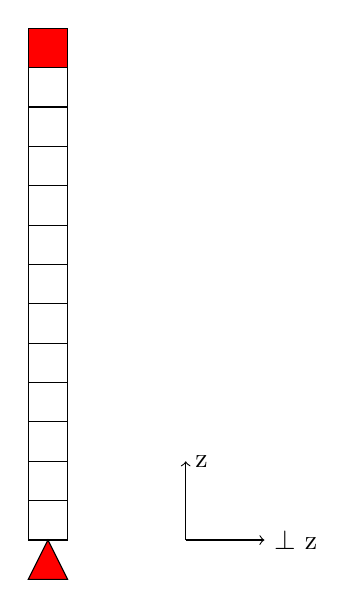
\begin{tikzpicture}
\foreach \x in {1,..., 12} \draw(0, 0.5*\x-0.5) rectangle +(.5,.5);
\filldraw[fill=red] (0, 6) rectangle +(.5,.5); 
\filldraw[fill=red] (0, -0.5) -- (0.25, 0) -- (0.5, -0.5) -- cycle;
\draw[->] (2,0) -- (2, 1) node[anchor=west] {z};
\draw[->] (2,0) -- (3, 0) node[anchor=west] {$\perp$ z};
\end{tikzpicture}
\caption{Geometry for test problems.}
\label{fig:exp_geometry}
\end{figure}

The two problems, while having the same geometry, are different in their dominant physics.
One problem was designed to simulate single-phase, single-field continuous liquid flow in a standpipe.
This problem will be referred to as the single-phase problem.
The second problem was designed such that high-pressure liquid flashes into steam as it enters a standpipe initially filled with saturated vapor at a much lower pressure, known hereafter as the flashing problem.

\tab{tab:ic} provides the initial conditions for the two problems.
The pressure, enthalpy, and volume-fractions for the different fields allow for a complete description of the continuity variables.
The initial velocities are set to zero.

\begin{table}[ht]
\centering
\singlespace
\pgfplotstabletypeset[fixed zerofill, col sep=comma,
	columns/problem/.style={column name=,string type, column type=l},
	columns/p/.style={ column name=Pressure,dec sep align, precision=1},
	columns/h/.style={ column name=Enthalpy,dec sep align, precision=1},
	columns/a_g/.style={ column name=$\alpha_g$, precision=1},
	columns/a_l/.style={ column name=$\alpha_l$, precision=1},
	columns/a_e/.style={ column name=$\alpha_e$, precision=1},
	every head row/.style={
		before row=\toprule,
		after row={& \multicolumn{2}{c}{$[\text{psia}]$} &\multicolumn{2}{c}{$[\frac{\text{BTU}}{\lbm{}}]$} &$[\text{-}]$ & $[\text{-}]$ & $[\text{-}]$\\ \midrule}},
	every last row/.style={
after row=\bottomrule}]{tables/data_ic_nln.tex}

\caption{Initial conditions for test problems.}
\label{tab:ic}
\end{table}

Each of the problems has a specified pressure-enthalpy boundary condition at the top of the stand pipe and a flow-enthalpy boundary condition at the inlet of the domain.
\tab{tab:bc_pe} contains the pressure, enthalpy, and composition of the pressure-enthalpy reservoir. 

\begin{table}[h!t]
\centering
\singlespace
\pgfplotstabletypeset[fixed zerofill, col sep=comma,
	columns/problem/.style={column name=,string type, column type=l},
	columns/p/.style={ column name=Pressure,dec sep align, precision=1},
	columns/h/.style={ column name=Enthalpy,dec sep align, precision=1},
	columns/a_g/.style={ column name=$\alpha_g$, precision=1},
	columns/a_l/.style={ column name=$\alpha_l$, precision=1},
	columns/a_e/.style={ column name=$\alpha_e$, precision=1},
	every head row/.style={
		before row=\toprule,
		after row={& \multicolumn{2}{c}{$[\text{psia}]$} &\multicolumn{2}{c}{$[\frac{\text{BTU}}{\lbm{}}]$} &$[\text{-}]$ & $[\text{-}]$ & $[\text{-}]$\\ \midrule}},
	every last row/.style={
after row=\bottomrule}]{tables/data_bc_outflow_nln.tex}

\caption{The pressure-enthalpy outlet boundary conditions for test problems.}
\label{tab:bc_pe}
\end{table}

The flow-enthalpy boundary condition describes the thermodynamic state of the in-flowing fluid and its flow rate.
\tab{tab:bc_fe} describes the inlet boundary condition for the two problems.

\begin{table}[ht]
\centering
\singlespace
\pgfplotstabletypeset[fixed zerofill, col sep=comma,
	columns/problem/.style={column name=,string type, column type=l},
	columns/p/.style={ column name=Pressure,dec sep align, precision=1},
	columns/h/.style={ column name=Enthalpy,dec sep align, precision=1},
	columns/a_g/.style={ column name=$\alpha_g$, precision=1},
	columns/a_l/.style={ column name=$\alpha_l$, precision=1},
	columns/a_e/.style={ column name=$\alpha_e$, precision=1},
	every head row/.style={
		before row=\toprule,
		after row={& \multicolumn{2}{c}{$[\text{psia}]$} &\multicolumn{2}{c}{$[\frac{\text{BTU}}{\lbm{}}]$} &$[\text{-}]$ & $[\text{-}]$ & $[\text{-}]$\\ \midrule}},
	every last row/.style={
after row=\bottomrule}]{tables/data_bc_inflow_nln.tex}

\caption{The flow-enthalpy inlet boundary conditions for test problems.}
\label{tab:bc_fe}
\end{table}

The specified mass flow, $\dot{m}(t)$, at the bottom of the channels is the same for both problems. 
This time-dependent function is given by \eqref{eqn:bc_time_func_single}.

\begin{equation}
\label{eqn:bc_time_func_single}
\dot{m}(t) = \left\{
\begin{array}{cclrcll}
 0.0           & [\frac{ \lbm{} }{\text{s}}] & , &                & t & \leq 1 & [\text{s}] \\
 0.5 ( t - 1)  & [\frac{ \lbm{} }{\text{s}}] & , & 1\; [\text{s}] < & t & \leq 2 & [\text{s}] \\
 0.5           & [\frac{ \lbm{} }{\text{s}}] & , &                & t & > 2    & [\text{s}]
\end{array}\right.
\end{equation}

Both problems adjust their initial pressure distribution to account for hydrostatic head.

\subsection{Results}
\label{subsect:single_results}

The results from the simulation runs will now be analyzed to determine the impact of nonlinear convergence upon time-step size sensitivity.
The solutions produced by both solvers will be compared to determine the efficacy of the residual metric in determining the validity of the nonlinear solution.  

For the flashing problem, the parameter of interest for temporal convergence testing is $\alpha_g$ at 2 [in] from the inlet of the stand pipe.
\fig{fig:flashing_1em1} shows the gaseous volume fraction 2 [in] from the inlet of the stand pipe as a function of time for a \dtmax{} of \expneg{1.0}{1} [s] for both the linear and the nonlinear solvers.

\begin{figure}[h!tb]
\centering
\includegraphics[width=0.6\textwidth]{plots/flashing_1em1.eps}
\caption{Flashing solution at \dtmax{} = \expneg{1.0}{1} {[s]}}
\label{fig:flashing_1em1}
\end{figure}

\begin{figure}[h!tb]
\centering
\includegraphics[width=.6\textwidth]{plots/flashing_1em5.eps}
\caption{Flashing solution at \dtmax{} = \expneg{1.0}{5} {[s]}.}
\label{fig:flashing_1em5}
\end{figure}

Note that the nonlinearly resolved solution is qualitatively different than the linear single-shot solution, \fig{fig:flashing_1em1}.
Even as the \dtmax{} is reduced, this discrepancy does not disappear, \fig{fig:flashing_1em5}.
The two solutions do not converge to the same solution as the timestep size was reduced.
However, the solution to the flashing problem produced by the nonlinear solver, \fig{fig:nl_mode_flashing}, qualitatively varies less as the timestep size is reduced than that produced by the linear solver, \fig{fig:cobra_mode_flashing}.
However, both \fig{fig:cobra_mode_flashing} and \fig{fig:nl_mode_flashing} show that as the timestep size is reduced the two different solutions become more timestep size insensitive.

\begin{figure}[h!tb]
\centering
\includegraphics[width=.6\textwidth]{plots/lin_flashing_al_2in.eps}
\caption{Linear solver flashing solution.}
\label{fig:cobra_mode_flashing}
\end{figure}

\begin{figure}[h!bt]
\centering
\includegraphics[width=.6\textwidth]{plots/nln_flashing_al_2in.eps}
\caption{Nonlinear solver flashing solution.}
\label{fig:nl_mode_flashing}
\end{figure}

The two solvers, when applied to the same problem that contains highly nonlinear physics, produce two different timestep size invariant solutions.
These two solutions achieve qualitative timestep size invariance at different timestep sizes.
The parameter of interest in the solution produced by the nonlinear solver with a 1 [s] \dtmax{} is qualitatively close to that produced with a 0.1 [s] \dtmax{}, \fig{fig:nl_flashing_compare}.
The same level of qualitative timestep size invariance is achieved in the linear solver solutions between a \dtmax{} of \expneg{1.0}{3} [s] and \expneg{1.0}{4} [s], \fig{fig:cobra_flashing_compare}.

\begin{figure}[h!bt]
\centering
\includegraphics[width=.6\textwidth]{plots/nln_flashing_1em0_1em1.eps}
\caption{Nonlinear solver timestep size insensitive flashing solution.}
\label{fig:nl_flashing_compare}
\end{figure}

\begin{figure}[h!tb]
\centering
\includegraphics[width=.6\textwidth]{plots/lin_flashing_1em1_1em4.eps}
\caption{Linear solver timestep size insensitive flashing solution.}
\label{fig:cobra_flashing_compare}
\end{figure}

The timestep size insensitive solution produced by the nonlinear solver occurs at a maximum timestep size three orders of magnitude greater than that achieved by the linear solver in \cobra{}.
An examination of the nonlinear residual over the course of the transient provides insight into why this behavior is observed.
The scaled residual for the linear flashing problem indicates that, even for small timestep sizes, the solution obtained still does not satisfy the discrete nonlinear equations, \fig{fig:linear_flashing_residual}.
This is in contrast to the nonlinear flashing problem, which shows a lower residual over the course of the simulation, \fig{fig:nonlinear_flashing_residual}.

\begin{figure}[h!tb]
\centering
\includegraphics[width=0.6\textwidth]{plots/lin_flashing_res_compare.eps}
\caption{Residual of the flashing solution for the linear solver.}
\label{fig:linear_flashing_residual}
\end{figure}

\begin{figure}[h!tb]
\centering
\includegraphics[width=0.6\textwidth]{plots/nln_flashing_res_compare.eps}
\caption{Residual of the flashing solution for the nonlinear solver.}
\label{fig:nonlinear_flashing_residual}
\end{figure}

The reduction in the residual exhibited by the solution produced by the linear solver, \fig{fig:linear_flashing_residual}, shows that the reduction of the maximum allowable timestep size now serves two purposes.
The first is that as \dtmax{} is reduced the nonlinear physics are being better resolved; however, even for small \dtmax{}, the residuals are still large compared to those of the nonlinear solution, \fig{fig:nonlinear_flashing_residual}.
The second purpose in reducing \dtmax{} is to decrease the error due to the discrete approximation of the temporal integral of the governing equations.
While the reduction of the maximum timestep size in the linear solver serves the purpose of reducing the residual, the nonlinear solver performs this task naturally.
Therefore, in the nonlinear solver the reduction of the maximum timestep size primarily serves to reduce the error from the approximate discrete temporal integral.

\begin{figure}[h!tb]
\centering
\includegraphics[width=0.6\textwidth]{plots/single_1em0.eps}
\caption{Single-phase solution with \dtmax{} = 1.0 {[s]}.}
\label{fig:single_1em1}
\end{figure}

\begin{figure}[h!tb]
\centering
\includegraphics[width=0.6\textwidth]{plots/single_1em5.eps}
\caption{Single-phase solution with \dtmax{} = \expneg{1.0}{5} {[s]}.}
\label{fig:single_1em5}
\end{figure}

The single-phase case was designed to test if the linear solver produced a simulation result that was equivalent to that produced by the nonlinear solver.
More specifically, it was designed to show that for problems where the physics of interest have relatively low nonlinearities, the linear solver provides as accurate a solution as the nonlinear solver.
\fig{fig:single_1em1} and \fig{fig:single_1em5} show the solution produced by both the nonlinear and linear solvers of \cobra{}.
Unlike the flashing problem, both solvers were able to solve the problem for all of the \dtmax{} specified.
The solutions produced by both solvers are qualitatively equivalent at \dtmax{} = 1.0 [s] and \dtmax{} = \expneg{1.0}{5} [s].
This indicates that the linear solver is adequate in regions where the solution is not highly nonlinear.

One way to quantify the difference between the solutions is by measuring the residual convergence metrics outlined in \sect{sect:temporal_convergence}.
These metrics provide a measure of how poorly the discrete nonlinear equations are being solved at every timestep in the transient.
The resolution of the residual allows for a solution that is less sensitive to timestep size selection than for a solution that does not resolve the residual.
The convergence metrics will be used to determine if a qualitative temporal-convergence determination can lead to the acceptance of a solution that is not nonlinearly converged.

For each of the test cases, the two different metrics were compared at the different \dtmax{}.
To examine efficacy of the the temporal convergence criteria, both the average and moment based temporal convergence criteria were evaluated for each of the twenty-three successful simulations.
The values of these metrics will be compared between different solvers for the same test problem. 

The two different nonlinear convergence metrics will now be examined for the flashing problem.
\tab{tab:flashing_criteria} shows both the average metric, $\tilde{R}$, and the moment based metric, $\tilde{R}_{\text{M}}$.

\begin{table}[h!t]
\centering
\singlespace
\pgfplotstabletypeset[sci zerofill,sci E, col sep=comma,
	columns/0/.style={ column name=\dtmax{}, precision=1},
	columns/1/.style={ column name=Linear, precision=3},
	columns/2/.style={ column name=Nonlinear, precision=3},
	columns/3/.style={ column name=Linear, precision=3},
	columns/4/.style={ column name=Nonlinear, precision=3},
	every head row/.style={
		before row={
			\toprule
			&\multicolumn{2}{c}{$\tilde{R}$} & \multicolumn{2}{c}{$\tilde{R}_{M}$}\\
		},
		after row=\midrule
	},
	every last row/.style={
after row=\bottomrule}]{tables/data_flashing_metric.tex}
\caption{Nonlinear convergence metrics for flashing problem.}
\label{tab:flashing_criteria}
\end{table}

\begin{table}[h!t]
\centering
\singlespace
\pgfplotstabletypeset[sci zerofill,sci E, col sep=comma,
	columns/0/.style={ column name=\dtmax{}, precision=1},
	columns/1/.style={ column name=Linear, precision=3},
	columns/2/.style={ column name=Nonlinear, precision=3},
	columns/3/.style={ column name=Linear, precision=3},
	columns/4/.style={ column name=Nonlinear, precision=3},
	every head row/.style={
		before row={
			\toprule
			&\multicolumn{2}{c}{$\tilde{R}$} & \multicolumn{2}{c}{$\tilde{R}_{M}$}\\
		},
		after row=\midrule
	},
	every last row/.style={
after row=\bottomrule}]{tables/data_single_metric.tex}
\caption{Nonlinear convergence metrics for the single-phase problem.}
\label{tab:single_criteria}
\end{table}

\tab{tab:single_criteria} shows the two metrics for the single-phase problem.

%============================================================================
% Problem that shows that the domain decomposition algorithm is implemented correctly.
%============================================================================
\section{Complex Geometry Problem}
\label{sect:complexProblem}
The complex geometry problem tests to determine if the domain decomposition algorithm is implemented properly.
To properly test the domain decomposition algorithm many different permutations of the composition of the nonlinear domain are required.
The presence of both axial momentum flow paths and transverse momentum flow paths is necessary.
If the nonlinear domain of the decomposed problem is subjected to just a single Newton step, then the resulting dual domain solution should match within numerical round off that of a single domain with a single Newton step regardless of the composition of the nonlinear domain.
A model of the General Electric nine-rod subchannel experimental facility \cite{Lahey1970} suites the requirements of this test.

\subsection{Model}
\label{sect:complexModel}

The General Electric experiments were conducted in an experimental facility with a nine-rod bundle representative of a BWR channel.
The basic layout of the portion of the facility that is of interest to this work is as follows.
There is an inlet plenum that is opens into a nine-rod bundles as depicted in \fig{fig:channel_layout}.
Above the rod-bundle there is an outlet plenum.

\begin{figure}[ht]
\centering
\begin{center}
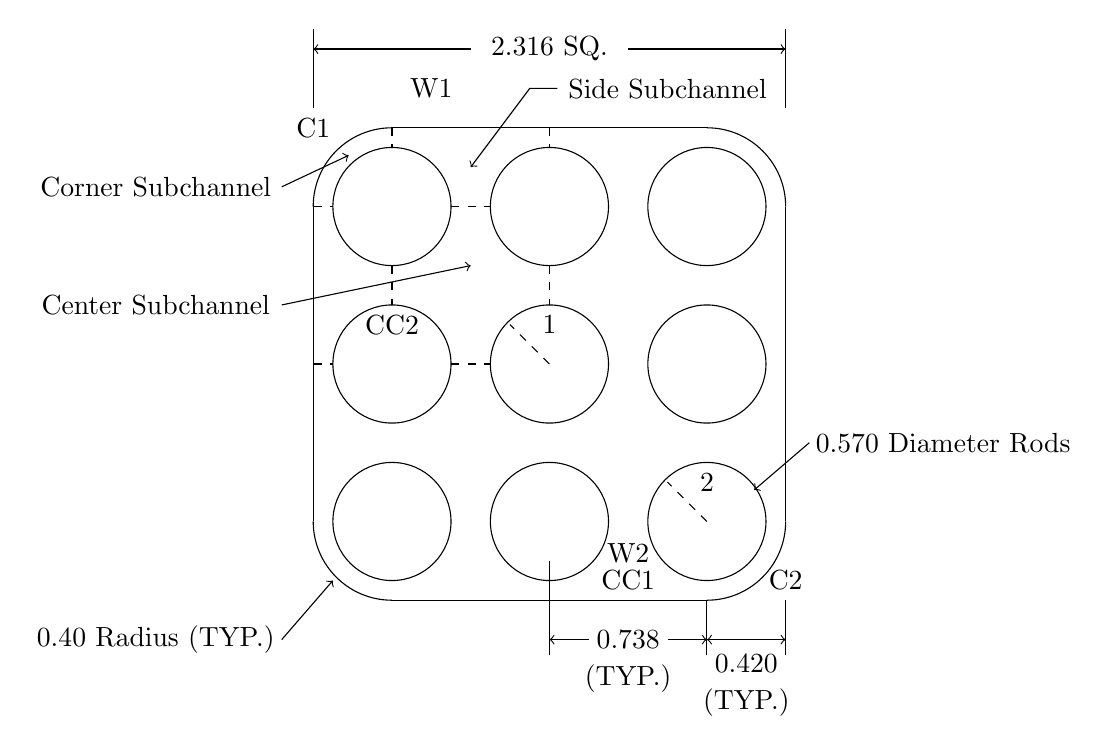
\begin{tikzpicture}

%Rounded corners
\draw (3,2) arc (0:90:1);
\draw (-2,3) arc (90:180:1);
\draw (-3,-2) arc (180:270:1);
\draw (2,-3) arc (270:360:1);

%Grid of circles
\draw (0,0) circle (0.75);
\draw (0,2) circle (0.75);
\draw (0,-2) circle (0.75);
\draw (2,0) circle (0.75);
\draw (2,2) circle (0.75);
\draw (2,-2) circle (0.75);
\draw (-2,0) circle (0.75);
\draw (-2,2) circle (0.75);
\draw (-2,-2) circle (0.75);

%Box
\draw (-3,-2) -- (-3,2);
\draw (3,-2) -- (3,2);
\draw (2,-3) -- (-2,-3);
\draw (-2,3) -- (2,3);

%Misc lines
\draw [dashed] (-2,3) -- (-2,2.75);
\draw [dashed] (0,3) -- (0,2.75);
\draw [dashed] (-2,1.25) -- (-2,0.75);
\draw [dashed] (0,1.25) -- (0,0.75);
\draw [dashed] (-3,2) -- (-2.75,2);
\draw [dashed] (-3,0) -- (-2.75,0);
\draw [dashed] (-1.25,2) -- (-0.75,2);
\draw [dashed] (-1.25,0) -- (-0.75,0);

\draw [dashed] (0,0) -- (-0.5,0.5);
\draw [dashed] (2,-2) -- (1.5,-1.5);

%Misc arrows and labels
\draw [<-] (-3,4) -- (-1,4);
\draw [->] (1,4) -- (3,4);
\draw (-3,4.25) -- (-3,3.25);
\draw (3,4.25) -- (3,3.25);
\draw (0,4) node {2.316 SQ.};

\draw [<-] (0,-3.5) -- (0.5,-3.5);
\draw [->] (1.5,-3.5) -- (2,-3.5);
\draw (2,-3.7) -- (2,-3);
\draw (0,-3.7) -- (0,-2.5);
\draw (1,-3.5) node {0.738};
\draw (1,-4) node {(TYP.)};

\draw [<->] (2,-3.5) -- (3,-3.5);
\draw (3,-3.7) -- (3,-3);
\draw (2.5,-3.8) node {0.420};
\draw (2.5,-4.3) node {(TYP.)};

\draw [->] (-3.4,2.25) -- (-2.55,2.65);
\draw (-5,2.25) node {Corner Subchannel};

\draw [->] (-3.4,0.75) -- (-1,1.25);
\draw (-5,0.75) node {Center Subchannel};

\draw [->] (0.1,3.5) -- (-0.25,3.5) -- (-1,2.5);
\draw (1.5,3.5) node {Side Subchannel};

\draw [->] (-3.4,-3.5) -- (-2.75,-2.75);
\draw (-5,-3.5) node {0.40 Radius (TYP.)};

\draw [->] (3.3,-1) -- (2.6,-1.6);
\draw (5,-1) node {0.570 Diameter Rods};

\draw (-3,3) node {C1};
\draw (-1.5,3.5) node {W1};
\draw (1,-2.75) node {CC1};

\draw (3,-2.75) node {C2};
\draw (1,-2.4) node {W2};
\draw (-2,0.5) node {CC2};

\draw (0,0.5) node {1};
\draw (2,-1.5) node {2};

\end{tikzpicture}
\end{center}
\caption{Position of pressure taps for setting isokinetic conditions. Note splitter positions for the various subchannels.}
\label{fig:position_of_pressure taps}
\caption{Position of Pressure Taps for Setting Isokinetic Conditions \cite{Lahey1970}.}
\label{fig:channel_layout}
\end{figure}

The \cobra{} model is broken into three sections.
The first section is the inlet plenum, while the third section is the outlet plenum.
The inlet plenum is 12 [in] tall with a cross-sectional area of 2.93 $[ \text{in}^2]$.
The outlet plenum is identically dimensioned.
The second section represents the rod-bundle.
This section is 121.5 [in] tall.
The rod-bundle is approximated by sixteen channels.
There are four corner subchannels, eight side subchannels, and four center subchannels in the model.
The dimensions for the various channels are shown in \fig{fig:channel_layout} is given.

There were a diverse collection of simulations run in this facility.
The run known as 2B-3 was chosen as the basis for this simulation.
Since the primary purpose of this problem is to test the ability of the domain decomposition algorithm to accurately recover the linear solution when the nonlinear domain is restricted to a single Newton step, the details of the boundary and initial conditions are omitted here.
The exact geometric details can be found in the technical report \cite{Lahey1970}.

There eighteen channels in this model.
That means that there are $2^{18}$ possible ways to decompose this problem with the domain decomposition algorithm.
The time required to run that many simulations is prohibitive, so only a subset are simulated here.
To test if the domain decomposition algorithm was implemented correctly, two-hundred and fifty-six different permutations were selected at random and run.
Of these 256, one was the purely linear case, and one was the purely nonlinear case.
The other 254 cases were generated by selecting a random number of random channel ids.

\subsection{Results}
\label{sect:complexResults}

First, it should be noted that the traditional output file of variables for \cobra{} is a single precision file.
This is important because the results obtained via this test were identical to single precision.
This required modifications of the software to generate additional double precision numbers to compare.

These results indicate that the domain decomposition algorithm was implemented as intended.

%============================================================================
% Problem that shows that when it is possible to isolate the nonlinearities, the computational cost can be lower.
%============================================================================
\section{Valve Type Problem}
\label{sect:valveProblem}
This problem is designed to demonstrate the ability of the domain decomposition algorithm to resolve isolated nonlinearities at a lower computational cost than the fully nonlinear solver. 
First, the model will be discussed and initial and boundary conditions provided.
Second, a timestep sensitivity study of the solution for both the linear and the nonlinear solver will be conducted.
Next, the portion of the domain with the nonlinearities will be isolated via the domain decomposition algorithm and another timestep sensitivity study will be conducted.
Finally, the solution and run time data from the three methods will be compared.

\subsection{Model}
\label{subsect:valveModel}

The physical system being modeled is that of four pipes.
Each pipe is 40 [in] tall, with a cross-sectional area, $ A_{c} $, of 16 $[\text{in}^{2}]$.
Two pipes have a fixed obstruction, manifesting as a loss coefficients, along their lengths.
One pipe has a complete obstruction, preventing flow.
The last pipe has a boundary condition that imitates the behavior of a valve by using a  time dependent loss coefficient at one point.
Initially fully open, the valve slowly closes.
While closing, the valve stops twice at cross-sectional areas that are equivalent to the two loss coefficients of the two partially obstructed pipes.
After fully closing, the valve returns to the first stopping point.

The pipe is initially full of subcooled liquid at 800 $[ \text{psia}] $.
The bottom and top of the pipe are open to reservoirs.
The bottom reservoir is full of subcooled liquid with a time variant pressure.
The pressure starts at at 802 $[ \text{psia} ] $ and increases to 818 $[ \text{psia}]$ over the first second, staying there for the duration of the problem.
The top reservoir is full of subcooled liquid at 800 $[\text{psia} ] $.
This pressure does not change as a function of time.
The $\Delta P$ that exists between these two reservoirs is what drives the flow in this problem.

The model used in \cobra{} is a single section.
Within that section there are four channels.
These channels are hydrodynamically isolated from each other.
They correspond to the four pipes.
The two partially-obstructed pipes have user-defined loss coefficients placed 15 [in] up the pipe.
The two coefficients are 40 $[-]$ and 160 $[-]$.
The fully-obstructed channel has a no-flow boundary condition at 15 [in].
The fourth channel has a time dependent area ratio multiplier, $A(t)_r$, at 15 [in].
This multiplier acts to reduce the area of the momentum flow path, $A_m$, used in the determination of form losses and wall drag.
However, these four channels have had their wall drag terms artificially reduced.
Reducing the wall drag allows the impact of the loss coefficients upon the solution to be isolated.
Since there is no wall drag in this problem, the area ratio is can be related to the effective loss coefficient by \eqref{eqn:valveLossCoefficient}.

\begin{equation}
\label{eqn:valveLossCoefficient}
K(t) = \frac{K_{o}}{{A(t)_r}^2}
\end{equation}

The base loss coefficient, $K_o$, for channel four is 10 [-].
Using \eqref{eqn:valveLossCoefficient}, the equivalent area ratios for the loss coefficients of the two partially obstructed pipes, 40 [-] and 160 [-], are 0.5 and 0.25 respectively.
The time dependent area ratio multiplier for channel four is given by \eqref{eqn:valveTransLoss}.

\begin{equation}
\label{eqn:valveTransLoss}
A(t)_{r} = \left\{
\begin{array}{cclrcll}
 1.0 & [-] & , & & t & \leq 3 & [\text{s}] \\
 1.0 - 0.5 \left( t - 3\right) & [-] & , & 3\; [\text{s}] < & t & \leq 4 & [\text{s}] \\
 0.5 & [-] & , & 4\; [\text{s}] < & t & \leq 7 & [\text{s}] \\
 0.5 - 0.25 \left( t - 7\right) & [-] & , &  7\; [\text{s}] < & t & \leq 8 & [\text{s}] \\
 0.25 & [-] & , & 8\; [\text{s}] < & t & \leq 11 & [\text{s}] \\
 0.25 - 0.25 \left( t - 11\right) & [-] & , & 11\; [\text{s}] < & t & \leq 12 & [\text{s}] \\
 0 & [-] & , & 12\; [\text{s}] < & t & \leq 15 & [\text{s}] \\
 0.5 \left( t - 15\right) & [-] & , & & t & > 16 & [\text{s}]
\end{array}\right.
\end{equation}

The simulation is run to an end time of 19 seconds.
The functional form of the transient area boundary condition was chosen so that the solution of the transient area pipe would mimic the three other pipes for portions of the transient.

\subsection{Results}
\label{subsect:valveResults}

The parameter of interest is the flow of liquid at the 15 [in] above the inlet.
This location corresponds to the location of the loss coefficients, the no-flow boundary condition, and the variable momentum-area boundary condition in the four pipes.
An automated procedure was used to conduct the timestep sensitivity study.
Given an initial \dtmax{}, $\dtmax{}_{o}$, a refinement factor, $r_{f}$, and the number of timestep size refinements to be taken, $n$, the simulation was run with both the linear solver and the nonlinear solver for each \dtmax{} in the set calculated according to \eqref{eqn:timeStepAlgo}.

\begin{equation}
\label{eqn:timeStepAlgo}
\dtmax{} \in \bigcup^{n-1}_{i\, = 0} \frac{\dtmax{}_{o}}{r^{i}_{f}}
\end{equation}

For this study, the three parameters, $\dtmax{}_{o}$, $r_{f}$, and $n$, were 1.0, 2.0, and 10, respectively.
Upon examining the solution, it was determined that timestep size was \dtcrnt{} limited for a portion of the transient until \dtmax{} = \expneg{1.56}{2}{[s]} was reached.
The timestep history of the simulations from \dtmax{} = 1.0 through \dtmax{} = \expneg{6.25}{2}{[s]} were identical for both the linear and the nonlinear solution.
The first four simulation results for each solver were dropped from the data sets since they represented duplicated results.
The solution obtained with \dtmax{} = \expneg{6.25}{2}{[s]} with the linear solver is shown in \fig{fig:valveLin6pt25em02}.

\begin{figure}[h!t]
\centering
% This file was created by matlab2tikz v0.4.3.
% Copyright (c) 2008--2013, Nico Schlömer <nico.schloemer@gmail.com>
% All rights reserved.
% 
\tikzsetnextfilename{plots/valveLin6pt2500em02_pdf}
\begin{tikzpicture}

\begin{axis}[%
width=\mytikzpicwidth,
height=\mytikzpicheight,
scale only axis,
xmin=0,
xmax=19,
xlabel={Time $[\text{s}]$},
ymin=-5,
ymax=125,
ylabel={Flow Rate $[ \frac{\lbm{}}{\text{s}} ]$},
legend style={draw=black,fill=white,legend cell align=left}
]
\addplot [
color=black,
solid
]
table[row sep=crcr]{
0 0\\
9.99999974737875e-06 7.3426820179634e-09\\
2.49999993684469e-05 6.82794052409008e-07\\
4.75000015285332e-05 1.61540210683597e-05\\
8.12500002211891e-05 0.000229488563491032\\
0.000131875000079162 0.00192578241694719\\
0.000207812496228144 0.00898927729576826\\
0.000321718747727573 0.023475144058466\\
0.000492578139528632 0.0383497066795826\\
0.00074886716902256 0.0502717047929764\\
0.00113330082967877 0.0704957619309425\\
0.00170995120424777 0.1085309907794\\
0.00257492670789361 0.167750924825668\\
0.00387239013798535 0.25895568728447\\
0.00529959984123707 0.363645792007446\\
0.00686953077092767 0.484240502119064\\
0.0085964547470212 0.623413980007172\\
0.0104960706084967 0.784365355968475\\
0.0125856483355165 0.970891773700714\\
0.014884184114635 1.18749308586121\\
0.0174125730991364 1.43950164318085\\
0.020193800330162 1.73323345184326\\
0.0232531521469355 2.07616090774536\\
0.0266184378415346 2.4771089553833\\
0.0303202513605356 2.94646978378296\\
0.0343922488391399 3.49643588066101\\
0.0388714447617531 4.14123106002808\\
0.0437985584139824 4.89732694625854\\
0.0492183864116669 5.78360366821289\\
0.0551801957190037 6.8213996887207\\
0.0617381855845451 8.03437232971191\\
0.0689519718289375 9.44805526733398\\
0.0768871381878853 11.0889587402344\\
0.0856158286333084 12.9830656051636\\
0.095217376947403 15.1535520553589\\
0.105779089033604 17.6176853179932\\
0.117396965622902 20.3830242156982\\
0.13017663359642 23.4434223175049\\
0.144234269857407 26.7757205963135\\
0.159697666764259 30.3384552001953\\
0.176707401871681 34.0738868713379\\
0.195418119430542 37.9140815734863\\
0.215999901294708 41.790412902832\\
0.238639861345291 45.644416809082\\
0.2635438144207 49.436939239502\\
0.290938168764114 53.1529197692871\\
0.321071952581406 56.8006935119629\\
0.354219108819962 60.406681060791\\
0.390680998563766 64.007698059082\\
0.427072286605835 67.3160705566406\\
0.461725652217865 70.2629699707031\\
0.494970262050629 72.9423904418945\\
0.527021527290344 75.4129028320313\\
0.55803918838501 77.7141189575195\\
0.588148653507233 79.8743591308594\\
0.617450594902039 81.914680480957\\
0.646027386188507 83.8512649536133\\
0.67394757270813 85.6969223022461\\
0.701269030570984 87.4619827270508\\
0.728040993213654 89.1549606323242\\
0.754306197166443 90.7829818725586\\
0.780101537704468 92.3520812988281\\
0.805459678173065 93.8674163818359\\
0.830409228801727 95.3334503173828\\
0.854975879192352 96.7540817260742\\
0.8791823387146 98.1327209472656\\
0.903049230575562 99.4723892211914\\
0.926595151424408 100.775764465332\\
0.949836909770966 102.04524230957\\
0.972789883613586 103.282974243164\\
0.995468020439148 104.49089050293\\
1.01788425445557 105.216697692871\\
1.0400505065918 105.585403442383\\
1.06216442584991 105.77458190918\\
1.08427441120148 105.871871948242\\
1.10638225078583 105.921897888184\\
1.12848901748657 105.947624206543\\
1.15059518814087 105.96085357666\\
1.1727010011673 105.967651367188\\
1.19480681419373 105.971153259277\\
1.21691238880157 105.972953796387\\
1.23901796340942 105.973876953125\\
1.26112222671509 105.974349975586\\
1.28322517871857 105.974594116211\\
1.30532777309418 105.974716186523\\
1.32742953300476 105.974784851074\\
1.34953081607819 105.974815368652\\
1.37163174152374 105.974830627441\\
1.39373195171356 105.974838256836\\
1.41583180427551 105.97484588623\\
1.43793165683746 105.97484588623\\
1.46003234386444 105.974853515625\\
1.48213422298431 105.974853515625\\
1.50423765182495 105.974853515625\\
1.52634274959564 105.974853515625\\
1.5484482049942 105.974853515625\\
1.57055377960205 105.974853515625\\
1.5926593542099 105.974853515625\\
1.61476469039917 105.974853515625\\
1.63686990737915 105.974853515625\\
1.65897512435913 105.974853515625\\
1.68108010292053 105.974853515625\\
1.70318508148193 105.974853515625\\
1.72528982162476 105.974853515625\\
1.74739444255829 105.974853515625\\
1.76949906349182 105.974853515625\\
1.79160356521606 105.974853515625\\
1.81370830535889 105.974853515625\\
1.83581340312958 105.974853515625\\
1.85791862010956 105.974853515625\\
1.88002419471741 105.974853515625\\
1.90212976932526 105.974853515625\\
1.92423534393311 105.974853515625\\
1.94634091854095 105.974853515625\\
1.9684464931488 105.974853515625\\
1.99055194854736 105.974853515625\\
2.01265740394592 105.974853515625\\
2.03476285934448 105.974853515625\\
2.05686831474304 105.974853515625\\
2.0789737701416 105.974853515625\\
2.10107922554016 105.974853515625\\
2.12318468093872 105.974853515625\\
2.14529013633728 105.974853515625\\
2.16739559173584 105.974853515625\\
2.1895010471344 105.974853515625\\
2.21160674095154 105.974853515625\\
2.2337121963501 105.974853515625\\
2.25581765174866 105.974853515625\\
2.2779233455658 105.974853515625\\
2.30002880096436 105.974853515625\\
2.32213449478149 105.974853515625\\
2.34423995018005 105.974853515625\\
2.36634540557861 105.974853515625\\
2.38845109939575 105.974853515625\\
2.41055655479431 105.974853515625\\
2.43266201019287 105.974853515625\\
2.45476770401001 105.974853515625\\
2.47687315940857 105.974853515625\\
2.49897861480713 105.974853515625\\
2.52108430862427 105.974853515625\\
2.54318976402283 105.974853515625\\
2.56529545783997 105.974853515625\\
2.58740091323853 105.974853515625\\
2.60950636863709 105.974853515625\\
2.63161206245422 105.974853515625\\
2.65371751785278 105.974853515625\\
2.67582321166992 105.974853515625\\
2.69792866706848 105.974853515625\\
2.72003412246704 105.974853515625\\
2.74213981628418 105.974853515625\\
2.76424527168274 105.974853515625\\
2.78635096549988 105.974853515625\\
2.80845642089844 105.974853515625\\
2.830561876297 105.974853515625\\
2.85266757011414 105.974853515625\\
2.8747730255127 105.974853515625\\
2.89687871932983 105.974853515625\\
2.91898417472839 105.974853515625\\
2.94108963012695 105.974853515625\\
2.96319532394409 105.974853515625\\
2.98530077934265 105.974853515625\\
3.00740647315979 105.783866882324\\
3.02951192855835 105.111946105957\\
3.05169749259949 104.186538696289\\
3.07412838935852 103.119384765625\\
3.09681701660156 101.971786499023\\
3.11977505683899 100.775596618652\\
3.14301300048828 99.5470809936523\\
3.16654181480408 98.2943115234375\\
3.19037246704102 97.0210647583008\\
3.21451687812805 95.7289123535156\\
3.23898792266846 94.4182662963867\\
3.26379895210266 93.0889282226563\\
3.28896427154541 91.7403869628906\\
3.31449961662292 90.371940612793\\
3.34042167663574 88.9827423095703\\
3.36674857139587 87.5718612670898\\
3.39349937438965 86.1382827758789\\
3.42069554328918 84.6808700561523\\
3.4483597278595 83.1984176635742\\
3.47651672363281 81.6895980834961\\
3.50519371032715 80.1529693603516\\
3.53442049026489 78.5869369506836\\
3.56422996520996 76.9897613525391\\
3.59465765953064 75.3595352172852\\
3.6257438659668 73.6941299438477\\
3.65753245353699 71.9911880493164\\
3.69007301330566 70.2481002807617\\
3.72342085838318 68.4618988037109\\
3.75763893127441 66.629280090332\\
3.79279804229736 64.746467590332\\
3.82897973060608 62.8091583251953\\
3.86627721786499 60.8124084472656\\
3.90479946136475 58.7504920959473\\
3.94467377662659 56.61669921875\\
3.9860508441925 54.4031181335449\\
4.02911138534546 53.2985801696777\\
4.07284307479858 53.053783416748\\
4.11683511734009 53.001636505127\\
4.16100072860718 52.9906539916992\\
4.20520448684692 52.9883499145508\\
4.24941444396973 52.987865447998\\
4.29362487792969 52.9877662658691\\
4.33783578872681 52.9877433776855\\
4.38204622268677 52.9877395629883\\
4.42625665664673 52.9877395629883\\
4.47046709060669 52.9877395629883\\
4.51467752456665 52.9877395629883\\
4.55888795852661 52.9877395629883\\
4.60309839248657 52.9877395629883\\
4.64730882644653 52.9877395629883\\
4.69151973724365 52.9877395629883\\
4.73573064804077 52.9877395629883\\
4.77994155883789 52.9877395629883\\
4.82415246963501 52.9877395629883\\
4.86836338043213 52.9877395629883\\
4.91257381439209 52.9877395629883\\
4.95678472518921 52.9877395629883\\
5.00099563598633 52.9877395629883\\
5.04520654678345 52.9877395629883\\
5.08941698074341 52.9877395629883\\
5.13362789154053 52.9877395629883\\
5.17783832550049 52.9877395629883\\
5.22204923629761 52.9877395629883\\
5.26626014709473 52.9877395629883\\
5.31047105789185 52.9877395629883\\
5.35468196868896 52.9877395629883\\
5.39889240264893 52.9877395629883\\
5.44310331344604 52.9877395629883\\
5.48731422424316 52.9877395629883\\
5.53152513504028 52.9877395629883\\
5.5757360458374 52.9877395629883\\
5.61994695663452 52.9877395629883\\
5.66415786743164 52.9877395629883\\
5.7083683013916 52.9877395629883\\
5.75257921218872 52.9877395629883\\
5.79679012298584 52.9877395629883\\
5.84100103378296 52.9877395629883\\
5.88521194458008 52.9877395629883\\
5.9294228553772 52.9877395629883\\
5.97363376617432 52.9877395629883\\
6.01784420013428 52.9877395629883\\
6.0620551109314 52.9877395629883\\
6.10626602172852 52.9877395629883\\
6.15047693252563 52.9877395629883\\
6.19468784332275 52.9877395629883\\
6.23889875411987 52.9877395629883\\
6.28310966491699 52.9877395629883\\
6.32732009887695 52.9877395629883\\
6.37153100967407 52.9877395629883\\
6.41574192047119 52.9877395629883\\
6.45995283126831 52.9877395629883\\
6.50416374206543 52.9877395629883\\
6.54837465286255 52.9877395629883\\
6.59258508682251 52.9877395629883\\
6.63679599761963 52.9877395629883\\
6.68100690841675 52.9877395629883\\
6.72521781921387 52.9877395629883\\
6.76942873001099 52.9877395629883\\
6.81363964080811 52.9877395629883\\
6.85785055160522 52.9877395629883\\
6.90206098556519 52.9877395629883\\
6.9462718963623 52.9877395629883\\
6.99048280715942 52.9877395629883\\
7.03469371795654 52.2620544433594\\
7.07890462875366 51.1824531555176\\
7.12311553955078 50.0258483886719\\
7.1673264503479 48.8525352478027\\
7.21153688430786 47.6756553649902\\
7.25574779510498 46.4980316162109\\
7.2999587059021 45.3202667236328\\
7.34416961669922 44.1424942016602\\
7.38838052749634 42.9647331237793\\
7.43259143829346 41.7869987487793\\
7.47680234909058 40.6092872619629\\
7.52101278305054 39.4316062927246\\
7.56522369384766 38.2539520263672\\
7.60943460464478 37.0763359069824\\
7.65364551544189 35.898754119873\\
7.69785642623901 34.7212142944336\\
7.74206733703613 33.5437202453613\\
7.78627824783325 32.3662757873535\\
7.83048868179321 31.1888885498047\\
7.87469959259033 30.0115623474121\\
7.91891050338745 28.8343067169189\\
7.96312141418457 27.6571311950684\\
8.00733184814453 26.6465225219727\\
8.05154323577881 26.5120487213135\\
8.09575366973877 26.4960327148438\\
8.13996505737305 26.4941577911377\\
8.18417549133301 26.4939384460449\\
8.22838687896729 26.4939117431641\\
8.27259731292725 26.4939098358154\\
8.31680774688721 26.4939098358154\\
8.36101913452148 26.4939079284668\\
8.40522956848145 26.4939079284668\\
8.44944095611572 26.4939079284668\\
8.49365139007568 26.4939079284668\\
8.53786277770996 26.4939079284668\\
8.58207321166992 26.4939079284668\\
8.62628364562988 26.4939079284668\\
8.67049503326416 26.4939079284668\\
8.71470546722412 26.4939079284668\\
8.7589168548584 26.4939079284668\\
8.80312728881836 26.4939079284668\\
8.84733867645264 26.4939079284668\\
8.8915491104126 26.4939079284668\\
8.93575954437256 26.4939079284668\\
8.97997093200684 26.4939079284668\\
9.0241813659668 26.4939079284668\\
9.06839275360107 26.4939079284668\\
9.11260318756104 26.4939079284668\\
9.156813621521 26.4939079284668\\
9.20102500915527 26.4939079284668\\
9.24523544311523 26.4939079284668\\
9.28944683074951 26.4939079284668\\
9.33365726470947 26.4939079284668\\
9.37786865234375 26.4939079284668\\
9.42207908630371 26.4939079284668\\
9.46628952026367 26.4939079284668\\
9.51050090789795 26.4939079284668\\
9.55471134185791 26.4939079284668\\
9.59892272949219 26.4939079284668\\
9.64313316345215 26.4939079284668\\
9.68734455108643 26.4939079284668\\
9.73155498504639 26.4939079284668\\
9.77576541900635 26.4939079284668\\
9.81997680664063 26.4939079284668\\
9.86418724060059 26.4939079284668\\
9.90839862823486 26.4939079284668\\
9.95260906219482 26.4939079284668\\
9.9968204498291 26.4939079284668\\
10.0410308837891 26.4939079284668\\
10.085241317749 26.4939079284668\\
10.1294527053833 26.4939079284668\\
10.1736631393433 26.4939079284668\\
10.2178745269775 26.4939079284668\\
10.2620849609375 26.4939079284668\\
10.3062963485718 26.4939079284668\\
10.3505067825317 26.4939079284668\\
10.3947172164917 26.4939079284668\\
10.438928604126 26.4939079284668\\
10.4831390380859 26.4939079284668\\
10.5273504257202 26.4939079284668\\
10.5715608596802 26.4939079284668\\
10.6157722473145 26.4939079284668\\
10.6599826812744 26.4939079284668\\
10.7041931152344 26.4939079284668\\
10.7484045028687 26.4939079284668\\
10.7926149368286 26.4939079284668\\
10.8368263244629 26.4939079284668\\
10.8810367584229 26.4939079284668\\
10.9252481460571 26.4939079284668\\
10.9694585800171 26.4939079284668\\
11.0136690139771 26.1752624511719\\
11.0578804016113 25.1147441864014\\
11.1020908355713 23.9547080993652\\
11.1463022232056 22.7804050445557\\
11.1905126571655 21.6041946411133\\
11.2347240447998 20.4278793334961\\
11.2789344787598 19.2517433166504\\
11.3231449127197 18.0758666992188\\
11.367356300354 16.9003086090088\\
11.411566734314 15.7251396179199\\
11.4557781219482 14.5504512786865\\
11.4778890609741 13.9317502975464\\
11.5 13.3384485244751\\
11.5243225097656 12.6927003860474\\
11.5510768890381 11.9840898513794\\
11.5805063247681 11.2058210372925\\
11.6128797531128 10.3513040542603\\
11.6484899520874 9.41370677947998\\
11.6876602172852 8.38610649108887\\
11.730749130249 7.26203107833862\\
11.774959564209 6.10678195953369\\
11.8191709518433 4.95429944992065\\
11.8633813858032 3.81441807746887\\
11.9075918197632 2.70163488388062\\
11.9518032073975 1.65573978424072\\
11.9960136413574 0.831265449523926\\
12.0402250289917 0\\
12.0844354629517 0\\
12.1286468505859 0\\
12.1728572845459 0\\
12.2170677185059 0\\
12.2612791061401 0\\
12.3054895401001 0\\
12.3497009277344 0\\
12.3939113616943 0\\
12.4381227493286 0\\
12.4823331832886 0\\
12.5265436172485 0\\
12.5707550048828 0\\
12.6149654388428 0\\
12.6591768264771 0\\
12.703387260437 0\\
12.7475986480713 0\\
12.7918090820313 0\\
12.8360195159912 0\\
12.8802309036255 0\\
12.9244413375854 0\\
12.9686527252197 0\\
13.0128631591797 0\\
13.057074546814 0\\
13.1012849807739 0\\
13.1454954147339 0\\
13.1897068023682 0\\
13.2339172363281 0\\
13.2781286239624 0\\
13.3223390579224 0\\
13.3665504455566 0\\
13.4107608795166 0\\
13.4549713134766 0\\
13.4991827011108 0\\
13.5433931350708 0\\
13.5876045227051 0\\
13.631814956665 0\\
13.6760263442993 0\\
13.7202367782593 0\\
13.7644472122192 0\\
13.8086585998535 0\\
13.8528690338135 0\\
13.8970804214478 0\\
13.9412908554077 0\\
13.985502243042 0\\
14.029712677002 0\\
14.0739231109619 0\\
14.1181344985962 0\\
14.1623449325562 0\\
14.2065563201904 0\\
14.2507667541504 0\\
14.2949781417847 0\\
14.3391885757446 0\\
14.3833990097046 0\\
14.4276103973389 0\\
14.4718208312988 0\\
14.5160322189331 0\\
14.5602426528931 0\\
14.6044540405273 0\\
14.6486644744873 0\\
14.6928749084473 0\\
14.7370862960815 0\\
14.7812967300415 0\\
14.8255081176758 0\\
14.8697185516357 0\\
14.9139289855957 0\\
14.95814037323 0\\
15.0023508071899 0.117176152765751\\
15.0465621948242 20.6927852630615\\
15.0907726287842 10.9598197937012\\
15.1349840164185 7.8855185508728\\
15.1791944503784 9.56354999542236\\
15.2234048843384 11.9345808029175\\
15.2676162719727 14.2009210586548\\
15.3118267059326 16.4927539825439\\
15.3560380935669 18.7888126373291\\
15.4002485275269 21.0889701843262\\
15.4444599151611 23.392017364502\\
15.4886703491211 25.6972122192383\\
15.5328807830811 28.0040435791016\\
15.5770921707153 30.3121509552002\\
15.6213026046753 32.621265411377\\
15.6655139923096 34.9311981201172\\
15.7097244262695 37.2417945861816\\
15.7539358139038 39.5529441833496\\
15.7981462478638 41.8645553588867\\
15.8423566818237 44.1765518188477\\
15.886568069458 46.488883972168\\
15.930778503418 48.8014984130859\\
15.9749898910522 51.1143608093262\\
16.0192012786865 52.6112480163574\\
16.0630474090576 52.9090232849121\\
16.1063537597656 52.9710159301758\\
16.1503849029541 52.9842262268066\\
16.1945571899414 52.987003326416\\
16.2387599945068 52.9875831604004\\
16.2829685211182 52.9877052307129\\
16.3271789550781 52.9877319335938\\
16.3713893890381 52.987735748291\\
16.4156017303467 52.9877395629883\\
16.4598121643066 52.9877395629883\\
16.5040225982666 52.9877395629883\\
16.5482330322266 52.9877395629883\\
16.5924434661865 52.9877395629883\\
16.6366558074951 52.9877395629883\\
16.6808662414551 52.9877395629883\\
16.725076675415 52.9877395629883\\
16.769287109375 52.9877395629883\\
16.813497543335 52.9877395629883\\
16.8577079772949 52.9877395629883\\
16.9019184112549 52.9877395629883\\
16.9461288452148 52.9877395629883\\
16.9903411865234 52.9877395629883\\
17.0345516204834 52.9877395629883\\
17.0787620544434 52.9877395629883\\
17.1229724884033 52.9877395629883\\
17.1671829223633 52.9877395629883\\
17.2113952636719 52.9877395629883\\
17.2556056976318 52.9877395629883\\
17.2998161315918 52.9877395629883\\
17.3440265655518 52.9877395629883\\
17.3882369995117 52.9877395629883\\
17.4324493408203 52.9877395629883\\
17.4766597747803 52.9877395629883\\
17.5208702087402 52.9877395629883\\
17.5650806427002 52.9877395629883\\
17.6092929840088 52.9877395629883\\
17.6535034179688 52.9877395629883\\
17.6977138519287 52.9877395629883\\
17.7419242858887 52.9877395629883\\
17.7861347198486 52.9877395629883\\
17.8303470611572 52.9877395629883\\
17.8745574951172 52.9877395629883\\
17.9187679290771 52.9877395629883\\
17.9629783630371 52.9877395629883\\
18.0071887969971 52.9877395629883\\
18.0514011383057 52.9877395629883\\
18.0956115722656 52.9877395629883\\
18.1398220062256 52.9877395629883\\
18.1840324401855 52.9877395629883\\
18.2282447814941 52.9877395629883\\
18.2724552154541 52.9877395629883\\
18.3166656494141 52.9877395629883\\
18.360876083374 52.9877395629883\\
18.405086517334 52.9877395629883\\
18.4492988586426 52.9877395629883\\
18.4935092926025 52.9877395629883\\
18.5377197265625 52.9877395629883\\
18.5819301605225 52.9877395629883\\
18.6261405944824 52.9877395629883\\
18.670352935791 52.9877395629883\\
18.714563369751 52.9877395629883\\
18.7587738037109 52.9877395629883\\
18.8029842376709 52.9877395629883\\
18.8471965789795 52.9877395629883\\
18.8914070129395 52.9877395629883\\
18.9356174468994 52.9877395629883\\
18.9678077697754 52.9877395629883\\
19 52.9877395629883\\
};
\addlegendentry{$A_{r}(t)$};

\addplot [
color=black,
dash pattern=on 1pt off 3pt on 3pt off 3pt
]
table[row sep=crcr]{
0 0\\
9.99999974737875e-06 7.34263050361506e-09\\
2.49999993684469e-05 6.82787117511907e-07\\
4.75000015285332e-05 1.61537918756949e-05\\
8.12500002211891e-05 0.000229484256124124\\
0.000131875000079162 0.00192573899403214\\
0.000207812496228144 0.00898905657231808\\
0.000321718747727573 0.0234745796769857\\
0.000492578139528632 0.0383488200604916\\
0.00074886716902256 0.0502703413367271\\
0.00113330082967877 0.0704929903149605\\
0.00170995120424777 0.108524538576603\\
0.00257492670789361 0.167731299996376\\
0.00387239013798535 0.258889704942703\\
0.00529959984123707 0.363474696874619\\
0.00686953077092767 0.483860403299332\\
0.0085964547470212 0.622648656368256\\
0.0104960706084967 0.782925307750702\\
0.0125856483355165 0.968311131000519\\
0.014884184114635 1.18303418159485\\
0.0174125730991364 1.43201053142548\\
0.020193800330162 1.72092187404633\\
0.0232531521469355 2.05627965927124\\
0.0266184378415346 2.44546175003052\\
0.0303202513605356 2.8966953754425\\
0.0343922488391399 3.41895937919617\\
0.0388714447617531 4.0217547416687\\
0.0437985584139824 4.71469640731812\\
0.0492183864116669 5.50687074661255\\
0.0551801957190037 6.40590953826904\\
0.0617381855845451 7.41679286956787\\
0.0689519718289375 8.54045581817627\\
0.0768871381878853 9.77241897583008\\
0.0856158286333084 11.1017980575562\\
0.095217376947403 12.5111665725708\\
0.105779089033604 13.9776849746704\\
0.117396965622902 15.4756441116333\\
0.13017663359642 16.9800872802734\\
0.144234269857407 18.4706878662109\\
0.159697666764259 19.9348068237305\\
0.176707401871681 21.3688697814941\\
0.195418119430542 22.7777843475342\\
0.215999901294708 24.1727924346924\\
0.238639861345291 25.5685958862305\\
0.2635438144207 26.9806213378906\\
0.290938168764114 28.4230575561523\\
0.321071952581406 29.907886505127\\
0.354219108819962 31.4447612762451\\
0.390680998563766 33.0414009094238\\
0.427072286605835 34.5504035949707\\
0.461725652217865 35.9212799072266\\
0.494970262050629 37.185417175293\\
0.527021527290344 38.3625907897949\\
0.55803918838501 39.4668655395508\\
0.588148653507233 40.5088539123535\\
0.617450594902039 41.4968566894531\\
0.646027386188507 42.4374961853027\\
0.67394757270813 43.3361740112305\\
0.701269030570984 44.1973571777344\\
0.728040993213654 45.024787902832\\
0.754306197166443 45.8216438293457\\
0.780101537704468 46.5906410217285\\
0.805459678173065 47.3341293334961\\
0.830409228801727 48.0541496276855\\
0.854975879192352 48.752498626709\\
0.8791823387146 49.4307518005371\\
0.903049230575562 50.0903167724609\\
0.926595151424408 50.7324409484863\\
0.949836909770966 51.3582496643066\\
0.972789883613586 51.9687538146973\\
0.995468020439148 52.5648574829102\\
1.01788425445557 52.8429985046387\\
1.0400505065918 52.9377365112305\\
1.06216442584991 52.9704132080078\\
1.08427441120148 52.9817276000977\\
1.10638225078583 52.9856491088867\\
1.12848901748657 52.9870109558105\\
1.15059518814087 52.9874839782715\\
1.1727010011673 52.9876518249512\\
1.19480681419373 52.9877090454102\\
1.21691238880157 52.9877319335938\\
1.23901796340942 52.9877395629883\\
1.26112222671509 52.9877395629883\\
1.28322517871857 52.9877433776855\\
1.30532777309418 52.9877433776855\\
1.32742953300476 52.9877395629883\\
1.34953081607819 52.9877395629883\\
1.37163174152374 52.9877395629883\\
1.39373195171356 52.9877395629883\\
1.41583180427551 52.9877395629883\\
1.43793165683746 52.9877395629883\\
1.46003234386444 52.9877395629883\\
1.48213422298431 52.9877395629883\\
1.50423765182495 52.9877395629883\\
1.52634274959564 52.9877395629883\\
1.5484482049942 52.9877395629883\\
1.57055377960205 52.9877395629883\\
1.5926593542099 52.9877395629883\\
1.61476469039917 52.9877395629883\\
1.63686990737915 52.9877395629883\\
1.65897512435913 52.9877395629883\\
1.68108010292053 52.9877395629883\\
1.70318508148193 52.9877395629883\\
1.72528982162476 52.9877395629883\\
1.74739444255829 52.9877395629883\\
1.76949906349182 52.9877395629883\\
1.79160356521606 52.9877395629883\\
1.81370830535889 52.9877395629883\\
1.83581340312958 52.9877395629883\\
1.85791862010956 52.9877395629883\\
1.88002419471741 52.9877395629883\\
1.90212976932526 52.9877395629883\\
1.92423534393311 52.9877395629883\\
1.94634091854095 52.9877395629883\\
1.9684464931488 52.9877395629883\\
1.99055194854736 52.9877395629883\\
2.01265740394592 52.9877395629883\\
2.03476285934448 52.9877395629883\\
2.05686831474304 52.9877395629883\\
2.0789737701416 52.9877395629883\\
2.10107922554016 52.9877395629883\\
2.12318468093872 52.9877395629883\\
2.14529013633728 52.9877395629883\\
2.16739559173584 52.9877395629883\\
2.1895010471344 52.9877395629883\\
2.21160674095154 52.9877395629883\\
2.2337121963501 52.9877395629883\\
2.25581765174866 52.9877395629883\\
2.2779233455658 52.9877395629883\\
2.30002880096436 52.9877395629883\\
2.32213449478149 52.9877395629883\\
2.34423995018005 52.9877395629883\\
2.36634540557861 52.9877395629883\\
2.38845109939575 52.9877395629883\\
2.41055655479431 52.9877395629883\\
2.43266201019287 52.9877395629883\\
2.45476770401001 52.9877395629883\\
2.47687315940857 52.9877395629883\\
2.49897861480713 52.9877395629883\\
2.52108430862427 52.9877395629883\\
2.54318976402283 52.9877395629883\\
2.56529545783997 52.9877395629883\\
2.58740091323853 52.9877395629883\\
2.60950636863709 52.9877395629883\\
2.63161206245422 52.9877395629883\\
2.65371751785278 52.9877395629883\\
2.67582321166992 52.9877395629883\\
2.69792866706848 52.9877395629883\\
2.72003412246704 52.9877395629883\\
2.74213981628418 52.9877395629883\\
2.76424527168274 52.9877395629883\\
2.78635096549988 52.9877395629883\\
2.80845642089844 52.9877395629883\\
2.830561876297 52.9877395629883\\
2.85266757011414 52.9877395629883\\
2.8747730255127 52.9877395629883\\
2.89687871932983 52.9877395629883\\
2.91898417472839 52.9877395629883\\
2.94108963012695 52.9877395629883\\
2.96319532394409 52.9877395629883\\
2.98530077934265 52.9877395629883\\
3.00740647315979 52.9877395629883\\
3.02951192855835 52.9877395629883\\
3.05169749259949 52.9877395629883\\
3.07412838935852 52.9877395629883\\
3.09681701660156 52.9877395629883\\
3.11977505683899 52.9877395629883\\
3.14301300048828 52.9877395629883\\
3.16654181480408 52.9877395629883\\
3.19037246704102 52.9877395629883\\
3.21451687812805 52.9877395629883\\
3.23898792266846 52.9877395629883\\
3.26379895210266 52.9877395629883\\
3.28896427154541 52.9877395629883\\
3.31449961662292 52.9877395629883\\
3.34042167663574 52.9877395629883\\
3.36674857139587 52.9877395629883\\
3.39349937438965 52.9877395629883\\
3.42069554328918 52.9877395629883\\
3.4483597278595 52.9877395629883\\
3.47651672363281 52.9877395629883\\
3.50519371032715 52.9877395629883\\
3.53442049026489 52.9877395629883\\
3.56422996520996 52.9877395629883\\
3.59465765953064 52.9877395629883\\
3.6257438659668 52.9877395629883\\
3.65753245353699 52.9877395629883\\
3.69007301330566 52.9877395629883\\
3.72342085838318 52.9877395629883\\
3.75763893127441 52.9877395629883\\
3.79279804229736 52.9877395629883\\
3.82897973060608 52.9877395629883\\
3.86627721786499 52.9877395629883\\
3.90479946136475 52.9877395629883\\
3.94467377662659 52.9877395629883\\
3.9860508441925 52.9877395629883\\
4.02911138534546 52.9877395629883\\
4.07284307479858 52.9877395629883\\
4.11683511734009 52.9877395629883\\
4.16100072860718 52.9877395629883\\
4.20520448684692 52.9877395629883\\
4.24941444396973 52.9877395629883\\
4.29362487792969 52.9877395629883\\
4.33783578872681 52.9877395629883\\
4.38204622268677 52.9877395629883\\
4.42625665664673 52.9877395629883\\
4.47046709060669 52.9877395629883\\
4.51467752456665 52.9877395629883\\
4.55888795852661 52.9877395629883\\
4.60309839248657 52.9877395629883\\
4.64730882644653 52.9877395629883\\
4.69151973724365 52.9877395629883\\
4.73573064804077 52.9877395629883\\
4.77994155883789 52.9877395629883\\
4.82415246963501 52.9877395629883\\
4.86836338043213 52.9877395629883\\
4.91257381439209 52.9877395629883\\
4.95678472518921 52.9877395629883\\
5.00099563598633 52.9877395629883\\
5.04520654678345 52.9877395629883\\
5.08941698074341 52.9877395629883\\
5.13362789154053 52.9877395629883\\
5.17783832550049 52.9877395629883\\
5.22204923629761 52.9877395629883\\
5.26626014709473 52.9877395629883\\
5.31047105789185 52.9877395629883\\
5.35468196868896 52.9877395629883\\
5.39889240264893 52.9877395629883\\
5.44310331344604 52.9877395629883\\
5.48731422424316 52.9877395629883\\
5.53152513504028 52.9877395629883\\
5.5757360458374 52.9877395629883\\
5.61994695663452 52.9877395629883\\
5.66415786743164 52.9877395629883\\
5.7083683013916 52.9877395629883\\
5.75257921218872 52.9877395629883\\
5.79679012298584 52.9877395629883\\
5.84100103378296 52.9877395629883\\
5.88521194458008 52.9877395629883\\
5.9294228553772 52.9877395629883\\
5.97363376617432 52.9877395629883\\
6.01784420013428 52.9877395629883\\
6.0620551109314 52.9877395629883\\
6.10626602172852 52.9877395629883\\
6.15047693252563 52.9877395629883\\
6.19468784332275 52.9877395629883\\
6.23889875411987 52.9877395629883\\
6.28310966491699 52.9877395629883\\
6.32732009887695 52.9877395629883\\
6.37153100967407 52.9877395629883\\
6.41574192047119 52.9877395629883\\
6.45995283126831 52.9877395629883\\
6.50416374206543 52.9877395629883\\
6.54837465286255 52.9877395629883\\
6.59258508682251 52.9877395629883\\
6.63679599761963 52.9877395629883\\
6.68100690841675 52.9877395629883\\
6.72521781921387 52.9877395629883\\
6.76942873001099 52.9877395629883\\
6.81363964080811 52.9877395629883\\
6.85785055160522 52.9877395629883\\
6.90206098556519 52.9877395629883\\
6.9462718963623 52.9877395629883\\
6.99048280715942 52.9877395629883\\
7.03469371795654 52.9877395629883\\
7.07890462875366 52.9877395629883\\
7.12311553955078 52.9877395629883\\
7.1673264503479 52.9877395629883\\
7.21153688430786 52.9877395629883\\
7.25574779510498 52.9877395629883\\
7.2999587059021 52.9877395629883\\
7.34416961669922 52.9877395629883\\
7.38838052749634 52.9877395629883\\
7.43259143829346 52.9877395629883\\
7.47680234909058 52.9877395629883\\
7.52101278305054 52.9877395629883\\
7.56522369384766 52.9877395629883\\
7.60943460464478 52.9877395629883\\
7.65364551544189 52.9877395629883\\
7.69785642623901 52.9877395629883\\
7.74206733703613 52.9877395629883\\
7.78627824783325 52.9877395629883\\
7.83048868179321 52.9877395629883\\
7.87469959259033 52.9877395629883\\
7.91891050338745 52.9877395629883\\
7.96312141418457 52.9877395629883\\
8.00733184814453 52.9877395629883\\
8.05154323577881 52.9877395629883\\
8.09575366973877 52.9877395629883\\
8.13996505737305 52.9877395629883\\
8.18417549133301 52.9877395629883\\
8.22838687896729 52.9877395629883\\
8.27259731292725 52.9877395629883\\
8.31680774688721 52.9877395629883\\
8.36101913452148 52.9877395629883\\
8.40522956848145 52.9877395629883\\
8.44944095611572 52.9877395629883\\
8.49365139007568 52.9877395629883\\
8.53786277770996 52.9877395629883\\
8.58207321166992 52.9877395629883\\
8.62628364562988 52.9877395629883\\
8.67049503326416 52.9877395629883\\
8.71470546722412 52.9877395629883\\
8.7589168548584 52.9877395629883\\
8.80312728881836 52.9877395629883\\
8.84733867645264 52.9877395629883\\
8.8915491104126 52.9877395629883\\
8.93575954437256 52.9877395629883\\
8.97997093200684 52.9877395629883\\
9.0241813659668 52.9877395629883\\
9.06839275360107 52.9877395629883\\
9.11260318756104 52.9877395629883\\
9.156813621521 52.9877395629883\\
9.20102500915527 52.9877395629883\\
9.24523544311523 52.9877395629883\\
9.28944683074951 52.9877395629883\\
9.33365726470947 52.9877395629883\\
9.37786865234375 52.9877395629883\\
9.42207908630371 52.9877395629883\\
9.46628952026367 52.9877395629883\\
9.51050090789795 52.9877395629883\\
9.55471134185791 52.9877395629883\\
9.59892272949219 52.9877395629883\\
9.64313316345215 52.9877395629883\\
9.68734455108643 52.9877395629883\\
9.73155498504639 52.9877395629883\\
9.77576541900635 52.9877395629883\\
9.81997680664063 52.9877395629883\\
9.86418724060059 52.9877395629883\\
9.90839862823486 52.9877395629883\\
9.95260906219482 52.9877395629883\\
9.9968204498291 52.9877395629883\\
10.0410308837891 52.9877395629883\\
10.085241317749 52.9877395629883\\
10.1294527053833 52.9877395629883\\
10.1736631393433 52.9877395629883\\
10.2178745269775 52.9877395629883\\
10.2620849609375 52.9877395629883\\
10.3062963485718 52.9877395629883\\
10.3505067825317 52.9877395629883\\
10.3947172164917 52.9877395629883\\
10.438928604126 52.9877395629883\\
10.4831390380859 52.9877395629883\\
10.5273504257202 52.9877395629883\\
10.5715608596802 52.9877395629883\\
10.6157722473145 52.9877395629883\\
10.6599826812744 52.9877395629883\\
10.7041931152344 52.9877395629883\\
10.7484045028687 52.9877395629883\\
10.7926149368286 52.9877395629883\\
10.8368263244629 52.9877395629883\\
10.8810367584229 52.9877395629883\\
10.9252481460571 52.9877395629883\\
10.9694585800171 52.9877395629883\\
11.0136690139771 52.9877395629883\\
11.0578804016113 52.9877395629883\\
11.1020908355713 52.9877395629883\\
11.1463022232056 52.9877395629883\\
11.1905126571655 52.9877395629883\\
11.2347240447998 52.9877395629883\\
11.2789344787598 52.9877395629883\\
11.3231449127197 52.9877395629883\\
11.367356300354 52.9877395629883\\
11.411566734314 52.9877395629883\\
11.4557781219482 52.9877395629883\\
11.4778890609741 52.9877395629883\\
11.5 52.9877395629883\\
11.5243225097656 52.9877395629883\\
11.5510768890381 52.9877395629883\\
11.5805063247681 52.9877395629883\\
11.6128797531128 52.9877395629883\\
11.6484899520874 52.9877395629883\\
11.6876602172852 52.9877395629883\\
11.730749130249 52.9877395629883\\
11.774959564209 52.9877395629883\\
11.8191709518433 52.9877395629883\\
11.8633813858032 52.9877395629883\\
11.9075918197632 52.9877395629883\\
11.9518032073975 52.9877395629883\\
11.9960136413574 52.9877395629883\\
12.0402250289917 52.9877395629883\\
12.0844354629517 52.9877395629883\\
12.1286468505859 52.9877395629883\\
12.1728572845459 52.9877395629883\\
12.2170677185059 52.9877395629883\\
12.2612791061401 52.9877395629883\\
12.3054895401001 52.9877395629883\\
12.3497009277344 52.9877395629883\\
12.3939113616943 52.9877395629883\\
12.4381227493286 52.9877395629883\\
12.4823331832886 52.9877395629883\\
12.5265436172485 52.9877395629883\\
12.5707550048828 52.9877395629883\\
12.6149654388428 52.9877395629883\\
12.6591768264771 52.9877395629883\\
12.703387260437 52.9877395629883\\
12.7475986480713 52.9877395629883\\
12.7918090820313 52.9877395629883\\
12.8360195159912 52.9877395629883\\
12.8802309036255 52.9877395629883\\
12.9244413375854 52.9877395629883\\
12.9686527252197 52.9877395629883\\
13.0128631591797 52.9877395629883\\
13.057074546814 52.9877395629883\\
13.1012849807739 52.9877395629883\\
13.1454954147339 52.9877395629883\\
13.1897068023682 52.9877395629883\\
13.2339172363281 52.9877395629883\\
13.2781286239624 52.9877395629883\\
13.3223390579224 52.9877395629883\\
13.3665504455566 52.9877395629883\\
13.4107608795166 52.9877395629883\\
13.4549713134766 52.9877395629883\\
13.4991827011108 52.9877395629883\\
13.5433931350708 52.9877395629883\\
13.5876045227051 52.9877395629883\\
13.631814956665 52.9877395629883\\
13.6760263442993 52.9877395629883\\
13.7202367782593 52.9877395629883\\
13.7644472122192 52.9877395629883\\
13.8086585998535 52.9877395629883\\
13.8528690338135 52.9877395629883\\
13.8970804214478 52.9877395629883\\
13.9412908554077 52.9877395629883\\
13.985502243042 52.9877395629883\\
14.029712677002 52.9877395629883\\
14.0739231109619 52.9877395629883\\
14.1181344985962 52.9877395629883\\
14.1623449325562 52.9877395629883\\
14.2065563201904 52.9877395629883\\
14.2507667541504 52.9877395629883\\
14.2949781417847 52.9877395629883\\
14.3391885757446 52.9877395629883\\
14.3833990097046 52.9877395629883\\
14.4276103973389 52.9877395629883\\
14.4718208312988 52.9877395629883\\
14.5160322189331 52.9877395629883\\
14.5602426528931 52.9877395629883\\
14.6044540405273 52.9877395629883\\
14.6486644744873 52.9877395629883\\
14.6928749084473 52.9877395629883\\
14.7370862960815 52.9877395629883\\
14.7812967300415 52.9877395629883\\
14.8255081176758 52.9877395629883\\
14.8697185516357 52.9877395629883\\
14.9139289855957 52.9877395629883\\
14.95814037323 52.9877395629883\\
15.0023508071899 52.9877395629883\\
15.0465621948242 52.9877395629883\\
15.0907726287842 52.9877395629883\\
15.1349840164185 52.9877395629883\\
15.1791944503784 52.9877395629883\\
15.2234048843384 52.9877395629883\\
15.2676162719727 52.9877395629883\\
15.3118267059326 52.9877395629883\\
15.3560380935669 52.9877395629883\\
15.4002485275269 52.9877395629883\\
15.4444599151611 52.9877395629883\\
15.4886703491211 52.9877395629883\\
15.5328807830811 52.9877395629883\\
15.5770921707153 52.9877395629883\\
15.6213026046753 52.9877395629883\\
15.6655139923096 52.9877395629883\\
15.7097244262695 52.9877395629883\\
15.7539358139038 52.9877395629883\\
15.7981462478638 52.9877395629883\\
15.8423566818237 52.9877395629883\\
15.886568069458 52.9877395629883\\
15.930778503418 52.9877395629883\\
15.9749898910522 52.9877395629883\\
16.0192012786865 52.9877395629883\\
16.0630474090576 52.9877395629883\\
16.1063537597656 52.9877395629883\\
16.1503849029541 52.9877395629883\\
16.1945571899414 52.9877395629883\\
16.2387599945068 52.9877395629883\\
16.2829685211182 52.9877395629883\\
16.3271789550781 52.9877395629883\\
16.3713893890381 52.9877395629883\\
16.4156017303467 52.9877395629883\\
16.4598121643066 52.9877395629883\\
16.5040225982666 52.9877395629883\\
16.5482330322266 52.9877395629883\\
16.5924434661865 52.9877395629883\\
16.6366558074951 52.9877395629883\\
16.6808662414551 52.9877395629883\\
16.725076675415 52.9877395629883\\
16.769287109375 52.9877395629883\\
16.813497543335 52.9877395629883\\
16.8577079772949 52.9877395629883\\
16.9019184112549 52.9877395629883\\
16.9461288452148 52.9877395629883\\
16.9903411865234 52.9877395629883\\
17.0345516204834 52.9877395629883\\
17.0787620544434 52.9877395629883\\
17.1229724884033 52.9877395629883\\
17.1671829223633 52.9877395629883\\
17.2113952636719 52.9877395629883\\
17.2556056976318 52.9877395629883\\
17.2998161315918 52.9877395629883\\
17.3440265655518 52.9877395629883\\
17.3882369995117 52.9877395629883\\
17.4324493408203 52.9877395629883\\
17.4766597747803 52.9877395629883\\
17.5208702087402 52.9877395629883\\
17.5650806427002 52.9877395629883\\
17.6092929840088 52.9877395629883\\
17.6535034179688 52.9877395629883\\
17.6977138519287 52.9877395629883\\
17.7419242858887 52.9877395629883\\
17.7861347198486 52.9877395629883\\
17.8303470611572 52.9877395629883\\
17.8745574951172 52.9877395629883\\
17.9187679290771 52.9877395629883\\
17.9629783630371 52.9877395629883\\
18.0071887969971 52.9877395629883\\
18.0514011383057 52.9877395629883\\
18.0956115722656 52.9877395629883\\
18.1398220062256 52.9877395629883\\
18.1840324401855 52.9877395629883\\
18.2282447814941 52.9877395629883\\
18.2724552154541 52.9877395629883\\
18.3166656494141 52.9877395629883\\
18.360876083374 52.9877395629883\\
18.405086517334 52.9877395629883\\
18.4492988586426 52.9877395629883\\
18.4935092926025 52.9877395629883\\
18.5377197265625 52.9877395629883\\
18.5819301605225 52.9877395629883\\
18.6261405944824 52.9877395629883\\
18.670352935791 52.9877395629883\\
18.714563369751 52.9877395629883\\
18.7587738037109 52.9877395629883\\
18.8029842376709 52.9877395629883\\
18.8471965789795 52.9877395629883\\
18.8914070129395 52.9877395629883\\
18.9356174468994 52.9877395629883\\
18.9678077697754 52.9877395629883\\
19 52.9877395629883\\
};
\addlegendentry{$A_{r} = 0.50$};

\addplot [
color=black,
dashed
]
table[row sep=crcr]{
0 0\\
9.99999974737875e-06 7.34242400213247e-09\\
2.49999993684469e-05 6.82759377923503e-07\\
4.75000015285332e-05 1.61528696480673e-05\\
8.12500002211891e-05 0.000229467026656494\\
0.000131875000079162 0.00192556483671069\\
0.000207812496228144 0.00898817554116249\\
0.000321718747727573 0.0234723221510649\\
0.000492578139528632 0.0383452847599983\\
0.00074886716902256 0.0502648875117302\\
0.00113330082967877 0.070481926202774\\
0.00170995120424777 0.108498722314835\\
0.00257492670789361 0.167652875185013\\
0.00387239013798535 0.258626192808151\\
0.00529959984123707 0.362792581319809\\
0.00686953077092767 0.482348293066025\\
0.0085964547470212 0.619613349437714\\
0.0104960706084967 0.777237176895142\\
0.0125856483355165 0.958173990249634\\
0.014884184114635 1.16564691066742\\
0.0174125730991364 1.40307796001434\\
0.020193800330162 1.67395949363709\\
0.0232531521469355 1.98164916038513\\
0.0266184378415346 2.32907176017761\\
0.0303202513605356 2.71832084655762\\
0.0343922488391399 3.15018105506897\\
0.0388714447617531 3.62361979484558\\
0.0437985584139824 4.13536167144775\\
0.0492183864116669 4.67968845367432\\
0.0551801957190037 5.24862861633301\\
0.0617381855845451 5.83265113830566\\
0.0689519718289375 6.42182493209839\\
0.0768871381878853 7.00725269317627\\
0.0856158286333084 7.58241939544678\\
0.095217376947403 8.14408874511719\\
0.105779089033604 8.6925163269043\\
0.117396965622902 9.23096466064453\\
0.13017663359642 9.76474666595459\\
0.144234269857407 10.3001012802124\\
0.159697666764259 10.8432216644287\\
0.176707401871681 11.3996133804321\\
0.195418119430542 11.9738235473633\\
0.215999901294708 12.56946849823\\
0.238639861345291 13.1894273757935\\
0.2635438144207 13.8360843658447\\
0.290938168764114 14.5115346908569\\
0.321071952581406 15.2177352905273\\
0.354219108819962 15.9565982818604\\
0.390680998563766 16.730037689209\\
0.427072286605835 17.4643230438232\\
0.461725652217865 18.1338748931885\\
0.494970262050629 18.7532711029053\\
0.527021527290344 19.3314189910889\\
0.55803918838501 19.8747310638428\\
0.588148653507233 20.3881320953369\\
0.617450594902039 20.8755073547363\\
0.646027386188507 21.3399829864502\\
0.67394757270813 21.7841186523438\\
0.701269030570984 22.2100391387939\\
0.728040993213654 22.6195373535156\\
0.754306197166443 23.0141296386719\\
0.780101537704468 23.3951263427734\\
0.805459678173065 23.7636528015137\\
0.830409228801727 24.1206970214844\\
0.854975879192352 24.4671268463135\\
0.8791823387146 24.8037052154541\\
0.903049230575562 25.1311111450195\\
0.926595151424408 25.4499549865723\\
0.949836909770966 25.760778427124\\
0.972789883613586 26.0640754699707\\
0.995468020439148 26.3602886199951\\
1.01788425445557 26.4663467407227\\
1.0400505065918 26.4881057739258\\
1.06216442584991 26.4926433563232\\
1.08427441120148 26.4935989379883\\
1.10638225078583 26.4938049316406\\
1.12848901748657 26.4938545227051\\
1.15059518814087 26.4938697814941\\
1.1727010011673 26.4938774108887\\
1.19480681419373 26.4938831329346\\
1.21691238880157 26.4938888549805\\
1.23901796340942 26.4938926696777\\
1.26112222671509 26.493896484375\\
1.28322517871857 26.4938983917236\\
1.30532777309418 26.4939002990723\\
1.32742953300476 26.4939041137695\\
1.34953081607819 26.4939060211182\\
1.37163174152374 26.4939060211182\\
1.39373195171356 26.4939079284668\\
1.41583180427551 26.4939079284668\\
1.43793165683746 26.4939098358154\\
1.46003234386444 26.4939098358154\\
1.48213422298431 26.4939098358154\\
1.50423765182495 26.4939098358154\\
1.52634274959564 26.4939098358154\\
1.5484482049942 26.4939098358154\\
1.57055377960205 26.4939098358154\\
1.5926593542099 26.4939098358154\\
1.61476469039917 26.4939098358154\\
1.63686990737915 26.4939098358154\\
1.65897512435913 26.4939098358154\\
1.68108010292053 26.4939098358154\\
1.70318508148193 26.4939098358154\\
1.72528982162476 26.4939098358154\\
1.74739444255829 26.4939098358154\\
1.76949906349182 26.4939098358154\\
1.79160356521606 26.4939098358154\\
1.81370830535889 26.4939098358154\\
1.83581340312958 26.4939098358154\\
1.85791862010956 26.4939098358154\\
1.88002419471741 26.4939098358154\\
1.90212976932526 26.4939098358154\\
1.92423534393311 26.4939098358154\\
1.94634091854095 26.4939098358154\\
1.9684464931488 26.4939098358154\\
1.99055194854736 26.4939098358154\\
2.01265740394592 26.4939098358154\\
2.03476285934448 26.4939098358154\\
2.05686831474304 26.4939079284668\\
2.0789737701416 26.4939079284668\\
2.10107922554016 26.4939079284668\\
2.12318468093872 26.4939079284668\\
2.14529013633728 26.4939079284668\\
2.16739559173584 26.4939079284668\\
2.1895010471344 26.4939079284668\\
2.21160674095154 26.4939079284668\\
2.2337121963501 26.4939079284668\\
2.25581765174866 26.4939079284668\\
2.2779233455658 26.4939079284668\\
2.30002880096436 26.4939079284668\\
2.32213449478149 26.4939079284668\\
2.34423995018005 26.4939079284668\\
2.36634540557861 26.4939079284668\\
2.38845109939575 26.4939079284668\\
2.41055655479431 26.4939079284668\\
2.43266201019287 26.4939079284668\\
2.45476770401001 26.4939079284668\\
2.47687315940857 26.4939079284668\\
2.49897861480713 26.4939079284668\\
2.52108430862427 26.4939079284668\\
2.54318976402283 26.4939079284668\\
2.56529545783997 26.4939079284668\\
2.58740091323853 26.4939079284668\\
2.60950636863709 26.4939079284668\\
2.63161206245422 26.4939079284668\\
2.65371751785278 26.4939079284668\\
2.67582321166992 26.4939079284668\\
2.69792866706848 26.4939079284668\\
2.72003412246704 26.4939079284668\\
2.74213981628418 26.4939079284668\\
2.76424527168274 26.4939079284668\\
2.78635096549988 26.4939079284668\\
2.80845642089844 26.4939079284668\\
2.830561876297 26.4939079284668\\
2.85266757011414 26.4939079284668\\
2.8747730255127 26.4939079284668\\
2.89687871932983 26.4939079284668\\
2.91898417472839 26.4939079284668\\
2.94108963012695 26.4939079284668\\
2.96319532394409 26.4939079284668\\
2.98530077934265 26.4939079284668\\
3.00740647315979 26.4939079284668\\
3.02951192855835 26.4939079284668\\
3.05169749259949 26.4939079284668\\
3.07412838935852 26.4939079284668\\
3.09681701660156 26.4939079284668\\
3.11977505683899 26.4939079284668\\
3.14301300048828 26.4939079284668\\
3.16654181480408 26.4939079284668\\
3.19037246704102 26.4939079284668\\
3.21451687812805 26.4939079284668\\
3.23898792266846 26.4939079284668\\
3.26379895210266 26.4939079284668\\
3.28896427154541 26.4939079284668\\
3.31449961662292 26.4939079284668\\
3.34042167663574 26.4939079284668\\
3.36674857139587 26.4939079284668\\
3.39349937438965 26.4939079284668\\
3.42069554328918 26.4939079284668\\
3.4483597278595 26.4939079284668\\
3.47651672363281 26.4939079284668\\
3.50519371032715 26.4939079284668\\
3.53442049026489 26.4939079284668\\
3.56422996520996 26.4939079284668\\
3.59465765953064 26.4939079284668\\
3.6257438659668 26.4939079284668\\
3.65753245353699 26.4939079284668\\
3.69007301330566 26.4939079284668\\
3.72342085838318 26.4939079284668\\
3.75763893127441 26.4939079284668\\
3.79279804229736 26.4939079284668\\
3.82897973060608 26.4939079284668\\
3.86627721786499 26.4939079284668\\
3.90479946136475 26.4939079284668\\
3.94467377662659 26.4939079284668\\
3.9860508441925 26.4939079284668\\
4.02911138534546 26.4939079284668\\
4.07284307479858 26.4939079284668\\
4.11683511734009 26.4939079284668\\
4.16100072860718 26.4939079284668\\
4.20520448684692 26.4939079284668\\
4.24941444396973 26.4939079284668\\
4.29362487792969 26.4939079284668\\
4.33783578872681 26.4939079284668\\
4.38204622268677 26.4939079284668\\
4.42625665664673 26.4939079284668\\
4.47046709060669 26.4939079284668\\
4.51467752456665 26.4939079284668\\
4.55888795852661 26.4939079284668\\
4.60309839248657 26.4939079284668\\
4.64730882644653 26.4939079284668\\
4.69151973724365 26.4939079284668\\
4.73573064804077 26.4939079284668\\
4.77994155883789 26.4939079284668\\
4.82415246963501 26.4939079284668\\
4.86836338043213 26.4939079284668\\
4.91257381439209 26.4939079284668\\
4.95678472518921 26.4939079284668\\
5.00099563598633 26.4939079284668\\
5.04520654678345 26.4939079284668\\
5.08941698074341 26.4939079284668\\
5.13362789154053 26.4939079284668\\
5.17783832550049 26.4939079284668\\
5.22204923629761 26.4939079284668\\
5.26626014709473 26.4939079284668\\
5.31047105789185 26.4939079284668\\
5.35468196868896 26.4939079284668\\
5.39889240264893 26.4939079284668\\
5.44310331344604 26.4939079284668\\
5.48731422424316 26.4939079284668\\
5.53152513504028 26.4939079284668\\
5.5757360458374 26.4939079284668\\
5.61994695663452 26.4939079284668\\
5.66415786743164 26.4939079284668\\
5.7083683013916 26.4939079284668\\
5.75257921218872 26.4939079284668\\
5.79679012298584 26.4939079284668\\
5.84100103378296 26.4939079284668\\
5.88521194458008 26.4939079284668\\
5.9294228553772 26.4939079284668\\
5.97363376617432 26.4939079284668\\
6.01784420013428 26.4939079284668\\
6.0620551109314 26.4939079284668\\
6.10626602172852 26.4939079284668\\
6.15047693252563 26.4939079284668\\
6.19468784332275 26.4939079284668\\
6.23889875411987 26.4939079284668\\
6.28310966491699 26.4939079284668\\
6.32732009887695 26.4939079284668\\
6.37153100967407 26.4939079284668\\
6.41574192047119 26.4939079284668\\
6.45995283126831 26.4939079284668\\
6.50416374206543 26.4939079284668\\
6.54837465286255 26.4939079284668\\
6.59258508682251 26.4939079284668\\
6.63679599761963 26.4939079284668\\
6.68100690841675 26.4939079284668\\
6.72521781921387 26.4939079284668\\
6.76942873001099 26.4939079284668\\
6.81363964080811 26.4939079284668\\
6.85785055160522 26.4939079284668\\
6.90206098556519 26.4939079284668\\
6.9462718963623 26.4939079284668\\
6.99048280715942 26.4939079284668\\
7.03469371795654 26.4939079284668\\
7.07890462875366 26.4939079284668\\
7.12311553955078 26.4939079284668\\
7.1673264503479 26.4939079284668\\
7.21153688430786 26.4939079284668\\
7.25574779510498 26.4939079284668\\
7.2999587059021 26.4939079284668\\
7.34416961669922 26.4939079284668\\
7.38838052749634 26.4939079284668\\
7.43259143829346 26.4939079284668\\
7.47680234909058 26.4939079284668\\
7.52101278305054 26.4939079284668\\
7.56522369384766 26.4939079284668\\
7.60943460464478 26.4939079284668\\
7.65364551544189 26.4939079284668\\
7.69785642623901 26.4939079284668\\
7.74206733703613 26.4939079284668\\
7.78627824783325 26.4939079284668\\
7.83048868179321 26.4939079284668\\
7.87469959259033 26.4939079284668\\
7.91891050338745 26.4939079284668\\
7.96312141418457 26.4939079284668\\
8.00733184814453 26.4939079284668\\
8.05154323577881 26.4939079284668\\
8.09575366973877 26.4939079284668\\
8.13996505737305 26.4939079284668\\
8.18417549133301 26.4939079284668\\
8.22838687896729 26.4939079284668\\
8.27259731292725 26.4939079284668\\
8.31680774688721 26.4939079284668\\
8.36101913452148 26.4939079284668\\
8.40522956848145 26.4939079284668\\
8.44944095611572 26.4939079284668\\
8.49365139007568 26.4939079284668\\
8.53786277770996 26.4939079284668\\
8.58207321166992 26.4939079284668\\
8.62628364562988 26.4939079284668\\
8.67049503326416 26.4939079284668\\
8.71470546722412 26.4939079284668\\
8.7589168548584 26.4939079284668\\
8.80312728881836 26.4939079284668\\
8.84733867645264 26.4939079284668\\
8.8915491104126 26.4939079284668\\
8.93575954437256 26.4939079284668\\
8.97997093200684 26.4939079284668\\
9.0241813659668 26.4939079284668\\
9.06839275360107 26.4939079284668\\
9.11260318756104 26.4939079284668\\
9.156813621521 26.4939079284668\\
9.20102500915527 26.4939079284668\\
9.24523544311523 26.4939079284668\\
9.28944683074951 26.4939079284668\\
9.33365726470947 26.4939079284668\\
9.37786865234375 26.4939079284668\\
9.42207908630371 26.4939079284668\\
9.46628952026367 26.4939079284668\\
9.51050090789795 26.4939079284668\\
9.55471134185791 26.4939079284668\\
9.59892272949219 26.4939079284668\\
9.64313316345215 26.4939079284668\\
9.68734455108643 26.4939079284668\\
9.73155498504639 26.4939079284668\\
9.77576541900635 26.4939079284668\\
9.81997680664063 26.4939079284668\\
9.86418724060059 26.4939079284668\\
9.90839862823486 26.4939079284668\\
9.95260906219482 26.4939079284668\\
9.9968204498291 26.4939079284668\\
10.0410308837891 26.4939079284668\\
10.085241317749 26.4939079284668\\
10.1294527053833 26.4939079284668\\
10.1736631393433 26.4939079284668\\
10.2178745269775 26.4939079284668\\
10.2620849609375 26.4939079284668\\
10.3062963485718 26.4939079284668\\
10.3505067825317 26.4939079284668\\
10.3947172164917 26.4939079284668\\
10.438928604126 26.4939079284668\\
10.4831390380859 26.4939079284668\\
10.5273504257202 26.4939079284668\\
10.5715608596802 26.4939079284668\\
10.6157722473145 26.4939079284668\\
10.6599826812744 26.4939079284668\\
10.7041931152344 26.4939079284668\\
10.7484045028687 26.4939079284668\\
10.7926149368286 26.4939079284668\\
10.8368263244629 26.4939079284668\\
10.8810367584229 26.4939079284668\\
10.9252481460571 26.4939079284668\\
10.9694585800171 26.4939079284668\\
11.0136690139771 26.4939079284668\\
11.0578804016113 26.4939079284668\\
11.1020908355713 26.4939079284668\\
11.1463022232056 26.4939079284668\\
11.1905126571655 26.4939079284668\\
11.2347240447998 26.4939079284668\\
11.2789344787598 26.4939079284668\\
11.3231449127197 26.4939079284668\\
11.367356300354 26.4939079284668\\
11.411566734314 26.4939079284668\\
11.4557781219482 26.4939079284668\\
11.4778890609741 26.4939079284668\\
11.5 26.4939079284668\\
11.5243225097656 26.4939079284668\\
11.5510768890381 26.4939079284668\\
11.5805063247681 26.4939079284668\\
11.6128797531128 26.4939079284668\\
11.6484899520874 26.4939079284668\\
11.6876602172852 26.4939079284668\\
11.730749130249 26.4939079284668\\
11.774959564209 26.4939079284668\\
11.8191709518433 26.4939079284668\\
11.8633813858032 26.4939079284668\\
11.9075918197632 26.4939079284668\\
11.9518032073975 26.4939079284668\\
11.9960136413574 26.4939079284668\\
12.0402250289917 26.4939079284668\\
12.0844354629517 26.4939079284668\\
12.1286468505859 26.4939079284668\\
12.1728572845459 26.4939079284668\\
12.2170677185059 26.4939079284668\\
12.2612791061401 26.4939079284668\\
12.3054895401001 26.4939079284668\\
12.3497009277344 26.4939079284668\\
12.3939113616943 26.4939079284668\\
12.4381227493286 26.4939079284668\\
12.4823331832886 26.4939079284668\\
12.5265436172485 26.4939079284668\\
12.5707550048828 26.4939079284668\\
12.6149654388428 26.4939079284668\\
12.6591768264771 26.4939079284668\\
12.703387260437 26.4939079284668\\
12.7475986480713 26.4939079284668\\
12.7918090820313 26.4939079284668\\
12.8360195159912 26.4939079284668\\
12.8802309036255 26.4939079284668\\
12.9244413375854 26.4939079284668\\
12.9686527252197 26.4939079284668\\
13.0128631591797 26.4939079284668\\
13.057074546814 26.4939079284668\\
13.1012849807739 26.4939079284668\\
13.1454954147339 26.4939079284668\\
13.1897068023682 26.4939079284668\\
13.2339172363281 26.4939079284668\\
13.2781286239624 26.4939079284668\\
13.3223390579224 26.4939079284668\\
13.3665504455566 26.4939079284668\\
13.4107608795166 26.4939079284668\\
13.4549713134766 26.4939079284668\\
13.4991827011108 26.4939079284668\\
13.5433931350708 26.4939079284668\\
13.5876045227051 26.4939079284668\\
13.631814956665 26.4939079284668\\
13.6760263442993 26.4939079284668\\
13.7202367782593 26.4939079284668\\
13.7644472122192 26.4939079284668\\
13.8086585998535 26.4939079284668\\
13.8528690338135 26.4939079284668\\
13.8970804214478 26.4939079284668\\
13.9412908554077 26.4939079284668\\
13.985502243042 26.4939079284668\\
14.029712677002 26.4939079284668\\
14.0739231109619 26.4939079284668\\
14.1181344985962 26.4939079284668\\
14.1623449325562 26.4939079284668\\
14.2065563201904 26.4939079284668\\
14.2507667541504 26.4939079284668\\
14.2949781417847 26.4939079284668\\
14.3391885757446 26.4939079284668\\
14.3833990097046 26.4939079284668\\
14.4276103973389 26.4939079284668\\
14.4718208312988 26.4939079284668\\
14.5160322189331 26.4939079284668\\
14.5602426528931 26.4939079284668\\
14.6044540405273 26.4939079284668\\
14.6486644744873 26.4939079284668\\
14.6928749084473 26.4939079284668\\
14.7370862960815 26.4939079284668\\
14.7812967300415 26.4939079284668\\
14.8255081176758 26.4939079284668\\
14.8697185516357 26.4939079284668\\
14.9139289855957 26.4939079284668\\
14.95814037323 26.4939079284668\\
15.0023508071899 26.4939079284668\\
15.0465621948242 26.4939079284668\\
15.0907726287842 26.4939079284668\\
15.1349840164185 26.4939079284668\\
15.1791944503784 26.4939079284668\\
15.2234048843384 26.4939079284668\\
15.2676162719727 26.4939079284668\\
15.3118267059326 26.4939079284668\\
15.3560380935669 26.4939079284668\\
15.4002485275269 26.4939079284668\\
15.4444599151611 26.4939079284668\\
15.4886703491211 26.4939079284668\\
15.5328807830811 26.4939079284668\\
15.5770921707153 26.4939079284668\\
15.6213026046753 26.4939079284668\\
15.6655139923096 26.4939079284668\\
15.7097244262695 26.4939079284668\\
15.7539358139038 26.4939079284668\\
15.7981462478638 26.4939079284668\\
15.8423566818237 26.4939079284668\\
15.886568069458 26.4939079284668\\
15.930778503418 26.4939079284668\\
15.9749898910522 26.4939079284668\\
16.0192012786865 26.4939079284668\\
16.0630474090576 26.4939079284668\\
16.1063537597656 26.4939079284668\\
16.1503849029541 26.4939079284668\\
16.1945571899414 26.4939079284668\\
16.2387599945068 26.4939079284668\\
16.2829685211182 26.4939079284668\\
16.3271789550781 26.4939079284668\\
16.3713893890381 26.4939079284668\\
16.4156017303467 26.4939079284668\\
16.4598121643066 26.4939079284668\\
16.5040225982666 26.4939079284668\\
16.5482330322266 26.4939079284668\\
16.5924434661865 26.4939079284668\\
16.6366558074951 26.4939079284668\\
16.6808662414551 26.4939079284668\\
16.725076675415 26.4939079284668\\
16.769287109375 26.4939079284668\\
16.813497543335 26.4939079284668\\
16.8577079772949 26.4939079284668\\
16.9019184112549 26.4939079284668\\
16.9461288452148 26.4939079284668\\
16.9903411865234 26.4939079284668\\
17.0345516204834 26.4939079284668\\
17.0787620544434 26.4939079284668\\
17.1229724884033 26.4939079284668\\
17.1671829223633 26.4939079284668\\
17.2113952636719 26.4939079284668\\
17.2556056976318 26.4939079284668\\
17.2998161315918 26.4939079284668\\
17.3440265655518 26.4939079284668\\
17.3882369995117 26.4939079284668\\
17.4324493408203 26.4939079284668\\
17.4766597747803 26.4939079284668\\
17.5208702087402 26.4939079284668\\
17.5650806427002 26.4939079284668\\
17.6092929840088 26.4939079284668\\
17.6535034179688 26.4939079284668\\
17.6977138519287 26.4939079284668\\
17.7419242858887 26.4939079284668\\
17.7861347198486 26.4939079284668\\
17.8303470611572 26.4939079284668\\
17.8745574951172 26.4939079284668\\
17.9187679290771 26.4939079284668\\
17.9629783630371 26.4939079284668\\
18.0071887969971 26.4939079284668\\
18.0514011383057 26.4939079284668\\
18.0956115722656 26.4939079284668\\
18.1398220062256 26.4939079284668\\
18.1840324401855 26.4939079284668\\
18.2282447814941 26.4939079284668\\
18.2724552154541 26.4939079284668\\
18.3166656494141 26.4939079284668\\
18.360876083374 26.4939079284668\\
18.405086517334 26.4939079284668\\
18.4492988586426 26.4939079284668\\
18.4935092926025 26.4939079284668\\
18.5377197265625 26.4939079284668\\
18.5819301605225 26.4939079284668\\
18.6261405944824 26.4939079284668\\
18.670352935791 26.4939079284668\\
18.714563369751 26.4939079284668\\
18.7587738037109 26.4939079284668\\
18.8029842376709 26.4939079284668\\
18.8471965789795 26.4939079284668\\
18.8914070129395 26.4939079284668\\
18.9356174468994 26.4939079284668\\
18.9678077697754 26.4939079284668\\
19 26.4939079284668\\
};
\addlegendentry{$A_{r} = 0.25$};

\addplot [
color=black,
dotted
]
table[row sep=crcr]{
0 0\\
9.99999974737875e-06 0\\
2.49999993684469e-05 0\\
4.75000015285332e-05 0\\
8.12500002211891e-05 0\\
0.000131875000079162 0\\
0.000207812496228144 0\\
0.000321718747727573 0\\
0.000492578139528632 0\\
0.00074886716902256 0\\
0.00113330082967877 0\\
0.00170995120424777 0\\
0.00257492670789361 0\\
0.00387239013798535 0\\
0.00529959984123707 0\\
0.00686953077092767 0\\
0.0085964547470212 0\\
0.0104960706084967 0\\
0.0125856483355165 0\\
0.014884184114635 0\\
0.0174125730991364 0\\
0.020193800330162 0\\
0.0232531521469355 0\\
0.0266184378415346 0\\
0.0303202513605356 0\\
0.0343922488391399 0\\
0.0388714447617531 0\\
0.0437985584139824 0\\
0.0492183864116669 0\\
0.0551801957190037 0\\
0.0617381855845451 0\\
0.0689519718289375 0\\
0.0768871381878853 0\\
0.0856158286333084 0\\
0.095217376947403 0\\
0.105779089033604 0\\
0.117396965622902 0\\
0.13017663359642 0\\
0.144234269857407 0\\
0.159697666764259 0\\
0.176707401871681 0\\
0.195418119430542 0\\
0.215999901294708 0\\
0.238639861345291 0\\
0.2635438144207 0\\
0.290938168764114 0\\
0.321071952581406 0\\
0.354219108819962 0\\
0.390680998563766 0\\
0.427072286605835 0\\
0.461725652217865 0\\
0.494970262050629 0\\
0.527021527290344 0\\
0.55803918838501 0\\
0.588148653507233 0\\
0.617450594902039 0\\
0.646027386188507 0\\
0.67394757270813 0\\
0.701269030570984 0\\
0.728040993213654 0\\
0.754306197166443 0\\
0.780101537704468 0\\
0.805459678173065 0\\
0.830409228801727 0\\
0.854975879192352 0\\
0.8791823387146 0\\
0.903049230575562 0\\
0.926595151424408 0\\
0.949836909770966 0\\
0.972789883613586 0\\
0.995468020439148 0\\
1.01788425445557 0\\
1.0400505065918 0\\
1.06216442584991 0\\
1.08427441120148 0\\
1.10638225078583 0\\
1.12848901748657 0\\
1.15059518814087 0\\
1.1727010011673 0\\
1.19480681419373 0\\
1.21691238880157 0\\
1.23901796340942 0\\
1.26112222671509 0\\
1.28322517871857 0\\
1.30532777309418 0\\
1.32742953300476 0\\
1.34953081607819 0\\
1.37163174152374 0\\
1.39373195171356 0\\
1.41583180427551 0\\
1.43793165683746 0\\
1.46003234386444 0\\
1.48213422298431 0\\
1.50423765182495 0\\
1.52634274959564 0\\
1.5484482049942 0\\
1.57055377960205 0\\
1.5926593542099 0\\
1.61476469039917 0\\
1.63686990737915 0\\
1.65897512435913 0\\
1.68108010292053 0\\
1.70318508148193 0\\
1.72528982162476 0\\
1.74739444255829 0\\
1.76949906349182 0\\
1.79160356521606 0\\
1.81370830535889 0\\
1.83581340312958 0\\
1.85791862010956 0\\
1.88002419471741 0\\
1.90212976932526 0\\
1.92423534393311 0\\
1.94634091854095 0\\
1.9684464931488 0\\
1.99055194854736 0\\
2.01265740394592 0\\
2.03476285934448 0\\
2.05686831474304 0\\
2.0789737701416 0\\
2.10107922554016 0\\
2.12318468093872 0\\
2.14529013633728 0\\
2.16739559173584 0\\
2.1895010471344 0\\
2.21160674095154 0\\
2.2337121963501 0\\
2.25581765174866 0\\
2.2779233455658 0\\
2.30002880096436 0\\
2.32213449478149 0\\
2.34423995018005 0\\
2.36634540557861 0\\
2.38845109939575 0\\
2.41055655479431 0\\
2.43266201019287 0\\
2.45476770401001 0\\
2.47687315940857 0\\
2.49897861480713 0\\
2.52108430862427 0\\
2.54318976402283 0\\
2.56529545783997 0\\
2.58740091323853 0\\
2.60950636863709 0\\
2.63161206245422 0\\
2.65371751785278 0\\
2.67582321166992 0\\
2.69792866706848 0\\
2.72003412246704 0\\
2.74213981628418 0\\
2.76424527168274 0\\
2.78635096549988 0\\
2.80845642089844 0\\
2.830561876297 0\\
2.85266757011414 0\\
2.8747730255127 0\\
2.89687871932983 0\\
2.91898417472839 0\\
2.94108963012695 0\\
2.96319532394409 0\\
2.98530077934265 0\\
3.00740647315979 0\\
3.02951192855835 0\\
3.05169749259949 0\\
3.07412838935852 0\\
3.09681701660156 0\\
3.11977505683899 0\\
3.14301300048828 0\\
3.16654181480408 0\\
3.19037246704102 0\\
3.21451687812805 0\\
3.23898792266846 0\\
3.26379895210266 0\\
3.28896427154541 0\\
3.31449961662292 0\\
3.34042167663574 0\\
3.36674857139587 0\\
3.39349937438965 0\\
3.42069554328918 0\\
3.4483597278595 0\\
3.47651672363281 0\\
3.50519371032715 0\\
3.53442049026489 0\\
3.56422996520996 0\\
3.59465765953064 0\\
3.6257438659668 0\\
3.65753245353699 0\\
3.69007301330566 0\\
3.72342085838318 0\\
3.75763893127441 0\\
3.79279804229736 0\\
3.82897973060608 0\\
3.86627721786499 0\\
3.90479946136475 0\\
3.94467377662659 0\\
3.9860508441925 0\\
4.02911138534546 0\\
4.07284307479858 0\\
4.11683511734009 0\\
4.16100072860718 0\\
4.20520448684692 0\\
4.24941444396973 0\\
4.29362487792969 0\\
4.33783578872681 0\\
4.38204622268677 0\\
4.42625665664673 0\\
4.47046709060669 0\\
4.51467752456665 0\\
4.55888795852661 0\\
4.60309839248657 0\\
4.64730882644653 0\\
4.69151973724365 0\\
4.73573064804077 0\\
4.77994155883789 0\\
4.82415246963501 0\\
4.86836338043213 0\\
4.91257381439209 0\\
4.95678472518921 0\\
5.00099563598633 0\\
5.04520654678345 0\\
5.08941698074341 0\\
5.13362789154053 0\\
5.17783832550049 0\\
5.22204923629761 0\\
5.26626014709473 0\\
5.31047105789185 0\\
5.35468196868896 0\\
5.39889240264893 0\\
5.44310331344604 0\\
5.48731422424316 0\\
5.53152513504028 0\\
5.5757360458374 0\\
5.61994695663452 0\\
5.66415786743164 0\\
5.7083683013916 0\\
5.75257921218872 0\\
5.79679012298584 0\\
5.84100103378296 0\\
5.88521194458008 0\\
5.9294228553772 0\\
5.97363376617432 0\\
6.01784420013428 0\\
6.0620551109314 0\\
6.10626602172852 0\\
6.15047693252563 0\\
6.19468784332275 0\\
6.23889875411987 0\\
6.28310966491699 0\\
6.32732009887695 0\\
6.37153100967407 0\\
6.41574192047119 0\\
6.45995283126831 0\\
6.50416374206543 0\\
6.54837465286255 0\\
6.59258508682251 0\\
6.63679599761963 0\\
6.68100690841675 0\\
6.72521781921387 0\\
6.76942873001099 0\\
6.81363964080811 0\\
6.85785055160522 0\\
6.90206098556519 0\\
6.9462718963623 0\\
6.99048280715942 0\\
7.03469371795654 0\\
7.07890462875366 0\\
7.12311553955078 0\\
7.1673264503479 0\\
7.21153688430786 0\\
7.25574779510498 0\\
7.2999587059021 0\\
7.34416961669922 0\\
7.38838052749634 0\\
7.43259143829346 0\\
7.47680234909058 0\\
7.52101278305054 0\\
7.56522369384766 0\\
7.60943460464478 0\\
7.65364551544189 0\\
7.69785642623901 0\\
7.74206733703613 0\\
7.78627824783325 0\\
7.83048868179321 0\\
7.87469959259033 0\\
7.91891050338745 0\\
7.96312141418457 0\\
8.00733184814453 0\\
8.05154323577881 0\\
8.09575366973877 0\\
8.13996505737305 0\\
8.18417549133301 0\\
8.22838687896729 0\\
8.27259731292725 0\\
8.31680774688721 0\\
8.36101913452148 0\\
8.40522956848145 0\\
8.44944095611572 0\\
8.49365139007568 0\\
8.53786277770996 0\\
8.58207321166992 0\\
8.62628364562988 0\\
8.67049503326416 0\\
8.71470546722412 0\\
8.7589168548584 0\\
8.80312728881836 0\\
8.84733867645264 0\\
8.8915491104126 0\\
8.93575954437256 0\\
8.97997093200684 0\\
9.0241813659668 0\\
9.06839275360107 0\\
9.11260318756104 0\\
9.156813621521 0\\
9.20102500915527 0\\
9.24523544311523 0\\
9.28944683074951 0\\
9.33365726470947 0\\
9.37786865234375 0\\
9.42207908630371 0\\
9.46628952026367 0\\
9.51050090789795 0\\
9.55471134185791 0\\
9.59892272949219 0\\
9.64313316345215 0\\
9.68734455108643 0\\
9.73155498504639 0\\
9.77576541900635 0\\
9.81997680664063 0\\
9.86418724060059 0\\
9.90839862823486 0\\
9.95260906219482 0\\
9.9968204498291 0\\
10.0410308837891 0\\
10.085241317749 0\\
10.1294527053833 0\\
10.1736631393433 0\\
10.2178745269775 0\\
10.2620849609375 0\\
10.3062963485718 0\\
10.3505067825317 0\\
10.3947172164917 0\\
10.438928604126 0\\
10.4831390380859 0\\
10.5273504257202 0\\
10.5715608596802 0\\
10.6157722473145 0\\
10.6599826812744 0\\
10.7041931152344 0\\
10.7484045028687 0\\
10.7926149368286 0\\
10.8368263244629 0\\
10.8810367584229 0\\
10.9252481460571 0\\
10.9694585800171 0\\
11.0136690139771 0\\
11.0578804016113 0\\
11.1020908355713 0\\
11.1463022232056 0\\
11.1905126571655 0\\
11.2347240447998 0\\
11.2789344787598 0\\
11.3231449127197 0\\
11.367356300354 0\\
11.411566734314 0\\
11.4557781219482 0\\
11.4778890609741 0\\
11.5 0\\
11.5243225097656 0\\
11.5510768890381 0\\
11.5805063247681 0\\
11.6128797531128 0\\
11.6484899520874 0\\
11.6876602172852 0\\
11.730749130249 0\\
11.774959564209 0\\
11.8191709518433 0\\
11.8633813858032 0\\
11.9075918197632 0\\
11.9518032073975 0\\
11.9960136413574 0\\
12.0402250289917 0\\
12.0844354629517 0\\
12.1286468505859 0\\
12.1728572845459 0\\
12.2170677185059 0\\
12.2612791061401 0\\
12.3054895401001 0\\
12.3497009277344 0\\
12.3939113616943 0\\
12.4381227493286 0\\
12.4823331832886 0\\
12.5265436172485 0\\
12.5707550048828 0\\
12.6149654388428 0\\
12.6591768264771 0\\
12.703387260437 0\\
12.7475986480713 0\\
12.7918090820313 0\\
12.8360195159912 0\\
12.8802309036255 0\\
12.9244413375854 0\\
12.9686527252197 0\\
13.0128631591797 0\\
13.057074546814 0\\
13.1012849807739 0\\
13.1454954147339 0\\
13.1897068023682 0\\
13.2339172363281 0\\
13.2781286239624 0\\
13.3223390579224 0\\
13.3665504455566 0\\
13.4107608795166 0\\
13.4549713134766 0\\
13.4991827011108 0\\
13.5433931350708 0\\
13.5876045227051 0\\
13.631814956665 0\\
13.6760263442993 0\\
13.7202367782593 0\\
13.7644472122192 0\\
13.8086585998535 0\\
13.8528690338135 0\\
13.8970804214478 0\\
13.9412908554077 0\\
13.985502243042 0\\
14.029712677002 0\\
14.0739231109619 0\\
14.1181344985962 0\\
14.1623449325562 0\\
14.2065563201904 0\\
14.2507667541504 0\\
14.2949781417847 0\\
14.3391885757446 0\\
14.3833990097046 0\\
14.4276103973389 0\\
14.4718208312988 0\\
14.5160322189331 0\\
14.5602426528931 0\\
14.6044540405273 0\\
14.6486644744873 0\\
14.6928749084473 0\\
14.7370862960815 0\\
14.7812967300415 0\\
14.8255081176758 0\\
14.8697185516357 0\\
14.9139289855957 0\\
14.95814037323 0\\
15.0023508071899 0\\
15.0465621948242 0\\
15.0907726287842 0\\
15.1349840164185 0\\
15.1791944503784 0\\
15.2234048843384 0\\
15.2676162719727 0\\
15.3118267059326 0\\
15.3560380935669 0\\
15.4002485275269 0\\
15.4444599151611 0\\
15.4886703491211 0\\
15.5328807830811 0\\
15.5770921707153 0\\
15.6213026046753 0\\
15.6655139923096 0\\
15.7097244262695 0\\
15.7539358139038 0\\
15.7981462478638 0\\
15.8423566818237 0\\
15.886568069458 0\\
15.930778503418 0\\
15.9749898910522 0\\
16.0192012786865 0\\
16.0630474090576 0\\
16.1063537597656 0\\
16.1503849029541 0\\
16.1945571899414 0\\
16.2387599945068 0\\
16.2829685211182 0\\
16.3271789550781 0\\
16.3713893890381 0\\
16.4156017303467 0\\
16.4598121643066 0\\
16.5040225982666 0\\
16.5482330322266 0\\
16.5924434661865 0\\
16.6366558074951 0\\
16.6808662414551 0\\
16.725076675415 0\\
16.769287109375 0\\
16.813497543335 0\\
16.8577079772949 0\\
16.9019184112549 0\\
16.9461288452148 0\\
16.9903411865234 0\\
17.0345516204834 0\\
17.0787620544434 0\\
17.1229724884033 0\\
17.1671829223633 0\\
17.2113952636719 0\\
17.2556056976318 0\\
17.2998161315918 0\\
17.3440265655518 0\\
17.3882369995117 0\\
17.4324493408203 0\\
17.4766597747803 0\\
17.5208702087402 0\\
17.5650806427002 0\\
17.6092929840088 0\\
17.6535034179688 0\\
17.6977138519287 0\\
17.7419242858887 0\\
17.7861347198486 0\\
17.8303470611572 0\\
17.8745574951172 0\\
17.9187679290771 0\\
17.9629783630371 0\\
18.0071887969971 0\\
18.0514011383057 0\\
18.0956115722656 0\\
18.1398220062256 0\\
18.1840324401855 0\\
18.2282447814941 0\\
18.2724552154541 0\\
18.3166656494141 0\\
18.360876083374 0\\
18.405086517334 0\\
18.4492988586426 0\\
18.4935092926025 0\\
18.5377197265625 0\\
18.5819301605225 0\\
18.6261405944824 0\\
18.670352935791 0\\
18.714563369751 0\\
18.7587738037109 0\\
18.8029842376709 0\\
18.8471965789795 0\\
18.8914070129395 0\\
18.9356174468994 0\\
18.9678077697754 0\\
19 0\\
};
\addlegendentry{$A_{r} = 0.00$};

\end{axis}
\end{tikzpicture}%
\caption{Valve problem with \dtmax{} = \expneg{6.25}{2}{[s]} with the linear solver.}
\label{fig:valveLin6pt25em02}
\end{figure}

This solution shows that the there is a non-smooth spike in the mass flow rate when the closed valve starts to open at 15 [s].
This behavior is observed for the linear solver's solutions at successively smaller max timesteps through \dtmax{} = \expneg{1.9531}{3}{[s]}, inclusive.

\begin{figure}[h!t]
\centering
% This file was created by matlab2tikz v0.4.3.
% Copyright (c) 2008--2013, Nico Schlömer <nico.schloemer@gmail.com>
% All rights reserved.
% 
\tikzsetnextfilename{plots/valveLinSols_eps}
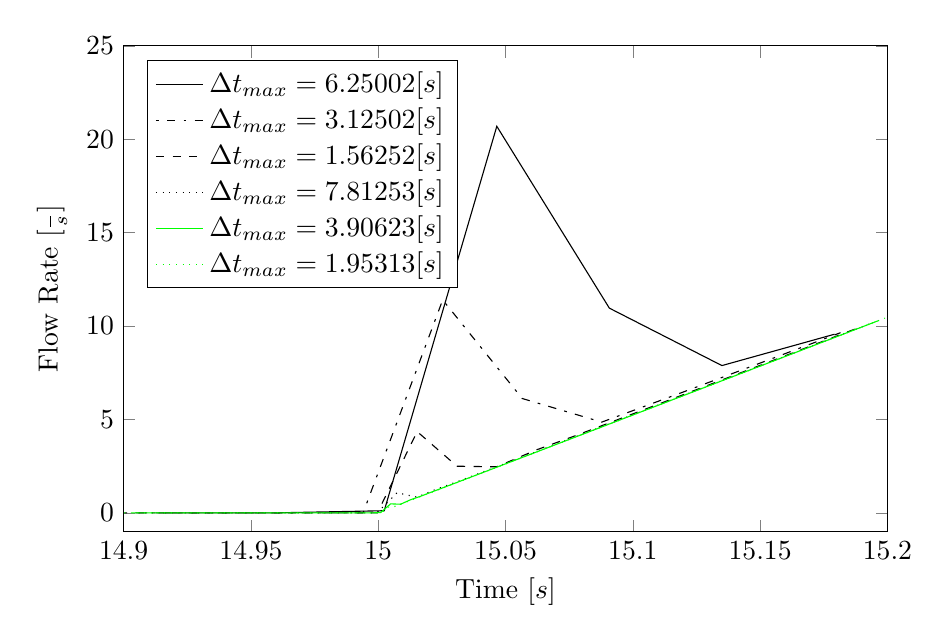
\begin{tikzpicture}

\begin{axis}[%
width=0.8\textwidth,
height=0.508815326102268\textwidth,
scale only axis,
xmin=14.9,
xmax=15.2,
xlabel={Time $[\text{s}]$},
ymin=-1,
ymax=25,
ylabel={Flow Rate $[ \frac{\lbm{}}{\text{s}} ]$},
legend style={at={(0.03,0.97)},anchor=north west,draw=black,fill=white,legend cell align=left}
]
\addplot [
color=black,
solid
]
table[row sep=crcr]{
14.9139289855957 0\\
14.95814037323 0\\
15.0023508071899 0.117176152765751\\
15.0465621948242 20.6927852630615\\
15.0907726287842 10.9598197937012\\
15.1349840164185 7.8855185508728\\
15.1791944503784 9.56354999542236\\
};
\addlegendentry{$\Delta t_{\text{max}} = \expneg{6.2500}{2}{[\text{s}]}$};

\addplot [
color=black,
dash pattern=on 1pt off 3pt on 3pt off 3pt
]
table[row sep=crcr]{
14.9003047943115 0\\
14.9315547943115 0\\
14.9628047943115 0\\
14.9940547943115 0\\
15.0253047943115 11.3998517990112\\
15.0565547943115 6.12321281433105\\
15.0878047943115 4.86077785491943\\
15.1190547943115 6.43307399749756\\
15.1503047943115 8.03494358062744\\
15.1815547943115 9.64548206329346\\
};
\addlegendentry{$\Delta t_{\text{max}} = \expneg{3.1250}{2}{[\text{s}]}$};

\addplot [
color=black,
dashed
]
table[row sep=crcr]{
14.9059162139893 0\\
14.9215412139893 0\\
14.9371662139893 0\\
14.9527912139893 0\\
14.9684162139893 0\\
14.9840412139893 0\\
14.9996662139893 0\\
15.0152912139893 4.35183334350586\\
15.0309162139893 2.5003821849823\\
15.0465412139893 2.46754384040833\\
15.0621662139893 3.37599349021912\\
15.0777912139893 4.14937353134155\\
15.0934162139893 4.95952749252319\\
15.1090412139893 5.76840353012085\\
15.1246662139893 6.57980585098267\\
15.1402912139893 7.39263677597046\\
15.1559162139893 8.20651435852051\\
15.1715412139893 9.02116870880127\\
15.1871662139893 9.83641147613525\\
};
\addlegendentry{$\Delta t_{\text{max}} = \expneg{1.5625}{2}{[\text{s}]}$};

\addplot [
color=black,
dotted
]
table[row sep=crcr]{
14.905800819397 0\\
14.913613319397 0\\
14.921425819397 0\\
14.929238319397 0\\
14.937050819397 0\\
14.944863319397 0\\
14.952675819397 0\\
14.960488319397 0\\
14.968300819397 0\\
14.976113319397 0\\
14.983925819397 0\\
14.991738319397 0\\
14.999550819397 0\\
15.007363319397 1.08051860332489\\
15.015175819397 0.843475759029388\\
15.022988319397 1.2797132730484\\
15.030800819397 1.65828990936279\\
15.038613319397 2.06254577636719\\
15.046425819397 2.46494197845459\\
15.054238319397 2.86959600448608\\
15.062050819397 3.27524924278259\\
15.069863319397 3.68164348602295\\
15.077675819397 4.08856630325317\\
15.085488319397 4.49588108062744\\
15.093300819397 4.90349340438843\\
15.101113319397 5.3113374710083\\
15.108925819397 5.71936464309692\\
15.116738319397 6.12753915786743\\
15.124550819397 6.53583431243896\\
15.132363319397 6.9442286491394\\
15.140175819397 7.35270643234253\\
15.147988319397 7.76125431060791\\
15.155800819397 8.16986179351807\\
15.163613319397 8.57852077484131\\
15.171425819397 8.98722457885742\\
15.179238319397 9.39596652984619\\
15.187050819397 9.80474185943604\\
15.194863319397 10.213547706604\\
};
\addlegendentry{$\Delta t_{\text{max}} = \expneg{7.8125}{3}{[\text{s}]}$};

\addplot [
color=green,
solid
]
table[row sep=crcr]{
14.9033002853394 0\\
14.9072065353394 0\\
14.9111127853394 0\\
14.9150190353394 0\\
14.9189252853394 0\\
14.9228315353394 0\\
14.9267377853394 0\\
14.9306440353394 0\\
14.9345502853394 0\\
14.9384565353394 0\\
14.9423627853394 0\\
14.946268081665 0\\
14.950174331665 0\\
14.954080581665 0\\
14.957986831665 0\\
14.961893081665 0\\
14.965799331665 0\\
14.969705581665 0\\
14.973611831665 0\\
14.977518081665 0\\
14.981424331665 0\\
14.985330581665 0\\
14.989236831665 0\\
14.993143081665 0\\
14.997049331665 0\\
15.000955581665 0.0193258170038462\\
15.004861831665 0.484909266233444\\
15.008768081665 0.465420067310333\\
15.012674331665 0.704263806343079\\
15.016580581665 0.888620138168335\\
15.0204858779907 1.09210002422333\\
15.0243921279907 1.29347014427185\\
15.0282983779907 1.49598813056946\\
15.0322046279907 1.69893610477448\\
15.0361108779907 1.90221953392029\\
15.0400171279907 2.1057436466217\\
15.0439233779907 2.30944752693176\\
15.0478296279907 2.51328921318054\\
15.0517358779907 2.7172384262085\\
15.0556421279907 2.92127346992493\\
15.0595483779907 3.12537741661072\\
15.0634546279907 3.32953834533691\\
15.0673608779907 3.53374648094177\\
15.0712671279907 3.73799395561218\\
15.0751733779907 3.94227480888367\\
15.0790796279907 4.14658403396606\\
15.0829858779907 4.35091829299927\\
15.0868921279907 4.55527353286743\\
15.0907983779907 4.75964736938477\\
15.0947036743164 4.96403741836548\\
15.0986099243164 5.16844177246094\\
15.1025161743164 5.37285900115967\\
15.1064224243164 5.5772876739502\\
15.1103286743164 5.78172636032104\\
15.1142349243164 5.9861741065979\\
15.1181411743164 6.1906304359436\\
15.1220474243164 6.39509391784668\\
15.1259536743164 6.59956407546997\\
15.1298599243164 6.80404043197632\\
15.1337661743164 7.00852251052856\\
15.1376724243164 7.21300935745239\\
15.1415786743164 7.41750144958496\\
15.1454849243164 7.62199735641479\\
15.1493911743164 7.82649755477905\\
15.1532974243164 8.03100109100342\\
15.1572036743164 8.23550891876221\\
15.1611099243164 8.44001865386963\\
15.1650161743164 8.64453220367432\\
15.1689214706421 8.84904861450195\\
15.1728277206421 9.05356693267822\\
15.1767339706421 9.25808811187744\\
15.1806402206421 9.46261119842529\\
15.1845464706421 9.66713619232178\\
15.1884527206421 9.87166404724121\\
15.1923589706421 10.076192855835\\
15.1962652206421 10.2807235717773\\
};
\addlegendentry{$\Delta t_{\text{max}} = \expneg{3.9062}{3}{[\text{s}]}$};

\addplot [
color=green,
dotted
]
table[row sep=crcr]{
14.900221824646 0\\
14.902174949646 0\\
14.904128074646 0\\
14.906081199646 0\\
14.908034324646 0\\
14.909987449646 0\\
14.911940574646 0\\
14.913893699646 0\\
14.915846824646 0\\
14.9177989959717 0\\
14.9197521209717 0\\
14.9217052459717 0\\
14.9236583709717 0\\
14.9256114959717 0\\
14.9275646209717 0\\
14.9295177459717 0\\
14.9314708709717 0\\
14.9334239959717 0\\
14.9353771209717 0\\
14.9373302459717 0\\
14.9392833709717 0\\
14.9412364959717 0\\
14.9431896209717 0\\
14.9451427459717 0\\
14.9470958709717 0\\
14.9490489959717 0\\
14.9510021209717 0\\
14.9529552459717 0\\
14.9549083709717 0\\
14.9568614959717 0\\
14.9588146209717 0\\
14.9607677459717 0\\
14.9627208709717 0\\
14.9646739959717 0\\
14.9666271209717 0\\
14.9685802459717 0\\
14.9705333709717 0\\
14.9724864959717 0\\
14.9744396209717 0\\
14.9763927459717 0\\
14.9783458709717 0\\
14.9802989959717 0\\
14.9822521209717 0\\
14.9842052459717 0\\
14.9861583709717 0\\
14.9881114959717 0\\
14.9900646209717 0\\
14.9920167922974 0\\
14.9939699172974 0\\
14.9959230422974 0\\
14.9978761672974 0\\
14.9998292922974 0\\
15.0017824172974 0.0664489343762398\\
15.0037355422974 0.311820924282074\\
15.0056886672974 0.301760196685791\\
15.0076417922974 0.415858924388886\\
15.0095949172974 0.511866450309753\\
15.0115480422974 0.613315761089325\\
15.0135011672974 0.714363992214203\\
15.0154542922974 0.815780222415924\\
15.0174074172974 0.917371690273285\\
15.0193605422974 1.01909780502319\\
15.0213136672974 1.12092268466949\\
15.0232667922974 1.22282266616821\\
15.0252199172974 1.32478082180023\\
15.0271730422974 1.42678511142731\\
15.0291261672974 1.52882647514343\\
15.0310792922974 1.6308981180191\\
15.0330324172974 1.73299479484558\\
15.0349855422974 1.83511233329773\\
15.0369386672974 1.93724751472473\\
15.0388917922974 2.03939771652222\\
15.0408449172974 2.14156079292297\\
15.0427980422974 2.24373507499695\\
15.0447511672974 2.34591913223267\\
15.0467042922974 2.44811153411865\\
15.0486574172974 2.55031156539917\\
15.0506105422974 2.65251803398132\\
15.0525636672974 2.75473070144653\\
15.0545167922974 2.8569483757019\\
15.0564699172974 2.95917081832886\\
15.0584230422974 3.06139755249023\\
15.0603761672974 3.16362810134888\\
15.0623292922974 3.26586222648621\\
15.0642824172974 3.36809945106506\\
15.066234588623 3.47033953666687\\
15.068187713623 3.57258224487305\\
15.070140838623 3.67482733726501\\
15.072093963623 3.77707481384277\\
15.074047088623 3.87932419776917\\
15.076000213623 3.98157548904419\\
15.077953338623 4.08382844924927\\
15.079906463623 4.18608331680298\\
15.081859588623 4.28833961486816\\
15.083812713623 4.39059734344482\\
15.085765838623 4.4928560256958\\
15.087718963623 4.59511613845825\\
15.089672088623 4.69737720489502\\
15.091625213623 4.79963970184326\\
15.093578338623 4.90190315246582\\
15.095531463623 5.0041675567627\\
15.097484588623 5.10643243789673\\
15.099437713623 5.20869874954224\\
15.101390838623 5.31096506118774\\
15.103343963623 5.41323280334473\\
15.105297088623 5.51550102233887\\
15.107250213623 5.61776971817017\\
15.109203338623 5.72003936767578\\
15.111156463623 5.82230949401855\\
15.113109588623 5.92458009719849\\
15.115062713623 6.02685117721558\\
15.117015838623 6.12912273406982\\
15.118968963623 6.23139524459839\\
15.120922088623 6.33366775512695\\
15.122875213623 6.43594074249268\\
15.124828338623 6.53821420669556\\
15.126781463623 6.6404881477356\\
15.128734588623 6.74276208877563\\
15.130687713623 6.84503698348999\\
15.132640838623 6.94731187820435\\
15.134593963623 7.04958724975586\\
15.136547088623 7.15186262130737\\
15.138500213623 7.25413846969604\\
15.1404523849487 7.35641479492188\\
15.1424055099487 7.45869112014771\\
15.1443586349487 7.56096792221069\\
15.1463117599487 7.66324472427368\\
15.1482648849487 7.76552200317383\\
15.1502180099487 7.86779975891113\\
15.1521711349487 7.97007703781128\\
15.1541242599487 8.07235527038574\\
15.1560773849487 8.17463302612305\\
15.1580305099487 8.27691173553467\\
15.1599836349487 8.37919044494629\\
15.1619367599487 8.48146915435791\\
15.1638898849487 8.58374786376953\\
15.1658430099487 8.68602657318115\\
15.1677961349487 8.78830623626709\\
15.1697492599487 8.89058494567871\\
15.1717023849487 8.99286460876465\\
15.1736555099487 9.09514427185059\\
15.1756086349487 9.19742393493652\\
15.1775617599487 9.29970455169678\\
15.1795148849487 9.40198421478271\\
15.1814680099487 9.50426483154297\\
15.1834211349487 9.60654544830322\\
15.1853742599487 9.70882511138916\\
15.1873273849487 9.81110572814941\\
15.1892805099487 9.91338729858398\\
15.1912336349487 10.0156679153442\\
15.1931867599487 10.1179485321045\\
15.1951398849487 10.2202301025391\\
15.1970930099487 10.3225107192993\\
15.1990461349487 10.4247922897339\\
};
\addlegendentry{$\Delta t_{\text{max}} = \expneg{1.9531}{3}{[\text{s}]}$};

\end{axis}
\end{tikzpicture}%
\label{fig:valveLinSols}
\caption{Zoom of flow rate in linear solutions to the valve problem.}
\end{figure}

The presence of the spike in the flow rate in the simulation with \dtmax{} = \expneg{1.56}{2}{[2]}, a \dtmax{} that produces a \dt{} history that is never \dtcrnt{} limited, necessitated that additional timestep refinements be examined for a smooth solution.
Subsequent timestep refinements produced results where the flow-rate spikes became progressively smaller; however, the time-step refinement study did not yield a solution that did not have this perturbation.
The lack of a linear solution that is free from is not an impediment to this study since the purpose is not to find a \dtmax{} that produces such a solution.
Instead \tab{tab:valveLinDataTable} shows the run time statistics for the linear solver's solutions.

\begin{table}[h!t]
\centering
\singlespace
\pgfplotstabletypeset[sci zerofill,sci E, col sep=comma,
	columns/0/.style={ column name= $[ \text{s} ]$, precision=1},
	columns/1/.style={ column name= $[ - ]$, int detect},
	columns/2/.style={ column name= $[ \text{s} ]$, precision=3},
	columns/3/.style={ column name= $[ \text{s} ]$, precision=3},
	every head row/.style={
		before row={
			\toprule
			\dtmax{} & $N_{t}$ & $T_{\text{CPU}}$& $\frac{T_{\text{CPU}}}{N_{t}}$ \\
		},
		after row=\midrule
	},
	every last row/.style={
after row=\bottomrule}]{tables/valveLinData.tex}

\caption{Rum time data for the valve problem using the linear solver.}
\label{tab:valveLinDataTable}
\end{table}

In \tab{tab:valveLinDataTable} the first column shows the maximum timestep size for the simulation.
The second column shows the number of successful timesteps taken, $N_{t}$.
The third column is the cpu time required to complete simulation, $T_{\text{CPU}}$.
The final column is the the cpu time per timestep for a given simulation.
On average, the cpu time per timestep is \expneg{2.8}{3}{[s]} for the linear solution.

Next, the nonlinear solver was used to perform the same timestep sensitivity study.
The same set of \dtmax{} were run.
The solution at \dtmax{} = \expneg{6.25}{2}{[s]} is shown in \fig{fig:valveNln6pt25em02}

\begin{figure}[h!t]
\centering
% This file was created by matlab2tikz v0.4.3.
% Copyright (c) 2008--2013, Nico Schlömer <nico.schloemer@gmail.com>
% All rights reserved.
% 
\tikzsetnextfilename{plots/valveNln6pt2500em02_eps}
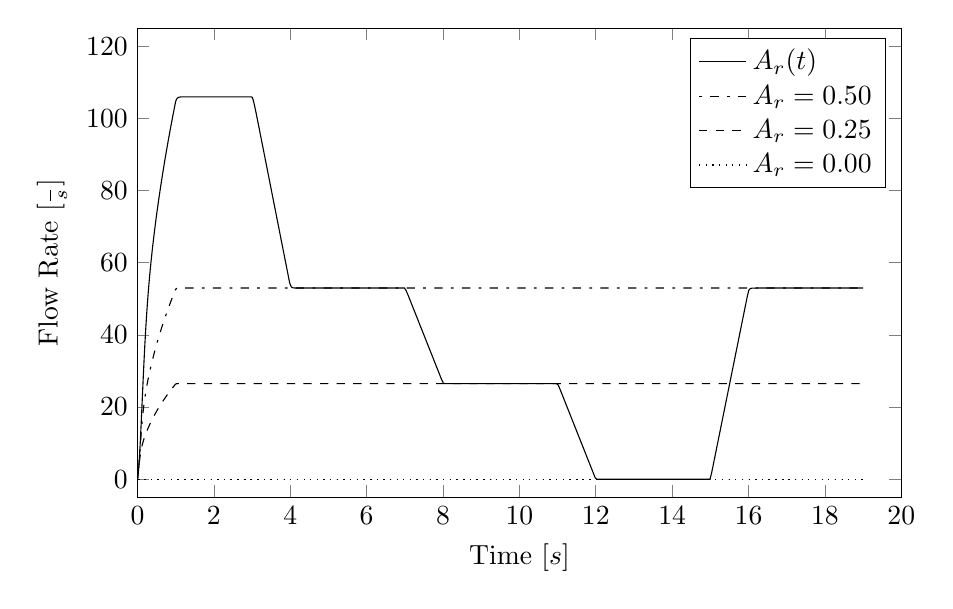
\begin{tikzpicture}

\begin{axis}[%
width=0.8\textwidth,
%height=0.630967741935484\textwidth,
height=0.491294629700995\textwidth,
scale only axis,
xmin=0,
xmax=20,
xlabel={Time $[\text{s}]$},
ymin=-5,
ymax=125,
ylabel={Flow Rate $[ \frac{\lbm{}}{\text{s}} ]$},
legend style={draw=black,fill=white,legend cell align=left}
]
\addplot [
color=black,
solid
]
table[row sep=crcr]{
0 0\\
9.99999974737875e-06 -2.68723052698761e-08\\
2.49999993684469e-05 5.97379596456449e-07\\
4.75000015285332e-05 1.5992671251297e-05\\
8.12500002211891e-05 0.000229224911890924\\
0.000131875000079162 0.00192544842138886\\
0.000207812496228144 0.00898910593241453\\
0.000321718747727573 0.0234754215925932\\
0.000492578139528632 0.0383502058684826\\
0.00074886716902256 0.0502719767391682\\
0.00113330082967877 0.0704958811402321\\
0.00170995120424777 0.108530916273594\\
0.00257492670789361 0.167750313878059\\
0.00387239013798535 0.258952885866165\\
0.00529959984123707 0.363639861345291\\
0.00686953077092767 0.484229981899261\\
0.0085964547470212 0.623396694660187\\
0.0104960706084967 0.784338176250458\\
0.0125856483355165 0.970849931240082\\
0.014884184114635 1.18742954730988\\
0.0174125730991364 1.43940579891205\\
0.020193800330162 1.73308956623077\\
0.0232531521469355 2.07594513893127\\
0.0266184378415346 2.4767849445343\\
0.0303202513605356 2.94598364830017\\
0.0343922488391399 3.49570560455322\\
0.0388714447617531 4.14013338088989\\
0.0437985584139824 4.89567756652832\\
0.0492183864116669 5.78112745285034\\
0.0551801957190037 6.81768989562988\\
0.0617381855845451 8.02883529663086\\
0.0689519718289375 9.43983745574951\\
0.0768871381878853 11.0768632888794\\
0.0856158286333084 12.9654607772827\\
0.095217376947403 15.1283092498779\\
0.105779089033604 17.5821762084961\\
0.117396965622902 20.3342571258545\\
0.13017663359642 23.3783740997314\\
0.144234269857407 26.6919059753418\\
0.159697666764259 30.2346706390381\\
0.176707401871681 33.9509391784668\\
0.195418119430542 37.7751693725586\\
0.215999901294708 41.6409111022949\\
0.238639861345291 45.4909553527832\\
0.2635438144207 49.2860527038574\\
0.290938168764114 53.0097274780273\\
0.321071952581406 56.6680793762207\\
0.354219108819962 60.2851753234863\\
0.390680998563766 63.8959426879883\\
0.427134186029434 67.2247619628906\\
0.461836785078049 70.1926651000977\\
0.495115727186203 72.8892974853516\\
0.527189493179321 75.372917175293\\
0.558222532272339 77.6839752197266\\
0.588342726230621 79.8516006469727\\
0.617652356624603 81.8974990844727\\
0.646234631538391 83.8383636474609\\
0.674158751964569 85.6873397827148\\
0.701483011245728 87.4550094604492\\
0.728256940841675 89.1500778198242\\
0.754523456096649 90.77978515625\\
0.780319631099701 92.3502655029297\\
0.805678188800812 93.8667373657227\\
0.830627858638763 95.3337249755859\\
0.855194389820099 96.7551498413086\\
0.879400551319122 98.1344680786133\\
0.903267025947571 99.4747085571289\\
0.926812350749969 100.778564453125\\
0.950053453445435 102.048461914063\\
0.973005652427673 103.286552429199\\
0.995683073997498 104.494781494141\\
1.01809847354889 105.217460632324\\
1.0402637720108 105.585472106934\\
1.06237816810608 105.774543762207\\
1.08448839187622 105.871826171875\\
1.10659623146057 105.921867370605\\
1.12870299816132 105.947608947754\\
1.15080916881561 105.960845947266\\
1.17291498184204 105.967651367188\\
1.19502067565918 105.971153259277\\
1.21712636947632 105.972946166992\\
1.23923194408417 105.973876953125\\
1.26133751869202 105.974349975586\\
1.28344309329987 105.974594116211\\
1.30554866790771 105.974716186523\\
1.32765424251556 105.974784851074\\
1.34975969791412 105.974815368652\\
1.37186527252197 105.974830627441\\
1.39397084712982 105.974838256836\\
1.41607642173767 105.97484588623\\
1.43818199634552 105.97484588623\\
1.46028745174408 105.974853515625\\
1.48239302635193 105.974853515625\\
1.50449860095978 105.974853515625\\
1.52660417556763 105.974853515625\\
1.54870975017548 105.974853515625\\
1.57081520557404 105.974853515625\\
1.59292078018188 105.974853515625\\
1.61502635478973 105.974853515625\\
1.63713192939758 105.974853515625\\
1.65923750400543 105.974853515625\\
1.68134295940399 105.974853515625\\
1.70344853401184 105.974853515625\\
1.72555410861969 105.974853515625\\
1.74765968322754 105.974853515625\\
1.76976525783539 105.974853515625\\
1.79187071323395 105.974853515625\\
1.8139762878418 105.974853515625\\
1.83608186244965 105.974853515625\\
1.8581874370575 105.974853515625\\
1.88029301166534 105.974853515625\\
1.9023984670639 105.974853515625\\
1.92450404167175 105.974853515625\\
1.9466096162796 105.974853515625\\
1.96871519088745 105.974853515625\\
1.9908207654953 105.974853515625\\
2.01292634010315 105.974853515625\\
2.03503179550171 105.974853515625\\
2.05713748931885 105.974853515625\\
2.07924294471741 105.974853515625\\
2.10134840011597 105.974853515625\\
2.12345409393311 105.974853515625\\
2.14555954933167 105.974853515625\\
2.1676652431488 105.974853515625\\
2.18977069854736 105.974853515625\\
2.21187615394592 105.974853515625\\
2.23398184776306 105.974853515625\\
2.25608730316162 105.974853515625\\
2.27819299697876 105.974853515625\\
2.30029845237732 105.974853515625\\
2.32240390777588 105.974853515625\\
2.34450960159302 105.974853515625\\
2.36661505699158 105.974853515625\\
2.38872075080872 105.974853515625\\
2.41082620620728 105.974853515625\\
2.43293166160584 105.974853515625\\
2.45503735542297 105.974853515625\\
2.47714281082153 105.974853515625\\
2.49924850463867 105.974853515625\\
2.52135396003723 105.974853515625\\
2.54345941543579 105.974853515625\\
2.56556510925293 105.974853515625\\
2.58767056465149 105.974853515625\\
2.60977625846863 105.974853515625\\
2.63188171386719 105.974853515625\\
2.65398716926575 105.974853515625\\
2.67609286308289 105.974853515625\\
2.69819831848145 105.974853515625\\
2.72030401229858 105.974853515625\\
2.74240946769714 105.974853515625\\
2.7645149230957 105.974853515625\\
2.78662061691284 105.974853515625\\
2.8087260723114 105.974853515625\\
2.83083176612854 105.974853515625\\
2.8529372215271 105.974853515625\\
2.87504267692566 105.974853515625\\
2.8971483707428 105.974853515625\\
2.91925382614136 105.974853515625\\
2.9413595199585 105.974853515625\\
2.96346497535706 105.974853515625\\
2.98557043075562 105.974853515625\\
3.00767612457275 105.776901245117\\
3.02978157997131 105.100280761719\\
3.0519700050354 104.171333312988\\
3.07440447807312 103.101539611816\\
3.09709739685059 101.951995849609\\
3.12005996704102 100.754364013672\\
3.14330291748047 99.5247421264648\\
3.166836977005 98.2710571289063\\
3.19067335128784 96.9970169067383\\
3.21482396125793 95.7041015625\\
3.2393012046814 94.392707824707\\
3.26411890983582 93.0626068115234\\
3.28929138183594 91.7132720947266\\
3.31483387947083 90.3440017700195\\
3.34076333045959 88.9539413452148\\
3.36709761619568 87.5421447753906\\
3.39385652542114 86.1075820922852\\
3.42106103897095 84.6491241455078\\
3.44873404502869 83.1655502319336\\
3.47690057754517 81.6555328369141\\
3.50558733940125 80.1175994873047\\
3.53482460975647 78.550163269043\\
3.5646448135376 76.9514770507813\\
3.59508395195007 75.3195953369141\\
3.62618231773376 73.6523895263672\\
3.65798377990723 71.9474716186523\\
3.69053816795349 70.2022018432617\\
3.72390079498291 68.4135818481445\\
3.75813484191895 66.5782623291016\\
3.79331135749817 64.6924133300781\\
3.82951164245605 62.7516708374023\\
3.86682963371277 60.7510070800781\\
3.90537428855896 58.6845817565918\\
3.94527339935303 56.5455436706543\\
3.98667812347412 54.3257865905762\\
4.02976989746094 53.2729530334473\\
4.07350301742554 53.0479316711426\\
4.11750602722168 53.0003852844238\\
4.16167545318604 52.9903907775879\\
4.2058801651001 52.9882926940918\\
4.2500901222229 52.9878540039063\\
4.29430055618286 52.9877624511719\\
4.33851099014282 52.9877433776855\\
4.38272142410278 52.9877395629883\\
4.4269323348999 52.9877395629883\\
4.47114324569702 52.9877395629883\\
4.51535367965698 52.9877395629883\\
4.5595645904541 52.9877395629883\\
4.60377550125122 52.9877395629883\\
4.64798641204834 52.9877395629883\\
4.69219732284546 52.9877395629883\\
4.73640823364258 52.9877395629883\\
4.7806191444397 52.9877395629883\\
4.82482957839966 52.9877395629883\\
4.86904048919678 52.9877395629883\\
4.9132513999939 52.9877395629883\\
4.95746231079102 52.9877395629883\\
5.00167322158813 52.9877395629883\\
5.04588413238525 52.9877395629883\\
5.09009504318237 52.9877395629883\\
5.13430547714233 52.9877395629883\\
5.17851638793945 52.9877395629883\\
5.22272729873657 52.9877395629883\\
5.26693820953369 52.9877395629883\\
5.31114912033081 52.9877395629883\\
5.35536003112793 52.9877395629883\\
5.39957046508789 52.9877395629883\\
5.44378137588501 52.9877395629883\\
5.48799228668213 52.9877395629883\\
5.53220319747925 52.9877395629883\\
5.57641410827637 52.9877395629883\\
5.62062501907349 52.9877395629883\\
5.66483592987061 52.9877395629883\\
5.70904636383057 52.9877395629883\\
5.75325727462769 52.9877395629883\\
5.7974681854248 52.9877395629883\\
5.84167909622192 52.9877395629883\\
5.88589000701904 52.9877395629883\\
5.93010091781616 52.9877395629883\\
5.97431182861328 52.9877395629883\\
6.01852226257324 52.9877395629883\\
6.06273317337036 52.9877395629883\\
6.10694408416748 52.9877395629883\\
6.1511549949646 52.9877395629883\\
6.19536590576172 52.9877395629883\\
6.23957681655884 52.9877395629883\\
6.28378772735596 52.9877395629883\\
6.32799816131592 52.9877395629883\\
6.37220907211304 52.9877395629883\\
6.41641998291016 52.9877395629883\\
6.46063089370728 52.9877395629883\\
6.50484180450439 52.9877395629883\\
6.54905271530151 52.9877395629883\\
6.59326362609863 52.9877395629883\\
6.63747406005859 52.9877395629883\\
6.68168497085571 52.9877395629883\\
6.72589588165283 52.9877395629883\\
6.77010679244995 52.9877395629883\\
6.81431770324707 52.9877395629883\\
6.85852861404419 52.9877395629883\\
6.90273904800415 52.9877395629883\\
6.94694995880127 52.9877395629883\\
6.99116086959839 52.9877395629883\\
7.03537178039551 52.2437324523926\\
7.07958269119263 51.1552505493164\\
7.12379360198975 49.995246887207\\
7.16800451278687 48.8206787109375\\
7.21221494674683 47.643196105957\\
7.25642585754395 46.465145111084\\
7.30063676834106 45.286979675293\\
7.34484767913818 44.1087989807129\\
7.3890585899353 42.9306106567383\\
7.43326950073242 41.7524223327637\\
7.47748041152954 40.5742340087891\\
7.5216908454895 39.3960456848145\\
7.56590175628662 38.2178573608398\\
7.61011266708374 37.039665222168\\
7.65432357788086 35.8614768981934\\
7.69853448867798 34.6832847595215\\
7.7427453994751 33.5050964355469\\
7.78695631027222 32.326904296875\\
7.83116674423218 31.1487159729004\\
7.8753776550293 29.9705257415771\\
7.91958856582642 28.7923336029053\\
7.96379947662354 27.614143371582\\
8.0080099105835 26.624584197998\\
8.05222129821777 26.5094051361084\\
8.09643173217773 26.495719909668\\
8.14064311981201 26.4941215515137\\
8.18485355377197 26.4939346313477\\
8.22906494140625 26.4939117431641\\
8.27327537536621 26.4939098358154\\
8.31748580932617 26.4939098358154\\
8.36169719696045 26.4939079284668\\
8.40590763092041 26.4939079284668\\
8.45011901855469 26.4939079284668\\
8.49432945251465 26.4939079284668\\
8.53854084014893 26.4939079284668\\
8.58275127410889 26.4939079284668\\
8.62696170806885 26.4939079284668\\
8.67117309570313 26.4939079284668\\
8.71538352966309 26.4939079284668\\
8.75959491729736 26.4939079284668\\
8.80380535125732 26.4939079284668\\
8.8480167388916 26.4939079284668\\
8.89222717285156 26.4939079284668\\
8.93643760681152 26.4939079284668\\
8.9806489944458 26.4939079284668\\
9.02485942840576 26.4939079284668\\
9.06907081604004 26.4939079284668\\
9.11328125 26.4939079284668\\
9.15749168395996 26.4939079284668\\
9.20170307159424 26.4939079284668\\
9.2459135055542 26.4939079284668\\
9.29012489318848 26.4939079284668\\
9.33433532714844 26.4939079284668\\
9.37854671478271 26.4939079284668\\
9.42275714874268 26.4939079284668\\
9.46696758270264 26.4939079284668\\
9.51117897033691 26.4939079284668\\
9.55538940429688 26.4939079284668\\
9.59960079193115 26.4939079284668\\
9.64381122589111 26.4939079284668\\
9.68802261352539 26.4939079284668\\
9.73223304748535 26.4939079284668\\
9.77644348144531 26.4939079284668\\
9.82065486907959 26.4939079284668\\
9.86486530303955 26.4939079284668\\
9.90907669067383 26.4939079284668\\
9.95328712463379 26.4939079284668\\
9.99749851226807 26.4939079284668\\
10.041708946228 26.4939079284668\\
10.085919380188 26.4939079284668\\
10.1301307678223 26.4939079284668\\
10.1743412017822 26.4939079284668\\
10.2185525894165 26.4939079284668\\
10.2627630233765 26.4939079284668\\
10.3069744110107 26.4939079284668\\
10.3511848449707 26.4939079284668\\
10.3953952789307 26.4939079284668\\
10.4396066665649 26.4939079284668\\
10.4838171005249 26.4939079284668\\
10.5280284881592 26.4939079284668\\
10.5722389221191 26.4939079284668\\
10.6164503097534 26.4939079284668\\
10.6606607437134 26.4939079284668\\
10.7048711776733 26.4939079284668\\
10.7490825653076 26.4939079284668\\
10.7932929992676 26.4939079284668\\
10.8375043869019 26.4939079284668\\
10.8817148208618 26.4939079284668\\
10.9259262084961 26.4939079284668\\
10.9701366424561 26.4939079284668\\
11.014347076416 26.1576271057129\\
11.0585584640503 25.0768013000488\\
11.1027688980103 23.90940284729\\
11.1469802856445 22.7323703765869\\
11.1911907196045 21.5542984008789\\
11.2354021072388 20.3761215209961\\
11.2796125411987 19.1979331970215\\
11.3238229751587 18.0197467803955\\
11.368034362793 16.8415603637695\\
11.4122447967529 15.6633768081665\\
11.4561223983765 14.4940776824951\\
11.5 13.3247852325439\\
11.54421043396 12.14661693573\\
11.5884218215942 10.9684581756592\\
11.6326322555542 9.79013824462891\\
11.6768436431885 8.61193943023682\\
11.7210540771484 7.43374538421631\\
11.7652654647827 6.25555229187012\\
11.8094758987427 5.07735872268677\\
11.8536863327026 3.89916563034058\\
11.8978977203369 2.72097659111023\\
11.9421081542969 1.54277789592743\\
11.9863195419312 0.36458432674408\\
12.0305299758911 0\\
12.0747413635254 0\\
12.1189517974854 0\\
12.1631622314453 0\\
12.2073736190796 0\\
12.2515840530396 0\\
12.2957954406738 0\\
12.3400058746338 0\\
12.3842172622681 0\\
12.428427696228 0\\
12.472638130188 0\\
12.5168495178223 0\\
12.5610599517822 0\\
12.6052713394165 0\\
12.6494817733765 0\\
12.6936931610107 0\\
12.7379035949707 0\\
12.7821140289307 0\\
12.8263254165649 0\\
12.8705358505249 0\\
12.9147472381592 0\\
12.9589576721191 0\\
13.0031690597534 0\\
13.0473794937134 0\\
13.0915899276733 0\\
13.1358013153076 0\\
13.1800117492676 0\\
13.2242231369019 0\\
13.2684335708618 0\\
13.3126440048218 0\\
13.3568553924561 0\\
13.401065826416 0\\
13.4452772140503 0\\
13.4894876480103 0\\
13.5336990356445 0\\
13.5779094696045 0\\
13.6221199035645 0\\
13.6663312911987 0\\
13.7105417251587 0\\
13.754753112793 0\\
13.7989635467529 0\\
13.8431749343872 0\\
13.8873853683472 0\\
13.9315958023071 0\\
13.9758071899414 0\\
14.0200176239014 0\\
14.0642290115356 0\\
14.1084394454956 0\\
14.1526508331299 0\\
14.1968612670898 0\\
14.2410717010498 0\\
14.2852830886841 0\\
14.329493522644 0\\
14.3737049102783 0\\
14.4179153442383 0\\
14.4621267318726 0\\
14.5063371658325 0\\
14.5505475997925 0\\
14.5947589874268 0\\
14.6389694213867 0\\
14.683180809021 0\\
14.727391242981 0\\
14.7716026306152 0\\
14.8158130645752 0\\
14.8600234985352 0\\
14.9042348861694 0\\
14.9484453201294 0\\
14.9926567077637 0\\
15.0368671417236 1.93454301357269\\
15.0810785293579 4.24624395370483\\
15.1252889633179 6.56158781051636\\
15.1694993972778 8.87692451477051\\
15.2137107849121 11.1922979354858\\
15.2579212188721 13.5076742172241\\
15.3021326065063 15.8230504989624\\
15.3463430404663 18.1384258270264\\
15.3905544281006 20.4538021087646\\
15.4347648620605 22.7691783905029\\
15.4789752960205 25.0845527648926\\
15.5231866836548 27.3999271392822\\
15.5673971176147 29.7153015136719\\
15.611608505249 32.0306739807129\\
15.655818939209 34.3460464477539\\
15.7000303268433 36.6614189147949\\
15.7442407608032 38.9767913818359\\
15.7884511947632 41.2921600341797\\
15.8326625823975 43.6075286865234\\
15.8768730163574 45.9228973388672\\
15.9210844039917 48.2382850646973\\
15.9652948379517 50.5536499023438\\
16.0095062255859 52.4762725830078\\
16.0537166595459 52.8805809020996\\
16.0967807769775 52.9648361206055\\
16.1407527923584 52.9829216003418\\
16.1849117279053 52.9867286682129\\
16.2291107177734 52.9875259399414\\
16.2733192443848 52.9876937866211\\
16.3175296783447 52.9877281188965\\
16.3617401123047 52.987735748291\\
16.4059524536133 52.9877395629883\\
16.4501628875732 52.9877395629883\\
16.4943733215332 52.9877395629883\\
16.5385837554932 52.9877395629883\\
16.5827941894531 52.9877395629883\\
16.6270065307617 52.9877395629883\\
16.6712169647217 52.9877395629883\\
16.7154273986816 52.9877395629883\\
16.7596378326416 52.9877395629883\\
16.8038482666016 52.9877395629883\\
16.8480606079102 52.9877395629883\\
16.8922710418701 52.9877395629883\\
16.9364814758301 52.9877395629883\\
16.98069190979 52.9877395629883\\
17.0249042510986 52.9877395629883\\
17.0691146850586 52.9877395629883\\
17.1133251190186 52.9877395629883\\
17.1575355529785 52.9877395629883\\
17.2017459869385 52.9877395629883\\
17.2459583282471 52.9877395629883\\
17.290168762207 52.9877395629883\\
17.334379196167 52.9877395629883\\
17.378589630127 52.9877395629883\\
17.4228000640869 52.9877395629883\\
17.4670124053955 52.9877395629883\\
17.5112228393555 52.9877395629883\\
17.5554332733154 52.9877395629883\\
17.5996437072754 52.9877395629883\\
17.643856048584 52.9877395629883\\
17.6880664825439 52.9877395629883\\
17.7322769165039 52.9877395629883\\
17.7764873504639 52.9877395629883\\
17.8206977844238 52.9877395629883\\
17.8649101257324 52.9877395629883\\
17.9091205596924 52.9877395629883\\
17.9533309936523 52.9877395629883\\
17.9975414276123 52.9877395629883\\
18.0417518615723 52.9877395629883\\
18.0859642028809 52.9877395629883\\
18.1301746368408 52.9877395629883\\
18.1743850708008 52.9877395629883\\
18.2185955047607 52.9877395629883\\
18.2628059387207 52.9877395629883\\
18.3070182800293 52.9877395629883\\
18.3512287139893 52.9877395629883\\
18.3954391479492 52.9877395629883\\
18.4396495819092 52.9877395629883\\
18.4838619232178 52.9877395629883\\
18.5280723571777 52.9877395629883\\
18.5722827911377 52.9877395629883\\
18.6164932250977 52.9877395629883\\
18.6607036590576 52.9877395629883\\
18.7049160003662 52.9877395629883\\
18.7491264343262 52.9877395629883\\
18.7933368682861 52.9877395629883\\
18.8375473022461 52.9877395629883\\
18.8817577362061 52.9877395629883\\
18.9259700775146 52.9877395629883\\
18.962984085083 52.9877395629883\\
19 52.9877395629883\\
};
\addlegendentry{$A_{r}(t)$};

\addplot [
color=black,
dash pattern=on 1pt off 3pt on 3pt off 3pt
]
table[row sep=crcr]{
0 0\\
9.99999974737875e-06 -2.6872250202814e-08\\
2.49999993684469e-05 5.97376981659181e-07\\
4.75000015285332e-05 1.5992558473954e-05\\
8.12500002211891e-05 0.000229222685447894\\
0.000131875000079162 0.00192542537115514\\
0.000207812496228144 0.00898898299783468\\
0.000321718747727573 0.0234750732779503\\
0.000492578139528632 0.0383495762944222\\
0.00074886716902256 0.0502709187567234\\
0.00113330082967877 0.0704936757683754\\
0.00170995120424777 0.10852438211441\\
0.00257492670789361 0.167728826403618\\
0.00387239013798535 0.258878469467163\\
0.00529959984123707 0.36345100402832\\
0.00686953077092767 0.483818382024765\\
0.0085964547470212 0.62257993221283\\
0.0104960706084967 0.782817423343658\\
0.0125856483355165 0.968145906925201\\
0.014884184114635 1.18278455734253\\
0.0174125730991364 1.43163669109344\\
0.020193800330162 1.72036504745483\\
0.0232531521469355 2.05545377731323\\
0.0266184378415346 2.44424080848694\\
0.0303202513605356 2.89489793777466\\
0.0343922488391399 3.41632533073425\\
0.0388714447617531 4.01791954040527\\
0.0437985584139824 4.70916080474854\\
0.0492183864116669 5.49897241592407\\
0.0551801957190037 6.39480876922607\\
0.0617381855845451 7.40148830413818\\
0.0689519718289375 8.51985263824463\\
0.0768871381878853 9.74547004699707\\
0.0856158286333084 11.0677270889282\\
0.095217376947403 12.4697322845459\\
0.105779089033604 13.9294090270996\\
0.117396965622902 15.4219026565552\\
0.13017663359642 16.9229755401611\\
0.144234269857407 18.4126529693604\\
0.159697666764259 19.8781642913818\\
0.176707401871681 21.3153514862061\\
0.195418119430542 22.7282943725586\\
0.215999901294708 24.1273956298828\\
0.238639861345291 25.5267066955566\\
0.2635438144207 26.9412879943848\\
0.290938168764114 28.3852310180664\\
0.321071952581406 29.8706207275391\\
0.354219108819962 31.407299041748\\
0.390680998563766 33.0031890869141\\
0.427134186029434 34.5181922912598\\
0.461836785078049 35.8965759277344\\
0.495115727186203 37.1668472290039\\
0.527189493179321 38.3486099243164\\
0.558222532272339 39.4563026428223\\
0.588342726230621 40.5008735656738\\
0.617652356624603 41.4908561706543\\
0.646234631538391 42.4330406188965\\
0.674158751964569 43.3329467773438\\
0.701483011245728 44.1951179504395\\
0.728256940841675 45.0233535766602\\
0.754523456096649 45.8208694458008\\
0.780319631099701 46.5904159545898\\
0.805678188800812 47.3343620300293\\
0.830627858638763 48.0547714233398\\
0.855194389820099 48.7534446716309\\
0.879400551319122 49.4319801330566\\
0.903267025947571 50.0917816162109\\
0.926812350749969 50.7341117858887\\
0.950053453445435 51.3600959777832\\
0.973005652427673 51.9707489013672\\
0.995683073997498 52.5669860839844\\
1.01809847354889 52.8432464599609\\
1.0402637720108 52.9377632141113\\
1.06237816810608 52.9704170227051\\
1.08448839187622 52.9817276000977\\
1.10659623146057 52.9856491088867\\
1.12870299816132 52.9870109558105\\
1.15080916881561 52.9874839782715\\
1.17291498184204 52.9876518249512\\
1.19502067565918 52.9877090454102\\
1.21712636947632 52.9877319335938\\
1.23923194408417 52.9877395629883\\
1.26133751869202 52.9877395629883\\
1.28344309329987 52.9877433776855\\
1.30554866790771 52.9877433776855\\
1.32765424251556 52.9877395629883\\
1.34975969791412 52.9877395629883\\
1.37186527252197 52.9877395629883\\
1.39397084712982 52.9877395629883\\
1.41607642173767 52.9877395629883\\
1.43818199634552 52.9877395629883\\
1.46028745174408 52.9877395629883\\
1.48239302635193 52.9877395629883\\
1.50449860095978 52.9877395629883\\
1.52660417556763 52.9877395629883\\
1.54870975017548 52.9877395629883\\
1.57081520557404 52.9877395629883\\
1.59292078018188 52.9877395629883\\
1.61502635478973 52.9877395629883\\
1.63713192939758 52.9877395629883\\
1.65923750400543 52.9877395629883\\
1.68134295940399 52.9877395629883\\
1.70344853401184 52.9877395629883\\
1.72555410861969 52.9877395629883\\
1.74765968322754 52.9877395629883\\
1.76976525783539 52.9877395629883\\
1.79187071323395 52.9877395629883\\
1.8139762878418 52.9877395629883\\
1.83608186244965 52.9877395629883\\
1.8581874370575 52.9877395629883\\
1.88029301166534 52.9877395629883\\
1.9023984670639 52.9877395629883\\
1.92450404167175 52.9877395629883\\
1.9466096162796 52.9877395629883\\
1.96871519088745 52.9877395629883\\
1.9908207654953 52.9877395629883\\
2.01292634010315 52.9877395629883\\
2.03503179550171 52.9877395629883\\
2.05713748931885 52.9877395629883\\
2.07924294471741 52.9877395629883\\
2.10134840011597 52.9877395629883\\
2.12345409393311 52.9877395629883\\
2.14555954933167 52.9877395629883\\
2.1676652431488 52.9877395629883\\
2.18977069854736 52.9877395629883\\
2.21187615394592 52.9877395629883\\
2.23398184776306 52.9877395629883\\
2.25608730316162 52.9877395629883\\
2.27819299697876 52.9877395629883\\
2.30029845237732 52.9877395629883\\
2.32240390777588 52.9877395629883\\
2.34450960159302 52.9877395629883\\
2.36661505699158 52.9877395629883\\
2.38872075080872 52.9877395629883\\
2.41082620620728 52.9877395629883\\
2.43293166160584 52.9877395629883\\
2.45503735542297 52.9877395629883\\
2.47714281082153 52.9877395629883\\
2.49924850463867 52.9877395629883\\
2.52135396003723 52.9877395629883\\
2.54345941543579 52.9877395629883\\
2.56556510925293 52.9877395629883\\
2.58767056465149 52.9877395629883\\
2.60977625846863 52.9877395629883\\
2.63188171386719 52.9877395629883\\
2.65398716926575 52.9877395629883\\
2.67609286308289 52.9877395629883\\
2.69819831848145 52.9877395629883\\
2.72030401229858 52.9877395629883\\
2.74240946769714 52.9877395629883\\
2.7645149230957 52.9877395629883\\
2.78662061691284 52.9877395629883\\
2.8087260723114 52.9877395629883\\
2.83083176612854 52.9877395629883\\
2.8529372215271 52.9877395629883\\
2.87504267692566 52.9877395629883\\
2.8971483707428 52.9877395629883\\
2.91925382614136 52.9877395629883\\
2.9413595199585 52.9877395629883\\
2.96346497535706 52.9877395629883\\
2.98557043075562 52.9877395629883\\
3.00767612457275 52.9877395629883\\
3.02978157997131 52.9877395629883\\
3.0519700050354 52.9877395629883\\
3.07440447807312 52.9877395629883\\
3.09709739685059 52.9877395629883\\
3.12005996704102 52.9877395629883\\
3.14330291748047 52.9877395629883\\
3.166836977005 52.9877395629883\\
3.19067335128784 52.9877395629883\\
3.21482396125793 52.9877395629883\\
3.2393012046814 52.9877395629883\\
3.26411890983582 52.9877395629883\\
3.28929138183594 52.9877395629883\\
3.31483387947083 52.9877395629883\\
3.34076333045959 52.9877395629883\\
3.36709761619568 52.9877395629883\\
3.39385652542114 52.9877395629883\\
3.42106103897095 52.9877395629883\\
3.44873404502869 52.9877395629883\\
3.47690057754517 52.9877395629883\\
3.50558733940125 52.9877395629883\\
3.53482460975647 52.9877395629883\\
3.5646448135376 52.9877395629883\\
3.59508395195007 52.9877395629883\\
3.62618231773376 52.9877395629883\\
3.65798377990723 52.9877395629883\\
3.69053816795349 52.9877395629883\\
3.72390079498291 52.9877395629883\\
3.75813484191895 52.9877395629883\\
3.79331135749817 52.9877395629883\\
3.82951164245605 52.9877395629883\\
3.86682963371277 52.9877395629883\\
3.90537428855896 52.9877395629883\\
3.94527339935303 52.9877395629883\\
3.98667812347412 52.9877395629883\\
4.02976989746094 52.9877395629883\\
4.07350301742554 52.9877395629883\\
4.11750602722168 52.9877395629883\\
4.16167545318604 52.9877395629883\\
4.2058801651001 52.9877395629883\\
4.2500901222229 52.9877395629883\\
4.29430055618286 52.9877395629883\\
4.33851099014282 52.9877395629883\\
4.38272142410278 52.9877395629883\\
4.4269323348999 52.9877395629883\\
4.47114324569702 52.9877395629883\\
4.51535367965698 52.9877395629883\\
4.5595645904541 52.9877395629883\\
4.60377550125122 52.9877395629883\\
4.64798641204834 52.9877395629883\\
4.69219732284546 52.9877395629883\\
4.73640823364258 52.9877395629883\\
4.7806191444397 52.9877395629883\\
4.82482957839966 52.9877395629883\\
4.86904048919678 52.9877395629883\\
4.9132513999939 52.9877395629883\\
4.95746231079102 52.9877395629883\\
5.00167322158813 52.9877395629883\\
5.04588413238525 52.9877395629883\\
5.09009504318237 52.9877395629883\\
5.13430547714233 52.9877395629883\\
5.17851638793945 52.9877395629883\\
5.22272729873657 52.9877395629883\\
5.26693820953369 52.9877395629883\\
5.31114912033081 52.9877395629883\\
5.35536003112793 52.9877395629883\\
5.39957046508789 52.9877395629883\\
5.44378137588501 52.9877395629883\\
5.48799228668213 52.9877395629883\\
5.53220319747925 52.9877395629883\\
5.57641410827637 52.9877395629883\\
5.62062501907349 52.9877395629883\\
5.66483592987061 52.9877395629883\\
5.70904636383057 52.9877395629883\\
5.75325727462769 52.9877395629883\\
5.7974681854248 52.9877395629883\\
5.84167909622192 52.9877395629883\\
5.88589000701904 52.9877395629883\\
5.93010091781616 52.9877395629883\\
5.97431182861328 52.9877395629883\\
6.01852226257324 52.9877395629883\\
6.06273317337036 52.9877395629883\\
6.10694408416748 52.9877395629883\\
6.1511549949646 52.9877395629883\\
6.19536590576172 52.9877395629883\\
6.23957681655884 52.9877395629883\\
6.28378772735596 52.9877395629883\\
6.32799816131592 52.9877395629883\\
6.37220907211304 52.9877395629883\\
6.41641998291016 52.9877395629883\\
6.46063089370728 52.9877395629883\\
6.50484180450439 52.9877395629883\\
6.54905271530151 52.9877395629883\\
6.59326362609863 52.9877395629883\\
6.63747406005859 52.9877395629883\\
6.68168497085571 52.9877395629883\\
6.72589588165283 52.9877395629883\\
6.77010679244995 52.9877395629883\\
6.81431770324707 52.9877395629883\\
6.85852861404419 52.9877395629883\\
6.90273904800415 52.9877395629883\\
6.94694995880127 52.9877395629883\\
6.99116086959839 52.9877395629883\\
7.03537178039551 52.9877395629883\\
7.07958269119263 52.9877395629883\\
7.12379360198975 52.9877395629883\\
7.16800451278687 52.9877395629883\\
7.21221494674683 52.9877395629883\\
7.25642585754395 52.9877395629883\\
7.30063676834106 52.9877395629883\\
7.34484767913818 52.9877395629883\\
7.3890585899353 52.9877395629883\\
7.43326950073242 52.9877395629883\\
7.47748041152954 52.9877395629883\\
7.5216908454895 52.9877395629883\\
7.56590175628662 52.9877395629883\\
7.61011266708374 52.9877395629883\\
7.65432357788086 52.9877395629883\\
7.69853448867798 52.9877395629883\\
7.7427453994751 52.9877395629883\\
7.78695631027222 52.9877395629883\\
7.83116674423218 52.9877395629883\\
7.8753776550293 52.9877395629883\\
7.91958856582642 52.9877395629883\\
7.96379947662354 52.9877395629883\\
8.0080099105835 52.9877395629883\\
8.05222129821777 52.9877395629883\\
8.09643173217773 52.9877395629883\\
8.14064311981201 52.9877395629883\\
8.18485355377197 52.9877395629883\\
8.22906494140625 52.9877395629883\\
8.27327537536621 52.9877395629883\\
8.31748580932617 52.9877395629883\\
8.36169719696045 52.9877395629883\\
8.40590763092041 52.9877395629883\\
8.45011901855469 52.9877395629883\\
8.49432945251465 52.9877395629883\\
8.53854084014893 52.9877395629883\\
8.58275127410889 52.9877395629883\\
8.62696170806885 52.9877395629883\\
8.67117309570313 52.9877395629883\\
8.71538352966309 52.9877395629883\\
8.75959491729736 52.9877395629883\\
8.80380535125732 52.9877395629883\\
8.8480167388916 52.9877395629883\\
8.89222717285156 52.9877395629883\\
8.93643760681152 52.9877395629883\\
8.9806489944458 52.9877395629883\\
9.02485942840576 52.9877395629883\\
9.06907081604004 52.9877395629883\\
9.11328125 52.9877395629883\\
9.15749168395996 52.9877395629883\\
9.20170307159424 52.9877395629883\\
9.2459135055542 52.9877395629883\\
9.29012489318848 52.9877395629883\\
9.33433532714844 52.9877395629883\\
9.37854671478271 52.9877395629883\\
9.42275714874268 52.9877395629883\\
9.46696758270264 52.9877395629883\\
9.51117897033691 52.9877395629883\\
9.55538940429688 52.9877395629883\\
9.59960079193115 52.9877395629883\\
9.64381122589111 52.9877395629883\\
9.68802261352539 52.9877395629883\\
9.73223304748535 52.9877395629883\\
9.77644348144531 52.9877395629883\\
9.82065486907959 52.9877395629883\\
9.86486530303955 52.9877395629883\\
9.90907669067383 52.9877395629883\\
9.95328712463379 52.9877395629883\\
9.99749851226807 52.9877395629883\\
10.041708946228 52.9877395629883\\
10.085919380188 52.9877395629883\\
10.1301307678223 52.9877395629883\\
10.1743412017822 52.9877395629883\\
10.2185525894165 52.9877395629883\\
10.2627630233765 52.9877395629883\\
10.3069744110107 52.9877395629883\\
10.3511848449707 52.9877395629883\\
10.3953952789307 52.9877395629883\\
10.4396066665649 52.9877395629883\\
10.4838171005249 52.9877395629883\\
10.5280284881592 52.9877395629883\\
10.5722389221191 52.9877395629883\\
10.6164503097534 52.9877395629883\\
10.6606607437134 52.9877395629883\\
10.7048711776733 52.9877395629883\\
10.7490825653076 52.9877395629883\\
10.7932929992676 52.9877395629883\\
10.8375043869019 52.9877395629883\\
10.8817148208618 52.9877395629883\\
10.9259262084961 52.9877395629883\\
10.9701366424561 52.9877395629883\\
11.014347076416 52.9877395629883\\
11.0585584640503 52.9877395629883\\
11.1027688980103 52.9877395629883\\
11.1469802856445 52.9877395629883\\
11.1911907196045 52.9877395629883\\
11.2354021072388 52.9877395629883\\
11.2796125411987 52.9877395629883\\
11.3238229751587 52.9877395629883\\
11.368034362793 52.9877395629883\\
11.4122447967529 52.9877395629883\\
11.4561223983765 52.9877395629883\\
11.5 52.9877395629883\\
11.54421043396 52.9877395629883\\
11.5884218215942 52.9877395629883\\
11.6326322555542 52.9877395629883\\
11.6768436431885 52.9877395629883\\
11.7210540771484 52.9877395629883\\
11.7652654647827 52.9877395629883\\
11.8094758987427 52.9877395629883\\
11.8536863327026 52.9877395629883\\
11.8978977203369 52.9877395629883\\
11.9421081542969 52.9877395629883\\
11.9863195419312 52.9877395629883\\
12.0305299758911 52.9877395629883\\
12.0747413635254 52.9877395629883\\
12.1189517974854 52.9877395629883\\
12.1631622314453 52.9877395629883\\
12.2073736190796 52.9877395629883\\
12.2515840530396 52.9877395629883\\
12.2957954406738 52.9877395629883\\
12.3400058746338 52.9877395629883\\
12.3842172622681 52.9877395629883\\
12.428427696228 52.9877395629883\\
12.472638130188 52.9877395629883\\
12.5168495178223 52.9877395629883\\
12.5610599517822 52.9877395629883\\
12.6052713394165 52.9877395629883\\
12.6494817733765 52.9877395629883\\
12.6936931610107 52.9877395629883\\
12.7379035949707 52.9877395629883\\
12.7821140289307 52.9877395629883\\
12.8263254165649 52.9877395629883\\
12.8705358505249 52.9877395629883\\
12.9147472381592 52.9877395629883\\
12.9589576721191 52.9877395629883\\
13.0031690597534 52.9877395629883\\
13.0473794937134 52.9877395629883\\
13.0915899276733 52.9877395629883\\
13.1358013153076 52.9877395629883\\
13.1800117492676 52.9877395629883\\
13.2242231369019 52.9877395629883\\
13.2684335708618 52.9877395629883\\
13.3126440048218 52.9877395629883\\
13.3568553924561 52.9877395629883\\
13.401065826416 52.9877395629883\\
13.4452772140503 52.9877395629883\\
13.4894876480103 52.9877395629883\\
13.5336990356445 52.9877395629883\\
13.5779094696045 52.9877395629883\\
13.6221199035645 52.9877395629883\\
13.6663312911987 52.9877395629883\\
13.7105417251587 52.9877395629883\\
13.754753112793 52.9877395629883\\
13.7989635467529 52.9877395629883\\
13.8431749343872 52.9877395629883\\
13.8873853683472 52.9877395629883\\
13.9315958023071 52.9877395629883\\
13.9758071899414 52.9877395629883\\
14.0200176239014 52.9877395629883\\
14.0642290115356 52.9877395629883\\
14.1084394454956 52.9877395629883\\
14.1526508331299 52.9877395629883\\
14.1968612670898 52.9877395629883\\
14.2410717010498 52.9877395629883\\
14.2852830886841 52.9877395629883\\
14.329493522644 52.9877395629883\\
14.3737049102783 52.9877395629883\\
14.4179153442383 52.9877395629883\\
14.4621267318726 52.9877395629883\\
14.5063371658325 52.9877395629883\\
14.5505475997925 52.9877395629883\\
14.5947589874268 52.9877395629883\\
14.6389694213867 52.9877395629883\\
14.683180809021 52.9877395629883\\
14.727391242981 52.9877395629883\\
14.7716026306152 52.9877395629883\\
14.8158130645752 52.9877395629883\\
14.8600234985352 52.9877395629883\\
14.9042348861694 52.9877395629883\\
14.9484453201294 52.9877395629883\\
14.9926567077637 52.9877395629883\\
15.0368671417236 52.9877395629883\\
15.0810785293579 52.9877395629883\\
15.1252889633179 52.9877395629883\\
15.1694993972778 52.9877395629883\\
15.2137107849121 52.9877395629883\\
15.2579212188721 52.9877395629883\\
15.3021326065063 52.9877395629883\\
15.3463430404663 52.9877395629883\\
15.3905544281006 52.9877395629883\\
15.4347648620605 52.9877395629883\\
15.4789752960205 52.9877395629883\\
15.5231866836548 52.9877395629883\\
15.5673971176147 52.9877395629883\\
15.611608505249 52.9877395629883\\
15.655818939209 52.9877395629883\\
15.7000303268433 52.9877395629883\\
15.7442407608032 52.9877395629883\\
15.7884511947632 52.9877395629883\\
15.8326625823975 52.9877395629883\\
15.8768730163574 52.9877395629883\\
15.9210844039917 52.9877395629883\\
15.9652948379517 52.9877395629883\\
16.0095062255859 52.9877395629883\\
16.0537166595459 52.9877395629883\\
16.0967807769775 52.9877395629883\\
16.1407527923584 52.9877395629883\\
16.1849117279053 52.9877395629883\\
16.2291107177734 52.9877395629883\\
16.2733192443848 52.9877395629883\\
16.3175296783447 52.9877395629883\\
16.3617401123047 52.9877395629883\\
16.4059524536133 52.9877395629883\\
16.4501628875732 52.9877395629883\\
16.4943733215332 52.9877395629883\\
16.5385837554932 52.9877395629883\\
16.5827941894531 52.9877395629883\\
16.6270065307617 52.9877395629883\\
16.6712169647217 52.9877395629883\\
16.7154273986816 52.9877395629883\\
16.7596378326416 52.9877395629883\\
16.8038482666016 52.9877395629883\\
16.8480606079102 52.9877395629883\\
16.8922710418701 52.9877395629883\\
16.9364814758301 52.9877395629883\\
16.98069190979 52.9877395629883\\
17.0249042510986 52.9877395629883\\
17.0691146850586 52.9877395629883\\
17.1133251190186 52.9877395629883\\
17.1575355529785 52.9877395629883\\
17.2017459869385 52.9877395629883\\
17.2459583282471 52.9877395629883\\
17.290168762207 52.9877395629883\\
17.334379196167 52.9877395629883\\
17.378589630127 52.9877395629883\\
17.4228000640869 52.9877395629883\\
17.4670124053955 52.9877395629883\\
17.5112228393555 52.9877395629883\\
17.5554332733154 52.9877395629883\\
17.5996437072754 52.9877395629883\\
17.643856048584 52.9877395629883\\
17.6880664825439 52.9877395629883\\
17.7322769165039 52.9877395629883\\
17.7764873504639 52.9877395629883\\
17.8206977844238 52.9877395629883\\
17.8649101257324 52.9877395629883\\
17.9091205596924 52.9877395629883\\
17.9533309936523 52.9877395629883\\
17.9975414276123 52.9877395629883\\
18.0417518615723 52.9877395629883\\
18.0859642028809 52.9877395629883\\
18.1301746368408 52.9877395629883\\
18.1743850708008 52.9877395629883\\
18.2185955047607 52.9877395629883\\
18.2628059387207 52.9877395629883\\
18.3070182800293 52.9877395629883\\
18.3512287139893 52.9877395629883\\
18.3954391479492 52.9877395629883\\
18.4396495819092 52.9877395629883\\
18.4838619232178 52.9877395629883\\
18.5280723571777 52.9877395629883\\
18.5722827911377 52.9877395629883\\
18.6164932250977 52.9877395629883\\
18.6607036590576 52.9877395629883\\
18.7049160003662 52.9877395629883\\
18.7491264343262 52.9877395629883\\
18.7933368682861 52.9877395629883\\
18.8375473022461 52.9877395629883\\
18.8817577362061 52.9877395629883\\
18.9259700775146 52.9877395629883\\
18.962984085083 52.9877395629883\\
19 52.9877395629883\\
};
\addlegendentry{$A_{r} = 0.50$};

\addplot [
color=black,
dashed
]
table[row sep=crcr]{
0 0\\
9.99999974737875e-06 -2.6871862957023e-08\\
2.49999993684469e-05 5.97366636156949e-07\\
4.75000015285332e-05 1.59920964506455e-05\\
8.12500002211891e-05 0.000229213779675774\\
0.000131875000079162 0.00192533293738961\\
0.000207812496228144 0.00898849032819271\\
0.000321718747727573 0.0234736856073141\\
0.000492578139528632 0.0383470691740513\\
0.00074886716902256 0.0502666942775249\\
0.00113330082967877 0.0704848617315292\\
0.00170995120424777 0.108498260378838\\
0.00257492670789361 0.167642965912819\\
0.00387239013798535 0.258581548929214\\
0.00529959984123707 0.362698644399643\\
0.00686953077092767 0.482182741165161\\
0.0085964547470212 0.619344651699066\\
0.0104960706084967 0.776820123195648\\
0.0125856483355165 0.957544326782227\\
0.014884184114635 1.16471421718597\\
0.0174125730991364 1.40171658992767\\
0.020193800330162 1.67199862003326\\
0.0232531521469355 1.97886300086975\\
0.0266184378415346 2.32517242431641\\
0.0303202513605356 2.71296048164368\\
0.0343922488391399 3.14296746253967\\
0.0388714447617531 3.61415767669678\\
0.0437985584139824 4.12331914901733\\
0.0492183864116669 4.66488456726074\\
0.0551801957190037 5.23112821578979\\
0.0617381855845451 5.81282091140747\\
0.0689519718289375 6.40033102035522\\
0.0768871381878853 6.98496770858765\\
0.0856158286333084 7.5602650642395\\
0.095217376947403 8.12285900115967\\
0.105779089033604 8.67273902893066\\
0.117396965622902 9.21284675598145\\
0.13017663359642 9.74819564819336\\
0.144234269857407 10.284818649292\\
0.159697666764259 10.8288078308105\\
0.176707401871681 11.3856592178345\\
0.195418119430542 11.9599752426147\\
0.215999901294708 12.5554504394531\\
0.238639861345291 13.1750411987305\\
0.2635438144207 13.821192741394\\
0.290938168764114 14.4960412979126\\
0.321071952581406 15.2015686035156\\
0.354219108819962 15.9396982192993\\
0.390680998563766 16.7123508453369\\
0.427134186029434 17.4496593475342\\
0.461836785078049 18.1229228973389\\
0.495115727186203 18.7451457977295\\
0.527189493179321 19.3253307342529\\
0.558222532272339 19.8701438903809\\
0.588342726230621 20.3846778869629\\
0.617652356624603 20.8729286193848\\
0.646234631538391 21.3380908966064\\
0.674158751964569 21.7827758789063\\
0.701483011245728 22.2091426849365\\
0.728256940841675 22.6190032958984\\
0.754523456096649 23.0138988494873\\
0.780319631099701 23.3951454162598\\
0.805678188800812 23.7638816833496\\
0.830627858638763 24.1211051940918\\
0.855194389820099 24.4676837921143\\
0.879400551319122 24.8043899536133\\
0.903267025947571 25.1319065093994\\
0.926812350749969 25.4508438110352\\
0.950053453445435 25.7617492675781\\
0.973005652427673 26.0651168823242\\
0.995683073997498 26.3613910675049\\
1.01809847354889 26.4664058685303\\
1.0402637720108 26.488109588623\\
1.06237816810608 26.4926452636719\\
1.08448839187622 26.4935989379883\\
1.10659623146057 26.4938049316406\\
1.12870299816132 26.4938545227051\\
1.15080916881561 26.4938697814941\\
1.17291498184204 26.4938774108887\\
1.19502067565918 26.4938831329346\\
1.21712636947632 26.4938888549805\\
1.23923194408417 26.4938926696777\\
1.26133751869202 26.493896484375\\
1.28344309329987 26.4938983917236\\
1.30554866790771 26.4939022064209\\
1.32765424251556 26.4939041137695\\
1.34975969791412 26.4939060211182\\
1.37186527252197 26.4939060211182\\
1.39397084712982 26.4939079284668\\
1.41607642173767 26.4939079284668\\
1.43818199634552 26.4939098358154\\
1.46028745174408 26.4939098358154\\
1.48239302635193 26.4939098358154\\
1.50449860095978 26.4939098358154\\
1.52660417556763 26.4939098358154\\
1.54870975017548 26.4939098358154\\
1.57081520557404 26.4939098358154\\
1.59292078018188 26.4939098358154\\
1.61502635478973 26.4939098358154\\
1.63713192939758 26.4939098358154\\
1.65923750400543 26.4939098358154\\
1.68134295940399 26.4939098358154\\
1.70344853401184 26.4939098358154\\
1.72555410861969 26.4939098358154\\
1.74765968322754 26.4939098358154\\
1.76976525783539 26.4939098358154\\
1.79187071323395 26.4939098358154\\
1.8139762878418 26.4939098358154\\
1.83608186244965 26.4939098358154\\
1.8581874370575 26.4939098358154\\
1.88029301166534 26.4939098358154\\
1.9023984670639 26.4939098358154\\
1.92450404167175 26.4939098358154\\
1.9466096162796 26.4939098358154\\
1.96871519088745 26.4939098358154\\
1.9908207654953 26.4939098358154\\
2.01292634010315 26.4939098358154\\
2.03503179550171 26.4939098358154\\
2.05713748931885 26.4939079284668\\
2.07924294471741 26.4939079284668\\
2.10134840011597 26.4939079284668\\
2.12345409393311 26.4939079284668\\
2.14555954933167 26.4939079284668\\
2.1676652431488 26.4939079284668\\
2.18977069854736 26.4939079284668\\
2.21187615394592 26.4939079284668\\
2.23398184776306 26.4939079284668\\
2.25608730316162 26.4939079284668\\
2.27819299697876 26.4939079284668\\
2.30029845237732 26.4939079284668\\
2.32240390777588 26.4939079284668\\
2.34450960159302 26.4939079284668\\
2.36661505699158 26.4939079284668\\
2.38872075080872 26.4939079284668\\
2.41082620620728 26.4939079284668\\
2.43293166160584 26.4939079284668\\
2.45503735542297 26.4939079284668\\
2.47714281082153 26.4939079284668\\
2.49924850463867 26.4939079284668\\
2.52135396003723 26.4939079284668\\
2.54345941543579 26.4939079284668\\
2.56556510925293 26.4939079284668\\
2.58767056465149 26.4939079284668\\
2.60977625846863 26.4939079284668\\
2.63188171386719 26.4939079284668\\
2.65398716926575 26.4939079284668\\
2.67609286308289 26.4939079284668\\
2.69819831848145 26.4939079284668\\
2.72030401229858 26.4939079284668\\
2.74240946769714 26.4939079284668\\
2.7645149230957 26.4939079284668\\
2.78662061691284 26.4939079284668\\
2.8087260723114 26.4939079284668\\
2.83083176612854 26.4939079284668\\
2.8529372215271 26.4939079284668\\
2.87504267692566 26.4939079284668\\
2.8971483707428 26.4939079284668\\
2.91925382614136 26.4939079284668\\
2.9413595199585 26.4939079284668\\
2.96346497535706 26.4939079284668\\
2.98557043075562 26.4939079284668\\
3.00767612457275 26.4939079284668\\
3.02978157997131 26.4939079284668\\
3.0519700050354 26.4939079284668\\
3.07440447807312 26.4939079284668\\
3.09709739685059 26.4939079284668\\
3.12005996704102 26.4939079284668\\
3.14330291748047 26.4939079284668\\
3.166836977005 26.4939079284668\\
3.19067335128784 26.4939079284668\\
3.21482396125793 26.4939079284668\\
3.2393012046814 26.4939079284668\\
3.26411890983582 26.4939079284668\\
3.28929138183594 26.4939079284668\\
3.31483387947083 26.4939079284668\\
3.34076333045959 26.4939079284668\\
3.36709761619568 26.4939079284668\\
3.39385652542114 26.4939079284668\\
3.42106103897095 26.4939079284668\\
3.44873404502869 26.4939079284668\\
3.47690057754517 26.4939079284668\\
3.50558733940125 26.4939079284668\\
3.53482460975647 26.4939079284668\\
3.5646448135376 26.4939079284668\\
3.59508395195007 26.4939079284668\\
3.62618231773376 26.4939079284668\\
3.65798377990723 26.4939079284668\\
3.69053816795349 26.4939079284668\\
3.72390079498291 26.4939079284668\\
3.75813484191895 26.4939079284668\\
3.79331135749817 26.4939079284668\\
3.82951164245605 26.4939079284668\\
3.86682963371277 26.4939079284668\\
3.90537428855896 26.4939079284668\\
3.94527339935303 26.4939079284668\\
3.98667812347412 26.4939079284668\\
4.02976989746094 26.4939079284668\\
4.07350301742554 26.4939079284668\\
4.11750602722168 26.4939079284668\\
4.16167545318604 26.4939079284668\\
4.2058801651001 26.4939079284668\\
4.2500901222229 26.4939079284668\\
4.29430055618286 26.4939079284668\\
4.33851099014282 26.4939079284668\\
4.38272142410278 26.4939079284668\\
4.4269323348999 26.4939079284668\\
4.47114324569702 26.4939079284668\\
4.51535367965698 26.4939079284668\\
4.5595645904541 26.4939079284668\\
4.60377550125122 26.4939079284668\\
4.64798641204834 26.4939079284668\\
4.69219732284546 26.4939079284668\\
4.73640823364258 26.4939079284668\\
4.7806191444397 26.4939079284668\\
4.82482957839966 26.4939079284668\\
4.86904048919678 26.4939079284668\\
4.9132513999939 26.4939079284668\\
4.95746231079102 26.4939079284668\\
5.00167322158813 26.4939079284668\\
5.04588413238525 26.4939079284668\\
5.09009504318237 26.4939079284668\\
5.13430547714233 26.4939079284668\\
5.17851638793945 26.4939079284668\\
5.22272729873657 26.4939079284668\\
5.26693820953369 26.4939079284668\\
5.31114912033081 26.4939079284668\\
5.35536003112793 26.4939079284668\\
5.39957046508789 26.4939079284668\\
5.44378137588501 26.4939079284668\\
5.48799228668213 26.4939079284668\\
5.53220319747925 26.4939079284668\\
5.57641410827637 26.4939079284668\\
5.62062501907349 26.4939079284668\\
5.66483592987061 26.4939079284668\\
5.70904636383057 26.4939079284668\\
5.75325727462769 26.4939079284668\\
5.7974681854248 26.4939079284668\\
5.84167909622192 26.4939079284668\\
5.88589000701904 26.4939079284668\\
5.93010091781616 26.4939079284668\\
5.97431182861328 26.4939079284668\\
6.01852226257324 26.4939079284668\\
6.06273317337036 26.4939079284668\\
6.10694408416748 26.4939079284668\\
6.1511549949646 26.4939079284668\\
6.19536590576172 26.4939079284668\\
6.23957681655884 26.4939079284668\\
6.28378772735596 26.4939079284668\\
6.32799816131592 26.4939079284668\\
6.37220907211304 26.4939079284668\\
6.41641998291016 26.4939079284668\\
6.46063089370728 26.4939079284668\\
6.50484180450439 26.4939079284668\\
6.54905271530151 26.4939079284668\\
6.59326362609863 26.4939079284668\\
6.63747406005859 26.4939079284668\\
6.68168497085571 26.4939079284668\\
6.72589588165283 26.4939079284668\\
6.77010679244995 26.4939079284668\\
6.81431770324707 26.4939079284668\\
6.85852861404419 26.4939079284668\\
6.90273904800415 26.4939079284668\\
6.94694995880127 26.4939079284668\\
6.99116086959839 26.4939079284668\\
7.03537178039551 26.4939079284668\\
7.07958269119263 26.4939079284668\\
7.12379360198975 26.4939079284668\\
7.16800451278687 26.4939079284668\\
7.21221494674683 26.4939079284668\\
7.25642585754395 26.4939079284668\\
7.30063676834106 26.4939079284668\\
7.34484767913818 26.4939079284668\\
7.3890585899353 26.4939079284668\\
7.43326950073242 26.4939079284668\\
7.47748041152954 26.4939079284668\\
7.5216908454895 26.4939079284668\\
7.56590175628662 26.4939079284668\\
7.61011266708374 26.4939079284668\\
7.65432357788086 26.4939079284668\\
7.69853448867798 26.4939079284668\\
7.7427453994751 26.4939079284668\\
7.78695631027222 26.4939079284668\\
7.83116674423218 26.4939079284668\\
7.8753776550293 26.4939079284668\\
7.91958856582642 26.4939079284668\\
7.96379947662354 26.4939079284668\\
8.0080099105835 26.4939079284668\\
8.05222129821777 26.4939079284668\\
8.09643173217773 26.4939079284668\\
8.14064311981201 26.4939079284668\\
8.18485355377197 26.4939079284668\\
8.22906494140625 26.4939079284668\\
8.27327537536621 26.4939079284668\\
8.31748580932617 26.4939079284668\\
8.36169719696045 26.4939079284668\\
8.40590763092041 26.4939079284668\\
8.45011901855469 26.4939079284668\\
8.49432945251465 26.4939079284668\\
8.53854084014893 26.4939079284668\\
8.58275127410889 26.4939079284668\\
8.62696170806885 26.4939079284668\\
8.67117309570313 26.4939079284668\\
8.71538352966309 26.4939079284668\\
8.75959491729736 26.4939079284668\\
8.80380535125732 26.4939079284668\\
8.8480167388916 26.4939079284668\\
8.89222717285156 26.4939079284668\\
8.93643760681152 26.4939079284668\\
8.9806489944458 26.4939079284668\\
9.02485942840576 26.4939079284668\\
9.06907081604004 26.4939079284668\\
9.11328125 26.4939079284668\\
9.15749168395996 26.4939079284668\\
9.20170307159424 26.4939079284668\\
9.2459135055542 26.4939079284668\\
9.29012489318848 26.4939079284668\\
9.33433532714844 26.4939079284668\\
9.37854671478271 26.4939079284668\\
9.42275714874268 26.4939079284668\\
9.46696758270264 26.4939079284668\\
9.51117897033691 26.4939079284668\\
9.55538940429688 26.4939079284668\\
9.59960079193115 26.4939079284668\\
9.64381122589111 26.4939079284668\\
9.68802261352539 26.4939079284668\\
9.73223304748535 26.4939079284668\\
9.77644348144531 26.4939079284668\\
9.82065486907959 26.4939079284668\\
9.86486530303955 26.4939079284668\\
9.90907669067383 26.4939079284668\\
9.95328712463379 26.4939079284668\\
9.99749851226807 26.4939079284668\\
10.041708946228 26.4939079284668\\
10.085919380188 26.4939079284668\\
10.1301307678223 26.4939079284668\\
10.1743412017822 26.4939079284668\\
10.2185525894165 26.4939079284668\\
10.2627630233765 26.4939079284668\\
10.3069744110107 26.4939079284668\\
10.3511848449707 26.4939079284668\\
10.3953952789307 26.4939079284668\\
10.4396066665649 26.4939079284668\\
10.4838171005249 26.4939079284668\\
10.5280284881592 26.4939079284668\\
10.5722389221191 26.4939079284668\\
10.6164503097534 26.4939079284668\\
10.6606607437134 26.4939079284668\\
10.7048711776733 26.4939079284668\\
10.7490825653076 26.4939079284668\\
10.7932929992676 26.4939079284668\\
10.8375043869019 26.4939079284668\\
10.8817148208618 26.4939079284668\\
10.9259262084961 26.4939079284668\\
10.9701366424561 26.4939079284668\\
11.014347076416 26.4939079284668\\
11.0585584640503 26.4939079284668\\
11.1027688980103 26.4939079284668\\
11.1469802856445 26.4939079284668\\
11.1911907196045 26.4939079284668\\
11.2354021072388 26.4939079284668\\
11.2796125411987 26.4939079284668\\
11.3238229751587 26.4939079284668\\
11.368034362793 26.4939079284668\\
11.4122447967529 26.4939079284668\\
11.4561223983765 26.4939079284668\\
11.5 26.4939079284668\\
11.54421043396 26.4939079284668\\
11.5884218215942 26.4939079284668\\
11.6326322555542 26.4939079284668\\
11.6768436431885 26.4939079284668\\
11.7210540771484 26.4939079284668\\
11.7652654647827 26.4939079284668\\
11.8094758987427 26.4939079284668\\
11.8536863327026 26.4939079284668\\
11.8978977203369 26.4939079284668\\
11.9421081542969 26.4939079284668\\
11.9863195419312 26.4939079284668\\
12.0305299758911 26.4939079284668\\
12.0747413635254 26.4939079284668\\
12.1189517974854 26.4939079284668\\
12.1631622314453 26.4939079284668\\
12.2073736190796 26.4939079284668\\
12.2515840530396 26.4939079284668\\
12.2957954406738 26.4939079284668\\
12.3400058746338 26.4939079284668\\
12.3842172622681 26.4939079284668\\
12.428427696228 26.4939079284668\\
12.472638130188 26.4939079284668\\
12.5168495178223 26.4939079284668\\
12.5610599517822 26.4939079284668\\
12.6052713394165 26.4939079284668\\
12.6494817733765 26.4939079284668\\
12.6936931610107 26.4939079284668\\
12.7379035949707 26.4939079284668\\
12.7821140289307 26.4939079284668\\
12.8263254165649 26.4939079284668\\
12.8705358505249 26.4939079284668\\
12.9147472381592 26.4939079284668\\
12.9589576721191 26.4939079284668\\
13.0031690597534 26.4939079284668\\
13.0473794937134 26.4939079284668\\
13.0915899276733 26.4939079284668\\
13.1358013153076 26.4939079284668\\
13.1800117492676 26.4939079284668\\
13.2242231369019 26.4939079284668\\
13.2684335708618 26.4939079284668\\
13.3126440048218 26.4939079284668\\
13.3568553924561 26.4939079284668\\
13.401065826416 26.4939079284668\\
13.4452772140503 26.4939079284668\\
13.4894876480103 26.4939079284668\\
13.5336990356445 26.4939079284668\\
13.5779094696045 26.4939079284668\\
13.6221199035645 26.4939079284668\\
13.6663312911987 26.4939079284668\\
13.7105417251587 26.4939079284668\\
13.754753112793 26.4939079284668\\
13.7989635467529 26.4939079284668\\
13.8431749343872 26.4939079284668\\
13.8873853683472 26.4939079284668\\
13.9315958023071 26.4939079284668\\
13.9758071899414 26.4939079284668\\
14.0200176239014 26.4939079284668\\
14.0642290115356 26.4939079284668\\
14.1084394454956 26.4939079284668\\
14.1526508331299 26.4939079284668\\
14.1968612670898 26.4939079284668\\
14.2410717010498 26.4939079284668\\
14.2852830886841 26.4939079284668\\
14.329493522644 26.4939079284668\\
14.3737049102783 26.4939079284668\\
14.4179153442383 26.4939079284668\\
14.4621267318726 26.4939079284668\\
14.5063371658325 26.4939079284668\\
14.5505475997925 26.4939079284668\\
14.5947589874268 26.4939079284668\\
14.6389694213867 26.4939079284668\\
14.683180809021 26.4939079284668\\
14.727391242981 26.4939079284668\\
14.7716026306152 26.4939079284668\\
14.8158130645752 26.4939079284668\\
14.8600234985352 26.4939079284668\\
14.9042348861694 26.4939079284668\\
14.9484453201294 26.4939079284668\\
14.9926567077637 26.4939079284668\\
15.0368671417236 26.4939079284668\\
15.0810785293579 26.4939079284668\\
15.1252889633179 26.4939079284668\\
15.1694993972778 26.4939079284668\\
15.2137107849121 26.4939079284668\\
15.2579212188721 26.4939079284668\\
15.3021326065063 26.4939079284668\\
15.3463430404663 26.4939079284668\\
15.3905544281006 26.4939079284668\\
15.4347648620605 26.4939079284668\\
15.4789752960205 26.4939079284668\\
15.5231866836548 26.4939079284668\\
15.5673971176147 26.4939079284668\\
15.611608505249 26.4939079284668\\
15.655818939209 26.4939079284668\\
15.7000303268433 26.4939079284668\\
15.7442407608032 26.4939079284668\\
15.7884511947632 26.4939079284668\\
15.8326625823975 26.4939079284668\\
15.8768730163574 26.4939079284668\\
15.9210844039917 26.4939079284668\\
15.9652948379517 26.4939079284668\\
16.0095062255859 26.4939079284668\\
16.0537166595459 26.4939079284668\\
16.0967807769775 26.4939079284668\\
16.1407527923584 26.4939079284668\\
16.1849117279053 26.4939079284668\\
16.2291107177734 26.4939079284668\\
16.2733192443848 26.4939079284668\\
16.3175296783447 26.4939079284668\\
16.3617401123047 26.4939079284668\\
16.4059524536133 26.4939079284668\\
16.4501628875732 26.4939079284668\\
16.4943733215332 26.4939079284668\\
16.5385837554932 26.4939079284668\\
16.5827941894531 26.4939079284668\\
16.6270065307617 26.4939079284668\\
16.6712169647217 26.4939079284668\\
16.7154273986816 26.4939079284668\\
16.7596378326416 26.4939079284668\\
16.8038482666016 26.4939079284668\\
16.8480606079102 26.4939079284668\\
16.8922710418701 26.4939079284668\\
16.9364814758301 26.4939079284668\\
16.98069190979 26.4939079284668\\
17.0249042510986 26.4939079284668\\
17.0691146850586 26.4939079284668\\
17.1133251190186 26.4939079284668\\
17.1575355529785 26.4939079284668\\
17.2017459869385 26.4939079284668\\
17.2459583282471 26.4939079284668\\
17.290168762207 26.4939079284668\\
17.334379196167 26.4939079284668\\
17.378589630127 26.4939079284668\\
17.4228000640869 26.4939079284668\\
17.4670124053955 26.4939079284668\\
17.5112228393555 26.4939079284668\\
17.5554332733154 26.4939079284668\\
17.5996437072754 26.4939079284668\\
17.643856048584 26.4939079284668\\
17.6880664825439 26.4939079284668\\
17.7322769165039 26.4939079284668\\
17.7764873504639 26.4939079284668\\
17.8206977844238 26.4939079284668\\
17.8649101257324 26.4939079284668\\
17.9091205596924 26.4939079284668\\
17.9533309936523 26.4939079284668\\
17.9975414276123 26.4939079284668\\
18.0417518615723 26.4939079284668\\
18.0859642028809 26.4939079284668\\
18.1301746368408 26.4939079284668\\
18.1743850708008 26.4939079284668\\
18.2185955047607 26.4939079284668\\
18.2628059387207 26.4939079284668\\
18.3070182800293 26.4939079284668\\
18.3512287139893 26.4939079284668\\
18.3954391479492 26.4939079284668\\
18.4396495819092 26.4939079284668\\
18.4838619232178 26.4939079284668\\
18.5280723571777 26.4939079284668\\
18.5722827911377 26.4939079284668\\
18.6164932250977 26.4939079284668\\
18.6607036590576 26.4939079284668\\
18.7049160003662 26.4939079284668\\
18.7491264343262 26.4939079284668\\
18.7933368682861 26.4939079284668\\
18.8375473022461 26.4939079284668\\
18.8817577362061 26.4939079284668\\
18.9259700775146 26.4939079284668\\
18.962984085083 26.4939079284668\\
19 26.4939079284668\\
};
\addlegendentry{$A_{r} = 0.25$};

\addplot [
color=black,
dotted
]
table[row sep=crcr]{
0 0\\
9.99999974737875e-06 0\\
2.49999993684469e-05 0\\
4.75000015285332e-05 0\\
8.12500002211891e-05 0\\
0.000131875000079162 0\\
0.000207812496228144 0\\
0.000321718747727573 0\\
0.000492578139528632 0\\
0.00074886716902256 0\\
0.00113330082967877 0\\
0.00170995120424777 0\\
0.00257492670789361 0\\
0.00387239013798535 0\\
0.00529959984123707 0\\
0.00686953077092767 0\\
0.0085964547470212 0\\
0.0104960706084967 0\\
0.0125856483355165 0\\
0.014884184114635 0\\
0.0174125730991364 0\\
0.020193800330162 0\\
0.0232531521469355 0\\
0.0266184378415346 0\\
0.0303202513605356 0\\
0.0343922488391399 0\\
0.0388714447617531 0\\
0.0437985584139824 0\\
0.0492183864116669 0\\
0.0551801957190037 0\\
0.0617381855845451 0\\
0.0689519718289375 0\\
0.0768871381878853 0\\
0.0856158286333084 0\\
0.095217376947403 0\\
0.105779089033604 0\\
0.117396965622902 0\\
0.13017663359642 0\\
0.144234269857407 0\\
0.159697666764259 0\\
0.176707401871681 0\\
0.195418119430542 0\\
0.215999901294708 0\\
0.238639861345291 0\\
0.2635438144207 0\\
0.290938168764114 0\\
0.321071952581406 0\\
0.354219108819962 0\\
0.390680998563766 0\\
0.427134186029434 0\\
0.461836785078049 0\\
0.495115727186203 0\\
0.527189493179321 0\\
0.558222532272339 0\\
0.588342726230621 0\\
0.617652356624603 0\\
0.646234631538391 0\\
0.674158751964569 0\\
0.701483011245728 0\\
0.728256940841675 0\\
0.754523456096649 0\\
0.780319631099701 0\\
0.805678188800812 0\\
0.830627858638763 0\\
0.855194389820099 0\\
0.879400551319122 0\\
0.903267025947571 0\\
0.926812350749969 0\\
0.950053453445435 0\\
0.973005652427673 0\\
0.995683073997498 0\\
1.01809847354889 0\\
1.0402637720108 0\\
1.06237816810608 0\\
1.08448839187622 0\\
1.10659623146057 0\\
1.12870299816132 0\\
1.15080916881561 0\\
1.17291498184204 0\\
1.19502067565918 0\\
1.21712636947632 0\\
1.23923194408417 0\\
1.26133751869202 0\\
1.28344309329987 0\\
1.30554866790771 0\\
1.32765424251556 0\\
1.34975969791412 0\\
1.37186527252197 0\\
1.39397084712982 0\\
1.41607642173767 0\\
1.43818199634552 0\\
1.46028745174408 0\\
1.48239302635193 0\\
1.50449860095978 0\\
1.52660417556763 0\\
1.54870975017548 0\\
1.57081520557404 0\\
1.59292078018188 0\\
1.61502635478973 0\\
1.63713192939758 0\\
1.65923750400543 0\\
1.68134295940399 0\\
1.70344853401184 0\\
1.72555410861969 0\\
1.74765968322754 0\\
1.76976525783539 0\\
1.79187071323395 0\\
1.8139762878418 0\\
1.83608186244965 0\\
1.8581874370575 0\\
1.88029301166534 0\\
1.9023984670639 0\\
1.92450404167175 0\\
1.9466096162796 0\\
1.96871519088745 0\\
1.9908207654953 0\\
2.01292634010315 0\\
2.03503179550171 0\\
2.05713748931885 0\\
2.07924294471741 0\\
2.10134840011597 0\\
2.12345409393311 0\\
2.14555954933167 0\\
2.1676652431488 0\\
2.18977069854736 0\\
2.21187615394592 0\\
2.23398184776306 0\\
2.25608730316162 0\\
2.27819299697876 0\\
2.30029845237732 0\\
2.32240390777588 0\\
2.34450960159302 0\\
2.36661505699158 0\\
2.38872075080872 0\\
2.41082620620728 0\\
2.43293166160584 0\\
2.45503735542297 0\\
2.47714281082153 0\\
2.49924850463867 0\\
2.52135396003723 0\\
2.54345941543579 0\\
2.56556510925293 0\\
2.58767056465149 0\\
2.60977625846863 0\\
2.63188171386719 0\\
2.65398716926575 0\\
2.67609286308289 0\\
2.69819831848145 0\\
2.72030401229858 0\\
2.74240946769714 0\\
2.7645149230957 0\\
2.78662061691284 0\\
2.8087260723114 0\\
2.83083176612854 0\\
2.8529372215271 0\\
2.87504267692566 0\\
2.8971483707428 0\\
2.91925382614136 0\\
2.9413595199585 0\\
2.96346497535706 0\\
2.98557043075562 0\\
3.00767612457275 0\\
3.02978157997131 0\\
3.0519700050354 0\\
3.07440447807312 0\\
3.09709739685059 0\\
3.12005996704102 0\\
3.14330291748047 0\\
3.166836977005 0\\
3.19067335128784 0\\
3.21482396125793 0\\
3.2393012046814 0\\
3.26411890983582 0\\
3.28929138183594 0\\
3.31483387947083 0\\
3.34076333045959 0\\
3.36709761619568 0\\
3.39385652542114 0\\
3.42106103897095 0\\
3.44873404502869 0\\
3.47690057754517 0\\
3.50558733940125 0\\
3.53482460975647 0\\
3.5646448135376 0\\
3.59508395195007 0\\
3.62618231773376 0\\
3.65798377990723 0\\
3.69053816795349 0\\
3.72390079498291 0\\
3.75813484191895 0\\
3.79331135749817 0\\
3.82951164245605 0\\
3.86682963371277 0\\
3.90537428855896 0\\
3.94527339935303 0\\
3.98667812347412 0\\
4.02976989746094 0\\
4.07350301742554 0\\
4.11750602722168 0\\
4.16167545318604 0\\
4.2058801651001 0\\
4.2500901222229 0\\
4.29430055618286 0\\
4.33851099014282 0\\
4.38272142410278 0\\
4.4269323348999 0\\
4.47114324569702 0\\
4.51535367965698 0\\
4.5595645904541 0\\
4.60377550125122 0\\
4.64798641204834 0\\
4.69219732284546 0\\
4.73640823364258 0\\
4.7806191444397 0\\
4.82482957839966 0\\
4.86904048919678 0\\
4.9132513999939 0\\
4.95746231079102 0\\
5.00167322158813 0\\
5.04588413238525 0\\
5.09009504318237 0\\
5.13430547714233 0\\
5.17851638793945 0\\
5.22272729873657 0\\
5.26693820953369 0\\
5.31114912033081 0\\
5.35536003112793 0\\
5.39957046508789 0\\
5.44378137588501 0\\
5.48799228668213 0\\
5.53220319747925 0\\
5.57641410827637 0\\
5.62062501907349 0\\
5.66483592987061 0\\
5.70904636383057 0\\
5.75325727462769 0\\
5.7974681854248 0\\
5.84167909622192 0\\
5.88589000701904 0\\
5.93010091781616 0\\
5.97431182861328 0\\
6.01852226257324 0\\
6.06273317337036 0\\
6.10694408416748 0\\
6.1511549949646 0\\
6.19536590576172 0\\
6.23957681655884 0\\
6.28378772735596 0\\
6.32799816131592 0\\
6.37220907211304 0\\
6.41641998291016 0\\
6.46063089370728 0\\
6.50484180450439 0\\
6.54905271530151 0\\
6.59326362609863 0\\
6.63747406005859 0\\
6.68168497085571 0\\
6.72589588165283 0\\
6.77010679244995 0\\
6.81431770324707 0\\
6.85852861404419 0\\
6.90273904800415 0\\
6.94694995880127 0\\
6.99116086959839 0\\
7.03537178039551 0\\
7.07958269119263 0\\
7.12379360198975 0\\
7.16800451278687 0\\
7.21221494674683 0\\
7.25642585754395 0\\
7.30063676834106 0\\
7.34484767913818 0\\
7.3890585899353 0\\
7.43326950073242 0\\
7.47748041152954 0\\
7.5216908454895 0\\
7.56590175628662 0\\
7.61011266708374 0\\
7.65432357788086 0\\
7.69853448867798 0\\
7.7427453994751 0\\
7.78695631027222 0\\
7.83116674423218 0\\
7.8753776550293 0\\
7.91958856582642 0\\
7.96379947662354 0\\
8.0080099105835 0\\
8.05222129821777 0\\
8.09643173217773 0\\
8.14064311981201 0\\
8.18485355377197 0\\
8.22906494140625 0\\
8.27327537536621 0\\
8.31748580932617 0\\
8.36169719696045 0\\
8.40590763092041 0\\
8.45011901855469 0\\
8.49432945251465 0\\
8.53854084014893 0\\
8.58275127410889 0\\
8.62696170806885 0\\
8.67117309570313 0\\
8.71538352966309 0\\
8.75959491729736 0\\
8.80380535125732 0\\
8.8480167388916 0\\
8.89222717285156 0\\
8.93643760681152 0\\
8.9806489944458 0\\
9.02485942840576 0\\
9.06907081604004 0\\
9.11328125 0\\
9.15749168395996 0\\
9.20170307159424 0\\
9.2459135055542 0\\
9.29012489318848 0\\
9.33433532714844 0\\
9.37854671478271 0\\
9.42275714874268 0\\
9.46696758270264 0\\
9.51117897033691 0\\
9.55538940429688 0\\
9.59960079193115 0\\
9.64381122589111 0\\
9.68802261352539 0\\
9.73223304748535 0\\
9.77644348144531 0\\
9.82065486907959 0\\
9.86486530303955 0\\
9.90907669067383 0\\
9.95328712463379 0\\
9.99749851226807 0\\
10.041708946228 0\\
10.085919380188 0\\
10.1301307678223 0\\
10.1743412017822 0\\
10.2185525894165 0\\
10.2627630233765 0\\
10.3069744110107 0\\
10.3511848449707 0\\
10.3953952789307 0\\
10.4396066665649 0\\
10.4838171005249 0\\
10.5280284881592 0\\
10.5722389221191 0\\
10.6164503097534 0\\
10.6606607437134 0\\
10.7048711776733 0\\
10.7490825653076 0\\
10.7932929992676 0\\
10.8375043869019 0\\
10.8817148208618 0\\
10.9259262084961 0\\
10.9701366424561 0\\
11.014347076416 0\\
11.0585584640503 0\\
11.1027688980103 0\\
11.1469802856445 0\\
11.1911907196045 0\\
11.2354021072388 0\\
11.2796125411987 0\\
11.3238229751587 0\\
11.368034362793 0\\
11.4122447967529 0\\
11.4561223983765 0\\
11.5 0\\
11.54421043396 0\\
11.5884218215942 0\\
11.6326322555542 0\\
11.6768436431885 0\\
11.7210540771484 0\\
11.7652654647827 0\\
11.8094758987427 0\\
11.8536863327026 0\\
11.8978977203369 0\\
11.9421081542969 0\\
11.9863195419312 0\\
12.0305299758911 0\\
12.0747413635254 0\\
12.1189517974854 0\\
12.1631622314453 0\\
12.2073736190796 0\\
12.2515840530396 0\\
12.2957954406738 0\\
12.3400058746338 0\\
12.3842172622681 0\\
12.428427696228 0\\
12.472638130188 0\\
12.5168495178223 0\\
12.5610599517822 0\\
12.6052713394165 0\\
12.6494817733765 0\\
12.6936931610107 0\\
12.7379035949707 0\\
12.7821140289307 0\\
12.8263254165649 0\\
12.8705358505249 0\\
12.9147472381592 0\\
12.9589576721191 0\\
13.0031690597534 0\\
13.0473794937134 0\\
13.0915899276733 0\\
13.1358013153076 0\\
13.1800117492676 0\\
13.2242231369019 0\\
13.2684335708618 0\\
13.3126440048218 0\\
13.3568553924561 0\\
13.401065826416 0\\
13.4452772140503 0\\
13.4894876480103 0\\
13.5336990356445 0\\
13.5779094696045 0\\
13.6221199035645 0\\
13.6663312911987 0\\
13.7105417251587 0\\
13.754753112793 0\\
13.7989635467529 0\\
13.8431749343872 0\\
13.8873853683472 0\\
13.9315958023071 0\\
13.9758071899414 0\\
14.0200176239014 0\\
14.0642290115356 0\\
14.1084394454956 0\\
14.1526508331299 0\\
14.1968612670898 0\\
14.2410717010498 0\\
14.2852830886841 0\\
14.329493522644 0\\
14.3737049102783 0\\
14.4179153442383 0\\
14.4621267318726 0\\
14.5063371658325 0\\
14.5505475997925 0\\
14.5947589874268 0\\
14.6389694213867 0\\
14.683180809021 0\\
14.727391242981 0\\
14.7716026306152 0\\
14.8158130645752 0\\
14.8600234985352 0\\
14.9042348861694 0\\
14.9484453201294 0\\
14.9926567077637 0\\
15.0368671417236 0\\
15.0810785293579 0\\
15.1252889633179 0\\
15.1694993972778 0\\
15.2137107849121 0\\
15.2579212188721 0\\
15.3021326065063 0\\
15.3463430404663 0\\
15.3905544281006 0\\
15.4347648620605 0\\
15.4789752960205 0\\
15.5231866836548 0\\
15.5673971176147 0\\
15.611608505249 0\\
15.655818939209 0\\
15.7000303268433 0\\
15.7442407608032 0\\
15.7884511947632 0\\
15.8326625823975 0\\
15.8768730163574 0\\
15.9210844039917 0\\
15.9652948379517 0\\
16.0095062255859 0\\
16.0537166595459 0\\
16.0967807769775 0\\
16.1407527923584 0\\
16.1849117279053 0\\
16.2291107177734 0\\
16.2733192443848 0\\
16.3175296783447 0\\
16.3617401123047 0\\
16.4059524536133 0\\
16.4501628875732 0\\
16.4943733215332 0\\
16.5385837554932 0\\
16.5827941894531 0\\
16.6270065307617 0\\
16.6712169647217 0\\
16.7154273986816 0\\
16.7596378326416 0\\
16.8038482666016 0\\
16.8480606079102 0\\
16.8922710418701 0\\
16.9364814758301 0\\
16.98069190979 0\\
17.0249042510986 0\\
17.0691146850586 0\\
17.1133251190186 0\\
17.1575355529785 0\\
17.2017459869385 0\\
17.2459583282471 0\\
17.290168762207 0\\
17.334379196167 0\\
17.378589630127 0\\
17.4228000640869 0\\
17.4670124053955 0\\
17.5112228393555 0\\
17.5554332733154 0\\
17.5996437072754 0\\
17.643856048584 0\\
17.6880664825439 0\\
17.7322769165039 0\\
17.7764873504639 0\\
17.8206977844238 0\\
17.8649101257324 0\\
17.9091205596924 0\\
17.9533309936523 0\\
17.9975414276123 0\\
18.0417518615723 0\\
18.0859642028809 0\\
18.1301746368408 0\\
18.1743850708008 0\\
18.2185955047607 0\\
18.2628059387207 0\\
18.3070182800293 0\\
18.3512287139893 0\\
18.3954391479492 0\\
18.4396495819092 0\\
18.4838619232178 0\\
18.5280723571777 0\\
18.5722827911377 0\\
18.6164932250977 0\\
18.6607036590576 0\\
18.7049160003662 0\\
18.7491264343262 0\\
18.7933368682861 0\\
18.8375473022461 0\\
18.8817577362061 0\\
18.9259700775146 0\\
18.962984085083 0\\
19 0\\
};
\addlegendentry{$A_{r} = 0.00$};

\end{axis}
\end{tikzpicture}%
\caption{Valve problem with \dtmax{} = \expneg{6.25}{2}{[s]} with the nonlinear solver.}
\label{fig:valveNln6pt25em02}
\end{figure}

The solution obtained at \dtmax{} = \expneg{6.25}{2}{[s]} does not exhibit the nonphysical spike in the flow rate that the linear solution displays.
This solution is at the largest \dt{} run in the study.
Reducing the \dtmax{} produces solutions that are qualitatively identical to that shown above.
\fig{fig:valveNlnSols} shows the same zoomed view of at 15 [s], when the valve opens.

\begin{figure}[h!t]
\centering
% This file was created by matlab2tikz v0.4.3.
% Copyright (c) 2008--2013, Nico Schlömer <nico.schloemer@gmail.com>
% All rights reserved.
% 
\tikzsetnextfilename{plots/valveNlnSols_eps}
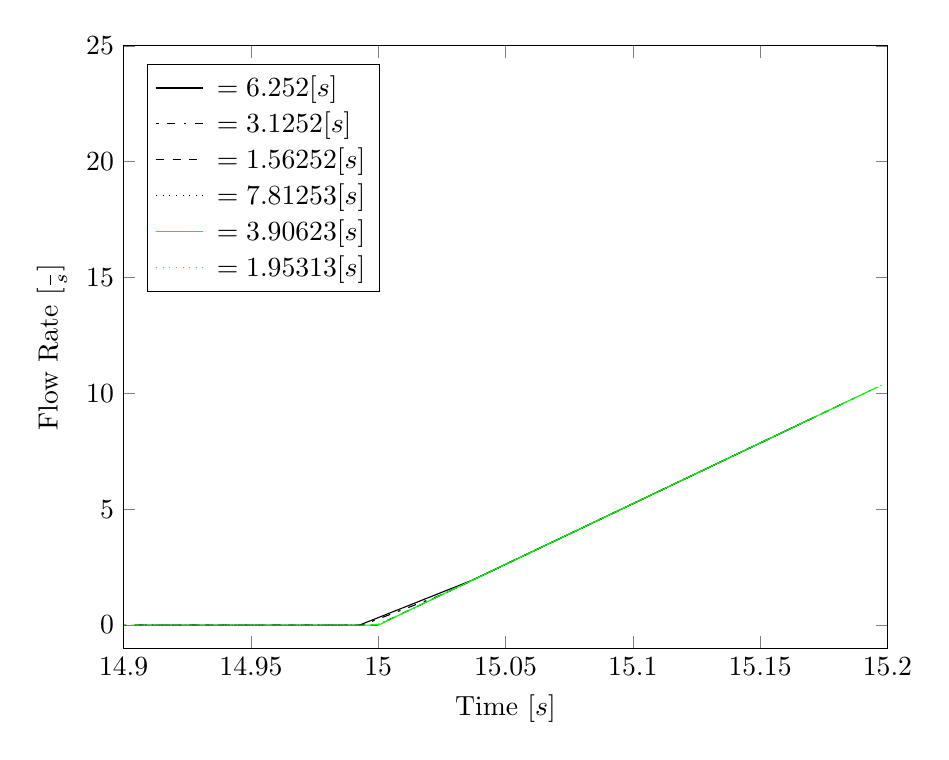
\begin{tikzpicture}

\begin{axis}[%
width=0.8\textwidth,
height=0.630967741935484\textwidth,
scale only axis,
xmin=14.9,
xmax=15.2,
xlabel={Time $[\text{s}]$},
ymin=-1,
ymax=25,
ylabel={Flow Rate $[ \frac{\lbm{}}{\text{s}} ]$},
legend style={at={(0.03,0.97)},anchor=north west,draw=black,fill=white,legend cell align=left}
]
\addplot [
color=black,
solid
]
table[row sep=crcr]{
14.9042348861694 0\\
14.9484453201294 0\\
14.9926567077637 0\\
15.0368671417236 1.93454301357269\\
15.0810785293579 4.24624395370483\\
15.1252889633179 6.56158781051636\\
15.1694993972778 8.87692451477051\\
};
\addlegendentry{$\dtmax{} = \expneg{6.25}{2}{[s]}$};

\addplot [
color=black,
dash pattern=on 1pt off 3pt on 3pt off 3pt
]
table[row sep=crcr]{
14.9000101089478 0\\
14.9312601089478 0\\
14.9625101089478 0\\
14.9937601089478 0\\
15.0250101089478 1.31288325786591\\
15.0562601089478 2.94648385047913\\
15.0875101089478 4.58305835723877\\
15.1187601089478 6.21962881088257\\
15.1500101089478 7.8562273979187\\
15.1812601089478 9.49282932281494\\
};
\addlegendentry{$\dtmax{} = \expneg{3.125}{2}{[s]}$};

\addplot [
color=black,
dashed
]
table[row sep=crcr]{
14.9059162139893 0\\
14.9215412139893 0\\
14.9371662139893 0\\
14.9527912139893 0\\
14.9684162139893 0\\
14.9840412139893 0\\
14.9996662139893 0\\
15.0152912139893 0.801035642623901\\
15.0309162139893 1.61912643909454\\
15.0465412139893 2.43743634223938\\
15.0621662139893 3.25572896003723\\
15.0777912139893 4.07402896881104\\
15.0934162139893 4.89233016967773\\
15.1090412139893 5.71063137054443\\
15.1246662139893 6.52893209457397\\
15.1402912139893 7.34723329544067\\
15.1559162139893 8.16562271118164\\
15.1715412139893 8.98390865325928\\
15.1871662139893 9.80219173431396\\
};
\addlegendentry{$\dtmax{} = \expneg{1.5625}{2}{[s]}$};

\addplot [
color=black,
dotted
]
table[row sep=crcr]{
14.905800819397 0\\
14.913613319397 0\\
14.921425819397 0\\
14.929238319397 0\\
14.937050819397 0\\
14.944863319397 0\\
14.952675819397 0\\
14.960488319397 0\\
14.968300819397 0\\
14.976113319397 0\\
14.983925819397 0\\
14.991738319397 0\\
14.999550819397 0\\
15.007363319397 0.385915666818619\\
15.015175819397 0.794798016548157\\
15.022988319397 1.2039543390274\\
15.030800819397 1.61310076713562\\
15.038613319397 2.02225089073181\\
15.046425819397 2.43140125274658\\
15.054238319397 2.84055185317993\\
15.062050819397 3.24970245361328\\
15.069863319397 3.65885305404663\\
15.077675819397 4.06804847717285\\
15.085488319397 4.47719144821167\\
15.093300819397 4.88633298873901\\
15.101113319397 5.29547691345215\\
15.108925819397 5.70462226867676\\
15.116738319397 6.11376953125\\
15.124550819397 6.5229172706604\\
15.132363319397 6.93206596374512\\
15.140175819397 7.34121513366699\\
15.147988319397 7.75036430358887\\
15.155800819397 8.15951347351074\\
15.163613319397 8.56866359710693\\
15.171425819397 8.97781372070313\\
15.179238319397 9.38696384429932\\
15.187050819397 9.79611396789551\\
15.194863319397 10.2052640914917\\
};
\addlegendentry{$\dtmax{} = \expneg{7.8125}{3}{[s]}$};

\addplot [
color=green,
solid
]
table[row sep=crcr]{
14.9033002853394 0\\
14.9072065353394 0\\
14.9111127853394 0\\
14.9150190353394 0\\
14.9189252853394 0\\
14.9228315353394 0\\
14.9267377853394 0\\
14.9306440353394 0\\
14.9345502853394 0\\
14.9384565353394 0\\
14.9423627853394 0\\
14.946268081665 0\\
14.950174331665 0\\
14.954080581665 0\\
14.957986831665 0\\
14.961893081665 0\\
14.965799331665 0\\
14.969705581665 0\\
14.973611831665 0\\
14.977518081665 0\\
14.981424331665 0\\
14.985330581665 0\\
14.989236831665 0\\
14.993143081665 0\\
14.997049331665 0\\
15.000955581665 0.0385664850473404\\
15.004861831665 0.254443943500519\\
15.008768081665 0.459155857563019\\
15.012674331665 0.66375058889389\\
15.016580581665 0.868322134017944\\
15.0204858779907 1.07289445400238\\
15.0243921279907 1.27746713161469\\
15.0282983779907 1.48203980922699\\
15.0322046279907 1.68661248683929\\
15.0361108779907 1.8911851644516\\
15.0400171279907 2.09577798843384\\
15.0439233779907 2.30034732818604\\
15.0478296279907 2.50491619110107\\
15.0517358779907 2.70948576927185\\
15.0556421279907 2.91405630111694\\
15.0595483779907 3.11862730979919\\
15.0634546279907 3.3231987953186\\
15.0673608779907 3.52777051925659\\
15.0712671279907 3.73234248161316\\
15.0751733779907 3.93691468238831\\
15.0790796279907 4.14148712158203\\
15.0829858779907 4.34605932235718\\
15.0868921279907 4.55063152313232\\
15.0907983779907 4.75520420074463\\
15.0947036743164 4.95977640151978\\
15.0986099243164 5.16434907913208\\
15.1025161743164 5.36892175674438\\
15.1064224243164 5.57349395751953\\
15.1103286743164 5.77806663513184\\
15.1142349243164 5.98263931274414\\
15.1181411743164 6.18721199035645\\
15.1220474243164 6.39178466796875\\
15.1259536743164 6.5963568687439\\
15.1298599243164 6.8009295463562\\
15.1337661743164 7.00550222396851\\
15.1376724243164 7.21007490158081\\
15.1415786743164 7.41464757919312\\
15.1454849243164 7.61922025680542\\
15.1493911743164 7.82379293441772\\
15.1532974243164 8.02836513519287\\
15.1572036743164 8.23293781280518\\
15.1611099243164 8.43751049041748\\
15.1650161743164 8.64208316802979\\
15.1689214706421 8.84665584564209\\
15.1728277206421 9.05122852325439\\
15.1767339706421 9.2558012008667\\
15.1806402206421 9.460373878479\\
15.1845464706421 9.66494655609131\\
15.1884527206421 9.86951923370361\\
15.1923589706421 10.0740909576416\\
15.1962652206421 10.2786636352539\\
};
\addlegendentry{$\dtmax{} = \expneg{3.9062}{3}{[s]}$};

\addplot [
color=green,
dotted
]
table[row sep=crcr]{
14.900221824646 0\\
14.902174949646 0\\
14.904128074646 0\\
14.906081199646 0\\
14.908034324646 0\\
14.909987449646 0\\
14.911940574646 0\\
14.913893699646 0\\
14.915846824646 0\\
14.9177989959717 0\\
14.9197521209717 0\\
14.9217052459717 0\\
14.9236583709717 0\\
14.9256114959717 0\\
14.9275646209717 0\\
14.9295177459717 0\\
14.9314708709717 0\\
14.9334239959717 0\\
14.9353771209717 0\\
14.9373302459717 0\\
14.9392833709717 0\\
14.9412364959717 0\\
14.9431896209717 0\\
14.9451427459717 0\\
14.9470958709717 0\\
14.9490489959717 0\\
14.9510021209717 0\\
14.9529552459717 0\\
14.9549083709717 0\\
14.9568614959717 0\\
14.9588146209717 0\\
14.9607677459717 0\\
14.9627208709717 0\\
14.9646739959717 0\\
14.9666271209717 0\\
14.9685802459717 0\\
14.9705333709717 0\\
14.9724864959717 0\\
14.9744396209717 0\\
14.9763927459717 0\\
14.9783458709717 0\\
14.9802989959717 0\\
14.9822521209717 0\\
14.9842052459717 0\\
14.9861583709717 0\\
14.9881114959717 0\\
14.9900646209717 0\\
14.9920167922974 0\\
14.9939699172974 0\\
14.9959230422974 0\\
14.9978761672974 0\\
14.9998292922974 0\\
15.0017824172974 0.0934739857912064\\
15.0037355422974 0.195629969239235\\
15.0056886672974 0.297931283712387\\
15.0076417922974 0.400224566459656\\
15.0095949172974 0.502510845661163\\
15.0115480422974 0.604796946048737\\
15.0135011672974 0.707083284854889\\
15.0154542922974 0.809369623661041\\
15.0174074172974 0.911655962467194\\
15.0193605422974 1.01394236087799\\
15.0213136672974 1.11622869968414\\
15.0232667922974 1.2185150384903\\
15.0252199172974 1.32080137729645\\
15.0271730422974 1.4230877161026\\
15.0291261672974 1.52537405490875\\
15.0310792922974 1.6276603937149\\
15.0330324172974 1.72994840145111\\
15.0349855422974 1.83223474025726\\
15.0369386672974 1.93452084064484\\
15.0388917922974 2.0368070602417\\
15.0408449172974 2.13909316062927\\
15.0427980422974 2.24137926101685\\
15.0447511672974 2.343665599823\\
15.0467042922974 2.44595170021057\\
15.0486574172974 2.54823803901672\\
15.0506105422974 2.65052437782288\\
15.0525636672974 2.75281047821045\\
15.0545167922974 2.8550968170166\\
15.0564699172974 2.95738315582275\\
15.0584230422974 3.05966949462891\\
15.0603761672974 3.16195583343506\\
15.0623292922974 3.26424217224121\\
15.0642824172974 3.36652827262878\\
15.066234588623 3.46881461143494\\
15.068187713623 3.57110095024109\\
15.070140838623 3.67338728904724\\
15.072093963623 3.77567362785339\\
15.074047088623 3.87795996665955\\
15.076000213623 3.9802463054657\\
15.077953338623 4.08253288269043\\
15.079906463623 4.18481874465942\\
15.081859588623 4.28710508346558\\
15.083812713623 4.38939142227173\\
15.085765838623 4.49167776107788\\
15.087718963623 4.59396409988403\\
15.089672088623 4.69625043869019\\
15.091625213623 4.79853677749634\\
15.093578338623 4.90082311630249\\
15.095531463623 5.00310945510864\\
15.097484588623 5.10539579391479\\
15.099437713623 5.20768213272095\\
15.101390838623 5.3099684715271\\
15.103343963623 5.41225481033325\\
15.105297088623 5.5145411491394\\
15.107250213623 5.61682748794556\\
15.109203338623 5.71911382675171\\
15.111156463623 5.82140016555786\\
15.113109588623 5.92368650436401\\
15.115062713623 6.02597284317017\\
15.117015838623 6.12825918197632\\
15.118968963623 6.23054552078247\\
15.120922088623 6.33283185958862\\
15.122875213623 6.43511819839478\\
15.124828338623 6.53740453720093\\
15.126781463623 6.63969087600708\\
15.128734588623 6.74197721481323\\
15.130687713623 6.84426355361938\\
15.132640838623 6.94654989242554\\
15.134593963623 7.04883623123169\\
15.136547088623 7.15112257003784\\
15.138500213623 7.25340890884399\\
15.1404523849487 7.35569524765015\\
15.1424055099487 7.4579815864563\\
15.1443586349487 7.56026792526245\\
15.1463117599487 7.6625542640686\\
15.1482648849487 7.76484060287476\\
15.1502180099487 7.86712646484375\\
15.1521711349487 7.9694128036499\\
15.1541242599487 8.07169914245605\\
15.1560773849487 8.17398548126221\\
15.1580305099487 8.27627182006836\\
15.1599836349487 8.37855815887451\\
15.1619367599487 8.48084449768066\\
15.1638898849487 8.58313083648682\\
15.1658430099487 8.68541717529297\\
15.1677961349487 8.78770351409912\\
15.1697492599487 8.88998985290527\\
15.1717023849487 8.99227619171143\\
15.1736555099487 9.09456253051758\\
15.1756086349487 9.19684886932373\\
15.1775617599487 9.29913520812988\\
15.1795148849487 9.40142154693604\\
15.1814680099487 9.50370788574219\\
15.1834211349487 9.60599422454834\\
15.1853742599487 9.70828056335449\\
15.1873273849487 9.81056690216064\\
15.1892805099487 9.9128532409668\\
15.1912336349487 10.0151395797729\\
15.1931867599487 10.1174259185791\\
15.1951398849487 10.2197122573853\\
15.1970930099487 10.3219976425171\\
15.1990461349487 10.4242839813232\\
};
\addlegendentry{$\dtmax{} = \expneg{1.9531}{3}{[s]}$};

\end{axis}
\end{tikzpicture}%
\caption{Zoom of flow rate in nonlinear solutions to the valve problem.}
\label{fig:valveNlnSols}
\end{figure}

These results indicate that the linear solver's timestep refinement serves the purpose of trying to resolve an isolated linearization error in a single channel of the problem.
By using the nonlinear solver, that error is removed and subsequent timestep reductions is not necessary to obtain the physical solution.
However, \tab{tab:valveNlnDataTable} shows that the nonlinear solver takes more cpu time per timestep than the linear solver.

\begin{table}[h!t]
\centering
\singlespace
\pgfplotstabletypeset[sci zerofill,sci E, col sep=comma,
	columns/0/.style={ column name= $[ \text{s} ]$, precision=1},
	columns/1/.style={ column name= $[ - ]$, int detect},
	columns/2/.style={ column name= $[ \text{s} ]$, precision=3},
	columns/3/.style={ column name= $[ \text{s} ]$, precision=3},
	every head row/.style={
		before row={
			\toprule
			\dtmax{} & $N_{t}$ & $T_{\text{CPU}}$& $\frac{T_{\text{CPU}}}{N_{t}}$ \\
		},
		after row=\midrule
	},
	every last row/.style={
after row=\bottomrule}]{tables/valveNlnData.tex}

\caption{Rum time data for the valve problem using the nonlinear solver.}
\label{tab:valveNlnDataTable}
\end{table}

Given that the nonlinearities in this problem are clearly isolated in a single channel, using the domain decomposition algorithm provides a simple test to determine if a nonlinearly converged solution can be obtained at a lower computational cost than the full nonlinear solver.
The use of the domain decomposition algorithm in this problem is restricted to the channel with the valve.
The other three channels are not included in the nonlinear domain.
The same set of timesteps is run to collect data.
\fig{fig:valveDom6pt25em02} shows the solution as obtained with \dtmax{} = \expneg{6.25}{2}{[s]}.
The results in this figure are qualitatively indistinguishable from the results of the nonlinear solver.

\begin{figure}[h!t]
\centering
% This file was created by matlab2tikz v0.4.3.
% Copyright (c) 2008--2013, Nico Schlömer <nico.schloemer@gmail.com>
% All rights reserved.
% 
\tikzsetnextfilename{plots/valveDom6pt2500em02_pdf}
\begin{tikzpicture}

\begin{axis}[%
width=\mytikzpicwidth,
height=\mytikzpicheight,
scale only axis,
xmin=0,
xmax=20,
xlabel={Time $[\text{s}]$},
ymin=-5,
ymax=125,
ylabel={Flow Rate $[ \frac{\lbm{}}{\text{s}} ]$},
legend style={draw=black,fill=white,legend cell align=left}
]
\addplot [
color=black,
solid
]
table[row sep=crcr]{
0 0\\
9.99999974737875e-06 -2.68723052698761e-08\\
2.49999993684469e-05 5.97379596456449e-07\\
4.75000015285332e-05 1.5992671251297e-05\\
8.12500002211891e-05 0.000229224911890924\\
0.000131875000079162 0.00192544842138886\\
0.000207812496228144 0.00898910593241453\\
0.000321718747727573 0.0234754215925932\\
0.000492578139528632 0.0383502058684826\\
0.00074886716902256 0.0502719767391682\\
0.00113330082967877 0.0704958811402321\\
0.00170995120424777 0.108530916273594\\
0.00257492670789361 0.167750313878059\\
0.00387239013798535 0.258952885866165\\
0.00529959984123707 0.363639861345291\\
0.00686953077092767 0.484229981899261\\
0.0085964547470212 0.623396694660187\\
0.0104960706084967 0.784338176250458\\
0.0125856483355165 0.970849931240082\\
0.014884184114635 1.18742954730988\\
0.0174125730991364 1.43940579891205\\
0.020193800330162 1.73308956623077\\
0.0232531521469355 2.07594513893127\\
0.0266184378415346 2.4767849445343\\
0.0303202513605356 2.94598364830017\\
0.0343922488391399 3.49570560455322\\
0.0388714447617531 4.14013338088989\\
0.0437985584139824 4.89567756652832\\
0.0492183864116669 5.78112745285034\\
0.0551801957190037 6.81768989562988\\
0.0617381855845451 8.02883529663086\\
0.0689519718289375 9.43983745574951\\
0.0768871381878853 11.0768632888794\\
0.0856158286333084 12.9654607772827\\
0.095217376947403 15.1283092498779\\
0.105779089033604 17.5821762084961\\
0.117396965622902 20.3342571258545\\
0.13017663359642 23.3783740997314\\
0.144234269857407 26.6919059753418\\
0.159697666764259 30.2346706390381\\
0.176707401871681 33.9509391784668\\
0.195418119430542 37.7751693725586\\
0.215999901294708 41.6409111022949\\
0.238639861345291 45.4909553527832\\
0.2635438144207 49.2860527038574\\
0.290938168764114 53.0097274780273\\
0.321071952581406 56.6680793762207\\
0.354219108819962 60.2851753234863\\
0.390680998563766 63.8959426879883\\
0.427134186029434 67.2247619628906\\
0.461836785078049 70.1926651000977\\
0.495115727186203 72.8892974853516\\
0.527189493179321 75.372917175293\\
0.558222532272339 77.6839752197266\\
0.588342726230621 79.8516006469727\\
0.617652356624603 81.8974990844727\\
0.646234631538391 83.8383636474609\\
0.674158751964569 85.6873397827148\\
0.701483011245728 87.4550094604492\\
0.728256940841675 89.1500778198242\\
0.754523456096649 90.77978515625\\
0.780319631099701 92.3502655029297\\
0.805678188800812 93.8667373657227\\
0.830627858638763 95.3337249755859\\
0.855194389820099 96.7551498413086\\
0.879400551319122 98.1344680786133\\
0.903267025947571 99.4747085571289\\
0.926812350749969 100.778564453125\\
0.950053453445435 102.048461914063\\
0.973005652427673 103.286552429199\\
0.995683073997498 104.494781494141\\
1.01809847354889 105.217460632324\\
1.0402637720108 105.585472106934\\
1.06237816810608 105.774543762207\\
1.08448839187622 105.871826171875\\
1.10659623146057 105.921867370605\\
1.12870299816132 105.947608947754\\
1.15080916881561 105.960845947266\\
1.17291498184204 105.967651367188\\
1.19502067565918 105.971153259277\\
1.21712636947632 105.972946166992\\
1.23923194408417 105.973876953125\\
1.26133751869202 105.974349975586\\
1.28344309329987 105.974594116211\\
1.30554866790771 105.974716186523\\
1.32765424251556 105.974784851074\\
1.34975969791412 105.974815368652\\
1.37186527252197 105.974830627441\\
1.39397084712982 105.974838256836\\
1.41607642173767 105.97484588623\\
1.43818199634552 105.97484588623\\
1.46028745174408 105.974853515625\\
1.48239302635193 105.974853515625\\
1.50449860095978 105.974853515625\\
1.52660417556763 105.974853515625\\
1.54870975017548 105.974853515625\\
1.57081520557404 105.974853515625\\
1.59292078018188 105.974853515625\\
1.61502635478973 105.974853515625\\
1.63713192939758 105.974853515625\\
1.65923750400543 105.974853515625\\
1.68134295940399 105.974853515625\\
1.70344853401184 105.974853515625\\
1.72555410861969 105.974853515625\\
1.74765968322754 105.974853515625\\
1.76976525783539 105.974853515625\\
1.79187071323395 105.974853515625\\
1.8139762878418 105.974853515625\\
1.83608186244965 105.974853515625\\
1.8581874370575 105.974853515625\\
1.88029301166534 105.974853515625\\
1.9023984670639 105.974853515625\\
1.92450404167175 105.974853515625\\
1.9466096162796 105.974853515625\\
1.96871519088745 105.974853515625\\
1.9908207654953 105.974853515625\\
2.01292634010315 105.974853515625\\
2.03503179550171 105.974853515625\\
2.05713748931885 105.974853515625\\
2.07924294471741 105.974853515625\\
2.10134840011597 105.974853515625\\
2.12345409393311 105.974853515625\\
2.14555954933167 105.974853515625\\
2.1676652431488 105.974853515625\\
2.18977069854736 105.974853515625\\
2.21187615394592 105.974853515625\\
2.23398184776306 105.974853515625\\
2.25608730316162 105.974853515625\\
2.27819299697876 105.974853515625\\
2.30029845237732 105.974853515625\\
2.32240390777588 105.974853515625\\
2.34450960159302 105.974853515625\\
2.36661505699158 105.974853515625\\
2.38872075080872 105.974853515625\\
2.41082620620728 105.974853515625\\
2.43293166160584 105.974853515625\\
2.45503735542297 105.974853515625\\
2.47714281082153 105.974853515625\\
2.49924850463867 105.974853515625\\
2.52135396003723 105.974853515625\\
2.54345941543579 105.974853515625\\
2.56556510925293 105.974853515625\\
2.58767056465149 105.974853515625\\
2.60977625846863 105.974853515625\\
2.63188171386719 105.974853515625\\
2.65398716926575 105.974853515625\\
2.67609286308289 105.974853515625\\
2.69819831848145 105.974853515625\\
2.72030401229858 105.974853515625\\
2.74240946769714 105.974853515625\\
2.7645149230957 105.974853515625\\
2.78662061691284 105.974853515625\\
2.8087260723114 105.974853515625\\
2.83083176612854 105.974853515625\\
2.8529372215271 105.974853515625\\
2.87504267692566 105.974853515625\\
2.8971483707428 105.974853515625\\
2.91925382614136 105.974853515625\\
2.9413595199585 105.974853515625\\
2.96346497535706 105.974853515625\\
2.98557043075562 105.974853515625\\
3.00767612457275 105.776901245117\\
3.02978157997131 105.100280761719\\
3.0519700050354 104.171333312988\\
3.07440447807312 103.101539611816\\
3.09709739685059 101.951995849609\\
3.12005996704102 100.754364013672\\
3.14330291748047 99.5247421264648\\
3.166836977005 98.2710571289063\\
3.19067335128784 96.9970092773438\\
3.21482396125793 95.7041015625\\
3.2393012046814 94.392707824707\\
3.26411890983582 93.0626068115234\\
3.28929138183594 91.7132720947266\\
3.31483387947083 90.3440017700195\\
3.34076333045959 88.9539413452148\\
3.36709761619568 87.5421447753906\\
3.39385652542114 86.1075820922852\\
3.42106103897095 84.6491241455078\\
3.44873404502869 83.1655502319336\\
3.47690057754517 81.6555328369141\\
3.50558733940125 80.1175994873047\\
3.53482460975647 78.550163269043\\
3.5646448135376 76.9514694213867\\
3.59508395195007 75.3195953369141\\
3.62618231773376 73.6523895263672\\
3.65798377990723 71.9474716186523\\
3.69053816795349 70.2022018432617\\
3.72390079498291 68.4135818481445\\
3.75813484191895 66.5782623291016\\
3.79331135749817 64.6924133300781\\
3.82951164245605 62.7516708374023\\
3.86682963371277 60.7510070800781\\
3.90537428855896 58.6845817565918\\
3.94527339935303 56.5455436706543\\
3.98667812347412 54.3257865905762\\
4.02976989746094 53.2729530334473\\
4.07350301742554 53.0479316711426\\
4.11750602722168 53.0003852844238\\
4.16167545318604 52.9903907775879\\
4.2058801651001 52.9882926940918\\
4.2500901222229 52.9878540039063\\
4.29430055618286 52.9877624511719\\
4.33851099014282 52.9877433776855\\
4.38272142410278 52.9877395629883\\
4.4269323348999 52.9877395629883\\
4.47114324569702 52.9877395629883\\
4.51535367965698 52.9877395629883\\
4.5595645904541 52.9877395629883\\
4.60377550125122 52.9877395629883\\
4.64798641204834 52.9877395629883\\
4.69219732284546 52.9877395629883\\
4.73640823364258 52.9877395629883\\
4.7806191444397 52.9877395629883\\
4.82482957839966 52.9877395629883\\
4.86904048919678 52.9877395629883\\
4.9132513999939 52.9877395629883\\
4.95746231079102 52.9877395629883\\
5.00167322158813 52.9877395629883\\
5.04588413238525 52.9877395629883\\
5.09009504318237 52.9877395629883\\
5.13430547714233 52.9877395629883\\
5.17851638793945 52.9877395629883\\
5.22272729873657 52.9877395629883\\
5.26693820953369 52.9877395629883\\
5.31114912033081 52.9877395629883\\
5.35536003112793 52.9877395629883\\
5.39957046508789 52.9877395629883\\
5.44378137588501 52.9877395629883\\
5.48799228668213 52.9877395629883\\
5.53220319747925 52.9877395629883\\
5.57641410827637 52.9877395629883\\
5.62062501907349 52.9877395629883\\
5.66483592987061 52.9877395629883\\
5.70904636383057 52.9877395629883\\
5.75325727462769 52.9877395629883\\
5.7974681854248 52.9877395629883\\
5.84167909622192 52.9877395629883\\
5.88589000701904 52.9877395629883\\
5.93010091781616 52.9877395629883\\
5.97431182861328 52.9877395629883\\
6.01852226257324 52.9877395629883\\
6.06273317337036 52.9877395629883\\
6.10694408416748 52.9877395629883\\
6.1511549949646 52.9877395629883\\
6.19536590576172 52.9877395629883\\
6.23957681655884 52.9877395629883\\
6.28378772735596 52.9877395629883\\
6.32799816131592 52.9877395629883\\
6.37220907211304 52.9877395629883\\
6.41641998291016 52.9877395629883\\
6.46063089370728 52.9877395629883\\
6.50484180450439 52.9877395629883\\
6.54905271530151 52.9877395629883\\
6.59326362609863 52.9877395629883\\
6.63747406005859 52.9877395629883\\
6.68168497085571 52.9877395629883\\
6.72589588165283 52.9877395629883\\
6.77010679244995 52.9877395629883\\
6.81431770324707 52.9877395629883\\
6.85852861404419 52.9877395629883\\
6.90273904800415 52.9877395629883\\
6.94694995880127 52.9877395629883\\
6.99116086959839 52.9877395629883\\
7.03537178039551 52.2437324523926\\
7.07958269119263 51.1552505493164\\
7.12379360198975 49.995246887207\\
7.16800451278687 48.8206787109375\\
7.21221494674683 47.643196105957\\
7.25642585754395 46.465145111084\\
7.30063676834106 45.286979675293\\
7.34484767913818 44.1087989807129\\
7.3890585899353 42.9306106567383\\
7.43326950073242 41.7524223327637\\
7.47748041152954 40.5742340087891\\
7.5216908454895 39.3960456848145\\
7.56590175628662 38.2178535461426\\
7.61011266708374 37.039665222168\\
7.65432357788086 35.8614768981934\\
7.69853448867798 34.6832847595215\\
7.7427453994751 33.5050964355469\\
7.78695631027222 32.326904296875\\
7.83116674423218 31.1487159729004\\
7.8753776550293 29.9705238342285\\
7.91958856582642 28.7923336029053\\
7.96379947662354 27.614143371582\\
8.0080099105835 26.624584197998\\
8.05222129821777 26.509183883667\\
8.09643173217773 26.4956932067871\\
8.14064311981201 26.4941177368164\\
8.18485355377197 26.4939346313477\\
8.22906494140625 26.4939117431641\\
8.27327537536621 26.4939098358154\\
8.31748580932617 26.4939098358154\\
8.36169719696045 26.4939079284668\\
8.40590763092041 26.4939079284668\\
8.45011901855469 26.4939079284668\\
8.49432945251465 26.4939079284668\\
8.53854084014893 26.4939079284668\\
8.58275127410889 26.4939079284668\\
8.62696170806885 26.4939079284668\\
8.67117309570313 26.4939079284668\\
8.71538352966309 26.4939079284668\\
8.75959491729736 26.4939079284668\\
8.80380535125732 26.4939079284668\\
8.8480167388916 26.4939079284668\\
8.89222717285156 26.4939079284668\\
8.93643760681152 26.4939079284668\\
8.9806489944458 26.4939079284668\\
9.02485942840576 26.4939079284668\\
9.06907081604004 26.4939079284668\\
9.11328125 26.4939079284668\\
9.15749263763428 26.4939079284668\\
9.20170307159424 26.4939079284668\\
9.2459135055542 26.4939079284668\\
9.29012489318848 26.4939079284668\\
9.33433532714844 26.4939079284668\\
9.37854671478271 26.4939079284668\\
9.42275714874268 26.4939079284668\\
9.46696758270264 26.4939079284668\\
9.51117897033691 26.4939079284668\\
9.55538940429688 26.4939079284668\\
9.59960079193115 26.4939079284668\\
9.64381122589111 26.4939079284668\\
9.68802261352539 26.4939079284668\\
9.73223304748535 26.4939079284668\\
9.77644348144531 26.4939079284668\\
9.82065486907959 26.4939079284668\\
9.86486530303955 26.4939079284668\\
9.90907669067383 26.4939079284668\\
9.95328712463379 26.4939079284668\\
9.99749851226807 26.4939079284668\\
10.041708946228 26.4939079284668\\
10.085919380188 26.4939079284668\\
10.1301307678223 26.4939079284668\\
10.1743412017822 26.4939079284668\\
10.2185525894165 26.4939079284668\\
10.2627630233765 26.4939079284668\\
10.3069744110107 26.4939079284668\\
10.3511848449707 26.4939079284668\\
10.3953952789307 26.4939079284668\\
10.4396066665649 26.4939079284668\\
10.4838171005249 26.4939079284668\\
10.5280284881592 26.4939079284668\\
10.5722389221191 26.4939079284668\\
10.6164503097534 26.4939079284668\\
10.6606607437134 26.4939079284668\\
10.7048711776733 26.4939079284668\\
10.7490825653076 26.4939079284668\\
10.7932929992676 26.4939079284668\\
10.8375043869019 26.4939079284668\\
10.8817148208618 26.4939079284668\\
10.9259262084961 26.4939079284668\\
10.9701366424561 26.4939079284668\\
11.014347076416 26.1576251983643\\
11.0585584640503 25.0768013000488\\
11.1027688980103 23.90940284729\\
11.1469802856445 22.7323703765869\\
11.1911907196045 21.5542984008789\\
11.2354021072388 20.3761196136475\\
11.2796125411987 19.1979331970215\\
11.3238229751587 18.0197467803955\\
11.368034362793 16.8415603637695\\
11.4122447967529 15.6633768081665\\
11.4561223983765 14.4940776824951\\
11.5 13.3247852325439\\
11.54421043396 12.1466178894043\\
11.5884218215942 10.9683303833008\\
11.6326322555542 9.79013252258301\\
11.6768436431885 8.61193943023682\\
11.7210540771484 7.43374538421631\\
11.7652654647827 6.25555229187012\\
11.8094758987427 5.07735872268677\\
11.8536863327026 3.89916563034058\\
11.8978977203369 2.72097659111023\\
11.9421081542969 1.54277789592743\\
11.9863195419312 0.36458432674408\\
12.0305299758911 0\\
12.0747413635254 0\\
12.1189517974854 0\\
12.1631622314453 0\\
12.2073736190796 0\\
12.2515840530396 0\\
12.2957954406738 0\\
12.3400058746338 0\\
12.3842172622681 0\\
12.428427696228 0\\
12.472638130188 0\\
12.5168495178223 0\\
12.5610599517822 0\\
12.6052713394165 0\\
12.6494817733765 0\\
12.6936931610107 0\\
12.7379035949707 0\\
12.7821140289307 0\\
12.8263254165649 0\\
12.8705358505249 0\\
12.9147472381592 0\\
12.9589576721191 0\\
13.0031690597534 0\\
13.0473794937134 0\\
13.0915899276733 0\\
13.1358013153076 0\\
13.1800117492676 0\\
13.2242231369019 0\\
13.2684335708618 0\\
13.3126440048218 0\\
13.3568553924561 0\\
13.401065826416 0\\
13.4452772140503 0\\
13.4894876480103 0\\
13.5336990356445 0\\
13.5779094696045 0\\
13.6221199035645 0\\
13.6663312911987 0\\
13.7105417251587 0\\
13.754753112793 0\\
13.7989635467529 0\\
13.8431749343872 0\\
13.8873853683472 0\\
13.9315958023071 0\\
13.9758071899414 0\\
14.0200176239014 0\\
14.0642290115356 0\\
14.1084394454956 0\\
14.1526508331299 0\\
14.1968612670898 0\\
14.2410717010498 0\\
14.2852830886841 0\\
14.329493522644 0\\
14.3737049102783 0\\
14.4179153442383 0\\
14.4621267318726 0\\
14.5063371658325 0\\
14.5505475997925 0\\
14.5947589874268 0\\
14.6389694213867 0\\
14.683180809021 0\\
14.727391242981 0\\
14.7716026306152 0\\
14.8158130645752 0\\
14.8600234985352 0\\
14.9042348861694 0\\
14.9484453201294 0\\
14.9926567077637 0\\
15.0368671417236 1.93454313278198\\
15.0810785293579 4.24624395370483\\
15.1252889633179 6.56158828735352\\
15.1694993972778 8.87692451477051\\
15.2137107849121 11.1922979354858\\
15.2579212188721 13.5076742172241\\
15.3021326065063 15.8230504989624\\
15.3463430404663 18.138427734375\\
15.3905544281006 20.4538021087646\\
15.4347648620605 22.7691783905029\\
15.4789752960205 25.0845527648926\\
15.5231866836548 27.3999271392822\\
15.5673971176147 29.7153015136719\\
15.611608505249 32.0306739807129\\
15.655818939209 34.3460464477539\\
15.7000303268433 36.6614189147949\\
15.7442407608032 38.9767913818359\\
15.7884511947632 41.2921600341797\\
15.8326625823975 43.6075286865234\\
15.8768730163574 45.9228973388672\\
15.9210844039917 48.2382850646973\\
15.9652948379517 50.5536499023438\\
16.0095062255859 52.4762725830078\\
16.0537166595459 52.8805809020996\\
16.0967807769775 52.9648361206055\\
16.1407527923584 52.9829216003418\\
16.1849117279053 52.9867286682129\\
16.2291107177734 52.9875259399414\\
16.2733192443848 52.9876937866211\\
16.3175296783447 52.9877281188965\\
16.3617401123047 52.987735748291\\
16.4059524536133 52.9877395629883\\
16.4501628875732 52.9877395629883\\
16.4943733215332 52.9877395629883\\
16.5385837554932 52.9877395629883\\
16.5827941894531 52.9877395629883\\
16.6270065307617 52.9877395629883\\
16.6712169647217 52.9877395629883\\
16.7154273986816 52.9877395629883\\
16.7596378326416 52.9877395629883\\
16.8038482666016 52.9877395629883\\
16.8480606079102 52.9877395629883\\
16.8922710418701 52.9877395629883\\
16.9364814758301 52.9877395629883\\
16.98069190979 52.9877395629883\\
17.0249042510986 52.9877395629883\\
17.0691146850586 52.9877395629883\\
17.1133251190186 52.9877395629883\\
17.1575355529785 52.9877395629883\\
17.2017459869385 52.9877395629883\\
17.2459583282471 52.9877395629883\\
17.290168762207 52.9877395629883\\
17.334379196167 52.9877395629883\\
17.378589630127 52.9877395629883\\
17.4228000640869 52.9877395629883\\
17.4670124053955 52.9877395629883\\
17.5112228393555 52.9877395629883\\
17.5554332733154 52.9877395629883\\
17.5996437072754 52.9877395629883\\
17.643856048584 52.9877395629883\\
17.6880664825439 52.9877395629883\\
17.7322769165039 52.9877395629883\\
17.7764873504639 52.9877395629883\\
17.8206977844238 52.9877395629883\\
17.8649101257324 52.9877395629883\\
17.9091205596924 52.9877395629883\\
17.9533309936523 52.9877395629883\\
17.9975414276123 52.9877395629883\\
18.0417518615723 52.9877395629883\\
18.0859642028809 52.9877395629883\\
18.1301746368408 52.9877395629883\\
18.1743850708008 52.9877395629883\\
18.2185955047607 52.9877395629883\\
18.2628078460693 52.9877395629883\\
18.3070182800293 52.9877395629883\\
18.3512287139893 52.9877395629883\\
18.3954391479492 52.9877395629883\\
18.4396495819092 52.9877395629883\\
18.4838619232178 52.9877395629883\\
18.5280723571777 52.9877395629883\\
18.5722827911377 52.9877395629883\\
18.6164932250977 52.9877395629883\\
18.6607036590576 52.9877395629883\\
18.7049160003662 52.9877395629883\\
18.7491264343262 52.9877395629883\\
18.7933368682861 52.9877395629883\\
18.8375473022461 52.9877395629883\\
18.8817577362061 52.9877395629883\\
18.9259700775146 52.9877395629883\\
18.962984085083 52.9877395629883\\
19 52.9877395629883\\
};
\addlegendentry{$A_{r}(t)$};

\addplot [
color=black,
dash pattern=on 1pt off 3pt on 3pt off 3pt
]
table[row sep=crcr]{
0 0\\
9.99999974737875e-06 7.34263050361506e-09\\
2.49999993684469e-05 6.82787117511907e-07\\
4.75000015285332e-05 1.61537918756949e-05\\
8.12500002211891e-05 0.000229484256124124\\
0.000131875000079162 0.00192573899403214\\
0.000207812496228144 0.00898905657231808\\
0.000321718747727573 0.0234745796769857\\
0.000492578139528632 0.0383488200604916\\
0.00074886716902256 0.0502703413367271\\
0.00113330082967877 0.0704929903149605\\
0.00170995120424777 0.108524538576603\\
0.00257492670789361 0.167731299996376\\
0.00387239013798535 0.258889704942703\\
0.00529959984123707 0.363474696874619\\
0.00686953077092767 0.483860403299332\\
0.0085964547470212 0.622648656368256\\
0.0104960706084967 0.782925307750702\\
0.0125856483355165 0.968311131000519\\
0.014884184114635 1.18303418159485\\
0.0174125730991364 1.43201053142548\\
0.020193800330162 1.72092187404633\\
0.0232531521469355 2.05627965927124\\
0.0266184378415346 2.44546175003052\\
0.0303202513605356 2.8966953754425\\
0.0343922488391399 3.41895937919617\\
0.0388714447617531 4.0217547416687\\
0.0437985584139824 4.71469640731812\\
0.0492183864116669 5.50687074661255\\
0.0551801957190037 6.40590953826904\\
0.0617381855845451 7.41679286956787\\
0.0689519718289375 8.54045581817627\\
0.0768871381878853 9.77241897583008\\
0.0856158286333084 11.1017980575562\\
0.095217376947403 12.5111665725708\\
0.105779089033604 13.9776849746704\\
0.117396965622902 15.4756441116333\\
0.13017663359642 16.9800872802734\\
0.144234269857407 18.4706878662109\\
0.159697666764259 19.9348068237305\\
0.176707401871681 21.3688697814941\\
0.195418119430542 22.7777843475342\\
0.215999901294708 24.1727924346924\\
0.238639861345291 25.5685958862305\\
0.2635438144207 26.9806213378906\\
0.290938168764114 28.4230575561523\\
0.321071952581406 29.907886505127\\
0.354219108819962 31.4447612762451\\
0.390680998563766 33.0414009094238\\
0.427134186029434 34.5529632568359\\
0.461836785078049 35.9256439208984\\
0.495115727186203 37.1908950805664\\
0.527189493179321 38.3686904907227\\
0.558222532272339 39.473316192627\\
0.588342726230621 40.515495300293\\
0.617652356624603 41.5035820007324\\
0.646234631538391 42.4442443847656\\
0.674158751964569 43.342903137207\\
0.701483011245728 44.2040367126465\\
0.728256940841675 45.0314025878906\\
0.754523456096649 45.8281784057617\\
0.780319631099701 46.5970878601074\\
0.805678188800812 47.3404846191406\\
0.830627858638763 48.0604095458984\\
0.855194389820099 48.7586631774902\\
0.879400551319122 49.436824798584\\
0.903267025947571 50.0962944030762\\
0.926812350749969 50.7383270263672\\
0.950053453445435 51.3640441894531\\
0.973005652427673 51.9744567871094\\
0.995683073997498 52.5704765319824\\
1.01809847354889 52.844913482666\\
1.0402637720108 52.9383926391602\\
1.06237816810608 52.9706420898438\\
1.08448839187622 52.9818077087402\\
1.10659623146057 52.9856758117676\\
1.12870299816132 52.9870223999023\\
1.15080916881561 52.9874877929688\\
1.17291498184204 52.9876518249512\\
1.19502067565918 52.9877090454102\\
1.21712636947632 52.9877319335938\\
1.23923194408417 52.9877395629883\\
1.26133751869202 52.9877395629883\\
1.28344309329987 52.9877433776855\\
1.30554866790771 52.9877433776855\\
1.32765424251556 52.9877395629883\\
1.34975969791412 52.9877395629883\\
1.37186527252197 52.9877395629883\\
1.39397084712982 52.9877395629883\\
1.41607642173767 52.9877395629883\\
1.43818199634552 52.9877395629883\\
1.46028745174408 52.9877395629883\\
1.48239302635193 52.9877395629883\\
1.50449860095978 52.9877395629883\\
1.52660417556763 52.9877395629883\\
1.54870975017548 52.9877395629883\\
1.57081520557404 52.9877395629883\\
1.59292078018188 52.9877395629883\\
1.61502635478973 52.9877395629883\\
1.63713192939758 52.9877395629883\\
1.65923750400543 52.9877395629883\\
1.68134295940399 52.9877395629883\\
1.70344853401184 52.9877395629883\\
1.72555410861969 52.9877395629883\\
1.74765968322754 52.9877395629883\\
1.76976525783539 52.9877395629883\\
1.79187071323395 52.9877395629883\\
1.8139762878418 52.9877395629883\\
1.83608186244965 52.9877395629883\\
1.8581874370575 52.9877395629883\\
1.88029301166534 52.9877395629883\\
1.9023984670639 52.9877395629883\\
1.92450404167175 52.9877395629883\\
1.9466096162796 52.9877395629883\\
1.96871519088745 52.9877395629883\\
1.9908207654953 52.9877395629883\\
2.01292634010315 52.9877395629883\\
2.03503179550171 52.9877395629883\\
2.05713748931885 52.9877395629883\\
2.07924294471741 52.9877395629883\\
2.10134840011597 52.9877395629883\\
2.12345409393311 52.9877395629883\\
2.14555954933167 52.9877395629883\\
2.1676652431488 52.9877395629883\\
2.18977069854736 52.9877395629883\\
2.21187615394592 52.9877395629883\\
2.23398184776306 52.9877395629883\\
2.25608730316162 52.9877395629883\\
2.27819299697876 52.9877395629883\\
2.30029845237732 52.9877395629883\\
2.32240390777588 52.9877395629883\\
2.34450960159302 52.9877395629883\\
2.36661505699158 52.9877395629883\\
2.38872075080872 52.9877395629883\\
2.41082620620728 52.9877395629883\\
2.43293166160584 52.9877395629883\\
2.45503735542297 52.9877395629883\\
2.47714281082153 52.9877395629883\\
2.49924850463867 52.9877395629883\\
2.52135396003723 52.9877395629883\\
2.54345941543579 52.9877395629883\\
2.56556510925293 52.9877395629883\\
2.58767056465149 52.9877395629883\\
2.60977625846863 52.9877395629883\\
2.63188171386719 52.9877395629883\\
2.65398716926575 52.9877395629883\\
2.67609286308289 52.9877395629883\\
2.69819831848145 52.9877395629883\\
2.72030401229858 52.9877395629883\\
2.74240946769714 52.9877395629883\\
2.7645149230957 52.9877395629883\\
2.78662061691284 52.9877395629883\\
2.8087260723114 52.9877395629883\\
2.83083176612854 52.9877395629883\\
2.8529372215271 52.9877395629883\\
2.87504267692566 52.9877395629883\\
2.8971483707428 52.9877395629883\\
2.91925382614136 52.9877395629883\\
2.9413595199585 52.9877395629883\\
2.96346497535706 52.9877395629883\\
2.98557043075562 52.9877395629883\\
3.00767612457275 52.9877395629883\\
3.02978157997131 52.9877395629883\\
3.0519700050354 52.9877395629883\\
3.07440447807312 52.9877395629883\\
3.09709739685059 52.9877395629883\\
3.12005996704102 52.9877395629883\\
3.14330291748047 52.9877395629883\\
3.166836977005 52.9877395629883\\
3.19067335128784 52.9877395629883\\
3.21482396125793 52.9877395629883\\
3.2393012046814 52.9877395629883\\
3.26411890983582 52.9877395629883\\
3.28929138183594 52.9877395629883\\
3.31483387947083 52.9877395629883\\
3.34076333045959 52.9877395629883\\
3.36709761619568 52.9877395629883\\
3.39385652542114 52.9877395629883\\
3.42106103897095 52.9877395629883\\
3.44873404502869 52.9877395629883\\
3.47690057754517 52.9877395629883\\
3.50558733940125 52.9877395629883\\
3.53482460975647 52.9877395629883\\
3.5646448135376 52.9877395629883\\
3.59508395195007 52.9877395629883\\
3.62618231773376 52.9877395629883\\
3.65798377990723 52.9877395629883\\
3.69053816795349 52.9877395629883\\
3.72390079498291 52.9877395629883\\
3.75813484191895 52.9877395629883\\
3.79331135749817 52.9877395629883\\
3.82951164245605 52.9877395629883\\
3.86682963371277 52.9877395629883\\
3.90537428855896 52.9877395629883\\
3.94527339935303 52.9877395629883\\
3.98667812347412 52.9877395629883\\
4.02976989746094 52.9877395629883\\
4.07350301742554 52.9877395629883\\
4.11750602722168 52.9877395629883\\
4.16167545318604 52.9877395629883\\
4.2058801651001 52.9877395629883\\
4.2500901222229 52.9877395629883\\
4.29430055618286 52.9877395629883\\
4.33851099014282 52.9877395629883\\
4.38272142410278 52.9877395629883\\
4.4269323348999 52.9877395629883\\
4.47114324569702 52.9877395629883\\
4.51535367965698 52.9877395629883\\
4.5595645904541 52.9877395629883\\
4.60377550125122 52.9877395629883\\
4.64798641204834 52.9877395629883\\
4.69219732284546 52.9877395629883\\
4.73640823364258 52.9877395629883\\
4.7806191444397 52.9877395629883\\
4.82482957839966 52.9877395629883\\
4.86904048919678 52.9877395629883\\
4.9132513999939 52.9877395629883\\
4.95746231079102 52.9877395629883\\
5.00167322158813 52.9877395629883\\
5.04588413238525 52.9877395629883\\
5.09009504318237 52.9877395629883\\
5.13430547714233 52.9877395629883\\
5.17851638793945 52.9877395629883\\
5.22272729873657 52.9877395629883\\
5.26693820953369 52.9877395629883\\
5.31114912033081 52.9877395629883\\
5.35536003112793 52.9877395629883\\
5.39957046508789 52.9877395629883\\
5.44378137588501 52.9877395629883\\
5.48799228668213 52.9877395629883\\
5.53220319747925 52.9877395629883\\
5.57641410827637 52.9877395629883\\
5.62062501907349 52.9877395629883\\
5.66483592987061 52.9877395629883\\
5.70904636383057 52.9877395629883\\
5.75325727462769 52.9877395629883\\
5.7974681854248 52.9877395629883\\
5.84167909622192 52.9877395629883\\
5.88589000701904 52.9877395629883\\
5.93010091781616 52.9877395629883\\
5.97431182861328 52.9877395629883\\
6.01852226257324 52.9877395629883\\
6.06273317337036 52.9877395629883\\
6.10694408416748 52.9877395629883\\
6.1511549949646 52.9877395629883\\
6.19536590576172 52.9877395629883\\
6.23957681655884 52.9877395629883\\
6.28378772735596 52.9877395629883\\
6.32799816131592 52.9877395629883\\
6.37220907211304 52.9877395629883\\
6.41641998291016 52.9877395629883\\
6.46063089370728 52.9877395629883\\
6.50484180450439 52.9877395629883\\
6.54905271530151 52.9877395629883\\
6.59326362609863 52.9877395629883\\
6.63747406005859 52.9877395629883\\
6.68168497085571 52.9877395629883\\
6.72589588165283 52.9877395629883\\
6.77010679244995 52.9877395629883\\
6.81431770324707 52.9877395629883\\
6.85852861404419 52.9877395629883\\
6.90273904800415 52.9877395629883\\
6.94694995880127 52.9877395629883\\
6.99116086959839 52.9877395629883\\
7.03537178039551 52.9877395629883\\
7.07958269119263 52.9877395629883\\
7.12379360198975 52.9877395629883\\
7.16800451278687 52.9877395629883\\
7.21221494674683 52.9877395629883\\
7.25642585754395 52.9877395629883\\
7.30063676834106 52.9877395629883\\
7.34484767913818 52.9877395629883\\
7.3890585899353 52.9877395629883\\
7.43326950073242 52.9877395629883\\
7.47748041152954 52.9877395629883\\
7.5216908454895 52.9877395629883\\
7.56590175628662 52.9877395629883\\
7.61011266708374 52.9877395629883\\
7.65432357788086 52.9877395629883\\
7.69853448867798 52.9877395629883\\
7.7427453994751 52.9877395629883\\
7.78695631027222 52.9877395629883\\
7.83116674423218 52.9877395629883\\
7.8753776550293 52.9877395629883\\
7.91958856582642 52.9877395629883\\
7.96379947662354 52.9877395629883\\
8.0080099105835 52.9877395629883\\
8.05222129821777 52.9877395629883\\
8.09643173217773 52.9877395629883\\
8.14064311981201 52.9877395629883\\
8.18485355377197 52.9877395629883\\
8.22906494140625 52.9877395629883\\
8.27327537536621 52.9877395629883\\
8.31748580932617 52.9877395629883\\
8.36169719696045 52.9877395629883\\
8.40590763092041 52.9877395629883\\
8.45011901855469 52.9877395629883\\
8.49432945251465 52.9877395629883\\
8.53854084014893 52.9877395629883\\
8.58275127410889 52.9877395629883\\
8.62696170806885 52.9877395629883\\
8.67117309570313 52.9877395629883\\
8.71538352966309 52.9877395629883\\
8.75959491729736 52.9877395629883\\
8.80380535125732 52.9877395629883\\
8.8480167388916 52.9877395629883\\
8.89222717285156 52.9877395629883\\
8.93643760681152 52.9877395629883\\
8.9806489944458 52.9877395629883\\
9.02485942840576 52.9877395629883\\
9.06907081604004 52.9877395629883\\
9.11328125 52.9877395629883\\
9.15749263763428 52.9877395629883\\
9.20170307159424 52.9877395629883\\
9.2459135055542 52.9877395629883\\
9.29012489318848 52.9877395629883\\
9.33433532714844 52.9877395629883\\
9.37854671478271 52.9877395629883\\
9.42275714874268 52.9877395629883\\
9.46696758270264 52.9877395629883\\
9.51117897033691 52.9877395629883\\
9.55538940429688 52.9877395629883\\
9.59960079193115 52.9877395629883\\
9.64381122589111 52.9877395629883\\
9.68802261352539 52.9877395629883\\
9.73223304748535 52.9877395629883\\
9.77644348144531 52.9877395629883\\
9.82065486907959 52.9877395629883\\
9.86486530303955 52.9877395629883\\
9.90907669067383 52.9877395629883\\
9.95328712463379 52.9877395629883\\
9.99749851226807 52.9877395629883\\
10.041708946228 52.9877395629883\\
10.085919380188 52.9877395629883\\
10.1301307678223 52.9877395629883\\
10.1743412017822 52.9877395629883\\
10.2185525894165 52.9877395629883\\
10.2627630233765 52.9877395629883\\
10.3069744110107 52.9877395629883\\
10.3511848449707 52.9877395629883\\
10.3953952789307 52.9877395629883\\
10.4396066665649 52.9877395629883\\
10.4838171005249 52.9877395629883\\
10.5280284881592 52.9877395629883\\
10.5722389221191 52.9877395629883\\
10.6164503097534 52.9877395629883\\
10.6606607437134 52.9877395629883\\
10.7048711776733 52.9877395629883\\
10.7490825653076 52.9877395629883\\
10.7932929992676 52.9877395629883\\
10.8375043869019 52.9877395629883\\
10.8817148208618 52.9877395629883\\
10.9259262084961 52.9877395629883\\
10.9701366424561 52.9877395629883\\
11.014347076416 52.9877395629883\\
11.0585584640503 52.9877395629883\\
11.1027688980103 52.9877395629883\\
11.1469802856445 52.9877395629883\\
11.1911907196045 52.9877395629883\\
11.2354021072388 52.9877395629883\\
11.2796125411987 52.9877395629883\\
11.3238229751587 52.9877395629883\\
11.368034362793 52.9877395629883\\
11.4122447967529 52.9877395629883\\
11.4561223983765 52.9877395629883\\
11.5 52.9877395629883\\
11.54421043396 52.9877395629883\\
11.5884218215942 52.9877395629883\\
11.6326322555542 52.9877395629883\\
11.6768436431885 52.9877395629883\\
11.7210540771484 52.9877395629883\\
11.7652654647827 52.9877395629883\\
11.8094758987427 52.9877395629883\\
11.8536863327026 52.9877395629883\\
11.8978977203369 52.9877395629883\\
11.9421081542969 52.9877395629883\\
11.9863195419312 52.9877395629883\\
12.0305299758911 52.9877395629883\\
12.0747413635254 52.9877395629883\\
12.1189517974854 52.9877395629883\\
12.1631622314453 52.9877395629883\\
12.2073736190796 52.9877395629883\\
12.2515840530396 52.9877395629883\\
12.2957954406738 52.9877395629883\\
12.3400058746338 52.9877395629883\\
12.3842172622681 52.9877395629883\\
12.428427696228 52.9877395629883\\
12.472638130188 52.9877395629883\\
12.5168495178223 52.9877395629883\\
12.5610599517822 52.9877395629883\\
12.6052713394165 52.9877395629883\\
12.6494817733765 52.9877395629883\\
12.6936931610107 52.9877395629883\\
12.7379035949707 52.9877395629883\\
12.7821140289307 52.9877395629883\\
12.8263254165649 52.9877395629883\\
12.8705358505249 52.9877395629883\\
12.9147472381592 52.9877395629883\\
12.9589576721191 52.9877395629883\\
13.0031690597534 52.9877395629883\\
13.0473794937134 52.9877395629883\\
13.0915899276733 52.9877395629883\\
13.1358013153076 52.9877395629883\\
13.1800117492676 52.9877395629883\\
13.2242231369019 52.9877395629883\\
13.2684335708618 52.9877395629883\\
13.3126440048218 52.9877395629883\\
13.3568553924561 52.9877395629883\\
13.401065826416 52.9877395629883\\
13.4452772140503 52.9877395629883\\
13.4894876480103 52.9877395629883\\
13.5336990356445 52.9877395629883\\
13.5779094696045 52.9877395629883\\
13.6221199035645 52.9877395629883\\
13.6663312911987 52.9877395629883\\
13.7105417251587 52.9877395629883\\
13.754753112793 52.9877395629883\\
13.7989635467529 52.9877395629883\\
13.8431749343872 52.9877395629883\\
13.8873853683472 52.9877395629883\\
13.9315958023071 52.9877395629883\\
13.9758071899414 52.9877395629883\\
14.0200176239014 52.9877395629883\\
14.0642290115356 52.9877395629883\\
14.1084394454956 52.9877395629883\\
14.1526508331299 52.9877395629883\\
14.1968612670898 52.9877395629883\\
14.2410717010498 52.9877395629883\\
14.2852830886841 52.9877395629883\\
14.329493522644 52.9877395629883\\
14.3737049102783 52.9877395629883\\
14.4179153442383 52.9877395629883\\
14.4621267318726 52.9877395629883\\
14.5063371658325 52.9877395629883\\
14.5505475997925 52.9877395629883\\
14.5947589874268 52.9877395629883\\
14.6389694213867 52.9877395629883\\
14.683180809021 52.9877395629883\\
14.727391242981 52.9877395629883\\
14.7716026306152 52.9877395629883\\
14.8158130645752 52.9877395629883\\
14.8600234985352 52.9877395629883\\
14.9042348861694 52.9877395629883\\
14.9484453201294 52.9877395629883\\
14.9926567077637 52.9877395629883\\
15.0368671417236 52.9877395629883\\
15.0810785293579 52.9877395629883\\
15.1252889633179 52.9877395629883\\
15.1694993972778 52.9877395629883\\
15.2137107849121 52.9877395629883\\
15.2579212188721 52.9877395629883\\
15.3021326065063 52.9877395629883\\
15.3463430404663 52.9877395629883\\
15.3905544281006 52.9877395629883\\
15.4347648620605 52.9877395629883\\
15.4789752960205 52.9877395629883\\
15.5231866836548 52.9877395629883\\
15.5673971176147 52.9877395629883\\
15.611608505249 52.9877395629883\\
15.655818939209 52.9877395629883\\
15.7000303268433 52.9877395629883\\
15.7442407608032 52.9877395629883\\
15.7884511947632 52.9877395629883\\
15.8326625823975 52.9877395629883\\
15.8768730163574 52.9877395629883\\
15.9210844039917 52.9877395629883\\
15.9652948379517 52.9877395629883\\
16.0095062255859 52.9877395629883\\
16.0537166595459 52.9877395629883\\
16.0967807769775 52.9877395629883\\
16.1407527923584 52.9877395629883\\
16.1849117279053 52.9877395629883\\
16.2291107177734 52.9877395629883\\
16.2733192443848 52.9877395629883\\
16.3175296783447 52.9877395629883\\
16.3617401123047 52.9877395629883\\
16.4059524536133 52.9877395629883\\
16.4501628875732 52.9877395629883\\
16.4943733215332 52.9877395629883\\
16.5385837554932 52.9877395629883\\
16.5827941894531 52.9877395629883\\
16.6270065307617 52.9877395629883\\
16.6712169647217 52.9877395629883\\
16.7154273986816 52.9877395629883\\
16.7596378326416 52.9877395629883\\
16.8038482666016 52.9877395629883\\
16.8480606079102 52.9877395629883\\
16.8922710418701 52.9877395629883\\
16.9364814758301 52.9877395629883\\
16.98069190979 52.9877395629883\\
17.0249042510986 52.9877395629883\\
17.0691146850586 52.9877395629883\\
17.1133251190186 52.9877395629883\\
17.1575355529785 52.9877395629883\\
17.2017459869385 52.9877395629883\\
17.2459583282471 52.9877395629883\\
17.290168762207 52.9877395629883\\
17.334379196167 52.9877395629883\\
17.378589630127 52.9877395629883\\
17.4228000640869 52.9877395629883\\
17.4670124053955 52.9877395629883\\
17.5112228393555 52.9877395629883\\
17.5554332733154 52.9877395629883\\
17.5996437072754 52.9877395629883\\
17.643856048584 52.9877395629883\\
17.6880664825439 52.9877395629883\\
17.7322769165039 52.9877395629883\\
17.7764873504639 52.9877395629883\\
17.8206977844238 52.9877395629883\\
17.8649101257324 52.9877395629883\\
17.9091205596924 52.9877395629883\\
17.9533309936523 52.9877395629883\\
17.9975414276123 52.9877395629883\\
18.0417518615723 52.9877395629883\\
18.0859642028809 52.9877395629883\\
18.1301746368408 52.9877395629883\\
18.1743850708008 52.9877395629883\\
18.2185955047607 52.9877395629883\\
18.2628078460693 52.9877395629883\\
18.3070182800293 52.9877395629883\\
18.3512287139893 52.9877395629883\\
18.3954391479492 52.9877395629883\\
18.4396495819092 52.9877395629883\\
18.4838619232178 52.9877395629883\\
18.5280723571777 52.9877395629883\\
18.5722827911377 52.9877395629883\\
18.6164932250977 52.9877395629883\\
18.6607036590576 52.9877395629883\\
18.7049160003662 52.9877395629883\\
18.7491264343262 52.9877395629883\\
18.7933368682861 52.9877395629883\\
18.8375473022461 52.9877395629883\\
18.8817577362061 52.9877395629883\\
18.9259700775146 52.9877395629883\\
18.962984085083 52.9877395629883\\
19 52.9877395629883\\
};
\addlegendentry{$A_{r} = 0.50$};

\addplot [
color=black,
dashed
]
table[row sep=crcr]{
0 0\\
9.99999974737875e-06 7.34242400213247e-09\\
2.49999993684469e-05 6.82759377923503e-07\\
4.75000015285332e-05 1.61528696480673e-05\\
8.12500002211891e-05 0.000229467026656494\\
0.000131875000079162 0.00192556483671069\\
0.000207812496228144 0.00898817554116249\\
0.000321718747727573 0.0234723221510649\\
0.000492578139528632 0.0383452847599983\\
0.00074886716902256 0.0502648875117302\\
0.00113330082967877 0.070481926202774\\
0.00170995120424777 0.108498722314835\\
0.00257492670789361 0.167652875185013\\
0.00387239013798535 0.258626192808151\\
0.00529959984123707 0.362792581319809\\
0.00686953077092767 0.482348293066025\\
0.0085964547470212 0.619613349437714\\
0.0104960706084967 0.777237176895142\\
0.0125856483355165 0.958173990249634\\
0.014884184114635 1.16564691066742\\
0.0174125730991364 1.40307796001434\\
0.020193800330162 1.67395949363709\\
0.0232531521469355 1.98164916038513\\
0.0266184378415346 2.32907176017761\\
0.0303202513605356 2.71832084655762\\
0.0343922488391399 3.15018105506897\\
0.0388714447617531 3.62361979484558\\
0.0437985584139824 4.13536167144775\\
0.0492183864116669 4.67968845367432\\
0.0551801957190037 5.24862861633301\\
0.0617381855845451 5.83265113830566\\
0.0689519718289375 6.42182493209839\\
0.0768871381878853 7.00725269317627\\
0.0856158286333084 7.58241939544678\\
0.095217376947403 8.14408874511719\\
0.105779089033604 8.6925163269043\\
0.117396965622902 9.23096466064453\\
0.13017663359642 9.76474666595459\\
0.144234269857407 10.3001012802124\\
0.159697666764259 10.8432216644287\\
0.176707401871681 11.3996133804321\\
0.195418119430542 11.9738235473633\\
0.215999901294708 12.56946849823\\
0.238639861345291 13.1894273757935\\
0.2635438144207 13.8360843658447\\
0.290938168764114 14.5115346908569\\
0.321071952581406 15.2177352905273\\
0.354219108819962 15.9565982818604\\
0.390680998563766 16.730037689209\\
0.427134186029434 17.4655838012695\\
0.461836785078049 18.1360149383545\\
0.495115727186203 18.7559604644775\\
0.527189493179321 19.3344173431396\\
0.558222532272339 19.8779067993164\\
0.588342726230621 20.3914070129395\\
0.617652356624603 20.8788280487061\\
0.646234631538391 21.3433170318604\\
0.674158751964569 21.7874450683594\\
0.701483011245728 22.2133445739746\\
0.728256940841675 22.6228103637695\\
0.754523456096649 23.0173664093018\\
0.780319631099701 23.3983211517334\\
0.805678188800812 23.7668037414551\\
0.830627858638763 24.1238040924072\\
0.855194389820099 24.4701862335205\\
0.879400551319122 24.8067188262939\\
0.903267025947571 25.1340789794922\\
0.926812350749969 25.4528770446777\\
0.950053453445435 25.7636566162109\\
0.973005652427673 26.0669097900391\\
0.995683073997498 26.3630809783936\\
1.01809847354889 26.4669189453125\\
1.0402637720108 26.488224029541\\
1.06237816810608 26.4926681518555\\
1.08448839187622 26.4936046600342\\
1.10659623146057 26.4938068389893\\
1.12870299816132 26.4938545227051\\
1.15080916881561 26.4938697814941\\
1.17291498184204 26.4938774108887\\
1.19502067565918 26.4938831329346\\
1.21712636947632 26.4938888549805\\
1.23923194408417 26.4938926696777\\
1.26133751869202 26.493896484375\\
1.28344309329987 26.4938983917236\\
1.30554866790771 26.4939022064209\\
1.32765424251556 26.4939041137695\\
1.34975969791412 26.4939060211182\\
1.37186527252197 26.4939060211182\\
1.39397084712982 26.4939079284668\\
1.41607642173767 26.4939079284668\\
1.43818199634552 26.4939098358154\\
1.46028745174408 26.4939098358154\\
1.48239302635193 26.4939098358154\\
1.50449860095978 26.4939098358154\\
1.52660417556763 26.4939098358154\\
1.54870975017548 26.4939098358154\\
1.57081520557404 26.4939098358154\\
1.59292078018188 26.4939098358154\\
1.61502635478973 26.4939098358154\\
1.63713192939758 26.4939098358154\\
1.65923750400543 26.4939098358154\\
1.68134295940399 26.4939098358154\\
1.70344853401184 26.4939098358154\\
1.72555410861969 26.4939098358154\\
1.74765968322754 26.4939098358154\\
1.76976525783539 26.4939098358154\\
1.79187071323395 26.4939098358154\\
1.8139762878418 26.4939098358154\\
1.83608186244965 26.4939098358154\\
1.8581874370575 26.4939098358154\\
1.88029301166534 26.4939098358154\\
1.9023984670639 26.4939098358154\\
1.92450404167175 26.4939098358154\\
1.9466096162796 26.4939098358154\\
1.96871519088745 26.4939098358154\\
1.9908207654953 26.4939098358154\\
2.01292634010315 26.4939098358154\\
2.03503179550171 26.4939098358154\\
2.05713748931885 26.4939079284668\\
2.07924294471741 26.4939079284668\\
2.10134840011597 26.4939079284668\\
2.12345409393311 26.4939079284668\\
2.14555954933167 26.4939079284668\\
2.1676652431488 26.4939079284668\\
2.18977069854736 26.4939079284668\\
2.21187615394592 26.4939079284668\\
2.23398184776306 26.4939079284668\\
2.25608730316162 26.4939079284668\\
2.27819299697876 26.4939079284668\\
2.30029845237732 26.4939079284668\\
2.32240390777588 26.4939079284668\\
2.34450960159302 26.4939079284668\\
2.36661505699158 26.4939079284668\\
2.38872075080872 26.4939079284668\\
2.41082620620728 26.4939079284668\\
2.43293166160584 26.4939079284668\\
2.45503735542297 26.4939079284668\\
2.47714281082153 26.4939079284668\\
2.49924850463867 26.4939079284668\\
2.52135396003723 26.4939079284668\\
2.54345941543579 26.4939079284668\\
2.56556510925293 26.4939079284668\\
2.58767056465149 26.4939079284668\\
2.60977625846863 26.4939079284668\\
2.63188171386719 26.4939079284668\\
2.65398716926575 26.4939079284668\\
2.67609286308289 26.4939079284668\\
2.69819831848145 26.4939079284668\\
2.72030401229858 26.4939079284668\\
2.74240946769714 26.4939079284668\\
2.7645149230957 26.4939079284668\\
2.78662061691284 26.4939079284668\\
2.8087260723114 26.4939079284668\\
2.83083176612854 26.4939079284668\\
2.8529372215271 26.4939079284668\\
2.87504267692566 26.4939079284668\\
2.8971483707428 26.4939079284668\\
2.91925382614136 26.4939079284668\\
2.9413595199585 26.4939079284668\\
2.96346497535706 26.4939079284668\\
2.98557043075562 26.4939079284668\\
3.00767612457275 26.4939079284668\\
3.02978157997131 26.4939079284668\\
3.0519700050354 26.4939079284668\\
3.07440447807312 26.4939079284668\\
3.09709739685059 26.4939079284668\\
3.12005996704102 26.4939079284668\\
3.14330291748047 26.4939079284668\\
3.166836977005 26.4939079284668\\
3.19067335128784 26.4939079284668\\
3.21482396125793 26.4939079284668\\
3.2393012046814 26.4939079284668\\
3.26411890983582 26.4939079284668\\
3.28929138183594 26.4939079284668\\
3.31483387947083 26.4939079284668\\
3.34076333045959 26.4939079284668\\
3.36709761619568 26.4939079284668\\
3.39385652542114 26.4939079284668\\
3.42106103897095 26.4939079284668\\
3.44873404502869 26.4939079284668\\
3.47690057754517 26.4939079284668\\
3.50558733940125 26.4939079284668\\
3.53482460975647 26.4939079284668\\
3.5646448135376 26.4939079284668\\
3.59508395195007 26.4939079284668\\
3.62618231773376 26.4939079284668\\
3.65798377990723 26.4939079284668\\
3.69053816795349 26.4939079284668\\
3.72390079498291 26.4939079284668\\
3.75813484191895 26.4939079284668\\
3.79331135749817 26.4939079284668\\
3.82951164245605 26.4939079284668\\
3.86682963371277 26.4939079284668\\
3.90537428855896 26.4939079284668\\
3.94527339935303 26.4939079284668\\
3.98667812347412 26.4939079284668\\
4.02976989746094 26.4939079284668\\
4.07350301742554 26.4939079284668\\
4.11750602722168 26.4939079284668\\
4.16167545318604 26.4939079284668\\
4.2058801651001 26.4939079284668\\
4.2500901222229 26.4939079284668\\
4.29430055618286 26.4939079284668\\
4.33851099014282 26.4939079284668\\
4.38272142410278 26.4939079284668\\
4.4269323348999 26.4939079284668\\
4.47114324569702 26.4939079284668\\
4.51535367965698 26.4939079284668\\
4.5595645904541 26.4939079284668\\
4.60377550125122 26.4939079284668\\
4.64798641204834 26.4939079284668\\
4.69219732284546 26.4939079284668\\
4.73640823364258 26.4939079284668\\
4.7806191444397 26.4939079284668\\
4.82482957839966 26.4939079284668\\
4.86904048919678 26.4939079284668\\
4.9132513999939 26.4939079284668\\
4.95746231079102 26.4939079284668\\
5.00167322158813 26.4939079284668\\
5.04588413238525 26.4939079284668\\
5.09009504318237 26.4939079284668\\
5.13430547714233 26.4939079284668\\
5.17851638793945 26.4939079284668\\
5.22272729873657 26.4939079284668\\
5.26693820953369 26.4939079284668\\
5.31114912033081 26.4939079284668\\
5.35536003112793 26.4939079284668\\
5.39957046508789 26.4939079284668\\
5.44378137588501 26.4939079284668\\
5.48799228668213 26.4939079284668\\
5.53220319747925 26.4939079284668\\
5.57641410827637 26.4939079284668\\
5.62062501907349 26.4939079284668\\
5.66483592987061 26.4939079284668\\
5.70904636383057 26.4939079284668\\
5.75325727462769 26.4939079284668\\
5.7974681854248 26.4939079284668\\
5.84167909622192 26.4939079284668\\
5.88589000701904 26.4939079284668\\
5.93010091781616 26.4939079284668\\
5.97431182861328 26.4939079284668\\
6.01852226257324 26.4939079284668\\
6.06273317337036 26.4939079284668\\
6.10694408416748 26.4939079284668\\
6.1511549949646 26.4939079284668\\
6.19536590576172 26.4939079284668\\
6.23957681655884 26.4939079284668\\
6.28378772735596 26.4939079284668\\
6.32799816131592 26.4939079284668\\
6.37220907211304 26.4939079284668\\
6.41641998291016 26.4939079284668\\
6.46063089370728 26.4939079284668\\
6.50484180450439 26.4939079284668\\
6.54905271530151 26.4939079284668\\
6.59326362609863 26.4939079284668\\
6.63747406005859 26.4939079284668\\
6.68168497085571 26.4939079284668\\
6.72589588165283 26.4939079284668\\
6.77010679244995 26.4939079284668\\
6.81431770324707 26.4939079284668\\
6.85852861404419 26.4939079284668\\
6.90273904800415 26.4939079284668\\
6.94694995880127 26.4939079284668\\
6.99116086959839 26.4939079284668\\
7.03537178039551 26.4939079284668\\
7.07958269119263 26.4939079284668\\
7.12379360198975 26.4939079284668\\
7.16800451278687 26.4939079284668\\
7.21221494674683 26.4939079284668\\
7.25642585754395 26.4939079284668\\
7.30063676834106 26.4939079284668\\
7.34484767913818 26.4939079284668\\
7.3890585899353 26.4939079284668\\
7.43326950073242 26.4939079284668\\
7.47748041152954 26.4939079284668\\
7.5216908454895 26.4939079284668\\
7.56590175628662 26.4939079284668\\
7.61011266708374 26.4939079284668\\
7.65432357788086 26.4939079284668\\
7.69853448867798 26.4939079284668\\
7.7427453994751 26.4939079284668\\
7.78695631027222 26.4939079284668\\
7.83116674423218 26.4939079284668\\
7.8753776550293 26.4939079284668\\
7.91958856582642 26.4939079284668\\
7.96379947662354 26.4939079284668\\
8.0080099105835 26.4939079284668\\
8.05222129821777 26.4939079284668\\
8.09643173217773 26.4939079284668\\
8.14064311981201 26.4939079284668\\
8.18485355377197 26.4939079284668\\
8.22906494140625 26.4939079284668\\
8.27327537536621 26.4939079284668\\
8.31748580932617 26.4939079284668\\
8.36169719696045 26.4939079284668\\
8.40590763092041 26.4939079284668\\
8.45011901855469 26.4939079284668\\
8.49432945251465 26.4939079284668\\
8.53854084014893 26.4939079284668\\
8.58275127410889 26.4939079284668\\
8.62696170806885 26.4939079284668\\
8.67117309570313 26.4939079284668\\
8.71538352966309 26.4939079284668\\
8.75959491729736 26.4939079284668\\
8.80380535125732 26.4939079284668\\
8.8480167388916 26.4939079284668\\
8.89222717285156 26.4939079284668\\
8.93643760681152 26.4939079284668\\
8.9806489944458 26.4939079284668\\
9.02485942840576 26.4939079284668\\
9.06907081604004 26.4939079284668\\
9.11328125 26.4939079284668\\
9.15749263763428 26.4939079284668\\
9.20170307159424 26.4939079284668\\
9.2459135055542 26.4939079284668\\
9.29012489318848 26.4939079284668\\
9.33433532714844 26.4939079284668\\
9.37854671478271 26.4939079284668\\
9.42275714874268 26.4939079284668\\
9.46696758270264 26.4939079284668\\
9.51117897033691 26.4939079284668\\
9.55538940429688 26.4939079284668\\
9.59960079193115 26.4939079284668\\
9.64381122589111 26.4939079284668\\
9.68802261352539 26.4939079284668\\
9.73223304748535 26.4939079284668\\
9.77644348144531 26.4939079284668\\
9.82065486907959 26.4939079284668\\
9.86486530303955 26.4939079284668\\
9.90907669067383 26.4939079284668\\
9.95328712463379 26.4939079284668\\
9.99749851226807 26.4939079284668\\
10.041708946228 26.4939079284668\\
10.085919380188 26.4939079284668\\
10.1301307678223 26.4939079284668\\
10.1743412017822 26.4939079284668\\
10.2185525894165 26.4939079284668\\
10.2627630233765 26.4939079284668\\
10.3069744110107 26.4939079284668\\
10.3511848449707 26.4939079284668\\
10.3953952789307 26.4939079284668\\
10.4396066665649 26.4939079284668\\
10.4838171005249 26.4939079284668\\
10.5280284881592 26.4939079284668\\
10.5722389221191 26.4939079284668\\
10.6164503097534 26.4939079284668\\
10.6606607437134 26.4939079284668\\
10.7048711776733 26.4939079284668\\
10.7490825653076 26.4939079284668\\
10.7932929992676 26.4939079284668\\
10.8375043869019 26.4939079284668\\
10.8817148208618 26.4939079284668\\
10.9259262084961 26.4939079284668\\
10.9701366424561 26.4939079284668\\
11.014347076416 26.4939079284668\\
11.0585584640503 26.4939079284668\\
11.1027688980103 26.4939079284668\\
11.1469802856445 26.4939079284668\\
11.1911907196045 26.4939079284668\\
11.2354021072388 26.4939079284668\\
11.2796125411987 26.4939079284668\\
11.3238229751587 26.4939079284668\\
11.368034362793 26.4939079284668\\
11.4122447967529 26.4939079284668\\
11.4561223983765 26.4939079284668\\
11.5 26.4939079284668\\
11.54421043396 26.4939079284668\\
11.5884218215942 26.4939079284668\\
11.6326322555542 26.4939079284668\\
11.6768436431885 26.4939079284668\\
11.7210540771484 26.4939079284668\\
11.7652654647827 26.4939079284668\\
11.8094758987427 26.4939079284668\\
11.8536863327026 26.4939079284668\\
11.8978977203369 26.4939079284668\\
11.9421081542969 26.4939079284668\\
11.9863195419312 26.4939079284668\\
12.0305299758911 26.4939079284668\\
12.0747413635254 26.4939079284668\\
12.1189517974854 26.4939079284668\\
12.1631622314453 26.4939079284668\\
12.2073736190796 26.4939079284668\\
12.2515840530396 26.4939079284668\\
12.2957954406738 26.4939079284668\\
12.3400058746338 26.4939079284668\\
12.3842172622681 26.4939079284668\\
12.428427696228 26.4939079284668\\
12.472638130188 26.4939079284668\\
12.5168495178223 26.4939079284668\\
12.5610599517822 26.4939079284668\\
12.6052713394165 26.4939079284668\\
12.6494817733765 26.4939079284668\\
12.6936931610107 26.4939079284668\\
12.7379035949707 26.4939079284668\\
12.7821140289307 26.4939079284668\\
12.8263254165649 26.4939079284668\\
12.8705358505249 26.4939079284668\\
12.9147472381592 26.4939079284668\\
12.9589576721191 26.4939079284668\\
13.0031690597534 26.4939079284668\\
13.0473794937134 26.4939079284668\\
13.0915899276733 26.4939079284668\\
13.1358013153076 26.4939079284668\\
13.1800117492676 26.4939079284668\\
13.2242231369019 26.4939079284668\\
13.2684335708618 26.4939079284668\\
13.3126440048218 26.4939079284668\\
13.3568553924561 26.4939079284668\\
13.401065826416 26.4939079284668\\
13.4452772140503 26.4939079284668\\
13.4894876480103 26.4939079284668\\
13.5336990356445 26.4939079284668\\
13.5779094696045 26.4939079284668\\
13.6221199035645 26.4939079284668\\
13.6663312911987 26.4939079284668\\
13.7105417251587 26.4939079284668\\
13.754753112793 26.4939079284668\\
13.7989635467529 26.4939079284668\\
13.8431749343872 26.4939079284668\\
13.8873853683472 26.4939079284668\\
13.9315958023071 26.4939079284668\\
13.9758071899414 26.4939079284668\\
14.0200176239014 26.4939079284668\\
14.0642290115356 26.4939079284668\\
14.1084394454956 26.4939079284668\\
14.1526508331299 26.4939079284668\\
14.1968612670898 26.4939079284668\\
14.2410717010498 26.4939079284668\\
14.2852830886841 26.4939079284668\\
14.329493522644 26.4939079284668\\
14.3737049102783 26.4939079284668\\
14.4179153442383 26.4939079284668\\
14.4621267318726 26.4939079284668\\
14.5063371658325 26.4939079284668\\
14.5505475997925 26.4939079284668\\
14.5947589874268 26.4939079284668\\
14.6389694213867 26.4939079284668\\
14.683180809021 26.4939079284668\\
14.727391242981 26.4939079284668\\
14.7716026306152 26.4939079284668\\
14.8158130645752 26.4939079284668\\
14.8600234985352 26.4939079284668\\
14.9042348861694 26.4939079284668\\
14.9484453201294 26.4939079284668\\
14.9926567077637 26.4939079284668\\
15.0368671417236 26.4939079284668\\
15.0810785293579 26.4939079284668\\
15.1252889633179 26.4939079284668\\
15.1694993972778 26.4939079284668\\
15.2137107849121 26.4939079284668\\
15.2579212188721 26.4939079284668\\
15.3021326065063 26.4939079284668\\
15.3463430404663 26.4939079284668\\
15.3905544281006 26.4939079284668\\
15.4347648620605 26.4939079284668\\
15.4789752960205 26.4939079284668\\
15.5231866836548 26.4939079284668\\
15.5673971176147 26.4939079284668\\
15.611608505249 26.4939079284668\\
15.655818939209 26.4939079284668\\
15.7000303268433 26.4939079284668\\
15.7442407608032 26.4939079284668\\
15.7884511947632 26.4939079284668\\
15.8326625823975 26.4939079284668\\
15.8768730163574 26.4939079284668\\
15.9210844039917 26.4939079284668\\
15.9652948379517 26.4939079284668\\
16.0095062255859 26.4939079284668\\
16.0537166595459 26.4939079284668\\
16.0967807769775 26.4939079284668\\
16.1407527923584 26.4939079284668\\
16.1849117279053 26.4939079284668\\
16.2291107177734 26.4939079284668\\
16.2733192443848 26.4939079284668\\
16.3175296783447 26.4939079284668\\
16.3617401123047 26.4939079284668\\
16.4059524536133 26.4939079284668\\
16.4501628875732 26.4939079284668\\
16.4943733215332 26.4939079284668\\
16.5385837554932 26.4939079284668\\
16.5827941894531 26.4939079284668\\
16.6270065307617 26.4939079284668\\
16.6712169647217 26.4939079284668\\
16.7154273986816 26.4939079284668\\
16.7596378326416 26.4939079284668\\
16.8038482666016 26.4939079284668\\
16.8480606079102 26.4939079284668\\
16.8922710418701 26.4939079284668\\
16.9364814758301 26.4939079284668\\
16.98069190979 26.4939079284668\\
17.0249042510986 26.4939079284668\\
17.0691146850586 26.4939079284668\\
17.1133251190186 26.4939079284668\\
17.1575355529785 26.4939079284668\\
17.2017459869385 26.4939079284668\\
17.2459583282471 26.4939079284668\\
17.290168762207 26.4939079284668\\
17.334379196167 26.4939079284668\\
17.378589630127 26.4939079284668\\
17.4228000640869 26.4939079284668\\
17.4670124053955 26.4939079284668\\
17.5112228393555 26.4939079284668\\
17.5554332733154 26.4939079284668\\
17.5996437072754 26.4939079284668\\
17.643856048584 26.4939079284668\\
17.6880664825439 26.4939079284668\\
17.7322769165039 26.4939079284668\\
17.7764873504639 26.4939079284668\\
17.8206977844238 26.4939079284668\\
17.8649101257324 26.4939079284668\\
17.9091205596924 26.4939079284668\\
17.9533309936523 26.4939079284668\\
17.9975414276123 26.4939079284668\\
18.0417518615723 26.4939079284668\\
18.0859642028809 26.4939079284668\\
18.1301746368408 26.4939079284668\\
18.1743850708008 26.4939079284668\\
18.2185955047607 26.4939079284668\\
18.2628078460693 26.4939079284668\\
18.3070182800293 26.4939079284668\\
18.3512287139893 26.4939079284668\\
18.3954391479492 26.4939079284668\\
18.4396495819092 26.4939079284668\\
18.4838619232178 26.4939079284668\\
18.5280723571777 26.4939079284668\\
18.5722827911377 26.4939079284668\\
18.6164932250977 26.4939079284668\\
18.6607036590576 26.4939079284668\\
18.7049160003662 26.4939079284668\\
18.7491264343262 26.4939079284668\\
18.7933368682861 26.4939079284668\\
18.8375473022461 26.4939079284668\\
18.8817577362061 26.4939079284668\\
18.9259700775146 26.4939079284668\\
18.962984085083 26.4939079284668\\
19 26.4939079284668\\
};
\addlegendentry{$A_{r} = 0.25$};

\addplot [
color=black,
dotted
]
table[row sep=crcr]{
0 0\\
9.99999974737875e-06 0\\
2.49999993684469e-05 0\\
4.75000015285332e-05 0\\
8.12500002211891e-05 0\\
0.000131875000079162 0\\
0.000207812496228144 0\\
0.000321718747727573 0\\
0.000492578139528632 0\\
0.00074886716902256 0\\
0.00113330082967877 0\\
0.00170995120424777 0\\
0.00257492670789361 0\\
0.00387239013798535 0\\
0.00529959984123707 0\\
0.00686953077092767 0\\
0.0085964547470212 0\\
0.0104960706084967 0\\
0.0125856483355165 0\\
0.014884184114635 0\\
0.0174125730991364 0\\
0.020193800330162 0\\
0.0232531521469355 0\\
0.0266184378415346 0\\
0.0303202513605356 0\\
0.0343922488391399 0\\
0.0388714447617531 0\\
0.0437985584139824 0\\
0.0492183864116669 0\\
0.0551801957190037 0\\
0.0617381855845451 0\\
0.0689519718289375 0\\
0.0768871381878853 0\\
0.0856158286333084 0\\
0.095217376947403 0\\
0.105779089033604 0\\
0.117396965622902 0\\
0.13017663359642 0\\
0.144234269857407 0\\
0.159697666764259 0\\
0.176707401871681 0\\
0.195418119430542 0\\
0.215999901294708 0\\
0.238639861345291 0\\
0.2635438144207 0\\
0.290938168764114 0\\
0.321071952581406 0\\
0.354219108819962 0\\
0.390680998563766 0\\
0.427134186029434 0\\
0.461836785078049 0\\
0.495115727186203 0\\
0.527189493179321 0\\
0.558222532272339 0\\
0.588342726230621 0\\
0.617652356624603 0\\
0.646234631538391 0\\
0.674158751964569 0\\
0.701483011245728 0\\
0.728256940841675 0\\
0.754523456096649 0\\
0.780319631099701 0\\
0.805678188800812 0\\
0.830627858638763 0\\
0.855194389820099 0\\
0.879400551319122 0\\
0.903267025947571 0\\
0.926812350749969 0\\
0.950053453445435 0\\
0.973005652427673 0\\
0.995683073997498 0\\
1.01809847354889 0\\
1.0402637720108 0\\
1.06237816810608 0\\
1.08448839187622 0\\
1.10659623146057 0\\
1.12870299816132 0\\
1.15080916881561 0\\
1.17291498184204 0\\
1.19502067565918 0\\
1.21712636947632 0\\
1.23923194408417 0\\
1.26133751869202 0\\
1.28344309329987 0\\
1.30554866790771 0\\
1.32765424251556 0\\
1.34975969791412 0\\
1.37186527252197 0\\
1.39397084712982 0\\
1.41607642173767 0\\
1.43818199634552 0\\
1.46028745174408 0\\
1.48239302635193 0\\
1.50449860095978 0\\
1.52660417556763 0\\
1.54870975017548 0\\
1.57081520557404 0\\
1.59292078018188 0\\
1.61502635478973 0\\
1.63713192939758 0\\
1.65923750400543 0\\
1.68134295940399 0\\
1.70344853401184 0\\
1.72555410861969 0\\
1.74765968322754 0\\
1.76976525783539 0\\
1.79187071323395 0\\
1.8139762878418 0\\
1.83608186244965 0\\
1.8581874370575 0\\
1.88029301166534 0\\
1.9023984670639 0\\
1.92450404167175 0\\
1.9466096162796 0\\
1.96871519088745 0\\
1.9908207654953 0\\
2.01292634010315 0\\
2.03503179550171 0\\
2.05713748931885 0\\
2.07924294471741 0\\
2.10134840011597 0\\
2.12345409393311 0\\
2.14555954933167 0\\
2.1676652431488 0\\
2.18977069854736 0\\
2.21187615394592 0\\
2.23398184776306 0\\
2.25608730316162 0\\
2.27819299697876 0\\
2.30029845237732 0\\
2.32240390777588 0\\
2.34450960159302 0\\
2.36661505699158 0\\
2.38872075080872 0\\
2.41082620620728 0\\
2.43293166160584 0\\
2.45503735542297 0\\
2.47714281082153 0\\
2.49924850463867 0\\
2.52135396003723 0\\
2.54345941543579 0\\
2.56556510925293 0\\
2.58767056465149 0\\
2.60977625846863 0\\
2.63188171386719 0\\
2.65398716926575 0\\
2.67609286308289 0\\
2.69819831848145 0\\
2.72030401229858 0\\
2.74240946769714 0\\
2.7645149230957 0\\
2.78662061691284 0\\
2.8087260723114 0\\
2.83083176612854 0\\
2.8529372215271 0\\
2.87504267692566 0\\
2.8971483707428 0\\
2.91925382614136 0\\
2.9413595199585 0\\
2.96346497535706 0\\
2.98557043075562 0\\
3.00767612457275 0\\
3.02978157997131 0\\
3.0519700050354 0\\
3.07440447807312 0\\
3.09709739685059 0\\
3.12005996704102 0\\
3.14330291748047 0\\
3.166836977005 0\\
3.19067335128784 0\\
3.21482396125793 0\\
3.2393012046814 0\\
3.26411890983582 0\\
3.28929138183594 0\\
3.31483387947083 0\\
3.34076333045959 0\\
3.36709761619568 0\\
3.39385652542114 0\\
3.42106103897095 0\\
3.44873404502869 0\\
3.47690057754517 0\\
3.50558733940125 0\\
3.53482460975647 0\\
3.5646448135376 0\\
3.59508395195007 0\\
3.62618231773376 0\\
3.65798377990723 0\\
3.69053816795349 0\\
3.72390079498291 0\\
3.75813484191895 0\\
3.79331135749817 0\\
3.82951164245605 0\\
3.86682963371277 0\\
3.90537428855896 0\\
3.94527339935303 0\\
3.98667812347412 0\\
4.02976989746094 0\\
4.07350301742554 0\\
4.11750602722168 0\\
4.16167545318604 0\\
4.2058801651001 0\\
4.2500901222229 0\\
4.29430055618286 0\\
4.33851099014282 0\\
4.38272142410278 0\\
4.4269323348999 0\\
4.47114324569702 0\\
4.51535367965698 0\\
4.5595645904541 0\\
4.60377550125122 0\\
4.64798641204834 0\\
4.69219732284546 0\\
4.73640823364258 0\\
4.7806191444397 0\\
4.82482957839966 0\\
4.86904048919678 0\\
4.9132513999939 0\\
4.95746231079102 0\\
5.00167322158813 0\\
5.04588413238525 0\\
5.09009504318237 0\\
5.13430547714233 0\\
5.17851638793945 0\\
5.22272729873657 0\\
5.26693820953369 0\\
5.31114912033081 0\\
5.35536003112793 0\\
5.39957046508789 0\\
5.44378137588501 0\\
5.48799228668213 0\\
5.53220319747925 0\\
5.57641410827637 0\\
5.62062501907349 0\\
5.66483592987061 0\\
5.70904636383057 0\\
5.75325727462769 0\\
5.7974681854248 0\\
5.84167909622192 0\\
5.88589000701904 0\\
5.93010091781616 0\\
5.97431182861328 0\\
6.01852226257324 0\\
6.06273317337036 0\\
6.10694408416748 0\\
6.1511549949646 0\\
6.19536590576172 0\\
6.23957681655884 0\\
6.28378772735596 0\\
6.32799816131592 0\\
6.37220907211304 0\\
6.41641998291016 0\\
6.46063089370728 0\\
6.50484180450439 0\\
6.54905271530151 0\\
6.59326362609863 0\\
6.63747406005859 0\\
6.68168497085571 0\\
6.72589588165283 0\\
6.77010679244995 0\\
6.81431770324707 0\\
6.85852861404419 0\\
6.90273904800415 0\\
6.94694995880127 0\\
6.99116086959839 0\\
7.03537178039551 0\\
7.07958269119263 0\\
7.12379360198975 0\\
7.16800451278687 0\\
7.21221494674683 0\\
7.25642585754395 0\\
7.30063676834106 0\\
7.34484767913818 0\\
7.3890585899353 0\\
7.43326950073242 0\\
7.47748041152954 0\\
7.5216908454895 0\\
7.56590175628662 0\\
7.61011266708374 0\\
7.65432357788086 0\\
7.69853448867798 0\\
7.7427453994751 0\\
7.78695631027222 0\\
7.83116674423218 0\\
7.8753776550293 0\\
7.91958856582642 0\\
7.96379947662354 0\\
8.0080099105835 0\\
8.05222129821777 0\\
8.09643173217773 0\\
8.14064311981201 0\\
8.18485355377197 0\\
8.22906494140625 0\\
8.27327537536621 0\\
8.31748580932617 0\\
8.36169719696045 0\\
8.40590763092041 0\\
8.45011901855469 0\\
8.49432945251465 0\\
8.53854084014893 0\\
8.58275127410889 0\\
8.62696170806885 0\\
8.67117309570313 0\\
8.71538352966309 0\\
8.75959491729736 0\\
8.80380535125732 0\\
8.8480167388916 0\\
8.89222717285156 0\\
8.93643760681152 0\\
8.9806489944458 0\\
9.02485942840576 0\\
9.06907081604004 0\\
9.11328125 0\\
9.15749263763428 0\\
9.20170307159424 0\\
9.2459135055542 0\\
9.29012489318848 0\\
9.33433532714844 0\\
9.37854671478271 0\\
9.42275714874268 0\\
9.46696758270264 0\\
9.51117897033691 0\\
9.55538940429688 0\\
9.59960079193115 0\\
9.64381122589111 0\\
9.68802261352539 0\\
9.73223304748535 0\\
9.77644348144531 0\\
9.82065486907959 0\\
9.86486530303955 0\\
9.90907669067383 0\\
9.95328712463379 0\\
9.99749851226807 0\\
10.041708946228 0\\
10.085919380188 0\\
10.1301307678223 0\\
10.1743412017822 0\\
10.2185525894165 0\\
10.2627630233765 0\\
10.3069744110107 0\\
10.3511848449707 0\\
10.3953952789307 0\\
10.4396066665649 0\\
10.4838171005249 0\\
10.5280284881592 0\\
10.5722389221191 0\\
10.6164503097534 0\\
10.6606607437134 0\\
10.7048711776733 0\\
10.7490825653076 0\\
10.7932929992676 0\\
10.8375043869019 0\\
10.8817148208618 0\\
10.9259262084961 0\\
10.9701366424561 0\\
11.014347076416 0\\
11.0585584640503 0\\
11.1027688980103 0\\
11.1469802856445 0\\
11.1911907196045 0\\
11.2354021072388 0\\
11.2796125411987 0\\
11.3238229751587 0\\
11.368034362793 0\\
11.4122447967529 0\\
11.4561223983765 0\\
11.5 0\\
11.54421043396 0\\
11.5884218215942 0\\
11.6326322555542 0\\
11.6768436431885 0\\
11.7210540771484 0\\
11.7652654647827 0\\
11.8094758987427 0\\
11.8536863327026 0\\
11.8978977203369 0\\
11.9421081542969 0\\
11.9863195419312 0\\
12.0305299758911 0\\
12.0747413635254 0\\
12.1189517974854 0\\
12.1631622314453 0\\
12.2073736190796 0\\
12.2515840530396 0\\
12.2957954406738 0\\
12.3400058746338 0\\
12.3842172622681 0\\
12.428427696228 0\\
12.472638130188 0\\
12.5168495178223 0\\
12.5610599517822 0\\
12.6052713394165 0\\
12.6494817733765 0\\
12.6936931610107 0\\
12.7379035949707 0\\
12.7821140289307 0\\
12.8263254165649 0\\
12.8705358505249 0\\
12.9147472381592 0\\
12.9589576721191 0\\
13.0031690597534 0\\
13.0473794937134 0\\
13.0915899276733 0\\
13.1358013153076 0\\
13.1800117492676 0\\
13.2242231369019 0\\
13.2684335708618 0\\
13.3126440048218 0\\
13.3568553924561 0\\
13.401065826416 0\\
13.4452772140503 0\\
13.4894876480103 0\\
13.5336990356445 0\\
13.5779094696045 0\\
13.6221199035645 0\\
13.6663312911987 0\\
13.7105417251587 0\\
13.754753112793 0\\
13.7989635467529 0\\
13.8431749343872 0\\
13.8873853683472 0\\
13.9315958023071 0\\
13.9758071899414 0\\
14.0200176239014 0\\
14.0642290115356 0\\
14.1084394454956 0\\
14.1526508331299 0\\
14.1968612670898 0\\
14.2410717010498 0\\
14.2852830886841 0\\
14.329493522644 0\\
14.3737049102783 0\\
14.4179153442383 0\\
14.4621267318726 0\\
14.5063371658325 0\\
14.5505475997925 0\\
14.5947589874268 0\\
14.6389694213867 0\\
14.683180809021 0\\
14.727391242981 0\\
14.7716026306152 0\\
14.8158130645752 0\\
14.8600234985352 0\\
14.9042348861694 0\\
14.9484453201294 0\\
14.9926567077637 0\\
15.0368671417236 0\\
15.0810785293579 0\\
15.1252889633179 0\\
15.1694993972778 0\\
15.2137107849121 0\\
15.2579212188721 0\\
15.3021326065063 0\\
15.3463430404663 0\\
15.3905544281006 0\\
15.4347648620605 0\\
15.4789752960205 0\\
15.5231866836548 0\\
15.5673971176147 0\\
15.611608505249 0\\
15.655818939209 0\\
15.7000303268433 0\\
15.7442407608032 0\\
15.7884511947632 0\\
15.8326625823975 0\\
15.8768730163574 0\\
15.9210844039917 0\\
15.9652948379517 0\\
16.0095062255859 0\\
16.0537166595459 0\\
16.0967807769775 0\\
16.1407527923584 0\\
16.1849117279053 0\\
16.2291107177734 0\\
16.2733192443848 0\\
16.3175296783447 0\\
16.3617401123047 0\\
16.4059524536133 0\\
16.4501628875732 0\\
16.4943733215332 0\\
16.5385837554932 0\\
16.5827941894531 0\\
16.6270065307617 0\\
16.6712169647217 0\\
16.7154273986816 0\\
16.7596378326416 0\\
16.8038482666016 0\\
16.8480606079102 0\\
16.8922710418701 0\\
16.9364814758301 0\\
16.98069190979 0\\
17.0249042510986 0\\
17.0691146850586 0\\
17.1133251190186 0\\
17.1575355529785 0\\
17.2017459869385 0\\
17.2459583282471 0\\
17.290168762207 0\\
17.334379196167 0\\
17.378589630127 0\\
17.4228000640869 0\\
17.4670124053955 0\\
17.5112228393555 0\\
17.5554332733154 0\\
17.5996437072754 0\\
17.643856048584 0\\
17.6880664825439 0\\
17.7322769165039 0\\
17.7764873504639 0\\
17.8206977844238 0\\
17.8649101257324 0\\
17.9091205596924 0\\
17.9533309936523 0\\
17.9975414276123 0\\
18.0417518615723 0\\
18.0859642028809 0\\
18.1301746368408 0\\
18.1743850708008 0\\
18.2185955047607 0\\
18.2628078460693 0\\
18.3070182800293 0\\
18.3512287139893 0\\
18.3954391479492 0\\
18.4396495819092 0\\
18.4838619232178 0\\
18.5280723571777 0\\
18.5722827911377 0\\
18.6164932250977 0\\
18.6607036590576 0\\
18.7049160003662 0\\
18.7491264343262 0\\
18.7933368682861 0\\
18.8375473022461 0\\
18.8817577362061 0\\
18.9259700775146 0\\
18.962984085083 0\\
19 0\\
};
\addlegendentry{$A_{r} = 0.00$};

\end{axis}
\end{tikzpicture}%
\caption{Valve problem with \dtmax{} = \expneg{6.25}{2}{[s]} and domain decomposition active.}
\label{fig:valveDom6pt25em02}
\end{figure}

The results for subsequently smaller timesteps are indistinguishable from those presented in \fig{fig:valveNlnSols}.
This result indicates that the nonlinear solution can be obtained with the domain decomposition algorithm.
Since the nonlinearities were designed to be isolated, this result is expected.
However, looking at the run time statistics provides additional information about the domain decomposition algorithm's performance.

\begin{table}[h!t]
\centering
\singlespace
\pgfplotstabletypeset[sci zerofill,sci E, col sep=comma,
	columns/0/.style={ column name= $[ \text{s} ]$, precision=1},
	columns/1/.style={ column name= $[ - ]$, int detect},
	columns/2/.style={ column name= $[ \text{s} ]$, precision=3},
	columns/3/.style={ column name= $[ \text{s} ]$, precision=3},
	every head row/.style={
		before row={
			\toprule
			\dtmax{} & $N_{t}$ & $T_{\text{CPU}}$& $\frac{T_{\text{CPU}}}{N_{t}}$ \\
		},
		after row=\midrule
	},
	every last row/.style={
after row=\bottomrule}]{tables/valveDomData.tex}

\caption{Run time data for the valve problem using domain decomposition.}
\label{tab:valveDomDataTable}
\end{table}

The cpu time per time step of the domain decomposition is lower than that obtained by the nonlinear solver.
\fig{fig:valveRunTime} shows that the domain decomposition algorithm is capable of producing the same solution as the the nonlinear solver at less than half the cost per timestep than the nonlinear solver.

\begin{figure}[h!t]
\centering
% This file was created by matlab2tikz v0.4.3.
% Copyright (c) 2008--2013, Nico Schlömer <nico.schloemer@gmail.com>
% All rights reserved.
% 
\tikzsetnextfilename{plots/valveRunTime_pdf}
\begin{tikzpicture}

\begin{axis}[%
width=\mytikzpicwidth,
height=\mytikzpicheight,
scale only axis,
xmin=0,
xmax=0.07,
xtick={0,0.01,...,0.07},
xlabel={$\dtmax{} [\text{s}]$},
ymin=0.002,
ymax=0.01,
ylabel={$ \frac{N_{\text{CPU}}}{N_{t}} [ \text{s} ]$},
legend style={at={(0.03,0.97)},anchor=north west,draw=black,fill=white,legend cell align=left}
]
\addplot [
color=black,
solid,
mark=*,
mark options={solid}
]
table[row sep=crcr]{
0.0625 0.00751539412885904\\
0.03125 0.00702985050156713\\
0.015625 0.0054405964910984\\
0.0078125 0.00503855757415295\\
0.0039062 0.00380773306824267\\
0.0019531 0.00335516757331789\\
};
\addlegendentry{Nonlinear};

\addplot [
color=black,
solid,
mark=square,
mark options={solid}
]
table[row sep=crcr]{
0.0625 0.00382859725505114\\
0.03125 0.00374729256145656\\
0.015625 0.00286465347744524\\
0.0078125 0.00276013999246061\\
0.0039062 0.00259938417002559\\
0.0019531 0.00242306245490909\\
};
\addlegendentry{Domain Decomposition};

\addplot [
color=black,
solid,
mark=diamond,
mark options={solid},
]
table[row sep=crcr]{
0.0625 0.00257529853843153\\
0.03125 0.00270016770809889\\
0.015625 0.00362813309766352\\
0.0078125 0.00295217777602375\\
0.0039062 0.0026698368601501\\
0.0019531 0.00252284295856953\\
};
\addlegendentry{Linear Solver};

\end{axis}
\end{tikzpicture}%
\caption{CPU time per timestep for the nonlinear and the domain decomposition runs.}
\label{fig:valveRunTime}
\end{figure}

As the \dtmax{} is reduced, the cost of the nonlinear solver decreases because there are fewer nonlinear iterates required per timestep.
This reduction is the number of Newton iterates per timestep is also evident in the domain decomposition run time plot.
This problem was developed to show that for a problem with isolable nonlinearities, the application of the domain decomposition algorithm to resolve those nonlinearities will result in a smaller computational cost than the global nonlinear solver.

%============================================================================
% Problem that shows that local nonlinearities can impact the global solution adversely.
%============================================================================

\section{Filling Channel Problem}
\label{sect:vmp}
This problem was developed to illustrate that the use of the domain decomposition algorithm in the presence of localized nonlinearities produces a global solution that is in-line with the nonlinear solution.
The problem will be run with a large timestep to show how the solution from the linear and the nonlinear solvers differ.
The solution at smaller timesteps is shown to be in agreement with the analytic solution.
The solution produced by the domain decomposition algorithm is then shown.
The impact of resolving local nonlinearities on the global solution is discussed.

\subsection{Model}
\label{subsect:vmpModel}

A vertical pipe slowly filling with saturated water at atmospheric pressure is the basis for this simulation.
The physical pipe is 3 [ft] tall, having a 36 [in] cross-sectional area and a wetted perimeter of 24 [in].
The pipe is initially full of saturated steam at 14.7 [psia].
The top of the pipe is open to an infinite reservoir of saturated steam at 14.7 [psia].
Saturated water flows into the bottom of the pipe, displacing the steam.
The boundary and initial conditions are contained in \tab{tab:vmpBCIC}.

\begin{table}[ht]
\centering
\singlespace
\pgfplotstabletypeset[fixed zerofill, col sep=comma,
	columns/problem/.style={column name=,string type, column type=l},
	columns/p/.style={ column name=Pressure,dec sep align, precision=1},
	columns/h/.style={ column name=Enthalpy,dec sep align, precision=1},
	columns/a_g/.style={ column name=$\alpha_g$, precision=1},
	columns/a_l/.style={ column name=$\alpha_l$, precision=1},
	columns/a_e/.style={ column name=$\alpha_e$, precision=1},
	every head row/.style={
		before row=\toprule,
		after row={& \multicolumn{2}{c}{$[\text{psia}]$} &\multicolumn{2}{c}{$[\frac{\text{BTU}}{\lbm{}}]$} &$[\text{-}]$ & $[\text{-}]$ & $[\text{-}]$\\ \midrule}},
	every last row/.style={
after row=\bottomrule}]{tables/data_vmp_ic.tex}

\caption{Initial and boundary conditions for the fill problem.}
\label{tab:vmpBCIC}
\end{table}

The pressure at a given point in the pipe has an analytic solution under certain assumptions.
An assumption is that the variations in the liquid's specific volume, $v_{l}$, within the range of pressures experienced during the course of the simulation can be neglected.
The liquid flow rate into the problem is given by \eqref{eqn:vmpMassFlowRate}.

\begin{equation}
\label{eqn:vmpMassFlowRate}
\dot{m}_{l}(t) = \left\{
\begin{array}{cclrcll}
 \dot{m}_{l,\text{max}}\cdot t & [\frac{ \lbm{} }{\text{s}}] & , & 0\; [\text{s}] < & t & \leq 1 & [\text{s}] \\
 \dot{m}_{l,\text{max}}        & [\frac{ \lbm{} }{\text{s}}] & , &                  & t & > 1    & [\text{s}]
\end{array}\right.
\end{equation}

The maximum flow rate, $\dot{m}_{l,\text{max}}$, is 0.406503 $ [ \frac{\lbm{}}{s} ]$.
The volumetric flow rate is given by \eqref{eqn:vmpVolumetricFlowRate}.

\begin{equation}
\label{eqn:vmpVolumetricFlowRate}
\dot{V}(t) = v_{l} \dot{m}_{l}(t)
\end{equation}

Since the pipe has a cross sectional area, $A_{c}$, the volumetric flow rate can be expressed as $\dot{V} = A_{c} \dot{h}(t)$, where $\dot{h}(t)$ is the rate of change in height as a function of time.
Integrating \eqref{eqn:vmpVolumetricFlowRate} produces the total volume of liquid in the pipe, $V(t)$, as a function of time, \eqref{eqn:vmpTotalLiquid}, which can represented as a function of height, $h(t)$.

\begin{equation}
\label{eqn:vmpTotalLiquid}
A_{c} h(t) = 
 \left\{
\begin{array}{cclrcll}
v_{l} \dot{m}_{l,\text{max}}\frac{t^{2}}{2} & [ \text{ft}^{3} ] & , & 0\; [\text{s}] < & t & \leq 1 & [\text{s}] \\
v_{l} \dot{m}_{l,\text{max}} \left( t - \onehalf  \right) & [ \text{ft}^{3} ] & , &                  & t & > 1    & [\text{s}]
\end{array}\right.
\end{equation}

Neglecting the hydrostatic head contribution from the vapor column, the pressure at any point and time in the problem, $P(t, h(t))$, is either 14.7 [psia], $P_o$, if the water level has yet to reach that point, or it is the hydrostatic pressure dictated by the height of liquid column above that point, \eqref{eqn:vmpHydroStaticHead}.

\begin{equation}
\label{eqn:vmpHydroStaticHead}
P(t, h(t))= 
 \left\{
\begin{array}{cclrcll}
P_o & [ \text{psia} ] & , & 0\; [\text{s}] < & t & \leq t^{*}(h) & [\text{s}] \\
P_o + \frac{ h(t) - h }{ v_{l} } & [ \text{psia} ] & , &  & t & > t^{*}(h) & [\text{s}]
\end{array}\right.
\end{equation}

The function $t^{*}(h)$ in \eqref{eqn:vmpHydroStaticHead} is given by \eqref{eqn:vmpTimeStar} and represents the time it takes the water level to reach a given height.

\begin{equation}
\label{eqn:vmpTimeStar}
t^{*}(h)= 
 \left\{
\begin{array}{cclrcll}
\sqrt{\frac{2 A_c h}{v_{l} \dot{m}_{l,\text{max}}}} & [ \text{s} ] & , & 0\; [ \text{ft}] < & h & \leq \frac{v_l \dot{m}_{l,\text{max}}}{2 A_c} & [\text{ft}] \\
\frac{ A_c h }{v_{l} \dot{m}_{l,\text{max}}} + \onehalf & [ \text{s} ] & , &                & h & > \frac{v_l \dot{m}_{l,\text{max}}}{2 A_c} & [\text{ft}]
\end{array}\right.
\end{equation}

The \cobra{} model of this pipe is composed of two sections, each with a single channel.
While it is not necessary for so simple of a problem to have multiple section, it was done to allow for the domain decomposition algorithm to run, since the algorithm uses channels to decomposes the domain.
The channel in the bottom section is 1 [ft] tall and is broken into three continuity volumes, each 4 [in] high.
The top section's channel is 2 [ft] tall and is broken into six continuity volumes, each 4 [in] high.

First, the simulation was run with both the linear and the nonlinear solver.
The nonlinear convergence parameters were \kmax{} = 35, $f_{tol}$ = \expneg{1.0}{6}, $d_{tol}$ = \expneg{1.0}{8}. 
Each simulation was run for 75 $[ \text{s} ]$.
The largest permissible timestep size, \dtmax{}, was chosen as \expneg{1.0}{1}{[s]}
The \dtmax{} was reduced several time over two orders of magnitude to determine timestep sensitivity.

For each simulation, a time averaged error measure was calculated.
The error at a given point was determined by taking the square root of the the integral of the squared difference between the analytic pressure, $P_{a}$, and that calculated by \cobra{}, $P_{c}$, divided by the total simulation run time, $T$.
This error at the center of the lower six continuity volumes was summed to produce a measure of the error in the calculated result, \eqref{eqn:vpmPressureError}.

\begin{equation}
\label{eqn:vpmPressureError}
e_{p} =  \frac{1}{\sqrt{T}} \sum_{i\,=\,1}^{6}\sqrt{\int_{0}^{T} \left(P_{i,c}(t) - P_{i,a}(t)\right)^{2} \mathrm{d} t}
\end{equation}

Next, the domain decomposition algorithm was activated.
There were two simulations in this run: one was with the bottom channel in the nonlinear domain and the other with the top channel in the nonlinear domain.
The \dtmax{} for these runs was chosen to be \expneg{1.0}{1}{[s]}.
The solution of these runs is compared to the solutions produced by the single domain solvers.

\subsection{Results}
\label{subsect:vmpResults}

The simulation was first run with the linear solver.
The \dtmax{} was chosen to be \expneg{1.0}{1}{[s]}.
The pressure at the center of the bottom six continuity volumes in the problem are shown in \fig{fig:linFill1em1}.

\begin{figure}[h!t]
\centering
% This file was created by matlab2tikz v0.4.3.
% Copyright (c) 2008--2013, Nico Schlömer <nico.schloemer@gmail.com>
% All rights reserved.
% 
\tikzsetnextfilename{plots/vmpLinear1em1_eps}
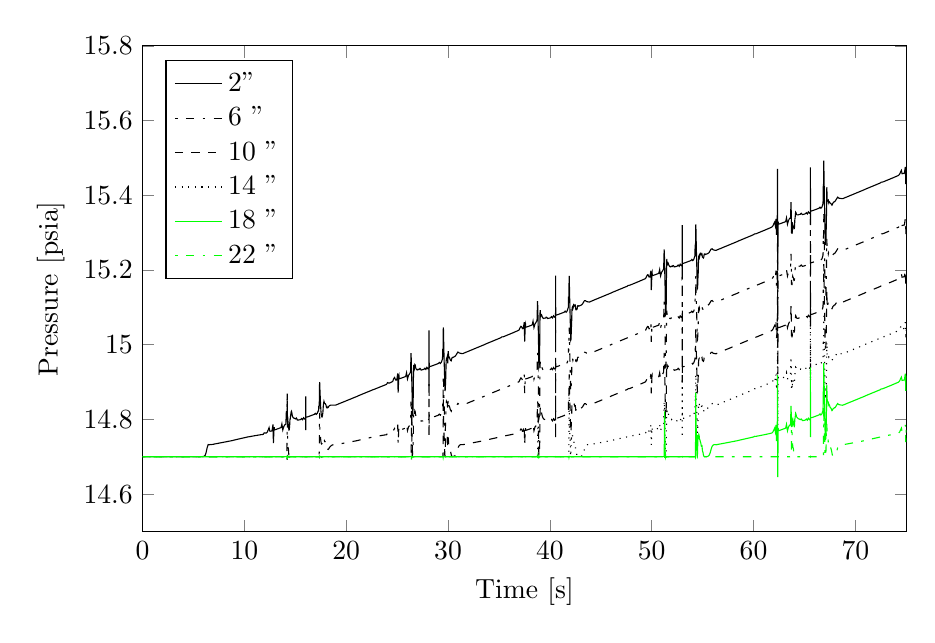
\begin{tikzpicture}

\begin{axis}[%
width=0.8\textwidth,
height=0.508815326102268\textwidth,
scale only axis,
xmin=0.0,
xmax=75,
xlabel={Time [s]},
ymin=14.5,
ymax=15.8,
ylabel={Pressure [psia]},
legend style={at={(0.03,0.97)},anchor=north west,draw=black,fill=white,legend cell align=left}
]
\addplot [
color=black,
solid
]
table[row sep=crcr]{
0 14.7007818222046\\
9.99999971718069e-10 14.7007818222046\\
2.49999998480632e-09 14.7007818222046\\
4.74999994892755e-09 14.7007818222046\\
8.1250002281763e-09 14.7007818222046\\
1.31874999809156e-08 14.7007818222046\\
2.0781250498203e-08 14.7007818222046\\
3.21718758300449e-08 14.7007818222046\\
4.92578138278077e-08 14.7007818222046\\
7.48867208244519e-08 14.7007818222046\\
1.13330081319418e-07 14.7007818222046\\
1.70995122061868e-07 14.7007818222046\\
2.57492672517401e-07 14.7007818222046\\
3.8723902662241e-07 14.7007818222046\\
5.81858500936505e-07 14.7007818222046\\
8.73787769251066e-07 14.7007818222046\\
1.31168167172291e-06 14.7007818222046\\
1.9685226106958e-06 14.7007827758789\\
2.95378367809462e-06 14.7007827758789\\
4.43167573394021e-06 14.7007827758789\\
6.64851359033491e-06 14.7007827758789\\
9.97376992017962e-06 14.7007837295532\\
1.49616553244414e-05 14.7007846832275\\
2.24434825213393e-05 14.7007856369019\\
3.36662233166862e-05 14.7007865905762\\
5.05003372381907e-05 14.7007884979248\\
7.57515081204474e-05 14.7007904052734\\
0.000113628258986864 14.7007932662964\\
0.000170443381648511 14.700795173645\\
0.000255666091106832 14.7007970809937\\
0.000383500126190484 14.7007970809937\\
0.000575251178815961 14.7007942199707\\
0.000862877757754177 14.7007904052734\\
0.00129431765526533 14.7007865905762\\
0.00194147753063589 14.7007837295532\\
0.00291221728548408 14.700779914856\\
0.00436832662671804 14.7007780075073\\
0.00597004732117057 14.700779914856\\
0.00773194013163447 14.7007827758789\\
0.009670021943748 14.7007837295532\\
0.0118019115179777 14.7007837295532\\
0.0141469910740852 14.7007827758789\\
0.0167265776544809 14.7007827758789\\
0.0195641238242388 14.7007827758789\\
0.0226854234933853 14.7007827758789\\
0.0261188540607691 14.7007827758789\\
0.0298956278711557 14.7007827758789\\
0.0340500771999359 14.7007827758789\\
0.0386199727654457 14.7007827758789\\
0.0436468608677387 14.7007827758789\\
0.0491764321923256 14.7007827758789\\
0.0552589632570744 14.7007827758789\\
0.0619497485458851 14.7007827758789\\
0.0693096145987511 14.7007827758789\\
0.0774054601788521 14.7007827758789\\
0.0863108932971954 14.700779914856\\
0.0961068719625473 14.7007827758789\\
0.106882445514202 14.7007827758789\\
0.118735581636429 14.7007827758789\\
0.13177402317524 14.7007827758789\\
0.146116316318512 14.7007827758789\\
0.161892831325531 14.7007827758789\\
0.179247006773949 14.7007827758789\\
0.198336601257324 14.7007827758789\\
0.21933513879776 14.7007827758789\\
0.242433547973633 14.7007827758789\\
0.267841786146164 14.7007827758789\\
0.29579085111618 14.7007827758789\\
0.32653483748436 14.7007827758789\\
0.360353201627731 14.7007827758789\\
0.397553414106369 14.7007837295532\\
0.438473641872406 14.7007837295532\\
0.483485877513886 14.7007837295532\\
0.532999336719513 14.7007837295532\\
0.587464153766632 14.7007837295532\\
0.647375464439392 14.7007837295532\\
0.71327793598175 14.7007837295532\\
0.7857705950737 14.7007837295532\\
0.865512549877167 14.7007837295532\\
0.953228712081909 14.7007837295532\\
1.04971647262573 14.7007837295532\\
1.14971649646759 14.7007827758789\\
1.24971640110016 14.7007827758789\\
1.34971642494202 14.7007827758789\\
1.44971644878387 14.7007827758789\\
1.54971647262573 14.7007827758789\\
1.64971649646759 14.7007827758789\\
1.74971640110016 14.7007827758789\\
1.84971642494202 14.7007827758789\\
1.94971644878387 14.7007827758789\\
2.04971647262573 14.7007827758789\\
2.1497163772583 14.7007827758789\\
2.24971652030945 14.7007827758789\\
2.34971642494202 14.7007827758789\\
2.44971656799316 14.7007827758789\\
2.54971647262573 14.7007827758789\\
2.6497163772583 14.7007827758789\\
2.74971652030945 14.7007827758789\\
2.84971642494202 14.7007827758789\\
2.94971656799316 14.7007827758789\\
3.04971647262573 14.7007827758789\\
3.1497163772583 14.7007827758789\\
3.24971652030945 14.7007827758789\\
3.34971642494202 14.7007827758789\\
3.44971656799316 14.7007827758789\\
3.54971647262573 14.7007827758789\\
3.6497163772583 14.7007827758789\\
3.74971652030945 14.7007827758789\\
3.84971642494202 14.7007827758789\\
3.94971656799316 14.7007827758789\\
4.04971647262573 14.7007827758789\\
4.1497163772583 14.7007827758789\\
4.24971628189087 14.7007827758789\\
4.3497166633606 14.7007827758789\\
4.44971656799316 14.7007827758789\\
4.54971647262573 14.7007827758789\\
4.6497163772583 14.7007827758789\\
4.74971628189087 14.7007827758789\\
4.8497166633606 14.7007827758789\\
4.94971656799316 14.7007827758789\\
5.04971647262573 14.7007837295532\\
5.1497163772583 14.7007837295532\\
5.24971628189087 14.7007837295532\\
5.3497166633606 14.7007837295532\\
5.44971656799316 14.7007837295532\\
5.54971647262573 14.7007837295532\\
5.6497163772583 14.7007837295532\\
5.74971628189087 14.7007884979248\\
5.8497166633606 14.7008085250854\\
5.94971656799316 14.70090675354\\
6.04971647262573 14.7014398574829\\
6.1497163772583 14.704080581665\\
6.24971628189087 14.7125511169434\\
6.3497166633606 14.725396156311\\
6.44971656799316 14.7330207824707\\
6.54971647262573 14.732325553894\\
6.6497163772583 14.733006477356\\
6.74971628189087 14.732626914978\\
6.8497166633606 14.7333736419678\\
6.94971656799316 14.7336568832397\\
7.04971647262573 14.734393119812\\
7.1497163772583 14.7347822189331\\
7.24971628189087 14.7354030609131\\
7.3497166633606 14.7358684539795\\
7.44971656799316 14.7364387512207\\
7.54971647262573 14.7369375228882\\
7.6497163772583 14.7374849319458\\
7.74971628189087 14.7379999160767\\
7.8497166633606 14.7385368347168\\
7.94971656799316 14.7390584945679\\
8.04971599578857 14.7395906448364\\
8.1497163772583 14.7401151657104\\
8.24971675872803 14.7406454086304\\
8.34971618652344 14.741171836853\\
8.44971656799316 14.7417011260986\\
8.54971599578857 14.7422285079956\\
8.6497163772583 14.7427568435669\\
8.74971675872803 14.7432851791382\\
8.84971618652344 14.743842124939\\
8.94971656799316 14.744704246521\\
9.04971599578857 14.7452869415283\\
9.1497163772583 14.7459402084351\\
9.24971675872803 14.7465677261353\\
9.34971618652344 14.7472019195557\\
9.44971656799316 14.7478313446045\\
9.54971599578857 14.748459815979\\
9.6497163772583 14.7490863800049\\
9.74971675872803 14.7497119903564\\
9.84971618652344 14.7503356933594\\
9.94971656799316 14.750958442688\\
10.0497159957886 14.751579284668\\
10.1497163772583 14.7521991729736\\
10.249716758728 14.752818107605\\
10.3497161865234 14.7534303665161\\
10.4497165679932 14.7537994384766\\
10.5497159957886 14.7542762756348\\
10.6497163772583 14.7548017501831\\
10.749716758728 14.7553043365479\\
10.8497161865234 14.7558059692383\\
10.9497165679932 14.7562980651855\\
11.0497159957886 14.7567825317383\\
11.1497163772583 14.7572574615479\\
11.249716758728 14.7577199935913\\
11.3497161865234 14.7581701278687\\
11.4497165679932 14.7586069107056\\
11.5497159957886 14.7590341567993\\
11.6497163772583 14.7594566345215\\
11.749716758728 14.7598266601563\\
11.8497161865234 14.7601566314697\\
11.9497165679932 14.7643003463745\\
12.0497159957886 14.7638158798218\\
12.1497163772583 14.7637815475464\\
12.249716758728 14.7665519714355\\
12.347146987915 14.7727012634277\\
12.4250946044922 14.7783174514771\\
12.4874591827393 14.7692184448242\\
12.5560598373413 14.7686729431152\\
12.6315202713013 14.7690563201904\\
12.714527130127 14.7695341110229\\
12.8058338165283 14.7866821289063\\
12.8497476577759 14.7367706298828\\
12.8980522155762 14.7679605484009\\
12.9143037796021 14.7766189575195\\
12.9277105331421 14.7797164916992\\
12.9424571990967 14.7722702026367\\
12.9586782455444 14.7723064422607\\
12.9765224456787 14.772406578064\\
12.9961500167847 14.7725305557251\\
13.0177412033081 14.77268409729\\
13.0414915084839 14.7728700637817\\
13.0676164627075 14.7730894088745\\
13.0963535308838 14.7733449935913\\
13.1279649734497 14.7736377716064\\
13.1627368927002 14.7739715576172\\
13.2009868621826 14.7743463516235\\
13.2430610656738 14.7747659683228\\
13.289342880249 14.7752323150635\\
13.3402528762817 14.7757482528687\\
13.3962545394897 14.7763185501099\\
13.4578561782837 14.7769460678101\\
13.5256175994873 14.7776365280151\\
13.600154876709 14.778395652771\\
13.6821460723877 14.7879543304443\\
13.7723369598389 14.7718334197998\\
13.871545791626 14.7812509536743\\
13.9715461730957 14.7859354019165\\
14.0715456008911 14.7874298095703\\
14.1215467453003 14.822286605835\\
14.1629066467285 14.8061380386353\\
14.2008075714111 14.8021659851074\\
14.202446937561 14.8055105209351\\
14.2042503356934 14.8240013122559\\
14.2062339782715 14.8408985137939\\
14.2084159851074 14.8495998382568\\
14.2108154296875 14.8495197296143\\
14.2134561538696 14.8429365158081\\
14.2163600921631 14.8314027786255\\
14.219554901123 14.8182067871094\\
14.223069190979 14.8070230484009\\
14.2269344329834 14.8084754943848\\
14.2311868667603 14.8092813491821\\
14.2358636856079 14.8092432022095\\
14.2410087585449 14.8087644577026\\
14.2466678619385 14.8074598312378\\
14.252893447876 14.8053932189941\\
14.2597417831421 14.8027753829956\\
14.2672748565674 14.7997331619263\\
14.2755603790283 14.7963581085205\\
14.2846755981445 14.7928276062012\\
14.2947015762329 14.7894258499146\\
14.3057298660278 14.7864694595337\\
14.3178615570068 14.7842407226563\\
14.3312063217163 14.781156539917\\
14.3458862304688 14.7773742675781\\
14.3620328903198 14.7738828659058\\
14.3797950744629 14.7717781066895\\
14.3993330001831 14.7722015380859\\
14.4208250045776 14.7758255004883\\
14.444465637207 14.7827854156494\\
14.4704713821411 14.7992000579834\\
14.4990768432617 14.8010311126709\\
14.5269069671631 14.8077249526978\\
14.5575199127197 14.8133459091187\\
14.591194152832 14.8202953338623\\
14.6282358169556 14.8221855163574\\
14.668981552124 14.8163824081421\\
14.7138023376465 14.8086853027344\\
14.7631044387817 14.8062963485718\\
14.8173370361328 14.8043746948242\\
14.8769931793213 14.8033285140991\\
14.9244384765625 14.8036556243896\\
14.971435546875 14.8023462295532\\
15.0163955688477 14.8014116287231\\
15.0584926605225 14.8017044067383\\
15.09974193573 14.8037843704224\\
15.1451168060303 14.8023767471313\\
15.1950283050537 14.7985095977783\\
15.2499313354492 14.798454284668\\
15.31032371521 14.7987003326416\\
15.3767566680908 14.7989416122437\\
15.4498319625854 14.7993688583374\\
15.5302152633667 14.7999668121338\\
15.6186370849609 14.8027420043945\\
15.7159004211426 14.7994613647461\\
15.8159008026123 14.8047113418579\\
15.9159002304077 14.8013105392456\\
16.0159015655518 14.8041286468506\\
16.0210952758789 14.8618545532227\\
16.0268077850342 14.7712955474854\\
16.0330924987793 14.8003377914429\\
16.0382099151611 14.8128252029419\\
16.0438404083252 14.8061847686768\\
16.0500316619873 14.8060998916626\\
16.0568428039551 14.8061246871948\\
16.0643348693848 14.8061370849609\\
16.0725765228271 14.8061580657959\\
16.0816440582275 14.806188583374\\
16.0916156768799 14.8062295913696\\
16.1025848388672 14.8062829971313\\
16.114652633667 14.8063507080078\\
16.1279258728027 14.8064346313477\\
16.1425266265869 14.8065366744995\\
16.1585865020752 14.806658744812\\
16.1762542724609 14.8068017959595\\
16.1956882476807 14.8069686889648\\
16.2170658111572 14.8071603775024\\
16.2405796051025 14.8073787689209\\
16.2664451599121 14.8076267242432\\
16.2948989868164 14.8079051971436\\
16.3261966705322 14.808217048645\\
16.3606243133545 14.8085632324219\\
16.398494720459 14.8089466094971\\
16.4401531219482 14.8093709945679\\
16.4859771728516 14.8098382949829\\
16.5363826751709 14.8103542327881\\
16.5918292999268 14.810920715332\\
16.6528205871582 14.8115453720093\\
16.7199096679688 14.8122320175171\\
16.7937088012695 14.8129873275757\\
16.8748874664307 14.8138189315796\\
16.9641857147217 14.8164825439453\\
17.0624122619629 14.813868522644\\
17.1624126434326 14.8169584274292\\
17.2624130249023 14.8240118026733\\
17.282413482666 14.823657989502\\
17.2906188964844 14.8352890014648\\
17.2996425628662 14.8353796005249\\
17.308614730835 14.8325834274292\\
17.3184852600098 14.8290567398071\\
17.3293399810791 14.8299474716187\\
17.3412818908691 14.8318319320679\\
17.3544178009033 14.8439884185791\\
17.3688678741455 14.8754425048828\\
17.3847618103027 14.900203704834\\
17.4022445678711 14.8964519500732\\
17.4214763641357 14.8773202896118\\
17.4426326751709 14.8638610839844\\
17.4659042358398 14.8489847183228\\
17.4915008544922 14.8338222503662\\
17.5196590423584 14.821475982666\\
17.5506324768066 14.8123626708984\\
17.5847034454346 14.807469367981\\
17.6221809387207 14.8068265914917\\
17.6634063720703 14.8099279403687\\
17.7087554931641 14.8187627792358\\
17.758638381958 14.8404922485352\\
17.8135089874268 14.8485536575317\\
17.8738670349121 14.842827796936\\
17.9402618408203 14.8422069549561\\
18.0132961273193 14.8383712768555\\
18.0585689544678 14.8328409194946\\
18.1083717346191 14.8343296051025\\
18.1509475708008 14.8309888839722\\
18.1891002655029 14.8310527801514\\
18.2310676574707 14.8325424194336\\
18.2772312164307 14.8346271514893\\
18.328010559082 14.8363342285156\\
18.3838691711426 14.8376054763794\\
18.4453125 14.8381900787354\\
18.5129013061523 14.8385066986084\\
18.5872478485107 14.838604927063\\
18.6690311431885 14.8386144638062\\
18.7589912414551 14.8385486602783\\
18.857946395874 14.8386554718018\\
18.9579467773438 14.8384847640991\\
19.0579471588135 14.8395795822144\\
19.1579456329346 14.8406105041504\\
19.2579460144043 14.841944694519\\
19.357946395874 14.842903137207\\
19.4579467773438 14.8440828323364\\
19.5579471588135 14.8451128005981\\
19.6579456329346 14.846266746521\\
19.7579460144043 14.8473405838013\\
19.857946395874 14.8484725952148\\
19.9579467773438 14.8495645523071\\
20.0579471588135 14.8506860733032\\
20.1579456329346 14.8517875671387\\
20.2579460144043 14.8529033660889\\
20.357946395874 14.8540096282959\\
20.4579467773438 14.8551225662231\\
20.5579471588135 14.8562459945679\\
20.6579456329346 14.8573503494263\\
20.7579460144043 14.8584671020508\\
20.857946395874 14.8595838546753\\
20.9579467773438 14.8607006072998\\
21.0579471588135 14.8618183135986\\
21.1579456329346 14.8630266189575\\
21.2579460144043 14.8643808364868\\
21.357946395874 14.8654346466064\\
21.4579467773438 14.8665714263916\\
21.5579471588135 14.8676843643188\\
21.6579456329346 14.8688049316406\\
21.7579460144043 14.8699235916138\\
21.857946395874 14.8710422515869\\
21.9579467773438 14.8721618652344\\
22.0579471588135 14.8732805252075\\
22.1579456329346 14.874400138855\\
22.2579460144043 14.8755197525024\\
22.357946395874 14.8766393661499\\
22.4579467773438 14.8777599334717\\
22.5579471588135 14.8788795471191\\
22.6579456329346 14.8799991607666\\
22.7579460144043 14.8809127807617\\
22.857946395874 14.8819284439087\\
22.9579467773438 14.8830671310425\\
23.0579471588135 14.8841619491577\\
23.1579456329346 14.8852710723877\\
23.2579460144043 14.8863725662231\\
23.357946395874 14.8874740600586\\
23.4579467773438 14.8885717391968\\
23.5579471588135 14.8896675109863\\
23.6579456329346 14.8907585144043\\
23.7579460144043 14.8918447494507\\
23.857946395874 14.8929300308228\\
23.9579467773438 14.8940086364746\\
24.0579471588135 14.8986959457397\\
24.1579456329346 14.8975744247437\\
24.2579460144043 14.897744178772\\
24.357946395874 14.8991279602051\\
24.4579467773438 14.900260925293\\
24.5579471588135 14.9015674591064\\
24.6579456329346 14.9091701507568\\
24.7421741485596 14.9124641418457\\
24.8095417022705 14.9085083007813\\
24.8836441040039 14.9052362442017\\
24.9651584625244 14.9058132171631\\
25.0548248291016 14.9230632781982\\
25.0960559844971 14.8717088699341\\
25.1414089202881 14.9016590118408\\
25.1613826751709 14.9160013198853\\
25.1780624389648 14.9176111221313\\
25.1964111328125 14.9090843200684\\
25.2165927886963 14.9091386795044\\
25.2387943267822 14.9092826843262\\
25.2632160186768 14.9094514846802\\
25.2900791168213 14.9096593856812\\
25.3196296691895 14.9099073410034\\
25.3521347045898 14.9101972579956\\
25.3878898620605 14.9105319976807\\
25.4272212982178 14.9109125137329\\
25.4704837799072 14.9113426208496\\
25.5180740356445 14.9118223190308\\
25.5704231262207 14.9123563766479\\
25.6280078887939 14.9129457473755\\
25.6913509368896 14.913595199585\\
25.7610282897949 14.9143095016479\\
25.8376731872559 14.9150953292847\\
25.9219818115234 14.9250659942627\\
26.014720916748 14.9083528518677\\
26.1147212982178 14.9180574417114\\
26.2147216796875 14.921932220459\\
26.3147220611572 14.927134513855\\
26.3647212982178 14.9778537750244\\
26.4022121429443 14.9465360641479\\
26.4049663543701 14.9284467697144\\
26.407995223999 14.935396194458\\
26.4113292694092 14.9388236999512\\
26.4149932861328 14.9347696304321\\
26.4190254211426 14.9316349029541\\
26.4234619140625 14.9242639541626\\
26.4283409118652 14.9146738052368\\
26.4337062835693 14.9070081710815\\
26.4396114349365 14.9011468887329\\
26.4461040496826 14.8947858810425\\
26.4532470703125 14.887113571167\\
26.4611053466797 14.8768863677979\\
26.469747543335 14.8629102706909\\
26.4792556762695 14.8461723327637\\
26.4897136688232 14.8287668228149\\
26.5012187957764 14.8169078826904\\
26.5138721466064 14.8114414215088\\
26.5277919769287 14.8120155334473\\
26.5431041717529 14.8180828094482\\
26.5599479675293 14.83216381073\\
26.5784759521484 14.8621435165405\\
26.59885597229 14.9094476699829\\
26.6212730407715 14.9460258483887\\
26.6459331512451 14.9301328659058\\
26.673059463501 14.9328136444092\\
26.7028980255127 14.9386129379272\\
26.7357215881348 14.9472522735596\\
26.7718257904053 14.9460687637329\\
26.8115406036377 14.9392356872559\\
26.8552284240723 14.935676574707\\
26.903284072876 14.9337797164917\\
26.9561443328857 14.9325113296509\\
27.0142917633057 14.9326648712158\\
27.0605869293213 14.9346504211426\\
27.1115131378174 14.933690071106\\
27.1556930541992 14.9336709976196\\
27.1975421905518 14.9352045059204\\
27.2435741424561 14.9364538192749\\
27.29421043396 14.9351358413696\\
27.3499088287354 14.932297706604\\
27.4111785888672 14.9325714111328\\
27.4785747528076 14.9331007003784\\
27.5527095794678 14.9335880279541\\
27.6342601776123 14.934289932251\\
27.7239646911621 14.9372901916504\\
27.8226375579834 14.9338979721069\\
27.9226379394531 14.9394845962524\\
28.0226383209229 14.9358282089233\\
28.1226387023926 14.9384756088257\\
28.1260833740234 15.0382537841797\\
28.1298713684082 14.8892765045166\\
28.1340389251709 14.9276351928711\\
28.1376724243164 15.0134801864624\\
28.1416683197021 14.8898229598999\\
28.1460647583008 14.9327945709229\\
28.1490650177002 14.9517526626587\\
28.1523666381836 14.9421472549438\\
28.1559963226318 14.9414167404175\\
28.1599903106689 14.9415578842163\\
28.1643829345703 14.9415702819824\\
28.1692161560059 14.9415721893311\\
28.1745319366455 14.9415788650513\\
28.1803779602051 14.9415903091431\\
28.1868114471436 14.9416065216064\\
28.1938858032227 14.94162940979\\
28.2016677856445 14.9416589736938\\
28.2102298736572 14.9416961669922\\
28.2196464538574 14.9417448043823\\
28.2300052642822 14.9418029785156\\
28.2413997650146 14.9418745040894\\
28.2539348602295 14.9419603347778\\
28.2677211761475 14.9420623779297\\
28.2828884124756 14.9421815872192\\
28.2995700836182 14.9423208236694\\
28.3179225921631 14.9424800872803\\
28.3381080627441 14.942663192749\\
28.3603134155273 14.94287109375\\
28.3847389221191 14.9431056976318\\
28.4116058349609 14.9433698654175\\
28.4411602020264 14.9436635971069\\
28.4736709594727 14.9439907073975\\
28.5094318389893 14.9443531036377\\
28.5487689971924 14.9447536468506\\
28.592041015625 14.9451961517334\\
28.6396389007568 14.9456825256348\\
28.6919975280762 14.9462194442749\\
28.7495918273926 14.9468097686768\\
28.8129444122314 14.9474592208862\\
28.8826332092285 14.9481735229492\\
28.9592895507813 14.9489593505859\\
29.0436134338379 14.9498233795166\\
29.1363677978516 14.9525756835938\\
29.2363681793213 14.9498739242554\\
29.336368560791 14.9530611038208\\
29.4363689422607 14.9611330032349\\
29.4563694000244 14.9623851776123\\
29.4642658233643 14.9859294891357\\
29.471960067749 14.9891338348389\\
29.4804267883301 14.9866094589233\\
29.4885120391846 14.9837093353271\\
29.497407913208 14.9834108352661\\
29.5071926116943 14.9845199584961\\
29.5179557800293 15.0109300613403\\
29.5297946929932 15.0415058135986\\
29.542818069458 15.0461511611938\\
29.5571441650391 15.0244150161743\\
29.5729026794434 15.0049772262573\\
29.5902366638184 14.9840297698975\\
29.6093044281006 14.9626836776733\\
29.630277633667 14.941764831543\\
29.6533489227295 14.9198904037476\\
29.6787281036377 14.8907403945923\\
29.6999015808105 14.876407623291\\
29.7231941223145 14.8805818557739\\
29.7488136291504 14.8946809768677\\
29.7769947052002 14.916898727417\\
29.8079967498779 14.9551162719727\\
29.8420963287354 14.9629096984863\\
29.8796062469482 14.964337348938\\
29.9208679199219 14.9686307907104\\
29.9662551879883 14.9501323699951\\
30.0161819458008 14.9829816818237\\
30.0711002349854 14.9656972885132\\
30.1315116882324 14.9662580490112\\
30.1804618835449 14.9625663757324\\
30.2286376953125 14.9588508605957\\
30.2746448516846 14.9575338363647\\
30.3156337738037 14.9569511413574\\
30.3508148193359 14.9623403549194\\
30.3895168304443 14.9652423858643\\
30.4320869445801 14.9663457870483\\
30.4789142608643 14.9659080505371\\
30.530424118042 14.9667615890503\\
30.587085723877 14.9676656723022\\
30.6491241455078 14.9685668945313\\
30.7173671722412 14.970085144043\\
30.7924346923828 14.9727687835693\\
30.8750076293945 14.9768199920654\\
30.9658393859863 14.9805240631104\\
31.0657539367676 14.9784851074219\\
31.1657543182373 14.9775447845459\\
31.265754699707 14.9767751693726\\
31.3657531738281 14.9764099121094\\
31.4657535552979 14.9764413833618\\
31.5657539367676 14.9777860641479\\
31.6657543182373 14.9787273406982\\
31.765754699707 14.9801406860352\\
31.8657531738281 14.9810800552368\\
31.9657535552979 14.9823312759399\\
32.0657539367676 14.9833765029907\\
32.1657524108887 14.9845590591431\\
32.265754699707 14.9856510162354\\
32.3657531738281 14.9868030548096\\
32.4657554626465 14.9879159927368\\
32.5657539367676 14.9890546798706\\
32.6657524108887 14.9901762008667\\
32.765754699707 14.9913234710693\\
32.8657531738281 14.9924306869507\\
32.9657554626465 14.9935617446899\\
33.0657539367676 14.9946889877319\\
33.1657524108887 14.9958181381226\\
33.265754699707 14.9969453811646\\
33.3657531738281 14.9980745315552\\
33.4657554626465 14.9992027282715\\
33.5657539367676 15.0003318786621\\
33.6657524108887 15.0017776489258\\
33.765754699707 15.0028581619263\\
33.8657531738281 15.0040016174316\\
33.9657554626465 15.0051259994507\\
34.0657539367676 15.0062570571899\\
34.1657524108887 15.0073852539063\\
34.265754699707 15.0085144042969\\
34.3657531738281 15.0096426010132\\
34.4657554626465 15.0107717514038\\
34.5657539367676 15.0118999481201\\
34.6657524108887 15.0130290985107\\
34.765754699707 15.0141572952271\\
34.8657531738281 15.0152864456177\\
34.9657554626465 15.016414642334\\
35.0657539367676 15.0175437927246\\
35.1657524108887 15.0185585021973\\
35.265754699707 15.0209302902222\\
35.3657531738281 15.021050453186\\
35.4657554626465 15.0217847824097\\
35.5657539367676 15.0230054855347\\
35.6657524108887 15.0240907669067\\
35.765754699707 15.0252275466919\\
35.8657531738281 15.0263442993164\\
35.9657554626465 15.0274677276611\\
36.0657539367676 15.0285882949829\\
36.1657524108887 15.029709815979\\
36.265754699707 15.0308656692505\\
36.3657531738281 15.0320091247559\\
36.4657554626465 15.0332450866699\\
36.5657539367676 15.0343761444092\\
36.6657524108887 15.0355224609375\\
36.765754699707 15.0367069244385\\
36.8657531738281 15.0379161834717\\
36.9657554626465 15.0391788482666\\
37.0657539367676 15.0455160140991\\
37.1539344787598 15.0494165420532\\
37.2244758605957 15.0481986999512\\
37.302074432373 15.0430421829224\\
37.3874282836914 15.0436573028564\\
37.4813194274902 15.0602931976318\\
37.5215835571289 15.0084915161133\\
37.5658721923828 15.0396490097046\\
37.585823059082 15.0534753799438\\
37.6024284362793 15.0553283691406\\
37.6206932067871 15.0469665527344\\
37.6407852172852 15.0470056533813\\
37.6628875732422 15.0471563339233\\
37.687198638916 15.0473251342773\\
37.713939666748 15.047532081604\\
37.7433547973633 15.047779083252\\
37.7757110595703 15.0480680465698\\
37.8113059997559 15.0484008789063\\
37.8504600524902 15.0487813949585\\
37.8935279846191 15.0492095947266\\
37.9409027099609 15.0496892929077\\
37.9930152893066 15.0502214431763\\
38.0503387451172 15.0508098602295\\
38.1133918762207 15.0514583587646\\
38.1827545166016 15.0521717071533\\
38.2590522766113 15.0529556274414\\
38.3429794311523 15.0630207061768\\
38.4352989196777 15.0461225509644\\
38.5352973937988 15.055908203125\\
38.6352996826172 15.0596828460693\\
38.7352981567383 15.0651807785034\\
38.7853012084961 15.1167736053467\\
38.822696685791 15.0908536911011\\
38.8252944946289 15.0733547210693\\
38.8281555175781 15.0774526596069\\
38.8313026428223 15.0795259475708\\
38.8347625732422 15.0770673751831\\
38.838565826416 15.0710439682007\\
38.8427543640137 15.0625610351563\\
38.8473587036133 15.0540237426758\\
38.852424621582 15.0471343994141\\
38.8579978942871 15.0409336090088\\
38.864128112793 15.0341482162476\\
38.8708724975586 15.0257711410522\\
38.878288269043 15.0134868621826\\
38.8864479064941 14.9969787597656\\
38.8954238891602 14.9751758575439\\
38.9052963256836 14.9578619003296\\
38.9161567687988 14.9400787353516\\
38.9281005859375 14.9417676925659\\
38.9412422180176 14.9435205459595\\
38.955696105957 14.9472627639771\\
38.9715957641602 14.955135345459\\
38.989086151123 14.9737100601196\\
39.0083236694336 15.0311689376831\\
39.029483795166 15.08482837677\\
39.0527648925781 15.0927820205688\\
39.078369140625 15.075701713562\\
39.1065368652344 15.0775184631348\\
39.137523651123 15.0812139511108\\
39.1716041564941 15.0810327529907\\
39.2090950012207 15.0780782699585\\
39.2477378845215 15.0748090744019\\
39.2902450561523 15.0725698471069\\
39.3370056152344 15.0710783004761\\
39.3884391784668 15.0702209472656\\
39.4450187683105 15.071102142334\\
39.4936180114746 15.0714464187622\\
39.5406875610352 15.071328163147\\
39.5853233337402 15.0714302062988\\
39.6272773742676 15.0737924575806\\
39.6734275817871 15.0737476348877\\
39.7241897583008 15.0724515914917\\
39.780029296875 15.0702171325684\\
39.8414497375488 15.0705289840698\\
39.9090156555176 15.0710573196411\\
39.9833374023438 15.0715703964233\\
40.0650939941406 15.0722875595093\\
40.1550216674805 15.0752973556519\\
40.2539443969727 15.0719032287598\\
40.353946685791 15.0775022506714\\
40.4539451599121 15.0738430023193\\
40.5539436340332 15.0763912200928\\
40.5569686889648 15.185115814209\\
40.5602951049805 15.0314807891846\\
40.5639533996582 15.0430164337158\\
40.5665168762207 15.1014156341553\\
40.5693359375 15.0995712280273\\
40.572437286377 15.0804147720337\\
40.5758476257324 15.078821182251\\
40.5796012878418 15.0795164108276\\
40.5837287902832 15.0796031951904\\
40.5882682800293 15.0795831680298\\
40.59326171875 15.0795783996582\\
40.5987548828125 15.0795812606812\\
40.6048011779785 15.0795869827271\\
40.6114463806152 15.0795993804932\\
40.6187591552734 15.0796175003052\\
40.6268005371094 15.0796432495117\\
40.6356506347656 15.0796785354614\\
40.6453819274902 15.0797243118286\\
40.6560897827148 15.0797815322876\\
40.6678657531738 15.079852104187\\
40.6808204650879 15.0799379348755\\
40.695068359375 15.0800409317017\\
40.7107429504395 15.0801630020142\\
40.7279853820801 15.0803050994873\\
40.7469482421875 15.0804691314697\\
40.7678108215332 15.0806579589844\\
40.7907600402832 15.0808734893799\\
40.8160057067871 15.0811157226563\\
40.8437728881836 15.0813884735107\\
40.8743171691895 15.0816926956177\\
40.9079170227051 15.08203125\\
40.9448776245117 15.0824069976807\\
40.9855308532715 15.0828218460083\\
41.0302505493164 15.0832786560059\\
41.0794448852539 15.0837831497192\\
41.1335563659668 15.0843372344971\\
41.1930809020996 15.0849475860596\\
41.2585563659668 15.0856199264526\\
41.3305778503418 15.0863580703735\\
41.4098052978516 15.0871706008911\\
41.4969520568848 15.0900230407715\\
41.5928153991699 15.0869903564453\\
41.692813873291 15.0902347564697\\
41.7928161621094 15.0984172821045\\
41.812816619873 15.1002035140991\\
41.8206024169922 15.1249942779541\\
41.8281707763672 15.1285877227783\\
41.8364944458008 15.1259145736694\\
41.8444328308105 15.1228017807007\\
41.8531684875488 15.1222820281982\\
41.8627777099609 15.122917175293\\
41.8733444213867 15.1460180282593\\
41.8849716186523 15.1806583404541\\
41.8977584838867 15.1841554641724\\
41.9118270874023 15.1632604598999\\
41.9272994995117 15.1431465148926\\
41.9443206787109 15.121753692627\\
41.9630432128906 15.100079536438\\
41.9836387634277 15.0787839889526\\
42.0062942504883 15.0537443161011\\
42.0312156677246 15.0245580673218\\
42.0477752685547 15.0123682022095\\
42.0659866333008 15.0136280059814\\
42.0860252380371 15.024938583374\\
42.1080627441406 15.0449419021606\\
42.1323051452637 15.0546989440918\\
42.1589736938477 15.0910930633545\\
42.1883087158203 15.0992889404297\\
42.2205772399902 15.1012601852417\\
42.2560729980469 15.0966300964355\\
42.2951164245605 15.1001777648926\\
42.3380661010742 15.1076736450195\\
42.3853073120117 15.1066675186157\\
42.4372749328613 15.1033849716187\\
42.494441986084 15.1053266525269\\
42.5416946411133 15.0951375961304\\
42.5936737060547 15.096531867981\\
42.6379699707031 15.0943431854248\\
42.6777877807617 15.0961751937866\\
42.711311340332 15.1033344268799\\
42.7481842041016 15.1048240661621\\
42.788745880127 15.1047687530518\\
42.833366394043 15.1033983230591\\
42.8824462890625 15.1040334701538\\
42.9364318847656 15.1046476364136\\
42.9958190917969 15.1051597595215\\
43.0611457824707 15.1059646606445\\
43.1330032348633 15.1072416305542\\
43.2120475769043 15.1095724105835\\
43.2989959716797 15.113748550415\\
43.3946380615234 15.1181840896606\\
43.4946365356445 15.1180944442749\\
43.5946388244629 15.1157741546631\\
43.694637298584 15.1150541305542\\
43.7946357727051 15.1145792007446\\
43.8946380615234 15.1145057678223\\
43.9946365356445 15.1158685684204\\
44.0946388244629 15.116792678833\\
44.194637298584 15.1182155609131\\
44.2946357727051 15.1191492080688\\
44.3946380615234 15.1204042434692\\
44.4946365356445 15.1214475631714\\
44.5946388244629 15.1226320266724\\
44.694637298584 15.1237230300903\\
44.7946357727051 15.1248760223389\\
44.8946380615234 15.1259880065918\\
44.9946365356445 15.1271266937256\\
45.0946388244629 15.1282634735107\\
45.194637298584 15.1293783187866\\
45.2946357727051 15.13050365448\\
45.3946380615234 15.1316337585449\\
45.4946365356445 15.1327610015869\\
45.5946388244629 15.1338901519775\\
45.694637298584 15.1350183486938\\
45.7946357727051 15.1361474990845\\
45.8946380615234 15.1372756958008\\
45.9946365356445 15.1384038925171\\
46.0946388244629 15.1398344039917\\
46.194637298584 15.1409349441528\\
46.2946357727051 15.1420736312866\\
46.3946380615234 15.14319896698\\
46.4946365356445 15.1443290710449\\
46.5946388244629 15.1454582214355\\
46.694637298584 15.1465864181519\\
46.7946357727051 15.1477155685425\\
46.8946380615234 15.1488437652588\\
46.9946365356445 15.1499729156494\\
47.0946388244629 15.15110206604\\
47.194637298584 15.1522302627563\\
47.2946357727051 15.153359413147\\
47.3946380615234 15.1544876098633\\
47.4946365356445 15.1556167602539\\
47.5946388244629 15.1566514968872\\
47.694637298584 15.1589956283569\\
47.7946357727051 15.1591262817383\\
47.8946380615234 15.159857749939\\
47.9946365356445 15.1610794067383\\
48.0946388244629 15.1621646881104\\
48.194637298584 15.1633014678955\\
48.2946357727051 15.16441822052\\
48.3946380615234 15.1655426025391\\
48.4946365356445 15.1666631698608\\
48.5946388244629 15.1677846908569\\
48.694637298584 15.1689376831055\\
48.7946357727051 15.1700830459595\\
48.8946380615234 15.1713132858276\\
48.9946365356445 15.1724462509155\\
49.0946388244629 15.1735925674438\\
49.194637298584 15.1747751235962\\
49.2946357727051 15.1759824752808\\
49.3946380615234 15.1772394180298\\
49.4946365356445 15.183144569397\\
49.5842514038086 15.1872692108154\\
49.6559371948242 15.1869163513184\\
49.7347946166992 15.1811637878418\\
49.8215370178223 15.1817903518677\\
49.9169502258301 15.1982421875\\
49.9568328857422 15.146143913269\\
50.0007057189941 15.1778249740601\\
50.0206336975098 15.1914901733398\\
50.0371971130371 15.1933851242065\\
50.0554161071777 15.185115814209\\
50.0754585266113 15.1851367950439\\
50.0975074768066 15.1852941513062\\
50.1217575073242 15.1854629516602\\
50.1484336853027 15.1856698989868\\
50.1777763366699 15.1859159469604\\
50.2100563049316 15.186203956604\\
50.2455635070801 15.1865367889404\\
50.2846183776855 15.186915397644\\
50.327579498291 15.1873426437378\\
50.3748397827148 15.1878204345703\\
50.4268226623535 15.1883516311646\\
50.4840087890625 15.1889390945435\\
50.5469093322754 15.18958568573\\
50.6161003112793 15.19029712677\\
50.692211151123 15.1910791397095\\
50.7759323120117 15.2011957168579\\
50.8680267333984 15.1841945648193\\
50.9680252075195 15.1940231323242\\
51.0680236816406 15.1977882385254\\
51.168025970459 15.2032928466797\\
51.2180252075195 15.2549610137939\\
51.2553977966309 15.2296571731567\\
51.2579727172852 15.2127141952515\\
51.2608032226563 15.2155904769897\\
51.263916015625 15.2179937362671\\
51.2673416137695 15.2154750823975\\
51.2711067199707 15.209321975708\\
51.2752532958984 15.2008104324341\\
51.2798080444336 15.1923246383667\\
51.2848243713379 15.1853818893433\\
51.290340423584 15.1792573928833\\
51.2964057922363 15.1724529266357\\
51.3030815124512 15.1639823913574\\
51.3104209899902 15.1515502929688\\
51.3184967041016 15.1346426010132\\
51.3273811340332 15.1127128601074\\
51.3371505737305 15.0955333709717\\
51.347900390625 15.0789575576782\\
51.3597221374512 15.0795888900757\\
51.372730255127 15.0811376571655\\
51.387035369873 15.0847425460815\\
51.4027709960938 15.0918245315552\\
51.4200820922852 15.1094789505005\\
51.4391212463379 15.1689157485962\\
51.4600677490234 15.2210750579834\\
51.4831085205078 15.2299270629883\\
51.5084533691406 15.2129240036011\\
51.5363311767578 15.2143421173096\\
51.5669975280762 15.2185926437378\\
51.6007308959961 15.2193460464478\\
51.6378364562988 15.2166843414307\\
51.6764678955078 15.2132549285889\\
51.7189598083496 15.2109603881836\\
51.7657051086426 15.2094097137451\\
51.8171195983887 15.2083053588867\\
51.8736801147461 15.2085933685303\\
51.9213600158691 15.2102651596069\\
51.9687728881836 15.2096061706543\\
52.0141105651855 15.2094478607178\\
52.056568145752 15.2113084793091\\
52.103271484375 15.2122058868408\\
52.1546440124512 15.2109136581421\\
52.2111549377441 15.208348274231\\
52.2733154296875 15.208643913269\\
52.3416938781738 15.2091865539551\\
52.4169082641602 15.2096929550171\\
52.4996490478516 15.2104158401489\\
52.5906600952148 15.2134113311768\\
52.6906585693359 15.2100734710693\\
52.790657043457 15.2156686782837\\
52.8906593322754 15.2120027542114\\
52.9906578063965 15.2145347595215\\
52.9936103820801 15.3199310302734\\
52.9968528747559 15.1782579421997\\
53.0004234313965 15.1784725189209\\
53.0029792785645 15.2348871231079\\
53.0057907104492 15.239634513855\\
53.0088844299316 15.2196378707886\\
53.0122871398926 15.2165288925171\\
53.0160293579102 15.2175464630127\\
53.0201454162598 15.2177867889404\\
53.0246734619141 15.2177562713623\\
53.0296516418457 15.2177438735962\\
53.0351333618164 15.2177457809448\\
53.0411605834961 15.2177515029907\\
53.0477867126465 15.2177629470825\\
53.0550804138184 15.2177810668945\\
53.063102722168 15.2178068161011\\
53.0719261169434 15.2178411483765\\
53.0816307067871 15.2178859710693\\
53.0923080444336 15.217942237854\\
53.1040496826172 15.2180118560791\\
53.1169700622559 15.2180976867676\\
53.1311798095703 15.2181997299194\\
53.1468124389648 15.2183208465576\\
53.164005279541 15.2184619903564\\
53.1829223632813 15.2186260223389\\
53.203727722168 15.2188138961792\\
53.2266120910645 15.2190275192261\\
53.2517852783203 15.2192697525024\\
53.2794799804688 15.2195415496826\\
53.3099403381348 15.2198448181152\\
53.343448638916 15.2201824188232\\
53.3803062438965 15.2205562591553\\
53.4208488464355 15.2209701538086\\
53.465446472168 15.2214260101318\\
53.5145034790039 15.2219285964966\\
53.5684700012207 15.2224817276001\\
53.6278305053711 15.223090171814\\
53.6931266784668 15.2237606048584\\
53.7649536132813 15.2244968414307\\
53.8439598083496 15.2253074645996\\
53.9308700561523 15.2281656265259\\
54.0264701843262 15.2251148223877\\
54.1264686584473 15.2283620834351\\
54.2264709472656 15.2365379333496\\
54.2464714050293 15.2386198043823\\
54.2542266845703 15.2631931304932\\
54.2617721557617 15.2669763565063\\
54.2700691223145 15.2642192840576\\
54.2779922485352 15.2610139846802\\
54.2867050170898 15.260425567627\\
54.2962913513184 15.26096534729\\
54.3068389892578 15.2839097976685\\
54.3184356689453 15.318567276001\\
54.3311958312988 15.322304725647\\
54.3452301025391 15.3014183044434\\
54.360668182373 15.281307220459\\
54.3776512145996 15.2599649429321\\
54.3963317871094 15.2383289337158\\
54.4168815612793 15.21706199646\\
54.4394836425781 15.1920490264893\\
54.4643478393555 15.1628932952881\\
54.4809799194336 15.1504936218262\\
54.4992752075195 15.1516256332397\\
54.519401550293 15.1630668640137\\
54.5415382385254 15.183177947998\\
54.5658912658691 15.193018913269\\
54.5926780700684 15.2295703887939\\
54.622142791748 15.2376203536987\\
54.6545562744141 15.2394208908081\\
54.6902084350586 15.2344551086426\\
54.7294273376465 15.2390375137329\\
54.7725677490234 15.2450160980225\\
54.8200225830078 15.2454128265381\\
54.8722229003906 15.2413148880005\\
54.9296417236328 15.2428646087646\\
54.9768371582031 15.2344007492065\\
55.028751373291 15.2336330413818\\
55.0732498168945 15.2323694229126\\
55.112865447998 15.2346811294556\\
55.1461601257324 15.241961479187\\
55.1827850341797 15.2431745529175\\
55.223072052002 15.2429599761963\\
55.2673873901367 15.2415571212769\\
55.3161315917969 15.2421951293945\\
55.3697547912598 15.2427835464478\\
55.4287376403809 15.243275642395\\
55.4936180114746 15.244047164917\\
55.5649871826172 15.2452487945557\\
55.643497467041 15.2474203109741\\
55.7298545837402 15.2514009475708\\
55.8248481750488 15.2560205459595\\
55.9248466491699 15.25670337677\\
56.024845123291 15.2540912628174\\
56.1248474121094 15.2533588409424\\
56.2248458862305 15.2528448104858\\
56.3248481750488 15.2526254653931\\
56.4248466491699 15.2539758682251\\
56.524845123291 15.2548961639404\\
56.6248474121094 15.2563190460205\\
56.7248458862305 15.2572526931763\\
56.8248481750488 15.2585077285767\\
56.9248466491699 15.2595510482788\\
57.024845123291 15.2607355117798\\
57.1248474121094 15.2618265151978\\
57.2248458862305 15.2629795074463\\
57.3248481750488 15.2640914916992\\
57.4248466491699 15.265230178833\\
57.524845123291 15.2663516998291\\
57.6248474121094 15.2674999237061\\
57.7248458862305 15.2686061859131\\
57.8248481750488 15.2697381973267\\
57.9248466491699 15.2708644866943\\
58.024845123291 15.271993637085\\
58.1248474121094 15.2731218338013\\
58.2248458862305 15.2742509841919\\
58.3248481750488 15.2753791809082\\
58.4248466491699 15.2765073776245\\
58.524845123291 15.2778968811035\\
58.6248474121094 15.2790489196777\\
58.7248458862305 15.2801733016968\\
58.8248481750488 15.2813034057617\\
58.9248466491699 15.2824325561523\\
59.024845123291 15.2835607528687\\
59.1248474121094 15.2846899032593\\
59.2248458862305 15.2858190536499\\
59.3248481750488 15.2869472503662\\
59.4248466491699 15.2880764007568\\
59.524845123291 15.2892045974731\\
59.6248474121094 15.2903337478638\\
59.7248458862305 15.2914628982544\\
59.8248481750488 15.2925910949707\\
59.9124221801758 15.2937297821045\\
60 15.29469871521\\
60.0963325500488 15.2968502044678\\
60.1963348388672 15.2969198226929\\
60.2963333129883 15.2976398468018\\
60.3963356018066 15.2988662719727\\
60.4963340759277 15.2999505996704\\
60.5963325500488 15.3010873794556\\
60.6963348388672 15.3022050857544\\
60.7963333129883 15.3033294677734\\
60.8963356018066 15.3044500350952\\
60.9963340759277 15.3055725097656\\
61.0963325500488 15.3067083358765\\
61.1963348388672 15.307861328125\\
61.2963333129883 15.3090677261353\\
61.3963356018066 15.3102102279663\\
61.4963340759277 15.3113584518433\\
61.5963325500488 15.3125314712524\\
61.6963348388672 15.3137254714966\\
61.7963333129883 15.314959526062\\
61.8963356018066 15.3182182312012\\
61.9940414428711 15.3241605758667\\
62.0722236633301 15.3283042907715\\
62.1347732543945 15.3189706802368\\
62.2035751342773 15.3367176055908\\
62.2478866577148 15.2942008972168\\
62.296630859375 15.3091068267822\\
62.3256530761719 15.3302955627441\\
62.3496742248535 15.4706392288208\\
62.376091003418 15.1986894607544\\
62.4051551818848 15.3181762695313\\
62.4213905334473 15.3258514404297\\
62.4340591430664 15.3262166976929\\
62.4479942321777 15.3228311538696\\
62.463321685791 15.3228530883789\\
62.4801826477051 15.3229732513428\\
62.4987297058105 15.3230962753296\\
62.5191307067871 15.3232421875\\
62.5415687561035 15.3234148025513\\
62.5662574768066 15.3236169815063\\
62.5934104919434 15.3238515853882\\
62.6232795715332 15.324122428894\\
62.656135559082 15.3244323730469\\
62.6922760009766 15.3247842788696\\
62.7320327758789 15.3251800537109\\
62.775764465332 15.3256235122681\\
62.8238677978516 15.3261165618896\\
62.8767852783203 15.32666015625\\
62.9349899291992 15.327260017395\\
62.9990196228027 15.327919960022\\
63.069450378418 15.3286447525024\\
63.1469230651855 15.3294410705566\\
63.2321434020996 15.3397207260132\\
63.3258857727051 15.3224306106567\\
63.4258842468262 15.3324546813965\\
63.5258865356445 15.3379039764404\\
63.6258850097656 15.3384323120117\\
63.6758842468262 15.3817491531372\\
63.7138481140137 15.3314323425293\\
63.7273941040039 15.2996273040771\\
63.7422943115234 15.3169603347778\\
63.7586822509766 15.3185386657715\\
63.7767105102539 15.2969207763672\\
63.7965431213379 15.3017091751099\\
63.8183555603027 15.3182992935181\\
63.8423538208008 15.3219213485718\\
63.8687477111816 15.318717956543\\
63.8977813720703 15.318018913269\\
63.9297218322754 15.3149900436401\\
63.9648513793945 15.3104887008667\\
64.0015869140625 15.3111572265625\\
64.022705078125 15.3167476654053\\
64.0459365844727 15.3334264755249\\
64.0714874267578 15.3389472961426\\
64.0996017456055 15.3463325500488\\
64.1305236816406 15.3547563552856\\
64.1645355224609 15.3535299301147\\
64.2019424438477 15.3490705490112\\
64.2431030273438 15.3479852676392\\
64.2883682250977 15.347713470459\\
64.3381729125977 15.347487449646\\
64.3929443359375 15.3475008010864\\
64.4477233886719 15.3484487533569\\
64.4993057250977 15.3487987518311\\
64.5481796264648 15.3489685058594\\
64.5940780639648 15.3492460250854\\
64.6370315551758 15.3512649536133\\
64.6842803955078 15.3517446517944\\
64.7362518310547 15.3502569198608\\
64.7934188842773 15.3483266830444\\
64.8563079833984 15.3486547470093\\
64.9254837036133 15.3492136001587\\
65.0015716552734 15.34974193573\\
65.0852737426758 15.3504848480225\\
65.1773452758789 15.3533477783203\\
65.27734375 15.350284576416\\
65.3773422241211 15.3556432723999\\
65.4773483276367 15.3522300720215\\
65.5773468017578 15.3544721603394\\
65.5794677734375 15.4745063781738\\
65.5817947387695 15.3445196151733\\
65.5843658447266 15.3259038925171\\
65.5871810913086 15.4183311462402\\
65.5902862548828 15.3203821182251\\
65.5937042236328 15.3265438079834\\
65.5974578857422 15.3662252426147\\
65.6015930175781 15.3682994842529\\
65.6061325073242 15.3584785461426\\
65.6111373901367 15.3575429916382\\
65.6166305541992 15.3578815460205\\
65.6226806640625 15.3579235076904\\
65.6293334960938 15.3579177856445\\
65.6366577148438 15.3579244613647\\
65.6447067260742 15.3579397201538\\
65.653564453125 15.3579635620117\\
65.6633071899414 15.3579988479614\\
65.6740188598633 15.3580465316772\\
65.6858062744141 15.3581075668335\\
65.6987762451172 15.3581857681274\\
65.7130355834961 15.3582801818848\\
65.7287292480469 15.3583946228027\\
65.7459869384766 15.35853099823\\
65.7649688720703 15.3586902618408\\
65.7858505249023 15.3588752746582\\
65.8088226318359 15.3590860366821\\
65.8340911865234 15.3593263626099\\
65.8618850708008 15.3595972061157\\
65.892463684082 15.3599004745483\\
65.9260940551758 15.3602380752563\\
65.9630889892578 15.3606128692627\\
66.0037841796875 15.3610277175903\\
66.0485458374023 15.3614854812622\\
66.097785949707 15.3619899749756\\
66.1519470214844 15.3625450134277\\
66.2115325927734 15.3631563186646\\
66.2770690917969 15.3638277053833\\
66.3491592407227 15.3645677566528\\
66.428466796875 15.3653812408447\\
66.5156936645508 15.3681468963623\\
66.6116485595703 15.3652858734131\\
66.7116470336914 15.3684387207031\\
66.811653137207 15.3778162002563\\
66.8316497802734 15.3898620605469\\
66.8391723632813 15.4199028015137\\
66.8464965820313 15.4246263504028\\
66.8545455932617 15.4207038879395\\
66.8622512817383 15.4169988632202\\
66.870735168457 15.4322299957275\\
66.8800659179688 15.4756212234497\\
66.8903274536133 15.4924879074097\\
66.9016189575195 15.4779796600342\\
66.9140319824219 15.4536113739014\\
66.9276962280273 15.4326419830322\\
66.9427185058594 15.4094114303589\\
66.9592437744141 15.384425163269\\
66.977424621582 15.3582563400269\\
66.997428894043 15.3190793991089\\
67.0194244384766 15.2925615310669\\
67.0415725708008 15.2754230499268\\
67.0659408569336 15.2683591842651\\
67.0927429199219 15.2687253952026\\
67.1222229003906 15.2986621856689\\
67.154655456543 15.345272064209\\
67.1903305053711 15.4217185974121\\
67.1995849609375 15.4155607223511\\
67.2097702026367 15.3985557556152\\
67.2209701538086 15.3900461196899\\
67.233283996582 15.3866586685181\\
67.2468414306641 15.385308265686\\
67.2617416381836 15.384801864624\\
67.2781448364258 15.3848314285278\\
67.2961807250977 15.385612487793\\
67.3160247802734 15.3863735198975\\
67.3378448486328 15.3816394805908\\
67.3618545532227 15.3846111297607\\
67.3882598876953 15.3821840286255\\
67.4173126220703 15.3834714889526\\
67.4492645263672 15.3825836181641\\
67.4844131469727 15.3801183700562\\
67.523078918457 15.3782930374146\\
67.5656127929688 15.3785448074341\\
67.6123962402344 15.3773174285889\\
67.6579818725586 15.3751306533813\\
67.6993789672852 15.3735256195068\\
67.7355346679688 15.3752956390381\\
67.7753067016602 15.3782510757446\\
67.8190612792969 15.3803510665894\\
67.8671875 15.381007194519\\
67.9201278686523 15.3830595016479\\
67.9783630371094 15.3832712173462\\
68.0421829223633 15.3856830596924\\
68.1070251464844 15.3884344100952\\
68.178352355957 15.3918466567993\\
68.2568130493164 15.3950309753418\\
68.3431243896484 15.3926219940186\\
68.4380569458008 15.3920574188232\\
68.5380630493164 15.3915920257568\\
68.6380615234375 15.3911762237549\\
68.7380599975586 15.3909158706665\\
68.8380584716797 15.3919887542725\\
68.9380569458008 15.3929557800293\\
69.0380630493164 15.3943405151367\\
69.1380615234375 15.3952960968018\\
69.2380599975586 15.3965358734131\\
69.3380584716797 15.3975887298584\\
69.4380569458008 15.3987655639648\\
69.5380630493164 15.3998613357544\\
69.6380615234375 15.40101146698\\
69.7380599975586 15.4021253585815\\
69.8380584716797 15.403263092041\\
69.9380569458008 15.4044008255005\\
70.0380630493164 15.4055147171021\\
70.1380615234375 15.4066410064697\\
70.2380599975586 15.4077701568604\\
70.3380584716797 15.4088983535767\\
70.4380569458008 15.4100275039673\\
70.5380630493164 15.4111557006836\\
70.6380615234375 15.4122838973999\\
70.7380599975586 15.4134120941162\\
70.8380584716797 15.4145412445068\\
70.9380569458008 15.4158201217651\\
71.0380630493164 15.4171123504639\\
71.1380615234375 15.4181985855103\\
71.2380599975586 15.419340133667\\
71.3380584716797 15.420464515686\\
71.4380569458008 15.421594619751\\
71.5380630493164 15.4227237701416\\
71.6380615234375 15.4238519668579\\
71.7380599975586 15.4249811172485\\
71.8380584716797 15.4261102676392\\
71.9380569458008 15.4272384643555\\
72.0380630493164 15.4283676147461\\
72.1380615234375 15.4294958114624\\
72.2380599975586 15.430624961853\\
72.3380584716797 15.4317531585693\\
72.4380569458008 15.4328804016113\\
72.5380630493164 15.4351453781128\\
72.6380615234375 15.435248374939\\
72.7380599975586 15.4360027313232\\
72.8380584716797 15.4372186660767\\
72.9380569458008 15.4383068084717\\
73.0380630493164 15.4394426345825\\
73.1380615234375 15.4405603408813\\
73.2380599975586 15.4416847229004\\
73.3380584716797 15.4428062438965\\
73.4380569458008 15.4439277648926\\
73.5380630493164 15.4450635910034\\
73.6380615234375 15.446216583252\\
73.7380599975586 15.4474229812622\\
73.8380584716797 15.4485664367676\\
73.9380569458008 15.4497146606445\\
74.0380630493164 15.4508867263794\\
74.1380615234375 15.4520797729492\\
74.2380599975586 15.453311920166\\
74.3380584716797 15.4563684463501\\
74.4363632202148 15.4624719619751\\
74.5150299072266 15.4665899276733\\
74.5779571533203 15.4576950073242\\
74.6471862792969 15.4580507278442\\
74.7233276367188 15.4585866928101\\
74.8070907592773 15.4592208862305\\
74.8992309570313 15.4758605957031\\
74.945930480957 15.4301147460938\\
74.9729614257813 15.4538860321045\\
74.9864807128906 15.469762802124\\
75 15.4706859588623\\
};
\addlegendentry{2"};

\addplot [
color=black,
dash pattern=on 1pt off 3pt on 3pt off 3pt
]
table[row sep=crcr]{
0 14.7006950378418\\
9.99999971718069e-10 14.7006950378418\\
2.49999998480632e-09 14.7006950378418\\
4.74999994892755e-09 14.7006950378418\\
8.1250002281763e-09 14.7006950378418\\
1.31874999809156e-08 14.7006950378418\\
2.0781250498203e-08 14.7006950378418\\
3.21718758300449e-08 14.7006950378418\\
4.92578138278077e-08 14.7006950378418\\
7.48867208244519e-08 14.7006950378418\\
1.13330081319418e-07 14.7006950378418\\
1.70995122061868e-07 14.7006950378418\\
2.57492672517401e-07 14.7006950378418\\
3.8723902662241e-07 14.7006950378418\\
5.81858500936505e-07 14.7006950378418\\
8.73787769251066e-07 14.7006950378418\\
1.31168167172291e-06 14.7006950378418\\
1.9685226106958e-06 14.7006950378418\\
2.95378367809462e-06 14.7006959915161\\
4.43167573394021e-06 14.7006959915161\\
6.64851359033491e-06 14.7006959915161\\
9.97376992017962e-06 14.7006959915161\\
1.49616553244414e-05 14.7006969451904\\
2.24434825213393e-05 14.7006978988647\\
3.36662233166862e-05 14.7006988525391\\
5.05003372381907e-05 14.7006998062134\\
7.57515081204474e-05 14.700701713562\\
0.000113628258986864 14.7007036209106\\
0.000170443381648511 14.7007055282593\\
0.000255666091106832 14.7007074356079\\
0.000383500126190484 14.7007083892822\\
0.000575251178815961 14.7007074356079\\
0.000862877757754177 14.7007036209106\\
0.00129431765526533 14.7007007598877\\
0.00194147753063589 14.7006969451904\\
0.00291221728548408 14.7006931304932\\
0.00436832662671804 14.7006912231445\\
0.00597004732117057 14.7006931304932\\
0.00773194013163447 14.7006950378418\\
0.009670021943748 14.7006959915161\\
0.0118019115179777 14.7006959915161\\
0.0141469910740852 14.7006959915161\\
0.0167265776544809 14.7006959915161\\
0.0195641238242388 14.7006959915161\\
0.0226854234933853 14.7006959915161\\
0.0261188540607691 14.7006959915161\\
0.0298956278711557 14.7006959915161\\
0.0340500771999359 14.7006959915161\\
0.0386199727654457 14.7006950378418\\
0.0436468608677387 14.7006950378418\\
0.0491764321923256 14.7006950378418\\
0.0552589632570744 14.7006950378418\\
0.0619497485458851 14.7006950378418\\
0.0693096145987511 14.7006959915161\\
0.0774054601788521 14.7006959915161\\
0.0863108932971954 14.7006931304932\\
0.0961068719625473 14.7006959915161\\
0.106882445514202 14.7006959915161\\
0.118735581636429 14.7006959915161\\
0.13177402317524 14.7006959915161\\
0.146116316318512 14.7006959915161\\
0.161892831325531 14.7006959915161\\
0.179247006773949 14.7006959915161\\
0.198336601257324 14.7006959915161\\
0.21933513879776 14.7006959915161\\
0.242433547973633 14.7006950378418\\
0.267841786146164 14.7006959915161\\
0.29579085111618 14.7006959915161\\
0.32653483748436 14.7006959915161\\
0.360353201627731 14.7006959915161\\
0.397553414106369 14.7006959915161\\
0.438473641872406 14.7006959915161\\
0.483485877513886 14.7006959915161\\
0.532999336719513 14.7006959915161\\
0.587464153766632 14.7006959915161\\
0.647375464439392 14.7006959915161\\
0.71327793598175 14.7006959915161\\
0.7857705950737 14.7006959915161\\
0.865512549877167 14.7006959915161\\
0.953228712081909 14.7006959915161\\
1.04971647262573 14.7006950378418\\
1.14971649646759 14.7006950378418\\
1.24971640110016 14.7006950378418\\
1.34971642494202 14.7006950378418\\
1.44971644878387 14.7006950378418\\
1.54971647262573 14.7006950378418\\
1.64971649646759 14.7006950378418\\
1.74971640110016 14.7006950378418\\
1.84971642494202 14.7006950378418\\
1.94971644878387 14.7006950378418\\
2.04971647262573 14.7006950378418\\
2.1497163772583 14.7006950378418\\
2.24971652030945 14.7006950378418\\
2.34971642494202 14.7006950378418\\
2.44971656799316 14.7006950378418\\
2.54971647262573 14.7006950378418\\
2.6497163772583 14.7006950378418\\
2.74971652030945 14.7006950378418\\
2.84971642494202 14.7006950378418\\
2.94971656799316 14.7006950378418\\
3.04971647262573 14.7006950378418\\
3.1497163772583 14.7006950378418\\
3.24971652030945 14.7006950378418\\
3.34971642494202 14.7006950378418\\
3.44971656799316 14.7006950378418\\
3.54971647262573 14.7006950378418\\
3.6497163772583 14.7006950378418\\
3.74971652030945 14.7006950378418\\
3.84971642494202 14.7006950378418\\
3.94971656799316 14.7006950378418\\
4.04971647262573 14.7006950378418\\
4.1497163772583 14.7006950378418\\
4.24971628189087 14.7006950378418\\
4.3497166633606 14.7006950378418\\
4.44971656799316 14.7006950378418\\
4.54971647262573 14.7006950378418\\
4.6497163772583 14.7006950378418\\
4.74971628189087 14.7006950378418\\
4.8497166633606 14.7006950378418\\
4.94971656799316 14.7006950378418\\
5.04971647262573 14.7006950378418\\
5.1497163772583 14.7006950378418\\
5.24971628189087 14.7006950378418\\
5.3497166633606 14.7006950378418\\
5.44971656799316 14.7006950378418\\
5.54971647262573 14.7006950378418\\
5.6497163772583 14.7006950378418\\
5.74971628189087 14.7006950378418\\
5.8497166633606 14.7006950378418\\
5.94971656799316 14.7006950378418\\
6.04971647262573 14.7006950378418\\
6.1497163772583 14.7006940841675\\
6.24971628189087 14.7006931304932\\
6.3497166633606 14.7006921768188\\
6.44971656799316 14.7006940841675\\
6.54971647262573 14.7006969451904\\
6.6497163772583 14.7006969451904\\
6.74971628189087 14.7006969451904\\
6.8497166633606 14.7006950378418\\
6.94971656799316 14.7006959915161\\
7.04971647262573 14.7006950378418\\
7.1497163772583 14.7006950378418\\
7.24971628189087 14.7006950378418\\
7.3497166633606 14.7006950378418\\
7.44971656799316 14.7006950378418\\
7.54971647262573 14.7006950378418\\
7.6497163772583 14.7006950378418\\
7.74971628189087 14.7006950378418\\
7.8497166633606 14.7006950378418\\
7.94971656799316 14.7006950378418\\
8.04971599578857 14.7006950378418\\
8.1497163772583 14.7006950378418\\
8.24971675872803 14.7006950378418\\
8.34971618652344 14.7006950378418\\
8.44971656799316 14.7006950378418\\
8.54971599578857 14.7006950378418\\
8.6497163772583 14.7006950378418\\
8.74971675872803 14.7006950378418\\
8.84971618652344 14.7006950378418\\
8.94971656799316 14.7006950378418\\
9.04971599578857 14.7006950378418\\
9.1497163772583 14.7006950378418\\
9.24971675872803 14.7006950378418\\
9.34971618652344 14.7006950378418\\
9.44971656799316 14.7006950378418\\
9.54971599578857 14.7006950378418\\
9.6497163772583 14.7006950378418\\
9.74971675872803 14.7006950378418\\
9.84971618652344 14.7006950378418\\
9.94971656799316 14.7006950378418\\
10.0497159957886 14.7006950378418\\
10.1497163772583 14.7006950378418\\
10.249716758728 14.7006950378418\\
10.3497161865234 14.7006950378418\\
10.4497165679932 14.7006950378418\\
10.5497159957886 14.7006950378418\\
10.6497163772583 14.7006950378418\\
10.749716758728 14.7006950378418\\
10.8497161865234 14.7006950378418\\
10.9497165679932 14.7006950378418\\
11.0497159957886 14.7006950378418\\
11.1497163772583 14.7006950378418\\
11.249716758728 14.7006950378418\\
11.3497161865234 14.7006950378418\\
11.4497165679932 14.7006950378418\\
11.5497159957886 14.7006950378418\\
11.6497163772583 14.7006959915161\\
11.749716758728 14.7006959915161\\
11.8497161865234 14.7006959915161\\
11.9497165679932 14.7006950378418\\
12.0497159957886 14.7006950378418\\
12.1497163772583 14.7006950378418\\
12.249716758728 14.7006950378418\\
12.347146987915 14.7006950378418\\
12.4250946044922 14.7006950378418\\
12.4874591827393 14.7006959915161\\
12.5560598373413 14.7006940841675\\
12.6315202713013 14.7006940841675\\
12.714527130127 14.7006950378418\\
12.8058338165283 14.7006959915161\\
12.8497476577759 14.7006959915161\\
12.8980522155762 14.7006950378418\\
12.9143037796021 14.7006959915161\\
12.9277105331421 14.7006978988647\\
12.9424571990967 14.7006978988647\\
12.9586782455444 14.7006969451904\\
12.9765224456787 14.7006969451904\\
12.9961500167847 14.7006959915161\\
13.0177412033081 14.7006959915161\\
13.0414915084839 14.7006959915161\\
13.0676164627075 14.7006959915161\\
13.0963535308838 14.7006959915161\\
13.1279649734497 14.7006959915161\\
13.1627368927002 14.7006959915161\\
13.2009868621826 14.7006959915161\\
13.2430610656738 14.7006959915161\\
13.289342880249 14.7006959915161\\
13.3402528762817 14.7006959915161\\
13.3962545394897 14.7006959915161\\
13.4578561782837 14.7006959915161\\
13.5256175994873 14.7006959915161\\
13.600154876709 14.7006959915161\\
13.6821460723877 14.7006959915161\\
13.7723369598389 14.7006969451904\\
13.871545791626 14.7006959915161\\
13.9715461730957 14.7007293701172\\
14.0715456008911 14.700870513916\\
14.1215467453003 14.7015914916992\\
14.1629066467285 14.7015705108643\\
14.2008075714111 14.7712888717651\\
14.202446937561 14.7973413467407\\
14.2042503356934 14.8541603088379\\
14.2062339782715 14.8689184188843\\
14.2084159851074 14.8619966506958\\
14.2108154296875 14.8516969680786\\
14.2134561538696 14.833625793457\\
14.2163600921631 14.8155269622803\\
14.219554901123 14.7990865707397\\
14.223069190979 14.7814884185791\\
14.2269344329834 14.7788047790527\\
14.2311868667603 14.7710580825806\\
14.2358636856079 14.764196395874\\
14.2410087585449 14.7578344345093\\
14.2466678619385 14.7517852783203\\
14.252893447876 14.7459573745728\\
14.2597417831421 14.7404403686523\\
14.2672748565674 14.7353935241699\\
14.2755603790283 14.7309741973877\\
14.2846755981445 14.727331161499\\
14.2947015762329 14.7246294021606\\
14.3057298660278 14.7229442596436\\
14.3178615570068 14.7221908569336\\
14.3312063217163 14.718150138855\\
14.3458862304688 14.7118816375732\\
14.3620328903198 14.7066335678101\\
14.3797950744629 14.7041082382202\\
14.3993330001831 14.7042331695557\\
14.4208250045776 14.7060146331787\\
14.444465637207 14.7087965011597\\
14.4704713821411 14.7034091949463\\
14.4990768432617 14.7011003494263\\
14.5269069671631 14.7006616592407\\
14.5575199127197 14.7006683349609\\
14.591194152832 14.7006826400757\\
14.6282358169556 14.7006950378418\\
14.668981552124 14.7007131576538\\
14.7138023376465 14.7007160186768\\
14.7631044387817 14.7007064819336\\
14.8173370361328 14.7007055282593\\
14.8769931793213 14.700704574585\\
14.9244384765625 14.7006988525391\\
14.971435546875 14.7006959915161\\
15.0163955688477 14.7006950378418\\
15.0584926605225 14.7006950378418\\
15.09974193573 14.7006940841675\\
15.1451168060303 14.7006940841675\\
15.1950283050537 14.7006959915161\\
15.2499313354492 14.7006950378418\\
15.31032371521 14.7006969451904\\
15.3767566680908 14.7006959915161\\
15.4498319625854 14.7006959915161\\
15.5302152633667 14.7006959915161\\
15.6186370849609 14.7006950378418\\
15.7159004211426 14.7006969451904\\
15.8159008026123 14.7006950378418\\
15.9159002304077 14.7006969451904\\
16.0159015655518 14.7006959915161\\
16.0210952758789 14.7006931304932\\
16.0268077850342 14.7007036209106\\
16.0330924987793 14.7006931304932\\
16.0382099151611 14.7006978988647\\
16.0438404083252 14.7006988525391\\
16.0500316619873 14.7006978988647\\
16.0568428039551 14.7006978988647\\
16.0643348693848 14.7006978988647\\
16.0725765228271 14.7006978988647\\
16.0816440582275 14.7006978988647\\
16.0916156768799 14.7006969451904\\
16.1025848388672 14.7006969451904\\
16.114652633667 14.7006969451904\\
16.1279258728027 14.7006969451904\\
16.1425266265869 14.7006969451904\\
16.1585865020752 14.7006969451904\\
16.1762542724609 14.7006969451904\\
16.1956882476807 14.7006969451904\\
16.2170658111572 14.7006969451904\\
16.2405796051025 14.7006969451904\\
16.2664451599121 14.7006969451904\\
16.2948989868164 14.7006969451904\\
16.3261966705322 14.7006969451904\\
16.3606243133545 14.7006969451904\\
16.398494720459 14.7006969451904\\
16.4401531219482 14.7006969451904\\
16.4859771728516 14.7006969451904\\
16.5363826751709 14.7006969451904\\
16.5918292999268 14.7006969451904\\
16.6528205871582 14.7006969451904\\
16.7199096679688 14.7006969451904\\
16.7937088012695 14.7006969451904\\
16.8748874664307 14.7006969451904\\
16.9641857147217 14.7006950378418\\
17.0624122619629 14.7006969451904\\
17.1624126434326 14.7006959915161\\
17.2624130249023 14.7007446289063\\
17.282413482666 14.7008991241455\\
17.2906188964844 14.7010221481323\\
17.2996425628662 14.7010688781738\\
17.308614730835 14.7010984420776\\
17.3184852600098 14.7011041641235\\
17.3293399810791 14.7011127471924\\
17.3412818908691 14.7024831771851\\
17.3544178009033 14.7275695800781\\
17.3688678741455 14.7853755950928\\
17.3847618103027 14.8174285888672\\
17.4022445678711 14.7983932495117\\
17.4214763641357 14.7616243362427\\
17.4426326751709 14.7631587982178\\
17.4659042358398 14.7555694580078\\
17.4915008544922 14.7472877502441\\
17.5196590423584 14.7405052185059\\
17.5506324768066 14.7360191345215\\
17.5847034454346 14.7344999313354\\
17.6221809387207 14.7355270385742\\
17.6634063720703 14.7383518218994\\
17.7087554931641 14.7449922561646\\
17.758638381958 14.7512359619141\\
17.8135089874268 14.7515563964844\\
17.8738670349121 14.7414798736572\\
17.9402618408203 14.739917755127\\
18.0132961273193 14.7363691329956\\
18.0585689544678 14.7272548675537\\
18.1083717346191 14.7288846969604\\
18.1509475708008 14.7240753173828\\
18.1891002655029 14.7205533981323\\
18.2310676574707 14.7198886871338\\
18.2772312164307 14.7213172912598\\
18.328010559082 14.72412109375\\
18.3838691711426 14.7261362075806\\
18.4453125 14.7280235290527\\
18.5129013061523 14.729790687561\\
18.5872478485107 14.7311811447144\\
18.6690311431885 14.7321882247925\\
18.7589912414551 14.7327442169189\\
18.857946395874 14.7330522537231\\
18.9579467773438 14.7327098846436\\
19.0579471588135 14.7331666946411\\
19.1579456329346 14.7335662841797\\
19.2579460144043 14.7342500686646\\
19.357946395874 14.7346525192261\\
19.4579467773438 14.7352237701416\\
19.5579471588135 14.7356719970703\\
19.6579456329346 14.736216545105\\
19.7579460144043 14.7366981506348\\
19.857946395874 14.7372255325317\\
19.9579467773438 14.7377214431763\\
20.0579471588135 14.7382392883301\\
20.1579456329346 14.7387428283691\\
20.2579460144043 14.7392578125\\
20.357946395874 14.7397651672363\\
20.4579467773438 14.7402782440186\\
20.5579471588135 14.7407932281494\\
20.6579456329346 14.7413101196289\\
20.7579460144043 14.7418270111084\\
20.857946395874 14.7423458099365\\
20.9579467773438 14.7428636550903\\
21.0579471588135 14.7433815002441\\
21.1579456329346 14.7439908981323\\
21.2579460144043 14.744779586792\\
21.357946395874 14.7453556060791\\
21.4579467773438 14.7459888458252\\
21.5579471588135 14.7466039657593\\
21.6579456329346 14.7472229003906\\
21.7579460144043 14.747838973999\\
21.857946395874 14.7484540939331\\
21.9579467773438 14.7490682601929\\
22.0579471588135 14.7496814727783\\
22.1579456329346 14.7502927780151\\
22.2579460144043 14.750904083252\\
22.357946395874 14.7515134811401\\
22.4579467773438 14.7521228790283\\
22.5579471588135 14.7527303695679\\
22.6579456329346 14.7533369064331\\
22.7579460144043 14.7537355422974\\
22.857946395874 14.7541751861572\\
22.9579467773438 14.7547063827515\\
23.0579471588135 14.7552003860474\\
23.1579456329346 14.7556991577148\\
23.2579460144043 14.7561874389648\\
23.357946395874 14.7566690444946\\
23.4579467773438 14.7571411132813\\
23.5579471588135 14.7576036453247\\
23.6579456329346 14.7580528259277\\
23.7579460144043 14.7584867477417\\
23.857946395874 14.7589073181152\\
23.9579467773438 14.7593097686768\\
24.0579471588135 14.7633056640625\\
24.1579456329346 14.7625570297241\\
24.2579460144043 14.7624015808105\\
24.357946395874 14.7632074356079\\
24.4579467773438 14.7638292312622\\
24.5579471588135 14.7646245956421\\
24.6579456329346 14.7717609405518\\
24.7421741485596 14.7758054733276\\
24.8095417022705 14.7720336914063\\
24.8836441040039 14.7685317993164\\
24.9651584625244 14.7689018249512\\
25.0548248291016 14.7859888076782\\
25.0960559844971 14.7341136932373\\
25.1414089202881 14.7641868591309\\
25.1613826751709 14.7782249450684\\
25.1780624389648 14.7797412872314\\
25.1964111328125 14.7712078094482\\
25.2165927886963 14.7712717056274\\
25.2387943267822 14.7714099884033\\
25.2632160186768 14.771577835083\\
25.2900791168213 14.7717838287354\\
25.3196296691895 14.7720289230347\\
25.3521347045898 14.7723159790039\\
25.3878898620605 14.772647857666\\
25.4272212982178 14.7730255126953\\
25.4704837799072 14.7734518051147\\
25.5180740356445 14.7739276885986\\
25.5704231262207 14.7744569778442\\
25.6280078887939 14.7750425338745\\
25.6913509368896 14.7756872177124\\
25.7610282897949 14.7763957977295\\
25.8376731872559 14.7771759033203\\
25.9219818115234 14.7871398925781\\
26.014720916748 14.7703218460083\\
26.1147212982178 14.7800798416138\\
26.2147216796875 14.783576965332\\
26.3147220611572 14.7887868881226\\
26.3647212982178 14.848048210144\\
26.4022121429443 14.8336534500122\\
26.4049663543701 14.8252029418945\\
26.407995223999 14.8308486938477\\
26.4113292694092 14.8344211578369\\
26.4149932861328 14.8308010101318\\
26.4190254211426 14.8281803131104\\
26.4234619140625 14.8212280273438\\
26.4283409118652 14.8120756149292\\
26.4337062835693 14.8048257827759\\
26.4396114349365 14.7993326187134\\
26.4461040496826 14.7933053970337\\
26.4532470703125 14.7859468460083\\
26.4611053466797 14.7760133743286\\
26.469747543335 14.7623176574707\\
26.4792556762695 14.7458114624023\\
26.4897136688232 14.7285528182983\\
26.5012187957764 14.716667175293\\
26.5138721466064 14.7106418609619\\
26.5277919769287 14.7095375061035\\
26.5431041717529 14.712498664856\\
26.5599479675293 14.7219457626343\\
26.5784759521484 14.7422571182251\\
26.59885597229 14.7919092178345\\
26.6212730407715 14.821683883667\\
26.6459331512451 14.8119859695435\\
26.673059463501 14.8118467330933\\
26.7028980255127 14.8162488937378\\
26.7357215881348 14.8232622146606\\
26.7718257904053 14.8208951950073\\
26.8115406036377 14.8129711151123\\
26.8552284240723 14.8080987930298\\
26.903284072876 14.8048315048218\\
26.9561443328857 14.8021869659424\\
27.0142917633057 14.8009271621704\\
27.0605869293213 14.8015432357788\\
27.1115131378174 14.799783706665\\
27.1556930541992 14.7989597320557\\
27.1975421905518 14.7998809814453\\
27.2435741424561 14.8006858825684\\
27.29421043396 14.7990341186523\\
27.3499088287354 14.7958717346191\\
27.4111785888672 14.7958831787109\\
27.4785747528076 14.7961912155151\\
27.5527095794678 14.7965116500854\\
27.6342601776123 14.7970752716064\\
27.7239646911621 14.7999620437622\\
27.8226375579834 14.796441078186\\
27.9226379394531 14.8019714355469\\
28.0226383209229 14.7982234954834\\
28.1226387023926 14.8008489608765\\
28.1260833740234 14.9006481170654\\
28.1298713684082 14.7492933273315\\
28.1340389251709 14.7903842926025\\
28.1376724243164 14.8755235671997\\
28.1416683197021 14.7502422332764\\
28.1460647583008 14.7953195571899\\
28.1490650177002 14.813307762146\\
28.1523666381836 14.8035535812378\\
28.1559963226318 14.803147315979\\
28.1599903106689 14.8032274246216\\
28.1643829345703 14.8032341003418\\
28.1692161560059 14.8032369613647\\
28.1745319366455 14.803243637085\\
28.1803779602051 14.8032541275024\\
28.1868114471436 14.8032703399658\\
28.1938858032227 14.8032932281494\\
28.2016677856445 14.8033227920532\\
28.2102298736572 14.8033609390259\\
28.2196464538574 14.8034076690674\\
28.2300052642822 14.803466796875\\
28.2413997650146 14.8035383224487\\
28.2539348602295 14.8036241531372\\
28.2677211761475 14.8037252426147\\
28.2828884124756 14.8038444519043\\
28.2995700836182 14.8039836883545\\
28.3179225921631 14.8041429519653\\
28.3381080627441 14.8043260574341\\
28.3603134155273 14.8045339584351\\
28.3847389221191 14.8047685623169\\
28.4116058349609 14.8050308227539\\
28.4411602020264 14.8053255081177\\
28.4736709594727 14.8056516647339\\
28.5094318389893 14.8060140609741\\
28.5487689971924 14.806414604187\\
28.592041015625 14.8068561553955\\
28.6396389007568 14.8073425292969\\
28.6919975280762 14.8078784942627\\
28.7495918273926 14.8084688186646\\
28.8129444122314 14.8091173171997\\
28.8826332092285 14.8098306655884\\
28.9592895507813 14.8106164932251\\
29.0436134338379 14.8114805221558\\
29.1363677978516 14.8142318725586\\
29.2363681793213 14.8115177154541\\
29.336368560791 14.8147134780884\\
29.4363689422607 14.8227472305298\\
29.4563694000244 14.825252532959\\
29.4642658233643 14.8501882553101\\
29.471960067749 14.8539094924927\\
29.4804267883301 14.8521890640259\\
29.4885120391846 14.8503618240356\\
29.497407913208 14.8512048721313\\
29.5071926116943 14.8537588119507\\
29.5179557800293 14.8819608688354\\
29.5297946929932 14.9143142700195\\
29.542818069458 14.9204559326172\\
29.5571441650391 14.9001007080078\\
29.5729026794434 14.8823947906494\\
29.5902366638184 14.8634014129639\\
29.6093044281006 14.844141960144\\
29.630277633667 14.8253393173218\\
29.6533489227295 14.8054790496826\\
29.6787281036377 14.7781705856323\\
29.6999015808105 14.765531539917\\
29.7231941223145 14.7706890106201\\
29.7488136291504 14.785083770752\\
29.7769947052002 14.8063268661499\\
29.8079967498779 14.8394737243652\\
29.8420963287354 14.8480978012085\\
29.8796062469482 14.845383644104\\
29.9208679199219 14.8454208374023\\
29.9662551879883 14.8260917663574\\
30.0161819458008 14.855565071106\\
30.0711002349854 14.8370428085327\\
30.1315116882324 14.8355121612549\\
30.1804618835449 14.830846786499\\
30.2286376953125 14.8257703781128\\
30.2746448516846 14.8235378265381\\
30.3156337738037 14.822135925293\\
30.3508148193359 14.8268299102783\\
30.3895168304443 14.8292980194092\\
30.4320869445801 14.8300714492798\\
30.4789142608643 14.8293828964233\\
30.530424118042 14.8300247192383\\
30.587085723877 14.8307418823242\\
30.6491241455078 14.8314914703369\\
30.7173671722412 14.8328800201416\\
30.7924346923828 14.8354530334473\\
30.8750076293945 14.8394088745117\\
30.9658393859863 14.8430318832397\\
31.0657539367676 14.8409242630005\\
31.1657543182373 14.8399267196655\\
31.265754699707 14.8391132354736\\
31.3657531738281 14.8387136459351\\
31.4657535552979 14.8387184143066\\
31.5657539367676 14.8400421142578\\
31.6657543182373 14.8409643173218\\
31.765754699707 14.8423614501953\\
31.8657531738281 14.8432855606079\\
31.9657535552979 14.844521522522\\
32.0657539367676 14.8455533981323\\
32.1657524108887 14.8467206954956\\
32.265754699707 14.8477993011475\\
32.3657531738281 14.8489370346069\\
32.4657554626465 14.8500356674194\\
32.5657539367676 14.8511610031128\\
32.6657524108887 14.8522691726685\\
32.765754699707 14.853404045105\\
32.8657531738281 14.8545045852661\\
32.9657554626465 14.8556299209595\\
33.0657539367676 14.8567495346069\\
33.1657524108887 14.8578729629517\\
33.265754699707 14.8589944839478\\
33.3657531738281 14.8601169586182\\
33.4657554626465 14.8612384796143\\
33.5657539367676 14.8623609542847\\
33.6657524108887 14.8638000488281\\
33.765754699707 14.8648748397827\\
33.8657531738281 14.8660125732422\\
33.9657554626465 14.867130279541\\
34.0657539367676 14.8682546615601\\
34.1657524108887 14.8693771362305\\
34.265754699707 14.8704996109009\\
34.3657531738281 14.8716220855713\\
34.4657554626465 14.872745513916\\
34.5657539367676 14.8738679885864\\
34.6657524108887 14.8749904632568\\
34.765754699707 14.8761138916016\\
34.8657531738281 14.877236366272\\
34.9657554626465 14.8783597946167\\
35.0657539367676 14.8794832229614\\
35.1657524108887 14.8804931640625\\
35.265754699707 14.8828592300415\\
35.3657531738281 14.8829736709595\\
35.4657554626465 14.8837022781372\\
35.5657539367676 14.8849182128906\\
35.6657524108887 14.8859987258911\\
35.765754699707 14.8871307373047\\
35.8657531738281 14.8882427215576\\
35.9657554626465 14.8893613815308\\
36.0657539367676 14.8904781341553\\
36.1657524108887 14.8915948867798\\
36.265754699707 14.8927459716797\\
36.3657531738281 14.8938865661621\\
36.4657554626465 14.8951177597046\\
36.5657539367676 14.8962450027466\\
36.6657524108887 14.8973865509033\\
36.765754699707 14.8985681533813\\
36.8657531738281 14.8997735977173\\
36.9657554626465 14.9010314941406\\
37.0657539367676 14.9073648452759\\
37.1539344787598 14.9112615585327\\
37.2244758605957 14.9100408554077\\
37.302074432373 14.904881477356\\
37.3874282836914 14.9054937362671\\
37.4813194274902 14.9221267700195\\
37.5215835571289 14.8703212738037\\
37.5658721923828 14.901478767395\\
37.585823059082 14.9153032302856\\
37.6024284362793 14.9171552658081\\
37.6206932067871 14.9087934494019\\
37.6407852172852 14.9088315963745\\
37.6628875732422 14.9089813232422\\
37.687198638916 14.9091501235962\\
37.713939666748 14.9093561172485\\
37.7433547973633 14.9096031188965\\
37.7757110595703 14.90989112854\\
37.8113059997559 14.9102230072021\\
37.8504600524902 14.9106016159058\\
37.8935279846191 14.9110298156738\\
37.9409027099609 14.9115076065063\\
37.9930152893066 14.9120388031006\\
38.0503387451172 14.9126262664795\\
38.1133918762207 14.913272857666\\
38.1827545166016 14.9139842987061\\
38.2590522766113 14.9147672653198\\
38.3429794311523 14.9248304367065\\
38.4352989196777 14.9079294204712\\
38.5352973937988 14.9177131652832\\
38.6352996826172 14.9214849472046\\
38.7352981567383 14.9269790649414\\
38.7853012084961 14.9785614013672\\
38.822696685791 14.9526319503784\\
38.8252944946289 14.9351177215576\\
38.8281555175781 14.9392414093018\\
38.8313026428223 14.9413003921509\\
38.8347625732422 14.9388408660889\\
38.838565826416 14.9328174591064\\
38.8427543640137 14.9243354797363\\
38.8473587036133 14.9157981872559\\
38.852424621582 14.9089088439941\\
38.8579978942871 14.9027090072632\\
38.864128112793 14.8959226608276\\
38.8708724975586 14.8875455856323\\
38.878288269043 14.8752603530884\\
38.8864479064941 14.8587512969971\\
38.8954238891602 14.8369483947754\\
38.9052963256836 14.8196353912354\\
38.9161567687988 14.801851272583\\
38.9281005859375 14.8035411834717\\
38.9412422180176 14.8052930831909\\
38.955696105957 14.8090343475342\\
38.9715957641602 14.8169059753418\\
38.989086151123 14.8354797363281\\
39.0083236694336 14.89293384552\\
39.029483795166 14.9465942382813\\
39.0527648925781 14.9545421600342\\
39.078369140625 14.937463760376\\
39.1065368652344 14.9392805099487\\
39.137523651123 14.9429740905762\\
39.1716041564941 14.9427919387817\\
39.2090950012207 14.9398365020752\\
39.2477378845215 14.9365653991699\\
39.2902450561523 14.9343252182007\\
39.3370056152344 14.9328317642212\\
39.3884391784668 14.9319725036621\\
39.4450187683105 14.9328527450562\\
39.4936180114746 14.9331951141357\\
39.5406875610352 14.9330749511719\\
39.5853233337402 14.9331750869751\\
39.6272773742676 14.9355363845825\\
39.6734275817871 14.935489654541\\
39.7241897583008 14.9341926574707\\
39.780029296875 14.931957244873\\
39.8414497375488 14.9322671890259\\
39.9090156555176 14.9327945709229\\
39.9833374023438 14.9333057403564\\
40.0650939941406 14.9340209960938\\
40.1550216674805 14.9370288848877\\
40.2539443969727 14.933632850647\\
40.353946685791 14.93922996521\\
40.4539451599121 14.9355688095093\\
40.5539436340332 14.9381160736084\\
40.5569686889648 15.0468902587891\\
40.5602951049805 14.8930931091309\\
40.5639533996582 14.9047975540161\\
40.5665168762207 14.963171005249\\
40.5693359375 14.9612560272217\\
40.572437286377 14.9421281814575\\
40.5758476257324 14.9405498504639\\
40.5796012878418 14.9412393569946\\
40.5837287902832 14.9413242340088\\
40.5882682800293 14.9413051605225\\
40.59326171875 14.9413003921509\\
40.5987548828125 14.9413022994995\\
40.6048011779785 14.9413089752197\\
40.6114463806152 14.9413204193115\\
40.6187591552734 14.9413385391235\\
40.6268005371094 14.9413642883301\\
40.6356506347656 14.9413995742798\\
40.6453819274902 14.9414443969727\\
40.6560897827148 14.9415016174316\\
40.6678657531738 14.9415721893311\\
40.6808204650879 14.9416580200195\\
40.695068359375 14.9417610168457\\
40.7107429504395 14.9418821334839\\
40.7279853820801 14.942024230957\\
40.7469482421875 14.9421882629395\\
40.7678108215332 14.9423770904541\\
40.7907600402832 14.9425916671753\\
40.8160057067871 14.9428339004517\\
40.8437728881836 14.9431056976318\\
40.8743171691895 14.9434099197388\\
40.9079170227051 14.9437475204468\\
40.9448776245117 14.9441223144531\\
40.9855308532715 14.9445362091064\\
41.0302505493164 14.944993019104\\
41.0794448852539 14.9454965591431\\
41.1335563659668 14.9460506439209\\
41.1930809020996 14.9466600418091\\
41.2585563659668 14.9473304748535\\
41.3305778503418 14.9480686187744\\
41.4098052978516 14.9488792419434\\
41.4969520568848 14.9517307281494\\
41.5928153991699 14.9486961364746\\
41.692813873291 14.9519386291504\\
41.7928161621094 14.9601202011108\\
41.812816619873 14.9618997573853\\
41.8206024169922 14.9866905212402\\
41.8281707763672 14.9902801513672\\
41.8364944458008 14.9876079559326\\
41.8444328308105 14.9844951629639\\
41.8531684875488 14.9839754104614\\
41.8627777099609 14.9846096038818\\
41.8733444213867 15.0077123641968\\
41.8849716186523 15.042350769043\\
41.8977584838867 15.0458459854126\\
41.9118270874023 15.0249519348145\\
41.9272994995117 15.0048379898071\\
41.9443206787109 14.9834451675415\\
41.9630432128906 14.9617710113525\\
41.9836387634277 14.9404754638672\\
42.0062942504883 14.9154348373413\\
42.0312156677246 14.886248588562\\
42.0477752685547 14.8740587234497\\
42.0659866333008 14.8753185272217\\
42.0860252380371 14.8866281509399\\
42.1080627441406 14.9066314697266\\
42.1323051452637 14.9163885116577\\
42.1589736938477 14.9527816772461\\
42.1883087158203 14.960976600647\\
42.2205772399902 14.9629468917847\\
42.2560729980469 14.9583158493042\\
42.2951164245605 14.9618625640869\\
42.3380661010742 14.9693574905396\\
42.3853073120117 14.9683485031128\\
42.4372749328613 14.9650659561157\\
42.494441986084 14.9670066833496\\
42.5416946411133 14.9568157196045\\
42.5936737060547 14.9582090377808\\
42.6379699707031 14.956018447876\\
42.6777877807617 14.9578504562378\\
42.711311340332 14.9650087356567\\
42.7481842041016 14.9664974212646\\
42.788745880127 14.96644115448\\
42.833366394043 14.965069770813\\
42.8824462890625 14.9657049179077\\
42.9364318847656 14.9663181304932\\
42.9958190917969 14.9668292999268\\
43.0611457824707 14.9676332473755\\
43.1330032348633 14.9689092636108\\
43.2120475769043 14.9712390899658\\
43.2989959716797 14.9754133224487\\
43.3946380615234 14.97984790802\\
43.4946365356445 14.9797563552856\\
43.5946388244629 14.9774351119995\\
43.694637298584 14.9767141342163\\
43.7946357727051 14.9762372970581\\
43.8946380615234 14.9761629104614\\
43.9946365356445 14.9775247573853\\
44.0946388244629 14.9784469604492\\
44.194637298584 14.9798679351807\\
44.2946357727051 14.9808006286621\\
44.3946380615234 14.9820547103882\\
44.4946365356445 14.983097076416\\
44.5946388244629 14.9842796325684\\
44.694637298584 14.985369682312\\
44.7946357727051 14.9865217208862\\
44.8946380615234 14.9876327514648\\
44.9946365356445 14.9887704849243\\
45.0946388244629 14.9899053573608\\
45.194637298584 14.9910192489624\\
45.2946357727051 14.9921436309814\\
45.3946380615234 14.9932727813721\\
45.4946365356445 14.9943990707397\\
45.5946388244629 14.9955272674561\\
45.694637298584 14.9966535568237\\
45.7946357727051 14.99778175354\\
45.8946380615234 14.998908996582\\
45.9946365356445 15.000036239624\\
46.0946388244629 15.0014657974243\\
46.194637298584 15.0025653839111\\
46.2946357727051 15.0037021636963\\
46.3946380615234 15.0048274993896\\
46.4946365356445 15.0059566497803\\
46.5946388244629 15.0070838928223\\
46.694637298584 15.0082120895386\\
46.7946357727051 15.0093393325806\\
46.8946380615234 15.0104675292969\\
46.9946365356445 15.0115947723389\\
47.0946388244629 15.0127229690552\\
47.194637298584 15.0138502120972\\
47.2946357727051 15.0149784088135\\
47.3946380615234 15.0161056518555\\
47.4946365356445 15.0172338485718\\
47.5946388244629 15.0182676315308\\
47.694637298584 15.0206108093262\\
47.7946357727051 15.0207405090332\\
47.8946380615234 15.0214710235596\\
47.9946365356445 15.0226926803589\\
48.0946388244629 15.0237770080566\\
48.194637298584 15.0249128341675\\
48.2946357727051 15.0260286331177\\
48.3946380615234 15.0271511077881\\
48.4946365356445 15.0282716751099\\
48.5946388244629 15.0293922424316\\
48.694637298584 15.0305442810059\\
48.7946357727051 15.0316886901855\\
48.8946380615234 15.0329189300537\\
48.9946365356445 15.034049987793\\
49.0946388244629 15.0351963043213\\
49.194637298584 15.0363779067993\\
49.2946357727051 15.0375843048096\\
49.3946380615234 15.0388402938843\\
49.4946365356445 15.0447454452515\\
49.5842514038086 15.0488681793213\\
49.6559371948242 15.0485153198242\\
49.7347946166992 15.0427618026733\\
49.8215370178223 15.0433874130249\\
49.9169502258301 15.0598392486572\\
49.9568328857422 15.0077390670776\\
50.0007057189941 15.039421081543\\
50.0206336975098 15.0530853271484\\
50.0371971130371 15.0549802780151\\
50.0554161071777 15.0467109680176\\
50.0754585266113 15.0467319488525\\
50.0975074768066 15.0468893051147\\
50.1217575073242 15.0470581054688\\
50.1484336853027 15.0472650527954\\
50.1777763366699 15.047511100769\\
50.2100563049316 15.0477981567383\\
50.2455635070801 15.0481300354004\\
50.2846183776855 15.048508644104\\
50.327579498291 15.0489358901978\\
50.3748397827148 15.0494136810303\\
50.4268226623535 15.0499439239502\\
50.4840087890625 15.0505313873291\\
50.5469093322754 15.0511770248413\\
50.6161003112793 15.0518884658813\\
50.692211151123 15.0526704788208\\
50.7759323120117 15.0627861022949\\
50.8680267333984 15.0457849502563\\
50.9680252075195 15.0556125640869\\
51.0680236816406 15.0593776702881\\
51.168025970459 15.0648803710938\\
51.2180252075195 15.116548538208\\
51.2553977966309 15.0912437438965\\
51.2579727172852 15.0742902755737\\
51.2608032226563 15.0771884918213\\
51.263916015625 15.0795803070068\\
51.2673416137695 15.0770597457886\\
51.2711067199707 15.0709066390991\\
51.2752532958984 15.0623970031738\\
51.2798080444336 15.0539112091064\\
51.2848243713379 15.0469694137573\\
51.290340423584 15.040843963623\\
51.2964057922363 15.0340385437012\\
51.3030815124512 15.0255680084229\\
51.3104209899902 15.0131368637085\\
51.3184967041016 14.9962282180786\\
51.3273811340332 14.9742994308472\\
51.3371505737305 14.9571199417114\\
51.347900390625 14.940544128418\\
51.3597221374512 14.9411754608154\\
51.372730255127 14.9427242279053\\
51.387035369873 14.9463291168213\\
51.4027709960938 14.9534101486206\\
51.4200820922852 14.9710655212402\\
51.4391212463379 15.0305023193359\\
51.4600677490234 15.0826597213745\\
51.4831085205078 15.0915117263794\\
51.5084533691406 15.0745086669922\\
51.5363311767578 15.075927734375\\
51.5669975280762 15.0801773071289\\
51.6007308959961 15.0809307098389\\
51.6378364562988 15.0782690048218\\
51.6764678955078 15.0748386383057\\
51.7189598083496 15.0725440979004\\
51.7657051086426 15.0709924697876\\
51.8171195983887 15.0698881149292\\
51.8736801147461 15.0701761245728\\
51.9213600158691 15.0718479156494\\
51.9687728881836 15.0711879730225\\
52.0141105651855 15.0710296630859\\
52.056568145752 15.0728902816772\\
52.103271484375 15.0737867355347\\
52.1546440124512 15.0724945068359\\
52.2111549377441 15.0699281692505\\
52.2733154296875 15.0702238082886\\
52.3416938781738 15.0707664489746\\
52.4169082641602 15.0712728500366\\
52.4996490478516 15.0719947814941\\
52.5906600952148 15.074990272522\\
52.6906585693359 15.0716514587402\\
52.790657043457 15.0772457122803\\
52.8906593322754 15.073579788208\\
52.9906578063965 15.0761108398438\\
52.9936103820801 15.1815595626831\\
52.9968528747559 15.0397243499756\\
53.0004234313965 15.0401020050049\\
53.0029792785645 15.0965013504028\\
53.0057907104492 15.1011781692505\\
53.0088844299316 15.081202507019\\
53.0122871398926 15.0781116485596\\
53.0160293579102 15.079122543335\\
53.0201454162598 15.0793619155884\\
53.0246734619141 15.0793313980103\\
53.0296516418457 15.0793190002441\\
53.0351333618164 15.0793209075928\\
53.0411605834961 15.079327583313\\
53.0477867126465 15.0793380737305\\
53.0550804138184 15.0793561935425\\
53.063102722168 15.079381942749\\
53.0719261169434 15.0794162750244\\
53.0816307067871 15.0794610977173\\
53.0923080444336 15.079517364502\\
53.1040496826172 15.0795869827271\\
53.1169700622559 15.0796728134155\\
53.1311798095703 15.0797748565674\\
53.1468124389648 15.0798959732056\\
53.164005279541 15.0800371170044\\
53.1829223632813 15.0802001953125\\
53.203727722168 15.0803880691528\\
53.2266120910645 15.080602645874\\
53.2517852783203 15.0808439254761\\
53.2794799804688 15.0811157226563\\
53.3099403381348 15.0814189910889\\
53.343448638916 15.0817565917969\\
53.3803062438965 15.0821304321289\\
53.4208488464355 15.0825433731079\\
53.465446472168 15.0829992294312\\
53.5145034790039 15.0835018157959\\
53.5684700012207 15.0840539932251\\
53.6278305053711 15.0846633911133\\
53.6931266784668 15.0853319168091\\
53.7649536132813 15.0860691070557\\
53.8439598083496 15.0868787765503\\
53.9308700561523 15.0897359848022\\
54.0264701843262 15.0866851806641\\
54.1264686584473 15.0899314880371\\
54.2264709472656 15.0981073379517\\
54.2464714050293 15.1001882553101\\
54.2542266845703 15.1247634887695\\
54.2617721557617 15.1285429000854\\
54.2700691223145 15.1257877349854\\
54.2779922485352 15.1225824356079\\
54.2867050170898 15.1219940185547\\
54.2962913513184 15.1225337982178\\
54.3068389892578 15.1454792022705\\
54.3184356689453 15.1801357269287\\
54.3311958312988 15.1838722229004\\
54.3452301025391 15.1629858016968\\
54.360668182373 15.1428747177124\\
54.3776512145996 15.1215333938599\\
54.3963317871094 15.0998964309692\\
54.4168815612793 15.0786294937134\\
54.4394836425781 15.0536165237427\\
54.4643478393555 15.0244607925415\\
54.4809799194336 15.0120620727539\\
54.4992752075195 15.0131940841675\\
54.519401550293 15.0246343612671\\
54.5415382385254 15.0447454452515\\
54.5658912658691 15.0545864105225\\
54.5926780700684 15.0911378860474\\
54.622142791748 15.0991878509521\\
54.6545562744141 15.1009874343872\\
54.6902084350586 15.0960216522217\\
54.7294273376465 15.100604057312\\
54.7725677490234 15.1065816879272\\
54.8200225830078 15.1069784164429\\
54.8722229003906 15.1028804779053\\
54.9296417236328 15.1044301986694\\
54.9768371582031 15.095965385437\\
55.028751373291 15.0951986312866\\
55.0732498168945 15.0939340591431\\
55.112865447998 15.096245765686\\
55.1461601257324 15.1035261154175\\
55.1827850341797 15.1047391891479\\
55.223072052002 15.1045246124268\\
55.2673873901367 15.103120803833\\
55.3161315917969 15.1037588119507\\
55.3697547912598 15.1043462753296\\
55.4287376403809 15.1048393249512\\
55.4936180114746 15.1056108474731\\
55.5649871826172 15.1068115234375\\
55.643497467041 15.1089820861816\\
55.7298545837402 15.1129627227783\\
55.8248481750488 15.1175813674927\\
55.9248466491699 15.1182641983032\\
56.024845123291 15.1156520843506\\
56.1248474121094 15.1149187088013\\
56.2248458862305 15.1144046783447\\
56.3248481750488 15.114185333252\\
56.4248466491699 15.1155347824097\\
56.524845123291 15.116455078125\\
56.6248474121094 15.1178770065308\\
56.7248458862305 15.1188097000122\\
56.8248481750488 15.1200647354126\\
56.9248466491699 15.1211080551147\\
57.024845123291 15.1222915649414\\
57.1248474121094 15.1233825683594\\
57.2248458862305 15.1245346069336\\
57.3248481750488 15.1256465911865\\
57.4248466491699 15.1267852783203\\
57.524845123291 15.1279058456421\\
57.6248474121094 15.1290531158447\\
57.7248458862305 15.1301603317261\\
57.8248481750488 15.131290435791\\
57.9248466491699 15.1324167251587\\
58.024845123291 15.1335458755493\\
58.1248474121094 15.1346731185913\\
58.2248458862305 15.1358022689819\\
58.3248481750488 15.1369295120239\\
58.4248466491699 15.1380586624146\\
58.524845123291 15.1394472122192\\
58.6248474121094 15.1405992507935\\
58.7248458862305 15.1417226791382\\
58.8248481750488 15.1428527832031\\
58.9248466491699 15.1439809799194\\
59.024845123291 15.1451091766357\\
59.1248474121094 15.1462383270264\\
59.2248458862305 15.1473665237427\\
59.3248481750488 15.148494720459\\
59.4248466491699 15.1496229171753\\
59.524845123291 15.1507520675659\\
59.6248474121094 15.1518802642822\\
59.7248458862305 15.1530084609985\\
59.8248481750488 15.1541366577148\\
59.9124221801758 15.1552743911743\\
60 15.1562433242798\\
60.0963325500488 15.1583948135376\\
60.1963348388672 15.1584644317627\\
60.2963333129883 15.1591835021973\\
60.3963356018066 15.1604099273682\\
60.4963340759277 15.1614933013916\\
60.5963325500488 15.1626310348511\\
60.6963348388672 15.1637477874756\\
60.7963333129883 15.1648712158203\\
60.8963356018066 15.1659927368164\\
60.9963340759277 15.1671142578125\\
61.0963325500488 15.1682500839233\\
61.1963348388672 15.1694021224976\\
61.2963333129883 15.1706085205078\\
61.3963356018066 15.1717510223389\\
61.4963340759277 15.1728992462158\\
61.5963325500488 15.1740713119507\\
61.6963348388672 15.1752653121948\\
61.7963333129883 15.1764984130859\\
61.8963356018066 15.1797571182251\\
61.9940414428711 15.1856994628906\\
62.0722236633301 15.1898422241211\\
62.1347732543945 15.1805095672607\\
62.2035751342773 15.1982555389404\\
62.2478866577148 15.1557388305664\\
62.296630859375 15.1706457138062\\
62.3256530761719 15.1918334960938\\
62.3496742248535 15.3321781158447\\
62.376091003418 15.0602235794067\\
62.4051551818848 15.1797170639038\\
62.4213905334473 15.187388420105\\
62.4340591430664 15.1877546310425\\
62.4479942321777 15.1843690872192\\
62.463321685791 15.1843900680542\\
62.4801826477051 15.1845111846924\\
62.4987297058105 15.1846332550049\\
62.5191307067871 15.1847791671753\\
62.5415687561035 15.1849517822266\\
62.5662574768066 15.1851539611816\\
62.5934104919434 15.1853885650635\\
62.6232795715332 15.1856594085693\\
62.656135559082 15.1859693527222\\
62.6922760009766 15.1863203048706\\
62.7320327758789 15.1867170333862\\
62.775764465332 15.1871604919434\\
62.8238677978516 15.1876525878906\\
62.8767852783203 15.1881971359253\\
62.9349899291992 15.1887969970703\\
62.9990196228027 15.1894559860229\\
63.069450378418 15.1901807785034\\
63.1469230651855 15.1909770965576\\
63.2321434020996 15.2012567520142\\
63.3258857727051 15.1839656829834\\
63.4258842468262 15.1939897537231\\
63.5258865356445 15.1994380950928\\
63.6258850097656 15.1999664306641\\
63.6758842468262 15.2432832717896\\
63.7138481140137 15.1929655075073\\
63.7273941040039 15.1611614227295\\
63.7422943115234 15.1784954071045\\
63.7586822509766 15.1800727844238\\
63.7767105102539 15.1584548950195\\
63.7965431213379 15.1632432937622\\
63.8183555603027 15.1798334121704\\
63.8423538208008 15.1834554672241\\
63.8687477111816 15.1802520751953\\
63.8977813720703 15.1795530319214\\
63.9297218322754 15.1765232086182\\
63.9648513793945 15.172022819519\\
64.0015869140625 15.1726913452148\\
64.022705078125 15.1782808303833\\
64.0459365844727 15.1949596405029\\
64.0714874267578 15.2004804611206\\
64.0996017456055 15.2078657150269\\
64.1305236816406 15.2162895202637\\
64.1645355224609 15.2150630950928\\
64.2019424438477 15.2106037139893\\
64.2431030273438 15.2095184326172\\
64.2883682250977 15.209246635437\\
64.3381729125977 15.209020614624\\
64.3929443359375 15.2090339660645\\
64.4477233886719 15.209981918335\\
64.4993057250977 15.2103309631348\\
64.5481796264648 15.2105007171631\\
64.5940780639648 15.2107782363892\\
64.6370315551758 15.212797164917\\
64.6842803955078 15.2132768630981\\
64.7362518310547 15.2117891311646\\
64.7934188842773 15.2098579406738\\
64.8563079833984 15.2101860046387\\
64.9254837036133 15.2107448577881\\
65.0015716552734 15.2112731933594\\
65.0852737426758 15.2120161056519\\
65.1773452758789 15.2148790359497\\
65.27734375 15.2118148803711\\
65.3773422241211 15.217173576355\\
65.4773483276367 15.2137603759766\\
65.5773468017578 15.2160024642944\\
65.5794677734375 15.3361549377441\\
65.5817947387695 15.2058362960815\\
65.5843658447266 15.1875171661377\\
65.5871810913086 15.2799234390259\\
65.5902862548828 15.1818199157715\\
65.5937042236328 15.1881170272827\\
65.5974578857422 15.227765083313\\
65.6015930175781 15.2298183441162\\
65.6061325073242 15.2200059890747\\
65.6111373901367 15.2190752029419\\
65.6166305541992 15.2194118499756\\
65.6226806640625 15.2194538116455\\
65.6293334960938 15.2194480895996\\
65.6366577148438 15.2194538116455\\
65.6447067260742 15.2194690704346\\
65.653564453125 15.2194938659668\\
65.6633071899414 15.2195291519165\\
65.6740188598633 15.219575881958\\
65.6858062744141 15.2196378707886\\
65.6987762451172 15.2197151184082\\
65.7130355834961 15.2198104858398\\
65.7287292480469 15.2199249267578\\
65.7459869384766 15.2200603485107\\
65.7649688720703 15.2202196121216\\
65.7858505249023 15.220404624939\\
65.8088226318359 15.2206153869629\\
65.8340911865234 15.2208557128906\\
65.8618850708008 15.2211265563965\\
65.892463684082 15.2214298248291\\
65.9260940551758 15.2217674255371\\
65.9630889892578 15.2221422195435\\
66.0037841796875 15.2225570678711\\
66.0485458374023 15.223014831543\\
66.097785949707 15.223518371582\\
66.1519470214844 15.2240734100342\\
66.2115325927734 15.224684715271\\
66.2770690917969 15.2253570556641\\
66.3491592407227 15.2260961532593\\
66.428466796875 15.2269096374512\\
66.5156936645508 15.2296752929688\\
66.6116485595703 15.2268133163452\\
66.7116470336914 15.2299671173096\\
66.811653137207 15.2393445968628\\
66.8316497802734 15.2513904571533\\
66.8391723632813 15.2814321517944\\
66.8464965820313 15.2861518859863\\
66.8545455932617 15.2822303771973\\
66.8622512817383 15.2785263061523\\
66.870735168457 15.2937593460083\\
66.8800659179688 15.3371496200562\\
66.8903274536133 15.3540134429932\\
66.9016189575195 15.3395051956177\\
66.9140319824219 15.3151388168335\\
66.9276962280273 15.2941694259644\\
66.9427185058594 15.270938873291\\
66.9592437744141 15.2459526062012\\
66.977424621582 15.219783782959\\
66.997428894043 15.180606842041\\
67.0194244384766 15.154088973999\\
67.0415725708008 15.1369504928589\\
67.0659408569336 15.1298866271973\\
67.0927429199219 15.1302528381348\\
67.1222229003906 15.1601886749268\\
67.154655456543 15.2067985534668\\
67.1903305053711 15.2832460403442\\
67.1995849609375 15.2770853042603\\
67.2097702026367 15.260082244873\\
67.2209701538086 15.2515735626221\\
67.233283996582 15.2481851577759\\
67.2468414306641 15.2468347549438\\
67.2617416381836 15.2463283538818\\
67.2781448364258 15.2463579177856\\
67.2961807250977 15.2471389770508\\
67.3160247802734 15.2479000091553\\
67.3378448486328 15.2431659698486\\
67.3618545532227 15.2461376190186\\
67.3882598876953 15.2437105178833\\
67.4173126220703 15.2449979782104\\
67.4492645263672 15.2441091537476\\
67.4844131469727 15.241644859314\\
67.523078918457 15.2398195266724\\
67.5656127929688 15.2400712966919\\
67.6123962402344 15.2388439178467\\
67.6579818725586 15.2366561889648\\
67.6993789672852 15.2350511550903\\
67.7355346679688 15.2368221282959\\
67.7753067016602 15.2397766113281\\
67.8190612792969 15.2418775558472\\
67.8671875 15.2425336837769\\
67.9201278686523 15.2445850372314\\
67.9783630371094 15.2447967529297\\
68.0421829223633 15.2472085952759\\
68.1070251464844 15.2499599456787\\
68.178352355957 15.2533721923828\\
68.2568130493164 15.256555557251\\
68.3431243896484 15.2541465759277\\
68.4380569458008 15.2535820007324\\
68.5380630493164 15.253116607666\\
68.6380615234375 15.2527008056641\\
68.7380599975586 15.2524404525757\\
68.8380584716797 15.2535133361816\\
68.9380569458008 15.2544803619385\\
69.0380630493164 15.2558641433716\\
69.1380615234375 15.2568206787109\\
69.2380599975586 15.2580595016479\\
69.3380584716797 15.2591123580933\\
69.4380569458008 15.2602891921997\\
69.5380630493164 15.2613849639893\\
69.6380615234375 15.2625341415405\\
69.7380599975586 15.2636480331421\\
69.8380584716797 15.2647857666016\\
69.9380569458008 15.265923500061\\
70.0380630493164 15.2670364379883\\
70.1380615234375 15.268162727356\\
70.2380599975586 15.2692928314209\\
70.3380584716797 15.2704200744629\\
70.4380569458008 15.2715492248535\\
70.5380630493164 15.2726774215698\\
70.6380615234375 15.2738056182861\\
70.7380599975586 15.2749338150024\\
70.8380584716797 15.2760620117188\\
70.9380569458008 15.2773408889771\\
71.0380630493164 15.2786331176758\\
71.1380615234375 15.2797193527222\\
71.2380599975586 15.2808609008789\\
71.3380584716797 15.2819852828979\\
71.4380569458008 15.2831153869629\\
71.5380630493164 15.2842435836792\\
71.6380615234375 15.2853727340698\\
71.7380599975586 15.2865009307861\\
71.8380584716797 15.2876300811768\\
71.9380569458008 15.2887582778931\\
72.0380630493164 15.2898874282837\\
72.1380615234375 15.291015625\\
72.2380599975586 15.2921438217163\\
72.3380584716797 15.2932729721069\\
72.4380569458008 15.2944002151489\\
72.5380630493164 15.2966642379761\\
72.6380615234375 15.2967672348022\\
72.7380599975586 15.2975215911865\\
72.8380584716797 15.2987375259399\\
72.9380569458008 15.299825668335\\
73.0380630493164 15.3009614944458\\
73.1380615234375 15.3020792007446\\
73.2380599975586 15.3032026290894\\
73.3380584716797 15.3043241500854\\
73.4380569458008 15.3054456710815\\
73.5380630493164 15.3065814971924\\
73.6380615234375 15.3077344894409\\
73.7380599975586 15.3089408874512\\
73.8380584716797 15.3100833892822\\
73.9380569458008 15.3112316131592\\
74.0380630493164 15.312403678894\\
74.1380615234375 15.3135967254639\\
74.2380599975586 15.3148288726807\\
74.3380584716797 15.3178853988647\\
74.4363632202148 15.3239889144897\\
74.5150299072266 15.328106880188\\
74.5779571533203 15.3192110061646\\
74.6471862792969 15.3195676803589\\
74.7233276367188 15.3201036453247\\
74.8070907592773 15.3207378387451\\
74.8992309570313 15.3373775482178\\
74.945930480957 15.2916307449341\\
74.9729614257813 15.3154029846191\\
74.9864807128906 15.3312788009644\\
75 15.3322019577026\\
};
\addlegendentry{6 "};

\addplot [
color=black,
dashed
]
table[row sep=crcr]{
0 14.700608253479\\
9.99999971718069e-10 14.700608253479\\
2.49999998480632e-09 14.700608253479\\
4.74999994892755e-09 14.700608253479\\
8.1250002281763e-09 14.700608253479\\
1.31874999809156e-08 14.700608253479\\
2.0781250498203e-08 14.700608253479\\
3.21718758300449e-08 14.700608253479\\
4.92578138278077e-08 14.700608253479\\
7.48867208244519e-08 14.700608253479\\
1.13330081319418e-07 14.700608253479\\
1.70995122061868e-07 14.700608253479\\
2.57492672517401e-07 14.700608253479\\
3.8723902662241e-07 14.700608253479\\
5.81858500936505e-07 14.700608253479\\
8.73787769251066e-07 14.700608253479\\
1.31168167172291e-06 14.700608253479\\
1.9685226106958e-06 14.700608253479\\
2.95378367809462e-06 14.700608253479\\
4.43167573394021e-06 14.700608253479\\
6.64851359033491e-06 14.7006092071533\\
9.97376992017962e-06 14.7006092071533\\
1.49616553244414e-05 14.7006092071533\\
2.24434825213393e-05 14.7006101608276\\
3.36662233166862e-05 14.700611114502\\
5.05003372381907e-05 14.7006120681763\\
7.57515081204474e-05 14.7006130218506\\
0.000113628258986864 14.7006149291992\\
0.000170443381648511 14.7006158828735\\
0.000255666091106832 14.7006177902222\\
0.000383500126190484 14.7006187438965\\
0.000575251178815961 14.7006187438965\\
0.000862877757754177 14.7006168365479\\
0.00129431765526533 14.7006139755249\\
0.00194147753063589 14.7006101608276\\
0.00291221728548408 14.7006063461304\\
0.00436832662671804 14.7006044387817\\
0.00597004732117057 14.7006063461304\\
0.00773194013163447 14.700608253479\\
0.009670021943748 14.7006092071533\\
0.0118019115179777 14.7006092071533\\
0.0141469910740852 14.7006092071533\\
0.0167265776544809 14.700608253479\\
0.0195641238242388 14.700608253479\\
0.0226854234933853 14.700608253479\\
0.0261188540607691 14.700608253479\\
0.0298956278711557 14.700608253479\\
0.0340500771999359 14.700608253479\\
0.0386199727654457 14.700608253479\\
0.0436468608677387 14.700608253479\\
0.0491764321923256 14.700608253479\\
0.0552589632570744 14.700608253479\\
0.0619497485458851 14.700608253479\\
0.0693096145987511 14.700608253479\\
0.0774054601788521 14.700608253479\\
0.0863108932971954 14.7006072998047\\
0.0961068719625473 14.7006092071533\\
0.106882445514202 14.7006092071533\\
0.118735581636429 14.7006092071533\\
0.13177402317524 14.7006092071533\\
0.146116316318512 14.7006092071533\\
0.161892831325531 14.7006092071533\\
0.179247006773949 14.7006092071533\\
0.198336601257324 14.7006092071533\\
0.21933513879776 14.7006092071533\\
0.242433547973633 14.700608253479\\
0.267841786146164 14.7006092071533\\
0.29579085111618 14.7006092071533\\
0.32653483748436 14.7006092071533\\
0.360353201627731 14.7006092071533\\
0.397553414106369 14.7006092071533\\
0.438473641872406 14.7006092071533\\
0.483485877513886 14.7006092071533\\
0.532999336719513 14.7006092071533\\
0.587464153766632 14.7006092071533\\
0.647375464439392 14.7006092071533\\
0.71327793598175 14.7006092071533\\
0.7857705950737 14.7006092071533\\
0.865512549877167 14.7006092071533\\
0.953228712081909 14.7006092071533\\
1.04971647262573 14.700608253479\\
1.14971649646759 14.700608253479\\
1.24971640110016 14.700608253479\\
1.34971642494202 14.700608253479\\
1.44971644878387 14.700608253479\\
1.54971647262573 14.700608253479\\
1.64971649646759 14.700608253479\\
1.74971640110016 14.700608253479\\
1.84971642494202 14.700608253479\\
1.94971644878387 14.700608253479\\
2.04971647262573 14.700608253479\\
2.1497163772583 14.700608253479\\
2.24971652030945 14.700608253479\\
2.34971642494202 14.700608253479\\
2.44971656799316 14.700608253479\\
2.54971647262573 14.700608253479\\
2.6497163772583 14.700608253479\\
2.74971652030945 14.700608253479\\
2.84971642494202 14.700608253479\\
2.94971656799316 14.700608253479\\
3.04971647262573 14.700608253479\\
3.1497163772583 14.700608253479\\
3.24971652030945 14.700608253479\\
3.34971642494202 14.700608253479\\
3.44971656799316 14.700608253479\\
3.54971647262573 14.700608253479\\
3.6497163772583 14.700608253479\\
3.74971652030945 14.700608253479\\
3.84971642494202 14.700608253479\\
3.94971656799316 14.700608253479\\
4.04971647262573 14.700608253479\\
4.1497163772583 14.700608253479\\
4.24971628189087 14.700608253479\\
4.3497166633606 14.700608253479\\
4.44971656799316 14.700608253479\\
4.54971647262573 14.700608253479\\
4.6497163772583 14.700608253479\\
4.74971628189087 14.700608253479\\
4.8497166633606 14.700608253479\\
4.94971656799316 14.700608253479\\
5.04971647262573 14.700608253479\\
5.1497163772583 14.700608253479\\
5.24971628189087 14.700608253479\\
5.3497166633606 14.700608253479\\
5.44971656799316 14.700608253479\\
5.54971647262573 14.700608253479\\
5.6497163772583 14.700608253479\\
5.74971628189087 14.700608253479\\
5.8497166633606 14.700608253479\\
5.94971656799316 14.700608253479\\
6.04971647262573 14.700608253479\\
6.1497163772583 14.7006072998047\\
6.24971628189087 14.7006063461304\\
6.3497166633606 14.7006053924561\\
6.44971656799316 14.7006072998047\\
6.54971647262573 14.7006092071533\\
6.6497163772583 14.7006101608276\\
6.74971628189087 14.7006101608276\\
6.8497166633606 14.700608253479\\
6.94971656799316 14.700608253479\\
7.04971647262573 14.700608253479\\
7.1497163772583 14.700608253479\\
7.24971628189087 14.700608253479\\
7.3497166633606 14.700608253479\\
7.44971656799316 14.700608253479\\
7.54971647262573 14.700608253479\\
7.6497163772583 14.700608253479\\
7.74971628189087 14.700608253479\\
7.8497166633606 14.700608253479\\
7.94971656799316 14.700608253479\\
8.04971599578857 14.700608253479\\
8.1497163772583 14.700608253479\\
8.24971675872803 14.700608253479\\
8.34971618652344 14.700608253479\\
8.44971656799316 14.700608253479\\
8.54971599578857 14.700608253479\\
8.6497163772583 14.700608253479\\
8.74971675872803 14.700608253479\\
8.84971618652344 14.700608253479\\
8.94971656799316 14.700608253479\\
9.04971599578857 14.700608253479\\
9.1497163772583 14.700608253479\\
9.24971675872803 14.700608253479\\
9.34971618652344 14.700608253479\\
9.44971656799316 14.700608253479\\
9.54971599578857 14.700608253479\\
9.6497163772583 14.700608253479\\
9.74971675872803 14.700608253479\\
9.84971618652344 14.700608253479\\
9.94971656799316 14.700608253479\\
10.0497159957886 14.700608253479\\
10.1497163772583 14.700608253479\\
10.249716758728 14.700608253479\\
10.3497161865234 14.700608253479\\
10.4497165679932 14.700608253479\\
10.5497159957886 14.700608253479\\
10.6497163772583 14.700608253479\\
10.749716758728 14.700608253479\\
10.8497161865234 14.700608253479\\
10.9497165679932 14.700608253479\\
11.0497159957886 14.700608253479\\
11.1497163772583 14.700608253479\\
11.249716758728 14.700608253479\\
11.3497161865234 14.700608253479\\
11.4497165679932 14.700608253479\\
11.5497159957886 14.700608253479\\
11.6497163772583 14.700608253479\\
11.749716758728 14.700608253479\\
11.8497161865234 14.700608253479\\
11.9497165679932 14.700608253479\\
12.0497159957886 14.700608253479\\
12.1497163772583 14.700608253479\\
12.249716758728 14.700608253479\\
12.347146987915 14.700608253479\\
12.4250946044922 14.7006092071533\\
12.4874591827393 14.7006101608276\\
12.5560598373413 14.700608253479\\
12.6315202713013 14.7006072998047\\
12.714527130127 14.700608253479\\
12.8058338165283 14.700608253479\\
12.8497476577759 14.7006101608276\\
12.8980522155762 14.7006072998047\\
12.9143037796021 14.700608253479\\
12.9277105331421 14.7006101608276\\
12.9424571990967 14.7006092071533\\
12.9586782455444 14.7006092071533\\
12.9765224456787 14.700608253479\\
12.9961500167847 14.700608253479\\
13.0177412033081 14.700608253479\\
13.0414915084839 14.700608253479\\
13.0676164627075 14.700608253479\\
13.0963535308838 14.700608253479\\
13.1279649734497 14.700608253479\\
13.1627368927002 14.700608253479\\
13.2009868621826 14.700608253479\\
13.2430610656738 14.700608253479\\
13.289342880249 14.700608253479\\
13.3402528762817 14.700608253479\\
13.3962545394897 14.700608253479\\
13.4578561782837 14.700608253479\\
13.5256175994873 14.700608253479\\
13.600154876709 14.700608253479\\
13.6821460723877 14.7006072998047\\
13.7723369598389 14.700608253479\\
13.871545791626 14.700608253479\\
13.9715461730957 14.7006368637085\\
14.0715456008911 14.7007579803467\\
14.1215467453003 14.7013540267944\\
14.1629066467285 14.7011709213257\\
14.2008075714111 14.7023859024048\\
14.202446937561 14.6913003921509\\
14.2042503356934 14.6935138702393\\
14.2062339782715 14.6986989974976\\
14.2084159851074 14.7013282775879\\
14.2108154296875 14.7016487121582\\
14.2134561538696 14.7021751403809\\
14.2163600921631 14.7022514343262\\
14.219554901123 14.7013835906982\\
14.223069190979 14.7017230987549\\
14.2269344329834 14.7015571594238\\
14.2311868667603 14.7012205123901\\
14.2358636856079 14.700927734375\\
14.2410087585449 14.7007541656494\\
14.2466678619385 14.7006578445435\\
14.252893447876 14.7005815505981\\
14.2597417831421 14.7005033493042\\
14.2672748565674 14.7004308700562\\
14.2755603790283 14.7003726959229\\
14.2846755981445 14.7003297805786\\
14.2947015762329 14.7003002166748\\
14.3057298660278 14.700288772583\\
14.3178615570068 14.7002992630005\\
14.3312063217163 14.700493812561\\
14.3458862304688 14.7005834579468\\
14.3620328903198 14.7005338668823\\
14.3797950744629 14.7004613876343\\
14.3993330001831 14.7004232406616\\
14.4208250045776 14.7004270553589\\
14.444465637207 14.7004508972168\\
14.4704713821411 14.7006902694702\\
14.4990768432617 14.7006578445435\\
14.5269069671631 14.7005643844604\\
14.5575199127197 14.700590133667\\
14.591194152832 14.7006015777588\\
14.6282358169556 14.7006092071533\\
14.668981552124 14.7006120681763\\
14.7138023376465 14.7006149291992\\
14.7631044387817 14.7006072998047\\
14.8173370361328 14.7006072998047\\
14.8769931793213 14.7006072998047\\
14.9244384765625 14.700611114502\\
14.971435546875 14.7006101608276\\
15.0163955688477 14.7006092071533\\
15.0584926605225 14.7006092071533\\
15.09974193573 14.700608253479\\
15.1451168060303 14.700608253479\\
15.1950283050537 14.7006092071533\\
15.2499313354492 14.700608253479\\
15.31032371521 14.7006092071533\\
15.3767566680908 14.700608253479\\
15.4498319625854 14.700608253479\\
15.5302152633667 14.700608253479\\
15.6186370849609 14.7006072998047\\
15.7159004211426 14.7006092071533\\
15.8159008026123 14.7006072998047\\
15.9159002304077 14.7006092071533\\
16.0159015655518 14.7006072998047\\
16.0210952758789 14.7006053924561\\
16.0268077850342 14.7006139755249\\
16.0330924987793 14.7006053924561\\
16.0382099151611 14.7006092071533\\
16.0438404083252 14.7006101608276\\
16.0500316619873 14.7006101608276\\
16.0568428039551 14.7006092071533\\
16.0643348693848 14.7006092071533\\
16.0725765228271 14.7006092071533\\
16.0816440582275 14.7006092071533\\
16.0916156768799 14.7006092071533\\
16.1025848388672 14.7006092071533\\
16.114652633667 14.700608253479\\
16.1279258728027 14.700608253479\\
16.1425266265869 14.700608253479\\
16.1585865020752 14.700608253479\\
16.1762542724609 14.700608253479\\
16.1956882476807 14.700608253479\\
16.2170658111572 14.700608253479\\
16.2405796051025 14.700608253479\\
16.2664451599121 14.700608253479\\
16.2948989868164 14.700608253479\\
16.3261966705322 14.700608253479\\
16.3606243133545 14.700608253479\\
16.398494720459 14.700608253479\\
16.4401531219482 14.700608253479\\
16.4859771728516 14.700608253479\\
16.5363826751709 14.700608253479\\
16.5918292999268 14.700608253479\\
16.6528205871582 14.700608253479\\
16.7199096679688 14.700608253479\\
16.7937088012695 14.700608253479\\
16.8748874664307 14.700608253479\\
16.9641857147217 14.7006072998047\\
17.0624122619629 14.7006092071533\\
17.1624126434326 14.7006072998047\\
17.2624130249023 14.700647354126\\
17.282413482666 14.7007713317871\\
17.2906188964844 14.7008666992188\\
17.2996425628662 14.7009029388428\\
17.308614730835 14.7009201049805\\
17.3184852600098 14.7009181976318\\
17.3293399810791 14.7008771896362\\
17.3412818908691 14.7008152008057\\
17.3544178009033 14.700119972229\\
17.3688678741455 14.6993179321289\\
17.3847618103027 14.7011165618896\\
17.4022445678711 14.7006988525391\\
17.4214763641357 14.7009925842285\\
17.4426326751709 14.7009172439575\\
17.4659042358398 14.7008438110352\\
17.4915008544922 14.700701713562\\
17.5196590423584 14.7005176544189\\
17.5506324768066 14.7004423141479\\
17.5847034454346 14.7004041671753\\
17.6221809387207 14.7004194259644\\
17.6634063720703 14.7004652023315\\
17.7087554931641 14.7005195617676\\
17.758638381958 14.7006034851074\\
17.8135089874268 14.7006072998047\\
17.8738670349121 14.7006187438965\\
17.9402618408203 14.700611114502\\
18.0132961273193 14.700611114502\\
18.0585689544678 14.7006206512451\\
18.1083717346191 14.7006187438965\\
18.1509475708008 14.7006216049194\\
18.1891002655029 14.700611114502\\
18.2310676574707 14.7005958557129\\
18.2772312164307 14.7005939483643\\
18.328010559082 14.7005977630615\\
18.3838691711426 14.7006130218506\\
18.4453125 14.7006072998047\\
18.5129013061523 14.700608253479\\
18.5872478485107 14.700608253479\\
18.6690311431885 14.700608253479\\
18.7589912414551 14.700608253479\\
18.857946395874 14.7006092071533\\
18.9579467773438 14.700608253479\\
19.0579471588135 14.700608253479\\
19.1579456329346 14.700608253479\\
19.2579460144043 14.700608253479\\
19.357946395874 14.7006092071533\\
19.4579467773438 14.700608253479\\
19.5579471588135 14.700608253479\\
19.6579456329346 14.700608253479\\
19.7579460144043 14.700608253479\\
19.857946395874 14.700608253479\\
19.9579467773438 14.700608253479\\
20.0579471588135 14.700608253479\\
20.1579456329346 14.700608253479\\
20.2579460144043 14.700608253479\\
20.357946395874 14.700608253479\\
20.4579467773438 14.700608253479\\
20.5579471588135 14.700608253479\\
20.6579456329346 14.700608253479\\
20.7579460144043 14.700608253479\\
20.857946395874 14.700608253479\\
20.9579467773438 14.700608253479\\
21.0579471588135 14.700608253479\\
21.1579456329346 14.700608253479\\
21.2579460144043 14.700608253479\\
21.357946395874 14.700608253479\\
21.4579467773438 14.700608253479\\
21.5579471588135 14.700608253479\\
21.6579456329346 14.700608253479\\
21.7579460144043 14.700608253479\\
21.857946395874 14.700608253479\\
21.9579467773438 14.700608253479\\
22.0579471588135 14.700608253479\\
22.1579456329346 14.700608253479\\
22.2579460144043 14.700608253479\\
22.357946395874 14.700608253479\\
22.4579467773438 14.700608253479\\
22.5579471588135 14.700608253479\\
22.6579456329346 14.700608253479\\
22.7579460144043 14.700608253479\\
22.857946395874 14.700608253479\\
22.9579467773438 14.700608253479\\
23.0579471588135 14.700608253479\\
23.1579456329346 14.700608253479\\
23.2579460144043 14.700608253479\\
23.357946395874 14.700608253479\\
23.4579467773438 14.700608253479\\
23.5579471588135 14.700608253479\\
23.6579456329346 14.700608253479\\
23.7579460144043 14.700608253479\\
23.857946395874 14.700608253479\\
23.9579467773438 14.700608253479\\
24.0579471588135 14.700608253479\\
24.1579456329346 14.700608253479\\
24.2579460144043 14.700608253479\\
24.357946395874 14.700608253479\\
24.4579467773438 14.700608253479\\
24.5579471588135 14.7006072998047\\
24.6579456329346 14.7006072998047\\
24.7421741485596 14.7006072998047\\
24.8095417022705 14.700608253479\\
24.8836441040039 14.7006072998047\\
24.9651584625244 14.7006072998047\\
25.0548248291016 14.7006072998047\\
25.0960559844971 14.700608253479\\
25.1414089202881 14.7006025314331\\
25.1613826751709 14.7006225585938\\
25.1780624389648 14.7006130218506\\
25.1964111328125 14.7006101608276\\
25.2165927886963 14.7006092071533\\
25.2387943267822 14.7006092071533\\
25.2632160186768 14.7006092071533\\
25.2900791168213 14.7006092071533\\
25.3196296691895 14.7006092071533\\
25.3521347045898 14.7006092071533\\
25.3878898620605 14.7006092071533\\
25.4272212982178 14.7006092071533\\
25.4704837799072 14.7006092071533\\
25.5180740356445 14.7006092071533\\
25.5704231262207 14.7006092071533\\
25.6280078887939 14.7006092071533\\
25.6913509368896 14.7006092071533\\
25.7610282897949 14.7006092071533\\
25.8376731872559 14.7006092071533\\
25.9219818115234 14.700608253479\\
26.014720916748 14.7006101608276\\
26.1147212982178 14.700608253479\\
26.2147216796875 14.7006273269653\\
26.3147220611572 14.7008085250854\\
26.3647212982178 14.7019119262695\\
26.4022121429443 14.7718486785889\\
26.4049663543701 14.8119611740112\\
26.407995223999 14.8233222961426\\
26.4113292694092 14.8253383636475\\
26.4149932861328 14.8145122528076\\
26.4190254211426 14.8154487609863\\
26.4234619140625 14.8059749603271\\
26.4283409118652 14.7943620681763\\
26.4337062835693 14.7801971435547\\
26.4396114349365 14.7647943496704\\
26.4461040496826 14.7497911453247\\
26.4532470703125 14.7358055114746\\
26.4611053466797 14.7235813140869\\
26.469747543335 14.714319229126\\
26.4792556762695 14.7066612243652\\
26.4897136688232 14.7017517089844\\
26.5012187957764 14.7007818222046\\
26.5138721466064 14.7003793716431\\
26.5277919769287 14.7002058029175\\
26.5431041717529 14.7002048492432\\
26.5599479675293 14.7002019882202\\
26.5784759521484 14.7001724243164\\
26.59885597229 14.7006320953369\\
26.6212730407715 14.7006416320801\\
26.6459331512451 14.7006597518921\\
26.673059463501 14.7006225585938\\
26.7028980255127 14.7006015777588\\
26.7357215881348 14.7006340026855\\
26.7718257904053 14.7006464004517\\
26.8115406036377 14.7006464004517\\
26.8552284240723 14.7006568908691\\
26.903284072876 14.700647354126\\
26.9561443328857 14.7006387710571\\
27.0142917633057 14.7006359100342\\
27.0605869293213 14.7006397247314\\
27.1115131378174 14.7006244659424\\
27.1556930541992 14.7006216049194\\
27.1975421905518 14.7006139755249\\
27.2435741424561 14.7006196975708\\
27.29421043396 14.7006187438965\\
27.3499088287354 14.7006168365479\\
27.4111785888672 14.7006168365479\\
27.4785747528076 14.7006158828735\\
27.5527095794678 14.7006158828735\\
27.6342601776123 14.7006149291992\\
27.7239646911621 14.7006139755249\\
27.8226375579834 14.7006149291992\\
27.9226379394531 14.7006130218506\\
28.0226383209229 14.7006139755249\\
28.1226387023926 14.7006130218506\\
28.1260833740234 14.7006034851074\\
28.1298713684082 14.7006311416626\\
28.1340389251709 14.7006044387817\\
28.1376724243164 14.7006072998047\\
28.1416683197021 14.700626373291\\
28.1460647583008 14.7006063461304\\
28.1490650177002 14.7006139755249\\
28.1523666381836 14.7006168365479\\
28.1559963226318 14.7006149291992\\
28.1599903106689 14.7006139755249\\
28.1643829345703 14.7006149291992\\
28.1692161560059 14.7006139755249\\
28.1745319366455 14.7006139755249\\
28.1803779602051 14.7006139755249\\
28.1868114471436 14.7006139755249\\
28.1938858032227 14.7006139755249\\
28.2016677856445 14.7006139755249\\
28.2102298736572 14.7006139755249\\
28.2196464538574 14.7006139755249\\
28.2300052642822 14.7006139755249\\
28.2413997650146 14.7006139755249\\
28.2539348602295 14.7006130218506\\
28.2677211761475 14.7006130218506\\
28.2828884124756 14.7006130218506\\
28.2995700836182 14.7006130218506\\
28.3179225921631 14.7006130218506\\
28.3381080627441 14.7006130218506\\
28.3603134155273 14.7006130218506\\
28.3847389221191 14.7006130218506\\
28.4116058349609 14.7006130218506\\
28.4411602020264 14.7006130218506\\
28.4736709594727 14.7006130218506\\
28.5094318389893 14.7006130218506\\
28.5487689971924 14.7006130218506\\
28.592041015625 14.7006130218506\\
28.6396389007568 14.7006130218506\\
28.6919975280762 14.7006130218506\\
28.7495918273926 14.7006130218506\\
28.8129444122314 14.7006130218506\\
28.8826332092285 14.7006130218506\\
28.9592895507813 14.7006130218506\\
29.0436134338379 14.7006120681763\\
29.1363677978516 14.700611114502\\
29.2363681793213 14.7006130218506\\
29.336368560791 14.700611114502\\
29.4363689422607 14.7006616592407\\
29.4563694000244 14.7008714675903\\
29.4642658233643 14.7011051177979\\
29.471960067749 14.7012243270874\\
29.4804267883301 14.701301574707\\
29.4885120391846 14.7013816833496\\
29.497407913208 14.7015314102173\\
29.5071926116943 14.7072830200195\\
29.5179557800293 14.7878923416138\\
29.5297946929932 14.8606586456299\\
29.542818069458 14.8496875762939\\
29.5571441650391 14.7831888198853\\
29.5729026794434 14.7781105041504\\
29.5902366638184 14.7678632736206\\
29.6093044281006 14.7566080093384\\
29.630277633667 14.7458744049072\\
29.6533489227295 14.7308502197266\\
29.6787281036377 14.7051200866699\\
29.6999015808105 14.7015686035156\\
29.7231941223145 14.7206888198853\\
29.7488136291504 14.7402534484863\\
29.7769947052002 14.7561521530151\\
29.8079967498779 14.7583999633789\\
29.8420963287354 14.7622289657593\\
29.8796062469482 14.756534576416\\
29.9208679199219 14.7543144226074\\
29.9662551879883 14.7282600402832\\
30.0161819458008 14.7518396377563\\
30.0711002349854 14.7315187454224\\
30.1315116882324 14.7306890487671\\
30.1804618835449 14.7237243652344\\
30.2286376953125 14.7165279388428\\
30.2746448516846 14.7108926773071\\
30.3156337738037 14.7051124572754\\
30.3508148193359 14.7023010253906\\
30.3895168304443 14.7014827728271\\
30.4320869445801 14.701265335083\\
30.4789142608643 14.7012939453125\\
30.530424118042 14.7014284133911\\
30.587085723877 14.7017469406128\\
30.6491241455078 14.7024850845337\\
30.7173671722412 14.7041082382202\\
30.7924346923828 14.7077054977417\\
30.8750076293945 14.7145433425903\\
30.9658393859863 14.7239513397217\\
31.0657539367676 14.7291631698608\\
31.1657543182373 14.7319641113281\\
31.265754699707 14.7328395843506\\
31.3657531738281 14.7328815460205\\
31.4657535552979 14.7326364517212\\
31.5657539367676 14.7332887649536\\
31.6657543182373 14.73362159729\\
31.765754699707 14.734356880188\\
31.8657531738281 14.7347278594971\\
31.9657535552979 14.7353401184082\\
32.0657539367676 14.7357931137085\\
32.1657524108887 14.7363510131836\\
32.265754699707 14.7368392944336\\
32.3657531738281 14.7373743057251\\
32.4657554626465 14.7378787994385\\
32.5657539367676 14.7384033203125\\
32.6657524108887 14.7389154434204\\
32.765754699707 14.7394399642944\\
32.8657531738281 14.7399568557739\\
32.9657554626465 14.7404823303223\\
33.0657539367676 14.7410039901733\\
33.1657524108887 14.7415285110474\\
33.265754699707 14.7420511245728\\
33.3657531738281 14.7425746917725\\
33.4657554626465 14.7430973052979\\
33.5657539367676 14.7436208724976\\
33.6657524108887 14.7444610595703\\
33.765754699707 14.7450542449951\\
33.8657531738281 14.7456912994385\\
33.9657554626465 14.7463121414185\\
34.0657539367676 14.7469358444214\\
34.1657524108887 14.7475576400757\\
34.265754699707 14.7481775283813\\
34.3657531738281 14.7487964630127\\
34.4657554626465 14.7494144439697\\
34.5657539367676 14.7500305175781\\
34.6657524108887 14.7506456375122\\
34.765754699707 14.751259803772\\
34.8657531738281 14.7518720626831\\
34.9657554626465 14.7524833679199\\
35.0657539367676 14.7530946731567\\
35.1657524108887 14.7535905838013\\
35.265754699707 14.7554092407227\\
35.3657531738281 14.7553234100342\\
35.4657554626465 14.7555627822876\\
35.5657539367676 14.7561845779419\\
35.6657524108887 14.7566947937012\\
35.765754699707 14.7572450637817\\
35.8657531738281 14.7577781677246\\
35.9657554626465 14.7583150863647\\
36.0657539367676 14.7588481903076\\
36.1657524108887 14.7593793869019\\
36.265754699707 14.7599430084229\\
36.3657531738281 14.7605028152466\\
36.4657554626465 14.761157989502\\
36.5657539367676 14.761736869812\\
36.6657524108887 14.7623310089111\\
36.765754699707 14.7629680633545\\
36.8657531738281 14.7636432647705\\
36.9657554626465 14.7643909454346\\
37.0657539367676 14.770245552063\\
37.1539344787598 14.7746934890747\\
37.2244758605957 14.7737627029419\\
37.302074432373 14.7683973312378\\
37.3874282836914 14.7687759399414\\
37.4813194274902 14.7852363586426\\
37.5215835571289 14.7328824996948\\
37.5658721923828 14.7641773223877\\
37.585823059082 14.7777004241943\\
37.6024284362793 14.7794485092163\\
37.6206932067871 14.7710819244385\\
37.6407852172852 14.7711410522461\\
37.6628875732422 14.7712821960449\\
37.687198638916 14.7714490890503\\
37.713939666748 14.7716541290283\\
37.7433547973633 14.7718982696533\\
37.7757110595703 14.7721843719482\\
37.8113059997559 14.7725143432617\\
37.8504600524902 14.7728910446167\\
37.8935279846191 14.7733163833618\\
37.9409027099609 14.7737913131714\\
37.9930152893066 14.7743186950684\\
38.0503387451172 14.77490234375\\
38.1133918762207 14.7755460739136\\
38.1827545166016 14.776252746582\\
38.2590522766113 14.7770299911499\\
38.3429794311523 14.787088394165\\
38.4352989196777 14.7700834274292\\
38.5352973937988 14.7799234390259\\
38.6352996826172 14.7833061218262\\
38.7352981567383 14.7888202667236\\
38.7853012084961 14.8490209579468\\
38.822696685791 14.8402452468872\\
38.8252944946289 14.8315048217773\\
38.8281555175781 14.8351354598999\\
38.8313026428223 14.836877822876\\
38.8347625732422 14.8348178863525\\
38.838565826416 14.8292722702026\\
38.8427543640137 14.8212518692017\\
38.8473587036133 14.8131685256958\\
38.852424621582 14.8066940307617\\
38.8579978942871 14.8009166717529\\
38.864128112793 14.7944526672363\\
38.8708724975586 14.7863969802856\\
38.878288269043 14.7744235992432\\
38.8864479064941 14.7582206726074\\
38.8954238891602 14.7366762161255\\
38.9052963256836 14.719554901123\\
38.9161567687988 14.7017278671265\\
38.9281005859375 14.7027750015259\\
38.9412422180176 14.7026071548462\\
38.955696105957 14.702974319458\\
38.9715957641602 14.7057390213013\\
38.989086151123 14.7133102416992\\
39.0083236694336 14.7705984115601\\
39.029483795166 14.816086769104\\
39.0527648925781 14.8317432403564\\
39.078369140625 14.8151168823242\\
39.1065368652344 14.8167133331299\\
39.137523651123 14.8195447921753\\
39.1716041564941 14.8183031082153\\
39.2090950012207 14.8141479492188\\
39.2477378845215 14.8095951080322\\
39.2902450561523 14.8061285018921\\
39.3370056152344 14.803394317627\\
39.3884391784668 14.8012762069702\\
39.4450187683105 14.8008728027344\\
39.4936180114746 14.800048828125\\
39.5406875610352 14.7990961074829\\
39.5853233337402 14.7984828948975\\
39.6272773742676 14.8002452850342\\
39.6734275817871 14.7998046875\\
39.7241897583008 14.7981824874878\\
39.780029296875 14.7956371307373\\
39.8414497375488 14.7956991195679\\
39.9090156555176 14.7960157394409\\
39.9833374023438 14.7963647842407\\
40.0650939941406 14.7969455718994\\
40.1550216674805 14.7998428344727\\
40.2539443969727 14.7963180541992\\
40.353946685791 14.8018598556519\\
40.4539451599121 14.7981081008911\\
40.5539436340332 14.8006324768066\\
40.5569686889648 14.9116926193237\\
40.5602951049805 14.7486228942871\\
40.5639533996582 14.7699823379517\\
40.5665168762207 14.8269119262695\\
40.5693359375 14.8209218978882\\
40.572437286377 14.8034687042236\\
40.5758476257324 14.8027648925781\\
40.5796012878418 14.8030767440796\\
40.5837287902832 14.8031091690063\\
40.5882682800293 14.8030986785889\\
40.59326171875 14.8030958175659\\
40.5987548828125 14.8030977249146\\
40.6048011779785 14.8031044006348\\
40.6114463806152 14.8031158447266\\
40.6187591552734 14.8031339645386\\
40.6268005371094 14.8031597137451\\
40.6356506347656 14.8031949996948\\
40.6453819274902 14.8032398223877\\
40.6560897827148 14.8032970428467\\
40.6678657531738 14.8033676147461\\
40.6808204650879 14.8034534454346\\
40.695068359375 14.8035554885864\\
40.7107429504395 14.8036766052246\\
40.7279853820801 14.8038187026978\\
40.7469482421875 14.8039827346802\\
40.7678108215332 14.8041715621948\\
40.7907600402832 14.8043851852417\\
40.8160057067871 14.8046274185181\\
40.8437728881836 14.8048992156982\\
40.8743171691895 14.8052034378052\\
40.9079170227051 14.8055410385132\\
40.9448776245117 14.8059158325195\\
40.9855308532715 14.8063287734985\\
41.0302505493164 14.8067855834961\\
41.0794448852539 14.8072881698608\\
41.1335563659668 14.8078413009644\\
41.1930809020996 14.8084506988525\\
41.2585563659668 14.8091201782227\\
41.3305778503418 14.8098573684692\\
41.4098052978516 14.8106679916382\\
41.4969520568848 14.8135185241699\\
41.5928153991699 14.810471534729\\
41.692813873291 14.8137235641479\\
41.7928161621094 14.8218679428101\\
41.812816619873 14.8248853683472\\
41.8206024169922 14.8512096405029\\
41.8281707763672 14.8550987243652\\
41.8364944458008 14.8533248901367\\
41.8444328308105 14.8513402938843\\
41.8531684875488 14.8519992828369\\
41.8627777099609 14.8541059494019\\
41.8733444213867 14.8790597915649\\
41.8849716186523 14.9155511856079\\
41.8977584838867 14.9205255508423\\
41.9118270874023 14.9010696411133\\
41.9272994995117 14.8827133178711\\
41.9443206787109 14.8632774353027\\
41.9630432128906 14.8437042236328\\
41.9836387634277 14.8245420455933\\
42.0062942504883 14.8015394210815\\
42.0312156677246 14.7743062973022\\
42.0477752685547 14.7639064788818\\
42.0659866333008 14.7660207748413\\
42.0860252380371 14.7777967453003\\
42.1080627441406 14.7975549697876\\
42.1323051452637 14.8054332733154\\
42.1589736938477 14.8388872146606\\
42.1883087158203 14.8449678421021\\
42.2205772399902 14.8446197509766\\
42.2560729980469 14.8375616073608\\
42.2951164245605 14.8386783599854\\
42.3380661010742 14.8430738449097\\
42.3853073120117 14.8413372039795\\
42.4372749328613 14.8359746932983\\
42.494441986084 14.8365621566772\\
42.5416946411133 14.824836730957\\
42.5936737060547 14.8252792358398\\
42.6379699707031 14.8220634460449\\
42.6777877807617 14.8231067657471\\
42.711311340332 14.8295707702637\\
42.7481842041016 14.8306617736816\\
42.788745880127 14.8303022384644\\
42.833366394043 14.8286962509155\\
42.8824462890625 14.8291282653809\\
42.9364318847656 14.8295612335205\\
42.9958190917969 14.8299245834351\\
43.0611457824707 14.8306007385254\\
43.1330032348633 14.83176612854\\
43.2120475769043 14.8340005874634\\
43.2989959716797 14.8380918502808\\
43.3946380615234 14.8424549102783\\
43.4946365356445 14.842303276062\\
43.5946388244629 14.8399333953857\\
43.694637298584 14.8391752243042\\
43.7946357727051 14.8386688232422\\
43.8946380615234 14.8385705947876\\
43.9946365356445 14.8399133682251\\
44.0946388244629 14.8408193588257\\
44.194637298584 14.8422241210938\\
44.2946357727051 14.8431415557861\\
44.3946380615234 14.8443813323975\\
44.4946365356445 14.8454084396362\\
44.5946388244629 14.8465776443481\\
44.694637298584 14.8476533889771\\
44.7946357727051 14.8487911224365\\
44.8946380615234 14.8498878479004\\
44.9946365356445 14.8510122299194\\
45.0946388244629 14.8521337509155\\
45.194637298584 14.8532409667969\\
45.2946357727051 14.8543586730957\\
45.3946380615234 14.8554811477661\\
45.4946365356445 14.8566007614136\\
45.5946388244629 14.8577222824097\\
45.694637298584 14.8588428497314\\
45.7946357727051 14.8599634170532\\
45.8946380615234 14.861083984375\\
45.9946365356445 14.8622055053711\\
46.0946388244629 14.8636274337769\\
46.194637298584 14.8647212982178\\
46.2946357727051 14.8658514022827\\
46.3946380615234 14.8669700622559\\
46.4946365356445 14.8680925369263\\
46.5946388244629 14.8692140579224\\
46.694637298584 14.8703355789185\\
46.7946357727051 14.8714570999146\\
46.8946380615234 14.8725786209106\\
46.9946365356445 14.8737001419067\\
47.0946388244629 14.8748216629028\\
47.194637298584 14.8759431838989\\
47.2946357727051 14.877064704895\\
47.3946380615234 14.8781862258911\\
47.4946365356445 14.8793077468872\\
47.5946388244629 14.8803367614746\\
47.694637298584 14.8826732635498\\
47.7946357727051 14.8827972412109\\
47.8946380615234 14.8835229873657\\
47.9946365356445 14.8847389221191\\
48.0946388244629 14.885817527771\\
48.194637298584 14.8869485855103\\
48.2946357727051 14.8880596160889\\
48.3946380615234 14.8891773223877\\
48.4946365356445 14.8902921676636\\
48.5946388244629 14.8914089202881\\
48.694637298584 14.8925561904907\\
48.7946357727051 14.8936958312988\\
48.8946380615234 14.8949213027954\\
48.9946365356445 14.8960485458374\\
49.0946388244629 14.8971891403198\\
49.194637298584 14.8983669281006\\
49.2946357727051 14.8995685577393\\
49.3946380615234 14.9008207321167\\
49.4946365356445 14.9067211151123\\
49.5842514038086 14.9108409881592\\
49.6559371948242 14.9104833602905\\
49.7347946166992 14.9047269821167\\
49.8215370178223 14.9053497314453\\
49.9169502258301 14.9217987060547\\
49.9568328857422 14.8696908950806\\
50.0007057189941 14.9013805389404\\
50.0206336975098 14.9150381088257\\
50.0371971130371 14.9169282913208\\
50.0554161071777 14.9086589813232\\
50.0754585266113 14.9086856842041\\
50.0975074768066 14.908839225769\\
50.1217575073242 14.9090070724487\\
50.1484336853027 14.9092130661011\\
50.1777763366699 14.9094581604004\\
50.2100563049316 14.9097452163696\\
50.2455635070801 14.9100761413574\\
50.2846183776855 14.9104537963867\\
50.327579498291 14.9108791351318\\
50.3748397827148 14.91135597229\\
50.4268226623535 14.9118852615356\\
50.4840087890625 14.9124708175659\\
50.5469093322754 14.9131155014038\\
50.6161003112793 14.9138240814209\\
50.692211151123 14.9146041870117\\
50.7759323120117 14.9247179031372\\
50.8680267333984 14.9077129364014\\
50.9680252075195 14.9175395965576\\
51.0680236816406 14.9213008880615\\
51.168025970459 14.9267997741699\\
51.2180252075195 14.9784574508667\\
51.2553977966309 14.9531364440918\\
51.2579727172852 14.9359560012817\\
51.2608032226563 14.9393444061279\\
51.263916015625 14.9414644241333\\
51.2673416137695 14.9389085769653\\
51.2711067199707 14.9327754974365\\
51.2752532958984 14.9242782592773\\
51.2798080444336 14.915807723999\\
51.2848243713379 14.9088706970215\\
51.290340423584 14.9027404785156\\
51.2964057922363 14.8959302902222\\
51.3030815124512 14.8874568939209\\
51.3104209899902 14.8750219345093\\
51.3184967041016 14.8581142425537\\
51.3273811340332 14.8361854553223\\
51.3371505737305 14.8190174102783\\
51.347900390625 14.802435874939\\
51.3597221374512 14.8030786514282\\
51.372730255127 14.8046131134033\\
51.387035369873 14.8082180023193\\
51.4027709960938 14.8152990341187\\
51.4200820922852 14.8329544067383\\
51.4391212463379 14.8923940658569\\
51.4600677490234 14.9445381164551\\
51.4831085205078 14.9533796310425\\
51.5084533691406 14.9363822937012\\
51.5363311767578 14.9378061294556\\
51.5669975280762 14.9420528411865\\
51.6007308959961 14.9428033828735\\
51.6378364562988 14.9401407241821\\
51.6764678955078 14.9367094039917\\
51.7189598083496 14.9344129562378\\
51.7657051086426 14.9328603744507\\
51.8171195983887 14.9317531585693\\
51.8736801147461 14.9320392608643\\
51.9213600158691 14.9337091445923\\
51.9687728881836 14.9330472946167\\
52.0141105651855 14.9328880310059\\
52.056568145752 14.9347467422485\\
52.103271484375 14.9356412887573\\
52.1546440124512 14.9343481063843\\
52.2111549377441 14.9317798614502\\
52.2733154296875 14.9320735931396\\
52.3416938781738 14.9326143264771\\
52.4169082641602 14.9331188201904\\
52.4996490478516 14.9338397979736\\
52.5906600952148 14.9368324279785\\
52.6906585693359 14.9334917068481\\
52.790657043457 14.9390830993652\\
52.8906593322754 14.9354152679443\\
52.9906578063965 14.9379434585571\\
52.9936103820801 15.04443359375\\
52.9968528747559 14.8994569778442\\
53.0004234313965 14.9029769897461\\
53.0029792785645 14.9590759277344\\
53.0057907104492 14.9623785018921\\
53.0088844299316 14.9428062438965\\
53.0122871398926 14.9400806427002\\
53.0160293579102 14.9409799575806\\
53.0201454162598 14.9411869049072\\
53.0246734619141 14.9411592483521\\
53.0296516418457 14.9411487579346\\
53.0351333618164 14.9411497116089\\
53.0411605834961 14.9411563873291\\
53.0477867126465 14.9411678314209\\
53.0550804138184 14.9411849975586\\
53.063102722168 14.9412107467651\\
53.0719261169434 14.9412441253662\\
53.0816307067871 14.9412889480591\\
53.0923080444336 14.9413452148438\\
53.1040496826172 14.9414148330688\\
53.1169700622559 14.9415006637573\\
53.1311798095703 14.9416017532349\\
53.1468124389648 14.941722869873\\
53.164005279541 14.9418640136719\\
53.1829223632813 14.94202709198\\
53.203727722168 14.942214012146\\
53.2266120910645 14.9424276351929\\
53.2517852783203 14.9426689147949\\
53.2794799804688 14.9429397583008\\
53.3099403381348 14.9432430267334\\
53.343448638916 14.9435796737671\\
53.3803062438965 14.9439525604248\\
53.4208488464355 14.9443655014038\\
53.465446472168 14.9448204040527\\
53.5145034790039 14.9453220367432\\
53.5684700012207 14.945873260498\\
53.6278305053711 14.9464807510376\\
53.6931266784668 14.9471492767334\\
53.7649536132813 14.9478845596313\\
53.8439598083496 14.9486932754517\\
53.9308700561523 14.951548576355\\
54.0264701843262 14.9484958648682\\
54.1264686584473 14.9517402648926\\
54.2264709472656 14.9599142074585\\
54.2464714050293 14.961986541748\\
54.2542266845703 14.9865913391113\\
54.2617721557617 14.9903116226196\\
54.2700691223145 14.9875755310059\\
54.2779922485352 14.9843769073486\\
54.2867050170898 14.9837923049927\\
54.2962913513184 14.9843301773071\\
54.3068389892578 15.0072889328003\\
54.3184356689453 15.041934967041\\
54.3311958312988 15.0456485748291\\
54.3452301025391 15.0247688293457\\
54.360668182373 15.0046682357788\\
54.3776512145996 14.983325958252\\
54.3963317871094 14.9616899490356\\
54.4168815612793 14.9404220581055\\
54.4394836425781 14.9154081344604\\
54.4643478393555 14.8862524032593\\
54.4809799194336 14.8738555908203\\
54.4992752075195 14.8749895095825\\
54.519401550293 14.8864278793335\\
54.5415382385254 14.9065370559692\\
54.5658912658691 14.916374206543\\
54.5926780700684 14.9529294967651\\
54.622142791748 14.9609718322754\\
54.6545562744141 14.9627733230591\\
54.6902084350586 14.9578075408936\\
54.7294273376465 14.9623889923096\\
54.7725677490234 14.9683647155762\\
54.8200225830078 14.9687585830688\\
54.8722229003906 14.9646596908569\\
54.9296417236328 14.9662065505981\\
54.9768371582031 14.9577407836914\\
55.028751373291 14.9569721221924\\
55.0732498168945 14.9557065963745\\
55.112865447998 14.9580173492432\\
55.1461601257324 14.9652967453003\\
55.1827850341797 14.9665079116821\\
55.223072052002 14.9662923812866\\
55.2673873901367 14.9648876190186\\
55.3161315917969 14.9655256271362\\
55.3697547912598 14.9661121368408\\
55.4287376403809 14.9666032791138\\
55.4936180114746 14.9673738479614\\
55.5649871826172 14.9685735702515\\
55.643497467041 14.970742225647\\
55.7298545837402 14.9747219085693\\
55.8248481750488 14.9793386459351\\
55.9248466491699 14.9800205230713\\
56.024845123291 14.9774055480957\\
56.1248474121094 14.9766712188721\\
56.2248458862305 14.9761552810669\\
56.3248481750488 14.9759340286255\\
56.4248466491699 14.9772815704346\\
56.524845123291 14.9781999588013\\
56.6248474121094 14.9796209335327\\
56.7248458862305 14.9805517196655\\
56.8248481750488 14.9818058013916\\
56.9248466491699 14.9828472137451\\
57.024845123291 14.9840288162231\\
57.1248474121094 14.9851179122925\\
57.2248458862305 14.9862689971924\\
57.3248481750488 14.9873790740967\\
57.4248466491699 14.9885158538818\\
57.524845123291 14.9896354675293\\
57.6248474121094 14.9907817840576\\
57.7248458862305 14.9918870925903\\
57.8248481750488 14.993016242981\\
57.9248466491699 14.994140625\\
58.024845123291 14.9952688217163\\
58.1248474121094 14.996395111084\\
58.2248458862305 14.997522354126\\
58.3248481750488 14.9986486434937\\
58.4248466491699 14.9997749328613\\
58.524845123291 15.0011625289917\\
58.6248474121094 15.0023136138916\\
58.7248458862305 15.003436088562\\
58.8248481750488 15.0045642852783\\
58.9248466491699 15.005690574646\\
59.024845123291 15.006817817688\\
59.1248474121094 15.00794506073\\
59.2248458862305 15.009072303772\\
59.3248481750488 15.010199546814\\
59.4248466491699 15.011326789856\\
59.524845123291 15.0124540328979\\
59.6248474121094 15.0135803222656\\
59.7248458862305 15.0147075653076\\
59.8248481750488 15.0158348083496\\
59.9124221801758 15.0169715881348\\
60 15.0179386138916\\
60.0963325500488 15.0200901031494\\
60.1963348388672 15.0201578140259\\
60.2963333129883 15.0208759307861\\
60.3963356018066 15.0221004486084\\
60.4963340759277 15.0231828689575\\
60.5963325500488 15.0243186950684\\
60.6963348388672 15.0254344940186\\
60.7963333129883 15.026556968689\\
60.8963356018066 15.0276775360107\\
60.9963340759277 15.0287981033325\\
61.0963325500488 15.029932975769\\
61.1963348388672 15.0310831069946\\
61.2963333129883 15.0322885513306\\
61.3963356018066 15.0334300994873\\
61.4963340759277 15.0345764160156\\
61.5963325500488 15.0357484817505\\
61.6963348388672 15.036940574646\\
61.7963333129883 15.0381727218628\\
61.8963356018066 15.0414304733276\\
61.9940414428711 15.0473718643188\\
62.0722236633301 15.051513671875\\
62.1347732543945 15.042179107666\\
62.2035751342773 15.0599250793457\\
62.2478866577148 15.0174055099487\\
62.296630859375 15.0323143005371\\
62.3256530761719 15.0535020828247\\
62.3496742248535 15.1938543319702\\
62.376091003418 14.9218626022339\\
62.4051551818848 15.0414056777954\\
62.4213905334473 15.0490446090698\\
62.4340591430664 15.0494184494019\\
62.4479942321777 15.0460338592529\\
62.463321685791 15.0460567474365\\
62.4801826477051 15.0461769104004\\
62.4987297058105 15.0462989807129\\
62.5191307067871 15.0464448928833\\
62.5415687561035 15.0466175079346\\
62.5662574768066 15.0468187332153\\
62.5934104919434 15.0470533370972\\
62.6232795715332 15.047324180603\\
62.656135559082 15.0476331710815\\
62.6922760009766 15.04798412323\\
62.7320327758789 15.0483798980713\\
62.775764465332 15.0488233566284\\
62.8238677978516 15.0493154525757\\
62.8767852783203 15.049859046936\\
62.9349899291992 15.0504579544067\\
62.9990196228027 15.0511169433594\\
63.069450378418 15.0518407821655\\
63.1469230651855 15.0526361465454\\
63.2321434020996 15.062915802002\\
63.3258857727051 15.0456228256226\\
63.4258842468262 15.0556468963623\\
63.5258865356445 15.0610942840576\\
63.6258850097656 15.0616216659546\\
63.6758842468262 15.1049375534058\\
63.7138481140137 15.0546159744263\\
63.7273941040039 15.0228109359741\\
63.7422943115234 15.0401582717896\\
63.7586822509766 15.0417232513428\\
63.7767105102539 15.0201044082642\\
63.7965431213379 15.0248994827271\\
63.8183555603027 15.0414867401123\\
63.8423538208008 15.0451059341431\\
63.8687477111816 15.0419034957886\\
63.8977813720703 15.0412044525146\\
63.9297218322754 15.0381746292114\\
63.9648513793945 15.033673286438\\
64.0015869140625 15.0343418121338\\
64.022705078125 15.0399312973022\\
64.0459365844727 15.0566110610962\\
64.0714874267578 15.0621290206909\\
64.0996017456055 15.0695152282715\\
64.1305236816406 15.0779390335083\\
64.1645355224609 15.0767116546631\\
64.2019424438477 15.0722513198853\\
64.2431030273438 15.0711669921875\\
64.2883682250977 15.070894241333\\
64.3381729125977 15.0706672668457\\
64.3929443359375 15.0706806182861\\
64.4477233886719 15.0716276168823\\
64.4993057250977 15.0719766616821\\
64.5481796264648 15.0721464157104\\
64.5940780639648 15.0724229812622\\
64.6370315551758 15.07444190979\\
64.6842803955078 15.0749206542969\\
64.7362518310547 15.0734329223633\\
64.7934188842773 15.0715017318726\\
64.8563079833984 15.0718288421631\\
64.9254837036133 15.0723867416382\\
65.0015716552734 15.0729150772095\\
65.0852737426758 15.0736570358276\\
65.1773452758789 15.0765190124512\\
65.27734375 15.0734539031982\\
65.3773422241211 15.0788116455078\\
65.4773483276367 15.0753974914551\\
65.5773468017578 15.0776395797729\\
65.5794677734375 15.1987447738647\\
65.5817947387695 15.0657567977905\\
65.5843658447266 15.0498218536377\\
65.5871810913086 15.1420660018921\\
65.5902862548828 15.0427160263062\\
65.5937042236328 15.0500993728638\\
65.5974578857422 15.0894842147827\\
65.6015930175781 15.0913667678833\\
65.6061325073242 15.0816202163696\\
65.6111373901367 15.0807237625122\\
65.6166305541992 15.0810480117798\\
65.6226806640625 15.0810880661011\\
65.6293334960938 15.0810823440552\\
65.6366577148438 15.0810890197754\\
65.6447067260742 15.0811042785645\\
65.653564453125 15.0811281204224\\
65.6633071899414 15.0811634063721\\
65.6740188598633 15.0812110900879\\
65.6858062744141 15.0812721252441\\
65.6987762451172 15.0813493728638\\
65.7130355834961 15.0814447402954\\
65.7287292480469 15.0815591812134\\
65.7459869384766 15.0816946029663\\
65.7649688720703 15.0818538665771\\
65.7858505249023 15.0820379257202\\
65.8088226318359 15.0822496414185\\
65.8340911865234 15.0824890136719\\
65.8618850708008 15.0827598571777\\
65.892463684082 15.083062171936\\
65.9260940551758 15.083399772644\\
65.9630889892578 15.0837745666504\\
66.0037841796875 15.0841884613037\\
66.0485458374023 15.0846462249756\\
66.097785949707 15.0851497650146\\
66.1519470214844 15.0857048034668\\
66.2115325927734 15.0863151550293\\
66.2770690917969 15.086986541748\\
66.3491592407227 15.0877256393433\\
66.428466796875 15.0885381698608\\
66.5156936645508 15.0913028717041\\
66.6116485595703 15.0884408950806\\
66.7116470336914 15.0915937423706\\
66.811653137207 15.1009702682495\\
66.8316497802734 15.11301612854\\
66.8391723632813 15.1430721282959\\
66.8464965820313 15.1477613449097\\
66.8545455932617 15.1438503265381\\
66.8622512817383 15.1401510238647\\
66.870735168457 15.1553916931152\\
66.8800659179688 15.1987838745117\\
66.8903274536133 15.2156276702881\\
66.9016189575195 15.2011203765869\\
66.9140319824219 15.1767606735229\\
66.9276962280273 15.1557941436768\\
66.9427185058594 15.1325626373291\\
66.9592437744141 15.1075763702393\\
66.977424621582 15.0814075469971\\
66.997428894043 15.0422296524048\\
67.0194244384766 15.0157146453857\\
67.0415725708008 14.9985752105713\\
67.0659408569336 14.9915113449097\\
67.0927429199219 14.9918766021729\\
67.1222229003906 15.0218133926392\\
67.154655456543 15.0684223175049\\
67.1903305053711 15.144868850708\\
67.1995849609375 15.1386976242065\\
67.2097702026367 15.1217012405396\\
67.2209701538086 15.1131982803345\\
67.233283996582 15.1098079681396\\
67.2468414306641 15.1084575653076\\
67.2617416381836 15.1079502105713\\
67.2781448364258 15.1079797744751\\
67.2961807250977 15.1087608337402\\
67.3160247802734 15.1095209121704\\
67.3378448486328 15.1047868728638\\
67.3618545532227 15.1077585220337\\
67.3882598876953 15.1053314208984\\
67.4173126220703 15.1066179275513\\
67.4492645263672 15.1057300567627\\
67.4844131469727 15.1032648086548\\
67.523078918457 15.1014394760132\\
67.5656127929688 15.1016902923584\\
67.6123962402344 15.1004629135132\\
67.6579818725586 15.0982751846313\\
67.6993789672852 15.0966701507568\\
67.7355346679688 15.0984401702881\\
67.7753067016602 15.1013946533203\\
67.8190612792969 15.103494644165\\
67.8671875 15.1041507720947\\
67.9201278686523 15.1062021255493\\
67.9783630371094 15.1064128875732\\
68.0421829223633 15.1088247299194\\
68.1070251464844 15.1115751266479\\
68.178352355957 15.1149873733521\\
68.2568130493164 15.1181697845459\\
68.3431243896484 15.1157608032227\\
68.4380569458008 15.115195274353\\
68.5380630493164 15.1147289276123\\
68.6380615234375 15.114312171936\\
68.7380599975586 15.1140518188477\\
68.8380584716797 15.1151237487793\\
68.9380569458008 15.1160898208618\\
69.0380630493164 15.1174726486206\\
69.1380615234375 15.1184282302856\\
69.2380599975586 15.1196670532227\\
69.3380584716797 15.1207189559937\\
69.4380569458008 15.1218948364258\\
69.5380630493164 15.1229906082153\\
69.6380615234375 15.1241388320923\\
69.7380599975586 15.1252527236938\\
69.8380584716797 15.126389503479\\
69.9380569458008 15.1275262832642\\
70.0380630493164 15.1286392211914\\
70.1380615234375 15.1297645568848\\
70.2380599975586 15.1308937072754\\
70.3380584716797 15.1320199966431\\
70.4380569458008 15.1331481933594\\
70.5380630493164 15.1342754364014\\
70.6380615234375 15.1354036331177\\
70.7380599975586 15.136531829834\\
70.8380584716797 15.137659072876\\
70.9380569458008 15.13893699646\\
71.0380630493164 15.1402292251587\\
71.1380615234375 15.1413145065308\\
71.2380599975586 15.1424551010132\\
71.3380584716797 15.1435794830322\\
71.4380569458008 15.1447086334229\\
71.5380630493164 15.1458368301392\\
71.6380615234375 15.1469650268555\\
71.7380599975586 15.1480922698975\\
71.8380584716797 15.1492204666138\\
71.9380569458008 15.1503486633301\\
72.0380630493164 15.1514768600464\\
72.1380615234375 15.1526050567627\\
72.2380599975586 15.153733253479\\
72.3380584716797 15.154860496521\\
72.4380569458008 15.155987739563\\
72.5380630493164 15.1582508087158\\
72.6380615234375 15.1583528518677\\
72.7380599975586 15.159107208252\\
72.8380584716797 15.1603221893311\\
72.9380569458008 15.1614103317261\\
73.0380630493164 15.1625452041626\\
73.1380615234375 15.1636619567871\\
73.2380599975586 15.1647853851318\\
73.3380584716797 15.1659069061279\\
73.4380569458008 15.1670274734497\\
73.5380630493164 15.1681623458862\\
73.6380615234375 15.1693153381348\\
73.7380599975586 15.1705207824707\\
73.8380584716797 15.1716632843018\\
73.9380569458008 15.1728115081787\\
74.0380630493164 15.1739826202393\\
74.1380615234375 15.1751747131348\\
74.2380599975586 15.1764068603516\\
74.3380584716797 15.1794633865356\\
74.4363632202148 15.1855659484863\\
74.5150299072266 15.1896829605103\\
74.5779571533203 15.1807870864868\\
74.6471862792969 15.1811437606812\\
74.7233276367188 15.1816787719727\\
74.8070907592773 15.1823129653931\\
74.8992309570313 15.1989517211914\\
74.945930480957 15.1532049179077\\
74.9729614257813 15.1769781112671\\
74.9864807128906 15.192852973938\\
75 15.1937732696533\\
};
\addlegendentry{10 "};

\addplot [
color=black,
dotted
]
table[row sep=crcr]{
0 14.7005214691162\\
9.99999971718069e-10 14.7005214691162\\
2.49999998480632e-09 14.7005214691162\\
4.74999994892755e-09 14.7005214691162\\
8.1250002281763e-09 14.7005214691162\\
1.31874999809156e-08 14.7005214691162\\
2.0781250498203e-08 14.7005214691162\\
3.21718758300449e-08 14.7005214691162\\
4.92578138278077e-08 14.7005214691162\\
7.48867208244519e-08 14.7005214691162\\
1.13330081319418e-07 14.7005214691162\\
1.70995122061868e-07 14.7005214691162\\
2.57492672517401e-07 14.7005214691162\\
3.8723902662241e-07 14.7005214691162\\
5.81858500936505e-07 14.7005214691162\\
8.73787769251066e-07 14.7005214691162\\
1.31168167172291e-06 14.7005214691162\\
1.9685226106958e-06 14.7005214691162\\
2.95378367809462e-06 14.7005214691162\\
4.43167573394021e-06 14.7005214691162\\
6.64851359033491e-06 14.7005214691162\\
9.97376992017962e-06 14.7005214691162\\
1.49616553244414e-05 14.7005224227905\\
2.24434825213393e-05 14.7005224227905\\
3.36662233166862e-05 14.7005233764648\\
5.05003372381907e-05 14.7005233764648\\
7.57515081204474e-05 14.7005243301392\\
0.000113628258986864 14.7005252838135\\
0.000170443381648511 14.7005262374878\\
0.000255666091106832 14.7005271911621\\
0.000383500126190484 14.7005281448364\\
0.000575251178815961 14.7005290985107\\
0.000862877757754177 14.7005290985107\\
0.00129431765526533 14.7005281448364\\
0.00194147753063589 14.7005243301392\\
0.00291221728548408 14.7005195617676\\
0.00436832662671804 14.7005176544189\\
0.00597004732117057 14.7005195617676\\
0.00773194013163447 14.7005214691162\\
0.009670021943748 14.7005224227905\\
0.0118019115179777 14.7005224227905\\
0.0141469910740852 14.7005214691162\\
0.0167265776544809 14.7005214691162\\
0.0195641238242388 14.7005214691162\\
0.0226854234933853 14.7005214691162\\
0.0261188540607691 14.7005214691162\\
0.0298956278711557 14.7005214691162\\
0.0340500771999359 14.7005214691162\\
0.0386199727654457 14.7005214691162\\
0.0436468608677387 14.7005214691162\\
0.0491764321923256 14.7005214691162\\
0.0552589632570744 14.7005214691162\\
0.0619497485458851 14.7005214691162\\
0.0693096145987511 14.7005214691162\\
0.0774054601788521 14.7005214691162\\
0.0863108932971954 14.7005205154419\\
0.0961068719625473 14.7005224227905\\
0.106882445514202 14.7005224227905\\
0.118735581636429 14.7005214691162\\
0.13177402317524 14.7005214691162\\
0.146116316318512 14.7005214691162\\
0.161892831325531 14.7005214691162\\
0.179247006773949 14.7005214691162\\
0.198336601257324 14.7005214691162\\
0.21933513879776 14.7005214691162\\
0.242433547973633 14.7005214691162\\
0.267841786146164 14.7005214691162\\
0.29579085111618 14.7005214691162\\
0.32653483748436 14.7005214691162\\
0.360353201627731 14.7005214691162\\
0.397553414106369 14.7005214691162\\
0.438473641872406 14.7005214691162\\
0.483485877513886 14.7005214691162\\
0.532999336719513 14.7005214691162\\
0.587464153766632 14.7005214691162\\
0.647375464439392 14.7005214691162\\
0.71327793598175 14.7005214691162\\
0.7857705950737 14.7005214691162\\
0.865512549877167 14.7005214691162\\
0.953228712081909 14.7005214691162\\
1.04971647262573 14.7005214691162\\
1.14971649646759 14.7005214691162\\
1.24971640110016 14.7005214691162\\
1.34971642494202 14.7005214691162\\
1.44971644878387 14.7005214691162\\
1.54971647262573 14.7005214691162\\
1.64971649646759 14.7005214691162\\
1.74971640110016 14.7005214691162\\
1.84971642494202 14.7005214691162\\
1.94971644878387 14.7005214691162\\
2.04971647262573 14.7005214691162\\
2.1497163772583 14.7005214691162\\
2.24971652030945 14.7005214691162\\
2.34971642494202 14.7005214691162\\
2.44971656799316 14.7005214691162\\
2.54971647262573 14.7005214691162\\
2.6497163772583 14.7005214691162\\
2.74971652030945 14.7005214691162\\
2.84971642494202 14.7005214691162\\
2.94971656799316 14.7005214691162\\
3.04971647262573 14.7005214691162\\
3.1497163772583 14.7005214691162\\
3.24971652030945 14.7005214691162\\
3.34971642494202 14.7005214691162\\
3.44971656799316 14.7005214691162\\
3.54971647262573 14.7005214691162\\
3.6497163772583 14.7005214691162\\
3.74971652030945 14.7005214691162\\
3.84971642494202 14.7005214691162\\
3.94971656799316 14.7005214691162\\
4.04971647262573 14.7005214691162\\
4.1497163772583 14.7005214691162\\
4.24971628189087 14.7005214691162\\
4.3497166633606 14.7005214691162\\
4.44971656799316 14.7005214691162\\
4.54971647262573 14.7005214691162\\
4.6497163772583 14.7005214691162\\
4.74971628189087 14.7005214691162\\
4.8497166633606 14.7005214691162\\
4.94971656799316 14.7005214691162\\
5.04971647262573 14.7005214691162\\
5.1497163772583 14.7005214691162\\
5.24971628189087 14.7005214691162\\
5.3497166633606 14.7005214691162\\
5.44971656799316 14.7005214691162\\
5.54971647262573 14.7005214691162\\
5.6497163772583 14.7005214691162\\
5.74971628189087 14.7005214691162\\
5.8497166633606 14.7005214691162\\
5.94971656799316 14.7005214691162\\
6.04971647262573 14.7005214691162\\
6.1497163772583 14.7005205154419\\
6.24971628189087 14.7005195617676\\
6.3497166633606 14.7005186080933\\
6.44971656799316 14.7005205154419\\
6.54971647262573 14.7005224227905\\
6.6497163772583 14.7005233764648\\
6.74971628189087 14.7005224227905\\
6.8497166633606 14.7005214691162\\
6.94971656799316 14.7005214691162\\
7.04971647262573 14.7005214691162\\
7.1497163772583 14.7005214691162\\
7.24971628189087 14.7005214691162\\
7.3497166633606 14.7005214691162\\
7.44971656799316 14.7005214691162\\
7.54971647262573 14.7005214691162\\
7.6497163772583 14.7005214691162\\
7.74971628189087 14.7005214691162\\
7.8497166633606 14.7005214691162\\
7.94971656799316 14.7005214691162\\
8.04971599578857 14.7005214691162\\
8.1497163772583 14.7005214691162\\
8.24971675872803 14.7005214691162\\
8.34971618652344 14.7005214691162\\
8.44971656799316 14.7005214691162\\
8.54971599578857 14.7005214691162\\
8.6497163772583 14.7005214691162\\
8.74971675872803 14.7005214691162\\
8.84971618652344 14.7005214691162\\
8.94971656799316 14.7005214691162\\
9.04971599578857 14.7005214691162\\
9.1497163772583 14.7005214691162\\
9.24971675872803 14.7005214691162\\
9.34971618652344 14.7005214691162\\
9.44971656799316 14.7005214691162\\
9.54971599578857 14.7005214691162\\
9.6497163772583 14.7005214691162\\
9.74971675872803 14.7005214691162\\
9.84971618652344 14.7005214691162\\
9.94971656799316 14.7005214691162\\
10.0497159957886 14.7005214691162\\
10.1497163772583 14.7005214691162\\
10.249716758728 14.7005214691162\\
10.3497161865234 14.7005214691162\\
10.4497165679932 14.7005214691162\\
10.5497159957886 14.7005214691162\\
10.6497163772583 14.7005214691162\\
10.749716758728 14.7005214691162\\
10.8497161865234 14.7005214691162\\
10.9497165679932 14.7005214691162\\
11.0497159957886 14.7005214691162\\
11.1497163772583 14.7005214691162\\
11.249716758728 14.7005214691162\\
11.3497161865234 14.7005214691162\\
11.4497165679932 14.7005214691162\\
11.5497159957886 14.7005214691162\\
11.6497163772583 14.7005214691162\\
11.749716758728 14.7005214691162\\
11.8497161865234 14.7005214691162\\
11.9497165679932 14.7005214691162\\
12.0497159957886 14.7005214691162\\
12.1497163772583 14.7005214691162\\
12.249716758728 14.7005214691162\\
12.347146987915 14.7005214691162\\
12.4250946044922 14.7005214691162\\
12.4874591827393 14.7005224227905\\
12.5560598373413 14.7005214691162\\
12.6315202713013 14.7005205154419\\
12.714527130127 14.7005214691162\\
12.8058338165283 14.7005214691162\\
12.8497476577759 14.7005224227905\\
12.8980522155762 14.7005205154419\\
12.9143037796021 14.7005214691162\\
12.9277105331421 14.7005224227905\\
12.9424571990967 14.7005224227905\\
12.9586782455444 14.7005214691162\\
12.9765224456787 14.7005214691162\\
12.9961500167847 14.7005214691162\\
13.0177412033081 14.7005214691162\\
13.0414915084839 14.7005214691162\\
13.0676164627075 14.7005214691162\\
13.0963535308838 14.7005214691162\\
13.1279649734497 14.7005214691162\\
13.1627368927002 14.7005214691162\\
13.2009868621826 14.7005214691162\\
13.2430610656738 14.7005214691162\\
13.289342880249 14.7005214691162\\
13.3402528762817 14.7005214691162\\
13.3962545394897 14.7005214691162\\
13.4578561782837 14.7005214691162\\
13.5256175994873 14.7005214691162\\
13.600154876709 14.7005214691162\\
13.6821460723877 14.7005205154419\\
13.7723369598389 14.7005214691162\\
13.871545791626 14.7005214691162\\
13.9715461730957 14.7005462646484\\
14.0715456008911 14.7006502151489\\
14.1215467453003 14.7011623382568\\
14.1629066467285 14.7010250091553\\
14.2008075714111 14.6995153427124\\
14.202446937561 14.6928110122681\\
14.2042503356934 14.6941957473755\\
14.2062339782715 14.6987857818604\\
14.2084159851074 14.7011861801147\\
14.2108154296875 14.7014493942261\\
14.2134561538696 14.7018566131592\\
14.2163600921631 14.7019338607788\\
14.219554901123 14.7011957168579\\
14.223069190979 14.7014713287354\\
14.2269344329834 14.7013387680054\\
14.2311868667603 14.7010488510132\\
14.2358636856079 14.7007961273193\\
14.2410087585449 14.7006464004517\\
14.2466678619385 14.7005634307861\\
14.252893447876 14.7004985809326\\
14.2597417831421 14.7004308700562\\
14.2672748565674 14.7003688812256\\
14.2755603790283 14.7003192901611\\
14.2846755981445 14.7002840042114\\
14.2947015762329 14.7002601623535\\
14.3057298660278 14.7002515792847\\
14.3178615570068 14.7002611160278\\
14.3312063217163 14.7004261016846\\
14.3458862304688 14.7005033493042\\
14.3620328903198 14.7004623413086\\
14.3797950744629 14.700400352478\\
14.3993330001831 14.7003679275513\\
14.4208250045776 14.7003698348999\\
14.444465637207 14.7003870010376\\
14.4704713821411 14.7005910873413\\
14.4990768432617 14.7005634307861\\
14.5269069671631 14.7004833221436\\
14.5575199127197 14.7005062103271\\
14.591194152832 14.7005157470703\\
14.6282358169556 14.7005224227905\\
14.668981552124 14.7005252838135\\
14.7138023376465 14.7005271911621\\
14.7631044387817 14.7005214691162\\
14.8173370361328 14.7005224227905\\
14.8769931793213 14.7005224227905\\
14.9244384765625 14.7005252838135\\
14.971435546875 14.7005233764648\\
15.0163955688477 14.7005224227905\\
15.0584926605225 14.7005224227905\\
15.09974193573 14.7005214691162\\
15.1451168060303 14.7005214691162\\
15.1950283050537 14.7005224227905\\
15.2499313354492 14.7005214691162\\
15.31032371521 14.7005224227905\\
15.3767566680908 14.7005214691162\\
15.4498319625854 14.7005214691162\\
15.5302152633667 14.7005214691162\\
15.6186370849609 14.7005205154419\\
15.7159004211426 14.7005214691162\\
15.8159008026123 14.7005205154419\\
15.9159002304077 14.7005224227905\\
16.0159015655518 14.7005205154419\\
16.0210952758789 14.7005186080933\\
16.0268077850342 14.7005262374878\\
16.0330924987793 14.7005195617676\\
16.0382099151611 14.7005224227905\\
16.0438404083252 14.7005233764648\\
16.0500316619873 14.7005224227905\\
16.0568428039551 14.7005224227905\\
16.0643348693848 14.7005224227905\\
16.0725765228271 14.7005224227905\\
16.0816440582275 14.7005224227905\\
16.0916156768799 14.7005224227905\\
16.1025848388672 14.7005214691162\\
16.114652633667 14.7005214691162\\
16.1279258728027 14.7005214691162\\
16.1425266265869 14.7005214691162\\
16.1585865020752 14.7005214691162\\
16.1762542724609 14.7005214691162\\
16.1956882476807 14.7005214691162\\
16.2170658111572 14.7005214691162\\
16.2405796051025 14.7005214691162\\
16.2664451599121 14.7005214691162\\
16.2948989868164 14.7005214691162\\
16.3261966705322 14.7005214691162\\
16.3606243133545 14.7005214691162\\
16.398494720459 14.7005214691162\\
16.4401531219482 14.7005214691162\\
16.4859771728516 14.7005214691162\\
16.5363826751709 14.7005214691162\\
16.5918292999268 14.7005214691162\\
16.6528205871582 14.7005214691162\\
16.7199096679688 14.7005214691162\\
16.7937088012695 14.7005214691162\\
16.8748874664307 14.7005214691162\\
16.9641857147217 14.7005205154419\\
17.0624122619629 14.7005214691162\\
17.1624126434326 14.7005205154419\\
17.2624130249023 14.7005548477173\\
17.282413482666 14.7006616592407\\
17.2906188964844 14.7007436752319\\
17.2996425628662 14.7007751464844\\
17.308614730835 14.7007913589478\\
17.3184852600098 14.7007904052734\\
17.3293399810791 14.7007570266724\\
17.3412818908691 14.7007074356079\\
17.3544178009033 14.7001132965088\\
17.3688678741455 14.6994142532349\\
17.3847618103027 14.7009563446045\\
17.4022445678711 14.7005996704102\\
17.4214763641357 14.7008581161499\\
17.4426326751709 14.7007923126221\\
17.4659042358398 14.7007246017456\\
17.4915008544922 14.7005987167358\\
17.5196590423584 14.7004423141479\\
17.5506324768066 14.7003784179688\\
17.5847034454346 14.7003488540649\\
17.6221809387207 14.700364112854\\
17.6634063720703 14.7004022598267\\
17.7087554931641 14.7004470825195\\
17.758638381958 14.7005138397217\\
17.8135089874268 14.7005186080933\\
17.8738670349121 14.7005281448364\\
17.9402618408203 14.7005233764648\\
18.0132961273193 14.7005233764648\\
18.0585689544678 14.7005319595337\\
18.1083717346191 14.7005300521851\\
18.1509475708008 14.7005319595337\\
18.1891002655029 14.7005233764648\\
18.2310676574707 14.7005100250244\\
18.2772312164307 14.7005090713501\\
18.328010559082 14.700511932373\\
18.3838691711426 14.7005252838135\\
18.4453125 14.7005205154419\\
18.5129013061523 14.7005205154419\\
18.5872478485107 14.7005214691162\\
18.6690311431885 14.7005214691162\\
18.7589912414551 14.7005214691162\\
18.857946395874 14.7005214691162\\
18.9579467773438 14.7005214691162\\
19.0579471588135 14.7005214691162\\
19.1579456329346 14.7005214691162\\
19.2579460144043 14.7005214691162\\
19.357946395874 14.7005214691162\\
19.4579467773438 14.7005214691162\\
19.5579471588135 14.7005214691162\\
19.6579456329346 14.7005214691162\\
19.7579460144043 14.7005214691162\\
19.857946395874 14.7005214691162\\
19.9579467773438 14.7005214691162\\
20.0579471588135 14.7005214691162\\
20.1579456329346 14.7005214691162\\
20.2579460144043 14.7005214691162\\
20.357946395874 14.7005214691162\\
20.4579467773438 14.7005214691162\\
20.5579471588135 14.7005214691162\\
20.6579456329346 14.7005214691162\\
20.7579460144043 14.7005214691162\\
20.857946395874 14.7005214691162\\
20.9579467773438 14.7005214691162\\
21.0579471588135 14.7005214691162\\
21.1579456329346 14.7005214691162\\
21.2579460144043 14.7005214691162\\
21.357946395874 14.7005214691162\\
21.4579467773438 14.7005214691162\\
21.5579471588135 14.7005214691162\\
21.6579456329346 14.7005214691162\\
21.7579460144043 14.7005214691162\\
21.857946395874 14.7005214691162\\
21.9579467773438 14.7005214691162\\
22.0579471588135 14.7005214691162\\
22.1579456329346 14.7005214691162\\
22.2579460144043 14.7005214691162\\
22.357946395874 14.7005214691162\\
22.4579467773438 14.7005214691162\\
22.5579471588135 14.7005214691162\\
22.6579456329346 14.7005214691162\\
22.7579460144043 14.7005214691162\\
22.857946395874 14.7005214691162\\
22.9579467773438 14.7005214691162\\
23.0579471588135 14.7005214691162\\
23.1579456329346 14.7005214691162\\
23.2579460144043 14.7005214691162\\
23.357946395874 14.7005214691162\\
23.4579467773438 14.7005214691162\\
23.5579471588135 14.7005214691162\\
23.6579456329346 14.7005214691162\\
23.7579460144043 14.7005214691162\\
23.857946395874 14.7005214691162\\
23.9579467773438 14.7005214691162\\
24.0579471588135 14.7005205154419\\
24.1579456329346 14.7005214691162\\
24.2579460144043 14.7005214691162\\
24.357946395874 14.7005214691162\\
24.4579467773438 14.7005214691162\\
24.5579471588135 14.7005214691162\\
24.6579456329346 14.7005214691162\\
24.7421741485596 14.7005214691162\\
24.8095417022705 14.7005224227905\\
24.8836441040039 14.7005214691162\\
24.9651584625244 14.7005205154419\\
25.0548248291016 14.7005205154419\\
25.0960559844971 14.7005224227905\\
25.1414089202881 14.7005157470703\\
25.1613826751709 14.7005319595337\\
25.1780624389648 14.7005243301392\\
25.1964111328125 14.7005224227905\\
25.2165927886963 14.7005214691162\\
25.2387943267822 14.7005214691162\\
25.2632160186768 14.7005214691162\\
25.2900791168213 14.7005214691162\\
25.3196296691895 14.7005214691162\\
25.3521347045898 14.7005214691162\\
25.3878898620605 14.7005214691162\\
25.4272212982178 14.7005214691162\\
25.4704837799072 14.7005214691162\\
25.5180740356445 14.7005214691162\\
25.5704231262207 14.7005214691162\\
25.6280078887939 14.7005214691162\\
25.6913509368896 14.7005214691162\\
25.7610282897949 14.7005214691162\\
25.8376731872559 14.7005214691162\\
25.9219818115234 14.7005205154419\\
26.014720916748 14.7005214691162\\
26.1147212982178 14.7005205154419\\
26.2147216796875 14.7005367279053\\
26.3147220611572 14.7006893157959\\
26.3647212982178 14.7015781402588\\
26.4022121429443 14.7020950317383\\
26.4049663543701 14.6935615539551\\
26.407995223999 14.6975154876709\\
26.4113292694092 14.6994028091431\\
26.4149932861328 14.7014999389648\\
26.4190254211426 14.7016754150391\\
26.4234619140625 14.7016935348511\\
26.4283409118652 14.701605796814\\
26.4337062835693 14.701379776001\\
26.4396114349365 14.7010850906372\\
26.4461040496826 14.7007942199707\\
26.4532470703125 14.7005424499512\\
26.4611053466797 14.7003622055054\\
26.469747543335 14.7002143859863\\
26.4792556762695 14.6998815536499\\
26.4897136688232 14.6996459960938\\
26.5012187957764 14.6999731063843\\
26.5138721466064 14.7000875473022\\
26.5277919769287 14.7001256942749\\
26.5431041717529 14.7001686096191\\
26.5599479675293 14.7001810073853\\
26.5784759521484 14.700156211853\\
26.59885597229 14.700439453125\\
26.6212730407715 14.7004804611206\\
26.6459331512451 14.700532913208\\
26.673059463501 14.7005167007446\\
26.7028980255127 14.700514793396\\
26.7357215881348 14.7005186080933\\
26.7718257904053 14.7005252838135\\
26.8115406036377 14.7005281448364\\
26.8552284240723 14.7005281448364\\
26.903284072876 14.7005252838135\\
26.9561443328857 14.7005214691162\\
27.0142917633057 14.7005224227905\\
27.0605869293213 14.7005281448364\\
27.1115131378174 14.7005252838135\\
27.1556930541992 14.7005243301392\\
27.1975421905518 14.7005233764648\\
27.2435741424561 14.7005233764648\\
27.29421043396 14.7005233764648\\
27.3499088287354 14.7005224227905\\
27.4111785888672 14.7005233764648\\
27.4785747528076 14.7005224227905\\
27.5527095794678 14.7005224227905\\
27.6342601776123 14.7005224227905\\
27.7239646911621 14.7005214691162\\
27.8226375579834 14.7005224227905\\
27.9226379394531 14.7005214691162\\
28.0226383209229 14.7005224227905\\
28.1226387023926 14.7005214691162\\
28.1260833740234 14.7005138397217\\
28.1298713684082 14.7005367279053\\
28.1340389251709 14.700514793396\\
28.1376724243164 14.7005167007446\\
28.1416683197021 14.700532913208\\
28.1460647583008 14.7005167007446\\
28.1490650177002 14.7005224227905\\
28.1523666381836 14.7005252838135\\
28.1559963226318 14.7005233764648\\
28.1599903106689 14.7005233764648\\
28.1643829345703 14.7005233764648\\
28.1692161560059 14.7005233764648\\
28.1745319366455 14.7005233764648\\
28.1803779602051 14.7005233764648\\
28.1868114471436 14.7005224227905\\
28.1938858032227 14.7005224227905\\
28.2016677856445 14.7005224227905\\
28.2102298736572 14.7005224227905\\
28.2196464538574 14.7005224227905\\
28.2300052642822 14.7005224227905\\
28.2413997650146 14.7005224227905\\
28.2539348602295 14.7005224227905\\
28.2677211761475 14.7005224227905\\
28.2828884124756 14.7005224227905\\
28.2995700836182 14.7005224227905\\
28.3179225921631 14.7005224227905\\
28.3381080627441 14.7005224227905\\
28.3603134155273 14.7005224227905\\
28.3847389221191 14.7005224227905\\
28.4116058349609 14.7005224227905\\
28.4411602020264 14.7005224227905\\
28.4736709594727 14.7005224227905\\
28.5094318389893 14.7005224227905\\
28.5487689971924 14.7005224227905\\
28.592041015625 14.7005224227905\\
28.6396389007568 14.7005224227905\\
28.6919975280762 14.7005224227905\\
28.7495918273926 14.7005224227905\\
28.8129444122314 14.7005224227905\\
28.8826332092285 14.7005224227905\\
28.9592895507813 14.7005224227905\\
29.0436134338379 14.7005224227905\\
29.1363677978516 14.7005214691162\\
29.2363681793213 14.7005224227905\\
29.336368560791 14.7005214691162\\
29.4363689422607 14.7005615234375\\
29.4563694000244 14.7007255554199\\
29.4642658233643 14.7009019851685\\
29.471960067749 14.7009897232056\\
29.4804267883301 14.70103931427\\
29.4885120391846 14.7010803222656\\
29.497407913208 14.7010440826416\\
29.5071926116943 14.7008237838745\\
29.5179557800293 14.6983680725098\\
29.5297946929932 14.7006578445435\\
29.542818069458 14.7006225585938\\
29.5571441650391 14.701247215271\\
29.5729026794434 14.7011823654175\\
29.5902366638184 14.700611114502\\
29.6093044281006 14.7008380889893\\
29.630277633667 14.7004909515381\\
29.6533489227295 14.700457572937\\
29.6787281036377 14.7002973556519\\
29.6999015808105 14.7002630233765\\
29.7231941223145 14.7000732421875\\
29.7488136291504 14.6999292373657\\
29.7769947052002 14.7003746032715\\
29.8079967498779 14.7005567550659\\
29.8420963287354 14.7005100250244\\
29.8796062469482 14.7005405426025\\
29.9208679199219 14.7005271911621\\
29.9662551879883 14.7005548477173\\
30.0161819458008 14.7004346847534\\
30.0711002349854 14.7006025314331\\
30.1315116882324 14.7005386352539\\
30.1804618835449 14.7005319595337\\
30.2286376953125 14.7005290985107\\
30.2746448516846 14.7005214691162\\
30.3156337738037 14.7005252838135\\
30.3508148193359 14.7005128860474\\
30.3895168304443 14.7005081176758\\
30.4320869445801 14.7005128860474\\
30.4789142608643 14.7005167007446\\
30.530424118042 14.7005186080933\\
30.587085723877 14.7005195617676\\
30.6491241455078 14.7005195617676\\
30.7173671722412 14.7005195617676\\
30.7924346923828 14.7005224227905\\
30.8750076293945 14.7005205154419\\
30.9658393859863 14.7005205154419\\
31.0657539367676 14.7005214691162\\
31.1657543182373 14.7005224227905\\
31.265754699707 14.7005224227905\\
31.3657531738281 14.7005233764648\\
31.4657535552979 14.7005224227905\\
31.5657539367676 14.7005224227905\\
31.6657543182373 14.7005224227905\\
31.765754699707 14.7005224227905\\
31.8657531738281 14.7005224227905\\
31.9657535552979 14.7005224227905\\
32.0657539367676 14.7005224227905\\
32.1657524108887 14.7005224227905\\
32.265754699707 14.7005224227905\\
32.3657531738281 14.7005224227905\\
32.4657554626465 14.7005224227905\\
32.5657539367676 14.7005224227905\\
32.6657524108887 14.7005224227905\\
32.765754699707 14.7005224227905\\
32.8657531738281 14.7005224227905\\
32.9657554626465 14.7005224227905\\
33.0657539367676 14.7005224227905\\
33.1657524108887 14.7005224227905\\
33.265754699707 14.7005224227905\\
33.3657531738281 14.7005224227905\\
33.4657554626465 14.7005224227905\\
33.5657539367676 14.7005224227905\\
33.6657524108887 14.7005224227905\\
33.765754699707 14.7005224227905\\
33.8657531738281 14.7005224227905\\
33.9657554626465 14.7005224227905\\
34.0657539367676 14.7005224227905\\
34.1657524108887 14.7005224227905\\
34.265754699707 14.7005224227905\\
34.3657531738281 14.7005224227905\\
34.4657554626465 14.7005224227905\\
34.5657539367676 14.7005224227905\\
34.6657524108887 14.7005224227905\\
34.765754699707 14.7005224227905\\
34.8657531738281 14.7005224227905\\
34.9657554626465 14.7005224227905\\
35.0657539367676 14.7005224227905\\
35.1657524108887 14.7005224227905\\
35.265754699707 14.7005224227905\\
35.3657531738281 14.7005224227905\\
35.4657554626465 14.7005224227905\\
35.5657539367676 14.7005224227905\\
35.6657524108887 14.7005224227905\\
35.765754699707 14.7005224227905\\
35.8657531738281 14.7005224227905\\
35.9657554626465 14.7005224227905\\
36.0657539367676 14.7005224227905\\
36.1657524108887 14.7005224227905\\
36.265754699707 14.7005224227905\\
36.3657531738281 14.7005224227905\\
36.4657554626465 14.7005224227905\\
36.5657539367676 14.7005224227905\\
36.6657524108887 14.7005224227905\\
36.765754699707 14.7005224227905\\
36.8657531738281 14.7005214691162\\
36.9657554626465 14.7005214691162\\
37.0657539367676 14.7005214691162\\
37.1539344787598 14.7005214691162\\
37.2244758605957 14.7005214691162\\
37.302074432373 14.7005214691162\\
37.3874282836914 14.7005214691162\\
37.4813194274902 14.7005214691162\\
37.5215835571289 14.7005214691162\\
37.5658721923828 14.7005176544189\\
37.585823059082 14.7005319595337\\
37.6024284362793 14.7005262374878\\
37.6206932067871 14.7005243301392\\
37.6407852172852 14.7005233764648\\
37.6628875732422 14.7005233764648\\
37.687198638916 14.7005233764648\\
37.713939666748 14.7005233764648\\
37.7433547973633 14.7005233764648\\
37.7757110595703 14.7005233764648\\
37.8113059997559 14.7005233764648\\
37.8504600524902 14.7005233764648\\
37.8935279846191 14.7005233764648\\
37.9409027099609 14.7005233764648\\
37.9930152893066 14.7005233764648\\
38.0503387451172 14.7005233764648\\
38.1133918762207 14.7005233764648\\
38.1827545166016 14.7005233764648\\
38.2590522766113 14.7005233764648\\
38.3429794311523 14.7005224227905\\
38.4352989196777 14.7005233764648\\
38.5352973937988 14.7005224227905\\
38.6352996826172 14.7005376815796\\
38.7352981567383 14.7006978988647\\
38.7853012084961 14.7016763687134\\
38.822696685791 14.7839202880859\\
38.8252944946289 14.8122444152832\\
38.8281555175781 14.8208847045898\\
38.8313026428223 14.8218469619751\\
38.8347625732422 14.8179893493652\\
38.838565826416 14.8110094070435\\
38.8427543640137 14.8019409179688\\
38.8473587036133 14.790675163269\\
38.852424621582 14.7774524688721\\
38.8579978942871 14.7634496688843\\
38.864128112793 14.7495727539063\\
38.8708724975586 14.736439704895\\
38.878288269043 14.7252635955811\\
38.8864479064941 14.7160091400146\\
38.8954238891602 14.7048768997192\\
38.9052963256836 14.70188331604\\
38.9161567687988 14.6983852386475\\
38.9281005859375 14.6999492645264\\
38.9412422180176 14.7006044387817\\
38.955696105957 14.7006597518921\\
38.9715957641602 14.7008104324341\\
38.989086151123 14.7003049850464\\
39.0083236694336 14.69970703125\\
39.029483795166 14.7006921768188\\
39.0527648925781 14.7005453109741\\
39.078369140625 14.7005472183228\\
39.1065368652344 14.7005138397217\\
39.137523651123 14.7005186080933\\
39.1716041564941 14.7005157470703\\
39.2090950012207 14.7005424499512\\
39.2477378845215 14.7005443572998\\
39.2902450561523 14.7005395889282\\
39.3370056152344 14.7005472183228\\
39.3884391784668 14.7005414962769\\
39.4450187683105 14.7005405426025\\
39.4936180114746 14.7005338668823\\
39.5406875610352 14.7005310058594\\
39.5853233337402 14.7005290985107\\
39.6272773742676 14.7005262374878\\
39.6734275817871 14.7005281448364\\
39.7241897583008 14.7005281448364\\
39.780029296875 14.7005281448364\\
39.8414497375488 14.7005281448364\\
39.9090156555176 14.7005281448364\\
39.9833374023438 14.7005281448364\\
40.0650939941406 14.7005281448364\\
40.1550216674805 14.7005271911621\\
40.2539443969727 14.7005281448364\\
40.353946685791 14.7005262374878\\
40.4539451599121 14.7005281448364\\
40.5539436340332 14.7005262374878\\
40.5569686889648 14.7005081176758\\
40.5602951049805 14.7005605697632\\
40.5639533996582 14.7004127502441\\
40.5665168762207 14.7006187438965\\
40.5693359375 14.7005729675293\\
40.572437286377 14.7005319595337\\
40.5758476257324 14.7005243301392\\
40.5796012878418 14.7005271911621\\
40.5837287902832 14.7005281448364\\
40.5882682800293 14.7005281448364\\
40.59326171875 14.7005281448364\\
40.5987548828125 14.7005281448364\\
40.6048011779785 14.7005281448364\\
40.6114463806152 14.7005271911621\\
40.6187591552734 14.7005271911621\\
40.6268005371094 14.7005271911621\\
40.6356506347656 14.7005271911621\\
40.6453819274902 14.7005271911621\\
40.6560897827148 14.7005271911621\\
40.6678657531738 14.7005271911621\\
40.6808204650879 14.7005271911621\\
40.695068359375 14.7005271911621\\
40.7107429504395 14.7005271911621\\
40.7279853820801 14.7005271911621\\
40.7469482421875 14.7005271911621\\
40.7678108215332 14.7005271911621\\
40.7907600402832 14.7005271911621\\
40.8160057067871 14.7005271911621\\
40.8437728881836 14.7005271911621\\
40.8743171691895 14.7005262374878\\
40.9079170227051 14.7005262374878\\
40.9448776245117 14.7005262374878\\
40.9855308532715 14.7005262374878\\
41.0302505493164 14.7005262374878\\
41.0794448852539 14.7005262374878\\
41.1335563659668 14.7005262374878\\
41.1930809020996 14.7005262374878\\
41.2585563659668 14.7005262374878\\
41.3305778503418 14.7005262374878\\
41.4098052978516 14.7005262374878\\
41.4969520568848 14.7005252838135\\
41.5928153991699 14.7005271911621\\
41.692813873291 14.7005252838135\\
41.7928161621094 14.7005701065063\\
41.812816619873 14.7007617950439\\
41.8206024169922 14.7009801864624\\
41.8281707763672 14.7010908126831\\
41.8364944458008 14.7011623382568\\
41.8444328308105 14.7012376785278\\
41.8531684875488 14.7012996673584\\
41.8627777099609 14.7061986923218\\
41.8733444213867 14.7791528701782\\
41.8849716186523 14.8718585968018\\
41.8977584838867 14.8491659164429\\
41.9118270874023 14.7871656417847\\
41.9272994995117 14.7786550521851\\
41.9443206787109 14.7676286697388\\
41.9630432128906 14.7564706802368\\
41.9836387634277 14.7456359863281\\
42.0062942504883 14.7246732711792\\
42.0312156677246 14.7029867172241\\
42.0477752685547 14.7017736434937\\
42.0659866333008 14.7171010971069\\
42.0860252380371 14.736870765686\\
42.1080627441406 14.7581605911255\\
42.1323051452637 14.7480888366699\\
42.1589736938477 14.7547206878662\\
42.1883087158203 14.7596273422241\\
42.2205772399902 14.7571430206299\\
42.2560729980469 14.7473649978638\\
42.2951164245605 14.7452325820923\\
42.3380661010742 14.7416925430298\\
42.3853073120117 14.7361307144165\\
42.4372749328613 14.7296190261841\\
42.494441986084 14.7303924560547\\
42.5416946411133 14.7158555984497\\
42.5936737060547 14.7134552001953\\
42.6379699707031 14.7056789398193\\
42.6777877807617 14.7021970748901\\
42.711311340332 14.7010383605957\\
42.7481842041016 14.7007741928101\\
42.788745880127 14.7007122039795\\
42.833366394043 14.700719833374\\
42.8824462890625 14.7007532119751\\
42.9364318847656 14.7008361816406\\
42.9958190917969 14.7010278701782\\
43.0611457824707 14.7014636993408\\
43.1330032348633 14.7025289535522\\
43.2120475769043 14.7052059173584\\
43.2989959716797 14.7113342285156\\
43.3946380615234 14.7210845947266\\
43.4946365356445 14.7289028167725\\
43.5946388244629 14.7317008972168\\
43.694637298584 14.7327709197998\\
43.7946357727051 14.7328157424927\\
43.8946380615234 14.7325105667114\\
43.9946365356445 14.7331809997559\\
44.0946388244629 14.7335014343262\\
44.194637298584 14.7342443466187\\
44.2946357727051 14.7346115112305\\
44.3946380615234 14.7352256774902\\
44.4946365356445 14.7356767654419\\
44.5946388244629 14.7362365722656\\
44.694637298584 14.7367238998413\\
44.7946357727051 14.7372598648071\\
44.8946380615234 14.7377634048462\\
44.9946365356445 14.7382888793945\\
45.0946388244629 14.7388038635254\\
45.194637298584 14.7393274307251\\
45.2946357727051 14.7398481369019\\
45.3946380615234 14.7403726577759\\
45.4946365356445 14.740894317627\\
45.5946388244629 14.7414178848267\\
45.694637298584 14.7419404983521\\
45.7946357727051 14.7424640655518\\
45.8946380615234 14.7429866790771\\
45.9946365356445 14.7435102462769\\
46.0946388244629 14.7443342208862\\
46.194637298584 14.7449417114258\\
46.2946357727051 14.7455739974976\\
46.3946380615234 14.7461967468262\\
46.4946365356445 14.7468194961548\\
46.5946388244629 14.7474412918091\\
46.694637298584 14.7480611801147\\
46.7946357727051 14.7486801147461\\
46.8946380615234 14.7492971420288\\
46.9946365356445 14.7499132156372\\
47.0946388244629 14.750527381897\\
47.194637298584 14.7511415481567\\
47.2946357727051 14.7517538070679\\
47.3946380615234 14.7523651123047\\
47.4946365356445 14.7529754638672\\
47.5946388244629 14.753490447998\\
47.694637298584 14.7552862167358\\
47.7946357727051 14.7552089691162\\
47.8946380615234 14.755446434021\\
47.9946365356445 14.7560691833496\\
48.0946388244629 14.7565793991089\\
48.194637298584 14.7571296691895\\
48.2946357727051 14.7576627731323\\
48.3946380615234 14.7581996917725\\
48.4946365356445 14.7587327957153\\
48.5946388244629 14.7592649459839\\
48.694637298584 14.7598257064819\\
48.7946357727051 14.76038646698\\
48.8946380615234 14.7610359191895\\
48.9946365356445 14.7616147994995\\
49.0946388244629 14.7622079849243\\
49.194637298584 14.7628412246704\\
49.2946357727051 14.7635126113892\\
49.3946380615234 14.764253616333\\
49.4946365356445 14.7696723937988\\
49.5842514038086 14.7742719650269\\
49.6559371948242 14.7742414474487\\
49.7347946166992 14.7682943344116\\
49.8215370178223 14.7686758041382\\
49.9169502258301 14.7849473953247\\
49.9568328857422 14.7322778701782\\
50.0007057189941 14.7641191482544\\
50.0206336975098 14.7774715423584\\
50.0371971130371 14.7792539596558\\
50.0554161071777 14.7709798812866\\
50.0754585266113 14.771035194397\\
50.0975074768066 14.7711772918701\\
50.1217575073242 14.7713441848755\\
50.1484336853027 14.7715482711792\\
50.1777763366699 14.7717924118042\\
50.2100563049316 14.7720775604248\\
50.2455635070801 14.772406578064\\
50.2846183776855 14.7727813720703\\
50.327579498291 14.7732048034668\\
50.3748397827148 14.7736787796021\\
50.4268226623535 14.7742052078247\\
50.4840087890625 14.7747869491577\\
50.5469093322754 14.7754287719727\\
50.6161003112793 14.7761335372925\\
50.692211151123 14.7769088745117\\
50.7759323120117 14.7870187759399\\
50.8680267333984 14.7699089050293\\
50.9680252075195 14.7797927856445\\
51.0680236816406 14.783164024353\\
51.168025970459 14.788685798645\\
51.2180252075195 14.8489780426025\\
51.2553977966309 14.8408527374268\\
51.2579727172852 14.8321266174316\\
51.2608032226563 14.835545539856\\
51.263916015625 14.8370866775513\\
51.2673416137695 14.834867477417\\
51.2711067199707 14.8292350769043\\
51.2752532958984 14.8212156295776\\
51.2798080444336 14.8132123947144\\
51.2848243713379 14.8067646026611\\
51.290340423584 14.8009672164917\\
51.2964057922363 14.7944812774658\\
51.3030815124512 14.7863349914551\\
51.3104209899902 14.7742118835449\\
51.3184967041016 14.7576150894165\\
51.3273811340332 14.7359523773193\\
51.3371505737305 14.7189950942993\\
51.347900390625 14.702374458313\\
51.3597221374512 14.7024259567261\\
51.372730255127 14.7020959854126\\
51.387035369873 14.7024116516113\\
51.4027709960938 14.7044887542725\\
51.4200820922852 14.7111415863037\\
51.4391212463379 14.7704486846924\\
51.4600677490234 14.8143939971924\\
51.4831085205078 14.830924987793\\
51.5084533691406 14.8143577575684\\
51.5363311767578 14.8155975341797\\
51.5669975280762 14.8189573287964\\
51.6007308959961 14.8186197280884\\
51.6378364562988 14.814754486084\\
51.6764678955078 14.8100414276123\\
51.7189598083496 14.8064975738525\\
51.7657051086426 14.8036890029907\\
51.8171195983887 14.8013172149658\\
51.8736801147461 14.8002977371216\\
51.9213600158691 14.8007049560547\\
51.9687728881836 14.7992343902588\\
52.0141105651855 14.7983493804932\\
52.056568145752 14.7995862960815\\
52.103271484375 14.8000469207764\\
52.1546440124512 14.7984180450439\\
52.2111549377441 14.7955274581909\\
52.2733154296875 14.7955636978149\\
52.3416938781738 14.7958850860596\\
52.4169082641602 14.7962236404419\\
52.4996490478516 14.7968072891235\\
52.5906600952148 14.7996883392334\\
52.6906585693359 14.796217918396\\
52.790657043457 14.8017539978027\\
52.8906593322754 14.7979955673218\\
52.9906578063965 14.8005018234253\\
52.9936103820801 14.9109401702881\\
52.9968528747559 14.7518138885498\\
53.0004234313965 14.7696018218994\\
53.0029792785645 14.8241014480591\\
53.0057907104492 14.8213682174683\\
53.0088844299316 14.803689956665\\
53.0122871398926 14.8025331497192\\
53.0160293579102 14.8029232025146\\
53.0201454162598 14.8030042648315\\
53.0246734619141 14.8029899597168\\
53.0296516418457 14.8029842376709\\
53.0351333618164 14.8029861450195\\
53.0411605834961 14.8029918670654\\
53.0477867126465 14.8030033111572\\
53.0550804138184 14.8030204772949\\
53.063102722168 14.8030462265015\\
53.0719261169434 14.8030805587769\\
53.0816307067871 14.8031244277954\\
53.0923080444336 14.8031816482544\\
53.1040496826172 14.8032512664795\\
53.1169700622559 14.8033361434937\\
53.1311798095703 14.8034372329712\\
53.1468124389648 14.8035583496094\\
53.164005279541 14.8036994934082\\
53.1829223632813 14.8038625717163\\
53.203727722168 14.8040494918823\\
53.2266120910645 14.8042631149292\\
53.2517852783203 14.8045043945313\\
53.2794799804688 14.8047752380371\\
53.3099403381348 14.8050775527954\\
53.343448638916 14.8054141998291\\
53.3803062438965 14.8057870864868\\
53.4208488464355 14.8062000274658\\
53.465446472168 14.8066549301147\\
53.5145034790039 14.8071556091309\\
53.5684700012207 14.8077077865601\\
53.6278305053711 14.8083143234253\\
53.6931266784668 14.8089828491211\\
53.7649536132813 14.8097171783447\\
53.8439598083496 14.810525894165\\
53.9308700561523 14.8133811950684\\
54.0264701843262 14.8103151321411\\
54.1264686584473 14.8135709762573\\
54.2264709472656 14.8217077255249\\
54.2464714050293 14.8250160217285\\
54.2542266845703 14.8512182235718\\
54.2617721557617 14.8551111221313\\
54.2700691223145 14.8533182144165\\
54.2779922485352 14.8512687683105\\
54.2867050170898 14.8518743515015\\
54.2962913513184 14.8538846969604\\
54.3068389892578 14.8787212371826\\
54.3184356689453 14.9152097702026\\
54.3311958312988 14.9203720092773\\
54.3452301025391 14.9009389877319\\
54.360668182373 14.882604598999\\
54.3776512145996 14.8632125854492\\
54.3963317871094 14.8436717987061\\
54.4168815612793 14.8245344161987\\
54.4394836425781 14.8015565872192\\
54.4643478393555 14.7743549346924\\
54.4809799194336 14.7637548446655\\
54.4992752075195 14.7657690048218\\
54.519401550293 14.777645111084\\
54.5415382385254 14.7975168228149\\
54.5658912658691 14.8054533004761\\
54.5926780700684 14.839054107666\\
54.622142791748 14.8449716567993\\
54.6545562744141 14.8444499969482\\
54.6902084350586 14.8370504379272\\
54.7294273376465 14.8392009735107\\
54.7725677490234 14.8420810699463\\
54.8200225830078 14.8417549133301\\
54.8722229003906 14.8352403640747\\
54.9296417236328 14.8360805511475\\
54.9768371582031 14.8257675170898\\
55.028751373291 14.824049949646\\
55.0732498168945 14.8217725753784\\
55.112865447998 14.8232889175415\\
55.1461601257324 14.8298788070679\\
55.1827850341797 14.83069896698\\
55.223072052002 14.8301868438721\\
55.2673873901367 14.8285522460938\\
55.3161315917969 14.828987121582\\
55.3697547912598 14.8293952941895\\
55.4287376403809 14.829740524292\\
55.4936180114746 14.8303833007813\\
55.5649871826172 14.8314733505249\\
55.643497467041 14.8335475921631\\
55.7298545837402 14.8374443054199\\
55.8248481750488 14.8419904708862\\
55.9248466491699 14.8426103591919\\
56.024845123291 14.8399467468262\\
56.1248474121094 14.8391752243042\\
56.2248458862305 14.8386297225952\\
56.3248481750488 14.8383846282959\\
56.4248466491699 14.839714050293\\
56.524845123291 14.8406162261963\\
56.6248474121094 14.8420209884644\\
56.7248458862305 14.8429374694824\\
56.8248481750488 14.8441762924194\\
56.9248466491699 14.8452033996582\\
57.024845123291 14.8463716506958\\
57.1248474121094 14.8474473953247\\
57.2248458862305 14.8485841751099\\
57.3248481750488 14.8496809005737\\
57.4248466491699 14.8508052825928\\
57.524845123291 14.8519115447998\\
57.6248474121094 14.8530445098877\\
57.7248458862305 14.8541440963745\\
57.8248481750488 14.8552665710449\\
57.9248466491699 14.8563852310181\\
58.024845123291 14.8575067520142\\
58.1248474121094 14.8586263656616\\
58.2248458862305 14.8597478866577\\
58.3248481750488 14.8608675003052\\
58.4248466491699 14.861988067627\\
58.524845123291 14.8633699417114\\
58.6248474121094 14.8645133972168\\
58.7248458862305 14.8656301498413\\
58.8248481750488 14.8667526245117\\
58.9248466491699 14.8678731918335\\
59.024845123291 14.8689937591553\\
59.1248474121094 14.8701152801514\\
59.2248458862305 14.8712358474731\\
59.3248481750488 14.8723573684692\\
59.4248466491699 14.873477935791\\
59.524845123291 14.8745994567871\\
59.6248474121094 14.8757209777832\\
59.7248458862305 14.876841545105\\
59.8248481750488 14.8779630661011\\
59.9124221801758 14.8790941238403\\
60 14.8800573348999\\
60.0963325500488 14.8822031021118\\
60.1963348388672 14.8822650909424\\
60.2963333129883 14.8829784393311\\
60.3963356018066 14.8841981887817\\
60.4963340759277 14.8852758407593\\
60.5963325500488 14.8864068984985\\
60.6963348388672 14.8875169754028\\
60.7963333129883 14.8886346817017\\
60.8963356018066 14.8897504806519\\
60.9963340759277 14.8908662796021\\
61.0963325500488 14.891996383667\\
61.1963348388672 14.8931427001953\\
61.2963333129883 14.8943433761597\\
61.3963356018066 14.8954811096191\\
61.4963340759277 14.8966236114502\\
61.5963325500488 14.8977899551392\\
61.6963348388672 14.8989782333374\\
61.7963333129883 14.9002065658569\\
61.8963356018066 14.9034605026245\\
61.9940414428711 14.9093980789185\\
62.0722236633301 14.913535118103\\
62.1347732543945 14.9041967391968\\
62.2035751342773 14.9219427108765\\
62.2478866577148 14.8794136047363\\
62.296630859375 14.8943328857422\\
62.3256530761719 14.9155149459839\\
62.3496742248535 15.0559053421021\\
62.376091003418 14.7837495803833\\
62.4051551818848 14.9035120010376\\
62.4213905334473 14.9110050201416\\
62.4340591430664 14.911416053772\\
62.4479942321777 14.9080333709717\\
62.463321685791 14.9080629348755\\
62.4801826477051 14.9081792831421\\
62.4987297058105 14.9083013534546\\
62.5191307067871 14.9084463119507\\
62.5415687561035 14.908618927002\\
62.5662574768066 14.9088201522827\\
62.5934104919434 14.9090538024902\\
62.6232795715332 14.9093227386475\\
62.656135559082 14.909631729126\\
62.6922760009766 14.9099817276001\\
62.7320327758789 14.9103765487671\\
62.775764465332 14.9108180999756\\
62.8238677978516 14.9113092422485\\
62.8767852783203 14.9118518829346\\
62.9349899291992 14.9124488830566\\
62.9990196228027 14.913106918335\\
63.069450378418 14.9138288497925\\
63.1469230651855 14.9146223068237\\
63.2321434020996 14.9248991012573\\
63.3258857727051 14.9076042175293\\
63.4258842468262 14.9176263809204\\
63.5258865356445 14.9230699539185\\
63.6258850097656 14.9235849380493\\
63.6758842468262 14.9668941497803\\
63.7138481140137 14.9165487289429\\
63.7273941040039 14.8847370147705\\
63.7422943115234 14.9021396636963\\
63.7586822509766 14.9036493301392\\
63.7767105102539 14.8820295333862\\
63.7965431213379 14.8868494033813\\
63.8183555603027 14.9034280776978\\
63.8423538208008 14.9070377349854\\
63.8687477111816 14.9038362503052\\
63.8977813720703 14.9031391143799\\
63.9297218322754 14.900107383728\\
63.9648513793945 14.8956050872803\\
64.0015869140625 14.8962736129761\\
64.022705078125 14.9018630981445\\
64.0459365844727 14.9185428619385\\
64.0714874267578 14.9240531921387\\
64.0996017456055 14.9314413070679\\
64.1305236816406 14.9398632049561\\
64.1645355224609 14.9386329650879\\
64.2019424438477 14.9341726303101\\
64.2431030273438 14.933087348938\\
64.2883682250977 14.9328126907349\\
64.3381729125977 14.9325838088989\\
64.3929443359375 14.9325952529907\\
64.4477233886719 14.9335403442383\\
64.4993057250977 14.9338874816895\\
64.5481796264648 14.9340543746948\\
64.5940780639648 14.9343299865723\\
64.6370315551758 14.9363470077515\\
64.6842803955078 14.936824798584\\
64.7362518310547 14.9353351593018\\
64.7934188842773 14.9334020614624\\
64.8563079833984 14.9337282180786\\
64.9254837036133 14.9342842102051\\
65.0015716552734 14.9348106384277\\
65.0852737426758 14.9355506896973\\
65.1773452758789 14.9384107589722\\
65.27734375 14.9353437423706\\
65.3773422241211 14.9406986236572\\
65.4773483276367 14.9372816085815\\
65.5773468017578 14.9395217895508\\
65.5794677734375 15.064887046814\\
65.5817947387695 14.9199590682983\\
65.5843658447266 14.9147567749023\\
65.5871810913086 15.0061511993408\\
65.5902862548828 14.9013032913208\\
65.5937042236328 14.9135456085205\\
65.5974578857422 14.9517202377319\\
65.6015930175781 14.95285987854\\
65.6061325073242 14.9434089660645\\
65.6111373901367 14.9426651000977\\
65.6166305541992 14.9429340362549\\
65.6226806640625 14.9429655075073\\
65.6293334960938 14.9429616928101\\
65.6366577148438 14.942967414856\\
65.6447067260742 14.942982673645\\
65.653564453125 14.9430065155029\\
65.6633071899414 14.9430418014526\\
65.6740188598633 14.9430885314941\\
65.6858062744141 14.9431505203247\\
65.6987762451172 14.94322681427\\
65.7130355834961 14.9433221817017\\
65.7287292480469 14.9434356689453\\
65.7459869384766 14.9435710906982\\
65.7649688720703 14.9437303543091\\
65.7858505249023 14.9439144134521\\
65.8088226318359 14.9441251754761\\
65.8340911865234 14.9443645477295\\
65.8618850708008 14.944634437561\\
65.892463684082 14.9449367523193\\
65.9260940551758 14.945273399353\\
65.9630889892578 14.9456472396851\\
66.0037841796875 14.9460611343384\\
66.0485458374023 14.9465169906616\\
66.097785949707 14.9470205307007\\
66.1519470214844 14.9475746154785\\
66.2115325927734 14.9481840133667\\
66.2770690917969 14.9488544464111\\
66.3491592407227 14.9495916366577\\
66.428466796875 14.950403213501\\
66.5156936645508 14.9531660079956\\
66.6116485595703 14.9503021240234\\
66.7116470336914 14.9534530639648\\
66.811653137207 14.9628276824951\\
66.8316497802734 14.9748697280884\\
66.8391723632813 15.0049858093262\\
66.8464965820313 15.0095405578613\\
66.8545455932617 15.0056753158569\\
66.8622512817383 15.0019960403442\\
66.870735168457 15.017276763916\\
66.8800659179688 15.0606737136841\\
66.8903274536133 15.077428817749\\
66.9016189575195 15.0629272460938\\
66.9140319824219 15.0385961532593\\
66.9276962280273 15.0176420211792\\
66.9427185058594 14.99440574646\\
66.9592437744141 14.9694194793701\\
66.977424621582 14.9432516098022\\
66.997428894043 14.9040689468384\\
67.0194244384766 14.8775634765625\\
67.0415725708008 14.8604221343994\\
67.0659408569336 14.8533573150635\\
67.0927429199219 14.853720664978\\
67.1222229003906 14.8836603164673\\
67.154655456543 14.9302635192871\\
67.1903305053711 15.0067100524902\\
67.1995849609375 15.0003862380981\\
67.2097702026367 14.9834222793579\\
67.2209701538086 14.9749460220337\\
67.233283996582 14.9715509414673\\
67.2468414306641 14.9701957702637\\
67.2617416381836 14.969687461853\\
67.2781448364258 14.9697160720825\\
67.2961807250977 14.9704971313477\\
67.3160247802734 14.9712572097778\\
67.3378448486328 14.9665203094482\\
67.3618545532227 14.9694957733154\\
67.3882598876953 14.9670648574829\\
67.4173126220703 14.9683532714844\\
67.4492645263672 14.9674634933472\\
67.4844131469727 14.9649982452393\\
67.523078918457 14.9631719589233\\
67.5656127929688 14.9634237289429\\
67.6123962402344 14.962194442749\\
67.6579818725586 14.9600067138672\\
67.6993789672852 14.9584007263184\\
67.7355346679688 14.9601707458496\\
67.7753067016602 14.9631242752075\\
67.8190612792969 14.9652233123779\\
67.8671875 14.9658784866333\\
67.9201278686523 14.9679298400879\\
67.9783630371094 14.9681406021118\\
68.0421829223633 14.9705514907837\\
68.1070251464844 14.9733009338379\\
68.178352355957 14.9767122268677\\
68.2568130493164 14.9798946380615\\
68.3431243896484 14.9774837493896\\
68.4380569458008 14.97691822052\\
68.5380630493164 14.976450920105\\
68.6380615234375 14.9760332107544\\
68.7380599975586 14.9757709503174\\
68.8380584716797 14.9768419265747\\
68.9380569458008 14.9778070449829\\
69.0380630493164 14.9791898727417\\
69.1380615234375 14.9801445007324\\
69.2380599975586 14.9813814163208\\
69.3380584716797 14.9824333190918\\
69.4380569458008 14.9836082458496\\
69.5380630493164 14.9847021102905\\
69.6380615234375 14.9858503341675\\
69.7380599975586 14.9869623184204\\
69.8380584716797 14.9880990982056\\
69.9380569458008 14.9892349243164\\
70.0380630493164 14.9903469085693\\
70.1380615234375 14.9914712905884\\
70.2380599975586 14.9925994873047\\
70.3380584716797 14.993724822998\\
70.4380569458008 14.9948530197144\\
70.5380630493164 14.995979309082\\
70.6380615234375 14.997106552124\\
70.7380599975586 14.9982328414917\\
70.8380584716797 14.9993600845337\\
70.9380569458008 15.0006370544434\\
71.0380630493164 15.0019283294678\\
71.1380615234375 15.0030126571655\\
71.2380599975586 15.0041522979736\\
71.3380584716797 15.0052757263184\\
71.4380569458008 15.0064039230347\\
71.5380630493164 15.0075311660767\\
71.6380615234375 15.0086584091187\\
71.7380599975586 15.0097856521606\\
71.8380584716797 15.0109128952026\\
71.9380569458008 15.0120401382446\\
72.0380630493164 15.0131673812866\\
72.1380615234375 15.0142946243286\\
72.2380599975586 15.0154218673706\\
72.3380584716797 15.0165481567383\\
72.4380569458008 15.017674446106\\
72.5380630493164 15.0199365615845\\
72.6380615234375 15.0200386047363\\
72.7380599975586 15.0207920074463\\
72.8380584716797 15.0220060348511\\
72.9380569458008 15.0230932235718\\
73.0380630493164 15.024227142334\\
73.1380615234375 15.0253438949585\\
73.2380599975586 15.0264663696289\\
73.3380584716797 15.0275859832764\\
73.4380569458008 15.0287065505981\\
73.5380630493164 15.0298404693604\\
73.6380615234375 15.0309925079346\\
73.7380599975586 15.0321969985962\\
73.8380584716797 15.0333395004272\\
73.9380569458008 15.0344858169556\\
74.0380630493164 15.0356569290161\\
74.1380615234375 15.0368480682373\\
74.2380599975586 15.0380792617798\\
74.3380584716797 15.0411348342896\\
74.4363632202148 15.0472364425659\\
74.5150299072266 15.0513534545898\\
74.5779571533203 15.0424566268921\\
74.6471862792969 15.0428123474121\\
74.7233276367188 15.0433473587036\\
74.8070907592773 15.0439805984497\\
74.8992309570313 15.060619354248\\
74.945930480957 15.0148687362671\\
74.9729614257813 15.0386505126953\\
74.9864807128906 15.0545206069946\\
75 15.0554313659668\\
};
\addlegendentry{14 "};

\addplot [
color=green,
solid
]
table[row sep=crcr]{
0 14.7004346847534\\
9.99999971718069e-10 14.7004346847534\\
2.49999998480632e-09 14.7004346847534\\
4.74999994892755e-09 14.7004346847534\\
8.1250002281763e-09 14.7004346847534\\
1.31874999809156e-08 14.7004346847534\\
2.0781250498203e-08 14.7004346847534\\
3.21718758300449e-08 14.7004346847534\\
4.92578138278077e-08 14.7004346847534\\
7.48867208244519e-08 14.7004346847534\\
1.13330081319418e-07 14.7004346847534\\
1.70995122061868e-07 14.7004346847534\\
2.57492672517401e-07 14.7004346847534\\
3.8723902662241e-07 14.7004346847534\\
5.81858500936505e-07 14.7004346847534\\
8.73787769251066e-07 14.7004346847534\\
1.31168167172291e-06 14.7004346847534\\
1.9685226106958e-06 14.7004346847534\\
2.95378367809462e-06 14.7004346847534\\
4.43167573394021e-06 14.7004346847534\\
6.64851359033491e-06 14.7004346847534\\
9.97376992017962e-06 14.7004346847534\\
1.49616553244414e-05 14.7004346847534\\
2.24434825213393e-05 14.7004346847534\\
3.36662233166862e-05 14.7004346847534\\
5.05003372381907e-05 14.7004356384277\\
7.57515081204474e-05 14.7004356384277\\
0.000113628258986864 14.7004356384277\\
0.000170443381648511 14.7004365921021\\
0.000255666091106832 14.7004375457764\\
0.000383500126190484 14.7004384994507\\
0.000575251178815961 14.7004404067993\\
0.000862877757754177 14.7004413604736\\
0.00129431765526533 14.7004413604736\\
0.00194147753063589 14.7004375457764\\
0.00291221728548408 14.7004327774048\\
0.00436832662671804 14.7004318237305\\
0.00597004732117057 14.7004327774048\\
0.00773194013163447 14.7004346847534\\
0.009670021943748 14.7004356384277\\
0.0118019115179777 14.7004356384277\\
0.0141469910740852 14.7004346847534\\
0.0167265776544809 14.7004346847534\\
0.0195641238242388 14.7004346847534\\
0.0226854234933853 14.7004346847534\\
0.0261188540607691 14.7004346847534\\
0.0298956278711557 14.7004346847534\\
0.0340500771999359 14.7004346847534\\
0.0386199727654457 14.7004346847534\\
0.0436468608677387 14.7004346847534\\
0.0491764321923256 14.7004346847534\\
0.0552589632570744 14.7004346847534\\
0.0619497485458851 14.7004346847534\\
0.0693096145987511 14.7004346847534\\
0.0774054601788521 14.7004346847534\\
0.0863108932971954 14.7004337310791\\
0.0961068719625473 14.7004346847534\\
0.106882445514202 14.7004346847534\\
0.118735581636429 14.7004346847534\\
0.13177402317524 14.7004346847534\\
0.146116316318512 14.7004346847534\\
0.161892831325531 14.7004346847534\\
0.179247006773949 14.7004346847534\\
0.198336601257324 14.7004346847534\\
0.21933513879776 14.7004346847534\\
0.242433547973633 14.7004346847534\\
0.267841786146164 14.7004346847534\\
0.29579085111618 14.7004346847534\\
0.32653483748436 14.7004346847534\\
0.360353201627731 14.7004346847534\\
0.397553414106369 14.7004346847534\\
0.438473641872406 14.7004346847534\\
0.483485877513886 14.7004346847534\\
0.532999336719513 14.7004346847534\\
0.587464153766632 14.7004346847534\\
0.647375464439392 14.7004346847534\\
0.71327793598175 14.7004346847534\\
0.7857705950737 14.7004346847534\\
0.865512549877167 14.7004346847534\\
0.953228712081909 14.7004346847534\\
1.04971647262573 14.7004346847534\\
1.14971649646759 14.7004346847534\\
1.24971640110016 14.7004346847534\\
1.34971642494202 14.7004346847534\\
1.44971644878387 14.7004346847534\\
1.54971647262573 14.7004346847534\\
1.64971649646759 14.7004346847534\\
1.74971640110016 14.7004346847534\\
1.84971642494202 14.7004346847534\\
1.94971644878387 14.7004346847534\\
2.04971647262573 14.7004346847534\\
2.1497163772583 14.7004346847534\\
2.24971652030945 14.7004346847534\\
2.34971642494202 14.7004346847534\\
2.44971656799316 14.7004346847534\\
2.54971647262573 14.7004346847534\\
2.6497163772583 14.7004346847534\\
2.74971652030945 14.7004346847534\\
2.84971642494202 14.7004346847534\\
2.94971656799316 14.7004346847534\\
3.04971647262573 14.7004346847534\\
3.1497163772583 14.7004346847534\\
3.24971652030945 14.7004346847534\\
3.34971642494202 14.7004346847534\\
3.44971656799316 14.7004346847534\\
3.54971647262573 14.7004346847534\\
3.6497163772583 14.7004346847534\\
3.74971652030945 14.7004346847534\\
3.84971642494202 14.7004346847534\\
3.94971656799316 14.7004346847534\\
4.04971647262573 14.7004346847534\\
4.1497163772583 14.7004346847534\\
4.24971628189087 14.7004346847534\\
4.3497166633606 14.7004346847534\\
4.44971656799316 14.7004346847534\\
4.54971647262573 14.7004346847534\\
4.6497163772583 14.7004346847534\\
4.74971628189087 14.7004346847534\\
4.8497166633606 14.7004346847534\\
4.94971656799316 14.7004346847534\\
5.04971647262573 14.7004346847534\\
5.1497163772583 14.7004346847534\\
5.24971628189087 14.7004346847534\\
5.3497166633606 14.7004346847534\\
5.44971656799316 14.7004346847534\\
5.54971647262573 14.7004346847534\\
5.6497163772583 14.7004346847534\\
5.74971628189087 14.7004346847534\\
5.8497166633606 14.7004346847534\\
5.94971656799316 14.7004346847534\\
6.04971647262573 14.7004346847534\\
6.1497163772583 14.7004337310791\\
6.24971628189087 14.7004327774048\\
6.3497166633606 14.7004327774048\\
6.44971656799316 14.7004337310791\\
6.54971647262573 14.7004356384277\\
6.6497163772583 14.7004356384277\\
6.74971628189087 14.7004356384277\\
6.8497166633606 14.7004346847534\\
6.94971656799316 14.7004346847534\\
7.04971647262573 14.7004346847534\\
7.1497163772583 14.7004346847534\\
7.24971628189087 14.7004346847534\\
7.3497166633606 14.7004346847534\\
7.44971656799316 14.7004346847534\\
7.54971647262573 14.7004346847534\\
7.6497163772583 14.7004346847534\\
7.74971628189087 14.7004346847534\\
7.8497166633606 14.7004346847534\\
7.94971656799316 14.7004346847534\\
8.04971599578857 14.7004346847534\\
8.1497163772583 14.7004346847534\\
8.24971675872803 14.7004346847534\\
8.34971618652344 14.7004346847534\\
8.44971656799316 14.7004346847534\\
8.54971599578857 14.7004346847534\\
8.6497163772583 14.7004346847534\\
8.74971675872803 14.7004346847534\\
8.84971618652344 14.7004346847534\\
8.94971656799316 14.7004346847534\\
9.04971599578857 14.7004346847534\\
9.1497163772583 14.7004346847534\\
9.24971675872803 14.7004346847534\\
9.34971618652344 14.7004346847534\\
9.44971656799316 14.7004346847534\\
9.54971599578857 14.7004346847534\\
9.6497163772583 14.7004346847534\\
9.74971675872803 14.7004346847534\\
9.84971618652344 14.7004346847534\\
9.94971656799316 14.7004346847534\\
10.0497159957886 14.7004346847534\\
10.1497163772583 14.7004346847534\\
10.249716758728 14.7004346847534\\
10.3497161865234 14.7004346847534\\
10.4497165679932 14.7004346847534\\
10.5497159957886 14.7004346847534\\
10.6497163772583 14.7004346847534\\
10.749716758728 14.7004346847534\\
10.8497161865234 14.7004346847534\\
10.9497165679932 14.7004346847534\\
11.0497159957886 14.7004346847534\\
11.1497163772583 14.7004346847534\\
11.249716758728 14.7004346847534\\
11.3497161865234 14.7004346847534\\
11.4497165679932 14.7004346847534\\
11.5497159957886 14.7004346847534\\
11.6497163772583 14.7004346847534\\
11.749716758728 14.7004346847534\\
11.8497161865234 14.7004346847534\\
11.9497165679932 14.7004346847534\\
12.0497159957886 14.7004346847534\\
12.1497163772583 14.7004346847534\\
12.249716758728 14.7004346847534\\
12.347146987915 14.7004346847534\\
12.4250946044922 14.7004346847534\\
12.4874591827393 14.7004356384277\\
12.5560598373413 14.7004346847534\\
12.6315202713013 14.7004337310791\\
12.714527130127 14.7004346847534\\
12.8058338165283 14.7004346847534\\
12.8497476577759 14.7004356384277\\
12.8980522155762 14.7004337310791\\
12.9143037796021 14.7004346847534\\
12.9277105331421 14.7004356384277\\
12.9424571990967 14.7004356384277\\
12.9586782455444 14.7004346847534\\
12.9765224456787 14.7004346847534\\
12.9961500167847 14.7004346847534\\
13.0177412033081 14.7004346847534\\
13.0414915084839 14.7004346847534\\
13.0676164627075 14.7004346847534\\
13.0963535308838 14.7004346847534\\
13.1279649734497 14.7004346847534\\
13.1627368927002 14.7004346847534\\
13.2009868621826 14.7004346847534\\
13.2430610656738 14.7004346847534\\
13.289342880249 14.7004346847534\\
13.3402528762817 14.7004346847534\\
13.3962545394897 14.7004346847534\\
13.4578561782837 14.7004346847534\\
13.5256175994873 14.7004346847534\\
13.600154876709 14.7004346847534\\
13.6821460723877 14.7004337310791\\
13.7723369598389 14.7004346847534\\
13.871545791626 14.7004346847534\\
13.9715461730957 14.7004547119141\\
14.0715456008911 14.7005414962769\\
14.1215467453003 14.7009677886963\\
14.1629066467285 14.7008543014526\\
14.2008075714111 14.6995964050293\\
14.202446937561 14.6941738128662\\
14.2042503356934 14.6949996948242\\
14.2062339782715 14.6989135742188\\
14.2084159851074 14.7010278701782\\
14.2108154296875 14.7012395858765\\
14.2134561538696 14.7015466690063\\
14.2163600921631 14.7016143798828\\
14.219554901123 14.7010021209717\\
14.223069190979 14.7012205123901\\
14.2269344329834 14.701117515564\\
14.2311868667603 14.7008743286133\\
14.2358636856079 14.7006635665894\\
14.2410087585449 14.7005386352539\\
14.2466678619385 14.7004699707031\\
14.252893447876 14.7004146575928\\
14.2597417831421 14.7003593444824\\
14.2672748565674 14.7003078460693\\
14.2755603790283 14.7002668380737\\
14.2846755981445 14.7002372741699\\
14.2947015762329 14.7002172470093\\
14.3057298660278 14.7002105712891\\
14.3178615570068 14.7002182006836\\
14.3312063217163 14.7003555297852\\
14.3458862304688 14.7004194259644\\
14.3620328903198 14.7003860473633\\
14.3797950744629 14.7003345489502\\
14.3993330001831 14.700306892395\\
14.4208250045776 14.7003078460693\\
14.444465637207 14.7003221511841\\
14.4704713821411 14.7004919052124\\
14.4990768432617 14.7004690170288\\
14.5269069671631 14.700403213501\\
14.5575199127197 14.700421333313\\
14.591194152832 14.7004299163818\\
14.6282358169556 14.7004356384277\\
14.668981552124 14.7004375457764\\
14.7138023376465 14.700439453125\\
14.7631044387817 14.7004346847534\\
14.8173370361328 14.7004346847534\\
14.8769931793213 14.7004346847534\\
14.9244384765625 14.7004375457764\\
14.971435546875 14.7004356384277\\
15.0163955688477 14.7004356384277\\
15.0584926605225 14.7004346847534\\
15.09974193573 14.7004346847534\\
15.1451168060303 14.7004346847534\\
15.1950283050537 14.7004346847534\\
15.2499313354492 14.7004346847534\\
15.31032371521 14.7004356384277\\
15.3767566680908 14.7004346847534\\
15.4498319625854 14.7004346847534\\
15.5302152633667 14.7004346847534\\
15.6186370849609 14.7004337310791\\
15.7159004211426 14.7004346847534\\
15.8159008026123 14.7004337310791\\
15.9159002304077 14.7004346847534\\
16.0159015655518 14.7004337310791\\
16.0210952758789 14.7004318237305\\
16.0268077850342 14.7004384994507\\
16.0330924987793 14.7004327774048\\
16.0382099151611 14.7004356384277\\
16.0438404083252 14.7004356384277\\
16.0500316619873 14.7004356384277\\
16.0568428039551 14.7004356384277\\
16.0643348693848 14.7004356384277\\
16.0725765228271 14.7004356384277\\
16.0816440582275 14.7004346847534\\
16.0916156768799 14.7004346847534\\
16.1025848388672 14.7004346847534\\
16.114652633667 14.7004346847534\\
16.1279258728027 14.7004346847534\\
16.1425266265869 14.7004346847534\\
16.1585865020752 14.7004346847534\\
16.1762542724609 14.7004346847534\\
16.1956882476807 14.7004346847534\\
16.2170658111572 14.7004346847534\\
16.2405796051025 14.7004346847534\\
16.2664451599121 14.7004346847534\\
16.2948989868164 14.7004346847534\\
16.3261966705322 14.7004346847534\\
16.3606243133545 14.7004346847534\\
16.398494720459 14.7004346847534\\
16.4401531219482 14.7004346847534\\
16.4859771728516 14.7004346847534\\
16.5363826751709 14.7004346847534\\
16.5918292999268 14.7004346847534\\
16.6528205871582 14.7004346847534\\
16.7199096679688 14.7004346847534\\
16.7937088012695 14.7004346847534\\
16.8748874664307 14.7004346847534\\
16.9641857147217 14.7004337310791\\
17.0624122619629 14.7004346847534\\
17.1624126434326 14.7004337310791\\
17.2624130249023 14.7004623413086\\
17.282413482666 14.70055103302\\
17.2906188964844 14.7006196975708\\
17.2996425628662 14.7006464004517\\
17.308614730835 14.7006597518921\\
17.3184852600098 14.7006587982178\\
17.3293399810791 14.7006311416626\\
17.3412818908691 14.7005891799927\\
17.3544178009033 14.7000951766968\\
17.3688678741455 14.6995115280151\\
17.3847618103027 14.7007961273193\\
17.4022445678711 14.7005004882813\\
17.4214763641357 14.7007150650024\\
17.4426326751709 14.7006597518921\\
17.4659042358398 14.7006034851074\\
17.4915008544922 14.7004995346069\\
17.5196590423584 14.7003698348999\\
17.5506324768066 14.7003173828125\\
17.5847034454346 14.700291633606\\
17.6221809387207 14.7003040313721\\
17.6634063720703 14.7003355026245\\
17.7087554931641 14.7003726959229\\
17.758638381958 14.7004280090332\\
17.8135089874268 14.7004318237305\\
17.8738670349121 14.7004404067993\\
17.9402618408203 14.7004365921021\\
18.0132961273193 14.7004365921021\\
18.0585689544678 14.7004432678223\\
18.1083717346191 14.7004413604736\\
18.1509475708008 14.7004432678223\\
18.1891002655029 14.7004356384277\\
18.2310676574707 14.7004251480103\\
18.2772312164307 14.7004241943359\\
18.328010559082 14.7004270553589\\
18.3838691711426 14.7004384994507\\
18.4453125 14.7004337310791\\
18.5129013061523 14.7004337310791\\
18.5872478485107 14.7004346847534\\
18.6690311431885 14.7004346847534\\
18.7589912414551 14.7004346847534\\
18.857946395874 14.7004346847534\\
18.9579467773438 14.7004346847534\\
19.0579471588135 14.7004346847534\\
19.1579456329346 14.7004346847534\\
19.2579460144043 14.7004346847534\\
19.357946395874 14.7004346847534\\
19.4579467773438 14.7004346847534\\
19.5579471588135 14.7004346847534\\
19.6579456329346 14.7004346847534\\
19.7579460144043 14.7004346847534\\
19.857946395874 14.7004346847534\\
19.9579467773438 14.7004346847534\\
20.0579471588135 14.7004346847534\\
20.1579456329346 14.7004346847534\\
20.2579460144043 14.7004346847534\\
20.357946395874 14.7004346847534\\
20.4579467773438 14.7004346847534\\
20.5579471588135 14.7004346847534\\
20.6579456329346 14.7004346847534\\
20.7579460144043 14.7004346847534\\
20.857946395874 14.7004346847534\\
20.9579467773438 14.7004346847534\\
21.0579471588135 14.7004346847534\\
21.1579456329346 14.7004346847534\\
21.2579460144043 14.7004346847534\\
21.357946395874 14.7004346847534\\
21.4579467773438 14.7004346847534\\
21.5579471588135 14.7004346847534\\
21.6579456329346 14.7004346847534\\
21.7579460144043 14.7004346847534\\
21.857946395874 14.7004346847534\\
21.9579467773438 14.7004346847534\\
22.0579471588135 14.7004346847534\\
22.1579456329346 14.7004346847534\\
22.2579460144043 14.7004346847534\\
22.357946395874 14.7004346847534\\
22.4579467773438 14.7004346847534\\
22.5579471588135 14.7004346847534\\
22.6579456329346 14.7004346847534\\
22.7579460144043 14.7004346847534\\
22.857946395874 14.7004346847534\\
22.9579467773438 14.7004346847534\\
23.0579471588135 14.7004346847534\\
23.1579456329346 14.7004346847534\\
23.2579460144043 14.7004346847534\\
23.357946395874 14.7004346847534\\
23.4579467773438 14.7004346847534\\
23.5579471588135 14.7004346847534\\
23.6579456329346 14.7004346847534\\
23.7579460144043 14.7004346847534\\
23.857946395874 14.7004346847534\\
23.9579467773438 14.7004346847534\\
24.0579471588135 14.7004337310791\\
24.1579456329346 14.7004346847534\\
24.2579460144043 14.7004346847534\\
24.357946395874 14.7004346847534\\
24.4579467773438 14.7004346847534\\
24.5579471588135 14.7004346847534\\
24.6579456329346 14.7004346847534\\
24.7421741485596 14.7004346847534\\
24.8095417022705 14.7004356384277\\
24.8836441040039 14.7004346847534\\
24.9651584625244 14.7004337310791\\
25.0548248291016 14.7004337310791\\
25.0960559844971 14.7004356384277\\
25.1414089202881 14.7004299163818\\
25.1613826751709 14.7004432678223\\
25.1780624389648 14.7004365921021\\
25.1964111328125 14.7004356384277\\
25.2165927886963 14.7004346847534\\
25.2387943267822 14.7004346847534\\
25.2632160186768 14.7004346847534\\
25.2900791168213 14.7004346847534\\
25.3196296691895 14.7004346847534\\
25.3521347045898 14.7004346847534\\
25.3878898620605 14.7004346847534\\
25.4272212982178 14.7004346847534\\
25.4704837799072 14.7004346847534\\
25.5180740356445 14.7004346847534\\
25.5704231262207 14.7004346847534\\
25.6280078887939 14.7004346847534\\
25.6913509368896 14.7004346847534\\
25.7610282897949 14.7004346847534\\
25.8376731872559 14.7004346847534\\
25.9219818115234 14.7004337310791\\
26.014720916748 14.7004346847534\\
26.1147212982178 14.7004337310791\\
26.2147216796875 14.7004470825195\\
26.3147220611572 14.7005739212036\\
26.3647212982178 14.7013168334961\\
26.4022121429443 14.7001361846924\\
26.4049663543701 14.6947832107544\\
26.407995223999 14.6978845596313\\
26.4113292694092 14.6995315551758\\
26.4149932861328 14.7012557983398\\
26.4190254211426 14.7013998031616\\
26.4234619140625 14.7014007568359\\
26.4283409118652 14.7013244628906\\
26.4337062835693 14.7011318206787\\
26.4396114349365 14.7008857727051\\
26.4461040496826 14.7006425857544\\
26.4532470703125 14.7004308700562\\
26.4611053466797 14.7002840042114\\
26.469747543335 14.7001647949219\\
26.4792556762695 14.6999044418335\\
26.4897136688232 14.6997222900391\\
26.5012187957764 14.6999931335449\\
26.5138721466064 14.7000913619995\\
26.5277919769287 14.7001256942749\\
26.5431041717529 14.700159072876\\
26.5599479675293 14.7001667022705\\
26.5784759521484 14.7001438140869\\
26.59885597229 14.7003698348999\\
26.6212730407715 14.700400352478\\
26.6459331512451 14.7004423141479\\
26.673059463501 14.7004289627075\\
26.7028980255127 14.7004270553589\\
26.7357215881348 14.7004299163818\\
26.7718257904053 14.7004365921021\\
26.8115406036377 14.7004384994507\\
26.8552284240723 14.7004384994507\\
26.903284072876 14.7004356384277\\
26.9561443328857 14.7004346847534\\
27.0142917633057 14.7004356384277\\
27.0605869293213 14.7004384994507\\
27.1115131378174 14.7004356384277\\
27.1556930541992 14.7004356384277\\
27.1975421905518 14.7004346847534\\
27.2435741424561 14.7004346847534\\
27.29421043396 14.7004346847534\\
27.3499088287354 14.7004346847534\\
27.4111785888672 14.7004346847534\\
27.4785747528076 14.7004346847534\\
27.5527095794678 14.7004346847534\\
27.6342601776123 14.7004346847534\\
27.7239646911621 14.7004337310791\\
27.8226375579834 14.7004346847534\\
27.9226379394531 14.7004337310791\\
28.0226383209229 14.7004346847534\\
28.1226387023926 14.7004337310791\\
28.1260833740234 14.7004280090332\\
28.1298713684082 14.7004461288452\\
28.1340389251709 14.7004289627075\\
28.1376724243164 14.7004299163818\\
28.1416683197021 14.7004432678223\\
28.1460647583008 14.7004299163818\\
28.1490650177002 14.7004346847534\\
28.1523666381836 14.7004375457764\\
28.1559963226318 14.7004356384277\\
28.1599903106689 14.7004346847534\\
28.1643829345703 14.7004356384277\\
28.1692161560059 14.7004346847534\\
28.1745319366455 14.7004346847534\\
28.1803779602051 14.7004346847534\\
28.1868114471436 14.7004346847534\\
28.1938858032227 14.7004346847534\\
28.2016677856445 14.7004346847534\\
28.2102298736572 14.7004346847534\\
28.2196464538574 14.7004346847534\\
28.2300052642822 14.7004346847534\\
28.2413997650146 14.7004346847534\\
28.2539348602295 14.7004346847534\\
28.2677211761475 14.7004346847534\\
28.2828884124756 14.7004346847534\\
28.2995700836182 14.7004346847534\\
28.3179225921631 14.7004346847534\\
28.3381080627441 14.7004346847534\\
28.3603134155273 14.7004346847534\\
28.3847389221191 14.7004346847534\\
28.4116058349609 14.7004346847534\\
28.4411602020264 14.7004346847534\\
28.4736709594727 14.7004346847534\\
28.5094318389893 14.7004346847534\\
28.5487689971924 14.7004346847534\\
28.592041015625 14.7004346847534\\
28.6396389007568 14.7004346847534\\
28.6919975280762 14.7004346847534\\
28.7495918273926 14.7004346847534\\
28.8129444122314 14.7004346847534\\
28.8826332092285 14.7004346847534\\
28.9592895507813 14.7004346847534\\
29.0436134338379 14.7004346847534\\
29.1363677978516 14.7004337310791\\
29.2363681793213 14.7004346847534\\
29.336368560791 14.7004337310791\\
29.4363689422607 14.7004671096802\\
29.4563694000244 14.7006034851074\\
29.4642658233643 14.7007513046265\\
29.471960067749 14.7008256912231\\
29.4804267883301 14.7008686065674\\
29.4885120391846 14.70090675354\\
29.497407913208 14.7008819580078\\
29.5071926116943 14.7007055282593\\
29.5179557800293 14.6986379623413\\
29.5297946929932 14.7005443572998\\
29.542818069458 14.7005176544189\\
29.5571441650391 14.7010450363159\\
29.5729026794434 14.7009868621826\\
29.5902366638184 14.7005062103271\\
29.6093044281006 14.7006874084473\\
29.630277633667 14.7003898620605\\
29.6533489227295 14.7003583908081\\
29.6787281036377 14.700234413147\\
29.6999015808105 14.7002286911011\\
29.7231941223145 14.7000913619995\\
29.7488136291504 14.6999702453613\\
29.7769947052002 14.7003145217896\\
29.8079967498779 14.7004585266113\\
29.8420963287354 14.700421333313\\
29.8796062469482 14.7004451751709\\
29.9208679199219 14.7004356384277\\
29.9662551879883 14.7004594802856\\
30.0161819458008 14.7003631591797\\
30.0711002349854 14.7005004882813\\
30.1315116882324 14.7004489898682\\
30.1804618835449 14.7004432678223\\
30.2286376953125 14.7004404067993\\
30.2746448516846 14.7004346847534\\
30.3156337738037 14.7004375457764\\
30.3508148193359 14.7004270553589\\
30.3895168304443 14.7004232406616\\
30.4320869445801 14.7004270553589\\
30.4789142608643 14.7004308700562\\
30.530424118042 14.7004327774048\\
30.587085723877 14.7004337310791\\
30.6491241455078 14.7004337310791\\
30.7173671722412 14.7004337310791\\
30.7924346923828 14.7004346847534\\
30.8750076293945 14.7004337310791\\
30.9658393859863 14.7004337310791\\
31.0657539367676 14.7004346847534\\
31.1657543182373 14.7004346847534\\
31.265754699707 14.7004356384277\\
31.3657531738281 14.7004356384277\\
31.4657535552979 14.7004356384277\\
31.5657539367676 14.7004346847534\\
31.6657543182373 14.7004346847534\\
31.765754699707 14.7004346847534\\
31.8657531738281 14.7004346847534\\
31.9657535552979 14.7004346847534\\
32.0657539367676 14.7004346847534\\
32.1657524108887 14.7004346847534\\
32.265754699707 14.7004346847534\\
32.3657531738281 14.7004346847534\\
32.4657554626465 14.7004346847534\\
32.5657539367676 14.7004346847534\\
32.6657524108887 14.7004346847534\\
32.765754699707 14.7004346847534\\
32.8657531738281 14.7004346847534\\
32.9657554626465 14.7004346847534\\
33.0657539367676 14.7004346847534\\
33.1657524108887 14.7004346847534\\
33.265754699707 14.7004346847534\\
33.3657531738281 14.7004346847534\\
33.4657554626465 14.7004346847534\\
33.5657539367676 14.7004346847534\\
33.6657524108887 14.7004346847534\\
33.765754699707 14.7004346847534\\
33.8657531738281 14.7004346847534\\
33.9657554626465 14.7004346847534\\
34.0657539367676 14.7004346847534\\
34.1657524108887 14.7004346847534\\
34.265754699707 14.7004346847534\\
34.3657531738281 14.7004346847534\\
34.4657554626465 14.7004346847534\\
34.5657539367676 14.7004346847534\\
34.6657524108887 14.7004346847534\\
34.765754699707 14.7004346847534\\
34.8657531738281 14.7004346847534\\
34.9657554626465 14.7004346847534\\
35.0657539367676 14.7004346847534\\
35.1657524108887 14.7004346847534\\
35.265754699707 14.7004346847534\\
35.3657531738281 14.7004346847534\\
35.4657554626465 14.7004346847534\\
35.5657539367676 14.7004346847534\\
35.6657524108887 14.7004346847534\\
35.765754699707 14.7004346847534\\
35.8657531738281 14.7004346847534\\
35.9657554626465 14.7004346847534\\
36.0657539367676 14.7004346847534\\
36.1657524108887 14.7004346847534\\
36.265754699707 14.7004346847534\\
36.3657531738281 14.7004346847534\\
36.4657554626465 14.7004346847534\\
36.5657539367676 14.7004346847534\\
36.6657524108887 14.7004346847534\\
36.765754699707 14.7004346847534\\
36.8657531738281 14.7004346847534\\
36.9657554626465 14.7004346847534\\
37.0657539367676 14.7004346847534\\
37.1539344787598 14.7004346847534\\
37.2244758605957 14.7004356384277\\
37.302074432373 14.7004356384277\\
37.3874282836914 14.7004346847534\\
37.4813194274902 14.7004346847534\\
37.5215835571289 14.7004356384277\\
37.5658721923828 14.7004308700562\\
37.585823059082 14.7004423141479\\
37.6024284362793 14.7004375457764\\
37.6206932067871 14.7004356384277\\
37.6407852172852 14.7004356384277\\
37.6628875732422 14.7004356384277\\
37.687198638916 14.7004346847534\\
37.713939666748 14.7004346847534\\
37.7433547973633 14.7004346847534\\
37.7757110595703 14.7004346847534\\
37.8113059997559 14.7004346847534\\
37.8504600524902 14.7004346847534\\
37.8935279846191 14.7004346847534\\
37.9409027099609 14.7004346847534\\
37.9930152893066 14.7004346847534\\
38.0503387451172 14.7004346847534\\
38.1133918762207 14.7004346847534\\
38.1827545166016 14.7004346847534\\
38.2590522766113 14.7004346847534\\
38.3429794311523 14.7004337310791\\
38.4352989196777 14.7004356384277\\
38.5352973937988 14.7004346847534\\
38.6352996826172 14.7004470825195\\
38.7352981567383 14.7005777359009\\
38.7853012084961 14.7013368606567\\
38.822696685791 14.7021312713623\\
38.8252944946289 14.6969156265259\\
38.8281555175781 14.6982412338257\\
38.8313026428223 14.6990566253662\\
38.8347625732422 14.7018222808838\\
38.838565826416 14.701379776001\\
38.8427543640137 14.7012977600098\\
38.8473587036133 14.7012424468994\\
38.852424621582 14.7010612487793\\
38.8579978942871 14.7008295059204\\
38.864128112793 14.7006340026855\\
38.8708724975586 14.7004661560059\\
38.878288269043 14.70032787323\\
38.8864479064941 14.7002439498901\\
38.8954238891602 14.6996164321899\\
38.9052963256836 14.6998357772827\\
38.9161567687988 14.698881149292\\
38.9281005859375 14.6999797821045\\
38.9412422180176 14.7003774642944\\
38.955696105957 14.7005062103271\\
38.9715957641602 14.7006330490112\\
38.989086151123 14.700252532959\\
39.0083236694336 14.6997528076172\\
39.029483795166 14.7005481719971\\
39.0527648925781 14.7004165649414\\
39.078369140625 14.7004442214966\\
39.1065368652344 14.7004241943359\\
39.137523651123 14.7004299163818\\
39.1716041564941 14.7004337310791\\
39.2090950012207 14.7004365921021\\
39.2477378845215 14.700439453125\\
39.2902450561523 14.7004384994507\\
39.3370056152344 14.7004375457764\\
39.3884391784668 14.7004346847534\\
39.4450187683105 14.7004346847534\\
39.4936180114746 14.7004384994507\\
39.5406875610352 14.7004375457764\\
39.5853233337402 14.7004375457764\\
39.6272773742676 14.7004365921021\\
39.6734275817871 14.7004365921021\\
39.7241897583008 14.7004365921021\\
39.780029296875 14.7004365921021\\
39.8414497375488 14.7004365921021\\
39.9090156555176 14.7004365921021\\
39.9833374023438 14.7004365921021\\
40.0650939941406 14.7004365921021\\
40.1550216674805 14.7004356384277\\
40.2539443969727 14.7004365921021\\
40.353946685791 14.7004356384277\\
40.4539451599121 14.7004365921021\\
40.5539436340332 14.7004356384277\\
40.5569686889648 14.700421333313\\
40.5602951049805 14.7004623413086\\
40.5639533996582 14.7003479003906\\
40.5665168762207 14.700511932373\\
40.5693359375 14.7004690170288\\
40.572437286377 14.700439453125\\
40.5758476257324 14.7004337310791\\
40.5796012878418 14.7004365921021\\
40.5837287902832 14.7004375457764\\
40.5882682800293 14.7004365921021\\
40.59326171875 14.7004365921021\\
40.5987548828125 14.7004365921021\\
40.6048011779785 14.7004365921021\\
40.6114463806152 14.7004365921021\\
40.6187591552734 14.7004365921021\\
40.6268005371094 14.7004365921021\\
40.6356506347656 14.7004365921021\\
40.6453819274902 14.7004365921021\\
40.6560897827148 14.7004365921021\\
40.6678657531738 14.7004365921021\\
40.6808204650879 14.7004365921021\\
40.695068359375 14.7004356384277\\
40.7107429504395 14.7004356384277\\
40.7279853820801 14.7004356384277\\
40.7469482421875 14.7004356384277\\
40.7678108215332 14.7004356384277\\
40.7907600402832 14.7004356384277\\
40.8160057067871 14.7004356384277\\
40.8437728881836 14.7004356384277\\
40.8743171691895 14.7004356384277\\
40.9079170227051 14.7004356384277\\
40.9448776245117 14.7004356384277\\
40.9855308532715 14.7004356384277\\
41.0302505493164 14.7004356384277\\
41.0794448852539 14.7004356384277\\
41.1335563659668 14.7004356384277\\
41.1930809020996 14.7004356384277\\
41.2585563659668 14.7004356384277\\
41.3305778503418 14.7004356384277\\
41.4098052978516 14.7004356384277\\
41.4969520568848 14.7004346847534\\
41.5928153991699 14.7004365921021\\
41.692813873291 14.7004356384277\\
41.7928161621094 14.7004699707031\\
41.812816619873 14.7006139755249\\
41.8206024169922 14.7007713317871\\
41.8281707763672 14.7008485794067\\
41.8364944458008 14.700891494751\\
41.8444328308105 14.7009286880493\\
41.8531684875488 14.7008972167969\\
41.8627777099609 14.7007284164429\\
41.8733444213867 14.6987838745117\\
41.8849716186523 14.700213432312\\
41.8977584838867 14.7005949020386\\
41.9118270874023 14.7010364532471\\
41.9272994995117 14.7010231018066\\
41.9443206787109 14.7005071640015\\
41.9630432128906 14.7007131576538\\
41.9836387634277 14.7004089355469\\
42.0062942504883 14.7004680633545\\
42.0312156677246 14.7001523971558\\
42.0477752685547 14.7001934051514\\
42.0659866333008 14.7000703811646\\
42.0860252380371 14.699782371521\\
42.1080627441406 14.700216293335\\
42.1323051452637 14.7003765106201\\
42.1589736938477 14.7004451751709\\
42.1883087158203 14.7004327774048\\
42.2205772399902 14.7004470825195\\
42.2560729980469 14.7004537582397\\
42.2951164245605 14.7004384994507\\
42.3380661010742 14.700439453125\\
42.3853073120117 14.7004413604736\\
42.4372749328613 14.7004442214966\\
42.494441986084 14.7004356384277\\
42.5416946411133 14.7004499435425\\
42.5936737060547 14.7004632949829\\
42.6379699707031 14.7004384994507\\
42.6777877807617 14.7004241943359\\
42.711311340332 14.7004222869873\\
42.7481842041016 14.7004251480103\\
42.788745880127 14.7004289627075\\
42.833366394043 14.7004318237305\\
42.8824462890625 14.7004337310791\\
42.9364318847656 14.7004337310791\\
42.9958190917969 14.7004346847534\\
43.0611457824707 14.7004346847534\\
43.1330032348633 14.7004346847534\\
43.2120475769043 14.7004337310791\\
43.2989959716797 14.7004356384277\\
43.3946380615234 14.7004337310791\\
43.4946365356445 14.7004346847534\\
43.5946388244629 14.7004356384277\\
43.694637298584 14.7004356384277\\
43.7946357727051 14.7004365921021\\
43.8946380615234 14.7004356384277\\
43.9946365356445 14.7004356384277\\
44.0946388244629 14.7004356384277\\
44.194637298584 14.7004356384277\\
44.2946357727051 14.7004356384277\\
44.3946380615234 14.7004356384277\\
44.4946365356445 14.7004356384277\\
44.5946388244629 14.7004356384277\\
44.694637298584 14.7004356384277\\
44.7946357727051 14.7004356384277\\
44.8946380615234 14.7004356384277\\
44.9946365356445 14.7004356384277\\
45.0946388244629 14.7004356384277\\
45.194637298584 14.7004356384277\\
45.2946357727051 14.7004356384277\\
45.3946380615234 14.7004356384277\\
45.4946365356445 14.7004356384277\\
45.5946388244629 14.7004356384277\\
45.694637298584 14.7004356384277\\
45.7946357727051 14.7004356384277\\
45.8946380615234 14.7004356384277\\
45.9946365356445 14.7004356384277\\
46.0946388244629 14.7004356384277\\
46.194637298584 14.7004356384277\\
46.2946357727051 14.7004356384277\\
46.3946380615234 14.7004356384277\\
46.4946365356445 14.7004356384277\\
46.5946388244629 14.7004356384277\\
46.694637298584 14.7004356384277\\
46.7946357727051 14.7004356384277\\
46.8946380615234 14.7004356384277\\
46.9946365356445 14.7004356384277\\
47.0946388244629 14.7004356384277\\
47.194637298584 14.7004356384277\\
47.2946357727051 14.7004356384277\\
47.3946380615234 14.7004356384277\\
47.4946365356445 14.7004356384277\\
47.5946388244629 14.7004356384277\\
47.694637298584 14.7004356384277\\
47.7946357727051 14.7004356384277\\
47.8946380615234 14.7004356384277\\
47.9946365356445 14.7004356384277\\
48.0946388244629 14.7004356384277\\
48.194637298584 14.7004356384277\\
48.2946357727051 14.7004356384277\\
48.3946380615234 14.7004356384277\\
48.4946365356445 14.7004356384277\\
48.5946388244629 14.7004356384277\\
48.694637298584 14.7004356384277\\
48.7946357727051 14.7004356384277\\
48.8946380615234 14.7004356384277\\
48.9946365356445 14.7004356384277\\
49.0946388244629 14.7004356384277\\
49.194637298584 14.7004356384277\\
49.2946357727051 14.7004356384277\\
49.3946380615234 14.7004346847534\\
49.4946365356445 14.7004346847534\\
49.5842514038086 14.7004346847534\\
49.6559371948242 14.7004346847534\\
49.7347946166992 14.7004346847534\\
49.8215370178223 14.7004346847534\\
49.9169502258301 14.7004346847534\\
49.9568328857422 14.7004346847534\\
50.0007057189941 14.7004318237305\\
50.0206336975098 14.7004442214966\\
50.0371971130371 14.7004384994507\\
50.0554161071777 14.7004375457764\\
50.0754585266113 14.7004365921021\\
50.0975074768066 14.7004365921021\\
50.1217575073242 14.7004365921021\\
50.1484336853027 14.7004365921021\\
50.1777763366699 14.7004365921021\\
50.2100563049316 14.7004365921021\\
50.2455635070801 14.7004365921021\\
50.2846183776855 14.7004365921021\\
50.327579498291 14.7004365921021\\
50.3748397827148 14.7004365921021\\
50.4268226623535 14.7004365921021\\
50.4840087890625 14.7004365921021\\
50.5469093322754 14.7004365921021\\
50.6161003112793 14.7004365921021\\
50.692211151123 14.7004365921021\\
50.7759323120117 14.7004356384277\\
50.8680267333984 14.7004365921021\\
50.9680252075195 14.7004356384277\\
51.0680236816406 14.7004489898682\\
51.168025970459 14.7005825042725\\
51.2180252075195 14.7014131546021\\
51.2553977966309 14.785304069519\\
51.2579727172852 14.8123378753662\\
51.2608032226563 14.8206787109375\\
51.263916015625 14.8214416503906\\
51.2673416137695 14.8174848556519\\
51.2711067199707 14.8104915618896\\
51.2752532958984 14.8014631271362\\
51.2798080444336 14.7902717590332\\
51.2848243713379 14.7771835327148\\
51.290340423584 14.7633266448975\\
51.2964057922363 14.7495574951172\\
51.3030815124512 14.7365083694458\\
51.3104209899902 14.7253751754761\\
51.3184967041016 14.7156581878662\\
51.3273811340332 14.7047271728516\\
51.3371505737305 14.7018232345581\\
51.347900390625 14.6987438201904\\
51.3597221374512 14.699951171875\\
51.372730255127 14.7003555297852\\
51.387035369873 14.700532913208\\
51.4027709960938 14.7006788253784\\
51.4200820922852 14.7003927230835\\
51.4391212463379 14.6997137069702\\
51.4600677490234 14.7005624771118\\
51.4831085205078 14.7004566192627\\
51.5084533691406 14.7004566192627\\
51.5363311767578 14.7004270553589\\
51.5669975280762 14.7004299163818\\
51.6007308959961 14.7004280090332\\
51.6378364562988 14.7004518508911\\
51.6764678955078 14.7004547119141\\
51.7189598083496 14.7004508972168\\
51.7657051086426 14.7004594802856\\
51.8171195983887 14.7004537582397\\
51.8736801147461 14.7004480361938\\
51.9213600158691 14.7004470825195\\
51.9687728881836 14.7004432678223\\
52.0141105651855 14.7004423141479\\
52.056568145752 14.700439453125\\
52.103271484375 14.7004404067993\\
52.1546440124512 14.7004413604736\\
52.2111549377441 14.7004404067993\\
52.2733154296875 14.7004413604736\\
52.3416938781738 14.7004404067993\\
52.4169082641602 14.7004404067993\\
52.4996490478516 14.7004404067993\\
52.5906600952148 14.700439453125\\
52.6906585693359 14.7004404067993\\
52.790657043457 14.700439453125\\
52.8906593322754 14.7004404067993\\
52.9906578063965 14.700439453125\\
52.9936103820801 14.70041847229\\
52.9968528747559 14.700478553772\\
53.0004234313965 14.7003440856934\\
53.0029792785645 14.7005090713501\\
53.0057907104492 14.700475692749\\
53.0088844299316 14.7004451751709\\
53.0122871398926 14.7004375457764\\
53.0160293579102 14.7004404067993\\
53.0201454162598 14.7004404067993\\
53.0246734619141 14.7004404067993\\
53.0296516418457 14.7004404067993\\
53.0351333618164 14.7004404067993\\
53.0411605834961 14.7004404067993\\
53.0477867126465 14.7004404067993\\
53.0550804138184 14.7004404067993\\
53.063102722168 14.7004404067993\\
53.0719261169434 14.7004404067993\\
53.0816307067871 14.7004404067993\\
53.0923080444336 14.7004404067993\\
53.1040496826172 14.700439453125\\
53.1169700622559 14.700439453125\\
53.1311798095703 14.700439453125\\
53.1468124389648 14.700439453125\\
53.164005279541 14.700439453125\\
53.1829223632813 14.700439453125\\
53.203727722168 14.700439453125\\
53.2266120910645 14.700439453125\\
53.2517852783203 14.700439453125\\
53.2794799804688 14.700439453125\\
53.3099403381348 14.700439453125\\
53.343448638916 14.700439453125\\
53.3803062438965 14.700439453125\\
53.4208488464355 14.700439453125\\
53.465446472168 14.700439453125\\
53.5145034790039 14.700439453125\\
53.5684700012207 14.700439453125\\
53.6278305053711 14.700439453125\\
53.6931266784668 14.700439453125\\
53.7649536132813 14.700439453125\\
53.8439598083496 14.700439453125\\
53.9308700561523 14.7004384994507\\
54.0264701843262 14.700439453125\\
54.1264686584473 14.7004384994507\\
54.2264709472656 14.700475692749\\
54.2464714050293 14.7006416320801\\
54.2542266845703 14.7008295059204\\
54.2617721557617 14.7009239196777\\
54.2700691223145 14.7009859085083\\
54.2779922485352 14.7010536193848\\
54.2867050170898 14.7011156082153\\
54.2962913513184 14.7058486938477\\
54.3068389892578 14.7788057327271\\
54.3184356689453 14.8718605041504\\
54.3311958312988 14.8496513366699\\
54.3452301025391 14.7873611450195\\
54.360668182373 14.7785787582397\\
54.3776512145996 14.7675104141235\\
54.3963317871094 14.7563676834106\\
54.4168815612793 14.7455711364746\\
54.4394836425781 14.7246408462524\\
54.4643478393555 14.7029705047607\\
54.4809799194336 14.701699256897\\
54.4992752075195 14.7168884277344\\
54.519401550293 14.7367563247681\\
54.5415382385254 14.7580966949463\\
54.5658912658691 14.7480096817017\\
54.5926780700684 14.7547235488892\\
54.622142791748 14.7595672607422\\
54.6545562744141 14.7569274902344\\
54.6902084350586 14.7467765808105\\
54.7294273376465 14.7456140518188\\
54.7725677490234 14.7405414581299\\
54.8200225830078 14.7364912033081\\
54.8722229003906 14.7288122177124\\
54.9296417236328 14.729772567749\\
54.9768371582031 14.7165079116821\\
55.028751373291 14.712272644043\\
55.0732498168945 14.7051200866699\\
55.112865447998 14.701922416687\\
55.1461601257324 14.7008924484253\\
55.1827850341797 14.7006616592407\\
55.223072052002 14.7006072998047\\
55.2673873901367 14.7006149291992\\
55.3161315917969 14.7006435394287\\
55.3697547912598 14.7007179260254\\
55.4287376403809 14.7008876800537\\
55.4936180114746 14.7012748718262\\
55.5649871826172 14.7022199630737\\
55.643497467041 14.7046184539795\\
55.7298545837402 14.7102718353271\\
55.8248481750488 14.719780921936\\
55.9248466491699 14.7283134460449\\
56.024845123291 14.7314033508301\\
56.1248474121094 14.7326459884644\\
56.2248458862305 14.7327632904053\\
56.3248481750488 14.7323789596558\\
56.4248466491699 14.73304271698\\
56.524845123291 14.7333612442017\\
56.6248474121094 14.7341041564941\\
56.7248458862305 14.7344703674316\\
56.8248481750488 14.7350854873657\\
56.9248466491699 14.7355365753174\\
57.024845123291 14.7360963821411\\
57.1248474121094 14.7365837097168\\
57.2248458862305 14.7371196746826\\
57.3248481750488 14.7376232147217\\
57.4248466491699 14.73814868927\\
57.524845123291 14.7386598587036\\
57.6248474121094 14.7391843795776\\
57.7248458862305 14.7397012710571\\
57.8248481750488 14.7402267456055\\
57.9248466491699 14.7407484054565\\
58.024845123291 14.7412719726563\\
58.1248474121094 14.7417945861816\\
58.2248458862305 14.7423181533813\\
58.3248481750488 14.7428407669067\\
58.4248466491699 14.7433643341064\\
58.524845123291 14.7441482543945\\
58.6248474121094 14.7447919845581\\
58.7248458862305 14.7454137802124\\
58.8248481750488 14.746039390564\\
58.9248466491699 14.7466621398926\\
59.024845123291 14.7472839355469\\
59.1248474121094 14.7479038238525\\
59.2248458862305 14.7485227584839\\
59.3248481750488 14.7491397857666\\
59.4248466491699 14.749755859375\\
59.524845123291 14.7503709793091\\
59.6248474121094 14.7509841918945\\
59.7248458862305 14.75159740448\\
59.8248481750488 14.7522087097168\\
59.9124221801758 14.7528276443481\\
60 14.7533445358276\\
60.0963325500488 14.7550392150879\\
60.1963348388672 14.7549152374268\\
60.2963333129883 14.7551441192627\\
60.3963356018066 14.7557716369629\\
60.4963340759277 14.7562818527222\\
60.5963325500488 14.7568340301514\\
60.6963348388672 14.7573680877686\\
60.7963333129883 14.7579069137573\\
60.8963356018066 14.7584409713745\\
60.9963340759277 14.7589750289917\\
61.0963325500488 14.7595205307007\\
61.1963348388672 14.760085105896\\
61.2963333129883 14.7607097625732\\
61.3963356018066 14.7612915039063\\
61.4963340759277 14.7618818283081\\
61.5963325500488 14.7625017166138\\
61.6963348388672 14.7631530761719\\
61.7963333129883 14.7638607025146\\
61.8963356018066 14.7666187286377\\
61.9940414428711 14.7725372314453\\
62.0722236633301 14.7772302627563\\
62.1347732543945 14.7678384780884\\
62.2035751342773 14.7853899002075\\
62.2478866577148 14.7423706054688\\
62.296630859375 14.7573757171631\\
62.3256530761719 14.7781038284302\\
62.3496742248535 14.9185819625854\\
62.376091003418 14.6455879211426\\
62.4051551818848 14.7663469314575\\
62.4213905334473 14.7731399536133\\
62.4340591430664 14.7736177444458\\
62.4479942321777 14.7702512741089\\
62.463321685791 14.7703065872192\\
62.4801826477051 14.770414352417\\
62.4987297058105 14.7705354690552\\
62.5191307067871 14.7706804275513\\
62.5415687561035 14.7708520889282\\
62.5662574768066 14.7710523605347\\
62.5934104919434 14.7712850570679\\
62.6232795715332 14.7715530395508\\
62.656135559082 14.771861076355\\
62.6922760009766 14.7722101211548\\
62.7320327758789 14.7726030349731\\
62.775764465332 14.7730436325073\\
62.8238677978516 14.7735319137573\\
62.8767852783203 14.7740726470947\\
62.9349899291992 14.7746677398682\\
62.9990196228027 14.7753229141235\\
63.069450378418 14.7760419845581\\
63.1469230651855 14.7768335342407\\
63.2321434020996 14.7871074676514\\
63.3258857727051 14.7697143554688\\
63.4258842468262 14.7797985076904\\
63.5258865356445 14.7849702835083\\
63.6258850097656 14.7854433059692\\
63.6758842468262 14.836443901062\\
63.7138481140137 14.8006286621094\\
63.7273941040039 14.7794408798218\\
63.7422943115234 14.7986993789673\\
63.7586822509766 14.8014860153198\\
63.7767105102539 14.7805910110474\\
63.7965431213379 14.7852239608765\\
63.8183555603027 14.8000230789185\\
63.8423538208008 14.801703453064\\
63.8687477111816 14.7968225479126\\
63.8977813720703 14.7944383621216\\
63.9297218322754 14.7894487380981\\
63.9648513793945 14.7829494476318\\
64.0015869140625 14.7817621231079\\
64.022705078125 14.7849435806274\\
64.0459365844727 14.7998704910278\\
64.0714874267578 14.8038244247437\\
64.0996017456055 14.8095560073853\\
64.1305236816406 14.8164434432983\\
64.1645355224609 14.8141679763794\\
64.2019424438477 14.8086996078491\\
64.2431030273438 14.8064050674438\\
64.2883682250977 14.8048639297485\\
64.3381729125977 14.8033571243286\\
64.3929443359375 14.8020734786987\\
64.4477233886719 14.8017148971558\\
64.4993057250977 14.8009595870972\\
64.5481796264648 14.8002328872681\\
64.5940780639648 14.7997608184814\\
64.6370315551758 14.8011608123779\\
64.6842803955078 14.801215171814\\
64.7362518310547 14.799391746521\\
64.7934188842773 14.7971467971802\\
64.8563079833984 14.7972230911255\\
64.9254837036133 14.7975673675537\\
65.0015716552734 14.7979307174683\\
65.0852737426758 14.7985363006592\\
65.1773452758789 14.8012857437134\\
65.27734375 14.7980928421021\\
65.3773422241211 14.8033933639526\\
65.4773483276367 14.7998895645142\\
65.5773468017578 14.8021068572998\\
65.5794677734375 14.9397068023682\\
65.5817947387695 14.7578678131104\\
65.5843658447266 14.7868309020996\\
65.5871810913086 14.8740196228027\\
65.5902862548828 14.7531795501709\\
65.5937042236328 14.7803544998169\\
65.5974578857422 14.8144588470459\\
65.6015930175781 14.8135328292847\\
65.6061325073242 14.8049659729004\\
65.6111373901367 14.8046598434448\\
65.6166305541992 14.8047647476196\\
65.6226806640625 14.8047742843628\\
65.6293334960938 14.8047733306885\\
65.6366577148438 14.804780960083\\
65.6447067260742 14.8047962188721\\
65.653564453125 14.80482006073\\
65.6633071899414 14.8048553466797\\
65.6740188598633 14.8049020767212\\
65.6858062744141 14.8049631118774\\
65.6987762451172 14.8050403594971\\
65.7130355834961 14.8051347732544\\
65.7287292480469 14.8052492141724\\
65.7459869384766 14.8053846359253\\
65.7649688720703 14.8055438995361\\
65.7858505249023 14.8057279586792\\
65.8088226318359 14.8059387207031\\
65.8340911865234 14.8061780929565\\
65.8618850708008 14.8064479827881\\
65.892463684082 14.8067502975464\\
65.9260940551758 14.8070878982544\\
65.9630889892578 14.8074617385864\\
66.0037841796875 14.8078756332397\\
66.0485458374023 14.808331489563\\
66.097785949707 14.8088350296021\\
66.1519470214844 14.8093891143799\\
66.2115325927734 14.8099985122681\\
66.2770690917969 14.8106689453125\\
66.3491592407227 14.8114070892334\\
66.428466796875 14.8122186660767\\
66.5156936645508 14.8149814605713\\
66.6116485595703 14.8121070861816\\
66.7116470336914 14.8152685165405\\
66.811653137207 14.8246393203735\\
66.8316497802734 14.8383340835571\\
66.8391723632813 14.8705806732178\\
66.8464965820313 14.8753366470337\\
66.8545455932617 14.8727407455444\\
66.8622512817383 14.8705987930298\\
66.870735168457 14.8875360488892\\
66.8800659179688 14.9326839447021\\
66.8903274536133 14.9507627487183\\
66.9016189575195 14.9377384185791\\
66.9140319824219 14.9151763916016\\
66.9276962280273 14.8963766098022\\
66.9427185058594 14.8754615783691\\
66.9592437744141 14.8529281616211\\
66.977424621582 14.8292407989502\\
66.997428894043 14.7924518585205\\
67.0194244384766 14.768310546875\\
67.0415725708008 14.7532615661621\\
67.0659408569336 14.7476253509521\\
67.0927429199219 14.748740196228\\
67.1222229003906 14.7785997390747\\
67.154655456543 14.8226356506348\\
67.1903305053711 14.8924341201782\\
67.1995849609375 14.8809413909912\\
67.2097702026367 14.8653688430786\\
67.2209701538086 14.8561859130859\\
67.233283996582 14.8519468307495\\
67.2468414306641 14.8496732711792\\
67.2617416381836 14.8481760025024\\
67.2781448364258 14.8471488952637\\
67.2961807250977 14.8468217849731\\
67.3160247802734 14.8464612960815\\
67.3378448486328 14.8407402038574\\
67.3618545532227 14.8428916931152\\
67.3882598876953 14.8396091461182\\
67.4173126220703 14.8401174545288\\
67.4492645263672 14.838418006897\\
67.4844131469727 14.8350276947021\\
67.523078918457 14.8322305679321\\
67.5656127929688 14.8315010070801\\
67.6123962402344 14.8293342590332\\
67.6579818725586 14.8262252807617\\
67.6993789672852 14.8238000869751\\
67.7355346679688 14.8248710632324\\
67.7753067016602 14.8273591995239\\
67.8190612792969 14.8291044235229\\
67.8671875 14.829493522644\\
67.9201278686523 14.8313245773315\\
67.9783630371094 14.831335067749\\
68.0421829223633 14.833592414856\\
68.1070251464844 14.8362102508545\\
68.178352355957 14.8395175933838\\
68.2568130493164 14.8426094055176\\
68.3431243896484 14.8401212692261\\
68.4380569458008 14.8394899368286\\
68.5380630493164 14.8389663696289\\
68.6380615234375 14.8385028839111\\
68.7380599975586 14.8382053375244\\
68.8380584716797 14.8392477035522\\
68.9380569458008 14.8401908874512\\
69.0380630493164 14.8415546417236\\
69.1380615234375 14.8424921035767\\
69.2380599975586 14.843713760376\\
69.3380584716797 14.8447504043579\\
69.4380569458008 14.8459119796753\\
69.5380630493164 14.8469915390015\\
69.6380615234375 14.8481254577637\\
69.7380599975586 14.8492240905762\\
69.8380584716797 14.8503465652466\\
69.9380569458008 14.8514699935913\\
70.0380630493164 14.852575302124\\
70.1380615234375 14.8536939620972\\
70.2380599975586 14.8548154830933\\
70.3380584716797 14.8559350967407\\
70.4380569458008 14.8570566177368\\
70.5380630493164 14.8581771850586\\
70.6380615234375 14.8592977523804\\
70.7380599975586 14.8604183197021\\
70.8380584716797 14.8615398406982\\
70.9380569458008 14.8628101348877\\
71.0380630493164 14.8640956878662\\
71.1380615234375 14.8651733398438\\
71.2380599975586 14.866307258606\\
71.3380584716797 14.8674249649048\\
71.4380569458008 14.8685474395752\\
71.5380630493164 14.869668006897\\
71.6380615234375 14.8707895278931\\
71.7380599975586 14.8719110488892\\
71.8380584716797 14.8730325698853\\
71.9380569458008 14.874153137207\\
72.0380630493164 14.8752746582031\\
72.1380615234375 14.8763961791992\\
72.2380599975586 14.8775177001953\\
72.3380584716797 14.8786392211914\\
72.4380569458008 14.8797597885132\\
72.5380630493164 14.8820171356201\\
72.6380615234375 14.8821134567261\\
72.7380599975586 14.8828620910645\\
72.8380584716797 14.8840703964233\\
72.9380569458008 14.8851528167725\\
73.0380630493164 14.8862819671631\\
73.1380615234375 14.887393951416\\
73.2380599975586 14.8885116577148\\
73.3380584716797 14.889627456665\\
73.4380569458008 14.8907432556152\\
73.5380630493164 14.8918733596802\\
73.6380615234375 14.8930206298828\\
73.7380599975586 14.8942213058472\\
73.8380584716797 14.8953590393066\\
73.9380569458008 14.8965015411377\\
74.0380630493164 14.897668838501\\
74.1380615234375 14.8988561630249\\
74.2380599975586 14.9000835418701\\
74.3380584716797 14.9031352996826\\
74.4363632202148 14.909234046936\\
74.5150299072266 14.9133462905884\\
74.5779571533203 14.9044456481934\\
74.6471862792969 14.9048004150391\\
74.7233276367188 14.9053325653076\\
74.8070907592773 14.9059629440308\\
74.8992309570313 14.9225997924805\\
74.945930480957 14.8768405914307\\
74.9729614257813 14.9006414413452\\
74.9864807128906 14.9165000915527\\
75 14.9173889160156\\
};
\addlegendentry{18 "};

\addplot [
color=green,
dash pattern=on 1pt off 3pt on 3pt off 3pt
]
table[row sep=crcr]{
0 14.7003479003906\\
9.99999971718069e-10 14.7003479003906\\
2.49999998480632e-09 14.7003479003906\\
4.74999994892755e-09 14.7003479003906\\
8.1250002281763e-09 14.7003479003906\\
1.31874999809156e-08 14.7003479003906\\
2.0781250498203e-08 14.7003479003906\\
3.21718758300449e-08 14.7003479003906\\
4.92578138278077e-08 14.7003479003906\\
7.48867208244519e-08 14.7003479003906\\
1.13330081319418e-07 14.7003479003906\\
1.70995122061868e-07 14.7003479003906\\
2.57492672517401e-07 14.7003479003906\\
3.8723902662241e-07 14.7003479003906\\
5.81858500936505e-07 14.7003479003906\\
8.73787769251066e-07 14.7003479003906\\
1.31168167172291e-06 14.7003479003906\\
1.9685226106958e-06 14.7003479003906\\
2.95378367809462e-06 14.7003479003906\\
4.43167573394021e-06 14.7003479003906\\
6.64851359033491e-06 14.7003479003906\\
9.97376992017962e-06 14.7003479003906\\
1.49616553244414e-05 14.7003479003906\\
2.24434825213393e-05 14.7003479003906\\
3.36662233166862e-05 14.7003479003906\\
5.05003372381907e-05 14.7003479003906\\
7.57515081204474e-05 14.7003479003906\\
0.000113628258986864 14.7003479003906\\
0.000170443381648511 14.7003479003906\\
0.000255666091106832 14.7003488540649\\
0.000383500126190484 14.7003498077393\\
0.000575251178815961 14.7003507614136\\
0.000862877757754177 14.7003536224365\\
0.00129431765526533 14.7003536224365\\
0.00194147753063589 14.7003507614136\\
0.00291221728548408 14.7003469467163\\
0.00436832662671804 14.7003450393677\\
0.00597004732117057 14.700345993042\\
0.00773194013163447 14.7003479003906\\
0.009670021943748 14.7003479003906\\
0.0118019115179777 14.7003479003906\\
0.0141469910740852 14.7003479003906\\
0.0167265776544809 14.7003479003906\\
0.0195641238242388 14.7003479003906\\
0.0226854234933853 14.7003479003906\\
0.0261188540607691 14.7003479003906\\
0.0298956278711557 14.7003479003906\\
0.0340500771999359 14.7003479003906\\
0.0386199727654457 14.7003479003906\\
0.0436468608677387 14.7003479003906\\
0.0491764321923256 14.7003479003906\\
0.0552589632570744 14.7003479003906\\
0.0619497485458851 14.7003479003906\\
0.0693096145987511 14.7003479003906\\
0.0774054601788521 14.7003479003906\\
0.0863108932971954 14.7003469467163\\
0.0961068719625473 14.7003479003906\\
0.106882445514202 14.7003479003906\\
0.118735581636429 14.7003479003906\\
0.13177402317524 14.7003479003906\\
0.146116316318512 14.7003479003906\\
0.161892831325531 14.7003479003906\\
0.179247006773949 14.7003479003906\\
0.198336601257324 14.7003479003906\\
0.21933513879776 14.7003479003906\\
0.242433547973633 14.7003479003906\\
0.267841786146164 14.7003479003906\\
0.29579085111618 14.7003479003906\\
0.32653483748436 14.7003479003906\\
0.360353201627731 14.7003479003906\\
0.397553414106369 14.7003479003906\\
0.438473641872406 14.7003479003906\\
0.483485877513886 14.7003479003906\\
0.532999336719513 14.7003479003906\\
0.587464153766632 14.7003479003906\\
0.647375464439392 14.7003479003906\\
0.71327793598175 14.7003479003906\\
0.7857705950737 14.7003479003906\\
0.865512549877167 14.7003479003906\\
0.953228712081909 14.7003479003906\\
1.04971647262573 14.7003479003906\\
1.14971649646759 14.7003479003906\\
1.24971640110016 14.7003479003906\\
1.34971642494202 14.7003479003906\\
1.44971644878387 14.7003479003906\\
1.54971647262573 14.7003479003906\\
1.64971649646759 14.7003479003906\\
1.74971640110016 14.7003479003906\\
1.84971642494202 14.7003479003906\\
1.94971644878387 14.7003479003906\\
2.04971647262573 14.7003479003906\\
2.1497163772583 14.7003479003906\\
2.24971652030945 14.7003479003906\\
2.34971642494202 14.7003479003906\\
2.44971656799316 14.7003479003906\\
2.54971647262573 14.7003479003906\\
2.6497163772583 14.7003479003906\\
2.74971652030945 14.7003479003906\\
2.84971642494202 14.7003479003906\\
2.94971656799316 14.7003479003906\\
3.04971647262573 14.7003479003906\\
3.1497163772583 14.7003479003906\\
3.24971652030945 14.7003479003906\\
3.34971642494202 14.7003479003906\\
3.44971656799316 14.7003479003906\\
3.54971647262573 14.7003479003906\\
3.6497163772583 14.7003479003906\\
3.74971652030945 14.7003479003906\\
3.84971642494202 14.7003479003906\\
3.94971656799316 14.7003479003906\\
4.04971647262573 14.7003479003906\\
4.1497163772583 14.7003479003906\\
4.24971628189087 14.7003479003906\\
4.3497166633606 14.7003479003906\\
4.44971656799316 14.7003479003906\\
4.54971647262573 14.7003479003906\\
4.6497163772583 14.7003479003906\\
4.74971628189087 14.7003479003906\\
4.8497166633606 14.7003479003906\\
4.94971656799316 14.7003479003906\\
5.04971647262573 14.7003479003906\\
5.1497163772583 14.7003479003906\\
5.24971628189087 14.7003479003906\\
5.3497166633606 14.7003479003906\\
5.44971656799316 14.7003479003906\\
5.54971647262573 14.7003479003906\\
5.6497163772583 14.7003479003906\\
5.74971628189087 14.7003479003906\\
5.8497166633606 14.7003479003906\\
5.94971656799316 14.7003479003906\\
6.04971647262573 14.7003479003906\\
6.1497163772583 14.7003469467163\\
6.24971628189087 14.700345993042\\
6.3497166633606 14.700345993042\\
6.44971656799316 14.7003469467163\\
6.54971647262573 14.7003479003906\\
6.6497163772583 14.7003488540649\\
6.74971628189087 14.7003488540649\\
6.8497166633606 14.7003479003906\\
6.94971656799316 14.7003479003906\\
7.04971647262573 14.7003479003906\\
7.1497163772583 14.7003479003906\\
7.24971628189087 14.7003479003906\\
7.3497166633606 14.7003479003906\\
7.44971656799316 14.7003479003906\\
7.54971647262573 14.7003479003906\\
7.6497163772583 14.7003479003906\\
7.74971628189087 14.7003479003906\\
7.8497166633606 14.7003479003906\\
7.94971656799316 14.7003479003906\\
8.04971599578857 14.7003479003906\\
8.1497163772583 14.7003479003906\\
8.24971675872803 14.7003479003906\\
8.34971618652344 14.7003479003906\\
8.44971656799316 14.7003479003906\\
8.54971599578857 14.7003479003906\\
8.6497163772583 14.7003479003906\\
8.74971675872803 14.7003479003906\\
8.84971618652344 14.7003479003906\\
8.94971656799316 14.7003479003906\\
9.04971599578857 14.7003479003906\\
9.1497163772583 14.7003479003906\\
9.24971675872803 14.7003479003906\\
9.34971618652344 14.7003479003906\\
9.44971656799316 14.7003479003906\\
9.54971599578857 14.7003479003906\\
9.6497163772583 14.7003479003906\\
9.74971675872803 14.7003479003906\\
9.84971618652344 14.7003479003906\\
9.94971656799316 14.7003479003906\\
10.0497159957886 14.7003479003906\\
10.1497163772583 14.7003479003906\\
10.249716758728 14.7003479003906\\
10.3497161865234 14.7003479003906\\
10.4497165679932 14.7003479003906\\
10.5497159957886 14.7003479003906\\
10.6497163772583 14.7003479003906\\
10.749716758728 14.7003479003906\\
10.8497161865234 14.7003479003906\\
10.9497165679932 14.7003479003906\\
11.0497159957886 14.7003479003906\\
11.1497163772583 14.7003479003906\\
11.249716758728 14.7003479003906\\
11.3497161865234 14.7003479003906\\
11.4497165679932 14.7003479003906\\
11.5497159957886 14.7003479003906\\
11.6497163772583 14.7003479003906\\
11.749716758728 14.7003479003906\\
11.8497161865234 14.7003479003906\\
11.9497165679932 14.7003479003906\\
12.0497159957886 14.7003479003906\\
12.1497163772583 14.7003479003906\\
12.249716758728 14.7003479003906\\
12.347146987915 14.7003479003906\\
12.4250946044922 14.7003479003906\\
12.4874591827393 14.7003488540649\\
12.5560598373413 14.7003479003906\\
12.6315202713013 14.7003469467163\\
12.714527130127 14.7003479003906\\
12.8058338165283 14.7003479003906\\
12.8497476577759 14.7003488540649\\
12.8980522155762 14.7003469467163\\
12.9143037796021 14.7003479003906\\
12.9277105331421 14.7003488540649\\
12.9424571990967 14.7003479003906\\
12.9586782455444 14.7003479003906\\
12.9765224456787 14.7003479003906\\
12.9961500167847 14.7003479003906\\
13.0177412033081 14.7003479003906\\
13.0414915084839 14.7003479003906\\
13.0676164627075 14.7003479003906\\
13.0963535308838 14.7003479003906\\
13.1279649734497 14.7003479003906\\
13.1627368927002 14.7003479003906\\
13.2009868621826 14.7003479003906\\
13.2430610656738 14.7003479003906\\
13.289342880249 14.7003479003906\\
13.3402528762817 14.7003479003906\\
13.3962545394897 14.7003479003906\\
13.4578561782837 14.7003479003906\\
13.5256175994873 14.7003479003906\\
13.600154876709 14.7003479003906\\
13.6821460723877 14.7003469467163\\
13.7723369598389 14.7003479003906\\
13.871545791626 14.7003469467163\\
13.9715461730957 14.700364112854\\
14.0715456008911 14.7004337310791\\
14.1215467453003 14.7007741928101\\
14.1629066467285 14.70068359375\\
14.2008075714111 14.6996774673462\\
14.202446937561 14.69544506073\\
14.2042503356934 14.695897102356\\
14.2062339782715 14.6990795135498\\
14.2084159851074 14.7008476257324\\
14.2108154296875 14.7010135650635\\
14.2134561538696 14.7012376785278\\
14.2163600921631 14.7012929916382\\
14.219554901123 14.7008047103882\\
14.223069190979 14.7009725570679\\
14.2269344329834 14.7008953094482\\
14.2311868667603 14.7006998062134\\
14.2358636856079 14.7005310058594\\
14.2410087585449 14.7004308700562\\
14.2466678619385 14.7003755569458\\
14.252893447876 14.7003316879272\\
14.2597417831421 14.7002878189087\\
14.2672748565674 14.7002468109131\\
14.2755603790283 14.700213432312\\
14.2846755981445 14.7001895904541\\
14.2947015762329 14.700174331665\\
14.3057298660278 14.7001686096191\\
14.3178615570068 14.700174331665\\
14.3312063217163 14.7002849578857\\
14.3458862304688 14.7003355026245\\
14.3620328903198 14.7003087997437\\
14.3797950744629 14.7002668380737\\
14.3993330001831 14.7002449035645\\
14.4208250045776 14.7002468109131\\
14.444465637207 14.7002573013306\\
14.4704713821411 14.7003936767578\\
14.4990768432617 14.7003755569458\\
14.5269069671631 14.7003221511841\\
14.5575199127197 14.7003374099731\\
14.591194152832 14.7003440856934\\
14.6282358169556 14.7003479003906\\
14.668981552124 14.7003498077393\\
14.7138023376465 14.7003517150879\\
14.7631044387817 14.7003479003906\\
14.8173370361328 14.7003479003906\\
14.8769931793213 14.7003479003906\\
14.9244384765625 14.7003498077393\\
14.971435546875 14.7003488540649\\
15.0163955688477 14.7003479003906\\
15.0584926605225 14.7003479003906\\
15.09974193573 14.7003479003906\\
15.1451168060303 14.7003479003906\\
15.1950283050537 14.7003479003906\\
15.2499313354492 14.7003479003906\\
15.31032371521 14.7003479003906\\
15.3767566680908 14.7003479003906\\
15.4498319625854 14.7003479003906\\
15.5302152633667 14.7003479003906\\
15.6186370849609 14.7003469467163\\
15.7159004211426 14.7003479003906\\
15.8159008026123 14.7003469467163\\
15.9159002304077 14.7003479003906\\
16.0159015655518 14.7003469467163\\
16.0210952758789 14.700345993042\\
16.0268077850342 14.7003507614136\\
16.0330924987793 14.700345993042\\
16.0382099151611 14.7003479003906\\
16.0438404083252 14.7003488540649\\
16.0500316619873 14.7003488540649\\
16.0568428039551 14.7003479003906\\
16.0643348693848 14.7003479003906\\
16.0725765228271 14.7003479003906\\
16.0816440582275 14.7003479003906\\
16.0916156768799 14.7003479003906\\
16.1025848388672 14.7003479003906\\
16.114652633667 14.7003479003906\\
16.1279258728027 14.7003479003906\\
16.1425266265869 14.7003479003906\\
16.1585865020752 14.7003479003906\\
16.1762542724609 14.7003479003906\\
16.1956882476807 14.7003479003906\\
16.2170658111572 14.7003479003906\\
16.2405796051025 14.7003479003906\\
16.2664451599121 14.7003479003906\\
16.2948989868164 14.7003479003906\\
16.3261966705322 14.7003479003906\\
16.3606243133545 14.7003479003906\\
16.398494720459 14.7003479003906\\
16.4401531219482 14.7003479003906\\
16.4859771728516 14.7003479003906\\
16.5363826751709 14.7003479003906\\
16.5918292999268 14.7003479003906\\
16.6528205871582 14.7003479003906\\
16.7199096679688 14.7003479003906\\
16.7937088012695 14.7003479003906\\
16.8748874664307 14.7003479003906\\
16.9641857147217 14.7003469467163\\
17.0624122619629 14.7003479003906\\
17.1624126434326 14.7003469467163\\
17.2624130249023 14.7003698348999\\
17.282413482666 14.7004413604736\\
17.2906188964844 14.7004957199097\\
17.2996425628662 14.7005167007446\\
17.308614730835 14.7005271911621\\
17.3184852600098 14.7005271911621\\
17.3293399810791 14.7005052566528\\
17.3412818908691 14.7004718780518\\
17.3544178009033 14.7000761032104\\
17.3688678741455 14.6996097564697\\
17.3847618103027 14.7006368637085\\
17.4022445678711 14.700400352478\\
17.4214763641357 14.700572013855\\
17.4426326751709 14.7005281448364\\
17.4659042358398 14.7004833221436\\
17.4915008544922 14.7003993988037\\
17.5196590423584 14.7002954483032\\
17.5506324768066 14.7002534866333\\
17.5847034454346 14.7002334594727\\
17.6221809387207 14.7002439498901\\
17.6634063720703 14.7002687454224\\
17.7087554931641 14.7002983093262\\
17.758638381958 14.7003421783447\\
17.8135089874268 14.700345993042\\
17.8738670349121 14.7003526687622\\
17.9402618408203 14.7003488540649\\
18.0132961273193 14.7003488540649\\
18.0585689544678 14.7003545761108\\
18.1083717346191 14.7003536224365\\
18.1509475708008 14.7003545761108\\
18.1891002655029 14.7003488540649\\
18.2310676574707 14.7003402709961\\
18.2772312164307 14.7003393173218\\
18.328010559082 14.7003421783447\\
18.3838691711426 14.7003507614136\\
18.4453125 14.7003469467163\\
18.5129013061523 14.7003469467163\\
18.5872478485107 14.7003479003906\\
18.6690311431885 14.7003479003906\\
18.7589912414551 14.7003479003906\\
18.857946395874 14.7003479003906\\
18.9579467773438 14.7003479003906\\
19.0579471588135 14.7003479003906\\
19.1579456329346 14.7003479003906\\
19.2579460144043 14.7003479003906\\
19.357946395874 14.7003479003906\\
19.4579467773438 14.7003479003906\\
19.5579471588135 14.7003479003906\\
19.6579456329346 14.7003479003906\\
19.7579460144043 14.7003479003906\\
19.857946395874 14.7003479003906\\
19.9579467773438 14.7003479003906\\
20.0579471588135 14.7003479003906\\
20.1579456329346 14.7003479003906\\
20.2579460144043 14.7003479003906\\
20.357946395874 14.7003479003906\\
20.4579467773438 14.7003479003906\\
20.5579471588135 14.7003479003906\\
20.6579456329346 14.7003479003906\\
20.7579460144043 14.7003479003906\\
20.857946395874 14.7003479003906\\
20.9579467773438 14.7003479003906\\
21.0579471588135 14.7003479003906\\
21.1579456329346 14.7003479003906\\
21.2579460144043 14.7003479003906\\
21.357946395874 14.7003479003906\\
21.4579467773438 14.7003479003906\\
21.5579471588135 14.7003479003906\\
21.6579456329346 14.7003479003906\\
21.7579460144043 14.7003479003906\\
21.857946395874 14.7003479003906\\
21.9579467773438 14.7003479003906\\
22.0579471588135 14.7003479003906\\
22.1579456329346 14.7003479003906\\
22.2579460144043 14.7003479003906\\
22.357946395874 14.7003479003906\\
22.4579467773438 14.7003479003906\\
22.5579471588135 14.7003479003906\\
22.6579456329346 14.7003479003906\\
22.7579460144043 14.7003479003906\\
22.857946395874 14.7003479003906\\
22.9579467773438 14.7003479003906\\
23.0579471588135 14.7003479003906\\
23.1579456329346 14.7003479003906\\
23.2579460144043 14.7003479003906\\
23.357946395874 14.7003479003906\\
23.4579467773438 14.7003479003906\\
23.5579471588135 14.7003479003906\\
23.6579456329346 14.7003479003906\\
23.7579460144043 14.7003479003906\\
23.857946395874 14.7003479003906\\
23.9579467773438 14.7003479003906\\
24.0579471588135 14.7003469467163\\
24.1579456329346 14.7003479003906\\
24.2579460144043 14.7003479003906\\
24.357946395874 14.7003479003906\\
24.4579467773438 14.7003479003906\\
24.5579471588135 14.7003479003906\\
24.6579456329346 14.7003479003906\\
24.7421741485596 14.7003479003906\\
24.8095417022705 14.7003479003906\\
24.8836441040039 14.7003479003906\\
24.9651584625244 14.7003469467163\\
25.0548248291016 14.7003469467163\\
25.0960559844971 14.7003479003906\\
25.1414089202881 14.7003440856934\\
25.1613826751709 14.7003545761108\\
25.1780624389648 14.7003498077393\\
25.1964111328125 14.7003479003906\\
25.2165927886963 14.7003479003906\\
25.2387943267822 14.7003479003906\\
25.2632160186768 14.7003479003906\\
25.2900791168213 14.7003479003906\\
25.3196296691895 14.7003479003906\\
25.3521347045898 14.7003479003906\\
25.3878898620605 14.7003479003906\\
25.4272212982178 14.7003479003906\\
25.4704837799072 14.7003479003906\\
25.5180740356445 14.7003479003906\\
25.5704231262207 14.7003479003906\\
25.6280078887939 14.7003479003906\\
25.6913509368896 14.7003479003906\\
25.7610282897949 14.7003479003906\\
25.8376731872559 14.7003479003906\\
25.9219818115234 14.7003469467163\\
26.014720916748 14.7003479003906\\
26.1147212982178 14.7003469467163\\
26.2147216796875 14.7003574371338\\
26.3147220611572 14.7004594802856\\
26.3647212982178 14.7010536193848\\
26.4022121429443 14.7001094818115\\
26.4049663543701 14.6958637237549\\
26.407995223999 14.6982536315918\\
26.4113292694092 14.699631690979\\
26.4149932861328 14.7010059356689\\
26.4190254211426 14.7011260986328\\
26.4234619140625 14.7011213302612\\
26.4283409118652 14.701060295105\\
26.4337062835693 14.70090675354\\
26.4396114349365 14.7007112503052\\
26.4461040496826 14.7005176544189\\
26.4532470703125 14.7003507614136\\
26.4611053466797 14.700234413147\\
26.469747543335 14.7001419067383\\
26.4792556762695 14.6999340057373\\
26.4897136688232 14.6997871398926\\
26.5012187957764 14.7000007629395\\
26.5138721466064 14.7000780105591\\
26.5277919769287 14.7001037597656\\
26.5431041717529 14.7001285552979\\
26.5599479675293 14.7001342773438\\
26.5784759521484 14.7001152038574\\
26.59885597229 14.7002954483032\\
26.6212730407715 14.7003192901611\\
26.6459331512451 14.7003526687622\\
26.673059463501 14.7003421783447\\
26.7028980255127 14.7003412246704\\
26.7357215881348 14.7003440856934\\
26.7718257904053 14.7003488540649\\
26.8115406036377 14.7003507614136\\
26.8552284240723 14.7003507614136\\
26.903284072876 14.7003488540649\\
26.9561443328857 14.7003479003906\\
27.0142917633057 14.7003479003906\\
27.0605869293213 14.7003507614136\\
27.1115131378174 14.7003488540649\\
27.1556930541992 14.7003479003906\\
27.1975421905518 14.7003479003906\\
27.2435741424561 14.7003479003906\\
27.29421043396 14.7003479003906\\
27.3499088287354 14.7003479003906\\
27.4111785888672 14.7003479003906\\
27.4785747528076 14.7003479003906\\
27.5527095794678 14.7003479003906\\
27.6342601776123 14.7003479003906\\
27.7239646911621 14.7003469467163\\
27.8226375579834 14.7003479003906\\
27.9226379394531 14.7003469467163\\
28.0226383209229 14.7003479003906\\
28.1226387023926 14.7003469467163\\
28.1260833740234 14.7003421783447\\
28.1298713684082 14.7003564834595\\
28.1340389251709 14.700343132019\\
28.1376724243164 14.7003440856934\\
28.1416683197021 14.7003545761108\\
28.1460647583008 14.7003440856934\\
28.1490650177002 14.7003469467163\\
28.1523666381836 14.7003498077393\\
28.1559963226318 14.7003479003906\\
28.1599903106689 14.7003479003906\\
28.1643829345703 14.7003479003906\\
28.1692161560059 14.7003479003906\\
28.1745319366455 14.7003479003906\\
28.1803779602051 14.7003479003906\\
28.1868114471436 14.7003479003906\\
28.1938858032227 14.7003479003906\\
28.2016677856445 14.7003479003906\\
28.2102298736572 14.7003479003906\\
28.2196464538574 14.7003479003906\\
28.2300052642822 14.7003479003906\\
28.2413997650146 14.7003479003906\\
28.2539348602295 14.7003479003906\\
28.2677211761475 14.7003479003906\\
28.2828884124756 14.7003479003906\\
28.2995700836182 14.7003479003906\\
28.3179225921631 14.7003469467163\\
28.3381080627441 14.7003469467163\\
28.3603134155273 14.7003469467163\\
28.3847389221191 14.7003469467163\\
28.4116058349609 14.7003469467163\\
28.4411602020264 14.7003469467163\\
28.4736709594727 14.7003469467163\\
28.5094318389893 14.7003469467163\\
28.5487689971924 14.7003469467163\\
28.592041015625 14.7003469467163\\
28.6396389007568 14.7003469467163\\
28.6919975280762 14.7003469467163\\
28.7495918273926 14.7003469467163\\
28.8129444122314 14.7003469467163\\
28.8826332092285 14.7003469467163\\
28.9592895507813 14.7003469467163\\
29.0436134338379 14.7003469467163\\
29.1363677978516 14.7003469467163\\
29.2363681793213 14.7003479003906\\
29.336368560791 14.7003469467163\\
29.4363689422607 14.7003736495972\\
29.4563694000244 14.7004823684692\\
29.4642658233643 14.7006006240845\\
29.471960067749 14.7006597518921\\
29.4804267883301 14.7006950378418\\
29.4885120391846 14.7007246017456\\
29.497407913208 14.7007055282593\\
29.5071926116943 14.7005643844604\\
29.5179557800293 14.6989126205444\\
29.5297946929932 14.7004337310791\\
29.542818069458 14.7004146575928\\
29.5571441650391 14.7008352279663\\
29.5729026794434 14.7007894515991\\
29.5902366638184 14.7004041671753\\
29.6093044281006 14.70055103302\\
29.630277633667 14.7003154754639\\
29.6533489227295 14.7002925872803\\
29.6787281036377 14.7001953125\\
29.6999015808105 14.7001905441284\\
29.7231941223145 14.7000780105591\\
29.7488136291504 14.6999788284302\\
29.7769947052002 14.7002515792847\\
29.8079967498779 14.700366973877\\
29.8420963287354 14.7003374099731\\
29.8796062469482 14.7003555297852\\
29.9208679199219 14.7003479003906\\
29.9662551879883 14.700366973877\\
30.0161819458008 14.7002906799316\\
30.0711002349854 14.700400352478\\
30.1315116882324 14.7003583908081\\
30.1804618835449 14.7003545761108\\
30.2286376953125 14.7003517150879\\
30.2746448516846 14.7003469467163\\
30.3156337738037 14.7003498077393\\
30.3508148193359 14.7003412246704\\
30.3895168304443 14.7003383636475\\
30.4320869445801 14.7003421783447\\
30.4789142608643 14.7003450393677\\
30.530424118042 14.700345993042\\
30.587085723877 14.7003469467163\\
30.6491241455078 14.7003469467163\\
30.7173671722412 14.7003469467163\\
30.7924346923828 14.7003479003906\\
30.8750076293945 14.7003469467163\\
30.9658393859863 14.7003469467163\\
31.0657539367676 14.7003479003906\\
31.1657543182373 14.7003479003906\\
31.265754699707 14.7003479003906\\
31.3657531738281 14.7003488540649\\
31.4657535552979 14.7003479003906\\
31.5657539367676 14.7003479003906\\
31.6657543182373 14.7003479003906\\
31.765754699707 14.7003479003906\\
31.8657531738281 14.7003479003906\\
31.9657535552979 14.7003479003906\\
32.0657539367676 14.7003479003906\\
32.1657524108887 14.7003479003906\\
32.265754699707 14.7003479003906\\
32.3657531738281 14.7003479003906\\
32.4657554626465 14.7003479003906\\
32.5657539367676 14.7003479003906\\
32.6657524108887 14.7003479003906\\
32.765754699707 14.7003479003906\\
32.8657531738281 14.7003479003906\\
32.9657554626465 14.7003479003906\\
33.0657539367676 14.7003479003906\\
33.1657524108887 14.7003479003906\\
33.265754699707 14.7003479003906\\
33.3657531738281 14.7003479003906\\
33.4657554626465 14.7003479003906\\
33.5657539367676 14.7003479003906\\
33.6657524108887 14.7003479003906\\
33.765754699707 14.7003479003906\\
33.8657531738281 14.7003479003906\\
33.9657554626465 14.7003479003906\\
34.0657539367676 14.7003479003906\\
34.1657524108887 14.7003479003906\\
34.265754699707 14.7003479003906\\
34.3657531738281 14.7003479003906\\
34.4657554626465 14.7003479003906\\
34.5657539367676 14.7003479003906\\
34.6657524108887 14.7003479003906\\
34.765754699707 14.7003479003906\\
34.8657531738281 14.7003479003906\\
34.9657554626465 14.7003479003906\\
35.0657539367676 14.7003479003906\\
35.1657524108887 14.7003479003906\\
35.265754699707 14.7003479003906\\
35.3657531738281 14.7003479003906\\
35.4657554626465 14.7003479003906\\
35.5657539367676 14.7003479003906\\
35.6657524108887 14.7003479003906\\
35.765754699707 14.7003479003906\\
35.8657531738281 14.7003479003906\\
35.9657554626465 14.7003479003906\\
36.0657539367676 14.7003479003906\\
36.1657524108887 14.7003479003906\\
36.265754699707 14.7003479003906\\
36.3657531738281 14.7003479003906\\
36.4657554626465 14.7003479003906\\
36.5657539367676 14.7003479003906\\
36.6657524108887 14.7003479003906\\
36.765754699707 14.7003479003906\\
36.8657531738281 14.7003479003906\\
36.9657554626465 14.7003479003906\\
37.0657539367676 14.7003479003906\\
37.1539344787598 14.7003479003906\\
37.2244758605957 14.7003488540649\\
37.302074432373 14.7003479003906\\
37.3874282836914 14.7003479003906\\
37.4813194274902 14.7003469467163\\
37.5215835571289 14.7003488540649\\
37.5658721923828 14.7003450393677\\
37.585823059082 14.7003545761108\\
37.6024284362793 14.7003498077393\\
37.6206932067871 14.7003488540649\\
37.6407852172852 14.7003479003906\\
37.6628875732422 14.7003479003906\\
37.687198638916 14.7003479003906\\
37.713939666748 14.7003479003906\\
37.7433547973633 14.7003479003906\\
37.7757110595703 14.7003479003906\\
37.8113059997559 14.7003479003906\\
37.8504600524902 14.7003479003906\\
37.8935279846191 14.7003479003906\\
37.9409027099609 14.7003479003906\\
37.9930152893066 14.7003479003906\\
38.0503387451172 14.7003479003906\\
38.1133918762207 14.7003479003906\\
38.1827545166016 14.7003479003906\\
38.2590522766113 14.7003479003906\\
38.3429794311523 14.7003469467163\\
38.4352989196777 14.7003479003906\\
38.5352973937988 14.7003479003906\\
38.6352996826172 14.7003574371338\\
38.7352981567383 14.7004623413086\\
38.7853012084961 14.7010707855225\\
38.822696685791 14.7000131607056\\
38.8252944946289 14.6976318359375\\
38.8281555175781 14.6985931396484\\
38.8313026428223 14.699257850647\\
38.8347625732422 14.7014503479004\\
38.838565826416 14.7011079788208\\
38.8427543640137 14.701021194458\\
38.8473587036133 14.7009754180908\\
38.852424621582 14.7008266448975\\
38.8579978942871 14.7006378173828\\
38.864128112793 14.7004814147949\\
38.8708724975586 14.7003488540649\\
38.878288269043 14.7002372741699\\
38.8864479064941 14.7001705169678\\
38.8954238891602 14.6996898651123\\
38.9052963256836 14.6998748779297\\
38.9161567687988 14.6991586685181\\
38.9281005859375 14.7000303268433\\
38.9412422180176 14.7002716064453\\
38.955696105957 14.7004041671753\\
38.9715957641602 14.7005033493042\\
38.989086151123 14.700216293335\\
39.0083236694336 14.6998300552368\\
39.029483795166 14.7004337310791\\
39.0527648925781 14.7003335952759\\
39.078369140625 14.7003555297852\\
39.1065368652344 14.7003383636475\\
39.137523651123 14.7003421783447\\
39.1716041564941 14.7003450393677\\
39.2090950012207 14.7003488540649\\
39.2477378845215 14.7003507614136\\
39.2902450561523 14.7003498077393\\
39.3370056152344 14.7003488540649\\
39.3884391784668 14.7003479003906\\
39.4450187683105 14.7003498077393\\
39.4936180114746 14.7003498077393\\
39.5406875610352 14.7003488540649\\
39.5853233337402 14.7003488540649\\
39.6272773742676 14.7003479003906\\
39.6734275817871 14.7003479003906\\
39.7241897583008 14.7003479003906\\
39.780029296875 14.7003479003906\\
39.8414497375488 14.7003479003906\\
39.9090156555176 14.7003479003906\\
39.9833374023438 14.7003479003906\\
40.0650939941406 14.7003479003906\\
40.1550216674805 14.7003479003906\\
40.2539443969727 14.7003479003906\\
40.353946685791 14.7003479003906\\
40.4539451599121 14.7003479003906\\
40.5539436340332 14.7003479003906\\
40.5569686889648 14.7003364562988\\
40.5602951049805 14.7003688812256\\
40.5639533996582 14.7002782821655\\
40.5665168762207 14.7004060745239\\
40.5693359375 14.7003755569458\\
40.572437286377 14.7003507614136\\
40.5758476257324 14.700345993042\\
40.5796012878418 14.7003479003906\\
40.5837287902832 14.7003488540649\\
40.5882682800293 14.7003488540649\\
40.59326171875 14.7003488540649\\
40.5987548828125 14.7003488540649\\
40.6048011779785 14.7003488540649\\
40.6114463806152 14.7003488540649\\
40.6187591552734 14.7003488540649\\
40.6268005371094 14.7003479003906\\
40.6356506347656 14.7003479003906\\
40.6453819274902 14.7003479003906\\
40.6560897827148 14.7003479003906\\
40.6678657531738 14.7003479003906\\
40.6808204650879 14.7003479003906\\
40.695068359375 14.7003479003906\\
40.7107429504395 14.7003479003906\\
40.7279853820801 14.7003479003906\\
40.7469482421875 14.7003479003906\\
40.7678108215332 14.7003479003906\\
40.7907600402832 14.7003479003906\\
40.8160057067871 14.7003479003906\\
40.8437728881836 14.7003479003906\\
40.8743171691895 14.7003479003906\\
40.9079170227051 14.7003479003906\\
40.9448776245117 14.7003479003906\\
40.9855308532715 14.7003479003906\\
41.0302505493164 14.7003479003906\\
41.0794448852539 14.7003479003906\\
41.1335563659668 14.7003479003906\\
41.1930809020996 14.7003479003906\\
41.2585563659668 14.7003479003906\\
41.3305778503418 14.7003479003906\\
41.4098052978516 14.7003479003906\\
41.4969520568848 14.7003469467163\\
41.5928153991699 14.7003479003906\\
41.692813873291 14.7003479003906\\
41.7928161621094 14.7003746032715\\
41.812816619873 14.7004899978638\\
41.8206024169922 14.7006168365479\\
41.8281707763672 14.7006797790527\\
41.8364944458008 14.7007160186768\\
41.8444328308105 14.7007493972778\\
41.8531684875488 14.7007293701172\\
41.8627777099609 14.7006015777588\\
41.8733444213867 14.6990594863892\\
41.8849716186523 14.700174331665\\
41.8977584838867 14.700478553772\\
41.9118270874023 14.7008361816406\\
41.9272994995117 14.7008180618286\\
41.9443206787109 14.7004022598267\\
41.9630432128906 14.7005605697632\\
41.9836387634277 14.700306892395\\
42.0062942504883 14.700345993042\\
42.0312156677246 14.7001142501831\\
42.0477752685547 14.7001657485962\\
42.0659866333008 14.700083732605\\
42.0860252380371 14.6998643875122\\
42.1080627441406 14.7001838684082\\
42.1323051452637 14.7003002166748\\
42.1589736938477 14.7003507614136\\
42.1883087158203 14.7003412246704\\
42.2205772399902 14.7003536224365\\
42.2560729980469 14.7003583908081\\
42.2951164245605 14.7003479003906\\
42.3380661010742 14.7003488540649\\
42.3853073120117 14.7003517150879\\
42.4372749328613 14.7003545761108\\
42.494441986084 14.7003479003906\\
42.5416946411133 14.7003593444824\\
42.5936737060547 14.7003707885742\\
42.6379699707031 14.7003507614136\\
42.6777877807617 14.7003393173218\\
42.711311340332 14.7003374099731\\
42.7481842041016 14.7003402709961\\
42.788745880127 14.7003440856934\\
42.833366394043 14.700345993042\\
42.8824462890625 14.7003479003906\\
42.9364318847656 14.7003479003906\\
42.9958190917969 14.7003479003906\\
43.0611457824707 14.7003479003906\\
43.1330032348633 14.7003479003906\\
43.2120475769043 14.7003469467163\\
43.2989959716797 14.7003488540649\\
43.3946380615234 14.7003469467163\\
43.4946365356445 14.7003479003906\\
43.5946388244629 14.7003488540649\\
43.694637298584 14.7003488540649\\
43.7946357727051 14.7003488540649\\
43.8946380615234 14.7003488540649\\
43.9946365356445 14.7003488540649\\
44.0946388244629 14.7003488540649\\
44.194637298584 14.7003488540649\\
44.2946357727051 14.7003488540649\\
44.3946380615234 14.7003488540649\\
44.4946365356445 14.7003488540649\\
44.5946388244629 14.7003488540649\\
44.694637298584 14.7003488540649\\
44.7946357727051 14.7003488540649\\
44.8946380615234 14.7003488540649\\
44.9946365356445 14.7003488540649\\
45.0946388244629 14.7003488540649\\
45.194637298584 14.7003488540649\\
45.2946357727051 14.7003488540649\\
45.3946380615234 14.7003479003906\\
45.4946365356445 14.7003479003906\\
45.5946388244629 14.7003479003906\\
45.694637298584 14.7003479003906\\
45.7946357727051 14.7003479003906\\
45.8946380615234 14.7003479003906\\
45.9946365356445 14.7003479003906\\
46.0946388244629 14.7003479003906\\
46.194637298584 14.7003479003906\\
46.2946357727051 14.7003479003906\\
46.3946380615234 14.7003479003906\\
46.4946365356445 14.7003479003906\\
46.5946388244629 14.7003479003906\\
46.694637298584 14.7003479003906\\
46.7946357727051 14.7003479003906\\
46.8946380615234 14.7003479003906\\
46.9946365356445 14.7003479003906\\
47.0946388244629 14.7003479003906\\
47.194637298584 14.7003479003906\\
47.2946357727051 14.7003479003906\\
47.3946380615234 14.7003479003906\\
47.4946365356445 14.7003479003906\\
47.5946388244629 14.7003479003906\\
47.694637298584 14.7003479003906\\
47.7946357727051 14.7003479003906\\
47.8946380615234 14.7003479003906\\
47.9946365356445 14.7003479003906\\
48.0946388244629 14.7003479003906\\
48.194637298584 14.7003479003906\\
48.2946357727051 14.7003479003906\\
48.3946380615234 14.7003479003906\\
48.4946365356445 14.7003479003906\\
48.5946388244629 14.7003479003906\\
48.694637298584 14.7003479003906\\
48.7946357727051 14.7003479003906\\
48.8946380615234 14.7003488540649\\
48.9946365356445 14.7003479003906\\
49.0946388244629 14.7003479003906\\
49.194637298584 14.7003479003906\\
49.2946357727051 14.7003479003906\\
49.3946380615234 14.7003479003906\\
49.4946365356445 14.7003479003906\\
49.5842514038086 14.7003479003906\\
49.6559371948242 14.7003488540649\\
49.7347946166992 14.7003488540649\\
49.8215370178223 14.7003479003906\\
49.9169502258301 14.7003479003906\\
49.9568328857422 14.7003488540649\\
50.0007057189941 14.7003450393677\\
50.0206336975098 14.7003545761108\\
50.0371971130371 14.7003507614136\\
50.0554161071777 14.7003488540649\\
50.0754585266113 14.7003488540649\\
50.0975074768066 14.7003488540649\\
50.1217575073242 14.7003479003906\\
50.1484336853027 14.7003479003906\\
50.1777763366699 14.7003479003906\\
50.2100563049316 14.7003479003906\\
50.2455635070801 14.7003479003906\\
50.2846183776855 14.7003479003906\\
50.327579498291 14.7003479003906\\
50.3748397827148 14.7003479003906\\
50.4268226623535 14.7003479003906\\
50.4840087890625 14.7003479003906\\
50.5469093322754 14.7003479003906\\
50.6161003112793 14.7003479003906\\
50.692211151123 14.7003479003906\\
50.7759323120117 14.7003479003906\\
50.8680267333984 14.7003488540649\\
50.9680252075195 14.7003479003906\\
51.0680236816406 14.7003574371338\\
51.168025970459 14.7004623413086\\
51.2180252075195 14.7010726928711\\
51.2553977966309 14.7021503448486\\
51.2579727172852 14.6976871490479\\
51.2608032226563 14.698637008667\\
51.263916015625 14.6992158889771\\
51.2673416137695 14.7015361785889\\
51.2711067199707 14.7010831832886\\
51.2752532958984 14.7010354995728\\
51.2798080444336 14.7009935379028\\
51.2848243713379 14.7008466720581\\
51.290340423584 14.700665473938\\
51.2964057922363 14.700511932373\\
51.3030815124512 14.7003793716431\\
51.3104209899902 14.7002696990967\\
51.3184967041016 14.7002229690552\\
51.3273811340332 14.699670791626\\
51.3371505737305 14.6998510360718\\
51.347900390625 14.6991453170776\\
51.3597221374512 14.6999034881592\\
51.372730255127 14.7002286911011\\
51.387035369873 14.7003879547119\\
51.4027709960938 14.7005043029785\\
51.4200820922852 14.7003011703491\\
51.4391212463379 14.6997737884521\\
51.4600677490234 14.7004270553589\\
51.4831085205078 14.7003297805786\\
51.5084533691406 14.7003545761108\\
51.5363311767578 14.7003393173218\\
51.5669975280762 14.700343132019\\
51.6007308959961 14.700345993042\\
51.6378364562988 14.7003498077393\\
51.6764678955078 14.7003517150879\\
51.7189598083496 14.7003507614136\\
51.7657051086426 14.7003498077393\\
51.8171195983887 14.7003479003906\\
51.8736801147461 14.700343132019\\
51.9213600158691 14.7003517150879\\
51.9687728881836 14.7003507614136\\
52.0141105651855 14.7003507614136\\
52.056568145752 14.7003498077393\\
52.103271484375 14.7003498077393\\
52.1546440124512 14.7003488540649\\
52.2111549377441 14.7003488540649\\
52.2733154296875 14.7003498077393\\
52.3416938781738 14.7003488540649\\
52.4169082641602 14.7003488540649\\
52.4996490478516 14.7003488540649\\
52.5906600952148 14.7003488540649\\
52.6906585693359 14.7003488540649\\
52.790657043457 14.7003488540649\\
52.8906593322754 14.7003488540649\\
52.9906578063965 14.7003488540649\\
52.9936103820801 14.7003335952759\\
52.9968528747559 14.7003774642944\\
53.0004234313965 14.7002782821655\\
53.0029792785645 14.7004041671753\\
53.0057907104492 14.7003717422485\\
53.0088844299316 14.7003526687622\\
53.0122871398926 14.7003469467163\\
53.0160293579102 14.7003488540649\\
53.0201454162598 14.7003498077393\\
53.0246734619141 14.7003498077393\\
53.0296516418457 14.7003498077393\\
53.0351333618164 14.7003498077393\\
53.0411605834961 14.7003498077393\\
53.0477867126465 14.7003498077393\\
53.0550804138184 14.7003498077393\\
53.063102722168 14.7003488540649\\
53.0719261169434 14.7003488540649\\
53.0816307067871 14.7003488540649\\
53.0923080444336 14.7003488540649\\
53.1040496826172 14.7003488540649\\
53.1169700622559 14.7003488540649\\
53.1311798095703 14.7003488540649\\
53.1468124389648 14.7003488540649\\
53.164005279541 14.7003488540649\\
53.1829223632813 14.7003488540649\\
53.203727722168 14.7003488540649\\
53.2266120910645 14.7003488540649\\
53.2517852783203 14.7003488540649\\
53.2794799804688 14.7003488540649\\
53.3099403381348 14.7003488540649\\
53.343448638916 14.7003488540649\\
53.3803062438965 14.7003488540649\\
53.4208488464355 14.7003488540649\\
53.465446472168 14.7003488540649\\
53.5145034790039 14.7003488540649\\
53.5684700012207 14.7003488540649\\
53.6278305053711 14.7003488540649\\
53.6931266784668 14.7003488540649\\
53.7649536132813 14.7003488540649\\
53.8439598083496 14.7003488540649\\
53.9308700561523 14.7003479003906\\
54.0264701843262 14.7003488540649\\
54.1264686584473 14.7003479003906\\
54.2264709472656 14.7003755569458\\
54.2464714050293 14.7004928588867\\
54.2542266845703 14.7006187438965\\
54.2617721557617 14.7006797790527\\
54.2700691223145 14.7007141113281\\
54.2779922485352 14.7007436752319\\
54.2867050170898 14.7007160186768\\
54.2962913513184 14.7005825042725\\
54.3068389892578 14.699013710022\\
54.3184356689453 14.7001657485962\\
54.3311958312988 14.7004709243774\\
54.3452301025391 14.700831413269\\
54.360668182373 14.7008171081543\\
54.3776512145996 14.7004098892212\\
54.3963317871094 14.7005748748779\\
54.4168815612793 14.7003307342529\\
54.4394836425781 14.7003803253174\\
54.4643478393555 14.7001209259033\\
54.4809799194336 14.7001485824585\\
54.4992752075195 14.7000503540039\\
54.519401550293 14.6998147964478\\
54.5415382385254 14.7001714706421\\
54.5658912658691 14.7003021240234\\
54.5926780700684 14.7003574371338\\
54.622142791748 14.7003479003906\\
54.6545562744141 14.7003593444824\\
54.6902084350586 14.700364112854\\
54.7294273376465 14.7003507614136\\
54.7725677490234 14.7003536224365\\
54.8200225830078 14.7003517150879\\
54.8722229003906 14.7003564834595\\
54.9296417236328 14.7003488540649\\
54.9768371582031 14.700382232666\\
55.028751373291 14.7003412246704\\
55.0732498168945 14.7003545761108\\
55.112865447998 14.7003421783447\\
55.1461601257324 14.7003393173218\\
55.1827850341797 14.7003412246704\\
55.223072052002 14.7003440856934\\
55.2673873901367 14.700345993042\\
55.3161315917969 14.7003469467163\\
55.3697547912598 14.7003469467163\\
55.4287376403809 14.7003479003906\\
55.4936180114746 14.7003479003906\\
55.5649871826172 14.7003479003906\\
55.643497467041 14.7003469467163\\
55.7298545837402 14.7003488540649\\
55.8248481750488 14.7003469467163\\
55.9248466491699 14.7003479003906\\
56.024845123291 14.7003488540649\\
56.1248474121094 14.7003488540649\\
56.2248458862305 14.7003488540649\\
56.3248481750488 14.7003488540649\\
56.4248466491699 14.7003488540649\\
56.524845123291 14.7003488540649\\
56.6248474121094 14.7003488540649\\
56.7248458862305 14.7003488540649\\
56.8248481750488 14.7003488540649\\
56.9248466491699 14.7003488540649\\
57.024845123291 14.7003488540649\\
57.1248474121094 14.7003488540649\\
57.2248458862305 14.7003488540649\\
57.3248481750488 14.7003488540649\\
57.4248466491699 14.7003488540649\\
57.524845123291 14.7003488540649\\
57.6248474121094 14.7003488540649\\
57.7248458862305 14.7003488540649\\
57.8248481750488 14.7003488540649\\
57.9248466491699 14.7003488540649\\
58.024845123291 14.7003479003906\\
58.1248474121094 14.7003479003906\\
58.2248458862305 14.7003479003906\\
58.3248481750488 14.7003479003906\\
58.4248466491699 14.7003479003906\\
58.524845123291 14.7003479003906\\
58.6248474121094 14.7003479003906\\
58.7248458862305 14.7003479003906\\
58.8248481750488 14.7003479003906\\
58.9248466491699 14.7003479003906\\
59.024845123291 14.7003479003906\\
59.1248474121094 14.7003479003906\\
59.2248458862305 14.7003479003906\\
59.3248481750488 14.7003479003906\\
59.4248466491699 14.7003479003906\\
59.524845123291 14.7003479003906\\
59.6248474121094 14.7003479003906\\
59.7248458862305 14.7003479003906\\
59.8248481750488 14.7003479003906\\
59.9124221801758 14.7003479003906\\
60 14.7003479003906\\
60.0963325500488 14.7003479003906\\
60.1963348388672 14.7003479003906\\
60.2963333129883 14.7003479003906\\
60.3963356018066 14.7003479003906\\
60.4963340759277 14.7003479003906\\
60.5963325500488 14.7003479003906\\
60.6963348388672 14.7003479003906\\
60.7963333129883 14.7003479003906\\
60.8963356018066 14.7003479003906\\
60.9963340759277 14.7003479003906\\
61.0963325500488 14.7003479003906\\
61.1963348388672 14.7003479003906\\
61.2963333129883 14.7003479003906\\
61.3963356018066 14.7003479003906\\
61.4963340759277 14.7003479003906\\
61.5963325500488 14.7003479003906\\
61.6963348388672 14.7003479003906\\
61.7963333129883 14.7003479003906\\
61.8963356018066 14.7003479003906\\
61.9940414428711 14.7003479003906\\
62.0722236633301 14.7003479003906\\
62.1347732543945 14.7003479003906\\
62.2035751342773 14.700345993042\\
62.2478866577148 14.7003479003906\\
62.296630859375 14.700345993042\\
62.3256530761719 14.7003498077393\\
62.3496742248535 14.7003479003906\\
62.376091003418 14.7003469467163\\
62.4051551818848 14.700343132019\\
62.4213905334473 14.7003574371338\\
62.4340591430664 14.7003517150879\\
62.4479942321777 14.7003498077393\\
62.463321685791 14.7003488540649\\
62.4801826477051 14.7003488540649\\
62.4987297058105 14.7003488540649\\
62.5191307067871 14.7003488540649\\
62.5415687561035 14.7003488540649\\
62.5662574768066 14.7003488540649\\
62.5934104919434 14.7003488540649\\
62.6232795715332 14.7003488540649\\
62.656135559082 14.7003488540649\\
62.6922760009766 14.7003488540649\\
62.7320327758789 14.7003488540649\\
62.775764465332 14.7003488540649\\
62.8238677978516 14.7003488540649\\
62.8767852783203 14.7003498077393\\
62.9349899291992 14.7003498077393\\
62.9990196228027 14.7003498077393\\
63.069450378418 14.7003498077393\\
63.1469230651855 14.7003498077393\\
63.2321434020996 14.7003488540649\\
63.3258857727051 14.7003498077393\\
63.4258842468262 14.7003488540649\\
63.5258865356445 14.7003688812256\\
63.6258850097656 14.7004365921021\\
63.6758842468262 14.7009696960449\\
63.7138481140137 14.701434135437\\
63.7273941040039 14.7902860641479\\
63.7422943115234 14.8020162582397\\
63.7586822509766 14.7965803146362\\
63.7767105102539 14.7740345001221\\
63.7965431213379 14.7503843307495\\
63.8183555603027 14.7378845214844\\
63.8423538208008 14.7301378250122\\
63.8687477111816 14.7242231369019\\
63.8977813720703 14.7234687805176\\
63.9297218322754 14.7159404754639\\
63.9648513793945 14.7040414810181\\
64.0015869140625 14.700704574585\\
64.022705078125 14.7003011703491\\
64.0459365844727 14.7003479003906\\
64.0714874267578 14.7003374099731\\
64.0996017456055 14.7003383636475\\
64.1305236816406 14.7003412246704\\
64.1645355224609 14.7003479003906\\
64.2019424438477 14.7003488540649\\
64.2431030273438 14.7003479003906\\
64.2883682250977 14.7003469467163\\
64.3381729125977 14.7003469467163\\
64.3929443359375 14.700345993042\\
64.4477233886719 14.7003469467163\\
64.4993057250977 14.7003469467163\\
64.5481796264648 14.7003469467163\\
64.5940780639648 14.7003469467163\\
64.6370315551758 14.700345993042\\
64.6842803955078 14.700345993042\\
64.7362518310547 14.7003469467163\\
64.7934188842773 14.7003479003906\\
64.8563079833984 14.7003479003906\\
64.9254837036133 14.7003479003906\\
65.0015716552734 14.7003488540649\\
65.0852737426758 14.7003488540649\\
65.1773452758789 14.7003479003906\\
65.27734375 14.7003488540649\\
65.3773422241211 14.7003479003906\\
65.4773483276367 14.7003498077393\\
65.5773468017578 14.7003479003906\\
65.5794677734375 14.7003078460693\\
65.5817947387695 14.70041847229\\
65.5843658447266 14.7002296447754\\
65.5871810913086 14.7003955841064\\
65.5902862548828 14.7003965377808\\
65.5937042236328 14.7002897262573\\
65.5974578857422 14.7003765106201\\
65.6015930175781 14.7003622055054\\
65.6061325073242 14.7003507614136\\
65.6111373901367 14.7003498077393\\
65.6166305541992 14.7003498077393\\
65.6226806640625 14.7003498077393\\
65.6293334960938 14.7003498077393\\
65.6366577148438 14.7003498077393\\
65.6447067260742 14.7003498077393\\
65.653564453125 14.7003498077393\\
65.6633071899414 14.7003498077393\\
65.6740188598633 14.7003498077393\\
65.6858062744141 14.7003488540649\\
65.6987762451172 14.7003488540649\\
65.7130355834961 14.7003488540649\\
65.7287292480469 14.7003488540649\\
65.7459869384766 14.7003488540649\\
65.7649688720703 14.7003488540649\\
65.7858505249023 14.7003488540649\\
65.8088226318359 14.7003488540649\\
65.8340911865234 14.7003488540649\\
65.8618850708008 14.7003488540649\\
65.892463684082 14.7003488540649\\
65.9260940551758 14.7003488540649\\
65.9630889892578 14.7003488540649\\
66.0037841796875 14.7003488540649\\
66.0485458374023 14.7003488540649\\
66.097785949707 14.7003488540649\\
66.1519470214844 14.7003488540649\\
66.2115325927734 14.7003488540649\\
66.2770690917969 14.7003488540649\\
66.3491592407227 14.7003488540649\\
66.428466796875 14.7003488540649\\
66.5156936645508 14.7003479003906\\
66.6116485595703 14.7003498077393\\
66.7116470336914 14.7003479003906\\
66.811653137207 14.7003841400146\\
66.8316497802734 14.7006282806396\\
66.8391723632813 14.7008333206177\\
66.8464965820313 14.7009515762329\\
66.8545455932617 14.7010726928711\\
66.8622512817383 14.7037649154663\\
66.870735168457 14.7645597457886\\
66.8800659179688 14.88401222229\\
66.8903274536133 14.8875246047974\\
66.9016189575195 14.8243007659912\\
66.9140319824219 14.7807149887085\\
66.9276962280273 14.7898187637329\\
66.9427185058594 14.7792625427246\\
66.9592437744141 14.765793800354\\
66.977424621582 14.7513475418091\\
66.997428894043 14.7169055938721\\
67.0194244384766 14.7028465270996\\
67.0415725708008 14.7005729675293\\
67.0659408569336 14.7002840042114\\
67.0927429199219 14.7012214660645\\
67.1222229003906 14.7350797653198\\
67.154655456543 14.7727890014648\\
67.1903305053711 14.7879161834717\\
67.1995849609375 14.7818479537964\\
67.2097702026367 14.7694807052612\\
67.2209701538086 14.7620239257813\\
67.233283996582 14.7587099075317\\
67.2468414306641 14.7567577362061\\
67.2617416381836 14.7551498413086\\
67.2781448364258 14.7534780502319\\
67.2961807250977 14.7516660690308\\
67.3160247802734 14.7470388412476\\
67.3378448486328 14.7377843856812\\
67.3618545532227 14.7399091720581\\
67.3882598876953 14.7354564666748\\
67.4173126220703 14.7364654541016\\
67.4492645263672 14.7367925643921\\
67.4844131469727 14.732813835144\\
67.523078918457 14.7283630371094\\
67.5656127929688 14.7250785827637\\
67.6123962402344 14.7210493087769\\
67.6579818725586 14.7155752182007\\
67.6993789672852 14.7099475860596\\
67.7355346679688 14.7048835754395\\
67.7753067016602 14.7029294967651\\
67.8190612792969 14.7023687362671\\
67.8671875 14.7024431228638\\
67.9201278686523 14.7029361724854\\
67.9783630371094 14.7038545608521\\
68.0421829223633 14.7059469223022\\
68.1070251464844 14.7100410461426\\
68.178352355957 14.7163944244385\\
68.2568130493164 14.724552154541\\
68.3431243896484 14.7282743453979\\
68.4380569458008 14.7308950424194\\
68.5380630493164 14.7322807312012\\
68.6380615234375 14.7326211929321\\
68.7380599975586 14.7323122024536\\
68.8380584716797 14.7327833175659\\
68.9380569458008 14.7331352233887\\
69.0380630493164 14.7338466644287\\
69.1380615234375 14.7342290878296\\
69.2380599975586 14.7348299026489\\
69.3380584716797 14.7352876663208\\
69.4380569458008 14.7358417510986\\
69.5380630493164 14.7363319396973\\
69.6380615234375 14.7368640899658\\
69.7380599975586 14.7373695373535\\
69.8380584716797 14.7378931045532\\
69.9380569458008 14.7384090423584\\
70.0380630493164 14.7389307022095\\
70.1380615234375 14.7394523620605\\
70.2380599975586 14.7399759292603\\
70.3380584716797 14.7404985427856\\
70.4380569458008 14.741021156311\\
70.5380630493164 14.7415437698364\\
70.6380615234375 14.7420673370361\\
70.7380599975586 14.7425899505615\\
70.8380584716797 14.7431125640869\\
70.9380569458008 14.7437858581543\\
71.0380630493164 14.7445287704468\\
71.1380615234375 14.7451238632202\\
71.2380599975586 14.7457580566406\\
71.3380584716797 14.7463788986206\\
71.4380569458008 14.7470006942749\\
71.5380630493164 14.7476215362549\\
71.6380615234375 14.7482404708862\\
71.7380599975586 14.7488584518433\\
71.8380584716797 14.7494745254517\\
71.9380569458008 14.7500896453857\\
72.0380630493164 14.7507038116455\\
72.1380615234375 14.7513160705566\\
72.2380599975586 14.7519283294678\\
72.3380584716797 14.7525386810303\\
72.4380569458008 14.7531461715698\\
72.5380630493164 14.7548904418945\\
72.6380615234375 14.7547874450684\\
72.7380599975586 14.7550449371338\\
72.8380584716797 14.7556629180908\\
72.9380569458008 14.7561769485474\\
73.0380630493164 14.7567272186279\\
73.1380615234375 14.7572622299194\\
73.2380599975586 14.7578001022339\\
73.3380584716797 14.7583351135254\\
73.4380569458008 14.7588682174683\\
73.5380630493164 14.7594137191772\\
73.6380615234375 14.7599782943726\\
73.7380599975586 14.7606029510498\\
73.8380584716797 14.7611846923828\\
73.9380569458008 14.7617750167847\\
74.0380630493164 14.762393951416\\
74.1380615234375 14.7630443572998\\
74.2380599975586 14.7637500762939\\
74.3380584716797 14.7663059234619\\
74.4363632202148 14.7723417282104\\
74.5150299072266 14.7770299911499\\
74.5779571533203 14.7680969238281\\
74.6471862792969 14.7682504653931\\
74.7233276367188 14.7686100006104\\
74.8070907592773 14.7690992355347\\
74.8992309570313 14.7856187820435\\
74.945930480957 14.7393989562988\\
74.9729614257813 14.7633609771729\\
74.9864807128906 14.7790222167969\\
75 14.7797803878784\\
};
\addlegendentry{22 "};

\end{axis}
\end{tikzpicture}%
\caption{Filling problem with \dtmax{} = \expneg{1.0}{1}{[s]} with the linear solver.}
\label{fig:linFill1em1}
\end{figure}

The solution at this \dtmax{} is rather noisy and when the actual timestep sizes are examined, \dtmax{} is infrequently reached due to restrictive \dtcrnt{} limits.
The measure of error, $e_{p}$, for this simulation was \expneg{7.5}{2}{[s]}.

\begin{figure}[h!t]
\subfloat[\dtmax{} = \expneg{5.0}{2}{[s]}]{
\centering
\resizebox{!}{0.3\textwidth}{
% This file was created by matlab2tikz v0.4.3.
% Copyright (c) 2008--2013, Nico Schlömer <nico.schloemer@gmail.com>
% All rights reserved.
% 
\tikzsetnextfilename{plots/vmpLinear5em2_eps}
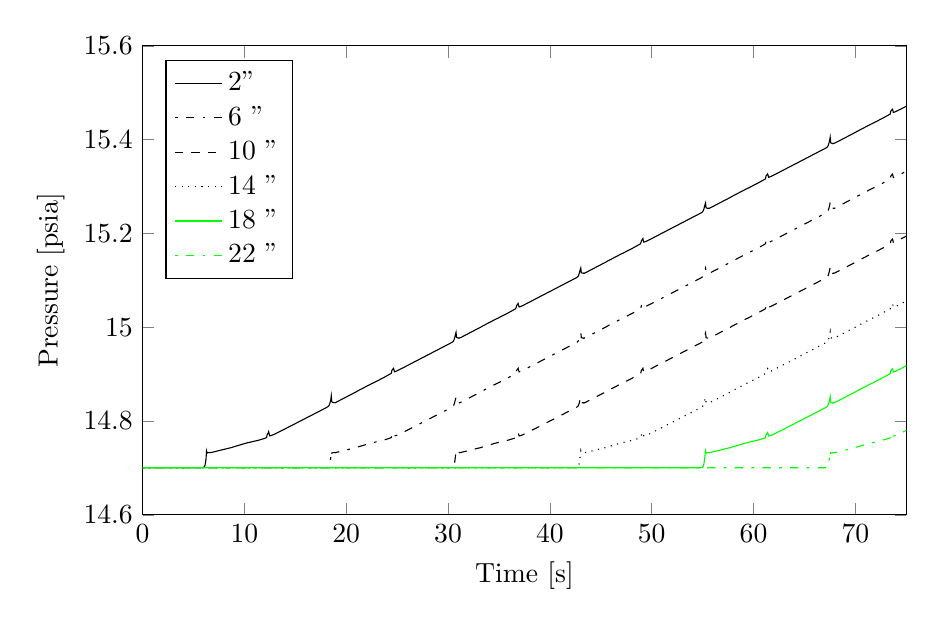
\begin{tikzpicture}

\begin{axis}[%
width=0.8\textwidth,
%height=0.630967741935484\textwidth,
height=0.491294629700995\textwidth,
scale only axis,
xmin=0,
xmax=75,
xlabel={Time [s]},
ymin=14.6,
ymax=15.6,
ylabel={Pressure [psia]},
legend style={at={(0.03,0.97)},anchor=north west,draw=black,fill=white,legend cell align=left}
]
\addplot [
color=black,
solid
]
table[row sep=crcr]{
0 14.7007818222046\\
9.99999971718069e-10 14.7007818222046\\
2.49999998480632e-09 14.7007818222046\\
4.74999994892755e-09 14.7007818222046\\
8.1250002281763e-09 14.7007818222046\\
1.31874999809156e-08 14.7007818222046\\
2.0781250498203e-08 14.7007818222046\\
3.21718758300449e-08 14.7007818222046\\
4.92578138278077e-08 14.7007818222046\\
7.48867208244519e-08 14.7007818222046\\
1.13330081319418e-07 14.7007818222046\\
1.70995122061868e-07 14.7007818222046\\
2.57492672517401e-07 14.7007818222046\\
3.8723902662241e-07 14.7007818222046\\
5.81858500936505e-07 14.7007818222046\\
8.73787769251066e-07 14.7007818222046\\
1.31168167172291e-06 14.7007818222046\\
1.9685226106958e-06 14.7007827758789\\
2.95378367809462e-06 14.7007827758789\\
4.43167573394021e-06 14.7007827758789\\
6.64851359033491e-06 14.7007827758789\\
9.97376992017962e-06 14.7007837295532\\
1.49616553244414e-05 14.7007846832275\\
2.24434825213393e-05 14.7007856369019\\
3.36662233166862e-05 14.7007865905762\\
5.05003372381907e-05 14.7007884979248\\
7.57515081204474e-05 14.7007904052734\\
0.000113628258986864 14.7007932662964\\
0.000170443381648511 14.700795173645\\
0.000255666091106832 14.7007970809937\\
0.000383500126190484 14.7007970809937\\
0.000575251178815961 14.7007942199707\\
0.000862877757754177 14.7007904052734\\
0.00129431765526533 14.7007865905762\\
0.00194147753063589 14.7007837295532\\
0.00291221728548408 14.700779914856\\
0.00436832662671804 14.7007780075073\\
0.00597004732117057 14.700779914856\\
0.00773194013163447 14.7007827758789\\
0.009670021943748 14.7007837295532\\
0.0118019115179777 14.7007837295532\\
0.0141469910740852 14.7007827758789\\
0.0167265776544809 14.7007827758789\\
0.0195641238242388 14.7007827758789\\
0.0226854234933853 14.7007827758789\\
0.0261188540607691 14.7007827758789\\
0.0298956278711557 14.7007827758789\\
0.0340500771999359 14.7007827758789\\
0.0386199727654457 14.7007827758789\\
0.0436468608677387 14.7007827758789\\
0.0491764321923256 14.7007827758789\\
0.0552589632570744 14.7007827758789\\
0.0619497485458851 14.7007827758789\\
0.0693096145987511 14.7007827758789\\
0.0774054601788521 14.7007827758789\\
0.0863108932971954 14.700779914856\\
0.0961068719625473 14.7007827758789\\
0.106882445514202 14.7007827758789\\
0.118735581636429 14.7007827758789\\
0.13177402317524 14.7007827758789\\
0.146116316318512 14.7007827758789\\
0.161892831325531 14.7007827758789\\
0.179247006773949 14.7007827758789\\
0.198336601257324 14.7007827758789\\
0.21933513879776 14.7007827758789\\
0.242433547973633 14.7007827758789\\
0.267841786146164 14.7007827758789\\
0.29579085111618 14.7007827758789\\
0.32653483748436 14.7007827758789\\
0.360353201627731 14.7007827758789\\
0.397553414106369 14.7007837295532\\
0.438473641872406 14.7007837295532\\
0.483485877513886 14.7007837295532\\
0.532999336719513 14.7007837295532\\
0.582999348640442 14.7007837295532\\
0.632999360561371 14.7007837295532\\
0.6829993724823 14.7007837295532\\
0.732999384403229 14.7007837295532\\
0.782999336719513 14.7007837295532\\
0.832999348640442 14.7007837295532\\
0.882999360561371 14.7007837295532\\
0.9329993724823 14.7007837295532\\
0.982999384403229 14.7007837295532\\
1.03299939632416 14.7007827758789\\
1.08299934864044 14.7007827758789\\
1.13299930095673 14.7007827758789\\
1.1829993724823 14.7007827758789\\
1.23299932479858 14.7007827758789\\
1.28299939632416 14.7007827758789\\
1.33299934864044 14.7007827758789\\
1.38299930095673 14.7007827758789\\
1.4329993724823 14.7007827758789\\
1.48299932479858 14.7007827758789\\
1.53299939632416 14.7007827758789\\
1.58299934864044 14.7007827758789\\
1.63299930095673 14.7007827758789\\
1.6829993724823 14.7007827758789\\
1.73299932479858 14.7007827758789\\
1.78299939632416 14.7007827758789\\
1.83299934864044 14.7007827758789\\
1.88299930095673 14.7007827758789\\
1.9329993724823 14.7007827758789\\
1.98299932479858 14.7007827758789\\
2.03299927711487 14.7007827758789\\
2.08299946784973 14.7007827758789\\
2.13299942016602 14.7007827758789\\
2.1829993724823 14.7007827758789\\
2.23299932479858 14.7007827758789\\
2.28299927711487 14.7007827758789\\
2.33299946784973 14.7007827758789\\
2.38299942016602 14.7007827758789\\
2.4329993724823 14.7007827758789\\
2.48299932479858 14.7007827758789\\
2.53299927711487 14.7007827758789\\
2.58299946784973 14.7007827758789\\
2.63299942016602 14.7007827758789\\
2.6829993724823 14.7007827758789\\
2.73299932479858 14.7007827758789\\
2.78299927711487 14.7007827758789\\
2.83299946784973 14.7007827758789\\
2.88299942016602 14.7007827758789\\
2.9329993724823 14.7007827758789\\
2.98299932479858 14.7007827758789\\
3.03299927711487 14.7007827758789\\
3.08299946784973 14.7007827758789\\
3.13299942016602 14.7007827758789\\
3.1829993724823 14.7007827758789\\
3.23299932479858 14.7007827758789\\
3.28299927711487 14.7007827758789\\
3.33299946784973 14.7007827758789\\
3.38299942016602 14.7007827758789\\
3.4329993724823 14.7007827758789\\
3.48299932479858 14.7007827758789\\
3.53299927711487 14.7007827758789\\
3.58299946784973 14.7007827758789\\
3.63299942016602 14.7007827758789\\
3.6829993724823 14.7007827758789\\
3.73299932479858 14.7007827758789\\
3.78299927711487 14.7007827758789\\
3.83299946784973 14.7007827758789\\
3.88299942016602 14.7007827758789\\
3.9329993724823 14.7007827758789\\
3.98299932479858 14.7007827758789\\
4.03299951553345 14.7007827758789\\
4.08299922943115 14.7007827758789\\
4.13299942016602 14.7007827758789\\
4.18299913406372 14.7007827758789\\
4.23299932479858 14.7007827758789\\
4.28299951553345 14.7007827758789\\
4.33299922943115 14.7007827758789\\
4.38299942016602 14.7007827758789\\
4.43299913406372 14.7007827758789\\
4.48299932479858 14.7007827758789\\
4.53299951553345 14.7007827758789\\
4.58299922943115 14.7007827758789\\
4.63299942016602 14.7007827758789\\
4.68299913406372 14.7007827758789\\
4.73299932479858 14.7007827758789\\
4.78299951553345 14.7007827758789\\
4.83299922943115 14.7007827758789\\
4.88299942016602 14.7007827758789\\
4.93299913406372 14.7007827758789\\
4.98299932479858 14.7007827758789\\
5.03299951553345 14.7007827758789\\
5.08299922943115 14.7007827758789\\
5.13299942016602 14.7007827758789\\
5.18299913406372 14.7007827758789\\
5.23299932479858 14.7007827758789\\
5.28299951553345 14.7007827758789\\
5.33299922943115 14.7007827758789\\
5.38299942016602 14.7007827758789\\
5.43299913406372 14.7007827758789\\
5.48299932479858 14.7007837295532\\
5.53299951553345 14.7007837295532\\
5.58299922943115 14.7007837295532\\
5.63299942016602 14.7007856369019\\
5.68299913406372 14.7007865905762\\
5.73299932479858 14.7007913589478\\
5.78299951553345 14.7008008956909\\
5.83299922943115 14.7008218765259\\
5.88299942016602 14.7008686065674\\
5.93299913406372 14.7009773254395\\
5.98299932479858 14.7012338638306\\
6.03299951553345 14.7018346786499\\
6.08299922943115 14.7031946182251\\
6.13299942016602 14.7060613632202\\
6.18299913406372 14.7113580703735\\
6.23299932479858 14.719313621521\\
6.28299951553345 14.7358856201172\\
6.33299922943115 14.7318172454834\\
6.38299942016602 14.7319145202637\\
6.43299913406372 14.732569694519\\
6.48299932479858 14.732780456543\\
6.53299951553345 14.7329292297363\\
6.58299922943115 14.7330045700073\\
6.63299942016602 14.7329235076904\\
6.68299913406372 14.7327470779419\\
6.73299932479858 14.7329006195068\\
6.78299951553345 14.7331695556641\\
6.83299922943115 14.7334308624268\\
6.88299942016602 14.7336978912354\\
6.93299913406372 14.7339630126953\\
6.98299932479858 14.7342290878296\\
7.03299951553345 14.7344942092896\\
7.08299922943115 14.7347593307495\\
7.13299942016602 14.7350244522095\\
7.18299913406372 14.7352905273438\\
7.23299932479858 14.7355556488037\\
7.28299951553345 14.7358207702637\\
7.33299922943115 14.7360868453979\\
7.38299942016602 14.7363519668579\\
7.43299913406372 14.7366180419922\\
7.48299932479858 14.7368831634521\\
7.53299951553345 14.7371482849121\\
7.58299922943115 14.7374143600464\\
7.63299942016602 14.7376794815063\\
7.68299913406372 14.7379455566406\\
7.73299932479858 14.7382106781006\\
7.78299951553345 14.7384767532349\\
7.83299922943115 14.7387418746948\\
7.88299942016602 14.7390079498291\\
7.93299913406372 14.7392730712891\\
7.98299932479858 14.7395391464233\\
8.03299903869629 14.7398052215576\\
8.08299922943115 14.7400703430176\\
8.13299942016602 14.7403364181519\\
8.18299961090088 14.7406024932861\\
8.23299980163574 14.7408676147461\\
8.28299903869629 14.7411336898804\\
8.33299922943115 14.7413997650146\\
8.38299942016602 14.7416658401489\\
8.43299961090088 14.7419319152832\\
8.48299980163574 14.7421979904175\\
8.53299903869629 14.7424640655518\\
8.58299922943115 14.742730140686\\
8.63299942016602 14.7429962158203\\
8.68299961090088 14.7432622909546\\
8.73299980163574 14.7435283660889\\
8.78299903869629 14.7437944412231\\
8.83299922943115 14.7442302703857\\
8.88299942016602 14.7446527481079\\
8.93299961090088 14.7449893951416\\
8.98299980163574 14.7453165054321\\
9.03299903869629 14.7456398010254\\
9.08299922943115 14.7459630966187\\
9.13299942016602 14.7462854385376\\
9.18299961090088 14.7466077804565\\
9.23299980163574 14.7469291687012\\
9.28299903869629 14.7472505569458\\
9.33299922943115 14.7475709915161\\
9.38299942016602 14.7478914260864\\
9.43299961090088 14.7482118606567\\
9.48299980163574 14.7485313415527\\
9.53299903869629 14.748851776123\\
9.58299922943115 14.749171257019\\
9.63299942016602 14.7494897842407\\
9.68299961090088 14.7498092651367\\
9.73299980163574 14.7501277923584\\
9.78299903869629 14.7504472732544\\
9.83299922943115 14.7507658004761\\
9.88299942016602 14.7510843276978\\
9.93299961090088 14.7514019012451\\
9.98299980163574 14.7517204284668\\
10.0329990386963 14.7520389556885\\
10.0829992294312 14.7523565292358\\
10.132999420166 14.7526750564575\\
10.1829996109009 14.7529935836792\\
10.2329998016357 14.7533111572266\\
10.2829990386963 14.7536182403564\\
10.3329992294312 14.7538833618164\\
10.382999420166 14.7539463043213\\
10.4329996109009 14.7542095184326\\
10.4829998016357 14.754469871521\\
10.5329990386963 14.7547359466553\\
10.5829992294312 14.7549991607666\\
10.632999420166 14.7552623748779\\
10.6829996109009 14.7555236816406\\
10.7329998016357 14.7557849884033\\
10.7829990386963 14.7560443878174\\
10.8329992294312 14.7563028335571\\
10.882999420166 14.7565603256226\\
10.9329996109009 14.7568159103394\\
10.9829998016357 14.7570695877075\\
11.0329990386963 14.7573223114014\\
11.0829992294312 14.7575740814209\\
11.132999420166 14.7578229904175\\
11.1829996109009 14.7580699920654\\
11.2329998016357 14.7583150863647\\
11.2829990386963 14.7585582733154\\
11.3329992294312 14.7587985992432\\
11.382999420166 14.7590579986572\\
11.4329996109009 14.7593879699707\\
11.4829998016357 14.7596836090088\\
11.5329990386963 14.7599534988403\\
11.5829992294312 14.7604160308838\\
11.632999420166 14.7607583999634\\
11.6829996109009 14.7610578536987\\
11.7329998016357 14.7613754272461\\
11.7829990386963 14.7616958618164\\
11.8329992294312 14.7620239257813\\
11.882999420166 14.7623605728149\\
11.9329996109009 14.7627077102661\\
11.9829998016357 14.7630672454834\\
12.0329990386963 14.7634429931641\\
12.0829992294312 14.7638387680054\\
12.132999420166 14.7642621994019\\
12.1829996109009 14.7651968002319\\
12.2329998016357 14.770655632019\\
12.2829990386963 14.772385597229\\
12.3329992294312 14.7741975784302\\
12.382999420166 14.7773275375366\\
12.4329996109009 14.7730026245117\\
12.4829998016357 14.7684373855591\\
12.5329990386963 14.7686653137207\\
12.5829992294312 14.7689294815063\\
12.632999420166 14.7692222595215\\
12.6829996109009 14.7695665359497\\
12.7329998016357 14.7699575424194\\
12.7829990386963 14.7703914642334\\
12.8329992294312 14.7708559036255\\
12.882999420166 14.7713422775269\\
12.9329996109009 14.771842956543\\
12.9829998016357 14.7723531723022\\
13.0329990386963 14.7728719711304\\
13.0829992294312 14.7733955383301\\
13.132999420166 14.7739248275757\\
13.1829996109009 14.7744579315186\\
13.2329998016357 14.7749967575073\\
13.2829990386963 14.7755346298218\\
13.3329992294312 14.7760763168335\\
13.382999420166 14.7766199111938\\
13.4329996109009 14.7771663665771\\
13.4829998016357 14.7777156829834\\
13.5329990386963 14.7782669067383\\
13.5829992294312 14.7788190841675\\
13.632999420166 14.779372215271\\
13.6829996109009 14.7799263000488\\
13.7329998016357 14.7804803848267\\
13.7829990386963 14.7810344696045\\
13.8329992294312 14.7815895080566\\
13.882999420166 14.7821435928345\\
13.9329996109009 14.7826976776123\\
13.9829998016357 14.7832527160645\\
14.0329990386963 14.7838068008423\\
14.0829992294312 14.7843618392944\\
14.132999420166 14.7849168777466\\
14.1829996109009 14.7854709625244\\
14.2329998016357 14.7860260009766\\
14.2829990386963 14.7865810394287\\
14.3329992294312 14.7871360778809\\
14.382999420166 14.787691116333\\
14.4329996109009 14.7882461547852\\
14.4829998016357 14.7888011932373\\
14.5329990386963 14.7893571853638\\
14.5829992294312 14.7899122238159\\
14.632999420166 14.7904682159424\\
14.6829996109009 14.7910232543945\\
14.7329998016357 14.791579246521\\
14.7829990386963 14.7921342849731\\
14.8329992294312 14.7926902770996\\
14.882999420166 14.7932462692261\\
14.9329996109009 14.7938022613525\\
14.9829998016357 14.794358253479\\
15.0329990386963 14.7949151992798\\
15.0829992294312 14.7954711914063\\
15.132999420166 14.7960271835327\\
15.1829996109009 14.7965841293335\\
15.2329998016357 14.79714012146\\
15.2829990386963 14.7976970672607\\
15.3329992294312 14.7982654571533\\
15.382999420166 14.7988080978394\\
15.4329996109009 14.7993659973145\\
15.4829998016357 14.7999248504639\\
15.5329990386963 14.8004846572876\\
15.5829992294312 14.801043510437\\
15.632999420166 14.8016033172607\\
15.6829996109009 14.8021631240845\\
15.7329998016357 14.8027229309082\\
15.7829990386963 14.8032817840576\\
15.8329992294312 14.8038415908813\\
15.882999420166 14.8044013977051\\
15.9329996109009 14.8049612045288\\
15.9829998016357 14.8055210113525\\
16.0329990386963 14.8060808181763\\
16.0830001831055 14.806640625\\
16.132999420166 14.8072004318237\\
16.1829986572266 14.8077611923218\\
16.2329998016357 14.8083209991455\\
16.2829990386963 14.8088808059692\\
16.3330001831055 14.809440612793\\
16.382999420166 14.810001373291\\
16.4329986572266 14.8105611801147\\
16.4829998016357 14.8111219406128\\
16.5329990386963 14.8116817474365\\
16.5830001831055 14.8122425079346\\
16.632999420166 14.8128023147583\\
16.6829986572266 14.8133630752563\\
16.7329998016357 14.8139228820801\\
16.7829990386963 14.8144836425781\\
16.8330001831055 14.8150444030762\\
16.882999420166 14.8156051635742\\
16.9329986572266 14.8161659240723\\
16.9829998016357 14.816725730896\\
17.0329990386963 14.817286491394\\
17.0830001831055 14.8178472518921\\
17.132999420166 14.8184080123901\\
17.1829986572266 14.8189687728882\\
17.2329998016357 14.8195304870605\\
17.2829990386963 14.8200912475586\\
17.3330001831055 14.8206520080566\\
17.382999420166 14.8212127685547\\
17.4329986572266 14.8217744827271\\
17.4829998016357 14.8223352432251\\
17.5329990386963 14.8228960037231\\
17.5830001831055 14.8234577178955\\
17.632999420166 14.8240184783936\\
17.6829986572266 14.8245801925659\\
17.7329998016357 14.825140953064\\
17.7829990386963 14.8257026672363\\
17.8330001831055 14.8262643814087\\
17.882999420166 14.8268270492554\\
17.9329986572266 14.8273887634277\\
17.9829998016357 14.8279552459717\\
18.0329990386963 14.8285255432129\\
18.0830001831055 14.8291053771973\\
18.132999420166 14.8297109603882\\
18.1829986572266 14.830376625061\\
18.2329998016357 14.8311824798584\\
18.2829990386963 14.8323011398315\\
18.3330001831055 14.8340578079224\\
18.382999420166 14.836895942688\\
18.4329986572266 14.8409700393677\\
18.4829998016357 14.8454065322876\\
18.5329990386963 14.8538360595703\\
18.5830001831055 14.841178894043\\
18.632999420166 14.8400831222534\\
18.6829986572266 14.8397035598755\\
18.7329998016357 14.8393955230713\\
18.7829990386963 14.8392553329468\\
18.8330001831055 14.8391199111938\\
18.882999420166 14.8394784927368\\
18.9329986572266 14.8391151428223\\
18.9829998016357 14.8396854400635\\
19.0329990386963 14.8404207229614\\
19.0830001831055 14.8410863876343\\
19.132999420166 14.8414373397827\\
19.1829986572266 14.8420810699463\\
19.2329998016357 14.842604637146\\
19.2829990386963 14.8431854248047\\
19.3330001831055 14.8437395095825\\
19.382999420166 14.8443059921265\\
19.4329986572266 14.8448667526245\\
19.4829998016357 14.8454313278198\\
19.5329990386963 14.8459930419922\\
19.5830001831055 14.8465566635132\\
19.632999420166 14.8471193313599\\
19.6829986572266 14.8476819992065\\
19.7329998016357 14.8482446670532\\
19.7829990386963 14.8488082885742\\
19.8330001831055 14.8493709564209\\
19.882999420166 14.8499336242676\\
19.9329986572266 14.8504972457886\\
19.9829998016357 14.8510599136353\\
20.0329990386963 14.8516235351563\\
20.0830001831055 14.8521862030029\\
20.132999420166 14.8527498245239\\
20.1829986572266 14.8533124923706\\
20.2329998016357 14.8538761138916\\
20.2829990386963 14.8544387817383\\
20.3330001831055 14.8550024032593\\
20.382999420166 14.8555660247803\\
20.4329986572266 14.8561296463013\\
20.4829998016357 14.8566923141479\\
20.5329990386963 14.8572559356689\\
20.5830001831055 14.8578195571899\\
20.632999420166 14.8583831787109\\
20.6829986572266 14.8589468002319\\
20.7329998016357 14.8595104217529\\
20.7829990386963 14.8600740432739\\
20.8330001831055 14.8606376647949\\
20.882999420166 14.8612012863159\\
20.9329986572266 14.8617649078369\\
20.9829998016357 14.8623285293579\\
21.0329990386963 14.8628921508789\\
21.0830001831055 14.8636484146118\\
21.132999420166 14.8643102645874\\
21.1829986572266 14.8648853302002\\
21.2329998016357 14.8654527664185\\
21.2829990386963 14.8660163879395\\
21.3330001831055 14.8665809631348\\
21.382999420166 14.8671455383301\\
21.4329986572266 14.8677091598511\\
21.4829998016357 14.8682737350464\\
21.5329990386963 14.8688383102417\\
21.5830001831055 14.869402885437\\
21.632999420166 14.8699674606323\\
21.6829986572266 14.8705320358276\\
21.7329998016357 14.8710966110229\\
21.7829990386963 14.8716621398926\\
21.8330001831055 14.8722267150879\\
21.882999420166 14.8727922439575\\
21.9329986572266 14.8733577728271\\
21.9829998016357 14.8739223480225\\
22.0329990386963 14.8744878768921\\
22.0830001831055 14.875054359436\\
22.132999420166 14.8756198883057\\
22.1829986572266 14.8761854171753\\
22.2329998016357 14.8767518997192\\
22.2829990386963 14.8773174285889\\
22.3330001831055 14.8778839111328\\
22.382999420166 14.8784503936768\\
22.4329986572266 14.8790168762207\\
22.4829998016357 14.8795833587646\\
22.5329990386963 14.8801431655884\\
22.5830001831055 14.8806686401367\\
22.632999420166 14.8809804916382\\
22.6829986572266 14.8815402984619\\
22.7329998016357 14.8820934295654\\
22.7829990386963 14.8826551437378\\
22.8330001831055 14.8832149505615\\
22.882999420166 14.8837747573853\\
22.9329986572266 14.8843336105347\\
22.9829998016357 14.8848934173584\\
23.0329990386963 14.8854522705078\\
23.0830001831055 14.8860111236572\\
23.132999420166 14.8865690231323\\
23.1829986572266 14.8871269226074\\
23.2329998016357 14.8876848220825\\
23.2829990386963 14.8882427215576\\
23.3330001831055 14.8887996673584\\
23.382999420166 14.8893566131592\\
23.4329986572266 14.8899126052856\\
23.4829998016357 14.8904685974121\\
23.5329990386963 14.8910245895386\\
23.5830001831055 14.8915796279907\\
23.632999420166 14.8921527862549\\
23.6829986572266 14.8927812576294\\
23.7329998016357 14.8933725357056\\
23.7829990386963 14.8939409255981\\
23.8330001831055 14.8946504592896\\
23.882999420166 14.8952522277832\\
23.9329986572266 14.8958168029785\\
23.9829998016357 14.8963966369629\\
24.0329990386963 14.8969774246216\\
24.0830001831055 14.8975639343262\\
24.132999420166 14.8981552124023\\
24.1829986572266 14.8987531661987\\
24.2329998016357 14.8993587493896\\
24.2829990386963 14.899974822998\\
24.3330001831055 14.9006052017212\\
24.382999420166 14.901252746582\\
24.4329986572266 14.9022483825684\\
24.4829998016357 14.9080715179443\\
24.5329990386963 14.909327507019\\
24.5830001831055 14.9107666015625\\
24.632999420166 14.9123458862305\\
24.6829986572266 14.9096565246582\\
24.7329998016357 14.9049825668335\\
24.7829990386963 14.9054279327393\\
24.8330001831055 14.9057788848877\\
24.882999420166 14.9061832427979\\
24.9329986572266 14.9066190719604\\
24.9829998016357 14.9070892333984\\
25.0329990386963 14.9075908660889\\
25.0830001831055 14.9081144332886\\
25.132999420166 14.9086513519287\\
25.1829986572266 14.9091949462891\\
25.2329998016357 14.909743309021\\
25.2829990386963 14.9102945327759\\
25.3330001831055 14.9108476638794\\
25.382999420166 14.9114017486572\\
25.4329986572266 14.9119567871094\\
25.4829998016357 14.9125137329102\\
25.5329990386963 14.9130725860596\\
25.5830001831055 14.9136304855347\\
25.632999420166 14.9141874313354\\
25.6829986572266 14.9147453308105\\
25.7329998016357 14.91530418396\\
25.7829990386963 14.9158639907837\\
25.8330001831055 14.9164247512817\\
25.882999420166 14.9169855117798\\
25.9329986572266 14.9175481796265\\
25.9829998016357 14.9181108474731\\
26.0329990386963 14.9186744689941\\
26.0830001831055 14.9192390441895\\
26.132999420166 14.9198026657104\\
26.1829986572266 14.9203662872314\\
26.2329998016357 14.9209299087524\\
26.2829990386963 14.9214944839478\\
26.3330001831055 14.9220581054688\\
26.382999420166 14.9226226806641\\
26.4329986572266 14.9231863021851\\
26.4829998016357 14.9237499237061\\
26.5329990386963 14.9243144989014\\
26.5830001831055 14.9248781204224\\
26.632999420166 14.9254417419434\\
26.6829986572266 14.9260063171387\\
26.7329998016357 14.9265699386597\\
26.7829990386963 14.9271335601807\\
26.8330001831055 14.927698135376\\
26.882999420166 14.928261756897\\
26.9329986572266 14.928825378418\\
26.9829998016357 14.9293899536133\\
27.0329990386963 14.9299535751343\\
27.0830001831055 14.9305171966553\\
27.132999420166 14.9310817718506\\
27.1829986572266 14.9316453933716\\
27.2329998016357 14.9322090148926\\
27.2829990386963 14.9327735900879\\
27.3330001831055 14.9333372116089\\
27.382999420166 14.9339008331299\\
27.4329986572266 14.9344654083252\\
27.4829998016357 14.9350290298462\\
27.5329990386963 14.9355926513672\\
27.5830001831055 14.9361572265625\\
27.632999420166 14.9367208480835\\
27.6829986572266 14.9372844696045\\
27.7329998016357 14.9378490447998\\
27.7829990386963 14.9384126663208\\
27.8330001831055 14.9389762878418\\
27.882999420166 14.9395399093628\\
27.9329986572266 14.9401044845581\\
27.9829998016357 14.9406681060791\\
28.0329990386963 14.9412317276001\\
28.0830001831055 14.9417963027954\\
28.132999420166 14.9423599243164\\
28.1829986572266 14.9429378509521\\
28.2329998016357 14.9434814453125\\
28.2829990386963 14.9440441131592\\
28.3330001831055 14.9446077346802\\
28.382999420166 14.9451723098755\\
28.4329986572266 14.9457359313965\\
28.4829998016357 14.9462995529175\\
28.5329990386963 14.9468641281128\\
28.5830001831055 14.9474277496338\\
28.632999420166 14.9479923248291\\
28.6829986572266 14.9485559463501\\
28.7329998016357 14.9491195678711\\
28.7829990386963 14.9496841430664\\
28.8330001831055 14.9502477645874\\
28.882999420166 14.9508123397827\\
28.9329986572266 14.9513759613037\\
28.9829998016357 14.9519395828247\\
29.0329990386963 14.95250415802\\
29.0830001831055 14.953067779541\\
29.132999420166 14.9536323547363\\
29.1829986572266 14.9541959762573\\
29.2329998016357 14.9547595977783\\
29.2829990386963 14.9553241729736\\
29.3330001831055 14.9558877944946\\
29.382999420166 14.9564523696899\\
29.4329986572266 14.9570159912109\\
29.4829998016357 14.9575796127319\\
29.5329990386963 14.9581441879272\\
29.5830001831055 14.9587078094482\\
29.632999420166 14.9592723846436\\
29.6829986572266 14.9598360061646\\
29.7329998016357 14.9604005813599\\
29.7829990386963 14.9609642028809\\
29.8330001831055 14.9615278244019\\
29.882999420166 14.9620923995972\\
29.9329986572266 14.9626560211182\\
29.9829998016357 14.9632205963135\\
30.0329990386963 14.9637851715088\\
30.0830001831055 14.9643497467041\\
30.132999420166 14.9649152755737\\
30.1829986572266 14.965479850769\\
30.2329998016357 14.9660501480103\\
30.2829990386963 14.9666261672974\\
30.3330001831055 14.9672174453735\\
30.382999420166 14.9678449630737\\
30.4329986572266 14.9685583114624\\
30.4829998016357 14.9694700241089\\
30.5329990386963 14.9708194732666\\
30.5830001831055 14.9729900360107\\
30.632999420166 14.9763927459717\\
30.6829986572266 14.9808139801025\\
30.7329998016357 14.9848794937134\\
30.7829990386963 14.9890556335449\\
30.8330001831055 14.9784059524536\\
30.882999420166 14.9777975082397\\
30.9329986572266 14.9774398803711\\
30.9829998016357 14.977201461792\\
31.0329990386963 14.9767684936523\\
31.0830001831055 14.9774942398071\\
31.132999420166 14.9769878387451\\
31.1829986572266 14.9775276184082\\
31.2329998016357 14.9778909683228\\
31.2829990386963 14.9785318374634\\
31.3330001831055 14.9790601730347\\
31.382999420166 14.9796419143677\\
31.4329986572266 14.9801979064941\\
31.4829998016357 14.9807653427124\\
31.5329990386963 14.9813280105591\\
31.5830001831055 14.9818935394287\\
31.632999420166 14.9824571609497\\
31.6829986572266 14.983021736145\\
31.7329998016357 14.983585357666\\
31.7829990386963 14.9841499328613\\
31.8330001831055 14.9847145080566\\
31.882999420166 14.9852781295776\\
31.9329986572266 14.9858427047729\\
31.9829998016357 14.9864072799683\\
32.0330009460449 14.9869709014893\\
32.0830001831055 14.9875354766846\\
32.132999420166 14.9881000518799\\
32.1829986572266 14.9886646270752\\
32.2329978942871 14.9892292022705\\
32.2830009460449 14.9897928237915\\
32.3330001831055 14.9903573989868\\
32.382999420166 14.9909219741821\\
32.4329986572266 14.9914855957031\\
32.4829978942871 14.9920501708984\\
32.5330009460449 14.9926147460938\\
32.5830001831055 14.9931793212891\\
32.632999420166 14.9937438964844\\
32.6829986572266 14.9943084716797\\
32.7329978942871 14.994873046875\\
32.7830009460449 14.9954376220703\\
32.8330001831055 14.9960021972656\\
32.882999420166 14.9965667724609\\
32.9329986572266 14.9971313476563\\
32.9829978942871 14.9976959228516\\
33.0330009460449 14.9982604980469\\
33.0830001831055 14.9988250732422\\
33.132999420166 14.9993896484375\\
33.1829986572266 14.9999542236328\\
33.2329978942871 15.0005187988281\\
33.2830009460449 15.0011043548584\\
33.3330001831055 15.001932144165\\
33.382999420166 15.0025043487549\\
33.4329986572266 15.0030794143677\\
33.4829978942871 15.0036430358887\\
33.5330009460449 15.0042085647583\\
33.5830001831055 15.0047731399536\\
33.632999420166 15.0053386688232\\
33.6829986572266 15.0059032440186\\
33.7329978942871 15.0064687728882\\
33.7830009460449 15.0070333480835\\
33.8330001831055 15.0075988769531\\
33.882999420166 15.0081644058228\\
33.9329986572266 15.0087299346924\\
33.9829978942871 15.009295463562\\
34.0330009460449 15.0098609924316\\
34.0830001831055 15.0104265213013\\
34.132999420166 15.0109930038452\\
34.1829986572266 15.0115585327148\\
34.2329978942871 15.0121250152588\\
34.2830009460449 15.0126905441284\\
34.3330001831055 15.0132570266724\\
34.382999420166 15.0138235092163\\
34.4329986572266 15.0143899917603\\
34.4829978942871 15.0149564743042\\
34.5330009460449 15.0155229568481\\
34.5830001831055 15.0160894393921\\
34.632999420166 15.0166568756104\\
34.6829986572266 15.0172233581543\\
34.7329978942871 15.0177907943726\\
34.7830009460449 15.0183401107788\\
34.8330001831055 15.0188236236572\\
34.882999420166 15.0191688537598\\
34.9329986572266 15.01975440979\\
34.9829978942871 15.0203056335449\\
35.0330009460449 15.0208692550659\\
35.0830001831055 15.0214281082153\\
35.132999420166 15.0219888687134\\
35.1829986572266 15.0225486755371\\
35.2329978942871 15.0231084823608\\
35.2830009460449 15.0236682891846\\
35.3330001831055 15.0242280960083\\
35.382999420166 15.0247869491577\\
35.4329986572266 15.0253458023071\\
35.4829978942871 15.0259046554565\\
35.5330009460449 15.0264625549316\\
35.5830001831055 15.0270204544067\\
35.632999420166 15.0275783538818\\
35.6829986572266 15.0281352996826\\
35.7329978942871 15.0286922454834\\
35.7830009460449 15.0292491912842\\
35.8330001831055 15.0298051834106\\
35.882999420166 15.0303964614868\\
35.9329986572266 15.0310096740723\\
35.9829978942871 15.0315914154053\\
36.0330009460449 15.0321598052979\\
36.0830001831055 15.0328788757324\\
36.132999420166 15.0334663391113\\
36.1829986572266 15.0340223312378\\
36.2329978942871 15.0346012115479\\
36.2830009460449 15.0351829528809\\
36.3330001831055 15.0357704162598\\
36.382999420166 15.0363626480103\\
36.4329986572266 15.036961555481\\
36.4829978942871 15.0375690460205\\
36.5330009460449 15.0381870269775\\
36.5830001831055 15.0388202667236\\
36.632999420166 15.0394716262817\\
36.6829986572266 15.0416326522827\\
36.7329978942871 15.0463647842407\\
36.7830009460449 15.0476837158203\\
36.8330001831055 15.0491361618042\\
36.882999420166 15.0507764816284\\
36.9329986572266 15.0458250045776\\
36.9829978942871 15.0431499481201\\
37.0330009460449 15.0435962677002\\
37.0830001831055 15.0439472198486\\
37.132999420166 15.0443706512451\\
37.1829986572266 15.0448122024536\\
37.2329978942871 15.0452919006348\\
37.2830009460449 15.0457992553711\\
37.3330001831055 15.0463266372681\\
37.382999420166 15.0468654632568\\
37.4329986572266 15.0474109649658\\
37.4829978942871 15.0479602813721\\
37.5330009460449 15.048511505127\\
37.5830001831055 15.0490646362305\\
37.632999420166 15.0496187210083\\
37.6829986572266 15.0501747131348\\
37.7329978942871 15.0507316589355\\
37.7830009460449 15.0512914657593\\
37.8330001831055 15.0518493652344\\
37.882999420166 15.0524063110352\\
37.9329986572266 15.0529651641846\\
37.9829978942871 15.053524017334\\
38.0330009460449 15.0540838241577\\
38.0830001831055 15.0546445846558\\
38.132999420166 15.0552053451538\\
38.1829986572266 15.0557680130005\\
38.2329978942871 15.0563306808472\\
38.2830009460449 15.0568943023682\\
38.3330001831055 15.0574579238892\\
38.382999420166 15.0580224990845\\
38.4329986572266 15.0585861206055\\
38.4829978942871 15.0591506958008\\
38.5330009460449 15.0597143173218\\
38.5830001831055 15.0602788925171\\
38.632999420166 15.0608425140381\\
38.6829986572266 15.0614070892334\\
38.7329978942871 15.0619707107544\\
38.7830009460449 15.0625352859497\\
38.8330001831055 15.063099861145\\
38.882999420166 15.063663482666\\
38.9329986572266 15.0642280578613\\
38.9829978942871 15.0647916793823\\
39.0330009460449 15.0653562545776\\
39.0830001831055 15.0659198760986\\
39.132999420166 15.0664844512939\\
39.1829986572266 15.0670480728149\\
39.2329978942871 15.0676126480103\\
39.2830009460449 15.0681762695313\\
39.3330001831055 15.0687408447266\\
39.382999420166 15.0693044662476\\
39.4329986572266 15.0698680877686\\
39.4829978942871 15.0704326629639\\
39.5330009460449 15.0709962844849\\
39.5830001831055 15.0715608596802\\
39.632999420166 15.0721244812012\\
39.6829986572266 15.0726890563965\\
39.7329978942871 15.0732526779175\\
39.7830009460449 15.0738172531128\\
39.8330001831055 15.0743808746338\\
39.882999420166 15.0749454498291\\
39.9329986572266 15.0755090713501\\
39.9829978942871 15.0760736465454\\
40.0330009460449 15.0766372680664\\
40.0830001831055 15.0772008895874\\
40.132999420166 15.0777654647827\\
40.1829986572266 15.0783290863037\\
40.2329978942871 15.078893661499\\
40.2830009460449 15.07945728302\\
40.3330001831055 15.0800218582153\\
40.382999420166 15.0805854797363\\
40.4329986572266 15.0811500549316\\
40.4829978942871 15.0817136764526\\
40.5330009460449 15.0822782516479\\
40.5830001831055 15.0828418731689\\
40.632999420166 15.0834054946899\\
40.6829986572266 15.0839700698853\\
40.7329978942871 15.0845336914063\\
40.7830009460449 15.085111618042\\
40.8330001831055 15.0856561660767\\
40.882999420166 15.0862188339233\\
40.9329986572266 15.0867824554443\\
40.9829978942871 15.0873470306396\\
41.0330009460449 15.0879106521606\\
41.0830001831055 15.088475227356\\
41.132999420166 15.089038848877\\
41.1829986572266 15.0896034240723\\
41.2329978942871 15.0901670455933\\
41.2830009460449 15.0907316207886\\
41.3330001831055 15.0912952423096\\
41.382999420166 15.0918598175049\\
41.4329986572266 15.0924243927002\\
41.4829978942871 15.0929880142212\\
41.5330009460449 15.0935525894165\\
41.5830001831055 15.0941162109375\\
41.632999420166 15.0946807861328\\
41.6829986572266 15.0952444076538\\
41.7329978942871 15.0958089828491\\
41.7830009460449 15.0963726043701\\
41.8330001831055 15.0969371795654\\
41.882999420166 15.0975008010864\\
41.9329986572266 15.0980653762817\\
41.9829978942871 15.0986289978027\\
42.0330009460449 15.099193572998\\
42.0830001831055 15.099757194519\\
42.132999420166 15.1003217697144\\
42.1829986572266 15.1008863449097\\
42.2329978942871 15.1014499664307\\
42.2830009460449 15.102014541626\\
42.3330001831055 15.1025791168213\\
42.382999420166 15.1031446456909\\
42.4329986572266 15.1037101745605\\
42.4829978942871 15.1042814254761\\
42.5330009460449 15.1048583984375\\
42.5830001831055 15.1054515838623\\
42.632999420166 15.1060857772827\\
42.6829986572266 15.1068124771118\\
42.7329978942871 15.1077547073364\\
42.7830009460449 15.1091680526733\\
42.8330001831055 15.1114482879639\\
42.882999420166 15.1149787902832\\
42.9329986572266 15.1194429397583\\
42.9829978942871 15.1233673095703\\
43.0330009460449 15.1265230178833\\
43.0830001831055 15.1164398193359\\
43.132999420166 15.1159381866455\\
43.1829986572266 15.1155824661255\\
43.2329978942871 15.1153631210327\\
43.2830009460449 15.1150007247925\\
43.3330001831055 15.1156139373779\\
43.382999420166 15.1151533126831\\
43.4329986572266 15.1157827377319\\
43.4829978942871 15.116114616394\\
43.5330009460449 15.1167697906494\\
43.5830001831055 15.1172914505005\\
43.632999420166 15.1178760528564\\
43.6829986572266 15.1184310913086\\
43.7329978942871 15.1189994812012\\
43.7830009460449 15.1195611953735\\
43.8330001831055 15.1201267242432\\
43.882999420166 15.1206903457642\\
43.9329986572266 15.1212549209595\\
43.9829978942871 15.1218194961548\\
44.0330009460449 15.1223840713501\\
44.0830001831055 15.1229486465454\\
44.132999420166 15.1235122680664\\
44.1829986572266 15.1240768432617\\
44.2329978942871 15.124641418457\\
44.2830009460449 15.1252059936523\\
44.3330001831055 15.1257705688477\\
44.382999420166 15.126335144043\\
44.4329986572266 15.126898765564\\
44.4829978942871 15.1274633407593\\
44.5330009460449 15.1280279159546\\
44.5830001831055 15.1285924911499\\
44.632999420166 15.1291570663452\\
44.6829986572266 15.1297216415405\\
44.7329978942871 15.1302862167358\\
44.7830009460449 15.1308507919312\\
44.8330001831055 15.1314153671265\\
44.882999420166 15.1319799423218\\
44.9329986572266 15.1325445175171\\
44.9829978942871 15.1331090927124\\
45.0330009460449 15.1336736679077\\
45.0830001831055 15.134238243103\\
45.132999420166 15.1348028182983\\
45.1829986572266 15.1353673934937\\
45.2329978942871 15.135931968689\\
45.2830009460449 15.1364965438843\\
45.3330001831055 15.1370611190796\\
45.382999420166 15.1376256942749\\
45.4329986572266 15.1381912231445\\
45.4829978942871 15.1387557983398\\
45.5330009460449 15.1393613815308\\
45.5830001831055 15.1401691436768\\
45.632999420166 15.1407403945923\\
45.6829986572266 15.1413145065308\\
45.7329978942871 15.1418790817261\\
45.7830009460449 15.1424436569214\\
45.8330001831055 15.143009185791\\
45.882999420166 15.1435737609863\\
45.9329986572266 15.144139289856\\
45.9829978942871 15.1447048187256\\
46.0330009460449 15.1452703475952\\
46.0830001831055 15.1458358764648\\
46.132999420166 15.1464014053345\\
46.1829986572266 15.1469669342041\\
46.2329978942871 15.1475324630737\\
46.2830009460449 15.1480979919434\\
46.3330001831055 15.148663520813\\
46.382999420166 15.1492300033569\\
46.4329986572266 15.1497955322266\\
46.4829978942871 15.1503620147705\\
46.5330009460449 15.1509284973145\\
46.5830001831055 15.1514940261841\\
46.632999420166 15.152060508728\\
46.6829986572266 15.152626991272\\
46.7329978942871 15.1531944274902\\
46.7830009460449 15.1537609100342\\
46.8330001831055 15.1543273925781\\
46.882999420166 15.1548948287964\\
46.9329986572266 15.1554622650146\\
46.9829978942871 15.1560297012329\\
47.0330009460449 15.1565780639648\\
47.0830001831055 15.1570491790771\\
47.132999420166 15.1574115753174\\
47.1829986572266 15.1579942703247\\
47.2329978942871 15.1585474014282\\
47.2830009460449 15.1591100692749\\
47.3330001831055 15.1596698760986\\
47.382999420166 15.1602306365967\\
47.4329986572266 15.1607913970947\\
47.4829978942871 15.1613512039185\\
47.5330009460449 15.1619110107422\\
47.5830001831055 15.1624708175659\\
47.632999420166 15.1630306243896\\
47.6829986572266 15.1635894775391\\
47.7329978942871 15.1641483306885\\
47.7830009460449 15.1647071838379\\
47.8330001831055 15.1652660369873\\
47.882999420166 15.1658239364624\\
47.9329986572266 15.1663818359375\\
47.9829978942871 15.1669387817383\\
48.0330009460449 15.1674957275391\\
48.0830001831055 15.1680526733398\\
48.132999420166 15.1686458587646\\
48.1829986572266 15.1692543029785\\
48.2329978942871 15.1698341369629\\
48.2830009460449 15.1704025268555\\
48.3330001831055 15.1711149215698\\
48.382999420166 15.1716995239258\\
48.4329986572266 15.1722555160522\\
48.4829978942871 15.1728343963623\\
48.5330009460449 15.1734161376953\\
48.5830001831055 15.1740036010742\\
48.632999420166 15.1745958328247\\
48.6829986572266 15.1751947402954\\
48.7329978942871 15.175802230835\\
48.7830009460449 15.176420211792\\
48.8330001831055 15.1770534515381\\
48.882999420166 15.1777048110962\\
48.9329986572266 15.1800498962402\\
48.9829978942871 15.184609413147\\
49.0330009460449 15.1859378814697\\
49.0830001831055 15.1873912811279\\
49.132999420166 15.1890392303467\\
49.1829986572266 15.1836700439453\\
49.2329978942871 15.1813821792603\\
49.2830009460449 15.1818265914917\\
49.3330001831055 15.1821813583374\\
49.382999420166 15.1826047897339\\
49.4329986572266 15.183048248291\\
49.4829978942871 15.1835289001465\\
49.5330009460449 15.1840381622314\\
49.5830001831055 15.1845664978027\\
49.632999420166 15.1851053237915\\
49.6829986572266 15.1856508255005\\
49.7329978942871 15.1862001419067\\
49.7830009460449 15.1867513656616\\
49.8330001831055 15.1873044967651\\
49.882999420166 15.1878595352173\\
49.9329986572266 15.1884155273438\\
49.9829978942871 15.1889724731445\\
50.0330009460449 15.1895313262939\\
50.0830001831055 15.1900901794434\\
50.132999420166 15.1906480789185\\
50.1829986572266 15.1912059783936\\
50.2329978942871 15.191764831543\\
50.2830009460449 15.1923246383667\\
50.3330001831055 15.1928863525391\\
50.382999420166 15.1934471130371\\
50.4329986572266 15.1940088272095\\
50.4829978942871 15.1945714950562\\
50.5330009460449 15.1951351165771\\
50.5830001831055 15.1956996917725\\
50.632999420166 15.1962633132935\\
50.6829986572266 15.1968278884888\\
50.7329978942871 15.1973915100098\\
50.7830009460449 15.1979560852051\\
50.8330001831055 15.1985197067261\\
50.882999420166 15.1990842819214\\
50.9329986572266 15.1996479034424\\
50.9829978942871 15.2002124786377\\
51.0330009460449 15.200777053833\\
51.0830001831055 15.201340675354\\
51.132999420166 15.2019052505493\\
51.1829986572266 15.2024688720703\\
51.2329978942871 15.2030334472656\\
51.2830009460449 15.2035970687866\\
51.3330001831055 15.2041616439819\\
51.382999420166 15.2047262191772\\
51.4329986572266 15.2052898406982\\
51.4829978942871 15.2058544158936\\
51.5330009460449 15.2064180374146\\
51.5830001831055 15.2069826126099\\
51.632999420166 15.2075462341309\\
51.6829986572266 15.2081108093262\\
51.7329978942871 15.2086744308472\\
51.7830009460449 15.2092390060425\\
51.8330001831055 15.2098026275635\\
51.882999420166 15.2103672027588\\
51.9329986572266 15.2109308242798\\
51.9829978942871 15.2114953994751\\
52.0330009460449 15.2120590209961\\
52.0830001831055 15.2126235961914\\
52.132999420166 15.2131872177124\\
52.1829986572266 15.2137517929077\\
52.2329978942871 15.2143154144287\\
52.2830009460449 15.214879989624\\
52.3330001831055 15.215443611145\\
52.382999420166 15.2160081863403\\
52.4329986572266 15.2165718078613\\
52.4829978942871 15.2171363830566\\
52.5330009460449 15.2177000045776\\
52.5830001831055 15.2182645797729\\
52.632999420166 15.2188282012939\\
52.6829986572266 15.2193927764893\\
52.7329978942871 15.2199563980103\\
52.7830009460449 15.2205209732056\\
52.8330001831055 15.2210845947266\\
52.882999420166 15.2216491699219\\
52.9329986572266 15.2222127914429\\
52.9829978942871 15.2227773666382\\
53.0330009460449 15.2233409881592\\
53.0830001831055 15.2239055633545\\
53.132999420166 15.2244691848755\\
53.1829986572266 15.2250337600708\\
53.2329978942871 15.2256116867065\\
53.2830009460449 15.2261562347412\\
53.3330001831055 15.2267189025879\\
53.382999420166 15.2272825241089\\
53.4329986572266 15.2278470993042\\
53.4829978942871 15.2284107208252\\
53.5330009460449 15.2289752960205\\
53.5830001831055 15.2295398712158\\
53.632999420166 15.2301034927368\\
53.6829986572266 15.2306680679321\\
53.7329978942871 15.2312316894531\\
53.7830009460449 15.2317962646484\\
53.8330001831055 15.2323598861694\\
53.882999420166 15.2329244613647\\
53.9329986572266 15.2334880828857\\
53.9829978942871 15.2340526580811\\
54.0330009460449 15.2346172332764\\
54.0830001831055 15.2351808547974\\
54.132999420166 15.2357454299927\\
54.1829986572266 15.2363090515137\\
54.2329978942871 15.236873626709\\
54.2830009460449 15.23743724823\\
54.3330001831055 15.2380018234253\\
54.382999420166 15.2385663986206\\
54.4329986572266 15.2391300201416\\
54.4829978942871 15.2396945953369\\
54.5330009460449 15.2402591705322\\
54.5830001831055 15.2408237457275\\
54.632999420166 15.2413892745972\\
54.6829986572266 15.2419548034668\\
54.7329978942871 15.2425260543823\\
54.7830009460449 15.2431030273438\\
54.8330001831055 15.2436962127686\\
54.882999420166 15.2443294525146\\
54.9329986572266 15.2450561523438\\
54.9829978942871 15.2459955215454\\
55.0330009460449 15.2474031448364\\
55.0830001831055 15.2496757507324\\
55.132999420166 15.2531967163086\\
55.1829986572266 15.2576560974121\\
55.2329978942871 15.2615919113159\\
55.2830009460449 15.2648315429688\\
55.3330001831055 15.2547044754028\\
55.382999420166 15.2541885375977\\
55.4329986572266 15.2538328170776\\
55.4829978942871 15.2536144256592\\
55.5330009460449 15.253249168396\\
55.5830001831055 15.2538652420044\\
55.632999420166 15.2534046173096\\
55.6829986572266 15.2540292739868\\
55.7329978942871 15.2543601989746\\
55.7830009460449 15.2550163269043\\
55.8330001831055 15.2555370330811\\
55.882999420166 15.256121635437\\
55.9329986572266 15.2566766738892\\
55.9829978942871 15.2572450637817\\
56.0330009460449 15.2578077316284\\
56.0830001831055 15.258373260498\\
56.132999420166 15.258936882019\\
56.1829986572266 15.2595014572144\\
56.2329978942871 15.2600660324097\\
56.2830009460449 15.260630607605\\
56.3330001831055 15.261194229126\\
56.382999420166 15.2617588043213\\
56.4329986572266 15.2623233795166\\
56.4829978942871 15.2628879547119\\
56.5330009460449 15.2634525299072\\
56.5830001831055 15.2640171051025\\
56.632999420166 15.2645807266235\\
56.6829986572266 15.2651453018188\\
56.7329978942871 15.2657098770142\\
56.7830009460449 15.2662744522095\\
56.8330001831055 15.2668390274048\\
56.882999420166 15.2674036026001\\
56.9329986572266 15.2679681777954\\
56.9829978942871 15.2685327529907\\
57.0330009460449 15.269097328186\\
57.0830001831055 15.2696619033813\\
57.132999420166 15.2702264785767\\
57.1829986572266 15.270791053772\\
57.2329978942871 15.2713556289673\\
57.2830009460449 15.2719202041626\\
57.3330001831055 15.2724847793579\\
57.382999420166 15.2730493545532\\
57.4329986572266 15.2736139297485\\
57.4829978942871 15.2741794586182\\
57.5330009460449 15.2747440338135\\
57.5830001831055 15.2753086090088\\
57.632999420166 15.2758731842041\\
57.6829986572266 15.2764377593994\\
57.7329978942871 15.277003288269\\
57.7830009460449 15.2776031494141\\
57.8330001831055 15.278416633606\\
57.882999420166 15.2789869308472\\
57.9329986572266 15.2795610427856\\
57.9829978942871 15.2801246643066\\
58.0330009460449 15.2806901931763\\
58.0830001831055 15.2812557220459\\
58.132999420166 15.2818202972412\\
58.1829986572266 15.2823858261108\\
58.2329978942871 15.2829513549805\\
58.2830009460449 15.2835168838501\\
58.3330001831055 15.2840824127197\\
58.382999420166 15.2846479415894\\
58.4329986572266 15.285213470459\\
58.4829978942871 15.2857789993286\\
58.5330009460449 15.2863445281982\\
58.5830001831055 15.2869110107422\\
58.632999420166 15.2874765396118\\
58.6829986572266 15.2880430221558\\
58.7329978942871 15.2886085510254\\
58.7830009460449 15.2891750335693\\
58.8330001831055 15.2897415161133\\
58.882999420166 15.2903079986572\\
58.9329986572266 15.2908744812012\\
58.9829978942871 15.2914409637451\\
59.0330009460449 15.2920083999634\\
59.0830001831055 15.2925748825073\\
59.132999420166 15.2931423187256\\
59.1829986572266 15.2937097549438\\
59.2329978942871 15.2942771911621\\
59.2830009460449 15.2948274612427\\
59.3330001831055 15.2953062057495\\
59.382999420166 15.2956609725952\\
59.4329986572266 15.2962446212769\\
59.4829978942871 15.2967967987061\\
59.5330009460449 15.2973604202271\\
59.5830001831055 15.2979202270508\\
59.632999420166 15.2984809875488\\
59.6829986572266 15.2990417480469\\
59.7329978942871 15.2996015548706\\
59.7830009460449 15.3001613616943\\
59.8330001831055 15.3007211685181\\
59.882999420166 15.3012809753418\\
59.9329986572266 15.3018407821655\\
59.9664993286133 15.3023452758789\\
60 15.3027782440186\\
60.0368499755859 15.3031597137451\\
60.0773849487305 15.3035717010498\\
60.1219749450684 15.3040246963501\\
60.1710243225098 15.3045225143433\\
60.2210235595703 15.3050584793091\\
60.2710227966309 15.3056154251099\\
60.3210220336914 15.306173324585\\
60.371021270752 15.3067474365234\\
60.4210243225098 15.3073616027832\\
60.4710235595703 15.3079481124878\\
60.5210227966309 15.3085165023804\\
60.5710220336914 15.3091974258423\\
60.621021270752 15.3097925186157\\
60.6710243225098 15.3103590011597\\
60.7210235595703 15.3109378814697\\
60.7710227966309 15.3115186691284\\
60.8210220336914 15.3121042251587\\
60.871021270752 15.3126945495605\\
60.9210243225098 15.3132915496826\\
60.9710235595703 15.3138961791992\\
61.0210227966309 15.3145112991333\\
61.0710220336914 15.3151397705078\\
61.121021270752 15.31578540802\\
61.1710243225098 15.3166475296021\\
61.2210235595703 15.3225688934326\\
61.2710227966309 15.3238210678101\\
61.3210220336914 15.3252477645874\\
61.371021270752 15.326807975769\\
61.4210243225098 15.3241987228394\\
61.4710235595703 15.3195514678955\\
61.5210227966309 15.319993019104\\
61.5710220336914 15.3203506469727\\
61.621021270752 15.3207530975342\\
61.6710243225098 15.3211908340454\\
61.7210235595703 15.3216609954834\\
61.7710227966309 15.3221626281738\\
61.8210220336914 15.3226861953735\\
61.871021270752 15.3232231140137\\
61.9210243225098 15.3237676620483\\
61.9710235595703 15.3243160247803\\
62.0210227966309 15.3248672485352\\
62.0710220336914 15.3254203796387\\
62.121021270752 15.3259744644165\\
62.1710243225098 15.326530456543\\
62.2210235595703 15.3270874023438\\
62.2710227966309 15.3276453018188\\
62.3210220336914 15.3282051086426\\
62.371021270752 15.3287630081177\\
62.4210243225098 15.3293209075928\\
62.4710235595703 15.3298797607422\\
62.5210227966309 15.3304395675659\\
62.5710220336914 15.331000328064\\
62.621021270752 15.331561088562\\
62.6710243225098 15.3321228027344\\
62.7210235595703 15.3326854705811\\
62.7710227966309 15.3332481384277\\
62.8210220336914 15.3338117599487\\
62.871021270752 15.334376335144\\
62.9210243225098 15.334939956665\\
62.9710235595703 15.3355045318604\\
63.0210227966309 15.3360681533813\\
63.0710220336914 15.3366327285767\\
63.121021270752 15.337197303772\\
63.1710243225098 15.337760925293\\
63.2210235595703 15.3383255004883\\
63.2710227966309 15.3388900756836\\
63.3210220336914 15.3394536972046\\
63.371021270752 15.3400182723999\\
63.4210243225098 15.3405818939209\\
63.4710235595703 15.3411464691162\\
63.5210227966309 15.3417110443115\\
63.5710220336914 15.3422746658325\\
63.621021270752 15.3428392410278\\
63.6710243225098 15.3434028625488\\
63.7210235595703 15.3439674377441\\
63.7710227966309 15.3445310592651\\
63.8210220336914 15.3450956344604\\
63.871021270752 15.3456592559814\\
63.9210243225098 15.3462238311768\\
63.9710235595703 15.3467884063721\\
64.0210189819336 15.3473520278931\\
64.0710220336914 15.3479166030884\\
64.1210250854492 15.3484802246094\\
64.1710205078125 15.3490447998047\\
64.2210235595703 15.3496084213257\\
64.2710189819336 15.350172996521\\
64.3210220336914 15.350736618042\\
64.3710250854492 15.3513011932373\\
64.4210205078125 15.3518648147583\\
64.4710235595703 15.3524293899536\\
64.5210189819336 15.3529930114746\\
64.5710220336914 15.3535575866699\\
64.6210250854492 15.3541212081909\\
64.6710205078125 15.3546857833862\\
64.7210235595703 15.3552503585815\\
64.7710189819336 15.3558139801025\\
64.8210220336914 15.3563785552979\\
64.8710250854492 15.3569421768188\\
64.9210205078125 15.3575067520142\\
64.9710235595703 15.3580703735352\\
65.0210189819336 15.3586349487305\\
65.0710220336914 15.3591985702515\\
65.1210250854492 15.3597631454468\\
65.1710205078125 15.3603267669678\\
65.2210235595703 15.3608913421631\\
65.2710189819336 15.3614549636841\\
65.3210220336914 15.3620195388794\\
65.3710250854492 15.3625831604004\\
65.4210205078125 15.3631477355957\\
65.4710235595703 15.3637113571167\\
65.5210189819336 15.364275932312\\
65.5710220336914 15.364839553833\\
65.6210250854492 15.3654041290283\\
65.6710205078125 15.3659811019897\\
65.7210235595703 15.3665266036987\\
65.7710189819336 15.3670892715454\\
65.8210220336914 15.3676528930664\\
65.8710250854492 15.3682174682617\\
65.9210205078125 15.3687810897827\\
65.9710235595703 15.369345664978\\
66.0210189819336 15.3699102401733\\
66.0710220336914 15.3704738616943\\
66.1210250854492 15.3710384368896\\
66.1710205078125 15.3716020584106\\
66.2210235595703 15.372166633606\\
66.2710189819336 15.3727312088013\\
66.3210220336914 15.3732948303223\\
66.3710250854492 15.3738594055176\\
66.4210205078125 15.3744230270386\\
66.4710235595703 15.3749876022339\\
66.5210189819336 15.3755512237549\\
66.5710220336914 15.3761157989502\\
66.6210250854492 15.3766803741455\\
66.6710205078125 15.3772439956665\\
66.7210235595703 15.3778085708618\\
66.7710189819336 15.3783731460571\\
66.8210220336914 15.3789377212524\\
66.8710250854492 15.3795032501221\\
66.9210205078125 15.3800678253174\\
66.9710235595703 15.3806381225586\\
67.0210189819336 15.3812122344971\\
67.0710220336914 15.3817987442017\\
67.1210250854492 15.3824157714844\\
67.1710205078125 15.3831052780151\\
67.2210235595703 15.3839616775513\\
67.2710189819336 15.3851890563965\\
67.3210220336914 15.3871479034424\\
67.3710250854492 15.3902730941772\\
67.4210205078125 15.394552230835\\
67.4710235595703 15.3988475799561\\
67.5210189819336 15.4051685333252\\
67.5710220336914 15.3934564590454\\
67.6210250854492 15.3925790786743\\
67.6710205078125 15.3922109603882\\
67.7210235595703 15.3919515609741\\
67.7710189819336 15.3913669586182\\
67.8210220336914 15.39231300354\\
67.8710250854492 15.3917684555054\\
67.9210205078125 15.3920783996582\\
67.9710235595703 15.3925065994263\\
68.0210189819336 15.3931150436401\\
68.0710220336914 15.3936595916748\\
68.1210250854492 15.3942337036133\\
68.1710205078125 15.394793510437\\
68.2210235595703 15.395359992981\\
68.2710189819336 15.3959226608276\\
68.3210220336914 15.3964872360229\\
68.3710250854492 15.3970518112183\\
68.4210205078125 15.3976163864136\\
68.4710235595703 15.3981809616089\\
68.5210189819336 15.3987445831299\\
68.5710220336914 15.3993091583252\\
68.6210250854492 15.3998737335205\\
68.6710205078125 15.4004383087158\\
68.7210235595703 15.4010028839111\\
68.7710189819336 15.4015674591064\\
68.8210220336914 15.4021320343018\\
68.8710250854492 15.4026956558228\\
68.9210205078125 15.4032602310181\\
68.9710235595703 15.4038248062134\\
69.0210189819336 15.4043893814087\\
69.0710220336914 15.404953956604\\
69.1210250854492 15.4055185317993\\
69.1710205078125 15.4060831069946\\
69.2210235595703 15.4066476821899\\
69.2710189819336 15.4072122573853\\
69.3210220336914 15.4077768325806\\
69.3710250854492 15.4083414077759\\
69.4210205078125 15.4089059829712\\
69.4710235595703 15.4094705581665\\
69.5210189819336 15.4100351333618\\
69.5710220336914 15.4105997085571\\
69.6210250854492 15.4111642837524\\
69.6710205078125 15.4117298126221\\
69.7210235595703 15.4122943878174\\
69.7710189819336 15.4128589630127\\
69.8210220336914 15.413423538208\\
69.8710250854492 15.4139881134033\\
69.9210205078125 15.4145536422729\\
69.9710235595703 15.4151182174683\\
70.0210189819336 15.4156827926636\\
70.0710220336914 15.4164791107178\\
70.1210250854492 15.4170989990234\\
70.1710205078125 15.4176740646362\\
70.2210235595703 15.4182395935059\\
70.2710189819336 15.4188051223755\\
70.3210220336914 15.4193696975708\\
70.3710250854492 15.4199352264404\\
70.4210205078125 15.4205007553101\\
70.4710235595703 15.4210653305054\\
70.5210189819336 15.421630859375\\
70.5710220336914 15.4221963882446\\
70.6210250854492 15.4227619171143\\
70.6710205078125 15.4233274459839\\
70.7210235595703 15.4238939285278\\
70.7710189819336 15.4244594573975\\
70.8210220336914 15.4250249862671\\
70.8710250854492 15.425591468811\\
70.9210205078125 15.4261569976807\\
70.9710235595703 15.4267234802246\\
71.0210189819336 15.4272899627686\\
71.0710220336914 15.4278564453125\\
71.1210250854492 15.4284229278564\\
71.1710205078125 15.4289894104004\\
71.2210235595703 15.4295558929443\\
71.2710189819336 15.4301223754883\\
71.3210220336914 15.4306898117065\\
71.3710250854492 15.4312562942505\\
71.4210205078125 15.4318237304688\\
71.4710235595703 15.432391166687\\
71.5210189819336 15.4329528808594\\
71.5710220336914 15.4334907531738\\
71.6210250854492 15.4337921142578\\
71.6710205078125 15.4343614578247\\
71.7210235595703 15.4349145889282\\
71.7710189819336 15.4354772567749\\
71.8210220336914 15.4360380172729\\
71.8710250854492 15.436598777771\\
71.9210205078125 15.437159538269\\
71.9710235595703 15.4377202987671\\
72.0210189819336 15.4382801055908\\
72.0710220336914 15.4388399124146\\
72.1210250854492 15.4393997192383\\
72.1710205078125 15.439959526062\\
72.2210235595703 15.4405193328857\\
72.2710189819336 15.4410781860352\\
72.3210220336914 15.4416379928589\\
72.3710250854492 15.442195892334\\
72.4210205078125 15.4427547454834\\
72.4710235595703 15.4433126449585\\
72.5210189819336 15.4438705444336\\
72.5710220336914 15.4444284439087\\
72.6210250854492 15.4449977874756\\
72.6710205078125 15.4456119537354\\
72.7210235595703 15.4461994171143\\
72.7710189819336 15.4467678070068\\
72.8210220336914 15.4474382400513\\
72.8710250854492 15.4480361938477\\
72.9210205078125 15.4486045837402\\
72.9710235595703 15.4491834640503\\
73.0210189819336 15.449764251709\\
73.0710220336914 15.4503498077393\\
73.1210250854492 15.4509391784668\\
73.1710205078125 15.4515352249146\\
73.2210235595703 15.4521398544312\\
73.2710189819336 15.4527530670166\\
73.3210220336914 15.4533796310425\\
73.3710250854492 15.4540243148804\\
73.4210205078125 15.4546909332275\\
73.4710235595703 15.4605655670166\\
73.5210189819336 15.4619998931885\\
73.5710220336914 15.4634218215942\\
73.6210250854492 15.4649629592896\\
73.6710205078125 15.463077545166\\
73.7210235595703 15.4578285217285\\
73.7710189819336 15.4582452774048\\
73.8210220336914 15.4586153030396\\
73.8710250854492 15.4590129852295\\
73.9210205078125 15.4594488143921\\
73.9710235595703 15.4599170684814\\
74.0210189819336 15.4604167938232\\
74.0710220336914 15.4609394073486\\
74.1210250854492 15.4614753723145\\
74.1710205078125 15.4620199203491\\
74.2210235595703 15.4625682830811\\
74.2710189819336 15.4631185531616\\
74.3210220336914 15.4636716842651\\
74.3710250854492 15.464225769043\\
74.4210205078125 15.4647808074951\\
74.4710235595703 15.4653377532959\\
74.5210189819336 15.465895652771\\
74.5710220336914 15.466456413269\\
74.6210250854492 15.4670133590698\\
74.6710205078125 15.4675712585449\\
74.7210235595703 15.4681301116943\\
74.7710189819336 15.4686899185181\\
74.8210220336914 15.4692506790161\\
74.8710250854492 15.4698114395142\\
74.9210205078125 15.4703731536865\\
74.9605102539063 15.4709367752075\\
75 15.4713802337646\\
};
\addlegendentry{2"};

\addplot [
color=black,
dash pattern=on 1pt off 3pt on 3pt off 3pt
]
table[row sep=crcr]{
0 14.7006950378418\\
9.99999971718069e-10 14.7006950378418\\
2.49999998480632e-09 14.7006950378418\\
4.74999994892755e-09 14.7006950378418\\
8.1250002281763e-09 14.7006950378418\\
1.31874999809156e-08 14.7006950378418\\
2.0781250498203e-08 14.7006950378418\\
3.21718758300449e-08 14.7006950378418\\
4.92578138278077e-08 14.7006950378418\\
7.48867208244519e-08 14.7006950378418\\
1.13330081319418e-07 14.7006950378418\\
1.70995122061868e-07 14.7006950378418\\
2.57492672517401e-07 14.7006950378418\\
3.8723902662241e-07 14.7006950378418\\
5.81858500936505e-07 14.7006950378418\\
8.73787769251066e-07 14.7006950378418\\
1.31168167172291e-06 14.7006950378418\\
1.9685226106958e-06 14.7006950378418\\
2.95378367809462e-06 14.7006959915161\\
4.43167573394021e-06 14.7006959915161\\
6.64851359033491e-06 14.7006959915161\\
9.97376992017962e-06 14.7006959915161\\
1.49616553244414e-05 14.7006969451904\\
2.24434825213393e-05 14.7006978988647\\
3.36662233166862e-05 14.7006988525391\\
5.05003372381907e-05 14.7006998062134\\
7.57515081204474e-05 14.700701713562\\
0.000113628258986864 14.7007036209106\\
0.000170443381648511 14.7007055282593\\
0.000255666091106832 14.7007074356079\\
0.000383500126190484 14.7007083892822\\
0.000575251178815961 14.7007074356079\\
0.000862877757754177 14.7007036209106\\
0.00129431765526533 14.7007007598877\\
0.00194147753063589 14.7006969451904\\
0.00291221728548408 14.7006931304932\\
0.00436832662671804 14.7006912231445\\
0.00597004732117057 14.7006931304932\\
0.00773194013163447 14.7006950378418\\
0.009670021943748 14.7006959915161\\
0.0118019115179777 14.7006959915161\\
0.0141469910740852 14.7006959915161\\
0.0167265776544809 14.7006959915161\\
0.0195641238242388 14.7006959915161\\
0.0226854234933853 14.7006959915161\\
0.0261188540607691 14.7006959915161\\
0.0298956278711557 14.7006959915161\\
0.0340500771999359 14.7006959915161\\
0.0386199727654457 14.7006950378418\\
0.0436468608677387 14.7006950378418\\
0.0491764321923256 14.7006950378418\\
0.0552589632570744 14.7006950378418\\
0.0619497485458851 14.7006950378418\\
0.0693096145987511 14.7006959915161\\
0.0774054601788521 14.7006959915161\\
0.0863108932971954 14.7006931304932\\
0.0961068719625473 14.7006959915161\\
0.106882445514202 14.7006959915161\\
0.118735581636429 14.7006959915161\\
0.13177402317524 14.7006959915161\\
0.146116316318512 14.7006959915161\\
0.161892831325531 14.7006959915161\\
0.179247006773949 14.7006959915161\\
0.198336601257324 14.7006959915161\\
0.21933513879776 14.7006959915161\\
0.242433547973633 14.7006950378418\\
0.267841786146164 14.7006959915161\\
0.29579085111618 14.7006959915161\\
0.32653483748436 14.7006959915161\\
0.360353201627731 14.7006959915161\\
0.397553414106369 14.7006959915161\\
0.438473641872406 14.7006959915161\\
0.483485877513886 14.7006959915161\\
0.532999336719513 14.7006959915161\\
0.582999348640442 14.7006959915161\\
0.632999360561371 14.7006959915161\\
0.6829993724823 14.7006959915161\\
0.732999384403229 14.7006959915161\\
0.782999336719513 14.7006959915161\\
0.832999348640442 14.7006959915161\\
0.882999360561371 14.7006959915161\\
0.9329993724823 14.7006959915161\\
0.982999384403229 14.7006959915161\\
1.03299939632416 14.7006950378418\\
1.08299934864044 14.7006950378418\\
1.13299930095673 14.7006950378418\\
1.1829993724823 14.7006950378418\\
1.23299932479858 14.7006950378418\\
1.28299939632416 14.7006950378418\\
1.33299934864044 14.7006950378418\\
1.38299930095673 14.7006950378418\\
1.4329993724823 14.7006950378418\\
1.48299932479858 14.7006950378418\\
1.53299939632416 14.7006950378418\\
1.58299934864044 14.7006950378418\\
1.63299930095673 14.7006950378418\\
1.6829993724823 14.7006950378418\\
1.73299932479858 14.7006950378418\\
1.78299939632416 14.7006950378418\\
1.83299934864044 14.7006950378418\\
1.88299930095673 14.7006950378418\\
1.9329993724823 14.7006950378418\\
1.98299932479858 14.7006950378418\\
2.03299927711487 14.7006950378418\\
2.08299946784973 14.7006950378418\\
2.13299942016602 14.7006950378418\\
2.1829993724823 14.7006950378418\\
2.23299932479858 14.7006950378418\\
2.28299927711487 14.7006950378418\\
2.33299946784973 14.7006950378418\\
2.38299942016602 14.7006950378418\\
2.4329993724823 14.7006950378418\\
2.48299932479858 14.7006950378418\\
2.53299927711487 14.7006950378418\\
2.58299946784973 14.7006950378418\\
2.63299942016602 14.7006950378418\\
2.6829993724823 14.7006950378418\\
2.73299932479858 14.7006950378418\\
2.78299927711487 14.7006950378418\\
2.83299946784973 14.7006950378418\\
2.88299942016602 14.7006950378418\\
2.9329993724823 14.7006950378418\\
2.98299932479858 14.7006950378418\\
3.03299927711487 14.7006950378418\\
3.08299946784973 14.7006950378418\\
3.13299942016602 14.7006950378418\\
3.1829993724823 14.7006950378418\\
3.23299932479858 14.7006950378418\\
3.28299927711487 14.7006950378418\\
3.33299946784973 14.7006950378418\\
3.38299942016602 14.7006950378418\\
3.4329993724823 14.7006950378418\\
3.48299932479858 14.7006950378418\\
3.53299927711487 14.7006950378418\\
3.58299946784973 14.7006950378418\\
3.63299942016602 14.7006950378418\\
3.6829993724823 14.7006950378418\\
3.73299932479858 14.7006950378418\\
3.78299927711487 14.7006950378418\\
3.83299946784973 14.7006950378418\\
3.88299942016602 14.7006950378418\\
3.9329993724823 14.7006950378418\\
3.98299932479858 14.7006950378418\\
4.03299951553345 14.7006950378418\\
4.08299922943115 14.7006950378418\\
4.13299942016602 14.7006950378418\\
4.18299913406372 14.7006950378418\\
4.23299932479858 14.7006950378418\\
4.28299951553345 14.7006950378418\\
4.33299922943115 14.7006950378418\\
4.38299942016602 14.7006950378418\\
4.43299913406372 14.7006950378418\\
4.48299932479858 14.7006950378418\\
4.53299951553345 14.7006950378418\\
4.58299922943115 14.7006950378418\\
4.63299942016602 14.7006950378418\\
4.68299913406372 14.7006950378418\\
4.73299932479858 14.7006950378418\\
4.78299951553345 14.7006950378418\\
4.83299922943115 14.7006950378418\\
4.88299942016602 14.7006950378418\\
4.93299913406372 14.7006950378418\\
4.98299932479858 14.7006950378418\\
5.03299951553345 14.7006950378418\\
5.08299922943115 14.7006950378418\\
5.13299942016602 14.7006950378418\\
5.18299913406372 14.7006950378418\\
5.23299932479858 14.7006950378418\\
5.28299951553345 14.7006950378418\\
5.33299922943115 14.7006950378418\\
5.38299942016602 14.7006950378418\\
5.43299913406372 14.7006950378418\\
5.48299932479858 14.7006950378418\\
5.53299951553345 14.7006950378418\\
5.58299922943115 14.7006950378418\\
5.63299942016602 14.7006950378418\\
5.68299913406372 14.7006950378418\\
5.73299932479858 14.7006950378418\\
5.78299951553345 14.7006950378418\\
5.83299922943115 14.7006950378418\\
5.88299942016602 14.7006950378418\\
5.93299913406372 14.7006950378418\\
5.98299932479858 14.7006950378418\\
6.03299951553345 14.7006950378418\\
6.08299922943115 14.7006940841675\\
6.13299942016602 14.7006931304932\\
6.18299913406372 14.7006921768188\\
6.23299932479858 14.7006902694702\\
6.28299951553345 14.7006845474243\\
6.33299922943115 14.700701713562\\
6.38299942016602 14.7006959915161\\
6.43299913406372 14.7006959915161\\
6.48299932479858 14.7006959915161\\
6.53299951553345 14.7006959915161\\
6.58299922943115 14.7006988525391\\
6.63299942016602 14.7006978988647\\
6.68299913406372 14.7006959915161\\
6.73299932479858 14.7006950378418\\
6.78299951553345 14.7006950378418\\
6.83299922943115 14.7006950378418\\
6.88299942016602 14.7006950378418\\
6.93299913406372 14.7006950378418\\
6.98299932479858 14.7006950378418\\
7.03299951553345 14.7006950378418\\
7.08299922943115 14.7006950378418\\
7.13299942016602 14.7006950378418\\
7.18299913406372 14.7006950378418\\
7.23299932479858 14.7006950378418\\
7.28299951553345 14.7006950378418\\
7.33299922943115 14.7006950378418\\
7.38299942016602 14.7006950378418\\
7.43299913406372 14.7006950378418\\
7.48299932479858 14.7006950378418\\
7.53299951553345 14.7006950378418\\
7.58299922943115 14.7006950378418\\
7.63299942016602 14.7006950378418\\
7.68299913406372 14.7006950378418\\
7.73299932479858 14.7006950378418\\
7.78299951553345 14.7006950378418\\
7.83299922943115 14.7006950378418\\
7.88299942016602 14.7006950378418\\
7.93299913406372 14.7006950378418\\
7.98299932479858 14.7006950378418\\
8.03299903869629 14.7006950378418\\
8.08299922943115 14.7006950378418\\
8.13299942016602 14.7006950378418\\
8.18299961090088 14.7006950378418\\
8.23299980163574 14.7006950378418\\
8.28299903869629 14.7006950378418\\
8.33299922943115 14.7006950378418\\
8.38299942016602 14.7006950378418\\
8.43299961090088 14.7006950378418\\
8.48299980163574 14.7006950378418\\
8.53299903869629 14.7006950378418\\
8.58299922943115 14.7006950378418\\
8.63299942016602 14.7006950378418\\
8.68299961090088 14.7006950378418\\
8.73299980163574 14.7006950378418\\
8.78299903869629 14.7006950378418\\
8.83299922943115 14.7006950378418\\
8.88299942016602 14.7006950378418\\
8.93299961090088 14.7006950378418\\
8.98299980163574 14.7006950378418\\
9.03299903869629 14.7006950378418\\
9.08299922943115 14.7006950378418\\
9.13299942016602 14.7006950378418\\
9.18299961090088 14.7006950378418\\
9.23299980163574 14.7006950378418\\
9.28299903869629 14.7006950378418\\
9.33299922943115 14.7006950378418\\
9.38299942016602 14.7006950378418\\
9.43299961090088 14.7006950378418\\
9.48299980163574 14.7006950378418\\
9.53299903869629 14.7006950378418\\
9.58299922943115 14.7006950378418\\
9.63299942016602 14.7006950378418\\
9.68299961090088 14.7006950378418\\
9.73299980163574 14.7006950378418\\
9.78299903869629 14.7006950378418\\
9.83299922943115 14.7006950378418\\
9.88299942016602 14.7006950378418\\
9.93299961090088 14.7006950378418\\
9.98299980163574 14.7006950378418\\
10.0329990386963 14.7006950378418\\
10.0829992294312 14.7006950378418\\
10.132999420166 14.7006950378418\\
10.1829996109009 14.7006950378418\\
10.2329998016357 14.7006950378418\\
10.2829990386963 14.7006950378418\\
10.3329992294312 14.7006950378418\\
10.382999420166 14.7006950378418\\
10.4329996109009 14.7006950378418\\
10.4829998016357 14.7006950378418\\
10.5329990386963 14.7006950378418\\
10.5829992294312 14.7006950378418\\
10.632999420166 14.7006950378418\\
10.6829996109009 14.7006950378418\\
10.7329998016357 14.7006950378418\\
10.7829990386963 14.7006950378418\\
10.8329992294312 14.7006950378418\\
10.882999420166 14.7006950378418\\
10.9329996109009 14.7006950378418\\
10.9829998016357 14.7006950378418\\
11.0329990386963 14.7006950378418\\
11.0829992294312 14.7006950378418\\
11.132999420166 14.7006950378418\\
11.1829996109009 14.7006950378418\\
11.2329998016357 14.7006950378418\\
11.2829990386963 14.7006950378418\\
11.3329992294312 14.7006950378418\\
11.382999420166 14.7006950378418\\
11.4329996109009 14.7006950378418\\
11.4829998016357 14.7006950378418\\
11.5329990386963 14.7006950378418\\
11.5829992294312 14.7006959915161\\
11.632999420166 14.7006959915161\\
11.6829996109009 14.7006959915161\\
11.7329998016357 14.7006950378418\\
11.7829990386963 14.7006950378418\\
11.8329992294312 14.7006950378418\\
11.882999420166 14.7006950378418\\
11.9329996109009 14.7006950378418\\
11.9829998016357 14.7006950378418\\
12.0329990386963 14.7006950378418\\
12.0829992294312 14.7006950378418\\
12.132999420166 14.7006950378418\\
12.1829996109009 14.7006950378418\\
12.2329998016357 14.7006950378418\\
12.2829990386963 14.7006950378418\\
12.3329992294312 14.7006950378418\\
12.382999420166 14.7006950378418\\
12.4329996109009 14.7006950378418\\
12.4829998016357 14.7006950378418\\
12.5329990386963 14.7006931304932\\
12.5829992294312 14.7006950378418\\
12.632999420166 14.7006950378418\\
12.6829996109009 14.7006969451904\\
12.7329998016357 14.7006959915161\\
12.7829990386963 14.7006959915161\\
12.8329992294312 14.7006959915161\\
12.882999420166 14.7006959915161\\
12.9329996109009 14.7006959915161\\
12.9829998016357 14.7006959915161\\
13.0329990386963 14.7006959915161\\
13.0829992294312 14.7006959915161\\
13.132999420166 14.7006959915161\\
13.1829996109009 14.7006959915161\\
13.2329998016357 14.7006959915161\\
13.2829990386963 14.7006959915161\\
13.3329992294312 14.7006959915161\\
13.382999420166 14.7006959915161\\
13.4329996109009 14.7006959915161\\
13.4829998016357 14.7006959915161\\
13.5329990386963 14.7006959915161\\
13.5829992294312 14.7006959915161\\
13.632999420166 14.7006959915161\\
13.6829996109009 14.7006959915161\\
13.7329998016357 14.7006959915161\\
13.7829990386963 14.7006959915161\\
13.8329992294312 14.7006959915161\\
13.882999420166 14.7006959915161\\
13.9329996109009 14.7006959915161\\
13.9829998016357 14.7006959915161\\
14.0329990386963 14.7006959915161\\
14.0829992294312 14.7006959915161\\
14.132999420166 14.7006959915161\\
14.1829996109009 14.7006959915161\\
14.2329998016357 14.7006959915161\\
14.2829990386963 14.7006959915161\\
14.3329992294312 14.7006959915161\\
14.382999420166 14.7006959915161\\
14.4329996109009 14.7006959915161\\
14.4829998016357 14.7006959915161\\
14.5329990386963 14.7006959915161\\
14.5829992294312 14.7006959915161\\
14.632999420166 14.7006959915161\\
14.6829996109009 14.7006959915161\\
14.7329998016357 14.7006959915161\\
14.7829990386963 14.7006959915161\\
14.8329992294312 14.7006959915161\\
14.882999420166 14.7006959915161\\
14.9329996109009 14.7006959915161\\
14.9829998016357 14.7006959915161\\
15.0329990386963 14.7006959915161\\
15.0829992294312 14.7006959915161\\
15.132999420166 14.7006959915161\\
15.1829996109009 14.7006959915161\\
15.2329998016357 14.7006959915161\\
15.2829990386963 14.7006959915161\\
15.3329992294312 14.7006969451904\\
15.382999420166 14.7006959915161\\
15.4329996109009 14.7006959915161\\
15.4829998016357 14.7006959915161\\
15.5329990386963 14.7006959915161\\
15.5829992294312 14.7006959915161\\
15.632999420166 14.7006959915161\\
15.6829996109009 14.7006959915161\\
15.7329998016357 14.7006959915161\\
15.7829990386963 14.7006959915161\\
15.8329992294312 14.7006959915161\\
15.882999420166 14.7006959915161\\
15.9329996109009 14.7006959915161\\
15.9829998016357 14.7006959915161\\
16.0329990386963 14.7006959915161\\
16.0830001831055 14.7006959915161\\
16.132999420166 14.7006959915161\\
16.1829986572266 14.7006959915161\\
16.2329998016357 14.7006959915161\\
16.2829990386963 14.7006959915161\\
16.3330001831055 14.7006959915161\\
16.382999420166 14.7006959915161\\
16.4329986572266 14.7006959915161\\
16.4829998016357 14.7006959915161\\
16.5329990386963 14.7006959915161\\
16.5830001831055 14.7006959915161\\
16.632999420166 14.7006959915161\\
16.6829986572266 14.7006959915161\\
16.7329998016357 14.7006959915161\\
16.7829990386963 14.7006959915161\\
16.8330001831055 14.7006959915161\\
16.882999420166 14.7006959915161\\
16.9329986572266 14.7006959915161\\
16.9829998016357 14.7006959915161\\
17.0329990386963 14.7006959915161\\
17.0830001831055 14.7006959915161\\
17.132999420166 14.7006959915161\\
17.1829986572266 14.7006959915161\\
17.2329998016357 14.7006959915161\\
17.2829990386963 14.7006959915161\\
17.3330001831055 14.7006959915161\\
17.382999420166 14.7006959915161\\
17.4329986572266 14.7006959915161\\
17.4829998016357 14.7006959915161\\
17.5329990386963 14.7006959915161\\
17.5830001831055 14.7006959915161\\
17.632999420166 14.7006959915161\\
17.6829986572266 14.7006959915161\\
17.7329998016357 14.7006969451904\\
17.7829990386963 14.7006969451904\\
17.8330001831055 14.7006978988647\\
17.882999420166 14.7006988525391\\
17.9329986572266 14.7007007598877\\
17.9829998016357 14.7007083892822\\
18.0329990386963 14.7007217407227\\
18.0830001831055 14.7007513046265\\
18.132999420166 14.7008190155029\\
18.1829986572266 14.7009763717651\\
18.2329998016357 14.7013454437256\\
18.2829990386963 14.7021923065186\\
18.3330001831055 14.7040529251099\\
18.382999420166 14.7077770233154\\
18.4329986572266 14.7141399383545\\
18.4829998016357 14.7227468490601\\
18.5329990386963 14.736795425415\\
18.5830001831055 14.7316160202026\\
18.632999420166 14.7320680618286\\
18.6829986572266 14.7325525283813\\
18.7329998016357 14.7327566146851\\
18.7829990386963 14.7328624725342\\
18.8330001831055 14.7327880859375\\
18.882999420166 14.7330493927002\\
18.9329986572266 14.7325439453125\\
18.9829998016357 14.7327919006348\\
19.0329990386963 14.7332077026367\\
19.0830001831055 14.733585357666\\
19.132999420166 14.7336692810059\\
19.1829986572266 14.7340040206909\\
19.2329998016357 14.7342357635498\\
19.2829990386963 14.7345161437988\\
19.3330001831055 14.7347736358643\\
19.382999420166 14.7350425720215\\
19.4329986572266 14.7353057861328\\
19.4829998016357 14.7355718612671\\
19.5329990386963 14.7358360290527\\
19.5830001831055 14.736102104187\\
19.632999420166 14.736367225647\\
19.6829986572266 14.7366323471069\\
19.7329998016357 14.7368974685669\\
19.7829990386963 14.7371625900269\\
19.8330001831055 14.7374277114868\\
19.882999420166 14.7376937866211\\
19.9329986572266 14.7379589080811\\
19.9829998016357 14.7382249832153\\
20.0329990386963 14.7384901046753\\
20.0830001831055 14.7387561798096\\
20.132999420166 14.7390213012695\\
20.1829986572266 14.7392864227295\\
20.2329998016357 14.7395524978638\\
20.2829990386963 14.739818572998\\
20.3330001831055 14.7400846481323\\
20.382999420166 14.7403497695923\\
20.4329986572266 14.7406158447266\\
20.4829998016357 14.7408819198608\\
20.5329990386963 14.7411479949951\\
20.5830001831055 14.7414150238037\\
20.632999420166 14.741681098938\\
20.6829986572266 14.7419471740723\\
20.7329998016357 14.7422132492065\\
20.7829990386963 14.7424802780151\\
20.8330001831055 14.7427463531494\\
20.882999420166 14.743013381958\\
20.9329986572266 14.7432804107666\\
20.9829998016357 14.7435464859009\\
21.0329990386963 14.7438135147095\\
21.0830001831055 14.74427318573\\
21.132999420166 14.7446737289429\\
21.1829986572266 14.745005607605\\
21.2329998016357 14.7453308105469\\
21.2829990386963 14.7456521987915\\
21.3330001831055 14.7459745407104\\
21.382999420166 14.7462959289551\\
21.4329986572266 14.7466163635254\\
21.4829998016357 14.7469367980957\\
21.5329990386963 14.747257232666\\
21.5830001831055 14.7475776672363\\
21.632999420166 14.7478981018066\\
21.6829986572266 14.7482175827026\\
21.7329998016357 14.7485370635986\\
21.7829990386963 14.7488565444946\\
21.8330001831055 14.7491750717163\\
21.882999420166 14.7494945526123\\
21.9329986572266 14.749813079834\\
21.9829998016357 14.7501316070557\\
22.0329990386963 14.7504501342773\\
22.0830001831055 14.750768661499\\
22.132999420166 14.7510871887207\\
22.1829986572266 14.7514057159424\\
22.2329998016357 14.7517242431641\\
22.2829990386963 14.7520427703857\\
22.3330001831055 14.7523612976074\\
22.382999420166 14.7526798248291\\
22.4329986572266 14.7529983520508\\
22.4829998016357 14.7533178329468\\
22.5329990386963 14.7536287307739\\
22.5830001831055 14.7539052963257\\
22.632999420166 14.7539625167847\\
22.6829986572266 14.7542324066162\\
22.7329998016357 14.7544956207275\\
22.7829990386963 14.7547655105591\\
22.8330001831055 14.7550325393677\\
22.882999420166 14.7552995681763\\
22.9329986572266 14.7555656433105\\
22.9829998016357 14.7558307647705\\
23.0329990386963 14.7560949325562\\
23.0830001831055 14.7563581466675\\
23.132999420166 14.7566204071045\\
23.1829986572266 14.7568817138672\\
23.2329998016357 14.7571420669556\\
23.2829990386963 14.7574014663696\\
23.3330001831055 14.7576589584351\\
23.382999420166 14.7579154968262\\
23.4329986572266 14.7581701278687\\
23.4829998016357 14.7584238052368\\
23.5329990386963 14.7586755752563\\
23.5830001831055 14.7589254379272\\
23.632999420166 14.7591924667358\\
23.6829986572266 14.7595157623291\\
23.7329998016357 14.7598123550415\\
23.7829990386963 14.7600879669189\\
23.8330001831055 14.7605056762695\\
23.882999420166 14.7608366012573\\
23.9329986572266 14.7611351013184\\
23.9829998016357 14.7614488601685\\
24.0329990386963 14.7617654800415\\
24.0830001831055 14.7620906829834\\
24.132999420166 14.7624225616455\\
24.1829986572266 14.7627649307251\\
24.2329998016357 14.7631196975708\\
24.2829990386963 14.7634897232056\\
24.3330001831055 14.763879776001\\
24.382999420166 14.7642955780029\\
24.4329986572266 14.7650690078735\\
24.4829998016357 14.7707233428955\\
24.5329990386963 14.7723875045776\\
24.5830001831055 14.7741479873657\\
24.632999420166 14.7759227752686\\
24.6829986572266 14.773232460022\\
24.7329998016357 14.7683525085449\\
24.7829990386963 14.7686109542847\\
24.8330001831055 14.7688226699829\\
24.882999420166 14.7691144943237\\
24.9329986572266 14.7694578170776\\
24.9829998016357 14.769850730896\\
25.0329990386963 14.7702875137329\\
25.0830001831055 14.7707557678223\\
25.132999420166 14.7712450027466\\
25.1829986572266 14.7717475891113\\
25.2329998016357 14.7722597122192\\
25.2829990386963 14.7727794647217\\
25.3330001831055 14.7733039855957\\
25.382999420166 14.7738332748413\\
25.4329986572266 14.7743673324585\\
25.4829998016357 14.7749042510986\\
25.5329990386963 14.7754459381104\\
25.5830001831055 14.7759885787964\\
25.632999420166 14.7765321731567\\
25.6829986572266 14.77707862854\\
25.7329998016357 14.777626991272\\
25.7829990386963 14.7781782150269\\
25.8330001831055 14.7787294387817\\
25.882999420166 14.7792835235596\\
25.9329986572266 14.7798385620117\\
25.9829998016357 14.7803945541382\\
26.0329990386963 14.7809505462646\\
26.0830001831055 14.7815074920654\\
26.132999420166 14.7820644378662\\
26.1829986572266 14.782621383667\\
26.2329998016357 14.7831783294678\\
26.2829990386963 14.7837352752686\\
26.3330001831055 14.7842922210693\\
26.382999420166 14.7848491668701\\
26.4329986572266 14.7854061126709\\
26.4829998016357 14.785964012146\\
26.5329990386963 14.7865209579468\\
26.5830001831055 14.7870779037476\\
26.632999420166 14.7876358032227\\
26.6829986572266 14.7881927490234\\
26.7329998016357 14.7887496948242\\
26.7829990386963 14.7893075942993\\
26.8330001831055 14.7898645401001\\
26.882999420166 14.7904224395752\\
26.9329986572266 14.790979385376\\
26.9829998016357 14.7915372848511\\
27.0329990386963 14.7920942306519\\
27.0830001831055 14.792652130127\\
27.132999420166 14.7932090759277\\
27.1829986572266 14.7937669754028\\
27.2329998016357 14.7943248748779\\
27.2829990386963 14.794882774353\\
27.3330001831055 14.7954397201538\\
27.382999420166 14.7959976196289\\
27.4329986572266 14.796555519104\\
27.4829998016357 14.7971134185791\\
27.5329990386963 14.7976713180542\\
27.5830001831055 14.7982292175293\\
27.632999420166 14.7987871170044\\
27.6829986572266 14.7993450164795\\
27.7329998016357 14.7999029159546\\
27.7829990386963 14.8004608154297\\
27.8330001831055 14.8010196685791\\
27.882999420166 14.8015775680542\\
27.9329986572266 14.8021354675293\\
27.9829998016357 14.8026943206787\\
28.0329990386963 14.8032522201538\\
28.0830001831055 14.8038101196289\\
28.132999420166 14.8043689727783\\
28.1829986572266 14.8049411773682\\
28.2329998016357 14.8054819107056\\
28.2829990386963 14.8060426712036\\
28.3330001831055 14.8066034317017\\
28.382999420166 14.8071641921997\\
28.4329986572266 14.8077259063721\\
28.4829998016357 14.8082866668701\\
28.5329990386963 14.8088483810425\\
28.5830001831055 14.8094091415405\\
28.632999420166 14.8099708557129\\
28.6829986572266 14.8105316162109\\
28.7329998016357 14.8110933303833\\
28.7829990386963 14.8116550445557\\
28.8330001831055 14.8122158050537\\
28.882999420166 14.8127775192261\\
28.9329986572266 14.8133392333984\\
28.9829998016357 14.8138999938965\\
29.0329990386963 14.8144617080688\\
29.0830001831055 14.8150234222412\\
29.132999420166 14.8155851364136\\
29.1829986572266 14.8161458969116\\
29.2329998016357 14.816707611084\\
29.2829990386963 14.8172693252563\\
29.3330001831055 14.8178310394287\\
29.382999420166 14.8183927536011\\
29.4329986572266 14.8189544677734\\
29.4829998016357 14.8195152282715\\
29.5329990386963 14.8200769424438\\
29.5830001831055 14.8206386566162\\
29.632999420166 14.8212003707886\\
29.6829986572266 14.8217620849609\\
29.7329998016357 14.8223237991333\\
29.7829990386963 14.8228855133057\\
29.8330001831055 14.823447227478\\
29.882999420166 14.8240089416504\\
29.9329986572266 14.8245706558228\\
29.9829998016357 14.8251333236694\\
30.0329990386963 14.8256950378418\\
30.0830001831055 14.8262577056885\\
30.132999420166 14.8268203735352\\
30.1829986572266 14.8273830413818\\
30.2329998016357 14.8279514312744\\
30.2829990386963 14.8285255432129\\
30.3330001831055 14.8291139602661\\
30.382999420166 14.8297395706177\\
30.4329986572266 14.8304510116577\\
30.4829998016357 14.8313598632813\\
30.5329990386963 14.8327074050903\\
30.5830001831055 14.8348760604858\\
30.632999420166 14.8382768630981\\
30.6829986572266 14.8426961898804\\
30.7329998016357 14.8467597961426\\
30.7829990386963 14.8509330749512\\
30.8330001831055 14.8402805328369\\
30.882999420166 14.8396711349487\\
30.9329986572266 14.8393115997314\\
30.9829998016357 14.8390712738037\\
31.0329990386963 14.8386363983154\\
31.0830001831055 14.8393602371216\\
31.132999420166 14.8388528823853\\
31.1829986572266 14.8393907546997\\
31.2329998016357 14.8397521972656\\
31.2829990386963 14.8403911590576\\
31.3330001831055 14.8409175872803\\
31.382999420166 14.8414974212646\\
31.4329986572266 14.8420515060425\\
31.4829998016357 14.8426179885864\\
31.5329990386963 14.8431787490845\\
31.5830001831055 14.8437423706055\\
31.632999420166 14.8443040847778\\
31.6829986572266 14.8448667526245\\
31.7329998016357 14.8454294204712\\
31.7829990386963 14.8459920883179\\
31.8330001831055 14.8465547561646\\
31.882999420166 14.8471174240112\\
31.9329986572266 14.8476800918579\\
31.9829998016357 14.8482427597046\\
32.0330009460449 14.8488054275513\\
32.0830001831055 14.8493680953979\\
32.132999420166 14.8499307632446\\
32.1829986572266 14.8504934310913\\
32.2329978942871 14.851056098938\\
32.2830009460449 14.8516187667847\\
32.3330001831055 14.8521814346313\\
32.382999420166 14.852744102478\\
32.4329986572266 14.8533067703247\\
32.4829978942871 14.8538703918457\\
32.5330009460449 14.8544330596924\\
32.5830001831055 14.8549957275391\\
32.632999420166 14.8555583953857\\
32.6829986572266 14.8561220169067\\
32.7329978942871 14.8566846847534\\
32.7830009460449 14.8572473526001\\
32.8330001831055 14.8578100204468\\
32.882999420166 14.8583736419678\\
32.9329986572266 14.8589363098145\\
32.9829978942871 14.8594989776611\\
33.0330009460449 14.8600625991821\\
33.0830001831055 14.8606252670288\\
33.132999420166 14.8611879348755\\
33.1829986572266 14.8617515563965\\
33.2329978942871 14.8623142242432\\
33.2830009460449 14.8628978729248\\
33.3330001831055 14.8637247085571\\
33.382999420166 14.8642950057983\\
33.4329986572266 14.8648681640625\\
33.4829978942871 14.8654308319092\\
33.5330009460449 14.8659944534302\\
33.5830001831055 14.8665580749512\\
33.632999420166 14.8671207427979\\
33.6829986572266 14.8676843643188\\
33.7329978942871 14.8682479858398\\
33.7830009460449 14.8688116073608\\
33.8330001831055 14.8693752288818\\
33.882999420166 14.8699398040771\\
33.9329986572266 14.8705034255981\\
33.9829978942871 14.8710670471191\\
34.0330009460449 14.8716316223145\\
34.0830001831055 14.8721952438354\\
34.132999420166 14.8727598190308\\
34.1829986572266 14.8733243942261\\
34.2329978942871 14.8738889694214\\
34.2830009460449 14.8744535446167\\
34.3330001831055 14.875018119812\\
34.382999420166 14.8755826950073\\
34.4329986572266 14.876148223877\\
34.4829978942871 14.8767127990723\\
34.5330009460449 14.8772783279419\\
34.5830001831055 14.8778438568115\\
34.632999420166 14.8784093856812\\
34.6829986572266 14.8789749145508\\
34.7329978942871 14.8795413970947\\
34.7830009460449 14.880087852478\\
34.8330001831055 14.8805704116821\\
34.882999420166 14.8809146881104\\
34.9329986572266 14.881498336792\\
34.9829978942871 14.8820486068726\\
35.0330009460449 14.8826103210449\\
35.0830001831055 14.8831691741943\\
35.132999420166 14.8837280273438\\
35.1829986572266 14.8842868804932\\
35.2329978942871 14.8848457336426\\
35.2830009460449 14.8854036331177\\
35.3330001831055 14.8859615325928\\
35.382999420166 14.8865194320679\\
35.4329986572266 14.887077331543\\
35.4829978942871 14.8876352310181\\
35.5330009460449 14.8881921768188\\
35.5830001831055 14.8887491226196\\
35.632999420166 14.8893051147461\\
35.6829986572266 14.8898620605469\\
35.7329978942871 14.8904180526733\\
35.7830009460449 14.8909730911255\\
35.8330001831055 14.8915281295776\\
35.882999420166 14.8921184539795\\
35.9329986572266 14.8927307128906\\
35.9829978942871 14.8933115005493\\
36.0330009460449 14.8938789367676\\
36.0830001831055 14.8945960998535\\
36.132999420166 14.8951826095581\\
36.1829986572266 14.8957376480103\\
36.2329978942871 14.8963165283203\\
36.2830009460449 14.896897315979\\
36.3330001831055 14.8974828720093\\
36.382999420166 14.8980741500854\\
36.4329986572266 14.8986721038818\\
36.4829978942871 14.8992786407471\\
36.5330009460449 14.8998966217041\\
36.5830001831055 14.9005279541016\\
36.632999420166 14.9011783599854\\
36.6829986572266 14.9033393859863\\
36.7329978942871 14.90807056427\\
36.7830009460449 14.9093885421753\\
36.8330001831055 14.9108400344849\\
36.882999420166 14.9124784469604\\
36.9329986572266 14.9075269699097\\
36.9829978942871 14.9048509597778\\
37.0330009460449 14.9052963256836\\
37.0830001831055 14.9056463241577\\
37.132999420166 14.9060688018799\\
37.1829986572266 14.9065093994141\\
37.2329978942871 14.9069881439209\\
37.2830009460449 14.9074954986572\\
37.3330001831055 14.9080219268799\\
37.382999420166 14.9085597991943\\
37.4329986572266 14.909104347229\\
37.4829978942871 14.9096527099609\\
37.5330009460449 14.9102039337158\\
37.5830001831055 14.910756111145\\
37.632999420166 14.9113101959229\\
37.6829986572266 14.911865234375\\
37.7329978942871 14.9124212265015\\
37.7830009460449 14.9129800796509\\
37.8330001831055 14.9135370254517\\
37.882999420166 14.9140939712524\\
37.9329986572266 14.9146509170532\\
37.9829978942871 14.9152097702026\\
38.0330009460449 14.9157695770264\\
38.0830001831055 14.9163293838501\\
38.132999420166 14.9168901443481\\
38.1829986572266 14.9174509048462\\
38.2329978942871 14.9180135726929\\
38.2830009460449 14.9185762405396\\
38.3330001831055 14.9191398620605\\
38.382999420166 14.9197034835815\\
38.4329986572266 14.9202661514282\\
38.4829978942871 14.9208297729492\\
38.5330009460449 14.9213933944702\\
38.5830001831055 14.9219570159912\\
38.632999420166 14.9225206375122\\
38.6829986572266 14.9230833053589\\
38.7329978942871 14.9236469268799\\
38.7830009460449 14.9242105484009\\
38.8330001831055 14.9247741699219\\
38.882999420166 14.9253377914429\\
38.9329986572266 14.9259014129639\\
38.9829978942871 14.9264650344849\\
39.0330009460449 14.9270277023315\\
39.0830001831055 14.9275913238525\\
39.132999420166 14.9281549453735\\
39.1829986572266 14.9287185668945\\
39.2329978942871 14.9292821884155\\
39.2830009460449 14.9298458099365\\
39.3330001831055 14.9304094314575\\
39.382999420166 14.9309720993042\\
39.4329986572266 14.9315357208252\\
39.4829978942871 14.9320993423462\\
39.5330009460449 14.9326629638672\\
39.5830001831055 14.9332265853882\\
39.632999420166 14.9337902069092\\
39.6829986572266 14.9343528747559\\
39.7329978942871 14.9349164962769\\
39.7830009460449 14.9354801177979\\
39.8330001831055 14.9360437393188\\
39.882999420166 14.9366073608398\\
39.9329986572266 14.9371709823608\\
39.9829978942871 14.9377336502075\\
40.0330009460449 14.9382972717285\\
40.0830001831055 14.9388608932495\\
40.132999420166 14.9394245147705\\
40.1829986572266 14.9399881362915\\
40.2329978942871 14.9405517578125\\
40.2830009460449 14.9411144256592\\
40.3330001831055 14.9416780471802\\
40.382999420166 14.9422416687012\\
40.4329986572266 14.9428052902222\\
40.4829978942871 14.9433689117432\\
40.5330009460449 14.9439325332642\\
40.5830001831055 14.9444961547852\\
40.632999420166 14.9450588226318\\
40.6829986572266 14.9456224441528\\
40.7329978942871 14.9461860656738\\
40.7830009460449 14.9467639923096\\
40.8330001831055 14.9473075866699\\
40.882999420166 14.9478693008423\\
40.9329986572266 14.9484329223633\\
40.9829978942871 14.9489965438843\\
41.0330009460449 14.9495601654053\\
41.0830001831055 14.9501237869263\\
41.132999420166 14.9506874084473\\
41.1829986572266 14.9512510299683\\
41.2329978942871 14.9518146514893\\
41.2830009460449 14.9523782730103\\
41.3330001831055 14.9529418945313\\
41.382999420166 14.9535055160522\\
41.4329986572266 14.9540691375732\\
41.4829978942871 14.9546327590942\\
41.5330009460449 14.9551963806152\\
41.5830001831055 14.9557600021362\\
41.632999420166 14.9563236236572\\
41.6829986572266 14.9568872451782\\
41.7329978942871 14.9574508666992\\
41.7830009460449 14.9580144882202\\
41.8330001831055 14.9585781097412\\
41.882999420166 14.9591417312622\\
41.9329986572266 14.9597053527832\\
41.9829978942871 14.9602689743042\\
42.0330009460449 14.9608325958252\\
42.0830001831055 14.9613962173462\\
42.132999420166 14.9619598388672\\
42.1829986572266 14.9625234603882\\
42.2329978942871 14.9630870819092\\
42.2830009460449 14.9636507034302\\
42.3330001831055 14.9642152786255\\
42.382999420166 14.9647798538208\\
42.4329986572266 14.9653453826904\\
42.4829978942871 14.9659156799316\\
42.5330009460449 14.9664926528931\\
42.5830001831055 14.9670848846436\\
42.632999420166 14.9677181243896\\
42.6829986572266 14.9684448242188\\
42.7329978942871 14.9693870544434\\
42.7830009460449 14.970799446106\\
42.8330001831055 14.9730787277222\\
42.882999420166 14.9766092300415\\
42.9329986572266 14.9810733795166\\
42.9829978942871 14.9849967956543\\
43.0330009460449 14.988151550293\\
43.0830001831055 14.9780673980713\\
43.132999420166 14.9775657653809\\
43.1829986572266 14.9772109985352\\
43.2329978942871 14.9769897460938\\
43.2830009460449 14.9766273498535\\
43.3330001831055 14.977240562439\\
43.382999420166 14.9767799377441\\
43.4329986572266 14.9774084091187\\
43.4829978942871 14.9777393341064\\
43.5330009460449 14.9783945083618\\
43.5830001831055 14.9789152145386\\
43.632999420166 14.9794998168945\\
43.6829986572266 14.9800539016724\\
43.7329978942871 14.9806222915649\\
43.7830009460449 14.9811840057373\\
43.8330001831055 14.9817485809326\\
43.882999420166 14.9823122024536\\
43.9329986572266 14.9828767776489\\
43.9829978942871 14.9834403991699\\
44.0330009460449 14.9840040206909\\
44.0830001831055 14.9845676422119\\
44.132999420166 14.9851322174072\\
44.1829986572266 14.9856958389282\\
44.2329978942871 14.9862604141235\\
44.2830009460449 14.9868240356445\\
44.3330001831055 14.9873876571655\\
44.382999420166 14.9879522323608\\
44.4329986572266 14.9885158538818\\
44.4829978942871 14.9890804290771\\
44.5330009460449 14.9896440505981\\
44.5830001831055 14.9902076721191\\
44.632999420166 14.9907722473145\\
44.6829986572266 14.9913358688354\\
44.7329978942871 14.9919004440308\\
44.7830009460449 14.9924640655518\\
44.8330001831055 14.9930286407471\\
44.882999420166 14.9935922622681\\
44.9329986572266 14.9941568374634\\
44.9829978942871 14.9947214126587\\
45.0330009460449 14.9952850341797\\
45.0830001831055 14.995849609375\\
45.132999420166 14.9964141845703\\
45.1829986572266 14.9969778060913\\
45.2329978942871 14.9975423812866\\
45.2830009460449 14.9981069564819\\
45.3330001831055 14.9986705780029\\
45.382999420166 14.9992351531982\\
45.4329986572266 14.9997997283936\\
45.4829978942871 15.0003643035889\\
45.5330009460449 15.0009698867798\\
45.5830001831055 15.0017766952515\\
45.632999420166 15.002347946167\\
45.6829986572266 15.0029211044312\\
45.7329978942871 15.0034847259521\\
45.7830009460449 15.0040502548218\\
45.8330001831055 15.0046148300171\\
45.882999420166 15.0051794052124\\
45.9329986572266 15.0057439804077\\
45.9829978942871 15.0063095092773\\
46.0330009460449 15.0068740844727\\
46.0830001831055 15.0074396133423\\
46.132999420166 15.0080041885376\\
46.1829986572266 15.0085697174072\\
46.2329978942871 15.0091352462769\\
46.2830009460449 15.0097007751465\\
46.3330001831055 15.0102663040161\\
46.382999420166 15.0108318328857\\
46.4329986572266 15.0113973617554\\
46.4829978942871 15.011962890625\\
46.5330009460449 15.0125284194946\\
46.5830001831055 15.0130949020386\\
46.632999420166 15.0136604309082\\
46.6829986572266 15.0142269134521\\
46.7329978942871 15.0147933959961\\
46.7830009460449 15.01535987854\\
46.8330001831055 15.015926361084\\
46.882999420166 15.0164928436279\\
46.9329986572266 15.0170602798462\\
46.9829978942871 15.0176267623901\\
47.0330009460449 15.0181751251221\\
47.0830001831055 15.0186462402344\\
47.132999420166 15.0190086364746\\
47.1829986572266 15.0195903778076\\
47.2329978942871 15.0201425552368\\
47.2830009460449 15.0207052230835\\
47.3330001831055 15.0212650299072\\
47.382999420166 15.0218257904053\\
47.4329986572266 15.022385597229\\
47.4829978942871 15.0229454040527\\
47.5330009460449 15.0235052108765\\
47.5830001831055 15.0240640640259\\
47.632999420166 15.0246229171753\\
47.6829986572266 15.0251817703247\\
47.7329978942871 15.0257406234741\\
47.7830009460449 15.0262994766235\\
47.8330001831055 15.0268573760986\\
47.882999420166 15.0274152755737\\
47.9329986572266 15.0279722213745\\
47.9829978942871 15.0285301208496\\
48.0330009460449 15.0290870666504\\
48.0830001831055 15.0296430587769\\
48.132999420166 15.0302352905273\\
48.1829986572266 15.0308437347412\\
48.2329978942871 15.0314235687256\\
48.2830009460449 15.0319919586182\\
48.3330001831055 15.0327033996582\\
48.382999420166 15.0332880020142\\
48.4329986572266 15.0338430404663\\
48.4829978942871 15.0344219207764\\
48.5330009460449 15.0350036621094\\
48.5830001831055 15.035590171814\\
48.632999420166 15.0361824035645\\
48.6829986572266 15.0367813110352\\
48.7329978942871 15.0373878479004\\
48.7830009460449 15.0380058288574\\
48.8330001831055 15.0386390686035\\
48.882999420166 15.0392904281616\\
48.9329986572266 15.0416345596313\\
48.9829978942871 15.0461940765381\\
49.0330009460449 15.0475215911865\\
49.0830001831055 15.048975944519\\
49.132999420166 15.0506229400635\\
49.1829986572266 15.0452537536621\\
49.2329978942871 15.0429649353027\\
49.2830009460449 15.0434093475342\\
49.3330001831055 15.0437631607056\\
49.382999420166 15.0441865921021\\
49.4329986572266 15.0446300506592\\
49.4829978942871 15.0451107025146\\
49.5330009460449 15.0456190109253\\
49.5830001831055 15.0461473464966\\
49.632999420166 15.0466861724854\\
49.6829986572266 15.0472316741943\\
49.7329978942871 15.0477800369263\\
49.7830009460449 15.0483312606812\\
49.8330001831055 15.0488843917847\\
49.882999420166 15.0494394302368\\
49.9329986572266 15.049994468689\\
49.9829978942871 15.0505514144897\\
50.0330009460449 15.0511102676392\\
50.0830001831055 15.0516681671143\\
50.132999420166 15.0522260665894\\
50.1829986572266 15.0527839660645\\
50.2329978942871 15.0533428192139\\
50.2830009460449 15.0539026260376\\
50.3330001831055 15.0544633865356\\
50.382999420166 15.0550241470337\\
50.4329986572266 15.0555858612061\\
50.4829978942871 15.0561485290527\\
50.5330009460449 15.0567111968994\\
50.5830001831055 15.0572748184204\\
50.632999420166 15.0578384399414\\
50.6829986572266 15.0584030151367\\
50.7329978942871 15.0589666366577\\
50.7830009460449 15.0595302581787\\
50.8330001831055 15.0600938796997\\
50.882999420166 15.060658454895\\
50.9329986572266 15.061222076416\\
50.9829978942871 15.061785697937\\
51.0330009460449 15.0623502731323\\
51.0830001831055 15.0629138946533\\
51.132999420166 15.0634775161743\\
51.1829986572266 15.0640420913696\\
51.2329978942871 15.0646057128906\\
51.2830009460449 15.0651693344116\\
51.3330001831055 15.0657339096069\\
51.382999420166 15.0662975311279\\
51.4329986572266 15.0668611526489\\
51.4829978942871 15.0674247741699\\
51.5330009460449 15.0679893493652\\
51.5830001831055 15.0685529708862\\
51.632999420166 15.0691165924072\\
51.6829986572266 15.0696811676025\\
51.7329978942871 15.0702447891235\\
51.7830009460449 15.0708084106445\\
51.8330001831055 15.0713720321655\\
51.882999420166 15.0719366073608\\
51.9329986572266 15.0725002288818\\
51.9829978942871 15.0730638504028\\
52.0330009460449 15.0736274719238\\
52.0830001831055 15.0741920471191\\
52.132999420166 15.0747556686401\\
52.1829986572266 15.0753192901611\\
52.2329978942871 15.0758829116821\\
52.2830009460449 15.0764474868774\\
52.3330001831055 15.0770111083984\\
52.382999420166 15.0775747299194\\
52.4329986572266 15.0781383514404\\
52.4829978942871 15.0787029266357\\
52.5330009460449 15.0792665481567\\
52.5830001831055 15.0798301696777\\
52.632999420166 15.080394744873\\
52.6829986572266 15.080958366394\\
52.7329978942871 15.081521987915\\
52.7830009460449 15.082085609436\\
52.8330001831055 15.0826501846313\\
52.882999420166 15.0832138061523\\
52.9329986572266 15.0837774276733\\
52.9829978942871 15.0843410491943\\
53.0330009460449 15.0849056243896\\
53.0830001831055 15.0854692459106\\
53.132999420166 15.0860328674316\\
53.1829986572266 15.0865964889526\\
53.2329978942871 15.0871744155884\\
53.2830009460449 15.087718963623\\
53.3330001831055 15.0882816314697\\
53.382999420166 15.0888452529907\\
53.4329986572266 15.0894088745117\\
53.4829978942871 15.089973449707\\
53.5330009460449 15.090537071228\\
53.5830001831055 15.091100692749\\
53.632999420166 15.0916652679443\\
53.6829986572266 15.0922288894653\\
53.7329978942871 15.0927925109863\\
53.7830009460449 15.0933570861816\\
53.8330001831055 15.0939207077026\\
53.882999420166 15.0944843292236\\
53.9329986572266 15.0950489044189\\
53.9829978942871 15.0956125259399\\
54.0330009460449 15.0961761474609\\
54.0830001831055 15.0967407226563\\
54.132999420166 15.0973043441772\\
54.1829986572266 15.0978679656982\\
54.2329978942871 15.0984325408936\\
54.2830009460449 15.0989961624146\\
54.3330001831055 15.0995597839355\\
54.382999420166 15.1001243591309\\
54.4329986572266 15.1006879806519\\
54.4829978942871 15.1012525558472\\
54.5330009460449 15.1018171310425\\
54.5830001831055 15.1023817062378\\
54.632999420166 15.1029462814331\\
54.6829986572266 15.1035118103027\\
54.7329978942871 15.1040830612183\\
54.7830009460449 15.1046590805054\\
54.8330001831055 15.1052522659302\\
54.882999420166 15.1058855056763\\
54.9329986572266 15.1066122055054\\
54.9829978942871 15.107551574707\\
55.0330009460449 15.1089582443237\\
55.0830001831055 15.1112308502197\\
55.132999420166 15.1147518157959\\
55.1829986572266 15.1192111968994\\
55.2329978942871 15.1231470108032\\
55.2830009460449 15.1263866424561\\
55.3330001831055 15.1162586212158\\
55.382999420166 15.1157426834106\\
55.4329986572266 15.1153869628906\\
55.4829978942871 15.1151685714722\\
55.5330009460449 15.114803314209\\
55.5830001831055 15.1154193878174\\
55.632999420166 15.1149578094482\\
55.6829986572266 15.1155824661255\\
55.7329978942871 15.1159133911133\\
55.7830009460449 15.1165685653687\\
55.8330001831055 15.1170902252197\\
55.882999420166 15.1176748275757\\
55.9329986572266 15.1182289123535\\
55.9829978942871 15.1187973022461\\
56.0330009460449 15.1193599700928\\
56.0830001831055 15.1199245452881\\
56.132999420166 15.1204881668091\\
56.1829986572266 15.1210527420044\\
56.2329978942871 15.1216173171997\\
56.2830009460449 15.1221809387207\\
56.3330001831055 15.122745513916\\
56.382999420166 15.1233100891113\\
56.4329986572266 15.1238737106323\\
56.4829978942871 15.1244382858276\\
56.5330009460449 15.1250028610229\\
56.5830001831055 15.1255664825439\\
56.632999420166 15.1261310577393\\
56.6829986572266 15.1266956329346\\
56.7329978942871 15.1272592544556\\
56.7830009460449 15.1278238296509\\
56.8330001831055 15.1283884048462\\
56.882999420166 15.1289520263672\\
56.9329986572266 15.1295166015625\\
56.9829978942871 15.1300811767578\\
57.0330009460449 15.1306457519531\\
57.0830001831055 15.1312103271484\\
57.132999420166 15.1317749023438\\
57.1829986572266 15.1323394775391\\
57.2329978942871 15.1329030990601\\
57.2830009460449 15.1334676742554\\
57.3330001831055 15.1340322494507\\
57.382999420166 15.134596824646\\
57.4329986572266 15.1351613998413\\
57.4829978942871 15.1357259750366\\
57.5330009460449 15.1362905502319\\
57.5830001831055 15.1368551254272\\
57.632999420166 15.1374197006226\\
57.6829986572266 15.1379842758179\\
57.7329978942871 15.1385488510132\\
57.7830009460449 15.1391496658325\\
57.8330001831055 15.1399621963501\\
57.882999420166 15.1405324935913\\
57.9329986572266 15.1411066055298\\
57.9829978942871 15.1416702270508\\
58.0330009460449 15.1422357559204\\
58.0830001831055 15.1428003311157\\
58.132999420166 15.1433658599854\\
58.1829986572266 15.1439304351807\\
58.2329978942871 15.1444959640503\\
58.2830009460449 15.1450614929199\\
58.3330001831055 15.1456270217896\\
58.382999420166 15.1461925506592\\
58.4329986572266 15.1467571258545\\
58.4829978942871 15.1473236083984\\
58.5330009460449 15.1478891372681\\
58.5830001831055 15.1484546661377\\
58.632999420166 15.1490201950073\\
58.6829986572266 15.1495866775513\\
58.7329978942871 15.1501522064209\\
58.7830009460449 15.1507186889648\\
58.8330001831055 15.1512842178345\\
58.882999420166 15.1518507003784\\
58.9329986572266 15.1524171829224\\
58.9829978942871 15.1529836654663\\
59.0330009460449 15.1535511016846\\
59.0830001831055 15.1541175842285\\
59.132999420166 15.1546840667725\\
59.1829986572266 15.1552515029907\\
59.2329978942871 15.155818939209\\
59.2830009460449 15.1563692092896\\
59.3330001831055 15.1568479537964\\
59.382999420166 15.1572017669678\\
59.4329986572266 15.1577854156494\\
59.4829978942871 15.1583375930786\\
59.5330009460449 15.1589012145996\\
59.5830001831055 15.1594610214233\\
59.632999420166 15.1600217819214\\
59.6829986572266 15.1605815887451\\
59.7329978942871 15.1611423492432\\
59.7830009460449 15.1617021560669\\
59.8330001831055 15.1622619628906\\
59.882999420166 15.1628217697144\\
59.9329986572266 15.1633806228638\\
59.9664993286133 15.1638851165771\\
60 15.1643180847168\\
60.0368499755859 15.1646995544434\\
60.0773849487305 15.165111541748\\
60.1219749450684 15.165563583374\\
60.1710243225098 15.1660614013672\\
60.2210235595703 15.166597366333\\
60.2710227966309 15.1671552658081\\
60.3210220336914 15.1677122116089\\
60.371021270752 15.1682863235474\\
60.4210243225098 15.1689004898071\\
60.4710235595703 15.1694860458374\\
60.5210227966309 15.17005443573\\
60.5710220336914 15.1707353591919\\
60.621021270752 15.1713314056396\\
60.6710243225098 15.1718969345093\\
60.7210235595703 15.1724758148193\\
60.7710227966309 15.173056602478\\
60.8210220336914 15.1736421585083\\
60.871021270752 15.1742324829102\\
60.9210243225098 15.1748294830322\\
60.9710235595703 15.1754341125488\\
61.0210227966309 15.1760482788086\\
61.0710220336914 15.1766767501831\\
61.121021270752 15.1773223876953\\
61.1710243225098 15.1781845092773\\
61.2210235595703 15.1841049194336\\
61.2710227966309 15.185357093811\\
61.3210220336914 15.1867847442627\\
61.371021270752 15.18834400177\\
61.4210243225098 15.1857347488403\\
61.4710235595703 15.1810884475708\\
61.5210227966309 15.181529045105\\
61.5710220336914 15.1818866729736\\
61.621021270752 15.1822891235352\\
61.6710243225098 15.1827259063721\\
61.7210235595703 15.1831970214844\\
61.7710227966309 15.1836986541748\\
61.8210220336914 15.1842222213745\\
61.871021270752 15.1847591400146\\
61.9210243225098 15.185302734375\\
61.9710235595703 15.1858510971069\\
62.0210227966309 15.1864023208618\\
62.0710220336914 15.1869554519653\\
62.121021270752 15.1875095367432\\
62.1710243225098 15.1880645751953\\
62.2210235595703 15.1886215209961\\
62.2710227966309 15.1891794204712\\
62.3210220336914 15.1897392272949\\
62.371021270752 15.1902961730957\\
62.4210243225098 15.1908540725708\\
62.4710235595703 15.1914129257202\\
62.5210227966309 15.1919727325439\\
62.5710220336914 15.192533493042\\
62.621021270752 15.1930952072144\\
62.6710243225098 15.1936559677124\\
62.7210235595703 15.1942186355591\\
62.7710227966309 15.1947813034058\\
62.8210220336914 15.1953449249268\\
62.871021270752 15.1959095001221\\
62.9210243225098 15.1964731216431\\
62.9710235595703 15.1970376968384\\
63.0210227966309 15.1976013183594\\
63.0710220336914 15.1981649398804\\
63.121021270752 15.1987295150757\\
63.1710243225098 15.1992931365967\\
63.2210235595703 15.199857711792\\
63.2710227966309 15.200421333313\\
63.3210220336914 15.2009859085083\\
63.371021270752 15.2015495300293\\
63.4210243225098 15.2021141052246\\
63.4710235595703 15.2026777267456\\
63.5210227966309 15.2032423019409\\
63.5710220336914 15.2038059234619\\
63.621021270752 15.2043704986572\\
63.6710243225098 15.2049341201782\\
63.7210235595703 15.2054986953735\\
63.7710227966309 15.2060623168945\\
63.8210220336914 15.2066268920898\\
63.871021270752 15.2071905136108\\
63.9210243225098 15.2077550888062\\
63.9710235595703 15.2083187103271\\
64.0210189819336 15.2088823318481\\
64.0710220336914 15.2094469070435\\
64.1210250854492 15.2100105285645\\
64.1710205078125 15.2105751037598\\
64.2210235595703 15.2111387252808\\
64.2710189819336 15.2117033004761\\
64.3210220336914 15.2122669219971\\
64.3710250854492 15.2128305435181\\
64.4210205078125 15.2133951187134\\
64.4710235595703 15.2139587402344\\
64.5210189819336 15.2145233154297\\
64.5710220336914 15.2150869369507\\
64.6210250854492 15.215651512146\\
64.6710205078125 15.216215133667\\
64.7210235595703 15.216778755188\\
64.7710189819336 15.2173433303833\\
64.8210220336914 15.2179069519043\\
64.8710250854492 15.2184715270996\\
64.9210205078125 15.2190351486206\\
64.9710235595703 15.2195997238159\\
65.0210189819336 15.2201633453369\\
65.0710220336914 15.2207269668579\\
65.1210250854492 15.2212915420532\\
65.1710205078125 15.2218551635742\\
65.2210235595703 15.2224197387695\\
65.2710189819336 15.2229833602905\\
65.3210220336914 15.2235469818115\\
65.3710250854492 15.2241115570068\\
65.4210205078125 15.2246751785278\\
65.4710235595703 15.2252397537231\\
65.5210189819336 15.2258033752441\\
65.5710220336914 15.2263679504395\\
65.6210250854492 15.2269315719604\\
65.6710205078125 15.2275085449219\\
65.7210235595703 15.2280540466309\\
65.7710189819336 15.2286167144775\\
65.8210220336914 15.2291803359985\\
65.8710250854492 15.2297449111938\\
65.9210205078125 15.2303085327148\\
65.9710235595703 15.2308731079102\\
66.0210189819336 15.2314367294312\\
66.0710220336914 15.2320013046265\\
66.1210250854492 15.2325649261475\\
66.1710205078125 15.2331295013428\\
66.2210235595703 15.2336931228638\\
66.2710189819336 15.2342576980591\\
66.3210220336914 15.2348213195801\\
66.3710250854492 15.2353858947754\\
66.4210205078125 15.2359495162964\\
66.4710235595703 15.2365140914917\\
66.5210189819336 15.2370777130127\\
66.5710220336914 15.237642288208\\
66.6210250854492 15.238205909729\\
66.6710205078125 15.2387704849243\\
66.7210235595703 15.2393341064453\\
66.7710189819336 15.2398986816406\\
66.8210220336914 15.2404632568359\\
66.8710250854492 15.2410287857056\\
66.9210205078125 15.2415933609009\\
66.9710235595703 15.2421636581421\\
67.0210189819336 15.2427368164063\\
67.0710220336914 15.2433242797852\\
67.1210250854492 15.2439413070679\\
67.1710205078125 15.2446298599243\\
67.2210235595703 15.2454862594604\\
67.2710189819336 15.2467136383057\\
67.3210220336914 15.2486724853516\\
67.3710250854492 15.2517976760864\\
67.4210205078125 15.2560768127441\\
67.4710235595703 15.2603721618652\\
67.5210189819336 15.2666931152344\\
67.5710220336914 15.2549810409546\\
67.6210250854492 15.2541036605835\\
67.6710205078125 15.2537355422974\\
67.7210235595703 15.2534761428833\\
67.7710189819336 15.252890586853\\
67.8210220336914 15.2538366317749\\
67.8710250854492 15.2532920837402\\
67.9210205078125 15.2536020278931\\
67.9710235595703 15.2540302276611\\
68.0210189819336 15.2546396255493\\
68.0710220336914 15.2551832199097\\
68.1210250854492 15.2557573318481\\
68.1710205078125 15.2563171386719\\
68.2210235595703 15.2568826675415\\
68.2710189819336 15.2574462890625\\
68.3210220336914 15.2580108642578\\
68.3710250854492 15.2585754394531\\
68.4210205078125 15.2591390609741\\
68.4710235595703 15.2597036361694\\
68.5210189819336 15.2602682113647\\
68.5710220336914 15.2608327865601\\
68.6210250854492 15.2613964080811\\
68.6710205078125 15.2619609832764\\
68.7210235595703 15.2625255584717\\
68.7710189819336 15.263090133667\\
68.8210220336914 15.2636547088623\\
68.8710250854492 15.2642183303833\\
68.9210205078125 15.2647829055786\\
68.9710235595703 15.2653474807739\\
69.0210189819336 15.2659120559692\\
69.0710220336914 15.2664766311646\\
69.1210250854492 15.2670402526855\\
69.1710205078125 15.2676048278809\\
69.2210235595703 15.2681694030762\\
69.2710189819336 15.2687339782715\\
69.3210220336914 15.2692985534668\\
69.3710250854492 15.2698631286621\\
69.4210205078125 15.2704277038574\\
69.4710235595703 15.2709922790527\\
69.5210189819336 15.271556854248\\
69.5710220336914 15.2721214294434\\
69.6210250854492 15.2726860046387\\
69.6710205078125 15.273250579834\\
69.7210235595703 15.2738161087036\\
69.7710189819336 15.2743806838989\\
69.8210220336914 15.2749452590942\\
69.8710250854492 15.2755098342896\\
69.9210205078125 15.2760744094849\\
69.9710235595703 15.2766389846802\\
70.0210189819336 15.2772035598755\\
70.0710220336914 15.2779998779297\\
70.1210250854492 15.2786207199097\\
70.1710205078125 15.2791948318481\\
70.2210235595703 15.2797603607178\\
70.2710189819336 15.2803258895874\\
70.3210220336914 15.2808904647827\\
70.3710250854492 15.2814559936523\\
70.4210205078125 15.2820205688477\\
70.4710235595703 15.2825860977173\\
70.5210189819336 15.2831516265869\\
70.5710220336914 15.2837171554565\\
70.6210250854492 15.2842826843262\\
70.6710205078125 15.2848482131958\\
70.7210235595703 15.2854137420654\\
70.7710189819336 15.2859792709351\\
70.8210220336914 15.286545753479\\
70.8710250854492 15.2871112823486\\
70.9210205078125 15.2876768112183\\
70.9710235595703 15.2882432937622\\
71.0210189819336 15.2888097763062\\
71.0710220336914 15.2893762588501\\
71.1210250854492 15.2899417877197\\
71.1710205078125 15.290509223938\\
71.2210235595703 15.2910757064819\\
71.2710189819336 15.2916421890259\\
71.3210220336914 15.2922086715698\\
71.3710250854492 15.2927761077881\\
71.4210205078125 15.2933435440063\\
71.4710235595703 15.2939109802246\\
71.5210189819336 15.294472694397\\
71.5710220336914 15.2950096130371\\
71.6210250854492 15.2953109741211\\
71.6710205078125 15.2958812713623\\
71.7210235595703 15.2964334487915\\
71.7710189819336 15.2969970703125\\
71.8210220336914 15.2975568771362\\
71.8710250854492 15.2981176376343\\
71.9210205078125 15.2986783981323\\
71.9710235595703 15.2992391586304\\
72.0210189819336 15.2997989654541\\
72.0710220336914 15.3003587722778\\
72.1210250854492 15.3009185791016\\
72.1710205078125 15.3014783859253\\
72.2210235595703 15.302038192749\\
72.2710189819336 15.3025970458984\\
72.3210220336914 15.3031558990479\\
72.3710250854492 15.3037147521973\\
72.4210205078125 15.3042736053467\\
72.4710235595703 15.3048315048218\\
72.5210189819336 15.3053894042969\\
72.5710220336914 15.3059463500977\\
72.6210250854492 15.3065156936646\\
72.6710205078125 15.3071308135986\\
72.7210235595703 15.3077173233032\\
72.7710189819336 15.3082857131958\\
72.8210220336914 15.3089561462402\\
72.8710250854492 15.3095541000366\\
72.9210205078125 15.3101224899292\\
72.9710235595703 15.3107013702393\\
73.0210189819336 15.3112821578979\\
73.0710220336914 15.3118667602539\\
73.1210250854492 15.3124570846558\\
73.1710205078125 15.3130531311035\\
73.2210235595703 15.3136568069458\\
73.2710189819336 15.3142709732056\\
73.3210220336914 15.3148975372314\\
73.3710250854492 15.315541267395\\
73.4210205078125 15.3162088394165\\
73.4710235595703 15.3220834732056\\
73.5210189819336 15.3235168457031\\
73.5710220336914 15.3249397277832\\
73.6210250854492 15.3264799118042\\
73.6710205078125 15.3245944976807\\
73.7210235595703 15.3193454742432\\
73.7710189819336 15.3197622299194\\
73.8210220336914 15.3201322555542\\
73.8710250854492 15.3205299377441\\
73.9210205078125 15.3209657669067\\
73.9710235595703 15.3214340209961\\
74.0210189819336 15.3219337463379\\
74.0710220336914 15.3224563598633\\
74.1210250854492 15.3229923248291\\
74.1710205078125 15.3235359191895\\
74.2210235595703 15.3240842819214\\
74.2710189819336 15.3246355056763\\
74.3210220336914 15.3251876831055\\
74.3710250854492 15.3257417678833\\
74.4210205078125 15.3262977600098\\
74.4710235595703 15.3268547058105\\
74.5210189819336 15.3274126052856\\
74.5710220336914 15.3279724121094\\
74.6210250854492 15.3285293579102\\
74.6710205078125 15.3290872573853\\
74.7210235595703 15.3296461105347\\
74.7710189819336 15.3302059173584\\
74.8210220336914 15.3307666778564\\
74.8710250854492 15.3313274383545\\
74.9210205078125 15.3318891525269\\
74.9605102539063 15.3324527740479\\
75 15.332896232605\\
};
\addlegendentry{6 "};

\addplot [
color=black,
dashed
]
table[row sep=crcr]{
0 14.700608253479\\
9.99999971718069e-10 14.700608253479\\
2.49999998480632e-09 14.700608253479\\
4.74999994892755e-09 14.700608253479\\
8.1250002281763e-09 14.700608253479\\
1.31874999809156e-08 14.700608253479\\
2.0781250498203e-08 14.700608253479\\
3.21718758300449e-08 14.700608253479\\
4.92578138278077e-08 14.700608253479\\
7.48867208244519e-08 14.700608253479\\
1.13330081319418e-07 14.700608253479\\
1.70995122061868e-07 14.700608253479\\
2.57492672517401e-07 14.700608253479\\
3.8723902662241e-07 14.700608253479\\
5.81858500936505e-07 14.700608253479\\
8.73787769251066e-07 14.700608253479\\
1.31168167172291e-06 14.700608253479\\
1.9685226106958e-06 14.700608253479\\
2.95378367809462e-06 14.700608253479\\
4.43167573394021e-06 14.700608253479\\
6.64851359033491e-06 14.7006092071533\\
9.97376992017962e-06 14.7006092071533\\
1.49616553244414e-05 14.7006092071533\\
2.24434825213393e-05 14.7006101608276\\
3.36662233166862e-05 14.700611114502\\
5.05003372381907e-05 14.7006120681763\\
7.57515081204474e-05 14.7006130218506\\
0.000113628258986864 14.7006149291992\\
0.000170443381648511 14.7006158828735\\
0.000255666091106832 14.7006177902222\\
0.000383500126190484 14.7006187438965\\
0.000575251178815961 14.7006187438965\\
0.000862877757754177 14.7006168365479\\
0.00129431765526533 14.7006139755249\\
0.00194147753063589 14.7006101608276\\
0.00291221728548408 14.7006063461304\\
0.00436832662671804 14.7006044387817\\
0.00597004732117057 14.7006063461304\\
0.00773194013163447 14.700608253479\\
0.009670021943748 14.7006092071533\\
0.0118019115179777 14.7006092071533\\
0.0141469910740852 14.7006092071533\\
0.0167265776544809 14.700608253479\\
0.0195641238242388 14.700608253479\\
0.0226854234933853 14.700608253479\\
0.0261188540607691 14.700608253479\\
0.0298956278711557 14.700608253479\\
0.0340500771999359 14.700608253479\\
0.0386199727654457 14.700608253479\\
0.0436468608677387 14.700608253479\\
0.0491764321923256 14.700608253479\\
0.0552589632570744 14.700608253479\\
0.0619497485458851 14.700608253479\\
0.0693096145987511 14.700608253479\\
0.0774054601788521 14.700608253479\\
0.0863108932971954 14.7006072998047\\
0.0961068719625473 14.7006092071533\\
0.106882445514202 14.7006092071533\\
0.118735581636429 14.7006092071533\\
0.13177402317524 14.7006092071533\\
0.146116316318512 14.7006092071533\\
0.161892831325531 14.7006092071533\\
0.179247006773949 14.7006092071533\\
0.198336601257324 14.7006092071533\\
0.21933513879776 14.7006092071533\\
0.242433547973633 14.700608253479\\
0.267841786146164 14.7006092071533\\
0.29579085111618 14.7006092071533\\
0.32653483748436 14.7006092071533\\
0.360353201627731 14.7006092071533\\
0.397553414106369 14.7006092071533\\
0.438473641872406 14.7006092071533\\
0.483485877513886 14.7006092071533\\
0.532999336719513 14.7006092071533\\
0.582999348640442 14.7006092071533\\
0.632999360561371 14.7006092071533\\
0.6829993724823 14.7006092071533\\
0.732999384403229 14.7006092071533\\
0.782999336719513 14.7006092071533\\
0.832999348640442 14.7006092071533\\
0.882999360561371 14.7006092071533\\
0.9329993724823 14.7006092071533\\
0.982999384403229 14.7006092071533\\
1.03299939632416 14.700608253479\\
1.08299934864044 14.700608253479\\
1.13299930095673 14.700608253479\\
1.1829993724823 14.700608253479\\
1.23299932479858 14.700608253479\\
1.28299939632416 14.700608253479\\
1.33299934864044 14.700608253479\\
1.38299930095673 14.700608253479\\
1.4329993724823 14.700608253479\\
1.48299932479858 14.700608253479\\
1.53299939632416 14.700608253479\\
1.58299934864044 14.700608253479\\
1.63299930095673 14.700608253479\\
1.6829993724823 14.700608253479\\
1.73299932479858 14.700608253479\\
1.78299939632416 14.700608253479\\
1.83299934864044 14.700608253479\\
1.88299930095673 14.700608253479\\
1.9329993724823 14.700608253479\\
1.98299932479858 14.700608253479\\
2.03299927711487 14.700608253479\\
2.08299946784973 14.700608253479\\
2.13299942016602 14.700608253479\\
2.1829993724823 14.700608253479\\
2.23299932479858 14.700608253479\\
2.28299927711487 14.700608253479\\
2.33299946784973 14.700608253479\\
2.38299942016602 14.700608253479\\
2.4329993724823 14.700608253479\\
2.48299932479858 14.700608253479\\
2.53299927711487 14.700608253479\\
2.58299946784973 14.700608253479\\
2.63299942016602 14.700608253479\\
2.6829993724823 14.700608253479\\
2.73299932479858 14.700608253479\\
2.78299927711487 14.700608253479\\
2.83299946784973 14.700608253479\\
2.88299942016602 14.700608253479\\
2.9329993724823 14.700608253479\\
2.98299932479858 14.700608253479\\
3.03299927711487 14.700608253479\\
3.08299946784973 14.700608253479\\
3.13299942016602 14.700608253479\\
3.1829993724823 14.700608253479\\
3.23299932479858 14.700608253479\\
3.28299927711487 14.700608253479\\
3.33299946784973 14.700608253479\\
3.38299942016602 14.700608253479\\
3.4329993724823 14.700608253479\\
3.48299932479858 14.700608253479\\
3.53299927711487 14.700608253479\\
3.58299946784973 14.700608253479\\
3.63299942016602 14.700608253479\\
3.6829993724823 14.700608253479\\
3.73299932479858 14.700608253479\\
3.78299927711487 14.700608253479\\
3.83299946784973 14.700608253479\\
3.88299942016602 14.700608253479\\
3.9329993724823 14.700608253479\\
3.98299932479858 14.700608253479\\
4.03299951553345 14.700608253479\\
4.08299922943115 14.700608253479\\
4.13299942016602 14.700608253479\\
4.18299913406372 14.700608253479\\
4.23299932479858 14.700608253479\\
4.28299951553345 14.700608253479\\
4.33299922943115 14.700608253479\\
4.38299942016602 14.700608253479\\
4.43299913406372 14.700608253479\\
4.48299932479858 14.700608253479\\
4.53299951553345 14.700608253479\\
4.58299922943115 14.700608253479\\
4.63299942016602 14.700608253479\\
4.68299913406372 14.700608253479\\
4.73299932479858 14.700608253479\\
4.78299951553345 14.700608253479\\
4.83299922943115 14.700608253479\\
4.88299942016602 14.700608253479\\
4.93299913406372 14.700608253479\\
4.98299932479858 14.700608253479\\
5.03299951553345 14.700608253479\\
5.08299922943115 14.700608253479\\
5.13299942016602 14.700608253479\\
5.18299913406372 14.700608253479\\
5.23299932479858 14.700608253479\\
5.28299951553345 14.700608253479\\
5.33299922943115 14.700608253479\\
5.38299942016602 14.700608253479\\
5.43299913406372 14.700608253479\\
5.48299932479858 14.700608253479\\
5.53299951553345 14.700608253479\\
5.58299922943115 14.700608253479\\
5.63299942016602 14.700608253479\\
5.68299913406372 14.700608253479\\
5.73299932479858 14.700608253479\\
5.78299951553345 14.700608253479\\
5.83299922943115 14.700608253479\\
5.88299942016602 14.700608253479\\
5.93299913406372 14.700608253479\\
5.98299932479858 14.700608253479\\
6.03299951553345 14.700608253479\\
6.08299922943115 14.7006072998047\\
6.13299942016602 14.7006063461304\\
6.18299913406372 14.7006053924561\\
6.23299932479858 14.7006044387817\\
6.28299951553345 14.7005987167358\\
6.33299922943115 14.7006139755249\\
6.38299942016602 14.7006092071533\\
6.43299913406372 14.7006092071533\\
6.48299932479858 14.7006092071533\\
6.53299951553345 14.7006092071533\\
6.58299922943115 14.700611114502\\
6.63299942016602 14.7006101608276\\
6.68299913406372 14.7006092071533\\
6.73299932479858 14.700608253479\\
6.78299951553345 14.700608253479\\
6.83299922943115 14.700608253479\\
6.88299942016602 14.700608253479\\
6.93299913406372 14.700608253479\\
6.98299932479858 14.700608253479\\
7.03299951553345 14.700608253479\\
7.08299922943115 14.700608253479\\
7.13299942016602 14.700608253479\\
7.18299913406372 14.700608253479\\
7.23299932479858 14.700608253479\\
7.28299951553345 14.700608253479\\
7.33299922943115 14.700608253479\\
7.38299942016602 14.700608253479\\
7.43299913406372 14.700608253479\\
7.48299932479858 14.700608253479\\
7.53299951553345 14.700608253479\\
7.58299922943115 14.700608253479\\
7.63299942016602 14.700608253479\\
7.68299913406372 14.700608253479\\
7.73299932479858 14.700608253479\\
7.78299951553345 14.700608253479\\
7.83299922943115 14.700608253479\\
7.88299942016602 14.700608253479\\
7.93299913406372 14.700608253479\\
7.98299932479858 14.700608253479\\
8.03299903869629 14.700608253479\\
8.08299922943115 14.700608253479\\
8.13299942016602 14.700608253479\\
8.18299961090088 14.700608253479\\
8.23299980163574 14.700608253479\\
8.28299903869629 14.700608253479\\
8.33299922943115 14.700608253479\\
8.38299942016602 14.700608253479\\
8.43299961090088 14.700608253479\\
8.48299980163574 14.700608253479\\
8.53299903869629 14.700608253479\\
8.58299922943115 14.700608253479\\
8.63299942016602 14.700608253479\\
8.68299961090088 14.700608253479\\
8.73299980163574 14.700608253479\\
8.78299903869629 14.700608253479\\
8.83299922943115 14.700608253479\\
8.88299942016602 14.700608253479\\
8.93299961090088 14.700608253479\\
8.98299980163574 14.700608253479\\
9.03299903869629 14.700608253479\\
9.08299922943115 14.700608253479\\
9.13299942016602 14.700608253479\\
9.18299961090088 14.700608253479\\
9.23299980163574 14.700608253479\\
9.28299903869629 14.700608253479\\
9.33299922943115 14.700608253479\\
9.38299942016602 14.700608253479\\
9.43299961090088 14.700608253479\\
9.48299980163574 14.700608253479\\
9.53299903869629 14.700608253479\\
9.58299922943115 14.700608253479\\
9.63299942016602 14.700608253479\\
9.68299961090088 14.700608253479\\
9.73299980163574 14.700608253479\\
9.78299903869629 14.700608253479\\
9.83299922943115 14.700608253479\\
9.88299942016602 14.700608253479\\
9.93299961090088 14.700608253479\\
9.98299980163574 14.700608253479\\
10.0329990386963 14.700608253479\\
10.0829992294312 14.700608253479\\
10.132999420166 14.700608253479\\
10.1829996109009 14.700608253479\\
10.2329998016357 14.700608253479\\
10.2829990386963 14.700608253479\\
10.3329992294312 14.700608253479\\
10.382999420166 14.700608253479\\
10.4329996109009 14.700608253479\\
10.4829998016357 14.700608253479\\
10.5329990386963 14.700608253479\\
10.5829992294312 14.700608253479\\
10.632999420166 14.700608253479\\
10.6829996109009 14.700608253479\\
10.7329998016357 14.700608253479\\
10.7829990386963 14.700608253479\\
10.8329992294312 14.700608253479\\
10.882999420166 14.700608253479\\
10.9329996109009 14.700608253479\\
10.9829998016357 14.700608253479\\
11.0329990386963 14.700608253479\\
11.0829992294312 14.700608253479\\
11.132999420166 14.700608253479\\
11.1829996109009 14.700608253479\\
11.2329998016357 14.700608253479\\
11.2829990386963 14.700608253479\\
11.3329992294312 14.700608253479\\
11.382999420166 14.700608253479\\
11.4329996109009 14.700608253479\\
11.4829998016357 14.700608253479\\
11.5329990386963 14.700608253479\\
11.5829992294312 14.700608253479\\
11.632999420166 14.700608253479\\
11.6829996109009 14.700608253479\\
11.7329998016357 14.700608253479\\
11.7829990386963 14.700608253479\\
11.8329992294312 14.700608253479\\
11.882999420166 14.700608253479\\
11.9329996109009 14.700608253479\\
11.9829998016357 14.700608253479\\
12.0329990386963 14.700608253479\\
12.0829992294312 14.700608253479\\
12.132999420166 14.700608253479\\
12.1829996109009 14.700608253479\\
12.2329998016357 14.700608253479\\
12.2829990386963 14.700608253479\\
12.3329992294312 14.700608253479\\
12.382999420166 14.7006092071533\\
12.4329996109009 14.7006092071533\\
12.4829998016357 14.7006092071533\\
12.5329990386963 14.7006072998047\\
12.5829992294312 14.700608253479\\
12.632999420166 14.700608253479\\
12.6829996109009 14.7006092071533\\
12.7329998016357 14.700608253479\\
12.7829990386963 14.700608253479\\
12.8329992294312 14.700608253479\\
12.882999420166 14.700608253479\\
12.9329996109009 14.700608253479\\
12.9829998016357 14.700608253479\\
13.0329990386963 14.700608253479\\
13.0829992294312 14.700608253479\\
13.132999420166 14.700608253479\\
13.1829996109009 14.700608253479\\
13.2329998016357 14.700608253479\\
13.2829990386963 14.700608253479\\
13.3329992294312 14.700608253479\\
13.382999420166 14.700608253479\\
13.4329996109009 14.700608253479\\
13.4829998016357 14.700608253479\\
13.5329990386963 14.700608253479\\
13.5829992294312 14.700608253479\\
13.632999420166 14.700608253479\\
13.6829996109009 14.700608253479\\
13.7329998016357 14.700608253479\\
13.7829990386963 14.700608253479\\
13.8329992294312 14.700608253479\\
13.882999420166 14.700608253479\\
13.9329996109009 14.700608253479\\
13.9829998016357 14.700608253479\\
14.0329990386963 14.700608253479\\
14.0829992294312 14.700608253479\\
14.132999420166 14.700608253479\\
14.1829996109009 14.700608253479\\
14.2329998016357 14.700608253479\\
14.2829990386963 14.700608253479\\
14.3329992294312 14.700608253479\\
14.382999420166 14.700608253479\\
14.4329996109009 14.700608253479\\
14.4829998016357 14.700608253479\\
14.5329990386963 14.700608253479\\
14.5829992294312 14.700608253479\\
14.632999420166 14.700608253479\\
14.6829996109009 14.700608253479\\
14.7329998016357 14.700608253479\\
14.7829990386963 14.700608253479\\
14.8329992294312 14.700608253479\\
14.882999420166 14.700608253479\\
14.9329996109009 14.700608253479\\
14.9829998016357 14.700608253479\\
15.0329990386963 14.700608253479\\
15.0829992294312 14.700608253479\\
15.132999420166 14.700608253479\\
15.1829996109009 14.700608253479\\
15.2329998016357 14.700608253479\\
15.2829990386963 14.700608253479\\
15.3329992294312 14.700608253479\\
15.382999420166 14.700608253479\\
15.4329996109009 14.700608253479\\
15.4829998016357 14.700608253479\\
15.5329990386963 14.700608253479\\
15.5829992294312 14.700608253479\\
15.632999420166 14.700608253479\\
15.6829996109009 14.700608253479\\
15.7329998016357 14.700608253479\\
15.7829990386963 14.700608253479\\
15.8329992294312 14.700608253479\\
15.882999420166 14.700608253479\\
15.9329996109009 14.700608253479\\
15.9829998016357 14.700608253479\\
16.0329990386963 14.700608253479\\
16.0830001831055 14.700608253479\\
16.132999420166 14.700608253479\\
16.1829986572266 14.700608253479\\
16.2329998016357 14.700608253479\\
16.2829990386963 14.700608253479\\
16.3330001831055 14.700608253479\\
16.382999420166 14.700608253479\\
16.4329986572266 14.700608253479\\
16.4829998016357 14.700608253479\\
16.5329990386963 14.700608253479\\
16.5830001831055 14.700608253479\\
16.632999420166 14.700608253479\\
16.6829986572266 14.700608253479\\
16.7329998016357 14.700608253479\\
16.7829990386963 14.700608253479\\
16.8330001831055 14.700608253479\\
16.882999420166 14.700608253479\\
16.9329986572266 14.700608253479\\
16.9829998016357 14.700608253479\\
17.0329990386963 14.700608253479\\
17.0830001831055 14.700608253479\\
17.132999420166 14.700608253479\\
17.1829986572266 14.700608253479\\
17.2329998016357 14.700608253479\\
17.2829990386963 14.700608253479\\
17.3330001831055 14.700608253479\\
17.382999420166 14.700608253479\\
17.4329986572266 14.700608253479\\
17.4829998016357 14.700608253479\\
17.5329990386963 14.700608253479\\
17.5830001831055 14.700608253479\\
17.632999420166 14.700608253479\\
17.6829986572266 14.700608253479\\
17.7329998016357 14.700608253479\\
17.7829990386963 14.700608253479\\
17.8330001831055 14.700608253479\\
17.882999420166 14.700608253479\\
17.9329986572266 14.700608253479\\
17.9829998016357 14.700608253479\\
18.0329990386963 14.700608253479\\
18.0830001831055 14.700608253479\\
18.132999420166 14.700608253479\\
18.1829986572266 14.700608253479\\
18.2329998016357 14.700608253479\\
18.2829990386963 14.700608253479\\
18.3330001831055 14.7006072998047\\
18.382999420166 14.7006063461304\\
18.4329986572266 14.7006053924561\\
18.4829998016357 14.7006044387817\\
18.5329990386963 14.7006006240845\\
18.5830001831055 14.7006139755249\\
18.632999420166 14.700608253479\\
18.6829986572266 14.7006092071533\\
18.7329998016357 14.7006092071533\\
18.7829990386963 14.7006092071533\\
18.8330001831055 14.700611114502\\
18.882999420166 14.7006092071533\\
18.9329986572266 14.7006092071533\\
18.9829998016357 14.700608253479\\
19.0329990386963 14.700608253479\\
19.0830001831055 14.700608253479\\
19.132999420166 14.700608253479\\
19.1829986572266 14.700608253479\\
19.2329998016357 14.700608253479\\
19.2829990386963 14.700608253479\\
19.3330001831055 14.700608253479\\
19.382999420166 14.700608253479\\
19.4329986572266 14.700608253479\\
19.4829998016357 14.700608253479\\
19.5329990386963 14.700608253479\\
19.5830001831055 14.700608253479\\
19.632999420166 14.700608253479\\
19.6829986572266 14.700608253479\\
19.7329998016357 14.700608253479\\
19.7829990386963 14.700608253479\\
19.8330001831055 14.700608253479\\
19.882999420166 14.700608253479\\
19.9329986572266 14.700608253479\\
19.9829998016357 14.700608253479\\
20.0329990386963 14.700608253479\\
20.0830001831055 14.700608253479\\
20.132999420166 14.700608253479\\
20.1829986572266 14.700608253479\\
20.2329998016357 14.700608253479\\
20.2829990386963 14.700608253479\\
20.3330001831055 14.700608253479\\
20.382999420166 14.700608253479\\
20.4329986572266 14.700608253479\\
20.4829998016357 14.700608253479\\
20.5329990386963 14.700608253479\\
20.5830001831055 14.700608253479\\
20.632999420166 14.700608253479\\
20.6829986572266 14.700608253479\\
20.7329998016357 14.700608253479\\
20.7829990386963 14.700608253479\\
20.8330001831055 14.700608253479\\
20.882999420166 14.700608253479\\
20.9329986572266 14.700608253479\\
20.9829998016357 14.700608253479\\
21.0329990386963 14.700608253479\\
21.0830001831055 14.700608253479\\
21.132999420166 14.700608253479\\
21.1829986572266 14.700608253479\\
21.2329998016357 14.700608253479\\
21.2829990386963 14.700608253479\\
21.3330001831055 14.700608253479\\
21.382999420166 14.700608253479\\
21.4329986572266 14.700608253479\\
21.4829998016357 14.700608253479\\
21.5329990386963 14.700608253479\\
21.5830001831055 14.700608253479\\
21.632999420166 14.700608253479\\
21.6829986572266 14.700608253479\\
21.7329998016357 14.700608253479\\
21.7829990386963 14.700608253479\\
21.8330001831055 14.700608253479\\
21.882999420166 14.700608253479\\
21.9329986572266 14.700608253479\\
21.9829998016357 14.700608253479\\
22.0329990386963 14.700608253479\\
22.0830001831055 14.700608253479\\
22.132999420166 14.700608253479\\
22.1829986572266 14.700608253479\\
22.2329998016357 14.700608253479\\
22.2829990386963 14.700608253479\\
22.3330001831055 14.700608253479\\
22.382999420166 14.700608253479\\
22.4329986572266 14.700608253479\\
22.4829998016357 14.700608253479\\
22.5329990386963 14.700608253479\\
22.5830001831055 14.700608253479\\
22.632999420166 14.700608253479\\
22.6829986572266 14.700608253479\\
22.7329998016357 14.700608253479\\
22.7829990386963 14.700608253479\\
22.8330001831055 14.700608253479\\
22.882999420166 14.700608253479\\
22.9329986572266 14.700608253479\\
22.9829998016357 14.700608253479\\
23.0329990386963 14.700608253479\\
23.0830001831055 14.700608253479\\
23.132999420166 14.700608253479\\
23.1829986572266 14.700608253479\\
23.2329998016357 14.700608253479\\
23.2829990386963 14.700608253479\\
23.3330001831055 14.700608253479\\
23.382999420166 14.700608253479\\
23.4329986572266 14.700608253479\\
23.4829998016357 14.700608253479\\
23.5329990386963 14.700608253479\\
23.5830001831055 14.700608253479\\
23.632999420166 14.700608253479\\
23.6829986572266 14.700608253479\\
23.7329998016357 14.700608253479\\
23.7829990386963 14.700608253479\\
23.8330001831055 14.700608253479\\
23.882999420166 14.700608253479\\
23.9329986572266 14.700608253479\\
23.9829998016357 14.700608253479\\
24.0329990386963 14.700608253479\\
24.0830001831055 14.700608253479\\
24.132999420166 14.700608253479\\
24.1829986572266 14.700608253479\\
24.2329998016357 14.700608253479\\
24.2829990386963 14.700608253479\\
24.3330001831055 14.700608253479\\
24.382999420166 14.700608253479\\
24.4329986572266 14.700608253479\\
24.4829998016357 14.7006072998047\\
24.5329990386963 14.700608253479\\
24.5830001831055 14.7006072998047\\
24.632999420166 14.7006072998047\\
24.6829986572266 14.700608253479\\
24.7329998016357 14.700608253479\\
24.7829990386963 14.7006072998047\\
24.8330001831055 14.7006072998047\\
24.882999420166 14.7006092071533\\
24.9329986572266 14.700608253479\\
24.9829998016357 14.7006092071533\\
25.0329990386963 14.7006092071533\\
25.0830001831055 14.7006092071533\\
25.132999420166 14.7006092071533\\
25.1829986572266 14.7006092071533\\
25.2329998016357 14.7006092071533\\
25.2829990386963 14.7006092071533\\
25.3330001831055 14.7006092071533\\
25.382999420166 14.7006092071533\\
25.4329986572266 14.7006092071533\\
25.4829998016357 14.7006092071533\\
25.5329990386963 14.7006092071533\\
25.5830001831055 14.7006092071533\\
25.632999420166 14.7006092071533\\
25.6829986572266 14.7006092071533\\
25.7329998016357 14.7006092071533\\
25.7829990386963 14.7006092071533\\
25.8330001831055 14.7006092071533\\
25.882999420166 14.7006092071533\\
25.9329986572266 14.7006092071533\\
25.9829998016357 14.7006092071533\\
26.0329990386963 14.7006092071533\\
26.0830001831055 14.7006092071533\\
26.132999420166 14.7006092071533\\
26.1829986572266 14.7006092071533\\
26.2329998016357 14.7006092071533\\
26.2829990386963 14.7006092071533\\
26.3330001831055 14.7006092071533\\
26.382999420166 14.7006092071533\\
26.4329986572266 14.7006092071533\\
26.4829998016357 14.7006092071533\\
26.5329990386963 14.7006092071533\\
26.5830001831055 14.7006092071533\\
26.632999420166 14.7006092071533\\
26.6829986572266 14.7006092071533\\
26.7329998016357 14.7006092071533\\
26.7829990386963 14.7006092071533\\
26.8330001831055 14.7006092071533\\
26.882999420166 14.7006092071533\\
26.9329986572266 14.7006092071533\\
26.9829998016357 14.7006092071533\\
27.0329990386963 14.7006092071533\\
27.0830001831055 14.7006092071533\\
27.132999420166 14.7006092071533\\
27.1829986572266 14.7006092071533\\
27.2329998016357 14.7006092071533\\
27.2829990386963 14.7006092071533\\
27.3330001831055 14.7006092071533\\
27.382999420166 14.7006092071533\\
27.4329986572266 14.7006092071533\\
27.4829998016357 14.7006092071533\\
27.5329990386963 14.7006092071533\\
27.5830001831055 14.7006092071533\\
27.632999420166 14.7006092071533\\
27.6829986572266 14.7006092071533\\
27.7329998016357 14.7006092071533\\
27.7829990386963 14.7006092071533\\
27.8330001831055 14.7006092071533\\
27.882999420166 14.7006092071533\\
27.9329986572266 14.7006092071533\\
27.9829998016357 14.7006092071533\\
28.0329990386963 14.7006092071533\\
28.0830001831055 14.7006092071533\\
28.132999420166 14.7006092071533\\
28.1829986572266 14.7006092071533\\
28.2329998016357 14.7006092071533\\
28.2829990386963 14.7006092071533\\
28.3330001831055 14.7006092071533\\
28.382999420166 14.7006092071533\\
28.4329986572266 14.7006092071533\\
28.4829998016357 14.7006092071533\\
28.5329990386963 14.7006092071533\\
28.5830001831055 14.7006092071533\\
28.632999420166 14.7006092071533\\
28.6829986572266 14.7006092071533\\
28.7329998016357 14.7006092071533\\
28.7829990386963 14.7006092071533\\
28.8330001831055 14.7006092071533\\
28.882999420166 14.7006092071533\\
28.9329986572266 14.7006092071533\\
28.9829998016357 14.7006092071533\\
29.0329990386963 14.7006092071533\\
29.0830001831055 14.7006092071533\\
29.132999420166 14.7006092071533\\
29.1829986572266 14.7006092071533\\
29.2329998016357 14.7006092071533\\
29.2829990386963 14.7006092071533\\
29.3330001831055 14.7006092071533\\
29.382999420166 14.7006092071533\\
29.4329986572266 14.7006092071533\\
29.4829998016357 14.7006092071533\\
29.5329990386963 14.7006092071533\\
29.5830001831055 14.7006092071533\\
29.632999420166 14.7006092071533\\
29.6829986572266 14.7006092071533\\
29.7329998016357 14.7006092071533\\
29.7829990386963 14.7006092071533\\
29.8330001831055 14.7006092071533\\
29.882999420166 14.7006092071533\\
29.9329986572266 14.7006092071533\\
29.9829998016357 14.7006101608276\\
30.0329990386963 14.7006101608276\\
30.0830001831055 14.700611114502\\
30.132999420166 14.7006130218506\\
30.1829986572266 14.7006158828735\\
30.2329998016357 14.7006254196167\\
30.2829990386963 14.700644493103\\
30.3330001831055 14.7006864547729\\
30.382999420166 14.7007827758789\\
30.4329986572266 14.7010097503662\\
30.4829998016357 14.7015361785889\\
30.5329990386963 14.7027359008789\\
30.5830001831055 14.7052803039551\\
30.632999420166 14.7100868225098\\
30.6829986572266 14.717583656311\\
30.7329998016357 14.7265748977661\\
30.7829990386963 14.7365665435791\\
30.8330001831055 14.7316799163818\\
30.882999420166 14.7322463989258\\
30.9329986572266 14.7325878143311\\
30.9829998016357 14.7327337265015\\
31.0329990386963 14.7324562072754\\
31.0830001831055 14.7331066131592\\
31.132999420166 14.7325487136841\\
31.1829986572266 14.7328224182129\\
31.2329998016357 14.7329158782959\\
31.2829990386963 14.733247756958\\
31.3330001831055 14.7334814071655\\
31.382999420166 14.7337617874146\\
31.4329986572266 14.7340202331543\\
31.4829998016357 14.7342891693115\\
31.5329990386963 14.7345533370972\\
31.5830001831055 14.7348194122314\\
31.632999420166 14.7350845336914\\
31.6829986572266 14.7353496551514\\
31.7329998016357 14.7356147766113\\
31.7829990386963 14.7358808517456\\
31.8330001831055 14.7361459732056\\
31.882999420166 14.7364120483398\\
31.9329986572266 14.7366771697998\\
31.9829998016357 14.7369422912598\\
32.0330009460449 14.737208366394\\
32.0830001831055 14.7374744415283\\
32.132999420166 14.7377395629883\\
32.1829986572266 14.7380056381226\\
32.2329978942871 14.7382707595825\\
32.2830009460449 14.7385368347168\\
32.3330001831055 14.7388029098511\\
32.382999420166 14.739068031311\\
32.4329986572266 14.7393341064453\\
32.4829978942871 14.7396001815796\\
32.5330009460449 14.7398662567139\\
32.5830001831055 14.7401323318481\\
32.632999420166 14.7403984069824\\
32.6829986572266 14.7406644821167\\
32.7329978942871 14.740930557251\\
32.7830009460449 14.7411966323853\\
32.8330001831055 14.7414627075195\\
32.882999420166 14.7417297363281\\
32.9329986572266 14.7419958114624\\
32.9829978942871 14.7422618865967\\
33.0330009460449 14.7425289154053\\
33.0830001831055 14.7427949905396\\
33.132999420166 14.7430620193481\\
33.1829986572266 14.7433290481567\\
33.2329978942871 14.7435960769653\\
33.2830009460449 14.7438831329346\\
33.3330001831055 14.7444171905518\\
33.382999420166 14.7447443008423\\
33.4329986572266 14.7450742721558\\
33.4829978942871 14.7453947067261\\
33.5330009460449 14.7457160949707\\
33.5830001831055 14.746036529541\\
33.632999420166 14.7463569641113\\
33.6829986572266 14.7466764450073\\
33.7329978942871 14.7469959259033\\
33.7830009460449 14.7473154067993\\
33.8330001831055 14.7476348876953\\
33.882999420166 14.747953414917\\
33.9329986572266 14.7482719421387\\
33.9829978942871 14.7485904693604\\
34.0330009460449 14.748908996582\\
34.0830001831055 14.7492275238037\\
34.132999420166 14.7495450973511\\
34.1829986572266 14.7498636245728\\
34.2329978942871 14.7501811981201\\
34.2830009460449 14.7504987716675\\
34.3330001831055 14.7508163452148\\
34.382999420166 14.7511339187622\\
34.4329986572266 14.7514514923096\\
34.4829978942871 14.7517690658569\\
34.5330009460449 14.7520866394043\\
34.5830001831055 14.7524042129517\\
34.632999420166 14.752721786499\\
34.6829986572266 14.7530403137207\\
34.7329978942871 14.7533578872681\\
34.7830009460449 14.7536573410034\\
34.8330001831055 14.7538890838623\\
34.882999420166 14.7539710998535\\
34.9329986572266 14.7542629241943\\
34.9829978942871 14.7545232772827\\
35.0330009460449 14.7547941207886\\
35.0830001831055 14.7550611495972\\
35.132999420166 14.7553291320801\\
35.1829986572266 14.7555952072144\\
35.2329978942871 14.7558612823486\\
35.2830009460449 14.7561254501343\\
35.3330001831055 14.7563896179199\\
35.382999420166 14.7566528320313\\
35.4329986572266 14.7569150924683\\
35.4829978942871 14.757176399231\\
35.5330009460449 14.757435798645\\
35.5830001831055 14.7576951980591\\
35.632999420166 14.7579526901245\\
35.6829986572266 14.7582092285156\\
35.7329978942871 14.7584648132324\\
35.7830009460449 14.7587184906006\\
35.8330001831055 14.7589702606201\\
35.882999420166 14.759256362915\\
35.9329986572266 14.7595682144165\\
35.9829978942871 14.7598562240601\\
36.0330009460449 14.7601327896118\\
36.0830001831055 14.7605600357056\\
36.132999420166 14.7608766555786\\
36.1829986572266 14.7611665725708\\
36.2329978942871 14.7614774703979\\
36.2830009460449 14.7617931365967\\
36.3330001831055 14.7621154785156\\
36.382999420166 14.7624473571777\\
36.4329986572266 14.762788772583\\
36.4829978942871 14.7631425857544\\
36.5330009460449 14.7635126113892\\
36.5830001831055 14.7639036178589\\
36.632999420166 14.7643222808838\\
36.6829986572266 14.766261100769\\
36.7329978942871 14.7709617614746\\
36.7830009460449 14.7726602554321\\
36.8330001831055 14.7744035720825\\
36.882999420166 14.7761945724487\\
36.9329986572266 14.771183013916\\
36.9829978942871 14.7682933807373\\
37.0330009460449 14.7685632705688\\
37.0830001831055 14.7687816619873\\
37.132999420166 14.7690944671631\\
37.1829986572266 14.7694463729858\\
37.2329978942871 14.769850730896\\
37.2830009460449 14.7702941894531\\
37.3330001831055 14.7707662582397\\
37.382999420166 14.771258354187\\
37.4329986572266 14.7717618942261\\
37.4829978942871 14.7722749710083\\
37.5330009460449 14.7727947235107\\
37.5830001831055 14.7733192443848\\
37.632999420166 14.7738485336304\\
37.6829986572266 14.7743816375732\\
37.7329978942871 14.7749185562134\\
37.7830009460449 14.7754602432251\\
37.8330001831055 14.7760019302368\\
37.882999420166 14.7765455245972\\
37.9329986572266 14.7770910263062\\
37.9829978942871 14.7776393890381\\
38.0330009460449 14.7781896591187\\
38.0830001831055 14.7787418365479\\
38.132999420166 14.7792940139771\\
38.1829986572266 14.7798480987549\\
38.2329978942871 14.780403137207\\
38.2830009460449 14.7809591293335\\
38.3330001831055 14.78151512146\\
38.382999420166 14.7820720672607\\
38.4329986572266 14.7826290130615\\
38.4829978942871 14.783185005188\\
38.5330009460449 14.7837419509888\\
38.5830001831055 14.7842988967896\\
38.632999420166 14.7848558425903\\
38.6829986572266 14.7854127883911\\
38.7329978942871 14.7859687805176\\
38.7830009460449 14.7865257263184\\
38.8330001831055 14.7870826721191\\
38.882999420166 14.7876396179199\\
38.9329986572266 14.7881965637207\\
38.9829978942871 14.7887535095215\\
39.0330009460449 14.7893104553223\\
39.0830001831055 14.789867401123\\
39.132999420166 14.7904253005981\\
39.1829986572266 14.7909822463989\\
39.2329978942871 14.7915391921997\\
39.2830009460449 14.7920961380005\\
39.3330001831055 14.7926530838013\\
39.382999420166 14.7932100296021\\
39.4329986572266 14.7937679290771\\
39.4829978942871 14.7943248748779\\
39.5330009460449 14.7948818206787\\
39.5830001831055 14.7954397201538\\
39.632999420166 14.7959966659546\\
39.6829986572266 14.7965536117554\\
39.7329978942871 14.7971115112305\\
39.7830009460449 14.7976684570313\\
39.8330001831055 14.7982263565063\\
39.882999420166 14.7987842559814\\
39.9329986572266 14.7993412017822\\
39.9829978942871 14.7998991012573\\
40.0330009460449 14.8004570007324\\
40.0830001831055 14.8010139465332\\
40.132999420166 14.8015718460083\\
40.1829986572266 14.8021297454834\\
40.2329978942871 14.8026876449585\\
40.2830009460449 14.8032455444336\\
40.3330001831055 14.8038034439087\\
40.382999420166 14.8043613433838\\
40.4329986572266 14.8049192428589\\
40.4829978942871 14.805477142334\\
40.5330009460449 14.8060350418091\\
40.5830001831055 14.8065929412842\\
40.632999420166 14.8071508407593\\
40.6829986572266 14.8077087402344\\
40.7329978942871 14.8082675933838\\
40.7830009460449 14.8088388442993\\
40.8330001831055 14.809380531311\\
40.882999420166 14.8099403381348\\
40.9329986572266 14.8105010986328\\
40.9829978942871 14.8110618591309\\
41.0330009460449 14.8116226196289\\
41.0830001831055 14.812183380127\\
41.132999420166 14.812744140625\\
41.1829986572266 14.8133058547974\\
41.2329978942871 14.8138666152954\\
41.2830009460449 14.8144273757935\\
41.3330001831055 14.8149890899658\\
41.382999420166 14.8155498504639\\
41.4329986572266 14.8161106109619\\
41.4829978942871 14.8166723251343\\
41.5330009460449 14.8172330856323\\
41.5830001831055 14.8177938461304\\
41.632999420166 14.8183555603027\\
41.6829986572266 14.8189163208008\\
41.7329978942871 14.8194780349731\\
41.7830009460449 14.8200387954712\\
41.8330001831055 14.8206005096436\\
41.882999420166 14.8211612701416\\
41.9329986572266 14.821722984314\\
41.9829978942871 14.822283744812\\
42.0330009460449 14.8228454589844\\
42.0830001831055 14.8234062194824\\
42.132999420166 14.8239679336548\\
42.1829986572266 14.8245286941528\\
42.2329978942871 14.8250904083252\\
42.2830009460449 14.8256521224976\\
42.3330001831055 14.8262147903442\\
42.382999420166 14.8267774581909\\
42.4329986572266 14.8273401260376\\
42.4829978942871 14.8279085159302\\
42.5330009460449 14.8284826278687\\
42.5830001831055 14.8290729522705\\
42.632999420166 14.829704284668\\
42.6829986572266 14.8304290771484\\
42.7329978942871 14.8313684463501\\
42.7830009460449 14.8327779769897\\
42.8330001831055 14.8350563049316\\
42.882999420166 14.8385848999023\\
42.9329986572266 14.8430452346802\\
42.9829978942871 14.8469676971436\\
43.0330009460449 14.8501205444336\\
43.0830001831055 14.840033531189\\
43.132999420166 14.8395309448242\\
43.1829986572266 14.8391733169556\\
43.2329978942871 14.8389511108398\\
43.2830009460449 14.838586807251\\
43.3330001831055 14.8391971588135\\
43.382999420166 14.83873462677\\
43.4329986572266 14.8393611907959\\
43.4829978942871 14.8396902084351\\
43.5330009460449 14.8403444290161\\
43.5830001831055 14.8408632278442\\
43.632999420166 14.8414459228516\\
43.6829986572266 14.8419981002808\\
43.7329978942871 14.8425645828247\\
43.7830009460449 14.8431243896484\\
43.8330001831055 14.8436880111694\\
43.882999420166 14.8442487716675\\
43.9329986572266 14.8448114395142\\
43.9829978942871 14.8453731536865\\
44.0330009460449 14.8459358215332\\
44.0830001831055 14.8464975357056\\
44.132999420166 14.8470602035522\\
44.1829986572266 14.8476228713989\\
44.2329978942871 14.8481845855713\\
44.2830009460449 14.848747253418\\
44.3330001831055 14.8493089675903\\
44.382999420166 14.849871635437\\
44.4329986572266 14.8504343032837\\
44.4829978942871 14.8509960174561\\
44.5330009460449 14.8515586853027\\
44.5830001831055 14.8521213531494\\
44.632999420166 14.8526830673218\\
44.6829986572266 14.8532457351685\\
44.7329978942871 14.8538084030151\\
44.7830009460449 14.8543710708618\\
44.8330001831055 14.8549337387085\\
44.882999420166 14.8554954528809\\
44.9329986572266 14.8560581207275\\
44.9829978942871 14.8566207885742\\
45.0330009460449 14.8571834564209\\
45.0830001831055 14.8577461242676\\
45.132999420166 14.8583087921143\\
45.1829986572266 14.8588714599609\\
45.2329978942871 14.8594331741333\\
45.2830009460449 14.85999584198\\
45.3330001831055 14.8605585098267\\
45.382999420166 14.8611211776733\\
45.4329986572266 14.86168384552\\
45.4829978942871 14.8622465133667\\
45.5330009460449 14.862850189209\\
45.5830001831055 14.8636560440063\\
45.632999420166 14.8642253875732\\
45.6829986572266 14.8647975921631\\
45.7329978942871 14.8653593063354\\
45.7830009460449 14.8659229278564\\
45.8330001831055 14.8664855957031\\
45.882999420166 14.8670482635498\\
45.9329986572266 14.8676118850708\\
45.9829978942871 14.8681745529175\\
46.0330009460449 14.8687381744385\\
46.0830001831055 14.8693017959595\\
46.132999420166 14.8698644638062\\
46.1829986572266 14.8704280853271\\
46.2329978942871 14.8709917068481\\
46.2830009460449 14.8715562820435\\
46.3330001831055 14.8721199035645\\
46.382999420166 14.8726835250854\\
46.4329986572266 14.8732471466064\\
46.4829978942871 14.8738117218018\\
46.5330009460449 14.8743762969971\\
46.5830001831055 14.8749399185181\\
46.632999420166 14.8755044937134\\
46.6829986572266 14.8760690689087\\
46.7329978942871 14.876633644104\\
46.7830009460449 14.8771991729736\\
46.8330001831055 14.8777637481689\\
46.882999420166 14.8783292770386\\
46.9329986572266 14.8788948059082\\
46.9829978942871 14.8794603347778\\
47.0330009460449 14.8800067901611\\
47.0830001831055 14.8804759979248\\
47.132999420166 14.8808364868164\\
47.1829986572266 14.8814172744751\\
47.2329978942871 14.88196849823\\
47.2830009460449 14.882529258728\\
47.3330001831055 14.8830881118774\\
47.382999420166 14.8836469650269\\
47.4329986572266 14.884204864502\\
47.4829978942871 14.8847637176514\\
47.5330009460449 14.8853216171265\\
47.5830001831055 14.8858795166016\\
47.632999420166 14.8864374160767\\
47.6829986572266 14.8869953155518\\
47.7329978942871 14.8875522613525\\
47.7830009460449 14.8881101608276\\
47.8330001831055 14.8886671066284\\
47.882999420166 14.8892230987549\\
47.9329986572266 14.8897790908813\\
47.9829978942871 14.8903350830078\\
48.0330009460449 14.8908910751343\\
48.0830001831055 14.8914461135864\\
48.132999420166 14.8920373916626\\
48.1829986572266 14.8926439285278\\
48.2329978942871 14.8932228088379\\
48.2830009460449 14.8937902450562\\
48.3330001831055 14.8945007324219\\
48.382999420166 14.8950834274292\\
48.4329986572266 14.8956384658813\\
48.4829978942871 14.8962163925171\\
48.5330009460449 14.8967962265015\\
48.5830001831055 14.8973817825317\\
48.632999420166 14.8979730606079\\
48.6829986572266 14.8985710144043\\
48.7329978942871 14.8991765975952\\
48.7830009460449 14.8997936248779\\
48.8330001831055 14.9004249572754\\
48.882999420166 14.9010753631592\\
48.9329986572266 14.9034194946289\\
48.9829978942871 14.907977104187\\
49.0330009460449 14.9093046188354\\
49.0830001831055 14.9107570648193\\
49.132999420166 14.9124031066895\\
49.1829986572266 14.9070329666138\\
49.2329978942871 14.9047431945801\\
49.2830009460449 14.9051876068115\\
49.3330001831055 14.9055404663086\\
49.382999420166 14.9059619903564\\
49.4329986572266 14.9064044952393\\
49.4829978942871 14.9068841934204\\
49.5330009460449 14.9073925018311\\
49.5830001831055 14.9079189300537\\
49.632999420166 14.9084577560425\\
49.6829986572266 14.9090023040771\\
49.7329978942871 14.9095497131348\\
49.7830009460449 14.9100999832153\\
49.8330001831055 14.9106521606445\\
49.882999420166 14.9112062454224\\
49.9329986572266 14.9117603302002\\
49.9829978942871 14.9123163223267\\
50.0330009460449 14.9128751754761\\
50.0830001831055 14.9134321212769\\
50.132999420166 14.9139890670776\\
50.1829986572266 14.9145460128784\\
50.2329978942871 14.9151039123535\\
50.2830009460449 14.9156627655029\\
50.3330001831055 14.9162225723267\\
50.382999420166 14.9167833328247\\
50.4329986572266 14.9173440933228\\
50.4829978942871 14.9179058074951\\
50.5330009460449 14.9184684753418\\
50.5830001831055 14.9190311431885\\
50.632999420166 14.9195938110352\\
50.6829986572266 14.9201574325562\\
50.7329978942871 14.9207201004028\\
50.7830009460449 14.9212837219238\\
50.8330001831055 14.9218463897705\\
50.882999420166 14.9224100112915\\
50.9329986572266 14.9229726791382\\
50.9829978942871 14.9235363006592\\
51.0330009460449 14.9240989685059\\
51.0830001831055 14.9246625900269\\
51.132999420166 14.9252252578735\\
51.1829986572266 14.9257888793945\\
51.2329978942871 14.9263515472412\\
51.2830009460449 14.9269151687622\\
51.3330001831055 14.9274778366089\\
51.382999420166 14.9280414581299\\
51.4329986572266 14.9286041259766\\
51.4829978942871 14.9291677474976\\
51.5330009460449 14.9297313690186\\
51.5830001831055 14.9302940368652\\
51.632999420166 14.9308576583862\\
51.6829986572266 14.9314203262329\\
51.7329978942871 14.9319839477539\\
51.7830009460449 14.9325466156006\\
51.8330001831055 14.9331102371216\\
51.882999420166 14.9336729049683\\
51.9329986572266 14.9342365264893\\
51.9829978942871 14.9347991943359\\
52.0330009460449 14.9353628158569\\
52.0830001831055 14.9359254837036\\
52.132999420166 14.9364891052246\\
52.1829986572266 14.9370517730713\\
52.2329978942871 14.9376153945923\\
52.2830009460449 14.938178062439\\
52.3330001831055 14.93874168396\\
52.382999420166 14.9393043518066\\
52.4329986572266 14.9398679733276\\
52.4829978942871 14.9404315948486\\
52.5330009460449 14.9409942626953\\
52.5830001831055 14.9415578842163\\
52.632999420166 14.942120552063\\
52.6829986572266 14.942684173584\\
52.7329978942871 14.9432468414307\\
52.7830009460449 14.9438104629517\\
52.8330001831055 14.9443731307983\\
52.882999420166 14.9449367523193\\
52.9329986572266 14.9455003738403\\
52.9829978942871 14.946063041687\\
53.0330009460449 14.946626663208\\
53.0830001831055 14.9471893310547\\
53.132999420166 14.9477529525757\\
53.1829986572266 14.9483156204224\\
53.2329978942871 14.9488925933838\\
53.2830009460449 14.9494361877441\\
53.3330001831055 14.9499988555908\\
53.382999420166 14.9505615234375\\
53.4329986572266 14.9511251449585\\
53.4829978942871 14.9516878128052\\
53.5330009460449 14.9522514343262\\
53.5830001831055 14.9528150558472\\
53.632999420166 14.9533777236938\\
53.6829986572266 14.9539413452148\\
53.7329978942871 14.9545049667358\\
53.7830009460449 14.9550676345825\\
53.8330001831055 14.9556312561035\\
53.882999420166 14.9561948776245\\
53.9329986572266 14.9567584991455\\
53.9829978942871 14.9573211669922\\
54.0330009460449 14.9578847885132\\
54.0830001831055 14.9584484100342\\
54.132999420166 14.9590110778809\\
54.1829986572266 14.9595746994019\\
54.2329978942871 14.9601383209229\\
54.2830009460449 14.9607009887695\\
54.3330001831055 14.9612646102905\\
54.382999420166 14.9618282318115\\
54.4329986572266 14.9623918533325\\
54.4829978942871 14.9629554748535\\
54.5330009460449 14.9635190963745\\
54.5830001831055 14.9640827178955\\
54.632999420166 14.9646472930908\\
54.6829986572266 14.9652118682861\\
54.7329978942871 14.9657821655273\\
54.7830009460449 14.9663581848145\\
54.8330001831055 14.9669513702393\\
54.882999420166 14.967583656311\\
54.9329986572266 14.9683094024658\\
54.9829978942871 14.9692487716675\\
55.0330009460449 14.9706544876099\\
55.0830001831055 14.9729261398315\\
55.132999420166 14.9764461517334\\
55.1829986572266 14.9809064865112\\
55.2329978942871 14.9848403930664\\
55.2830009460449 14.9880790710449\\
55.3330001831055 14.9779510498047\\
55.382999420166 14.9774351119995\\
55.4329986572266 14.9770784378052\\
55.4829978942871 14.9768590927124\\
55.5330009460449 14.9764928817749\\
55.5830001831055 14.9771089553833\\
55.632999420166 14.9766473770142\\
55.6829986572266 14.9772710800171\\
55.7329978942871 14.9776010513306\\
55.7830009460449 14.9782562255859\\
55.8330001831055 14.9787769317627\\
55.882999420166 14.9793605804443\\
55.9329986572266 14.9799146652222\\
55.9829978942871 14.9804830551147\\
56.0330009460449 14.9810447692871\\
56.0830001831055 14.9816093444824\\
56.132999420166 14.9821720123291\\
56.1829986572266 14.9827356338501\\
56.2329978942871 14.9832992553711\\
56.2830009460449 14.9838628768921\\
56.3330001831055 14.9844264984131\\
56.382999420166 14.9849910736084\\
56.4329986572266 14.9855546951294\\
56.4829978942871 14.9861183166504\\
56.5330009460449 14.9866819381714\\
56.5830001831055 14.9872455596924\\
56.632999420166 14.9878091812134\\
56.6829986572266 14.9883728027344\\
56.7329978942871 14.9889373779297\\
56.7830009460449 14.9895009994507\\
56.8330001831055 14.9900646209717\\
56.882999420166 14.9906282424927\\
56.9329986572266 14.9911918640137\\
56.9829978942871 14.9917554855347\\
57.0330009460449 14.99232006073\\
57.0830001831055 14.992883682251\\
57.132999420166 14.993447303772\\
57.1829986572266 14.9940118789673\\
57.2329978942871 14.9945755004883\\
57.2830009460449 14.9951391220093\\
57.3330001831055 14.9957036972046\\
57.382999420166 14.9962673187256\\
57.4329986572266 14.9968318939209\\
57.4829978942871 14.9973955154419\\
57.5330009460449 14.9979600906372\\
57.5830001831055 14.9985237121582\\
57.632999420166 14.9990882873535\\
57.6829986572266 14.9996519088745\\
57.7329978942871 15.0002164840698\\
57.7830009460449 15.0008153915405\\
57.8330001831055 15.0016279220581\\
57.882999420166 15.0021982192993\\
57.9329986572266 15.0027713775635\\
57.9829978942871 15.0033349990845\\
58.0330009460449 15.0038995742798\\
58.0830001831055 15.0044641494751\\
58.132999420166 15.0050287246704\\
58.1829986572266 15.0055932998657\\
58.2329978942871 15.006157875061\\
58.2830009460449 15.0067224502563\\
58.3330001831055 15.007287979126\\
58.382999420166 15.0078525543213\\
58.4329986572266 15.0084171295166\\
58.4829978942871 15.0089826583862\\
58.5330009460449 15.0095481872559\\
58.5830001831055 15.0101127624512\\
58.632999420166 15.0106782913208\\
58.6829986572266 15.0112438201904\\
58.7329978942871 15.0118093490601\\
58.7830009460449 15.0123748779297\\
58.8330001831055 15.0129404067993\\
58.882999420166 15.0135068893433\\
58.9329986572266 15.0140724182129\\
58.9829978942871 15.0146389007568\\
59.0330009460449 15.0152053833008\\
59.0830001831055 15.0157709121704\\
59.132999420166 15.0163373947144\\
59.1829986572266 15.0169048309326\\
59.2329978942871 15.0174713134766\\
59.2830009460449 15.0180215835571\\
59.3330001831055 15.0184993743896\\
59.382999420166 15.018853187561\\
59.4329986572266 15.0194358825684\\
59.4829978942871 15.0199880599976\\
59.5330009460449 15.0205507278442\\
59.5830001831055 15.021110534668\\
59.632999420166 15.0216703414917\\
59.6829986572266 15.0222301483154\\
59.7329978942871 15.0227899551392\\
59.7830009460449 15.0233497619629\\
59.8330001831055 15.0239086151123\\
59.882999420166 15.0244674682617\\
59.9329986572266 15.0250263214111\\
59.9664993286133 15.0255308151245\\
60 15.0259637832642\\
60.0368499755859 15.0263442993164\\
60.0773849487305 15.0267562866211\\
60.1219749450684 15.0272083282471\\
60.1710243225098 15.0277051925659\\
60.2210235595703 15.0282411575317\\
60.2710227966309 15.0287981033325\\
60.3210220336914 15.0293550491333\\
60.371021270752 15.0299282073975\\
60.4210243225098 15.0305423736572\\
60.4710235595703 15.0311279296875\\
60.5210227966309 15.0316953659058\\
60.5710220336914 15.0323762893677\\
60.621021270752 15.0329713821411\\
60.6710243225098 15.0335369110107\\
60.7210235595703 15.0341148376465\\
60.7710227966309 15.0346956253052\\
60.8210220336914 15.0352802276611\\
60.871021270752 15.035870552063\\
60.9210243225098 15.0364665985107\\
60.9710235595703 15.0370712280273\\
61.0210227966309 15.0376853942871\\
61.0710220336914 15.0383129119873\\
61.121021270752 15.0389585494995\\
61.1710243225098 15.0398197174072\\
61.2210235595703 15.0457401275635\\
61.2710227966309 15.0469923019409\\
61.3210220336914 15.0484189987183\\
61.371021270752 15.0499782562256\\
61.4210243225098 15.0473680496216\\
61.4710235595703 15.0427207946777\\
61.5210227966309 15.0431613922119\\
61.5710220336914 15.0435190200806\\
61.621021270752 15.0439214706421\\
61.6710243225098 15.0443572998047\\
61.7210235595703 15.0448274612427\\
61.7710227966309 15.0453290939331\\
61.8210220336914 15.0458526611328\\
61.871021270752 15.0463886260986\\
61.9210243225098 15.046932220459\\
61.9710235595703 15.0474805831909\\
62.0210227966309 15.0480308532715\\
62.0710220336914 15.0485830307007\\
62.121021270752 15.0491371154785\\
62.1710243225098 15.0496921539307\\
62.2210235595703 15.0502490997314\\
62.2710227966309 15.0508069992065\\
62.3210220336914 15.051365852356\\
62.371021270752 15.0519227981567\\
62.4210243225098 15.0524797439575\\
62.4710235595703 15.0530385971069\\
62.5210227966309 15.0535974502563\\
62.5710220336914 15.0541582107544\\
62.621021270752 15.0547189712524\\
62.6710243225098 15.0552797317505\\
62.7210235595703 15.0558414459229\\
62.7710227966309 15.0564050674438\\
62.8210220336914 15.0569677352905\\
62.871021270752 15.0575313568115\\
62.9210243225098 15.0580949783325\\
62.9710235595703 15.0586585998535\\
63.0210227966309 15.0592222213745\\
63.0710220336914 15.0597858428955\\
63.121021270752 15.0603504180908\\
63.1710243225098 15.0609140396118\\
63.2210235595703 15.0614776611328\\
63.2710227966309 15.0620412826538\\
63.3210220336914 15.0626049041748\\
63.371021270752 15.0631685256958\\
63.4210243225098 15.0637321472168\\
63.4710235595703 15.0642957687378\\
63.5210227966309 15.0648593902588\\
63.5710220336914 15.0654239654541\\
63.621021270752 15.0659875869751\\
63.6710243225098 15.0665512084961\\
63.7210235595703 15.0671148300171\\
63.7710227966309 15.0676784515381\\
63.8210220336914 15.0682420730591\\
63.871021270752 15.0688056945801\\
63.9210243225098 15.0693693161011\\
63.9710235595703 15.0699329376221\\
64.0210189819336 15.0704965591431\\
64.0710220336914 15.0710601806641\\
64.1210250854492 15.0716238021851\\
64.1710205078125 15.0721883773804\\
64.2210235595703 15.0727519989014\\
64.2710189819336 15.0733156204224\\
64.3210220336914 15.0738792419434\\
64.3710250854492 15.0744428634644\\
64.4210205078125 15.0750064849854\\
64.4710235595703 15.0755701065063\\
64.5210189819336 15.0761337280273\\
64.5710220336914 15.0766973495483\\
64.6210250854492 15.0772609710693\\
64.6710205078125 15.0778245925903\\
64.7210235595703 15.0783882141113\\
64.7710189819336 15.0789518356323\\
64.8210220336914 15.0795154571533\\
64.8710250854492 15.0800800323486\\
64.9210205078125 15.0806436538696\\
64.9710235595703 15.0812072753906\\
65.0210189819336 15.0817708969116\\
65.0710220336914 15.0823345184326\\
65.1210250854492 15.0828981399536\\
65.1710205078125 15.0834617614746\\
65.2210235595703 15.0840253829956\\
65.2710189819336 15.0845890045166\\
65.3210220336914 15.0851526260376\\
65.3710250854492 15.0857162475586\\
65.4210205078125 15.0862798690796\\
65.4710235595703 15.0868434906006\\
65.5210189819336 15.0874080657959\\
65.5710220336914 15.0879716873169\\
65.6210250854492 15.0885353088379\\
65.6710205078125 15.0891122817993\\
65.7210235595703 15.089656829834\\
65.7710189819336 15.0902194976807\\
65.8210220336914 15.0907831192017\\
65.8710250854492 15.0913467407227\\
65.9210205078125 15.0919103622437\\
65.9710235595703 15.0924739837646\\
66.0210189819336 15.0930376052856\\
66.0710220336914 15.093602180481\\
66.1210250854492 15.094165802002\\
66.1710205078125 15.0947294235229\\
66.2210235595703 15.0952930450439\\
66.2710189819336 15.0958566665649\\
66.3210220336914 15.0964202880859\\
66.3710250854492 15.0969848632813\\
66.4210205078125 15.0975484848022\\
66.4710235595703 15.0981121063232\\
66.5210189819336 15.0986757278442\\
66.5710220336914 15.0992393493652\\
66.6210250854492 15.0998029708862\\
66.6710205078125 15.1003675460815\\
66.7210235595703 15.1009311676025\\
66.7710189819336 15.1014957427979\\
66.8210220336914 15.1020593643188\\
66.8710250854492 15.1026248931885\\
66.9210205078125 15.1031894683838\\
66.9710235595703 15.1037588119507\\
67.0210189819336 15.1043319702148\\
67.0710220336914 15.1049184799194\\
67.1210250854492 15.1055355072021\\
67.1710205078125 15.1062250137329\\
67.2210235595703 15.1070804595947\\
67.2710189819336 15.1083078384399\\
67.3210220336914 15.1102666854858\\
67.3710250854492 15.1133909225464\\
67.4210205078125 15.1176700592041\\
67.4710235595703 15.1219644546509\\
67.5210189819336 15.12828540802\\
67.5710220336914 15.1165723800659\\
67.6210250854492 15.1156949996948\\
67.6710205078125 15.1153268814087\\
67.7210235595703 15.1150665283203\\
67.7710189819336 15.1144819259644\\
67.8210220336914 15.1154270172119\\
67.8710250854492 15.1148824691772\\
67.9210205078125 15.1151924133301\\
67.9710235595703 15.1156206130981\\
68.0210189819336 15.116229057312\\
68.0710220336914 15.1167726516724\\
68.1210250854492 15.1173458099365\\
68.1710205078125 15.1179056167603\\
68.2210235595703 15.1184711456299\\
68.2710189819336 15.1190347671509\\
68.3210220336914 15.1195993423462\\
68.3710250854492 15.1201629638672\\
68.4210205078125 15.1207265853882\\
68.4710235595703 15.1212911605835\\
68.5210189819336 15.1218547821045\\
68.5710220336914 15.1224193572998\\
68.6210250854492 15.1229829788208\\
68.6710205078125 15.1235475540161\\
68.7210235595703 15.1241111755371\\
68.7710189819336 15.1246757507324\\
68.8210220336914 15.1252393722534\\
68.8710250854492 15.1258039474487\\
68.9210205078125 15.1263675689697\\
68.9710235595703 15.126932144165\\
69.0210189819336 15.1274967193604\\
69.0710220336914 15.1280603408813\\
69.1210250854492 15.1286239624023\\
69.1710205078125 15.1291885375977\\
69.2210235595703 15.129753112793\\
69.2710189819336 15.130316734314\\
69.3210220336914 15.1308813095093\\
69.3710250854492 15.1314458847046\\
69.4210205078125 15.1320104598999\\
69.4710235595703 15.1325740814209\\
69.5210189819336 15.1331386566162\\
69.5710220336914 15.1337032318115\\
69.6210250854492 15.1342678070068\\
69.6710205078125 15.1348323822021\\
69.7210235595703 15.1353960037231\\
69.7710189819336 15.1359605789185\\
69.8210220336914 15.1365251541138\\
69.8710250854492 15.1370897293091\\
69.9210205078125 15.1376543045044\\
69.9710235595703 15.1382188796997\\
70.0210189819336 15.138783454895\\
70.0710220336914 15.1395788192749\\
70.1210250854492 15.1401987075806\\
70.1710205078125 15.140772819519\\
70.2210235595703 15.1413383483887\\
70.2710189819336 15.1419038772583\\
70.3210220336914 15.1424684524536\\
70.3710250854492 15.1430330276489\\
70.4210205078125 15.1435985565186\\
70.4710235595703 15.1441631317139\\
70.5210189819336 15.1447286605835\\
70.5710220336914 15.1452941894531\\
70.6210250854492 15.1458587646484\\
70.6710205078125 15.1464242935181\\
70.7210235595703 15.1469898223877\\
70.7710189819336 15.1475553512573\\
70.8210220336914 15.148120880127\\
70.8710250854492 15.1486864089966\\
70.9210205078125 15.1492519378662\\
70.9710235595703 15.1498184204102\\
71.0210189819336 15.1503839492798\\
71.0710220336914 15.1509504318237\\
71.1210250854492 15.1515169143677\\
71.1710205078125 15.1520824432373\\
71.2210235595703 15.1526489257813\\
71.2710189819336 15.1532154083252\\
71.3210220336914 15.1537828445435\\
71.3710250854492 15.1543493270874\\
71.4210205078125 15.1549167633057\\
71.4710235595703 15.1554832458496\\
71.5210189819336 15.156044960022\\
71.5710220336914 15.1565818786621\\
71.6210250854492 15.1568832397461\\
71.6710205078125 15.157452583313\\
71.7210235595703 15.1580047607422\\
71.7710189819336 15.1585683822632\\
71.8210220336914 15.1591281890869\\
71.8710250854492 15.159688949585\\
71.9210205078125 15.1602487564087\\
71.9710235595703 15.1608095169067\\
72.0210189819336 15.1613693237305\\
72.0710220336914 15.1619291305542\\
72.1210250854492 15.1624889373779\\
72.1710205078125 15.1630477905273\\
72.2210235595703 15.1636075973511\\
72.2710189819336 15.1641664505005\\
72.3210220336914 15.1647253036499\\
72.3710250854492 15.165283203125\\
72.4210205078125 15.1658420562744\\
72.4710235595703 15.1663999557495\\
72.5210189819336 15.1669569015503\\
72.5710220336914 15.1675148010254\\
72.6210250854492 15.1680841445923\\
72.6710205078125 15.1686983108521\\
72.7210235595703 15.1692848205566\\
72.7710189819336 15.1698532104492\\
72.8210220336914 15.1705236434937\\
72.8710250854492 15.1711206436157\\
72.9210205078125 15.1716890335083\\
72.9710235595703 15.1722679138184\\
73.0210189819336 15.1728477478027\\
73.0710220336914 15.173433303833\\
73.1210250854492 15.1740226745605\\
73.1710205078125 15.1746187210083\\
73.2210235595703 15.1752223968506\\
73.2710189819336 15.175835609436\\
73.3210220336914 15.1764621734619\\
73.3710250854492 15.1771059036255\\
73.4210205078125 15.1777725219727\\
73.4710235595703 15.183648109436\\
73.5210189819336 15.1850805282593\\
73.5710220336914 15.1865034103394\\
73.6210250854492 15.1880435943604\\
73.6710205078125 15.1861581802368\\
73.7210235595703 15.1809091567993\\
73.7710189819336 15.1813259124756\\
73.8210220336914 15.181694984436\\
73.8710250854492 15.182092666626\\
73.9210205078125 15.1825284957886\\
73.9710235595703 15.1829967498779\\
74.0210189819336 15.1834964752197\\
74.0710220336914 15.1840181350708\\
74.1210250854492 15.1845541000366\\
74.1710205078125 15.185097694397\\
74.2210235595703 15.1856460571289\\
74.2710189819336 15.1861963272095\\
74.3210220336914 15.186749458313\\
74.3710250854492 15.1873035430908\\
74.4210205078125 15.187858581543\\
74.4710235595703 15.1884145736694\\
74.5210189819336 15.1889724731445\\
74.5710220336914 15.1895322799683\\
74.6210250854492 15.1900901794434\\
74.6710205078125 15.1906471252441\\
74.7210235595703 15.1912059783936\\
74.7710189819336 15.1917657852173\\
74.8210220336914 15.192325592041\\
74.8710250854492 15.1928873062134\\
74.9210205078125 15.1934480667114\\
74.9605102539063 15.1940116882324\\
75 15.1944551467896\\
};
\addlegendentry{10 "};

\addplot [
color=black,
dotted
]
table[row sep=crcr]{
0 14.7005214691162\\
9.99999971718069e-10 14.7005214691162\\
2.49999998480632e-09 14.7005214691162\\
4.74999994892755e-09 14.7005214691162\\
8.1250002281763e-09 14.7005214691162\\
1.31874999809156e-08 14.7005214691162\\
2.0781250498203e-08 14.7005214691162\\
3.21718758300449e-08 14.7005214691162\\
4.92578138278077e-08 14.7005214691162\\
7.48867208244519e-08 14.7005214691162\\
1.13330081319418e-07 14.7005214691162\\
1.70995122061868e-07 14.7005214691162\\
2.57492672517401e-07 14.7005214691162\\
3.8723902662241e-07 14.7005214691162\\
5.81858500936505e-07 14.7005214691162\\
8.73787769251066e-07 14.7005214691162\\
1.31168167172291e-06 14.7005214691162\\
1.9685226106958e-06 14.7005214691162\\
2.95378367809462e-06 14.7005214691162\\
4.43167573394021e-06 14.7005214691162\\
6.64851359033491e-06 14.7005214691162\\
9.97376992017962e-06 14.7005214691162\\
1.49616553244414e-05 14.7005224227905\\
2.24434825213393e-05 14.7005224227905\\
3.36662233166862e-05 14.7005233764648\\
5.05003372381907e-05 14.7005233764648\\
7.57515081204474e-05 14.7005243301392\\
0.000113628258986864 14.7005252838135\\
0.000170443381648511 14.7005262374878\\
0.000255666091106832 14.7005271911621\\
0.000383500126190484 14.7005281448364\\
0.000575251178815961 14.7005290985107\\
0.000862877757754177 14.7005290985107\\
0.00129431765526533 14.7005281448364\\
0.00194147753063589 14.7005243301392\\
0.00291221728548408 14.7005195617676\\
0.00436832662671804 14.7005176544189\\
0.00597004732117057 14.7005195617676\\
0.00773194013163447 14.7005214691162\\
0.009670021943748 14.7005224227905\\
0.0118019115179777 14.7005224227905\\
0.0141469910740852 14.7005214691162\\
0.0167265776544809 14.7005214691162\\
0.0195641238242388 14.7005214691162\\
0.0226854234933853 14.7005214691162\\
0.0261188540607691 14.7005214691162\\
0.0298956278711557 14.7005214691162\\
0.0340500771999359 14.7005214691162\\
0.0386199727654457 14.7005214691162\\
0.0436468608677387 14.7005214691162\\
0.0491764321923256 14.7005214691162\\
0.0552589632570744 14.7005214691162\\
0.0619497485458851 14.7005214691162\\
0.0693096145987511 14.7005214691162\\
0.0774054601788521 14.7005214691162\\
0.0863108932971954 14.7005205154419\\
0.0961068719625473 14.7005224227905\\
0.106882445514202 14.7005224227905\\
0.118735581636429 14.7005214691162\\
0.13177402317524 14.7005214691162\\
0.146116316318512 14.7005214691162\\
0.161892831325531 14.7005214691162\\
0.179247006773949 14.7005214691162\\
0.198336601257324 14.7005214691162\\
0.21933513879776 14.7005214691162\\
0.242433547973633 14.7005214691162\\
0.267841786146164 14.7005214691162\\
0.29579085111618 14.7005214691162\\
0.32653483748436 14.7005214691162\\
0.360353201627731 14.7005214691162\\
0.397553414106369 14.7005214691162\\
0.438473641872406 14.7005214691162\\
0.483485877513886 14.7005214691162\\
0.532999336719513 14.7005214691162\\
0.582999348640442 14.7005214691162\\
0.632999360561371 14.7005214691162\\
0.6829993724823 14.7005214691162\\
0.732999384403229 14.7005214691162\\
0.782999336719513 14.7005214691162\\
0.832999348640442 14.7005214691162\\
0.882999360561371 14.7005214691162\\
0.9329993724823 14.7005214691162\\
0.982999384403229 14.7005214691162\\
1.03299939632416 14.7005214691162\\
1.08299934864044 14.7005214691162\\
1.13299930095673 14.7005214691162\\
1.1829993724823 14.7005214691162\\
1.23299932479858 14.7005214691162\\
1.28299939632416 14.7005214691162\\
1.33299934864044 14.7005214691162\\
1.38299930095673 14.7005214691162\\
1.4329993724823 14.7005214691162\\
1.48299932479858 14.7005214691162\\
1.53299939632416 14.7005214691162\\
1.58299934864044 14.7005214691162\\
1.63299930095673 14.7005214691162\\
1.6829993724823 14.7005214691162\\
1.73299932479858 14.7005214691162\\
1.78299939632416 14.7005214691162\\
1.83299934864044 14.7005214691162\\
1.88299930095673 14.7005214691162\\
1.9329993724823 14.7005214691162\\
1.98299932479858 14.7005214691162\\
2.03299927711487 14.7005214691162\\
2.08299946784973 14.7005214691162\\
2.13299942016602 14.7005214691162\\
2.1829993724823 14.7005214691162\\
2.23299932479858 14.7005214691162\\
2.28299927711487 14.7005214691162\\
2.33299946784973 14.7005214691162\\
2.38299942016602 14.7005214691162\\
2.4329993724823 14.7005214691162\\
2.48299932479858 14.7005214691162\\
2.53299927711487 14.7005214691162\\
2.58299946784973 14.7005214691162\\
2.63299942016602 14.7005214691162\\
2.6829993724823 14.7005214691162\\
2.73299932479858 14.7005214691162\\
2.78299927711487 14.7005214691162\\
2.83299946784973 14.7005214691162\\
2.88299942016602 14.7005214691162\\
2.9329993724823 14.7005214691162\\
2.98299932479858 14.7005214691162\\
3.03299927711487 14.7005214691162\\
3.08299946784973 14.7005214691162\\
3.13299942016602 14.7005214691162\\
3.1829993724823 14.7005214691162\\
3.23299932479858 14.7005214691162\\
3.28299927711487 14.7005214691162\\
3.33299946784973 14.7005214691162\\
3.38299942016602 14.7005214691162\\
3.4329993724823 14.7005214691162\\
3.48299932479858 14.7005214691162\\
3.53299927711487 14.7005214691162\\
3.58299946784973 14.7005214691162\\
3.63299942016602 14.7005214691162\\
3.6829993724823 14.7005214691162\\
3.73299932479858 14.7005214691162\\
3.78299927711487 14.7005214691162\\
3.83299946784973 14.7005214691162\\
3.88299942016602 14.7005214691162\\
3.9329993724823 14.7005214691162\\
3.98299932479858 14.7005214691162\\
4.03299951553345 14.7005214691162\\
4.08299922943115 14.7005214691162\\
4.13299942016602 14.7005214691162\\
4.18299913406372 14.7005214691162\\
4.23299932479858 14.7005214691162\\
4.28299951553345 14.7005214691162\\
4.33299922943115 14.7005214691162\\
4.38299942016602 14.7005214691162\\
4.43299913406372 14.7005214691162\\
4.48299932479858 14.7005214691162\\
4.53299951553345 14.7005214691162\\
4.58299922943115 14.7005214691162\\
4.63299942016602 14.7005214691162\\
4.68299913406372 14.7005214691162\\
4.73299932479858 14.7005214691162\\
4.78299951553345 14.7005214691162\\
4.83299922943115 14.7005214691162\\
4.88299942016602 14.7005214691162\\
4.93299913406372 14.7005214691162\\
4.98299932479858 14.7005214691162\\
5.03299951553345 14.7005214691162\\
5.08299922943115 14.7005214691162\\
5.13299942016602 14.7005214691162\\
5.18299913406372 14.7005214691162\\
5.23299932479858 14.7005214691162\\
5.28299951553345 14.7005214691162\\
5.33299922943115 14.7005214691162\\
5.38299942016602 14.7005214691162\\
5.43299913406372 14.7005214691162\\
5.48299932479858 14.7005214691162\\
5.53299951553345 14.7005214691162\\
5.58299922943115 14.7005214691162\\
5.63299942016602 14.7005214691162\\
5.68299913406372 14.7005214691162\\
5.73299932479858 14.7005214691162\\
5.78299951553345 14.7005214691162\\
5.83299922943115 14.7005214691162\\
5.88299942016602 14.7005214691162\\
5.93299913406372 14.7005214691162\\
5.98299932479858 14.7005214691162\\
6.03299951553345 14.7005214691162\\
6.08299922943115 14.7005205154419\\
6.13299942016602 14.7005195617676\\
6.18299913406372 14.7005186080933\\
6.23299932479858 14.7005176544189\\
6.28299951553345 14.7005138397217\\
6.33299922943115 14.7005262374878\\
6.38299942016602 14.7005224227905\\
6.43299913406372 14.7005214691162\\
6.48299932479858 14.7005224227905\\
6.53299951553345 14.7005224227905\\
6.58299922943115 14.7005243301392\\
6.63299942016602 14.7005233764648\\
6.68299913406372 14.7005224227905\\
6.73299932479858 14.7005214691162\\
6.78299951553345 14.7005214691162\\
6.83299922943115 14.7005214691162\\
6.88299942016602 14.7005214691162\\
6.93299913406372 14.7005214691162\\
6.98299932479858 14.7005214691162\\
7.03299951553345 14.7005214691162\\
7.08299922943115 14.7005214691162\\
7.13299942016602 14.7005214691162\\
7.18299913406372 14.7005214691162\\
7.23299932479858 14.7005214691162\\
7.28299951553345 14.7005214691162\\
7.33299922943115 14.7005214691162\\
7.38299942016602 14.7005214691162\\
7.43299913406372 14.7005214691162\\
7.48299932479858 14.7005214691162\\
7.53299951553345 14.7005214691162\\
7.58299922943115 14.7005214691162\\
7.63299942016602 14.7005214691162\\
7.68299913406372 14.7005214691162\\
7.73299932479858 14.7005214691162\\
7.78299951553345 14.7005214691162\\
7.83299922943115 14.7005214691162\\
7.88299942016602 14.7005214691162\\
7.93299913406372 14.7005214691162\\
7.98299932479858 14.7005214691162\\
8.03299903869629 14.7005214691162\\
8.08299922943115 14.7005214691162\\
8.13299942016602 14.7005214691162\\
8.18299961090088 14.7005214691162\\
8.23299980163574 14.7005214691162\\
8.28299903869629 14.7005214691162\\
8.33299922943115 14.7005214691162\\
8.38299942016602 14.7005214691162\\
8.43299961090088 14.7005214691162\\
8.48299980163574 14.7005214691162\\
8.53299903869629 14.7005214691162\\
8.58299922943115 14.7005214691162\\
8.63299942016602 14.7005214691162\\
8.68299961090088 14.7005214691162\\
8.73299980163574 14.7005214691162\\
8.78299903869629 14.7005214691162\\
8.83299922943115 14.7005214691162\\
8.88299942016602 14.7005214691162\\
8.93299961090088 14.7005214691162\\
8.98299980163574 14.7005214691162\\
9.03299903869629 14.7005214691162\\
9.08299922943115 14.7005214691162\\
9.13299942016602 14.7005214691162\\
9.18299961090088 14.7005214691162\\
9.23299980163574 14.7005214691162\\
9.28299903869629 14.7005214691162\\
9.33299922943115 14.7005214691162\\
9.38299942016602 14.7005214691162\\
9.43299961090088 14.7005214691162\\
9.48299980163574 14.7005214691162\\
9.53299903869629 14.7005214691162\\
9.58299922943115 14.7005214691162\\
9.63299942016602 14.7005214691162\\
9.68299961090088 14.7005214691162\\
9.73299980163574 14.7005214691162\\
9.78299903869629 14.7005214691162\\
9.83299922943115 14.7005214691162\\
9.88299942016602 14.7005214691162\\
9.93299961090088 14.7005214691162\\
9.98299980163574 14.7005214691162\\
10.0329990386963 14.7005214691162\\
10.0829992294312 14.7005214691162\\
10.132999420166 14.7005214691162\\
10.1829996109009 14.7005214691162\\
10.2329998016357 14.7005214691162\\
10.2829990386963 14.7005214691162\\
10.3329992294312 14.7005214691162\\
10.382999420166 14.7005214691162\\
10.4329996109009 14.7005214691162\\
10.4829998016357 14.7005214691162\\
10.5329990386963 14.7005214691162\\
10.5829992294312 14.7005214691162\\
10.632999420166 14.7005214691162\\
10.6829996109009 14.7005214691162\\
10.7329998016357 14.7005214691162\\
10.7829990386963 14.7005214691162\\
10.8329992294312 14.7005214691162\\
10.882999420166 14.7005214691162\\
10.9329996109009 14.7005214691162\\
10.9829998016357 14.7005214691162\\
11.0329990386963 14.7005214691162\\
11.0829992294312 14.7005214691162\\
11.132999420166 14.7005214691162\\
11.1829996109009 14.7005214691162\\
11.2329998016357 14.7005214691162\\
11.2829990386963 14.7005214691162\\
11.3329992294312 14.7005214691162\\
11.382999420166 14.7005214691162\\
11.4329996109009 14.7005214691162\\
11.4829998016357 14.7005214691162\\
11.5329990386963 14.7005214691162\\
11.5829992294312 14.7005214691162\\
11.632999420166 14.7005214691162\\
11.6829996109009 14.7005214691162\\
11.7329998016357 14.7005214691162\\
11.7829990386963 14.7005214691162\\
11.8329992294312 14.7005214691162\\
11.882999420166 14.7005214691162\\
11.9329996109009 14.7005214691162\\
11.9829998016357 14.7005214691162\\
12.0329990386963 14.7005214691162\\
12.0829992294312 14.7005214691162\\
12.132999420166 14.7005214691162\\
12.1829996109009 14.7005214691162\\
12.2329998016357 14.7005214691162\\
12.2829990386963 14.7005214691162\\
12.3329992294312 14.7005214691162\\
12.382999420166 14.7005224227905\\
12.4329996109009 14.7005224227905\\
12.4829998016357 14.7005214691162\\
12.5329990386963 14.7005205154419\\
12.5829992294312 14.7005214691162\\
12.632999420166 14.7005214691162\\
12.6829996109009 14.7005224227905\\
12.7329998016357 14.7005214691162\\
12.7829990386963 14.7005214691162\\
12.8329992294312 14.7005214691162\\
12.882999420166 14.7005214691162\\
12.9329996109009 14.7005214691162\\
12.9829998016357 14.7005214691162\\
13.0329990386963 14.7005214691162\\
13.0829992294312 14.7005214691162\\
13.132999420166 14.7005214691162\\
13.1829996109009 14.7005214691162\\
13.2329998016357 14.7005214691162\\
13.2829990386963 14.7005214691162\\
13.3329992294312 14.7005214691162\\
13.382999420166 14.7005214691162\\
13.4329996109009 14.7005214691162\\
13.4829998016357 14.7005214691162\\
13.5329990386963 14.7005214691162\\
13.5829992294312 14.7005214691162\\
13.632999420166 14.7005214691162\\
13.6829996109009 14.7005214691162\\
13.7329998016357 14.7005214691162\\
13.7829990386963 14.7005214691162\\
13.8329992294312 14.7005214691162\\
13.882999420166 14.7005214691162\\
13.9329996109009 14.7005214691162\\
13.9829998016357 14.7005214691162\\
14.0329990386963 14.7005214691162\\
14.0829992294312 14.7005214691162\\
14.132999420166 14.7005214691162\\
14.1829996109009 14.7005214691162\\
14.2329998016357 14.7005214691162\\
14.2829990386963 14.7005214691162\\
14.3329992294312 14.7005214691162\\
14.382999420166 14.7005214691162\\
14.4329996109009 14.7005214691162\\
14.4829998016357 14.7005214691162\\
14.5329990386963 14.7005214691162\\
14.5829992294312 14.7005214691162\\
14.632999420166 14.7005214691162\\
14.6829996109009 14.7005214691162\\
14.7329998016357 14.7005214691162\\
14.7829990386963 14.7005214691162\\
14.8329992294312 14.7005214691162\\
14.882999420166 14.7005214691162\\
14.9329996109009 14.7005214691162\\
14.9829998016357 14.7005214691162\\
15.0329990386963 14.7005214691162\\
15.0829992294312 14.7005214691162\\
15.132999420166 14.7005214691162\\
15.1829996109009 14.7005214691162\\
15.2329998016357 14.7005214691162\\
15.2829990386963 14.7005214691162\\
15.3329992294312 14.7005214691162\\
15.382999420166 14.7005214691162\\
15.4329996109009 14.7005214691162\\
15.4829998016357 14.7005214691162\\
15.5329990386963 14.7005214691162\\
15.5829992294312 14.7005214691162\\
15.632999420166 14.7005214691162\\
15.6829996109009 14.7005214691162\\
15.7329998016357 14.7005214691162\\
15.7829990386963 14.7005214691162\\
15.8329992294312 14.7005214691162\\
15.882999420166 14.7005214691162\\
15.9329996109009 14.7005214691162\\
15.9829998016357 14.7005214691162\\
16.0329990386963 14.7005214691162\\
16.0830001831055 14.7005214691162\\
16.132999420166 14.7005214691162\\
16.1829986572266 14.7005214691162\\
16.2329998016357 14.7005214691162\\
16.2829990386963 14.7005214691162\\
16.3330001831055 14.7005214691162\\
16.382999420166 14.7005214691162\\
16.4329986572266 14.7005214691162\\
16.4829998016357 14.7005214691162\\
16.5329990386963 14.7005214691162\\
16.5830001831055 14.7005214691162\\
16.632999420166 14.7005214691162\\
16.6829986572266 14.7005214691162\\
16.7329998016357 14.7005214691162\\
16.7829990386963 14.7005214691162\\
16.8330001831055 14.7005214691162\\
16.882999420166 14.7005214691162\\
16.9329986572266 14.7005214691162\\
16.9829998016357 14.7005214691162\\
17.0329990386963 14.7005214691162\\
17.0830001831055 14.7005214691162\\
17.132999420166 14.7005214691162\\
17.1829986572266 14.7005214691162\\
17.2329998016357 14.7005214691162\\
17.2829990386963 14.7005214691162\\
17.3330001831055 14.7005214691162\\
17.382999420166 14.7005214691162\\
17.4329986572266 14.7005214691162\\
17.4829998016357 14.7005214691162\\
17.5329990386963 14.7005214691162\\
17.5830001831055 14.7005214691162\\
17.632999420166 14.7005214691162\\
17.6829986572266 14.7005214691162\\
17.7329998016357 14.7005214691162\\
17.7829990386963 14.7005214691162\\
17.8330001831055 14.7005214691162\\
17.882999420166 14.7005214691162\\
17.9329986572266 14.7005214691162\\
17.9829998016357 14.7005214691162\\
18.0329990386963 14.7005214691162\\
18.0830001831055 14.7005214691162\\
18.132999420166 14.7005214691162\\
18.1829986572266 14.7005214691162\\
18.2329998016357 14.7005214691162\\
18.2829990386963 14.7005214691162\\
18.3330001831055 14.7005205154419\\
18.382999420166 14.7005195617676\\
18.4329986572266 14.7005186080933\\
18.4829998016357 14.7005176544189\\
18.5329990386963 14.700514793396\\
18.5830001831055 14.7005262374878\\
18.632999420166 14.7005214691162\\
18.6829986572266 14.7005224227905\\
18.7329998016357 14.7005224227905\\
18.7829990386963 14.7005224227905\\
18.8330001831055 14.7005233764648\\
18.882999420166 14.7005224227905\\
18.9329986572266 14.7005224227905\\
18.9829998016357 14.7005214691162\\
19.0329990386963 14.7005214691162\\
19.0830001831055 14.7005214691162\\
19.132999420166 14.7005214691162\\
19.1829986572266 14.7005214691162\\
19.2329998016357 14.7005214691162\\
19.2829990386963 14.7005214691162\\
19.3330001831055 14.7005214691162\\
19.382999420166 14.7005214691162\\
19.4329986572266 14.7005214691162\\
19.4829998016357 14.7005214691162\\
19.5329990386963 14.7005214691162\\
19.5830001831055 14.7005214691162\\
19.632999420166 14.7005214691162\\
19.6829986572266 14.7005214691162\\
19.7329998016357 14.7005214691162\\
19.7829990386963 14.7005214691162\\
19.8330001831055 14.7005214691162\\
19.882999420166 14.7005214691162\\
19.9329986572266 14.7005214691162\\
19.9829998016357 14.7005214691162\\
20.0329990386963 14.7005214691162\\
20.0830001831055 14.7005214691162\\
20.132999420166 14.7005214691162\\
20.1829986572266 14.7005214691162\\
20.2329998016357 14.7005214691162\\
20.2829990386963 14.7005214691162\\
20.3330001831055 14.7005214691162\\
20.382999420166 14.7005214691162\\
20.4329986572266 14.7005214691162\\
20.4829998016357 14.7005214691162\\
20.5329990386963 14.7005214691162\\
20.5830001831055 14.7005214691162\\
20.632999420166 14.7005214691162\\
20.6829986572266 14.7005214691162\\
20.7329998016357 14.7005214691162\\
20.7829990386963 14.7005214691162\\
20.8330001831055 14.7005214691162\\
20.882999420166 14.7005214691162\\
20.9329986572266 14.7005214691162\\
20.9829998016357 14.7005214691162\\
21.0329990386963 14.7005214691162\\
21.0830001831055 14.7005214691162\\
21.132999420166 14.7005214691162\\
21.1829986572266 14.7005214691162\\
21.2329998016357 14.7005214691162\\
21.2829990386963 14.7005214691162\\
21.3330001831055 14.7005214691162\\
21.382999420166 14.7005214691162\\
21.4329986572266 14.7005214691162\\
21.4829998016357 14.7005214691162\\
21.5329990386963 14.7005214691162\\
21.5830001831055 14.7005214691162\\
21.632999420166 14.7005214691162\\
21.6829986572266 14.7005214691162\\
21.7329998016357 14.7005214691162\\
21.7829990386963 14.7005214691162\\
21.8330001831055 14.7005214691162\\
21.882999420166 14.7005214691162\\
21.9329986572266 14.7005214691162\\
21.9829998016357 14.7005214691162\\
22.0329990386963 14.7005214691162\\
22.0830001831055 14.7005214691162\\
22.132999420166 14.7005214691162\\
22.1829986572266 14.7005214691162\\
22.2329998016357 14.7005214691162\\
22.2829990386963 14.7005214691162\\
22.3330001831055 14.7005214691162\\
22.382999420166 14.7005214691162\\
22.4329986572266 14.7005214691162\\
22.4829998016357 14.7005214691162\\
22.5329990386963 14.7005214691162\\
22.5830001831055 14.7005214691162\\
22.632999420166 14.7005214691162\\
22.6829986572266 14.7005214691162\\
22.7329998016357 14.7005214691162\\
22.7829990386963 14.7005214691162\\
22.8330001831055 14.7005214691162\\
22.882999420166 14.7005214691162\\
22.9329986572266 14.7005214691162\\
22.9829998016357 14.7005214691162\\
23.0329990386963 14.7005214691162\\
23.0830001831055 14.7005214691162\\
23.132999420166 14.7005214691162\\
23.1829986572266 14.7005214691162\\
23.2329998016357 14.7005214691162\\
23.2829990386963 14.7005214691162\\
23.3330001831055 14.7005214691162\\
23.382999420166 14.7005214691162\\
23.4329986572266 14.7005214691162\\
23.4829998016357 14.7005214691162\\
23.5329990386963 14.7005214691162\\
23.5830001831055 14.7005214691162\\
23.632999420166 14.7005214691162\\
23.6829986572266 14.7005214691162\\
23.7329998016357 14.7005214691162\\
23.7829990386963 14.7005214691162\\
23.8330001831055 14.7005214691162\\
23.882999420166 14.7005214691162\\
23.9329986572266 14.7005214691162\\
23.9829998016357 14.7005214691162\\
24.0329990386963 14.7005214691162\\
24.0830001831055 14.7005214691162\\
24.132999420166 14.7005214691162\\
24.1829986572266 14.7005214691162\\
24.2329998016357 14.7005214691162\\
24.2829990386963 14.7005214691162\\
24.3330001831055 14.7005214691162\\
24.382999420166 14.7005214691162\\
24.4329986572266 14.7005214691162\\
24.4829998016357 14.7005214691162\\
24.5329990386963 14.7005214691162\\
24.5830001831055 14.7005214691162\\
24.632999420166 14.7005214691162\\
24.6829986572266 14.7005224227905\\
24.7329998016357 14.7005224227905\\
24.7829990386963 14.7005214691162\\
24.8330001831055 14.7005214691162\\
24.882999420166 14.7005224227905\\
24.9329986572266 14.7005214691162\\
24.9829998016357 14.7005214691162\\
25.0329990386963 14.7005214691162\\
25.0830001831055 14.7005214691162\\
25.132999420166 14.7005214691162\\
25.1829986572266 14.7005214691162\\
25.2329998016357 14.7005214691162\\
25.2829990386963 14.7005214691162\\
25.3330001831055 14.7005214691162\\
25.382999420166 14.7005214691162\\
25.4329986572266 14.7005214691162\\
25.4829998016357 14.7005214691162\\
25.5329990386963 14.7005214691162\\
25.5830001831055 14.7005214691162\\
25.632999420166 14.7005214691162\\
25.6829986572266 14.7005214691162\\
25.7329998016357 14.7005214691162\\
25.7829990386963 14.7005214691162\\
25.8330001831055 14.7005214691162\\
25.882999420166 14.7005214691162\\
25.9329986572266 14.7005214691162\\
25.9829998016357 14.7005214691162\\
26.0329990386963 14.7005214691162\\
26.0830001831055 14.7005214691162\\
26.132999420166 14.7005214691162\\
26.1829986572266 14.7005214691162\\
26.2329998016357 14.7005214691162\\
26.2829990386963 14.7005214691162\\
26.3330001831055 14.7005214691162\\
26.382999420166 14.7005214691162\\
26.4329986572266 14.7005214691162\\
26.4829998016357 14.7005214691162\\
26.5329990386963 14.7005214691162\\
26.5830001831055 14.7005214691162\\
26.632999420166 14.7005214691162\\
26.6829986572266 14.7005214691162\\
26.7329998016357 14.7005214691162\\
26.7829990386963 14.7005214691162\\
26.8330001831055 14.7005214691162\\
26.882999420166 14.7005214691162\\
26.9329986572266 14.7005214691162\\
26.9829998016357 14.7005214691162\\
27.0329990386963 14.7005214691162\\
27.0830001831055 14.7005214691162\\
27.132999420166 14.7005214691162\\
27.1829986572266 14.7005214691162\\
27.2329998016357 14.7005214691162\\
27.2829990386963 14.7005214691162\\
27.3330001831055 14.7005214691162\\
27.382999420166 14.7005214691162\\
27.4329986572266 14.7005214691162\\
27.4829998016357 14.7005214691162\\
27.5329990386963 14.7005214691162\\
27.5830001831055 14.7005214691162\\
27.632999420166 14.7005214691162\\
27.6829986572266 14.7005214691162\\
27.7329998016357 14.7005214691162\\
27.7829990386963 14.7005214691162\\
27.8330001831055 14.7005214691162\\
27.882999420166 14.7005214691162\\
27.9329986572266 14.7005214691162\\
27.9829998016357 14.7005214691162\\
28.0329990386963 14.7005214691162\\
28.0830001831055 14.7005214691162\\
28.132999420166 14.7005214691162\\
28.1829986572266 14.7005214691162\\
28.2329998016357 14.7005214691162\\
28.2829990386963 14.7005214691162\\
28.3330001831055 14.7005214691162\\
28.382999420166 14.7005214691162\\
28.4329986572266 14.7005214691162\\
28.4829998016357 14.7005214691162\\
28.5329990386963 14.7005214691162\\
28.5830001831055 14.7005214691162\\
28.632999420166 14.7005214691162\\
28.6829986572266 14.7005214691162\\
28.7329998016357 14.7005214691162\\
28.7829990386963 14.7005214691162\\
28.8330001831055 14.7005214691162\\
28.882999420166 14.7005214691162\\
28.9329986572266 14.7005214691162\\
28.9829998016357 14.7005214691162\\
29.0329990386963 14.7005214691162\\
29.0830001831055 14.7005214691162\\
29.132999420166 14.7005214691162\\
29.1829986572266 14.7005214691162\\
29.2329998016357 14.7005214691162\\
29.2829990386963 14.7005214691162\\
29.3330001831055 14.7005214691162\\
29.382999420166 14.7005214691162\\
29.4329986572266 14.7005214691162\\
29.4829998016357 14.7005214691162\\
29.5329990386963 14.7005214691162\\
29.5830001831055 14.7005214691162\\
29.632999420166 14.7005214691162\\
29.6829986572266 14.7005214691162\\
29.7329998016357 14.7005214691162\\
29.7829990386963 14.7005214691162\\
29.8330001831055 14.7005214691162\\
29.882999420166 14.7005214691162\\
29.9329986572266 14.7005214691162\\
29.9829998016357 14.7005214691162\\
30.0329990386963 14.7005214691162\\
30.0830001831055 14.7005214691162\\
30.132999420166 14.7005214691162\\
30.1829986572266 14.7005214691162\\
30.2329998016357 14.7005214691162\\
30.2829990386963 14.7005214691162\\
30.3330001831055 14.7005214691162\\
30.382999420166 14.7005214691162\\
30.4329986572266 14.7005205154419\\
30.4829998016357 14.7005205154419\\
30.5329990386963 14.7005214691162\\
30.5830001831055 14.7005205154419\\
30.632999420166 14.7005195617676\\
30.6829986572266 14.7005176544189\\
30.7329998016357 14.7005176544189\\
30.7829990386963 14.7005176544189\\
30.8330001831055 14.7005262374878\\
30.882999420166 14.7005214691162\\
30.9329986572266 14.7005224227905\\
30.9829998016357 14.7005224227905\\
31.0329990386963 14.7005233764648\\
31.0830001831055 14.7005224227905\\
31.132999420166 14.7005224227905\\
31.1829986572266 14.7005214691162\\
31.2329998016357 14.7005214691162\\
31.2829990386963 14.7005214691162\\
31.3330001831055 14.7005214691162\\
31.382999420166 14.7005214691162\\
31.4329986572266 14.7005214691162\\
31.4829998016357 14.7005214691162\\
31.5329990386963 14.7005214691162\\
31.5830001831055 14.7005214691162\\
31.632999420166 14.7005214691162\\
31.6829986572266 14.7005214691162\\
31.7329998016357 14.7005214691162\\
31.7829990386963 14.7005214691162\\
31.8330001831055 14.7005214691162\\
31.882999420166 14.7005214691162\\
31.9329986572266 14.7005214691162\\
31.9829998016357 14.7005214691162\\
32.0330009460449 14.7005214691162\\
32.0830001831055 14.7005214691162\\
32.132999420166 14.7005214691162\\
32.1829986572266 14.7005214691162\\
32.2329978942871 14.7005214691162\\
32.2830009460449 14.7005214691162\\
32.3330001831055 14.7005214691162\\
32.382999420166 14.7005214691162\\
32.4329986572266 14.7005214691162\\
32.4829978942871 14.7005214691162\\
32.5330009460449 14.7005214691162\\
32.5830001831055 14.7005214691162\\
32.632999420166 14.7005214691162\\
32.6829986572266 14.7005214691162\\
32.7329978942871 14.7005214691162\\
32.7830009460449 14.7005214691162\\
32.8330001831055 14.7005214691162\\
32.882999420166 14.7005214691162\\
32.9329986572266 14.7005214691162\\
32.9829978942871 14.7005214691162\\
33.0330009460449 14.7005214691162\\
33.0830001831055 14.7005214691162\\
33.132999420166 14.7005214691162\\
33.1829986572266 14.7005214691162\\
33.2329978942871 14.7005214691162\\
33.2830009460449 14.7005214691162\\
33.3330001831055 14.7005214691162\\
33.382999420166 14.7005214691162\\
33.4329986572266 14.7005214691162\\
33.4829978942871 14.7005214691162\\
33.5330009460449 14.7005214691162\\
33.5830001831055 14.7005214691162\\
33.632999420166 14.7005214691162\\
33.6829986572266 14.7005214691162\\
33.7329978942871 14.7005214691162\\
33.7830009460449 14.7005214691162\\
33.8330001831055 14.7005214691162\\
33.882999420166 14.7005214691162\\
33.9329986572266 14.7005214691162\\
33.9829978942871 14.7005214691162\\
34.0330009460449 14.7005214691162\\
34.0830001831055 14.7005214691162\\
34.132999420166 14.7005214691162\\
34.1829986572266 14.7005214691162\\
34.2329978942871 14.7005214691162\\
34.2830009460449 14.7005214691162\\
34.3330001831055 14.7005214691162\\
34.382999420166 14.7005214691162\\
34.4329986572266 14.7005214691162\\
34.4829978942871 14.7005214691162\\
34.5330009460449 14.7005214691162\\
34.5830001831055 14.7005214691162\\
34.632999420166 14.7005214691162\\
34.6829986572266 14.7005214691162\\
34.7329978942871 14.7005214691162\\
34.7830009460449 14.7005214691162\\
34.8330001831055 14.7005214691162\\
34.882999420166 14.7005214691162\\
34.9329986572266 14.7005214691162\\
34.9829978942871 14.7005214691162\\
35.0330009460449 14.7005214691162\\
35.0830001831055 14.7005214691162\\
35.132999420166 14.7005214691162\\
35.1829986572266 14.7005214691162\\
35.2329978942871 14.7005214691162\\
35.2830009460449 14.7005214691162\\
35.3330001831055 14.7005214691162\\
35.382999420166 14.7005214691162\\
35.4329986572266 14.7005214691162\\
35.4829978942871 14.7005214691162\\
35.5330009460449 14.7005214691162\\
35.5830001831055 14.7005214691162\\
35.632999420166 14.7005214691162\\
35.6829986572266 14.7005214691162\\
35.7329978942871 14.7005214691162\\
35.7830009460449 14.7005214691162\\
35.8330001831055 14.7005214691162\\
35.882999420166 14.7005214691162\\
35.9329986572266 14.7005214691162\\
35.9829978942871 14.7005214691162\\
36.0330009460449 14.7005214691162\\
36.0830001831055 14.7005214691162\\
36.132999420166 14.7005214691162\\
36.1829986572266 14.7005214691162\\
36.2329978942871 14.7005214691162\\
36.2830009460449 14.7005214691162\\
36.3330001831055 14.7005214691162\\
36.382999420166 14.7005214691162\\
36.4329986572266 14.7005214691162\\
36.4829978942871 14.7005214691162\\
36.5330009460449 14.7005214691162\\
36.5830001831055 14.7005214691162\\
36.632999420166 14.7005214691162\\
36.6829986572266 14.7005214691162\\
36.7329978942871 14.7005205154419\\
36.7830009460449 14.7005205154419\\
36.8330001831055 14.7005205154419\\
36.882999420166 14.7005205154419\\
36.9329986572266 14.7005214691162\\
36.9829978942871 14.7005205154419\\
37.0330009460449 14.7005205154419\\
37.0830001831055 14.7005205154419\\
37.132999420166 14.7005224227905\\
37.1829986572266 14.7005214691162\\
37.2329978942871 14.7005214691162\\
37.2830009460449 14.7005224227905\\
37.3330001831055 14.7005224227905\\
37.382999420166 14.7005224227905\\
37.4329986572266 14.7005224227905\\
37.4829978942871 14.7005224227905\\
37.5330009460449 14.7005224227905\\
37.5830001831055 14.7005224227905\\
37.632999420166 14.7005224227905\\
37.6829986572266 14.7005224227905\\
37.7329978942871 14.7005224227905\\
37.7830009460449 14.7005224227905\\
37.8330001831055 14.7005224227905\\
37.882999420166 14.7005224227905\\
37.9329986572266 14.7005224227905\\
37.9829978942871 14.7005224227905\\
38.0330009460449 14.7005224227905\\
38.0830001831055 14.7005224227905\\
38.132999420166 14.7005224227905\\
38.1829986572266 14.7005224227905\\
38.2329978942871 14.7005224227905\\
38.2830009460449 14.7005224227905\\
38.3330001831055 14.7005224227905\\
38.382999420166 14.7005224227905\\
38.4329986572266 14.7005224227905\\
38.4829978942871 14.7005224227905\\
38.5330009460449 14.7005224227905\\
38.5830001831055 14.7005224227905\\
38.632999420166 14.7005224227905\\
38.6829986572266 14.7005224227905\\
38.7329978942871 14.7005224227905\\
38.7830009460449 14.7005224227905\\
38.8330001831055 14.7005224227905\\
38.882999420166 14.7005224227905\\
38.9329986572266 14.7005224227905\\
38.9829978942871 14.7005224227905\\
39.0330009460449 14.7005224227905\\
39.0830001831055 14.7005224227905\\
39.132999420166 14.7005224227905\\
39.1829986572266 14.7005224227905\\
39.2329978942871 14.7005224227905\\
39.2830009460449 14.7005224227905\\
39.3330001831055 14.7005224227905\\
39.382999420166 14.7005224227905\\
39.4329986572266 14.7005224227905\\
39.4829978942871 14.7005224227905\\
39.5330009460449 14.7005224227905\\
39.5830001831055 14.7005224227905\\
39.632999420166 14.7005224227905\\
39.6829986572266 14.7005224227905\\
39.7329978942871 14.7005224227905\\
39.7830009460449 14.7005224227905\\
39.8330001831055 14.7005224227905\\
39.882999420166 14.7005224227905\\
39.9329986572266 14.7005224227905\\
39.9829978942871 14.7005224227905\\
40.0330009460449 14.7005224227905\\
40.0830001831055 14.7005224227905\\
40.132999420166 14.7005224227905\\
40.1829986572266 14.7005224227905\\
40.2329978942871 14.7005224227905\\
40.2830009460449 14.7005224227905\\
40.3330001831055 14.7005224227905\\
40.382999420166 14.7005224227905\\
40.4329986572266 14.7005224227905\\
40.4829978942871 14.7005224227905\\
40.5330009460449 14.7005224227905\\
40.5830001831055 14.7005224227905\\
40.632999420166 14.7005224227905\\
40.6829986572266 14.7005224227905\\
40.7329978942871 14.7005224227905\\
40.7830009460449 14.7005224227905\\
40.8330001831055 14.7005224227905\\
40.882999420166 14.7005224227905\\
40.9329986572266 14.7005224227905\\
40.9829978942871 14.7005224227905\\
41.0330009460449 14.7005224227905\\
41.0830001831055 14.7005224227905\\
41.132999420166 14.7005224227905\\
41.1829986572266 14.7005224227905\\
41.2329978942871 14.7005224227905\\
41.2830009460449 14.7005224227905\\
41.3330001831055 14.7005224227905\\
41.382999420166 14.7005224227905\\
41.4329986572266 14.7005224227905\\
41.4829978942871 14.7005224227905\\
41.5330009460449 14.7005224227905\\
41.5830001831055 14.7005224227905\\
41.632999420166 14.7005224227905\\
41.6829986572266 14.7005224227905\\
41.7329978942871 14.7005224227905\\
41.7830009460449 14.7005224227905\\
41.8330001831055 14.7005224227905\\
41.882999420166 14.7005224227905\\
41.9329986572266 14.7005224227905\\
41.9829978942871 14.7005224227905\\
42.0330009460449 14.7005224227905\\
42.0830001831055 14.7005224227905\\
42.132999420166 14.7005224227905\\
42.1829986572266 14.7005224227905\\
42.2329978942871 14.7005233764648\\
42.2830009460449 14.7005233764648\\
42.3330001831055 14.7005243301392\\
42.382999420166 14.7005271911621\\
42.4329986572266 14.7005300521851\\
42.4829978942871 14.7005405426025\\
42.5330009460449 14.7005605697632\\
42.5830001831055 14.7006063461304\\
42.632999420166 14.7007122039795\\
42.6829986572266 14.7009592056274\\
42.7329978942871 14.7015323638916\\
42.7830009460449 14.7028322219849\\
42.8330001831055 14.7055625915527\\
42.882999420166 14.710638999939\\
42.9329986572266 14.7183713912964\\
42.9829978942871 14.7273731231689\\
43.0330009460449 14.7363405227661\\
43.0830001831055 14.7316150665283\\
43.132999420166 14.7322130203247\\
43.1829986572266 14.7325210571289\\
43.2329978942871 14.7326583862305\\
43.2830009460449 14.7324333190918\\
43.3330001831055 14.7329702377319\\
43.382999420166 14.7324342727661\\
43.4329986572266 14.7327842712402\\
43.4829978942871 14.7328500747681\\
43.5330009460449 14.7331953048706\\
43.5830001831055 14.7334232330322\\
43.632999420166 14.7337064743042\\
43.6829986572266 14.7339639663696\\
43.7329978942871 14.7342329025269\\
43.7830009460449 14.7344970703125\\
43.8330001831055 14.7347631454468\\
43.882999420166 14.7350282669067\\
43.9329986572266 14.735294342041\\
43.9829978942871 14.735559463501\\
44.0330009460449 14.7358255386353\\
44.0830001831055 14.7360906600952\\
44.132999420166 14.7363567352295\\
44.1829986572266 14.7366218566895\\
44.2329978942871 14.7368879318237\\
44.2830009460449 14.7371530532837\\
44.3330001831055 14.737419128418\\
44.382999420166 14.7376852035522\\
44.4329986572266 14.7379512786865\\
44.4829978942871 14.7382164001465\\
44.5330009460449 14.7384824752808\\
44.5830001831055 14.738748550415\\
44.632999420166 14.7390146255493\\
44.6829986572266 14.7392807006836\\
44.7329978942871 14.7395467758179\\
44.7830009460449 14.7398128509521\\
44.8330001831055 14.7400789260864\\
44.882999420166 14.7403450012207\\
44.9329986572266 14.740611076355\\
44.9829978942871 14.7408771514893\\
45.0330009460449 14.7411441802979\\
45.0830001831055 14.7414102554321\\
45.132999420166 14.7416763305664\\
45.1829986572266 14.741943359375\\
45.2329978942871 14.7422094345093\\
45.2830009460449 14.7424764633179\\
45.3330001831055 14.7427434921265\\
45.382999420166 14.7430105209351\\
45.4329986572266 14.7432765960693\\
45.4829978942871 14.7435436248779\\
45.5330009460449 14.7438526153564\\
45.5830001831055 14.7443704605103\\
45.632999420166 14.7446956634521\\
45.6829986572266 14.7450246810913\\
45.7329978942871 14.7453451156616\\
45.7830009460449 14.7456655502319\\
45.8330001831055 14.7459859848022\\
45.882999420166 14.7463064193726\\
45.9329986572266 14.7466259002686\\
45.9829978942871 14.7469453811646\\
46.0330009460449 14.7472648620605\\
46.0830001831055 14.7475833892822\\
46.132999420166 14.7479019165039\\
46.1829986572266 14.7482204437256\\
46.2329978942871 14.7485389709473\\
46.2830009460449 14.7488574981689\\
46.3330001831055 14.7491750717163\\
46.382999420166 14.7494926452637\\
46.4329986572266 14.749810218811\\
46.4829978942871 14.7501277923584\\
46.5330009460449 14.7504453659058\\
46.5830001831055 14.7507629394531\\
46.632999420166 14.7510805130005\\
46.6829986572266 14.7513980865479\\
46.7329978942871 14.7517156600952\\
46.7830009460449 14.7520332336426\\
46.8330001831055 14.7523508071899\\
46.882999420166 14.7526683807373\\
46.9329986572266 14.7529859542847\\
46.9829978942871 14.753303527832\\
47.0330009460449 14.7536029815674\\
47.0830001831055 14.7538213729858\\
47.132999420166 14.7539186477661\\
47.1829986572266 14.7542085647583\\
47.2329978942871 14.7544708251953\\
47.2830009460449 14.7547416687012\\
47.3330001831055 14.7550096511841\\
47.382999420166 14.755277633667\\
47.4329986572266 14.7555446624756\\
47.4829978942871 14.7558107376099\\
47.5330009460449 14.7560758590698\\
47.5830001831055 14.7563409805298\\
47.632999420166 14.7566051483154\\
47.6829986572266 14.7568674087524\\
47.7329978942871 14.7571296691895\\
47.7830009460449 14.7573909759521\\
47.8330001831055 14.7576513290405\\
47.882999420166 14.7579097747803\\
47.9329986572266 14.75816822052\\
47.9829978942871 14.7584247589111\\
48.0330009460449 14.7586793899536\\
48.0830001831055 14.7589340209961\\
48.132999420166 14.759222984314\\
48.1829986572266 14.7595310211182\\
48.2329978942871 14.7598171234131\\
48.2830009460449 14.7600936889648\\
48.3330001831055 14.7605152130127\\
48.382999420166 14.7608289718628\\
48.4329986572266 14.7611169815063\\
48.4829978942871 14.7614269256592\\
48.5330009460449 14.7617406845093\\
48.5830001831055 14.7620630264282\\
48.632999420166 14.7623920440674\\
48.6829986572266 14.7627325057983\\
48.7329978942871 14.7630853652954\\
48.7830009460449 14.7634544372559\\
48.8330001831055 14.7638444900513\\
48.882999420166 14.7642621994019\\
48.9329986572266 14.7663831710815\\
48.9829978942871 14.7709302902222\\
49.0330009460449 14.772629737854\\
49.0830001831055 14.7743663787842\\
49.132999420166 14.7761554718018\\
49.1829986572266 14.770712852478\\
49.2329978942871 14.7682104110718\\
49.2830009460449 14.7684812545776\\
49.3330001831055 14.768702507019\\
49.382999420166 14.7690172195435\\
49.4329986572266 14.7693710327148\\
49.4829978942871 14.7697763442993\\
49.5330009460449 14.7702217102051\\
49.5830001831055 14.770694732666\\
49.632999420166 14.7711868286133\\
49.6829986572266 14.7716903686523\\
49.7329978942871 14.7722034454346\\
49.7830009460449 14.772723197937\\
49.8330001831055 14.773247718811\\
49.882999420166 14.7737770080566\\
49.9329986572266 14.7743101119995\\
49.9829978942871 14.7748470306396\\
50.0330009460449 14.7753877639771\\
50.0830001831055 14.7759304046631\\
50.132999420166 14.7764730453491\\
50.1829986572266 14.7770185470581\\
50.2329978942871 14.77756690979\\
50.2830009460449 14.7781162261963\\
50.3330001831055 14.7786684036255\\
50.382999420166 14.7792205810547\\
50.4329986572266 14.7797746658325\\
50.4829978942871 14.7803297042847\\
50.5330009460449 14.7808847427368\\
50.5830001831055 14.7814407348633\\
50.632999420166 14.7819976806641\\
50.6829986572266 14.7825536727905\\
50.7329978942871 14.7831106185913\\
50.7830009460449 14.7836675643921\\
50.8330001831055 14.7842245101929\\
50.882999420166 14.7847805023193\\
50.9329986572266 14.7853374481201\\
50.9829978942871 14.7858943939209\\
51.0330009460449 14.7864513397217\\
51.0830001831055 14.7870082855225\\
51.132999420166 14.7875652313232\\
51.1829986572266 14.788122177124\\
51.2329978942871 14.7886791229248\\
51.2830009460449 14.7892351150513\\
51.3330001831055 14.7897920608521\\
51.382999420166 14.7903490066528\\
51.4329986572266 14.7909059524536\\
51.4829978942871 14.7914638519287\\
51.5330009460449 14.7920207977295\\
51.5830001831055 14.7925777435303\\
51.632999420166 14.7931346893311\\
51.6829986572266 14.7936916351318\\
51.7329978942871 14.7942485809326\\
51.7830009460449 14.7948055267334\\
51.8330001831055 14.7953634262085\\
51.882999420166 14.7959203720093\\
51.9329986572266 14.7964773178101\\
51.9829978942871 14.7970352172852\\
52.0330009460449 14.7975921630859\\
52.0830001831055 14.7981491088867\\
52.132999420166 14.7987070083618\\
52.1829986572266 14.7992639541626\\
52.2329978942871 14.7998218536377\\
52.2830009460449 14.8003797531128\\
52.3330001831055 14.8009366989136\\
52.382999420166 14.8014945983887\\
52.4329986572266 14.8020515441895\\
52.4829978942871 14.8026094436646\\
52.5330009460449 14.8031673431396\\
52.5830001831055 14.8037252426147\\
52.632999420166 14.8042821884155\\
52.6829986572266 14.8048400878906\\
52.7329978942871 14.8053979873657\\
52.7830009460449 14.8059558868408\\
52.8330001831055 14.8065137863159\\
52.882999420166 14.807071685791\\
52.9329986572266 14.8076295852661\\
52.9829978942871 14.8081874847412\\
53.0330009460449 14.8087463378906\\
53.0830001831055 14.8093042373657\\
53.132999420166 14.8098621368408\\
53.1829986572266 14.8104200363159\\
53.2329978942871 14.8109922409058\\
53.2830009460449 14.8115329742432\\
53.3330001831055 14.8120927810669\\
53.382999420166 14.8126535415649\\
53.4329986572266 14.813214302063\\
53.4829978942871 14.813775062561\\
53.5330009460449 14.8143358230591\\
53.5830001831055 14.8148965835571\\
53.632999420166 14.8154582977295\\
53.6829986572266 14.8160190582275\\
53.7329978942871 14.8165798187256\\
53.7830009460449 14.8171405792236\\
53.8330001831055 14.8177013397217\\
53.882999420166 14.818263053894\\
53.9329986572266 14.8188238143921\\
53.9829978942871 14.8193845748901\\
54.0330009460449 14.8199453353882\\
54.0830001831055 14.8205070495605\\
54.132999420166 14.8210678100586\\
54.1829986572266 14.8216285705566\\
54.2329978942871 14.822190284729\\
54.2830009460449 14.8227510452271\\
54.3330001831055 14.8233127593994\\
54.382999420166 14.8238735198975\\
54.4329986572266 14.8244342803955\\
54.4829978942871 14.8249959945679\\
54.5330009460449 14.8255577087402\\
54.5830001831055 14.8261194229126\\
54.632999420166 14.8266820907593\\
54.6829986572266 14.827244758606\\
54.7329978942871 14.8278131484985\\
54.7830009460449 14.8283863067627\\
54.8330001831055 14.8289775848389\\
54.882999420166 14.8296070098877\\
54.9329986572266 14.8303308486938\\
54.9829978942871 14.8312683105469\\
55.0330009460449 14.8326721191406\\
55.0830001831055 14.8349418640137\\
55.132999420166 14.8384599685669\\
55.1829986572266 14.8429174423218\\
55.2329978942871 14.8468503952026\\
55.2830009460449 14.8500862121582\\
55.3330001831055 14.8399543762207\\
55.382999420166 14.8394393920898\\
55.4329986572266 14.8390808105469\\
55.4829978942871 14.8388595581055\\
55.5330009460449 14.8384914398193\\
55.5830001831055 14.8391056060791\\
55.632999420166 14.8386421203613\\
55.6829986572266 14.8392639160156\\
55.7329978942871 14.8395919799805\\
55.7830009460449 14.8402462005615\\
55.8330001831055 14.8407649993896\\
55.882999420166 14.8413467407227\\
55.9329986572266 14.8418989181519\\
55.9829978942871 14.8424654006958\\
56.0330009460449 14.8430252075195\\
56.0830001831055 14.8435878753662\\
56.132999420166 14.8441495895386\\
56.1829986572266 14.8447113037109\\
56.2329978942871 14.8452730178833\\
56.2830009460449 14.84583568573\\
56.3330001831055 14.8463973999023\\
56.382999420166 14.8469591140747\\
56.4329986572266 14.8475217819214\\
56.4829978942871 14.8480834960938\\
56.5330009460449 14.8486461639404\\
56.5830001831055 14.8492078781128\\
56.632999420166 14.8497705459595\\
56.6829986572266 14.8503322601318\\
56.7329978942871 14.8508949279785\\
56.7830009460449 14.8514566421509\\
56.8330001831055 14.8520183563232\\
56.882999420166 14.8525810241699\\
56.9329986572266 14.8531427383423\\
56.9829978942871 14.853705406189\\
57.0330009460449 14.8542680740356\\
57.0830001831055 14.854829788208\\
57.132999420166 14.8553924560547\\
57.1829986572266 14.8559551239014\\
57.2329978942871 14.8565168380737\\
57.2830009460449 14.8570795059204\\
57.3330001831055 14.8576421737671\\
57.382999420166 14.8582038879395\\
57.4329986572266 14.8587665557861\\
57.4829978942871 14.8593292236328\\
57.5330009460449 14.8598909378052\\
57.5830001831055 14.8604536056519\\
57.632999420166 14.8610162734985\\
57.6829986572266 14.8615789413452\\
57.7329978942871 14.8621406555176\\
57.7830009460449 14.8627395629883\\
57.8330001831055 14.8635501861572\\
57.882999420166 14.8641176223755\\
57.9329986572266 14.8646898269653\\
57.9829978942871 14.8652515411377\\
58.0330009460449 14.8658142089844\\
58.0830001831055 14.8663778305054\\
58.132999420166 14.8669404983521\\
58.1829986572266 14.8675031661987\\
58.2329978942871 14.8680658340454\\
58.2830009460449 14.8686294555664\\
58.3330001831055 14.8691930770874\\
58.382999420166 14.8697557449341\\
58.4329986572266 14.8703193664551\\
58.4829978942871 14.8708829879761\\
58.5330009460449 14.8714466094971\\
58.5830001831055 14.8720102310181\\
58.632999420166 14.8725738525391\\
58.6829986572266 14.8731374740601\\
58.7329978942871 14.8737010955811\\
58.7830009460449 14.8742656707764\\
58.8330001831055 14.8748292922974\\
58.882999420166 14.8753938674927\\
58.9329986572266 14.875958442688\\
58.9829978942871 14.8765230178833\\
59.0330009460449 14.8770875930786\\
59.0830001831055 14.8776521682739\\
59.132999420166 14.8782176971436\\
59.1829986572266 14.8787822723389\\
59.2329978942871 14.8793478012085\\
59.2830009460449 14.8798961639404\\
59.3330001831055 14.8803730010986\\
59.382999420166 14.8807249069214\\
59.4329986572266 14.8813066482544\\
59.4829978942871 14.881856918335\\
59.5330009460449 14.8824186325073\\
59.5830001831055 14.8829765319824\\
59.632999420166 14.8835353851318\\
59.6829986572266 14.8840942382813\\
59.7329978942871 14.8846521377563\\
59.7830009460449 14.8852100372314\\
59.8330001831055 14.8857679367065\\
59.882999420166 14.8863258361816\\
59.9329986572266 14.8868837356567\\
59.9664993286133 14.8873863220215\\
60 14.8878183364868\\
60.0368499755859 14.8881988525391\\
60.0773849487305 14.8886089324951\\
60.1219749450684 14.8890600204468\\
60.1710243225098 14.8895568847656\\
60.2210235595703 14.8900909423828\\
60.2710227966309 14.8906469345093\\
60.3210220336914 14.8912019729614\\
60.371021270752 14.8917751312256\\
60.4210243225098 14.8923873901367\\
60.4710235595703 14.8929719924927\\
60.5210227966309 14.8935384750366\\
60.5710220336914 14.8942174911499\\
60.621021270752 14.894811630249\\
60.6710243225098 14.8953762054443\\
60.7210235595703 14.8959531784058\\
60.7710227966309 14.8965330123901\\
60.8210220336914 14.8971166610718\\
60.871021270752 14.8977060317993\\
60.9210243225098 14.8983011245728\\
60.9710235595703 14.8989038467407\\
61.0210227966309 14.8995170593262\\
61.0710220336914 14.9001436233521\\
61.121021270752 14.9007883071899\\
61.1710243225098 14.9016494750977\\
61.2210235595703 14.9075689315796\\
61.2710227966309 14.9088191986084\\
61.3210220336914 14.9102449417114\\
61.371021270752 14.9118032455444\\
61.4210243225098 14.9091911315918\\
61.4710235595703 14.9045438766479\\
61.5210227966309 14.9049844741821\\
61.5710220336914 14.9053401947021\\
61.621021270752 14.905740737915\\
61.6710243225098 14.9061765670776\\
61.7210235595703 14.9066457748413\\
61.7710227966309 14.9071464538574\\
61.8210220336914 14.9076690673828\\
61.871021270752 14.9082040786743\\
61.9210243225098 14.9087476730347\\
61.9710235595703 14.909294128418\\
62.0210227966309 14.9098443984985\\
62.0710220336914 14.9103956222534\\
62.121021270752 14.9109487533569\\
62.1710243225098 14.9115028381348\\
62.2210235595703 14.9120588302612\\
62.2710227966309 14.912615776062\\
62.3210220336914 14.9131736755371\\
62.371021270752 14.9137306213379\\
62.4210243225098 14.9142866134644\\
62.4710235595703 14.9148445129395\\
62.5210227966309 14.9154033660889\\
62.5710220336914 14.9159622192383\\
62.621021270752 14.9165229797363\\
62.6710243225098 14.9170827865601\\
62.7210235595703 14.9176445007324\\
62.7710227966309 14.9182062149048\\
62.8210220336914 14.9187688827515\\
62.871021270752 14.9193315505981\\
62.9210243225098 14.9198942184448\\
62.9710235595703 14.9204568862915\\
63.0210227966309 14.9210205078125\\
63.0710220336914 14.9215831756592\\
63.121021270752 14.9221458435059\\
63.1710243225098 14.9227094650269\\
63.2210235595703 14.9232721328735\\
63.2710227966309 14.9238348007202\\
63.3210220336914 14.9243984222412\\
63.371021270752 14.9249610900879\\
63.4210243225098 14.9255237579346\\
63.4710235595703 14.9260873794556\\
63.5210227966309 14.9266500473022\\
63.5710220336914 14.9272127151489\\
63.621021270752 14.9277763366699\\
63.6710243225098 14.9283390045166\\
63.7210235595703 14.9289016723633\\
63.7710227966309 14.9294652938843\\
63.8210220336914 14.930027961731\\
63.871021270752 14.9305906295776\\
63.9210243225098 14.9311542510986\\
63.9710235595703 14.9317169189453\\
64.0210189819336 14.932279586792\\
64.0710220336914 14.932843208313\\
64.1210250854492 14.9334058761597\\
64.1710205078125 14.9339685440063\\
64.2210235595703 14.9345321655273\\
64.2710189819336 14.935094833374\\
64.3210220336914 14.9356575012207\\
64.3710250854492 14.9362211227417\\
64.4210205078125 14.9367837905884\\
64.4710235595703 14.9373464584351\\
64.5210189819336 14.9379100799561\\
64.5710220336914 14.9384727478027\\
64.6210250854492 14.9390354156494\\
64.6710205078125 14.9395990371704\\
64.7210235595703 14.9401617050171\\
64.7710189819336 14.9407243728638\\
64.8210220336914 14.9412879943848\\
64.8710250854492 14.9418506622314\\
64.9210205078125 14.9424133300781\\
64.9710235595703 14.9429769515991\\
65.0210189819336 14.9435396194458\\
65.0710220336914 14.9441032409668\\
65.1210250854492 14.9446659088135\\
65.1710205078125 14.9452285766602\\
65.2210235595703 14.9457921981812\\
65.2710189819336 14.9463548660278\\
65.3210220336914 14.9469175338745\\
65.3710250854492 14.9474811553955\\
65.4210205078125 14.9480438232422\\
65.4710235595703 14.9486064910889\\
65.5210189819336 14.9491701126099\\
65.5710220336914 14.9497327804565\\
65.6210250854492 14.9502964019775\\
65.6710205078125 14.9508724212646\\
65.7210235595703 14.951416015625\\
65.7710189819336 14.9519786834717\\
65.8210220336914 14.9525413513184\\
65.8710250854492 14.953104019165\\
65.9210205078125 14.953667640686\\
65.9710235595703 14.9542303085327\\
66.0210189819336 14.9547939300537\\
66.0710220336914 14.9553565979004\\
66.1210250854492 14.9559202194214\\
66.1710205078125 14.9564828872681\\
66.2210235595703 14.9570465087891\\
66.2710189819336 14.9576091766357\\
66.3210220336914 14.9581727981567\\
66.3710250854492 14.9587354660034\\
66.4210205078125 14.9592990875244\\
66.4710235595703 14.9598617553711\\
66.5210189819336 14.9604253768921\\
66.5710220336914 14.9609880447388\\
66.6210250854492 14.9615516662598\\
66.6710205078125 14.9621143341064\\
66.7210235595703 14.9626779556274\\
66.7710189819336 14.9632415771484\\
66.8210220336914 14.9638051986694\\
66.8710250854492 14.9643697738647\\
66.9210205078125 14.9649333953857\\
66.9710235595703 14.9655027389526\\
67.0210189819336 14.9660749435425\\
67.0710220336914 14.9666614532471\\
67.1210250854492 14.9672775268555\\
67.1710205078125 14.9679660797119\\
67.2210235595703 14.9688205718994\\
67.2710189819336 14.9700479507446\\
67.3210220336914 14.9720058441162\\
67.3710250854492 14.9751300811768\\
67.4210205078125 14.9794082641602\\
67.4710235595703 14.9837017059326\\
67.5210189819336 14.9900217056274\\
67.5710220336914 14.978307723999\\
67.6210250854492 14.9774312973022\\
67.6710205078125 14.9770612716675\\
67.7210235595703 14.9768018722534\\
67.7710189819336 14.9762153625488\\
67.8210220336914 14.9771604537964\\
67.8710250854492 14.9766149520874\\
67.9210205078125 14.9769239425659\\
67.9710235595703 14.977352142334\\
68.0210189819336 14.9779596328735\\
68.0710220336914 14.9785032272339\\
68.1210250854492 14.9790754318237\\
68.1710205078125 14.9796342849731\\
68.2210235595703 14.9801998138428\\
68.2710189819336 14.9807624816895\\
68.3210220336914 14.9813261032104\\
68.3710250854492 14.9818897247314\\
68.4210205078125 14.9824533462524\\
68.4710235595703 14.9830169677734\\
68.5210189819336 14.9835796356201\\
68.5710220336914 14.9841432571411\\
68.6210250854492 14.9847068786621\\
68.6710205078125 14.9852705001831\\
68.7210235595703 14.9858341217041\\
68.7710189819336 14.9863977432251\\
68.8210220336914 14.9869613647461\\
68.8710250854492 14.9875249862671\\
68.9210205078125 14.9880886077881\\
68.9710235595703 14.9886522293091\\
69.0210189819336 14.9892158508301\\
69.0710220336914 14.9897794723511\\
69.1210250854492 14.9903430938721\\
69.1710205078125 14.9909067153931\\
69.2210235595703 14.9914703369141\\
69.2710189819336 14.9920339584351\\
69.3210220336914 14.9925975799561\\
69.3710250854492 14.9931612014771\\
69.4210205078125 14.993724822998\\
69.4710235595703 14.994288444519\\
69.5210189819336 14.9948530197144\\
69.5710220336914 14.9954166412354\\
69.6210250854492 14.9959802627563\\
69.6710205078125 14.9965438842773\\
69.7210235595703 14.9971084594727\\
69.7710189819336 14.9976720809937\\
69.8210220336914 14.9982357025146\\
69.8710250854492 14.99880027771\\
69.9210205078125 14.999363899231\\
69.9710235595703 14.999927520752\\
70.0210189819336 15.0004920959473\\
70.0710220336914 15.0012865066528\\
70.1210250854492 15.0019063949585\\
70.1710205078125 15.0024795532227\\
70.2210235595703 15.0030450820923\\
70.2710189819336 15.0036096572876\\
70.3210220336914 15.0041732788086\\
70.3710250854492 15.0047378540039\\
70.4210205078125 15.0053024291992\\
70.4710235595703 15.0058670043945\\
70.5210189819336 15.0064315795898\\
70.5710220336914 15.0069961547852\\
70.6210250854492 15.0075607299805\\
70.6710205078125 15.0081262588501\\
70.7210235595703 15.0086908340454\\
70.7710189819336 15.0092554092407\\
70.8210220336914 15.0098209381104\\
70.8710250854492 15.01038646698\\
70.9210205078125 15.0109510421753\\
70.9710235595703 15.0115165710449\\
71.0210189819336 15.0120820999146\\
71.0710220336914 15.0126476287842\\
71.1210250854492 15.0132131576538\\
71.1710205078125 15.0137786865234\\
71.2210235595703 15.0143451690674\\
71.2710189819336 15.014910697937\\
71.3210220336914 15.015477180481\\
71.3710250854492 15.0160436630249\\
71.4210205078125 15.0166101455688\\
71.4710235595703 15.0171766281128\\
71.5210189819336 15.0177373886108\\
71.5710220336914 15.018274307251\\
71.6210250854492 15.0185747146606\\
71.6710205078125 15.0191440582275\\
71.7210235595703 15.0196962356567\\
71.7710189819336 15.0202579498291\\
71.8210220336914 15.0208177566528\\
71.8710250854492 15.0213785171509\\
71.9210205078125 15.0219383239746\\
71.9710235595703 15.022497177124\\
72.0210189819336 15.0230569839478\\
72.0710220336914 15.0236167907715\\
72.1210250854492 15.0241756439209\\
72.1710205078125 15.0247344970703\\
72.2210235595703 15.0252933502197\\
72.2710189819336 15.0258512496948\\
72.3210220336914 15.0264101028442\\
72.3710250854492 15.0269680023193\\
72.4210205078125 15.0275259017944\\
72.4710235595703 15.0280828475952\\
72.5210189819336 15.0286407470703\\
72.5710220336914 15.0291976928711\\
72.6210250854492 15.0297660827637\\
72.6710205078125 15.0303792953491\\
72.7210235595703 15.0309658050537\\
72.7710189819336 15.031533241272\\
72.8210220336914 15.0322036743164\\
72.8710250854492 15.0328006744385\\
72.9210205078125 15.0333690643311\\
72.9710235595703 15.0339469909668\\
73.0210189819336 15.0345268249512\\
73.0710220336914 15.0351104736328\\
73.1210250854492 15.0356998443604\\
73.1710205078125 15.0362958908081\\
73.2210235595703 15.0368986129761\\
73.2710189819336 15.0375118255615\\
73.3210220336914 15.0381374359131\\
73.3710250854492 15.0387811660767\\
73.4210205078125 15.0394477844238\\
73.4710235595703 15.0453224182129\\
73.5210189819336 15.0467548370361\\
73.5710220336914 15.0481767654419\\
73.6210250854492 15.0497159957886\\
73.6710205078125 15.047830581665\\
73.7210235595703 15.0425806045532\\
73.7710189819336 15.0429973602295\\
73.8210220336914 15.0433654785156\\
73.8710250854492 15.0437641143799\\
73.9210205078125 15.0441980361938\\
73.9710235595703 15.0446662902832\\
74.0210189819336 15.0451650619507\\
74.0710220336914 15.0456867218018\\
74.1210250854492 15.0462226867676\\
74.1710205078125 15.0467662811279\\
74.2210235595703 15.0473136901855\\
74.2710189819336 15.0478639602661\\
74.3210220336914 15.048415184021\\
74.3710250854492 15.0489692687988\\
74.4210205078125 15.049524307251\\
74.4710235595703 15.0500802993774\\
74.5210189819336 15.0506372451782\\
74.5710220336914 15.051197052002\\
74.6210250854492 15.0517539978027\\
74.6710205078125 15.0523109436035\\
74.7210235595703 15.0528688430786\\
74.7710189819336 15.053427696228\\
74.8210220336914 15.0539884567261\\
74.8710250854492 15.0545492172241\\
74.9210205078125 15.0551090240479\\
74.9605102539063 15.0556726455688\\
75 15.0561151504517\\
};
\addlegendentry{14 "};

\addplot [
color=green,
solid
]
table[row sep=crcr]{
0 14.7004346847534\\
9.99999971718069e-10 14.7004346847534\\
2.49999998480632e-09 14.7004346847534\\
4.74999994892755e-09 14.7004346847534\\
8.1250002281763e-09 14.7004346847534\\
1.31874999809156e-08 14.7004346847534\\
2.0781250498203e-08 14.7004346847534\\
3.21718758300449e-08 14.7004346847534\\
4.92578138278077e-08 14.7004346847534\\
7.48867208244519e-08 14.7004346847534\\
1.13330081319418e-07 14.7004346847534\\
1.70995122061868e-07 14.7004346847534\\
2.57492672517401e-07 14.7004346847534\\
3.8723902662241e-07 14.7004346847534\\
5.81858500936505e-07 14.7004346847534\\
8.73787769251066e-07 14.7004346847534\\
1.31168167172291e-06 14.7004346847534\\
1.9685226106958e-06 14.7004346847534\\
2.95378367809462e-06 14.7004346847534\\
4.43167573394021e-06 14.7004346847534\\
6.64851359033491e-06 14.7004346847534\\
9.97376992017962e-06 14.7004346847534\\
1.49616553244414e-05 14.7004346847534\\
2.24434825213393e-05 14.7004346847534\\
3.36662233166862e-05 14.7004346847534\\
5.05003372381907e-05 14.7004356384277\\
7.57515081204474e-05 14.7004356384277\\
0.000113628258986864 14.7004356384277\\
0.000170443381648511 14.7004365921021\\
0.000255666091106832 14.7004375457764\\
0.000383500126190484 14.7004384994507\\
0.000575251178815961 14.7004404067993\\
0.000862877757754177 14.7004413604736\\
0.00129431765526533 14.7004413604736\\
0.00194147753063589 14.7004375457764\\
0.00291221728548408 14.7004327774048\\
0.00436832662671804 14.7004318237305\\
0.00597004732117057 14.7004327774048\\
0.00773194013163447 14.7004346847534\\
0.009670021943748 14.7004356384277\\
0.0118019115179777 14.7004356384277\\
0.0141469910740852 14.7004346847534\\
0.0167265776544809 14.7004346847534\\
0.0195641238242388 14.7004346847534\\
0.0226854234933853 14.7004346847534\\
0.0261188540607691 14.7004346847534\\
0.0298956278711557 14.7004346847534\\
0.0340500771999359 14.7004346847534\\
0.0386199727654457 14.7004346847534\\
0.0436468608677387 14.7004346847534\\
0.0491764321923256 14.7004346847534\\
0.0552589632570744 14.7004346847534\\
0.0619497485458851 14.7004346847534\\
0.0693096145987511 14.7004346847534\\
0.0774054601788521 14.7004346847534\\
0.0863108932971954 14.7004337310791\\
0.0961068719625473 14.7004346847534\\
0.106882445514202 14.7004346847534\\
0.118735581636429 14.7004346847534\\
0.13177402317524 14.7004346847534\\
0.146116316318512 14.7004346847534\\
0.161892831325531 14.7004346847534\\
0.179247006773949 14.7004346847534\\
0.198336601257324 14.7004346847534\\
0.21933513879776 14.7004346847534\\
0.242433547973633 14.7004346847534\\
0.267841786146164 14.7004346847534\\
0.29579085111618 14.7004346847534\\
0.32653483748436 14.7004346847534\\
0.360353201627731 14.7004346847534\\
0.397553414106369 14.7004346847534\\
0.438473641872406 14.7004346847534\\
0.483485877513886 14.7004346847534\\
0.532999336719513 14.7004346847534\\
0.582999348640442 14.7004346847534\\
0.632999360561371 14.7004346847534\\
0.6829993724823 14.7004346847534\\
0.732999384403229 14.7004346847534\\
0.782999336719513 14.7004346847534\\
0.832999348640442 14.7004346847534\\
0.882999360561371 14.7004346847534\\
0.9329993724823 14.7004346847534\\
0.982999384403229 14.7004346847534\\
1.03299939632416 14.7004346847534\\
1.08299934864044 14.7004346847534\\
1.13299930095673 14.7004346847534\\
1.1829993724823 14.7004346847534\\
1.23299932479858 14.7004346847534\\
1.28299939632416 14.7004346847534\\
1.33299934864044 14.7004346847534\\
1.38299930095673 14.7004346847534\\
1.4329993724823 14.7004346847534\\
1.48299932479858 14.7004346847534\\
1.53299939632416 14.7004346847534\\
1.58299934864044 14.7004346847534\\
1.63299930095673 14.7004346847534\\
1.6829993724823 14.7004346847534\\
1.73299932479858 14.7004346847534\\
1.78299939632416 14.7004346847534\\
1.83299934864044 14.7004346847534\\
1.88299930095673 14.7004346847534\\
1.9329993724823 14.7004346847534\\
1.98299932479858 14.7004346847534\\
2.03299927711487 14.7004346847534\\
2.08299946784973 14.7004346847534\\
2.13299942016602 14.7004346847534\\
2.1829993724823 14.7004346847534\\
2.23299932479858 14.7004346847534\\
2.28299927711487 14.7004346847534\\
2.33299946784973 14.7004346847534\\
2.38299942016602 14.7004346847534\\
2.4329993724823 14.7004346847534\\
2.48299932479858 14.7004346847534\\
2.53299927711487 14.7004346847534\\
2.58299946784973 14.7004346847534\\
2.63299942016602 14.7004346847534\\
2.6829993724823 14.7004346847534\\
2.73299932479858 14.7004346847534\\
2.78299927711487 14.7004346847534\\
2.83299946784973 14.7004346847534\\
2.88299942016602 14.7004346847534\\
2.9329993724823 14.7004346847534\\
2.98299932479858 14.7004346847534\\
3.03299927711487 14.7004346847534\\
3.08299946784973 14.7004346847534\\
3.13299942016602 14.7004346847534\\
3.1829993724823 14.7004346847534\\
3.23299932479858 14.7004346847534\\
3.28299927711487 14.7004346847534\\
3.33299946784973 14.7004346847534\\
3.38299942016602 14.7004346847534\\
3.4329993724823 14.7004346847534\\
3.48299932479858 14.7004346847534\\
3.53299927711487 14.7004346847534\\
3.58299946784973 14.7004346847534\\
3.63299942016602 14.7004346847534\\
3.6829993724823 14.7004346847534\\
3.73299932479858 14.7004346847534\\
3.78299927711487 14.7004346847534\\
3.83299946784973 14.7004346847534\\
3.88299942016602 14.7004346847534\\
3.9329993724823 14.7004346847534\\
3.98299932479858 14.7004346847534\\
4.03299951553345 14.7004346847534\\
4.08299922943115 14.7004346847534\\
4.13299942016602 14.7004346847534\\
4.18299913406372 14.7004346847534\\
4.23299932479858 14.7004346847534\\
4.28299951553345 14.7004346847534\\
4.33299922943115 14.7004346847534\\
4.38299942016602 14.7004346847534\\
4.43299913406372 14.7004346847534\\
4.48299932479858 14.7004346847534\\
4.53299951553345 14.7004346847534\\
4.58299922943115 14.7004346847534\\
4.63299942016602 14.7004346847534\\
4.68299913406372 14.7004346847534\\
4.73299932479858 14.7004346847534\\
4.78299951553345 14.7004346847534\\
4.83299922943115 14.7004346847534\\
4.88299942016602 14.7004346847534\\
4.93299913406372 14.7004346847534\\
4.98299932479858 14.7004346847534\\
5.03299951553345 14.7004346847534\\
5.08299922943115 14.7004346847534\\
5.13299942016602 14.7004346847534\\
5.18299913406372 14.7004346847534\\
5.23299932479858 14.7004346847534\\
5.28299951553345 14.7004346847534\\
5.33299922943115 14.7004346847534\\
5.38299942016602 14.7004346847534\\
5.43299913406372 14.7004346847534\\
5.48299932479858 14.7004346847534\\
5.53299951553345 14.7004346847534\\
5.58299922943115 14.7004346847534\\
5.63299942016602 14.7004346847534\\
5.68299913406372 14.7004346847534\\
5.73299932479858 14.7004346847534\\
5.78299951553345 14.7004346847534\\
5.83299922943115 14.7004346847534\\
5.88299942016602 14.7004346847534\\
5.93299913406372 14.7004346847534\\
5.98299932479858 14.7004346847534\\
6.03299951553345 14.7004346847534\\
6.08299922943115 14.7004337310791\\
6.13299942016602 14.7004337310791\\
6.18299913406372 14.7004327774048\\
6.23299932479858 14.7004318237305\\
6.28299951553345 14.7004280090332\\
6.33299922943115 14.7004384994507\\
6.38299942016602 14.7004346847534\\
6.43299913406372 14.7004346847534\\
6.48299932479858 14.7004346847534\\
6.53299951553345 14.7004346847534\\
6.58299922943115 14.7004365921021\\
6.63299942016602 14.7004356384277\\
6.68299913406372 14.7004346847534\\
6.73299932479858 14.7004346847534\\
6.78299951553345 14.7004346847534\\
6.83299922943115 14.7004346847534\\
6.88299942016602 14.7004346847534\\
6.93299913406372 14.7004346847534\\
6.98299932479858 14.7004346847534\\
7.03299951553345 14.7004346847534\\
7.08299922943115 14.7004346847534\\
7.13299942016602 14.7004346847534\\
7.18299913406372 14.7004346847534\\
7.23299932479858 14.7004346847534\\
7.28299951553345 14.7004346847534\\
7.33299922943115 14.7004346847534\\
7.38299942016602 14.7004346847534\\
7.43299913406372 14.7004346847534\\
7.48299932479858 14.7004346847534\\
7.53299951553345 14.7004346847534\\
7.58299922943115 14.7004346847534\\
7.63299942016602 14.7004346847534\\
7.68299913406372 14.7004346847534\\
7.73299932479858 14.7004346847534\\
7.78299951553345 14.7004346847534\\
7.83299922943115 14.7004346847534\\
7.88299942016602 14.7004346847534\\
7.93299913406372 14.7004346847534\\
7.98299932479858 14.7004346847534\\
8.03299903869629 14.7004346847534\\
8.08299922943115 14.7004346847534\\
8.13299942016602 14.7004346847534\\
8.18299961090088 14.7004346847534\\
8.23299980163574 14.7004346847534\\
8.28299903869629 14.7004346847534\\
8.33299922943115 14.7004346847534\\
8.38299942016602 14.7004346847534\\
8.43299961090088 14.7004346847534\\
8.48299980163574 14.7004346847534\\
8.53299903869629 14.7004346847534\\
8.58299922943115 14.7004346847534\\
8.63299942016602 14.7004346847534\\
8.68299961090088 14.7004346847534\\
8.73299980163574 14.7004346847534\\
8.78299903869629 14.7004346847534\\
8.83299922943115 14.7004346847534\\
8.88299942016602 14.7004346847534\\
8.93299961090088 14.7004346847534\\
8.98299980163574 14.7004346847534\\
9.03299903869629 14.7004346847534\\
9.08299922943115 14.7004346847534\\
9.13299942016602 14.7004346847534\\
9.18299961090088 14.7004346847534\\
9.23299980163574 14.7004346847534\\
9.28299903869629 14.7004346847534\\
9.33299922943115 14.7004346847534\\
9.38299942016602 14.7004346847534\\
9.43299961090088 14.7004346847534\\
9.48299980163574 14.7004346847534\\
9.53299903869629 14.7004346847534\\
9.58299922943115 14.7004346847534\\
9.63299942016602 14.7004346847534\\
9.68299961090088 14.7004346847534\\
9.73299980163574 14.7004346847534\\
9.78299903869629 14.7004346847534\\
9.83299922943115 14.7004346847534\\
9.88299942016602 14.7004346847534\\
9.93299961090088 14.7004346847534\\
9.98299980163574 14.7004346847534\\
10.0329990386963 14.7004346847534\\
10.0829992294312 14.7004346847534\\
10.132999420166 14.7004346847534\\
10.1829996109009 14.7004346847534\\
10.2329998016357 14.7004346847534\\
10.2829990386963 14.7004346847534\\
10.3329992294312 14.7004346847534\\
10.382999420166 14.7004346847534\\
10.4329996109009 14.7004346847534\\
10.4829998016357 14.7004346847534\\
10.5329990386963 14.7004346847534\\
10.5829992294312 14.7004346847534\\
10.632999420166 14.7004346847534\\
10.6829996109009 14.7004346847534\\
10.7329998016357 14.7004346847534\\
10.7829990386963 14.7004346847534\\
10.8329992294312 14.7004346847534\\
10.882999420166 14.7004346847534\\
10.9329996109009 14.7004346847534\\
10.9829998016357 14.7004346847534\\
11.0329990386963 14.7004346847534\\
11.0829992294312 14.7004346847534\\
11.132999420166 14.7004346847534\\
11.1829996109009 14.7004346847534\\
11.2329998016357 14.7004346847534\\
11.2829990386963 14.7004346847534\\
11.3329992294312 14.7004346847534\\
11.382999420166 14.7004346847534\\
11.4329996109009 14.7004346847534\\
11.4829998016357 14.7004346847534\\
11.5329990386963 14.7004346847534\\
11.5829992294312 14.7004346847534\\
11.632999420166 14.7004346847534\\
11.6829996109009 14.7004346847534\\
11.7329998016357 14.7004346847534\\
11.7829990386963 14.7004346847534\\
11.8329992294312 14.7004346847534\\
11.882999420166 14.7004346847534\\
11.9329996109009 14.7004346847534\\
11.9829998016357 14.7004346847534\\
12.0329990386963 14.7004346847534\\
12.0829992294312 14.7004346847534\\
12.132999420166 14.7004346847534\\
12.1829996109009 14.7004346847534\\
12.2329998016357 14.7004346847534\\
12.2829990386963 14.7004346847534\\
12.3329992294312 14.7004346847534\\
12.382999420166 14.7004346847534\\
12.4329996109009 14.7004356384277\\
12.4829998016357 14.7004346847534\\
12.5329990386963 14.7004337310791\\
12.5829992294312 14.7004346847534\\
12.632999420166 14.7004346847534\\
12.6829996109009 14.7004356384277\\
12.7329998016357 14.7004346847534\\
12.7829990386963 14.7004346847534\\
12.8329992294312 14.7004346847534\\
12.882999420166 14.7004346847534\\
12.9329996109009 14.7004346847534\\
12.9829998016357 14.7004346847534\\
13.0329990386963 14.7004346847534\\
13.0829992294312 14.7004346847534\\
13.132999420166 14.7004346847534\\
13.1829996109009 14.7004346847534\\
13.2329998016357 14.7004346847534\\
13.2829990386963 14.7004346847534\\
13.3329992294312 14.7004346847534\\
13.382999420166 14.7004346847534\\
13.4329996109009 14.7004346847534\\
13.4829998016357 14.7004346847534\\
13.5329990386963 14.7004346847534\\
13.5829992294312 14.7004346847534\\
13.632999420166 14.7004346847534\\
13.6829996109009 14.7004346847534\\
13.7329998016357 14.7004346847534\\
13.7829990386963 14.7004346847534\\
13.8329992294312 14.7004346847534\\
13.882999420166 14.7004346847534\\
13.9329996109009 14.7004346847534\\
13.9829998016357 14.7004346847534\\
14.0329990386963 14.7004346847534\\
14.0829992294312 14.7004346847534\\
14.132999420166 14.7004346847534\\
14.1829996109009 14.7004346847534\\
14.2329998016357 14.7004346847534\\
14.2829990386963 14.7004346847534\\
14.3329992294312 14.7004346847534\\
14.382999420166 14.7004346847534\\
14.4329996109009 14.7004346847534\\
14.4829998016357 14.7004346847534\\
14.5329990386963 14.7004346847534\\
14.5829992294312 14.7004346847534\\
14.632999420166 14.7004346847534\\
14.6829996109009 14.7004346847534\\
14.7329998016357 14.7004346847534\\
14.7829990386963 14.7004346847534\\
14.8329992294312 14.7004346847534\\
14.882999420166 14.7004346847534\\
14.9329996109009 14.7004346847534\\
14.9829998016357 14.7004346847534\\
15.0329990386963 14.7004346847534\\
15.0829992294312 14.7004346847534\\
15.132999420166 14.7004346847534\\
15.1829996109009 14.7004346847534\\
15.2329998016357 14.7004346847534\\
15.2829990386963 14.7004346847534\\
15.3329992294312 14.7004346847534\\
15.382999420166 14.7004346847534\\
15.4329996109009 14.7004346847534\\
15.4829998016357 14.7004346847534\\
15.5329990386963 14.7004346847534\\
15.5829992294312 14.7004346847534\\
15.632999420166 14.7004346847534\\
15.6829996109009 14.7004346847534\\
15.7329998016357 14.7004346847534\\
15.7829990386963 14.7004346847534\\
15.8329992294312 14.7004346847534\\
15.882999420166 14.7004346847534\\
15.9329996109009 14.7004346847534\\
15.9829998016357 14.7004346847534\\
16.0329990386963 14.7004346847534\\
16.0830001831055 14.7004346847534\\
16.132999420166 14.7004346847534\\
16.1829986572266 14.7004346847534\\
16.2329998016357 14.7004346847534\\
16.2829990386963 14.7004346847534\\
16.3330001831055 14.7004346847534\\
16.382999420166 14.7004346847534\\
16.4329986572266 14.7004346847534\\
16.4829998016357 14.7004346847534\\
16.5329990386963 14.7004346847534\\
16.5830001831055 14.7004346847534\\
16.632999420166 14.7004346847534\\
16.6829986572266 14.7004346847534\\
16.7329998016357 14.7004346847534\\
16.7829990386963 14.7004346847534\\
16.8330001831055 14.7004346847534\\
16.882999420166 14.7004346847534\\
16.9329986572266 14.7004346847534\\
16.9829998016357 14.7004346847534\\
17.0329990386963 14.7004346847534\\
17.0830001831055 14.7004346847534\\
17.132999420166 14.7004346847534\\
17.1829986572266 14.7004346847534\\
17.2329998016357 14.7004346847534\\
17.2829990386963 14.7004346847534\\
17.3330001831055 14.7004346847534\\
17.382999420166 14.7004346847534\\
17.4329986572266 14.7004346847534\\
17.4829998016357 14.7004346847534\\
17.5329990386963 14.7004346847534\\
17.5830001831055 14.7004346847534\\
17.632999420166 14.7004346847534\\
17.6829986572266 14.7004346847534\\
17.7329998016357 14.7004346847534\\
17.7829990386963 14.7004346847534\\
17.8330001831055 14.7004346847534\\
17.882999420166 14.7004346847534\\
17.9329986572266 14.7004346847534\\
17.9829998016357 14.7004346847534\\
18.0329990386963 14.7004346847534\\
18.0830001831055 14.7004346847534\\
18.132999420166 14.7004346847534\\
18.1829986572266 14.7004346847534\\
18.2329998016357 14.7004346847534\\
18.2829990386963 14.7004337310791\\
18.3330001831055 14.7004337310791\\
18.382999420166 14.7004327774048\\
18.4329986572266 14.7004318237305\\
18.4829998016357 14.7004318237305\\
18.5329990386963 14.7004289627075\\
18.5830001831055 14.7004384994507\\
18.632999420166 14.7004346847534\\
18.6829986572266 14.7004346847534\\
18.7329998016357 14.7004346847534\\
18.7829990386963 14.7004356384277\\
18.8330001831055 14.7004365921021\\
18.882999420166 14.7004356384277\\
18.9329986572266 14.7004346847534\\
18.9829998016357 14.7004346847534\\
19.0329990386963 14.7004346847534\\
19.0830001831055 14.7004346847534\\
19.132999420166 14.7004346847534\\
19.1829986572266 14.7004346847534\\
19.2329998016357 14.7004346847534\\
19.2829990386963 14.7004346847534\\
19.3330001831055 14.7004346847534\\
19.382999420166 14.7004346847534\\
19.4329986572266 14.7004346847534\\
19.4829998016357 14.7004346847534\\
19.5329990386963 14.7004346847534\\
19.5830001831055 14.7004346847534\\
19.632999420166 14.7004346847534\\
19.6829986572266 14.7004346847534\\
19.7329998016357 14.7004346847534\\
19.7829990386963 14.7004346847534\\
19.8330001831055 14.7004346847534\\
19.882999420166 14.7004346847534\\
19.9329986572266 14.7004346847534\\
19.9829998016357 14.7004346847534\\
20.0329990386963 14.7004346847534\\
20.0830001831055 14.7004346847534\\
20.132999420166 14.7004346847534\\
20.1829986572266 14.7004346847534\\
20.2329998016357 14.7004346847534\\
20.2829990386963 14.7004346847534\\
20.3330001831055 14.7004346847534\\
20.382999420166 14.7004346847534\\
20.4329986572266 14.7004346847534\\
20.4829998016357 14.7004346847534\\
20.5329990386963 14.7004346847534\\
20.5830001831055 14.7004346847534\\
20.632999420166 14.7004346847534\\
20.6829986572266 14.7004346847534\\
20.7329998016357 14.7004346847534\\
20.7829990386963 14.7004346847534\\
20.8330001831055 14.7004346847534\\
20.882999420166 14.7004346847534\\
20.9329986572266 14.7004346847534\\
20.9829998016357 14.7004346847534\\
21.0329990386963 14.7004346847534\\
21.0830001831055 14.7004346847534\\
21.132999420166 14.7004346847534\\
21.1829986572266 14.7004346847534\\
21.2329998016357 14.7004346847534\\
21.2829990386963 14.7004346847534\\
21.3330001831055 14.7004346847534\\
21.382999420166 14.7004346847534\\
21.4329986572266 14.7004346847534\\
21.4829998016357 14.7004346847534\\
21.5329990386963 14.7004346847534\\
21.5830001831055 14.7004346847534\\
21.632999420166 14.7004346847534\\
21.6829986572266 14.7004346847534\\
21.7329998016357 14.7004346847534\\
21.7829990386963 14.7004346847534\\
21.8330001831055 14.7004346847534\\
21.882999420166 14.7004346847534\\
21.9329986572266 14.7004346847534\\
21.9829998016357 14.7004346847534\\
22.0329990386963 14.7004346847534\\
22.0830001831055 14.7004346847534\\
22.132999420166 14.7004346847534\\
22.1829986572266 14.7004346847534\\
22.2329998016357 14.7004346847534\\
22.2829990386963 14.7004346847534\\
22.3330001831055 14.7004346847534\\
22.382999420166 14.7004346847534\\
22.4329986572266 14.7004346847534\\
22.4829998016357 14.7004346847534\\
22.5329990386963 14.7004346847534\\
22.5830001831055 14.7004346847534\\
22.632999420166 14.7004346847534\\
22.6829986572266 14.7004346847534\\
22.7329998016357 14.7004346847534\\
22.7829990386963 14.7004346847534\\
22.8330001831055 14.7004346847534\\
22.882999420166 14.7004346847534\\
22.9329986572266 14.7004346847534\\
22.9829998016357 14.7004346847534\\
23.0329990386963 14.7004346847534\\
23.0830001831055 14.7004346847534\\
23.132999420166 14.7004346847534\\
23.1829986572266 14.7004346847534\\
23.2329998016357 14.7004346847534\\
23.2829990386963 14.7004346847534\\
23.3330001831055 14.7004346847534\\
23.382999420166 14.7004346847534\\
23.4329986572266 14.7004346847534\\
23.4829998016357 14.7004346847534\\
23.5329990386963 14.7004346847534\\
23.5830001831055 14.7004346847534\\
23.632999420166 14.7004346847534\\
23.6829986572266 14.7004346847534\\
23.7329998016357 14.7004346847534\\
23.7829990386963 14.7004346847534\\
23.8330001831055 14.7004346847534\\
23.882999420166 14.7004346847534\\
23.9329986572266 14.7004346847534\\
23.9829998016357 14.7004346847534\\
24.0329990386963 14.7004346847534\\
24.0830001831055 14.7004346847534\\
24.132999420166 14.7004346847534\\
24.1829986572266 14.7004346847534\\
24.2329998016357 14.7004346847534\\
24.2829990386963 14.7004346847534\\
24.3330001831055 14.7004346847534\\
24.382999420166 14.7004346847534\\
24.4329986572266 14.7004346847534\\
24.4829998016357 14.7004346847534\\
24.5329990386963 14.7004346847534\\
24.5830001831055 14.7004346847534\\
24.632999420166 14.7004346847534\\
24.6829986572266 14.7004346847534\\
24.7329998016357 14.7004346847534\\
24.7829990386963 14.7004346847534\\
24.8330001831055 14.7004346847534\\
24.882999420166 14.7004346847534\\
24.9329986572266 14.7004346847534\\
24.9829998016357 14.7004346847534\\
25.0329990386963 14.7004346847534\\
25.0830001831055 14.7004346847534\\
25.132999420166 14.7004346847534\\
25.1829986572266 14.7004346847534\\
25.2329998016357 14.7004346847534\\
25.2829990386963 14.7004346847534\\
25.3330001831055 14.7004346847534\\
25.382999420166 14.7004346847534\\
25.4329986572266 14.7004346847534\\
25.4829998016357 14.7004346847534\\
25.5329990386963 14.7004346847534\\
25.5830001831055 14.7004346847534\\
25.632999420166 14.7004346847534\\
25.6829986572266 14.7004346847534\\
25.7329998016357 14.7004346847534\\
25.7829990386963 14.7004346847534\\
25.8330001831055 14.7004346847534\\
25.882999420166 14.7004346847534\\
25.9329986572266 14.7004346847534\\
25.9829998016357 14.7004346847534\\
26.0329990386963 14.7004346847534\\
26.0830001831055 14.7004346847534\\
26.132999420166 14.7004346847534\\
26.1829986572266 14.7004346847534\\
26.2329998016357 14.7004346847534\\
26.2829990386963 14.7004346847534\\
26.3330001831055 14.7004346847534\\
26.382999420166 14.7004346847534\\
26.4329986572266 14.7004346847534\\
26.4829998016357 14.7004346847534\\
26.5329990386963 14.7004346847534\\
26.5830001831055 14.7004346847534\\
26.632999420166 14.7004346847534\\
26.6829986572266 14.7004346847534\\
26.7329998016357 14.7004346847534\\
26.7829990386963 14.7004346847534\\
26.8330001831055 14.7004346847534\\
26.882999420166 14.7004346847534\\
26.9329986572266 14.7004346847534\\
26.9829998016357 14.7004346847534\\
27.0329990386963 14.7004346847534\\
27.0830001831055 14.7004346847534\\
27.132999420166 14.7004346847534\\
27.1829986572266 14.7004346847534\\
27.2329998016357 14.7004346847534\\
27.2829990386963 14.7004346847534\\
27.3330001831055 14.7004346847534\\
27.382999420166 14.7004346847534\\
27.4329986572266 14.7004346847534\\
27.4829998016357 14.7004346847534\\
27.5329990386963 14.7004346847534\\
27.5830001831055 14.7004346847534\\
27.632999420166 14.7004346847534\\
27.6829986572266 14.7004346847534\\
27.7329998016357 14.7004346847534\\
27.7829990386963 14.7004346847534\\
27.8330001831055 14.7004346847534\\
27.882999420166 14.7004346847534\\
27.9329986572266 14.7004346847534\\
27.9829998016357 14.7004346847534\\
28.0329990386963 14.7004346847534\\
28.0830001831055 14.7004346847534\\
28.132999420166 14.7004346847534\\
28.1829986572266 14.7004346847534\\
28.2329998016357 14.7004346847534\\
28.2829990386963 14.7004346847534\\
28.3330001831055 14.7004346847534\\
28.382999420166 14.7004346847534\\
28.4329986572266 14.7004346847534\\
28.4829998016357 14.7004346847534\\
28.5329990386963 14.7004346847534\\
28.5830001831055 14.7004346847534\\
28.632999420166 14.7004346847534\\
28.6829986572266 14.7004346847534\\
28.7329998016357 14.7004346847534\\
28.7829990386963 14.7004346847534\\
28.8330001831055 14.7004346847534\\
28.882999420166 14.7004346847534\\
28.9329986572266 14.7004346847534\\
28.9829998016357 14.7004346847534\\
29.0329990386963 14.7004346847534\\
29.0830001831055 14.7004346847534\\
29.132999420166 14.7004346847534\\
29.1829986572266 14.7004346847534\\
29.2329998016357 14.7004346847534\\
29.2829990386963 14.7004346847534\\
29.3330001831055 14.7004346847534\\
29.382999420166 14.7004346847534\\
29.4329986572266 14.7004346847534\\
29.4829998016357 14.7004346847534\\
29.5329990386963 14.7004346847534\\
29.5830001831055 14.7004346847534\\
29.632999420166 14.7004346847534\\
29.6829986572266 14.7004346847534\\
29.7329998016357 14.7004346847534\\
29.7829990386963 14.7004346847534\\
29.8330001831055 14.7004346847534\\
29.882999420166 14.7004346847534\\
29.9329986572266 14.7004346847534\\
29.9829998016357 14.7004346847534\\
30.0329990386963 14.7004346847534\\
30.0830001831055 14.7004346847534\\
30.132999420166 14.7004346847534\\
30.1829986572266 14.7004346847534\\
30.2329998016357 14.7004346847534\\
30.2829990386963 14.7004346847534\\
30.3330001831055 14.7004346847534\\
30.382999420166 14.7004346847534\\
30.4329986572266 14.7004337310791\\
30.4829998016357 14.7004337310791\\
30.5329990386963 14.7004346847534\\
30.5830001831055 14.7004337310791\\
30.632999420166 14.7004327774048\\
30.6829986572266 14.7004318237305\\
30.7329998016357 14.7004318237305\\
30.7829990386963 14.7004308700562\\
30.8330001831055 14.7004384994507\\
30.882999420166 14.7004346847534\\
30.9329986572266 14.7004346847534\\
30.9829998016357 14.7004346847534\\
31.0329990386963 14.7004365921021\\
31.0830001831055 14.7004356384277\\
31.132999420166 14.7004356384277\\
31.1829986572266 14.7004346847534\\
31.2329998016357 14.7004346847534\\
31.2829990386963 14.7004346847534\\
31.3330001831055 14.7004346847534\\
31.382999420166 14.7004346847534\\
31.4329986572266 14.7004346847534\\
31.4829998016357 14.7004346847534\\
31.5329990386963 14.7004346847534\\
31.5830001831055 14.7004346847534\\
31.632999420166 14.7004346847534\\
31.6829986572266 14.7004346847534\\
31.7329998016357 14.7004346847534\\
31.7829990386963 14.7004346847534\\
31.8330001831055 14.7004346847534\\
31.882999420166 14.7004346847534\\
31.9329986572266 14.7004346847534\\
31.9829998016357 14.7004346847534\\
32.0330009460449 14.7004346847534\\
32.0830001831055 14.7004346847534\\
32.132999420166 14.7004346847534\\
32.1829986572266 14.7004346847534\\
32.2329978942871 14.7004346847534\\
32.2830009460449 14.7004346847534\\
32.3330001831055 14.7004346847534\\
32.382999420166 14.7004346847534\\
32.4329986572266 14.7004346847534\\
32.4829978942871 14.7004346847534\\
32.5330009460449 14.7004346847534\\
32.5830001831055 14.7004346847534\\
32.632999420166 14.7004346847534\\
32.6829986572266 14.7004346847534\\
32.7329978942871 14.7004346847534\\
32.7830009460449 14.7004346847534\\
32.8330001831055 14.7004346847534\\
32.882999420166 14.7004346847534\\
32.9329986572266 14.7004346847534\\
32.9829978942871 14.7004346847534\\
33.0330009460449 14.7004346847534\\
33.0830001831055 14.7004346847534\\
33.132999420166 14.7004346847534\\
33.1829986572266 14.7004346847534\\
33.2329978942871 14.7004346847534\\
33.2830009460449 14.7004346847534\\
33.3330001831055 14.7004346847534\\
33.382999420166 14.7004346847534\\
33.4329986572266 14.7004346847534\\
33.4829978942871 14.7004346847534\\
33.5330009460449 14.7004346847534\\
33.5830001831055 14.7004346847534\\
33.632999420166 14.7004346847534\\
33.6829986572266 14.7004346847534\\
33.7329978942871 14.7004346847534\\
33.7830009460449 14.7004346847534\\
33.8330001831055 14.7004346847534\\
33.882999420166 14.7004346847534\\
33.9329986572266 14.7004346847534\\
33.9829978942871 14.7004346847534\\
34.0330009460449 14.7004346847534\\
34.0830001831055 14.7004346847534\\
34.132999420166 14.7004346847534\\
34.1829986572266 14.7004346847534\\
34.2329978942871 14.7004346847534\\
34.2830009460449 14.7004346847534\\
34.3330001831055 14.7004346847534\\
34.382999420166 14.7004346847534\\
34.4329986572266 14.7004346847534\\
34.4829978942871 14.7004346847534\\
34.5330009460449 14.7004346847534\\
34.5830001831055 14.7004346847534\\
34.632999420166 14.7004346847534\\
34.6829986572266 14.7004346847534\\
34.7329978942871 14.7004346847534\\
34.7830009460449 14.7004346847534\\
34.8330001831055 14.7004346847534\\
34.882999420166 14.7004346847534\\
34.9329986572266 14.7004346847534\\
34.9829978942871 14.7004346847534\\
35.0330009460449 14.7004346847534\\
35.0830001831055 14.7004346847534\\
35.132999420166 14.7004346847534\\
35.1829986572266 14.7004346847534\\
35.2329978942871 14.7004346847534\\
35.2830009460449 14.7004346847534\\
35.3330001831055 14.7004346847534\\
35.382999420166 14.7004346847534\\
35.4329986572266 14.7004346847534\\
35.4829978942871 14.7004346847534\\
35.5330009460449 14.7004346847534\\
35.5830001831055 14.7004346847534\\
35.632999420166 14.7004346847534\\
35.6829986572266 14.7004346847534\\
35.7329978942871 14.7004346847534\\
35.7830009460449 14.7004346847534\\
35.8330001831055 14.7004346847534\\
35.882999420166 14.7004346847534\\
35.9329986572266 14.7004346847534\\
35.9829978942871 14.7004346847534\\
36.0330009460449 14.7004346847534\\
36.0830001831055 14.7004346847534\\
36.132999420166 14.7004346847534\\
36.1829986572266 14.7004346847534\\
36.2329978942871 14.7004346847534\\
36.2830009460449 14.7004346847534\\
36.3330001831055 14.7004346847534\\
36.382999420166 14.7004346847534\\
36.4329986572266 14.7004346847534\\
36.4829978942871 14.7004346847534\\
36.5330009460449 14.7004346847534\\
36.5830001831055 14.7004346847534\\
36.632999420166 14.7004346847534\\
36.6829986572266 14.7004346847534\\
36.7329978942871 14.7004346847534\\
36.7830009460449 14.7004346847534\\
36.8330001831055 14.7004346847534\\
36.882999420166 14.7004346847534\\
36.9329986572266 14.7004356384277\\
36.9829978942871 14.7004346847534\\
37.0330009460449 14.7004337310791\\
37.0830001831055 14.7004346847534\\
37.132999420166 14.7004346847534\\
37.1829986572266 14.7004346847534\\
37.2329978942871 14.7004346847534\\
37.2830009460449 14.7004346847534\\
37.3330001831055 14.7004346847534\\
37.382999420166 14.7004346847534\\
37.4329986572266 14.7004346847534\\
37.4829978942871 14.7004346847534\\
37.5330009460449 14.7004346847534\\
37.5830001831055 14.7004346847534\\
37.632999420166 14.7004346847534\\
37.6829986572266 14.7004346847534\\
37.7329978942871 14.7004346847534\\
37.7830009460449 14.7004346847534\\
37.8330001831055 14.7004346847534\\
37.882999420166 14.7004346847534\\
37.9329986572266 14.7004346847534\\
37.9829978942871 14.7004346847534\\
38.0330009460449 14.7004346847534\\
38.0830001831055 14.7004346847534\\
38.132999420166 14.7004346847534\\
38.1829986572266 14.7004346847534\\
38.2329978942871 14.7004346847534\\
38.2830009460449 14.7004346847534\\
38.3330001831055 14.7004346847534\\
38.382999420166 14.7004346847534\\
38.4329986572266 14.7004346847534\\
38.4829978942871 14.7004346847534\\
38.5330009460449 14.7004346847534\\
38.5830001831055 14.7004346847534\\
38.632999420166 14.7004346847534\\
38.6829986572266 14.7004346847534\\
38.7329978942871 14.7004346847534\\
38.7830009460449 14.7004346847534\\
38.8330001831055 14.7004346847534\\
38.882999420166 14.7004346847534\\
38.9329986572266 14.7004346847534\\
38.9829978942871 14.7004346847534\\
39.0330009460449 14.7004346847534\\
39.0830001831055 14.7004346847534\\
39.132999420166 14.7004346847534\\
39.1829986572266 14.7004346847534\\
39.2329978942871 14.7004346847534\\
39.2830009460449 14.7004346847534\\
39.3330001831055 14.7004346847534\\
39.382999420166 14.7004346847534\\
39.4329986572266 14.7004346847534\\
39.4829978942871 14.7004346847534\\
39.5330009460449 14.7004346847534\\
39.5830001831055 14.7004346847534\\
39.632999420166 14.7004346847534\\
39.6829986572266 14.7004346847534\\
39.7329978942871 14.7004346847534\\
39.7830009460449 14.7004346847534\\
39.8330001831055 14.7004346847534\\
39.882999420166 14.7004346847534\\
39.9329986572266 14.7004346847534\\
39.9829978942871 14.7004346847534\\
40.0330009460449 14.7004346847534\\
40.0830001831055 14.7004346847534\\
40.132999420166 14.7004346847534\\
40.1829986572266 14.7004346847534\\
40.2329978942871 14.7004346847534\\
40.2830009460449 14.7004346847534\\
40.3330001831055 14.7004346847534\\
40.382999420166 14.7004346847534\\
40.4329986572266 14.7004346847534\\
40.4829978942871 14.7004346847534\\
40.5330009460449 14.7004346847534\\
40.5830001831055 14.7004346847534\\
40.632999420166 14.7004346847534\\
40.6829986572266 14.7004346847534\\
40.7329978942871 14.7004346847534\\
40.7830009460449 14.7004346847534\\
40.8330001831055 14.7004346847534\\
40.882999420166 14.7004346847534\\
40.9329986572266 14.7004346847534\\
40.9829978942871 14.7004346847534\\
41.0330009460449 14.7004346847534\\
41.0830001831055 14.7004346847534\\
41.132999420166 14.7004346847534\\
41.1829986572266 14.7004346847534\\
41.2329978942871 14.7004346847534\\
41.2830009460449 14.7004346847534\\
41.3330001831055 14.7004346847534\\
41.382999420166 14.7004346847534\\
41.4329986572266 14.7004346847534\\
41.4829978942871 14.7004346847534\\
41.5330009460449 14.7004346847534\\
41.5830001831055 14.7004346847534\\
41.632999420166 14.7004346847534\\
41.6829986572266 14.7004346847534\\
41.7329978942871 14.7004346847534\\
41.7830009460449 14.7004346847534\\
41.8330001831055 14.7004346847534\\
41.882999420166 14.7004346847534\\
41.9329986572266 14.7004346847534\\
41.9829978942871 14.7004346847534\\
42.0330009460449 14.7004346847534\\
42.0830001831055 14.7004346847534\\
42.132999420166 14.7004346847534\\
42.1829986572266 14.7004346847534\\
42.2329978942871 14.7004346847534\\
42.2830009460449 14.7004346847534\\
42.3330001831055 14.7004346847534\\
42.382999420166 14.7004346847534\\
42.4329986572266 14.7004346847534\\
42.4829978942871 14.7004346847534\\
42.5330009460449 14.7004346847534\\
42.5830001831055 14.7004346847534\\
42.632999420166 14.7004346847534\\
42.6829986572266 14.7004337310791\\
42.7329978942871 14.7004337310791\\
42.7830009460449 14.7004346847534\\
42.8330001831055 14.7004337310791\\
42.882999420166 14.7004327774048\\
42.9329986572266 14.7004318237305\\
42.9829978942871 14.7004318237305\\
43.0330009460449 14.7004318237305\\
43.0830001831055 14.7004375457764\\
43.132999420166 14.7004346847534\\
43.1829986572266 14.7004346847534\\
43.2329978942871 14.7004346847534\\
43.2830009460449 14.7004365921021\\
43.3330001831055 14.7004356384277\\
43.382999420166 14.7004356384277\\
43.4329986572266 14.7004346847534\\
43.4829978942871 14.7004346847534\\
43.5330009460449 14.7004346847534\\
43.5830001831055 14.7004346847534\\
43.632999420166 14.7004346847534\\
43.6829986572266 14.7004346847534\\
43.7329978942871 14.7004346847534\\
43.7830009460449 14.7004346847534\\
43.8330001831055 14.7004346847534\\
43.882999420166 14.7004346847534\\
43.9329986572266 14.7004346847534\\
43.9829978942871 14.7004346847534\\
44.0330009460449 14.7004346847534\\
44.0830001831055 14.7004346847534\\
44.132999420166 14.7004346847534\\
44.1829986572266 14.7004346847534\\
44.2329978942871 14.7004346847534\\
44.2830009460449 14.7004346847534\\
44.3330001831055 14.7004346847534\\
44.382999420166 14.7004346847534\\
44.4329986572266 14.7004346847534\\
44.4829978942871 14.7004346847534\\
44.5330009460449 14.7004346847534\\
44.5830001831055 14.7004346847534\\
44.632999420166 14.7004346847534\\
44.6829986572266 14.7004346847534\\
44.7329978942871 14.7004346847534\\
44.7830009460449 14.7004346847534\\
44.8330001831055 14.7004346847534\\
44.882999420166 14.7004346847534\\
44.9329986572266 14.7004346847534\\
44.9829978942871 14.7004346847534\\
45.0330009460449 14.7004346847534\\
45.0830001831055 14.7004346847534\\
45.132999420166 14.7004346847534\\
45.1829986572266 14.7004346847534\\
45.2329978942871 14.7004346847534\\
45.2830009460449 14.7004346847534\\
45.3330001831055 14.7004346847534\\
45.382999420166 14.7004346847534\\
45.4329986572266 14.7004346847534\\
45.4829978942871 14.7004346847534\\
45.5330009460449 14.7004346847534\\
45.5830001831055 14.7004346847534\\
45.632999420166 14.7004346847534\\
45.6829986572266 14.7004346847534\\
45.7329978942871 14.7004346847534\\
45.7830009460449 14.7004346847534\\
45.8330001831055 14.7004346847534\\
45.882999420166 14.7004346847534\\
45.9329986572266 14.7004346847534\\
45.9829978942871 14.7004346847534\\
46.0330009460449 14.7004346847534\\
46.0830001831055 14.7004346847534\\
46.132999420166 14.7004346847534\\
46.1829986572266 14.7004346847534\\
46.2329978942871 14.7004346847534\\
46.2830009460449 14.7004346847534\\
46.3330001831055 14.7004346847534\\
46.382999420166 14.7004346847534\\
46.4329986572266 14.7004346847534\\
46.4829978942871 14.7004346847534\\
46.5330009460449 14.7004346847534\\
46.5830001831055 14.7004346847534\\
46.632999420166 14.7004346847534\\
46.6829986572266 14.7004346847534\\
46.7329978942871 14.7004346847534\\
46.7830009460449 14.7004346847534\\
46.8330001831055 14.7004346847534\\
46.882999420166 14.7004346847534\\
46.9329986572266 14.7004346847534\\
46.9829978942871 14.7004346847534\\
47.0330009460449 14.7004346847534\\
47.0830001831055 14.7004346847534\\
47.132999420166 14.7004346847534\\
47.1829986572266 14.7004346847534\\
47.2329978942871 14.7004346847534\\
47.2830009460449 14.7004346847534\\
47.3330001831055 14.7004346847534\\
47.382999420166 14.7004346847534\\
47.4329986572266 14.7004346847534\\
47.4829978942871 14.7004346847534\\
47.5330009460449 14.7004346847534\\
47.5830001831055 14.7004346847534\\
47.632999420166 14.7004346847534\\
47.6829986572266 14.7004346847534\\
47.7329978942871 14.7004346847534\\
47.7830009460449 14.7004346847534\\
47.8330001831055 14.7004346847534\\
47.882999420166 14.7004346847534\\
47.9329986572266 14.7004346847534\\
47.9829978942871 14.7004346847534\\
48.0330009460449 14.7004346847534\\
48.0830001831055 14.7004346847534\\
48.132999420166 14.7004346847534\\
48.1829986572266 14.7004346847534\\
48.2329978942871 14.7004346847534\\
48.2830009460449 14.7004346847534\\
48.3330001831055 14.7004346847534\\
48.382999420166 14.7004346847534\\
48.4329986572266 14.7004346847534\\
48.4829978942871 14.7004346847534\\
48.5330009460449 14.7004346847534\\
48.5830001831055 14.7004346847534\\
48.632999420166 14.7004346847534\\
48.6829986572266 14.7004346847534\\
48.7329978942871 14.7004346847534\\
48.7830009460449 14.7004346847534\\
48.8330001831055 14.7004346847534\\
48.882999420166 14.7004346847534\\
48.9329986572266 14.7004337310791\\
48.9829978942871 14.7004337310791\\
49.0330009460449 14.7004337310791\\
49.0830001831055 14.7004337310791\\
49.132999420166 14.7004337310791\\
49.1829986572266 14.7004337310791\\
49.2329978942871 14.7004337310791\\
49.2830009460449 14.7004337310791\\
49.3330001831055 14.7004337310791\\
49.382999420166 14.7004346847534\\
49.4329986572266 14.7004346847534\\
49.4829978942871 14.7004346847534\\
49.5330009460449 14.7004346847534\\
49.5830001831055 14.7004356384277\\
49.632999420166 14.7004356384277\\
49.6829986572266 14.7004356384277\\
49.7329978942871 14.7004356384277\\
49.7830009460449 14.7004356384277\\
49.8330001831055 14.7004356384277\\
49.882999420166 14.7004356384277\\
49.9329986572266 14.7004356384277\\
49.9829978942871 14.7004356384277\\
50.0330009460449 14.7004356384277\\
50.0830001831055 14.7004356384277\\
50.132999420166 14.7004356384277\\
50.1829986572266 14.7004356384277\\
50.2329978942871 14.7004356384277\\
50.2830009460449 14.7004356384277\\
50.3330001831055 14.7004356384277\\
50.382999420166 14.7004356384277\\
50.4329986572266 14.7004356384277\\
50.4829978942871 14.7004356384277\\
50.5330009460449 14.7004356384277\\
50.5830001831055 14.7004356384277\\
50.632999420166 14.7004356384277\\
50.6829986572266 14.7004356384277\\
50.7329978942871 14.7004356384277\\
50.7830009460449 14.7004356384277\\
50.8330001831055 14.7004356384277\\
50.882999420166 14.7004356384277\\
50.9329986572266 14.7004356384277\\
50.9829978942871 14.7004356384277\\
51.0330009460449 14.7004356384277\\
51.0830001831055 14.7004356384277\\
51.132999420166 14.7004356384277\\
51.1829986572266 14.7004356384277\\
51.2329978942871 14.7004356384277\\
51.2830009460449 14.7004356384277\\
51.3330001831055 14.7004356384277\\
51.382999420166 14.7004356384277\\
51.4329986572266 14.7004356384277\\
51.4829978942871 14.7004356384277\\
51.5330009460449 14.7004356384277\\
51.5830001831055 14.7004356384277\\
51.632999420166 14.7004356384277\\
51.6829986572266 14.7004356384277\\
51.7329978942871 14.7004356384277\\
51.7830009460449 14.7004356384277\\
51.8330001831055 14.7004356384277\\
51.882999420166 14.7004356384277\\
51.9329986572266 14.7004356384277\\
51.9829978942871 14.7004356384277\\
52.0330009460449 14.7004356384277\\
52.0830001831055 14.7004356384277\\
52.132999420166 14.7004356384277\\
52.1829986572266 14.7004356384277\\
52.2329978942871 14.7004356384277\\
52.2830009460449 14.7004356384277\\
52.3330001831055 14.7004356384277\\
52.382999420166 14.7004356384277\\
52.4329986572266 14.7004356384277\\
52.4829978942871 14.7004356384277\\
52.5330009460449 14.7004356384277\\
52.5830001831055 14.7004356384277\\
52.632999420166 14.7004356384277\\
52.6829986572266 14.7004356384277\\
52.7329978942871 14.7004356384277\\
52.7830009460449 14.7004356384277\\
52.8330001831055 14.7004356384277\\
52.882999420166 14.7004356384277\\
52.9329986572266 14.7004356384277\\
52.9829978942871 14.7004356384277\\
53.0330009460449 14.7004356384277\\
53.0830001831055 14.7004356384277\\
53.132999420166 14.7004356384277\\
53.1829986572266 14.7004356384277\\
53.2329978942871 14.7004356384277\\
53.2830009460449 14.7004356384277\\
53.3330001831055 14.7004356384277\\
53.382999420166 14.7004356384277\\
53.4329986572266 14.7004356384277\\
53.4829978942871 14.7004356384277\\
53.5330009460449 14.7004356384277\\
53.5830001831055 14.7004356384277\\
53.632999420166 14.7004356384277\\
53.6829986572266 14.7004356384277\\
53.7329978942871 14.7004356384277\\
53.7830009460449 14.7004356384277\\
53.8330001831055 14.7004356384277\\
53.882999420166 14.7004356384277\\
53.9329986572266 14.7004356384277\\
53.9829978942871 14.7004356384277\\
54.0330009460449 14.7004356384277\\
54.0830001831055 14.7004356384277\\
54.132999420166 14.7004356384277\\
54.1829986572266 14.7004356384277\\
54.2329978942871 14.7004356384277\\
54.2830009460449 14.7004356384277\\
54.3330001831055 14.7004356384277\\
54.382999420166 14.7004356384277\\
54.4329986572266 14.7004356384277\\
54.4829978942871 14.7004356384277\\
54.5330009460449 14.7004365921021\\
54.5830001831055 14.7004375457764\\
54.632999420166 14.700439453125\\
54.6829986572266 14.7004432678223\\
54.7329978942871 14.7004537582397\\
54.7830009460449 14.7004737854004\\
54.8330001831055 14.7005186080933\\
54.882999420166 14.7006235122681\\
54.9329986572266 14.7008695602417\\
54.9829978942871 14.7014398574829\\
55.0330009460449 14.7027311325073\\
55.0830001831055 14.7054481506348\\
55.132999420166 14.710503578186\\
55.1829986572266 14.7182159423828\\
55.2329978942871 14.7272167205811\\
55.2830009460449 14.7362689971924\\
55.3330001831055 14.7315301895142\\
55.382999420166 14.732123374939\\
55.4329986572266 14.7324323654175\\
55.4829978942871 14.732572555542\\
55.5330009460449 14.732346534729\\
55.5830001831055 14.7328872680664\\
55.632999420166 14.7323513031006\\
55.6829986572266 14.7326984405518\\
55.7329978942871 14.7327632904053\\
55.7830009460449 14.7331085205078\\
55.8330001831055 14.7333374023438\\
55.882999420166 14.7336206436157\\
55.9329986572266 14.7338771820068\\
55.9829978942871 14.7341470718384\\
56.0330009460449 14.734411239624\\
56.0830001831055 14.7346773147583\\
56.132999420166 14.7349424362183\\
56.1829986572266 14.7352085113525\\
56.2329978942871 14.7354736328125\\
56.2830009460449 14.7357397079468\\
56.3330001831055 14.7360057830811\\
56.382999420166 14.736270904541\\
56.4329986572266 14.7365369796753\\
56.4829978942871 14.7368030548096\\
56.5330009460449 14.7370681762695\\
56.5830001831055 14.7373342514038\\
56.632999420166 14.7376003265381\\
56.6829986572266 14.7378664016724\\
56.7329978942871 14.7381324768066\\
56.7830009460449 14.7383985519409\\
56.8330001831055 14.7386646270752\\
56.882999420166 14.7389307022095\\
56.9329986572266 14.7391967773438\\
56.9829978942871 14.739462852478\\
57.0330009460449 14.7397289276123\\
57.0830001831055 14.7399950027466\\
57.132999420166 14.7402610778809\\
57.1829986572266 14.7405281066895\\
57.2329978942871 14.7407941818237\\
57.2830009460449 14.741060256958\\
57.3330001831055 14.7413272857666\\
57.382999420166 14.7415943145752\\
57.4329986572266 14.7418603897095\\
57.4829978942871 14.7421274185181\\
57.5330009460449 14.7423944473267\\
57.5830001831055 14.7426614761353\\
57.632999420166 14.7429285049438\\
57.6829986572266 14.7431955337524\\
57.7329978942871 14.743462562561\\
57.7830009460449 14.7437648773193\\
57.8330001831055 14.7442874908447\\
57.882999420166 14.7446117401123\\
57.9329986572266 14.7449407577515\\
57.9829978942871 14.7452611923218\\
58.0330009460449 14.7455816268921\\
58.0830001831055 14.7459020614624\\
58.132999420166 14.7462224960327\\
58.1829986572266 14.7465419769287\\
58.2329978942871 14.7468614578247\\
58.2830009460449 14.7471799850464\\
58.3330001831055 14.7474994659424\\
58.382999420166 14.7478179931641\\
58.4329986572266 14.7481365203857\\
58.4829978942871 14.7484540939331\\
58.5330009460449 14.7487726211548\\
58.5830001831055 14.7490901947021\\
58.632999420166 14.7494087219238\\
58.6829986572266 14.7497262954712\\
58.7329978942871 14.7500438690186\\
58.7830009460449 14.7503614425659\\
58.8330001831055 14.750678062439\\
58.882999420166 14.7509956359863\\
58.9329986572266 14.7513132095337\\
58.9829978942871 14.7516307830811\\
59.0330009460449 14.7519483566284\\
59.0830001831055 14.7522659301758\\
59.132999420166 14.7525835037231\\
59.1829986572266 14.7529010772705\\
59.2329978942871 14.7532186508179\\
59.2830009460449 14.7535200119019\\
59.3330001831055 14.7537460327148\\
59.382999420166 14.7538366317749\\
59.4329986572266 14.7541275024414\\
59.4829978942871 14.7543897628784\\
59.5330009460449 14.7546615600586\\
59.5830001831055 14.7549295425415\\
59.632999420166 14.7551975250244\\
59.6829986572266 14.7554655075073\\
59.7329978942871 14.7557315826416\\
59.7830009460449 14.7559976577759\\
59.8330001831055 14.7562627792358\\
59.882999420166 14.7565279006958\\
59.9329986572266 14.7567911148071\\
59.9664993286133 14.7569971084595\\
60 14.7572288513184\\
60.0368499755859 14.7574110031128\\
60.0773849487305 14.757604598999\\
60.1219749450684 14.7578163146973\\
60.1710243225098 14.7580490112305\\
60.2210235595703 14.7582921981812\\
60.2710227966309 14.7585487365723\\
60.3210220336914 14.7588043212891\\
60.371021270752 14.7590751647949\\
60.4210243225098 14.7593879699707\\
60.4710235595703 14.7596797943115\\
60.5210227966309 14.7599563598633\\
60.5710220336914 14.7603464126587\\
60.621021270752 14.7606678009033\\
60.6710243225098 14.7609624862671\\
60.7210235595703 14.7612705230713\\
60.7710227966309 14.7615833282471\\
60.8210220336914 14.7619018554688\\
60.871021270752 14.762228012085\\
60.9210243225098 14.7625646591187\\
60.9710235595703 14.7629127502441\\
61.0210227966309 14.7632761001587\\
61.0710220336914 14.7636585235596\\
61.121021270752 14.7640657424927\\
61.1710243225098 14.7646999359131\\
61.2210235595703 14.7704296112061\\
61.2710227966309 14.7720718383789\\
61.3210220336914 14.7738084793091\\
61.371021270752 14.7755517959595\\
61.4210243225098 14.7729339599609\\
61.4710235595703 14.7680797576904\\
61.5210227966309 14.7683343887329\\
61.5710220336914 14.7685499191284\\
61.621021270752 14.768837928772\\
61.6710243225098 14.7691802978516\\
61.7210235595703 14.7695722579956\\
61.7710227966309 14.7700071334839\\
61.8210220336914 14.7704734802246\\
61.871021270752 14.7709617614746\\
61.9210243225098 14.7714624404907\\
61.9710235595703 14.7719736099243\\
62.0210227966309 14.7724914550781\\
62.0710220336914 14.7730150222778\\
62.121021270752 14.7735433578491\\
62.1710243225098 14.7740755081177\\
62.2210235595703 14.7746105194092\\
62.2710227966309 14.7751502990723\\
62.3210220336914 14.7756929397583\\
62.371021270752 14.77623462677\\
62.4210243225098 14.776780128479\\
62.4710235595703 14.7773265838623\\
62.5210227966309 14.7778759002686\\
62.5710220336914 14.7784271240234\\
62.621021270752 14.7789793014526\\
62.6710243225098 14.7795324325562\\
62.7210235595703 14.7800874710083\\
62.7710227966309 14.7806425094604\\
62.8210220336914 14.7811985015869\\
62.871021270752 14.7817554473877\\
62.9210243225098 14.7823114395142\\
62.9710235595703 14.7828683853149\\
63.0210227966309 14.7834243774414\\
63.0710220336914 14.7839813232422\\
63.121021270752 14.784538269043\\
63.1710243225098 14.7850952148438\\
63.2210235595703 14.7856512069702\\
63.2710227966309 14.786208152771\\
63.3210220336914 14.7867650985718\\
63.371021270752 14.7873220443726\\
63.4210243225098 14.7878789901733\\
63.4710235595703 14.7884359359741\\
63.5210227966309 14.7889928817749\\
63.5710220336914 14.7895498275757\\
63.621021270752 14.7901067733765\\
63.6710243225098 14.7906637191772\\
63.7210235595703 14.791220664978\\
63.7710227966309 14.7917776107788\\
63.8210220336914 14.7923345565796\\
63.871021270752 14.7928915023804\\
63.9210243225098 14.7934484481812\\
63.9710235595703 14.7940053939819\\
64.0210189819336 14.7945623397827\\
64.0710220336914 14.7951202392578\\
64.1210250854492 14.7956771850586\\
64.1710205078125 14.7962341308594\\
64.2210235595703 14.7967910766602\\
64.2710189819336 14.7973489761353\\
64.3210220336914 14.797905921936\\
64.3710250854492 14.7984628677368\\
64.4210205078125 14.7990207672119\\
64.4710235595703 14.7995777130127\\
64.5210189819336 14.8001356124878\\
64.5710220336914 14.8006925582886\\
64.6210250854492 14.8012504577637\\
64.6710205078125 14.8018074035645\\
64.7210235595703 14.8023653030396\\
64.7710189819336 14.8029232025146\\
64.8210220336914 14.8034801483154\\
64.8710250854492 14.8040380477905\\
64.9210205078125 14.8045959472656\\
64.9710235595703 14.8051538467407\\
65.0210189819336 14.8057117462158\\
65.0710220336914 14.8062686920166\\
65.1210250854492 14.8068265914917\\
65.1710205078125 14.8073844909668\\
65.2210235595703 14.8079423904419\\
65.2710189819336 14.808500289917\\
65.3210220336914 14.8090581893921\\
65.3710250854492 14.8096170425415\\
65.4210205078125 14.8101749420166\\
65.4710235595703 14.8107328414917\\
65.5210189819336 14.8112907409668\\
65.5710220336914 14.8118486404419\\
65.6210250854492 14.8124074935913\\
65.6710205078125 14.8129787445068\\
65.7210235595703 14.8135204315186\\
65.7710189819336 14.8140802383423\\
65.8210220336914 14.8146409988403\\
65.8710250854492 14.8152017593384\\
65.9210205078125 14.8157625198364\\
65.9710235595703 14.8163232803345\\
66.0210189819336 14.8168840408325\\
66.0710220336914 14.8174448013306\\
66.1210250854492 14.8180055618286\\
66.1710205078125 14.818567276001\\
66.2210235595703 14.819128036499\\
66.2710189819336 14.8196887969971\\
66.3210220336914 14.8202495574951\\
66.3710250854492 14.8208112716675\\
66.4210205078125 14.8213720321655\\
66.4710235595703 14.8219327926636\\
66.5210189819336 14.8224935531616\\
66.5710220336914 14.823055267334\\
66.6210250854492 14.823616027832\\
66.6710205078125 14.8241767883301\\
66.7210235595703 14.8247385025024\\
66.7710189819336 14.8253002166748\\
66.8210220336914 14.8258609771729\\
66.8710250854492 14.8264236450195\\
66.9210205078125 14.8269853591919\\
66.9710235595703 14.8275527954102\\
67.0210189819336 14.8281230926514\\
67.0710220336914 14.8287076950073\\
67.1210250854492 14.8293218612671\\
67.1710205078125 14.8300075531006\\
67.2210235595703 14.8308610916138\\
67.2710189819336 14.832085609436\\
67.3210220336914 14.834041595459\\
67.3710250854492 14.8371639251709\\
67.4210205078125 14.8414402008057\\
67.4710235595703 14.8457326889038\\
67.5210189819336 14.85205078125\\
67.5710220336914 14.84033203125\\
67.6210250854492 14.8394575119019\\
67.6710205078125 14.8390846252441\\
67.7210235595703 14.8388223648071\\
67.7710189819336 14.8382349014282\\
67.8210220336914 14.8391790390015\\
67.8710250854492 14.8386316299438\\
67.9210205078125 14.8389387130737\\
67.9710235595703 14.8393650054932\\
68.0210189819336 14.8399705886841\\
68.0710220336914 14.8405122756958\\
68.1210250854492 14.8410835266113\\
68.1710205078125 14.8416404724121\\
68.2210235595703 14.8422050476074\\
68.2710189819336 14.8427658081055\\
68.3210220336914 14.8433275222778\\
68.3710250854492 14.8438892364502\\
68.4210205078125 14.8444509506226\\
68.4710235595703 14.8450126647949\\
68.5210189819336 14.8455743789673\\
68.5710220336914 14.846137046814\\
68.6210250854492 14.8466987609863\\
68.6710205078125 14.8472604751587\\
68.7210235595703 14.8478221893311\\
68.7710189819336 14.8483848571777\\
68.8210220336914 14.8489465713501\\
68.8710250854492 14.8495082855225\\
68.9210205078125 14.8500709533691\\
68.9710235595703 14.8506326675415\\
69.0210189819336 14.8511953353882\\
69.0710220336914 14.8517570495605\\
69.1210250854492 14.8523187637329\\
69.1710205078125 14.8528814315796\\
69.2210235595703 14.853443145752\\
69.2710189819336 14.8540058135986\\
69.3210220336914 14.854567527771\\
69.3710250854492 14.8551301956177\\
69.4210205078125 14.85569190979\\
69.4710235595703 14.8562545776367\\
69.5210189819336 14.8568162918091\\
69.5710220336914 14.8573789596558\\
69.6210250854492 14.8579416275024\\
69.6710205078125 14.8585033416748\\
69.7210235595703 14.8590660095215\\
69.7710189819336 14.8596277236938\\
69.8210220336914 14.8601903915405\\
69.8710250854492 14.8607530593872\\
69.9210205078125 14.8613147735596\\
69.9710235595703 14.8618774414063\\
70.0210189819336 14.8624401092529\\
70.0710220336914 14.8632335662842\\
70.1210250854492 14.8638515472412\\
70.1710205078125 14.8644227981567\\
70.2210235595703 14.8649864196777\\
70.2710189819336 14.8655490875244\\
70.3210220336914 14.8661127090454\\
70.3710250854492 14.8666753768921\\
70.4210205078125 14.8672380447388\\
70.4710235595703 14.8678007125854\\
70.5210189819336 14.8683633804321\\
70.5710220336914 14.8689270019531\\
70.6210250854492 14.8694896697998\\
70.6710205078125 14.8700532913208\\
70.7210235595703 14.8706169128418\\
70.7710189819336 14.8711805343628\\
70.8210220336914 14.8717432022095\\
70.8710250854492 14.8723068237305\\
70.9210205078125 14.8728704452515\\
70.9710235595703 14.8734350204468\\
71.0210189819336 14.8739986419678\\
71.0710220336914 14.8745622634888\\
71.1210250854492 14.8751268386841\\
71.1710205078125 14.8756914138794\\
71.2210235595703 14.8762550354004\\
71.2710189819336 14.8768196105957\\
71.3210220336914 14.8773851394653\\
71.3710250854492 14.8779497146606\\
71.4210205078125 14.878514289856\\
71.4710235595703 14.8790798187256\\
71.5210189819336 14.879638671875\\
71.5710220336914 14.8801746368408\\
71.6210250854492 14.8804731369019\\
71.6710205078125 14.8810415267944\\
71.7210235595703 14.881591796875\\
71.7710189819336 14.882152557373\\
71.8210220336914 14.8827114105225\\
71.8710250854492 14.8832702636719\\
71.9210205078125 14.883828163147\\
71.9710235595703 14.8843870162964\\
72.0210189819336 14.8849449157715\\
72.0710220336914 14.8855028152466\\
72.1210250854492 14.8860607147217\\
72.1710205078125 14.8866186141968\\
72.2210235595703 14.8871755599976\\
72.2710189819336 14.8877334594727\\
72.3210220336914 14.8882904052734\\
72.3710250854492 14.8888473510742\\
72.4210205078125 14.8894033432007\\
72.4710235595703 14.8899602890015\\
72.5210189819336 14.8905162811279\\
72.5710220336914 14.8910713195801\\
72.6210250854492 14.8916397094727\\
72.6710205078125 14.8922519683838\\
72.7210235595703 14.8928365707397\\
72.7710189819336 14.8934030532837\\
72.8210220336914 14.8940725326538\\
72.8710250854492 14.8946685791016\\
72.9210205078125 14.8952350616455\\
72.9710235595703 14.8958120346069\\
73.0210189819336 14.896390914917\\
73.0710220336914 14.8969745635986\\
73.1210250854492 14.8975629806519\\
73.1710205078125 14.898157119751\\
73.2210235595703 14.8987588882446\\
73.2710189819336 14.8993711471558\\
73.3210220336914 14.8999967575073\\
73.3710250854492 14.9006385803223\\
73.4210205078125 14.9013042449951\\
73.4710235595703 14.9071779251099\\
73.5210189819336 14.9086084365845\\
73.5710220336914 14.9100303649902\\
73.6210250854492 14.9115686416626\\
73.6710205078125 14.9096813201904\\
73.7210235595703 14.9044313430786\\
73.7710189819336 14.9048480987549\\
73.8210220336914 14.9052152633667\\
73.8710250854492 14.9056119918823\\
73.9210205078125 14.9060459136963\\
73.9710235595703 14.906512260437\\
74.0210189819336 14.9070110321045\\
74.0710220336914 14.9075317382813\\
74.1210250854492 14.9080667495728\\
74.1710205078125 14.9086093902588\\
74.2210235595703 14.9091558456421\\
74.2710189819336 14.9097051620483\\
74.3210220336914 14.9102563858032\\
74.3710250854492 14.9108095169067\\
74.4210205078125 14.9113636016846\\
74.4710235595703 14.9119186401367\\
74.5210189819336 14.9124755859375\\
74.5710220336914 14.9130334854126\\
74.6210250854492 14.9135904312134\\
74.6710205078125 14.9141464233398\\
74.7210235595703 14.9147033691406\\
74.7710189819336 14.91526222229\\
74.8210220336914 14.9158210754395\\
74.8710250854492 14.9163818359375\\
74.9210205078125 14.9169416427612\\
74.9605102539063 14.9175033569336\\
75 14.9179458618164\\
};
\addlegendentry{18 "};

\addplot [
color=green,
dash pattern=on 1pt off 3pt on 3pt off 3pt
]
table[row sep=crcr]{
0 14.7003479003906\\
9.99999971718069e-10 14.7003479003906\\
2.49999998480632e-09 14.7003479003906\\
4.74999994892755e-09 14.7003479003906\\
8.1250002281763e-09 14.7003479003906\\
1.31874999809156e-08 14.7003479003906\\
2.0781250498203e-08 14.7003479003906\\
3.21718758300449e-08 14.7003479003906\\
4.92578138278077e-08 14.7003479003906\\
7.48867208244519e-08 14.7003479003906\\
1.13330081319418e-07 14.7003479003906\\
1.70995122061868e-07 14.7003479003906\\
2.57492672517401e-07 14.7003479003906\\
3.8723902662241e-07 14.7003479003906\\
5.81858500936505e-07 14.7003479003906\\
8.73787769251066e-07 14.7003479003906\\
1.31168167172291e-06 14.7003479003906\\
1.9685226106958e-06 14.7003479003906\\
2.95378367809462e-06 14.7003479003906\\
4.43167573394021e-06 14.7003479003906\\
6.64851359033491e-06 14.7003479003906\\
9.97376992017962e-06 14.7003479003906\\
1.49616553244414e-05 14.7003479003906\\
2.24434825213393e-05 14.7003479003906\\
3.36662233166862e-05 14.7003479003906\\
5.05003372381907e-05 14.7003479003906\\
7.57515081204474e-05 14.7003479003906\\
0.000113628258986864 14.7003479003906\\
0.000170443381648511 14.7003479003906\\
0.000255666091106832 14.7003488540649\\
0.000383500126190484 14.7003498077393\\
0.000575251178815961 14.7003507614136\\
0.000862877757754177 14.7003536224365\\
0.00129431765526533 14.7003536224365\\
0.00194147753063589 14.7003507614136\\
0.00291221728548408 14.7003469467163\\
0.00436832662671804 14.7003450393677\\
0.00597004732117057 14.700345993042\\
0.00773194013163447 14.7003479003906\\
0.009670021943748 14.7003479003906\\
0.0118019115179777 14.7003479003906\\
0.0141469910740852 14.7003479003906\\
0.0167265776544809 14.7003479003906\\
0.0195641238242388 14.7003479003906\\
0.0226854234933853 14.7003479003906\\
0.0261188540607691 14.7003479003906\\
0.0298956278711557 14.7003479003906\\
0.0340500771999359 14.7003479003906\\
0.0386199727654457 14.7003479003906\\
0.0436468608677387 14.7003479003906\\
0.0491764321923256 14.7003479003906\\
0.0552589632570744 14.7003479003906\\
0.0619497485458851 14.7003479003906\\
0.0693096145987511 14.7003479003906\\
0.0774054601788521 14.7003479003906\\
0.0863108932971954 14.7003469467163\\
0.0961068719625473 14.7003479003906\\
0.106882445514202 14.7003479003906\\
0.118735581636429 14.7003479003906\\
0.13177402317524 14.7003479003906\\
0.146116316318512 14.7003479003906\\
0.161892831325531 14.7003479003906\\
0.179247006773949 14.7003479003906\\
0.198336601257324 14.7003479003906\\
0.21933513879776 14.7003479003906\\
0.242433547973633 14.7003479003906\\
0.267841786146164 14.7003479003906\\
0.29579085111618 14.7003479003906\\
0.32653483748436 14.7003479003906\\
0.360353201627731 14.7003479003906\\
0.397553414106369 14.7003479003906\\
0.438473641872406 14.7003479003906\\
0.483485877513886 14.7003479003906\\
0.532999336719513 14.7003479003906\\
0.582999348640442 14.7003479003906\\
0.632999360561371 14.7003479003906\\
0.6829993724823 14.7003479003906\\
0.732999384403229 14.7003479003906\\
0.782999336719513 14.7003479003906\\
0.832999348640442 14.7003479003906\\
0.882999360561371 14.7003479003906\\
0.9329993724823 14.7003479003906\\
0.982999384403229 14.7003479003906\\
1.03299939632416 14.7003479003906\\
1.08299934864044 14.7003479003906\\
1.13299930095673 14.7003479003906\\
1.1829993724823 14.7003479003906\\
1.23299932479858 14.7003479003906\\
1.28299939632416 14.7003479003906\\
1.33299934864044 14.7003479003906\\
1.38299930095673 14.7003479003906\\
1.4329993724823 14.7003479003906\\
1.48299932479858 14.7003479003906\\
1.53299939632416 14.7003479003906\\
1.58299934864044 14.7003479003906\\
1.63299930095673 14.7003479003906\\
1.6829993724823 14.7003479003906\\
1.73299932479858 14.7003479003906\\
1.78299939632416 14.7003479003906\\
1.83299934864044 14.7003479003906\\
1.88299930095673 14.7003479003906\\
1.9329993724823 14.7003479003906\\
1.98299932479858 14.7003479003906\\
2.03299927711487 14.7003479003906\\
2.08299946784973 14.7003479003906\\
2.13299942016602 14.7003479003906\\
2.1829993724823 14.7003479003906\\
2.23299932479858 14.7003479003906\\
2.28299927711487 14.7003479003906\\
2.33299946784973 14.7003479003906\\
2.38299942016602 14.7003479003906\\
2.4329993724823 14.7003479003906\\
2.48299932479858 14.7003479003906\\
2.53299927711487 14.7003479003906\\
2.58299946784973 14.7003479003906\\
2.63299942016602 14.7003479003906\\
2.6829993724823 14.7003479003906\\
2.73299932479858 14.7003479003906\\
2.78299927711487 14.7003479003906\\
2.83299946784973 14.7003479003906\\
2.88299942016602 14.7003479003906\\
2.9329993724823 14.7003479003906\\
2.98299932479858 14.7003479003906\\
3.03299927711487 14.7003479003906\\
3.08299946784973 14.7003479003906\\
3.13299942016602 14.7003479003906\\
3.1829993724823 14.7003479003906\\
3.23299932479858 14.7003479003906\\
3.28299927711487 14.7003479003906\\
3.33299946784973 14.7003479003906\\
3.38299942016602 14.7003479003906\\
3.4329993724823 14.7003479003906\\
3.48299932479858 14.7003479003906\\
3.53299927711487 14.7003479003906\\
3.58299946784973 14.7003479003906\\
3.63299942016602 14.7003479003906\\
3.6829993724823 14.7003479003906\\
3.73299932479858 14.7003479003906\\
3.78299927711487 14.7003479003906\\
3.83299946784973 14.7003479003906\\
3.88299942016602 14.7003479003906\\
3.9329993724823 14.7003479003906\\
3.98299932479858 14.7003479003906\\
4.03299951553345 14.7003479003906\\
4.08299922943115 14.7003479003906\\
4.13299942016602 14.7003479003906\\
4.18299913406372 14.7003479003906\\
4.23299932479858 14.7003479003906\\
4.28299951553345 14.7003479003906\\
4.33299922943115 14.7003479003906\\
4.38299942016602 14.7003479003906\\
4.43299913406372 14.7003479003906\\
4.48299932479858 14.7003479003906\\
4.53299951553345 14.7003479003906\\
4.58299922943115 14.7003479003906\\
4.63299942016602 14.7003479003906\\
4.68299913406372 14.7003479003906\\
4.73299932479858 14.7003479003906\\
4.78299951553345 14.7003479003906\\
4.83299922943115 14.7003479003906\\
4.88299942016602 14.7003479003906\\
4.93299913406372 14.7003479003906\\
4.98299932479858 14.7003479003906\\
5.03299951553345 14.7003479003906\\
5.08299922943115 14.7003479003906\\
5.13299942016602 14.7003479003906\\
5.18299913406372 14.7003479003906\\
5.23299932479858 14.7003479003906\\
5.28299951553345 14.7003479003906\\
5.33299922943115 14.7003479003906\\
5.38299942016602 14.7003479003906\\
5.43299913406372 14.7003479003906\\
5.48299932479858 14.7003479003906\\
5.53299951553345 14.7003479003906\\
5.58299922943115 14.7003479003906\\
5.63299942016602 14.7003479003906\\
5.68299913406372 14.7003479003906\\
5.73299932479858 14.7003479003906\\
5.78299951553345 14.7003479003906\\
5.83299922943115 14.7003479003906\\
5.88299942016602 14.7003479003906\\
5.93299913406372 14.7003479003906\\
5.98299932479858 14.7003479003906\\
6.03299951553345 14.7003469467163\\
6.08299922943115 14.7003469467163\\
6.13299942016602 14.7003469467163\\
6.18299913406372 14.700345993042\\
6.23299932479858 14.7003450393677\\
6.28299951553345 14.7003421783447\\
6.33299922943115 14.7003507614136\\
6.38299942016602 14.7003479003906\\
6.43299913406372 14.7003479003906\\
6.48299932479858 14.7003479003906\\
6.53299951553345 14.7003479003906\\
6.58299922943115 14.7003498077393\\
6.63299942016602 14.7003488540649\\
6.68299913406372 14.7003479003906\\
6.73299932479858 14.7003479003906\\
6.78299951553345 14.7003479003906\\
6.83299922943115 14.7003479003906\\
6.88299942016602 14.7003479003906\\
6.93299913406372 14.7003479003906\\
6.98299932479858 14.7003479003906\\
7.03299951553345 14.7003479003906\\
7.08299922943115 14.7003479003906\\
7.13299942016602 14.7003479003906\\
7.18299913406372 14.7003479003906\\
7.23299932479858 14.7003479003906\\
7.28299951553345 14.7003479003906\\
7.33299922943115 14.7003479003906\\
7.38299942016602 14.7003479003906\\
7.43299913406372 14.7003479003906\\
7.48299932479858 14.7003479003906\\
7.53299951553345 14.7003479003906\\
7.58299922943115 14.7003479003906\\
7.63299942016602 14.7003479003906\\
7.68299913406372 14.7003479003906\\
7.73299932479858 14.7003479003906\\
7.78299951553345 14.7003479003906\\
7.83299922943115 14.7003479003906\\
7.88299942016602 14.7003479003906\\
7.93299913406372 14.7003479003906\\
7.98299932479858 14.7003479003906\\
8.03299903869629 14.7003479003906\\
8.08299922943115 14.7003479003906\\
8.13299942016602 14.7003479003906\\
8.18299961090088 14.7003479003906\\
8.23299980163574 14.7003479003906\\
8.28299903869629 14.7003479003906\\
8.33299922943115 14.7003479003906\\
8.38299942016602 14.7003479003906\\
8.43299961090088 14.7003479003906\\
8.48299980163574 14.7003479003906\\
8.53299903869629 14.7003479003906\\
8.58299922943115 14.7003479003906\\
8.63299942016602 14.7003479003906\\
8.68299961090088 14.7003479003906\\
8.73299980163574 14.7003479003906\\
8.78299903869629 14.7003479003906\\
8.83299922943115 14.7003479003906\\
8.88299942016602 14.7003479003906\\
8.93299961090088 14.7003479003906\\
8.98299980163574 14.7003479003906\\
9.03299903869629 14.7003479003906\\
9.08299922943115 14.7003479003906\\
9.13299942016602 14.7003479003906\\
9.18299961090088 14.7003479003906\\
9.23299980163574 14.7003479003906\\
9.28299903869629 14.7003479003906\\
9.33299922943115 14.7003479003906\\
9.38299942016602 14.7003479003906\\
9.43299961090088 14.7003479003906\\
9.48299980163574 14.7003479003906\\
9.53299903869629 14.7003479003906\\
9.58299922943115 14.7003479003906\\
9.63299942016602 14.7003479003906\\
9.68299961090088 14.7003479003906\\
9.73299980163574 14.7003479003906\\
9.78299903869629 14.7003479003906\\
9.83299922943115 14.7003479003906\\
9.88299942016602 14.7003479003906\\
9.93299961090088 14.7003479003906\\
9.98299980163574 14.7003479003906\\
10.0329990386963 14.7003479003906\\
10.0829992294312 14.7003479003906\\
10.132999420166 14.7003479003906\\
10.1829996109009 14.7003479003906\\
10.2329998016357 14.7003479003906\\
10.2829990386963 14.7003479003906\\
10.3329992294312 14.7003479003906\\
10.382999420166 14.7003479003906\\
10.4329996109009 14.7003479003906\\
10.4829998016357 14.7003479003906\\
10.5329990386963 14.7003479003906\\
10.5829992294312 14.7003479003906\\
10.632999420166 14.7003479003906\\
10.6829996109009 14.7003479003906\\
10.7329998016357 14.7003479003906\\
10.7829990386963 14.7003479003906\\
10.8329992294312 14.7003479003906\\
10.882999420166 14.7003479003906\\
10.9329996109009 14.7003479003906\\
10.9829998016357 14.7003479003906\\
11.0329990386963 14.7003479003906\\
11.0829992294312 14.7003479003906\\
11.132999420166 14.7003479003906\\
11.1829996109009 14.7003479003906\\
11.2329998016357 14.7003479003906\\
11.2829990386963 14.7003479003906\\
11.3329992294312 14.7003479003906\\
11.382999420166 14.7003479003906\\
11.4329996109009 14.7003479003906\\
11.4829998016357 14.7003479003906\\
11.5329990386963 14.7003479003906\\
11.5829992294312 14.7003479003906\\
11.632999420166 14.7003479003906\\
11.6829996109009 14.7003479003906\\
11.7329998016357 14.7003479003906\\
11.7829990386963 14.7003479003906\\
11.8329992294312 14.7003479003906\\
11.882999420166 14.7003479003906\\
11.9329996109009 14.7003479003906\\
11.9829998016357 14.7003479003906\\
12.0329990386963 14.7003479003906\\
12.0829992294312 14.7003479003906\\
12.132999420166 14.7003479003906\\
12.1829996109009 14.7003479003906\\
12.2329998016357 14.7003479003906\\
12.2829990386963 14.7003479003906\\
12.3329992294312 14.7003479003906\\
12.382999420166 14.7003479003906\\
12.4329996109009 14.7003479003906\\
12.4829998016357 14.7003479003906\\
12.5329990386963 14.7003469467163\\
12.5829992294312 14.7003479003906\\
12.632999420166 14.7003479003906\\
12.6829996109009 14.7003479003906\\
12.7329998016357 14.7003479003906\\
12.7829990386963 14.7003479003906\\
12.8329992294312 14.7003479003906\\
12.882999420166 14.7003479003906\\
12.9329996109009 14.7003479003906\\
12.9829998016357 14.7003479003906\\
13.0329990386963 14.7003479003906\\
13.0829992294312 14.7003479003906\\
13.132999420166 14.7003479003906\\
13.1829996109009 14.7003479003906\\
13.2329998016357 14.7003479003906\\
13.2829990386963 14.7003479003906\\
13.3329992294312 14.7003479003906\\
13.382999420166 14.7003479003906\\
13.4329996109009 14.7003479003906\\
13.4829998016357 14.7003479003906\\
13.5329990386963 14.7003479003906\\
13.5829992294312 14.7003479003906\\
13.632999420166 14.7003479003906\\
13.6829996109009 14.7003479003906\\
13.7329998016357 14.7003479003906\\
13.7829990386963 14.7003479003906\\
13.8329992294312 14.7003479003906\\
13.882999420166 14.7003479003906\\
13.9329996109009 14.7003479003906\\
13.9829998016357 14.7003479003906\\
14.0329990386963 14.7003479003906\\
14.0829992294312 14.7003479003906\\
14.132999420166 14.7003479003906\\
14.1829996109009 14.7003479003906\\
14.2329998016357 14.7003479003906\\
14.2829990386963 14.7003479003906\\
14.3329992294312 14.7003479003906\\
14.382999420166 14.7003479003906\\
14.4329996109009 14.7003479003906\\
14.4829998016357 14.7003479003906\\
14.5329990386963 14.7003479003906\\
14.5829992294312 14.7003479003906\\
14.632999420166 14.7003479003906\\
14.6829996109009 14.7003479003906\\
14.7329998016357 14.7003479003906\\
14.7829990386963 14.7003479003906\\
14.8329992294312 14.7003479003906\\
14.882999420166 14.7003479003906\\
14.9329996109009 14.7003479003906\\
14.9829998016357 14.7003479003906\\
15.0329990386963 14.7003479003906\\
15.0829992294312 14.7003479003906\\
15.132999420166 14.7003479003906\\
15.1829996109009 14.7003479003906\\
15.2329998016357 14.7003479003906\\
15.2829990386963 14.7003479003906\\
15.3329992294312 14.7003479003906\\
15.382999420166 14.7003479003906\\
15.4329996109009 14.7003479003906\\
15.4829998016357 14.7003479003906\\
15.5329990386963 14.7003479003906\\
15.5829992294312 14.7003479003906\\
15.632999420166 14.7003479003906\\
15.6829996109009 14.7003479003906\\
15.7329998016357 14.7003479003906\\
15.7829990386963 14.7003479003906\\
15.8329992294312 14.7003479003906\\
15.882999420166 14.7003479003906\\
15.9329996109009 14.7003479003906\\
15.9829998016357 14.7003479003906\\
16.0329990386963 14.7003479003906\\
16.0830001831055 14.7003479003906\\
16.132999420166 14.7003479003906\\
16.1829986572266 14.7003479003906\\
16.2329998016357 14.7003479003906\\
16.2829990386963 14.7003479003906\\
16.3330001831055 14.7003479003906\\
16.382999420166 14.7003479003906\\
16.4329986572266 14.7003479003906\\
16.4829998016357 14.7003479003906\\
16.5329990386963 14.7003479003906\\
16.5830001831055 14.7003479003906\\
16.632999420166 14.7003479003906\\
16.6829986572266 14.7003479003906\\
16.7329998016357 14.7003479003906\\
16.7829990386963 14.7003479003906\\
16.8330001831055 14.7003479003906\\
16.882999420166 14.7003479003906\\
16.9329986572266 14.7003479003906\\
16.9829998016357 14.7003479003906\\
17.0329990386963 14.7003479003906\\
17.0830001831055 14.7003479003906\\
17.132999420166 14.7003479003906\\
17.1829986572266 14.7003479003906\\
17.2329998016357 14.7003479003906\\
17.2829990386963 14.7003479003906\\
17.3330001831055 14.7003479003906\\
17.382999420166 14.7003479003906\\
17.4329986572266 14.7003479003906\\
17.4829998016357 14.7003479003906\\
17.5329990386963 14.7003479003906\\
17.5830001831055 14.7003479003906\\
17.632999420166 14.7003479003906\\
17.6829986572266 14.7003479003906\\
17.7329998016357 14.7003479003906\\
17.7829990386963 14.7003479003906\\
17.8330001831055 14.7003479003906\\
17.882999420166 14.7003479003906\\
17.9329986572266 14.7003479003906\\
17.9829998016357 14.7003479003906\\
18.0329990386963 14.7003479003906\\
18.0830001831055 14.7003479003906\\
18.132999420166 14.7003479003906\\
18.1829986572266 14.7003469467163\\
18.2329998016357 14.7003479003906\\
18.2829990386963 14.7003469467163\\
18.3330001831055 14.7003469467163\\
18.382999420166 14.700345993042\\
18.4329986572266 14.700345993042\\
18.4829998016357 14.7003450393677\\
18.5329990386963 14.700343132019\\
18.5830001831055 14.7003507614136\\
18.632999420166 14.7003479003906\\
18.6829986572266 14.7003479003906\\
18.7329998016357 14.7003479003906\\
18.7829990386963 14.7003479003906\\
18.8330001831055 14.7003488540649\\
18.882999420166 14.7003479003906\\
18.9329986572266 14.7003479003906\\
18.9829998016357 14.7003479003906\\
19.0329990386963 14.7003479003906\\
19.0830001831055 14.7003479003906\\
19.132999420166 14.7003479003906\\
19.1829986572266 14.7003479003906\\
19.2329998016357 14.7003479003906\\
19.2829990386963 14.7003479003906\\
19.3330001831055 14.7003479003906\\
19.382999420166 14.7003479003906\\
19.4329986572266 14.7003479003906\\
19.4829998016357 14.7003479003906\\
19.5329990386963 14.7003479003906\\
19.5830001831055 14.7003479003906\\
19.632999420166 14.7003479003906\\
19.6829986572266 14.7003479003906\\
19.7329998016357 14.7003479003906\\
19.7829990386963 14.7003479003906\\
19.8330001831055 14.7003479003906\\
19.882999420166 14.7003479003906\\
19.9329986572266 14.7003479003906\\
19.9829998016357 14.7003479003906\\
20.0329990386963 14.7003479003906\\
20.0830001831055 14.7003479003906\\
20.132999420166 14.7003479003906\\
20.1829986572266 14.7003479003906\\
20.2329998016357 14.7003479003906\\
20.2829990386963 14.7003479003906\\
20.3330001831055 14.7003479003906\\
20.382999420166 14.7003479003906\\
20.4329986572266 14.7003479003906\\
20.4829998016357 14.7003479003906\\
20.5329990386963 14.7003479003906\\
20.5830001831055 14.7003479003906\\
20.632999420166 14.7003479003906\\
20.6829986572266 14.7003479003906\\
20.7329998016357 14.7003479003906\\
20.7829990386963 14.7003479003906\\
20.8330001831055 14.7003479003906\\
20.882999420166 14.7003479003906\\
20.9329986572266 14.7003479003906\\
20.9829998016357 14.7003479003906\\
21.0329990386963 14.7003479003906\\
21.0830001831055 14.7003479003906\\
21.132999420166 14.7003479003906\\
21.1829986572266 14.7003479003906\\
21.2329998016357 14.7003479003906\\
21.2829990386963 14.7003479003906\\
21.3330001831055 14.7003479003906\\
21.382999420166 14.7003479003906\\
21.4329986572266 14.7003479003906\\
21.4829998016357 14.7003479003906\\
21.5329990386963 14.7003479003906\\
21.5830001831055 14.7003479003906\\
21.632999420166 14.7003479003906\\
21.6829986572266 14.7003479003906\\
21.7329998016357 14.7003479003906\\
21.7829990386963 14.7003479003906\\
21.8330001831055 14.7003479003906\\
21.882999420166 14.7003479003906\\
21.9329986572266 14.7003479003906\\
21.9829998016357 14.7003479003906\\
22.0329990386963 14.7003479003906\\
22.0830001831055 14.7003479003906\\
22.132999420166 14.7003479003906\\
22.1829986572266 14.7003479003906\\
22.2329998016357 14.7003479003906\\
22.2829990386963 14.7003479003906\\
22.3330001831055 14.7003479003906\\
22.382999420166 14.7003479003906\\
22.4329986572266 14.7003479003906\\
22.4829998016357 14.7003479003906\\
22.5329990386963 14.7003479003906\\
22.5830001831055 14.7003479003906\\
22.632999420166 14.7003479003906\\
22.6829986572266 14.7003479003906\\
22.7329998016357 14.7003479003906\\
22.7829990386963 14.7003479003906\\
22.8330001831055 14.7003479003906\\
22.882999420166 14.7003479003906\\
22.9329986572266 14.7003479003906\\
22.9829998016357 14.7003479003906\\
23.0329990386963 14.7003479003906\\
23.0830001831055 14.7003479003906\\
23.132999420166 14.7003479003906\\
23.1829986572266 14.7003479003906\\
23.2329998016357 14.7003479003906\\
23.2829990386963 14.7003479003906\\
23.3330001831055 14.7003479003906\\
23.382999420166 14.7003479003906\\
23.4329986572266 14.7003479003906\\
23.4829998016357 14.7003479003906\\
23.5329990386963 14.7003479003906\\
23.5830001831055 14.7003479003906\\
23.632999420166 14.7003479003906\\
23.6829986572266 14.7003479003906\\
23.7329998016357 14.7003479003906\\
23.7829990386963 14.7003479003906\\
23.8330001831055 14.7003479003906\\
23.882999420166 14.7003479003906\\
23.9329986572266 14.7003479003906\\
23.9829998016357 14.7003479003906\\
24.0329990386963 14.7003479003906\\
24.0830001831055 14.7003479003906\\
24.132999420166 14.7003479003906\\
24.1829986572266 14.7003479003906\\
24.2329998016357 14.7003479003906\\
24.2829990386963 14.7003479003906\\
24.3330001831055 14.7003479003906\\
24.382999420166 14.7003479003906\\
24.4329986572266 14.7003479003906\\
24.4829998016357 14.7003479003906\\
24.5329990386963 14.7003479003906\\
24.5830001831055 14.7003479003906\\
24.632999420166 14.7003479003906\\
24.6829986572266 14.7003479003906\\
24.7329998016357 14.7003479003906\\
24.7829990386963 14.7003469467163\\
24.8330001831055 14.7003479003906\\
24.882999420166 14.7003479003906\\
24.9329986572266 14.7003479003906\\
24.9829998016357 14.7003479003906\\
25.0329990386963 14.7003479003906\\
25.0830001831055 14.7003479003906\\
25.132999420166 14.7003479003906\\
25.1829986572266 14.7003479003906\\
25.2329998016357 14.7003479003906\\
25.2829990386963 14.7003479003906\\
25.3330001831055 14.7003479003906\\
25.382999420166 14.7003479003906\\
25.4329986572266 14.7003479003906\\
25.4829998016357 14.7003479003906\\
25.5329990386963 14.7003479003906\\
25.5830001831055 14.7003479003906\\
25.632999420166 14.7003479003906\\
25.6829986572266 14.7003479003906\\
25.7329998016357 14.7003479003906\\
25.7829990386963 14.7003479003906\\
25.8330001831055 14.7003479003906\\
25.882999420166 14.7003479003906\\
25.9329986572266 14.7003479003906\\
25.9829998016357 14.7003479003906\\
26.0329990386963 14.7003479003906\\
26.0830001831055 14.7003479003906\\
26.132999420166 14.7003479003906\\
26.1829986572266 14.7003479003906\\
26.2329998016357 14.7003479003906\\
26.2829990386963 14.7003479003906\\
26.3330001831055 14.7003479003906\\
26.382999420166 14.7003479003906\\
26.4329986572266 14.7003479003906\\
26.4829998016357 14.7003479003906\\
26.5329990386963 14.7003479003906\\
26.5830001831055 14.7003479003906\\
26.632999420166 14.7003479003906\\
26.6829986572266 14.7003479003906\\
26.7329998016357 14.7003479003906\\
26.7829990386963 14.7003479003906\\
26.8330001831055 14.7003479003906\\
26.882999420166 14.7003479003906\\
26.9329986572266 14.7003479003906\\
26.9829998016357 14.7003479003906\\
27.0329990386963 14.7003479003906\\
27.0830001831055 14.7003479003906\\
27.132999420166 14.7003479003906\\
27.1829986572266 14.7003479003906\\
27.2329998016357 14.7003479003906\\
27.2829990386963 14.7003479003906\\
27.3330001831055 14.7003479003906\\
27.382999420166 14.7003479003906\\
27.4329986572266 14.7003479003906\\
27.4829998016357 14.7003479003906\\
27.5329990386963 14.7003479003906\\
27.5830001831055 14.7003479003906\\
27.632999420166 14.7003479003906\\
27.6829986572266 14.7003479003906\\
27.7329998016357 14.7003479003906\\
27.7829990386963 14.7003479003906\\
27.8330001831055 14.7003479003906\\
27.882999420166 14.7003479003906\\
27.9329986572266 14.7003479003906\\
27.9829998016357 14.7003479003906\\
28.0329990386963 14.7003479003906\\
28.0830001831055 14.7003479003906\\
28.132999420166 14.7003479003906\\
28.1829986572266 14.7003479003906\\
28.2329998016357 14.7003479003906\\
28.2829990386963 14.7003479003906\\
28.3330001831055 14.7003479003906\\
28.382999420166 14.7003479003906\\
28.4329986572266 14.7003479003906\\
28.4829998016357 14.7003479003906\\
28.5329990386963 14.7003479003906\\
28.5830001831055 14.7003479003906\\
28.632999420166 14.7003479003906\\
28.6829986572266 14.7003479003906\\
28.7329998016357 14.7003479003906\\
28.7829990386963 14.7003479003906\\
28.8330001831055 14.7003479003906\\
28.882999420166 14.7003479003906\\
28.9329986572266 14.7003479003906\\
28.9829998016357 14.7003479003906\\
29.0329990386963 14.7003479003906\\
29.0830001831055 14.7003479003906\\
29.132999420166 14.7003479003906\\
29.1829986572266 14.7003479003906\\
29.2329998016357 14.7003479003906\\
29.2829990386963 14.7003479003906\\
29.3330001831055 14.7003479003906\\
29.382999420166 14.7003479003906\\
29.4329986572266 14.7003479003906\\
29.4829998016357 14.7003479003906\\
29.5329990386963 14.7003479003906\\
29.5830001831055 14.7003479003906\\
29.632999420166 14.7003479003906\\
29.6829986572266 14.7003479003906\\
29.7329998016357 14.7003479003906\\
29.7829990386963 14.7003479003906\\
29.8330001831055 14.7003479003906\\
29.882999420166 14.7003479003906\\
29.9329986572266 14.7003479003906\\
29.9829998016357 14.7003479003906\\
30.0329990386963 14.7003479003906\\
30.0830001831055 14.7003479003906\\
30.132999420166 14.7003479003906\\
30.1829986572266 14.7003479003906\\
30.2329998016357 14.7003479003906\\
30.2829990386963 14.7003479003906\\
30.3330001831055 14.7003479003906\\
30.382999420166 14.7003479003906\\
30.4329986572266 14.7003469467163\\
30.4829998016357 14.7003469467163\\
30.5329990386963 14.7003479003906\\
30.5830001831055 14.7003469467163\\
30.632999420166 14.700345993042\\
30.6829986572266 14.7003450393677\\
30.7329998016357 14.7003450393677\\
30.7829990386963 14.7003450393677\\
30.8330001831055 14.7003507614136\\
30.882999420166 14.7003479003906\\
30.9329986572266 14.7003479003906\\
30.9829998016357 14.7003479003906\\
31.0329990386963 14.7003488540649\\
31.0830001831055 14.7003479003906\\
31.132999420166 14.7003488540649\\
31.1829986572266 14.7003479003906\\
31.2329998016357 14.7003479003906\\
31.2829990386963 14.7003479003906\\
31.3330001831055 14.7003479003906\\
31.382999420166 14.7003479003906\\
31.4329986572266 14.7003479003906\\
31.4829998016357 14.7003479003906\\
31.5329990386963 14.7003479003906\\
31.5830001831055 14.7003479003906\\
31.632999420166 14.7003479003906\\
31.6829986572266 14.7003479003906\\
31.7329998016357 14.7003479003906\\
31.7829990386963 14.7003479003906\\
31.8330001831055 14.7003479003906\\
31.882999420166 14.7003479003906\\
31.9329986572266 14.7003479003906\\
31.9829998016357 14.7003479003906\\
32.0330009460449 14.7003479003906\\
32.0830001831055 14.7003479003906\\
32.132999420166 14.7003479003906\\
32.1829986572266 14.7003479003906\\
32.2329978942871 14.7003479003906\\
32.2830009460449 14.7003479003906\\
32.3330001831055 14.7003479003906\\
32.382999420166 14.7003479003906\\
32.4329986572266 14.7003479003906\\
32.4829978942871 14.7003479003906\\
32.5330009460449 14.7003479003906\\
32.5830001831055 14.7003479003906\\
32.632999420166 14.7003479003906\\
32.6829986572266 14.7003479003906\\
32.7329978942871 14.7003479003906\\
32.7830009460449 14.7003479003906\\
32.8330001831055 14.7003479003906\\
32.882999420166 14.7003479003906\\
32.9329986572266 14.7003479003906\\
32.9829978942871 14.7003479003906\\
33.0330009460449 14.7003479003906\\
33.0830001831055 14.7003479003906\\
33.132999420166 14.7003479003906\\
33.1829986572266 14.7003479003906\\
33.2329978942871 14.7003479003906\\
33.2830009460449 14.7003479003906\\
33.3330001831055 14.7003479003906\\
33.382999420166 14.7003479003906\\
33.4329986572266 14.7003479003906\\
33.4829978942871 14.7003479003906\\
33.5330009460449 14.7003479003906\\
33.5830001831055 14.7003479003906\\
33.632999420166 14.7003479003906\\
33.6829986572266 14.7003479003906\\
33.7329978942871 14.7003479003906\\
33.7830009460449 14.7003479003906\\
33.8330001831055 14.7003479003906\\
33.882999420166 14.7003479003906\\
33.9329986572266 14.7003479003906\\
33.9829978942871 14.7003479003906\\
34.0330009460449 14.7003479003906\\
34.0830001831055 14.7003479003906\\
34.132999420166 14.7003479003906\\
34.1829986572266 14.7003479003906\\
34.2329978942871 14.7003479003906\\
34.2830009460449 14.7003479003906\\
34.3330001831055 14.7003479003906\\
34.382999420166 14.7003479003906\\
34.4329986572266 14.7003479003906\\
34.4829978942871 14.7003479003906\\
34.5330009460449 14.7003479003906\\
34.5830001831055 14.7003479003906\\
34.632999420166 14.7003479003906\\
34.6829986572266 14.7003479003906\\
34.7329978942871 14.7003479003906\\
34.7830009460449 14.7003479003906\\
34.8330001831055 14.7003479003906\\
34.882999420166 14.7003479003906\\
34.9329986572266 14.7003479003906\\
34.9829978942871 14.7003479003906\\
35.0330009460449 14.7003479003906\\
35.0830001831055 14.7003479003906\\
35.132999420166 14.7003479003906\\
35.1829986572266 14.7003479003906\\
35.2329978942871 14.7003479003906\\
35.2830009460449 14.7003479003906\\
35.3330001831055 14.7003479003906\\
35.382999420166 14.7003479003906\\
35.4329986572266 14.7003479003906\\
35.4829978942871 14.7003479003906\\
35.5330009460449 14.7003479003906\\
35.5830001831055 14.7003479003906\\
35.632999420166 14.7003479003906\\
35.6829986572266 14.7003479003906\\
35.7329978942871 14.7003479003906\\
35.7830009460449 14.7003479003906\\
35.8330001831055 14.7003479003906\\
35.882999420166 14.7003479003906\\
35.9329986572266 14.7003479003906\\
35.9829978942871 14.7003479003906\\
36.0330009460449 14.7003479003906\\
36.0830001831055 14.7003479003906\\
36.132999420166 14.7003479003906\\
36.1829986572266 14.7003479003906\\
36.2329978942871 14.7003479003906\\
36.2830009460449 14.7003479003906\\
36.3330001831055 14.7003479003906\\
36.382999420166 14.7003479003906\\
36.4329986572266 14.7003479003906\\
36.4829978942871 14.7003479003906\\
36.5330009460449 14.7003479003906\\
36.5830001831055 14.7003479003906\\
36.632999420166 14.7003479003906\\
36.6829986572266 14.7003479003906\\
36.7329978942871 14.7003479003906\\
36.7830009460449 14.7003479003906\\
36.8330001831055 14.7003479003906\\
36.882999420166 14.7003479003906\\
36.9329986572266 14.7003479003906\\
36.9829978942871 14.7003479003906\\
37.0330009460449 14.7003469467163\\
37.0830001831055 14.7003479003906\\
37.132999420166 14.7003479003906\\
37.1829986572266 14.7003479003906\\
37.2329978942871 14.7003479003906\\
37.2830009460449 14.7003479003906\\
37.3330001831055 14.7003479003906\\
37.382999420166 14.7003479003906\\
37.4329986572266 14.7003479003906\\
37.4829978942871 14.7003479003906\\
37.5330009460449 14.7003479003906\\
37.5830001831055 14.7003479003906\\
37.632999420166 14.7003479003906\\
37.6829986572266 14.7003479003906\\
37.7329978942871 14.7003479003906\\
37.7830009460449 14.7003479003906\\
37.8330001831055 14.7003479003906\\
37.882999420166 14.7003479003906\\
37.9329986572266 14.7003479003906\\
37.9829978942871 14.7003479003906\\
38.0330009460449 14.7003479003906\\
38.0830001831055 14.7003479003906\\
38.132999420166 14.7003479003906\\
38.1829986572266 14.7003479003906\\
38.2329978942871 14.7003479003906\\
38.2830009460449 14.7003479003906\\
38.3330001831055 14.7003479003906\\
38.382999420166 14.7003479003906\\
38.4329986572266 14.7003479003906\\
38.4829978942871 14.7003479003906\\
38.5330009460449 14.7003479003906\\
38.5830001831055 14.7003479003906\\
38.632999420166 14.7003479003906\\
38.6829986572266 14.7003479003906\\
38.7329978942871 14.7003479003906\\
38.7830009460449 14.7003479003906\\
38.8330001831055 14.7003479003906\\
38.882999420166 14.7003479003906\\
38.9329986572266 14.7003479003906\\
38.9829978942871 14.7003479003906\\
39.0330009460449 14.7003479003906\\
39.0830001831055 14.7003479003906\\
39.132999420166 14.7003479003906\\
39.1829986572266 14.7003479003906\\
39.2329978942871 14.7003479003906\\
39.2830009460449 14.7003479003906\\
39.3330001831055 14.7003479003906\\
39.382999420166 14.7003479003906\\
39.4329986572266 14.7003479003906\\
39.4829978942871 14.7003479003906\\
39.5330009460449 14.7003479003906\\
39.5830001831055 14.7003479003906\\
39.632999420166 14.7003479003906\\
39.6829986572266 14.7003479003906\\
39.7329978942871 14.7003479003906\\
39.7830009460449 14.7003479003906\\
39.8330001831055 14.7003479003906\\
39.882999420166 14.7003479003906\\
39.9329986572266 14.7003479003906\\
39.9829978942871 14.7003479003906\\
40.0330009460449 14.7003479003906\\
40.0830001831055 14.7003479003906\\
40.132999420166 14.7003479003906\\
40.1829986572266 14.7003479003906\\
40.2329978942871 14.7003479003906\\
40.2830009460449 14.7003479003906\\
40.3330001831055 14.7003479003906\\
40.382999420166 14.7003479003906\\
40.4329986572266 14.7003479003906\\
40.4829978942871 14.7003479003906\\
40.5330009460449 14.7003479003906\\
40.5830001831055 14.7003479003906\\
40.632999420166 14.7003479003906\\
40.6829986572266 14.7003479003906\\
40.7329978942871 14.7003479003906\\
40.7830009460449 14.7003479003906\\
40.8330001831055 14.7003479003906\\
40.882999420166 14.7003479003906\\
40.9329986572266 14.7003479003906\\
40.9829978942871 14.7003479003906\\
41.0330009460449 14.7003479003906\\
41.0830001831055 14.7003479003906\\
41.132999420166 14.7003479003906\\
41.1829986572266 14.7003479003906\\
41.2329978942871 14.7003479003906\\
41.2830009460449 14.7003479003906\\
41.3330001831055 14.7003479003906\\
41.382999420166 14.7003479003906\\
41.4329986572266 14.7003479003906\\
41.4829978942871 14.7003479003906\\
41.5330009460449 14.7003479003906\\
41.5830001831055 14.7003479003906\\
41.632999420166 14.7003479003906\\
41.6829986572266 14.7003479003906\\
41.7329978942871 14.7003479003906\\
41.7830009460449 14.7003479003906\\
41.8330001831055 14.7003479003906\\
41.882999420166 14.7003479003906\\
41.9329986572266 14.7003479003906\\
41.9829978942871 14.7003479003906\\
42.0330009460449 14.7003479003906\\
42.0830001831055 14.7003479003906\\
42.132999420166 14.7003479003906\\
42.1829986572266 14.7003479003906\\
42.2329978942871 14.7003479003906\\
42.2830009460449 14.7003479003906\\
42.3330001831055 14.7003479003906\\
42.382999420166 14.7003479003906\\
42.4329986572266 14.7003479003906\\
42.4829978942871 14.7003479003906\\
42.5330009460449 14.7003479003906\\
42.5830001831055 14.7003479003906\\
42.632999420166 14.7003479003906\\
42.6829986572266 14.7003469467163\\
42.7329978942871 14.7003469467163\\
42.7830009460449 14.7003479003906\\
42.8330001831055 14.7003469467163\\
42.882999420166 14.700345993042\\
42.9329986572266 14.7003450393677\\
42.9829978942871 14.7003450393677\\
43.0330009460449 14.7003450393677\\
43.0830001831055 14.7003507614136\\
43.132999420166 14.7003479003906\\
43.1829986572266 14.7003479003906\\
43.2329978942871 14.7003479003906\\
43.2830009460449 14.7003488540649\\
43.3330001831055 14.7003479003906\\
43.382999420166 14.7003488540649\\
43.4329986572266 14.7003479003906\\
43.4829978942871 14.7003479003906\\
43.5330009460449 14.7003479003906\\
43.5830001831055 14.7003479003906\\
43.632999420166 14.7003479003906\\
43.6829986572266 14.7003479003906\\
43.7329978942871 14.7003479003906\\
43.7830009460449 14.7003479003906\\
43.8330001831055 14.7003479003906\\
43.882999420166 14.7003479003906\\
43.9329986572266 14.7003479003906\\
43.9829978942871 14.7003479003906\\
44.0330009460449 14.7003479003906\\
44.0830001831055 14.7003479003906\\
44.132999420166 14.7003479003906\\
44.1829986572266 14.7003479003906\\
44.2329978942871 14.7003479003906\\
44.2830009460449 14.7003479003906\\
44.3330001831055 14.7003479003906\\
44.382999420166 14.7003479003906\\
44.4329986572266 14.7003479003906\\
44.4829978942871 14.7003479003906\\
44.5330009460449 14.7003479003906\\
44.5830001831055 14.7003479003906\\
44.632999420166 14.7003479003906\\
44.6829986572266 14.7003479003906\\
44.7329978942871 14.7003479003906\\
44.7830009460449 14.7003479003906\\
44.8330001831055 14.7003479003906\\
44.882999420166 14.7003479003906\\
44.9329986572266 14.7003479003906\\
44.9829978942871 14.7003479003906\\
45.0330009460449 14.7003479003906\\
45.0830001831055 14.7003479003906\\
45.132999420166 14.7003479003906\\
45.1829986572266 14.7003479003906\\
45.2329978942871 14.7003479003906\\
45.2830009460449 14.7003479003906\\
45.3330001831055 14.7003479003906\\
45.382999420166 14.7003479003906\\
45.4329986572266 14.7003479003906\\
45.4829978942871 14.7003479003906\\
45.5330009460449 14.7003479003906\\
45.5830001831055 14.7003479003906\\
45.632999420166 14.7003479003906\\
45.6829986572266 14.7003479003906\\
45.7329978942871 14.7003479003906\\
45.7830009460449 14.7003479003906\\
45.8330001831055 14.7003479003906\\
45.882999420166 14.7003479003906\\
45.9329986572266 14.7003479003906\\
45.9829978942871 14.7003479003906\\
46.0330009460449 14.7003479003906\\
46.0830001831055 14.7003479003906\\
46.132999420166 14.7003479003906\\
46.1829986572266 14.7003479003906\\
46.2329978942871 14.7003479003906\\
46.2830009460449 14.7003479003906\\
46.3330001831055 14.7003479003906\\
46.382999420166 14.7003479003906\\
46.4329986572266 14.7003479003906\\
46.4829978942871 14.7003479003906\\
46.5330009460449 14.7003479003906\\
46.5830001831055 14.7003479003906\\
46.632999420166 14.7003479003906\\
46.6829986572266 14.7003479003906\\
46.7329978942871 14.7003479003906\\
46.7830009460449 14.7003479003906\\
46.8330001831055 14.7003479003906\\
46.882999420166 14.7003479003906\\
46.9329986572266 14.7003479003906\\
46.9829978942871 14.7003479003906\\
47.0330009460449 14.7003479003906\\
47.0830001831055 14.7003479003906\\
47.132999420166 14.7003479003906\\
47.1829986572266 14.7003479003906\\
47.2329978942871 14.7003479003906\\
47.2830009460449 14.7003479003906\\
47.3330001831055 14.7003479003906\\
47.382999420166 14.7003479003906\\
47.4329986572266 14.7003479003906\\
47.4829978942871 14.7003479003906\\
47.5330009460449 14.7003479003906\\
47.5830001831055 14.7003479003906\\
47.632999420166 14.7003479003906\\
47.6829986572266 14.7003479003906\\
47.7329978942871 14.7003479003906\\
47.7830009460449 14.7003479003906\\
47.8330001831055 14.7003479003906\\
47.882999420166 14.7003479003906\\
47.9329986572266 14.7003479003906\\
47.9829978942871 14.7003479003906\\
48.0330009460449 14.7003479003906\\
48.0830001831055 14.7003479003906\\
48.132999420166 14.7003479003906\\
48.1829986572266 14.7003479003906\\
48.2329978942871 14.7003479003906\\
48.2830009460449 14.7003479003906\\
48.3330001831055 14.7003479003906\\
48.382999420166 14.7003479003906\\
48.4329986572266 14.7003479003906\\
48.4829978942871 14.7003479003906\\
48.5330009460449 14.7003479003906\\
48.5830001831055 14.7003479003906\\
48.632999420166 14.7003479003906\\
48.6829986572266 14.7003479003906\\
48.7329978942871 14.7003479003906\\
48.7830009460449 14.7003479003906\\
48.8330001831055 14.7003479003906\\
48.882999420166 14.7003479003906\\
48.9329986572266 14.7003479003906\\
48.9829978942871 14.7003479003906\\
49.0330009460449 14.7003479003906\\
49.0830001831055 14.7003479003906\\
49.132999420166 14.7003479003906\\
49.1829986572266 14.7003479003906\\
49.2329978942871 14.7003479003906\\
49.2830009460449 14.7003469467163\\
49.3330001831055 14.7003479003906\\
49.382999420166 14.7003479003906\\
49.4329986572266 14.7003479003906\\
49.4829978942871 14.7003479003906\\
49.5330009460449 14.7003479003906\\
49.5830001831055 14.7003479003906\\
49.632999420166 14.7003479003906\\
49.6829986572266 14.7003479003906\\
49.7329978942871 14.7003479003906\\
49.7830009460449 14.7003479003906\\
49.8330001831055 14.7003479003906\\
49.882999420166 14.7003479003906\\
49.9329986572266 14.7003479003906\\
49.9829978942871 14.7003479003906\\
50.0330009460449 14.7003479003906\\
50.0830001831055 14.7003479003906\\
50.132999420166 14.7003479003906\\
50.1829986572266 14.7003479003906\\
50.2329978942871 14.7003479003906\\
50.2830009460449 14.7003479003906\\
50.3330001831055 14.7003479003906\\
50.382999420166 14.7003479003906\\
50.4329986572266 14.7003479003906\\
50.4829978942871 14.7003479003906\\
50.5330009460449 14.7003479003906\\
50.5830001831055 14.7003479003906\\
50.632999420166 14.7003479003906\\
50.6829986572266 14.7003479003906\\
50.7329978942871 14.7003479003906\\
50.7830009460449 14.7003479003906\\
50.8330001831055 14.7003479003906\\
50.882999420166 14.7003479003906\\
50.9329986572266 14.7003479003906\\
50.9829978942871 14.7003479003906\\
51.0330009460449 14.7003479003906\\
51.0830001831055 14.7003479003906\\
51.132999420166 14.7003479003906\\
51.1829986572266 14.7003479003906\\
51.2329978942871 14.7003479003906\\
51.2830009460449 14.7003479003906\\
51.3330001831055 14.7003479003906\\
51.382999420166 14.7003479003906\\
51.4329986572266 14.7003479003906\\
51.4829978942871 14.7003479003906\\
51.5330009460449 14.7003479003906\\
51.5830001831055 14.7003479003906\\
51.632999420166 14.7003479003906\\
51.6829986572266 14.7003479003906\\
51.7329978942871 14.7003479003906\\
51.7830009460449 14.7003479003906\\
51.8330001831055 14.7003479003906\\
51.882999420166 14.7003479003906\\
51.9329986572266 14.7003479003906\\
51.9829978942871 14.7003479003906\\
52.0330009460449 14.7003479003906\\
52.0830001831055 14.7003479003906\\
52.132999420166 14.7003479003906\\
52.1829986572266 14.7003479003906\\
52.2329978942871 14.7003479003906\\
52.2830009460449 14.7003479003906\\
52.3330001831055 14.7003479003906\\
52.382999420166 14.7003479003906\\
52.4329986572266 14.7003479003906\\
52.4829978942871 14.7003479003906\\
52.5330009460449 14.7003479003906\\
52.5830001831055 14.7003479003906\\
52.632999420166 14.7003479003906\\
52.6829986572266 14.7003479003906\\
52.7329978942871 14.7003479003906\\
52.7830009460449 14.7003479003906\\
52.8330001831055 14.7003479003906\\
52.882999420166 14.7003479003906\\
52.9329986572266 14.7003479003906\\
52.9829978942871 14.7003479003906\\
53.0330009460449 14.7003479003906\\
53.0830001831055 14.7003479003906\\
53.132999420166 14.7003479003906\\
53.1829986572266 14.7003479003906\\
53.2329978942871 14.7003479003906\\
53.2830009460449 14.7003479003906\\
53.3330001831055 14.7003479003906\\
53.382999420166 14.7003479003906\\
53.4329986572266 14.7003479003906\\
53.4829978942871 14.7003479003906\\
53.5330009460449 14.7003479003906\\
53.5830001831055 14.7003479003906\\
53.632999420166 14.7003479003906\\
53.6829986572266 14.7003479003906\\
53.7329978942871 14.7003479003906\\
53.7830009460449 14.7003479003906\\
53.8330001831055 14.7003479003906\\
53.882999420166 14.7003479003906\\
53.9329986572266 14.7003479003906\\
53.9829978942871 14.7003479003906\\
54.0330009460449 14.7003479003906\\
54.0830001831055 14.7003479003906\\
54.132999420166 14.7003479003906\\
54.1829986572266 14.7003479003906\\
54.2329978942871 14.7003479003906\\
54.2830009460449 14.7003479003906\\
54.3330001831055 14.7003479003906\\
54.382999420166 14.7003479003906\\
54.4329986572266 14.7003479003906\\
54.4829978942871 14.7003479003906\\
54.5330009460449 14.7003479003906\\
54.5830001831055 14.7003479003906\\
54.632999420166 14.7003479003906\\
54.6829986572266 14.7003479003906\\
54.7329978942871 14.7003479003906\\
54.7830009460449 14.7003479003906\\
54.8330001831055 14.7003479003906\\
54.882999420166 14.7003479003906\\
54.9329986572266 14.7003469467163\\
54.9829978942871 14.7003469467163\\
55.0330009460449 14.7003479003906\\
55.0830001831055 14.7003469467163\\
55.132999420166 14.700345993042\\
55.1829986572266 14.7003450393677\\
55.2329978942871 14.7003450393677\\
55.2830009460449 14.7003450393677\\
55.3330001831055 14.7003507614136\\
55.382999420166 14.7003479003906\\
55.4329986572266 14.7003479003906\\
55.4829978942871 14.7003479003906\\
55.5330009460449 14.7003488540649\\
55.5830001831055 14.7003479003906\\
55.632999420166 14.7003488540649\\
55.6829986572266 14.7003479003906\\
55.7329978942871 14.7003479003906\\
55.7830009460449 14.7003479003906\\
55.8330001831055 14.7003479003906\\
55.882999420166 14.7003479003906\\
55.9329986572266 14.7003479003906\\
55.9829978942871 14.7003479003906\\
56.0330009460449 14.7003479003906\\
56.0830001831055 14.7003479003906\\
56.132999420166 14.7003479003906\\
56.1829986572266 14.7003479003906\\
56.2329978942871 14.7003479003906\\
56.2830009460449 14.7003479003906\\
56.3330001831055 14.7003479003906\\
56.382999420166 14.7003479003906\\
56.4329986572266 14.7003479003906\\
56.4829978942871 14.7003479003906\\
56.5330009460449 14.7003479003906\\
56.5830001831055 14.7003479003906\\
56.632999420166 14.7003479003906\\
56.6829986572266 14.7003479003906\\
56.7329978942871 14.7003479003906\\
56.7830009460449 14.7003479003906\\
56.8330001831055 14.7003479003906\\
56.882999420166 14.7003479003906\\
56.9329986572266 14.7003479003906\\
56.9829978942871 14.7003479003906\\
57.0330009460449 14.7003479003906\\
57.0830001831055 14.7003479003906\\
57.132999420166 14.7003479003906\\
57.1829986572266 14.7003479003906\\
57.2329978942871 14.7003479003906\\
57.2830009460449 14.7003479003906\\
57.3330001831055 14.7003479003906\\
57.382999420166 14.7003479003906\\
57.4329986572266 14.7003479003906\\
57.4829978942871 14.7003479003906\\
57.5330009460449 14.7003479003906\\
57.5830001831055 14.7003479003906\\
57.632999420166 14.7003479003906\\
57.6829986572266 14.7003479003906\\
57.7329978942871 14.7003479003906\\
57.7830009460449 14.7003479003906\\
57.8330001831055 14.7003479003906\\
57.882999420166 14.7003479003906\\
57.9329986572266 14.7003479003906\\
57.9829978942871 14.7003479003906\\
58.0330009460449 14.7003479003906\\
58.0830001831055 14.7003479003906\\
58.132999420166 14.7003479003906\\
58.1829986572266 14.7003479003906\\
58.2329978942871 14.7003479003906\\
58.2830009460449 14.7003479003906\\
58.3330001831055 14.7003479003906\\
58.382999420166 14.7003479003906\\
58.4329986572266 14.7003479003906\\
58.4829978942871 14.7003479003906\\
58.5330009460449 14.7003479003906\\
58.5830001831055 14.7003479003906\\
58.632999420166 14.7003479003906\\
58.6829986572266 14.7003479003906\\
58.7329978942871 14.7003479003906\\
58.7830009460449 14.7003479003906\\
58.8330001831055 14.7003479003906\\
58.882999420166 14.7003479003906\\
58.9329986572266 14.7003479003906\\
58.9829978942871 14.7003479003906\\
59.0330009460449 14.7003479003906\\
59.0830001831055 14.7003479003906\\
59.132999420166 14.7003479003906\\
59.1829986572266 14.7003479003906\\
59.2329978942871 14.7003479003906\\
59.2830009460449 14.7003479003906\\
59.3330001831055 14.7003479003906\\
59.382999420166 14.7003479003906\\
59.4329986572266 14.7003479003906\\
59.4829978942871 14.7003479003906\\
59.5330009460449 14.7003479003906\\
59.5830001831055 14.7003479003906\\
59.632999420166 14.7003479003906\\
59.6829986572266 14.7003479003906\\
59.7329978942871 14.7003479003906\\
59.7830009460449 14.7003479003906\\
59.8330001831055 14.7003479003906\\
59.882999420166 14.7003479003906\\
59.9329986572266 14.7003479003906\\
59.9664993286133 14.7003479003906\\
60 14.7003479003906\\
60.0368499755859 14.7003479003906\\
60.0773849487305 14.7003479003906\\
60.1219749450684 14.7003479003906\\
60.1710243225098 14.7003479003906\\
60.2210235595703 14.7003479003906\\
60.2710227966309 14.7003479003906\\
60.3210220336914 14.7003479003906\\
60.371021270752 14.7003479003906\\
60.4210243225098 14.7003479003906\\
60.4710235595703 14.7003479003906\\
60.5210227966309 14.7003479003906\\
60.5710220336914 14.7003479003906\\
60.621021270752 14.7003479003906\\
60.6710243225098 14.7003479003906\\
60.7210235595703 14.7003479003906\\
60.7710227966309 14.7003479003906\\
60.8210220336914 14.7003479003906\\
60.871021270752 14.7003479003906\\
60.9210243225098 14.7003479003906\\
60.9710235595703 14.7003479003906\\
61.0210227966309 14.7003479003906\\
61.0710220336914 14.7003469467163\\
61.121021270752 14.7003469467163\\
61.1710243225098 14.7003469467163\\
61.2210235595703 14.7003469467163\\
61.2710227966309 14.7003469467163\\
61.3210220336914 14.7003469467163\\
61.371021270752 14.7003469467163\\
61.4210243225098 14.7003469467163\\
61.4710235595703 14.7003469467163\\
61.5210227966309 14.7003469467163\\
61.5710220336914 14.7003469467163\\
61.621021270752 14.7003479003906\\
61.6710243225098 14.7003479003906\\
61.7210235595703 14.7003479003906\\
61.7710227966309 14.7003479003906\\
61.8210220336914 14.7003479003906\\
61.871021270752 14.7003488540649\\
61.9210243225098 14.7003488540649\\
61.9710235595703 14.7003488540649\\
62.0210227966309 14.7003488540649\\
62.0710220336914 14.7003488540649\\
62.121021270752 14.7003488540649\\
62.1710243225098 14.7003488540649\\
62.2210235595703 14.7003488540649\\
62.2710227966309 14.7003488540649\\
62.3210220336914 14.7003488540649\\
62.371021270752 14.7003488540649\\
62.4210243225098 14.7003488540649\\
62.4710235595703 14.7003488540649\\
62.5210227966309 14.7003488540649\\
62.5710220336914 14.7003488540649\\
62.621021270752 14.7003488540649\\
62.6710243225098 14.7003488540649\\
62.7210235595703 14.7003488540649\\
62.7710227966309 14.7003488540649\\
62.8210220336914 14.7003488540649\\
62.871021270752 14.7003488540649\\
62.9210243225098 14.7003488540649\\
62.9710235595703 14.7003488540649\\
63.0210227966309 14.7003488540649\\
63.0710220336914 14.7003488540649\\
63.121021270752 14.7003488540649\\
63.1710243225098 14.7003488540649\\
63.2210235595703 14.7003488540649\\
63.2710227966309 14.7003488540649\\
63.3210220336914 14.7003488540649\\
63.371021270752 14.7003488540649\\
63.4210243225098 14.7003488540649\\
63.4710235595703 14.7003488540649\\
63.5210227966309 14.7003488540649\\
63.5710220336914 14.7003488540649\\
63.621021270752 14.7003488540649\\
63.6710243225098 14.7003488540649\\
63.7210235595703 14.7003488540649\\
63.7710227966309 14.7003488540649\\
63.8210220336914 14.7003488540649\\
63.871021270752 14.7003488540649\\
63.9210243225098 14.7003488540649\\
63.9710235595703 14.7003488540649\\
64.0210189819336 14.7003488540649\\
64.0710220336914 14.7003488540649\\
64.1210250854492 14.7003488540649\\
64.1710205078125 14.7003488540649\\
64.2210235595703 14.7003488540649\\
64.2710189819336 14.7003488540649\\
64.3210220336914 14.7003488540649\\
64.3710250854492 14.7003488540649\\
64.4210205078125 14.7003488540649\\
64.4710235595703 14.7003488540649\\
64.5210189819336 14.7003488540649\\
64.5710220336914 14.7003488540649\\
64.6210250854492 14.7003488540649\\
64.6710205078125 14.7003488540649\\
64.7210235595703 14.7003488540649\\
64.7710189819336 14.7003488540649\\
64.8210220336914 14.7003488540649\\
64.8710250854492 14.7003488540649\\
64.9210205078125 14.7003488540649\\
64.9710235595703 14.7003488540649\\
65.0210189819336 14.7003488540649\\
65.0710220336914 14.7003488540649\\
65.1210250854492 14.7003488540649\\
65.1710205078125 14.7003488540649\\
65.2210235595703 14.7003488540649\\
65.2710189819336 14.7003488540649\\
65.3210220336914 14.7003488540649\\
65.3710250854492 14.7003488540649\\
65.4210205078125 14.7003488540649\\
65.4710235595703 14.7003488540649\\
65.5210189819336 14.7003488540649\\
65.5710220336914 14.7003488540649\\
65.6210250854492 14.7003488540649\\
65.6710205078125 14.7003488540649\\
65.7210235595703 14.7003488540649\\
65.7710189819336 14.7003488540649\\
65.8210220336914 14.7003488540649\\
65.8710250854492 14.7003488540649\\
65.9210205078125 14.7003488540649\\
65.9710235595703 14.7003488540649\\
66.0210189819336 14.7003488540649\\
66.0710220336914 14.7003488540649\\
66.1210250854492 14.7003488540649\\
66.1710205078125 14.7003488540649\\
66.2210235595703 14.7003488540649\\
66.2710189819336 14.7003488540649\\
66.3210220336914 14.7003488540649\\
66.3710250854492 14.7003488540649\\
66.4210205078125 14.7003488540649\\
66.4710235595703 14.7003488540649\\
66.5210189819336 14.7003488540649\\
66.5710220336914 14.7003488540649\\
66.6210250854492 14.7003488540649\\
66.6710205078125 14.7003488540649\\
66.7210235595703 14.7003488540649\\
66.7710189819336 14.7003498077393\\
66.8210220336914 14.7003507614136\\
66.8710250854492 14.7003526687622\\
66.9210205078125 14.7003545761108\\
66.9710235595703 14.7003631591797\\
67.0210189819336 14.7003784179688\\
67.0710220336914 14.7004137039185\\
67.1210250854492 14.7004947662354\\
67.1710205078125 14.7006845474243\\
67.2210235595703 14.7011270523071\\
67.2710189819336 14.7021389007568\\
67.3210220336914 14.7043256759644\\
67.3710250854492 14.7085828781128\\
67.4210205078125 14.7155389785767\\
67.4710235595703 14.7244033813477\\
67.5210189819336 14.7364835739136\\
67.5710220336914 14.7313833236694\\
67.6210250854492 14.7318706512451\\
67.6710205078125 14.7322731018066\\
67.7210235595703 14.7324552536011\\
67.7710189819336 14.7320680618286\\
67.8210220336914 14.7329444885254\\
67.8710250854492 14.7323942184448\\
67.9210205078125 14.7324752807617\\
67.9710235595703 14.7326250076294\\
68.0210189819336 14.7329301834106\\
68.0710220336914 14.7331771850586\\
68.1210250854492 14.7334518432617\\
68.1710205078125 14.7337131500244\\
68.2210235595703 14.7339811325073\\
68.2710189819336 14.7342462539673\\
68.3210220336914 14.7345123291016\\
68.3710250854492 14.7347774505615\\
68.4210205078125 14.7350435256958\\
68.4710235595703 14.7353086471558\\
68.5210189819336 14.73557472229\\
68.5710220336914 14.7358407974243\\
68.6210250854492 14.7361068725586\\
68.6710205078125 14.7363719940186\\
68.7210235595703 14.7366380691528\\
68.7710189819336 14.7369041442871\\
68.8210220336914 14.7371702194214\\
68.8710250854492 14.7374362945557\\
68.9210205078125 14.7377023696899\\
68.9710235595703 14.7379684448242\\
69.0210189819336 14.7382345199585\\
69.0710220336914 14.7385005950928\\
69.1210250854492 14.7387666702271\\
69.1710205078125 14.7390327453613\\
69.2210235595703 14.7392988204956\\
69.2710189819336 14.7395648956299\\
69.3210220336914 14.7398319244385\\
69.3710250854492 14.7400979995728\\
69.4210205078125 14.740364074707\\
69.4710235595703 14.7406311035156\\
69.5210189819336 14.7408971786499\\
69.5710220336914 14.7411642074585\\
69.6210250854492 14.7414312362671\\
69.6710205078125 14.7416973114014\\
69.7210235595703 14.74196434021\\
69.7710189819336 14.7422313690186\\
69.8210220336914 14.7424983978271\\
69.8710250854492 14.7427654266357\\
69.9210205078125 14.7430324554443\\
69.9710235595703 14.7433004379272\\
70.0210189819336 14.7435674667358\\
70.0710220336914 14.7440662384033\\
70.1210250854492 14.7444314956665\\
70.1710205078125 14.7447595596313\\
70.2210235595703 14.7450819015503\\
70.2710189819336 14.7454023361206\\
70.3210220336914 14.7457227706909\\
70.3710250854492 14.7460432052612\\
70.4210205078125 14.7463626861572\\
70.4710235595703 14.7466821670532\\
70.5210189819336 14.7470006942749\\
70.5710220336914 14.7473201751709\\
70.6210250854492 14.7476387023926\\
70.6710205078125 14.7479572296143\\
70.7210235595703 14.7482757568359\\
70.7710189819336 14.7485933303833\\
70.8210220336914 14.748911857605\\
70.8710250854492 14.7492294311523\\
70.9210205078125 14.7495470046997\\
70.9710235595703 14.7498645782471\\
71.0210189819336 14.7501821517944\\
71.0710220336914 14.7504997253418\\
71.1210250854492 14.7508172988892\\
71.1710205078125 14.7511348724365\\
71.2210235595703 14.7514524459839\\
71.2710189819336 14.7517690658569\\
71.3210220336914 14.7520866394043\\
71.3710250854492 14.7524042129517\\
71.4210205078125 14.752721786499\\
71.4710235595703 14.7530403137207\\
71.5210189819336 14.7533521652222\\
71.5710220336914 14.7536392211914\\
71.6210250854492 14.7536859512329\\
71.6710205078125 14.7539653778076\\
71.7210235595703 14.7542276382446\\
71.7710189819336 14.7544994354248\\
71.8210220336914 14.754768371582\\
71.8710250854492 14.7550373077393\\
71.9210205078125 14.7553052902222\\
71.9710235595703 14.7555723190308\\
72.0210189819336 14.7558393478394\\
72.0710220336914 14.7561054229736\\
72.1210250854492 14.7563705444336\\
72.1710205078125 14.7566347122192\\
72.2210235595703 14.7568988800049\\
72.2710189819336 14.7571611404419\\
72.3210220336914 14.7574234008789\\
72.3710250854492 14.7576837539673\\
72.4210205078125 14.7579441070557\\
72.4710235595703 14.7582025527954\\
72.5210189819336 14.7584600448608\\
72.5710220336914 14.758716583252\\
72.6210250854492 14.7589836120605\\
72.6710205078125 14.7592973709106\\
72.7210235595703 14.7595891952515\\
72.7710189819336 14.7598667144775\\
72.8210220336914 14.7602462768555\\
72.8710250854492 14.7605676651001\\
72.9210205078125 14.7608652114868\\
72.9710235595703 14.7611722946167\\
73.0210189819336 14.7614831924438\\
73.0710220336914 14.7618007659912\\
73.1210250854492 14.7621259689331\\
73.1710205078125 14.7624607086182\\
73.2210235595703 14.762806892395\\
73.2710189819336 14.7631683349609\\
73.3210220336914 14.7635478973389\\
73.3710250854492 14.763952255249\\
73.4210205078125 14.7643899917603\\
73.4710235595703 14.7700481414795\\
73.5210189819336 14.7718496322632\\
73.5710220336914 14.7735862731934\\
73.6210250854492 14.7753210067749\\
73.6710205078125 14.7734422683716\\
73.7210235595703 14.767991065979\\
73.7710189819336 14.7682199478149\\
73.8210220336914 14.768443107605\\
73.8710250854492 14.768726348877\\
73.9210205078125 14.7690658569336\\
73.9710235595703 14.7694540023804\\
74.0210189819336 14.7698860168457\\
74.0710220336914 14.7703504562378\\
74.1210250854492 14.7708368301392\\
74.1710205078125 14.771336555481\\
74.2210235595703 14.7718467712402\\
74.2710189819336 14.772364616394\\
74.3210220336914 14.7728872299194\\
74.3710250854492 14.7734146118164\\
74.4210205078125 14.773946762085\\
74.4710235595703 14.7744817733765\\
74.5210189819336 14.7750205993652\\
74.5710220336914 14.7755632400513\\
74.6210250854492 14.7761058807373\\
74.6710205078125 14.776650428772\\
74.7210235595703 14.7771968841553\\
74.7710189819336 14.7777452468872\\
74.8210220336914 14.7782964706421\\
74.8710250854492 14.7788486480713\\
74.9210205078125 14.7794017791748\\
74.9605102539063 14.7799577713013\\
75 14.7803945541382\\
};
\addlegendentry{22 "};

\end{axis}
\end{tikzpicture}%\label{fig:vmpLinFill5em2}
}}
\subfloat[\dtmax{} = \expneg{1.6}{3}{[s]}]{
\centering
\resizebox{!}{0.3\textwidth}{
% This file was created by matlab2tikz v0.4.3.
% Copyright (c) 2008--2013, Nico Schlömer <nico.schloemer@gmail.com>
% All rights reserved.
% 
\tikzsetnextfilename{plots/vmpLinear1pt6em3_eps}
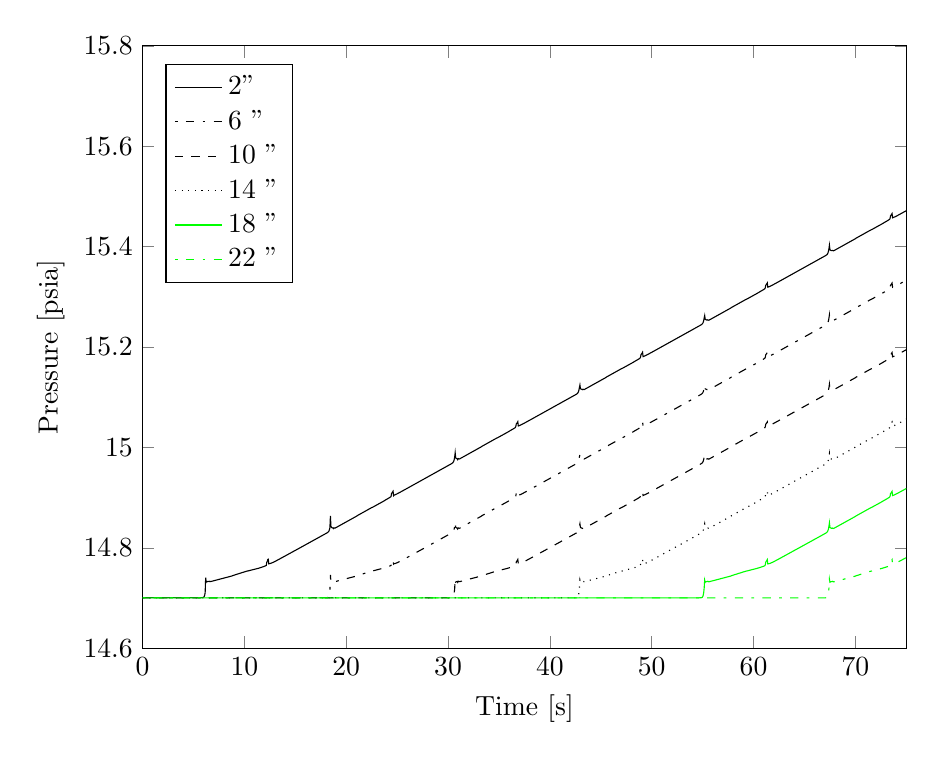
\begin{tikzpicture}

\begin{axis}[%
width=0.8\textwidth,
height=0.630967741935484\textwidth,
scale only axis,
xmin=0,
xmax=75,
xlabel={Time [s]},
ymin=14.6,
ymax=15.8,
ylabel={Pressure [psia]},
legend style={at={(0.03,0.97)},anchor=north west,draw=black,fill=white,legend cell align=left}
]
\addplot [
color=black,
solid
]
table[row sep=crcr]{
0 14.7007818222046\\
0.000862877757754177 14.7007904052734\\
0.0481183268129826 14.7007827758789\\
0.0981183275580406 14.7007827758789\\
0.148118332028389 14.7007827758789\\
0.198118329048157 14.7007827758789\\
0.248118326067925 14.7007827758789\\
0.298118323087692 14.7007827758789\\
0.348118335008621 14.7007827758789\\
0.398118317127228 14.7007827758789\\
0.448118329048157 14.7007827758789\\
0.498118340969086 14.7007827758789\\
0.548118352890015 14.7007837295532\\
0.598118305206299 14.7007837295532\\
0.648118317127228 14.7007837295532\\
0.698118329048157 14.7007837295532\\
0.748118340969086 14.7007837295532\\
0.798118352890015 14.7007837295532\\
0.848118305206299 14.7007837295532\\
0.898118317127228 14.7007837295532\\
0.948118329048157 14.7007837295532\\
0.998118340969086 14.7007837295532\\
1.04811835289001 14.7007827758789\\
1.0981183052063 14.7007827758789\\
1.14811837673187 14.7007827758789\\
1.19811832904816 14.7007827758789\\
1.24811828136444 14.7007827758789\\
1.29811835289001 14.7007827758789\\
1.3481183052063 14.7007827758789\\
1.39811837673187 14.7007827758789\\
1.44811832904816 14.7007827758789\\
1.49811828136444 14.7007827758789\\
1.54811835289001 14.7007827758789\\
1.5981183052063 14.7007827758789\\
1.64811837673187 14.7007827758789\\
1.69811832904816 14.7007827758789\\
1.74811828136444 14.7007827758789\\
1.79811835289001 14.7007827758789\\
1.8481183052063 14.7007827758789\\
1.89811837673187 14.7007827758789\\
1.94811832904816 14.7007827758789\\
1.99811828136444 14.7007827758789\\
2.04811835289001 14.7007827758789\\
2.0981183052063 14.7007827758789\\
2.14811825752258 14.7007827758789\\
2.19811820983887 14.7007827758789\\
2.24811840057373 14.7007827758789\\
2.29811835289001 14.7007827758789\\
2.3481183052063 14.7007827758789\\
2.39811825752258 14.7007827758789\\
2.44811820983887 14.7007827758789\\
2.49811840057373 14.7007827758789\\
2.54811835289001 14.7007827758789\\
2.5981183052063 14.7007827758789\\
2.64811825752258 14.7007827758789\\
2.69811820983887 14.7007827758789\\
2.74811840057373 14.7007827758789\\
2.79811835289001 14.7007827758789\\
2.8481183052063 14.7007827758789\\
2.89811825752258 14.7007827758789\\
2.94811820983887 14.7007827758789\\
2.99811840057373 14.7007827758789\\
3.04811835289001 14.7007827758789\\
3.0981183052063 14.7007827758789\\
3.14811825752258 14.7007827758789\\
3.19811820983887 14.7007827758789\\
3.24811840057373 14.7007827758789\\
3.29811835289001 14.7007827758789\\
3.3481183052063 14.7007827758789\\
3.39811825752258 14.7007827758789\\
3.44811820983887 14.7007827758789\\
3.49811840057373 14.7007827758789\\
3.54811835289001 14.7007827758789\\
3.5981183052063 14.7007827758789\\
3.64811825752258 14.7007827758789\\
3.69811820983887 14.7007827758789\\
3.74811840057373 14.7007827758789\\
3.79811835289001 14.7007827758789\\
3.8481183052063 14.7007827758789\\
3.89811825752258 14.7007827758789\\
3.94811820983887 14.7007827758789\\
3.99811840057373 14.7007827758789\\
4.04811811447144 14.7007827758789\\
4.0981183052063 14.7007827758789\\
4.14811849594116 14.7007827758789\\
4.19811820983887 14.7007827758789\\
4.24811840057373 14.7007827758789\\
4.29811811447144 14.7007827758789\\
4.3481183052063 14.7007827758789\\
4.39811849594116 14.7007827758789\\
4.44811820983887 14.7007827758789\\
4.49811840057373 14.7007827758789\\
4.54811811447144 14.7007827758789\\
4.5981183052063 14.7007827758789\\
4.64811849594116 14.7007827758789\\
4.69811820983887 14.7007827758789\\
4.74811840057373 14.7007827758789\\
4.79811811447144 14.7007827758789\\
4.8481183052063 14.7007827758789\\
4.89811849594116 14.7007827758789\\
4.94811820983887 14.7007827758789\\
4.99811840057373 14.7007827758789\\
5.04811811447144 14.7007827758789\\
5.0981183052063 14.7007827758789\\
5.14811849594116 14.7007827758789\\
5.19811820983887 14.7007827758789\\
5.24811840057373 14.7007827758789\\
5.29811811447144 14.7007827758789\\
5.3481183052063 14.7007827758789\\
5.39811849594116 14.7007827758789\\
5.44811820983887 14.7007837295532\\
5.49811840057373 14.7007837295532\\
5.54811811447144 14.7007837295532\\
5.5981183052063 14.7007846832275\\
5.64811849594116 14.7007865905762\\
5.69811820983887 14.7007904052734\\
5.74811840057373 14.700798034668\\
5.79811811447144 14.7008142471313\\
5.8481183052063 14.700852394104\\
5.89811849594116 14.7009391784668\\
5.94811820983887 14.7011461257935\\
5.99811840057373 14.7016353607178\\
6.04811811447144 14.7027750015259\\
6.0981183052063 14.7053213119507\\
6.14811849594116 14.7106494903564\\
6.19811820983887 14.7407674789429\\
6.24811840057373 14.7324676513672\\
6.29811811447144 14.7318506240845\\
6.3481183052063 14.7325630187988\\
6.39811849594116 14.732928276062\\
6.44811820983887 14.7330951690674\\
6.49811840057373 14.7331285476685\\
6.54811811447144 14.7327871322632\\
6.5981183052063 14.7332811355591\\
6.64811849594116 14.7326946258545\\
6.69811820983887 14.7328605651855\\
6.74811840057373 14.7331304550171\\
6.79811811447144 14.7333955764771\\
6.8481183052063 14.733660697937\\
6.89811849594116 14.7339267730713\\
6.94811820983887 14.7341918945313\\
6.99811840057373 14.7344570159912\\
7.04811811447144 14.7347221374512\\
7.0981183052063 14.7349872589111\\
7.14811849594116 14.7352533340454\\
7.19811820983887 14.7355184555054\\
7.24811840057373 14.7357835769653\\
7.29811811447144 14.7360486984253\\
7.3481183052063 14.7363147735596\\
7.39811849594116 14.7365798950195\\
7.44811820983887 14.7368450164795\\
7.49811840057373 14.7371110916138\\
7.54811811447144 14.7373762130737\\
7.5981183052063 14.737642288208\\
7.64811849594116 14.737907409668\\
7.69811820983887 14.7381725311279\\
7.74811840057373 14.7384386062622\\
7.79811811447144 14.7387037277222\\
7.8481183052063 14.7389698028564\\
7.89811849594116 14.7392349243164\\
7.94811820983887 14.7395009994507\\
7.99811840057373 14.7397661209106\\
8.04811859130859 14.7400321960449\\
8.09811878204346 14.7402982711792\\
8.148118019104 14.7405633926392\\
8.19811820983887 14.7408294677734\\
8.24811840057373 14.7410955429077\\
8.29811859130859 14.741361618042\\
8.34811878204346 14.741626739502\\
8.398118019104 14.7418928146362\\
8.44811820983887 14.7421588897705\\
8.49811840057373 14.7424249649048\\
8.54811859130859 14.7426910400391\\
8.59811878204346 14.7429571151733\\
8.648118019104 14.7432231903076\\
8.69811820983887 14.7434892654419\\
8.74811840057373 14.7437553405762\\
8.79811859130859 14.7441711425781\\
8.84811878204346 14.7446508407593\\
8.898118019104 14.7449808120728\\
8.94811820983887 14.745304107666\\
8.99811840057373 14.7456274032593\\
9.04811859130859 14.7459497451782\\
9.09811878204346 14.7462720870972\\
9.148118019104 14.7465944290161\\
9.19811820983887 14.7469158172607\\
9.24811840057373 14.7472372055054\\
9.29811859130859 14.7475576400757\\
9.34811878204346 14.747878074646\\
9.398118019104 14.7481985092163\\
9.44811820983887 14.7485189437866\\
9.49811840057373 14.7488384246826\\
9.54811859130859 14.7491579055786\\
9.59811878204346 14.7494773864746\\
9.648118019104 14.7497968673706\\
9.69811820983887 14.7501153945923\\
9.74811840057373 14.7504348754883\\
9.79811859130859 14.75075340271\\
9.84811878204346 14.7510719299316\\
9.898118019104 14.7513904571533\\
9.94811820983887 14.751708984375\\
9.99811840057373 14.7520275115967\\
10.0481185913086 14.7523460388184\\
10.0981187820435 14.75266456604\\
10.148118019104 14.7529821395874\\
10.1981182098389 14.7533006668091\\
10.2481184005737 14.7536096572876\\
10.2981185913086 14.7538509368896\\
10.3481187820435 14.7539186477661\\
10.398118019104 14.7541694641113\\
10.4481182098389 14.7544355392456\\
10.4981184005737 14.7547006607056\\
10.5481185913086 14.7549638748169\\
10.5981187820435 14.7552270889282\\
10.648118019104 14.7554883956909\\
10.6981182098389 14.7557487487793\\
10.7481184005737 14.7560081481934\\
10.7981185913086 14.7562665939331\\
10.8481187820435 14.7565231323242\\
10.898118019104 14.756778717041\\
10.9481182098389 14.7570323944092\\
10.9981184005737 14.757285118103\\
11.0481185913086 14.7575359344482\\
11.0981187820435 14.7577848434448\\
11.148118019104 14.7580318450928\\
11.1981182098389 14.7582759857178\\
11.2481184005737 14.7585182189941\\
11.2981185913086 14.7587585449219\\
11.3481187820435 14.759015083313\\
11.398118019104 14.7593870162964\\
11.4481182098389 14.7596683502197\\
11.4981184005737 14.7599391937256\\
11.5481185913086 14.7602977752686\\
11.5981187820435 14.7607269287109\\
11.648118019104 14.7610492706299\\
11.6981182098389 14.7613697052002\\
11.7481184005737 14.7616968154907\\
11.7981185913086 14.7620315551758\\
11.8481187820435 14.762375831604\\
11.898118019104 14.7627325057983\\
11.9481182098389 14.7631044387817\\
11.9981184005737 14.7634944915771\\
12.0481185913086 14.7639093399048\\
12.0981187820435 14.7643556594849\\
12.148118019104 14.7648525238037\\
12.1981182098389 14.7710666656494\\
12.2481184005737 14.7730360031128\\
12.2981185913086 14.7768182754517\\
12.3481187820435 14.7772245407104\\
12.398118019104 14.7679977416992\\
12.4481182098389 14.7684745788574\\
12.4981184005737 14.7686452865601\\
12.5481185913086 14.7689199447632\\
12.5981187820435 14.7692365646362\\
12.648118019104 14.7695951461792\\
12.6981182098389 14.7699918746948\\
12.7481184005737 14.7704210281372\\
12.7981185913086 14.7708768844604\\
12.8481187820435 14.7713527679443\\
12.898118019104 14.7718439102173\\
12.9481182098389 14.772346496582\\
12.9981184005737 14.7728586196899\\
13.0481185913086 14.7733774185181\\
13.0981187820435 14.7739028930664\\
13.148118019104 14.7744369506836\\
13.1981182098389 14.7749700546265\\
13.2481184005737 14.7755060195923\\
13.2981185913086 14.7760457992554\\
13.3481187820435 14.7765893936157\\
13.398118019104 14.777135848999\\
13.4481182098389 14.777684211731\\
13.4981184005737 14.7782325744629\\
13.5481185913086 14.7787847518921\\
13.5981187820435 14.7793378829956\\
13.648118019104 14.7798919677734\\
13.6981182098389 14.780445098877\\
13.7481184005737 14.7809991836548\\
13.7981185913086 14.7815542221069\\
13.8481187820435 14.7821083068848\\
13.898118019104 14.7826623916626\\
13.9481182098389 14.7832164764404\\
13.9981184005737 14.7837715148926\\
14.0481185913086 14.7843255996704\\
14.0981187820435 14.7848806381226\\
14.148118019104 14.7854347229004\\
14.1981182098389 14.7859897613525\\
14.2481184005737 14.7865447998047\\
14.2981185913086 14.7870988845825\\
14.3481187820435 14.7876539230347\\
14.398118019104 14.7882089614868\\
14.4481182098389 14.788763999939\\
14.4981184005737 14.7893190383911\\
14.5481185913086 14.7898750305176\\
14.5981187820435 14.7904300689697\\
14.648118019104 14.7909851074219\\
14.6981182098389 14.7915410995483\\
14.7481184005737 14.7920961380005\\
14.7981185913086 14.792652130127\\
14.8481187820435 14.7932081222534\\
14.898118019104 14.7937641143799\\
14.9481182098389 14.7943201065063\\
14.9981184005737 14.7948760986328\\
15.0481185913086 14.7954320907593\\
15.0981187820435 14.7959880828857\\
15.148118019104 14.7965450286865\\
15.1981182098389 14.797101020813\\
15.2481184005737 14.7976579666138\\
15.2981185913086 14.7982139587402\\
15.3481187820435 14.7987699508667\\
15.398118019104 14.7993278503418\\
15.4481182098389 14.7998867034912\\
15.4981184005737 14.8004455566406\\
15.5481185913086 14.80100440979\\
15.5981187820435 14.8015642166138\\
15.648118019104 14.8021240234375\\
15.6981182098389 14.8026828765869\\
15.7481184005737 14.8032426834106\\
15.7981185913086 14.8038024902344\\
15.8481187820435 14.8043622970581\\
15.898118019104 14.8049211502075\\
15.9481182098389 14.8054809570313\\
15.9981184005737 14.806040763855\\
16.0481185913086 14.8066005706787\\
16.0981178283691 14.8071603775024\\
16.1481189727783 14.8077201843262\\
16.1981182098389 14.8082809448242\\
16.2481174468994 14.8088407516479\\
16.2981185913086 14.8094005584717\\
16.3481178283691 14.8099603652954\\
16.3981189727783 14.8105211257935\\
16.4481182098389 14.8110809326172\\
16.4981174468994 14.8116407394409\\
16.5481185913086 14.812201499939\\
16.5981178283691 14.8127613067627\\
16.6481189727783 14.8133220672607\\
16.6981182098389 14.8138818740845\\
16.7481174468994 14.8144426345825\\
16.7981185913086 14.8150033950806\\
16.8481178283691 14.8155641555786\\
16.8981189727783 14.8161239624023\\
16.9481182098389 14.8166847229004\\
16.9981174468994 14.8172454833984\\
17.0481185913086 14.8178062438965\\
17.0981178283691 14.8183670043945\\
17.1481189727783 14.8189277648926\\
17.1981182098389 14.8194885253906\\
17.2481174468994 14.8200492858887\\
17.2981185913086 14.8206100463867\\
17.3481178283691 14.8211708068848\\
17.3981189727783 14.8217315673828\\
17.4481182098389 14.8222932815552\\
17.4981174468994 14.8228540420532\\
17.5481185913086 14.8234148025513\\
17.5981178283691 14.8239765167236\\
17.6481189727783 14.8245372772217\\
17.6981182098389 14.825098991394\\
17.7481174468994 14.8256607055664\\
17.7981185913086 14.8262214660645\\
17.8481178283691 14.8267841339111\\
17.8981189727783 14.8273468017578\\
17.9481182098389 14.8279104232788\\
17.9981174468994 14.8284778594971\\
18.0481185913086 14.8290519714355\\
18.0981178283691 14.829644203186\\
18.1481189727783 14.8302764892578\\
18.1981182098389 14.8310070037842\\
18.2481174468994 14.8319625854492\\
18.2981185913086 14.8334188461304\\
18.3481178283691 14.8358364105225\\
18.3981189727783 14.8401031494141\\
18.4481182098389 14.8634405136108\\
18.4981174468994 14.8428583145142\\
18.5481185913086 14.8407278060913\\
18.5981178283691 14.8401498794556\\
18.6481189727783 14.8397159576416\\
18.6981182098389 14.8394355773926\\
18.7481174468994 14.8382577896118\\
18.7981185913086 14.8398208618164\\
18.8481178283691 14.8393144607544\\
18.8981189727783 14.8391914367676\\
18.9481182098389 14.8397607803345\\
18.9981174468994 14.8403234481812\\
19.0481185913086 14.8408851623535\\
19.0981178283691 14.8414478302002\\
19.1481189727783 14.8420104980469\\
19.1981182098389 14.8425731658936\\
19.2481174468994 14.8431358337402\\
19.2981185913086 14.8436985015869\\
19.3481178283691 14.8442611694336\\
19.3981189727783 14.8448238372803\\
19.4481182098389 14.845386505127\\
19.4981174468994 14.8459491729736\\
19.5481185913086 14.8465118408203\\
19.5981178283691 14.847074508667\\
19.6481189727783 14.8476371765137\\
19.6981182098389 14.8481998443604\\
19.7481174468994 14.8487634658813\\
19.7981185913086 14.849326133728\\
19.8481178283691 14.8498888015747\\
19.8981189727783 14.8504524230957\\
19.9481182098389 14.8510150909424\\
19.9981174468994 14.8515787124634\\
20.0481185913086 14.8521413803101\\
20.0981178283691 14.8527050018311\\
20.1481189727783 14.8532676696777\\
20.1981182098389 14.8538312911987\\
20.2481174468994 14.8543939590454\\
20.2981185913086 14.8549575805664\\
20.3481178283691 14.8555212020874\\
20.3981189727783 14.8560838699341\\
20.4481182098389 14.8566474914551\\
20.4981174468994 14.8572111129761\\
20.5481185913086 14.8577747344971\\
20.5981178283691 14.8583383560181\\
20.6481189727783 14.8589019775391\\
20.6981182098389 14.8594655990601\\
20.7481174468994 14.8600282669067\\
20.7981185913086 14.8605918884277\\
20.8481178283691 14.8611555099487\\
20.8981189727783 14.861720085144\\
20.9481182098389 14.862283706665\\
20.9981174468994 14.862847328186\\
21.0481185913086 14.8635883331299\\
21.0981178283691 14.864278793335\\
21.1481189727783 14.8648443222046\\
21.1981182098389 14.8654079437256\\
21.2481174468994 14.8659715652466\\
21.2981185913086 14.8665361404419\\
21.3481178283691 14.8670997619629\\
21.3981189727783 14.8676643371582\\
21.4481182098389 14.8682289123535\\
21.4981174468994 14.8687934875488\\
21.5481185913086 14.8693580627441\\
21.5981178283691 14.8699226379395\\
21.6481189727783 14.8704872131348\\
21.6981182098389 14.8710517883301\\
21.7481174468994 14.8716173171997\\
21.7981185913086 14.872181892395\\
21.8481178283691 14.8727474212646\\
21.8981189727783 14.87331199646\\
21.9481182098389 14.8738775253296\\
21.9981174468994 14.8744430541992\\
22.0481185913086 14.8750085830688\\
22.0981178283691 14.8755750656128\\
22.1481189727783 14.8761405944824\\
22.1981182098389 14.8767070770264\\
22.2481174468994 14.877272605896\\
22.2981185913086 14.8778390884399\\
22.3481178283691 14.8784055709839\\
22.3981189727783 14.8789720535278\\
22.4481182098389 14.8795394897461\\
22.4981174468994 14.8800992965698\\
22.5481185913086 14.8806104660034\\
22.5981178283691 14.8809404373169\\
22.6481189727783 14.8814888000488\\
22.6981182098389 14.8820505142212\\
22.7481174468994 14.8826103210449\\
22.7981185913086 14.8831701278687\\
22.8481178283691 14.8837299346924\\
22.8981189727783 14.8842887878418\\
22.9481182098389 14.8848485946655\\
22.9981174468994 14.8854074478149\\
23.0481185913086 14.8859663009644\\
23.0981178283691 14.8865251541138\\
23.1481189727783 14.8870830535889\\
23.1981182098389 14.887640953064\\
23.2481174468994 14.8881988525391\\
23.2981185913086 14.8887557983398\\
23.3481178283691 14.8893136978149\\
23.3981189727783 14.8898696899414\\
23.4481182098389 14.8904256820679\\
23.4981174468994 14.8909816741943\\
23.5481185913086 14.8915367126465\\
23.5981178283691 14.8921089172363\\
23.6481189727783 14.8927640914917\\
23.6981182098389 14.8933391571045\\
23.7481174468994 14.8939056396484\\
23.7981185913086 14.8945360183716\\
23.8481178283691 14.8952054977417\\
23.8981189727783 14.8957862854004\\
23.9481182098389 14.8963661193848\\
23.9981174468994 14.8969507217407\\
24.0481185913086 14.8975391387939\\
24.0981178283691 14.8981342315674\\
24.1481189727783 14.8987369537354\\
24.1981182098389 14.8993482589722\\
24.2481174468994 14.8999719619751\\
24.2981185913086 14.9006118774414\\
24.3481178283691 14.9012727737427\\
24.3981189727783 14.9019622802734\\
24.4481182098389 14.9080991744995\\
24.4981174468994 14.9095907211304\\
24.5481185913086 14.9110221862793\\
24.5981178283691 14.9127492904663\\
24.6481189727783 14.9038639068604\\
24.6981182098389 14.9049654006958\\
24.7481174468994 14.9053144454956\\
24.7981185913086 14.9057321548462\\
24.8481178283691 14.9061670303345\\
24.8981189727783 14.906623840332\\
24.9481182098389 14.9071035385132\\
24.9981174468994 14.907603263855\\
25.0481185913086 14.9081182479858\\
25.0981178283691 14.9086456298828\\
25.1481189727783 14.9091806411743\\
25.1981182098389 14.909722328186\\
25.2481174468994 14.910267829895\\
25.2981185913086 14.9108171463013\\
25.3481178283691 14.9113683700562\\
25.3981189727783 14.911922454834\\
25.4481182098389 14.9124774932861\\
25.4981174468994 14.9130363464355\\
25.5481185913086 14.9135913848877\\
25.5981178283691 14.9141473770142\\
25.6481189727783 14.9147043228149\\
25.6981182098389 14.9152631759644\\
25.7481174468994 14.9158220291138\\
25.7981185913086 14.9163827896118\\
25.8481178283691 14.9169435501099\\
25.8981189727783 14.9175033569336\\
25.9481182098389 14.9180660247803\\
25.9981174468994 14.9186296463013\\
26.0481185913086 14.9191932678223\\
26.0981178283691 14.9197568893433\\
26.1481189727783 14.9203214645386\\
26.1981182098389 14.9208850860596\\
26.2481174468994 14.9214487075806\\
26.2981185913086 14.9220132827759\\
26.3481178283691 14.9225769042969\\
26.3981189727783 14.9231405258179\\
26.4481182098389 14.9237051010132\\
26.4981174468994 14.9242687225342\\
26.5481185913086 14.9248323440552\\
26.5981178283691 14.9253969192505\\
26.6481189727783 14.9259605407715\\
26.6981182098389 14.9265251159668\\
26.7481174468994 14.9270887374878\\
26.7981185913086 14.9276523590088\\
26.8481178283691 14.9282169342041\\
26.8981189727783 14.9287805557251\\
26.9481182098389 14.9293441772461\\
26.9981174468994 14.9299087524414\\
27.0481185913086 14.9304723739624\\
27.0981178283691 14.9310359954834\\
27.1481189727783 14.9316005706787\\
27.1981182098389 14.9321641921997\\
27.2481174468994 14.9327278137207\\
27.2981185913086 14.9332914352417\\
27.3481178283691 14.933856010437\\
27.3981189727783 14.934419631958\\
27.4481182098389 14.934983253479\\
27.4981174468994 14.9355478286743\\
27.5481185913086 14.9361114501953\\
27.5981178283691 14.9366750717163\\
27.6481189727783 14.9372396469116\\
27.6981182098389 14.9378032684326\\
27.7481174468994 14.9383668899536\\
27.7981185913086 14.9389314651489\\
27.8481178283691 14.9394950866699\\
27.8981189727783 14.9400587081909\\
27.9481182098389 14.9406223297119\\
27.9981174468994 14.9411869049072\\
28.0481185913086 14.9417505264282\\
28.0981178283691 14.9423141479492\\
28.1481189727783 14.9428787231445\\
28.1981182098389 14.9434366226196\\
28.2481174468994 14.9439992904663\\
28.2981185913086 14.9445629119873\\
28.3481178283691 14.9451265335083\\
28.3981189727783 14.9456901550293\\
28.4481182098389 14.9462547302246\\
28.4981174468994 14.9468183517456\\
28.5481185913086 14.9473819732666\\
28.5981178283691 14.9479465484619\\
28.6481189727783 14.9485101699829\\
28.6981182098389 14.9490737915039\\
28.7481174468994 14.9496383666992\\
28.7981185913086 14.9502019882202\\
28.8481178283691 14.9507665634155\\
28.8981189727783 14.9513301849365\\
28.9481182098389 14.9518938064575\\
28.9981174468994 14.9524583816528\\
29.0481185913086 14.9530220031738\\
29.0981178283691 14.9535865783691\\
29.1481189727783 14.9541501998901\\
29.1981182098389 14.9547138214111\\
29.2481174468994 14.9552783966064\\
29.2981185913086 14.9558420181274\\
29.3481178283691 14.9564065933228\\
29.3981189727783 14.9569702148438\\
29.4481182098389 14.9575347900391\\
29.4981174468994 14.9580984115601\\
29.5481185913086 14.9586620330811\\
29.5981178283691 14.9592266082764\\
29.6481189727783 14.9597902297974\\
29.6981182098389 14.9603548049927\\
29.7481174468994 14.9609184265137\\
29.7981185913086 14.9614820480347\\
29.8481178283691 14.96204662323\\
29.8981189727783 14.962610244751\\
29.9481182098389 14.9631748199463\\
29.9981174468994 14.9637393951416\\
30.0481185913086 14.9643039703369\\
30.0981178283691 14.9648685455322\\
30.1481189727783 14.9654340744019\\
30.1981182098389 14.9660015106201\\
30.2481174468994 14.96657371521\\
30.2981185913086 14.9671564102173\\
30.3481178283691 14.9677648544312\\
30.3981189727783 14.9684324264526\\
30.4481182098389 14.9692440032959\\
30.4981174468994 14.9703798294067\\
30.5481185913086 14.9722156524658\\
30.5981178283691 14.9753637313843\\
30.6481189727783 14.9805841445923\\
30.6981182098389 14.9893856048584\\
30.7481174468994 14.9792137145996\\
30.7981185913086 14.9783201217651\\
30.8481178283691 14.9778032302856\\
30.8981189727783 14.977442741394\\
30.9481182098389 14.9756002426147\\
30.9981174468994 14.9778280258179\\
31.0481185913086 14.9774351119995\\
31.0981178283691 14.9769945144653\\
31.1481189727783 14.9773244857788\\
31.1981182098389 14.9778985977173\\
31.2481174468994 14.9784622192383\\
31.2981185913086 14.9790258407593\\
31.3481178283691 14.9795904159546\\
31.3981189727783 14.9801540374756\\
31.4481182098389 14.9807186126709\\
31.4981174468994 14.9812822341919\\
31.5481185913086 14.9818468093872\\
31.5981178283691 14.9824113845825\\
31.6481189727783 14.9829750061035\\
31.6981182098389 14.9835395812988\\
31.7481174468994 14.9841041564941\\
31.7981185913086 14.9846677780151\\
31.8481178283691 14.9852323532104\\
31.8981189727783 14.9857969284058\\
31.9481182098389 14.9863605499268\\
31.9981174468994 14.9869251251221\\
32.0481185913086 14.9874897003174\\
32.0981178283691 14.9880542755127\\
32.1481170654297 14.9886178970337\\
32.1981201171875 14.989182472229\\
32.248119354248 14.9897470474243\\
32.2981185913086 14.9903116226196\\
32.3481178283691 14.9908752441406\\
32.3981170654297 14.9914398193359\\
32.4481201171875 14.9920043945313\\
32.498119354248 14.9925689697266\\
32.5481185913086 14.9931335449219\\
32.5981178283691 14.9936981201172\\
32.6481170654297 14.9942626953125\\
32.6981201171875 14.9948272705078\\
32.748119354248 14.9953918457031\\
32.7981185913086 14.9959564208984\\
32.8481178283691 14.9965200424194\\
32.8981170654297 14.9970846176147\\
32.9481201171875 14.9976491928101\\
32.998119354248 14.9982147216797\\
33.0481185913086 14.998779296875\\
33.0981178283691 14.9993438720703\\
33.1481170654297 14.9999084472656\\
33.1981201171875 15.0004730224609\\
33.248119354248 15.0010375976563\\
33.2981185913086 15.0018739700317\\
33.3481178283691 15.0024690628052\\
33.3981170654297 15.0030326843262\\
33.4481201171875 15.0035972595215\\
33.498119354248 15.0041627883911\\
33.5481185913086 15.0047273635864\\
33.5981178283691 15.0052928924561\\
33.6481170654297 15.0058574676514\\
33.6981201171875 15.006422996521\\
33.748119354248 15.0069885253906\\
33.7981185913086 15.0075531005859\\
33.8481178283691 15.0081186294556\\
33.8981170654297 15.0086841583252\\
33.9481201171875 15.0092496871948\\
33.998119354248 15.0098161697388\\
34.0481185913086 15.0103816986084\\
34.0981178283691 15.010947227478\\
34.1481170654297 15.011513710022\\
34.1981201171875 15.0120792388916\\
34.248119354248 15.0126457214355\\
34.2981185913086 15.0132112503052\\
34.3481178283691 15.0137777328491\\
34.3981170654297 15.0143442153931\\
34.4481201171875 15.0149116516113\\
34.498119354248 15.0154781341553\\
34.5481185913086 15.0160446166992\\
34.5981178283691 15.0166120529175\\
34.6481170654297 15.0171794891357\\
34.6981201171875 15.017746925354\\
34.748119354248 15.0182847976685\\
34.7981185913086 15.0187902450562\\
34.8481178283691 15.0191373825073\\
34.8981170654297 15.0197019577026\\
34.9481201171875 15.0202627182007\\
34.998119354248 15.0208234786987\\
35.0481185913086 15.0213832855225\\
35.0981178283691 15.0219440460205\\
35.1481170654297 15.0225038528442\\
35.1981201171875 15.023063659668\\
35.248119354248 15.0236234664917\\
35.2981185913086 15.0241832733154\\
35.3481178283691 15.0247421264648\\
35.3981170654297 15.0253009796143\\
35.4481201171875 15.0258598327637\\
35.498119354248 15.0264186859131\\
35.5481185913086 15.0269765853882\\
35.5981178283691 15.0275344848633\\
35.6481170654297 15.0280923843384\\
35.6981201171875 15.0286493301392\\
35.748119354248 15.0292062759399\\
35.7981185913086 15.0297622680664\\
35.8481178283691 15.030369758606\\
35.8981170654297 15.030987739563\\
35.9481201171875 15.0315570831299\\
35.998119354248 15.0321245193481\\
36.0481185913086 15.0327949523926\\
36.0981178283691 15.0334129333496\\
36.1481170654297 15.0339908599854\\
36.1981201171875 15.0345726013184\\
36.248119354248 15.0351572036743\\
36.2981185913086 15.0357475280762\\
36.3481178283691 15.0363435745239\\
36.3981170654297 15.0369482040405\\
36.4481201171875 15.037561416626\\
36.498119354248 15.0381889343262\\
36.5481185913086 15.0388317108154\\
36.5981178283691 15.0394983291626\\
36.6481170654297 15.0413684844971\\
36.6981201171875 15.0466718673706\\
36.748119354248 15.0479555130005\\
36.7981185913086 15.0494518280029\\
36.8481178283691 15.0512561798096\\
36.8981170654297 15.042685508728\\
36.9481201171875 15.0431299209595\\
36.998119354248 15.0434913635254\\
37.0481185913086 15.0439138412476\\
37.0981178283691 15.0443544387817\\
37.1481170654297 15.0448169708252\\
37.1981201171875 15.0453023910522\\
37.248119354248 15.0458068847656\\
37.2981185913086 15.0463256835938\\
37.3481178283691 15.0468549728394\\
37.3981170654297 15.0473928451538\\
37.4481201171875 15.0479354858398\\
37.498119354248 15.0484819412231\\
37.5481185913086 15.0490322113037\\
37.5981178283691 15.0495843887329\\
37.6481170654297 15.0501384735107\\
37.6981201171875 15.0506935119629\\
37.748119354248 15.0512533187866\\
37.7981185913086 15.0518093109131\\
37.8481178283691 15.0523653030396\\
37.8981170654297 15.0529222488403\\
37.9481201171875 15.0534811019897\\
37.998119354248 15.0540409088135\\
38.0481185913086 15.0546016693115\\
38.0981178283691 15.0551624298096\\
38.1481170654297 15.0557241439819\\
38.1981201171875 15.05628490448\\
38.248119354248 15.056848526001\\
38.2981185913086 15.057412147522\\
38.3481178283691 15.0579767227173\\
38.3981170654297 15.0585403442383\\
38.4481201171875 15.0591049194336\\
38.498119354248 15.0596685409546\\
38.5481185913086 15.0602321624756\\
38.5981178283691 15.0607967376709\\
38.6481170654297 15.0613613128662\\
38.6981201171875 15.0619249343872\\
38.748119354248 15.0624895095825\\
38.7981185913086 15.0630531311035\\
38.8481178283691 15.0636177062988\\
38.8981170654297 15.0641813278198\\
38.9481201171875 15.0647459030151\\
38.998119354248 15.0653095245361\\
39.0481185913086 15.0658740997314\\
39.0981178283691 15.0664377212524\\
39.1481170654297 15.0670022964478\\
39.1981201171875 15.0675659179688\\
39.248119354248 15.0681304931641\\
39.2981185913086 15.0686941146851\\
39.3481178283691 15.0692586898804\\
39.3981170654297 15.0698223114014\\
39.4481201171875 15.0703868865967\\
39.498119354248 15.0709505081177\\
39.5481185913086 15.0715141296387\\
39.5981178283691 15.072078704834\\
39.6481170654297 15.072642326355\\
39.6981201171875 15.0732069015503\\
39.748119354248 15.0737705230713\\
39.7981185913086 15.0743350982666\\
39.8481178283691 15.0748987197876\\
39.8981170654297 15.0754632949829\\
39.9481201171875 15.0760269165039\\
39.998119354248 15.0765914916992\\
40.0481185913086 15.0771551132202\\
40.0981178283691 15.0777187347412\\
40.1481170654297 15.0782833099365\\
40.1981201171875 15.0788469314575\\
40.248119354248 15.0794115066528\\
40.2981185913086 15.0799751281738\\
40.3481178283691 15.0805397033691\\
40.3981170654297 15.0811033248901\\
40.4481201171875 15.0816679000854\\
40.498119354248 15.0822315216064\\
40.5481185913086 15.0827951431274\\
40.5981178283691 15.0833597183228\\
40.6481170654297 15.0839233398438\\
40.6981201171875 15.0845289230347\\
40.748119354248 15.0850477218628\\
40.7981185913086 15.0856103897095\\
40.8481178283691 15.0861730575562\\
40.8981170654297 15.0867366790771\\
40.9481201171875 15.0873003005981\\
40.998119354248 15.0878648757935\\
41.0481185913086 15.0884284973145\\
41.0981178283691 15.0889930725098\\
41.1481170654297 15.0895566940308\\
41.1981201171875 15.0901212692261\\
41.248119354248 15.0906848907471\\
41.2981185913086 15.0912494659424\\
41.3481178283691 15.0918130874634\\
41.3981170654297 15.0923776626587\\
41.4481201171875 15.0929412841797\\
41.498119354248 15.093505859375\\
41.5481185913086 15.094069480896\\
41.5981178283691 15.0946340560913\\
41.6481170654297 15.0951976776123\\
41.6981201171875 15.0957622528076\\
41.748119354248 15.0963268280029\\
41.7981185913086 15.0968904495239\\
41.8481178283691 15.0974550247192\\
41.8981170654297 15.0980186462402\\
41.9481201171875 15.0985832214355\\
41.998119354248 15.0991468429565\\
42.0481185913086 15.0997114181519\\
42.0981178283691 15.1002750396729\\
42.1481170654297 15.1008396148682\\
42.1981201171875 15.1014041900635\\
42.248119354248 15.1019678115845\\
42.2981185913086 15.1025323867798\\
42.3481178283691 15.1030979156494\\
42.3981170654297 15.103663444519\\
42.4481201171875 15.1042318344116\\
42.498119354248 15.1048049926758\\
42.5481185913086 15.1053905487061\\
42.5981178283691 15.1060037612915\\
42.6481170654297 15.1066846847534\\
42.6981201171875 15.1075248718262\\
42.748119354248 15.1087265014648\\
42.7981185913086 15.1106958389282\\
42.8481178283691 15.1140747070313\\
42.8981170654297 15.1195755004883\\
42.9481201171875 15.1244058609009\\
42.998119354248 15.1171503067017\\
43.0481185913086 15.1164035797119\\
43.0981178283691 15.1159048080444\\
43.1481170654297 15.1155652999878\\
43.1981201171875 15.1149959564209\\
43.248119354248 15.1159811019897\\
43.2981185913086 15.1155271530151\\
43.3481178283691 15.1151285171509\\
43.3981170654297 15.1155605316162\\
43.4481201171875 15.1161308288574\\
43.498119354248 15.1166944503784\\
43.5481185913086 15.1172590255737\\
43.5981178283691 15.1178226470947\\
43.6481170654297 15.11838722229\\
43.6981201171875 15.118950843811\\
43.748119354248 15.1195154190063\\
43.7981185913086 15.1200799942017\\
43.8481178283691 15.120644569397\\
43.8981170654297 15.121208190918\\
43.9481201171875 15.1217727661133\\
43.998119354248 15.1223373413086\\
44.0481185913086 15.1229019165039\\
44.0981178283691 15.1234655380249\\
44.1481170654297 15.1240301132202\\
44.1981201171875 15.1245946884155\\
44.248119354248 15.1251592636108\\
44.2981185913086 15.1257238388062\\
44.3481178283691 15.1262884140015\\
44.3981170654297 15.1268520355225\\
44.4481201171875 15.1274166107178\\
44.498119354248 15.1279811859131\\
44.5481185913086 15.1285457611084\\
44.5981178283691 15.1291103363037\\
44.6481170654297 15.129674911499\\
44.6981201171875 15.1302394866943\\
44.748119354248 15.1308040618896\\
44.7981185913086 15.131368637085\\
44.8481178283691 15.1319332122803\\
44.8981170654297 15.1324977874756\\
44.9481201171875 15.1330623626709\\
44.998119354248 15.1336269378662\\
45.0481185913086 15.1341915130615\\
45.0981178283691 15.1347560882568\\
45.1481170654297 15.1353206634521\\
45.1981201171875 15.1358852386475\\
45.248119354248 15.1364498138428\\
45.2981185913086 15.1370143890381\\
45.3481178283691 15.1375799179077\\
45.3981170654297 15.138144493103\\
45.4481201171875 15.1387090682983\\
45.498119354248 15.139274597168\\
45.5481185913086 15.1401195526123\\
45.5981178283691 15.1407032012939\\
45.6481170654297 15.1412677764893\\
45.6981201171875 15.1418323516846\\
45.748119354248 15.1423978805542\\
45.7981185913086 15.1429624557495\\
45.8481178283691 15.1435279846191\\
45.8981170654297 15.1440935134888\\
45.9481201171875 15.1446580886841\\
45.998119354248 15.1452236175537\\
46.0481185913086 15.1457891464233\\
46.0981178283691 15.146354675293\\
46.1481170654297 15.1469202041626\\
46.1981201171875 15.1474857330322\\
46.248119354248 15.1480522155762\\
46.2981185913086 15.1486177444458\\
46.3481178283691 15.1491842269897\\
46.3981170654297 15.1497497558594\\
46.4481201171875 15.1503162384033\\
46.498119354248 15.1508827209473\\
46.5481185913086 15.1514482498169\\
46.5981178283691 15.1520147323608\\
46.6481170654297 15.1525821685791\\
46.6981201171875 15.153148651123\\
46.748119354248 15.153715133667\\
46.7981185913086 15.1542825698853\\
46.8481178283691 15.1548500061035\\
46.8981170654297 15.1554164886475\\
46.9481201171875 15.15598487854\\
46.998119354248 15.1565198898315\\
47.0481185913086 15.1569967269897\\
47.0981178283691 15.157377243042\\
47.1481170654297 15.1579418182373\\
47.1981201171875 15.1585035324097\\
47.248119354248 15.1590642929077\\
47.2981185913086 15.1596250534058\\
47.3481178283691 15.1601848602295\\
47.3981170654297 15.1607456207275\\
47.4481201171875 15.1613054275513\\
47.498119354248 15.1618661880493\\
47.5481185913086 15.162425994873\\
47.5981178283691 15.1629848480225\\
47.6481170654297 15.1635446548462\\
47.6981201171875 15.1641035079956\\
47.748119354248 15.164662361145\\
47.7981185913086 15.1652212142944\\
47.8481178283691 15.1657800674438\\
47.8981170654297 15.1663379669189\\
47.9481201171875 15.166895866394\\
47.998119354248 15.1674528121948\\
48.0481185913086 15.1680097579956\\
48.0981178283691 15.1686220169067\\
48.1481170654297 15.1692304611206\\
48.1981201171875 15.1697988510132\\
48.248119354248 15.1703672409058\\
48.2981185913086 15.1710376739502\\
48.3481178283691 15.1716461181641\\
48.3981170654297 15.1722240447998\\
48.4481201171875 15.1728057861328\\
48.498119354248 15.1733903884888\\
48.5481185913086 15.1739807128906\\
48.5981178283691 15.1745777130127\\
48.6481170654297 15.175181388855\\
48.6981201171875 15.1757965087891\\
48.748119354248 15.1764230728149\\
48.7981185913086 15.1770677566528\\
48.8481178283691 15.1777353286743\\
48.8981170654297 15.1800975799561\\
48.9481201171875 15.1849613189697\\
48.998119354248 15.1862268447876\\
49.0481185913086 15.1877384185791\\
49.0981178283691 15.1895618438721\\
49.1481170654297 15.1808500289917\\
49.1981201171875 15.1813564300537\\
49.248119354248 15.1817207336426\\
49.2981185913086 15.1821441650391\\
49.3481178283691 15.1825866699219\\
49.3981170654297 15.183051109314\\
49.4481201171875 15.1835384368896\\
49.498119354248 15.1840438842773\\
49.5481185913086 15.1845626831055\\
49.5981178283691 15.1850929260254\\
49.6481170654297 15.1856307983398\\
49.6981201171875 15.1861743927002\\
49.748119354248 15.1867218017578\\
49.7981185913086 15.1872711181641\\
49.8481178283691 15.1878242492676\\
49.8981170654297 15.1883783340454\\
49.9481201171875 15.1889333724976\\
49.998119354248 15.1894941329956\\
50.0481185913086 15.1900491714478\\
50.0981178283691 15.1906051635742\\
50.1481170654297 15.1911630630493\\
50.1981201171875 15.1917219161987\\
50.248119354248 15.1922817230225\\
50.2981185913086 15.1928424835205\\
50.3481178283691 15.1934032440186\\
50.3981170654297 15.1939649581909\\
50.4481201171875 15.194525718689\\
50.498119354248 15.19508934021\\
50.5481185913086 15.195652961731\\
50.5981178283691 15.196216583252\\
50.6481170654297 15.1967811584473\\
50.6981201171875 15.1973447799683\\
50.748119354248 15.1979093551636\\
50.7981185913086 15.1984729766846\\
50.8481178283691 15.1990375518799\\
50.8981170654297 15.1996011734009\\
50.9481201171875 15.2001657485962\\
50.998119354248 15.2007303237915\\
51.0481185913086 15.2012939453125\\
51.0981178283691 15.2018585205078\\
51.1481170654297 15.2024221420288\\
51.1981201171875 15.2029867172241\\
51.248119354248 15.2035503387451\\
51.2981185913086 15.2041149139404\\
51.3481178283691 15.2046794891357\\
51.3981170654297 15.2052431106567\\
51.4481201171875 15.2058076858521\\
51.498119354248 15.206371307373\\
51.5481185913086 15.2069358825684\\
51.5981178283691 15.2074995040894\\
51.6481170654297 15.2080640792847\\
51.6981201171875 15.2086277008057\\
51.748119354248 15.209192276001\\
51.7981185913086 15.209755897522\\
51.8481178283691 15.2103204727173\\
51.8981170654297 15.2108840942383\\
51.9481201171875 15.2114486694336\\
51.998119354248 15.2120122909546\\
52.0481185913086 15.2125768661499\\
52.0981178283691 15.2131404876709\\
52.1481170654297 15.2137050628662\\
52.1981201171875 15.2142686843872\\
52.248119354248 15.2148332595825\\
52.2981185913086 15.2153978347778\\
52.3481178283691 15.2159614562988\\
52.3981170654297 15.2165260314941\\
52.4481201171875 15.2170896530151\\
52.498119354248 15.2176542282104\\
52.5481185913086 15.2182178497314\\
52.5981178283691 15.2187824249268\\
52.6481170654297 15.2193460464478\\
52.6981201171875 15.2199096679688\\
52.748119354248 15.2204742431641\\
52.7981185913086 15.2210378646851\\
52.8481178283691 15.2216024398804\\
52.8981170654297 15.2221660614014\\
52.9481201171875 15.2227306365967\\
52.998119354248 15.2232942581177\\
53.0481185913086 15.223858833313\\
53.0981178283691 15.224422454834\\
53.1481170654297 15.2249870300293\\
53.1981201171875 15.225549697876\\
53.248119354248 15.2261095046997\\
53.2981185913086 15.2266731262207\\
53.3481178283691 15.2272367477417\\
53.3981170654297 15.2278003692627\\
53.4481201171875 15.2283639907837\\
53.498119354248 15.228928565979\\
53.5481185913086 15.2294921875\\
53.5981178283691 15.2300567626953\\
53.6481170654297 15.2306203842163\\
53.6981201171875 15.2311849594116\\
53.748119354248 15.2317495346069\\
53.7981185913086 15.2323131561279\\
53.8481178283691 15.2328777313232\\
53.8981170654297 15.2334413528442\\
53.9481201171875 15.2340059280396\\
53.998119354248 15.2345695495605\\
54.0481185913086 15.2351341247559\\
54.0981178283691 15.2356986999512\\
54.1481170654297 15.2362623214722\\
54.1981201171875 15.2368268966675\\
54.248119354248 15.2373905181885\\
54.2981185913086 15.2379550933838\\
54.3481178283691 15.2385187149048\\
54.3981170654297 15.2390832901001\\
54.4481201171875 15.2396478652954\\
54.498119354248 15.2402124404907\\
54.5481185913086 15.240777015686\\
54.5981178283691 15.2413415908813\\
54.6481170654297 15.2419080734253\\
54.6981201171875 15.2424764633179\\
54.748119354248 15.243049621582\\
54.7981185913086 15.2436351776123\\
54.8481178283691 15.2442493438721\\
54.8981170654297 15.2449312210083\\
54.9481201171875 15.2457752227783\\
54.998119354248 15.2469835281372\\
55.0481185913086 15.248966217041\\
55.0981178283691 15.252368927002\\
55.1481170654297 15.2578964233398\\
55.1981201171875 15.2625751495361\\
55.248119354248 15.2553720474243\\
55.2981185913086 15.2546329498291\\
55.3481178283691 15.2541370391846\\
55.3981170654297 15.2537994384766\\
55.4481201171875 15.2537183761597\\
55.498119354248 15.2541942596436\\
55.5481185913086 15.253758430481\\
55.5981178283691 15.2533655166626\\
55.6481170654297 15.2538061141968\\
55.6981201171875 15.254376411438\\
55.748119354248 15.254940032959\\
55.7981185913086 15.2555046081543\\
55.8481178283691 15.2560682296753\\
55.8981170654297 15.2566328048706\\
55.9481201171875 15.2571973800659\\
55.998119354248 15.2577610015869\\
56.0481185913086 15.2583255767822\\
56.0981178283691 15.2588901519775\\
56.1481170654297 15.2594537734985\\
56.1981201171875 15.2600183486938\\
56.248119354248 15.2605829238892\\
56.2981185913086 15.2611474990845\\
56.3481178283691 15.2617120742798\\
56.3981170654297 15.2622766494751\\
56.4481201171875 15.2628402709961\\
56.498119354248 15.2634048461914\\
56.5481185913086 15.2639694213867\\
56.5981178283691 15.264533996582\\
56.6481170654297 15.2650985717773\\
56.6981201171875 15.2656631469727\\
56.748119354248 15.266227722168\\
56.7981185913086 15.266791343689\\
56.8481178283691 15.2673559188843\\
56.8981170654297 15.2679204940796\\
56.9481201171875 15.2684850692749\\
56.998119354248 15.2690496444702\\
57.0481185913086 15.2696142196655\\
57.0981178283691 15.2701787948608\\
57.1481170654297 15.2707443237305\\
57.1981201171875 15.2713088989258\\
57.248119354248 15.2718734741211\\
57.2981185913086 15.2724380493164\\
57.3481178283691 15.2730026245117\\
57.3981170654297 15.273567199707\\
57.4481201171875 15.2741317749023\\
57.498119354248 15.2746963500977\\
57.5481185913086 15.2752618789673\\
57.5981178283691 15.2758264541626\\
57.6481170654297 15.2763910293579\\
57.6981201171875 15.2769556045532\\
57.748119354248 15.2775211334229\\
57.7981185913086 15.2783651351929\\
57.8481178283691 15.2789487838745\\
57.8981170654297 15.2795133590698\\
57.9481201171875 15.2800788879395\\
57.998119354248 15.2806434631348\\
58.0481185913086 15.2812089920044\\
58.0981178283691 15.2817735671997\\
58.1481170654297 15.2823390960693\\
58.1981201171875 15.282904624939\\
58.248119354248 15.2834701538086\\
58.2981185913086 15.2840356826782\\
58.3481178283691 15.2846012115479\\
58.3981170654297 15.2851667404175\\
58.4481201171875 15.2857322692871\\
58.498119354248 15.2862987518311\\
58.5481185913086 15.2868642807007\\
58.5981178283691 15.2874307632446\\
58.6481170654297 15.2879962921143\\
58.6981201171875 15.2885627746582\\
58.748119354248 15.2891292572021\\
58.7981185913086 15.2896957397461\\
58.8481178283691 15.29026222229\\
58.8981170654297 15.290828704834\\
58.9481201171875 15.2913951873779\\
58.998119354248 15.2919626235962\\
59.0481185913086 15.2925291061401\\
59.0981178283691 15.2930965423584\\
59.1481170654297 15.2936639785767\\
59.1981201171875 15.2942314147949\\
59.248119354248 15.2947702407837\\
59.2981185913086 15.2952489852905\\
59.3481178283691 15.2956256866455\\
59.3981170654297 15.2961912155151\\
59.4481201171875 15.2967529296875\\
59.498119354248 15.2973136901855\\
59.5481185913086 15.2978744506836\\
59.5981178283691 15.2984352111816\\
59.6481170654297 15.2989959716797\\
59.6981201171875 15.2995557785034\\
59.748119354248 15.3001165390015\\
59.7981185913086 15.3006763458252\\
59.8481178283691 15.3012361526489\\
59.8981170654297 15.3017959594727\\
59.9481201171875 15.3023548126221\\
59.998119354248 15.3029136657715\\
60.0467147827148 15.3034572601318\\
60.0967140197754 15.3040161132813\\
60.1467132568359 15.3045740127563\\
60.1967124938965 15.3051328659058\\
60.246711730957 15.3056907653809\\
60.2967147827148 15.3062477111816\\
60.3467140197754 15.3068542480469\\
60.3967132568359 15.3074636459351\\
60.4467124938965 15.3080320358276\\
60.496711730957 15.3086004257202\\
60.5467147827148 15.3092622756958\\
60.5967140197754 15.3098726272583\\
60.6467132568359 15.310450553894\\
60.6967124938965 15.3110313415527\\
60.746711730957 15.311616897583\\
60.7967147827148 15.3122062683105\\
60.8467140197754 15.3128023147583\\
60.8967132568359 15.3134059906006\\
60.9467124938965 15.3140201568604\\
60.996711730957 15.3146467208862\\
61.0467147827148 15.3152894973755\\
61.0967140197754 15.3159551620483\\
61.1467132568359 15.3179540634155\\
61.1967124938965 15.3231449127197\\
61.246711730957 15.3244161605835\\
61.2967147827148 15.3259134292603\\
61.3467140197754 15.3277187347412\\
61.3967132568359 15.3191289901733\\
61.4467124938965 15.3195953369141\\
61.496711730957 15.3199577331543\\
61.5467147827148 15.3203811645508\\
61.5967140197754 15.320821762085\\
61.6467132568359 15.3212862014771\\
61.6967124938965 15.3217725753784\\
61.746711730957 15.3222770690918\\
61.7967147827148 15.3227968215942\\
61.8467140197754 15.3233261108398\\
61.8967132568359 15.3238639831543\\
61.9467124938965 15.3244066238403\\
61.996711730957 15.3249540328979\\
62.0467147827148 15.3255043029785\\
62.0967140197754 15.3260564804077\\
62.1467132568359 15.3266105651855\\
62.1967124938965 15.327166557312\\
62.246711730957 15.3277263641357\\
62.2967147827148 15.3282814025879\\
62.3467140197754 15.3288383483887\\
62.3967132568359 15.3293952941895\\
62.4467124938965 15.3299541473389\\
62.496711730957 15.3305139541626\\
62.5467147827148 15.3310747146606\\
62.5967140197754 15.3316354751587\\
62.6467132568359 15.3321971893311\\
62.6967124938965 15.3327589035034\\
62.746711730957 15.3333206176758\\
62.7967147827148 15.3338842391968\\
62.8467140197754 15.3344488143921\\
62.8967132568359 15.3350124359131\\
62.9467124938965 15.3355770111084\\
62.996711730957 15.3361406326294\\
63.0467147827148 15.3367052078247\\
63.0967140197754 15.3372688293457\\
63.1467132568359 15.337833404541\\
63.1967124938965 15.3383979797363\\
63.246711730957 15.3389616012573\\
63.2967147827148 15.3395261764526\\
63.3467140197754 15.3400907516479\\
63.3967132568359 15.3406543731689\\
63.4467124938965 15.3412189483643\\
63.496711730957 15.3417825698853\\
63.5467147827148 15.3423471450806\\
63.5967140197754 15.3429107666016\\
63.6467132568359 15.3434753417969\\
63.6967124938965 15.3440399169922\\
63.746711730957 15.3446035385132\\
63.7967147827148 15.3451681137085\\
63.8467140197754 15.3457317352295\\
63.8967132568359 15.3462963104248\\
63.9467124938965 15.3468599319458\\
63.996711730957 15.3474245071411\\
64.0467147827148 15.3479881286621\\
64.0967102050781 15.3485527038574\\
64.1467132568359 15.3491172790527\\
64.1967163085938 15.3496809005737\\
64.246711730957 15.350245475769\\
64.2967147827148 15.35080909729\\
64.3467102050781 15.3513736724854\\
64.3967132568359 15.3519372940063\\
64.4467163085938 15.3525018692017\\
64.496711730957 15.3530654907227\\
64.5467147827148 15.353630065918\\
64.5967102050781 15.354193687439\\
64.6467132568359 15.3547582626343\\
64.6967163085938 15.3553218841553\\
64.746711730957 15.3558864593506\\
64.7967147827148 15.3564500808716\\
64.8467102050781 15.3570146560669\\
64.8967132568359 15.3575782775879\\
64.9467163085938 15.3581428527832\\
64.996711730957 15.3587064743042\\
65.0467147827148 15.3592710494995\\
65.0967102050781 15.3598346710205\\
65.1467132568359 15.3603992462158\\
65.1967163085938 15.3609628677368\\
65.246711730957 15.3615274429321\\
65.2967147827148 15.3620910644531\\
65.3467102050781 15.3626556396484\\
65.3967132568359 15.3632202148438\\
65.4467163085938 15.3637838363647\\
65.496711730957 15.3643484115601\\
65.5467147827148 15.3649120330811\\
65.5967102050781 15.3654794692993\\
65.6467132568359 15.3660354614258\\
65.6967163085938 15.3665981292725\\
65.746711730957 15.3671617507935\\
65.7967147827148 15.3677253723145\\
65.8467102050781 15.3682899475098\\
65.8967132568359 15.3688535690308\\
65.9467163085938 15.3694181442261\\
65.996711730957 15.3699817657471\\
66.0467147827148 15.3705463409424\\
66.0967102050781 15.3711099624634\\
66.1467132568359 15.3716745376587\\
66.1967163085938 15.372239112854\\
66.246711730957 15.372802734375\\
66.2967147827148 15.3733673095703\\
66.3467102050781 15.3739309310913\\
66.3967132568359 15.3744955062866\\
66.4467163085938 15.3750600814819\\
66.496711730957 15.3756237030029\\
66.5467147827148 15.3761882781982\\
66.5967102050781 15.3767518997192\\
66.6467132568359 15.3773164749146\\
66.6967163085938 15.3778810501099\\
66.746711730957 15.3784446716309\\
66.7967147827148 15.3790102005005\\
66.8467102050781 15.3795747756958\\
66.8967132568359 15.3801412582397\\
66.9467163085938 15.380708694458\\
66.996711730957 15.3812818527222\\
67.0467147827148 15.3818664550781\\
67.0967102050781 15.3824777603149\\
67.1467132568359 15.383152961731\\
67.1967163085938 15.3839797973633\\
67.246711730957 15.3851518630981\\
67.2967147827148 15.3870601654053\\
67.3467102050781 15.3903341293335\\
67.3967132568359 15.3957080841064\\
67.4467163085938 15.4028987884521\\
67.496711730957 15.393762588501\\
67.5467147827148 15.3929462432861\\
67.5967102050781 15.3924407958984\\
67.6467132568359 15.3920927047729\\
67.6967163085938 15.3919897079468\\
67.746711730957 15.3924741744995\\
67.7967147827148 15.3920640945435\\
67.8467102050781 15.3916482925415\\
67.8967132568359 15.3920383453369\\
67.9467163085938 15.3926095962524\\
67.996711730957 15.3931741714478\\
68.0467147827148 15.3937377929688\\
68.0967102050781 15.3943023681641\\
68.1467132568359 15.3948669433594\\
68.1967163085938 15.3954305648804\\
68.246711730957 15.3959951400757\\
68.2967147827148 15.396559715271\\
68.3467102050781 15.397123336792\\
68.3967132568359 15.3976879119873\\
68.4467163085938 15.3982524871826\\
68.496711730957 15.3988170623779\\
68.5467147827148 15.3993816375732\\
68.5967102050781 15.3999452590942\\
68.6467132568359 15.4005098342896\\
68.6967163085938 15.4010744094849\\
68.746711730957 15.4016389846802\\
68.7967147827148 15.4022035598755\\
68.8467102050781 15.4027681350708\\
68.8967132568359 15.4033327102661\\
68.9467163085938 15.4038972854614\\
68.996711730957 15.4044618606567\\
69.0467147827148 15.4050254821777\\
69.0967102050781 15.405590057373\\
69.1467132568359 15.4061546325684\\
69.1967163085938 15.4067192077637\\
69.246711730957 15.407283782959\\
69.2967147827148 15.4078483581543\\
69.3467102050781 15.4084138870239\\
69.3967132568359 15.4089784622192\\
69.4467163085938 15.4095430374146\\
69.496711730957 15.4101076126099\\
69.5467147827148 15.4106721878052\\
69.5967102050781 15.4112367630005\\
69.6467132568359 15.4118013381958\\
69.6967163085938 15.4123659133911\\
69.746711730957 15.4129314422607\\
69.7967147827148 15.4134960174561\\
69.8467102050781 15.4140605926514\\
69.8967132568359 15.4146251678467\\
69.9467163085938 15.4151906967163\\
69.996711730957 15.4157552719116\\
70.0467147827148 15.4165925979614\\
70.0967102050781 15.4171829223633\\
70.1467132568359 15.4177474975586\\
70.1967163085938 15.4183120727539\\
70.246711730957 15.4188776016235\\
70.2967147827148 15.4194421768188\\
70.3467102050781 15.4200077056885\\
70.3967132568359 15.4205732345581\\
70.4467163085938 15.4211387634277\\
70.496711730957 15.4217042922974\\
70.5467147827148 15.422269821167\\
70.5967102050781 15.4228353500366\\
70.6467132568359 15.4234008789063\\
70.6967163085938 15.4239664077759\\
70.746711730957 15.4245328903198\\
70.7967147827148 15.4250984191895\\
70.8467102050781 15.4256649017334\\
70.8967132568359 15.426230430603\\
70.9467163085938 15.426796913147\\
70.996711730957 15.4273633956909\\
71.0467147827148 15.4279298782349\\
71.0967102050781 15.4284963607788\\
71.1467132568359 15.4290628433228\\
71.1967163085938 15.4296293258667\\
71.246711730957 15.430196762085\\
71.2967147827148 15.4307632446289\\
71.3467102050781 15.4313306808472\\
71.3967132568359 15.4318981170654\\
71.4467163085938 15.4324655532837\\
71.496711730957 15.4330101013184\\
71.5467147827148 15.4335203170776\\
71.5967102050781 15.4338626861572\\
71.6467132568359 15.4344272613525\\
71.6967163085938 15.4349889755249\\
71.746711730957 15.4355497360229\\
71.7967147827148 15.436110496521\\
71.8467102050781 15.436671257019\\
71.8967132568359 15.4372320175171\\
71.9467163085938 15.4377927780151\\
71.996711730957 15.4383525848389\\
72.0467147827148 15.4389133453369\\
72.0967102050781 15.4394731521606\\
72.1467132568359 15.4400329589844\\
72.1967163085938 15.4405927658081\\
72.246711730957 15.4411516189575\\
72.2967147827148 15.4417104721069\\
72.3467102050781 15.4422693252563\\
72.3967132568359 15.4428281784058\\
72.4467163085938 15.4433870315552\\
72.496711730957 15.4439449310303\\
72.5467147827148 15.4445028305054\\
72.5967102050781 15.4451017379761\\
72.6467132568359 15.4457139968872\\
72.6967163085938 15.4462833404541\\
72.746711730957 15.4468517303467\\
72.7967147827148 15.4475040435791\\
72.8467102050781 15.4481182098389\\
72.8967132568359 15.4486970901489\\
72.9467163085938 15.4492769241333\\
72.996711730957 15.4498615264893\\
73.0467147827148 15.4504518508911\\
73.0967102050781 15.4510469436646\\
73.1467132568359 15.4516506195068\\
73.1967163085938 15.452262878418\\
73.246711730957 15.4528884887695\\
73.2967147827148 15.4535303115845\\
73.3467102050781 15.4541940689087\\
73.3967132568359 15.4557275772095\\
73.4467163085938 15.4613275527954\\
73.496711730957 15.4626150131226\\
73.5467147827148 15.4640951156616\\
73.5967102050781 15.4658784866333\\
73.6467132568359 15.4574356079102\\
73.6967163085938 15.4578552246094\\
73.746711730957 15.458215713501\\
73.7967147827148 15.4586381912231\\
73.8467102050781 15.459077835083\\
73.8967132568359 15.4595413208008\\
73.9467163085938 15.4600257873535\\
73.996711730957 15.4605302810669\\
74.0467147827148 15.461049079895\\
74.0967102050781 15.4615783691406\\
74.1467132568359 15.4621152877808\\
74.1967163085938 15.4626579284668\\
74.246711730957 15.4632043838501\\
74.2967147827148 15.4637546539307\\
74.3467102050781 15.4643068313599\\
74.3967132568359 15.4648609161377\\
74.4467163085938 15.4654169082642\\
74.496711730957 15.4659767150879\\
74.5467147827148 15.4665327072144\\
74.5967102050781 15.4670886993408\\
74.6467132568359 15.4676465988159\\
74.6967163085938 15.468204498291\\
74.746711730957 15.4687643051147\\
74.7967147827148 15.4693250656128\\
74.8467102050781 15.4698858261108\\
74.8967132568359 15.4704475402832\\
74.9467163085938 15.4710102081299\\
74.996711730957 15.4715709686279\\
};
\addlegendentry{2"};

\addplot [
color=black,
dash pattern=on 1pt off 3pt on 3pt off 3pt
]
table[row sep=crcr]{
0 14.7006950378418\\
0.000862877757754177 14.7007036209106\\
0.0481183268129826 14.7006950378418\\
0.0981183275580406 14.7006959915161\\
0.148118332028389 14.7006959915161\\
0.198118329048157 14.7006959915161\\
0.248118326067925 14.7006959915161\\
0.298118323087692 14.7006959915161\\
0.348118335008621 14.7006959915161\\
0.398118317127228 14.7006959915161\\
0.448118329048157 14.7006959915161\\
0.498118340969086 14.7006959915161\\
0.548118352890015 14.7006959915161\\
0.598118305206299 14.7006959915161\\
0.648118317127228 14.7006959915161\\
0.698118329048157 14.7006959915161\\
0.748118340969086 14.7006959915161\\
0.798118352890015 14.7006959915161\\
0.848118305206299 14.7006959915161\\
0.898118317127228 14.7006959915161\\
0.948118329048157 14.7006959915161\\
0.998118340969086 14.7006959915161\\
1.04811835289001 14.7006950378418\\
1.0981183052063 14.7006950378418\\
1.14811837673187 14.7006950378418\\
1.19811832904816 14.7006950378418\\
1.24811828136444 14.7006950378418\\
1.29811835289001 14.7006950378418\\
1.3481183052063 14.7006950378418\\
1.39811837673187 14.7006950378418\\
1.44811832904816 14.7006950378418\\
1.49811828136444 14.7006950378418\\
1.54811835289001 14.7006950378418\\
1.5981183052063 14.7006950378418\\
1.64811837673187 14.7006950378418\\
1.69811832904816 14.7006950378418\\
1.74811828136444 14.7006950378418\\
1.79811835289001 14.7006950378418\\
1.8481183052063 14.7006950378418\\
1.89811837673187 14.7006950378418\\
1.94811832904816 14.7006950378418\\
1.99811828136444 14.7006950378418\\
2.04811835289001 14.7006950378418\\
2.0981183052063 14.7006950378418\\
2.14811825752258 14.7006950378418\\
2.19811820983887 14.7006950378418\\
2.24811840057373 14.7006950378418\\
2.29811835289001 14.7006950378418\\
2.3481183052063 14.7006950378418\\
2.39811825752258 14.7006950378418\\
2.44811820983887 14.7006950378418\\
2.49811840057373 14.7006950378418\\
2.54811835289001 14.7006950378418\\
2.5981183052063 14.7006950378418\\
2.64811825752258 14.7006950378418\\
2.69811820983887 14.7006950378418\\
2.74811840057373 14.7006950378418\\
2.79811835289001 14.7006950378418\\
2.8481183052063 14.7006950378418\\
2.89811825752258 14.7006950378418\\
2.94811820983887 14.7006950378418\\
2.99811840057373 14.7006950378418\\
3.04811835289001 14.7006950378418\\
3.0981183052063 14.7006950378418\\
3.14811825752258 14.7006950378418\\
3.19811820983887 14.7006950378418\\
3.24811840057373 14.7006950378418\\
3.29811835289001 14.7006950378418\\
3.3481183052063 14.7006950378418\\
3.39811825752258 14.7006950378418\\
3.44811820983887 14.7006950378418\\
3.49811840057373 14.7006950378418\\
3.54811835289001 14.7006950378418\\
3.5981183052063 14.7006950378418\\
3.64811825752258 14.7006950378418\\
3.69811820983887 14.7006950378418\\
3.74811840057373 14.7006950378418\\
3.79811835289001 14.7006950378418\\
3.8481183052063 14.7006950378418\\
3.89811825752258 14.7006950378418\\
3.94811820983887 14.7006950378418\\
3.99811840057373 14.7006950378418\\
4.04811811447144 14.7006950378418\\
4.0981183052063 14.7006950378418\\
4.14811849594116 14.7006950378418\\
4.19811820983887 14.7006950378418\\
4.24811840057373 14.7006950378418\\
4.29811811447144 14.7006950378418\\
4.3481183052063 14.7006950378418\\
4.39811849594116 14.7006950378418\\
4.44811820983887 14.7006950378418\\
4.49811840057373 14.7006950378418\\
4.54811811447144 14.7006950378418\\
4.5981183052063 14.7006950378418\\
4.64811849594116 14.7006950378418\\
4.69811820983887 14.7006950378418\\
4.74811840057373 14.7006950378418\\
4.79811811447144 14.7006950378418\\
4.8481183052063 14.7006950378418\\
4.89811849594116 14.7006950378418\\
4.94811820983887 14.7006950378418\\
4.99811840057373 14.7006950378418\\
5.04811811447144 14.7006950378418\\
5.0981183052063 14.7006950378418\\
5.14811849594116 14.7006950378418\\
5.19811820983887 14.7006950378418\\
5.24811840057373 14.7006950378418\\
5.29811811447144 14.7006950378418\\
5.3481183052063 14.7006950378418\\
5.39811849594116 14.7006950378418\\
5.44811820983887 14.7006950378418\\
5.49811840057373 14.7006950378418\\
5.54811811447144 14.7006950378418\\
5.5981183052063 14.7006950378418\\
5.64811849594116 14.7006950378418\\
5.69811820983887 14.7006950378418\\
5.74811840057373 14.7006950378418\\
5.79811811447144 14.7006950378418\\
5.8481183052063 14.7006950378418\\
5.89811849594116 14.7006950378418\\
5.94811820983887 14.7006950378418\\
5.99811840057373 14.7006950378418\\
6.04811811447144 14.7006940841675\\
6.0981183052063 14.7006921768188\\
6.14811849594116 14.7006902694702\\
6.19811820983887 14.7006931304932\\
6.24811840057373 14.7006988525391\\
6.29811811447144 14.7006959915161\\
6.3481183052063 14.7006959915161\\
6.39811849594116 14.7006959915161\\
6.44811820983887 14.7006959915161\\
6.49811840057373 14.7006959915161\\
6.54811811447144 14.7006969451904\\
6.5981183052063 14.7006969451904\\
6.64811849594116 14.7006959915161\\
6.69811820983887 14.7006950378418\\
6.74811840057373 14.7006950378418\\
6.79811811447144 14.7006950378418\\
6.8481183052063 14.7006950378418\\
6.89811849594116 14.7006950378418\\
6.94811820983887 14.7006950378418\\
6.99811840057373 14.7006950378418\\
7.04811811447144 14.7006950378418\\
7.0981183052063 14.7006950378418\\
7.14811849594116 14.7006950378418\\
7.19811820983887 14.7006950378418\\
7.24811840057373 14.7006950378418\\
7.29811811447144 14.7006950378418\\
7.3481183052063 14.7006950378418\\
7.39811849594116 14.7006950378418\\
7.44811820983887 14.7006950378418\\
7.49811840057373 14.7006950378418\\
7.54811811447144 14.7006950378418\\
7.5981183052063 14.7006950378418\\
7.64811849594116 14.7006950378418\\
7.69811820983887 14.7006950378418\\
7.74811840057373 14.7006950378418\\
7.79811811447144 14.7006950378418\\
7.8481183052063 14.7006950378418\\
7.89811849594116 14.7006950378418\\
7.94811820983887 14.7006950378418\\
7.99811840057373 14.7006950378418\\
8.04811859130859 14.7006950378418\\
8.09811878204346 14.7006950378418\\
8.148118019104 14.7006950378418\\
8.19811820983887 14.7006950378418\\
8.24811840057373 14.7006950378418\\
8.29811859130859 14.7006950378418\\
8.34811878204346 14.7006950378418\\
8.398118019104 14.7006950378418\\
8.44811820983887 14.7006950378418\\
8.49811840057373 14.7006950378418\\
8.54811859130859 14.7006950378418\\
8.59811878204346 14.7006950378418\\
8.648118019104 14.7006950378418\\
8.69811820983887 14.7006950378418\\
8.74811840057373 14.7006950378418\\
8.79811859130859 14.7006950378418\\
8.84811878204346 14.7006950378418\\
8.898118019104 14.7006950378418\\
8.94811820983887 14.7006950378418\\
8.99811840057373 14.7006950378418\\
9.04811859130859 14.7006950378418\\
9.09811878204346 14.7006950378418\\
9.148118019104 14.7006950378418\\
9.19811820983887 14.7006950378418\\
9.24811840057373 14.7006950378418\\
9.29811859130859 14.7006950378418\\
9.34811878204346 14.7006950378418\\
9.398118019104 14.7006950378418\\
9.44811820983887 14.7006950378418\\
9.49811840057373 14.7006950378418\\
9.54811859130859 14.7006950378418\\
9.59811878204346 14.7006950378418\\
9.648118019104 14.7006950378418\\
9.69811820983887 14.7006950378418\\
9.74811840057373 14.7006950378418\\
9.79811859130859 14.7006950378418\\
9.84811878204346 14.7006950378418\\
9.898118019104 14.7006950378418\\
9.94811820983887 14.7006950378418\\
9.99811840057373 14.7006950378418\\
10.0481185913086 14.7006950378418\\
10.0981187820435 14.7006950378418\\
10.148118019104 14.7006950378418\\
10.1981182098389 14.7006950378418\\
10.2481184005737 14.7006950378418\\
10.2981185913086 14.7006950378418\\
10.3481187820435 14.7006950378418\\
10.398118019104 14.7006950378418\\
10.4481182098389 14.7006950378418\\
10.4981184005737 14.7006950378418\\
10.5481185913086 14.7006950378418\\
10.5981187820435 14.7006950378418\\
10.648118019104 14.7006950378418\\
10.6981182098389 14.7006950378418\\
10.7481184005737 14.7006950378418\\
10.7981185913086 14.7006950378418\\
10.8481187820435 14.7006950378418\\
10.898118019104 14.7006950378418\\
10.9481182098389 14.7006950378418\\
10.9981184005737 14.7006950378418\\
11.0481185913086 14.7006950378418\\
11.0981187820435 14.7006950378418\\
11.148118019104 14.7006950378418\\
11.1981182098389 14.7006950378418\\
11.2481184005737 14.7006950378418\\
11.2981185913086 14.7006950378418\\
11.3481187820435 14.7006950378418\\
11.398118019104 14.7006950378418\\
11.4481182098389 14.7006950378418\\
11.4981184005737 14.7006950378418\\
11.5481185913086 14.7006950378418\\
11.5981187820435 14.7006959915161\\
11.648118019104 14.7006959915161\\
11.6981182098389 14.7006950378418\\
11.7481184005737 14.7006950378418\\
11.7981185913086 14.7006950378418\\
11.8481187820435 14.7006950378418\\
11.898118019104 14.7006950378418\\
11.9481182098389 14.7006950378418\\
11.9981184005737 14.7006950378418\\
12.0481185913086 14.7006950378418\\
12.0981187820435 14.7006950378418\\
12.148118019104 14.7006950378418\\
12.1981182098389 14.7006950378418\\
12.2481184005737 14.7006950378418\\
12.2981185913086 14.7006950378418\\
12.3481187820435 14.7006940841675\\
12.398118019104 14.7006978988647\\
12.4481182098389 14.7006950378418\\
12.4981184005737 14.7006950378418\\
12.5481185913086 14.7006950378418\\
12.5981187820435 14.7006950378418\\
12.648118019104 14.7006950378418\\
12.6981182098389 14.7006950378418\\
12.7481184005737 14.7006959915161\\
12.7981185913086 14.7006959915161\\
12.8481187820435 14.7006959915161\\
12.898118019104 14.7006959915161\\
12.9481182098389 14.7006959915161\\
12.9981184005737 14.7006959915161\\
13.0481185913086 14.7006959915161\\
13.0981187820435 14.7006959915161\\
13.148118019104 14.7006959915161\\
13.1981182098389 14.7006959915161\\
13.2481184005737 14.7006959915161\\
13.2981185913086 14.7006959915161\\
13.3481187820435 14.7006959915161\\
13.398118019104 14.7006959915161\\
13.4481182098389 14.7006959915161\\
13.4981184005737 14.7006959915161\\
13.5481185913086 14.7006959915161\\
13.5981187820435 14.7006959915161\\
13.648118019104 14.7006959915161\\
13.6981182098389 14.7006959915161\\
13.7481184005737 14.7006959915161\\
13.7981185913086 14.7006959915161\\
13.8481187820435 14.7006959915161\\
13.898118019104 14.7006959915161\\
13.9481182098389 14.7006959915161\\
13.9981184005737 14.7006959915161\\
14.0481185913086 14.7006959915161\\
14.0981187820435 14.7006959915161\\
14.148118019104 14.7006959915161\\
14.1981182098389 14.7006959915161\\
14.2481184005737 14.7006959915161\\
14.2981185913086 14.7006959915161\\
14.3481187820435 14.7006959915161\\
14.398118019104 14.7006959915161\\
14.4481182098389 14.7006959915161\\
14.4981184005737 14.7006959915161\\
14.5481185913086 14.7006959915161\\
14.5981187820435 14.7006959915161\\
14.648118019104 14.7006959915161\\
14.6981182098389 14.7006959915161\\
14.7481184005737 14.7006959915161\\
14.7981185913086 14.7006959915161\\
14.8481187820435 14.7006959915161\\
14.898118019104 14.7006959915161\\
14.9481182098389 14.7006959915161\\
14.9981184005737 14.7006959915161\\
15.0481185913086 14.7006959915161\\
15.0981187820435 14.7006959915161\\
15.148118019104 14.7006959915161\\
15.1981182098389 14.7006959915161\\
15.2481184005737 14.7006959915161\\
15.2981185913086 14.7006959915161\\
15.3481187820435 14.7006959915161\\
15.398118019104 14.7006959915161\\
15.4481182098389 14.7006959915161\\
15.4981184005737 14.7006959915161\\
15.5481185913086 14.7006959915161\\
15.5981187820435 14.7006959915161\\
15.648118019104 14.7006959915161\\
15.6981182098389 14.7006959915161\\
15.7481184005737 14.7006959915161\\
15.7981185913086 14.7006959915161\\
15.8481187820435 14.7006959915161\\
15.898118019104 14.7006959915161\\
15.9481182098389 14.7006959915161\\
15.9981184005737 14.7006959915161\\
16.0481185913086 14.7006959915161\\
16.0981178283691 14.7006959915161\\
16.1481189727783 14.7006959915161\\
16.1981182098389 14.7006959915161\\
16.2481174468994 14.7006959915161\\
16.2981185913086 14.7006959915161\\
16.3481178283691 14.7006959915161\\
16.3981189727783 14.7006959915161\\
16.4481182098389 14.7006959915161\\
16.4981174468994 14.7006959915161\\
16.5481185913086 14.7006959915161\\
16.5981178283691 14.7006959915161\\
16.6481189727783 14.7006959915161\\
16.6981182098389 14.7006959915161\\
16.7481174468994 14.7006959915161\\
16.7981185913086 14.7006959915161\\
16.8481178283691 14.7006959915161\\
16.8981189727783 14.7006959915161\\
16.9481182098389 14.7006959915161\\
16.9981174468994 14.7006959915161\\
17.0481185913086 14.7006959915161\\
17.0981178283691 14.7006959915161\\
17.1481189727783 14.7006959915161\\
17.1981182098389 14.7006959915161\\
17.2481174468994 14.7006959915161\\
17.2981185913086 14.7006959915161\\
17.3481178283691 14.7006959915161\\
17.3981189727783 14.7006959915161\\
17.4481182098389 14.7006959915161\\
17.4981174468994 14.7006959915161\\
17.5481185913086 14.7006959915161\\
17.5981178283691 14.7006959915161\\
17.6481189727783 14.7006959915161\\
17.6981182098389 14.7006969451904\\
17.7481174468994 14.7006969451904\\
17.7981185913086 14.7006978988647\\
17.8481178283691 14.7006988525391\\
17.8981189727783 14.7007007598877\\
17.9481182098389 14.7007064819336\\
17.9981174468994 14.7007169723511\\
18.0481185913086 14.7007417678833\\
18.0981178283691 14.7007961273193\\
18.1481189727783 14.7009248733521\\
18.1981182098389 14.7012271881104\\
18.2481174468994 14.7019329071045\\
18.2981185913086 14.7035455703735\\
18.3481178283691 14.7069854736328\\
18.3981189727783 14.7139158248901\\
18.4481182098389 14.7460289001465\\
18.4981174468994 14.7322454452515\\
18.5481185913086 14.7320289611816\\
18.5981178283691 14.7326173782349\\
18.6481189727783 14.7329015731812\\
18.6981182098389 14.733021736145\\
18.7481174468994 14.7319536209106\\
18.7981185913086 14.7335500717163\\
18.8481178283691 14.7329893112183\\
18.8981189727783 14.7326192855835\\
18.9481182098389 14.732889175415\\
18.9981174468994 14.733154296875\\
19.0481185913086 14.7334184646606\\
19.0981178283691 14.7336835861206\\
19.1481189727783 14.7339487075806\\
19.1981182098389 14.7342128753662\\
19.2481174468994 14.7344779968262\\
19.2981185913086 14.7347431182861\\
19.3481178283691 14.7350072860718\\
19.3981189727783 14.7352724075317\\
19.4481182098389 14.7355375289917\\
19.4981174468994 14.7358026504517\\
19.5481185913086 14.7360677719116\\
19.5981178283691 14.7363328933716\\
19.6481189727783 14.7365980148315\\
19.6981182098389 14.7368631362915\\
19.7481174468994 14.7371282577515\\
19.7981185913086 14.7373933792114\\
19.8481178283691 14.7376594543457\\
19.8981189727783 14.7379245758057\\
19.9481182098389 14.7381896972656\\
19.9981174468994 14.7384557723999\\
20.0481185913086 14.7387208938599\\
20.0981178283691 14.7389860153198\\
20.1481189727783 14.7392520904541\\
20.1981182098389 14.7395172119141\\
20.2481174468994 14.7397832870483\\
20.2981185913086 14.7400493621826\\
20.3481178283691 14.7403154373169\\
20.3981189727783 14.7405815124512\\
20.4481182098389 14.7408475875854\\
20.4981174468994 14.7411136627197\\
20.5481185913086 14.741379737854\\
20.5981178283691 14.7416458129883\\
20.6481189727783 14.7419118881226\\
20.6981182098389 14.7421779632568\\
20.7481174468994 14.7424449920654\\
20.7981185913086 14.7427110671997\\
20.8481178283691 14.7429780960083\\
20.8981189727783 14.7432451248169\\
20.9481182098389 14.7435121536255\\
20.9981174468994 14.7437782287598\\
21.0481185913086 14.7442293167114\\
21.0981178283691 14.7446718215942\\
21.1481189727783 14.7449970245361\\
21.1981182098389 14.7453193664551\\
21.2481174468994 14.7456407546997\\
21.2981185913086 14.7459621429443\\
21.3481178283691 14.746283531189\\
21.3981189727783 14.7466049194336\\
21.4481182098389 14.7469253540039\\
21.4981174468994 14.7472457885742\\
21.5481185913086 14.7475662231445\\
21.5981178283691 14.7478866577148\\
21.6481189727783 14.7482061386108\\
21.6981182098389 14.7485256195068\\
21.7481174468994 14.7488451004028\\
21.7981185913086 14.7491645812988\\
21.8481178283691 14.7494831085205\\
21.8981189727783 14.7498025894165\\
21.9481182098389 14.7501211166382\\
21.9981174468994 14.7504405975342\\
22.0481185913086 14.7507591247559\\
22.0981178283691 14.7510776519775\\
22.1481189727783 14.7513961791992\\
22.1981182098389 14.7517147064209\\
22.2481174468994 14.7520341873169\\
22.2981185913086 14.7523527145386\\
22.3481178283691 14.7526712417603\\
22.3981189727783 14.7529907226563\\
22.4481182098389 14.7533092498779\\
22.4981174468994 14.7536220550537\\
22.5481185913086 14.7538795471191\\
22.5981178283691 14.7539396286011\\
22.6481189727783 14.7541961669922\\
22.6981182098389 14.7544660568237\\
22.7481174468994 14.754734992981\\
22.7981185913086 14.7550020217896\\
22.8481178283691 14.7552690505981\\
22.8981189727783 14.7555351257324\\
22.9481182098389 14.7558002471924\\
22.9981174468994 14.756064414978\\
23.0481185913086 14.7563276290894\\
23.0981178283691 14.7565898895264\\
23.1481189727783 14.7568511962891\\
23.1981182098389 14.7571115493774\\
23.2481174468994 14.7573699951172\\
23.2981185913086 14.7576284408569\\
23.3481178283691 14.7578840255737\\
23.3981189727783 14.7581396102905\\
23.4481182098389 14.7583932876587\\
23.4981174468994 14.7586450576782\\
23.5481185913086 14.7588949203491\\
23.5981178283691 14.7591609954834\\
23.6481189727783 14.7595195770264\\
23.6981182098389 14.7598028182983\\
23.7481174468994 14.7600803375244\\
23.7981185913086 14.7604207992554\\
23.8481178283691 14.7608194351196\\
23.8981189727783 14.7611360549927\\
23.9481182098389 14.7614526748657\\
23.9981174468994 14.7617769241333\\
24.0481185913086 14.7621078491211\\
24.0981178283691 14.7624483108521\\
24.1481189727783 14.7628002166748\\
24.1981182098389 14.7631673812866\\
24.2481174468994 14.7635526657104\\
24.2981185913086 14.7639627456665\\
24.3481178283691 14.7644033432007\\
24.3981189727783 14.7648849487305\\
24.4481182098389 14.7711639404297\\
24.4981174468994 14.773042678833\\
24.5481185913086 14.7747411727905\\
24.5981178283691 14.7765588760376\\
24.6481189727783 14.767502784729\\
24.6981182098389 14.7683715820313\\
24.7481174468994 14.7685441970825\\
24.7981185913086 14.7688217163086\\
24.8481178283691 14.7691411972046\\
24.8981189727783 14.7695026397705\\
24.9481182098389 14.7699022293091\\
24.9981174468994 14.7703332901001\\
25.0481185913086 14.7707901000977\\
25.0981178283691 14.7712669372559\\
25.1481189727783 14.7717590332031\\
25.1981182098389 14.7722616195679\\
25.2481174468994 14.7727746963501\\
25.2981185913086 14.7732934951782\\
25.3481178283691 14.7738189697266\\
25.3981189727783 14.7743492126465\\
25.4481182098389 14.7748832702637\\
25.4981174468994 14.7754240036011\\
25.5481185913086 14.7759628295898\\
25.5981178283691 14.7765054702759\\
25.6481189727783 14.7770500183105\\
25.6981182098389 14.7775983810425\\
25.7481174468994 14.7781476974487\\
25.7981185913086 14.7786998748779\\
25.8481178283691 14.7792530059814\\
25.8981189727783 14.7798051834106\\
25.9481182098389 14.7803602218628\\
25.9981174468994 14.7809171676636\\
26.0481185913086 14.78147315979\\
26.0981178283691 14.7820301055908\\
26.1481189727783 14.7825870513916\\
26.1981182098389 14.7831439971924\\
26.2481174468994 14.7837009429932\\
26.2981185913086 14.7842578887939\\
26.3481178283691 14.7848148345947\\
26.3981189727783 14.7853717803955\\
26.4481182098389 14.7859287261963\\
26.4981174468994 14.7864856719971\\
26.5481185913086 14.7870435714722\\
26.5981178283691 14.7876005172729\\
26.6481189727783 14.7881574630737\\
26.6981182098389 14.7887153625488\\
26.7481174468994 14.7892723083496\\
26.7981185913086 14.7898292541504\\
26.8481178283691 14.7903871536255\\
26.8981189727783 14.7909440994263\\
26.9481182098389 14.7915010452271\\
26.9981174468994 14.7920589447021\\
27.0481185913086 14.7926168441772\\
27.0981178283691 14.793173789978\\
27.1481189727783 14.7937316894531\\
27.1981182098389 14.7942886352539\\
27.2481174468994 14.794846534729\\
27.2981185913086 14.7954044342041\\
27.3481178283691 14.7959623336792\\
27.3981189727783 14.79651927948\\
27.4481182098389 14.7970771789551\\
27.4981174468994 14.7976350784302\\
27.5481185913086 14.7981929779053\\
27.5981178283691 14.7987508773804\\
27.6481189727783 14.7993087768555\\
27.6981182098389 14.7998666763306\\
27.7481174468994 14.8004245758057\\
27.7981185913086 14.8009824752808\\
27.8481178283691 14.8015403747559\\
27.8981189727783 14.8020992279053\\
27.9481182098389 14.8026571273804\\
27.9981174468994 14.8032150268555\\
28.0481185913086 14.8037738800049\\
28.0981178283691 14.80433177948\\
28.1481189727783 14.8048915863037\\
28.1981182098389 14.8054475784302\\
28.2481174468994 14.8060073852539\\
28.2981185913086 14.8065671920776\\
28.3481178283691 14.8071279525757\\
28.3981189727783 14.807689666748\\
28.4481182098389 14.8082504272461\\
28.4981174468994 14.8088121414185\\
28.5481185913086 14.8093729019165\\
28.5981178283691 14.8099346160889\\
28.6481189727783 14.8104953765869\\
28.6981182098389 14.8110570907593\\
28.7481174468994 14.8116188049316\\
28.7981185913086 14.8121795654297\\
28.8481178283691 14.8127412796021\\
28.8981189727783 14.8133020401001\\
28.9481182098389 14.8138637542725\\
28.9981174468994 14.8144254684448\\
29.0481185913086 14.8149871826172\\
29.0981178283691 14.8155479431152\\
29.1481189727783 14.8161096572876\\
29.1981182098389 14.81667137146\\
29.2481174468994 14.8172330856323\\
29.2981185913086 14.8177938461304\\
29.3481178283691 14.8183555603027\\
29.3981189727783 14.8189172744751\\
29.4481182098389 14.8194789886475\\
29.4981174468994 14.8200407028198\\
29.5481185913086 14.8206024169922\\
29.5981178283691 14.8211641311646\\
29.6481189727783 14.8217258453369\\
29.6981182098389 14.822286605835\\
29.7481174468994 14.8228483200073\\
29.7981185913086 14.8234100341797\\
29.8481178283691 14.8239717483521\\
29.8981189727783 14.8245334625244\\
29.9481182098389 14.8250961303711\\
29.9981174468994 14.8256578445435\\
30.0481185913086 14.8262195587158\\
30.0981178283691 14.8267822265625\\
30.1481189727783 14.8273458480835\\
30.1981182098389 14.8279113769531\\
30.2481174468994 14.8284816741943\\
30.2981185913086 14.829062461853\\
30.3481178283691 14.8296680450439\\
30.3981189727783 14.8303337097168\\
30.4481182098389 14.8311433792114\\
30.4981174468994 14.8322772979736\\
30.5481185913086 14.8341102600098\\
30.5981178283691 14.8372564315796\\
30.6481189727783 14.842474937439\\
30.6981182098389 14.851282119751\\
30.7481174468994 14.841100692749\\
30.7981185913086 14.8402051925659\\
30.8481178283691 14.8396854400635\\
30.8981189727783 14.8393239974976\\
30.9481182098389 14.8374795913696\\
30.9981174468994 14.8397045135498\\
31.0481185913086 14.8393106460571\\
31.0981178283691 14.8388681411743\\
31.1481189727783 14.8391962051392\\
31.1981182098389 14.8397674560547\\
31.2481174468994 14.8403301239014\\
31.2981185913086 14.8408918380737\\
31.3481178283691 14.8414545059204\\
31.3981189727783 14.8420171737671\\
31.4481182098389 14.8425788879395\\
31.4981174468994 14.8431415557861\\
31.5481185913086 14.8437042236328\\
31.5981178283691 14.8442668914795\\
31.6481189727783 14.8448286056519\\
31.6981182098389 14.8453912734985\\
31.7481174468994 14.8459539413452\\
31.7981185913086 14.8465166091919\\
31.8481178283691 14.8470792770386\\
31.8981189727783 14.8476419448853\\
31.9481182098389 14.8482046127319\\
31.9981174468994 14.8487672805786\\
32.0481185913086 14.8493299484253\\
32.0981178283691 14.849892616272\\
32.1481170654297 14.8504552841187\\
32.1981201171875 14.8510179519653\\
32.248119354248 14.8515815734863\\
32.2981185913086 14.8521432876587\\
32.3481178283691 14.8527059555054\\
32.3981170654297 14.8532695770264\\
32.4481201171875 14.853832244873\\
32.498119354248 14.8543949127197\\
32.5481185913086 14.8549575805664\\
32.5981178283691 14.8555212020874\\
32.6481170654297 14.8560838699341\\
32.6981201171875 14.8566465377808\\
32.748119354248 14.8572092056274\\
32.7981185913086 14.8577728271484\\
32.8481178283691 14.8583354949951\\
32.8981170654297 14.8588981628418\\
32.9481201171875 14.8594608306885\\
32.998119354248 14.8600244522095\\
33.0481185913086 14.8605871200562\\
33.0981178283691 14.8611507415771\\
33.1481170654297 14.8617134094238\\
33.1981201171875 14.8622760772705\\
33.248119354248 14.8628396987915\\
33.2981185913086 14.8636741638184\\
33.3481178283691 14.8642673492432\\
33.3981170654297 14.8648300170898\\
33.4481201171875 14.8653936386108\\
33.498119354248 14.8659563064575\\
33.5481185913086 14.8665199279785\\
33.5981178283691 14.8670835494995\\
33.6481170654297 14.8676471710205\\
33.6981201171875 14.8682107925415\\
33.748119354248 14.8687744140625\\
33.7981185913086 14.8693380355835\\
33.8481178283691 14.8699016571045\\
33.8981170654297 14.8704662322998\\
33.9481201171875 14.8710298538208\\
33.998119354248 14.8715944290161\\
34.0481185913086 14.8721580505371\\
34.0981178283691 14.8727226257324\\
34.1481170654297 14.8732872009277\\
34.1981201171875 14.873851776123\\
34.248119354248 14.8744163513184\\
34.2981185913086 14.8749809265137\\
34.3481178283691 14.875545501709\\
34.3981170654297 14.8761110305786\\
34.4481201171875 14.8766765594482\\
34.498119354248 14.8772411346436\\
34.5481185913086 14.8778066635132\\
34.5981178283691 14.8783721923828\\
34.6481170654297 14.8789386749268\\
34.6981201171875 14.8795042037964\\
34.748119354248 14.8800411224365\\
34.7981185913086 14.8805456161499\\
34.8481178283691 14.8808908462524\\
34.8981170654297 14.8814544677734\\
34.9481201171875 14.8820142745972\\
34.998119354248 14.8825731277466\\
35.0481185913086 14.883131980896\\
35.0981178283691 14.8836917877197\\
35.1481170654297 14.8842506408691\\
35.1981201171875 14.8848085403442\\
35.248119354248 14.8853673934937\\
35.2981185913086 14.8859262466431\\
35.3481178283691 14.8864841461182\\
35.3981170654297 14.8870420455933\\
35.4481201171875 14.887598991394\\
35.498119354248 14.8881568908691\\
35.5481185913086 14.8887138366699\\
35.5981178283691 14.8892707824707\\
35.6481170654297 14.8898267745972\\
35.6981201171875 14.8903827667236\\
35.748119354248 14.8909387588501\\
35.7981185913086 14.8914947509766\\
35.8481178283691 14.8921003341675\\
35.8981170654297 14.8927173614502\\
35.9481201171875 14.8932857513428\\
35.998119354248 14.8938522338867\\
36.0481185913086 14.8945217132568\\
36.0981178283691 14.8951377868652\\
36.1481170654297 14.895715713501\\
36.1981201171875 14.8962965011597\\
36.248119354248 14.8968801498413\\
36.2981185913086 14.8974695205688\\
36.3481178283691 14.8980646133423\\
36.3981170654297 14.8986682891846\\
36.4481201171875 14.8992805480957\\
36.498119354248 14.8999071121216\\
36.5481185913086 14.9005498886108\\
36.5981178283691 14.9012145996094\\
36.6481170654297 14.9030847549438\\
36.6981201171875 14.9083862304688\\
36.748119354248 14.9096689224243\\
36.7981185913086 14.9111652374268\\
36.8481178283691 14.9129686355591\\
36.8981170654297 14.9043970108032\\
36.9481201171875 14.9048414230347\\
36.998119354248 14.9052019119263\\
37.0481185913086 14.9056234359741\\
37.0981178283691 14.906063079834\\
37.1481170654297 14.9065256118774\\
37.1981201171875 14.9070100784302\\
37.248119354248 14.9075136184692\\
37.2981185913086 14.908031463623\\
37.3481178283691 14.9085597991943\\
37.3981170654297 14.9090967178345\\
37.4481201171875 14.9096384048462\\
37.498119354248 14.9101848602295\\
37.5481185913086 14.9107341766357\\
37.5981178283691 14.9112854003906\\
37.6481170654297 14.9118385314941\\
37.6981201171875 14.9123935699463\\
37.748119354248 14.9129524230957\\
37.7981185913086 14.9135074615479\\
37.8481178283691 14.9140625\\
37.8981170654297 14.9146194458008\\
37.9481201171875 14.9151773452759\\
37.998119354248 14.9157361984253\\
38.0481185913086 14.916296005249\\
38.0981178283691 14.9168567657471\\
38.1481170654297 14.9174175262451\\
38.1981201171875 14.9179782867432\\
38.248119354248 14.9185409545898\\
38.2981185913086 14.9191036224365\\
38.3481178283691 14.9196672439575\\
38.3981170654297 14.9202299118042\\
38.4481201171875 14.9207935333252\\
38.498119354248 14.9213571548462\\
38.5481185913086 14.9219198226929\\
38.5981178283691 14.9224834442139\\
38.6481170654297 14.9230470657349\\
38.6981201171875 14.9236106872559\\
38.748119354248 14.9241743087769\\
38.7981185913086 14.9247379302979\\
38.8481178283691 14.9253005981445\\
38.8981170654297 14.9258642196655\\
38.9481201171875 14.9264278411865\\
38.998119354248 14.9269914627075\\
39.0481185913086 14.9275550842285\\
39.0981178283691 14.9281187057495\\
39.1481170654297 14.9286813735962\\
39.1981201171875 14.9292449951172\\
39.248119354248 14.9298086166382\\
39.2981185913086 14.9303722381592\\
39.3481178283691 14.9309358596802\\
39.3981170654297 14.9314985275269\\
39.4481201171875 14.9320621490479\\
39.498119354248 14.9326257705688\\
39.5481185913086 14.9331893920898\\
39.5981178283691 14.9337530136108\\
39.6481170654297 14.9343156814575\\
39.6981201171875 14.9348793029785\\
39.748119354248 14.9354429244995\\
39.7981185913086 14.9360065460205\\
39.8481178283691 14.9365701675415\\
39.8981170654297 14.9371328353882\\
39.9481201171875 14.9376964569092\\
39.998119354248 14.9382600784302\\
40.0481185913086 14.9388236999512\\
40.0981178283691 14.9393873214722\\
40.1481170654297 14.9399509429932\\
40.1981201171875 14.9405136108398\\
40.248119354248 14.9410772323608\\
40.2981185913086 14.9416408538818\\
40.3481178283691 14.9422044754028\\
40.3981170654297 14.9427680969238\\
40.4481201171875 14.9433307647705\\
40.498119354248 14.9438943862915\\
40.5481185913086 14.9444580078125\\
40.5981178283691 14.9450216293335\\
40.6481170654297 14.9455852508545\\
40.6981201171875 14.9461898803711\\
40.748119354248 14.9467077255249\\
40.7981185913086 14.9472694396973\\
40.8481178283691 14.9478321075439\\
40.8981170654297 14.9483957290649\\
40.9481201171875 14.9489583969116\\
40.998119354248 14.9495220184326\\
41.0481185913086 14.9500856399536\\
41.0981178283691 14.9506492614746\\
41.1481170654297 14.9512128829956\\
41.1981201171875 14.9517765045166\\
41.248119354248 14.9523401260376\\
41.2981185913086 14.9529037475586\\
41.3481178283691 14.9534664154053\\
41.3981170654297 14.9540300369263\\
41.4481201171875 14.9545936584473\\
41.498119354248 14.9551572799683\\
41.5481185913086 14.9557209014893\\
41.5981178283691 14.9562845230103\\
41.6481170654297 14.9568481445313\\
41.6981201171875 14.9574117660522\\
41.748119354248 14.9579753875732\\
41.7981185913086 14.9585390090942\\
41.8481178283691 14.9591026306152\\
41.8981170654297 14.9596662521362\\
41.9481201171875 14.9602298736572\\
41.998119354248 14.9607934951782\\
42.0481185913086 14.9613571166992\\
42.0981178283691 14.9619207382202\\
42.1481170654297 14.9624843597412\\
42.1981201171875 14.9630479812622\\
42.248119354248 14.9636116027832\\
42.2981185913086 14.9641761779785\\
42.3481178283691 14.9647407531738\\
42.3981170654297 14.9653062820435\\
42.4481201171875 14.9658737182617\\
42.498119354248 14.9664468765259\\
42.5481185913086 14.9670314788818\\
42.5981178283691 14.9676446914673\\
42.6481170654297 14.9683246612549\\
42.6981201171875 14.9691648483276\\
42.748119354248 14.970365524292\\
42.7981185913086 14.9723339080811\\
42.8481178283691 14.9757127761841\\
42.8981170654297 14.9812126159668\\
42.9481201171875 14.9860410690308\\
42.998119354248 14.9787864685059\\
43.0481185913086 14.9780387878418\\
43.0981178283691 14.9775400161743\\
43.1481170654297 14.9772005081177\\
43.1981201171875 14.9766302108765\\
43.248119354248 14.9776153564453\\
43.2981185913086 14.9771614074707\\
43.3481178283691 14.9767618179321\\
43.3981170654297 14.9771928787231\\
43.4481201171875 14.97776222229\\
43.498119354248 14.978325843811\\
43.5481185913086 14.978889465332\\
43.5981178283691 14.979453086853\\
43.6481170654297 14.9800176620483\\
43.6981201171875 14.9805812835693\\
43.748119354248 14.9811449050903\\
43.7981185913086 14.9817085266113\\
43.8481178283691 14.9822721481323\\
43.8981170654297 14.9828367233276\\
43.9481201171875 14.9834003448486\\
43.998119354248 14.9839639663696\\
44.0481185913086 14.9845275878906\\
44.0981178283691 14.9850921630859\\
44.1481170654297 14.9856557846069\\
44.1981201171875 14.9862194061279\\
44.248119354248 14.9867839813232\\
44.2981185913086 14.9873476028442\\
44.3481178283691 14.9879121780396\\
44.3981170654297 14.9884757995605\\
44.4481201171875 14.9890394210815\\
44.498119354248 14.9896039962769\\
44.5481185913086 14.9901676177979\\
44.5981178283691 14.9907312393188\\
44.6481170654297 14.9912958145142\\
44.6981201171875 14.9918594360352\\
44.748119354248 14.9924240112305\\
44.7981185913086 14.9929885864258\\
44.8481178283691 14.9935522079468\\
44.8981170654297 14.9941167831421\\
44.9481201171875 14.9946804046631\\
44.998119354248 14.9952449798584\\
45.0481185913086 14.9958095550537\\
45.0981178283691 14.9963731765747\\
45.1481170654297 14.99693775177\\
45.1981201171875 14.9975023269653\\
45.248119354248 14.9980659484863\\
45.2981185913086 14.9986305236816\\
45.3481178283691 14.999195098877\\
45.3981170654297 14.9997587203979\\
45.4481201171875 15.0003232955933\\
45.498119354248 15.0008888244629\\
45.5481185913086 15.0017328262329\\
45.5981178283691 15.0023164749146\\
45.6481170654297 15.0028800964355\\
45.6981201171875 15.0034446716309\\
45.748119354248 15.0040092468262\\
45.7981185913086 15.0045747756958\\
45.8481178283691 15.0051393508911\\
45.8981170654297 15.0057039260864\\
45.9481201171875 15.0062685012817\\
45.998119354248 15.0068340301514\\
46.0481185913086 15.0073986053467\\
46.0981178283691 15.0079641342163\\
46.1481170654297 15.0085296630859\\
46.1981201171875 15.0090951919556\\
46.248119354248 15.0096597671509\\
46.2981185913086 15.0102252960205\\
46.3481178283691 15.0107908248901\\
46.3981170654297 15.0113573074341\\
46.4481201171875 15.0119228363037\\
46.498119354248 15.0124883651733\\
46.5481185913086 15.0130548477173\\
46.5981178283691 15.0136203765869\\
46.6481170654297 15.0141868591309\\
46.6981201171875 15.0147533416748\\
46.748119354248 15.0153198242188\\
46.7981185913086 15.0158863067627\\
46.8481178283691 15.016453742981\\
46.8981170654297 15.0170202255249\\
46.9481201171875 15.0175876617432\\
46.998119354248 15.0181226730347\\
47.0481185913086 15.0185995101929\\
47.0981178283691 15.0189790725708\\
47.1481170654297 15.0195436477661\\
47.1981201171875 15.0201044082642\\
47.248119354248 15.0206651687622\\
47.2981185913086 15.0212249755859\\
47.3481178283691 15.021785736084\\
47.3981170654297 15.0223455429077\\
47.4481201171875 15.0229053497314\\
47.498119354248 15.0234651565552\\
47.5481185913086 15.0240240097046\\
47.5981178283691 15.0245838165283\\
47.6481170654297 15.0251426696777\\
47.6981201171875 15.0257015228271\\
47.748119354248 15.0262603759766\\
47.7981185913086 15.0268182754517\\
47.8481178283691 15.0273761749268\\
47.8981170654297 15.0279340744019\\
47.9481201171875 15.0284910202026\\
47.998119354248 15.0290489196777\\
48.0481185913086 15.0296049118042\\
48.0981178283691 15.0302171707153\\
48.1481170654297 15.0308246612549\\
48.1981201171875 15.0313930511475\\
48.248119354248 15.0319604873657\\
48.2981185913086 15.0326318740845\\
48.3481178283691 15.033239364624\\
48.3981170654297 15.0338172912598\\
48.4481201171875 15.0343980789185\\
48.498119354248 15.0349826812744\\
48.5481185913086 15.0355730056763\\
48.5981178283691 15.036169052124\\
48.6481170654297 15.0367727279663\\
48.6981201171875 15.0373868942261\\
48.748119354248 15.0380144119263\\
48.7981185913086 15.0386581420898\\
48.8481178283691 15.039324760437\\
48.8981170654297 15.0416870117188\\
48.9481201171875 15.0465507507324\\
48.998119354248 15.0478162765503\\
49.0481185913086 15.0493268966675\\
49.0981178283691 15.0511503219604\\
49.1481170654297 15.0424375534058\\
49.1981201171875 15.0429449081421\\
49.248119354248 15.0433082580566\\
49.2981185913086 15.0437316894531\\
49.3481178283691 15.0441732406616\\
49.3981170654297 15.0446376800537\\
49.4481201171875 15.0451240539551\\
49.498119354248 15.0456295013428\\
49.5481185913086 15.0461492538452\\
49.5981178283691 15.0466785430908\\
49.6481170654297 15.0472164154053\\
49.6981201171875 15.0477590560913\\
49.748119354248 15.0483055114746\\
49.7981185913086 15.0488557815552\\
49.8481178283691 15.0494079589844\\
49.8981170654297 15.0499620437622\\
49.9481201171875 15.0505170822144\\
49.998119354248 15.0510768890381\\
50.0481185913086 15.0516319274902\\
50.0981178283691 15.0521879196167\\
50.1481170654297 15.0527458190918\\
50.1981201171875 15.0533037185669\\
50.248119354248 15.0538635253906\\
50.2981185913086 15.0544233322144\\
50.3481178283691 15.0549840927124\\
50.3981170654297 15.0555458068848\\
50.4481201171875 15.0561065673828\\
50.498119354248 15.0566692352295\\
50.5481185913086 15.0572328567505\\
50.5981178283691 15.0577964782715\\
50.6481170654297 15.0583600997925\\
50.6981201171875 15.0589237213135\\
50.748119354248 15.0594882965088\\
50.7981185913086 15.0600519180298\\
50.8481178283691 15.0606155395508\\
50.8981170654297 15.0611791610718\\
50.9481201171875 15.0617437362671\\
50.998119354248 15.0623073577881\\
51.0481185913086 15.0628709793091\\
51.0981178283691 15.0634355545044\\
51.1481170654297 15.0639991760254\\
51.1981201171875 15.0645627975464\\
51.248119354248 15.0651273727417\\
51.2981185913086 15.0656909942627\\
51.3481178283691 15.0662546157837\\
51.3981170654297 15.0668182373047\\
51.4481201171875 15.0673828125\\
51.498119354248 15.067946434021\\
51.5481185913086 15.068510055542\\
51.5981178283691 15.069073677063\\
51.6481170654297 15.0696382522583\\
51.6981201171875 15.0702018737793\\
51.748119354248 15.0707654953003\\
51.7981185913086 15.0713291168213\\
51.8481178283691 15.0718936920166\\
51.8981170654297 15.0724573135376\\
51.9481201171875 15.0730209350586\\
51.998119354248 15.0735845565796\\
52.0481185913086 15.0741491317749\\
52.0981178283691 15.0747127532959\\
52.1481170654297 15.0752763748169\\
52.1981201171875 15.0758399963379\\
52.248119354248 15.0764045715332\\
52.2981185913086 15.0769681930542\\
52.3481178283691 15.0775318145752\\
52.3981170654297 15.0780954360962\\
52.4481201171875 15.0786600112915\\
52.498119354248 15.0792236328125\\
52.5481185913086 15.0797872543335\\
52.5981178283691 15.0803508758545\\
52.6481170654297 15.0809154510498\\
52.6981201171875 15.0814790725708\\
52.748119354248 15.0820426940918\\
52.7981185913086 15.0826063156128\\
52.8481178283691 15.0831708908081\\
52.8981170654297 15.0837345123291\\
52.9481201171875 15.0842981338501\\
52.998119354248 15.0848617553711\\
53.0481185913086 15.0854263305664\\
53.0981178283691 15.0859899520874\\
53.1481170654297 15.0865535736084\\
53.1981201171875 15.0871162414551\\
53.248119354248 15.0876760482788\\
53.2981185913086 15.0882387161255\\
53.3481178283691 15.0888023376465\\
53.3981170654297 15.0893659591675\\
53.4481201171875 15.0899295806885\\
53.498119354248 15.0904932022095\\
53.5481185913086 15.0910577774048\\
53.5981178283691 15.0916213989258\\
53.6481170654297 15.0921850204468\\
53.6981201171875 15.0927495956421\\
53.748119354248 15.0933132171631\\
53.7981185913086 15.0938768386841\\
53.8481178283691 15.0944414138794\\
53.8981170654297 15.0950050354004\\
53.9481201171875 15.0955686569214\\
53.998119354248 15.0961332321167\\
54.0481185913086 15.0966968536377\\
54.0981178283691 15.0972604751587\\
54.1481170654297 15.097825050354\\
54.1981201171875 15.098388671875\\
54.248119354248 15.098952293396\\
54.2981185913086 15.0995168685913\\
54.3481178283691 15.1000804901123\\
54.3981170654297 15.1006441116333\\
54.4481201171875 15.1012086868286\\
54.498119354248 15.1017732620239\\
54.5481185913086 15.1023368835449\\
54.5981178283691 15.1029024124146\\
54.6481170654297 15.1034679412842\\
54.6981201171875 15.1040363311768\\
54.748119354248 15.1046094894409\\
54.7981185913086 15.1051950454712\\
54.8481178283691 15.1058082580566\\
54.8981170654297 15.1064901351929\\
54.9481201171875 15.1073341369629\\
54.998119354248 15.1085424423218\\
55.0481185913086 15.1105251312256\\
55.0981178283691 15.1139278411865\\
55.1481170654297 15.1194543838501\\
55.1981201171875 15.1241331100464\\
55.248119354248 15.1169300079346\\
55.2981185913086 15.1161909103394\\
55.3481178283691 15.1156940460205\\
55.3981170654297 15.1153564453125\\
55.4481201171875 15.1152753829956\\
55.498119354248 15.1157512664795\\
55.5481185913086 15.1153144836426\\
55.5981178283691 15.1149225234985\\
55.6481170654297 15.1153621673584\\
55.6981201171875 15.1159324645996\\
55.748119354248 15.1164960861206\\
55.7981185913086 15.1170597076416\\
55.8481178283691 15.1176242828369\\
55.8981170654297 15.1181879043579\\
55.9481201171875 15.1187515258789\\
55.998119354248 15.1193161010742\\
56.0481185913086 15.1198806762695\\
56.0981178283691 15.1204442977905\\
56.1481170654297 15.1210088729858\\
56.1981201171875 15.1215724945068\\
56.248119354248 15.1221370697021\\
56.2981185913086 15.1227006912231\\
56.3481178283691 15.1232652664185\\
56.3981170654297 15.1238298416138\\
56.4481201171875 15.1243934631348\\
56.498119354248 15.1249580383301\\
56.5481185913086 15.1255226135254\\
56.5981178283691 15.1260862350464\\
56.6481170654297 15.1266508102417\\
56.6981201171875 15.127215385437\\
56.748119354248 15.1277799606323\\
56.7981185913086 15.1283435821533\\
56.8481178283691 15.1289081573486\\
56.8981170654297 15.1294727325439\\
56.9481201171875 15.1300363540649\\
56.998119354248 15.1306009292603\\
57.0481185913086 15.1311655044556\\
57.0981178283691 15.1317300796509\\
57.1481170654297 15.1322946548462\\
57.1981201171875 15.1328592300415\\
57.248119354248 15.1334238052368\\
57.2981185913086 15.1339883804321\\
57.3481178283691 15.1345529556274\\
57.3981170654297 15.1351175308228\\
57.4481201171875 15.1356821060181\\
57.498119354248 15.1362466812134\\
57.5481185913086 15.1368112564087\\
57.5981178283691 15.137375831604\\
57.6481170654297 15.1379404067993\\
57.6981201171875 15.1385049819946\\
57.748119354248 15.1390705108643\\
57.7981185913086 15.1399145126343\\
57.8481178283691 15.1404972076416\\
57.8981170654297 15.1410617828369\\
57.9481201171875 15.1416263580322\\
57.998119354248 15.1421918869019\\
58.0481185913086 15.1427564620972\\
58.0981178283691 15.1433219909668\\
58.1481170654297 15.1438865661621\\
58.1981201171875 15.1444520950317\\
58.248119354248 15.1450176239014\\
58.2981185913086 15.1455821990967\\
58.3481178283691 15.1461477279663\\
58.3981170654297 15.1467132568359\\
58.4481201171875 15.1472787857056\\
58.498119354248 15.1478452682495\\
58.5481185913086 15.1484107971191\\
58.5981178283691 15.1489763259888\\
58.6481170654297 15.1495428085327\\
58.6981201171875 15.1501083374023\\
58.748119354248 15.1506748199463\\
58.7981185913086 15.1512413024902\\
58.8481178283691 15.1518077850342\\
58.8981170654297 15.1523742675781\\
58.9481201171875 15.1529407501221\\
58.998119354248 15.153507232666\\
59.0481185913086 15.15407371521\\
59.0981178283691 15.1546411514282\\
59.1481170654297 15.1552085876465\\
59.1981201171875 15.1557760238647\\
59.248119354248 15.1563138961792\\
59.2981185913086 15.156792640686\\
59.3481178283691 15.157169342041\\
59.3981170654297 15.1577348709106\\
59.4481201171875 15.1582956314087\\
59.498119354248 15.1588563919067\\
59.5481185913086 15.1594171524048\\
59.5981178283691 15.1599779129028\\
59.6481170654297 15.1605386734009\\
59.6981201171875 15.1610984802246\\
59.748119354248 15.1616582870483\\
59.7981185913086 15.1622180938721\\
59.8481178283691 15.1627779006958\\
59.8981170654297 15.1633377075195\\
59.9481201171875 15.1638965606689\\
59.998119354248 15.1644563674927\\
60.0467147827148 15.1649990081787\\
60.0967140197754 15.1655578613281\\
60.1467132568359 15.1661157608032\\
60.1967124938965 15.1666736602783\\
60.246711730957 15.1672315597534\\
60.2967147827148 15.1677894592285\\
60.3467140197754 15.1683950424194\\
60.3967132568359 15.1690044403076\\
60.4467124938965 15.1695728302002\\
60.496711730957 15.1701412200928\\
60.5467147827148 15.1708030700684\\
60.5967140197754 15.1714124679565\\
60.6467132568359 15.1719903945923\\
60.6967124938965 15.172571182251\\
60.746711730957 15.1731567382813\\
60.7967147827148 15.1737461090088\\
60.8467140197754 15.1743421554565\\
60.8967132568359 15.1749458312988\\
60.9467124938965 15.1755590438843\\
60.996711730957 15.1761856079102\\
61.0467147827148 15.1768283843994\\
61.0967140197754 15.1774940490723\\
61.1467132568359 15.1794929504395\\
61.1967124938965 15.1846837997437\\
61.246711730957 15.1859540939331\\
61.2967147827148 15.1874513626099\\
61.3467140197754 15.1892566680908\\
61.3967132568359 15.1806669235229\\
61.4467124938965 15.1811332702637\\
61.496711730957 15.1814956665039\\
61.5467147827148 15.1819190979004\\
61.5967140197754 15.1823596954346\\
61.6467132568359 15.1828241348267\\
61.6967124938965 15.1833095550537\\
61.746711730957 15.1838150024414\\
61.7967147827148 15.1843338012695\\
61.8467140197754 15.1848630905151\\
61.8967132568359 15.1854009628296\\
61.9467124938965 15.1859436035156\\
61.996711730957 15.1864910125732\\
62.0467147827148 15.1870403289795\\
62.0967140197754 15.1875925064087\\
62.1467132568359 15.1881465911865\\
62.1967124938965 15.188702583313\\
62.246711730957 15.1892623901367\\
62.2967147827148 15.1898174285889\\
62.3467140197754 15.1903743743896\\
62.3967132568359 15.1909313201904\\
62.4467124938965 15.1914901733398\\
62.496711730957 15.1920490264893\\
62.5467147827148 15.1926097869873\\
62.5967140197754 15.1931705474854\\
62.6467132568359 15.1937322616577\\
62.6967124938965 15.1942939758301\\
62.746711730957 15.1948556900024\\
62.7967147827148 15.1954193115234\\
62.8467140197754 15.1959829330444\\
62.8967132568359 15.1965475082397\\
62.9467124938965 15.1971111297607\\
62.996711730957 15.1976757049561\\
63.0467147827148 15.1982393264771\\
63.0967140197754 15.1988039016724\\
63.1467132568359 15.1993675231934\\
63.1967124938965 15.1999320983887\\
63.246711730957 15.2004957199097\\
63.2967147827148 15.2010593414307\\
63.3467140197754 15.201623916626\\
63.3967132568359 15.202187538147\\
63.4467124938965 15.2027521133423\\
63.496711730957 15.2033157348633\\
63.5467147827148 15.2038803100586\\
63.5967140197754 15.2044439315796\\
63.6467132568359 15.2050085067749\\
63.6967124938965 15.2055721282959\\
63.746711730957 15.2061367034912\\
63.7967147827148 15.2067003250122\\
63.8467140197754 15.2072649002075\\
63.8967132568359 15.2078285217285\\
63.9467124938965 15.2083921432495\\
63.996711730957 15.2089567184448\\
64.0467147827148 15.2095203399658\\
64.0967102050781 15.2100849151611\\
64.1467132568359 15.2106485366821\\
64.1967163085938 15.2112131118774\\
64.246711730957 15.2117767333984\\
64.2967147827148 15.2123403549194\\
64.3467102050781 15.2129049301147\\
64.3967132568359 15.2134685516357\\
64.4467163085938 15.2140331268311\\
64.496711730957 15.2145967483521\\
64.5467147827148 15.2151613235474\\
64.5967102050781 15.2157249450684\\
64.6467132568359 15.2162885665894\\
64.6967163085938 15.2168531417847\\
64.746711730957 15.2174167633057\\
64.7967147827148 15.217981338501\\
64.8467102050781 15.218544960022\\
64.8967132568359 15.219108581543\\
64.9467163085938 15.2196731567383\\
64.996711730957 15.2202367782593\\
65.0467147827148 15.2208013534546\\
65.0967102050781 15.2213649749756\\
65.1467132568359 15.2219295501709\\
65.1967163085938 15.2224931716919\\
65.246711730957 15.2230567932129\\
65.2967147827148 15.2236213684082\\
65.3467102050781 15.2241849899292\\
65.3967132568359 15.2247495651245\\
65.4467163085938 15.2253131866455\\
65.496711730957 15.2258768081665\\
65.5467147827148 15.2264413833618\\
65.5967102050781 15.2270078659058\\
65.6467132568359 15.2275648117065\\
65.6967163085938 15.2281274795532\\
65.746711730957 15.2286911010742\\
65.7967147827148 15.2292547225952\\
65.8467102050781 15.2298183441162\\
65.8967132568359 15.2303819656372\\
65.9467163085938 15.2309465408325\\
65.996711730957 15.2315101623535\\
66.0467147827148 15.2320747375488\\
66.0967102050781 15.2326383590698\\
66.1467132568359 15.2332029342651\\
66.1967163085938 15.2337665557861\\
66.246711730957 15.2343311309814\\
66.2967147827148 15.2348947525024\\
66.3467102050781 15.2354593276978\\
66.3967132568359 15.2360229492188\\
66.4467163085938 15.2365875244141\\
66.496711730957 15.2371511459351\\
66.5467147827148 15.2377157211304\\
66.5967102050781 15.2382793426514\\
66.6467132568359 15.2388439178467\\
66.6967163085938 15.2394075393677\\
66.746711730957 15.239972114563\\
66.7967147827148 15.2405366897583\\
66.8467102050781 15.2411012649536\\
66.8967132568359 15.2416677474976\\
66.9467163085938 15.2422351837158\\
66.996711730957 15.24280834198\\
67.0467147827148 15.2433929443359\\
67.0967102050781 15.2440032958984\\
67.1467132568359 15.2446784973145\\
67.1967163085938 15.2455062866211\\
67.246711730957 15.2466773986816\\
67.2967147827148 15.2485866546631\\
67.3467102050781 15.251859664917\\
67.3967132568359 15.2572336196899\\
67.4467163085938 15.26442527771\\
67.496711730957 15.2552890777588\\
67.5467147827148 15.2544717788696\\
67.5967102050781 15.2539663314819\\
67.6467132568359 15.2536182403564\\
67.6967163085938 15.253514289856\\
67.746711730957 15.253999710083\\
67.7967147827148 15.253589630127\\
67.8467102050781 15.253173828125\\
67.8967132568359 15.2535629272461\\
67.9467163085938 15.2541351318359\\
67.996711730957 15.2546987533569\\
68.0467147827148 15.2552633285522\\
68.0967102050781 15.2558269500732\\
68.1467132568359 15.2563915252686\\
68.1967163085938 15.2569551467896\\
68.246711730957 15.2575197219849\\
68.2967147827148 15.2580842971802\\
68.3467102050781 15.2586479187012\\
68.3967132568359 15.2592124938965\\
68.4467163085938 15.2597770690918\\
68.496711730957 15.2603416442871\\
68.5467147827148 15.2609052658081\\
68.5967102050781 15.2614698410034\\
68.6467132568359 15.2620344161987\\
68.6967163085938 15.262598991394\\
68.746711730957 15.263162612915\\
68.7967147827148 15.2637271881104\\
68.8467102050781 15.2642917633057\\
68.8967132568359 15.264856338501\\
68.9467163085938 15.2654209136963\\
68.996711730957 15.2659854888916\\
69.0467147827148 15.2665491104126\\
69.0967102050781 15.2671136856079\\
69.1467132568359 15.2676782608032\\
69.1967163085938 15.2682428359985\\
69.246711730957 15.2688074111938\\
69.2967147827148 15.2693719863892\\
69.3467102050781 15.2699365615845\\
69.3967132568359 15.2705011367798\\
69.4467163085938 15.2710657119751\\
69.496711730957 15.2716302871704\\
69.5467147827148 15.2721948623657\\
69.5967102050781 15.272759437561\\
69.6467132568359 15.2733240127563\\
69.6967163085938 15.2738885879517\\
69.746711730957 15.274453163147\\
69.7967147827148 15.2750186920166\\
69.8467102050781 15.2755832672119\\
69.8967132568359 15.2761478424072\\
69.9467163085938 15.2767124176025\\
69.996711730957 15.2772769927979\\
70.0467147827148 15.2781143188477\\
70.0967102050781 15.2787046432495\\
70.1467132568359 15.2792692184448\\
70.1967163085938 15.2798337936401\\
70.246711730957 15.2803993225098\\
70.2967147827148 15.2809638977051\\
70.3467102050781 15.2815294265747\\
70.3967132568359 15.2820949554443\\
70.4467163085938 15.282660484314\\
70.496711730957 15.2832250595093\\
70.5467147827148 15.2837905883789\\
70.5967102050781 15.2843561172485\\
70.6467132568359 15.2849225997925\\
70.6967163085938 15.2854881286621\\
70.746711730957 15.2860536575317\\
70.7967147827148 15.2866191864014\\
70.8467102050781 15.2871856689453\\
70.8967132568359 15.2877511978149\\
70.9467163085938 15.2883176803589\\
70.996711730957 15.2888841629028\\
71.0467147827148 15.2894506454468\\
71.0967102050781 15.2900171279907\\
71.1467132568359 15.2905836105347\\
71.1967163085938 15.2911500930786\\
71.246711730957 15.2917175292969\\
71.2967147827148 15.2922840118408\\
71.3467102050781 15.2928514480591\\
71.3967132568359 15.2934188842773\\
71.4467163085938 15.2939863204956\\
71.496711730957 15.294529914856\\
71.5467147827148 15.2950401306152\\
71.5967102050781 15.2953824996948\\
71.6467132568359 15.2959470748901\\
71.6967163085938 15.2965087890625\\
71.746711730957 15.2970695495605\\
71.7967147827148 15.2976303100586\\
71.8467102050781 15.2981910705566\\
71.8967132568359 15.2987518310547\\
71.9467163085938 15.2993125915527\\
71.996711730957 15.2998723983765\\
72.0467147827148 15.3004322052002\\
72.0967102050781 15.3009929656982\\
72.1467132568359 15.3015518188477\\
72.1967163085938 15.3021116256714\\
72.246711730957 15.3026714324951\\
72.2967147827148 15.3032302856445\\
72.3467102050781 15.3037891387939\\
72.3967132568359 15.3043479919434\\
72.4467163085938 15.3049058914185\\
72.496711730957 15.3054637908936\\
72.5467147827148 15.3060216903687\\
72.5967102050781 15.3066205978394\\
72.6467132568359 15.3072328567505\\
72.6967163085938 15.3078022003174\\
72.746711730957 15.30837059021\\
72.7967147827148 15.3090229034424\\
72.8467102050781 15.3096370697021\\
72.8967132568359 15.3102149963379\\
72.9467163085938 15.3107957839966\\
72.996711730957 15.3113803863525\\
73.0467147827148 15.3119697570801\\
73.0967102050781 15.3125658035278\\
73.1467132568359 15.3131685256958\\
73.1967163085938 15.3137817382813\\
73.246711730957 15.3144063949585\\
73.2967147827148 15.3150482177734\\
73.3467102050781 15.315712928772\\
73.3967132568359 15.3172454833984\\
73.4467163085938 15.3228454589844\\
73.496711730957 15.3241329193115\\
73.5467147827148 15.3256130218506\\
73.5967102050781 15.3273963928223\\
73.6467132568359 15.3189535140991\\
73.6967163085938 15.3193731307983\\
73.746711730957 15.3197336196899\\
73.7967147827148 15.3201560974121\\
73.8467102050781 15.320595741272\\
73.8967132568359 15.3210582733154\\
73.9467163085938 15.3215436935425\\
73.996711730957 15.3220481872559\\
74.0467147827148 15.3225660324097\\
74.0967102050781 15.3230953216553\\
74.1467132568359 15.3236322402954\\
74.1967163085938 15.3241748809814\\
74.246711730957 15.3247222900391\\
74.2967147827148 15.3252716064453\\
74.3467102050781 15.3258237838745\\
74.3967132568359 15.3263778686523\\
74.4467163085938 15.3269338607788\\
74.496711730957 15.3274946212769\\
74.5467147827148 15.328049659729\\
74.5967102050781 15.3286056518555\\
74.6467132568359 15.3291635513306\\
74.6967163085938 15.3297214508057\\
74.746711730957 15.3302812576294\\
74.7967147827148 15.3308420181274\\
74.8467102050781 15.3314027786255\\
74.8967132568359 15.3319644927979\\
74.9467163085938 15.3325262069702\\
74.996711730957 15.3330879211426\\
};
\addlegendentry{6 "};

\addplot [
color=black,
dashed
]
table[row sep=crcr]{
0 14.700608253479\\
0.000862877757754177 14.7006168365479\\
0.0481183268129826 14.700608253479\\
0.0981183275580406 14.7006092071533\\
0.148118332028389 14.7006092071533\\
0.198118329048157 14.7006092071533\\
0.248118326067925 14.7006092071533\\
0.298118323087692 14.7006092071533\\
0.348118335008621 14.7006092071533\\
0.398118317127228 14.7006092071533\\
0.448118329048157 14.7006092071533\\
0.498118340969086 14.7006092071533\\
0.548118352890015 14.7006092071533\\
0.598118305206299 14.7006092071533\\
0.648118317127228 14.7006092071533\\
0.698118329048157 14.7006092071533\\
0.748118340969086 14.7006092071533\\
0.798118352890015 14.7006092071533\\
0.848118305206299 14.7006092071533\\
0.898118317127228 14.7006092071533\\
0.948118329048157 14.7006092071533\\
0.998118340969086 14.7006092071533\\
1.04811835289001 14.700608253479\\
1.0981183052063 14.700608253479\\
1.14811837673187 14.700608253479\\
1.19811832904816 14.700608253479\\
1.24811828136444 14.700608253479\\
1.29811835289001 14.700608253479\\
1.3481183052063 14.700608253479\\
1.39811837673187 14.700608253479\\
1.44811832904816 14.700608253479\\
1.49811828136444 14.700608253479\\
1.54811835289001 14.700608253479\\
1.5981183052063 14.700608253479\\
1.64811837673187 14.700608253479\\
1.69811832904816 14.700608253479\\
1.74811828136444 14.700608253479\\
1.79811835289001 14.700608253479\\
1.8481183052063 14.700608253479\\
1.89811837673187 14.700608253479\\
1.94811832904816 14.700608253479\\
1.99811828136444 14.700608253479\\
2.04811835289001 14.700608253479\\
2.0981183052063 14.700608253479\\
2.14811825752258 14.700608253479\\
2.19811820983887 14.700608253479\\
2.24811840057373 14.700608253479\\
2.29811835289001 14.700608253479\\
2.3481183052063 14.700608253479\\
2.39811825752258 14.700608253479\\
2.44811820983887 14.700608253479\\
2.49811840057373 14.700608253479\\
2.54811835289001 14.700608253479\\
2.5981183052063 14.700608253479\\
2.64811825752258 14.700608253479\\
2.69811820983887 14.700608253479\\
2.74811840057373 14.700608253479\\
2.79811835289001 14.700608253479\\
2.8481183052063 14.700608253479\\
2.89811825752258 14.700608253479\\
2.94811820983887 14.700608253479\\
2.99811840057373 14.700608253479\\
3.04811835289001 14.700608253479\\
3.0981183052063 14.700608253479\\
3.14811825752258 14.700608253479\\
3.19811820983887 14.700608253479\\
3.24811840057373 14.700608253479\\
3.29811835289001 14.700608253479\\
3.3481183052063 14.700608253479\\
3.39811825752258 14.700608253479\\
3.44811820983887 14.700608253479\\
3.49811840057373 14.700608253479\\
3.54811835289001 14.700608253479\\
3.5981183052063 14.700608253479\\
3.64811825752258 14.700608253479\\
3.69811820983887 14.700608253479\\
3.74811840057373 14.700608253479\\
3.79811835289001 14.700608253479\\
3.8481183052063 14.700608253479\\
3.89811825752258 14.700608253479\\
3.94811820983887 14.700608253479\\
3.99811840057373 14.700608253479\\
4.04811811447144 14.700608253479\\
4.0981183052063 14.700608253479\\
4.14811849594116 14.700608253479\\
4.19811820983887 14.700608253479\\
4.24811840057373 14.700608253479\\
4.29811811447144 14.700608253479\\
4.3481183052063 14.700608253479\\
4.39811849594116 14.700608253479\\
4.44811820983887 14.700608253479\\
4.49811840057373 14.700608253479\\
4.54811811447144 14.700608253479\\
4.5981183052063 14.700608253479\\
4.64811849594116 14.700608253479\\
4.69811820983887 14.700608253479\\
4.74811840057373 14.700608253479\\
4.79811811447144 14.700608253479\\
4.8481183052063 14.700608253479\\
4.89811849594116 14.700608253479\\
4.94811820983887 14.700608253479\\
4.99811840057373 14.700608253479\\
5.04811811447144 14.700608253479\\
5.0981183052063 14.700608253479\\
5.14811849594116 14.700608253479\\
5.19811820983887 14.700608253479\\
5.24811840057373 14.700608253479\\
5.29811811447144 14.700608253479\\
5.3481183052063 14.700608253479\\
5.39811849594116 14.700608253479\\
5.44811820983887 14.700608253479\\
5.49811840057373 14.700608253479\\
5.54811811447144 14.700608253479\\
5.5981183052063 14.700608253479\\
5.64811849594116 14.700608253479\\
5.69811820983887 14.700608253479\\
5.74811840057373 14.700608253479\\
5.79811811447144 14.700608253479\\
5.8481183052063 14.700608253479\\
5.89811849594116 14.700608253479\\
5.94811820983887 14.700608253479\\
5.99811840057373 14.700608253479\\
6.04811811447144 14.7006072998047\\
6.0981183052063 14.7006063461304\\
6.14811849594116 14.7006044387817\\
6.19811820983887 14.7006063461304\\
6.24811840057373 14.700611114502\\
6.29811811447144 14.7006092071533\\
6.3481183052063 14.7006092071533\\
6.39811849594116 14.7006092071533\\
6.44811820983887 14.7006092071533\\
6.49811840057373 14.7006092071533\\
6.54811811447144 14.7006092071533\\
6.5981183052063 14.7006101608276\\
6.64811849594116 14.700608253479\\
6.69811820983887 14.700608253479\\
6.74811840057373 14.700608253479\\
6.79811811447144 14.700608253479\\
6.8481183052063 14.700608253479\\
6.89811849594116 14.700608253479\\
6.94811820983887 14.700608253479\\
6.99811840057373 14.700608253479\\
7.04811811447144 14.700608253479\\
7.0981183052063 14.700608253479\\
7.14811849594116 14.700608253479\\
7.19811820983887 14.700608253479\\
7.24811840057373 14.700608253479\\
7.29811811447144 14.700608253479\\
7.3481183052063 14.700608253479\\
7.39811849594116 14.700608253479\\
7.44811820983887 14.700608253479\\
7.49811840057373 14.700608253479\\
7.54811811447144 14.700608253479\\
7.5981183052063 14.700608253479\\
7.64811849594116 14.700608253479\\
7.69811820983887 14.700608253479\\
7.74811840057373 14.700608253479\\
7.79811811447144 14.700608253479\\
7.8481183052063 14.700608253479\\
7.89811849594116 14.700608253479\\
7.94811820983887 14.700608253479\\
7.99811840057373 14.700608253479\\
8.04811859130859 14.700608253479\\
8.09811878204346 14.700608253479\\
8.148118019104 14.700608253479\\
8.19811820983887 14.700608253479\\
8.24811840057373 14.700608253479\\
8.29811859130859 14.700608253479\\
8.34811878204346 14.700608253479\\
8.398118019104 14.700608253479\\
8.44811820983887 14.700608253479\\
8.49811840057373 14.700608253479\\
8.54811859130859 14.700608253479\\
8.59811878204346 14.700608253479\\
8.648118019104 14.700608253479\\
8.69811820983887 14.700608253479\\
8.74811840057373 14.700608253479\\
8.79811859130859 14.700608253479\\
8.84811878204346 14.700608253479\\
8.898118019104 14.700608253479\\
8.94811820983887 14.700608253479\\
8.99811840057373 14.700608253479\\
9.04811859130859 14.700608253479\\
9.09811878204346 14.700608253479\\
9.148118019104 14.700608253479\\
9.19811820983887 14.700608253479\\
9.24811840057373 14.700608253479\\
9.29811859130859 14.700608253479\\
9.34811878204346 14.700608253479\\
9.398118019104 14.700608253479\\
9.44811820983887 14.700608253479\\
9.49811840057373 14.700608253479\\
9.54811859130859 14.700608253479\\
9.59811878204346 14.700608253479\\
9.648118019104 14.700608253479\\
9.69811820983887 14.700608253479\\
9.74811840057373 14.700608253479\\
9.79811859130859 14.700608253479\\
9.84811878204346 14.700608253479\\
9.898118019104 14.700608253479\\
9.94811820983887 14.700608253479\\
9.99811840057373 14.700608253479\\
10.0481185913086 14.700608253479\\
10.0981187820435 14.700608253479\\
10.148118019104 14.700608253479\\
10.1981182098389 14.700608253479\\
10.2481184005737 14.700608253479\\
10.2981185913086 14.700608253479\\
10.3481187820435 14.700608253479\\
10.398118019104 14.700608253479\\
10.4481182098389 14.700608253479\\
10.4981184005737 14.700608253479\\
10.5481185913086 14.700608253479\\
10.5981187820435 14.700608253479\\
10.648118019104 14.700608253479\\
10.6981182098389 14.700608253479\\
10.7481184005737 14.700608253479\\
10.7981185913086 14.700608253479\\
10.8481187820435 14.700608253479\\
10.898118019104 14.700608253479\\
10.9481182098389 14.700608253479\\
10.9981184005737 14.700608253479\\
11.0481185913086 14.700608253479\\
11.0981187820435 14.700608253479\\
11.148118019104 14.700608253479\\
11.1981182098389 14.700608253479\\
11.2481184005737 14.700608253479\\
11.2981185913086 14.700608253479\\
11.3481187820435 14.700608253479\\
11.398118019104 14.700608253479\\
11.4481182098389 14.700608253479\\
11.4981184005737 14.700608253479\\
11.5481185913086 14.700608253479\\
11.5981187820435 14.700608253479\\
11.648118019104 14.700608253479\\
11.6981182098389 14.700608253479\\
11.7481184005737 14.700608253479\\
11.7981185913086 14.700608253479\\
11.8481187820435 14.700608253479\\
11.898118019104 14.700608253479\\
11.9481182098389 14.700608253479\\
11.9981184005737 14.700608253479\\
12.0481185913086 14.700608253479\\
12.0981187820435 14.700608253479\\
12.148118019104 14.700608253479\\
12.1981182098389 14.700608253479\\
12.2481184005737 14.700608253479\\
12.2981185913086 14.7006092071533\\
12.3481187820435 14.700608253479\\
12.398118019104 14.7006120681763\\
12.4481182098389 14.7006092071533\\
12.4981184005737 14.700608253479\\
12.5481185913086 14.700608253479\\
12.5981187820435 14.700608253479\\
12.648118019104 14.700608253479\\
12.6981182098389 14.700608253479\\
12.7481184005737 14.700608253479\\
12.7981185913086 14.700608253479\\
12.8481187820435 14.700608253479\\
12.898118019104 14.700608253479\\
12.9481182098389 14.700608253479\\
12.9981184005737 14.700608253479\\
13.0481185913086 14.700608253479\\
13.0981187820435 14.700608253479\\
13.148118019104 14.700608253479\\
13.1981182098389 14.700608253479\\
13.2481184005737 14.700608253479\\
13.2981185913086 14.700608253479\\
13.3481187820435 14.700608253479\\
13.398118019104 14.700608253479\\
13.4481182098389 14.700608253479\\
13.4981184005737 14.700608253479\\
13.5481185913086 14.700608253479\\
13.5981187820435 14.700608253479\\
13.648118019104 14.700608253479\\
13.6981182098389 14.700608253479\\
13.7481184005737 14.700608253479\\
13.7981185913086 14.700608253479\\
13.8481187820435 14.700608253479\\
13.898118019104 14.700608253479\\
13.9481182098389 14.700608253479\\
13.9981184005737 14.700608253479\\
14.0481185913086 14.700608253479\\
14.0981187820435 14.700608253479\\
14.148118019104 14.700608253479\\
14.1981182098389 14.700608253479\\
14.2481184005737 14.700608253479\\
14.2981185913086 14.700608253479\\
14.3481187820435 14.700608253479\\
14.398118019104 14.700608253479\\
14.4481182098389 14.700608253479\\
14.4981184005737 14.700608253479\\
14.5481185913086 14.700608253479\\
14.5981187820435 14.700608253479\\
14.648118019104 14.700608253479\\
14.6981182098389 14.700608253479\\
14.7481184005737 14.700608253479\\
14.7981185913086 14.700608253479\\
14.8481187820435 14.700608253479\\
14.898118019104 14.700608253479\\
14.9481182098389 14.700608253479\\
14.9981184005737 14.700608253479\\
15.0481185913086 14.700608253479\\
15.0981187820435 14.700608253479\\
15.148118019104 14.700608253479\\
15.1981182098389 14.700608253479\\
15.2481184005737 14.700608253479\\
15.2981185913086 14.700608253479\\
15.3481187820435 14.700608253479\\
15.398118019104 14.700608253479\\
15.4481182098389 14.700608253479\\
15.4981184005737 14.700608253479\\
15.5481185913086 14.700608253479\\
15.5981187820435 14.700608253479\\
15.648118019104 14.700608253479\\
15.6981182098389 14.700608253479\\
15.7481184005737 14.700608253479\\
15.7981185913086 14.700608253479\\
15.8481187820435 14.700608253479\\
15.898118019104 14.700608253479\\
15.9481182098389 14.700608253479\\
15.9981184005737 14.700608253479\\
16.0481185913086 14.700608253479\\
16.0981178283691 14.700608253479\\
16.1481189727783 14.700608253479\\
16.1981182098389 14.700608253479\\
16.2481174468994 14.700608253479\\
16.2981185913086 14.700608253479\\
16.3481178283691 14.700608253479\\
16.3981189727783 14.700608253479\\
16.4481182098389 14.700608253479\\
16.4981174468994 14.700608253479\\
16.5481185913086 14.700608253479\\
16.5981178283691 14.700608253479\\
16.6481189727783 14.700608253479\\
16.6981182098389 14.700608253479\\
16.7481174468994 14.700608253479\\
16.7981185913086 14.700608253479\\
16.8481178283691 14.700608253479\\
16.8981189727783 14.700608253479\\
16.9481182098389 14.700608253479\\
16.9981174468994 14.700608253479\\
17.0481185913086 14.700608253479\\
17.0981178283691 14.700608253479\\
17.1481189727783 14.700608253479\\
17.1981182098389 14.700608253479\\
17.2481174468994 14.700608253479\\
17.2981185913086 14.700608253479\\
17.3481178283691 14.700608253479\\
17.3981189727783 14.700608253479\\
17.4481182098389 14.700608253479\\
17.4981174468994 14.700608253479\\
17.5481185913086 14.700608253479\\
17.5981178283691 14.700608253479\\
17.6481189727783 14.700608253479\\
17.6981182098389 14.700608253479\\
17.7481174468994 14.700608253479\\
17.7981185913086 14.700608253479\\
17.8481178283691 14.700608253479\\
17.8981189727783 14.700608253479\\
17.9481182098389 14.700608253479\\
17.9981174468994 14.700608253479\\
18.0481185913086 14.700608253479\\
18.0981178283691 14.700608253479\\
18.1481189727783 14.700608253479\\
18.1981182098389 14.700608253479\\
18.2481174468994 14.7006072998047\\
18.2981185913086 14.7006072998047\\
18.3481178283691 14.7006101608276\\
18.3981189727783 14.7006034851074\\
18.4481182098389 14.7006340026855\\
18.4981174468994 14.7006101608276\\
18.5481185913086 14.7006092071533\\
18.5981178283691 14.7006092071533\\
18.6481189727783 14.7006092071533\\
18.6981182098389 14.7006092071533\\
18.7481174468994 14.7006072998047\\
18.7981185913086 14.700611114502\\
18.8481178283691 14.7006092071533\\
18.8981189727783 14.700608253479\\
18.9481182098389 14.700608253479\\
18.9981174468994 14.700608253479\\
19.0481185913086 14.700608253479\\
19.0981178283691 14.700608253479\\
19.1481189727783 14.700608253479\\
19.1981182098389 14.700608253479\\
19.2481174468994 14.700608253479\\
19.2981185913086 14.700608253479\\
19.3481178283691 14.700608253479\\
19.3981189727783 14.700608253479\\
19.4481182098389 14.700608253479\\
19.4981174468994 14.700608253479\\
19.5481185913086 14.700608253479\\
19.5981178283691 14.700608253479\\
19.6481189727783 14.700608253479\\
19.6981182098389 14.700608253479\\
19.7481174468994 14.700608253479\\
19.7981185913086 14.700608253479\\
19.8481178283691 14.700608253479\\
19.8981189727783 14.700608253479\\
19.9481182098389 14.700608253479\\
19.9981174468994 14.700608253479\\
20.0481185913086 14.700608253479\\
20.0981178283691 14.700608253479\\
20.1481189727783 14.700608253479\\
20.1981182098389 14.700608253479\\
20.2481174468994 14.700608253479\\
20.2981185913086 14.700608253479\\
20.3481178283691 14.700608253479\\
20.3981189727783 14.700608253479\\
20.4481182098389 14.700608253479\\
20.4981174468994 14.700608253479\\
20.5481185913086 14.700608253479\\
20.5981178283691 14.700608253479\\
20.6481189727783 14.700608253479\\
20.6981182098389 14.700608253479\\
20.7481174468994 14.700608253479\\
20.7981185913086 14.700608253479\\
20.8481178283691 14.700608253479\\
20.8981189727783 14.700608253479\\
20.9481182098389 14.700608253479\\
20.9981174468994 14.700608253479\\
21.0481185913086 14.700608253479\\
21.0981178283691 14.700608253479\\
21.1481189727783 14.700608253479\\
21.1981182098389 14.700608253479\\
21.2481174468994 14.700608253479\\
21.2981185913086 14.700608253479\\
21.3481178283691 14.700608253479\\
21.3981189727783 14.700608253479\\
21.4481182098389 14.700608253479\\
21.4981174468994 14.700608253479\\
21.5481185913086 14.700608253479\\
21.5981178283691 14.700608253479\\
21.6481189727783 14.700608253479\\
21.6981182098389 14.700608253479\\
21.7481174468994 14.700608253479\\
21.7981185913086 14.700608253479\\
21.8481178283691 14.700608253479\\
21.8981189727783 14.700608253479\\
21.9481182098389 14.700608253479\\
21.9981174468994 14.700608253479\\
22.0481185913086 14.700608253479\\
22.0981178283691 14.700608253479\\
22.1481189727783 14.700608253479\\
22.1981182098389 14.700608253479\\
22.2481174468994 14.700608253479\\
22.2981185913086 14.700608253479\\
22.3481178283691 14.700608253479\\
22.3981189727783 14.700608253479\\
22.4481182098389 14.700608253479\\
22.4981174468994 14.700608253479\\
22.5481185913086 14.700608253479\\
22.5981178283691 14.700608253479\\
22.6481189727783 14.700608253479\\
22.6981182098389 14.700608253479\\
22.7481174468994 14.700608253479\\
22.7981185913086 14.700608253479\\
22.8481178283691 14.700608253479\\
22.8981189727783 14.700608253479\\
22.9481182098389 14.700608253479\\
22.9981174468994 14.700608253479\\
23.0481185913086 14.700608253479\\
23.0981178283691 14.700608253479\\
23.1481189727783 14.700608253479\\
23.1981182098389 14.700608253479\\
23.2481174468994 14.700608253479\\
23.2981185913086 14.700608253479\\
23.3481178283691 14.700608253479\\
23.3981189727783 14.700608253479\\
23.4481182098389 14.700608253479\\
23.4981174468994 14.700608253479\\
23.5481185913086 14.700608253479\\
23.5981178283691 14.700608253479\\
23.6481189727783 14.700608253479\\
23.6981182098389 14.700608253479\\
23.7481174468994 14.700608253479\\
23.7981185913086 14.700608253479\\
23.8481178283691 14.700608253479\\
23.8981189727783 14.700608253479\\
23.9481182098389 14.700608253479\\
23.9981174468994 14.700608253479\\
24.0481185913086 14.700608253479\\
24.0981178283691 14.700608253479\\
24.1481189727783 14.700608253479\\
24.1981182098389 14.700608253479\\
24.2481174468994 14.700608253479\\
24.2981185913086 14.700608253479\\
24.3481178283691 14.700608253479\\
24.3981189727783 14.700608253479\\
24.4481182098389 14.700608253479\\
24.4981174468994 14.700608253479\\
24.5481185913086 14.7006072998047\\
24.5981178283691 14.7006072998047\\
24.6481189727783 14.7005958557129\\
24.6981182098389 14.700608253479\\
24.7481174468994 14.700608253479\\
24.7981185913086 14.700608253479\\
24.8481178283691 14.700608253479\\
24.8981189727783 14.700608253479\\
24.9481182098389 14.700608253479\\
24.9981174468994 14.700608253479\\
25.0481185913086 14.7006092071533\\
25.0981178283691 14.7006092071533\\
25.1481189727783 14.7006092071533\\
25.1981182098389 14.7006092071533\\
25.2481174468994 14.7006092071533\\
25.2981185913086 14.7006092071533\\
25.3481178283691 14.7006092071533\\
25.3981189727783 14.7006092071533\\
25.4481182098389 14.7006092071533\\
25.4981174468994 14.7006092071533\\
25.5481185913086 14.7006092071533\\
25.5981178283691 14.7006092071533\\
25.6481189727783 14.7006092071533\\
25.6981182098389 14.7006092071533\\
25.7481174468994 14.7006092071533\\
25.7981185913086 14.7006092071533\\
25.8481178283691 14.7006092071533\\
25.8981189727783 14.7006092071533\\
25.9481182098389 14.7006092071533\\
25.9981174468994 14.7006092071533\\
26.0481185913086 14.7006092071533\\
26.0981178283691 14.7006092071533\\
26.1481189727783 14.7006092071533\\
26.1981182098389 14.7006092071533\\
26.2481174468994 14.7006092071533\\
26.2981185913086 14.7006092071533\\
26.3481178283691 14.7006092071533\\
26.3981189727783 14.7006092071533\\
26.4481182098389 14.7006092071533\\
26.4981174468994 14.7006092071533\\
26.5481185913086 14.7006092071533\\
26.5981178283691 14.7006092071533\\
26.6481189727783 14.7006092071533\\
26.6981182098389 14.7006092071533\\
26.7481174468994 14.7006092071533\\
26.7981185913086 14.7006092071533\\
26.8481178283691 14.7006092071533\\
26.8981189727783 14.7006092071533\\
26.9481182098389 14.7006092071533\\
26.9981174468994 14.7006092071533\\
27.0481185913086 14.7006092071533\\
27.0981178283691 14.7006092071533\\
27.1481189727783 14.7006092071533\\
27.1981182098389 14.7006092071533\\
27.2481174468994 14.7006092071533\\
27.2981185913086 14.7006092071533\\
27.3481178283691 14.7006092071533\\
27.3981189727783 14.7006092071533\\
27.4481182098389 14.7006092071533\\
27.4981174468994 14.7006092071533\\
27.5481185913086 14.7006092071533\\
27.5981178283691 14.7006092071533\\
27.6481189727783 14.7006092071533\\
27.6981182098389 14.7006092071533\\
27.7481174468994 14.7006092071533\\
27.7981185913086 14.7006092071533\\
27.8481178283691 14.7006092071533\\
27.8981189727783 14.7006092071533\\
27.9481182098389 14.7006092071533\\
27.9981174468994 14.7006092071533\\
28.0481185913086 14.7006092071533\\
28.0981178283691 14.7006092071533\\
28.1481189727783 14.7006092071533\\
28.1981182098389 14.7006092071533\\
28.2481174468994 14.7006092071533\\
28.2981185913086 14.7006092071533\\
28.3481178283691 14.7006092071533\\
28.3981189727783 14.7006092071533\\
28.4481182098389 14.7006092071533\\
28.4981174468994 14.7006092071533\\
28.5481185913086 14.7006092071533\\
28.5981178283691 14.7006092071533\\
28.6481189727783 14.7006092071533\\
28.6981182098389 14.7006092071533\\
28.7481174468994 14.7006092071533\\
28.7981185913086 14.7006092071533\\
28.8481178283691 14.7006092071533\\
28.8981189727783 14.7006092071533\\
28.9481182098389 14.7006092071533\\
28.9981174468994 14.7006092071533\\
29.0481185913086 14.7006092071533\\
29.0981178283691 14.7006092071533\\
29.1481189727783 14.7006092071533\\
29.1981182098389 14.7006092071533\\
29.2481174468994 14.7006092071533\\
29.2981185913086 14.7006092071533\\
29.3481178283691 14.7006092071533\\
29.3981189727783 14.7006092071533\\
29.4481182098389 14.7006092071533\\
29.4981174468994 14.7006092071533\\
29.5481185913086 14.7006092071533\\
29.5981178283691 14.7006092071533\\
29.6481189727783 14.7006092071533\\
29.6981182098389 14.7006092071533\\
29.7481174468994 14.7006092071533\\
29.7981185913086 14.7006092071533\\
29.8481178283691 14.7006092071533\\
29.8981189727783 14.7006092071533\\
29.9481182098389 14.7006101608276\\
29.9981174468994 14.7006101608276\\
30.0481185913086 14.700611114502\\
30.0981178283691 14.7006130218506\\
30.1481189727783 14.7006158828735\\
30.1981182098389 14.7006235122681\\
30.2481174468994 14.7006387710571\\
30.2981185913086 14.7006731033325\\
30.3481178283691 14.7007532119751\\
30.3981189727783 14.7009401321411\\
30.4481182098389 14.7013826370239\\
30.4981174468994 14.7024078369141\\
30.5481185913086 14.7047109603882\\
30.5981178283691 14.7095031738281\\
30.6481189727783 14.7184162139893\\
30.6981182098389 14.7384471893311\\
30.7481174468994 14.7316694259644\\
30.7981185913086 14.7322702407837\\
30.8481178283691 14.7326974868774\\
30.8981189727783 14.7328958511353\\
30.9481182098389 14.7312612533569\\
30.9981174468994 14.7335481643677\\
31.0481185913086 14.7332191467285\\
31.0981178283691 14.7326221466064\\
31.1481189727783 14.7326602935791\\
31.1981182098389 14.7329349517822\\
31.2481174468994 14.7331991195679\\
31.2981185913086 14.7334651947021\\
31.3481178283691 14.7337303161621\\
31.3981189727783 14.7339954376221\\
31.4481182098389 14.734260559082\\
31.4981174468994 14.734525680542\\
31.5481185913086 14.7347917556763\\
31.5981178283691 14.7350568771362\\
31.6481189727783 14.7353219985962\\
31.6981182098389 14.7355871200562\\
31.7481174468994 14.7358531951904\\
31.7981185913086 14.7361183166504\\
31.8481178283691 14.7363834381104\\
31.8981189727783 14.7366495132446\\
31.9481182098389 14.7369146347046\\
31.9981174468994 14.7371807098389\\
32.0481185913086 14.7374458312988\\
32.0981178283691 14.7377119064331\\
32.1481170654297 14.7379770278931\\
32.1981201171875 14.7382431030273\\
32.248119354248 14.7385082244873\\
32.2981185913086 14.7387742996216\\
32.3481178283691 14.7390403747559\\
32.3981170654297 14.7393054962158\\
32.4481201171875 14.7395715713501\\
32.498119354248 14.7398376464844\\
32.5481185913086 14.7401037216187\\
32.5981178283691 14.7403697967529\\
32.6481170654297 14.7406358718872\\
32.6981201171875 14.7409019470215\\
32.748119354248 14.7411680221558\\
32.7981185913086 14.74143409729\\
32.8481178283691 14.7417011260986\\
32.8981170654297 14.7419672012329\\
32.9481201171875 14.7422332763672\\
32.998119354248 14.7425003051758\\
33.0481185913086 14.7427673339844\\
33.0981178283691 14.7430334091187\\
33.1481170654297 14.7433004379272\\
33.1981201171875 14.7435674667358\\
33.248119354248 14.7438344955444\\
33.2981185913086 14.7443971633911\\
33.3481178283691 14.7447481155396\\
33.3981170654297 14.7450695037842\\
33.4481201171875 14.7453908920288\\
33.498119354248 14.7457113265991\\
33.5481185913086 14.7460317611694\\
33.5981178283691 14.7463521957397\\
33.6481170654297 14.7466726303101\\
33.6981201171875 14.7469921112061\\
33.748119354248 14.7473115921021\\
33.7981185913086 14.747631072998\\
33.8481178283691 14.7479496002197\\
33.8981170654297 14.7482690811157\\
33.9481201171875 14.7485876083374\\
33.998119354248 14.7489061355591\\
34.0481185913086 14.7492246627808\\
34.0981178283691 14.7495422363281\\
34.1481170654297 14.7498607635498\\
34.1981201171875 14.7501783370972\\
34.248119354248 14.7504959106445\\
34.2981185913086 14.7508144378662\\
34.3481178283691 14.7511320114136\\
34.3981170654297 14.7514495849609\\
34.4481201171875 14.7517681121826\\
34.498119354248 14.75208568573\\
34.5481185913086 14.7524032592773\\
34.5981178283691 14.752721786499\\
34.6481170654297 14.7530403137207\\
34.6981201171875 14.7533578872681\\
34.748119354248 14.7536468505859\\
34.7981185913086 14.7538957595825\\
34.8481178283691 14.7539615631104\\
34.8981170654297 14.7542343139648\\
34.9481201171875 14.7545032501221\\
34.998119354248 14.7547721862793\\
35.0481185913086 14.7550392150879\\
35.0981178283691 14.7553062438965\\
35.1481170654297 14.7555732727051\\
35.1981201171875 14.755838394165\\
35.248119354248 14.756103515625\\
35.2981185913086 14.7563676834106\\
35.3481178283691 14.756630897522\\
35.3981170654297 14.756893157959\\
35.4481201171875 14.7571535110474\\
35.498119354248 14.7574138641357\\
35.5481185913086 14.7576732635498\\
35.5981178283691 14.7579307556152\\
35.6481170654297 14.7581882476807\\
35.6981201171875 14.7584428787231\\
35.748119354248 14.7586975097656\\
35.7981185913086 14.7589492797852\\
35.8481178283691 14.7592525482178\\
35.8981170654297 14.7595777511597\\
35.9481201171875 14.7598562240601\\
35.998119354248 14.7601337432861\\
36.0481185913086 14.7605180740356\\
36.0981178283691 14.7608652114868\\
36.1481170654297 14.7611770629883\\
36.1981201171875 14.761492729187\\
36.248119354248 14.761815071106\\
36.2981185913086 14.7621459960938\\
36.3481178283691 14.7624855041504\\
36.3981170654297 14.7628383636475\\
36.4481201171875 14.7632064819336\\
36.498119354248 14.7635936737061\\
36.5481185913086 14.7640056610107\\
36.5981178283691 14.7644510269165\\
36.6481170654297 14.7661256790161\\
36.6981201171875 14.7716999053955\\
36.748119354248 14.7733392715454\\
36.7981185913086 14.7750558853149\\
36.8481178283691 14.7768878936768\\
36.8981170654297 14.7680940628052\\
36.9481201171875 14.7683219909668\\
36.998119354248 14.7685165405273\\
37.0481185913086 14.7688045501709\\
37.0981178283691 14.7691345214844\\
37.1481170654297 14.7695045471191\\
37.1981201171875 14.7699127197266\\
37.248119354248 14.7703504562378\\
37.2981185913086 14.7708120346069\\
37.3481178283691 14.7712917327881\\
37.3981170654297 14.771785736084\\
37.4481201171875 14.7722902297974\\
37.498119354248 14.7728033065796\\
37.5481185913086 14.7733240127563\\
37.5981178283691 14.7738494873047\\
37.6481170654297 14.7743797302246\\
37.6981201171875 14.7749137878418\\
37.748119354248 14.7754545211792\\
37.7981185913086 14.775993347168\\
37.8481178283691 14.7765350341797\\
37.8981170654297 14.7770795822144\\
37.9481201171875 14.777626991272\\
37.998119354248 14.7781763076782\\
38.0481185913086 14.7787275314331\\
38.0981178283691 14.7792797088623\\
38.1481170654297 14.7798328399658\\
38.1981201171875 14.7803859710693\\
38.248119354248 14.7809419631958\\
38.2981185913086 14.7814979553223\\
38.3481178283691 14.7820539474487\\
38.3981170654297 14.7826108932495\\
38.4481201171875 14.783166885376\\
38.498119354248 14.7837238311768\\
38.5481185913086 14.7842807769775\\
38.5981178283691 14.784836769104\\
38.6481170654297 14.7853937149048\\
38.6981201171875 14.7859506607056\\
38.748119354248 14.7865076065063\\
38.7981185913086 14.7870645523071\\
38.8481178283691 14.7876214981079\\
38.8981170654297 14.7881774902344\\
38.9481201171875 14.7887344360352\\
38.998119354248 14.7892913818359\\
39.0481185913086 14.7898483276367\\
39.0981178283691 14.7904052734375\\
39.1481170654297 14.7909622192383\\
39.1981201171875 14.7915191650391\\
39.248119354248 14.7920761108398\\
39.2981185913086 14.7926340103149\\
39.3481178283691 14.7931909561157\\
39.3981170654297 14.7937479019165\\
39.4481201171875 14.7943048477173\\
39.498119354248 14.7948617935181\\
39.5481185913086 14.7954196929932\\
39.5981178283691 14.7959766387939\\
39.6481170654297 14.7965335845947\\
39.6981201171875 14.7970914840698\\
39.748119354248 14.7976484298706\\
39.7981185913086 14.7982053756714\\
39.8481178283691 14.7987632751465\\
39.8981170654297 14.7993202209473\\
39.9481201171875 14.7998781204224\\
39.998119354248 14.8004360198975\\
40.0481185913086 14.8009929656982\\
40.0981178283691 14.8015508651733\\
40.1481170654297 14.8021087646484\\
40.1981201171875 14.8026657104492\\
40.248119354248 14.8032236099243\\
40.2981185913086 14.8037815093994\\
40.3481178283691 14.8043394088745\\
40.3981170654297 14.8048973083496\\
40.4481201171875 14.8054552078247\\
40.498119354248 14.8060131072998\\
40.5481185913086 14.8065710067749\\
40.5981178283691 14.80712890625\\
40.6481170654297 14.8076868057251\\
40.6981201171875 14.8082857131958\\
40.748119354248 14.808801651001\\
40.7981185913086 14.8093605041504\\
40.8481178283691 14.8099203109741\\
40.8981170654297 14.8104810714722\\
40.9481201171875 14.8110408782959\\
40.998119354248 14.8116016387939\\
41.0481185913086 14.8121633529663\\
41.0981178283691 14.8127241134644\\
41.1481170654297 14.8132848739624\\
41.1981201171875 14.8138456344604\\
41.248119354248 14.8144063949585\\
41.2981185913086 14.8149681091309\\
41.3481178283691 14.8155288696289\\
41.3981170654297 14.816089630127\\
41.4481201171875 14.816650390625\\
41.498119354248 14.8172121047974\\
41.5481185913086 14.8177728652954\\
41.5981178283691 14.8183336257935\\
41.6481170654297 14.8188953399658\\
41.6981201171875 14.8194561004639\\
41.748119354248 14.8200178146362\\
41.7981185913086 14.8205785751343\\
41.8481178283691 14.8211393356323\\
41.8981170654297 14.8217010498047\\
41.9481201171875 14.8222618103027\\
41.998119354248 14.8228235244751\\
42.0481185913086 14.8233842849731\\
42.0981178283691 14.8239459991455\\
42.1481170654297 14.8245067596436\\
42.1981201171875 14.8250684738159\\
42.248119354248 14.8256301879883\\
42.2981185913086 14.8261919021606\\
42.3481178283691 14.8267545700073\\
42.3981170654297 14.827317237854\\
42.4481201171875 14.8278827667236\\
42.498119354248 14.8284530639648\\
42.5481185913086 14.8290357589722\\
42.5981178283691 14.829647064209\\
42.6481170654297 14.8303241729736\\
42.6981201171875 14.8311624526978\\
42.748119354248 14.8323612213135\\
42.7981185913086 14.8343276977539\\
42.8481178283691 14.8377046585083\\
42.8981170654297 14.8432025909424\\
42.9481201171875 14.848014831543\\
42.998119354248 14.8407716751099\\
43.0481185913086 14.8400220870972\\
43.0981178283691 14.8395214080811\\
43.1481170654297 14.8391790390015\\
43.1981201171875 14.8386087417603\\
43.248119354248 14.8395900726318\\
43.2981185913086 14.8391342163086\\
43.3481178283691 14.8387336730957\\
43.3981170654297 14.8391628265381\\
43.4481201171875 14.8397302627563\\
43.498119354248 14.8402919769287\\
43.5481185913086 14.8408536911011\\
43.5981178283691 14.8414154052734\\
43.6481170654297 14.8419780731201\\
43.6981201171875 14.8425397872925\\
43.748119354248 14.8431015014648\\
43.7981185913086 14.8436632156372\\
43.8481178283691 14.8442258834839\\
43.8981170654297 14.8447875976563\\
43.9481201171875 14.8453493118286\\
43.998119354248 14.8459119796753\\
44.0481185913086 14.8464736938477\\
44.0981178283691 14.8470363616943\\
44.1481170654297 14.8475980758667\\
44.1981201171875 14.8481607437134\\
44.248119354248 14.8487224578857\\
44.2981185913086 14.8492851257324\\
44.3481178283691 14.8498477935791\\
44.3981170654297 14.8504095077515\\
44.4481201171875 14.8509721755981\\
44.498119354248 14.8515348434448\\
44.5481185913086 14.8520965576172\\
44.5981178283691 14.8526592254639\\
44.6481170654297 14.8532209396362\\
44.6981201171875 14.8537836074829\\
44.748119354248 14.8543462753296\\
44.7981185913086 14.8549089431763\\
44.8481178283691 14.8554716110229\\
44.8981170654297 14.8560333251953\\
44.9481201171875 14.856595993042\\
44.998119354248 14.8571586608887\\
45.0481185913086 14.8577213287354\\
45.0981178283691 14.858283996582\\
45.1481170654297 14.8588457107544\\
45.1981201171875 14.8594083786011\\
45.248119354248 14.8599710464478\\
45.2981185913086 14.8605337142944\\
45.3481178283691 14.8610963821411\\
45.3981170654297 14.8616590499878\\
45.4481201171875 14.8622217178345\\
45.498119354248 14.8627853393555\\
45.5481185913086 14.8636274337769\\
45.5981178283691 14.8642091751099\\
45.6481170654297 14.8647718429565\\
45.6981201171875 14.8653345108032\\
45.748119354248 14.8658971786499\\
45.7981185913086 14.8664598464966\\
45.8481178283691 14.8670234680176\\
45.8981170654297 14.8675861358643\\
45.9481201171875 14.8681497573853\\
45.998119354248 14.8687133789063\\
46.0481185913086 14.8692760467529\\
46.0981178283691 14.8698396682739\\
46.1481170654297 14.8704032897949\\
46.1981201171875 14.8709669113159\\
46.248119354248 14.8715305328369\\
46.2981185913086 14.8720951080322\\
46.3481178283691 14.8726587295532\\
46.3981170654297 14.8732223510742\\
46.4481201171875 14.8737869262695\\
46.498119354248 14.8743515014648\\
46.5481185913086 14.8749151229858\\
46.5981178283691 14.8754796981812\\
46.6481170654297 14.8760442733765\\
46.6981201171875 14.8766098022461\\
46.748119354248 14.8771743774414\\
46.7981185913086 14.8777389526367\\
46.8481178283691 14.8783044815063\\
46.8981170654297 14.878870010376\\
46.9481201171875 14.8794355392456\\
46.998119354248 14.8799695968628\\
47.0481185913086 14.8804445266724\\
47.0981178283691 14.880823135376\\
47.1481170654297 14.8813858032227\\
47.1981201171875 14.8819456100464\\
47.248119354248 14.8825044631958\\
47.2981185913086 14.8830633163452\\
47.3481178283691 14.8836221694946\\
47.3981170654297 14.884181022644\\
47.4481201171875 14.8847389221191\\
47.498119354248 14.8852977752686\\
47.5481185913086 14.8858556747437\\
47.5981178283691 14.8864135742188\\
47.6481170654297 14.8869714736938\\
47.6981201171875 14.8875284194946\\
47.748119354248 14.8880863189697\\
47.7981185913086 14.8886432647705\\
47.8481178283691 14.8892002105713\\
47.8981170654297 14.8897562026978\\
47.9481201171875 14.8903131484985\\
47.998119354248 14.8908681869507\\
48.0481185913086 14.8914241790771\\
48.0981178283691 14.8920345306396\\
48.1481170654297 14.8926410675049\\
48.1981201171875 14.8932085037231\\
48.248119354248 14.8937749862671\\
48.2981185913086 14.8944444656372\\
48.3481178283691 14.8950510025024\\
48.3981170654297 14.8956279754639\\
48.4481201171875 14.8962078094482\\
48.498119354248 14.8967914581299\\
48.5481185913086 14.8973808288574\\
48.5981178283691 14.8979759216309\\
48.6481170654297 14.8985786437988\\
48.6981201171875 14.8991918563843\\
48.748119354248 14.8998184204102\\
48.7981185913086 14.9004611968994\\
48.8481178283691 14.9011268615723\\
48.8981170654297 14.9034881591797\\
48.9481201171875 14.9083499908447\\
48.998119354248 14.9096155166626\\
49.0481185913086 14.9111251831055\\
49.0981178283691 14.9129476547241\\
49.1481170654297 14.9042339324951\\
49.1981201171875 14.9047403335571\\
49.248119354248 14.9051027297974\\
49.2981185913086 14.9055252075195\\
49.3481178283691 14.9059658050537\\
49.3981170654297 14.9064292907715\\
49.4481201171875 14.9069156646729\\
49.498119354248 14.9074201583862\\
49.5481185913086 14.90793800354\\
49.5981178283691 14.9084672927856\\
49.6481170654297 14.9090032577515\\
49.6981201171875 14.9095458984375\\
49.748119354248 14.9100914001465\\
49.7981185913086 14.9106407165527\\
49.8481178283691 14.9111919403076\\
49.8981170654297 14.9117450714111\\
49.9481201171875 14.9123001098633\\
49.998119354248 14.9128589630127\\
50.0481185913086 14.9134130477905\\
50.0981178283691 14.9139680862427\\
50.1481170654297 14.9145250320435\\
50.1981201171875 14.9150819778442\\
50.248119354248 14.9156408309937\\
50.2981185913086 14.9162006378174\\
50.3481178283691 14.9167604446411\\
50.3981170654297 14.9173212051392\\
50.4481201171875 14.9178810119629\\
50.498119354248 14.9184427261353\\
50.5481185913086 14.9190053939819\\
50.5981178283691 14.9195680618286\\
50.6481170654297 14.9201316833496\\
50.6981201171875 14.9206943511963\\
50.748119354248 14.921257019043\\
50.7981185913086 14.921820640564\\
50.8481178283691 14.9223833084106\\
50.8981170654297 14.9229469299316\\
50.9481201171875 14.9235095977783\\
50.998119354248 14.9240732192993\\
51.0481185913086 14.924635887146\\
51.0981178283691 14.925199508667\\
51.1481170654297 14.9257621765137\\
51.1981201171875 14.9263257980347\\
51.248119354248 14.9268884658813\\
51.2981185913086 14.9274520874023\\
51.3481178283691 14.928014755249\\
51.3981170654297 14.9285774230957\\
51.4481201171875 14.9291410446167\\
51.498119354248 14.9297037124634\\
51.5481185913086 14.9302673339844\\
51.5981178283691 14.9308300018311\\
51.6481170654297 14.9313936233521\\
51.6981201171875 14.9319562911987\\
51.748119354248 14.9325199127197\\
51.7981185913086 14.9330825805664\\
51.8481178283691 14.9336462020874\\
51.8981170654297 14.9342088699341\\
51.9481201171875 14.9347724914551\\
51.998119354248 14.9353351593018\\
52.0481185913086 14.9358987808228\\
52.0981178283691 14.9364614486694\\
52.1481170654297 14.9370241165161\\
52.1981201171875 14.9375877380371\\
52.248119354248 14.9381504058838\\
52.2981185913086 14.9387140274048\\
52.3481178283691 14.9392766952515\\
52.3981170654297 14.9398403167725\\
52.4481201171875 14.9404029846191\\
52.498119354248 14.9409666061401\\
52.5481185913086 14.9415292739868\\
52.5981178283691 14.9420928955078\\
52.6481170654297 14.9426555633545\\
52.6981201171875 14.9432191848755\\
52.748119354248 14.9437818527222\\
52.7981185913086 14.9443454742432\\
52.8481178283691 14.9449081420898\\
52.8981170654297 14.9454717636108\\
52.9481201171875 14.9460344314575\\
52.998119354248 14.9465980529785\\
53.0481185913086 14.9471607208252\\
53.0981178283691 14.9477243423462\\
53.1481170654297 14.9482870101929\\
53.1981201171875 14.9488487243652\\
53.248119354248 14.949408531189\\
53.2981185913086 14.9499702453613\\
53.3481178283691 14.950532913208\\
53.3981170654297 14.951096534729\\
53.4481201171875 14.9516592025757\\
53.498119354248 14.9522228240967\\
53.5481185913086 14.9527854919434\\
53.5981178283691 14.9533491134644\\
53.6481170654297 14.953911781311\\
53.6981201171875 14.954475402832\\
53.748119354248 14.955039024353\\
53.7981185913086 14.9556016921997\\
53.8481178283691 14.9561653137207\\
53.8981170654297 14.9567289352417\\
53.9481201171875 14.9572916030884\\
53.998119354248 14.9578552246094\\
54.0481185913086 14.9584178924561\\
54.0981178283691 14.9589815139771\\
54.1481170654297 14.959545135498\\
54.1981201171875 14.9601078033447\\
54.248119354248 14.9606714248657\\
54.2981185913086 14.9612350463867\\
54.3481178283691 14.9617977142334\\
54.3981170654297 14.9623613357544\\
54.4481201171875 14.9629249572754\\
54.498119354248 14.9634885787964\\
54.5481185913086 14.9640522003174\\
54.5981178283691 14.9646167755127\\
54.6481170654297 14.9651823043823\\
54.6981201171875 14.9657497406006\\
54.748119354248 14.9663219451904\\
54.7981185913086 14.9669065475464\\
54.8481178283691 14.9675197601318\\
54.8981170654297 14.9682006835938\\
54.9481201171875 14.9690437316895\\
54.998119354248 14.970251083374\\
55.0481185913086 14.9722337722778\\
55.0981178283691 14.9756355285645\\
55.1481170654297 14.981162071228\\
55.1981201171875 14.9858350753784\\
55.248119354248 14.9786357879639\\
55.2981185913086 14.9778966903687\\
55.3481178283691 14.9773988723755\\
55.3981170654297 14.9770612716675\\
55.4481201171875 14.9769792556763\\
55.498119354248 14.9774541854858\\
55.5481185913086 14.9770174026489\\
55.5981178283691 14.9766244888306\\
55.6481170654297 14.9770631790161\\
55.6981201171875 14.977632522583\\
55.748119354248 14.978196144104\\
55.7981185913086 14.978759765625\\
55.8481178283691 14.9793224334717\\
55.8981170654297 14.9798860549927\\
55.9481201171875 14.9804496765137\\
55.998119354248 14.9810132980347\\
56.0481185913086 14.9815769195557\\
56.0981178283691 14.9821405410767\\
56.1481170654297 14.9827041625977\\
56.1981201171875 14.9832677841187\\
56.248119354248 14.9838314056396\\
56.2981185913086 14.9843950271606\\
56.3481178283691 14.9849586486816\\
56.3981170654297 14.9855222702026\\
56.4481201171875 14.9860858917236\\
56.498119354248 14.9866495132446\\
56.5481185913086 14.9872131347656\\
56.5981178283691 14.9877767562866\\
56.6481170654297 14.9883403778076\\
56.6981201171875 14.9889039993286\\
56.748119354248 14.9894685745239\\
56.7981185913086 14.9900312423706\\
56.8481178283691 14.9905958175659\\
56.8981170654297 14.9911594390869\\
56.9481201171875 14.9917230606079\\
56.998119354248 14.9922866821289\\
57.0481185913086 14.9928512573242\\
57.0981178283691 14.9934148788452\\
57.1481170654297 14.9939785003662\\
57.1981201171875 14.9945421218872\\
57.248119354248 14.9951066970825\\
57.2981185913086 14.9956703186035\\
57.3481178283691 14.9962348937988\\
57.3981170654297 14.9967985153198\\
57.4481201171875 14.9973621368408\\
57.498119354248 14.9979267120361\\
57.5481185913086 14.9984903335571\\
57.5981178283691 14.9990549087524\\
57.6481170654297 14.9996185302734\\
57.6981201171875 15.0001831054688\\
57.748119354248 15.0007476806641\\
57.7981185913086 15.0015907287598\\
57.8481178283691 15.0021734237671\\
57.8981170654297 15.0027379989624\\
57.9481201171875 15.0033016204834\\
57.998119354248 15.0038661956787\\
58.0481185913086 15.004430770874\\
58.0981178283691 15.0049953460693\\
58.1481170654297 15.0055599212646\\
58.1981201171875 15.00612449646\\
58.248119354248 15.0066890716553\\
58.2981185913086 15.0072546005249\\
58.3481178283691 15.0078191757202\\
58.3981170654297 15.0083847045898\\
58.4481201171875 15.0089492797852\\
58.498119354248 15.0095148086548\\
58.5481185913086 15.0100793838501\\
58.5981178283691 15.0106449127197\\
58.6481170654297 15.0112104415894\\
58.6981201171875 15.011775970459\\
58.748119354248 15.0123414993286\\
58.7981185913086 15.0129079818726\\
58.8481178283691 15.0134735107422\\
58.8981170654297 15.0140390396118\\
58.9481201171875 15.0146055221558\\
58.998119354248 15.0151720046997\\
59.0481185913086 15.0157384872437\\
59.0981178283691 15.0163049697876\\
59.1481170654297 15.0168714523315\\
59.1981201171875 15.0174388885498\\
59.248119354248 15.0179758071899\\
59.2981185913086 15.0184545516968\\
59.3481178283691 15.0188312530518\\
59.3981170654297 15.0193958282471\\
59.4481201171875 15.0199565887451\\
59.498119354248 15.0205163955688\\
59.5481185913086 15.0210771560669\\
59.5981178283691 15.0216369628906\\
59.6481170654297 15.0221967697144\\
59.6981201171875 15.0227565765381\\
59.748119354248 15.0233163833618\\
59.7981185913086 15.0238752365112\\
59.8481178283691 15.024435043335\\
59.8981170654297 15.0249938964844\\
59.9481201171875 15.0255527496338\\
59.998119354248 15.0261106491089\\
60.0467147827148 15.0266532897949\\
60.0967140197754 15.0272121429443\\
60.1467132568359 15.0277690887451\\
60.1967124938965 15.0283269882202\\
60.246711730957 15.028883934021\\
60.2967147827148 15.0294408798218\\
60.3467140197754 15.0300464630127\\
60.3967132568359 15.0306549072266\\
60.4467124938965 15.0312242507935\\
60.496711730957 15.0317916870117\\
60.5467147827148 15.032452583313\\
60.5967140197754 15.0330619812012\\
60.6467132568359 15.0336399078369\\
60.6967124938965 15.0342197418213\\
60.746711730957 15.0348043441772\\
60.7967147827148 15.0353937149048\\
60.8467140197754 15.0359897613525\\
60.8967132568359 15.0365924835205\\
60.9467124938965 15.037205696106\\
60.996711730957 15.0378313064575\\
61.0467147827148 15.0384740829468\\
61.0967140197754 15.0391397476196\\
61.1467132568359 15.0411376953125\\
61.1967124938965 15.0463275909424\\
61.246711730957 15.0475978851318\\
61.2967147827148 15.0490951538086\\
61.3467140197754 15.0508995056152\\
61.3967132568359 15.0423097610474\\
61.4467124938965 15.0427751541138\\
61.496711730957 15.043137550354\\
61.5467147827148 15.0435600280762\\
61.5967140197754 15.0440006256104\\
61.6467132568359 15.0444641113281\\
61.6967124938965 15.0449495315552\\
61.746711730957 15.0454540252686\\
61.7967147827148 15.0459728240967\\
61.8467140197754 15.0465021133423\\
61.8967132568359 15.0470390319824\\
61.9467124938965 15.0475816726685\\
61.996711730957 15.0481281280518\\
62.0467147827148 15.048677444458\\
62.0967140197754 15.0492296218872\\
62.1467132568359 15.0497827529907\\
62.1967124938965 15.0503377914429\\
62.246711730957 15.0508975982666\\
62.2967147827148 15.0514526367188\\
62.3467140197754 15.0520086288452\\
62.3967132568359 15.052565574646\\
62.4467124938965 15.0531234741211\\
62.496711730957 15.0536823272705\\
62.5467147827148 15.0542430877686\\
62.5967140197754 15.0548038482666\\
62.6467132568359 15.0553646087646\\
62.6967124938965 15.0559253692627\\
62.746711730957 15.0564870834351\\
62.7967147827148 15.0570507049561\\
62.8467140197754 15.0576133728027\\
62.8967132568359 15.0581769943237\\
62.9467124938965 15.0587406158447\\
62.996711730957 15.0593042373657\\
63.0467147827148 15.0598678588867\\
63.0967140197754 15.060432434082\\
63.1467132568359 15.060996055603\\
63.1967124938965 15.061559677124\\
63.246711730957 15.062123298645\\
63.2967147827148 15.062686920166\\
63.3467140197754 15.063250541687\\
63.3967132568359 15.063814163208\\
63.4467124938965 15.064377784729\\
63.496711730957 15.06494140625\\
63.5467147827148 15.065505027771\\
63.5967140197754 15.066068649292\\
63.6467132568359 15.066632270813\\
63.6967124938965 15.067195892334\\
63.746711730957 15.067759513855\\
63.7967147827148 15.0683240890503\\
63.8467140197754 15.0688877105713\\
63.8967132568359 15.0694513320923\\
63.9467124938965 15.0700149536133\\
63.996711730957 15.0705785751343\\
64.0467147827148 15.0711421966553\\
64.0967102050781 15.0717058181763\\
64.1467132568359 15.0722694396973\\
64.1967163085938 15.0728330612183\\
64.246711730957 15.0733966827393\\
64.2967147827148 15.0739603042603\\
64.3467102050781 15.0745239257813\\
64.3967132568359 15.0750875473022\\
64.4467163085938 15.0756511688232\\
64.496711730957 15.0762147903442\\
64.5467147827148 15.0767784118652\\
64.5967102050781 15.0773420333862\\
64.6467132568359 15.0779056549072\\
64.6967163085938 15.0784692764282\\
64.746711730957 15.0790328979492\\
64.7967147827148 15.0795965194702\\
64.8467102050781 15.0801610946655\\
64.8967132568359 15.0807247161865\\
64.9467163085938 15.0812883377075\\
64.996711730957 15.0818519592285\\
65.0467147827148 15.0824155807495\\
65.0967102050781 15.0829792022705\\
65.1467132568359 15.0835428237915\\
65.1967163085938 15.0841064453125\\
65.246711730957 15.0846700668335\\
65.2967147827148 15.0852336883545\\
65.3467102050781 15.0857973098755\\
65.3967132568359 15.0863609313965\\
65.4467163085938 15.0869245529175\\
65.496711730957 15.0874881744385\\
65.5467147827148 15.0880517959595\\
65.5967102050781 15.0886182785034\\
65.6467132568359 15.0891742706299\\
65.6967163085938 15.0897369384766\\
65.746711730957 15.0902996063232\\
65.7967147827148 15.0908632278442\\
65.8467102050781 15.0914268493652\\
65.8967132568359 15.0919904708862\\
65.9467163085938 15.0925540924072\\
65.996711730957 15.0931186676025\\
66.0467147827148 15.0936822891235\\
66.0967102050781 15.0942459106445\\
66.1467132568359 15.0948095321655\\
66.1967163085938 15.0953731536865\\
66.246711730957 15.0959367752075\\
66.2967147827148 15.0965003967285\\
66.3467102050781 15.0970649719238\\
66.3967132568359 15.0976285934448\\
66.4467163085938 15.0981922149658\\
66.496711730957 15.0987558364868\\
66.5467147827148 15.0993194580078\\
66.5967102050781 15.0998830795288\\
66.6467132568359 15.1004467010498\\
66.6967163085938 15.1010112762451\\
66.746711730957 15.1015748977661\\
66.7967147827148 15.1021394729614\\
66.8467102050781 15.1027040481567\\
66.8967132568359 15.1032695770264\\
66.9467163085938 15.1038370132446\\
66.996711730957 15.1044101715088\\
67.0467147827148 15.1049938201904\\
67.0967102050781 15.1056041717529\\
67.1467132568359 15.1062793731689\\
67.1967163085938 15.1071062088013\\
67.246711730957 15.1082773208618\\
67.2967147827148 15.1101865768433\\
67.3467102050781 15.1134595870972\\
67.3967132568359 15.1188325881958\\
67.4467163085938 15.1260271072388\\
67.496711730957 15.1168870925903\\
67.5467147827148 15.1160697937012\\
67.5967102050781 15.1155643463135\\
67.6467132568359 15.1152153015137\\
67.6967163085938 15.1151123046875\\
67.746711730957 15.1155958175659\\
67.7967147827148 15.1151857376099\\
67.8467102050781 15.1147699356079\\
67.8967132568359 15.115159034729\\
67.9467163085938 15.1157312393188\\
67.996711730957 15.1162939071655\\
68.0467147827148 15.1168584823608\\
68.0967102050781 15.1174221038818\\
68.1467132568359 15.1179857254028\\
68.1967163085938 15.1185503005981\\
68.246711730957 15.1191139221191\\
68.2967147827148 15.1196775436401\\
68.3467102050781 15.1202421188354\\
68.3967132568359 15.1208057403564\\
68.4467163085938 15.1213693618774\\
68.496711730957 15.1219339370728\\
68.5467147827148 15.1224975585938\\
68.5967102050781 15.1230621337891\\
68.6467132568359 15.1236257553101\\
68.6967163085938 15.1241903305054\\
68.746711730957 15.1247539520264\\
68.7967147827148 15.1253185272217\\
68.8467102050781 15.1258821487427\\
68.8967132568359 15.126446723938\\
68.9467163085938 15.127010345459\\
68.996711730957 15.1275749206543\\
69.0467147827148 15.1281385421753\\
69.0967102050781 15.1287031173706\\
69.1467132568359 15.1292676925659\\
69.1967163085938 15.1298313140869\\
69.246711730957 15.1303958892822\\
69.2967147827148 15.1309604644775\\
69.3467102050781 15.1315240859985\\
69.3967132568359 15.1320886611938\\
69.4467163085938 15.1326532363892\\
69.496711730957 15.1332178115845\\
69.5467147827148 15.1337814331055\\
69.5967102050781 15.1343460083008\\
69.6467132568359 15.1349105834961\\
69.6967163085938 15.1354751586914\\
69.746711730957 15.1360397338867\\
69.7967147827148 15.136604309082\\
69.8467102050781 15.137167930603\\
69.8967132568359 15.1377325057983\\
69.9467163085938 15.1382970809937\\
69.996711730957 15.138861656189\\
70.0467147827148 15.1396989822388\\
70.0967102050781 15.1402883529663\\
70.1467132568359 15.1408529281616\\
70.1967163085938 15.1414175033569\\
70.246711730957 15.1419820785522\\
70.2967147827148 15.1425476074219\\
70.3467102050781 15.1431121826172\\
70.3967132568359 15.1436767578125\\
70.4467163085938 15.1442422866821\\
70.496711730957 15.1448078155518\\
70.5467147827148 15.1453723907471\\
70.5967102050781 15.1459379196167\\
70.6467132568359 15.1465034484863\\
70.6967163085938 15.147068977356\\
70.746711730957 15.1476345062256\\
70.7967147827148 15.1482000350952\\
70.8467102050781 15.1487655639648\\
70.8967132568359 15.1493320465088\\
70.9467163085938 15.1498975753784\\
70.996711730957 15.150463104248\\
71.0467147827148 15.151029586792\\
71.0967102050781 15.1515960693359\\
71.1467132568359 15.1521625518799\\
71.1967163085938 15.1527290344238\\
71.246711730957 15.1532955169678\\
71.2967147827148 15.1538619995117\\
71.3467102050781 15.15442943573\\
71.3967132568359 15.1549959182739\\
71.4467163085938 15.1555633544922\\
71.496711730957 15.1561079025269\\
71.5467147827148 15.1566171646118\\
71.5967102050781 15.1569595336914\\
71.6467132568359 15.1575241088867\\
71.6967163085938 15.1580848693848\\
71.746711730957 15.1586456298828\\
71.7967147827148 15.1592063903809\\
71.8467102050781 15.1597671508789\\
71.8967132568359 15.1603269577026\\
71.9467163085938 15.1608877182007\\
71.996711730957 15.1614475250244\\
72.0467147827148 15.1620073318481\\
72.0967102050781 15.1625671386719\\
72.1467132568359 15.1631259918213\\
72.1967163085938 15.163685798645\\
72.246711730957 15.1642446517944\\
72.2967147827148 15.1648035049438\\
72.3467102050781 15.1653623580933\\
72.3967132568359 15.1659212112427\\
72.4467163085938 15.1664791107178\\
72.496711730957 15.1670370101929\\
72.5467147827148 15.1675939559937\\
72.5967102050781 15.1681928634644\\
72.6467132568359 15.1688051223755\\
72.6967163085938 15.1693744659424\\
72.746711730957 15.1699419021606\\
72.7967147827148 15.1705942153931\\
72.8467102050781 15.1712083816528\\
72.8967132568359 15.1717863082886\\
72.9467163085938 15.1723661422729\\
72.996711730957 15.1729507446289\\
73.0467147827148 15.1735401153564\\
73.0967102050781 15.1741352081299\\
73.1467132568359 15.1747379302979\\
73.1967163085938 15.1753511428833\\
73.246711730957 15.1759757995605\\
73.2967147827148 15.1766176223755\\
73.3467102050781 15.1772813796997\\
73.3967132568359 15.1788148880005\\
73.4467163085938 15.1844139099121\\
73.496711730957 15.1857013702393\\
73.5467147827148 15.1871814727783\\
73.5967102050781 15.1889638900757\\
73.6467132568359 15.1805210113525\\
73.6967163085938 15.1809406280518\\
73.746711730957 15.181300163269\\
73.7967147827148 15.1817226409912\\
73.8467102050781 15.1821622848511\\
73.8967132568359 15.1826257705688\\
73.9467163085938 15.1831102371216\\
73.996711730957 15.1836137771606\\
74.0467147827148 15.1841325759888\\
74.0967102050781 15.1846618652344\\
74.1467132568359 15.1851987838745\\
74.1967163085938 15.1857404708862\\
74.246711730957 15.1862878799438\\
74.2967147827148 15.1868371963501\\
74.3467102050781 15.1873893737793\\
74.3967132568359 15.1879425048828\\
74.4467163085938 15.1884984970093\\
74.496711730957 15.189058303833\\
74.5467147827148 15.1896133422852\\
74.5967102050781 15.1901693344116\\
74.6467132568359 15.1907272338867\\
74.6967163085938 15.1912851333618\\
74.746711730957 15.1918449401855\\
74.7967147827148 15.1924047470093\\
74.8467102050781 15.1929655075073\\
74.8967132568359 15.1935272216797\\
74.9467163085938 15.1940889358521\\
74.996711730957 15.1946496963501\\
};
\addlegendentry{10 "};

\addplot [
color=black,
dotted
]
table[row sep=crcr]{
0 14.7005214691162\\
0.000862877757754177 14.7005290985107\\
0.0481183268129826 14.7005214691162\\
0.0981183275580406 14.7005214691162\\
0.148118332028389 14.7005214691162\\
0.198118329048157 14.7005214691162\\
0.248118326067925 14.7005214691162\\
0.298118323087692 14.7005214691162\\
0.348118335008621 14.7005214691162\\
0.398118317127228 14.7005214691162\\
0.448118329048157 14.7005214691162\\
0.498118340969086 14.7005214691162\\
0.548118352890015 14.7005214691162\\
0.598118305206299 14.7005214691162\\
0.648118317127228 14.7005214691162\\
0.698118329048157 14.7005214691162\\
0.748118340969086 14.7005214691162\\
0.798118352890015 14.7005214691162\\
0.848118305206299 14.7005214691162\\
0.898118317127228 14.7005214691162\\
0.948118329048157 14.7005214691162\\
0.998118340969086 14.7005214691162\\
1.04811835289001 14.7005214691162\\
1.0981183052063 14.7005214691162\\
1.14811837673187 14.7005214691162\\
1.19811832904816 14.7005214691162\\
1.24811828136444 14.7005214691162\\
1.29811835289001 14.7005214691162\\
1.3481183052063 14.7005214691162\\
1.39811837673187 14.7005214691162\\
1.44811832904816 14.7005214691162\\
1.49811828136444 14.7005214691162\\
1.54811835289001 14.7005214691162\\
1.5981183052063 14.7005214691162\\
1.64811837673187 14.7005214691162\\
1.69811832904816 14.7005214691162\\
1.74811828136444 14.7005214691162\\
1.79811835289001 14.7005214691162\\
1.8481183052063 14.7005214691162\\
1.89811837673187 14.7005214691162\\
1.94811832904816 14.7005214691162\\
1.99811828136444 14.7005214691162\\
2.04811835289001 14.7005214691162\\
2.0981183052063 14.7005214691162\\
2.14811825752258 14.7005214691162\\
2.19811820983887 14.7005214691162\\
2.24811840057373 14.7005214691162\\
2.29811835289001 14.7005214691162\\
2.3481183052063 14.7005214691162\\
2.39811825752258 14.7005214691162\\
2.44811820983887 14.7005214691162\\
2.49811840057373 14.7005214691162\\
2.54811835289001 14.7005214691162\\
2.5981183052063 14.7005214691162\\
2.64811825752258 14.7005214691162\\
2.69811820983887 14.7005214691162\\
2.74811840057373 14.7005214691162\\
2.79811835289001 14.7005214691162\\
2.8481183052063 14.7005214691162\\
2.89811825752258 14.7005214691162\\
2.94811820983887 14.7005214691162\\
2.99811840057373 14.7005214691162\\
3.04811835289001 14.7005214691162\\
3.0981183052063 14.7005214691162\\
3.14811825752258 14.7005214691162\\
3.19811820983887 14.7005214691162\\
3.24811840057373 14.7005214691162\\
3.29811835289001 14.7005214691162\\
3.3481183052063 14.7005214691162\\
3.39811825752258 14.7005214691162\\
3.44811820983887 14.7005214691162\\
3.49811840057373 14.7005214691162\\
3.54811835289001 14.7005214691162\\
3.5981183052063 14.7005214691162\\
3.64811825752258 14.7005214691162\\
3.69811820983887 14.7005214691162\\
3.74811840057373 14.7005214691162\\
3.79811835289001 14.7005214691162\\
3.8481183052063 14.7005214691162\\
3.89811825752258 14.7005214691162\\
3.94811820983887 14.7005214691162\\
3.99811840057373 14.7005214691162\\
4.04811811447144 14.7005214691162\\
4.0981183052063 14.7005214691162\\
4.14811849594116 14.7005214691162\\
4.19811820983887 14.7005214691162\\
4.24811840057373 14.7005214691162\\
4.29811811447144 14.7005214691162\\
4.3481183052063 14.7005214691162\\
4.39811849594116 14.7005214691162\\
4.44811820983887 14.7005214691162\\
4.49811840057373 14.7005214691162\\
4.54811811447144 14.7005214691162\\
4.5981183052063 14.7005214691162\\
4.64811849594116 14.7005214691162\\
4.69811820983887 14.7005214691162\\
4.74811840057373 14.7005214691162\\
4.79811811447144 14.7005214691162\\
4.8481183052063 14.7005214691162\\
4.89811849594116 14.7005214691162\\
4.94811820983887 14.7005214691162\\
4.99811840057373 14.7005214691162\\
5.04811811447144 14.7005214691162\\
5.0981183052063 14.7005214691162\\
5.14811849594116 14.7005214691162\\
5.19811820983887 14.7005214691162\\
5.24811840057373 14.7005214691162\\
5.29811811447144 14.7005214691162\\
5.3481183052063 14.7005214691162\\
5.39811849594116 14.7005214691162\\
5.44811820983887 14.7005214691162\\
5.49811840057373 14.7005214691162\\
5.54811811447144 14.7005214691162\\
5.5981183052063 14.7005214691162\\
5.64811849594116 14.7005214691162\\
5.69811820983887 14.7005214691162\\
5.74811840057373 14.7005214691162\\
5.79811811447144 14.7005214691162\\
5.8481183052063 14.7005214691162\\
5.89811849594116 14.7005214691162\\
5.94811820983887 14.7005214691162\\
5.99811840057373 14.7005214691162\\
6.04811811447144 14.7005205154419\\
6.0981183052063 14.7005195617676\\
6.14811849594116 14.7005176544189\\
6.19811820983887 14.7005195617676\\
6.24811840057373 14.7005243301392\\
6.29811811447144 14.7005224227905\\
6.3481183052063 14.7005224227905\\
6.39811849594116 14.7005224227905\\
6.44811820983887 14.7005224227905\\
6.49811840057373 14.7005224227905\\
6.54811811447144 14.7005224227905\\
6.5981183052063 14.7005224227905\\
6.64811849594116 14.7005214691162\\
6.69811820983887 14.7005214691162\\
6.74811840057373 14.7005214691162\\
6.79811811447144 14.7005214691162\\
6.8481183052063 14.7005214691162\\
6.89811849594116 14.7005214691162\\
6.94811820983887 14.7005214691162\\
6.99811840057373 14.7005214691162\\
7.04811811447144 14.7005214691162\\
7.0981183052063 14.7005214691162\\
7.14811849594116 14.7005214691162\\
7.19811820983887 14.7005214691162\\
7.24811840057373 14.7005214691162\\
7.29811811447144 14.7005214691162\\
7.3481183052063 14.7005214691162\\
7.39811849594116 14.7005214691162\\
7.44811820983887 14.7005214691162\\
7.49811840057373 14.7005214691162\\
7.54811811447144 14.7005214691162\\
7.5981183052063 14.7005214691162\\
7.64811849594116 14.7005214691162\\
7.69811820983887 14.7005214691162\\
7.74811840057373 14.7005214691162\\
7.79811811447144 14.7005214691162\\
7.8481183052063 14.7005214691162\\
7.89811849594116 14.7005214691162\\
7.94811820983887 14.7005214691162\\
7.99811840057373 14.7005214691162\\
8.04811859130859 14.7005214691162\\
8.09811878204346 14.7005214691162\\
8.148118019104 14.7005214691162\\
8.19811820983887 14.7005214691162\\
8.24811840057373 14.7005214691162\\
8.29811859130859 14.7005214691162\\
8.34811878204346 14.7005214691162\\
8.398118019104 14.7005214691162\\
8.44811820983887 14.7005214691162\\
8.49811840057373 14.7005214691162\\
8.54811859130859 14.7005214691162\\
8.59811878204346 14.7005214691162\\
8.648118019104 14.7005214691162\\
8.69811820983887 14.7005214691162\\
8.74811840057373 14.7005214691162\\
8.79811859130859 14.7005214691162\\
8.84811878204346 14.7005214691162\\
8.898118019104 14.7005214691162\\
8.94811820983887 14.7005214691162\\
8.99811840057373 14.7005214691162\\
9.04811859130859 14.7005214691162\\
9.09811878204346 14.7005214691162\\
9.148118019104 14.7005214691162\\
9.19811820983887 14.7005214691162\\
9.24811840057373 14.7005214691162\\
9.29811859130859 14.7005214691162\\
9.34811878204346 14.7005214691162\\
9.398118019104 14.7005214691162\\
9.44811820983887 14.7005214691162\\
9.49811840057373 14.7005214691162\\
9.54811859130859 14.7005214691162\\
9.59811878204346 14.7005214691162\\
9.648118019104 14.7005214691162\\
9.69811820983887 14.7005214691162\\
9.74811840057373 14.7005214691162\\
9.79811859130859 14.7005214691162\\
9.84811878204346 14.7005214691162\\
9.898118019104 14.7005214691162\\
9.94811820983887 14.7005214691162\\
9.99811840057373 14.7005214691162\\
10.0481185913086 14.7005214691162\\
10.0981187820435 14.7005214691162\\
10.148118019104 14.7005214691162\\
10.1981182098389 14.7005214691162\\
10.2481184005737 14.7005214691162\\
10.2981185913086 14.7005214691162\\
10.3481187820435 14.7005214691162\\
10.398118019104 14.7005214691162\\
10.4481182098389 14.7005214691162\\
10.4981184005737 14.7005214691162\\
10.5481185913086 14.7005214691162\\
10.5981187820435 14.7005214691162\\
10.648118019104 14.7005214691162\\
10.6981182098389 14.7005214691162\\
10.7481184005737 14.7005214691162\\
10.7981185913086 14.7005214691162\\
10.8481187820435 14.7005214691162\\
10.898118019104 14.7005214691162\\
10.9481182098389 14.7005214691162\\
10.9981184005737 14.7005214691162\\
11.0481185913086 14.7005214691162\\
11.0981187820435 14.7005214691162\\
11.148118019104 14.7005214691162\\
11.1981182098389 14.7005214691162\\
11.2481184005737 14.7005214691162\\
11.2981185913086 14.7005214691162\\
11.3481187820435 14.7005214691162\\
11.398118019104 14.7005214691162\\
11.4481182098389 14.7005214691162\\
11.4981184005737 14.7005214691162\\
11.5481185913086 14.7005214691162\\
11.5981187820435 14.7005214691162\\
11.648118019104 14.7005214691162\\
11.6981182098389 14.7005214691162\\
11.7481184005737 14.7005214691162\\
11.7981185913086 14.7005214691162\\
11.8481187820435 14.7005214691162\\
11.898118019104 14.7005214691162\\
11.9481182098389 14.7005214691162\\
11.9981184005737 14.7005214691162\\
12.0481185913086 14.7005214691162\\
12.0981187820435 14.7005214691162\\
12.148118019104 14.7005214691162\\
12.1981182098389 14.7005214691162\\
12.2481184005737 14.7005214691162\\
12.2981185913086 14.7005214691162\\
12.3481187820435 14.7005214691162\\
12.398118019104 14.7005252838135\\
12.4481182098389 14.7005214691162\\
12.4981184005737 14.7005214691162\\
12.5481185913086 14.7005214691162\\
12.5981187820435 14.7005214691162\\
12.648118019104 14.7005214691162\\
12.6981182098389 14.7005214691162\\
12.7481184005737 14.7005214691162\\
12.7981185913086 14.7005214691162\\
12.8481187820435 14.7005214691162\\
12.898118019104 14.7005214691162\\
12.9481182098389 14.7005214691162\\
12.9981184005737 14.7005214691162\\
13.0481185913086 14.7005214691162\\
13.0981187820435 14.7005214691162\\
13.148118019104 14.7005214691162\\
13.1981182098389 14.7005214691162\\
13.2481184005737 14.7005214691162\\
13.2981185913086 14.7005214691162\\
13.3481187820435 14.7005214691162\\
13.398118019104 14.7005214691162\\
13.4481182098389 14.7005214691162\\
13.4981184005737 14.7005214691162\\
13.5481185913086 14.7005214691162\\
13.5981187820435 14.7005214691162\\
13.648118019104 14.7005214691162\\
13.6981182098389 14.7005214691162\\
13.7481184005737 14.7005214691162\\
13.7981185913086 14.7005214691162\\
13.8481187820435 14.7005214691162\\
13.898118019104 14.7005214691162\\
13.9481182098389 14.7005214691162\\
13.9981184005737 14.7005214691162\\
14.0481185913086 14.7005214691162\\
14.0981187820435 14.7005214691162\\
14.148118019104 14.7005214691162\\
14.1981182098389 14.7005214691162\\
14.2481184005737 14.7005214691162\\
14.2981185913086 14.7005214691162\\
14.3481187820435 14.7005214691162\\
14.398118019104 14.7005214691162\\
14.4481182098389 14.7005214691162\\
14.4981184005737 14.7005214691162\\
14.5481185913086 14.7005214691162\\
14.5981187820435 14.7005214691162\\
14.648118019104 14.7005214691162\\
14.6981182098389 14.7005214691162\\
14.7481184005737 14.7005214691162\\
14.7981185913086 14.7005214691162\\
14.8481187820435 14.7005214691162\\
14.898118019104 14.7005214691162\\
14.9481182098389 14.7005214691162\\
14.9981184005737 14.7005214691162\\
15.0481185913086 14.7005214691162\\
15.0981187820435 14.7005214691162\\
15.148118019104 14.7005214691162\\
15.1981182098389 14.7005214691162\\
15.2481184005737 14.7005214691162\\
15.2981185913086 14.7005214691162\\
15.3481187820435 14.7005214691162\\
15.398118019104 14.7005214691162\\
15.4481182098389 14.7005214691162\\
15.4981184005737 14.7005214691162\\
15.5481185913086 14.7005214691162\\
15.5981187820435 14.7005214691162\\
15.648118019104 14.7005214691162\\
15.6981182098389 14.7005214691162\\
15.7481184005737 14.7005214691162\\
15.7981185913086 14.7005214691162\\
15.8481187820435 14.7005214691162\\
15.898118019104 14.7005214691162\\
15.9481182098389 14.7005214691162\\
15.9981184005737 14.7005214691162\\
16.0481185913086 14.7005214691162\\
16.0981178283691 14.7005214691162\\
16.1481189727783 14.7005214691162\\
16.1981182098389 14.7005214691162\\
16.2481174468994 14.7005214691162\\
16.2981185913086 14.7005214691162\\
16.3481178283691 14.7005214691162\\
16.3981189727783 14.7005214691162\\
16.4481182098389 14.7005214691162\\
16.4981174468994 14.7005214691162\\
16.5481185913086 14.7005214691162\\
16.5981178283691 14.7005214691162\\
16.6481189727783 14.7005214691162\\
16.6981182098389 14.7005214691162\\
16.7481174468994 14.7005214691162\\
16.7981185913086 14.7005214691162\\
16.8481178283691 14.7005214691162\\
16.8981189727783 14.7005214691162\\
16.9481182098389 14.7005214691162\\
16.9981174468994 14.7005214691162\\
17.0481185913086 14.7005214691162\\
17.0981178283691 14.7005214691162\\
17.1481189727783 14.7005214691162\\
17.1981182098389 14.7005214691162\\
17.2481174468994 14.7005214691162\\
17.2981185913086 14.7005214691162\\
17.3481178283691 14.7005214691162\\
17.3981189727783 14.7005214691162\\
17.4481182098389 14.7005214691162\\
17.4981174468994 14.7005214691162\\
17.5481185913086 14.7005214691162\\
17.5981178283691 14.7005214691162\\
17.6481189727783 14.7005214691162\\
17.6981182098389 14.7005214691162\\
17.7481174468994 14.7005214691162\\
17.7981185913086 14.7005214691162\\
17.8481178283691 14.7005214691162\\
17.8981189727783 14.7005214691162\\
17.9481182098389 14.7005214691162\\
17.9981174468994 14.7005214691162\\
18.0481185913086 14.7005214691162\\
18.0981178283691 14.7005214691162\\
18.1481189727783 14.7005214691162\\
18.1981182098389 14.7005214691162\\
18.2481174468994 14.7005205154419\\
18.2981185913086 14.7005205154419\\
18.3481178283691 14.7005224227905\\
18.3981189727783 14.7005167007446\\
18.4481182098389 14.7005434036255\\
18.4981174468994 14.7005233764648\\
18.5481185913086 14.7005224227905\\
18.5981178283691 14.7005224227905\\
18.6481189727783 14.7005224227905\\
18.6981182098389 14.7005224227905\\
18.7481174468994 14.7005205154419\\
18.7981185913086 14.7005233764648\\
18.8481178283691 14.7005224227905\\
18.8981189727783 14.7005214691162\\
18.9481182098389 14.7005214691162\\
18.9981174468994 14.7005214691162\\
19.0481185913086 14.7005214691162\\
19.0981178283691 14.7005214691162\\
19.1481189727783 14.7005214691162\\
19.1981182098389 14.7005214691162\\
19.2481174468994 14.7005214691162\\
19.2981185913086 14.7005214691162\\
19.3481178283691 14.7005214691162\\
19.3981189727783 14.7005214691162\\
19.4481182098389 14.7005214691162\\
19.4981174468994 14.7005214691162\\
19.5481185913086 14.7005214691162\\
19.5981178283691 14.7005214691162\\
19.6481189727783 14.7005214691162\\
19.6981182098389 14.7005214691162\\
19.7481174468994 14.7005214691162\\
19.7981185913086 14.7005214691162\\
19.8481178283691 14.7005214691162\\
19.8981189727783 14.7005214691162\\
19.9481182098389 14.7005214691162\\
19.9981174468994 14.7005214691162\\
20.0481185913086 14.7005214691162\\
20.0981178283691 14.7005214691162\\
20.1481189727783 14.7005214691162\\
20.1981182098389 14.7005214691162\\
20.2481174468994 14.7005214691162\\
20.2981185913086 14.7005214691162\\
20.3481178283691 14.7005214691162\\
20.3981189727783 14.7005214691162\\
20.4481182098389 14.7005214691162\\
20.4981174468994 14.7005214691162\\
20.5481185913086 14.7005214691162\\
20.5981178283691 14.7005214691162\\
20.6481189727783 14.7005214691162\\
20.6981182098389 14.7005214691162\\
20.7481174468994 14.7005214691162\\
20.7981185913086 14.7005214691162\\
20.8481178283691 14.7005214691162\\
20.8981189727783 14.7005214691162\\
20.9481182098389 14.7005214691162\\
20.9981174468994 14.7005214691162\\
21.0481185913086 14.7005214691162\\
21.0981178283691 14.7005214691162\\
21.1481189727783 14.7005214691162\\
21.1981182098389 14.7005214691162\\
21.2481174468994 14.7005214691162\\
21.2981185913086 14.7005214691162\\
21.3481178283691 14.7005214691162\\
21.3981189727783 14.7005214691162\\
21.4481182098389 14.7005214691162\\
21.4981174468994 14.7005214691162\\
21.5481185913086 14.7005214691162\\
21.5981178283691 14.7005214691162\\
21.6481189727783 14.7005214691162\\
21.6981182098389 14.7005214691162\\
21.7481174468994 14.7005214691162\\
21.7981185913086 14.7005214691162\\
21.8481178283691 14.7005214691162\\
21.8981189727783 14.7005214691162\\
21.9481182098389 14.7005214691162\\
21.9981174468994 14.7005214691162\\
22.0481185913086 14.7005214691162\\
22.0981178283691 14.7005214691162\\
22.1481189727783 14.7005214691162\\
22.1981182098389 14.7005214691162\\
22.2481174468994 14.7005214691162\\
22.2981185913086 14.7005214691162\\
22.3481178283691 14.7005214691162\\
22.3981189727783 14.7005214691162\\
22.4481182098389 14.7005214691162\\
22.4981174468994 14.7005214691162\\
22.5481185913086 14.7005214691162\\
22.5981178283691 14.7005214691162\\
22.6481189727783 14.7005214691162\\
22.6981182098389 14.7005214691162\\
22.7481174468994 14.7005214691162\\
22.7981185913086 14.7005214691162\\
22.8481178283691 14.7005214691162\\
22.8981189727783 14.7005214691162\\
22.9481182098389 14.7005214691162\\
22.9981174468994 14.7005214691162\\
23.0481185913086 14.7005214691162\\
23.0981178283691 14.7005214691162\\
23.1481189727783 14.7005214691162\\
23.1981182098389 14.7005214691162\\
23.2481174468994 14.7005214691162\\
23.2981185913086 14.7005214691162\\
23.3481178283691 14.7005214691162\\
23.3981189727783 14.7005214691162\\
23.4481182098389 14.7005214691162\\
23.4981174468994 14.7005214691162\\
23.5481185913086 14.7005214691162\\
23.5981178283691 14.7005214691162\\
23.6481189727783 14.7005214691162\\
23.6981182098389 14.7005214691162\\
23.7481174468994 14.7005214691162\\
23.7981185913086 14.7005214691162\\
23.8481178283691 14.7005214691162\\
23.8981189727783 14.7005214691162\\
23.9481182098389 14.7005214691162\\
23.9981174468994 14.7005214691162\\
24.0481185913086 14.7005214691162\\
24.0981178283691 14.7005214691162\\
24.1481189727783 14.7005214691162\\
24.1981182098389 14.7005214691162\\
24.2481174468994 14.7005214691162\\
24.2981185913086 14.7005214691162\\
24.3481178283691 14.7005214691162\\
24.3981189727783 14.7005214691162\\
24.4481182098389 14.7005214691162\\
24.4981174468994 14.7005214691162\\
24.5481185913086 14.7005214691162\\
24.5981178283691 14.7005214691162\\
24.6481189727783 14.7005128860474\\
24.6981182098389 14.7005214691162\\
24.7481174468994 14.7005214691162\\
24.7981185913086 14.7005214691162\\
24.8481178283691 14.7005214691162\\
24.8981189727783 14.7005214691162\\
24.9481182098389 14.7005214691162\\
24.9981174468994 14.7005214691162\\
25.0481185913086 14.7005214691162\\
25.0981178283691 14.7005214691162\\
25.1481189727783 14.7005214691162\\
25.1981182098389 14.7005214691162\\
25.2481174468994 14.7005214691162\\
25.2981185913086 14.7005214691162\\
25.3481178283691 14.7005214691162\\
25.3981189727783 14.7005214691162\\
25.4481182098389 14.7005214691162\\
25.4981174468994 14.7005214691162\\
25.5481185913086 14.7005214691162\\
25.5981178283691 14.7005214691162\\
25.6481189727783 14.7005214691162\\
25.6981182098389 14.7005214691162\\
25.7481174468994 14.7005214691162\\
25.7981185913086 14.7005214691162\\
25.8481178283691 14.7005214691162\\
25.8981189727783 14.7005214691162\\
25.9481182098389 14.7005214691162\\
25.9981174468994 14.7005214691162\\
26.0481185913086 14.7005214691162\\
26.0981178283691 14.7005214691162\\
26.1481189727783 14.7005214691162\\
26.1981182098389 14.7005214691162\\
26.2481174468994 14.7005214691162\\
26.2981185913086 14.7005214691162\\
26.3481178283691 14.7005214691162\\
26.3981189727783 14.7005214691162\\
26.4481182098389 14.7005214691162\\
26.4981174468994 14.7005214691162\\
26.5481185913086 14.7005214691162\\
26.5981178283691 14.7005214691162\\
26.6481189727783 14.7005214691162\\
26.6981182098389 14.7005214691162\\
26.7481174468994 14.7005214691162\\
26.7981185913086 14.7005214691162\\
26.8481178283691 14.7005214691162\\
26.8981189727783 14.7005214691162\\
26.9481182098389 14.7005214691162\\
26.9981174468994 14.7005214691162\\
27.0481185913086 14.7005214691162\\
27.0981178283691 14.7005214691162\\
27.1481189727783 14.7005214691162\\
27.1981182098389 14.7005214691162\\
27.2481174468994 14.7005214691162\\
27.2981185913086 14.7005214691162\\
27.3481178283691 14.7005214691162\\
27.3981189727783 14.7005214691162\\
27.4481182098389 14.7005214691162\\
27.4981174468994 14.7005214691162\\
27.5481185913086 14.7005214691162\\
27.5981178283691 14.7005214691162\\
27.6481189727783 14.7005214691162\\
27.6981182098389 14.7005214691162\\
27.7481174468994 14.7005214691162\\
27.7981185913086 14.7005214691162\\
27.8481178283691 14.7005214691162\\
27.8981189727783 14.7005214691162\\
27.9481182098389 14.7005214691162\\
27.9981174468994 14.7005214691162\\
28.0481185913086 14.7005214691162\\
28.0981178283691 14.7005214691162\\
28.1481189727783 14.7005214691162\\
28.1981182098389 14.7005214691162\\
28.2481174468994 14.7005214691162\\
28.2981185913086 14.7005214691162\\
28.3481178283691 14.7005214691162\\
28.3981189727783 14.7005214691162\\
28.4481182098389 14.7005214691162\\
28.4981174468994 14.7005214691162\\
28.5481185913086 14.7005214691162\\
28.5981178283691 14.7005214691162\\
28.6481189727783 14.7005214691162\\
28.6981182098389 14.7005214691162\\
28.7481174468994 14.7005214691162\\
28.7981185913086 14.7005214691162\\
28.8481178283691 14.7005214691162\\
28.8981189727783 14.7005214691162\\
28.9481182098389 14.7005214691162\\
28.9981174468994 14.7005214691162\\
29.0481185913086 14.7005214691162\\
29.0981178283691 14.7005214691162\\
29.1481189727783 14.7005214691162\\
29.1981182098389 14.7005214691162\\
29.2481174468994 14.7005214691162\\
29.2981185913086 14.7005214691162\\
29.3481178283691 14.7005214691162\\
29.3981189727783 14.7005214691162\\
29.4481182098389 14.7005214691162\\
29.4981174468994 14.7005214691162\\
29.5481185913086 14.7005214691162\\
29.5981178283691 14.7005214691162\\
29.6481189727783 14.7005214691162\\
29.6981182098389 14.7005214691162\\
29.7481174468994 14.7005214691162\\
29.7981185913086 14.7005214691162\\
29.8481178283691 14.7005214691162\\
29.8981189727783 14.7005214691162\\
29.9481182098389 14.7005214691162\\
29.9981174468994 14.7005214691162\\
30.0481185913086 14.7005214691162\\
30.0981178283691 14.7005214691162\\
30.1481189727783 14.7005214691162\\
30.1981182098389 14.7005214691162\\
30.2481174468994 14.7005214691162\\
30.2981185913086 14.7005214691162\\
30.3481178283691 14.7005214691162\\
30.3981189727783 14.7005205154419\\
30.4481182098389 14.7005214691162\\
30.4981174468994 14.7005205154419\\
30.5481185913086 14.7005195617676\\
30.5981178283691 14.7005186080933\\
30.6481189727783 14.7005157470703\\
30.6981182098389 14.7005062103271\\
30.7481174468994 14.7005224227905\\
30.7981185913086 14.7005224227905\\
30.8481178283691 14.7005224227905\\
30.8981189727783 14.7005224227905\\
30.9481182098389 14.7005195617676\\
30.9981174468994 14.7005243301392\\
31.0481185913086 14.7005233764648\\
31.0981178283691 14.7005214691162\\
31.1481189727783 14.7005214691162\\
31.1981182098389 14.7005214691162\\
31.2481174468994 14.7005214691162\\
31.2981185913086 14.7005214691162\\
31.3481178283691 14.7005214691162\\
31.3981189727783 14.7005214691162\\
31.4481182098389 14.7005214691162\\
31.4981174468994 14.7005214691162\\
31.5481185913086 14.7005214691162\\
31.5981178283691 14.7005214691162\\
31.6481189727783 14.7005214691162\\
31.6981182098389 14.7005214691162\\
31.7481174468994 14.7005214691162\\
31.7981185913086 14.7005214691162\\
31.8481178283691 14.7005214691162\\
31.8981189727783 14.7005214691162\\
31.9481182098389 14.7005214691162\\
31.9981174468994 14.7005214691162\\
32.0481185913086 14.7005214691162\\
32.0981178283691 14.7005214691162\\
32.1481170654297 14.7005214691162\\
32.1981201171875 14.7005214691162\\
32.248119354248 14.7005214691162\\
32.2981185913086 14.7005214691162\\
32.3481178283691 14.7005214691162\\
32.3981170654297 14.7005214691162\\
32.4481201171875 14.7005214691162\\
32.498119354248 14.7005214691162\\
32.5481185913086 14.7005214691162\\
32.5981178283691 14.7005214691162\\
32.6481170654297 14.7005214691162\\
32.6981201171875 14.7005214691162\\
32.748119354248 14.7005214691162\\
32.7981185913086 14.7005214691162\\
32.8481178283691 14.7005214691162\\
32.8981170654297 14.7005214691162\\
32.9481201171875 14.7005214691162\\
32.998119354248 14.7005214691162\\
33.0481185913086 14.7005214691162\\
33.0981178283691 14.7005214691162\\
33.1481170654297 14.7005214691162\\
33.1981201171875 14.7005214691162\\
33.248119354248 14.7005214691162\\
33.2981185913086 14.7005214691162\\
33.3481178283691 14.7005214691162\\
33.3981170654297 14.7005214691162\\
33.4481201171875 14.7005214691162\\
33.498119354248 14.7005214691162\\
33.5481185913086 14.7005214691162\\
33.5981178283691 14.7005214691162\\
33.6481170654297 14.7005214691162\\
33.6981201171875 14.7005214691162\\
33.748119354248 14.7005214691162\\
33.7981185913086 14.7005214691162\\
33.8481178283691 14.7005214691162\\
33.8981170654297 14.7005214691162\\
33.9481201171875 14.7005214691162\\
33.998119354248 14.7005214691162\\
34.0481185913086 14.7005214691162\\
34.0981178283691 14.7005214691162\\
34.1481170654297 14.7005214691162\\
34.1981201171875 14.7005214691162\\
34.248119354248 14.7005214691162\\
34.2981185913086 14.7005214691162\\
34.3481178283691 14.7005214691162\\
34.3981170654297 14.7005214691162\\
34.4481201171875 14.7005214691162\\
34.498119354248 14.7005214691162\\
34.5481185913086 14.7005214691162\\
34.5981178283691 14.7005214691162\\
34.6481170654297 14.7005214691162\\
34.6981201171875 14.7005214691162\\
34.748119354248 14.7005214691162\\
34.7981185913086 14.7005214691162\\
34.8481178283691 14.7005214691162\\
34.8981170654297 14.7005214691162\\
34.9481201171875 14.7005214691162\\
34.998119354248 14.7005214691162\\
35.0481185913086 14.7005214691162\\
35.0981178283691 14.7005214691162\\
35.1481170654297 14.7005214691162\\
35.1981201171875 14.7005214691162\\
35.248119354248 14.7005214691162\\
35.2981185913086 14.7005214691162\\
35.3481178283691 14.7005214691162\\
35.3981170654297 14.7005214691162\\
35.4481201171875 14.7005214691162\\
35.498119354248 14.7005214691162\\
35.5481185913086 14.7005214691162\\
35.5981178283691 14.7005214691162\\
35.6481170654297 14.7005214691162\\
35.6981201171875 14.7005214691162\\
35.748119354248 14.7005214691162\\
35.7981185913086 14.7005214691162\\
35.8481178283691 14.7005214691162\\
35.8981170654297 14.7005214691162\\
35.9481201171875 14.7005214691162\\
35.998119354248 14.7005214691162\\
36.0481185913086 14.7005214691162\\
36.0981178283691 14.7005214691162\\
36.1481170654297 14.7005214691162\\
36.1981201171875 14.7005214691162\\
36.248119354248 14.7005214691162\\
36.2981185913086 14.7005214691162\\
36.3481178283691 14.7005214691162\\
36.3981170654297 14.7005214691162\\
36.4481201171875 14.7005214691162\\
36.498119354248 14.7005214691162\\
36.5481185913086 14.7005214691162\\
36.5981178283691 14.7005214691162\\
36.6481170654297 14.7005205154419\\
36.6981201171875 14.7005205154419\\
36.748119354248 14.7005205154419\\
36.7981185913086 14.7005205154419\\
36.8481178283691 14.7005205154419\\
36.8981170654297 14.7005205154419\\
36.9481201171875 14.7005205154419\\
36.998119354248 14.7005214691162\\
37.0481185913086 14.7005214691162\\
37.0981178283691 14.7005214691162\\
37.1481170654297 14.7005214691162\\
37.1981201171875 14.7005214691162\\
37.248119354248 14.7005214691162\\
37.2981185913086 14.7005214691162\\
37.3481178283691 14.7005224227905\\
37.3981170654297 14.7005224227905\\
37.4481201171875 14.7005224227905\\
37.498119354248 14.7005224227905\\
37.5481185913086 14.7005224227905\\
37.5981178283691 14.7005224227905\\
37.6481170654297 14.7005224227905\\
37.6981201171875 14.7005224227905\\
37.748119354248 14.7005224227905\\
37.7981185913086 14.7005224227905\\
37.8481178283691 14.7005224227905\\
37.8981170654297 14.7005224227905\\
37.9481201171875 14.7005224227905\\
37.998119354248 14.7005224227905\\
38.0481185913086 14.7005224227905\\
38.0981178283691 14.7005224227905\\
38.1481170654297 14.7005224227905\\
38.1981201171875 14.7005224227905\\
38.248119354248 14.7005224227905\\
38.2981185913086 14.7005224227905\\
38.3481178283691 14.7005224227905\\
38.3981170654297 14.7005224227905\\
38.4481201171875 14.7005224227905\\
38.498119354248 14.7005224227905\\
38.5481185913086 14.7005224227905\\
38.5981178283691 14.7005224227905\\
38.6481170654297 14.7005224227905\\
38.6981201171875 14.7005224227905\\
38.748119354248 14.7005224227905\\
38.7981185913086 14.7005224227905\\
38.8481178283691 14.7005224227905\\
38.8981170654297 14.7005224227905\\
38.9481201171875 14.7005224227905\\
38.998119354248 14.7005224227905\\
39.0481185913086 14.7005224227905\\
39.0981178283691 14.7005224227905\\
39.1481170654297 14.7005224227905\\
39.1981201171875 14.7005224227905\\
39.248119354248 14.7005224227905\\
39.2981185913086 14.7005224227905\\
39.3481178283691 14.7005224227905\\
39.3981170654297 14.7005224227905\\
39.4481201171875 14.7005224227905\\
39.498119354248 14.7005224227905\\
39.5481185913086 14.7005224227905\\
39.5981178283691 14.7005224227905\\
39.6481170654297 14.7005224227905\\
39.6981201171875 14.7005224227905\\
39.748119354248 14.7005224227905\\
39.7981185913086 14.7005224227905\\
39.8481178283691 14.7005224227905\\
39.8981170654297 14.7005224227905\\
39.9481201171875 14.7005224227905\\
39.998119354248 14.7005224227905\\
40.0481185913086 14.7005224227905\\
40.0981178283691 14.7005224227905\\
40.1481170654297 14.7005224227905\\
40.1981201171875 14.7005224227905\\
40.248119354248 14.7005224227905\\
40.2981185913086 14.7005224227905\\
40.3481178283691 14.7005224227905\\
40.3981170654297 14.7005224227905\\
40.4481201171875 14.7005224227905\\
40.498119354248 14.7005224227905\\
40.5481185913086 14.7005224227905\\
40.5981178283691 14.7005224227905\\
40.6481170654297 14.7005224227905\\
40.6981201171875 14.7005233764648\\
40.748119354248 14.7005224227905\\
40.7981185913086 14.7005224227905\\
40.8481178283691 14.7005224227905\\
40.8981170654297 14.7005224227905\\
40.9481201171875 14.7005224227905\\
40.998119354248 14.7005224227905\\
41.0481185913086 14.7005224227905\\
41.0981178283691 14.7005224227905\\
41.1481170654297 14.7005224227905\\
41.1981201171875 14.7005224227905\\
41.248119354248 14.7005224227905\\
41.2981185913086 14.7005224227905\\
41.3481178283691 14.7005224227905\\
41.3981170654297 14.7005224227905\\
41.4481201171875 14.7005224227905\\
41.498119354248 14.7005224227905\\
41.5481185913086 14.7005224227905\\
41.5981178283691 14.7005224227905\\
41.6481170654297 14.7005224227905\\
41.6981201171875 14.7005224227905\\
41.748119354248 14.7005224227905\\
41.7981185913086 14.7005224227905\\
41.8481178283691 14.7005224227905\\
41.8981170654297 14.7005224227905\\
41.9481201171875 14.7005224227905\\
41.998119354248 14.7005224227905\\
42.0481185913086 14.7005224227905\\
42.0981178283691 14.7005224227905\\
42.1481170654297 14.7005224227905\\
42.1981201171875 14.7005224227905\\
42.248119354248 14.7005233764648\\
42.2981185913086 14.7005243301392\\
42.3481178283691 14.7005262374878\\
42.3981170654297 14.7005300521851\\
42.4481201171875 14.7005376815796\\
42.498119354248 14.7005548477173\\
42.5481185913086 14.7005939483643\\
42.5981178283691 14.70068359375\\
42.6481170654297 14.7008924484253\\
42.6981201171875 14.7013874053955\\
42.748119354248 14.7025308609009\\
42.7981185913086 14.7050800323486\\
42.8481178283691 14.7103185653687\\
42.8981170654297 14.719838142395\\
42.9481201171875 14.7358856201172\\
42.998119354248 14.7316017150879\\
43.0481185913086 14.7322597503662\\
43.0981178283691 14.7326469421387\\
43.1481170654297 14.7328252792358\\
43.1981201171875 14.7323188781738\\
43.248119354248 14.7334823608398\\
43.2981185913086 14.7330598831177\\
43.3481178283691 14.7324800491333\\
43.3981170654297 14.7326145172119\\
43.4481201171875 14.7328863143921\\
43.498119354248 14.7331514358521\\
43.5481185913086 14.733416557312\\
43.5981178283691 14.733681678772\\
43.6481170654297 14.7339468002319\\
43.6981201171875 14.7342128753662\\
43.748119354248 14.7344779968262\\
43.7981185913086 14.7347431182861\\
43.8481178283691 14.7350091934204\\
43.8981170654297 14.7352743148804\\
43.9481201171875 14.7355394363403\\
43.998119354248 14.7358055114746\\
44.0481185913086 14.7360706329346\\
44.0981178283691 14.7363367080688\\
44.1481170654297 14.7366018295288\\
44.1981201171875 14.7368679046631\\
44.248119354248 14.737133026123\\
44.2981185913086 14.7373991012573\\
44.3481178283691 14.7376642227173\\
44.3981170654297 14.7379302978516\\
44.4481201171875 14.7381963729858\\
44.498119354248 14.7384624481201\\
44.5481185913086 14.7387275695801\\
44.5981178283691 14.7389936447144\\
44.6481170654297 14.7392597198486\\
44.6981201171875 14.7395257949829\\
44.748119354248 14.7397918701172\\
44.7981185913086 14.7400579452515\\
44.8481178283691 14.7403240203857\\
44.8981170654297 14.74059009552\\
44.9481201171875 14.7408571243286\\
44.998119354248 14.7411231994629\\
45.0481185913086 14.7413892745972\\
45.0981178283691 14.7416563034058\\
45.1481170654297 14.74192237854\\
45.1981201171875 14.7421894073486\\
45.248119354248 14.7424554824829\\
45.2981185913086 14.7427225112915\\
45.3481178283691 14.7429895401001\\
45.3981170654297 14.7432565689087\\
45.4481201171875 14.7435235977173\\
45.498119354248 14.7437915802002\\
45.5481185913086 14.7443675994873\\
45.5981178283691 14.7447080612183\\
45.6481170654297 14.7450284957886\\
45.6981201171875 14.7453498840332\\
45.748119354248 14.7456703186035\\
45.7981185913086 14.7459907531738\\
45.8481178283691 14.7463111877441\\
45.8981170654297 14.7466306686401\\
45.9481201171875 14.7469501495361\\
45.998119354248 14.7472696304321\\
46.0481185913086 14.7475881576538\\
46.0981178283691 14.7479066848755\\
46.1481170654297 14.7482252120972\\
46.1981201171875 14.7485437393188\\
46.248119354248 14.7488622665405\\
46.2981185913086 14.7491807937622\\
46.3481178283691 14.7494983673096\\
46.3981170654297 14.7498159408569\\
46.4481201171875 14.7501344680786\\
46.498119354248 14.750452041626\\
46.5481185913086 14.7507696151733\\
46.5981178283691 14.7510871887207\\
46.6481170654297 14.7514047622681\\
46.6981201171875 14.7517223358154\\
46.748119354248 14.7520408630371\\
46.7981185913086 14.7523584365845\\
46.8481178283691 14.7526760101318\\
46.8981170654297 14.7529945373535\\
46.9481201171875 14.7533130645752\\
46.998119354248 14.7535982131958\\
47.0481185913086 14.7538185119629\\
47.0981178283691 14.7539148330688\\
47.1481170654297 14.7541885375977\\
47.1981201171875 14.7544574737549\\
47.248119354248 14.7547264099121\\
47.2981185913086 14.7549953460693\\
47.3481178283691 14.7552623748779\\
47.3981170654297 14.7555294036865\\
47.4481201171875 14.7557964324951\\
47.498119354248 14.7560615539551\\
47.5481185913086 14.756326675415\\
47.5981178283691 14.7565908432007\\
47.6481170654297 14.7568531036377\\
47.6981201171875 14.7571153640747\\
47.748119354248 14.7573766708374\\
47.7981185913086 14.7576370239258\\
47.8481178283691 14.7578964233398\\
47.8981170654297 14.7581539154053\\
47.9481201171875 14.7584114074707\\
47.998119354248 14.7586669921875\\
48.0481185913086 14.7589206695557\\
48.0981178283691 14.7592306137085\\
48.1481170654297 14.7595462799072\\
48.1981201171875 14.7598247528076\\
48.248119354248 14.760103225708\\
48.2981185913086 14.7604885101318\\
48.3481178283691 14.7608261108398\\
48.3981170654297 14.7611360549927\\
48.4481201171875 14.7614507675171\\
48.498119354248 14.7617721557617\\
48.5481185913086 14.7621021270752\\
48.5981178283691 14.7624416351318\\
48.6481170654297 14.7627925872803\\
48.6981201171875 14.7631597518921\\
48.748119354248 14.7635469436646\\
48.7981185913086 14.7639589309692\\
48.8481178283691 14.764404296875\\
48.8981170654297 14.7665786743164\\
48.9481201171875 14.7717361450195\\
48.998119354248 14.7733469009399\\
49.0481185913086 14.7750635147095\\
49.0981178283691 14.7768964767456\\
49.1481170654297 14.7679500579834\\
49.1981201171875 14.7682447433472\\
49.248119354248 14.7684450149536\\
49.2981185913086 14.7687349319458\\
49.3481178283691 14.7690668106079\\
49.3981170654297 14.7694406509399\\
49.4481201171875 14.7698497772217\\
49.498119354248 14.7702894210815\\
49.5481185913086 14.770751953125\\
49.5981178283691 14.7712326049805\\
49.6481170654297 14.7717266082764\\
49.6981201171875 14.7722320556641\\
49.748119354248 14.7727451324463\\
49.7981185913086 14.773265838623\\
49.8481178283691 14.7737913131714\\
49.8981170654297 14.7743215560913\\
49.9481201171875 14.7748556137085\\
49.998119354248 14.7753963470459\\
50.0481185913086 14.7759351730347\\
50.0981178283691 14.7764768600464\\
50.1481170654297 14.7770214080811\\
50.1981201171875 14.7775678634644\\
50.248119354248 14.7781171798706\\
50.2981185913086 14.7786674499512\\
50.3481178283691 14.7792196273804\\
50.3981170654297 14.7797737121582\\
50.4481201171875 14.7803258895874\\
50.498119354248 14.7808818817139\\
50.5481185913086 14.7814378738403\\
50.5981178283691 14.7819938659668\\
50.6481170654297 14.7825498580933\\
50.6981201171875 14.783106803894\\
50.748119354248 14.7836627960205\\
50.7981185913086 14.7842197418213\\
50.8481178283691 14.7847766876221\\
50.8981170654297 14.7853326797485\\
50.9481201171875 14.7858896255493\\
50.998119354248 14.7864465713501\\
51.0481185913086 14.7870035171509\\
51.0981178283691 14.7875595092773\\
51.1481170654297 14.7881164550781\\
51.1981201171875 14.7886734008789\\
51.248119354248 14.7892303466797\\
51.2981185913086 14.7897872924805\\
51.3481178283691 14.7903442382813\\
51.3981170654297 14.790901184082\\
51.4481201171875 14.7914571762085\\
51.498119354248 14.7920141220093\\
51.5481185913086 14.7925710678101\\
51.5981178283691 14.7931280136108\\
51.6481170654297 14.7936859130859\\
51.6981201171875 14.7942428588867\\
51.748119354248 14.7947998046875\\
51.7981185913086 14.7953567504883\\
51.8481178283691 14.7959136962891\\
51.8981170654297 14.7964706420898\\
51.9481201171875 14.7970275878906\\
51.998119354248 14.7975854873657\\
52.0481185913086 14.7981424331665\\
52.0981178283691 14.7986993789673\\
52.1481170654297 14.7992572784424\\
52.1981201171875 14.7998142242432\\
52.248119354248 14.8003721237183\\
52.2981185913086 14.800929069519\\
52.3481178283691 14.8014869689941\\
52.3981170654297 14.8020439147949\\
52.4481201171875 14.80260181427\\
52.498119354248 14.8031587600708\\
52.5481185913086 14.8037166595459\\
52.5981178283691 14.804274559021\\
52.6481170654297 14.8048315048218\\
52.6981201171875 14.8053894042969\\
52.748119354248 14.805947303772\\
52.7981185913086 14.8065052032471\\
52.8481178283691 14.8070631027222\\
52.8981170654297 14.8076210021973\\
52.9481201171875 14.8081789016724\\
52.998119354248 14.8087368011475\\
53.0481185913086 14.8092947006226\\
53.0981178283691 14.8098526000977\\
53.1481170654297 14.8104104995728\\
53.1981201171875 14.8109683990479\\
53.248119354248 14.8115253448486\\
53.2981185913086 14.8120851516724\\
53.3481178283691 14.8126449584961\\
53.3981170654297 14.8132057189941\\
53.4481201171875 14.8137664794922\\
53.498119354248 14.8143272399902\\
53.5481185913086 14.8148880004883\\
53.5981178283691 14.8154487609863\\
53.6481170654297 14.8160095214844\\
53.6981201171875 14.8165702819824\\
53.748119354248 14.8171319961548\\
53.7981185913086 14.8176927566528\\
53.8481178283691 14.8182535171509\\
53.8981170654297 14.8188142776489\\
53.9481201171875 14.819375038147\\
53.998119354248 14.819935798645\\
54.0481185913086 14.8204975128174\\
54.0981178283691 14.8210582733154\\
54.1481170654297 14.8216190338135\\
54.1981201171875 14.8221807479858\\
54.248119354248 14.8227415084839\\
54.2981185913086 14.8233022689819\\
54.3481178283691 14.82386302948\\
54.3981170654297 14.8244247436523\\
54.4481201171875 14.8249855041504\\
54.498119354248 14.8255472183228\\
54.5481185913086 14.8261089324951\\
54.5981178283691 14.8266706466675\\
54.6481170654297 14.8272342681885\\
54.6981201171875 14.8277997970581\\
54.748119354248 14.8283700942993\\
54.7981185913086 14.8289518356323\\
54.8481178283691 14.8295631408691\\
54.8981170654297 14.8302431106567\\
54.9481201171875 14.8310832977295\\
54.998119354248 14.8322887420654\\
55.0481185913086 14.8342685699463\\
55.0981178283691 14.8376693725586\\
55.1481170654297 14.8431930541992\\
55.1981201171875 14.8478488922119\\
55.248119354248 14.8406639099121\\
55.2981185913086 14.8399219512939\\
55.3481178283691 14.8394231796265\\
55.3981170654297 14.8390827178955\\
55.4481201171875 14.8389978408813\\
55.498119354248 14.8394727706909\\
55.5481185913086 14.8390331268311\\
55.5981178283691 14.8386392593384\\
55.6481170654297 14.8390760421753\\
55.6981201171875 14.8396434783936\\
55.748119354248 14.8402051925659\\
55.7981185913086 14.8407669067383\\
55.8481178283691 14.8413286209106\\
55.8981170654297 14.841890335083\\
55.9481201171875 14.8424520492554\\
55.998119354248 14.8430137634277\\
56.0481185913086 14.8435754776001\\
56.0981178283691 14.8441371917725\\
56.1481170654297 14.8446989059448\\
56.1981201171875 14.8452606201172\\
56.248119354248 14.8458232879639\\
56.2981185913086 14.8463850021362\\
56.3481178283691 14.8469467163086\\
56.3981170654297 14.847508430481\\
56.4481201171875 14.8480710983276\\
56.498119354248 14.8486328125\\
56.5481185913086 14.8491954803467\\
56.5981178283691 14.849757194519\\
56.6481170654297 14.8503189086914\\
56.6981201171875 14.8508815765381\\
56.748119354248 14.8514432907104\\
56.7981185913086 14.8520050048828\\
56.8481178283691 14.8525676727295\\
56.8981170654297 14.8531293869019\\
56.9481201171875 14.8536920547485\\
56.998119354248 14.8542547225952\\
57.0481185913086 14.8548164367676\\
57.0981178283691 14.8553791046143\\
57.1481170654297 14.8559408187866\\
57.1981201171875 14.8565034866333\\
57.248119354248 14.85706615448\\
57.2981185913086 14.8576278686523\\
57.3481178283691 14.858190536499\\
57.3981170654297 14.8587522506714\\
57.4481201171875 14.8593149185181\\
57.498119354248 14.8598775863647\\
57.5481185913086 14.8604393005371\\
57.5981178283691 14.8610019683838\\
57.6481170654297 14.8615646362305\\
57.6981201171875 14.8621273040771\\
57.748119354248 14.8626899719238\\
57.7981185913086 14.8635320663452\\
57.8481178283691 14.8641128540039\\
57.8981170654297 14.8646745681763\\
57.9481201171875 14.8652372360229\\
57.998119354248 14.8657999038696\\
58.0481185913086 14.8663635253906\\
58.0981178283691 14.8669261932373\\
58.1481170654297 14.867488861084\\
58.1981201171875 14.868052482605\\
58.248119354248 14.8686151504517\\
58.2981185913086 14.8691787719727\\
58.3481178283691 14.8697414398193\\
58.3981170654297 14.8703050613403\\
58.4481201171875 14.8708686828613\\
58.498119354248 14.8714323043823\\
58.5481185913086 14.8719959259033\\
58.5981178283691 14.8725595474243\\
58.6481170654297 14.8731231689453\\
58.6981201171875 14.8736867904663\\
58.748119354248 14.8742513656616\\
58.7981185913086 14.8748159408569\\
58.8481178283691 14.8753795623779\\
58.8981170654297 14.8759441375732\\
58.9481201171875 14.8765087127686\\
58.998119354248 14.8770732879639\\
59.0481185913086 14.8776388168335\\
59.0981178283691 14.8782033920288\\
59.1481170654297 14.8787689208984\\
59.1981201171875 14.8793344497681\\
59.248119354248 14.8798704147339\\
59.2981185913086 14.8803472518921\\
59.3481178283691 14.8807220458984\\
59.3981170654297 14.8812856674194\\
59.4481201171875 14.8818445205688\\
59.498119354248 14.8824033737183\\
59.5481185913086 14.8829622268677\\
59.5981178283691 14.8835210800171\\
59.6481170654297 14.8840799331665\\
59.6981201171875 14.8846378326416\\
59.748119354248 14.8851957321167\\
59.7981185913086 14.8857545852661\\
59.8481178283691 14.8863124847412\\
59.8981170654297 14.8868703842163\\
59.9481201171875 14.8874273300171\\
59.998119354248 14.8879852294922\\
60.0467147827148 14.8885259628296\\
60.0967140197754 14.8890829086304\\
60.1467132568359 14.8896398544312\\
60.1967124938965 14.8901958465576\\
60.246711730957 14.8907518386841\\
60.2967147827148 14.8913078308105\\
60.3467140197754 14.8919124603271\\
60.3967132568359 14.8925199508667\\
60.4467124938965 14.893087387085\\
60.496711730957 14.8936538696289\\
60.5467147827148 14.8943138122559\\
60.5967140197754 14.8949222564697\\
60.6467132568359 14.8954992294312\\
60.6967124938965 14.8960781097412\\
60.746711730957 14.8966617584229\\
60.7967147827148 14.8972501754761\\
60.8467140197754 14.8978443145752\\
60.8967132568359 14.8984470367432\\
60.9467124938965 14.89905834198\\
60.996711730957 14.8996839523315\\
61.0467147827148 14.9003248214722\\
61.0967140197754 14.9009895324707\\
61.1467132568359 14.9029884338379\\
61.1967124938965 14.9081754684448\\
61.246711730957 14.90944480896\\
61.2967147827148 14.9109411239624\\
61.3467140197754 14.912745475769\\
61.3967132568359 14.9041538238525\\
61.4467124938965 14.9046192169189\\
61.496711730957 14.9049797058105\\
61.5467147827148 14.9054021835327\\
61.5967140197754 14.9058418273926\\
61.6467132568359 14.906304359436\\
61.6967124938965 14.9067888259888\\
61.746711730957 14.9072923660278\\
61.7967147827148 14.9078102111816\\
61.8467140197754 14.9083385467529\\
61.8967132568359 14.9088754653931\\
61.9467124938965 14.9094161987305\\
61.996711730957 14.9099626541138\\
62.0467147827148 14.9105110168457\\
62.0967140197754 14.9110622406006\\
62.1467132568359 14.9116144180298\\
62.1967124938965 14.9121694564819\\
62.246711730957 14.9127283096313\\
62.2967147827148 14.9132823944092\\
62.3467140197754 14.9138374328613\\
62.3967132568359 14.9143934249878\\
62.4467124938965 14.9149503707886\\
62.496711730957 14.915509223938\\
62.5467147827148 14.9160680770874\\
62.5967140197754 14.9166278839111\\
62.6467132568359 14.9171886444092\\
62.6967124938965 14.9177484512329\\
62.746711730957 14.918309211731\\
62.7967147827148 14.9188718795776\\
62.8467140197754 14.9194345474243\\
62.8967132568359 14.919997215271\\
62.9467124938965 14.9205598831177\\
62.996711730957 14.9211225509644\\
63.0467147827148 14.921685218811\\
63.0967140197754 14.922248840332\\
63.1467132568359 14.9228115081787\\
63.1967124938965 14.9233741760254\\
63.246711730957 14.9239368438721\\
63.2967147827148 14.9245004653931\\
63.3467140197754 14.9250631332397\\
63.3967132568359 14.9256258010864\\
63.4467124938965 14.9261894226074\\
63.496711730957 14.9267520904541\\
63.5467147827148 14.9273147583008\\
63.5967140197754 14.9278774261475\\
63.6467132568359 14.9284410476685\\
63.6967124938965 14.9290037155151\\
63.746711730957 14.9295663833618\\
63.7967147827148 14.9301290512085\\
63.8467140197754 14.9306926727295\\
63.8967132568359 14.9312553405762\\
63.9467124938965 14.9318180084229\\
63.996711730957 14.9323806762695\\
64.0467147827148 14.9329442977905\\
64.0967102050781 14.9335069656372\\
64.1467132568359 14.9340696334839\\
64.1967163085938 14.9346323013306\\
64.246711730957 14.9351959228516\\
64.2967147827148 14.9357585906982\\
64.3467102050781 14.9363212585449\\
64.3967132568359 14.9368839263916\\
64.4467163085938 14.9374475479126\\
64.496711730957 14.9380102157593\\
64.5467147827148 14.938572883606\\
64.5967102050781 14.9391355514526\\
64.6467132568359 14.9396991729736\\
64.6967163085938 14.9402618408203\\
64.746711730957 14.940824508667\\
64.7967147827148 14.941388130188\\
64.8467102050781 14.9419507980347\\
64.8967132568359 14.9425134658813\\
64.9467163085938 14.943076133728\\
64.996711730957 14.943639755249\\
65.0467147827148 14.9442024230957\\
65.0967102050781 14.9447650909424\\
65.1467132568359 14.9453287124634\\
65.1967163085938 14.9458913803101\\
65.246711730957 14.9464540481567\\
65.2967147827148 14.9470167160034\\
65.3467102050781 14.9475803375244\\
65.3967132568359 14.9481430053711\\
65.4467163085938 14.9487056732178\\
65.496711730957 14.9492692947388\\
65.5467147827148 14.9498319625854\\
65.5967102050781 14.9503974914551\\
65.6467132568359 14.9509534835815\\
65.6967163085938 14.9515151977539\\
65.746711730957 14.9520769119263\\
65.7967147827148 14.9526395797729\\
65.8467102050781 14.9532032012939\\
65.8967132568359 14.9537658691406\\
65.9467163085938 14.9543285369873\\
65.996711730957 14.9548921585083\\
66.0467147827148 14.955454826355\\
66.0967102050781 14.956018447876\\
66.1467132568359 14.9565811157227\\
66.1967163085938 14.9571437835693\\
66.246711730957 14.9577074050903\\
66.2967147827148 14.958270072937\\
66.3467102050781 14.958833694458\\
66.3967132568359 14.9593963623047\\
66.4467163085938 14.9599599838257\\
66.496711730957 14.9605226516724\\
66.5467147827148 14.9610862731934\\
66.5967102050781 14.96164894104\\
66.6467132568359 14.9622116088867\\
66.6967163085938 14.9627752304077\\
66.746711730957 14.9633388519287\\
66.7967147827148 14.9639024734497\\
66.8467102050781 14.9644660949707\\
66.8967132568359 14.9650316238403\\
66.9467163085938 14.9655981063843\\
66.996711730957 14.9661703109741\\
67.0467147827148 14.9667530059814\\
67.0967102050781 14.9673633575439\\
67.1467132568359 14.9680376052856\\
67.1967163085938 14.9688634872437\\
67.246711730957 14.9700345993042\\
67.2967147827148 14.9719429016113\\
67.3467102050781 14.9752149581909\\
67.3967132568359 14.9805879592896\\
67.4467163085938 14.98779296875\\
67.496711730957 14.9786415100098\\
67.5467147827148 14.9778232574463\\
67.5967102050781 14.9773168563843\\
67.6467132568359 14.9769668579102\\
67.6967163085938 14.9768629074097\\
67.746711730957 14.9773464202881\\
67.7967147827148 14.976936340332\\
67.8467102050781 14.9765186309814\\
67.8967132568359 14.9769077301025\\
67.9467163085938 14.9774789810181\\
67.996711730957 14.9780416488647\\
68.0467147827148 14.9786052703857\\
68.0967102050781 14.9791679382324\\
68.1467132568359 14.9797315597534\\
68.1967163085938 14.9802942276001\\
68.246711730957 14.9808578491211\\
68.2967147827148 14.9814214706421\\
68.3467102050781 14.9819850921631\\
68.3967132568359 14.9825477600098\\
68.4467163085938 14.9831113815308\\
68.496711730957 14.9836750030518\\
68.5467147827148 14.9842386245728\\
68.5967102050781 14.9848012924194\\
68.6467132568359 14.9853649139404\\
68.6967163085938 14.9859285354614\\
68.746711730957 14.9864921569824\\
68.7967147827148 14.9870557785034\\
68.8467102050781 14.9876194000244\\
68.8967132568359 14.9881830215454\\
68.9467163085938 14.9887466430664\\
68.996711730957 14.9893102645874\\
69.0467147827148 14.9898729324341\\
69.0967102050781 14.9904365539551\\
69.1467132568359 14.9910001754761\\
69.1967163085938 14.9915637969971\\
69.246711730957 14.9921274185181\\
69.2967147827148 14.9926910400391\\
69.3467102050781 14.9932556152344\\
69.3967132568359 14.9938192367554\\
69.4467163085938 14.9943828582764\\
69.496711730957 14.9949464797974\\
69.5467147827148 14.9955101013184\\
69.5967102050781 14.9960737228394\\
69.6467132568359 14.9966373443604\\
69.6967163085938 14.9972019195557\\
69.746711730957 14.9977655410767\\
69.7967147827148 14.9983291625977\\
69.8467102050781 14.9988927841187\\
69.8967132568359 14.999457359314\\
69.9467163085938 15.000020980835\\
69.996711730957 15.000584602356\\
70.0467147827148 15.0014209747314\\
70.0967102050781 15.002010345459\\
70.1467132568359 15.00257396698\\
70.1967163085938 15.0031385421753\\
70.246711730957 15.0037021636963\\
70.2967147827148 15.0042667388916\\
70.3467102050781 15.0048313140869\\
70.3967132568359 15.0053958892822\\
70.4467163085938 15.0059604644775\\
70.496711730957 15.0065250396729\\
70.5467147827148 15.0070896148682\\
70.5967102050781 15.0076541900635\\
70.6467132568359 15.0082187652588\\
70.6967163085938 15.0087842941284\\
70.746711730957 15.0093488693237\\
70.7967147827148 15.0099143981934\\
70.8467102050781 15.0104789733887\\
70.8967132568359 15.0110445022583\\
70.9467163085938 15.0116100311279\\
70.996711730957 15.0121755599976\\
71.0467147827148 15.0127410888672\\
71.0967102050781 15.0133066177368\\
71.1467132568359 15.0138731002808\\
71.1967163085938 15.0144386291504\\
71.246711730957 15.0150051116943\\
71.2967147827148 15.015570640564\\
71.3467102050781 15.0161371231079\\
71.3967132568359 15.0167036056519\\
71.4467163085938 15.0172710418701\\
71.496711730957 15.0178136825562\\
71.5467147827148 15.0183229446411\\
71.5967102050781 15.0186643600464\\
71.6467132568359 15.0192289352417\\
71.6967163085938 15.0197896957397\\
71.746711730957 15.0203495025635\\
71.7967147827148 15.0209093093872\\
71.8467102050781 15.0214691162109\\
71.8967132568359 15.0220289230347\\
71.9467163085938 15.0225887298584\\
71.996711730957 15.0231485366821\\
72.0467147827148 15.0237083435059\\
72.0967102050781 15.0242671966553\\
72.1467132568359 15.0248260498047\\
72.1967163085938 15.0253849029541\\
72.246711730957 15.0259437561035\\
72.2967147827148 15.0265016555786\\
72.3467102050781 15.0270595550537\\
72.3967132568359 15.0276174545288\\
72.4467163085938 15.0281753540039\\
72.496711730957 15.028733253479\\
72.5467147827148 15.0292901992798\\
72.5967102050781 15.0298881530762\\
72.6467132568359 15.030499458313\\
72.6967163085938 15.0310688018799\\
72.746711730957 15.0316352844238\\
72.7967147827148 15.0322875976563\\
72.8467102050781 15.0329008102417\\
72.8967132568359 15.0334777832031\\
72.9467163085938 15.0340576171875\\
72.996711730957 15.0346422195435\\
73.0467147827148 15.0352306365967\\
73.0967102050781 15.0358257293701\\
73.1467132568359 15.0364274978638\\
73.1967163085938 15.0370397567749\\
73.246711730957 15.0376644134521\\
73.2967147827148 15.0383052825928\\
73.3467102050781 15.038969039917\\
73.3967132568359 15.0405025482178\\
73.4467163085938 15.0461006164551\\
73.496711730957 15.0473871231079\\
73.5467147827148 15.048867225647\\
73.5967102050781 15.05064868927\\
73.6467132568359 15.0422039031982\\
73.6967163085938 15.0426254272461\\
73.746711730957 15.0429840087891\\
73.7967147827148 15.0434055328369\\
73.8467102050781 15.0438451766968\\
73.8967132568359 15.0443077087402\\
73.9467163085938 15.044792175293\\
73.996711730957 15.045295715332\\
74.0467147827148 15.0458135604858\\
74.0967102050781 15.0463418960571\\
74.1467132568359 15.0468778610229\\
74.1967163085938 15.047420501709\\
74.246711730957 15.047966003418\\
74.2967147827148 15.0485153198242\\
74.3467102050781 15.0490674972534\\
74.3967132568359 15.0496206283569\\
74.4467163085938 15.0501756668091\\
74.496711730957 15.0507354736328\\
74.5467147827148 15.0512895584106\\
74.5967102050781 15.0518455505371\\
74.6467132568359 15.0524024963379\\
74.6967163085938 15.052960395813\\
74.746711730957 15.0535192489624\\
74.7967147827148 15.0540790557861\\
74.8467102050781 15.0546388626099\\
74.8967132568359 15.0551996231079\\
74.9467163085938 15.0557613372803\\
74.996711730957 15.0563220977783\\
};
\addlegendentry{14 "};

\addplot [
color=green,
solid
]
table[row sep=crcr]{
0 14.7004346847534\\
0.000862877757754177 14.7004413604736\\
0.0481183268129826 14.7004346847534\\
0.0981183275580406 14.7004346847534\\
0.148118332028389 14.7004346847534\\
0.198118329048157 14.7004346847534\\
0.248118326067925 14.7004346847534\\
0.298118323087692 14.7004346847534\\
0.348118335008621 14.7004346847534\\
0.398118317127228 14.7004346847534\\
0.448118329048157 14.7004346847534\\
0.498118340969086 14.7004346847534\\
0.548118352890015 14.7004346847534\\
0.598118305206299 14.7004346847534\\
0.648118317127228 14.7004346847534\\
0.698118329048157 14.7004346847534\\
0.748118340969086 14.7004346847534\\
0.798118352890015 14.7004346847534\\
0.848118305206299 14.7004346847534\\
0.898118317127228 14.7004346847534\\
0.948118329048157 14.7004346847534\\
0.998118340969086 14.7004346847534\\
1.04811835289001 14.7004346847534\\
1.0981183052063 14.7004346847534\\
1.14811837673187 14.7004346847534\\
1.19811832904816 14.7004346847534\\
1.24811828136444 14.7004346847534\\
1.29811835289001 14.7004346847534\\
1.3481183052063 14.7004346847534\\
1.39811837673187 14.7004346847534\\
1.44811832904816 14.7004346847534\\
1.49811828136444 14.7004346847534\\
1.54811835289001 14.7004346847534\\
1.5981183052063 14.7004346847534\\
1.64811837673187 14.7004346847534\\
1.69811832904816 14.7004346847534\\
1.74811828136444 14.7004346847534\\
1.79811835289001 14.7004346847534\\
1.8481183052063 14.7004346847534\\
1.89811837673187 14.7004346847534\\
1.94811832904816 14.7004346847534\\
1.99811828136444 14.7004346847534\\
2.04811835289001 14.7004346847534\\
2.0981183052063 14.7004346847534\\
2.14811825752258 14.7004346847534\\
2.19811820983887 14.7004346847534\\
2.24811840057373 14.7004346847534\\
2.29811835289001 14.7004346847534\\
2.3481183052063 14.7004346847534\\
2.39811825752258 14.7004346847534\\
2.44811820983887 14.7004346847534\\
2.49811840057373 14.7004346847534\\
2.54811835289001 14.7004346847534\\
2.5981183052063 14.7004346847534\\
2.64811825752258 14.7004346847534\\
2.69811820983887 14.7004346847534\\
2.74811840057373 14.7004346847534\\
2.79811835289001 14.7004346847534\\
2.8481183052063 14.7004346847534\\
2.89811825752258 14.7004346847534\\
2.94811820983887 14.7004346847534\\
2.99811840057373 14.7004346847534\\
3.04811835289001 14.7004346847534\\
3.0981183052063 14.7004346847534\\
3.14811825752258 14.7004346847534\\
3.19811820983887 14.7004346847534\\
3.24811840057373 14.7004346847534\\
3.29811835289001 14.7004346847534\\
3.3481183052063 14.7004346847534\\
3.39811825752258 14.7004346847534\\
3.44811820983887 14.7004346847534\\
3.49811840057373 14.7004346847534\\
3.54811835289001 14.7004346847534\\
3.5981183052063 14.7004346847534\\
3.64811825752258 14.7004346847534\\
3.69811820983887 14.7004346847534\\
3.74811840057373 14.7004346847534\\
3.79811835289001 14.7004346847534\\
3.8481183052063 14.7004346847534\\
3.89811825752258 14.7004346847534\\
3.94811820983887 14.7004346847534\\
3.99811840057373 14.7004346847534\\
4.04811811447144 14.7004346847534\\
4.0981183052063 14.7004346847534\\
4.14811849594116 14.7004346847534\\
4.19811820983887 14.7004346847534\\
4.24811840057373 14.7004346847534\\
4.29811811447144 14.7004346847534\\
4.3481183052063 14.7004346847534\\
4.39811849594116 14.7004346847534\\
4.44811820983887 14.7004346847534\\
4.49811840057373 14.7004346847534\\
4.54811811447144 14.7004346847534\\
4.5981183052063 14.7004346847534\\
4.64811849594116 14.7004346847534\\
4.69811820983887 14.7004346847534\\
4.74811840057373 14.7004346847534\\
4.79811811447144 14.7004346847534\\
4.8481183052063 14.7004346847534\\
4.89811849594116 14.7004346847534\\
4.94811820983887 14.7004346847534\\
4.99811840057373 14.7004346847534\\
5.04811811447144 14.7004346847534\\
5.0981183052063 14.7004346847534\\
5.14811849594116 14.7004346847534\\
5.19811820983887 14.7004346847534\\
5.24811840057373 14.7004346847534\\
5.29811811447144 14.7004346847534\\
5.3481183052063 14.7004346847534\\
5.39811849594116 14.7004346847534\\
5.44811820983887 14.7004346847534\\
5.49811840057373 14.7004346847534\\
5.54811811447144 14.7004346847534\\
5.5981183052063 14.7004346847534\\
5.64811849594116 14.7004346847534\\
5.69811820983887 14.7004346847534\\
5.74811840057373 14.7004346847534\\
5.79811811447144 14.7004346847534\\
5.8481183052063 14.7004346847534\\
5.89811849594116 14.7004346847534\\
5.94811820983887 14.7004346847534\\
5.99811840057373 14.7004337310791\\
6.04811811447144 14.7004337310791\\
6.0981183052063 14.7004327774048\\
6.14811849594116 14.7004318237305\\
6.19811820983887 14.7004327774048\\
6.24811840057373 14.7004365921021\\
6.29811811447144 14.7004346847534\\
6.3481183052063 14.7004346847534\\
6.39811849594116 14.7004346847534\\
6.44811820983887 14.7004346847534\\
6.49811840057373 14.7004346847534\\
6.54811811447144 14.7004356384277\\
6.5981183052063 14.7004356384277\\
6.64811849594116 14.7004346847534\\
6.69811820983887 14.7004346847534\\
6.74811840057373 14.7004346847534\\
6.79811811447144 14.7004346847534\\
6.8481183052063 14.7004346847534\\
6.89811849594116 14.7004346847534\\
6.94811820983887 14.7004346847534\\
6.99811840057373 14.7004346847534\\
7.04811811447144 14.7004346847534\\
7.0981183052063 14.7004346847534\\
7.14811849594116 14.7004346847534\\
7.19811820983887 14.7004346847534\\
7.24811840057373 14.7004346847534\\
7.29811811447144 14.7004346847534\\
7.3481183052063 14.7004346847534\\
7.39811849594116 14.7004346847534\\
7.44811820983887 14.7004346847534\\
7.49811840057373 14.7004346847534\\
7.54811811447144 14.7004346847534\\
7.5981183052063 14.7004346847534\\
7.64811849594116 14.7004346847534\\
7.69811820983887 14.7004346847534\\
7.74811840057373 14.7004346847534\\
7.79811811447144 14.7004346847534\\
7.8481183052063 14.7004346847534\\
7.89811849594116 14.7004346847534\\
7.94811820983887 14.7004346847534\\
7.99811840057373 14.7004346847534\\
8.04811859130859 14.7004346847534\\
8.09811878204346 14.7004346847534\\
8.148118019104 14.7004346847534\\
8.19811820983887 14.7004346847534\\
8.24811840057373 14.7004346847534\\
8.29811859130859 14.7004346847534\\
8.34811878204346 14.7004346847534\\
8.398118019104 14.7004346847534\\
8.44811820983887 14.7004346847534\\
8.49811840057373 14.7004346847534\\
8.54811859130859 14.7004346847534\\
8.59811878204346 14.7004346847534\\
8.648118019104 14.7004346847534\\
8.69811820983887 14.7004346847534\\
8.74811840057373 14.7004346847534\\
8.79811859130859 14.7004346847534\\
8.84811878204346 14.7004346847534\\
8.898118019104 14.7004346847534\\
8.94811820983887 14.7004346847534\\
8.99811840057373 14.7004346847534\\
9.04811859130859 14.7004346847534\\
9.09811878204346 14.7004346847534\\
9.148118019104 14.7004346847534\\
9.19811820983887 14.7004346847534\\
9.24811840057373 14.7004346847534\\
9.29811859130859 14.7004346847534\\
9.34811878204346 14.7004346847534\\
9.398118019104 14.7004346847534\\
9.44811820983887 14.7004346847534\\
9.49811840057373 14.7004346847534\\
9.54811859130859 14.7004346847534\\
9.59811878204346 14.7004346847534\\
9.648118019104 14.7004346847534\\
9.69811820983887 14.7004346847534\\
9.74811840057373 14.7004346847534\\
9.79811859130859 14.7004346847534\\
9.84811878204346 14.7004346847534\\
9.898118019104 14.7004346847534\\
9.94811820983887 14.7004346847534\\
9.99811840057373 14.7004346847534\\
10.0481185913086 14.7004346847534\\
10.0981187820435 14.7004346847534\\
10.148118019104 14.7004346847534\\
10.1981182098389 14.7004346847534\\
10.2481184005737 14.7004346847534\\
10.2981185913086 14.7004346847534\\
10.3481187820435 14.7004346847534\\
10.398118019104 14.7004346847534\\
10.4481182098389 14.7004346847534\\
10.4981184005737 14.7004346847534\\
10.5481185913086 14.7004346847534\\
10.5981187820435 14.7004346847534\\
10.648118019104 14.7004346847534\\
10.6981182098389 14.7004346847534\\
10.7481184005737 14.7004346847534\\
10.7981185913086 14.7004346847534\\
10.8481187820435 14.7004346847534\\
10.898118019104 14.7004346847534\\
10.9481182098389 14.7004346847534\\
10.9981184005737 14.7004346847534\\
11.0481185913086 14.7004346847534\\
11.0981187820435 14.7004346847534\\
11.148118019104 14.7004346847534\\
11.1981182098389 14.7004346847534\\
11.2481184005737 14.7004346847534\\
11.2981185913086 14.7004346847534\\
11.3481187820435 14.7004346847534\\
11.398118019104 14.7004346847534\\
11.4481182098389 14.7004346847534\\
11.4981184005737 14.7004346847534\\
11.5481185913086 14.7004346847534\\
11.5981187820435 14.7004346847534\\
11.648118019104 14.7004346847534\\
11.6981182098389 14.7004346847534\\
11.7481184005737 14.7004346847534\\
11.7981185913086 14.7004346847534\\
11.8481187820435 14.7004346847534\\
11.898118019104 14.7004346847534\\
11.9481182098389 14.7004346847534\\
11.9981184005737 14.7004346847534\\
12.0481185913086 14.7004346847534\\
12.0981187820435 14.7004346847534\\
12.148118019104 14.7004346847534\\
12.1981182098389 14.7004346847534\\
12.2481184005737 14.7004346847534\\
12.2981185913086 14.7004346847534\\
12.3481187820435 14.7004346847534\\
12.398118019104 14.7004375457764\\
12.4481182098389 14.7004346847534\\
12.4981184005737 14.7004346847534\\
12.5481185913086 14.7004346847534\\
12.5981187820435 14.7004346847534\\
12.648118019104 14.7004346847534\\
12.6981182098389 14.7004346847534\\
12.7481184005737 14.7004346847534\\
12.7981185913086 14.7004346847534\\
12.8481187820435 14.7004346847534\\
12.898118019104 14.7004346847534\\
12.9481182098389 14.7004346847534\\
12.9981184005737 14.7004346847534\\
13.0481185913086 14.7004346847534\\
13.0981187820435 14.7004346847534\\
13.148118019104 14.7004346847534\\
13.1981182098389 14.7004346847534\\
13.2481184005737 14.7004346847534\\
13.2981185913086 14.7004346847534\\
13.3481187820435 14.7004346847534\\
13.398118019104 14.7004346847534\\
13.4481182098389 14.7004346847534\\
13.4981184005737 14.7004346847534\\
13.5481185913086 14.7004346847534\\
13.5981187820435 14.7004346847534\\
13.648118019104 14.7004346847534\\
13.6981182098389 14.7004346847534\\
13.7481184005737 14.7004346847534\\
13.7981185913086 14.7004346847534\\
13.8481187820435 14.7004346847534\\
13.898118019104 14.7004346847534\\
13.9481182098389 14.7004346847534\\
13.9981184005737 14.7004346847534\\
14.0481185913086 14.7004346847534\\
14.0981187820435 14.7004346847534\\
14.148118019104 14.7004346847534\\
14.1981182098389 14.7004346847534\\
14.2481184005737 14.7004346847534\\
14.2981185913086 14.7004346847534\\
14.3481187820435 14.7004346847534\\
14.398118019104 14.7004346847534\\
14.4481182098389 14.7004346847534\\
14.4981184005737 14.7004346847534\\
14.5481185913086 14.7004346847534\\
14.5981187820435 14.7004346847534\\
14.648118019104 14.7004346847534\\
14.6981182098389 14.7004346847534\\
14.7481184005737 14.7004346847534\\
14.7981185913086 14.7004346847534\\
14.8481187820435 14.7004346847534\\
14.898118019104 14.7004346847534\\
14.9481182098389 14.7004346847534\\
14.9981184005737 14.7004346847534\\
15.0481185913086 14.7004346847534\\
15.0981187820435 14.7004346847534\\
15.148118019104 14.7004346847534\\
15.1981182098389 14.7004346847534\\
15.2481184005737 14.7004346847534\\
15.2981185913086 14.7004346847534\\
15.3481187820435 14.7004346847534\\
15.398118019104 14.7004346847534\\
15.4481182098389 14.7004346847534\\
15.4981184005737 14.7004346847534\\
15.5481185913086 14.7004346847534\\
15.5981187820435 14.7004346847534\\
15.648118019104 14.7004346847534\\
15.6981182098389 14.7004346847534\\
15.7481184005737 14.7004346847534\\
15.7981185913086 14.7004346847534\\
15.8481187820435 14.7004346847534\\
15.898118019104 14.7004346847534\\
15.9481182098389 14.7004346847534\\
15.9981184005737 14.7004346847534\\
16.0481185913086 14.7004346847534\\
16.0981178283691 14.7004346847534\\
16.1481189727783 14.7004346847534\\
16.1981182098389 14.7004346847534\\
16.2481174468994 14.7004346847534\\
16.2981185913086 14.7004346847534\\
16.3481178283691 14.7004346847534\\
16.3981189727783 14.7004346847534\\
16.4481182098389 14.7004346847534\\
16.4981174468994 14.7004346847534\\
16.5481185913086 14.7004346847534\\
16.5981178283691 14.7004346847534\\
16.6481189727783 14.7004346847534\\
16.6981182098389 14.7004346847534\\
16.7481174468994 14.7004346847534\\
16.7981185913086 14.7004346847534\\
16.8481178283691 14.7004346847534\\
16.8981189727783 14.7004346847534\\
16.9481182098389 14.7004346847534\\
16.9981174468994 14.7004346847534\\
17.0481185913086 14.7004346847534\\
17.0981178283691 14.7004346847534\\
17.1481189727783 14.7004346847534\\
17.1981182098389 14.7004346847534\\
17.2481174468994 14.7004346847534\\
17.2981185913086 14.7004346847534\\
17.3481178283691 14.7004346847534\\
17.3981189727783 14.7004346847534\\
17.4481182098389 14.7004346847534\\
17.4981174468994 14.7004346847534\\
17.5481185913086 14.7004346847534\\
17.5981178283691 14.7004346847534\\
17.6481189727783 14.7004346847534\\
17.6981182098389 14.7004346847534\\
17.7481174468994 14.7004346847534\\
17.7981185913086 14.7004346847534\\
17.8481178283691 14.7004346847534\\
17.8981189727783 14.7004346847534\\
17.9481182098389 14.7004346847534\\
17.9981174468994 14.7004346847534\\
18.0481185913086 14.7004346847534\\
18.0981178283691 14.7004346847534\\
18.1481189727783 14.7004346847534\\
18.1981182098389 14.7004346847534\\
18.2481174468994 14.7004337310791\\
18.2981185913086 14.7004337310791\\
18.3481178283691 14.7004356384277\\
18.3981189727783 14.7004308700562\\
18.4481182098389 14.7004528045654\\
18.4981174468994 14.7004356384277\\
18.5481185913086 14.7004346847534\\
18.5981178283691 14.7004346847534\\
18.6481189727783 14.7004346847534\\
18.6981182098389 14.7004346847534\\
18.7481174468994 14.7004337310791\\
18.7981185913086 14.7004365921021\\
18.8481178283691 14.7004356384277\\
18.8981189727783 14.7004346847534\\
18.9481182098389 14.7004346847534\\
18.9981174468994 14.7004346847534\\
19.0481185913086 14.7004346847534\\
19.0981178283691 14.7004346847534\\
19.1481189727783 14.7004346847534\\
19.1981182098389 14.7004346847534\\
19.2481174468994 14.7004346847534\\
19.2981185913086 14.7004346847534\\
19.3481178283691 14.7004346847534\\
19.3981189727783 14.7004346847534\\
19.4481182098389 14.7004346847534\\
19.4981174468994 14.7004346847534\\
19.5481185913086 14.7004346847534\\
19.5981178283691 14.7004346847534\\
19.6481189727783 14.7004346847534\\
19.6981182098389 14.7004346847534\\
19.7481174468994 14.7004346847534\\
19.7981185913086 14.7004346847534\\
19.8481178283691 14.7004346847534\\
19.8981189727783 14.7004346847534\\
19.9481182098389 14.7004346847534\\
19.9981174468994 14.7004346847534\\
20.0481185913086 14.7004346847534\\
20.0981178283691 14.7004346847534\\
20.1481189727783 14.7004346847534\\
20.1981182098389 14.7004346847534\\
20.2481174468994 14.7004346847534\\
20.2981185913086 14.7004346847534\\
20.3481178283691 14.7004346847534\\
20.3981189727783 14.7004346847534\\
20.4481182098389 14.7004346847534\\
20.4981174468994 14.7004346847534\\
20.5481185913086 14.7004346847534\\
20.5981178283691 14.7004346847534\\
20.6481189727783 14.7004346847534\\
20.6981182098389 14.7004346847534\\
20.7481174468994 14.7004346847534\\
20.7981185913086 14.7004346847534\\
20.8481178283691 14.7004346847534\\
20.8981189727783 14.7004346847534\\
20.9481182098389 14.7004346847534\\
20.9981174468994 14.7004346847534\\
21.0481185913086 14.7004346847534\\
21.0981178283691 14.7004346847534\\
21.1481189727783 14.7004346847534\\
21.1981182098389 14.7004346847534\\
21.2481174468994 14.7004346847534\\
21.2981185913086 14.7004346847534\\
21.3481178283691 14.7004346847534\\
21.3981189727783 14.7004346847534\\
21.4481182098389 14.7004346847534\\
21.4981174468994 14.7004346847534\\
21.5481185913086 14.7004346847534\\
21.5981178283691 14.7004346847534\\
21.6481189727783 14.7004346847534\\
21.6981182098389 14.7004346847534\\
21.7481174468994 14.7004346847534\\
21.7981185913086 14.7004346847534\\
21.8481178283691 14.7004346847534\\
21.8981189727783 14.7004346847534\\
21.9481182098389 14.7004346847534\\
21.9981174468994 14.7004346847534\\
22.0481185913086 14.7004346847534\\
22.0981178283691 14.7004346847534\\
22.1481189727783 14.7004346847534\\
22.1981182098389 14.7004346847534\\
22.2481174468994 14.7004346847534\\
22.2981185913086 14.7004346847534\\
22.3481178283691 14.7004346847534\\
22.3981189727783 14.7004346847534\\
22.4481182098389 14.7004346847534\\
22.4981174468994 14.7004346847534\\
22.5481185913086 14.7004346847534\\
22.5981178283691 14.7004346847534\\
22.6481189727783 14.7004346847534\\
22.6981182098389 14.7004346847534\\
22.7481174468994 14.7004346847534\\
22.7981185913086 14.7004346847534\\
22.8481178283691 14.7004346847534\\
22.8981189727783 14.7004346847534\\
22.9481182098389 14.7004346847534\\
22.9981174468994 14.7004346847534\\
23.0481185913086 14.7004346847534\\
23.0981178283691 14.7004346847534\\
23.1481189727783 14.7004346847534\\
23.1981182098389 14.7004346847534\\
23.2481174468994 14.7004346847534\\
23.2981185913086 14.7004346847534\\
23.3481178283691 14.7004346847534\\
23.3981189727783 14.7004346847534\\
23.4481182098389 14.7004346847534\\
23.4981174468994 14.7004346847534\\
23.5481185913086 14.7004346847534\\
23.5981178283691 14.7004346847534\\
23.6481189727783 14.7004346847534\\
23.6981182098389 14.7004346847534\\
23.7481174468994 14.7004346847534\\
23.7981185913086 14.7004346847534\\
23.8481178283691 14.7004346847534\\
23.8981189727783 14.7004346847534\\
23.9481182098389 14.7004346847534\\
23.9981174468994 14.7004346847534\\
24.0481185913086 14.7004346847534\\
24.0981178283691 14.7004346847534\\
24.1481189727783 14.7004346847534\\
24.1981182098389 14.7004346847534\\
24.2481174468994 14.7004346847534\\
24.2981185913086 14.7004346847534\\
24.3481178283691 14.7004346847534\\
24.3981189727783 14.7004346847534\\
24.4481182098389 14.7004346847534\\
24.4981174468994 14.7004346847534\\
24.5481185913086 14.7004346847534\\
24.5981178283691 14.7004346847534\\
24.6481189727783 14.7004289627075\\
24.6981182098389 14.7004346847534\\
24.7481174468994 14.7004346847534\\
24.7981185913086 14.7004346847534\\
24.8481178283691 14.7004346847534\\
24.8981189727783 14.7004346847534\\
24.9481182098389 14.7004346847534\\
24.9981174468994 14.7004346847534\\
25.0481185913086 14.7004346847534\\
25.0981178283691 14.7004346847534\\
25.1481189727783 14.7004346847534\\
25.1981182098389 14.7004346847534\\
25.2481174468994 14.7004346847534\\
25.2981185913086 14.7004346847534\\
25.3481178283691 14.7004346847534\\
25.3981189727783 14.7004346847534\\
25.4481182098389 14.7004346847534\\
25.4981174468994 14.7004346847534\\
25.5481185913086 14.7004346847534\\
25.5981178283691 14.7004346847534\\
25.6481189727783 14.7004346847534\\
25.6981182098389 14.7004346847534\\
25.7481174468994 14.7004346847534\\
25.7981185913086 14.7004346847534\\
25.8481178283691 14.7004346847534\\
25.8981189727783 14.7004346847534\\
25.9481182098389 14.7004346847534\\
25.9981174468994 14.7004346847534\\
26.0481185913086 14.7004346847534\\
26.0981178283691 14.7004346847534\\
26.1481189727783 14.7004346847534\\
26.1981182098389 14.7004346847534\\
26.2481174468994 14.7004346847534\\
26.2981185913086 14.7004346847534\\
26.3481178283691 14.7004346847534\\
26.3981189727783 14.7004346847534\\
26.4481182098389 14.7004346847534\\
26.4981174468994 14.7004346847534\\
26.5481185913086 14.7004346847534\\
26.5981178283691 14.7004346847534\\
26.6481189727783 14.7004346847534\\
26.6981182098389 14.7004346847534\\
26.7481174468994 14.7004346847534\\
26.7981185913086 14.7004346847534\\
26.8481178283691 14.7004346847534\\
26.8981189727783 14.7004346847534\\
26.9481182098389 14.7004346847534\\
26.9981174468994 14.7004346847534\\
27.0481185913086 14.7004346847534\\
27.0981178283691 14.7004346847534\\
27.1481189727783 14.7004346847534\\
27.1981182098389 14.7004346847534\\
27.2481174468994 14.7004346847534\\
27.2981185913086 14.7004346847534\\
27.3481178283691 14.7004346847534\\
27.3981189727783 14.7004346847534\\
27.4481182098389 14.7004346847534\\
27.4981174468994 14.7004346847534\\
27.5481185913086 14.7004346847534\\
27.5981178283691 14.7004346847534\\
27.6481189727783 14.7004346847534\\
27.6981182098389 14.7004346847534\\
27.7481174468994 14.7004346847534\\
27.7981185913086 14.7004346847534\\
27.8481178283691 14.7004346847534\\
27.8981189727783 14.7004346847534\\
27.9481182098389 14.7004346847534\\
27.9981174468994 14.7004346847534\\
28.0481185913086 14.7004346847534\\
28.0981178283691 14.7004346847534\\
28.1481189727783 14.7004346847534\\
28.1981182098389 14.7004346847534\\
28.2481174468994 14.7004346847534\\
28.2981185913086 14.7004346847534\\
28.3481178283691 14.7004346847534\\
28.3981189727783 14.7004346847534\\
28.4481182098389 14.7004346847534\\
28.4981174468994 14.7004346847534\\
28.5481185913086 14.7004346847534\\
28.5981178283691 14.7004346847534\\
28.6481189727783 14.7004346847534\\
28.6981182098389 14.7004346847534\\
28.7481174468994 14.7004346847534\\
28.7981185913086 14.7004346847534\\
28.8481178283691 14.7004346847534\\
28.8981189727783 14.7004346847534\\
28.9481182098389 14.7004346847534\\
28.9981174468994 14.7004346847534\\
29.0481185913086 14.7004346847534\\
29.0981178283691 14.7004346847534\\
29.1481189727783 14.7004346847534\\
29.1981182098389 14.7004346847534\\
29.2481174468994 14.7004346847534\\
29.2981185913086 14.7004346847534\\
29.3481178283691 14.7004346847534\\
29.3981189727783 14.7004346847534\\
29.4481182098389 14.7004346847534\\
29.4981174468994 14.7004346847534\\
29.5481185913086 14.7004346847534\\
29.5981178283691 14.7004346847534\\
29.6481189727783 14.7004346847534\\
29.6981182098389 14.7004346847534\\
29.7481174468994 14.7004346847534\\
29.7981185913086 14.7004346847534\\
29.8481178283691 14.7004346847534\\
29.8981189727783 14.7004346847534\\
29.9481182098389 14.7004346847534\\
29.9981174468994 14.7004346847534\\
30.0481185913086 14.7004346847534\\
30.0981178283691 14.7004346847534\\
30.1481189727783 14.7004346847534\\
30.1981182098389 14.7004346847534\\
30.2481174468994 14.7004346847534\\
30.2981185913086 14.7004346847534\\
30.3481178283691 14.7004346847534\\
30.3981189727783 14.7004337310791\\
30.4481182098389 14.7004346847534\\
30.4981174468994 14.7004337310791\\
30.5481185913086 14.7004327774048\\
30.5981178283691 14.7004318237305\\
30.6481189727783 14.7004299163818\\
30.6981182098389 14.7004241943359\\
30.7481174468994 14.7004346847534\\
30.7981185913086 14.7004346847534\\
30.8481178283691 14.7004346847534\\
30.8981189727783 14.7004346847534\\
30.9481182098389 14.7004327774048\\
30.9981174468994 14.7004365921021\\
31.0481185913086 14.7004356384277\\
31.0981178283691 14.7004346847534\\
31.1481189727783 14.7004346847534\\
31.1981182098389 14.7004346847534\\
31.2481174468994 14.7004346847534\\
31.2981185913086 14.7004346847534\\
31.3481178283691 14.7004346847534\\
31.3981189727783 14.7004346847534\\
31.4481182098389 14.7004346847534\\
31.4981174468994 14.7004346847534\\
31.5481185913086 14.7004346847534\\
31.5981178283691 14.7004346847534\\
31.6481189727783 14.7004346847534\\
31.6981182098389 14.7004346847534\\
31.7481174468994 14.7004346847534\\
31.7981185913086 14.7004346847534\\
31.8481178283691 14.7004346847534\\
31.8981189727783 14.7004346847534\\
31.9481182098389 14.7004346847534\\
31.9981174468994 14.7004346847534\\
32.0481185913086 14.7004346847534\\
32.0981178283691 14.7004346847534\\
32.1481170654297 14.7004346847534\\
32.1981201171875 14.7004346847534\\
32.248119354248 14.7004346847534\\
32.2981185913086 14.7004346847534\\
32.3481178283691 14.7004346847534\\
32.3981170654297 14.7004346847534\\
32.4481201171875 14.7004346847534\\
32.498119354248 14.7004346847534\\
32.5481185913086 14.7004346847534\\
32.5981178283691 14.7004346847534\\
32.6481170654297 14.7004346847534\\
32.6981201171875 14.7004346847534\\
32.748119354248 14.7004346847534\\
32.7981185913086 14.7004346847534\\
32.8481178283691 14.7004346847534\\
32.8981170654297 14.7004346847534\\
32.9481201171875 14.7004346847534\\
32.998119354248 14.7004346847534\\
33.0481185913086 14.7004346847534\\
33.0981178283691 14.7004346847534\\
33.1481170654297 14.7004346847534\\
33.1981201171875 14.7004346847534\\
33.248119354248 14.7004346847534\\
33.2981185913086 14.7004346847534\\
33.3481178283691 14.7004346847534\\
33.3981170654297 14.7004346847534\\
33.4481201171875 14.7004346847534\\
33.498119354248 14.7004346847534\\
33.5481185913086 14.7004346847534\\
33.5981178283691 14.7004346847534\\
33.6481170654297 14.7004346847534\\
33.6981201171875 14.7004346847534\\
33.748119354248 14.7004346847534\\
33.7981185913086 14.7004346847534\\
33.8481178283691 14.7004346847534\\
33.8981170654297 14.7004346847534\\
33.9481201171875 14.7004346847534\\
33.998119354248 14.7004346847534\\
34.0481185913086 14.7004346847534\\
34.0981178283691 14.7004346847534\\
34.1481170654297 14.7004346847534\\
34.1981201171875 14.7004346847534\\
34.248119354248 14.7004346847534\\
34.2981185913086 14.7004346847534\\
34.3481178283691 14.7004346847534\\
34.3981170654297 14.7004346847534\\
34.4481201171875 14.7004346847534\\
34.498119354248 14.7004346847534\\
34.5481185913086 14.7004346847534\\
34.5981178283691 14.7004346847534\\
34.6481170654297 14.7004346847534\\
34.6981201171875 14.7004346847534\\
34.748119354248 14.7004346847534\\
34.7981185913086 14.7004346847534\\
34.8481178283691 14.7004346847534\\
34.8981170654297 14.7004346847534\\
34.9481201171875 14.7004346847534\\
34.998119354248 14.7004346847534\\
35.0481185913086 14.7004346847534\\
35.0981178283691 14.7004346847534\\
35.1481170654297 14.7004346847534\\
35.1981201171875 14.7004346847534\\
35.248119354248 14.7004346847534\\
35.2981185913086 14.7004346847534\\
35.3481178283691 14.7004346847534\\
35.3981170654297 14.7004346847534\\
35.4481201171875 14.7004346847534\\
35.498119354248 14.7004346847534\\
35.5481185913086 14.7004346847534\\
35.5981178283691 14.7004346847534\\
35.6481170654297 14.7004346847534\\
35.6981201171875 14.7004346847534\\
35.748119354248 14.7004346847534\\
35.7981185913086 14.7004346847534\\
35.8481178283691 14.7004346847534\\
35.8981170654297 14.7004346847534\\
35.9481201171875 14.7004346847534\\
35.998119354248 14.7004346847534\\
36.0481185913086 14.7004346847534\\
36.0981178283691 14.7004346847534\\
36.1481170654297 14.7004346847534\\
36.1981201171875 14.7004346847534\\
36.248119354248 14.7004346847534\\
36.2981185913086 14.7004346847534\\
36.3481178283691 14.7004346847534\\
36.3981170654297 14.7004346847534\\
36.4481201171875 14.7004346847534\\
36.498119354248 14.7004346847534\\
36.5481185913086 14.7004346847534\\
36.5981178283691 14.7004346847534\\
36.6481170654297 14.7004346847534\\
36.6981201171875 14.7004346847534\\
36.748119354248 14.7004346847534\\
36.7981185913086 14.7004346847534\\
36.8481178283691 14.7004346847534\\
36.8981170654297 14.7004346847534\\
36.9481201171875 14.7004346847534\\
36.998119354248 14.7004346847534\\
37.0481185913086 14.7004346847534\\
37.0981178283691 14.7004346847534\\
37.1481170654297 14.7004346847534\\
37.1981201171875 14.7004346847534\\
37.248119354248 14.7004346847534\\
37.2981185913086 14.7004346847534\\
37.3481178283691 14.7004346847534\\
37.3981170654297 14.7004346847534\\
37.4481201171875 14.7004346847534\\
37.498119354248 14.7004346847534\\
37.5481185913086 14.7004346847534\\
37.5981178283691 14.7004346847534\\
37.6481170654297 14.7004346847534\\
37.6981201171875 14.7004346847534\\
37.748119354248 14.7004346847534\\
37.7981185913086 14.7004346847534\\
37.8481178283691 14.7004346847534\\
37.8981170654297 14.7004346847534\\
37.9481201171875 14.7004346847534\\
37.998119354248 14.7004346847534\\
38.0481185913086 14.7004346847534\\
38.0981178283691 14.7004346847534\\
38.1481170654297 14.7004346847534\\
38.1981201171875 14.7004346847534\\
38.248119354248 14.7004346847534\\
38.2981185913086 14.7004346847534\\
38.3481178283691 14.7004346847534\\
38.3981170654297 14.7004346847534\\
38.4481201171875 14.7004346847534\\
38.498119354248 14.7004346847534\\
38.5481185913086 14.7004346847534\\
38.5981178283691 14.7004346847534\\
38.6481170654297 14.7004346847534\\
38.6981201171875 14.7004346847534\\
38.748119354248 14.7004346847534\\
38.7981185913086 14.7004346847534\\
38.8481178283691 14.7004346847534\\
38.8981170654297 14.7004346847534\\
38.9481201171875 14.7004346847534\\
38.998119354248 14.7004346847534\\
39.0481185913086 14.7004346847534\\
39.0981178283691 14.7004346847534\\
39.1481170654297 14.7004346847534\\
39.1981201171875 14.7004346847534\\
39.248119354248 14.7004346847534\\
39.2981185913086 14.7004346847534\\
39.3481178283691 14.7004346847534\\
39.3981170654297 14.7004346847534\\
39.4481201171875 14.7004346847534\\
39.498119354248 14.7004346847534\\
39.5481185913086 14.7004346847534\\
39.5981178283691 14.7004346847534\\
39.6481170654297 14.7004346847534\\
39.6981201171875 14.7004346847534\\
39.748119354248 14.7004346847534\\
39.7981185913086 14.7004346847534\\
39.8481178283691 14.7004346847534\\
39.8981170654297 14.7004346847534\\
39.9481201171875 14.7004346847534\\
39.998119354248 14.7004346847534\\
40.0481185913086 14.7004346847534\\
40.0981178283691 14.7004346847534\\
40.1481170654297 14.7004346847534\\
40.1981201171875 14.7004346847534\\
40.248119354248 14.7004346847534\\
40.2981185913086 14.7004346847534\\
40.3481178283691 14.7004346847534\\
40.3981170654297 14.7004346847534\\
40.4481201171875 14.7004346847534\\
40.498119354248 14.7004346847534\\
40.5481185913086 14.7004346847534\\
40.5981178283691 14.7004346847534\\
40.6481170654297 14.7004346847534\\
40.6981201171875 14.7004346847534\\
40.748119354248 14.7004346847534\\
40.7981185913086 14.7004346847534\\
40.8481178283691 14.7004346847534\\
40.8981170654297 14.7004346847534\\
40.9481201171875 14.7004346847534\\
40.998119354248 14.7004346847534\\
41.0481185913086 14.7004346847534\\
41.0981178283691 14.7004346847534\\
41.1481170654297 14.7004346847534\\
41.1981201171875 14.7004346847534\\
41.248119354248 14.7004346847534\\
41.2981185913086 14.7004346847534\\
41.3481178283691 14.7004346847534\\
41.3981170654297 14.7004346847534\\
41.4481201171875 14.7004346847534\\
41.498119354248 14.7004346847534\\
41.5481185913086 14.7004346847534\\
41.5981178283691 14.7004346847534\\
41.6481170654297 14.7004346847534\\
41.6981201171875 14.7004346847534\\
41.748119354248 14.7004346847534\\
41.7981185913086 14.7004346847534\\
41.8481178283691 14.7004346847534\\
41.8981170654297 14.7004346847534\\
41.9481201171875 14.7004346847534\\
41.998119354248 14.7004346847534\\
42.0481185913086 14.7004346847534\\
42.0981178283691 14.7004346847534\\
42.1481170654297 14.7004346847534\\
42.1981201171875 14.7004346847534\\
42.248119354248 14.7004346847534\\
42.2981185913086 14.7004346847534\\
42.3481178283691 14.7004346847534\\
42.3981170654297 14.7004346847534\\
42.4481201171875 14.7004346847534\\
42.498119354248 14.7004346847534\\
42.5481185913086 14.7004346847534\\
42.5981178283691 14.7004337310791\\
42.6481170654297 14.7004337310791\\
42.6981201171875 14.7004346847534\\
42.748119354248 14.7004337310791\\
42.7981185913086 14.7004327774048\\
42.8481178283691 14.7004318237305\\
42.8981170654297 14.7004299163818\\
42.9481201171875 14.7004585266113\\
42.998119354248 14.7004346847534\\
43.0481185913086 14.7004346847534\\
43.0981178283691 14.7004346847534\\
43.1481170654297 14.7004346847534\\
43.1981201171875 14.7004327774048\\
43.248119354248 14.7004365921021\\
43.2981185913086 14.7004356384277\\
43.3481178283691 14.7004346847534\\
43.3981170654297 14.7004346847534\\
43.4481201171875 14.7004346847534\\
43.498119354248 14.7004346847534\\
43.5481185913086 14.7004346847534\\
43.5981178283691 14.7004346847534\\
43.6481170654297 14.7004346847534\\
43.6981201171875 14.7004346847534\\
43.748119354248 14.7004346847534\\
43.7981185913086 14.7004346847534\\
43.8481178283691 14.7004346847534\\
43.8981170654297 14.7004346847534\\
43.9481201171875 14.7004346847534\\
43.998119354248 14.7004346847534\\
44.0481185913086 14.7004346847534\\
44.0981178283691 14.7004346847534\\
44.1481170654297 14.7004346847534\\
44.1981201171875 14.7004346847534\\
44.248119354248 14.7004346847534\\
44.2981185913086 14.7004346847534\\
44.3481178283691 14.7004346847534\\
44.3981170654297 14.7004346847534\\
44.4481201171875 14.7004346847534\\
44.498119354248 14.7004346847534\\
44.5481185913086 14.7004346847534\\
44.5981178283691 14.7004346847534\\
44.6481170654297 14.7004346847534\\
44.6981201171875 14.7004346847534\\
44.748119354248 14.7004346847534\\
44.7981185913086 14.7004346847534\\
44.8481178283691 14.7004346847534\\
44.8981170654297 14.7004346847534\\
44.9481201171875 14.7004346847534\\
44.998119354248 14.7004346847534\\
45.0481185913086 14.7004346847534\\
45.0981178283691 14.7004346847534\\
45.1481170654297 14.7004346847534\\
45.1981201171875 14.7004346847534\\
45.248119354248 14.7004346847534\\
45.2981185913086 14.7004346847534\\
45.3481178283691 14.7004346847534\\
45.3981170654297 14.7004346847534\\
45.4481201171875 14.7004346847534\\
45.498119354248 14.7004346847534\\
45.5481185913086 14.7004346847534\\
45.5981178283691 14.7004346847534\\
45.6481170654297 14.7004346847534\\
45.6981201171875 14.7004346847534\\
45.748119354248 14.7004346847534\\
45.7981185913086 14.7004346847534\\
45.8481178283691 14.7004346847534\\
45.8981170654297 14.7004346847534\\
45.9481201171875 14.7004346847534\\
45.998119354248 14.7004346847534\\
46.0481185913086 14.7004346847534\\
46.0981178283691 14.7004346847534\\
46.1481170654297 14.7004346847534\\
46.1981201171875 14.7004346847534\\
46.248119354248 14.7004346847534\\
46.2981185913086 14.7004346847534\\
46.3481178283691 14.7004346847534\\
46.3981170654297 14.7004346847534\\
46.4481201171875 14.7004346847534\\
46.498119354248 14.7004346847534\\
46.5481185913086 14.7004346847534\\
46.5981178283691 14.7004346847534\\
46.6481170654297 14.7004346847534\\
46.6981201171875 14.7004346847534\\
46.748119354248 14.7004346847534\\
46.7981185913086 14.7004346847534\\
46.8481178283691 14.7004346847534\\
46.8981170654297 14.7004346847534\\
46.9481201171875 14.7004346847534\\
46.998119354248 14.7004346847534\\
47.0481185913086 14.7004346847534\\
47.0981178283691 14.7004346847534\\
47.1481170654297 14.7004346847534\\
47.1981201171875 14.7004346847534\\
47.248119354248 14.7004346847534\\
47.2981185913086 14.7004346847534\\
47.3481178283691 14.7004346847534\\
47.3981170654297 14.7004346847534\\
47.4481201171875 14.7004346847534\\
47.498119354248 14.7004346847534\\
47.5481185913086 14.7004346847534\\
47.5981178283691 14.7004346847534\\
47.6481170654297 14.7004346847534\\
47.6981201171875 14.7004346847534\\
47.748119354248 14.7004346847534\\
47.7981185913086 14.7004346847534\\
47.8481178283691 14.7004346847534\\
47.8981170654297 14.7004346847534\\
47.9481201171875 14.7004346847534\\
47.998119354248 14.7004346847534\\
48.0481185913086 14.7004346847534\\
48.0981178283691 14.7004346847534\\
48.1481170654297 14.7004346847534\\
48.1981201171875 14.7004346847534\\
48.248119354248 14.7004346847534\\
48.2981185913086 14.7004346847534\\
48.3481178283691 14.7004346847534\\
48.3981170654297 14.7004346847534\\
48.4481201171875 14.7004346847534\\
48.498119354248 14.7004346847534\\
48.5481185913086 14.7004346847534\\
48.5981178283691 14.7004346847534\\
48.6481170654297 14.7004346847534\\
48.6981201171875 14.7004346847534\\
48.748119354248 14.7004346847534\\
48.7981185913086 14.7004346847534\\
48.8481178283691 14.7004337310791\\
48.8981170654297 14.7004337310791\\
48.9481201171875 14.7004337310791\\
48.998119354248 14.7004337310791\\
49.0481185913086 14.7004337310791\\
49.0981178283691 14.7004337310791\\
49.1481170654297 14.7004013061523\\
49.1981201171875 14.7004337310791\\
49.248119354248 14.7004337310791\\
49.2981185913086 14.7004346847534\\
49.3481178283691 14.7004346847534\\
49.3981170654297 14.7004346847534\\
49.4481201171875 14.7004346847534\\
49.498119354248 14.7004346847534\\
49.5481185913086 14.7004346847534\\
49.5981178283691 14.7004346847534\\
49.6481170654297 14.7004356384277\\
49.6981201171875 14.7004356384277\\
49.748119354248 14.7004356384277\\
49.7981185913086 14.7004356384277\\
49.8481178283691 14.7004356384277\\
49.8981170654297 14.7004356384277\\
49.9481201171875 14.7004356384277\\
49.998119354248 14.7004356384277\\
50.0481185913086 14.7004356384277\\
50.0981178283691 14.7004356384277\\
50.1481170654297 14.7004356384277\\
50.1981201171875 14.7004356384277\\
50.248119354248 14.7004356384277\\
50.2981185913086 14.7004356384277\\
50.3481178283691 14.7004356384277\\
50.3981170654297 14.7004356384277\\
50.4481201171875 14.7004356384277\\
50.498119354248 14.7004356384277\\
50.5481185913086 14.7004356384277\\
50.5981178283691 14.7004356384277\\
50.6481170654297 14.7004356384277\\
50.6981201171875 14.7004356384277\\
50.748119354248 14.7004356384277\\
50.7981185913086 14.7004356384277\\
50.8481178283691 14.7004356384277\\
50.8981170654297 14.7004356384277\\
50.9481201171875 14.7004356384277\\
50.998119354248 14.7004356384277\\
51.0481185913086 14.7004356384277\\
51.0981178283691 14.7004356384277\\
51.1481170654297 14.7004356384277\\
51.1981201171875 14.7004356384277\\
51.248119354248 14.7004356384277\\
51.2981185913086 14.7004356384277\\
51.3481178283691 14.7004356384277\\
51.3981170654297 14.7004356384277\\
51.4481201171875 14.7004356384277\\
51.498119354248 14.7004356384277\\
51.5481185913086 14.7004356384277\\
51.5981178283691 14.7004356384277\\
51.6481170654297 14.7004356384277\\
51.6981201171875 14.7004356384277\\
51.748119354248 14.7004356384277\\
51.7981185913086 14.7004356384277\\
51.8481178283691 14.7004356384277\\
51.8981170654297 14.7004356384277\\
51.9481201171875 14.7004356384277\\
51.998119354248 14.7004356384277\\
52.0481185913086 14.7004356384277\\
52.0981178283691 14.7004356384277\\
52.1481170654297 14.7004356384277\\
52.1981201171875 14.7004356384277\\
52.248119354248 14.7004356384277\\
52.2981185913086 14.7004356384277\\
52.3481178283691 14.7004356384277\\
52.3981170654297 14.7004356384277\\
52.4481201171875 14.7004356384277\\
52.498119354248 14.7004356384277\\
52.5481185913086 14.7004356384277\\
52.5981178283691 14.7004356384277\\
52.6481170654297 14.7004356384277\\
52.6981201171875 14.7004356384277\\
52.748119354248 14.7004356384277\\
52.7981185913086 14.7004356384277\\
52.8481178283691 14.7004356384277\\
52.8981170654297 14.7004356384277\\
52.9481201171875 14.7004356384277\\
52.998119354248 14.7004356384277\\
53.0481185913086 14.7004356384277\\
53.0981178283691 14.7004356384277\\
53.1481170654297 14.7004356384277\\
53.1981201171875 14.7004356384277\\
53.248119354248 14.7004356384277\\
53.2981185913086 14.7004356384277\\
53.3481178283691 14.7004356384277\\
53.3981170654297 14.7004356384277\\
53.4481201171875 14.7004356384277\\
53.498119354248 14.7004356384277\\
53.5481185913086 14.7004356384277\\
53.5981178283691 14.7004356384277\\
53.6481170654297 14.7004356384277\\
53.6981201171875 14.7004356384277\\
53.748119354248 14.7004356384277\\
53.7981185913086 14.7004356384277\\
53.8481178283691 14.7004356384277\\
53.8981170654297 14.7004356384277\\
53.9481201171875 14.7004356384277\\
53.998119354248 14.7004356384277\\
54.0481185913086 14.7004356384277\\
54.0981178283691 14.7004356384277\\
54.1481170654297 14.7004356384277\\
54.1981201171875 14.7004356384277\\
54.248119354248 14.7004356384277\\
54.2981185913086 14.7004356384277\\
54.3481178283691 14.7004356384277\\
54.3981170654297 14.7004356384277\\
54.4481201171875 14.7004356384277\\
54.498119354248 14.7004365921021\\
54.5481185913086 14.7004375457764\\
54.5981178283691 14.700439453125\\
54.6481170654297 14.7004432678223\\
54.6981201171875 14.7004508972168\\
54.748119354248 14.7004680633545\\
54.7981185913086 14.7005081176758\\
54.8481178283691 14.7005987167358\\
54.8981170654297 14.7008104324341\\
54.9481201171875 14.7013101577759\\
54.998119354248 14.7024660110474\\
55.0481185913086 14.705041885376\\
55.0981178283691 14.7103261947632\\
55.1481170654297 14.7199048995972\\
55.1981201171875 14.7357730865479\\
55.248119354248 14.7315235137939\\
55.2981185913086 14.7321805953979\\
55.3481178283691 14.7325649261475\\
55.3981170654297 14.732741355896\\
55.4481201171875 14.7326898574829\\
55.498119354248 14.7333765029907\\
55.5481185913086 14.7329664230347\\
55.5981178283691 14.7323913574219\\
55.6481170654297 14.732533454895\\
55.6981201171875 14.7328052520752\\
55.748119354248 14.7330703735352\\
55.7981185913086 14.7333354949951\\
55.8481178283691 14.7336015701294\\
55.8981170654297 14.7338666915894\\
55.9481201171875 14.7341327667236\\
55.998119354248 14.7343978881836\\
56.0481185913086 14.7346630096436\\
56.0981178283691 14.7349290847778\\
56.1481170654297 14.7351942062378\\
56.1981201171875 14.7354602813721\\
56.248119354248 14.735725402832\\
56.2981185913086 14.7359914779663\\
56.3481178283691 14.7362565994263\\
56.3981170654297 14.7365226745605\\
56.4481201171875 14.7367887496948\\
56.498119354248 14.7370538711548\\
56.5481185913086 14.7373199462891\\
56.5981178283691 14.7375860214233\\
56.6481170654297 14.7378520965576\\
56.6981201171875 14.7381172180176\\
56.748119354248 14.7383832931519\\
56.7981185913086 14.7386493682861\\
56.8481178283691 14.7389154434204\\
56.8981170654297 14.7391815185547\\
56.9481201171875 14.739447593689\\
56.998119354248 14.7397136688232\\
57.0481185913086 14.7399797439575\\
57.0981178283691 14.7402467727661\\
57.1481170654297 14.7405128479004\\
57.1981201171875 14.7407789230347\\
57.248119354248 14.7410459518433\\
57.2981185913086 14.7413120269775\\
57.3481178283691 14.7415790557861\\
57.3981170654297 14.7418451309204\\
57.4481201171875 14.742112159729\\
57.498119354248 14.7423791885376\\
57.5481185913086 14.7426462173462\\
57.5981178283691 14.7429132461548\\
57.6481170654297 14.7431802749634\\
57.6981201171875 14.743447303772\\
57.748119354248 14.7437152862549\\
57.7981185913086 14.744291305542\\
57.8481178283691 14.7446308135986\\
57.8981170654297 14.7449512481689\\
57.9481201171875 14.7452726364136\\
57.998119354248 14.7455930709839\\
58.0481185913086 14.7459135055542\\
58.0981178283691 14.7462329864502\\
58.1481170654297 14.7465524673462\\
58.1981201171875 14.7468719482422\\
58.248119354248 14.7471914291382\\
58.2981185913086 14.7475109100342\\
58.3481178283691 14.7478294372559\\
58.3981170654297 14.7481479644775\\
58.4481201171875 14.7484664916992\\
58.498119354248 14.7487840652466\\
58.5481185913086 14.7491025924683\\
58.5981178283691 14.7494201660156\\
58.6481170654297 14.749737739563\\
58.6981201171875 14.7500562667847\\
58.748119354248 14.750373840332\\
58.7981185913086 14.7506914138794\\
58.8481178283691 14.7510089874268\\
58.8981170654297 14.7513265609741\\
58.9481201171875 14.7516441345215\\
58.998119354248 14.7519617080688\\
59.0481185913086 14.7522802352905\\
59.0981178283691 14.7525978088379\\
59.1481170654297 14.7529163360596\\
59.1981201171875 14.7532339096069\\
59.248119354248 14.7535219192505\\
59.2981185913086 14.7537450790405\\
59.3481178283691 14.7538385391235\\
59.3981170654297 14.7541122436523\\
59.4481201171875 14.7543821334839\\
59.498119354248 14.7546520233154\\
59.5481185913086 14.7549209594727\\
59.5981178283691 14.7551889419556\\
59.6481170654297 14.7554559707642\\
59.6981201171875 14.7557229995728\\
59.748119354248 14.755989074707\\
59.7981185913086 14.756254196167\\
59.8481178283691 14.756519317627\\
59.8981170654297 14.7567834854126\\
59.9481201171875 14.7570457458496\\
59.998119354248 14.7573080062866\\
60.0467147827148 14.7575616836548\\
60.0967140197754 14.7578220367432\\
60.1467132568359 14.7580804824829\\
60.1967124938965 14.7583389282227\\
60.246711730957 14.7585954666138\\
60.2967147827148 14.7588510513306\\
60.3467140197754 14.7591562271118\\
60.3967132568359 14.7594718933105\\
60.4467124938965 14.7597513198853\\
60.496711730957 14.7600297927856\\
60.5467147827148 14.7604064941406\\
60.5967140197754 14.7607440948486\\
60.6467132568359 14.7610540390015\\
60.6967124938965 14.7613677978516\\
60.746711730957 14.7616882324219\\
60.7967147827148 14.7620162963867\\
60.8467140197754 14.7623538970947\\
60.8967132568359 14.7627038955688\\
60.9467124938965 14.763069152832\\
60.996711730957 14.7634534835815\\
61.0467147827148 14.7638635635376\\
61.0967140197754 14.7643060684204\\
61.1467132568359 14.7661094665527\\
61.1967124938965 14.7715702056885\\
61.246711730957 14.7731866836548\\
61.2967147827148 14.7748947143555\\
61.3467140197754 14.7767162322998\\
61.3967132568359 14.7678985595703\\
61.4467124938965 14.7681493759155\\
61.496711730957 14.7683458328247\\
61.5467147827148 14.7686338424683\\
61.5967140197754 14.7689647674561\\
61.6467132568359 14.7693367004395\\
61.6967124938965 14.7697448730469\\
61.746711730957 14.7701826095581\\
61.7967147827148 14.7706441879272\\
61.8467140197754 14.7711238861084\\
61.8967132568359 14.7716178894043\\
61.9467124938965 14.7721223831177\\
61.996711730957 14.7726354598999\\
62.0467147827148 14.7731552124023\\
62.0967140197754 14.7736806869507\\
62.1467132568359 14.7742109298706\\
62.1967124938965 14.7747440338135\\
62.246711730957 14.7752847671509\\
62.2967147827148 14.7758235931396\\
62.3467140197754 14.7763643264771\\
62.3967132568359 14.7769088745117\\
62.4467124938965 14.777455329895\\
62.496711730957 14.7780046463013\\
62.5467147827148 14.7785549163818\\
62.5967140197754 14.779107093811\\
62.6467132568359 14.7796602249146\\
62.6967124938965 14.7802133560181\\
62.746711730957 14.7807674407959\\
62.7967147827148 14.7813234329224\\
62.8467140197754 14.7818794250488\\
62.8967132568359 14.7824363708496\\
62.9467124938965 14.7829923629761\\
62.996711730957 14.7835493087769\\
63.0467147827148 14.7841053009033\\
63.0967140197754 14.7846622467041\\
63.1467132568359 14.7852191925049\\
63.1967124938965 14.7857751846313\\
63.246711730957 14.7863321304321\\
63.2967147827148 14.7868890762329\\
63.3467140197754 14.7874460220337\\
63.3967132568359 14.7880020141602\\
63.4467124938965 14.7885589599609\\
63.496711730957 14.7891159057617\\
63.5467147827148 14.7896728515625\\
63.5967140197754 14.7902297973633\\
63.6467132568359 14.7907867431641\\
63.6967124938965 14.7913427352905\\
63.746711730957 14.7918996810913\\
63.7967147827148 14.7924566268921\\
63.8467140197754 14.7930135726929\\
63.8967132568359 14.7935705184937\\
63.9467124938965 14.7941274642944\\
63.996711730957 14.7946844100952\\
64.0467147827148 14.7952423095703\\
64.0967102050781 14.7957992553711\\
64.1467132568359 14.7963562011719\\
64.1967163085938 14.7969131469727\\
64.246711730957 14.7974700927734\\
64.2967147827148 14.7980270385742\\
64.3467102050781 14.7985849380493\\
64.3967132568359 14.7991418838501\\
64.4467163085938 14.7996988296509\\
64.496711730957 14.800256729126\\
64.5467147827148 14.8008136749268\\
64.5967102050781 14.8013715744019\\
64.6467132568359 14.8019285202026\\
64.6967163085938 14.8024864196777\\
64.746711730957 14.8030433654785\\
64.7967147827148 14.8036012649536\\
64.8467102050781 14.8041582107544\\
64.8967132568359 14.8047161102295\\
64.9467163085938 14.8052740097046\\
64.996711730957 14.8058309555054\\
65.0467147827148 14.8063888549805\\
65.0967102050781 14.8069467544556\\
65.1467132568359 14.8075046539307\\
65.1967163085938 14.8080625534058\\
65.246711730957 14.8086204528809\\
65.2967147827148 14.809178352356\\
65.3467102050781 14.8097362518311\\
65.3967132568359 14.8102941513062\\
65.4467163085938 14.8108520507813\\
65.496711730957 14.8114099502563\\
65.5467147827148 14.8119678497314\\
65.5967102050781 14.8125295639038\\
65.6467132568359 14.8130826950073\\
65.6967163085938 14.8136415481567\\
65.746711730957 14.8142023086548\\
65.7967147827148 14.8147621154785\\
65.8467102050781 14.8153228759766\\
65.8967132568359 14.8158836364746\\
65.9467163085938 14.8164443969727\\
65.996711730957 14.8170051574707\\
66.0467147827148 14.8175659179688\\
66.0967102050781 14.8181266784668\\
66.1467132568359 14.8186874389648\\
66.1967163085938 14.8192481994629\\
66.246711730957 14.8198099136353\\
66.2967147827148 14.8203706741333\\
66.3467102050781 14.8209314346313\\
66.3967132568359 14.8214921951294\\
66.4467163085938 14.8220529556274\\
66.496711730957 14.8226137161255\\
66.5467147827148 14.8231754302979\\
66.5967102050781 14.8237361907959\\
66.6467132568359 14.8242969512939\\
66.6967163085938 14.8248586654663\\
66.746711730957 14.8254194259644\\
66.7967147827148 14.8259811401367\\
66.8467102050781 14.8265428543091\\
66.8967132568359 14.8271055221558\\
66.9467163085938 14.8276710510254\\
66.996711730957 14.8282403945923\\
67.0467147827148 14.8288221359253\\
67.0967102050781 14.8294296264648\\
67.1467132568359 14.8301019668579\\
67.1967163085938 14.8309259414673\\
67.246711730957 14.8320951461792\\
67.2967147827148 14.8340015411377\\
67.3467102050781 14.8372716903687\\
67.3967132568359 14.8426427841187\\
67.4467163085938 14.8498792648315\\
67.496711730957 14.8406925201416\\
67.5467147827148 14.8398723602295\\
67.5967102050781 14.8393640518188\\
67.6467132568359 14.8390130996704\\
67.6967163085938 14.8389053344727\\
67.746711730957 14.8393888473511\\
67.7967147827148 14.8389759063721\\
67.8467102050781 14.8385581970215\\
67.8967132568359 14.8389444351196\\
67.9467163085938 14.8395137786865\\
67.996711730957 14.8400754928589\\
68.0467147827148 14.8406362533569\\
68.0967102050781 14.8411979675293\\
68.1467132568359 14.8417596817017\\
68.1967163085938 14.842321395874\\
68.246711730957 14.8428831100464\\
68.2967147827148 14.8434448242188\\
68.3467102050781 14.8440065383911\\
68.3967132568359 14.8445682525635\\
68.4467163085938 14.8451299667358\\
68.496711730957 14.8456916809082\\
68.5467147827148 14.8462533950806\\
68.5967102050781 14.8468160629272\\
68.6467132568359 14.8473777770996\\
68.6967163085938 14.847939491272\\
68.746711730957 14.8485012054443\\
68.7967147827148 14.849063873291\\
68.8467102050781 14.8496255874634\\
68.8967132568359 14.8501873016357\\
68.9467163085938 14.8507490158081\\
68.996711730957 14.8513116836548\\
69.0467147827148 14.8518733978271\\
69.0967102050781 14.8524351119995\\
69.1467132568359 14.8529977798462\\
69.1967163085938 14.8535594940186\\
69.246711730957 14.8541221618652\\
69.2967147827148 14.8546838760376\\
69.3467102050781 14.85524559021\\
69.3967132568359 14.8558082580566\\
69.4467163085938 14.856369972229\\
69.496711730957 14.8569326400757\\
69.5467147827148 14.857494354248\\
69.5967102050781 14.8580570220947\\
69.6467132568359 14.8586187362671\\
69.6967163085938 14.8591814041138\\
69.746711730957 14.8597431182861\\
69.7967147827148 14.8603057861328\\
69.8467102050781 14.8608684539795\\
69.8967132568359 14.8614301681519\\
69.9467163085938 14.8619928359985\\
69.996711730957 14.8625555038452\\
70.0467147827148 14.8633899688721\\
70.0967102050781 14.863977432251\\
70.1467132568359 14.8645391464233\\
70.1967163085938 14.86510181427\\
70.246711730957 14.8656644821167\\
70.2967147827148 14.8662271499634\\
70.3467102050781 14.8667898178101\\
70.3967132568359 14.8673524856567\\
70.4467163085938 14.8679161071777\\
70.496711730957 14.8684787750244\\
70.5467147827148 14.8690423965454\\
70.5967102050781 14.8696050643921\\
70.6467132568359 14.8701686859131\\
70.6967163085938 14.8707313537598\\
70.746711730957 14.8712949752808\\
70.7967147827148 14.8718585968018\\
70.8467102050781 14.8724222183228\\
70.8967132568359 14.8729858398438\\
70.9467163085938 14.8735494613647\\
70.996711730957 14.8741140365601\\
71.0467147827148 14.8746776580811\\
71.0967102050781 14.8752422332764\\
71.1467132568359 14.8758068084717\\
71.1967163085938 14.8763704299927\\
71.246711730957 14.876935005188\\
71.2967147827148 14.8775005340576\\
71.3467102050781 14.8780651092529\\
71.3967132568359 14.8786306381226\\
71.4467163085938 14.8791952133179\\
71.496711730957 14.8797378540039\\
71.5467147827148 14.8802452087402\\
71.5967102050781 14.8805856704712\\
71.6467132568359 14.8811483383179\\
71.6967163085938 14.8817071914673\\
71.746711730957 14.8822660446167\\
71.7967147827148 14.8828248977661\\
71.8467102050781 14.8833837509155\\
71.8967132568359 14.8839416503906\\
71.9467163085938 14.88450050354\\
71.996711730957 14.8850584030151\\
72.0467147827148 14.8856163024902\\
72.0967102050781 14.8861742019653\\
72.1467132568359 14.8867321014404\\
72.1967163085938 14.8872900009155\\
72.246711730957 14.8878469467163\\
72.2967147827148 14.8884048461914\\
72.3467102050781 14.8889617919922\\
72.3967132568359 14.8895177841187\\
72.4467163085938 14.8900747299194\\
72.496711730957 14.8906307220459\\
72.5467147827148 14.8911867141724\\
72.5967102050781 14.8917837142944\\
72.6467132568359 14.8923940658569\\
72.6967163085938 14.8929624557495\\
72.746711730957 14.8935279846191\\
72.7967147827148 14.8941793441772\\
72.8467102050781 14.8947916030884\\
72.8967132568359 14.8953676223755\\
72.9467163085938 14.8959465026855\\
72.996711730957 14.8965291976929\\
73.0467147827148 14.8971176147461\\
73.0967102050781 14.8977108001709\\
73.1467132568359 14.8983125686646\\
73.1967163085938 14.8989238739014\\
73.246711730957 14.8995475769043\\
73.2967147827148 14.9001874923706\\
73.3467102050781 14.9008502960205\\
73.3967132568359 14.9023847579956\\
73.4467163085938 14.9079790115356\\
73.496711730957 14.9092655181885\\
73.5467147827148 14.9107446670532\\
73.5967102050781 14.912525177002\\
73.6467132568359 14.9040765762329\\
73.6967163085938 14.9045000076294\\
73.746711730957 14.9048585891724\\
73.7967147827148 14.9052791595459\\
73.8467102050781 14.9057178497314\\
73.8967132568359 14.9061794281006\\
73.9467163085938 14.906662940979\\
73.996711730957 14.9071655273438\\
74.0467147827148 14.9076824188232\\
74.0967102050781 14.9082107543945\\
74.1467132568359 14.908745765686\\
74.1967163085938 14.9092874526978\\
74.246711730957 14.9098320007324\\
74.2967147827148 14.9103813171387\\
74.3467102050781 14.9109315872192\\
74.3967132568359 14.9114837646484\\
74.4467163085938 14.9120378494263\\
74.496711730957 14.91259765625\\
74.5467147827148 14.9131507873535\\
74.5967102050781 14.9137058258057\\
74.6467132568359 14.9142618179321\\
74.6967163085938 14.9148187637329\\
74.746711730957 14.915376663208\\
74.7967147827148 14.9159364700317\\
74.8467102050781 14.9164953231812\\
74.8967132568359 14.9170560836792\\
74.9467163085938 14.9176168441772\\
74.996711730957 14.918176651001\\
};
\addlegendentry{18 "};

\addplot [
color=green,
dash pattern=on 1pt off 3pt on 3pt off 3pt
]
table[row sep=crcr]{
0 14.7003479003906\\
0.000862877757754177 14.7003536224365\\
0.0481183268129826 14.7003479003906\\
0.0981183275580406 14.7003479003906\\
0.148118332028389 14.7003479003906\\
0.198118329048157 14.7003479003906\\
0.248118326067925 14.7003479003906\\
0.298118323087692 14.7003479003906\\
0.348118335008621 14.7003479003906\\
0.398118317127228 14.7003479003906\\
0.448118329048157 14.7003479003906\\
0.498118340969086 14.7003479003906\\
0.548118352890015 14.7003479003906\\
0.598118305206299 14.7003479003906\\
0.648118317127228 14.7003479003906\\
0.698118329048157 14.7003479003906\\
0.748118340969086 14.7003479003906\\
0.798118352890015 14.7003479003906\\
0.848118305206299 14.7003479003906\\
0.898118317127228 14.7003479003906\\
0.948118329048157 14.7003479003906\\
0.998118340969086 14.7003479003906\\
1.04811835289001 14.7003479003906\\
1.0981183052063 14.7003479003906\\
1.14811837673187 14.7003479003906\\
1.19811832904816 14.7003479003906\\
1.24811828136444 14.7003479003906\\
1.29811835289001 14.7003479003906\\
1.3481183052063 14.7003479003906\\
1.39811837673187 14.7003479003906\\
1.44811832904816 14.7003479003906\\
1.49811828136444 14.7003479003906\\
1.54811835289001 14.7003479003906\\
1.5981183052063 14.7003479003906\\
1.64811837673187 14.7003479003906\\
1.69811832904816 14.7003479003906\\
1.74811828136444 14.7003479003906\\
1.79811835289001 14.7003479003906\\
1.8481183052063 14.7003479003906\\
1.89811837673187 14.7003479003906\\
1.94811832904816 14.7003479003906\\
1.99811828136444 14.7003479003906\\
2.04811835289001 14.7003479003906\\
2.0981183052063 14.7003479003906\\
2.14811825752258 14.7003479003906\\
2.19811820983887 14.7003479003906\\
2.24811840057373 14.7003479003906\\
2.29811835289001 14.7003479003906\\
2.3481183052063 14.7003479003906\\
2.39811825752258 14.7003479003906\\
2.44811820983887 14.7003479003906\\
2.49811840057373 14.7003479003906\\
2.54811835289001 14.7003479003906\\
2.5981183052063 14.7003479003906\\
2.64811825752258 14.7003479003906\\
2.69811820983887 14.7003479003906\\
2.74811840057373 14.7003479003906\\
2.79811835289001 14.7003479003906\\
2.8481183052063 14.7003479003906\\
2.89811825752258 14.7003479003906\\
2.94811820983887 14.7003479003906\\
2.99811840057373 14.7003479003906\\
3.04811835289001 14.7003479003906\\
3.0981183052063 14.7003479003906\\
3.14811825752258 14.7003479003906\\
3.19811820983887 14.7003479003906\\
3.24811840057373 14.7003479003906\\
3.29811835289001 14.7003479003906\\
3.3481183052063 14.7003479003906\\
3.39811825752258 14.7003479003906\\
3.44811820983887 14.7003479003906\\
3.49811840057373 14.7003479003906\\
3.54811835289001 14.7003479003906\\
3.5981183052063 14.7003479003906\\
3.64811825752258 14.7003479003906\\
3.69811820983887 14.7003479003906\\
3.74811840057373 14.7003479003906\\
3.79811835289001 14.7003479003906\\
3.8481183052063 14.7003479003906\\
3.89811825752258 14.7003479003906\\
3.94811820983887 14.7003479003906\\
3.99811840057373 14.7003479003906\\
4.04811811447144 14.7003479003906\\
4.0981183052063 14.7003479003906\\
4.14811849594116 14.7003479003906\\
4.19811820983887 14.7003479003906\\
4.24811840057373 14.7003479003906\\
4.29811811447144 14.7003479003906\\
4.3481183052063 14.7003479003906\\
4.39811849594116 14.7003479003906\\
4.44811820983887 14.7003479003906\\
4.49811840057373 14.7003479003906\\
4.54811811447144 14.7003479003906\\
4.5981183052063 14.7003479003906\\
4.64811849594116 14.7003479003906\\
4.69811820983887 14.7003479003906\\
4.74811840057373 14.7003479003906\\
4.79811811447144 14.7003479003906\\
4.8481183052063 14.7003479003906\\
4.89811849594116 14.7003479003906\\
4.94811820983887 14.7003479003906\\
4.99811840057373 14.7003479003906\\
5.04811811447144 14.7003479003906\\
5.0981183052063 14.7003479003906\\
5.14811849594116 14.7003479003906\\
5.19811820983887 14.7003479003906\\
5.24811840057373 14.7003479003906\\
5.29811811447144 14.7003479003906\\
5.3481183052063 14.7003479003906\\
5.39811849594116 14.7003479003906\\
5.44811820983887 14.7003479003906\\
5.49811840057373 14.7003479003906\\
5.54811811447144 14.7003479003906\\
5.5981183052063 14.7003479003906\\
5.64811849594116 14.7003479003906\\
5.69811820983887 14.7003479003906\\
5.74811840057373 14.7003479003906\\
5.79811811447144 14.7003479003906\\
5.8481183052063 14.7003479003906\\
5.89811849594116 14.7003479003906\\
5.94811820983887 14.7003479003906\\
5.99811840057373 14.7003469467163\\
6.04811811447144 14.7003469467163\\
6.0981183052063 14.700345993042\\
6.14811849594116 14.7003450393677\\
6.19811820983887 14.700345993042\\
6.24811840057373 14.7003488540649\\
6.29811811447144 14.7003479003906\\
6.3481183052063 14.7003479003906\\
6.39811849594116 14.7003479003906\\
6.44811820983887 14.7003479003906\\
6.49811840057373 14.7003479003906\\
6.54811811447144 14.7003479003906\\
6.5981183052063 14.7003488540649\\
6.64811849594116 14.7003479003906\\
6.69811820983887 14.7003479003906\\
6.74811840057373 14.7003479003906\\
6.79811811447144 14.7003479003906\\
6.8481183052063 14.7003479003906\\
6.89811849594116 14.7003479003906\\
6.94811820983887 14.7003479003906\\
6.99811840057373 14.7003479003906\\
7.04811811447144 14.7003479003906\\
7.0981183052063 14.7003479003906\\
7.14811849594116 14.7003479003906\\
7.19811820983887 14.7003479003906\\
7.24811840057373 14.7003479003906\\
7.29811811447144 14.7003479003906\\
7.3481183052063 14.7003479003906\\
7.39811849594116 14.7003479003906\\
7.44811820983887 14.7003479003906\\
7.49811840057373 14.7003479003906\\
7.54811811447144 14.7003479003906\\
7.5981183052063 14.7003479003906\\
7.64811849594116 14.7003479003906\\
7.69811820983887 14.7003479003906\\
7.74811840057373 14.7003479003906\\
7.79811811447144 14.7003479003906\\
7.8481183052063 14.7003479003906\\
7.89811849594116 14.7003479003906\\
7.94811820983887 14.7003479003906\\
7.99811840057373 14.7003479003906\\
8.04811859130859 14.7003479003906\\
8.09811878204346 14.7003479003906\\
8.148118019104 14.7003479003906\\
8.19811820983887 14.7003479003906\\
8.24811840057373 14.7003479003906\\
8.29811859130859 14.7003479003906\\
8.34811878204346 14.7003479003906\\
8.398118019104 14.7003479003906\\
8.44811820983887 14.7003479003906\\
8.49811840057373 14.7003479003906\\
8.54811859130859 14.7003479003906\\
8.59811878204346 14.7003479003906\\
8.648118019104 14.7003479003906\\
8.69811820983887 14.7003479003906\\
8.74811840057373 14.7003479003906\\
8.79811859130859 14.7003479003906\\
8.84811878204346 14.7003479003906\\
8.898118019104 14.7003479003906\\
8.94811820983887 14.7003479003906\\
8.99811840057373 14.7003479003906\\
9.04811859130859 14.7003479003906\\
9.09811878204346 14.7003479003906\\
9.148118019104 14.7003479003906\\
9.19811820983887 14.7003479003906\\
9.24811840057373 14.7003479003906\\
9.29811859130859 14.7003479003906\\
9.34811878204346 14.7003479003906\\
9.398118019104 14.7003479003906\\
9.44811820983887 14.7003479003906\\
9.49811840057373 14.7003479003906\\
9.54811859130859 14.7003479003906\\
9.59811878204346 14.7003479003906\\
9.648118019104 14.7003479003906\\
9.69811820983887 14.7003479003906\\
9.74811840057373 14.7003479003906\\
9.79811859130859 14.7003479003906\\
9.84811878204346 14.7003479003906\\
9.898118019104 14.7003479003906\\
9.94811820983887 14.7003479003906\\
9.99811840057373 14.7003479003906\\
10.0481185913086 14.7003479003906\\
10.0981187820435 14.7003479003906\\
10.148118019104 14.7003479003906\\
10.1981182098389 14.7003479003906\\
10.2481184005737 14.7003479003906\\
10.2981185913086 14.7003479003906\\
10.3481187820435 14.7003479003906\\
10.398118019104 14.7003479003906\\
10.4481182098389 14.7003479003906\\
10.4981184005737 14.7003479003906\\
10.5481185913086 14.7003479003906\\
10.5981187820435 14.7003479003906\\
10.648118019104 14.7003479003906\\
10.6981182098389 14.7003479003906\\
10.7481184005737 14.7003479003906\\
10.7981185913086 14.7003479003906\\
10.8481187820435 14.7003479003906\\
10.898118019104 14.7003479003906\\
10.9481182098389 14.7003479003906\\
10.9981184005737 14.7003479003906\\
11.0481185913086 14.7003479003906\\
11.0981187820435 14.7003479003906\\
11.148118019104 14.7003479003906\\
11.1981182098389 14.7003479003906\\
11.2481184005737 14.7003479003906\\
11.2981185913086 14.7003479003906\\
11.3481187820435 14.7003479003906\\
11.398118019104 14.7003479003906\\
11.4481182098389 14.7003479003906\\
11.4981184005737 14.7003479003906\\
11.5481185913086 14.7003479003906\\
11.5981187820435 14.7003479003906\\
11.648118019104 14.7003479003906\\
11.6981182098389 14.7003479003906\\
11.7481184005737 14.7003479003906\\
11.7981185913086 14.7003479003906\\
11.8481187820435 14.7003479003906\\
11.898118019104 14.7003479003906\\
11.9481182098389 14.7003479003906\\
11.9981184005737 14.7003479003906\\
12.0481185913086 14.7003479003906\\
12.0981187820435 14.7003479003906\\
12.148118019104 14.7003479003906\\
12.1981182098389 14.7003479003906\\
12.2481184005737 14.7003479003906\\
12.2981185913086 14.7003479003906\\
12.3481187820435 14.7003479003906\\
12.398118019104 14.7003498077393\\
12.4481182098389 14.7003479003906\\
12.4981184005737 14.7003479003906\\
12.5481185913086 14.7003479003906\\
12.5981187820435 14.7003479003906\\
12.648118019104 14.7003479003906\\
12.6981182098389 14.7003479003906\\
12.7481184005737 14.7003479003906\\
12.7981185913086 14.7003479003906\\
12.8481187820435 14.7003479003906\\
12.898118019104 14.7003479003906\\
12.9481182098389 14.7003479003906\\
12.9981184005737 14.7003479003906\\
13.0481185913086 14.7003479003906\\
13.0981187820435 14.7003479003906\\
13.148118019104 14.7003479003906\\
13.1981182098389 14.7003479003906\\
13.2481184005737 14.7003479003906\\
13.2981185913086 14.7003479003906\\
13.3481187820435 14.7003479003906\\
13.398118019104 14.7003479003906\\
13.4481182098389 14.7003479003906\\
13.4981184005737 14.7003479003906\\
13.5481185913086 14.7003479003906\\
13.5981187820435 14.7003479003906\\
13.648118019104 14.7003479003906\\
13.6981182098389 14.7003479003906\\
13.7481184005737 14.7003479003906\\
13.7981185913086 14.7003479003906\\
13.8481187820435 14.7003479003906\\
13.898118019104 14.7003479003906\\
13.9481182098389 14.7003479003906\\
13.9981184005737 14.7003479003906\\
14.0481185913086 14.7003479003906\\
14.0981187820435 14.7003479003906\\
14.148118019104 14.7003479003906\\
14.1981182098389 14.7003479003906\\
14.2481184005737 14.7003479003906\\
14.2981185913086 14.7003479003906\\
14.3481187820435 14.7003479003906\\
14.398118019104 14.7003479003906\\
14.4481182098389 14.7003479003906\\
14.4981184005737 14.7003479003906\\
14.5481185913086 14.7003479003906\\
14.5981187820435 14.7003479003906\\
14.648118019104 14.7003479003906\\
14.6981182098389 14.7003479003906\\
14.7481184005737 14.7003479003906\\
14.7981185913086 14.7003479003906\\
14.8481187820435 14.7003479003906\\
14.898118019104 14.7003479003906\\
14.9481182098389 14.7003479003906\\
14.9981184005737 14.7003479003906\\
15.0481185913086 14.7003479003906\\
15.0981187820435 14.7003479003906\\
15.148118019104 14.7003479003906\\
15.1981182098389 14.7003479003906\\
15.2481184005737 14.7003479003906\\
15.2981185913086 14.7003479003906\\
15.3481187820435 14.7003479003906\\
15.398118019104 14.7003479003906\\
15.4481182098389 14.7003479003906\\
15.4981184005737 14.7003479003906\\
15.5481185913086 14.7003479003906\\
15.5981187820435 14.7003479003906\\
15.648118019104 14.7003479003906\\
15.6981182098389 14.7003479003906\\
15.7481184005737 14.7003479003906\\
15.7981185913086 14.7003479003906\\
15.8481187820435 14.7003479003906\\
15.898118019104 14.7003479003906\\
15.9481182098389 14.7003479003906\\
15.9981184005737 14.7003479003906\\
16.0481185913086 14.7003479003906\\
16.0981178283691 14.7003479003906\\
16.1481189727783 14.7003479003906\\
16.1981182098389 14.7003479003906\\
16.2481174468994 14.7003479003906\\
16.2981185913086 14.7003479003906\\
16.3481178283691 14.7003479003906\\
16.3981189727783 14.7003479003906\\
16.4481182098389 14.7003479003906\\
16.4981174468994 14.7003479003906\\
16.5481185913086 14.7003479003906\\
16.5981178283691 14.7003479003906\\
16.6481189727783 14.7003479003906\\
16.6981182098389 14.7003479003906\\
16.7481174468994 14.7003479003906\\
16.7981185913086 14.7003479003906\\
16.8481178283691 14.7003479003906\\
16.8981189727783 14.7003479003906\\
16.9481182098389 14.7003479003906\\
16.9981174468994 14.7003479003906\\
17.0481185913086 14.7003479003906\\
17.0981178283691 14.7003479003906\\
17.1481189727783 14.7003479003906\\
17.1981182098389 14.7003479003906\\
17.2481174468994 14.7003479003906\\
17.2981185913086 14.7003479003906\\
17.3481178283691 14.7003479003906\\
17.3981189727783 14.7003479003906\\
17.4481182098389 14.7003479003906\\
17.4981174468994 14.7003479003906\\
17.5481185913086 14.7003479003906\\
17.5981178283691 14.7003479003906\\
17.6481189727783 14.7003479003906\\
17.6981182098389 14.7003479003906\\
17.7481174468994 14.7003479003906\\
17.7981185913086 14.7003479003906\\
17.8481178283691 14.7003479003906\\
17.8981189727783 14.7003479003906\\
17.9481182098389 14.7003479003906\\
17.9981174468994 14.7003479003906\\
18.0481185913086 14.7003479003906\\
18.0981178283691 14.7003479003906\\
18.1481189727783 14.7003479003906\\
18.1981182098389 14.7003479003906\\
18.2481174468994 14.7003469467163\\
18.2981185913086 14.7003469467163\\
18.3481178283691 14.7003488540649\\
18.3981189727783 14.7003450393677\\
18.4481182098389 14.7003631591797\\
18.4981174468994 14.7003488540649\\
18.5481185913086 14.7003479003906\\
18.5981178283691 14.7003479003906\\
18.6481189727783 14.7003479003906\\
18.6981182098389 14.7003479003906\\
18.7481174468994 14.7003469467163\\
18.7981185913086 14.7003488540649\\
18.8481178283691 14.7003479003906\\
18.8981189727783 14.7003479003906\\
18.9481182098389 14.7003479003906\\
18.9981174468994 14.7003479003906\\
19.0481185913086 14.7003479003906\\
19.0981178283691 14.7003479003906\\
19.1481189727783 14.7003479003906\\
19.1981182098389 14.7003479003906\\
19.2481174468994 14.7003479003906\\
19.2981185913086 14.7003479003906\\
19.3481178283691 14.7003479003906\\
19.3981189727783 14.7003479003906\\
19.4481182098389 14.7003479003906\\
19.4981174468994 14.7003479003906\\
19.5481185913086 14.7003479003906\\
19.5981178283691 14.7003479003906\\
19.6481189727783 14.7003479003906\\
19.6981182098389 14.7003479003906\\
19.7481174468994 14.7003479003906\\
19.7981185913086 14.7003479003906\\
19.8481178283691 14.7003479003906\\
19.8981189727783 14.7003479003906\\
19.9481182098389 14.7003479003906\\
19.9981174468994 14.7003479003906\\
20.0481185913086 14.7003479003906\\
20.0981178283691 14.7003479003906\\
20.1481189727783 14.7003479003906\\
20.1981182098389 14.7003479003906\\
20.2481174468994 14.7003479003906\\
20.2981185913086 14.7003479003906\\
20.3481178283691 14.7003479003906\\
20.3981189727783 14.7003479003906\\
20.4481182098389 14.7003479003906\\
20.4981174468994 14.7003479003906\\
20.5481185913086 14.7003479003906\\
20.5981178283691 14.7003479003906\\
20.6481189727783 14.7003479003906\\
20.6981182098389 14.7003479003906\\
20.7481174468994 14.7003479003906\\
20.7981185913086 14.7003479003906\\
20.8481178283691 14.7003479003906\\
20.8981189727783 14.7003479003906\\
20.9481182098389 14.7003479003906\\
20.9981174468994 14.7003479003906\\
21.0481185913086 14.7003479003906\\
21.0981178283691 14.7003479003906\\
21.1481189727783 14.7003479003906\\
21.1981182098389 14.7003479003906\\
21.2481174468994 14.7003479003906\\
21.2981185913086 14.7003479003906\\
21.3481178283691 14.7003479003906\\
21.3981189727783 14.7003479003906\\
21.4481182098389 14.7003479003906\\
21.4981174468994 14.7003479003906\\
21.5481185913086 14.7003479003906\\
21.5981178283691 14.7003479003906\\
21.6481189727783 14.7003479003906\\
21.6981182098389 14.7003479003906\\
21.7481174468994 14.7003479003906\\
21.7981185913086 14.7003479003906\\
21.8481178283691 14.7003479003906\\
21.8981189727783 14.7003479003906\\
21.9481182098389 14.7003479003906\\
21.9981174468994 14.7003479003906\\
22.0481185913086 14.7003479003906\\
22.0981178283691 14.7003479003906\\
22.1481189727783 14.7003479003906\\
22.1981182098389 14.7003479003906\\
22.2481174468994 14.7003479003906\\
22.2981185913086 14.7003479003906\\
22.3481178283691 14.7003479003906\\
22.3981189727783 14.7003479003906\\
22.4481182098389 14.7003479003906\\
22.4981174468994 14.7003479003906\\
22.5481185913086 14.7003479003906\\
22.5981178283691 14.7003479003906\\
22.6481189727783 14.7003479003906\\
22.6981182098389 14.7003479003906\\
22.7481174468994 14.7003479003906\\
22.7981185913086 14.7003479003906\\
22.8481178283691 14.7003479003906\\
22.8981189727783 14.7003479003906\\
22.9481182098389 14.7003479003906\\
22.9981174468994 14.7003479003906\\
23.0481185913086 14.7003479003906\\
23.0981178283691 14.7003479003906\\
23.1481189727783 14.7003479003906\\
23.1981182098389 14.7003479003906\\
23.2481174468994 14.7003479003906\\
23.2981185913086 14.7003479003906\\
23.3481178283691 14.7003479003906\\
23.3981189727783 14.7003479003906\\
23.4481182098389 14.7003479003906\\
23.4981174468994 14.7003479003906\\
23.5481185913086 14.7003479003906\\
23.5981178283691 14.7003479003906\\
23.6481189727783 14.7003479003906\\
23.6981182098389 14.7003479003906\\
23.7481174468994 14.7003479003906\\
23.7981185913086 14.7003479003906\\
23.8481178283691 14.7003479003906\\
23.8981189727783 14.7003479003906\\
23.9481182098389 14.7003479003906\\
23.9981174468994 14.7003479003906\\
24.0481185913086 14.7003479003906\\
24.0981178283691 14.7003479003906\\
24.1481189727783 14.7003479003906\\
24.1981182098389 14.7003479003906\\
24.2481174468994 14.7003479003906\\
24.2981185913086 14.7003479003906\\
24.3481178283691 14.7003479003906\\
24.3981189727783 14.7003479003906\\
24.4481182098389 14.7003479003906\\
24.4981174468994 14.7003479003906\\
24.5481185913086 14.7003479003906\\
24.5981178283691 14.7003479003906\\
24.6481189727783 14.7003450393677\\
24.6981182098389 14.7003479003906\\
24.7481174468994 14.7003479003906\\
24.7981185913086 14.7003479003906\\
24.8481178283691 14.7003479003906\\
24.8981189727783 14.7003479003906\\
24.9481182098389 14.7003479003906\\
24.9981174468994 14.7003479003906\\
25.0481185913086 14.7003479003906\\
25.0981178283691 14.7003479003906\\
25.1481189727783 14.7003479003906\\
25.1981182098389 14.7003479003906\\
25.2481174468994 14.7003479003906\\
25.2981185913086 14.7003479003906\\
25.3481178283691 14.7003479003906\\
25.3981189727783 14.7003479003906\\
25.4481182098389 14.7003479003906\\
25.4981174468994 14.7003479003906\\
25.5481185913086 14.7003479003906\\
25.5981178283691 14.7003479003906\\
25.6481189727783 14.7003479003906\\
25.6981182098389 14.7003479003906\\
25.7481174468994 14.7003479003906\\
25.7981185913086 14.7003479003906\\
25.8481178283691 14.7003479003906\\
25.8981189727783 14.7003479003906\\
25.9481182098389 14.7003479003906\\
25.9981174468994 14.7003479003906\\
26.0481185913086 14.7003479003906\\
26.0981178283691 14.7003479003906\\
26.1481189727783 14.7003479003906\\
26.1981182098389 14.7003479003906\\
26.2481174468994 14.7003479003906\\
26.2981185913086 14.7003479003906\\
26.3481178283691 14.7003479003906\\
26.3981189727783 14.7003479003906\\
26.4481182098389 14.7003479003906\\
26.4981174468994 14.7003479003906\\
26.5481185913086 14.7003479003906\\
26.5981178283691 14.7003479003906\\
26.6481189727783 14.7003479003906\\
26.6981182098389 14.7003479003906\\
26.7481174468994 14.7003479003906\\
26.7981185913086 14.7003479003906\\
26.8481178283691 14.7003479003906\\
26.8981189727783 14.7003479003906\\
26.9481182098389 14.7003479003906\\
26.9981174468994 14.7003479003906\\
27.0481185913086 14.7003479003906\\
27.0981178283691 14.7003479003906\\
27.1481189727783 14.7003479003906\\
27.1981182098389 14.7003479003906\\
27.2481174468994 14.7003479003906\\
27.2981185913086 14.7003479003906\\
27.3481178283691 14.7003479003906\\
27.3981189727783 14.7003479003906\\
27.4481182098389 14.7003479003906\\
27.4981174468994 14.7003479003906\\
27.5481185913086 14.7003479003906\\
27.5981178283691 14.7003479003906\\
27.6481189727783 14.7003479003906\\
27.6981182098389 14.7003479003906\\
27.7481174468994 14.7003479003906\\
27.7981185913086 14.7003479003906\\
27.8481178283691 14.7003479003906\\
27.8981189727783 14.7003479003906\\
27.9481182098389 14.7003479003906\\
27.9981174468994 14.7003479003906\\
28.0481185913086 14.7003479003906\\
28.0981178283691 14.7003479003906\\
28.1481189727783 14.7003479003906\\
28.1981182098389 14.7003479003906\\
28.2481174468994 14.7003479003906\\
28.2981185913086 14.7003479003906\\
28.3481178283691 14.7003479003906\\
28.3981189727783 14.7003479003906\\
28.4481182098389 14.7003479003906\\
28.4981174468994 14.7003479003906\\
28.5481185913086 14.7003479003906\\
28.5981178283691 14.7003479003906\\
28.6481189727783 14.7003479003906\\
28.6981182098389 14.7003479003906\\
28.7481174468994 14.7003479003906\\
28.7981185913086 14.7003479003906\\
28.8481178283691 14.7003479003906\\
28.8981189727783 14.7003479003906\\
28.9481182098389 14.7003479003906\\
28.9981174468994 14.7003479003906\\
29.0481185913086 14.7003479003906\\
29.0981178283691 14.7003479003906\\
29.1481189727783 14.7003479003906\\
29.1981182098389 14.7003479003906\\
29.2481174468994 14.7003479003906\\
29.2981185913086 14.7003479003906\\
29.3481178283691 14.7003479003906\\
29.3981189727783 14.7003479003906\\
29.4481182098389 14.7003479003906\\
29.4981174468994 14.7003479003906\\
29.5481185913086 14.7003479003906\\
29.5981178283691 14.7003479003906\\
29.6481189727783 14.7003479003906\\
29.6981182098389 14.7003479003906\\
29.7481174468994 14.7003479003906\\
29.7981185913086 14.7003479003906\\
29.8481178283691 14.7003479003906\\
29.8981189727783 14.7003479003906\\
29.9481182098389 14.7003479003906\\
29.9981174468994 14.7003479003906\\
30.0481185913086 14.7003479003906\\
30.0981178283691 14.7003479003906\\
30.1481189727783 14.7003479003906\\
30.1981182098389 14.7003479003906\\
30.2481174468994 14.7003479003906\\
30.2981185913086 14.7003479003906\\
30.3481178283691 14.7003469467163\\
30.3981189727783 14.7003469467163\\
30.4481182098389 14.7003469467163\\
30.4981174468994 14.7003469467163\\
30.5481185913086 14.7003469467163\\
30.5981178283691 14.7003450393677\\
30.6481189727783 14.7003440856934\\
30.6981182098389 14.7003412246704\\
30.7481174468994 14.7003479003906\\
30.7981185913086 14.7003479003906\\
30.8481178283691 14.7003479003906\\
30.8981189727783 14.7003479003906\\
30.9481182098389 14.700345993042\\
30.9981174468994 14.7003498077393\\
31.0481185913086 14.7003488540649\\
31.0981178283691 14.7003479003906\\
31.1481189727783 14.7003479003906\\
31.1981182098389 14.7003479003906\\
31.2481174468994 14.7003479003906\\
31.2981185913086 14.7003479003906\\
31.3481178283691 14.7003479003906\\
31.3981189727783 14.7003479003906\\
31.4481182098389 14.7003479003906\\
31.4981174468994 14.7003479003906\\
31.5481185913086 14.7003479003906\\
31.5981178283691 14.7003479003906\\
31.6481189727783 14.7003479003906\\
31.6981182098389 14.7003479003906\\
31.7481174468994 14.7003479003906\\
31.7981185913086 14.7003479003906\\
31.8481178283691 14.7003479003906\\
31.8981189727783 14.7003479003906\\
31.9481182098389 14.7003479003906\\
31.9981174468994 14.7003479003906\\
32.0481185913086 14.7003479003906\\
32.0981178283691 14.7003479003906\\
32.1481170654297 14.7003479003906\\
32.1981201171875 14.7003479003906\\
32.248119354248 14.7003479003906\\
32.2981185913086 14.7003479003906\\
32.3481178283691 14.7003479003906\\
32.3981170654297 14.7003479003906\\
32.4481201171875 14.7003479003906\\
32.498119354248 14.7003479003906\\
32.5481185913086 14.7003479003906\\
32.5981178283691 14.7003479003906\\
32.6481170654297 14.7003479003906\\
32.6981201171875 14.7003479003906\\
32.748119354248 14.7003479003906\\
32.7981185913086 14.7003479003906\\
32.8481178283691 14.7003479003906\\
32.8981170654297 14.7003479003906\\
32.9481201171875 14.7003479003906\\
32.998119354248 14.7003479003906\\
33.0481185913086 14.7003479003906\\
33.0981178283691 14.7003479003906\\
33.1481170654297 14.7003479003906\\
33.1981201171875 14.7003479003906\\
33.248119354248 14.7003479003906\\
33.2981185913086 14.7003479003906\\
33.3481178283691 14.7003479003906\\
33.3981170654297 14.7003479003906\\
33.4481201171875 14.7003479003906\\
33.498119354248 14.7003479003906\\
33.5481185913086 14.7003479003906\\
33.5981178283691 14.7003479003906\\
33.6481170654297 14.7003479003906\\
33.6981201171875 14.7003479003906\\
33.748119354248 14.7003479003906\\
33.7981185913086 14.7003479003906\\
33.8481178283691 14.7003479003906\\
33.8981170654297 14.7003479003906\\
33.9481201171875 14.7003479003906\\
33.998119354248 14.7003479003906\\
34.0481185913086 14.7003479003906\\
34.0981178283691 14.7003479003906\\
34.1481170654297 14.7003479003906\\
34.1981201171875 14.7003479003906\\
34.248119354248 14.7003479003906\\
34.2981185913086 14.7003479003906\\
34.3481178283691 14.7003479003906\\
34.3981170654297 14.7003479003906\\
34.4481201171875 14.7003479003906\\
34.498119354248 14.7003479003906\\
34.5481185913086 14.7003479003906\\
34.5981178283691 14.7003479003906\\
34.6481170654297 14.7003479003906\\
34.6981201171875 14.7003479003906\\
34.748119354248 14.7003479003906\\
34.7981185913086 14.7003479003906\\
34.8481178283691 14.7003479003906\\
34.8981170654297 14.7003479003906\\
34.9481201171875 14.7003479003906\\
34.998119354248 14.7003479003906\\
35.0481185913086 14.7003479003906\\
35.0981178283691 14.7003479003906\\
35.1481170654297 14.7003479003906\\
35.1981201171875 14.7003479003906\\
35.248119354248 14.7003479003906\\
35.2981185913086 14.7003479003906\\
35.3481178283691 14.7003479003906\\
35.3981170654297 14.7003479003906\\
35.4481201171875 14.7003479003906\\
35.498119354248 14.7003479003906\\
35.5481185913086 14.7003479003906\\
35.5981178283691 14.7003479003906\\
35.6481170654297 14.7003479003906\\
35.6981201171875 14.7003479003906\\
35.748119354248 14.7003479003906\\
35.7981185913086 14.7003479003906\\
35.8481178283691 14.7003479003906\\
35.8981170654297 14.7003479003906\\
35.9481201171875 14.7003479003906\\
35.998119354248 14.7003479003906\\
36.0481185913086 14.7003479003906\\
36.0981178283691 14.7003479003906\\
36.1481170654297 14.7003479003906\\
36.1981201171875 14.7003479003906\\
36.248119354248 14.7003479003906\\
36.2981185913086 14.7003479003906\\
36.3481178283691 14.7003479003906\\
36.3981170654297 14.7003479003906\\
36.4481201171875 14.7003479003906\\
36.498119354248 14.7003479003906\\
36.5481185913086 14.7003479003906\\
36.5981178283691 14.7003479003906\\
36.6481170654297 14.7003469467163\\
36.6981201171875 14.7003479003906\\
36.748119354248 14.7003479003906\\
36.7981185913086 14.7003479003906\\
36.8481178283691 14.7003479003906\\
36.8981170654297 14.7003479003906\\
36.9481201171875 14.7003479003906\\
36.998119354248 14.7003479003906\\
37.0481185913086 14.7003479003906\\
37.0981178283691 14.7003479003906\\
37.1481170654297 14.7003479003906\\
37.1981201171875 14.7003479003906\\
37.248119354248 14.7003479003906\\
37.2981185913086 14.7003479003906\\
37.3481178283691 14.7003479003906\\
37.3981170654297 14.7003479003906\\
37.4481201171875 14.7003479003906\\
37.498119354248 14.7003479003906\\
37.5481185913086 14.7003479003906\\
37.5981178283691 14.7003479003906\\
37.6481170654297 14.7003479003906\\
37.6981201171875 14.7003479003906\\
37.748119354248 14.7003479003906\\
37.7981185913086 14.7003479003906\\
37.8481178283691 14.7003479003906\\
37.8981170654297 14.7003479003906\\
37.9481201171875 14.7003479003906\\
37.998119354248 14.7003479003906\\
38.0481185913086 14.7003479003906\\
38.0981178283691 14.7003479003906\\
38.1481170654297 14.7003479003906\\
38.1981201171875 14.7003479003906\\
38.248119354248 14.7003479003906\\
38.2981185913086 14.7003479003906\\
38.3481178283691 14.7003479003906\\
38.3981170654297 14.7003479003906\\
38.4481201171875 14.7003479003906\\
38.498119354248 14.7003479003906\\
38.5481185913086 14.7003479003906\\
38.5981178283691 14.7003479003906\\
38.6481170654297 14.7003479003906\\
38.6981201171875 14.7003479003906\\
38.748119354248 14.7003479003906\\
38.7981185913086 14.7003479003906\\
38.8481178283691 14.7003479003906\\
38.8981170654297 14.7003479003906\\
38.9481201171875 14.7003479003906\\
38.998119354248 14.7003479003906\\
39.0481185913086 14.7003479003906\\
39.0981178283691 14.7003479003906\\
39.1481170654297 14.7003479003906\\
39.1981201171875 14.7003479003906\\
39.248119354248 14.7003479003906\\
39.2981185913086 14.7003479003906\\
39.3481178283691 14.7003479003906\\
39.3981170654297 14.7003479003906\\
39.4481201171875 14.7003479003906\\
39.498119354248 14.7003479003906\\
39.5481185913086 14.7003479003906\\
39.5981178283691 14.7003479003906\\
39.6481170654297 14.7003479003906\\
39.6981201171875 14.7003479003906\\
39.748119354248 14.7003479003906\\
39.7981185913086 14.7003479003906\\
39.8481178283691 14.7003479003906\\
39.8981170654297 14.7003479003906\\
39.9481201171875 14.7003479003906\\
39.998119354248 14.7003479003906\\
40.0481185913086 14.7003479003906\\
40.0981178283691 14.7003479003906\\
40.1481170654297 14.7003479003906\\
40.1981201171875 14.7003479003906\\
40.248119354248 14.7003479003906\\
40.2981185913086 14.7003479003906\\
40.3481178283691 14.7003479003906\\
40.3981170654297 14.7003479003906\\
40.4481201171875 14.7003479003906\\
40.498119354248 14.7003479003906\\
40.5481185913086 14.7003479003906\\
40.5981178283691 14.7003479003906\\
40.6481170654297 14.7003479003906\\
40.6981201171875 14.7003479003906\\
40.748119354248 14.7003479003906\\
40.7981185913086 14.7003479003906\\
40.8481178283691 14.7003479003906\\
40.8981170654297 14.7003479003906\\
40.9481201171875 14.7003479003906\\
40.998119354248 14.7003479003906\\
41.0481185913086 14.7003479003906\\
41.0981178283691 14.7003479003906\\
41.1481170654297 14.7003479003906\\
41.1981201171875 14.7003479003906\\
41.248119354248 14.7003479003906\\
41.2981185913086 14.7003479003906\\
41.3481178283691 14.7003479003906\\
41.3981170654297 14.7003479003906\\
41.4481201171875 14.7003479003906\\
41.498119354248 14.7003479003906\\
41.5481185913086 14.7003479003906\\
41.5981178283691 14.7003479003906\\
41.6481170654297 14.7003479003906\\
41.6981201171875 14.7003479003906\\
41.748119354248 14.7003479003906\\
41.7981185913086 14.7003479003906\\
41.8481178283691 14.7003479003906\\
41.8981170654297 14.7003479003906\\
41.9481201171875 14.7003479003906\\
41.998119354248 14.7003479003906\\
42.0481185913086 14.7003479003906\\
42.0981178283691 14.7003479003906\\
42.1481170654297 14.7003479003906\\
42.1981201171875 14.7003479003906\\
42.248119354248 14.7003479003906\\
42.2981185913086 14.7003479003906\\
42.3481178283691 14.7003479003906\\
42.3981170654297 14.7003479003906\\
42.4481201171875 14.7003479003906\\
42.498119354248 14.7003479003906\\
42.5481185913086 14.7003479003906\\
42.5981178283691 14.7003469467163\\
42.6481170654297 14.7003469467163\\
42.6981201171875 14.7003469467163\\
42.748119354248 14.7003469467163\\
42.7981185913086 14.700345993042\\
42.8481178283691 14.7003450393677\\
42.8981170654297 14.7003440856934\\
42.9481201171875 14.7003660202026\\
42.998119354248 14.7003479003906\\
43.0481185913086 14.7003479003906\\
43.0981178283691 14.7003479003906\\
43.1481170654297 14.7003479003906\\
43.1981201171875 14.700345993042\\
43.248119354248 14.7003498077393\\
43.2981185913086 14.7003488540649\\
43.3481178283691 14.7003479003906\\
43.3981170654297 14.7003479003906\\
43.4481201171875 14.7003479003906\\
43.498119354248 14.7003479003906\\
43.5481185913086 14.7003479003906\\
43.5981178283691 14.7003479003906\\
43.6481170654297 14.7003479003906\\
43.6981201171875 14.7003479003906\\
43.748119354248 14.7003479003906\\
43.7981185913086 14.7003479003906\\
43.8481178283691 14.7003479003906\\
43.8981170654297 14.7003479003906\\
43.9481201171875 14.7003479003906\\
43.998119354248 14.7003479003906\\
44.0481185913086 14.7003479003906\\
44.0981178283691 14.7003479003906\\
44.1481170654297 14.7003479003906\\
44.1981201171875 14.7003479003906\\
44.248119354248 14.7003479003906\\
44.2981185913086 14.7003479003906\\
44.3481178283691 14.7003479003906\\
44.3981170654297 14.7003479003906\\
44.4481201171875 14.7003479003906\\
44.498119354248 14.7003479003906\\
44.5481185913086 14.7003479003906\\
44.5981178283691 14.7003479003906\\
44.6481170654297 14.7003479003906\\
44.6981201171875 14.7003479003906\\
44.748119354248 14.7003479003906\\
44.7981185913086 14.7003479003906\\
44.8481178283691 14.7003479003906\\
44.8981170654297 14.7003479003906\\
44.9481201171875 14.7003479003906\\
44.998119354248 14.7003479003906\\
45.0481185913086 14.7003479003906\\
45.0981178283691 14.7003479003906\\
45.1481170654297 14.7003479003906\\
45.1981201171875 14.7003479003906\\
45.248119354248 14.7003479003906\\
45.2981185913086 14.7003479003906\\
45.3481178283691 14.7003479003906\\
45.3981170654297 14.7003479003906\\
45.4481201171875 14.7003479003906\\
45.498119354248 14.7003479003906\\
45.5481185913086 14.7003479003906\\
45.5981178283691 14.7003479003906\\
45.6481170654297 14.7003479003906\\
45.6981201171875 14.7003479003906\\
45.748119354248 14.7003479003906\\
45.7981185913086 14.7003479003906\\
45.8481178283691 14.7003479003906\\
45.8981170654297 14.7003479003906\\
45.9481201171875 14.7003479003906\\
45.998119354248 14.7003479003906\\
46.0481185913086 14.7003479003906\\
46.0981178283691 14.7003479003906\\
46.1481170654297 14.7003479003906\\
46.1981201171875 14.7003479003906\\
46.248119354248 14.7003479003906\\
46.2981185913086 14.7003479003906\\
46.3481178283691 14.7003479003906\\
46.3981170654297 14.7003479003906\\
46.4481201171875 14.7003479003906\\
46.498119354248 14.7003479003906\\
46.5481185913086 14.7003479003906\\
46.5981178283691 14.7003479003906\\
46.6481170654297 14.7003479003906\\
46.6981201171875 14.7003479003906\\
46.748119354248 14.7003479003906\\
46.7981185913086 14.7003479003906\\
46.8481178283691 14.7003479003906\\
46.8981170654297 14.7003479003906\\
46.9481201171875 14.7003479003906\\
46.998119354248 14.7003479003906\\
47.0481185913086 14.7003479003906\\
47.0981178283691 14.7003479003906\\
47.1481170654297 14.7003479003906\\
47.1981201171875 14.7003479003906\\
47.248119354248 14.7003479003906\\
47.2981185913086 14.7003479003906\\
47.3481178283691 14.7003479003906\\
47.3981170654297 14.7003479003906\\
47.4481201171875 14.7003479003906\\
47.498119354248 14.7003479003906\\
47.5481185913086 14.7003479003906\\
47.5981178283691 14.7003479003906\\
47.6481170654297 14.7003479003906\\
47.6981201171875 14.7003479003906\\
47.748119354248 14.7003479003906\\
47.7981185913086 14.7003479003906\\
47.8481178283691 14.7003479003906\\
47.8981170654297 14.7003479003906\\
47.9481201171875 14.7003479003906\\
47.998119354248 14.7003479003906\\
48.0481185913086 14.7003479003906\\
48.0981178283691 14.7003479003906\\
48.1481170654297 14.7003479003906\\
48.1981201171875 14.7003479003906\\
48.248119354248 14.7003479003906\\
48.2981185913086 14.7003479003906\\
48.3481178283691 14.7003479003906\\
48.3981170654297 14.7003479003906\\
48.4481201171875 14.7003479003906\\
48.498119354248 14.7003479003906\\
48.5481185913086 14.7003479003906\\
48.5981178283691 14.7003479003906\\
48.6481170654297 14.7003479003906\\
48.6981201171875 14.7003479003906\\
48.748119354248 14.7003479003906\\
48.7981185913086 14.7003479003906\\
48.8481178283691 14.7003479003906\\
48.8981170654297 14.7003469467163\\
48.9481201171875 14.7003479003906\\
48.998119354248 14.7003479003906\\
49.0481185913086 14.7003479003906\\
49.0981178283691 14.7003479003906\\
49.1481170654297 14.7003221511841\\
49.1981201171875 14.7003479003906\\
49.248119354248 14.7003479003906\\
49.2981185913086 14.7003479003906\\
49.3481178283691 14.7003479003906\\
49.3981170654297 14.7003479003906\\
49.4481201171875 14.7003479003906\\
49.498119354248 14.7003479003906\\
49.5481185913086 14.7003479003906\\
49.5981178283691 14.7003479003906\\
49.6481170654297 14.7003479003906\\
49.6981201171875 14.7003479003906\\
49.748119354248 14.7003479003906\\
49.7981185913086 14.7003479003906\\
49.8481178283691 14.7003479003906\\
49.8981170654297 14.7003479003906\\
49.9481201171875 14.7003479003906\\
49.998119354248 14.7003479003906\\
50.0481185913086 14.7003479003906\\
50.0981178283691 14.7003479003906\\
50.1481170654297 14.7003479003906\\
50.1981201171875 14.7003479003906\\
50.248119354248 14.7003479003906\\
50.2981185913086 14.7003479003906\\
50.3481178283691 14.7003479003906\\
50.3981170654297 14.7003479003906\\
50.4481201171875 14.7003479003906\\
50.498119354248 14.7003479003906\\
50.5481185913086 14.7003479003906\\
50.5981178283691 14.7003479003906\\
50.6481170654297 14.7003479003906\\
50.6981201171875 14.7003479003906\\
50.748119354248 14.7003479003906\\
50.7981185913086 14.7003479003906\\
50.8481178283691 14.7003479003906\\
50.8981170654297 14.7003479003906\\
50.9481201171875 14.7003479003906\\
50.998119354248 14.7003479003906\\
51.0481185913086 14.7003479003906\\
51.0981178283691 14.7003479003906\\
51.1481170654297 14.7003479003906\\
51.1981201171875 14.7003479003906\\
51.248119354248 14.7003479003906\\
51.2981185913086 14.7003479003906\\
51.3481178283691 14.7003479003906\\
51.3981170654297 14.7003479003906\\
51.4481201171875 14.7003479003906\\
51.498119354248 14.7003479003906\\
51.5481185913086 14.7003479003906\\
51.5981178283691 14.7003479003906\\
51.6481170654297 14.7003479003906\\
51.6981201171875 14.7003479003906\\
51.748119354248 14.7003479003906\\
51.7981185913086 14.7003479003906\\
51.8481178283691 14.7003479003906\\
51.8981170654297 14.7003479003906\\
51.9481201171875 14.7003479003906\\
51.998119354248 14.7003479003906\\
52.0481185913086 14.7003479003906\\
52.0981178283691 14.7003479003906\\
52.1481170654297 14.7003479003906\\
52.1981201171875 14.7003479003906\\
52.248119354248 14.7003479003906\\
52.2981185913086 14.7003479003906\\
52.3481178283691 14.7003479003906\\
52.3981170654297 14.7003479003906\\
52.4481201171875 14.7003479003906\\
52.498119354248 14.7003479003906\\
52.5481185913086 14.7003479003906\\
52.5981178283691 14.7003479003906\\
52.6481170654297 14.7003479003906\\
52.6981201171875 14.7003479003906\\
52.748119354248 14.7003479003906\\
52.7981185913086 14.7003479003906\\
52.8481178283691 14.7003479003906\\
52.8981170654297 14.7003479003906\\
52.9481201171875 14.7003479003906\\
52.998119354248 14.7003479003906\\
53.0481185913086 14.7003479003906\\
53.0981178283691 14.7003479003906\\
53.1481170654297 14.7003479003906\\
53.1981201171875 14.7003479003906\\
53.248119354248 14.7003479003906\\
53.2981185913086 14.7003479003906\\
53.3481178283691 14.7003479003906\\
53.3981170654297 14.7003479003906\\
53.4481201171875 14.7003479003906\\
53.498119354248 14.7003479003906\\
53.5481185913086 14.7003479003906\\
53.5981178283691 14.7003479003906\\
53.6481170654297 14.7003479003906\\
53.6981201171875 14.7003479003906\\
53.748119354248 14.7003479003906\\
53.7981185913086 14.7003479003906\\
53.8481178283691 14.7003479003906\\
53.8981170654297 14.7003479003906\\
53.9481201171875 14.7003479003906\\
53.998119354248 14.7003479003906\\
54.0481185913086 14.7003479003906\\
54.0981178283691 14.7003479003906\\
54.1481170654297 14.7003479003906\\
54.1981201171875 14.7003479003906\\
54.248119354248 14.7003479003906\\
54.2981185913086 14.7003479003906\\
54.3481178283691 14.7003479003906\\
54.3981170654297 14.7003479003906\\
54.4481201171875 14.7003479003906\\
54.498119354248 14.7003479003906\\
54.5481185913086 14.7003479003906\\
54.5981178283691 14.7003479003906\\
54.6481170654297 14.7003479003906\\
54.6981201171875 14.7003479003906\\
54.748119354248 14.7003479003906\\
54.7981185913086 14.7003479003906\\
54.8481178283691 14.7003469467163\\
54.8981170654297 14.7003469467163\\
54.9481201171875 14.7003469467163\\
54.998119354248 14.7003469467163\\
55.0481185913086 14.700345993042\\
55.0981178283691 14.7003450393677\\
55.1481170654297 14.7003440856934\\
55.1981201171875 14.7003688812256\\
55.248119354248 14.7003479003906\\
55.2981185913086 14.7003479003906\\
55.3481178283691 14.7003479003906\\
55.3981170654297 14.7003479003906\\
55.4481201171875 14.7003469467163\\
55.498119354248 14.7003498077393\\
55.5481185913086 14.7003488540649\\
55.5981178283691 14.7003479003906\\
55.6481170654297 14.7003479003906\\
55.6981201171875 14.7003479003906\\
55.748119354248 14.7003479003906\\
55.7981185913086 14.7003479003906\\
55.8481178283691 14.7003479003906\\
55.8981170654297 14.7003479003906\\
55.9481201171875 14.7003479003906\\
55.998119354248 14.7003479003906\\
56.0481185913086 14.7003479003906\\
56.0981178283691 14.7003479003906\\
56.1481170654297 14.7003479003906\\
56.1981201171875 14.7003479003906\\
56.248119354248 14.7003479003906\\
56.2981185913086 14.7003479003906\\
56.3481178283691 14.7003479003906\\
56.3981170654297 14.7003479003906\\
56.4481201171875 14.7003479003906\\
56.498119354248 14.7003479003906\\
56.5481185913086 14.7003479003906\\
56.5981178283691 14.7003479003906\\
56.6481170654297 14.7003479003906\\
56.6981201171875 14.7003479003906\\
56.748119354248 14.7003479003906\\
56.7981185913086 14.7003479003906\\
56.8481178283691 14.7003479003906\\
56.8981170654297 14.7003479003906\\
56.9481201171875 14.7003479003906\\
56.998119354248 14.7003479003906\\
57.0481185913086 14.7003479003906\\
57.0981178283691 14.7003479003906\\
57.1481170654297 14.7003479003906\\
57.1981201171875 14.7003479003906\\
57.248119354248 14.7003479003906\\
57.2981185913086 14.7003479003906\\
57.3481178283691 14.7003479003906\\
57.3981170654297 14.7003479003906\\
57.4481201171875 14.7003479003906\\
57.498119354248 14.7003479003906\\
57.5481185913086 14.7003479003906\\
57.5981178283691 14.7003479003906\\
57.6481170654297 14.7003479003906\\
57.6981201171875 14.7003479003906\\
57.748119354248 14.7003479003906\\
57.7981185913086 14.7003479003906\\
57.8481178283691 14.7003479003906\\
57.8981170654297 14.7003479003906\\
57.9481201171875 14.7003479003906\\
57.998119354248 14.7003479003906\\
58.0481185913086 14.7003479003906\\
58.0981178283691 14.7003479003906\\
58.1481170654297 14.7003479003906\\
58.1981201171875 14.7003479003906\\
58.248119354248 14.7003479003906\\
58.2981185913086 14.7003479003906\\
58.3481178283691 14.7003479003906\\
58.3981170654297 14.7003479003906\\
58.4481201171875 14.7003479003906\\
58.498119354248 14.7003479003906\\
58.5481185913086 14.7003479003906\\
58.5981178283691 14.7003479003906\\
58.6481170654297 14.7003479003906\\
58.6981201171875 14.7003479003906\\
58.748119354248 14.7003479003906\\
58.7981185913086 14.7003479003906\\
58.8481178283691 14.7003479003906\\
58.8981170654297 14.7003479003906\\
58.9481201171875 14.7003479003906\\
58.998119354248 14.7003479003906\\
59.0481185913086 14.7003479003906\\
59.0981178283691 14.7003479003906\\
59.1481170654297 14.7003479003906\\
59.1981201171875 14.7003479003906\\
59.248119354248 14.7003479003906\\
59.2981185913086 14.7003479003906\\
59.3481178283691 14.7003479003906\\
59.3981170654297 14.7003479003906\\
59.4481201171875 14.7003479003906\\
59.498119354248 14.7003479003906\\
59.5481185913086 14.7003479003906\\
59.5981178283691 14.7003479003906\\
59.6481170654297 14.7003479003906\\
59.6981201171875 14.7003479003906\\
59.748119354248 14.7003479003906\\
59.7981185913086 14.7003479003906\\
59.8481178283691 14.7003479003906\\
59.8981170654297 14.7003479003906\\
59.9481201171875 14.7003479003906\\
59.998119354248 14.7003479003906\\
60.0467147827148 14.7003479003906\\
60.0967140197754 14.7003479003906\\
60.1467132568359 14.7003479003906\\
60.1967124938965 14.7003479003906\\
60.246711730957 14.7003479003906\\
60.2967147827148 14.7003479003906\\
60.3467140197754 14.7003479003906\\
60.3967132568359 14.7003479003906\\
60.4467124938965 14.7003479003906\\
60.496711730957 14.7003479003906\\
60.5467147827148 14.7003479003906\\
60.5967140197754 14.7003479003906\\
60.6467132568359 14.7003479003906\\
60.6967124938965 14.7003479003906\\
60.746711730957 14.7003479003906\\
60.7967147827148 14.7003479003906\\
60.8467140197754 14.7003479003906\\
60.8967132568359 14.7003479003906\\
60.9467124938965 14.7003479003906\\
60.996711730957 14.7003469467163\\
61.0467147827148 14.7003469467163\\
61.0967140197754 14.7003469467163\\
61.1467132568359 14.7003469467163\\
61.1967124938965 14.7003469467163\\
61.246711730957 14.7003469467163\\
61.2967147827148 14.7003469467163\\
61.3467140197754 14.700345993042\\
61.3967132568359 14.7003469467163\\
61.4467124938965 14.7003469467163\\
61.496711730957 14.7003469467163\\
61.5467147827148 14.7003469467163\\
61.5967140197754 14.7003479003906\\
61.6467132568359 14.7003479003906\\
61.6967124938965 14.7003479003906\\
61.746711730957 14.7003479003906\\
61.7967147827148 14.7003479003906\\
61.8467140197754 14.7003479003906\\
61.8967132568359 14.7003479003906\\
61.9467124938965 14.7003479003906\\
61.996711730957 14.7003488540649\\
62.0467147827148 14.7003488540649\\
62.0967140197754 14.7003488540649\\
62.1467132568359 14.7003488540649\\
62.1967124938965 14.7003488540649\\
62.246711730957 14.7003488540649\\
62.2967147827148 14.7003488540649\\
62.3467140197754 14.7003488540649\\
62.3967132568359 14.7003488540649\\
62.4467124938965 14.7003488540649\\
62.496711730957 14.7003488540649\\
62.5467147827148 14.7003488540649\\
62.5967140197754 14.7003488540649\\
62.6467132568359 14.7003488540649\\
62.6967124938965 14.7003488540649\\
62.746711730957 14.7003488540649\\
62.7967147827148 14.7003488540649\\
62.8467140197754 14.7003488540649\\
62.8967132568359 14.7003488540649\\
62.9467124938965 14.7003488540649\\
62.996711730957 14.7003488540649\\
63.0467147827148 14.7003488540649\\
63.0967140197754 14.7003488540649\\
63.1467132568359 14.7003488540649\\
63.1967124938965 14.7003488540649\\
63.246711730957 14.7003488540649\\
63.2967147827148 14.7003488540649\\
63.3467140197754 14.7003488540649\\
63.3967132568359 14.7003488540649\\
63.4467124938965 14.7003488540649\\
63.496711730957 14.7003488540649\\
63.5467147827148 14.7003488540649\\
63.5967140197754 14.7003488540649\\
63.6467132568359 14.7003488540649\\
63.6967124938965 14.7003488540649\\
63.746711730957 14.7003488540649\\
63.7967147827148 14.7003488540649\\
63.8467140197754 14.7003488540649\\
63.8967132568359 14.7003488540649\\
63.9467124938965 14.7003488540649\\
63.996711730957 14.7003488540649\\
64.0467147827148 14.7003488540649\\
64.0967102050781 14.7003488540649\\
64.1467132568359 14.7003488540649\\
64.1967163085938 14.7003488540649\\
64.246711730957 14.7003488540649\\
64.2967147827148 14.7003488540649\\
64.3467102050781 14.7003488540649\\
64.3967132568359 14.7003488540649\\
64.4467163085938 14.7003488540649\\
64.496711730957 14.7003488540649\\
64.5467147827148 14.7003488540649\\
64.5967102050781 14.7003488540649\\
64.6467132568359 14.7003488540649\\
64.6967163085938 14.7003488540649\\
64.746711730957 14.7003488540649\\
64.7967147827148 14.7003488540649\\
64.8467102050781 14.7003488540649\\
64.8967132568359 14.7003488540649\\
64.9467163085938 14.7003488540649\\
64.996711730957 14.7003488540649\\
65.0467147827148 14.7003488540649\\
65.0967102050781 14.7003488540649\\
65.1467132568359 14.7003488540649\\
65.1967163085938 14.7003488540649\\
65.246711730957 14.7003488540649\\
65.2967147827148 14.7003488540649\\
65.3467102050781 14.7003488540649\\
65.3967132568359 14.7003488540649\\
65.4467163085938 14.7003488540649\\
65.496711730957 14.7003488540649\\
65.5467147827148 14.7003488540649\\
65.5967102050781 14.7003488540649\\
65.6467132568359 14.7003488540649\\
65.6967163085938 14.7003488540649\\
65.746711730957 14.7003488540649\\
65.7967147827148 14.7003488540649\\
65.8467102050781 14.7003488540649\\
65.8967132568359 14.7003488540649\\
65.9467163085938 14.7003488540649\\
65.996711730957 14.7003488540649\\
66.0467147827148 14.7003488540649\\
66.0967102050781 14.7003488540649\\
66.1467132568359 14.7003488540649\\
66.1967163085938 14.7003488540649\\
66.246711730957 14.7003488540649\\
66.2967147827148 14.7003488540649\\
66.3467102050781 14.7003488540649\\
66.3967132568359 14.7003488540649\\
66.4467163085938 14.7003488540649\\
66.496711730957 14.7003488540649\\
66.5467147827148 14.7003488540649\\
66.5967102050781 14.7003488540649\\
66.6467132568359 14.7003488540649\\
66.6967163085938 14.7003488540649\\
66.746711730957 14.7003498077393\\
66.7967147827148 14.7003507614136\\
66.8467102050781 14.7003526687622\\
66.8967132568359 14.7003555297852\\
66.9467163085938 14.7003631591797\\
66.996711730957 14.7003803253174\\
67.0467147827148 14.7004165649414\\
67.0967102050781 14.7005023956299\\
67.1467132568359 14.700701713562\\
67.1967163085938 14.701171875\\
67.246711730957 14.702262878418\\
67.2967147827148 14.704701423645\\
67.3467102050781 14.7097368240356\\
67.3967132568359 14.7189817428589\\
67.4467163085938 14.7374601364136\\
67.496711730957 14.7314291000366\\
67.5467147827148 14.7320547103882\\
67.5967102050781 14.7324600219727\\
67.6467132568359 14.732647895813\\
67.6967163085938 14.7325773239136\\
67.746711730957 14.7332878112793\\
67.7967147827148 14.7329196929932\\
67.8467102050781 14.7323341369629\\
67.8967132568359 14.7324285507202\\
67.9467163085938 14.7327013015747\\
67.996711730957 14.7329664230347\\
68.0467147827148 14.7332324981689\\
68.0967102050781 14.7334976196289\\
68.1467132568359 14.7337636947632\\
68.1967163085938 14.7340288162231\\
68.246711730957 14.7342948913574\\
68.2967147827148 14.7345600128174\\
68.3467102050781 14.7348260879517\\
68.3967132568359 14.7350912094116\\
68.4467163085938 14.7353572845459\\
68.496711730957 14.7356224060059\\
68.5467147827148 14.7358884811401\\
68.5967102050781 14.7361545562744\\
68.6467132568359 14.7364196777344\\
68.6967163085938 14.7366857528687\\
68.746711730957 14.7369518280029\\
68.7967147827148 14.7372179031372\\
68.8467102050781 14.7374839782715\\
68.8967132568359 14.7377490997314\\
68.9467163085938 14.7380151748657\\
68.996711730957 14.73828125\\
69.0467147827148 14.7385473251343\\
69.0967102050781 14.7388134002686\\
69.1467132568359 14.7390794754028\\
69.1967163085938 14.7393465042114\\
69.246711730957 14.7396125793457\\
69.2967147827148 14.73987865448\\
69.3467102050781 14.7401447296143\\
69.3967132568359 14.7404117584229\\
69.4467163085938 14.7406778335571\\
69.496711730957 14.7409448623657\\
69.5467147827148 14.7412109375\\
69.5967102050781 14.7414779663086\\
69.6467132568359 14.7417449951172\\
69.6967163085938 14.7420120239258\\
69.746711730957 14.7422790527344\\
69.7967147827148 14.742546081543\\
69.8467102050781 14.7428131103516\\
69.8967132568359 14.7430801391602\\
69.9467163085938 14.7433471679688\\
69.996711730957 14.7436151504517\\
70.0467147827148 14.744179725647\\
70.0967102050781 14.7445259094238\\
70.1467132568359 14.7448463439941\\
70.1967163085938 14.7451677322388\\
70.246711730957 14.7454881668091\\
70.2967147827148 14.7458086013794\\
70.3467102050781 14.7461280822754\\
70.3967132568359 14.7464475631714\\
70.4467163085938 14.7467670440674\\
70.496711730957 14.7470865249634\\
70.5467147827148 14.7474050521851\\
70.5967102050781 14.7477245330811\\
70.6467132568359 14.7480430603027\\
70.6967163085938 14.7483606338501\\
70.746711730957 14.7486791610718\\
70.7967147827148 14.7489976882935\\
70.8467102050781 14.7493152618408\\
70.8967132568359 14.7496328353882\\
70.9467163085938 14.7499504089355\\
70.996711730957 14.7502689361572\\
71.0467147827148 14.7505865097046\\
71.0967102050781 14.750904083252\\
71.1467132568359 14.7512216567993\\
71.1967163085938 14.7515392303467\\
71.246711730957 14.751856803894\\
71.2967147827148 14.7521743774414\\
71.3467102050781 14.7524929046631\\
71.3967132568359 14.7528104782104\\
71.4467163085938 14.7531290054321\\
71.496711730957 14.7534227371216\\
71.5467147827148 14.7536773681641\\
71.5967102050781 14.7537393569946\\
71.6467132568359 14.7540130615234\\
71.6967163085938 14.7542839050293\\
71.746711730957 14.7545528411865\\
71.7967147827148 14.7548227310181\\
71.8467102050781 14.755090713501\\
71.8967132568359 14.7553586959839\\
71.9467163085938 14.7556257247925\\
71.996711730957 14.7558927536011\\
72.0467147827148 14.7561588287354\\
72.0967102050781 14.7564239501953\\
72.1467132568359 14.756688117981\\
72.1967163085938 14.7569513320923\\
72.246711730957 14.7572145462036\\
72.2967147827148 14.7574758529663\\
72.3467102050781 14.757737159729\\
72.3967132568359 14.7579965591431\\
72.4467163085938 14.7582559585571\\
72.496711730957 14.7585134506226\\
72.5467147827148 14.7587699890137\\
72.5967102050781 14.7590675354004\\
72.6467132568359 14.7593870162964\\
72.6967163085938 14.7596664428711\\
72.746711730957 14.7599449157715\\
72.7967147827148 14.760311126709\\
72.8467102050781 14.7606525421143\\
72.8967132568359 14.7609615325928\\
72.9467163085938 14.7612743377686\\
72.996711730957 14.7615938186646\\
73.0467147827148 14.7619209289551\\
73.0967102050781 14.7622575759888\\
73.1467132568359 14.7626056671143\\
73.1967163085938 14.7629690170288\\
73.246711730957 14.7633514404297\\
73.2967147827148 14.7637586593628\\
73.3467102050781 14.7641983032227\\
73.3967132568359 14.7655334472656\\
73.4467163085938 14.7713680267334\\
73.496711730957 14.7730054855347\\
73.5467147827148 14.7747030258179\\
73.5967102050781 14.7765130996704\\
73.6467132568359 14.7678384780884\\
73.6967163085938 14.7680511474609\\
73.746711730957 14.7682428359985\\
73.7967147827148 14.7685289382935\\
73.8467102050781 14.7688579559326\\
73.8967132568359 14.7692270278931\\
73.9467163085938 14.7696332931519\\
73.996711730957 14.7700700759888\\
74.0467147827148 14.7705297470093\\
74.0967102050781 14.7710094451904\\
74.1467132568359 14.771502494812\\
74.1967163085938 14.7720060348511\\
74.246711730957 14.7725191116333\\
74.2967147827148 14.7730379104614\\
74.3467102050781 14.7735633850098\\
74.3967132568359 14.7740926742554\\
74.4467163085938 14.7746257781982\\
74.496711730957 14.7751665115356\\
74.5467147827148 14.7757043838501\\
74.5967102050781 14.7762460708618\\
74.6467132568359 14.7767896652222\\
74.6967163085938 14.7773361206055\\
74.746711730957 14.7778844833374\\
74.7967147827148 14.778434753418\\
74.8467102050781 14.7789869308472\\
74.8967132568359 14.7795400619507\\
74.9467163085938 14.7800931930542\\
74.996711730957 14.780647277832\\
};
\addlegendentry{22 "};

\end{axis}
\end{tikzpicture}%\label{fig:vmpLinFill1pt6em3}
}}
\caption{Filling problem with smaller \dtmax{} using the linear solver.}
\end{figure}

Looking at the solutions from smaller timestep sizes, \fig{fig:vmpLinFill5em2} and \fig{fig:vmpLinFill1pt6em3}, shows that the solutions fall into line with the analytic solution, \fig{fig:vmpAnalyticSol}.

\begin{figure}[h!t]
\centering
% This file was created by matlab2tikz v0.4.3.
% Copyright (c) 2008--2013, Nico Schlömer <nico.schloemer@gmail.com>
% All rights reserved.
% 
\tikzsetnextfilename{plots/vmpAnalytic_eps}
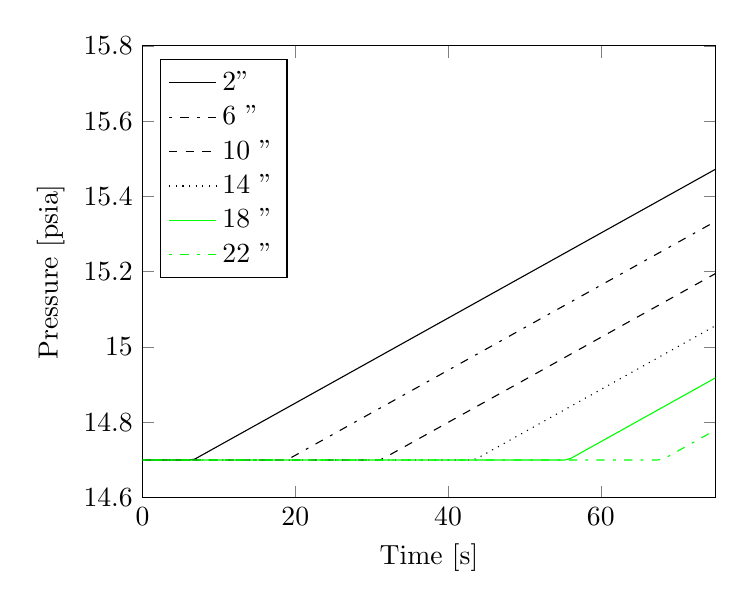
\begin{tikzpicture}

\begin{axis}[%
width=0.6\textwidth,
height=0.473225806451613\textwidth,
scale only axis,
xmin=0,
xmax=75,
xlabel={Time [s]},
ymin=14.6,
ymax=15.8,
ylabel={Pressure [psia]},
legend style={at={(0.03,0.97)},anchor=north west,draw=black,fill=white,legend cell align=left}
]
\addplot [
color=black,
solid
]
table[row sep=crcr]{
0 14.7\\
0.757575757575758 14.7\\
1.51515151515152 14.7\\
2.27272727272727 14.7\\
3.03030303030303 14.7\\
3.78787878787879 14.7\\
4.54545454545455 14.7\\
5.3030303030303 14.7\\
6.06060606060606 14.7\\
6.81818181818182 14.7020837110659\\
7.57575757575758 14.7106386353083\\
8.33333333333333 14.7191935595507\\
9.09090909090909 14.7277484837931\\
9.84848484848485 14.7363034080356\\
10.6060606060606 14.744858332278\\
11.3636363636364 14.7534132565204\\
12.1212121212121 14.7619681807628\\
12.8787878787879 14.7705231050053\\
13.6363636363636 14.7790780292477\\
14.3939393939394 14.7876329534901\\
15.1515151515152 14.7961878777325\\
15.9090909090909 14.804742801975\\
16.6666666666667 14.8132977262174\\
17.4242424242424 14.8218526504598\\
18.1818181818182 14.8304075747022\\
18.9393939393939 14.8389624989447\\
19.6969696969697 14.8475174231871\\
20.4545454545455 14.8560723474295\\
21.2121212121212 14.8646272716719\\
21.969696969697 14.8731821959144\\
22.7272727272727 14.8817371201568\\
23.4848484848485 14.8902920443992\\
24.2424242424242 14.8988469686416\\
25 14.9074018928841\\
25.7575757575758 14.9159568171265\\
26.5151515151515 14.9245117413689\\
27.2727272727273 14.9330666656113\\
28.030303030303 14.9416215898538\\
28.7878787878788 14.9501765140962\\
29.5454545454545 14.9587314383386\\
30.3030303030303 14.967286362581\\
31.0606060606061 14.9758412868234\\
31.8181818181818 14.9843962110659\\
32.5757575757576 14.9929511353083\\
33.3333333333333 15.0015060595507\\
34.0909090909091 15.0100609837931\\
34.8484848484849 15.0186159080356\\
35.6060606060606 15.027170832278\\
36.3636363636364 15.0357257565204\\
37.1212121212121 15.0442806807628\\
37.8787878787879 15.0528356050053\\
38.6363636363636 15.0613905292477\\
39.3939393939394 15.0699454534901\\
40.1515151515151 15.0785003777325\\
40.9090909090909 15.087055301975\\
41.6666666666667 15.0956102262174\\
42.4242424242424 15.1041651504598\\
43.1818181818182 15.1127200747022\\
43.9393939393939 15.1212749989447\\
44.6969696969697 15.1298299231871\\
45.4545454545455 15.1383848474295\\
46.2121212121212 15.1469397716719\\
46.969696969697 15.1554946959144\\
47.7272727272727 15.1640496201568\\
48.4848484848485 15.1726045443992\\
49.2424242424242 15.1811594686416\\
50 15.1897143928841\\
50.7575757575758 15.1982693171265\\
51.5151515151515 15.2068242413689\\
52.2727272727273 15.2153791656113\\
53.030303030303 15.2239340898538\\
53.7878787878788 15.2324890140962\\
54.5454545454545 15.2410439383386\\
55.3030303030303 15.249598862581\\
56.0606060606061 15.2581537868234\\
56.8181818181818 15.2667087110659\\
57.5757575757576 15.2752636353083\\
58.3333333333333 15.2838185595507\\
59.0909090909091 15.2923734837931\\
59.8484848484849 15.3009284080356\\
60.6060606060606 15.309483332278\\
61.3636363636364 15.3180382565204\\
62.1212121212121 15.3265931807628\\
62.8787878787879 15.3351481050053\\
63.6363636363636 15.3437030292477\\
64.3939393939394 15.3522579534901\\
65.1515151515152 15.3608128777325\\
65.9090909090909 15.369367801975\\
66.6666666666667 15.3779227262174\\
67.4242424242424 15.3864776504598\\
68.1818181818182 15.3950325747022\\
68.9393939393939 15.4035874989447\\
69.6969696969697 15.4121424231871\\
70.4545454545455 15.4206973474295\\
71.2121212121212 15.4292522716719\\
71.969696969697 15.4378071959144\\
72.7272727272727 15.4463621201568\\
73.4848484848485 15.4549170443992\\
74.2424242424242 15.4634719686416\\
75 15.4720268928841\\
};
\addlegendentry{2"};

\addplot [
color=black,
dash pattern=on 1pt off 3pt on 3pt off 3pt
]
table[row sep=crcr]{
0 14.7\\
0.757575757575758 14.7\\
1.51515151515152 14.7\\
2.27272727272727 14.7\\
3.03030303030303 14.7\\
3.78787878787879 14.7\\
4.54545454545455 14.7\\
5.3030303030303 14.7\\
6.06060606060606 14.7\\
6.81818181818182 14.7\\
7.57575757575758 14.7\\
8.33333333333333 14.7\\
9.09090909090909 14.7\\
9.84848484848485 14.7\\
10.6060606060606 14.7\\
11.3636363636364 14.7\\
12.1212121212121 14.7\\
12.8787878787879 14.7\\
13.6363636363636 14.7\\
14.3939393939394 14.7\\
15.1515151515152 14.7\\
15.9090909090909 14.7\\
16.6666666666667 14.7\\
17.4242424242424 14.7\\
18.1818181818182 14.7\\
18.9393939393939 14.7004337847128\\
19.6969696969697 14.7089887089552\\
20.4545454545455 14.7175436331976\\
21.2121212121212 14.72609855744\\
21.969696969697 14.7346534816825\\
22.7272727272727 14.7432084059249\\
23.4848484848485 14.7517633301673\\
24.2424242424242 14.7603182544097\\
25 14.7688731786522\\
25.7575757575758 14.7774281028946\\
26.5151515151515 14.785983027137\\
27.2727272727273 14.7945379513794\\
28.030303030303 14.8030928756219\\
28.7878787878788 14.8116477998643\\
29.5454545454545 14.8202027241067\\
30.3030303030303 14.8287576483491\\
31.0606060606061 14.8373125725916\\
31.8181818181818 14.845867496834\\
32.5757575757576 14.8544224210764\\
33.3333333333333 14.8629773453188\\
34.0909090909091 14.8715322695613\\
34.8484848484849 14.8800871938037\\
35.6060606060606 14.8886421180461\\
36.3636363636364 14.8971970422885\\
37.1212121212121 14.905751966531\\
37.8787878787879 14.9143068907734\\
38.6363636363636 14.9228618150158\\
39.3939393939394 14.9314167392582\\
40.1515151515151 14.9399716635007\\
40.9090909090909 14.9485265877431\\
41.6666666666667 14.9570815119855\\
42.4242424242424 14.9656364362279\\
43.1818181818182 14.9741913604704\\
43.9393939393939 14.9827462847128\\
44.6969696969697 14.9913012089552\\
45.4545454545455 14.9998561331976\\
46.2121212121212 15.0084110574401\\
46.969696969697 15.0169659816825\\
47.7272727272727 15.0255209059249\\
48.4848484848485 15.0340758301673\\
49.2424242424242 15.0426307544097\\
50 15.0511856786522\\
50.7575757575758 15.0597406028946\\
51.5151515151515 15.068295527137\\
52.2727272727273 15.0768504513794\\
53.030303030303 15.0854053756219\\
53.7878787878788 15.0939602998643\\
54.5454545454545 15.1025152241067\\
55.3030303030303 15.1110701483491\\
56.0606060606061 15.1196250725916\\
56.8181818181818 15.128179996834\\
57.5757575757576 15.1367349210764\\
58.3333333333333 15.1452898453188\\
59.0909090909091 15.1538447695613\\
59.8484848484849 15.1623996938037\\
60.6060606060606 15.1709546180461\\
61.3636363636364 15.1795095422885\\
62.1212121212121 15.188064466531\\
62.8787878787879 15.1966193907734\\
63.6363636363636 15.2051743150158\\
64.3939393939394 15.2137292392582\\
65.1515151515152 15.2222841635007\\
65.9090909090909 15.2308390877431\\
66.6666666666667 15.2393940119855\\
67.4242424242424 15.2479489362279\\
68.1818181818182 15.2565038604704\\
68.9393939393939 15.2650587847128\\
69.6969696969697 15.2736137089552\\
70.4545454545455 15.2821686331976\\
71.2121212121212 15.2907235574401\\
71.969696969697 15.2992784816825\\
72.7272727272727 15.3078334059249\\
73.4848484848485 15.3163883301673\\
74.2424242424242 15.3249432544097\\
75 15.3334981786522\\
};
\addlegendentry{6 "};

\addplot [
color=black,
dashed
]
table[row sep=crcr]{
0 14.7\\
0.757575757575758 14.7\\
1.51515151515152 14.7\\
2.27272727272727 14.7\\
3.03030303030303 14.7\\
3.78787878787879 14.7\\
4.54545454545455 14.7\\
5.3030303030303 14.7\\
6.06060606060606 14.7\\
6.81818181818182 14.7\\
7.57575757575758 14.7\\
8.33333333333333 14.7\\
9.09090909090909 14.7\\
9.84848484848485 14.7\\
10.6060606060606 14.7\\
11.3636363636364 14.7\\
12.1212121212121 14.7\\
12.8787878787879 14.7\\
13.6363636363636 14.7\\
14.3939393939394 14.7\\
15.1515151515152 14.7\\
15.9090909090909 14.7\\
16.6666666666667 14.7\\
17.4242424242424 14.7\\
18.1818181818182 14.7\\
18.9393939393939 14.7\\
19.6969696969697 14.7\\
20.4545454545455 14.7\\
21.2121212121212 14.7\\
21.969696969697 14.7\\
22.7272727272727 14.7\\
23.4848484848485 14.7\\
24.2424242424242 14.7\\
25 14.7\\
25.7575757575758 14.7\\
26.5151515151515 14.7\\
27.2727272727273 14.7\\
28.030303030303 14.7\\
28.7878787878788 14.7\\
29.5454545454545 14.7\\
30.3030303030303 14.7\\
31.0606060606061 14.7\\
31.8181818181818 14.7073387826021\\
32.5757575757576 14.7158937068445\\
33.3333333333333 14.724448631087\\
34.0909090909091 14.7330035553294\\
34.8484848484849 14.7415584795718\\
35.6060606060606 14.7501134038142\\
36.3636363636364 14.7586683280566\\
37.1212121212121 14.7672232522991\\
37.8787878787879 14.7757781765415\\
38.6363636363636 14.7843331007839\\
39.3939393939394 14.7928880250263\\
40.1515151515151 14.8014429492688\\
40.9090909090909 14.8099978735112\\
41.6666666666667 14.8185527977536\\
42.4242424242424 14.827107721996\\
43.1818181818182 14.8356626462385\\
43.9393939393939 14.8442175704809\\
44.6969696969697 14.8527724947233\\
45.4545454545455 14.8613274189657\\
46.2121212121212 14.8698823432082\\
46.969696969697 14.8784372674506\\
47.7272727272727 14.886992191693\\
48.4848484848485 14.8955471159354\\
49.2424242424242 14.9041020401779\\
50 14.9126569644203\\
50.7575757575758 14.9212118886627\\
51.5151515151515 14.9297668129051\\
52.2727272727273 14.9383217371476\\
53.030303030303 14.94687666139\\
53.7878787878788 14.9554315856324\\
54.5454545454545 14.9639865098748\\
55.3030303030303 14.9725414341173\\
56.0606060606061 14.9810963583597\\
56.8181818181818 14.9896512826021\\
57.5757575757576 14.9982062068445\\
58.3333333333333 15.006761131087\\
59.0909090909091 15.0153160553294\\
59.8484848484849 15.0238709795718\\
60.6060606060606 15.0324259038142\\
61.3636363636364 15.0409808280566\\
62.1212121212121 15.0495357522991\\
62.8787878787879 15.0580906765415\\
63.6363636363636 15.0666456007839\\
64.3939393939394 15.0752005250263\\
65.1515151515152 15.0837554492688\\
65.9090909090909 15.0923103735112\\
66.6666666666667 15.1008652977536\\
67.4242424242424 15.109420221996\\
68.1818181818182 15.1179751462385\\
68.9393939393939 15.1265300704809\\
69.6969696969697 15.1350849947233\\
70.4545454545455 15.1436399189657\\
71.2121212121212 15.1521948432082\\
71.969696969697 15.1607497674506\\
72.7272727272727 15.169304691693\\
73.4848484848485 15.1778596159354\\
74.2424242424242 15.1864145401779\\
75 15.1949694644203\\
};
\addlegendentry{10 "};

\addplot [
color=black,
dotted
]
table[row sep=crcr]{
0 14.7\\
0.757575757575758 14.7\\
1.51515151515152 14.7\\
2.27272727272727 14.7\\
3.03030303030303 14.7\\
3.78787878787879 14.7\\
4.54545454545455 14.7\\
5.3030303030303 14.7\\
6.06060606060606 14.7\\
6.81818181818182 14.7\\
7.57575757575758 14.7\\
8.33333333333333 14.7\\
9.09090909090909 14.7\\
9.84848484848485 14.7\\
10.6060606060606 14.7\\
11.3636363636364 14.7\\
12.1212121212121 14.7\\
12.8787878787879 14.7\\
13.6363636363636 14.7\\
14.3939393939394 14.7\\
15.1515151515152 14.7\\
15.9090909090909 14.7\\
16.6666666666667 14.7\\
17.4242424242424 14.7\\
18.1818181818182 14.7\\
18.9393939393939 14.7\\
19.6969696969697 14.7\\
20.4545454545455 14.7\\
21.2121212121212 14.7\\
21.969696969697 14.7\\
22.7272727272727 14.7\\
23.4848484848485 14.7\\
24.2424242424242 14.7\\
25 14.7\\
25.7575757575758 14.7\\
26.5151515151515 14.7\\
27.2727272727273 14.7\\
28.030303030303 14.7\\
28.7878787878788 14.7\\
29.5454545454545 14.7\\
30.3030303030303 14.7\\
31.0606060606061 14.7\\
31.8181818181818 14.7\\
32.5757575757576 14.7\\
33.3333333333333 14.7\\
34.0909090909091 14.7\\
34.8484848484849 14.7\\
35.6060606060606 14.7\\
36.3636363636364 14.7\\
37.1212121212121 14.7\\
37.8787878787879 14.7\\
38.6363636363636 14.7\\
39.3939393939394 14.7\\
40.1515151515151 14.7\\
40.9090909090909 14.7\\
41.6666666666667 14.7\\
42.4242424242424 14.7\\
43.1818181818182 14.7\\
43.9393939393939 14.705688856249\\
44.6969696969697 14.7142437804914\\
45.4545454545455 14.7227987047339\\
46.2121212121212 14.7313536289763\\
46.969696969697 14.7399085532187\\
47.7272727272727 14.7484634774611\\
48.4848484848485 14.7570184017035\\
49.2424242424242 14.765573325946\\
50 14.7741282501884\\
50.7575757575758 14.7826831744308\\
51.5151515151515 14.7912380986732\\
52.2727272727273 14.7997930229157\\
53.030303030303 14.8083479471581\\
53.7878787878788 14.8169028714005\\
54.5454545454545 14.8254577956429\\
55.3030303030303 14.8340127198854\\
56.0606060606061 14.8425676441278\\
56.8181818181818 14.8511225683702\\
57.5757575757576 14.8596774926126\\
58.3333333333333 14.8682324168551\\
59.0909090909091 14.8767873410975\\
59.8484848484849 14.8853422653399\\
60.6060606060606 14.8938971895823\\
61.3636363636364 14.9024521138248\\
62.1212121212121 14.9110070380672\\
62.8787878787879 14.9195619623096\\
63.6363636363636 14.928116886552\\
64.3939393939394 14.9366718107945\\
65.1515151515152 14.9452267350369\\
65.9090909090909 14.9537816592793\\
66.6666666666667 14.9623365835217\\
67.4242424242424 14.9708915077642\\
68.1818181818182 14.9794464320066\\
68.9393939393939 14.988001356249\\
69.6969696969697 14.9965562804914\\
70.4545454545455 15.0051112047339\\
71.2121212121212 15.0136661289763\\
71.969696969697 15.0222210532187\\
72.7272727272727 15.0307759774611\\
73.4848484848485 15.0393309017036\\
74.2424242424242 15.047885825946\\
75 15.0564407501884\\
};
\addlegendentry{14 "};

\addplot [
color=green,
solid
]
table[row sep=crcr]{
0 14.7\\
0.757575757575758 14.7\\
1.51515151515152 14.7\\
2.27272727272727 14.7\\
3.03030303030303 14.7\\
3.78787878787879 14.7\\
4.54545454545455 14.7\\
5.3030303030303 14.7\\
6.06060606060606 14.7\\
6.81818181818182 14.7\\
7.57575757575758 14.7\\
8.33333333333333 14.7\\
9.09090909090909 14.7\\
9.84848484848485 14.7\\
10.6060606060606 14.7\\
11.3636363636364 14.7\\
12.1212121212121 14.7\\
12.8787878787879 14.7\\
13.6363636363636 14.7\\
14.3939393939394 14.7\\
15.1515151515152 14.7\\
15.9090909090909 14.7\\
16.6666666666667 14.7\\
17.4242424242424 14.7\\
18.1818181818182 14.7\\
18.9393939393939 14.7\\
19.6969696969697 14.7\\
20.4545454545455 14.7\\
21.2121212121212 14.7\\
21.969696969697 14.7\\
22.7272727272727 14.7\\
23.4848484848485 14.7\\
24.2424242424242 14.7\\
25 14.7\\
25.7575757575758 14.7\\
26.5151515151515 14.7\\
27.2727272727273 14.7\\
28.030303030303 14.7\\
28.7878787878788 14.7\\
29.5454545454545 14.7\\
30.3030303030303 14.7\\
31.0606060606061 14.7\\
31.8181818181818 14.7\\
32.5757575757576 14.7\\
33.3333333333333 14.7\\
34.0909090909091 14.7\\
34.8484848484849 14.7\\
35.6060606060606 14.7\\
36.3636363636364 14.7\\
37.1212121212121 14.7\\
37.8787878787879 14.7\\
38.6363636363636 14.7\\
39.3939393939394 14.7\\
40.1515151515151 14.7\\
40.9090909090909 14.7\\
41.6666666666667 14.7\\
42.4242424242424 14.7\\
43.1818181818182 14.7\\
43.9393939393939 14.7\\
44.6969696969697 14.7\\
45.4545454545455 14.7\\
46.2121212121212 14.7\\
46.969696969697 14.7\\
47.7272727272727 14.7\\
48.4848484848485 14.7\\
49.2424242424242 14.7\\
50 14.7\\
50.7575757575758 14.7\\
51.5151515151515 14.7\\
52.2727272727273 14.7\\
53.030303030303 14.7\\
53.7878787878788 14.7\\
54.5454545454545 14.7\\
55.3030303030303 14.7\\
56.0606060606061 14.7040389298959\\
56.8181818181818 14.7125938541383\\
57.5757575757576 14.7211487783808\\
58.3333333333333 14.7297037026232\\
59.0909090909091 14.7382586268656\\
59.8484848484849 14.746813551108\\
60.6060606060606 14.7553684753505\\
61.3636363636364 14.7639233995929\\
62.1212121212121 14.7724783238353\\
62.8787878787879 14.7810332480777\\
63.6363636363636 14.7895881723201\\
64.3939393939394 14.7981430965626\\
65.1515151515152 14.806698020805\\
65.9090909090909 14.8152529450474\\
66.6666666666667 14.8238078692898\\
67.4242424242424 14.8323627935323\\
68.1818181818182 14.8409177177747\\
68.9393939393939 14.8494726420171\\
69.6969696969697 14.8580275662595\\
70.4545454545455 14.866582490502\\
71.2121212121212 14.8751374147444\\
71.969696969697 14.8836923389868\\
72.7272727272727 14.8922472632292\\
73.4848484848485 14.9008021874717\\
74.2424242424242 14.9093571117141\\
75 14.9179120359565\\
};
\addlegendentry{18 "};

\addplot [
color=green,
dash pattern=on 1pt off 3pt on 3pt off 3pt
]
table[row sep=crcr]{
0 14.7\\
0.757575757575758 14.7\\
1.51515151515152 14.7\\
2.27272727272727 14.7\\
3.03030303030303 14.7\\
3.78787878787879 14.7\\
4.54545454545455 14.7\\
5.3030303030303 14.7\\
6.06060606060606 14.7\\
6.81818181818182 14.7\\
7.57575757575758 14.7\\
8.33333333333333 14.7\\
9.09090909090909 14.7\\
9.84848484848485 14.7\\
10.6060606060606 14.7\\
11.3636363636364 14.7\\
12.1212121212121 14.7\\
12.8787878787879 14.7\\
13.6363636363636 14.7\\
14.3939393939394 14.7\\
15.1515151515152 14.7\\
15.9090909090909 14.7\\
16.6666666666667 14.7\\
17.4242424242424 14.7\\
18.1818181818182 14.7\\
18.9393939393939 14.7\\
19.6969696969697 14.7\\
20.4545454545455 14.7\\
21.2121212121212 14.7\\
21.969696969697 14.7\\
22.7272727272727 14.7\\
23.4848484848485 14.7\\
24.2424242424242 14.7\\
25 14.7\\
25.7575757575758 14.7\\
26.5151515151515 14.7\\
27.2727272727273 14.7\\
28.030303030303 14.7\\
28.7878787878788 14.7\\
29.5454545454545 14.7\\
30.3030303030303 14.7\\
31.0606060606061 14.7\\
31.8181818181818 14.7\\
32.5757575757576 14.7\\
33.3333333333333 14.7\\
34.0909090909091 14.7\\
34.8484848484849 14.7\\
35.6060606060606 14.7\\
36.3636363636364 14.7\\
37.1212121212121 14.7\\
37.8787878787879 14.7\\
38.6363636363636 14.7\\
39.3939393939394 14.7\\
40.1515151515151 14.7\\
40.9090909090909 14.7\\
41.6666666666667 14.7\\
42.4242424242424 14.7\\
43.1818181818182 14.7\\
43.9393939393939 14.7\\
44.6969696969697 14.7\\
45.4545454545455 14.7\\
46.2121212121212 14.7\\
46.969696969697 14.7\\
47.7272727272727 14.7\\
48.4848484848485 14.7\\
49.2424242424242 14.7\\
50 14.7\\
50.7575757575758 14.7\\
51.5151515151515 14.7\\
52.2727272727273 14.7\\
53.030303030303 14.7\\
53.7878787878788 14.7\\
54.5454545454545 14.7\\
55.3030303030303 14.7\\
56.0606060606061 14.7\\
56.8181818181818 14.7\\
57.5757575757576 14.7\\
58.3333333333333 14.7\\
59.0909090909091 14.7\\
59.8484848484849 14.7\\
60.6060606060606 14.7\\
61.3636363636364 14.7\\
62.1212121212121 14.7\\
62.8787878787879 14.7\\
63.6363636363636 14.7\\
64.3939393939394 14.7\\
65.1515151515152 14.7\\
65.9090909090909 14.7\\
66.6666666666667 14.7\\
67.4242424242424 14.7\\
68.1818181818182 14.7023890035428\\
68.9393939393939 14.7109439277852\\
69.6969696969697 14.7194988520277\\
70.4545454545455 14.7280537762701\\
71.2121212121212 14.7366087005125\\
71.969696969697 14.7451636247549\\
72.7272727272727 14.7537185489974\\
73.4848484848485 14.7622734732398\\
74.2424242424242 14.7708283974822\\
75 14.7793833217246\\
};
\addlegendentry{22 "};

\end{axis}
\end{tikzpicture}%
\caption{Analytic solution to the filling problem.}
\label{fig:vmpAnalyticSol}
\end{figure}

\tab{tab:vmpLinRunTime} shows the run time data for the linear cases that were run.

\begin{table}[ht]
\centering
\singlespace
\pgfplotstabletypeset[sci zerofill,sci E, col sep=comma,
	columns/0/.style={ column name= $[ \text{s} ]$, precision=1},
	columns/1/.style={ column name= $[ - ]$, int detect},
	columns/2/.style={ column name= $[ \text{s} ]$, precision=3},
	columns/3/.style={ column name= $[ \text{s} ]$, precision=3},
	every head row/.style={
		before row={
			\toprule
			\dtmax{} & $N_{t}$ & $T_{\text{CPU}}$& $\frac{T_{\text{CPU}}}{N_{t}}$\\
		},
		after row=\midrule
	},
	every last row/.style={
after row=\bottomrule}]{tables/vmpLinRunData.tex}
\caption{Linear solver's data for the fill problem.}
\label{tab:vmpLinRunTime}
\end{table}

With the nonlinear solver active, the same three timestep sizes were run.
The pressures from the \dtmax{} = \expneg{1.0}{1}{[s]} case is shown in \fig{fig:nlnFill1em1}.
The measure of error, $e_{p}$, for this simulation was \expneg{3.5}{2}{[s]}.
This error measure was half that of the linear case at the same \dtmax{}.

\begin{figure}[h!t]
\centering
% This file was created by matlab2tikz v0.4.3.
% Copyright (c) 2008--2013, Nico Schlömer <nico.schloemer@gmail.com>
% All rights reserved.
% 
\tikzsetnextfilename{plots/vmpNLN1em1_eps}
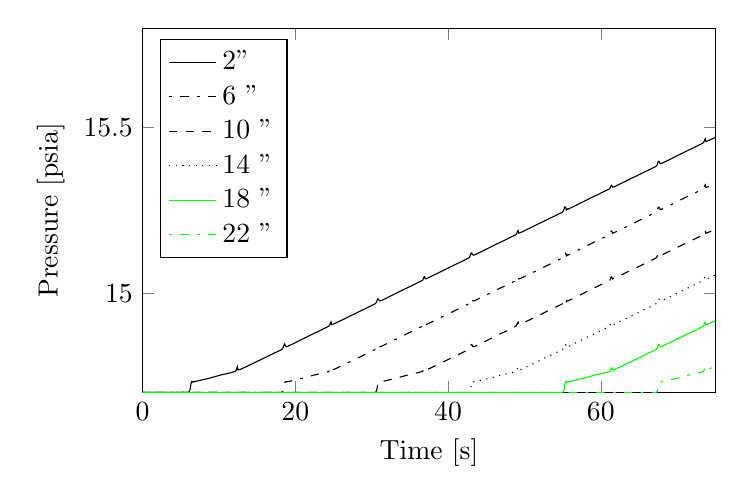
\begin{tikzpicture}

\begin{axis}[%
width=0.6\textwidth,
height=0.381611494576701\textwidth,
scale only axis,
xmin=0,
xmax=75,
xlabel={Time [s]},
ymin=14.7,
ymax=15.8,
ylabel={Pressure [psia]},
legend style={at={(0.03,0.97)},anchor=north west,draw=black,fill=white,legend cell align=left}
]
\addplot [
color=black,
solid
]
table[row sep=crcr]{
0 14.7007818222046\\
9.99999971718069e-10 14.7007818222046\\
2.49999998480632e-09 14.7007818222046\\
4.74999994892755e-09 14.7007818222046\\
8.1250002281763e-09 14.7007818222046\\
1.31874999809156e-08 14.7007818222046\\
2.0781250498203e-08 14.7007818222046\\
3.21718758300449e-08 14.7007818222046\\
4.92578138278077e-08 14.7007818222046\\
7.48867208244519e-08 14.7007818222046\\
1.13330081319418e-07 14.7007818222046\\
1.70995122061868e-07 14.7007818222046\\
2.57492672517401e-07 14.7007818222046\\
3.8723902662241e-07 14.7007818222046\\
5.81858500936505e-07 14.7007818222046\\
8.73787769251066e-07 14.7007818222046\\
1.31168167172291e-06 14.7007818222046\\
1.9685226106958e-06 14.7007827758789\\
2.95378367809462e-06 14.7007827758789\\
4.43167573394021e-06 14.7007827758789\\
6.64851359033491e-06 14.7007827758789\\
9.97376992017962e-06 14.7007837295532\\
1.49616553244414e-05 14.7007846832275\\
2.24434825213393e-05 14.7007856369019\\
3.36662233166862e-05 14.7007865905762\\
5.05003372381907e-05 14.7007884979248\\
7.57515081204474e-05 14.7007904052734\\
0.000113628258986864 14.7007932662964\\
0.000170443381648511 14.700795173645\\
0.000255666091106832 14.7007970809937\\
0.000383500126190484 14.7007970809937\\
0.000575251178815961 14.7007942199707\\
0.000862877757754177 14.7007904052734\\
0.00129431765526533 14.7007865905762\\
0.00194147753063589 14.7007837295532\\
0.00291221728548408 14.700779914856\\
0.00436832662671804 14.7007780075073\\
0.00597004732117057 14.700779914856\\
0.00773194013163447 14.7007827758789\\
0.009670021943748 14.7007837295532\\
0.0118019115179777 14.7007827758789\\
0.0141469910740852 14.7007827758789\\
0.0167265776544809 14.7007827758789\\
0.0195641238242388 14.7007827758789\\
0.0226854234933853 14.7007827758789\\
0.0261188540607691 14.7007827758789\\
0.0298956278711557 14.7007827758789\\
0.0340500771999359 14.7007827758789\\
0.0386199727654457 14.7007827758789\\
0.0436468608677387 14.7007827758789\\
0.0491764321923256 14.7007827758789\\
0.0552589632570744 14.7007827758789\\
0.0619497485458851 14.7007827758789\\
0.0693096145987511 14.7007827758789\\
0.0774054601788521 14.700777053833\\
0.0863108932971954 14.7007865905762\\
0.0961068719625473 14.7007827758789\\
0.106882445514202 14.7007827758789\\
0.118735581636429 14.7007827758789\\
0.13177402317524 14.7007827758789\\
0.146116316318512 14.7007827758789\\
0.161892831325531 14.7007827758789\\
0.179247006773949 14.7007827758789\\
0.198336601257324 14.7007827758789\\
0.21933513879776 14.7007827758789\\
0.242433547973633 14.7007827758789\\
0.267841786146164 14.7007827758789\\
0.29579085111618 14.7007827758789\\
0.32653483748436 14.7007827758789\\
0.360353201627731 14.7007827758789\\
0.397553414106369 14.7007837295532\\
0.438473641872406 14.7007837295532\\
0.483485877513886 14.7007837295532\\
0.532999336719513 14.7007837295532\\
0.587464153766632 14.7007837295532\\
0.647375464439392 14.7007837295532\\
0.71327793598175 14.7007837295532\\
0.7857705950737 14.7007837295532\\
0.865512549877167 14.7007837295532\\
0.953228712081909 14.7007837295532\\
1.04971647262573 14.7007837295532\\
1.14971649646759 14.7007827758789\\
1.24971640110016 14.7007827758789\\
1.34971642494202 14.7007827758789\\
1.44971644878387 14.7007827758789\\
1.54971647262573 14.7007827758789\\
1.64971649646759 14.7007827758789\\
1.74971640110016 14.7007827758789\\
1.84971642494202 14.7007827758789\\
1.94971644878387 14.7007827758789\\
2.04971647262573 14.7007827758789\\
2.1497163772583 14.7007827758789\\
2.24971652030945 14.7007827758789\\
2.34971642494202 14.7007827758789\\
2.44971656799316 14.7007827758789\\
2.54971647262573 14.7007827758789\\
2.6497163772583 14.7007827758789\\
2.74971652030945 14.7007827758789\\
2.84971642494202 14.7007827758789\\
2.94971656799316 14.7007827758789\\
3.04971647262573 14.7007827758789\\
3.1497163772583 14.7007827758789\\
3.24971652030945 14.7007827758789\\
3.34971642494202 14.7007827758789\\
3.44971656799316 14.7007827758789\\
3.54971647262573 14.7007827758789\\
3.6497163772583 14.7007827758789\\
3.74971652030945 14.7007827758789\\
3.84971642494202 14.7007827758789\\
3.94971656799316 14.7007827758789\\
4.04971647262573 14.7007827758789\\
4.1497163772583 14.7007827758789\\
4.24971628189087 14.7007827758789\\
4.3497166633606 14.7007827758789\\
4.44971656799316 14.7007827758789\\
4.54971647262573 14.7007827758789\\
4.6497163772583 14.7007827758789\\
4.74971628189087 14.7007827758789\\
4.8497166633606 14.7007827758789\\
4.94971656799316 14.7007827758789\\
5.04971647262573 14.7007837295532\\
5.1497163772583 14.7007837295532\\
5.24971628189087 14.7007837295532\\
5.3497166633606 14.7007837295532\\
5.44971656799316 14.7007837295532\\
5.54971647262573 14.7007837295532\\
5.6497163772583 14.7007846832275\\
5.74971628189087 14.7007894515991\\
5.8497166633606 14.7008085250854\\
5.94971656799316 14.7009077072144\\
6.04971647262573 14.7014436721802\\
6.1497163772583 14.7040977478027\\
6.24971628189087 14.7128324508667\\
6.3497166633606 14.7271690368652\\
6.44971656799316 14.7334566116333\\
6.54971647262573 14.7314443588257\\
6.6497163772583 14.7334966659546\\
6.74971628189087 14.7322854995728\\
6.8497166633606 14.7336616516113\\
6.94971656799316 14.7335815429688\\
7.04971647262573 14.7345237731934\\
7.1497163772583 14.7347774505615\\
7.24971628189087 14.7354955673218\\
7.3497166633606 14.7358999252319\\
7.44971656799316 14.7365169525146\\
7.54971647262573 14.7369899749756\\
7.6497163772583 14.7375602722168\\
7.74971628189087 14.7380647659302\\
7.8497166633606 14.7386140823364\\
7.94971656799316 14.7391328811646\\
8.04971599578857 14.739673614502\\
8.1497163772583 14.7401990890503\\
8.24971675872803 14.7407350540161\\
8.34971618652344 14.7412633895874\\
8.44971656799316 14.7417974472046\\
8.54971599578857 14.7423276901245\\
8.6497163772583 14.7428607940674\\
8.74971675872803 14.7433929443359\\
8.84971618652344 14.7439479827881\\
8.94971656799316 14.7448120117188\\
9.04971599578857 14.7454252243042\\
9.1497163772583 14.7460870742798\\
9.24971675872803 14.7467250823975\\
9.34971618652344 14.7473707199097\\
9.44971656799316 14.748010635376\\
9.54971599578857 14.7486515045166\\
9.6497163772583 14.7492904663086\\
9.74971675872803 14.7499284744263\\
9.84971618652344 14.7505655288696\\
9.94971656799316 14.751202583313\\
10.0497159957886 14.751838684082\\
10.1497163772583 14.7524747848511\\
10.249716758728 14.7531108856201\\
10.3497161865234 14.7537298202515\\
10.4497165679932 14.7540988922119\\
10.5497159957886 14.7545909881592\\
10.6497163772583 14.7551307678223\\
10.749716758728 14.755651473999\\
10.8497161865234 14.7561731338501\\
10.9497165679932 14.756688117981\\
11.0497159957886 14.7571992874146\\
11.1497163772583 14.7577028274536\\
11.249716758728 14.7581987380981\\
11.3497161865234 14.7586870193481\\
11.4497165679932 14.7591991424561\\
11.5497159957886 14.7598543167114\\
11.6497163772583 14.7605504989624\\
11.749716758728 14.7611818313599\\
11.8497161865234 14.7618141174316\\
11.9497165679932 14.7624731063843\\
12.0497159957886 14.7631711959839\\
12.1497163772583 14.7639303207397\\
12.249716758728 14.7665214538574\\
12.3471450805664 14.7732496261597\\
12.4250917434692 14.7781705856323\\
12.4879579544067 14.768609046936\\
12.557110786438 14.7686433792114\\
12.6331787109375 14.7690782546997\\
12.7168531417847 14.7695474624634\\
12.808895111084 14.7702302932739\\
12.9088954925537 14.7711057662964\\
13.0088949203491 14.7721309661865\\
13.1088953018188 14.7731733322144\\
13.2088947296143 14.7742366790771\\
13.308895111084 14.7753143310547\\
13.4088954925537 14.7763986587524\\
13.5088949203491 14.777494430542\\
13.6088953018188 14.7785978317261\\
13.7088947296143 14.7797069549561\\
13.808895111084 14.780816078186\\
13.9088954925537 14.781925201416\\
14.0088949203491 14.783034324646\\
14.1088953018188 14.784143447876\\
14.2088947296143 14.7852535247803\\
14.308895111084 14.7863636016846\\
14.4088954925537 14.7874736785889\\
14.5088949203491 14.7885837554932\\
14.6088953018188 14.7896947860718\\
14.7088947296143 14.7908058166504\\
14.808895111084 14.7919178009033\\
14.9088954925537 14.7930297851563\\
15.0088949203491 14.7941417694092\\
15.1088953018188 14.7952537536621\\
15.2088947296143 14.7963666915894\\
15.308895111084 14.7974805831909\\
15.4088954925537 14.7986001968384\\
15.5088949203491 14.7997035980225\\
15.6088953018188 14.8008260726929\\
15.7088947296143 14.8019437789917\\
15.808895111084 14.8030633926392\\
15.9088954925537 14.8041830062866\\
16.0088958740234 14.8053026199341\\
16.1088943481445 14.8064222335815\\
16.2088947296143 14.8075428009033\\
16.308895111084 14.8086624145508\\
16.4088954925537 14.8097829818726\\
16.5088958740234 14.8109035491943\\
16.6088943481445 14.8120241165161\\
16.7088947296143 14.8131446838379\\
16.808895111084 14.814266204834\\
16.9088954925537 14.8153867721558\\
17.0088958740234 14.8165082931519\\
17.1088943481445 14.8176298141479\\
17.2088947296143 14.818751335144\\
17.308895111084 14.8198738098145\\
17.4088954925537 14.8209953308105\\
17.5088958740234 14.822117805481\\
17.6088943481445 14.8232402801514\\
17.7088947296143 14.8243627548218\\
17.808895111084 14.8254852294922\\
17.9088954925537 14.8266096115112\\
18.0088958740234 14.8277368545532\\
18.1088943481445 14.8288841247559\\
18.2088947296143 14.830132484436\\
18.308895111084 14.8319272994995\\
18.4088954925537 14.8359346389771\\
18.5088958740234 14.8431234359741\\
18.6088943481445 14.8468885421753\\
18.7088947296143 14.8412246704102\\
18.808895111084 14.8385257720947\\
18.9088954925537 14.8396024703979\\
19.0088958740234 14.8392372131348\\
19.1088943481445 14.8409767150879\\
19.2088947296143 14.8416633605957\\
19.308895111084 14.8430795669556\\
19.4088954925537 14.8440103530884\\
19.5088958740234 14.8452653884888\\
19.6088943481445 14.8463039398193\\
19.7088947296143 14.8474884033203\\
19.808895111084 14.848575592041\\
19.9088954925537 14.8497276306152\\
20.0088958740234 14.8508358001709\\
20.1088943481445 14.8519744873047\\
20.2088947296143 14.8530921936035\\
20.308895111084 14.8542242050171\\
20.4088954925537 14.8553476333618\\
20.5088958740234 14.8564767837524\\
20.6088943481445 14.8576021194458\\
20.7088947296143 14.8587303161621\\
20.808895111084 14.8598566055298\\
20.9088954925537 14.8609848022461\\
21.0088958740234 14.8621110916138\\
21.1088943481445 14.8633079528809\\
21.2088947296143 14.8647031784058\\
21.308895111084 14.8657855987549\\
21.4088954925537 14.8669328689575\\
21.5088958740234 14.8680543899536\\
21.6088943481445 14.8691864013672\\
21.7088947296143 14.8703145980835\\
21.808895111084 14.8714447021484\\
21.9088954925537 14.8725738525391\\
22.0088958740234 14.8737049102783\\
22.1088943481445 14.8748359680176\\
22.2088947296143 14.8759670257568\\
22.308895111084 14.8770990371704\\
22.4088954925537 14.878231048584\\
22.5088958740234 14.8793640136719\\
22.6088943481445 14.8804807662964\\
22.7088947296143 14.8813285827637\\
22.808895111084 14.8824396133423\\
22.9088954925537 14.8835592269897\\
23.0088958740234 14.8846778869629\\
23.1088943481445 14.8857955932617\\
23.2088947296143 14.8869123458862\\
23.308895111084 14.8880281448364\\
23.4088954925537 14.889142036438\\
23.5088958740234 14.8902549743652\\
23.6088943481445 14.8913650512695\\
23.7088947296143 14.8925113677979\\
23.808895111084 14.8937644958496\\
23.9088954925537 14.894998550415\\
24.0088958740234 14.8961601257324\\
24.1088943481445 14.8973197937012\\
24.2088947296143 14.8984975814819\\
24.308895111084 14.8997011184692\\
24.4088954925537 14.9009475708008\\
24.5088958740234 14.9045486450195\\
24.6048831939697 14.910834312439\\
24.681676864624 14.9136018753052\\
24.7464084625244 14.9051694869995\\
24.8176136016846 14.9055252075195\\
24.895938873291 14.9060869216919\\
24.9820976257324 14.9067459106445\\
25.0768718719482 14.9075870513916\\
25.176872253418 14.9086112976074\\
25.2768707275391 14.9097194671631\\
25.3768711090088 14.9108257293701\\
25.4768714904785 14.911937713623\\
25.5768718719482 14.9130535125732\\
25.676872253418 14.9141712188721\\
25.7768707275391 14.9152879714966\\
25.8768711090088 14.9164094924927\\
25.9768714904785 14.9175319671631\\
26.0768718719482 14.9186611175537\\
26.176872253418 14.9197883605957\\
26.2768707275391 14.920916557312\\
26.3768711090088 14.9220447540283\\
26.4768714904785 14.9231729507446\\
26.5768718719482 14.9243001937866\\
26.676872253418 14.9254283905029\\
26.7768707275391 14.9265565872192\\
26.8768711090088 14.9276838302612\\
26.9768714904785 14.9288120269775\\
27.0768718719482 14.9299402236938\\
27.176872253418 14.9310674667358\\
27.2768707275391 14.9321956634521\\
27.3768711090088 14.9333238601685\\
27.4768714904785 14.9344511032104\\
27.5768718719482 14.9355792999268\\
27.676872253418 14.9367065429688\\
27.7768707275391 14.9378347396851\\
27.8768711090088 14.9389629364014\\
27.9768714904785 14.9400901794434\\
28.0768718719482 14.9412183761597\\
28.176872253418 14.9423456192017\\
28.2768707275391 14.9434804916382\\
28.3768711090088 14.9445905685425\\
28.4768714904785 14.9457235336304\\
28.5768718719482 14.946849822998\\
28.676872253418 14.9479780197144\\
28.7768707275391 14.9491062164307\\
28.8768711090088 14.950234413147\\
28.9768714904785 14.9513626098633\\
29.0768718719482 14.9524898529053\\
29.176872253418 14.9536180496216\\
29.2768707275391 14.9547462463379\\
29.3768711090088 14.9558744430542\\
29.4768714904785 14.9570026397705\\
29.5768718719482 14.9581298828125\\
29.676872253418 14.9592580795288\\
29.7768707275391 14.9603862762451\\
29.8768711090088 14.9615144729614\\
29.9768714904785 14.9626426696777\\
30.0768718719482 14.963770866394\\
30.176872253418 14.964900970459\\
30.2768707275391 14.9660387039185\\
30.3768711090088 14.9672107696533\\
30.4768714904785 14.9685831069946\\
30.5768718719482 14.9709510803223\\
30.676872253418 14.9764404296875\\
30.7768707275391 14.9835319519043\\
30.8768711090088 14.9819793701172\\
30.9768714904785 14.9787912368774\\
31.0768718719482 14.9764232635498\\
31.176872253418 14.9774360656738\\
31.2768707275391 14.9776411056519\\
31.3768711090088 14.9792537689209\\
31.4768714904785 14.9800567626953\\
31.5768718719482 14.9814014434814\\
31.676872253418 14.982385635376\\
31.7768707275391 14.9836101531982\\
31.8768711090088 14.9846744537354\\
31.9768714904785 14.9858465194702\\
32.0768699645996 14.986946105957\\
32.176872253418 14.988094329834\\
32.2768707275391 14.9892101287842\\
32.3768730163574 14.9903469085693\\
32.4768714904785 14.9914693832397\\
32.5768699645996 14.9926023483276\\
32.676872253418 14.9937286376953\\
32.7768707275391 14.9948596954346\\
32.8768730163574 14.9959878921509\\
32.9768714904785 14.9971179962158\\
33.0768699645996 14.9982461929321\\
33.176872253418 14.9993753433228\\
33.2768707275391 15.0005044937134\\
33.3768730163574 15.0018339157104\\
33.4768714904785 15.0030736923218\\
33.5768699645996 15.0041904449463\\
33.676872253418 15.0053262710571\\
33.7768707275391 15.0064544677734\\
33.8768730163574 15.0075855255127\\
33.9768714904785 15.0087156295776\\
34.0768699645996 15.0098466873169\\
34.176872253418 15.0109786987305\\
34.2768707275391 15.0121097564697\\
34.3768730163574 15.0132417678833\\
34.4768714904785 15.0143747329712\\
34.5768699645996 15.0155076980591\\
34.676872253418 15.0166416168213\\
34.7768707275391 15.0177755355835\\
34.8768730163574 15.0188503265381\\
34.9768714904785 15.0196676254272\\
35.0768699645996 15.0208778381348\\
35.176872253418 15.0219659805298\\
35.2768707275391 15.0230979919434\\
35.3768730163574 15.0242118835449\\
35.4768714904785 15.0253314971924\\
35.5768699645996 15.0264482498169\\
35.676872253418 15.0275640487671\\
35.7768707275391 15.0286779403687\\
35.8768730163574 15.0297899246216\\
35.9768714904785 15.0309648513794\\
36.0768699645996 15.0322227478027\\
36.176872253418 15.0334167480469\\
36.2768707275391 15.034571647644\\
36.3768730163574 15.0357360839844\\
36.4768714904785 15.036919593811\\
36.5768699645996 15.0381326675415\\
36.676872253418 15.0393943786621\\
36.7768707275391 15.0450391769409\\
36.8673248291016 15.049633026123\\
36.9396858215332 15.0495872497559\\
37.0192794799805 15.043267250061\\
37.1068305969238 15.0439195632935\\
37.2031402587891 15.0445756912231\\
37.3031425476074 15.0454921722412\\
37.4031410217285 15.046555519104\\
37.5031433105469 15.0476732254028\\
37.603141784668 15.0487785339355\\
37.7031402587891 15.0498905181885\\
37.8031425476074 15.0510053634644\\
37.9031410217285 15.0521259307861\\
38.0031433105469 15.053240776062\\
38.103141784668 15.0543622970581\\
38.2031402587891 15.0554847717285\\
38.3031425476074 15.0566120147705\\
38.4031410217285 15.0577402114868\\
38.5031433105469 15.0588684082031\\
38.603141784668 15.0599966049194\\
38.7031402587891 15.0611248016357\\
38.8031425476074 15.0622529983521\\
38.9031410217285 15.0633811950684\\
39.0031433105469 15.064510345459\\
39.103141784668 15.0656385421753\\
39.2031402587891 15.0667667388916\\
39.3031425476074 15.0678939819336\\
39.4031410217285 15.0690221786499\\
39.5031433105469 15.0701503753662\\
39.603141784668 15.0712785720825\\
39.7031402587891 15.0724067687988\\
39.8031425476074 15.0735349655151\\
39.9031410217285 15.0746631622314\\
40.0031433105469 15.0757913589478\\
40.103141784668 15.0769195556641\\
40.2031402587891 15.0780477523804\\
40.3031425476074 15.0791759490967\\
40.4031410217285 15.080304145813\\
40.5031433105469 15.0814323425293\\
40.603141784668 15.0825595855713\\
40.7031402587891 15.0836877822876\\
40.8031425476074 15.0848159790039\\
40.9031410217285 15.0859508514404\\
41.0031433105469 15.0870609283447\\
41.103141784668 15.0881948471069\\
41.2031402587891 15.0893211364746\\
41.3031425476074 15.0904502868652\\
41.4031410217285 15.0915775299072\\
41.5031433105469 15.0927066802979\\
41.603141784668 15.0938348770142\\
41.7031402587891 15.0949630737305\\
41.8031425476074 15.0960912704468\\
41.9031410217285 15.0972194671631\\
42.0031433105469 15.0983476638794\\
42.103141784668 15.0994758605957\\
42.2031402587891 15.100604057312\\
42.3031425476074 15.1017332077026\\
42.4031410217285 15.1028623580933\\
42.5031433105469 15.1039972305298\\
42.603141784668 15.1051588058472\\
42.7031402587891 15.1064653396606\\
42.8031425476074 15.1085252761841\\
42.9031410217285 15.1132879257202\\
43.0031433105469 15.1205997467041\\
43.103141784668 15.1216335296631\\
43.2031402587891 15.1170101165771\\
43.3031425476074 15.1146373748779\\
43.4031410217285 15.1156311035156\\
43.5031433105469 15.1155347824097\\
43.603141784668 15.1172714233398\\
43.7031402587891 15.1179876327515\\
43.8031425476074 15.1193904876709\\
43.9031410217285 15.1203365325928\\
44.0031433105469 15.1215858459473\\
44.103141784668 15.122633934021\\
44.2031402587891 15.1238164901733\\
44.3031425476074 15.1249094009399\\
44.4031410217285 15.1260623931885\\
44.5031433105469 15.1271753311157\\
44.603141784668 15.1283149719238\\
44.7031402587891 15.1294364929199\\
44.8031425476074 15.1305704116821\\
44.9031410217285 15.1316957473755\\
45.0031433105469 15.1328277587891\\
45.103141784668 15.1339550018311\\
45.2031402587891 15.1350860595703\\
45.3031425476074 15.1362142562866\\
45.4031410217285 15.1373443603516\\
45.5031433105469 15.1384735107422\\
45.603141784668 15.1397323608398\\
45.7031402587891 15.1410551071167\\
45.8031425476074 15.1421518325806\\
45.9031410217285 15.1432952880859\\
46.0031433105469 15.1444206237793\\
46.103141784668 15.1455535888672\\
46.2031402587891 15.1466836929321\\
46.3031425476074 15.1478147506714\\
46.4031410217285 15.148946762085\\
46.5031433105469 15.1500787734985\\
46.603141784668 15.1512107849121\\
46.7031402587891 15.15234375\\
46.8031425476074 15.1534767150879\\
46.9031410217285 15.1546106338501\\
47.0031433105469 15.1557445526123\\
47.103141784668 15.1568603515625\\
47.2031402587891 15.1576738357544\\
47.3031425476074 15.1588430404663\\
47.4031410217285 15.1599454879761\\
47.5031433105469 15.1610727310181\\
47.603141784668 15.1621894836426\\
47.7031402587891 15.1633100509644\\
47.8031425476074 15.1644268035889\\
47.9031410217285 15.1655435562134\\
48.0031433105469 15.1666593551636\\
48.103141784668 15.1677732467651\\
48.2031402587891 15.1689252853394\\
48.3031425476074 15.1701631546021\\
48.4031410217285 15.1713724136353\\
48.5031433105469 15.1725301742554\\
48.603141784668 15.1736907958984\\
48.7031402587891 15.1748695373535\\
48.8031425476074 15.1760740280151\\
48.9031410217285 15.1773223876953\\
49.0031433105469 15.1814069747925\\
49.0980262756348 15.1872444152832\\
49.1739387512207 15.1892910003662\\
49.2413482666016 15.1814727783203\\
49.315502166748 15.1819105148315\\
49.3970718383789 15.1824760437012\\
49.4867973327637 15.1831884384155\\
49.5854949951172 15.1840810775757\\
49.6854934692383 15.1851644515991\\
49.7854957580566 15.1862697601318\\
49.8854942321777 15.1873788833618\\
49.9854927062988 15.1884908676147\\
50.0854949951172 15.1896085739136\\
50.1854934692383 15.1907272338867\\
50.2854957580566 15.1918439865112\\
50.3854942321777 15.1929664611816\\
50.4854927062988 15.1940898895264\\
50.5854949951172 15.1952180862427\\
50.6854934692383 15.196346282959\\
50.7854957580566 15.1974744796753\\
50.8854942321777 15.1986026763916\\
50.9854927062988 15.1997308731079\\
51.0854949951172 15.2008600234985\\
51.1854934692383 15.2019882202148\\
51.2854957580566 15.2031164169312\\
51.3854942321777 15.2042446136475\\
51.4854927062988 15.2053728103638\\
51.5854949951172 15.2065010070801\\
51.6854934692383 15.2076292037964\\
51.7854957580566 15.2087574005127\\
51.8854942321777 15.209885597229\\
51.9854927062988 15.2110137939453\\
52.0854949951172 15.2121429443359\\
52.1854934692383 15.2132711410522\\
52.2854957580566 15.2143993377686\\
52.3854942321777 15.2155275344849\\
52.4854927062988 15.2166557312012\\
52.5854949951172 15.2177839279175\\
52.6854934692383 15.2189121246338\\
52.7854957580566 15.2200403213501\\
52.8854942321777 15.2211685180664\\
52.9854927062988 15.2222967147827\\
53.0854949951172 15.223424911499\\
53.1854934692383 15.2245531082153\\
53.2854957580566 15.2256879806519\\
53.3854942321777 15.2267980575562\\
53.4854927062988 15.227931022644\\
53.5854949951172 15.229058265686\\
53.6854934692383 15.2301864624023\\
53.7854957580566 15.2313146591187\\
53.8854942321777 15.2324438095093\\
53.9854927062988 15.2335720062256\\
54.0854949951172 15.2347002029419\\
54.1854934692383 15.2358283996582\\
54.2854957580566 15.2369565963745\\
54.3854942321777 15.2380847930908\\
54.4854927062988 15.2392139434814\\
54.5854949951172 15.2403430938721\\
54.6854934692383 15.241473197937\\
54.7854957580566 15.2426128387451\\
54.8854942321777 15.2437982559204\\
54.9854927062988 15.2452363967896\\
55.0854949951172 15.2478904724121\\
55.1854934692383 15.2539110183716\\
55.2854957580566 15.2606420516968\\
55.3854942321777 15.2597846984863\\
55.4854927062988 15.2512769699097\\
55.5854949951172 15.2546529769897\\
55.6854934692383 15.253002166748\\
55.7854957580566 15.2549076080322\\
55.8854942321777 15.2553720474243\\
55.9854927062988 15.2569379806519\\
56.0854949951172 15.2577753067017\\
56.1854934692383 15.2590970993042\\
56.2854957580566 15.2600975036621\\
56.3854942321777 15.2613115310669\\
56.4854927062988 15.2623834609985\\
56.5854949951172 15.2635507583618\\
56.6854934692383 15.2646541595459\\
56.7854957580566 15.2658004760742\\
56.8854942321777 15.2669172286987\\
56.9854927062988 15.2680540084839\\
57.0854949951172 15.2691783905029\\
57.1854934692383 15.2703104019165\\
57.2854957580566 15.2714376449585\\
57.3854942321777 15.2725687026978\\
57.4854927062988 15.2736968994141\\
57.5854949951172 15.274827003479\\
57.6854934692383 15.2759561538696\\
57.7854957580566 15.2770862579346\\
57.8854942321777 15.2784557342529\\
57.9854927062988 15.2796449661255\\
58.0854949951172 15.2807722091675\\
58.1854934692383 15.2819042205811\\
58.2854957580566 15.283034324646\\
58.3854942321777 15.2841653823853\\
58.4854927062988 15.2852964401245\\
58.5854949951172 15.2864274978638\\
58.6854934692383 15.2875595092773\\
58.7854957580566 15.2886915206909\\
58.8854942321777 15.2898244857788\\
58.9854927062988 15.2909574508667\\
59.0854949951172 15.2920904159546\\
59.1854934692383 15.2932243347168\\
59.2854957580566 15.2943592071533\\
59.3854942321777 15.2953977584839\\
59.4854927062988 15.2962646484375\\
59.5854949951172 15.2974615097046\\
59.6854934692383 15.2985553741455\\
59.7854957580566 15.2996864318848\\
59.8854942321777 15.300802230835\\
59.9427452087402 15.3018217086792\\
60 15.3025913238525\\
60.0629768371582 15.3032102584839\\
60.1322555541992 15.303918838501\\
60.2084579467773 15.3046903610229\\
60.2922821044922 15.3055410385132\\
60.3844909667969 15.3064756393433\\
60.484489440918 15.3075647354126\\
60.5844879150391 15.3087959289551\\
60.6844902038574 15.3099842071533\\
60.7844886779785 15.3111343383789\\
60.8844909667969 15.3123006820679\\
60.984489440918 15.3134851455688\\
61.0844879150391 15.3147001266479\\
61.1844902038574 15.3159656524658\\
61.2844886779785 15.3222026824951\\
61.3734016418457 15.326319694519\\
61.444522857666 15.3252925872803\\
61.5227546691895 15.3197784423828\\
61.6088104248047 15.3204212188721\\
61.7034721374512 15.321081161499\\
61.8034706115723 15.3219861984253\\
61.9034729003906 15.3230514526367\\
62.0034713745117 15.3241662979126\\
62.1034736633301 15.3252716064453\\
62.2034721374512 15.3263835906982\\
62.3034706115723 15.3274984359741\\
62.4034729003906 15.3286180496216\\
62.5034713745117 15.3297338485718\\
62.6034736633301 15.3308553695679\\
62.7034721374512 15.3319787979126\\
62.8034706115723 15.333104133606\\
62.9034729003906 15.3342332839966\\
63.0034713745117 15.3353614807129\\
63.1034736633301 15.3364896774292\\
63.2034721374512 15.3376178741455\\
63.3034706115723 15.3387470245361\\
63.4034729003906 15.3398752212524\\
63.5034713745117 15.3410034179688\\
63.6034736633301 15.3421316146851\\
63.7034721374512 15.3432598114014\\
63.8034706115723 15.3443880081177\\
63.9034729003906 15.3455171585083\\
64.0034713745117 15.3466453552246\\
64.1034698486328 15.3477735519409\\
64.2034759521484 15.3489017486572\\
64.3034744262695 15.3500299453735\\
64.4034729003906 15.3511581420898\\
64.5034713745117 15.3522863388062\\
64.6034698486328 15.3534145355225\\
64.7034759521484 15.3545427322388\\
64.8034744262695 15.3556709289551\\
64.9034729003906 15.3567991256714\\
65.0034713745117 15.3579273223877\\
65.1034698486328 15.359055519104\\
65.2034759521484 15.3601837158203\\
65.3034744262695 15.3613119125366\\
65.4034729003906 15.3624401092529\\
65.5034713745117 15.3635683059692\\
65.6034698486328 15.3646965026855\\
65.7034759521484 15.3658313751221\\
65.8034744262695 15.3669424057007\\
65.9034729003906 15.3680763244629\\
66.0034713745117 15.3692026138306\\
66.1034698486328 15.3703317642212\\
66.2034759521484 15.3714599609375\\
66.3034744262695 15.3725881576538\\
66.4034729003906 15.3737163543701\\
66.5034713745117 15.3748445510864\\
66.6034698486328 15.3759727478027\\
66.7034759521484 15.377100944519\\
66.8034744262695 15.3782300949097\\
66.9034729003906 15.3793601989746\\
67.0034713745117 15.3804950714111\\
67.1034698486328 15.3816547393799\\
67.2034759521484 15.3829555511475\\
67.3034744262695 15.3849878311157\\
67.4034729003906 15.389669418335\\
67.5034713745117 15.3969898223877\\
67.6034698486328 15.3983030319214\\
67.7034759521484 15.3935499191284\\
67.8034744262695 15.3911628723145\\
67.9034729003906 15.3921585083008\\
68.0034713745117 15.3920278549194\\
68.1034698486328 15.3937759399414\\
68.2034759521484 15.3944845199585\\
68.3034744262695 15.3958921432495\\
68.4034729003906 15.3968353271484\\
68.5034713745117 15.3980865478516\\
68.6034698486328 15.399133682251\\
68.7034759521484 15.4003171920776\\
68.8034744262695 15.4014101028442\\
68.9034729003906 15.4025630950928\\
69.0034713745117 15.40367603302\\
69.1034698486328 15.4048156738281\\
69.2034759521484 15.4059371948242\\
69.3034744262695 15.4070711135864\\
69.4034729003906 15.4081974029541\\
69.5034713745117 15.4093284606934\\
69.6034698486328 15.4104566574097\\
69.7034759521484 15.4115867614746\\
69.8034744262695 15.4127159118652\\
69.9034729003906 15.4138460159302\\
70.0034713745117 15.4149751663208\\
70.1034698486328 15.416223526001\\
70.2034759521484 15.4175586700439\\
70.3034744262695 15.4186515808105\\
70.4034729003906 15.4197959899902\\
70.5034713745117 15.4209213256836\\
70.6034698486328 15.4220533370972\\
70.7034759521484 15.4231843948364\\
70.8034744262695 15.4243154525757\\
70.9034729003906 15.4254474639893\\
71.0034713745117 15.4265794754028\\
71.1034698486328 15.4277124404907\\
71.2034759521484 15.4288444519043\\
71.3034744262695 15.4299783706665\\
71.4034729003906 15.4311122894287\\
71.5034713745117 15.4322462081909\\
71.6034698486328 15.4333648681641\\
71.7034759521484 15.4341907501221\\
71.8034744262695 15.4353456497192\\
71.9034729003906 15.4364528656006\\
72.0034713745117 15.4375791549683\\
72.1034698486328 15.4386968612671\\
72.2034759521484 15.4398174285889\\
72.3034744262695 15.440936088562\\
72.4034729003906 15.4420537948608\\
72.5034713745117 15.4431705474854\\
72.6034698486328 15.4442853927612\\
72.7034759521484 15.4454326629639\\
72.8034744262695 15.4466590881348\\
72.9034729003906 15.4478664398193\\
73.0034713745117 15.4490242004395\\
73.1034698486328 15.4501829147339\\
73.2034759521484 15.4513597488403\\
73.3034744262695 15.4525623321533\\
73.4034729003906 15.4538068771362\\
73.5034713745117 15.4575824737549\\
73.5992889404297 15.4636659622192\\
73.6759490966797 15.4660387039185\\
73.7424468994141 15.4580221176147\\
73.8155975341797 15.4584217071533\\
73.8960571289063 15.4589920043945\\
73.9845733642578 15.4596843719482\\
74.0819320678711 15.460560798645\\
74.1819305419922 15.4616231918335\\
74.2819290161133 15.4627304077148\\
74.3819351196289 15.4638385772705\\
74.48193359375 15.4649505615234\\
74.5819320678711 15.4660673141479\\
74.6819305419922 15.4671869277954\\
74.7819290161133 15.4683036804199\\
74.8819351196289 15.469425201416\\
74.9409637451172 15.4705533981323\\
75 15.4712133407593\\
};
\addlegendentry{2"};

\addplot [
color=black,
dash pattern=on 1pt off 3pt on 3pt off 3pt
]
table[row sep=crcr]{
0 14.7006950378418\\
9.99999971718069e-10 14.7006950378418\\
2.49999998480632e-09 14.7006950378418\\
4.74999994892755e-09 14.7006950378418\\
8.1250002281763e-09 14.7006950378418\\
1.31874999809156e-08 14.7006950378418\\
2.0781250498203e-08 14.7006950378418\\
3.21718758300449e-08 14.7006950378418\\
4.92578138278077e-08 14.7006950378418\\
7.48867208244519e-08 14.7006950378418\\
1.13330081319418e-07 14.7006950378418\\
1.70995122061868e-07 14.7006950378418\\
2.57492672517401e-07 14.7006950378418\\
3.8723902662241e-07 14.7006950378418\\
5.81858500936505e-07 14.7006950378418\\
8.73787769251066e-07 14.7006950378418\\
1.31168167172291e-06 14.7006950378418\\
1.9685226106958e-06 14.7006950378418\\
2.95378367809462e-06 14.7006959915161\\
4.43167573394021e-06 14.7006959915161\\
6.64851359033491e-06 14.7006959915161\\
9.97376992017962e-06 14.7006959915161\\
1.49616553244414e-05 14.7006969451904\\
2.24434825213393e-05 14.7006978988647\\
3.36662233166862e-05 14.7006988525391\\
5.05003372381907e-05 14.7006998062134\\
7.57515081204474e-05 14.700701713562\\
0.000113628258986864 14.7007036209106\\
0.000170443381648511 14.7007055282593\\
0.000255666091106832 14.7007074356079\\
0.000383500126190484 14.7007083892822\\
0.000575251178815961 14.7007074356079\\
0.000862877757754177 14.7007036209106\\
0.00129431765526533 14.7007007598877\\
0.00194147753063589 14.7006969451904\\
0.00291221728548408 14.7006931304932\\
0.00436832662671804 14.7006912231445\\
0.00597004732117057 14.7006931304932\\
0.00773194013163447 14.7006950378418\\
0.009670021943748 14.7006959915161\\
0.0118019115179777 14.7006959915161\\
0.0141469910740852 14.7006959915161\\
0.0167265776544809 14.7006959915161\\
0.0195641238242388 14.7006959915161\\
0.0226854234933853 14.7006959915161\\
0.0261188540607691 14.7006959915161\\
0.0298956278711557 14.7006959915161\\
0.0340500771999359 14.7006950378418\\
0.0386199727654457 14.7006950378418\\
0.0436468608677387 14.7006950378418\\
0.0491764321923256 14.7006950378418\\
0.0552589632570744 14.7006950378418\\
0.0619497485458851 14.7006959915161\\
0.0693096145987511 14.7006959915161\\
0.0774054601788521 14.7006912231445\\
0.0863108932971954 14.7006988525391\\
0.0961068719625473 14.7006959915161\\
0.106882445514202 14.7006959915161\\
0.118735581636429 14.7006959915161\\
0.13177402317524 14.7006959915161\\
0.146116316318512 14.7006959915161\\
0.161892831325531 14.7006959915161\\
0.179247006773949 14.7006959915161\\
0.198336601257324 14.7006959915161\\
0.21933513879776 14.7006959915161\\
0.242433547973633 14.7006950378418\\
0.267841786146164 14.7006959915161\\
0.29579085111618 14.7006959915161\\
0.32653483748436 14.7006959915161\\
0.360353201627731 14.7006959915161\\
0.397553414106369 14.7006959915161\\
0.438473641872406 14.7006959915161\\
0.483485877513886 14.7006959915161\\
0.532999336719513 14.7006959915161\\
0.587464153766632 14.7006959915161\\
0.647375464439392 14.7006959915161\\
0.71327793598175 14.7006959915161\\
0.7857705950737 14.7006959915161\\
0.865512549877167 14.7006959915161\\
0.953228712081909 14.7006959915161\\
1.04971647262573 14.7006950378418\\
1.14971649646759 14.7006950378418\\
1.24971640110016 14.7006950378418\\
1.34971642494202 14.7006950378418\\
1.44971644878387 14.7006950378418\\
1.54971647262573 14.7006950378418\\
1.64971649646759 14.7006950378418\\
1.74971640110016 14.7006950378418\\
1.84971642494202 14.7006950378418\\
1.94971644878387 14.7006950378418\\
2.04971647262573 14.7006950378418\\
2.1497163772583 14.7006950378418\\
2.24971652030945 14.7006950378418\\
2.34971642494202 14.7006950378418\\
2.44971656799316 14.7006950378418\\
2.54971647262573 14.7006950378418\\
2.6497163772583 14.7006950378418\\
2.74971652030945 14.7006950378418\\
2.84971642494202 14.7006950378418\\
2.94971656799316 14.7006950378418\\
3.04971647262573 14.7006950378418\\
3.1497163772583 14.7006950378418\\
3.24971652030945 14.7006950378418\\
3.34971642494202 14.7006950378418\\
3.44971656799316 14.7006950378418\\
3.54971647262573 14.7006950378418\\
3.6497163772583 14.7006950378418\\
3.74971652030945 14.7006950378418\\
3.84971642494202 14.7006950378418\\
3.94971656799316 14.7006950378418\\
4.04971647262573 14.7006950378418\\
4.1497163772583 14.7006950378418\\
4.24971628189087 14.7006950378418\\
4.3497166633606 14.7006950378418\\
4.44971656799316 14.7006950378418\\
4.54971647262573 14.7006950378418\\
4.6497163772583 14.7006950378418\\
4.74971628189087 14.7006950378418\\
4.8497166633606 14.7006950378418\\
4.94971656799316 14.7006950378418\\
5.04971647262573 14.7006950378418\\
5.1497163772583 14.7006950378418\\
5.24971628189087 14.7006950378418\\
5.3497166633606 14.7006950378418\\
5.44971656799316 14.7006950378418\\
5.54971647262573 14.7006950378418\\
5.6497163772583 14.7006950378418\\
5.74971628189087 14.7006950378418\\
5.8497166633606 14.7006950378418\\
5.94971656799316 14.7006950378418\\
6.04971647262573 14.7006950378418\\
6.1497163772583 14.7006940841675\\
6.24971628189087 14.7006921768188\\
6.3497166633606 14.7006912231445\\
6.44971656799316 14.7006940841675\\
6.54971647262573 14.7006969451904\\
6.6497163772583 14.7006959915161\\
6.74971628189087 14.7006978988647\\
6.8497166633606 14.7006940841675\\
6.94971656799316 14.7006959915161\\
7.04971647262573 14.7006950378418\\
7.1497163772583 14.7006959915161\\
7.24971628189087 14.7006950378418\\
7.3497166633606 14.7006950378418\\
7.44971656799316 14.7006950378418\\
7.54971647262573 14.7006950378418\\
7.6497163772583 14.7006950378418\\
7.74971628189087 14.7006950378418\\
7.8497166633606 14.7006950378418\\
7.94971656799316 14.7006950378418\\
8.04971599578857 14.7006950378418\\
8.1497163772583 14.7006950378418\\
8.24971675872803 14.7006950378418\\
8.34971618652344 14.7006950378418\\
8.44971656799316 14.7006950378418\\
8.54971599578857 14.7006950378418\\
8.6497163772583 14.7006950378418\\
8.74971675872803 14.7006950378418\\
8.84971618652344 14.7006950378418\\
8.94971656799316 14.7006950378418\\
9.04971599578857 14.7006950378418\\
9.1497163772583 14.7006950378418\\
9.24971675872803 14.7006950378418\\
9.34971618652344 14.7006950378418\\
9.44971656799316 14.7006950378418\\
9.54971599578857 14.7006950378418\\
9.6497163772583 14.7006950378418\\
9.74971675872803 14.7006950378418\\
9.84971618652344 14.7006950378418\\
9.94971656799316 14.7006950378418\\
10.0497159957886 14.7006950378418\\
10.1497163772583 14.7006950378418\\
10.249716758728 14.7006950378418\\
10.3497161865234 14.7006950378418\\
10.4497165679932 14.7006950378418\\
10.5497159957886 14.7006950378418\\
10.6497163772583 14.7006950378418\\
10.749716758728 14.7006950378418\\
10.8497161865234 14.7006950378418\\
10.9497165679932 14.7006950378418\\
11.0497159957886 14.7006950378418\\
11.1497163772583 14.7006950378418\\
11.249716758728 14.7006950378418\\
11.3497161865234 14.7006950378418\\
11.4497165679932 14.7006950378418\\
11.5497159957886 14.7006950378418\\
11.6497163772583 14.7006959915161\\
11.749716758728 14.7006959915161\\
11.8497161865234 14.7006950378418\\
11.9497165679932 14.7006950378418\\
12.0497159957886 14.7006950378418\\
12.1497163772583 14.7006950378418\\
12.249716758728 14.7006950378418\\
12.3471450805664 14.7006950378418\\
12.4250917434692 14.7006950378418\\
12.4879579544067 14.7006959915161\\
12.557110786438 14.7006931304932\\
12.6331787109375 14.7006959915161\\
12.7168531417847 14.7006959915161\\
12.808895111084 14.7006959915161\\
12.9088954925537 14.7006959915161\\
13.0088949203491 14.7006959915161\\
13.1088953018188 14.7006969451904\\
13.2088947296143 14.7006969451904\\
13.308895111084 14.7006969451904\\
13.4088954925537 14.7006969451904\\
13.5088949203491 14.7006969451904\\
13.6088953018188 14.7006969451904\\
13.7088947296143 14.7006959915161\\
13.808895111084 14.7006959915161\\
13.9088954925537 14.7006959915161\\
14.0088949203491 14.7006959915161\\
14.1088953018188 14.7006959915161\\
14.2088947296143 14.7006959915161\\
14.308895111084 14.7006959915161\\
14.4088954925537 14.7006959915161\\
14.5088949203491 14.7006959915161\\
14.6088953018188 14.7006959915161\\
14.7088947296143 14.7006959915161\\
14.808895111084 14.7006959915161\\
14.9088954925537 14.7006959915161\\
15.0088949203491 14.7006959915161\\
15.1088953018188 14.7006959915161\\
15.2088947296143 14.7006959915161\\
15.308895111084 14.7006959915161\\
15.4088954925537 14.7006969451904\\
15.5088949203491 14.7006959915161\\
15.6088953018188 14.7006959915161\\
15.7088947296143 14.7006959915161\\
15.808895111084 14.7006959915161\\
15.9088954925537 14.7006959915161\\
16.0088958740234 14.7006959915161\\
16.1088943481445 14.7006959915161\\
16.2088947296143 14.7006959915161\\
16.308895111084 14.7006959915161\\
16.4088954925537 14.7006959915161\\
16.5088958740234 14.7006959915161\\
16.6088943481445 14.7006959915161\\
16.7088947296143 14.7006959915161\\
16.808895111084 14.7006959915161\\
16.9088954925537 14.7006959915161\\
17.0088958740234 14.7006959915161\\
17.1088943481445 14.7006959915161\\
17.2088947296143 14.7006959915161\\
17.308895111084 14.7006959915161\\
17.4088954925537 14.7006959915161\\
17.5088958740234 14.7006959915161\\
17.6088943481445 14.7006959915161\\
17.7088947296143 14.7006959915161\\
17.808895111084 14.7006969451904\\
17.9088954925537 14.7006988525391\\
18.0088958740234 14.7007055282593\\
18.1088943481445 14.700737953186\\
18.2088947296143 14.7009048461914\\
18.308895111084 14.7017889022827\\
18.4088954925537 14.705792427063\\
18.5088958740234 14.7166261672974\\
18.6088943481445 14.7299156188965\\
18.7088947296143 14.7327671051025\\
18.808895111084 14.7320785522461\\
18.9088954925537 14.7330684661865\\
19.0088958740234 14.7325553894043\\
19.1088943481445 14.7335662841797\\
19.2088947296143 14.7337579727173\\
19.308895111084 14.7345132827759\\
19.4088954925537 14.7348937988281\\
19.5088958740234 14.7355241775513\\
19.6088943481445 14.7359867095947\\
19.7088947296143 14.7365627288818\\
19.808895111084 14.7370634078979\\
19.9088954925537 14.7376136779785\\
20.0088958740234 14.7381315231323\\
20.1088943481445 14.7386722564697\\
20.2088947296143 14.7391967773438\\
20.308895111084 14.7397327423096\\
20.4088954925537 14.7402610778809\\
20.5088958740234 14.740795135498\\
20.6088943481445 14.7413263320923\\
20.7088947296143 14.7418594360352\\
20.808895111084 14.7423915863037\\
20.9088954925537 14.7429256439209\\
21.0088958740234 14.7434587478638\\
21.1088943481445 14.7440614700317\\
21.2088947296143 14.7448883056641\\
21.308895111084 14.7454996109009\\
21.4088954925537 14.7461566925049\\
21.5088958740234 14.7467947006226\\
21.6088943481445 14.7474365234375\\
21.7088947296143 14.7480764389038\\
21.808895111084 14.7487154006958\\
21.9088954925537 14.7493534088135\\
22.0088958740234 14.7499904632568\\
22.1088943481445 14.7506275177002\\
22.2088947296143 14.7512645721436\\
22.308895111084 14.7519016265869\\
22.4088954925537 14.752537727356\\
22.5088958740234 14.7531747817993\\
22.6088943481445 14.753794670105\\
22.7088947296143 14.7541408538818\\
22.808895111084 14.7546730041504\\
22.9088954925537 14.7552080154419\\
23.0088958740234 14.7557401657104\\
23.1088943481445 14.7562694549561\\
23.2088947296143 14.7567949295044\\
23.308895111084 14.7573156356812\\
23.4088954925537 14.7578315734863\\
23.5088958740234 14.7583417892456\\
23.6088943481445 14.758846282959\\
23.7088947296143 14.7593812942505\\
23.808895111084 14.760027885437\\
23.9088954925537 14.7606897354126\\
24.0088958740234 14.7613086700439\\
24.1088943481445 14.7619352340698\\
24.2088947296143 14.7625885009766\\
24.308895111084 14.7632789611816\\
24.4088954925537 14.7640314102173\\
24.5088958740234 14.7671670913696\\
24.6048831939697 14.7735557556152\\
24.681676864624 14.7769861221313\\
24.7464084625244 14.7684936523438\\
24.8176136016846 14.7686386108398\\
24.895938873291 14.7690258026123\\
24.9820976257324 14.7695426940918\\
25.0768718719482 14.7702665328979\\
25.176872253418 14.7711944580078\\
25.2768707275391 14.7722263336182\\
25.3768711090088 14.7732744216919\\
25.4768714904785 14.7743406295776\\
25.5768718719482 14.7754201889038\\
25.676872253418 14.7765102386475\\
25.7768707275391 14.7776050567627\\
25.8768711090088 14.7787103652954\\
25.9768714904785 14.7798185348511\\
26.0768718719482 14.780933380127\\
26.176872253418 14.7820472717285\\
26.2768707275391 14.7831611633301\\
26.3768711090088 14.7842750549316\\
26.4768714904785 14.7853899002075\\
26.5768718719482 14.7865047454834\\
26.676872253418 14.787618637085\\
26.7768707275391 14.7887334823608\\
26.8768711090088 14.7898483276367\\
26.9768714904785 14.7909631729126\\
27.0768718719482 14.7920780181885\\
27.176872253418 14.7931938171387\\
27.2768707275391 14.7943086624146\\
27.3768711090088 14.7954244613647\\
27.4768714904785 14.7965402603149\\
27.5768718719482 14.7976560592651\\
27.676872253418 14.7987718582153\\
27.7768707275391 14.7998876571655\\
27.8768711090088 14.80100440979\\
27.9768714904785 14.8021211624146\\
28.0768718719482 14.8032369613647\\
28.176872253418 14.8043537139893\\
28.2768707275391 14.8054780960083\\
28.3768711090088 14.8065824508667\\
28.4768714904785 14.8077096939087\\
28.5768718719482 14.8088302612305\\
28.676872253418 14.8099536895752\\
28.7768707275391 14.8110761642456\\
28.8768711090088 14.8121995925903\\
28.9768714904785 14.8133220672607\\
29.0768718719482 14.8144454956055\\
29.176872253418 14.8155679702759\\
29.2768707275391 14.8166913986206\\
29.3768711090088 14.8178148269653\\
29.4768714904785 14.8189373016357\\
29.5768718719482 14.8200607299805\\
29.676872253418 14.8211841583252\\
29.7768707275391 14.8223075866699\\
29.8768711090088 14.8234310150146\\
29.9768714904785 14.8245544433594\\
30.0768718719482 14.8256788253784\\
30.176872253418 14.8268051147461\\
30.2768707275391 14.8279371261597\\
30.3768711090088 14.8291063308716\\
30.4768714904785 14.8304738998413\\
30.5768718719482 14.8328371047974\\
30.676872253418 14.8383226394653\\
30.7768707275391 14.8454103469849\\
30.8768711090088 14.8438529968262\\
30.9768714904785 14.8406610488892\\
31.0768718719482 14.8382902145386\\
31.176872253418 14.8392992019653\\
31.2768707275391 14.8395013809204\\
31.3768711090088 14.8411102294922\\
31.4768714904785 14.8419094085693\\
31.5768718719482 14.8432512283325\\
31.676872253418 14.8442316055298\\
31.7768707275391 14.8454532623291\\
31.8768711090088 14.8465137481689\\
31.9768714904785 14.8476819992065\\
32.0768699645996 14.8487787246704\\
32.176872253418 14.8499231338501\\
32.2768707275391 14.8510360717773\\
32.3768730163574 14.8521709442139\\
32.4768714904785 14.8532905578613\\
32.5768699645996 14.854419708252\\
32.676872253418 14.8555431365967\\
32.7768707275391 14.8566703796387\\
32.8768730163574 14.857795715332\\
32.9768714904785 14.8589220046997\\
33.0768699645996 14.8600473403931\\
33.176872253418 14.8611736297607\\
33.2768707275391 14.8622999191284\\
33.3768730163574 14.8636255264282\\
33.4768714904785 14.8648624420166\\
33.5768699645996 14.8659763336182\\
33.676872253418 14.8671083450317\\
33.7768707275391 14.8682336807251\\
33.8768730163574 14.8693618774414\\
33.9768714904785 14.8704891204834\\
34.0768699645996 14.8716173171997\\
34.176872253418 14.872745513916\\
34.2768707275391 14.8738746643066\\
34.3768730163574 14.8750038146973\\
34.4768714904785 14.8761329650879\\
34.5768699645996 14.8772640228271\\
34.676872253418 14.8783941268921\\
34.7768707275391 14.8795261383057\\
34.8768730163574 14.880597114563\\
34.9768714904785 14.8814125061035\\
35.0768699645996 14.8826198577881\\
35.176872253418 14.8837060928345\\
35.2768707275391 14.8848352432251\\
35.3768730163574 14.885947227478\\
35.4768714904785 14.8870639801025\\
35.5768699645996 14.8881778717041\\
35.676872253418 14.8892917633057\\
35.7768707275391 14.8904037475586\\
35.8768730163574 14.8915138244629\\
35.9768714904785 14.8926858901978\\
36.0768699645996 14.8939428329468\\
36.176872253418 14.895133972168\\
36.2768707275391 14.8962869644165\\
36.3768730163574 14.8974504470825\\
36.4768714904785 14.8986320495605\\
36.5768699645996 14.8998432159424\\
36.676872253418 14.9011030197144\\
36.7768707275391 14.9067459106445\\
36.8673248291016 14.911337852478\\
36.9396858215332 14.9112911224365\\
37.0192794799805 14.9049701690674\\
37.1068305969238 14.9056205749512\\
37.2031402587891 14.9062757492065\\
37.3031425476074 14.9071912765503\\
37.4031410217285 14.9082527160645\\
37.5031433105469 14.909369468689\\
37.603141784668 14.910472869873\\
37.7031402587891 14.9115839004517\\
37.8031425476074 14.9126968383789\\
37.9031410217285 14.9138154983521\\
38.0031433105469 14.9149293899536\\
38.103141784668 14.9160499572754\\
38.2031402587891 14.9171714782715\\
38.3031425476074 14.9182968139648\\
38.4031410217285 14.9194240570068\\
38.5031433105469 14.9205503463745\\
38.603141784668 14.9216775894165\\
38.7031402587891 14.9228048324585\\
38.8031425476074 14.9239311218262\\
38.9031410217285 14.9250583648682\\
39.0031433105469 14.9261856079102\\
39.103141784668 14.9273128509521\\
39.2031402587891 14.9284391403198\\
39.3031425476074 14.9295663833618\\
39.4031410217285 14.9306936264038\\
39.5031433105469 14.9318199157715\\
39.603141784668 14.9329471588135\\
39.7031402587891 14.9340744018555\\
39.8031425476074 14.9352006912231\\
39.9031410217285 14.9363279342651\\
40.0031433105469 14.9374551773071\\
40.103141784668 14.9385814666748\\
40.2031402587891 14.9397087097168\\
40.3031425476074 14.9408359527588\\
40.4031410217285 14.9419622421265\\
40.5031433105469 14.9430894851685\\
40.603141784668 14.9442167282104\\
40.7031402587891 14.9453430175781\\
40.8031425476074 14.9464702606201\\
40.9031410217285 14.9476041793823\\
41.0031433105469 14.9487133026123\\
41.103141784668 14.9498453140259\\
41.2031402587891 14.9509706497192\\
41.3031425476074 14.9520988464355\\
41.4031410217285 14.9532260894775\\
41.5031433105469 14.9543533325195\\
41.603141784668 14.9554805755615\\
41.7031402587891 14.9566068649292\\
41.8031425476074 14.9577341079712\\
41.9031410217285 14.9588613510132\\
42.0031433105469 14.9599885940552\\
42.103141784668 14.9611158370972\\
42.2031402587891 14.9622440338135\\
42.3031425476074 14.9633712768555\\
42.4031410217285 14.9645004272461\\
42.5031433105469 14.9656343460083\\
42.603141784668 14.9667940139771\\
42.7031402587891 14.9680995941162\\
42.8031425476074 14.9701595306396\\
42.9031410217285 14.9749202728271\\
43.0031433105469 14.982232093811\\
43.103141784668 14.9832639694214\\
43.2031402587891 14.9786396026611\\
43.3031425476074 14.9762668609619\\
43.4031410217285 14.9772596359253\\
43.5031433105469 14.977162361145\\
43.603141784668 14.9788980484009\\
43.7031402587891 14.9796133041382\\
43.8031425476074 14.981014251709\\
43.9031410217285 14.9819593429565\\
44.0031433105469 14.983208656311\\
44.103141784668 14.9842557907104\\
44.2031402587891 14.9854373931885\\
44.3031425476074 14.9865293502808\\
44.4031410217285 14.987681388855\\
44.5031433105469 14.9887933731079\\
44.603141784668 14.989933013916\\
44.7031402587891 14.9910535812378\\
44.8031425476074 14.9921865463257\\
44.9031410217285 14.9933109283447\\
45.0031433105469 14.994441986084\\
45.103141784668 14.995569229126\\
45.2031402587891 14.9966983795166\\
45.3031425476074 14.9978265762329\\
45.4031410217285 14.9989557266235\\
45.5031433105469 15.0000839233398\\
45.603141784668 15.0013418197632\\
45.7031402587891 15.0026636123657\\
45.8031425476074 15.0037603378296\\
45.9031410217285 15.0049028396606\\
46.0031433105469 15.0060272216797\\
46.103141784668 15.0071592330933\\
46.2031402587891 15.0082883834839\\
46.3031425476074 15.0094194412231\\
46.4031410217285 15.0105495452881\\
46.5031433105469 15.0116815567017\\
46.603141784668 15.0128126144409\\
46.7031402587891 15.0139446258545\\
46.8031425476074 15.0150775909424\\
46.9031410217285 15.0162105560303\\
47.0031433105469 15.0173435211182\\
47.103141784668 15.018458366394\\
47.2031402587891 15.0192718505859\\
47.3031425476074 15.0204401016235\\
47.4031410217285 15.021541595459\\
47.5031433105469 15.022668838501\\
47.603141784668 15.0237846374512\\
47.7031402587891 15.0249042510986\\
47.8031425476074 15.0260210037231\\
47.9031410217285 15.0271368026733\\
48.0031433105469 15.0282516479492\\
48.103141784668 15.0293645858765\\
48.2031402587891 15.0305166244507\\
48.3031425476074 15.0317535400391\\
48.4031410217285 15.0329627990723\\
48.5031433105469 15.0341196060181\\
48.603141784668 15.0352802276611\\
48.7031402587891 15.0364580154419\\
48.8031425476074 15.0376615524292\\
48.9031410217285 15.0389089584351\\
49.0031433105469 15.0429925918579\\
49.0980262756348 15.0488300323486\\
49.1739387512207 15.0508756637573\\
49.2413482666016 15.0430574417114\\
49.315502166748 15.0434942245483\\
49.3970718383789 15.044059753418\\
49.4867973327637 15.044771194458\\
49.5854949951172 15.0456638336182\\
49.6854934692383 15.0467462539673\\
49.7854957580566 15.0478515625\\
49.8854942321777 15.04896068573\\
49.9854927062988 15.0500717163086\\
50.0854949951172 15.0511884689331\\
50.1854934692383 15.0523061752319\\
50.2854957580566 15.0534229278564\\
50.3854942321777 15.0545444488525\\
50.4854927062988 15.0556678771973\\
50.5854949951172 15.0567951202393\\
50.6854934692383 15.0579233169556\\
50.7854957580566 15.0590505599976\\
50.8854942321777 15.0601787567139\\
50.9854927062988 15.0613059997559\\
51.0854949951172 15.0624341964722\\
51.1854934692383 15.0635623931885\\
51.2854957580566 15.0646896362305\\
51.3854942321777 15.0658178329468\\
51.4854927062988 15.0669450759888\\
51.5854949951172 15.0680732727051\\
51.6854934692383 15.0692014694214\\
51.7854957580566 15.0703287124634\\
51.8854942321777 15.0714569091797\\
51.9854927062988 15.0725841522217\\
52.0854949951172 15.073712348938\\
52.1854934692383 15.07483959198\\
52.2854957580566 15.0759677886963\\
52.3854942321777 15.0770950317383\\
52.4854927062988 15.0782232284546\\
52.5854949951172 15.0793504714966\\
52.6854934692383 15.0804786682129\\
52.7854957580566 15.0816059112549\\
52.8854942321777 15.0827341079712\\
52.9854927062988 15.0838613510132\\
53.0854949951172 15.0849895477295\\
53.1854934692383 15.0861167907715\\
53.2854957580566 15.087251663208\\
53.3854942321777 15.0883617401123\\
53.4854927062988 15.0894947052002\\
53.5854949951172 15.0906209945679\\
53.6854934692383 15.0917491912842\\
53.7854957580566 15.0928764343262\\
53.8854942321777 15.0940046310425\\
53.9854927062988 15.0951328277588\\
54.0854949951172 15.0962610244751\\
54.1854934692383 15.0973882675171\\
54.2854957580566 15.0985164642334\\
54.3854942321777 15.0996446609497\\
54.4854927062988 15.100772857666\\
54.5854949951172 15.1019010543823\\
54.6854934692383 15.1030311584473\\
54.7854957580566 15.1041707992554\\
54.8854942321777 15.1053552627563\\
54.9854927062988 15.1067934036255\\
55.0854949951172 15.109447479248\\
55.1854934692383 15.1154670715332\\
55.2854957580566 15.1221971511841\\
55.3854942321777 15.1213397979736\\
55.4854927062988 15.112832069397\\
55.5854949951172 15.1162080764771\\
55.6854934692383 15.114556312561\\
55.7854957580566 15.1164617538452\\
55.8854942321777 15.116925239563\\
55.9854927062988 15.1184911727905\\
56.0854949951172 15.1193284988403\\
56.1854934692383 15.1206493377686\\
56.2854957580566 15.1216497421265\\
56.3854942321777 15.1228637695313\\
56.4854927062988 15.1239347457886\\
56.5854949951172 15.1251010894775\\
56.6854934692383 15.1262044906616\\
56.7854957580566 15.1273508071899\\
56.8854942321777 15.1284675598145\\
56.9854927062988 15.1296033859253\\
57.0854949951172 15.1307277679443\\
57.1854934692383 15.1318597793579\\
57.2854957580566 15.1329860687256\\
57.3854942321777 15.1341171264648\\
57.4854927062988 15.1352453231812\\
57.5854949951172 15.1363754272461\\
57.6854934692383 15.1375036239624\\
57.7854957580566 15.1386337280273\\
57.8854942321777 15.1400032043457\\
57.9854927062988 15.1411914825439\\
58.0854949951172 15.1423187255859\\
58.1854934692383 15.1434497833252\\
58.2854957580566 15.1445798873901\\
58.3854942321777 15.1457109451294\\
58.4854927062988 15.1468410491943\\
58.5854949951172 15.1479721069336\\
58.6854934692383 15.1491041183472\\
58.7854957580566 15.1502361297607\\
58.8854942321777 15.1513681411743\\
58.9854927062988 15.1525011062622\\
59.0854949951172 15.1536340713501\\
59.1854934692383 15.1547679901123\\
59.2854957580566 15.1559019088745\\
59.3854942321777 15.1569404602051\\
59.4854927062988 15.1578063964844\\
59.5854949951172 15.1590032577515\\
59.6854934692383 15.1600971221924\\
59.7854957580566 15.1612272262573\\
59.8854942321777 15.1623430252075\\
59.9427452087402 15.1633625030518\\
60 15.1641311645508\\
60.0629768371582 15.1647500991821\\
60.1322555541992 15.1654586791992\\
60.2084579467773 15.1662302017212\\
60.2922821044922 15.1670808792114\\
60.3844909667969 15.1680145263672\\
60.484489440918 15.1691036224365\\
60.5844879150391 15.170334815979\\
60.6844902038574 15.1715230941772\\
60.7844886779785 15.1726722717285\\
60.8844909667969 15.1738395690918\\
60.984489440918 15.1750230789185\\
61.0844879150391 15.1762380599976\\
61.1844902038574 15.1775035858154\\
61.2844886779785 15.1837396621704\\
61.3734016418457 15.1878566741943\\
61.444522857666 15.1868286132813\\
61.5227546691895 15.1813154220581\\
61.6088104248047 15.181957244873\\
61.7034721374512 15.1826171875\\
61.8034706115723 15.1835222244263\\
61.9034729003906 15.1845874786377\\
62.0034713745117 15.1857013702393\\
62.1034736633301 15.186806678772\\
62.2034721374512 15.1879186630249\\
62.3034706115723 15.1890325546265\\
62.4034729003906 15.1901531219482\\
62.5034713745117 15.1912689208984\\
62.6034736633301 15.1923894882202\\
62.7034721374512 15.1935129165649\\
62.8034706115723 15.194637298584\\
62.9034729003906 15.1957664489746\\
63.0034713745117 15.1968946456909\\
63.1034736633301 15.1980228424072\\
63.2034721374512 15.1991510391235\\
63.3034706115723 15.2002792358398\\
63.4034729003906 15.2014074325562\\
63.5034713745117 15.2025356292725\\
63.6034736633301 15.2036638259888\\
63.7034721374512 15.2047920227051\\
63.8034706115723 15.2059202194214\\
63.9034729003906 15.2070484161377\\
64.0034713745117 15.208176612854\\
64.1034698486328 15.209303855896\\
64.2034759521484 15.2104320526123\\
64.3034744262695 15.2115602493286\\
64.4034729003906 15.2126884460449\\
64.5034713745117 15.2138166427612\\
64.6034698486328 15.2149448394775\\
64.7034759521484 15.2160730361938\\
64.8034744262695 15.2172002792358\\
64.9034729003906 15.2183284759521\\
65.0034713745117 15.2194566726685\\
65.1034698486328 15.2205848693848\\
65.2034759521484 15.2217130661011\\
65.3034744262695 15.2228412628174\\
65.4034729003906 15.2239685058594\\
65.5034713745117 15.2250967025757\\
65.6034698486328 15.226224899292\\
65.7034759521484 15.2273597717285\\
65.8034744262695 15.2284708023071\\
65.9034729003906 15.229603767395\\
66.0034713745117 15.2307300567627\\
66.1034698486328 15.2318592071533\\
66.2034759521484 15.2329864501953\\
66.3034744262695 15.2341146469116\\
66.4034729003906 15.2352428436279\\
66.5034713745117 15.2363710403442\\
66.6034698486328 15.2374992370605\\
66.7034759521484 15.2386274337769\\
66.8034744262695 15.2397565841675\\
66.9034729003906 15.2408857345581\\
67.0034713745117 15.2420206069946\\
67.1034698486328 15.2431812286377\\
67.2034759521484 15.244481086731\\
67.3034744262695 15.2465133666992\\
67.4034729003906 15.2511949539185\\
67.5034713745117 15.2585144042969\\
67.6034698486328 15.2598285675049\\
67.7034759521484 15.2550745010376\\
67.8034744262695 15.2526874542236\\
67.9034729003906 15.2536821365356\\
68.0034713745117 15.2535524368286\\
68.1034698486328 15.2553005218506\\
68.2034759521484 15.2560081481934\\
68.3034744262695 15.2574157714844\\
68.4034729003906 15.2583589553833\\
68.5034713745117 15.2596101760864\\
68.6034698486328 15.2606573104858\\
68.7034759521484 15.2618408203125\\
68.8034744262695 15.2629327774048\\
68.9034729003906 15.2640857696533\\
69.0034713745117 15.2651987075806\\
69.1034698486328 15.2663383483887\\
69.2034759521484 15.2674598693848\\
69.3034744262695 15.268593788147\\
69.4034729003906 15.2697191238403\\
69.5034713745117 15.2708511352539\\
69.6034698486328 15.2719783782959\\
69.7034759521484 15.2731084823608\\
69.8034744262695 15.2742376327515\\
69.9034729003906 15.2753677368164\\
70.0034713745117 15.276496887207\\
70.1034698486328 15.2777452468872\\
70.2034759521484 15.2790794372559\\
70.3034744262695 15.2801723480225\\
70.4034729003906 15.2813167572021\\
70.5034713745117 15.2824420928955\\
70.6034698486328 15.2835741043091\\
70.7034759521484 15.2847051620483\\
70.8034744262695 15.2858362197876\\
70.9034729003906 15.2869682312012\\
71.0034713745117 15.2881002426147\\
71.1034698486328 15.2892322540283\\
71.2034759521484 15.2903652191162\\
71.3034744262695 15.2914981842041\\
71.4034729003906 15.2926321029663\\
71.5034713745117 15.2937660217285\\
71.6034698486328 15.2948846817017\\
71.7034759521484 15.2957105636597\\
71.8034744262695 15.2968645095825\\
71.9034729003906 15.2979717254639\\
72.0034713745117 15.2990980148315\\
72.1034698486328 15.3002166748047\\
72.2034759521484 15.3013362884521\\
72.3034744262695 15.3024549484253\\
72.4034729003906 15.3035726547241\\
72.5034713745117 15.3046884536743\\
72.6034698486328 15.3058042526245\\
72.7034759521484 15.3069515228271\\
72.8034744262695 15.308177947998\\
72.9034729003906 15.3093843460083\\
73.0034713745117 15.3105421066284\\
73.1034698486328 15.3117008209229\\
73.2034759521484 15.3128776550293\\
73.3034744262695 15.3140802383423\\
73.4034729003906 15.3153247833252\\
73.5034713745117 15.3191003799438\\
73.5992889404297 15.3251829147339\\
73.6759490966797 15.3275556564331\\
73.7424468994141 15.3195400238037\\
73.8155975341797 15.319938659668\\
73.8960571289063 15.3205089569092\\
73.9845733642578 15.3212013244629\\
74.0819320678711 15.3220777511597\\
74.1819305419922 15.3231401443481\\
74.2819290161133 15.3242473602295\\
74.3819351196289 15.3253555297852\\
74.48193359375 15.3264675140381\\
74.5819320678711 15.3275842666626\\
74.6819305419922 15.3287038803101\\
74.7819290161133 15.3298196792603\\
74.8819351196289 15.3309421539307\\
74.9409637451172 15.3320693969727\\
75 15.3327293395996\\
};
\addlegendentry{6 "};

\addplot [
color=black,
dashed
]
table[row sep=crcr]{
0 14.700608253479\\
9.99999971718069e-10 14.700608253479\\
2.49999998480632e-09 14.700608253479\\
4.74999994892755e-09 14.700608253479\\
8.1250002281763e-09 14.700608253479\\
1.31874999809156e-08 14.700608253479\\
2.0781250498203e-08 14.700608253479\\
3.21718758300449e-08 14.700608253479\\
4.92578138278077e-08 14.700608253479\\
7.48867208244519e-08 14.700608253479\\
1.13330081319418e-07 14.700608253479\\
1.70995122061868e-07 14.700608253479\\
2.57492672517401e-07 14.700608253479\\
3.8723902662241e-07 14.700608253479\\
5.81858500936505e-07 14.700608253479\\
8.73787769251066e-07 14.700608253479\\
1.31168167172291e-06 14.700608253479\\
1.9685226106958e-06 14.700608253479\\
2.95378367809462e-06 14.700608253479\\
4.43167573394021e-06 14.700608253479\\
6.64851359033491e-06 14.7006092071533\\
9.97376992017962e-06 14.7006092071533\\
1.49616553244414e-05 14.7006092071533\\
2.24434825213393e-05 14.7006101608276\\
3.36662233166862e-05 14.700611114502\\
5.05003372381907e-05 14.7006120681763\\
7.57515081204474e-05 14.7006130218506\\
0.000113628258986864 14.7006149291992\\
0.000170443381648511 14.7006158828735\\
0.000255666091106832 14.7006177902222\\
0.000383500126190484 14.7006187438965\\
0.000575251178815961 14.7006187438965\\
0.000862877757754177 14.7006168365479\\
0.00129431765526533 14.7006139755249\\
0.00194147753063589 14.7006101608276\\
0.00291221728548408 14.7006063461304\\
0.00436832662671804 14.7006044387817\\
0.00597004732117057 14.7006063461304\\
0.00773194013163447 14.700608253479\\
0.009670021943748 14.7006092071533\\
0.0118019115179777 14.7006092071533\\
0.0141469910740852 14.7006092071533\\
0.0167265776544809 14.700608253479\\
0.0195641238242388 14.700608253479\\
0.0226854234933853 14.700608253479\\
0.0261188540607691 14.700608253479\\
0.0298956278711557 14.700608253479\\
0.0340500771999359 14.700608253479\\
0.0386199727654457 14.700608253479\\
0.0436468608677387 14.700608253479\\
0.0491764321923256 14.700608253479\\
0.0552589632570744 14.700608253479\\
0.0619497485458851 14.700608253479\\
0.0693096145987511 14.700608253479\\
0.0774054601788521 14.7006044387817\\
0.0863108932971954 14.7006120681763\\
0.0961068719625473 14.7006092071533\\
0.106882445514202 14.700608253479\\
0.118735581636429 14.700608253479\\
0.13177402317524 14.700608253479\\
0.146116316318512 14.7006092071533\\
0.161892831325531 14.7006092071533\\
0.179247006773949 14.7006092071533\\
0.198336601257324 14.7006092071533\\
0.21933513879776 14.7006092071533\\
0.242433547973633 14.700608253479\\
0.267841786146164 14.7006092071533\\
0.29579085111618 14.7006092071533\\
0.32653483748436 14.7006092071533\\
0.360353201627731 14.7006092071533\\
0.397553414106369 14.7006092071533\\
0.438473641872406 14.7006092071533\\
0.483485877513886 14.7006092071533\\
0.532999336719513 14.7006092071533\\
0.587464153766632 14.7006092071533\\
0.647375464439392 14.7006092071533\\
0.71327793598175 14.7006092071533\\
0.7857705950737 14.7006092071533\\
0.865512549877167 14.7006092071533\\
0.953228712081909 14.7006092071533\\
1.04971647262573 14.700608253479\\
1.14971649646759 14.700608253479\\
1.24971640110016 14.700608253479\\
1.34971642494202 14.700608253479\\
1.44971644878387 14.700608253479\\
1.54971647262573 14.700608253479\\
1.64971649646759 14.700608253479\\
1.74971640110016 14.700608253479\\
1.84971642494202 14.700608253479\\
1.94971644878387 14.700608253479\\
2.04971647262573 14.700608253479\\
2.1497163772583 14.700608253479\\
2.24971652030945 14.700608253479\\
2.34971642494202 14.700608253479\\
2.44971656799316 14.700608253479\\
2.54971647262573 14.700608253479\\
2.6497163772583 14.700608253479\\
2.74971652030945 14.700608253479\\
2.84971642494202 14.700608253479\\
2.94971656799316 14.700608253479\\
3.04971647262573 14.700608253479\\
3.1497163772583 14.700608253479\\
3.24971652030945 14.700608253479\\
3.34971642494202 14.700608253479\\
3.44971656799316 14.700608253479\\
3.54971647262573 14.700608253479\\
3.6497163772583 14.700608253479\\
3.74971652030945 14.700608253479\\
3.84971642494202 14.700608253479\\
3.94971656799316 14.700608253479\\
4.04971647262573 14.700608253479\\
4.1497163772583 14.700608253479\\
4.24971628189087 14.700608253479\\
4.3497166633606 14.700608253479\\
4.44971656799316 14.700608253479\\
4.54971647262573 14.700608253479\\
4.6497163772583 14.700608253479\\
4.74971628189087 14.700608253479\\
4.8497166633606 14.700608253479\\
4.94971656799316 14.700608253479\\
5.04971647262573 14.700608253479\\
5.1497163772583 14.700608253479\\
5.24971628189087 14.700608253479\\
5.3497166633606 14.700608253479\\
5.44971656799316 14.700608253479\\
5.54971647262573 14.700608253479\\
5.6497163772583 14.700608253479\\
5.74971628189087 14.700608253479\\
5.8497166633606 14.700608253479\\
5.94971656799316 14.700608253479\\
6.04971647262573 14.700608253479\\
6.1497163772583 14.7006072998047\\
6.24971628189087 14.7006063461304\\
6.3497166633606 14.7006044387817\\
6.44971656799316 14.7006072998047\\
6.54971647262573 14.7006101608276\\
6.6497163772583 14.7006092071533\\
6.74971628189087 14.700611114502\\
6.8497166633606 14.7006072998047\\
6.94971656799316 14.7006092071533\\
7.04971647262573 14.700608253479\\
7.1497163772583 14.700608253479\\
7.24971628189087 14.700608253479\\
7.3497166633606 14.700608253479\\
7.44971656799316 14.700608253479\\
7.54971647262573 14.700608253479\\
7.6497163772583 14.700608253479\\
7.74971628189087 14.700608253479\\
7.8497166633606 14.700608253479\\
7.94971656799316 14.700608253479\\
8.04971599578857 14.700608253479\\
8.1497163772583 14.700608253479\\
8.24971675872803 14.700608253479\\
8.34971618652344 14.700608253479\\
8.44971656799316 14.700608253479\\
8.54971599578857 14.700608253479\\
8.6497163772583 14.700608253479\\
8.74971675872803 14.700608253479\\
8.84971618652344 14.700608253479\\
8.94971656799316 14.700608253479\\
9.04971599578857 14.700608253479\\
9.1497163772583 14.700608253479\\
9.24971675872803 14.700608253479\\
9.34971618652344 14.700608253479\\
9.44971656799316 14.700608253479\\
9.54971599578857 14.700608253479\\
9.6497163772583 14.700608253479\\
9.74971675872803 14.700608253479\\
9.84971618652344 14.700608253479\\
9.94971656799316 14.700608253479\\
10.0497159957886 14.700608253479\\
10.1497163772583 14.700608253479\\
10.249716758728 14.700608253479\\
10.3497161865234 14.700608253479\\
10.4497165679932 14.700608253479\\
10.5497159957886 14.700608253479\\
10.6497163772583 14.700608253479\\
10.749716758728 14.700608253479\\
10.8497161865234 14.700608253479\\
10.9497165679932 14.700608253479\\
11.0497159957886 14.700608253479\\
11.1497163772583 14.700608253479\\
11.249716758728 14.700608253479\\
11.3497161865234 14.700608253479\\
11.4497165679932 14.700608253479\\
11.5497159957886 14.700608253479\\
11.6497163772583 14.700608253479\\
11.749716758728 14.700608253479\\
11.8497161865234 14.700608253479\\
11.9497165679932 14.700608253479\\
12.0497159957886 14.700608253479\\
12.1497163772583 14.700608253479\\
12.249716758728 14.700608253479\\
12.3471450805664 14.700608253479\\
12.4250917434692 14.700608253479\\
12.4879579544067 14.7006101608276\\
12.557110786438 14.7006072998047\\
12.6331787109375 14.7006092071533\\
12.7168531417847 14.700608253479\\
12.808895111084 14.700608253479\\
12.9088954925537 14.700608253479\\
13.0088949203491 14.700608253479\\
13.1088953018188 14.700608253479\\
13.2088947296143 14.700608253479\\
13.308895111084 14.700608253479\\
13.4088954925537 14.700608253479\\
13.5088949203491 14.700608253479\\
13.6088953018188 14.700608253479\\
13.7088947296143 14.700608253479\\
13.808895111084 14.700608253479\\
13.9088954925537 14.700608253479\\
14.0088949203491 14.700608253479\\
14.1088953018188 14.700608253479\\
14.2088947296143 14.700608253479\\
14.308895111084 14.700608253479\\
14.4088954925537 14.700608253479\\
14.5088949203491 14.700608253479\\
14.6088953018188 14.700608253479\\
14.7088947296143 14.700608253479\\
14.808895111084 14.700608253479\\
14.9088954925537 14.700608253479\\
15.0088949203491 14.700608253479\\
15.1088953018188 14.700608253479\\
15.2088947296143 14.700608253479\\
15.308895111084 14.700608253479\\
15.4088954925537 14.700608253479\\
15.5088949203491 14.700608253479\\
15.6088953018188 14.700608253479\\
15.7088947296143 14.700608253479\\
15.808895111084 14.700608253479\\
15.9088954925537 14.700608253479\\
16.0088958740234 14.700608253479\\
16.1088943481445 14.700608253479\\
16.2088947296143 14.700608253479\\
16.308895111084 14.700608253479\\
16.4088954925537 14.700608253479\\
16.5088958740234 14.700608253479\\
16.6088943481445 14.700608253479\\
16.7088947296143 14.700608253479\\
16.808895111084 14.700608253479\\
16.9088954925537 14.700608253479\\
17.0088958740234 14.700608253479\\
17.1088943481445 14.700608253479\\
17.2088947296143 14.700608253479\\
17.308895111084 14.700608253479\\
17.4088954925537 14.700608253479\\
17.5088958740234 14.700608253479\\
17.6088943481445 14.700608253479\\
17.7088947296143 14.700608253479\\
17.808895111084 14.700608253479\\
17.9088954925537 14.700608253479\\
18.0088958740234 14.700608253479\\
18.1088943481445 14.700608253479\\
18.2088947296143 14.700608253479\\
18.308895111084 14.7006072998047\\
18.4088954925537 14.700608253479\\
18.5088958740234 14.7006053924561\\
18.6088943481445 14.7006053924561\\
18.7088947296143 14.700608253479\\
18.808895111084 14.7006092071533\\
18.9088954925537 14.7006101608276\\
19.0088958740234 14.7006092071533\\
19.1088943481445 14.700608253479\\
19.2088947296143 14.700608253479\\
19.308895111084 14.700608253479\\
19.4088954925537 14.700608253479\\
19.5088958740234 14.700608253479\\
19.6088943481445 14.700608253479\\
19.7088947296143 14.700608253479\\
19.808895111084 14.700608253479\\
19.9088954925537 14.700608253479\\
20.0088958740234 14.700608253479\\
20.1088943481445 14.700608253479\\
20.2088947296143 14.700608253479\\
20.308895111084 14.700608253479\\
20.4088954925537 14.700608253479\\
20.5088958740234 14.700608253479\\
20.6088943481445 14.700608253479\\
20.7088947296143 14.700608253479\\
20.808895111084 14.700608253479\\
20.9088954925537 14.700608253479\\
21.0088958740234 14.700608253479\\
21.1088943481445 14.700608253479\\
21.2088947296143 14.700608253479\\
21.308895111084 14.700608253479\\
21.4088954925537 14.700608253479\\
21.5088958740234 14.700608253479\\
21.6088943481445 14.700608253479\\
21.7088947296143 14.700608253479\\
21.808895111084 14.700608253479\\
21.9088954925537 14.700608253479\\
22.0088958740234 14.700608253479\\
22.1088943481445 14.700608253479\\
22.2088947296143 14.700608253479\\
22.308895111084 14.700608253479\\
22.4088954925537 14.700608253479\\
22.5088958740234 14.700608253479\\
22.6088943481445 14.700608253479\\
22.7088947296143 14.700608253479\\
22.808895111084 14.700608253479\\
22.9088954925537 14.700608253479\\
23.0088958740234 14.700608253479\\
23.1088943481445 14.700608253479\\
23.2088947296143 14.700608253479\\
23.308895111084 14.700608253479\\
23.4088954925537 14.700608253479\\
23.5088958740234 14.700608253479\\
23.6088943481445 14.700608253479\\
23.7088947296143 14.700608253479\\
23.808895111084 14.700608253479\\
23.9088954925537 14.700608253479\\
24.0088958740234 14.700608253479\\
24.1088943481445 14.700608253479\\
24.2088947296143 14.700608253479\\
24.308895111084 14.700608253479\\
24.4088954925537 14.700608253479\\
24.5088958740234 14.700608253479\\
24.6048831939697 14.700608253479\\
24.681676864624 14.7006072998047\\
24.7464084625244 14.700608253479\\
24.8176136016846 14.700608253479\\
24.895938873291 14.700608253479\\
24.9820976257324 14.7006092071533\\
25.0768718719482 14.7006092071533\\
25.176872253418 14.7006092071533\\
25.2768707275391 14.7006092071533\\
25.3768711090088 14.7006092071533\\
25.4768714904785 14.7006092071533\\
25.5768718719482 14.7006092071533\\
25.676872253418 14.7006092071533\\
25.7768707275391 14.7006092071533\\
25.8768711090088 14.7006092071533\\
25.9768714904785 14.7006092071533\\
26.0768718719482 14.7006092071533\\
26.176872253418 14.7006092071533\\
26.2768707275391 14.7006092071533\\
26.3768711090088 14.7006092071533\\
26.4768714904785 14.7006092071533\\
26.5768718719482 14.7006092071533\\
26.676872253418 14.7006092071533\\
26.7768707275391 14.7006092071533\\
26.8768711090088 14.7006092071533\\
26.9768714904785 14.7006092071533\\
27.0768718719482 14.7006092071533\\
27.176872253418 14.7006092071533\\
27.2768707275391 14.7006092071533\\
27.3768711090088 14.7006092071533\\
27.4768714904785 14.7006092071533\\
27.5768718719482 14.7006092071533\\
27.676872253418 14.7006092071533\\
27.7768707275391 14.7006092071533\\
27.8768711090088 14.7006092071533\\
27.9768714904785 14.7006092071533\\
28.0768718719482 14.7006092071533\\
28.176872253418 14.7006092071533\\
28.2768707275391 14.7006092071533\\
28.3768711090088 14.7006092071533\\
28.4768714904785 14.7006092071533\\
28.5768718719482 14.7006092071533\\
28.676872253418 14.7006092071533\\
28.7768707275391 14.7006092071533\\
28.8768711090088 14.7006092071533\\
28.9768714904785 14.7006092071533\\
29.0768718719482 14.7006092071533\\
29.176872253418 14.7006092071533\\
29.2768707275391 14.7006092071533\\
29.3768711090088 14.7006092071533\\
29.4768714904785 14.7006092071533\\
29.5768718719482 14.7006092071533\\
29.676872253418 14.7006092071533\\
29.7768707275391 14.7006092071533\\
29.8768711090088 14.7006092071533\\
29.9768714904785 14.7006092071533\\
30.0768718719482 14.7006101608276\\
30.176872253418 14.7006130218506\\
30.2768707275391 14.700626373291\\
30.3768711090088 14.7006864547729\\
30.4768714904785 14.7010078430176\\
30.5768718719482 14.702657699585\\
30.676872253418 14.7090797424316\\
30.7768707275391 14.7222843170166\\
30.8768711090088 14.7311239242554\\
30.9768714904785 14.7330932617188\\
31.0768718719482 14.7321681976318\\
31.176872253418 14.732889175415\\
31.2768707275391 14.732741355896\\
31.3768711090088 14.7336473464966\\
31.4768714904785 14.7339267730713\\
31.5768718719482 14.7346258163452\\
31.676872253418 14.7350444793701\\
31.7768707275391 14.735650062561\\
31.8768711090088 14.7361316680908\\
31.9768714904785 14.7366962432861\\
32.0768699645996 14.7372055053711\\
32.176872253418 14.7377510070801\\
32.2768707275391 14.7382726669312\\
32.3768730163574 14.7388114929199\\
32.4768714904785 14.7393388748169\\
32.5768699645996 14.7398738861084\\
32.676872253418 14.7404041290283\\
32.7768707275391 14.7409372329712\\
32.8768730163574 14.7414693832397\\
32.9768714904785 14.7420024871826\\
33.0768699645996 14.7425346374512\\
33.176872253418 14.7430686950684\\
33.2768707275391 14.7436017990112\\
33.3768730163574 14.7443351745605\\
33.4768714904785 14.7450523376465\\
33.5768699645996 14.7456855773926\\
33.676872253418 14.7463312149048\\
33.7768707275391 14.7469692230225\\
33.8768730163574 14.7476081848145\\
33.9768714904785 14.7482461929321\\
34.0768699645996 14.7488822937012\\
34.176872253418 14.7495183944702\\
34.2768707275391 14.7501544952393\\
34.3768730163574 14.750789642334\\
34.4768714904785 14.7514247894287\\
34.5768699645996 14.7520589828491\\
34.676872253418 14.7526941299438\\
34.7768707275391 14.7533292770386\\
34.8768730163574 14.7539043426514\\
34.9768714904785 14.7542066574097\\
35.0768699645996 14.7548160552979\\
35.176872253418 14.7553253173828\\
35.2768707275391 14.7558679580688\\
35.3768730163574 14.7563934326172\\
35.4768714904785 14.7569208145142\\
35.5768699645996 14.7574415206909\\
35.676872253418 14.7579593658447\\
35.7768707275391 14.7584714889526\\
35.8768730163574 14.7589778900146\\
35.9768714904785 14.75954246521\\
36.0768699645996 14.7602033615112\\
36.176872253418 14.760835647583\\
36.2768707275391 14.7614469528198\\
36.3768730163574 14.7620754241943\\
36.4768714904785 14.7627305984497\\
36.5768699645996 14.7634296417236\\
36.676872253418 14.764199256897\\
36.7768707275391 14.7693824768066\\
36.8673248291016 14.774468421936\\
36.9396858215332 14.7748498916626\\
37.0192794799805 14.7683591842651\\
37.1068305969238 14.7687578201294\\
37.2031402587891 14.7692346572876\\
37.3031425476074 14.7700033187866\\
37.4031410217285 14.770959854126\\
37.5031433105469 14.7719964981079\\
37.603141784668 14.7730398178101\\
37.7031402587891 14.7741031646729\\
37.8031425476074 14.7751789093018\\
37.9031410217285 14.7762670516968\\
38.0031433105469 14.7773590087891\\
38.103141784668 14.7784605026245\\
38.2031402587891 14.7795677185059\\
38.3031425476074 14.7806787490845\\
38.4031410217285 14.781792640686\\
38.5031433105469 14.7829065322876\\
38.603141784668 14.7840204238892\\
38.7031402587891 14.7851333618164\\
38.8031425476074 14.786247253418\\
38.9031410217285 14.7873611450195\\
39.0031433105469 14.7884759902954\\
39.103141784668 14.789589881897\\
39.2031402587891 14.7907037734985\\
39.3031425476074 14.7918176651001\\
39.4031410217285 14.792932510376\\
39.5031433105469 14.7940473556519\\
39.603141784668 14.7951612472534\\
39.7031402587891 14.7962760925293\\
39.8031425476074 14.7973909378052\\
39.9031410217285 14.7985067367554\\
40.0031433105469 14.7996215820313\\
40.103141784668 14.8007373809814\\
40.2031402587891 14.8018522262573\\
40.3031425476074 14.8029680252075\\
40.4031410217285 14.8040838241577\\
40.5031433105469 14.8051996231079\\
40.603141784668 14.8063163757324\\
40.7031402587891 14.8074321746826\\
40.8031425476074 14.8085489273071\\
40.9031410217285 14.8096723556519\\
41.0031433105469 14.8107757568359\\
41.103141784668 14.8119029998779\\
41.2031402587891 14.8130235671997\\
41.3031425476074 14.8141460418701\\
41.4031410217285 14.8152685165405\\
41.5031433105469 14.8163900375366\\
41.603141784668 14.817512512207\\
41.7031402587891 14.8186349868774\\
41.8031425476074 14.8197574615479\\
41.9031410217285 14.8208799362183\\
42.0031433105469 14.8220024108887\\
42.103141784668 14.8231258392334\\
42.2031402587891 14.8242483139038\\
42.3031425476074 14.8253717422485\\
42.4031410217285 14.8264961242676\\
42.5031433105469 14.8276252746582\\
42.603141784668 14.8287811279297\\
42.7031402587891 14.8300819396973\\
42.8031425476074 14.8321371078491\\
42.9031410217285 14.8368940353394\\
43.0031433105469 14.8442010879517\\
43.103141784668 14.8452301025391\\
43.2031402587891 14.8406019210815\\
43.3031425476074 14.8382244110107\\
43.4031410217285 14.8392143249512\\
43.5031433105469 14.8391122817993\\
43.603141784668 14.8408451080322\\
43.7031402587891 14.8415565490723\\
43.8031425476074 14.8429546356201\\
43.9031410217285 14.8438959121704\\
44.0031433105469 14.845142364502\\
44.103141784668 14.8461856842041\\
44.2031402587891 14.8473634719849\\
44.3031425476074 14.8484525680542\\
44.4031410217285 14.8496017456055\\
44.5031433105469 14.8507099151611\\
44.603141784668 14.851845741272\\
44.7031402587891 14.8529624938965\\
44.8031425476074 14.8540925979614\\
44.9031410217285 14.8552150726318\\
45.0031433105469 14.8563423156738\\
45.103141784668 14.8574657440186\\
45.2031402587891 14.8585920333862\\
45.3031425476074 14.8597164154053\\
45.4031410217285 14.8608417510986\\
45.5031433105469 14.861967086792\\
45.603141784668 14.8632221221924\\
45.7031402587891 14.8645401000977\\
45.8031425476074 14.8656330108643\\
45.9031410217285 14.8667726516724\\
46.0031433105469 14.8678941726685\\
46.103141784668 14.8690223693848\\
46.2031402587891 14.8701486587524\\
46.3031425476074 14.8712759017944\\
46.4031410217285 14.8724031448364\\
46.5031433105469 14.8735313415527\\
46.603141784668 14.874659538269\\
46.7031402587891 14.8757886886597\\
46.8031425476074 14.8769178390503\\
46.9031410217285 14.8780479431152\\
47.0031433105469 14.8791780471802\\
47.103141784668 14.8802900314331\\
47.2031402587891 14.8810997009277\\
47.3031425476074 14.8822660446167\\
47.4031410217285 14.8833646774292\\
47.5031433105469 14.8844890594482\\
47.603141784668 14.8856029510498\\
47.7031402587891 14.88671875\\
47.8031425476074 14.8878335952759\\
47.9031410217285 14.8889465332031\\
48.0031433105469 14.8900594711304\\
48.103141784668 14.891170501709\\
48.2031402587891 14.8923196792603\\
48.3031425476074 14.8935546875\\
48.4031410217285 14.8947610855103\\
48.5031433105469 14.8959159851074\\
48.603141784668 14.8970737457275\\
48.7031402587891 14.8982496261597\\
48.8031425476074 14.8994512557983\\
48.9031410217285 14.9006967544556\\
49.0031433105469 14.9047794342041\\
49.0980262756348 14.9106140136719\\
49.1739387512207 14.9126577377319\\
49.2413482666016 14.9048385620117\\
49.315502166748 14.9052743911743\\
49.3970718383789 14.9058389663696\\
49.4867973327637 14.906548500061\\
49.5854949951172 14.9074401855469\\
49.6854934692383 14.9085206985474\\
49.7854957580566 14.9096240997314\\
49.8854942321777 14.9107313156128\\
49.9854927062988 14.9118404388428\\
50.0854949951172 14.912956237793\\
50.1854934692383 14.9140720367432\\
50.2854957580566 14.9151878356934\\
50.3854942321777 14.9163074493408\\
50.4854927062988 14.9174289703369\\
50.5854949951172 14.9185543060303\\
50.6854934692383 14.9196815490723\\
50.7854957580566 14.9208078384399\\
50.8854942321777 14.9219341278076\\
50.9854927062988 14.9230604171753\\
51.0854949951172 14.924186706543\\
51.1854934692383 14.9253129959106\\
51.2854957580566 14.9264392852783\\
51.3854942321777 14.927565574646\\
51.4854927062988 14.9286918640137\\
51.5854949951172 14.9298181533813\\
51.6854934692383 14.930944442749\\
51.7854957580566 14.9320707321167\\
51.8854942321777 14.9331970214844\\
51.9854927062988 14.9343233108521\\
52.0854949951172 14.9354496002197\\
52.1854934692383 14.9365758895874\\
52.2854957580566 14.9377021789551\\
52.3854942321777 14.9388284683228\\
52.4854927062988 14.9399547576904\\
52.5854949951172 14.9410820007324\\
52.6854934692383 14.9422082901001\\
52.7854957580566 14.9433345794678\\
52.8854942321777 14.9444608688354\\
52.9854927062988 14.9455871582031\\
53.0854949951172 14.9467134475708\\
53.1854934692383 14.9478397369385\\
53.2854957580566 14.9489727020264\\
53.3854942321777 14.9500818252563\\
53.4854927062988 14.9512138366699\\
53.5854949951172 14.952338218689\\
53.6854934692383 14.953465461731\\
53.7854957580566 14.9545917510986\\
53.8854942321777 14.9557189941406\\
53.9854927062988 14.9568452835083\\
54.0854949951172 14.957971572876\\
54.1854934692383 14.959098815918\\
54.2854957580566 14.9602251052856\\
54.3854942321777 14.9613513946533\\
54.4854927062988 14.9624786376953\\
54.5854949951172 14.9636058807373\\
54.6854934692383 14.9647350311279\\
54.7854957580566 14.9658727645874\\
54.8854942321777 14.9670562744141\\
54.9854927062988 14.9684934616089\\
55.0854949951172 14.9711465835571\\
55.1854934692383 14.977165222168\\
55.2854957580566 14.9838943481445\\
55.3854942321777 14.9830350875854\\
55.4854927062988 14.9745264053345\\
55.5854949951172 14.9779005050659\\
55.6854934692383 14.9762477874756\\
55.7854957580566 14.9781522750854\\
55.8854942321777 14.9786148071289\\
55.9854927062988 14.9801797866821\\
56.0854949951172 14.9810152053833\\
56.1854934692383 14.9823360443115\\
56.2854957580566 14.9833345413208\\
56.3854942321777 14.9845476150513\\
56.4854927062988 14.9856176376343\\
56.5854949951172 14.9867830276489\\
56.6854934692383 14.9878854751587\\
56.7854957580566 14.9890298843384\\
56.8854942321777 14.9901466369629\\
56.9854927062988 14.9912815093994\\
57.0854949951172 14.9924039840698\\
57.1854934692383 14.9935350418091\\
57.2854957580566 14.9946613311768\\
57.3854942321777 14.9957904815674\\
57.4854927062988 14.9969177246094\\
57.5854949951172 14.9980459213257\\
57.6854934692383 14.999174118042\\
57.7854957580566 15.0003023147583\\
57.8854942321777 15.0016708374023\\
57.9854927062988 15.0028591156006\\
58.0854949951172 15.0039844512939\\
58.1854934692383 15.0051155090332\\
58.2854957580566 15.0062437057495\\
58.3854942321777 15.0073738098145\\
58.4854927062988 15.0085039138794\\
58.5854949951172 15.0096340179443\\
58.6854934692383 15.0107641220093\\
58.7854957580566 15.0118951797485\\
58.8854942321777 15.0130262374878\\
58.9854927062988 15.0141582489014\\
59.0854949951172 15.0152902603149\\
59.1854934692383 15.0164232254028\\
59.2854957580566 15.017557144165\\
59.3854942321777 15.018593788147\\
59.4854927062988 15.0194597244263\\
59.5854949951172 15.020655632019\\
59.6854934692383 15.0217485427856\\
59.7854957580566 15.0228776931763\\
59.8854942321777 15.0239925384521\\
59.9427452087402 15.0250110626221\\
60 15.0257797241211\\
60.0629768371582 15.0263977050781\\
60.1322555541992 15.0271062850952\\
60.2084579467773 15.0278768539429\\
60.2922821044922 15.0287265777588\\
60.3844909667969 15.0296592712402\\
60.484489440918 15.0307474136353\\
60.5844879150391 15.0319776535034\\
60.6844902038574 15.0331649780273\\
60.7844886779785 15.0343141555786\\
60.8844909667969 15.0354795455933\\
60.984489440918 15.0366621017456\\
61.0844879150391 15.0378761291504\\
61.1844902038574 15.0391416549683\\
61.2844886779785 15.0453767776489\\
61.3734016418457 15.0494928359985\\
61.444522857666 15.0484647750854\\
61.5227546691895 15.042950630188\\
61.6088104248047 15.0435914993286\\
61.7034721374512 15.0442504882813\\
61.8034706115723 15.0451545715332\\
61.9034729003906 15.0462188720703\\
62.0034713745117 15.0473327636719\\
62.1034736633301 15.0484371185303\\
62.2034721374512 15.0495481491089\\
62.3034706115723 15.0506620407104\\
62.4034729003906 15.0517816543579\\
62.5034713745117 15.0528964996338\\
62.6034736633301 15.0540161132813\\
62.7034721374512 15.0551385879517\\
62.8034706115723 15.0562629699707\\
62.9034729003906 15.057391166687\\
63.0034713745117 15.058518409729\\
63.1034736633301 15.059645652771\\
63.2034721374512 15.060772895813\\
63.3034706115723 15.0619010925293\\
63.4034729003906 15.0630283355713\\
63.5034713745117 15.0641555786133\\
63.6034736633301 15.0652828216553\\
63.7034721374512 15.0664100646973\\
63.8034706115723 15.0675382614136\\
63.9034729003906 15.0686655044556\\
64.0034713745117 15.0697927474976\\
64.1034698486328 15.0709199905396\\
64.2034759521484 15.0720472335815\\
64.3034744262695 15.0731744766235\\
64.4034729003906 15.0743017196655\\
64.5034713745117 15.0754299163818\\
64.6034698486328 15.0765571594238\\
64.7034759521484 15.0776844024658\\
64.8034744262695 15.0788116455078\\
64.9034729003906 15.0799388885498\\
65.0034713745117 15.0810661315918\\
65.1034698486328 15.0821933746338\\
65.2034759521484 15.0833215713501\\
65.3034744262695 15.0844488143921\\
65.4034729003906 15.0855760574341\\
65.5034713745117 15.0867033004761\\
65.6034698486328 15.0878305435181\\
65.7034759521484 15.0889644622803\\
65.8034744262695 15.0900745391846\\
65.9034729003906 15.0912075042725\\
66.0034713745117 15.0923328399658\\
66.1034698486328 15.0934610366821\\
66.2034759521484 15.0945882797241\\
66.3034744262695 15.0957164764404\\
66.4034729003906 15.0968437194824\\
66.5034713745117 15.0979709625244\\
66.6034698486328 15.0990991592407\\
66.7034759521484 15.1002264022827\\
66.8034744262695 15.101354598999\\
66.9034729003906 15.1024837493896\\
67.0034713745117 15.1036176681519\\
67.1034698486328 15.1047773361206\\
67.2034759521484 15.1060771942139\\
67.3034744262695 15.1081085205078\\
67.4034729003906 15.1127891540527\\
67.5034713745117 15.1201086044312\\
67.6034698486328 15.1214218139648\\
67.7034759521484 15.1166677474976\\
67.8034744262695 15.1142797470093\\
67.9034729003906 15.1152744293213\\
68.0034713745117 15.1151437759399\\
68.1034698486328 15.1168909072876\\
68.2034759521484 15.1175985336304\\
68.3034744262695 15.1190052032471\\
68.4034729003906 15.1199474334717\\
68.5034713745117 15.1211996078491\\
68.6034698486328 15.1222448348999\\
68.7034759521484 15.1234283447266\\
68.8034744262695 15.1245203018188\\
68.9034729003906 15.1256723403931\\
69.0034713745117 15.126784324646\\
69.1034698486328 15.1279239654541\\
69.2034759521484 15.1290445327759\\
69.3034744262695 15.1301784515381\\
69.4034729003906 15.1313037872314\\
69.5034713745117 15.1324338912964\\
69.6034698486328 15.1335611343384\\
69.7034759521484 15.1346912384033\\
69.8034744262695 15.1358194351196\\
69.9034729003906 15.1369485855103\\
70.0034713745117 15.1380777359009\\
70.1034698486328 15.1393251419067\\
70.2034759521484 15.1406593322754\\
70.3034744262695 15.141752243042\\
70.4034729003906 15.1428956985474\\
70.5034713745117 15.1440210342407\\
70.6034698486328 15.1451530456543\\
70.7034759521484 15.1462821960449\\
70.8034744262695 15.1474132537842\\
70.9034729003906 15.1485443115234\\
71.0034713745117 15.149676322937\\
71.1034698486328 15.1508073806763\\
71.2034759521484 15.1519403457642\\
71.3034744262695 15.1530733108521\\
71.4034729003906 15.1542062759399\\
71.5034713745117 15.1553401947021\\
71.6034698486328 15.156457901001\\
71.7034759521484 15.1572828292847\\
71.8034744262695 15.1584367752075\\
71.9034729003906 15.1595439910889\\
72.0034713745117 15.1606693267822\\
72.1034698486328 15.1617879867554\\
72.2034759521484 15.1629076004028\\
72.3034744262695 15.1640253067017\\
72.4034729003906 15.1651420593262\\
72.5034713745117 15.1662578582764\\
72.6034698486328 15.1673727035522\\
72.7034759521484 15.1685199737549\\
72.8034744262695 15.1697454452515\\
72.9034729003906 15.170952796936\\
73.0034713745117 15.1721096038818\\
73.1034698486328 15.1732683181763\\
73.2034759521484 15.1744441986084\\
73.3034744262695 15.1756458282471\\
73.4034729003906 15.17689037323\\
73.5034713745117 15.1806659698486\\
73.5992889404297 15.1867485046387\\
73.6759490966797 15.1891202926636\\
73.7424468994141 15.1811037063599\\
73.8155975341797 15.1815032958984\\
73.8960571289063 15.1820735931396\\
73.9845733642578 15.182765007019\\
74.0819320678711 15.1836404800415\\
74.1819305419922 15.18470287323\\
74.2819290161133 15.1858100891113\\
74.3819351196289 15.1869173049927\\
74.48193359375 15.1880292892456\\
74.5819320678711 15.1891450881958\\
74.6819305419922 15.1902647018433\\
74.7819290161133 15.1913805007935\\
74.8819351196289 15.1925020217896\\
74.9409637451172 15.1936292648315\\
75 15.1942892074585\\
};
\addlegendentry{10 "};

\addplot [
color=black,
dotted
]
table[row sep=crcr]{
0 14.7005214691162\\
9.99999971718069e-10 14.7005214691162\\
2.49999998480632e-09 14.7005214691162\\
4.74999994892755e-09 14.7005214691162\\
8.1250002281763e-09 14.7005214691162\\
1.31874999809156e-08 14.7005214691162\\
2.0781250498203e-08 14.7005214691162\\
3.21718758300449e-08 14.7005214691162\\
4.92578138278077e-08 14.7005214691162\\
7.48867208244519e-08 14.7005214691162\\
1.13330081319418e-07 14.7005214691162\\
1.70995122061868e-07 14.7005214691162\\
2.57492672517401e-07 14.7005214691162\\
3.8723902662241e-07 14.7005214691162\\
5.81858500936505e-07 14.7005214691162\\
8.73787769251066e-07 14.7005214691162\\
1.31168167172291e-06 14.7005214691162\\
1.9685226106958e-06 14.7005214691162\\
2.95378367809462e-06 14.7005214691162\\
4.43167573394021e-06 14.7005214691162\\
6.64851359033491e-06 14.7005214691162\\
9.97376992017962e-06 14.7005214691162\\
1.49616553244414e-05 14.7005224227905\\
2.24434825213393e-05 14.7005224227905\\
3.36662233166862e-05 14.7005233764648\\
5.05003372381907e-05 14.7005233764648\\
7.57515081204474e-05 14.7005243301392\\
0.000113628258986864 14.7005252838135\\
0.000170443381648511 14.7005262374878\\
0.000255666091106832 14.7005271911621\\
0.000383500126190484 14.7005281448364\\
0.000575251178815961 14.7005290985107\\
0.000862877757754177 14.7005290985107\\
0.00129431765526533 14.7005281448364\\
0.00194147753063589 14.7005243301392\\
0.00291221728548408 14.7005195617676\\
0.00436832662671804 14.7005176544189\\
0.00597004732117057 14.7005195617676\\
0.00773194013163447 14.7005214691162\\
0.009670021943748 14.7005224227905\\
0.0118019115179777 14.7005224227905\\
0.0141469910740852 14.7005214691162\\
0.0167265776544809 14.7005214691162\\
0.0195641238242388 14.7005214691162\\
0.0226854234933853 14.7005214691162\\
0.0261188540607691 14.7005214691162\\
0.0298956278711557 14.7005214691162\\
0.0340500771999359 14.7005214691162\\
0.0386199727654457 14.7005214691162\\
0.0436468608677387 14.7005214691162\\
0.0491764321923256 14.7005214691162\\
0.0552589632570744 14.7005214691162\\
0.0619497485458851 14.7005214691162\\
0.0693096145987511 14.7005214691162\\
0.0774054601788521 14.7005186080933\\
0.0863108932971954 14.7005243301392\\
0.0961068719625473 14.7005214691162\\
0.106882445514202 14.7005214691162\\
0.118735581636429 14.7005214691162\\
0.13177402317524 14.7005214691162\\
0.146116316318512 14.7005214691162\\
0.161892831325531 14.7005214691162\\
0.179247006773949 14.7005214691162\\
0.198336601257324 14.7005214691162\\
0.21933513879776 14.7005214691162\\
0.242433547973633 14.7005214691162\\
0.267841786146164 14.7005214691162\\
0.29579085111618 14.7005214691162\\
0.32653483748436 14.7005214691162\\
0.360353201627731 14.7005214691162\\
0.397553414106369 14.7005214691162\\
0.438473641872406 14.7005214691162\\
0.483485877513886 14.7005214691162\\
0.532999336719513 14.7005214691162\\
0.587464153766632 14.7005214691162\\
0.647375464439392 14.7005214691162\\
0.71327793598175 14.7005214691162\\
0.7857705950737 14.7005214691162\\
0.865512549877167 14.7005214691162\\
0.953228712081909 14.7005214691162\\
1.04971647262573 14.7005214691162\\
1.14971649646759 14.7005214691162\\
1.24971640110016 14.7005214691162\\
1.34971642494202 14.7005214691162\\
1.44971644878387 14.7005214691162\\
1.54971647262573 14.7005214691162\\
1.64971649646759 14.7005214691162\\
1.74971640110016 14.7005214691162\\
1.84971642494202 14.7005214691162\\
1.94971644878387 14.7005214691162\\
2.04971647262573 14.7005214691162\\
2.1497163772583 14.7005214691162\\
2.24971652030945 14.7005214691162\\
2.34971642494202 14.7005214691162\\
2.44971656799316 14.7005214691162\\
2.54971647262573 14.7005214691162\\
2.6497163772583 14.7005214691162\\
2.74971652030945 14.7005214691162\\
2.84971642494202 14.7005214691162\\
2.94971656799316 14.7005214691162\\
3.04971647262573 14.7005214691162\\
3.1497163772583 14.7005214691162\\
3.24971652030945 14.7005214691162\\
3.34971642494202 14.7005214691162\\
3.44971656799316 14.7005214691162\\
3.54971647262573 14.7005214691162\\
3.6497163772583 14.7005214691162\\
3.74971652030945 14.7005214691162\\
3.84971642494202 14.7005214691162\\
3.94971656799316 14.7005214691162\\
4.04971647262573 14.7005214691162\\
4.1497163772583 14.7005214691162\\
4.24971628189087 14.7005214691162\\
4.3497166633606 14.7005214691162\\
4.44971656799316 14.7005214691162\\
4.54971647262573 14.7005214691162\\
4.6497163772583 14.7005214691162\\
4.74971628189087 14.7005214691162\\
4.8497166633606 14.7005214691162\\
4.94971656799316 14.7005214691162\\
5.04971647262573 14.7005214691162\\
5.1497163772583 14.7005214691162\\
5.24971628189087 14.7005214691162\\
5.3497166633606 14.7005214691162\\
5.44971656799316 14.7005214691162\\
5.54971647262573 14.7005214691162\\
5.6497163772583 14.7005214691162\\
5.74971628189087 14.7005214691162\\
5.8497166633606 14.7005214691162\\
5.94971656799316 14.7005214691162\\
6.04971647262573 14.7005214691162\\
6.1497163772583 14.7005205154419\\
6.24971628189087 14.7005195617676\\
6.3497166633606 14.7005186080933\\
6.44971656799316 14.7005205154419\\
6.54971647262573 14.7005224227905\\
6.6497163772583 14.7005224227905\\
6.74971628189087 14.7005233764648\\
6.8497166633606 14.7005205154419\\
6.94971656799316 14.7005214691162\\
7.04971647262573 14.7005214691162\\
7.1497163772583 14.7005214691162\\
7.24971628189087 14.7005214691162\\
7.3497166633606 14.7005214691162\\
7.44971656799316 14.7005214691162\\
7.54971647262573 14.7005214691162\\
7.6497163772583 14.7005214691162\\
7.74971628189087 14.7005214691162\\
7.8497166633606 14.7005214691162\\
7.94971656799316 14.7005214691162\\
8.04971599578857 14.7005214691162\\
8.1497163772583 14.7005214691162\\
8.24971675872803 14.7005214691162\\
8.34971618652344 14.7005214691162\\
8.44971656799316 14.7005214691162\\
8.54971599578857 14.7005214691162\\
8.6497163772583 14.7005214691162\\
8.74971675872803 14.7005214691162\\
8.84971618652344 14.7005214691162\\
8.94971656799316 14.7005214691162\\
9.04971599578857 14.7005214691162\\
9.1497163772583 14.7005214691162\\
9.24971675872803 14.7005214691162\\
9.34971618652344 14.7005214691162\\
9.44971656799316 14.7005214691162\\
9.54971599578857 14.7005214691162\\
9.6497163772583 14.7005214691162\\
9.74971675872803 14.7005214691162\\
9.84971618652344 14.7005214691162\\
9.94971656799316 14.7005214691162\\
10.0497159957886 14.7005214691162\\
10.1497163772583 14.7005214691162\\
10.249716758728 14.7005214691162\\
10.3497161865234 14.7005214691162\\
10.4497165679932 14.7005214691162\\
10.5497159957886 14.7005214691162\\
10.6497163772583 14.7005214691162\\
10.749716758728 14.7005214691162\\
10.8497161865234 14.7005214691162\\
10.9497165679932 14.7005214691162\\
11.0497159957886 14.7005214691162\\
11.1497163772583 14.7005214691162\\
11.249716758728 14.7005214691162\\
11.3497161865234 14.7005214691162\\
11.4497165679932 14.7005214691162\\
11.5497159957886 14.7005214691162\\
11.6497163772583 14.7005214691162\\
11.749716758728 14.7005214691162\\
11.8497161865234 14.7005214691162\\
11.9497165679932 14.7005214691162\\
12.0497159957886 14.7005214691162\\
12.1497163772583 14.7005214691162\\
12.249716758728 14.7005214691162\\
12.3471450805664 14.7005214691162\\
12.4250917434692 14.7005214691162\\
12.4879579544067 14.7005224227905\\
12.557110786438 14.7005205154419\\
12.6331787109375 14.7005224227905\\
12.7168531417847 14.7005214691162\\
12.808895111084 14.7005214691162\\
12.9088954925537 14.7005214691162\\
13.0088949203491 14.7005214691162\\
13.1088953018188 14.7005214691162\\
13.2088947296143 14.7005214691162\\
13.308895111084 14.7005214691162\\
13.4088954925537 14.7005214691162\\
13.5088949203491 14.7005214691162\\
13.6088953018188 14.7005214691162\\
13.7088947296143 14.7005214691162\\
13.808895111084 14.7005214691162\\
13.9088954925537 14.7005214691162\\
14.0088949203491 14.7005214691162\\
14.1088953018188 14.7005214691162\\
14.2088947296143 14.7005214691162\\
14.308895111084 14.7005214691162\\
14.4088954925537 14.7005214691162\\
14.5088949203491 14.7005214691162\\
14.6088953018188 14.7005214691162\\
14.7088947296143 14.7005214691162\\
14.808895111084 14.7005214691162\\
14.9088954925537 14.7005214691162\\
15.0088949203491 14.7005214691162\\
15.1088953018188 14.7005214691162\\
15.2088947296143 14.7005214691162\\
15.308895111084 14.7005214691162\\
15.4088954925537 14.7005214691162\\
15.5088949203491 14.7005214691162\\
15.6088953018188 14.7005214691162\\
15.7088947296143 14.7005214691162\\
15.808895111084 14.7005214691162\\
15.9088954925537 14.7005214691162\\
16.0088958740234 14.7005214691162\\
16.1088943481445 14.7005214691162\\
16.2088947296143 14.7005214691162\\
16.308895111084 14.7005214691162\\
16.4088954925537 14.7005214691162\\
16.5088958740234 14.7005214691162\\
16.6088943481445 14.7005214691162\\
16.7088947296143 14.7005214691162\\
16.808895111084 14.7005214691162\\
16.9088954925537 14.7005214691162\\
17.0088958740234 14.7005214691162\\
17.1088943481445 14.7005214691162\\
17.2088947296143 14.7005214691162\\
17.308895111084 14.7005214691162\\
17.4088954925537 14.7005214691162\\
17.5088958740234 14.7005214691162\\
17.6088943481445 14.7005214691162\\
17.7088947296143 14.7005214691162\\
17.808895111084 14.7005214691162\\
17.9088954925537 14.7005214691162\\
18.0088958740234 14.7005214691162\\
18.1088943481445 14.7005214691162\\
18.2088947296143 14.7005214691162\\
18.308895111084 14.7005205154419\\
18.4088954925537 14.7005214691162\\
18.5088958740234 14.7005195617676\\
18.6088943481445 14.7005186080933\\
18.7088947296143 14.7005214691162\\
18.808895111084 14.7005224227905\\
18.9088954925537 14.7005224227905\\
19.0088958740234 14.7005224227905\\
19.1088943481445 14.7005214691162\\
19.2088947296143 14.7005214691162\\
19.308895111084 14.7005214691162\\
19.4088954925537 14.7005214691162\\
19.5088958740234 14.7005214691162\\
19.6088943481445 14.7005214691162\\
19.7088947296143 14.7005214691162\\
19.808895111084 14.7005214691162\\
19.9088954925537 14.7005214691162\\
20.0088958740234 14.7005214691162\\
20.1088943481445 14.7005214691162\\
20.2088947296143 14.7005214691162\\
20.308895111084 14.7005214691162\\
20.4088954925537 14.7005214691162\\
20.5088958740234 14.7005214691162\\
20.6088943481445 14.7005214691162\\
20.7088947296143 14.7005214691162\\
20.808895111084 14.7005214691162\\
20.9088954925537 14.7005214691162\\
21.0088958740234 14.7005214691162\\
21.1088943481445 14.7005214691162\\
21.2088947296143 14.7005214691162\\
21.308895111084 14.7005214691162\\
21.4088954925537 14.7005214691162\\
21.5088958740234 14.7005214691162\\
21.6088943481445 14.7005214691162\\
21.7088947296143 14.7005214691162\\
21.808895111084 14.7005214691162\\
21.9088954925537 14.7005214691162\\
22.0088958740234 14.7005214691162\\
22.1088943481445 14.7005214691162\\
22.2088947296143 14.7005214691162\\
22.308895111084 14.7005214691162\\
22.4088954925537 14.7005214691162\\
22.5088958740234 14.7005214691162\\
22.6088943481445 14.7005214691162\\
22.7088947296143 14.7005214691162\\
22.808895111084 14.7005214691162\\
22.9088954925537 14.7005214691162\\
23.0088958740234 14.7005214691162\\
23.1088943481445 14.7005214691162\\
23.2088947296143 14.7005214691162\\
23.308895111084 14.7005214691162\\
23.4088954925537 14.7005214691162\\
23.5088958740234 14.7005214691162\\
23.6088943481445 14.7005214691162\\
23.7088947296143 14.7005214691162\\
23.808895111084 14.7005214691162\\
23.9088954925537 14.7005214691162\\
24.0088958740234 14.7005214691162\\
24.1088943481445 14.7005214691162\\
24.2088947296143 14.7005214691162\\
24.308895111084 14.7005214691162\\
24.4088954925537 14.7005214691162\\
24.5088958740234 14.7005214691162\\
24.6048831939697 14.7005214691162\\
24.681676864624 14.7005214691162\\
24.7464084625244 14.7005224227905\\
24.8176136016846 14.7005214691162\\
24.895938873291 14.7005214691162\\
24.9820976257324 14.7005214691162\\
25.0768718719482 14.7005214691162\\
25.176872253418 14.7005214691162\\
25.2768707275391 14.7005214691162\\
25.3768711090088 14.7005214691162\\
25.4768714904785 14.7005214691162\\
25.5768718719482 14.7005214691162\\
25.676872253418 14.7005214691162\\
25.7768707275391 14.7005214691162\\
25.8768711090088 14.7005214691162\\
25.9768714904785 14.7005214691162\\
26.0768718719482 14.7005214691162\\
26.176872253418 14.7005214691162\\
26.2768707275391 14.7005214691162\\
26.3768711090088 14.7005214691162\\
26.4768714904785 14.7005214691162\\
26.5768718719482 14.7005214691162\\
26.676872253418 14.7005214691162\\
26.7768707275391 14.7005214691162\\
26.8768711090088 14.7005214691162\\
26.9768714904785 14.7005214691162\\
27.0768718719482 14.7005214691162\\
27.176872253418 14.7005214691162\\
27.2768707275391 14.7005214691162\\
27.3768711090088 14.7005214691162\\
27.4768714904785 14.7005214691162\\
27.5768718719482 14.7005214691162\\
27.676872253418 14.7005214691162\\
27.7768707275391 14.7005214691162\\
27.8768711090088 14.7005214691162\\
27.9768714904785 14.7005214691162\\
28.0768718719482 14.7005214691162\\
28.176872253418 14.7005214691162\\
28.2768707275391 14.7005214691162\\
28.3768711090088 14.7005214691162\\
28.4768714904785 14.7005214691162\\
28.5768718719482 14.7005214691162\\
28.676872253418 14.7005214691162\\
28.7768707275391 14.7005214691162\\
28.8768711090088 14.7005214691162\\
28.9768714904785 14.7005214691162\\
29.0768718719482 14.7005214691162\\
29.176872253418 14.7005214691162\\
29.2768707275391 14.7005214691162\\
29.3768711090088 14.7005214691162\\
29.4768714904785 14.7005214691162\\
29.5768718719482 14.7005214691162\\
29.676872253418 14.7005214691162\\
29.7768707275391 14.7005214691162\\
29.8768711090088 14.7005214691162\\
29.9768714904785 14.7005214691162\\
30.0768718719482 14.7005214691162\\
30.176872253418 14.7005214691162\\
30.2768707275391 14.7005214691162\\
30.3768711090088 14.7005214691162\\
30.4768714904785 14.7005214691162\\
30.5768718719482 14.7005195617676\\
30.676872253418 14.7005214691162\\
30.7768707275391 14.7005186080933\\
30.8768711090088 14.7005205154419\\
30.9768714904785 14.7005214691162\\
31.0768718719482 14.7005233764648\\
31.176872253418 14.7005224227905\\
31.2768707275391 14.7005214691162\\
31.3768711090088 14.7005214691162\\
31.4768714904785 14.7005214691162\\
31.5768718719482 14.7005214691162\\
31.676872253418 14.7005214691162\\
31.7768707275391 14.7005214691162\\
31.8768711090088 14.7005214691162\\
31.9768714904785 14.7005214691162\\
32.0768699645996 14.7005214691162\\
32.176872253418 14.7005214691162\\
32.2768707275391 14.7005214691162\\
32.3768730163574 14.7005214691162\\
32.4768714904785 14.7005214691162\\
32.5768699645996 14.7005214691162\\
32.676872253418 14.7005214691162\\
32.7768707275391 14.7005214691162\\
32.8768730163574 14.7005214691162\\
32.9768714904785 14.7005214691162\\
33.0768699645996 14.7005214691162\\
33.176872253418 14.7005214691162\\
33.2768707275391 14.7005214691162\\
33.3768730163574 14.7005214691162\\
33.4768714904785 14.7005214691162\\
33.5768699645996 14.7005214691162\\
33.676872253418 14.7005214691162\\
33.7768707275391 14.7005214691162\\
33.8768730163574 14.7005214691162\\
33.9768714904785 14.7005214691162\\
34.0768699645996 14.7005214691162\\
34.176872253418 14.7005214691162\\
34.2768707275391 14.7005214691162\\
34.3768730163574 14.7005214691162\\
34.4768714904785 14.7005214691162\\
34.5768699645996 14.7005214691162\\
34.676872253418 14.7005214691162\\
34.7768707275391 14.7005214691162\\
34.8768730163574 14.7005214691162\\
34.9768714904785 14.7005214691162\\
35.0768699645996 14.7005214691162\\
35.176872253418 14.7005214691162\\
35.2768707275391 14.7005214691162\\
35.3768730163574 14.7005214691162\\
35.4768714904785 14.7005214691162\\
35.5768699645996 14.7005214691162\\
35.676872253418 14.7005214691162\\
35.7768707275391 14.7005214691162\\
35.8768730163574 14.7005214691162\\
35.9768714904785 14.7005214691162\\
36.0768699645996 14.7005214691162\\
36.176872253418 14.7005214691162\\
36.2768707275391 14.7005214691162\\
36.3768730163574 14.7005214691162\\
36.4768714904785 14.7005214691162\\
36.5768699645996 14.7005214691162\\
36.676872253418 14.7005214691162\\
36.7768707275391 14.7005214691162\\
36.8673248291016 14.7005205154419\\
36.9396858215332 14.7005205154419\\
37.0192794799805 14.7005205154419\\
37.1068305969238 14.7005214691162\\
37.2031402587891 14.7005224227905\\
37.3031425476074 14.7005224227905\\
37.4031410217285 14.7005224227905\\
37.5031433105469 14.7005224227905\\
37.603141784668 14.7005224227905\\
37.7031402587891 14.7005224227905\\
37.8031425476074 14.7005224227905\\
37.9031410217285 14.7005224227905\\
38.0031433105469 14.7005224227905\\
38.103141784668 14.7005224227905\\
38.2031402587891 14.7005224227905\\
38.3031425476074 14.7005224227905\\
38.4031410217285 14.7005224227905\\
38.5031433105469 14.7005224227905\\
38.603141784668 14.7005224227905\\
38.7031402587891 14.7005224227905\\
38.8031425476074 14.7005224227905\\
38.9031410217285 14.7005224227905\\
39.0031433105469 14.7005224227905\\
39.103141784668 14.7005224227905\\
39.2031402587891 14.7005224227905\\
39.3031425476074 14.7005224227905\\
39.4031410217285 14.7005224227905\\
39.5031433105469 14.7005224227905\\
39.603141784668 14.7005224227905\\
39.7031402587891 14.7005224227905\\
39.8031425476074 14.7005224227905\\
39.9031410217285 14.7005224227905\\
40.0031433105469 14.7005224227905\\
40.103141784668 14.7005224227905\\
40.2031402587891 14.7005224227905\\
40.3031425476074 14.7005224227905\\
40.4031410217285 14.7005224227905\\
40.5031433105469 14.7005224227905\\
40.603141784668 14.7005224227905\\
40.7031402587891 14.7005224227905\\
40.8031425476074 14.7005224227905\\
40.9031410217285 14.7005224227905\\
41.0031433105469 14.7005224227905\\
41.103141784668 14.7005224227905\\
41.2031402587891 14.7005224227905\\
41.3031425476074 14.7005224227905\\
41.4031410217285 14.7005224227905\\
41.5031433105469 14.7005224227905\\
41.603141784668 14.7005224227905\\
41.7031402587891 14.7005224227905\\
41.8031425476074 14.7005224227905\\
41.9031410217285 14.7005224227905\\
42.0031433105469 14.7005224227905\\
42.103141784668 14.7005224227905\\
42.2031402587891 14.7005224227905\\
42.3031425476074 14.7005233764648\\
42.4031410217285 14.7005252838135\\
42.5031433105469 14.7005348205566\\
42.603141784668 14.7005796432495\\
42.7031402587891 14.7008152008057\\
42.8031425476074 14.7020473480225\\
42.9031410217285 14.7072324752808\\
43.0031433105469 14.7194356918335\\
43.103141784668 14.7306337356567\\
43.2031402587891 14.73277759552\\
43.3031425476074 14.732048034668\\
43.4031410217285 14.7328615188599\\
43.5031433105469 14.7325019836426\\
43.603141784668 14.7335052490234\\
43.7031402587891 14.733717918396\\
43.8031425476074 14.7344608306885\\
43.9031410217285 14.7348508834839\\
44.0031433105469 14.7354764938354\\
44.103141784668 14.7359447479248\\
44.2031402587891 14.736517906189\\
44.3031425476074 14.737021446228\\
44.4031410217285 14.7375726699829\\
44.5031433105469 14.738091468811\\
44.603141784668 14.7386322021484\\
44.7031402587891 14.7391576766968\\
44.8031425476074 14.7396936416626\\
44.9031410217285 14.7402238845825\\
45.0031433105469 14.7407579421997\\
45.103141784668 14.7412900924683\\
45.2031402587891 14.7418231964111\\
45.3031425476074 14.742356300354\\
45.4031410217285 14.7428903579712\\
45.5031433105469 14.7434234619141\\
45.603141784668 14.7440872192383\\
45.7031402587891 14.7448625564575\\
45.8031425476074 14.7454805374146\\
45.9031410217285 14.7461309432983\\
46.0031433105469 14.7467670440674\\
46.103141784668 14.7474069595337\\
46.2031402587891 14.7480440139771\\
46.3031425476074 14.7486801147461\\
46.4031410217285 14.7493162155151\\
46.5031433105469 14.7499513626099\\
46.603141784668 14.7505865097046\\
46.7031402587891 14.7512216567993\\
46.8031425476074 14.7518558502197\\
46.9031410217285 14.7524909973145\\
47.0031433105469 14.7531251907349\\
47.103141784668 14.7537412643433\\
47.2031402587891 14.7540502548218\\
47.3031425476074 14.7546281814575\\
47.4031410217285 14.7551498413086\\
47.5031433105469 14.7556896209717\\
47.603141784668 14.7562189102173\\
47.7031402587891 14.7567481994629\\
47.8031425476074 14.7572727203369\\
47.9031410217285 14.7577934265137\\
48.0031433105469 14.7583093643188\\
48.103141784668 14.7588205337524\\
48.2031402587891 14.7593660354614\\
48.3031425476074 14.7600030899048\\
48.4031410217285 14.7606420516968\\
48.5031433105469 14.761251449585\\
48.603141784668 14.7618713378906\\
48.7031402587891 14.7625169754028\\
48.8031425476074 14.763201713562\\
48.9031410217285 14.7639484405518\\
49.0031433105469 14.7675609588623\\
49.0980262756348 14.7735862731934\\
49.1739387512207 14.7762155532837\\
49.2413482666016 14.7682962417603\\
49.315502166748 14.7685136795044\\
49.3970718383789 14.7689046859741\\
49.4867973327637 14.7694711685181\\
49.5854949951172 14.7702465057373\\
49.6854934692383 14.7712316513062\\
49.7854957580566 14.7722635269165\\
49.8854942321777 14.7733144760132\\
49.9854927062988 14.7743806838989\\
50.0854949951172 14.7754611968994\\
50.1854934692383 14.7765502929688\\
50.2854957580566 14.7776441574097\\
50.3854942321777 14.7787475585938\\
50.4854927062988 14.7798557281494\\
50.5854949951172 14.7809677124023\\
50.6854934692383 14.7820816040039\\
50.7854957580566 14.7831945419312\\
50.8854942321777 14.7843084335327\\
50.9854927062988 14.7854223251343\\
51.0854949951172 14.7865352630615\\
51.1854934692383 14.7876491546631\\
51.2854957580566 14.7887630462646\\
51.3854942321777 14.7898769378662\\
51.4854927062988 14.7909917831421\\
51.5854949951172 14.7921056747437\\
51.6854934692383 14.7932195663452\\
51.7854957580566 14.7943344116211\\
51.8854942321777 14.7954483032227\\
51.9854927062988 14.7965631484985\\
52.0854949951172 14.7976779937744\\
52.1854934692383 14.7987928390503\\
52.2854957580566 14.7999076843262\\
52.3854942321777 14.8010225296021\\
52.4854927062988 14.8021383285522\\
52.5854949951172 14.8032531738281\\
52.6854934692383 14.8043689727783\\
52.7854957580566 14.8054847717285\\
52.8854942321777 14.8066005706787\\
52.9854927062988 14.8077163696289\\
53.0854949951172 14.8088321685791\\
53.1854934692383 14.8099489212036\\
53.2854957580566 14.8110723495483\\
53.3854942321777 14.8121757507324\\
53.4854927062988 14.8133029937744\\
53.5854949951172 14.8144226074219\\
53.6854934692383 14.8155450820923\\
53.7854957580566 14.8166666030884\\
53.8854942321777 14.8177890777588\\
53.9854927062988 14.8189115524292\\
54.0854949951172 14.8200330734253\\
54.1854934692383 14.8211555480957\\
54.2854957580566 14.8222780227661\\
54.3854942321777 14.8233995437622\\
54.4854927062988 14.8245220184326\\
54.5854949951172 14.8256454467773\\
54.6854934692383 14.8267707824707\\
54.7854957580566 14.8279037475586\\
54.8854942321777 14.829083442688\\
54.9854927062988 14.8305158615112\\
55.0854949951172 14.8331642150879\\
55.1854934692383 14.8391799926758\\
55.2854957580566 14.8459043502808\\
55.3854942321777 14.8450412750244\\
55.4854927062988 14.8365287780762\\
55.5854949951172 14.839900970459\\
55.6854934692383 14.8382434844971\\
55.7854957580566 14.840145111084\\
55.8854942321777 14.8406038284302\\
55.9854927062988 14.8421649932861\\
56.0854949951172 14.8429975509644\\
56.1854934692383 14.8443145751953\\
56.2854957580566 14.8453102111816\\
56.3854942321777 14.8465194702148\\
56.4854927062988 14.8475866317749\\
56.5854949951172 14.8487491607666\\
56.6854934692383 14.8498477935791\\
56.7854957580566 14.8509893417358\\
56.8854942321777 14.8521022796631\\
56.9854927062988 14.8532342910767\\
57.0854949951172 14.8543539047241\\
57.1854934692383 14.8554821014404\\
57.2854957580566 14.8566045761108\\
57.3854942321777 14.8577308654785\\
57.4854927062988 14.8588542938232\\
57.5854949951172 14.8599805831909\\
57.6854934692383 14.86110496521\\
57.7854957580566 14.862229347229\\
57.8854942321777 14.8635950088501\\
57.9854927062988 14.8647794723511\\
58.0854949951172 14.8659019470215\\
58.1854934692383 14.8670291900635\\
58.2854957580566 14.8681545257568\\
58.3854942321777 14.8692817687988\\
58.4854927062988 14.8704080581665\\
58.5854949951172 14.8715353012085\\
58.6854934692383 14.8726625442505\\
58.7854957580566 14.8737897872925\\
58.8854942321777 14.8749179840088\\
58.9854927062988 14.8760461807251\\
59.0854949951172 14.87717628479\\
59.1854934692383 14.8783054351807\\
59.2854957580566 14.8794364929199\\
59.3854942321777 14.8804702758789\\
59.4854927062988 14.8813333511353\\
59.5854949951172 14.8825263977051\\
59.6854934692383 14.8836164474487\\
59.7854957580566 14.8847427368164\\
59.8854942321777 14.8858547210693\\
59.9427452087402 14.8868703842163\\
60 14.887638092041\\
60.0629768371582 14.8882551193237\\
60.1322555541992 14.8889617919922\\
60.2084579467773 14.8897304534912\\
60.2922821044922 14.8905792236328\\
60.3844909667969 14.8915100097656\\
60.484489440918 14.892596244812\\
60.5844879150391 14.8938236236572\\
60.6844902038574 14.8950090408325\\
60.7844886779785 14.8961553573608\\
60.8844909667969 14.8973197937012\\
60.984489440918 14.8985004425049\\
61.0844879150391 14.899712562561\\
61.1844902038574 14.900975227356\\
61.2844886779785 14.907208442688\\
61.3734016418457 14.911322593689\\
61.444522857666 14.9102926254272\\
61.5227546691895 14.9047775268555\\
61.6088104248047 14.9054174423218\\
61.7034721374512 14.9060745239258\\
61.8034706115723 14.9069776535034\\
61.9034729003906 14.9080400466919\\
62.0034713745117 14.9091520309448\\
62.1034736633301 14.9102554321289\\
62.2034721374512 14.9113645553589\\
62.3034706115723 14.9124765396118\\
62.4034729003906 14.9135942459106\\
62.5034713745117 14.9147071838379\\
62.6034736633301 14.915825843811\\
62.7034721374512 14.9169473648071\\
62.8034706115723 14.9180698394775\\
62.9034729003906 14.9191961288452\\
63.0034713745117 14.9203224182129\\
63.1034736633301 14.9214477539063\\
63.2034721374512 14.9225740432739\\
63.3034706115723 14.9237003326416\\
63.4034729003906 14.924825668335\\
63.5034713745117 14.9259519577026\\
63.6034736633301 14.9270782470703\\
63.7034721374512 14.9282035827637\\
63.8034706115723 14.9293298721313\\
63.9034729003906 14.930456161499\\
64.0034713745117 14.9315814971924\\
64.1034698486328 14.9327077865601\\
64.2034759521484 14.9338331222534\\
64.3034744262695 14.9349594116211\\
64.4034729003906 14.9360857009888\\
64.5034713745117 14.9372110366821\\
64.6034698486328 14.9383373260498\\
64.7034759521484 14.9394636154175\\
64.8034744262695 14.9405889511108\\
64.9034729003906 14.9417152404785\\
65.0034713745117 14.9428415298462\\
65.1034698486328 14.9439668655396\\
65.2034759521484 14.9450931549072\\
65.3034744262695 14.9462194442749\\
65.4034729003906 14.9473447799683\\
65.5034713745117 14.9484710693359\\
65.6034698486328 14.9495973587036\\
65.7034759521484 14.9507303237915\\
65.8034744262695 14.9518384933472\\
65.9034729003906 14.9529695510864\\
66.0034713745117 14.9540939331055\\
66.1034698486328 14.9552211761475\\
66.2034759521484 14.9563474655151\\
66.3034744262695 14.9574737548828\\
66.4034729003906 14.9586000442505\\
66.5034713745117 14.9597263336182\\
66.6034698486328 14.9608526229858\\
66.7034759521484 14.9619789123535\\
66.8034744262695 14.9631052017212\\
66.9034729003906 14.9642333984375\\
67.0034713745117 14.9653663635254\\
67.1034698486328 14.9665241241455\\
67.2034759521484 14.9678230285645\\
67.3034744262695 14.9698534011841\\
67.4034729003906 14.9745330810547\\
67.5034713745117 14.9818506240845\\
67.6034698486328 14.9831628799438\\
67.7034759521484 14.9784069061279\\
67.8034744262695 14.9760179519653\\
67.9034729003906 14.977011680603\\
68.0034713745117 14.9768800735474\\
68.1034698486328 14.9786262512207\\
68.2034759521484 14.9793319702148\\
68.3034744262695 14.9807376861572\\
68.4034729003906 14.9816789627075\\
68.5034713745117 14.9829292297363\\
68.6034698486328 14.9839744567871\\
68.7034759521484 14.9851560592651\\
68.8034744262695 14.9862461090088\\
68.9034729003906 14.987398147583\\
69.0034713745117 14.9885091781616\\
69.1034698486328 14.9896469116211\\
69.2034759521484 14.9907665252686\\
69.3034744262695 14.9918985366821\\
69.4034729003906 14.9930229187012\\
69.5034713745117 14.9941530227661\\
69.6034698486328 14.9952793121338\\
69.7034759521484 14.9964075088501\\
69.8034744262695 14.9975347518921\\
69.9034729003906 14.9986629486084\\
70.0034713745117 14.9997901916504\\
70.1034698486328 15.0010375976563\\
70.2034759521484 15.0023698806763\\
70.3034744262695 15.0034618377686\\
70.4034729003906 15.0046043395996\\
70.5034713745117 15.0057277679443\\
70.6034698486328 15.0068588256836\\
70.7034759521484 15.0079879760742\\
70.8034744262695 15.0091180801392\\
70.9034729003906 15.0102481842041\\
71.0034713745117 15.011378288269\\
71.1034698486328 15.0125093460083\\
71.2034759521484 15.0136404037476\\
71.3034744262695 15.0147724151611\\
71.4034729003906 15.0159044265747\\
71.5034713745117 15.0170373916626\\
71.6034698486328 15.0181541442871\\
71.7034759521484 15.0189781188965\\
71.8034744262695 15.020131111145\\
71.9034729003906 15.0212373733521\\
72.0034713745117 15.0223617553711\\
72.1034698486328 15.0234785079956\\
72.2034759521484 15.0245971679688\\
72.3034744262695 15.0257139205933\\
72.4034729003906 15.0268306732178\\
72.5034713745117 15.0279455184937\\
72.6034698486328 15.0290594100952\\
72.7034759521484 15.0302047729492\\
72.8034744262695 15.0314302444458\\
72.9034729003906 15.0326356887817\\
73.0034713745117 15.0337915420532\\
73.1034698486328 15.0349493026733\\
73.2034759521484 15.0361251831055\\
73.3034744262695 15.0373258590698\\
73.4034729003906 15.0385684967041\\
73.5034713745117 15.0423431396484\\
73.5992889404297 15.0484247207642\\
73.6759490966797 15.0507965087891\\
73.7424468994141 15.042778968811\\
73.8155975341797 15.0431776046753\\
73.8960571289063 15.0437469482422\\
73.9845733642578 15.0444383621216\\
74.0819320678711 15.0453128814697\\
74.1819305419922 15.0463743209839\\
74.2819290161133 15.0474805831909\\
74.3819351196289 15.0485868453979\\
74.48193359375 15.0496978759766\\
74.5819320678711 15.0508127212524\\
74.6819305419922 15.0519313812256\\
74.7819290161133 15.0530462265015\\
74.8819351196289 15.0541667938232\\
74.9409637451172 15.0552930831909\\
75 15.0559530258179\\
};
\addlegendentry{14 "};

\addplot [
color=green,
solid
]
table[row sep=crcr]{
0 14.7004346847534\\
9.99999971718069e-10 14.7004346847534\\
2.49999998480632e-09 14.7004346847534\\
4.74999994892755e-09 14.7004346847534\\
8.1250002281763e-09 14.7004346847534\\
1.31874999809156e-08 14.7004346847534\\
2.0781250498203e-08 14.7004346847534\\
3.21718758300449e-08 14.7004346847534\\
4.92578138278077e-08 14.7004346847534\\
7.48867208244519e-08 14.7004346847534\\
1.13330081319418e-07 14.7004346847534\\
1.70995122061868e-07 14.7004346847534\\
2.57492672517401e-07 14.7004346847534\\
3.8723902662241e-07 14.7004346847534\\
5.81858500936505e-07 14.7004346847534\\
8.73787769251066e-07 14.7004346847534\\
1.31168167172291e-06 14.7004346847534\\
1.9685226106958e-06 14.7004346847534\\
2.95378367809462e-06 14.7004346847534\\
4.43167573394021e-06 14.7004346847534\\
6.64851359033491e-06 14.7004346847534\\
9.97376992017962e-06 14.7004346847534\\
1.49616553244414e-05 14.7004346847534\\
2.24434825213393e-05 14.7004346847534\\
3.36662233166862e-05 14.7004346847534\\
5.05003372381907e-05 14.7004356384277\\
7.57515081204474e-05 14.7004356384277\\
0.000113628258986864 14.7004356384277\\
0.000170443381648511 14.7004365921021\\
0.000255666091106832 14.7004375457764\\
0.000383500126190484 14.7004384994507\\
0.000575251178815961 14.7004404067993\\
0.000862877757754177 14.7004413604736\\
0.00129431765526533 14.7004413604736\\
0.00194147753063589 14.7004375457764\\
0.00291221728548408 14.7004327774048\\
0.00436832662671804 14.7004318237305\\
0.00597004732117057 14.7004327774048\\
0.00773194013163447 14.7004346847534\\
0.009670021943748 14.7004356384277\\
0.0118019115179777 14.7004356384277\\
0.0141469910740852 14.7004346847534\\
0.0167265776544809 14.7004346847534\\
0.0195641238242388 14.7004346847534\\
0.0226854234933853 14.7004346847534\\
0.0261188540607691 14.7004346847534\\
0.0298956278711557 14.7004346847534\\
0.0340500771999359 14.7004346847534\\
0.0386199727654457 14.7004346847534\\
0.0436468608677387 14.7004346847534\\
0.0491764321923256 14.7004346847534\\
0.0552589632570744 14.7004346847534\\
0.0619497485458851 14.7004346847534\\
0.0693096145987511 14.7004346847534\\
0.0774054601788521 14.7004318237305\\
0.0863108932971954 14.7004365921021\\
0.0961068719625473 14.7004346847534\\
0.106882445514202 14.7004346847534\\
0.118735581636429 14.7004346847534\\
0.13177402317524 14.7004346847534\\
0.146116316318512 14.7004346847534\\
0.161892831325531 14.7004346847534\\
0.179247006773949 14.7004346847534\\
0.198336601257324 14.7004346847534\\
0.21933513879776 14.7004346847534\\
0.242433547973633 14.7004346847534\\
0.267841786146164 14.7004346847534\\
0.29579085111618 14.7004346847534\\
0.32653483748436 14.7004346847534\\
0.360353201627731 14.7004346847534\\
0.397553414106369 14.7004346847534\\
0.438473641872406 14.7004346847534\\
0.483485877513886 14.7004346847534\\
0.532999336719513 14.7004346847534\\
0.587464153766632 14.7004346847534\\
0.647375464439392 14.7004346847534\\
0.71327793598175 14.7004346847534\\
0.7857705950737 14.7004346847534\\
0.865512549877167 14.7004346847534\\
0.953228712081909 14.7004346847534\\
1.04971647262573 14.7004346847534\\
1.14971649646759 14.7004346847534\\
1.24971640110016 14.7004346847534\\
1.34971642494202 14.7004346847534\\
1.44971644878387 14.7004346847534\\
1.54971647262573 14.7004346847534\\
1.64971649646759 14.7004346847534\\
1.74971640110016 14.7004346847534\\
1.84971642494202 14.7004346847534\\
1.94971644878387 14.7004346847534\\
2.04971647262573 14.7004346847534\\
2.1497163772583 14.7004346847534\\
2.24971652030945 14.7004346847534\\
2.34971642494202 14.7004346847534\\
2.44971656799316 14.7004346847534\\
2.54971647262573 14.7004346847534\\
2.6497163772583 14.7004346847534\\
2.74971652030945 14.7004346847534\\
2.84971642494202 14.7004346847534\\
2.94971656799316 14.7004346847534\\
3.04971647262573 14.7004346847534\\
3.1497163772583 14.7004346847534\\
3.24971652030945 14.7004346847534\\
3.34971642494202 14.7004346847534\\
3.44971656799316 14.7004346847534\\
3.54971647262573 14.7004346847534\\
3.6497163772583 14.7004346847534\\
3.74971652030945 14.7004346847534\\
3.84971642494202 14.7004346847534\\
3.94971656799316 14.7004346847534\\
4.04971647262573 14.7004346847534\\
4.1497163772583 14.7004346847534\\
4.24971628189087 14.7004346847534\\
4.3497166633606 14.7004346847534\\
4.44971656799316 14.7004346847534\\
4.54971647262573 14.7004346847534\\
4.6497163772583 14.7004346847534\\
4.74971628189087 14.7004346847534\\
4.8497166633606 14.7004346847534\\
4.94971656799316 14.7004346847534\\
5.04971647262573 14.7004346847534\\
5.1497163772583 14.7004346847534\\
5.24971628189087 14.7004346847534\\
5.3497166633606 14.7004346847534\\
5.44971656799316 14.7004346847534\\
5.54971647262573 14.7004346847534\\
5.6497163772583 14.7004346847534\\
5.74971628189087 14.7004346847534\\
5.8497166633606 14.7004346847534\\
5.94971656799316 14.7004346847534\\
6.04971647262573 14.7004346847534\\
6.1497163772583 14.7004337310791\\
6.24971628189087 14.7004327774048\\
6.3497166633606 14.7004318237305\\
6.44971656799316 14.7004337310791\\
6.54971647262573 14.7004356384277\\
6.6497163772583 14.7004356384277\\
6.74971628189087 14.7004365921021\\
6.8497166633606 14.7004337310791\\
6.94971656799316 14.7004346847534\\
7.04971647262573 14.7004346847534\\
7.1497163772583 14.7004346847534\\
7.24971628189087 14.7004346847534\\
7.3497166633606 14.7004346847534\\
7.44971656799316 14.7004346847534\\
7.54971647262573 14.7004346847534\\
7.6497163772583 14.7004346847534\\
7.74971628189087 14.7004346847534\\
7.8497166633606 14.7004346847534\\
7.94971656799316 14.7004346847534\\
8.04971599578857 14.7004346847534\\
8.1497163772583 14.7004346847534\\
8.24971675872803 14.7004346847534\\
8.34971618652344 14.7004346847534\\
8.44971656799316 14.7004346847534\\
8.54971599578857 14.7004346847534\\
8.6497163772583 14.7004346847534\\
8.74971675872803 14.7004346847534\\
8.84971618652344 14.7004346847534\\
8.94971656799316 14.7004346847534\\
9.04971599578857 14.7004346847534\\
9.1497163772583 14.7004346847534\\
9.24971675872803 14.7004346847534\\
9.34971618652344 14.7004346847534\\
9.44971656799316 14.7004346847534\\
9.54971599578857 14.7004346847534\\
9.6497163772583 14.7004346847534\\
9.74971675872803 14.7004346847534\\
9.84971618652344 14.7004346847534\\
9.94971656799316 14.7004346847534\\
10.0497159957886 14.7004346847534\\
10.1497163772583 14.7004346847534\\
10.249716758728 14.7004346847534\\
10.3497161865234 14.7004346847534\\
10.4497165679932 14.7004346847534\\
10.5497159957886 14.7004346847534\\
10.6497163772583 14.7004346847534\\
10.749716758728 14.7004346847534\\
10.8497161865234 14.7004346847534\\
10.9497165679932 14.7004346847534\\
11.0497159957886 14.7004346847534\\
11.1497163772583 14.7004346847534\\
11.249716758728 14.7004346847534\\
11.3497161865234 14.7004346847534\\
11.4497165679932 14.7004346847534\\
11.5497159957886 14.7004346847534\\
11.6497163772583 14.7004346847534\\
11.749716758728 14.7004346847534\\
11.8497161865234 14.7004346847534\\
11.9497165679932 14.7004346847534\\
12.0497159957886 14.7004346847534\\
12.1497163772583 14.7004346847534\\
12.249716758728 14.7004346847534\\
12.3471450805664 14.7004346847534\\
12.4250917434692 14.7004346847534\\
12.4879579544067 14.7004356384277\\
12.557110786438 14.7004337310791\\
12.6331787109375 14.7004346847534\\
12.7168531417847 14.7004346847534\\
12.808895111084 14.7004346847534\\
12.9088954925537 14.7004346847534\\
13.0088949203491 14.7004346847534\\
13.1088953018188 14.7004346847534\\
13.2088947296143 14.7004346847534\\
13.308895111084 14.7004346847534\\
13.4088954925537 14.7004346847534\\
13.5088949203491 14.7004346847534\\
13.6088953018188 14.7004346847534\\
13.7088947296143 14.7004346847534\\
13.808895111084 14.7004346847534\\
13.9088954925537 14.7004346847534\\
14.0088949203491 14.7004346847534\\
14.1088953018188 14.7004346847534\\
14.2088947296143 14.7004346847534\\
14.308895111084 14.7004346847534\\
14.4088954925537 14.7004346847534\\
14.5088949203491 14.7004346847534\\
14.6088953018188 14.7004346847534\\
14.7088947296143 14.7004346847534\\
14.808895111084 14.7004346847534\\
14.9088954925537 14.7004346847534\\
15.0088949203491 14.7004346847534\\
15.1088953018188 14.7004346847534\\
15.2088947296143 14.7004346847534\\
15.308895111084 14.7004346847534\\
15.4088954925537 14.7004346847534\\
15.5088949203491 14.7004346847534\\
15.6088953018188 14.7004346847534\\
15.7088947296143 14.7004346847534\\
15.808895111084 14.7004346847534\\
15.9088954925537 14.7004346847534\\
16.0088958740234 14.7004346847534\\
16.1088943481445 14.7004346847534\\
16.2088947296143 14.7004346847534\\
16.308895111084 14.7004346847534\\
16.4088954925537 14.7004346847534\\
16.5088958740234 14.7004346847534\\
16.6088943481445 14.7004346847534\\
16.7088947296143 14.7004346847534\\
16.808895111084 14.7004346847534\\
16.9088954925537 14.7004346847534\\
17.0088958740234 14.7004346847534\\
17.1088943481445 14.7004346847534\\
17.2088947296143 14.7004346847534\\
17.308895111084 14.7004346847534\\
17.4088954925537 14.7004346847534\\
17.5088958740234 14.7004346847534\\
17.6088943481445 14.7004346847534\\
17.7088947296143 14.7004346847534\\
17.808895111084 14.7004346847534\\
17.9088954925537 14.7004346847534\\
18.0088958740234 14.7004346847534\\
18.1088943481445 14.7004346847534\\
18.2088947296143 14.7004346847534\\
18.308895111084 14.7004337310791\\
18.4088954925537 14.7004346847534\\
18.5088958740234 14.7004327774048\\
18.6088943481445 14.7004327774048\\
18.7088947296143 14.7004346847534\\
18.808895111084 14.7004356384277\\
18.9088954925537 14.7004356384277\\
19.0088958740234 14.7004356384277\\
19.1088943481445 14.7004346847534\\
19.2088947296143 14.7004346847534\\
19.308895111084 14.7004346847534\\
19.4088954925537 14.7004346847534\\
19.5088958740234 14.7004346847534\\
19.6088943481445 14.7004346847534\\
19.7088947296143 14.7004346847534\\
19.808895111084 14.7004346847534\\
19.9088954925537 14.7004346847534\\
20.0088958740234 14.7004346847534\\
20.1088943481445 14.7004346847534\\
20.2088947296143 14.7004346847534\\
20.308895111084 14.7004346847534\\
20.4088954925537 14.7004346847534\\
20.5088958740234 14.7004346847534\\
20.6088943481445 14.7004346847534\\
20.7088947296143 14.7004346847534\\
20.808895111084 14.7004346847534\\
20.9088954925537 14.7004346847534\\
21.0088958740234 14.7004346847534\\
21.1088943481445 14.7004346847534\\
21.2088947296143 14.7004346847534\\
21.308895111084 14.7004346847534\\
21.4088954925537 14.7004346847534\\
21.5088958740234 14.7004346847534\\
21.6088943481445 14.7004346847534\\
21.7088947296143 14.7004346847534\\
21.808895111084 14.7004346847534\\
21.9088954925537 14.7004346847534\\
22.0088958740234 14.7004346847534\\
22.1088943481445 14.7004346847534\\
22.2088947296143 14.7004346847534\\
22.308895111084 14.7004346847534\\
22.4088954925537 14.7004346847534\\
22.5088958740234 14.7004346847534\\
22.6088943481445 14.7004346847534\\
22.7088947296143 14.7004346847534\\
22.808895111084 14.7004346847534\\
22.9088954925537 14.7004346847534\\
23.0088958740234 14.7004346847534\\
23.1088943481445 14.7004346847534\\
23.2088947296143 14.7004346847534\\
23.308895111084 14.7004346847534\\
23.4088954925537 14.7004346847534\\
23.5088958740234 14.7004346847534\\
23.6088943481445 14.7004346847534\\
23.7088947296143 14.7004346847534\\
23.808895111084 14.7004346847534\\
23.9088954925537 14.7004346847534\\
24.0088958740234 14.7004346847534\\
24.1088943481445 14.7004346847534\\
24.2088947296143 14.7004346847534\\
24.308895111084 14.7004346847534\\
24.4088954925537 14.7004346847534\\
24.5088958740234 14.7004346847534\\
24.6048831939697 14.7004346847534\\
24.681676864624 14.7004346847534\\
24.7464084625244 14.7004346847534\\
24.8176136016846 14.7004346847534\\
24.895938873291 14.7004346847534\\
24.9820976257324 14.7004346847534\\
25.0768718719482 14.7004346847534\\
25.176872253418 14.7004346847534\\
25.2768707275391 14.7004346847534\\
25.3768711090088 14.7004346847534\\
25.4768714904785 14.7004346847534\\
25.5768718719482 14.7004346847534\\
25.676872253418 14.7004346847534\\
25.7768707275391 14.7004346847534\\
25.8768711090088 14.7004346847534\\
25.9768714904785 14.7004346847534\\
26.0768718719482 14.7004346847534\\
26.176872253418 14.7004346847534\\
26.2768707275391 14.7004346847534\\
26.3768711090088 14.7004346847534\\
26.4768714904785 14.7004346847534\\
26.5768718719482 14.7004346847534\\
26.676872253418 14.7004346847534\\
26.7768707275391 14.7004346847534\\
26.8768711090088 14.7004346847534\\
26.9768714904785 14.7004346847534\\
27.0768718719482 14.7004346847534\\
27.176872253418 14.7004346847534\\
27.2768707275391 14.7004346847534\\
27.3768711090088 14.7004346847534\\
27.4768714904785 14.7004346847534\\
27.5768718719482 14.7004346847534\\
27.676872253418 14.7004346847534\\
27.7768707275391 14.7004346847534\\
27.8768711090088 14.7004346847534\\
27.9768714904785 14.7004346847534\\
28.0768718719482 14.7004346847534\\
28.176872253418 14.7004346847534\\
28.2768707275391 14.7004346847534\\
28.3768711090088 14.7004346847534\\
28.4768714904785 14.7004346847534\\
28.5768718719482 14.7004346847534\\
28.676872253418 14.7004346847534\\
28.7768707275391 14.7004346847534\\
28.8768711090088 14.7004346847534\\
28.9768714904785 14.7004346847534\\
29.0768718719482 14.7004346847534\\
29.176872253418 14.7004346847534\\
29.2768707275391 14.7004346847534\\
29.3768711090088 14.7004346847534\\
29.4768714904785 14.7004346847534\\
29.5768718719482 14.7004346847534\\
29.676872253418 14.7004346847534\\
29.7768707275391 14.7004346847534\\
29.8768711090088 14.7004346847534\\
29.9768714904785 14.7004346847534\\
30.0768718719482 14.7004346847534\\
30.176872253418 14.7004346847534\\
30.2768707275391 14.7004346847534\\
30.3768711090088 14.7004346847534\\
30.4768714904785 14.7004346847534\\
30.5768718719482 14.7004337310791\\
30.676872253418 14.7004346847534\\
30.7768707275391 14.7004318237305\\
30.8768711090088 14.7004337310791\\
30.9768714904785 14.7004346847534\\
31.0768718719482 14.7004356384277\\
31.176872253418 14.7004346847534\\
31.2768707275391 14.7004346847534\\
31.3768711090088 14.7004346847534\\
31.4768714904785 14.7004346847534\\
31.5768718719482 14.7004346847534\\
31.676872253418 14.7004346847534\\
31.7768707275391 14.7004346847534\\
31.8768711090088 14.7004346847534\\
31.9768714904785 14.7004346847534\\
32.0768699645996 14.7004346847534\\
32.176872253418 14.7004346847534\\
32.2768707275391 14.7004346847534\\
32.3768730163574 14.7004346847534\\
32.4768714904785 14.7004346847534\\
32.5768699645996 14.7004346847534\\
32.676872253418 14.7004346847534\\
32.7768707275391 14.7004346847534\\
32.8768730163574 14.7004346847534\\
32.9768714904785 14.7004346847534\\
33.0768699645996 14.7004346847534\\
33.176872253418 14.7004346847534\\
33.2768707275391 14.7004346847534\\
33.3768730163574 14.7004346847534\\
33.4768714904785 14.7004346847534\\
33.5768699645996 14.7004346847534\\
33.676872253418 14.7004346847534\\
33.7768707275391 14.7004346847534\\
33.8768730163574 14.7004346847534\\
33.9768714904785 14.7004346847534\\
34.0768699645996 14.7004346847534\\
34.176872253418 14.7004346847534\\
34.2768707275391 14.7004346847534\\
34.3768730163574 14.7004346847534\\
34.4768714904785 14.7004346847534\\
34.5768699645996 14.7004346847534\\
34.676872253418 14.7004346847534\\
34.7768707275391 14.7004346847534\\
34.8768730163574 14.7004346847534\\
34.9768714904785 14.7004346847534\\
35.0768699645996 14.7004346847534\\
35.176872253418 14.7004346847534\\
35.2768707275391 14.7004346847534\\
35.3768730163574 14.7004346847534\\
35.4768714904785 14.7004346847534\\
35.5768699645996 14.7004346847534\\
35.676872253418 14.7004346847534\\
35.7768707275391 14.7004346847534\\
35.8768730163574 14.7004346847534\\
35.9768714904785 14.7004346847534\\
36.0768699645996 14.7004346847534\\
36.176872253418 14.7004346847534\\
36.2768707275391 14.7004346847534\\
36.3768730163574 14.7004346847534\\
36.4768714904785 14.7004346847534\\
36.5768699645996 14.7004346847534\\
36.676872253418 14.7004346847534\\
36.7768707275391 14.7004346847534\\
36.8673248291016 14.7004346847534\\
36.9396858215332 14.7004346847534\\
37.0192794799805 14.7004346847534\\
37.1068305969238 14.7004346847534\\
37.2031402587891 14.7004346847534\\
37.3031425476074 14.7004346847534\\
37.4031410217285 14.7004346847534\\
37.5031433105469 14.7004346847534\\
37.603141784668 14.7004346847534\\
37.7031402587891 14.7004346847534\\
37.8031425476074 14.7004346847534\\
37.9031410217285 14.7004346847534\\
38.0031433105469 14.7004346847534\\
38.103141784668 14.7004346847534\\
38.2031402587891 14.7004346847534\\
38.3031425476074 14.7004346847534\\
38.4031410217285 14.7004346847534\\
38.5031433105469 14.7004346847534\\
38.603141784668 14.7004346847534\\
38.7031402587891 14.7004346847534\\
38.8031425476074 14.7004346847534\\
38.9031410217285 14.7004346847534\\
39.0031433105469 14.7004346847534\\
39.103141784668 14.7004346847534\\
39.2031402587891 14.7004346847534\\
39.3031425476074 14.7004346847534\\
39.4031410217285 14.7004346847534\\
39.5031433105469 14.7004346847534\\
39.603141784668 14.7004346847534\\
39.7031402587891 14.7004346847534\\
39.8031425476074 14.7004346847534\\
39.9031410217285 14.7004346847534\\
40.0031433105469 14.7004346847534\\
40.103141784668 14.7004346847534\\
40.2031402587891 14.7004346847534\\
40.3031425476074 14.7004346847534\\
40.4031410217285 14.7004346847534\\
40.5031433105469 14.7004346847534\\
40.603141784668 14.7004346847534\\
40.7031402587891 14.7004346847534\\
40.8031425476074 14.7004346847534\\
40.9031410217285 14.7004346847534\\
41.0031433105469 14.7004346847534\\
41.103141784668 14.7004346847534\\
41.2031402587891 14.7004346847534\\
41.3031425476074 14.7004346847534\\
41.4031410217285 14.7004346847534\\
41.5031433105469 14.7004346847534\\
41.603141784668 14.7004346847534\\
41.7031402587891 14.7004346847534\\
41.8031425476074 14.7004346847534\\
41.9031410217285 14.7004346847534\\
42.0031433105469 14.7004346847534\\
42.103141784668 14.7004346847534\\
42.2031402587891 14.7004346847534\\
42.3031425476074 14.7004346847534\\
42.4031410217285 14.7004346847534\\
42.5031433105469 14.7004346847534\\
42.603141784668 14.7004346847534\\
42.7031402587891 14.7004346847534\\
42.8031425476074 14.7004337310791\\
42.9031410217285 14.7004337310791\\
43.0031433105469 14.7004327774048\\
43.103141784668 14.7004327774048\\
43.2031402587891 14.7004346847534\\
43.3031425476074 14.7004356384277\\
43.4031410217285 14.7004356384277\\
43.5031433105469 14.7004346847534\\
43.603141784668 14.7004346847534\\
43.7031402587891 14.7004346847534\\
43.8031425476074 14.7004346847534\\
43.9031410217285 14.7004346847534\\
44.0031433105469 14.7004346847534\\
44.103141784668 14.7004346847534\\
44.2031402587891 14.7004346847534\\
44.3031425476074 14.7004346847534\\
44.4031410217285 14.7004346847534\\
44.5031433105469 14.7004346847534\\
44.603141784668 14.7004346847534\\
44.7031402587891 14.7004346847534\\
44.8031425476074 14.7004346847534\\
44.9031410217285 14.7004346847534\\
45.0031433105469 14.7004346847534\\
45.103141784668 14.7004346847534\\
45.2031402587891 14.7004346847534\\
45.3031425476074 14.7004346847534\\
45.4031410217285 14.7004346847534\\
45.5031433105469 14.7004346847534\\
45.603141784668 14.7004346847534\\
45.7031402587891 14.7004346847534\\
45.8031425476074 14.7004346847534\\
45.9031410217285 14.7004346847534\\
46.0031433105469 14.7004346847534\\
46.103141784668 14.7004346847534\\
46.2031402587891 14.7004346847534\\
46.3031425476074 14.7004346847534\\
46.4031410217285 14.7004346847534\\
46.5031433105469 14.7004346847534\\
46.603141784668 14.7004346847534\\
46.7031402587891 14.7004346847534\\
46.8031425476074 14.7004346847534\\
46.9031410217285 14.7004346847534\\
47.0031433105469 14.7004346847534\\
47.103141784668 14.7004346847534\\
47.2031402587891 14.7004346847534\\
47.3031425476074 14.7004346847534\\
47.4031410217285 14.7004346847534\\
47.5031433105469 14.7004346847534\\
47.603141784668 14.7004346847534\\
47.7031402587891 14.7004346847534\\
47.8031425476074 14.7004346847534\\
47.9031410217285 14.7004346847534\\
48.0031433105469 14.7004346847534\\
48.103141784668 14.7004346847534\\
48.2031402587891 14.7004346847534\\
48.3031425476074 14.7004346847534\\
48.4031410217285 14.7004346847534\\
48.5031433105469 14.7004346847534\\
48.603141784668 14.7004346847534\\
48.7031402587891 14.7004346847534\\
48.8031425476074 14.7004346847534\\
48.9031410217285 14.7004346847534\\
49.0031433105469 14.7004337310791\\
49.0980262756348 14.7004337310791\\
49.1739387512207 14.7004337310791\\
49.2413482666016 14.7004337310791\\
49.315502166748 14.7004346847534\\
49.3970718383789 14.7004346847534\\
49.4867973327637 14.7004356384277\\
49.5854949951172 14.7004356384277\\
49.6854934692383 14.7004356384277\\
49.7854957580566 14.7004356384277\\
49.8854942321777 14.7004356384277\\
49.9854927062988 14.7004356384277\\
50.0854949951172 14.7004356384277\\
50.1854934692383 14.7004356384277\\
50.2854957580566 14.7004356384277\\
50.3854942321777 14.7004356384277\\
50.4854927062988 14.7004356384277\\
50.5854949951172 14.7004356384277\\
50.6854934692383 14.7004356384277\\
50.7854957580566 14.7004356384277\\
50.8854942321777 14.7004356384277\\
50.9854927062988 14.7004356384277\\
51.0854949951172 14.7004356384277\\
51.1854934692383 14.7004356384277\\
51.2854957580566 14.7004356384277\\
51.3854942321777 14.7004356384277\\
51.4854927062988 14.7004356384277\\
51.5854949951172 14.7004356384277\\
51.6854934692383 14.7004356384277\\
51.7854957580566 14.7004356384277\\
51.8854942321777 14.7004356384277\\
51.9854927062988 14.7004356384277\\
52.0854949951172 14.7004356384277\\
52.1854934692383 14.7004356384277\\
52.2854957580566 14.7004356384277\\
52.3854942321777 14.7004356384277\\
52.4854927062988 14.7004356384277\\
52.5854949951172 14.7004356384277\\
52.6854934692383 14.7004356384277\\
52.7854957580566 14.7004356384277\\
52.8854942321777 14.7004356384277\\
52.9854927062988 14.7004356384277\\
53.0854949951172 14.7004356384277\\
53.1854934692383 14.7004356384277\\
53.2854957580566 14.7004356384277\\
53.3854942321777 14.7004356384277\\
53.4854927062988 14.7004356384277\\
53.5854949951172 14.7004356384277\\
53.6854934692383 14.7004356384277\\
53.7854957580566 14.7004356384277\\
53.8854942321777 14.7004356384277\\
53.9854927062988 14.7004356384277\\
54.0854949951172 14.7004356384277\\
54.1854934692383 14.7004356384277\\
54.2854957580566 14.7004356384277\\
54.3854942321777 14.7004356384277\\
54.4854927062988 14.7004356384277\\
54.5854949951172 14.7004365921021\\
54.6854934692383 14.7004404067993\\
54.7854957580566 14.7004556655884\\
54.8854942321777 14.700532913208\\
54.9854927062988 14.7009401321411\\
55.0854949951172 14.7029867172241\\
55.1854934692383 14.7104139328003\\
55.2854957580566 14.7241764068604\\
55.3854942321777 14.7336578369141\\
55.4854927062988 14.7304201126099\\
55.5854949951172 14.7332744598389\\
55.6854934692383 14.7320175170898\\
55.7854957580566 14.7331829071045\\
55.8854942321777 14.7332029342651\\
55.9854927062988 14.7340717315674\\
56.0854949951172 14.7343788146973\\
56.1854934692383 14.7350587844849\\
56.2854957580566 14.7354907989502\\
56.3854942321777 14.7360887527466\\
56.4854927062988 14.7365760803223\\
56.5854949951172 14.7371368408203\\
56.6854934692383 14.7376489639282\\
56.7854957580566 14.7381944656372\\
56.8854942321777 14.7387170791626\\
56.9854927062988 14.7392559051514\\
57.0854949951172 14.7397842407227\\
57.1854934692383 14.7403192520142\\
57.2854957580566 14.7408504486084\\
57.3854942321777 14.7413845062256\\
57.4854927062988 14.7419166564941\\
57.5854949951172 14.7424507141113\\
57.6854934692383 14.7429838180542\\
57.7854957580566 14.7435188293457\\
57.8854942321777 14.7442932128906\\
57.9854927062988 14.7449750900269\\
58.0854949951172 14.7456140518188\\
58.1854934692383 14.7462558746338\\
58.2854957580566 14.7468938827515\\
58.3854942321777 14.7475328445435\\
58.4854927062988 14.7481689453125\\
58.5854949951172 14.7488050460815\\
58.6854934692383 14.7494411468506\\
58.7854957580566 14.7500762939453\\
58.8854942321777 14.7507104873657\\
58.9854927062988 14.7513456344604\\
59.0854949951172 14.7519798278809\\
59.1854934692383 14.7526140213013\\
59.2854957580566 14.753249168396\\
59.3854942321777 14.7537879943848\\
59.4854927062988 14.75412940979\\
59.5854949951172 14.7547292709351\\
59.6854934692383 14.7552442550659\\
59.7854957580566 14.7557859420776\\
59.8854942321777 14.7563152313232\\
59.9427452087402 14.756739616394\\
60 14.7571563720703\\
60.0629768371582 14.7574405670166\\
60.1322555541992 14.7577753067017\\
60.2084579467773 14.7581338882446\\
60.2922821044922 14.7585296630859\\
60.3844909667969 14.758960723877\\
60.484489440918 14.7594938278198\\
60.5844879150391 14.7601346969604\\
60.6844902038574 14.760760307312\\
60.7844886779785 14.7613649368286\\
60.8844909667969 14.7619905471802\\
60.984489440918 14.7626438140869\\
61.0844879150391 14.7633419036865\\
61.1844902038574 14.7641124725342\\
61.2844886779785 14.7698860168457\\
61.3734016418457 14.774582862854\\
61.444522857666 14.7739067077637\\
61.5227546691895 14.76819896698\\
61.6088104248047 14.7685995101929\\
61.7034721374512 14.769082069397\\
61.8034706115723 14.7698421478271\\
61.9034729003906 14.7707986831665\\
62.0034713745117 14.7718315124512\\
62.1034736633301 14.772873878479\\
62.2034721374512 14.7739362716675\\
62.3034706115723 14.7750110626221\\
62.4034729003906 14.7760992050171\\
62.5034713745117 14.7771892547607\\
62.6034736633301 14.7782907485962\\
62.7034721374512 14.7793970108032\\
62.8034706115723 14.7805061340332\\
62.9034729003906 14.7816209793091\\
63.0034713745117 14.7827339172363\\
63.1034736633301 14.7838468551636\\
63.2034721374512 14.7849607467651\\
63.3034706115723 14.7860746383667\\
63.4034729003906 14.7871885299683\\
63.5034713745117 14.7883024215698\\
63.6034736633301 14.7894163131714\\
63.7034721374512 14.7905302047729\\
63.8034706115723 14.7916440963745\\
63.9034729003906 14.7927579879761\\
64.0034713745117 14.7938718795776\\
64.1034698486328 14.7949867248535\\
64.2034759521484 14.7961015701294\\
64.3034744262695 14.797215461731\\
64.4034729003906 14.7983303070068\\
64.5034713745117 14.7994451522827\\
64.6034698486328 14.8005599975586\\
64.7034759521484 14.8016748428345\\
64.8034744262695 14.8027906417847\\
64.9034729003906 14.8039054870605\\
65.0034713745117 14.8050212860107\\
65.1034698486328 14.8061370849609\\
65.2034759521484 14.8072528839111\\
65.3034744262695 14.8083686828613\\
65.4034729003906 14.8094844818115\\
65.5034713745117 14.8106002807617\\
65.6034698486328 14.8117170333862\\
65.7034759521484 14.812840461731\\
65.8034744262695 14.813943862915\\
65.9034729003906 14.815071105957\\
66.0034713745117 14.8161907196045\\
66.1034698486328 14.8173131942749\\
66.2034759521484 14.818434715271\\
66.3034744262695 14.8195571899414\\
66.4034729003906 14.8206787109375\\
66.5034713745117 14.8218011856079\\
66.6034698486328 14.822922706604\\
66.7034759521484 14.8240451812744\\
66.8034744262695 14.8251676559448\\
66.9034729003906 14.8262910842896\\
67.0034713745117 14.8274202346802\\
67.1034698486328 14.828574180603\\
67.2034759521484 14.8298692703247\\
67.3034744262695 14.8318948745728\\
67.4034729003906 14.8365707397461\\
67.5034713745117 14.8438854217529\\
67.6034698486328 14.8451929092407\\
67.7034759521484 14.8404340744019\\
67.8034744262695 14.838041305542\\
67.9034729003906 14.8390321731567\\
68.0034713745117 14.8388967514038\\
68.1034698486328 14.8406400680542\\
68.2034759521484 14.8413429260254\\
68.3034744262695 14.8427448272705\\
68.4034729003906 14.8436832427979\\
68.5034713745117 14.8449296951294\\
68.6034698486328 14.8459720611572\\
68.7034759521484 14.847149848938\\
68.8034744262695 14.848237991333\\
68.9034729003906 14.84938621521\\
69.0034713745117 14.8504943847656\\
69.1034698486328 14.8516292572021\\
69.2034759521484 14.8527460098267\\
69.3034744262695 14.8538751602173\\
69.4034729003906 14.8549966812134\\
69.5034713745117 14.8561229705811\\
69.6034698486328 14.8572463989258\\
69.7034759521484 14.8583717346191\\
69.8034744262695 14.8594961166382\\
69.9034729003906 14.8606204986572\\
70.0034713745117 14.8617448806763\\
70.1034698486328 14.8629884719849\\
70.2034759521484 14.8643188476563\\
70.3034744262695 14.8654069900513\\
70.4034729003906 14.8665466308594\\
70.5034713745117 14.8676671981812\\
70.6034698486328 14.8687944412231\\
70.7034759521484 14.8699207305908\\
70.8034744262695 14.8710470199585\\
70.9034729003906 14.8721742630005\\
71.0034713745117 14.8733015060425\\
71.1034698486328 14.8744297027588\\
71.2034759521484 14.8755578994751\\
71.3034744262695 14.8766860961914\\
71.4034729003906 14.877815246582\\
71.5034713745117 14.878945350647\\
71.6034698486328 14.8800601959229\\
71.7034759521484 14.8808813095093\\
71.8034744262695 14.8820314407349\\
71.9034729003906 14.8831338882446\\
72.0034713745117 14.884256362915\\
72.1034698486328 14.8853702545166\\
72.2034759521484 14.8864870071411\\
72.3034744262695 14.8876008987427\\
72.4034729003906 14.8887147903442\\
72.5034713745117 14.8898277282715\\
72.6034698486328 14.8909387588501\\
72.7034759521484 14.8920831680298\\
72.8034744262695 14.8933057785034\\
72.9034729003906 14.8945093154907\\
73.0034713745117 14.8956632614136\\
73.1034698486328 14.8968191146851\\
73.2034759521484 14.8979921340942\\
73.3034744262695 14.89919090271\\
73.4034729003906 14.9004325866699\\
73.5034713745117 14.9042053222656\\
73.5992889404297 14.9102849960327\\
73.6759490966797 14.912654876709\\
73.7424468994141 14.9046354293823\\
73.8155975341797 14.9050340652466\\
73.8960571289063 14.9056015014648\\
73.9845733642578 14.9062919616699\\
74.0819320678711 14.9071655273438\\
74.1819305419922 14.9082250595093\\
74.2819290161133 14.9093294143677\\
74.3819351196289 14.9104347229004\\
74.48193359375 14.9115438461304\\
74.5819320678711 14.9126577377319\\
74.6819305419922 14.9137744903564\\
74.7819290161133 14.914888381958\\
74.8819351196289 14.9160070419312\\
74.9409637451172 14.9171323776245\\
75 14.9177913665771\\
};
\addlegendentry{18 "};

\addplot [
color=green,
dash pattern=on 1pt off 3pt on 3pt off 3pt
]
table[row sep=crcr]{
0 14.7003479003906\\
9.99999971718069e-10 14.7003479003906\\
2.49999998480632e-09 14.7003479003906\\
4.74999994892755e-09 14.7003479003906\\
8.1250002281763e-09 14.7003479003906\\
1.31874999809156e-08 14.7003479003906\\
2.0781250498203e-08 14.7003479003906\\
3.21718758300449e-08 14.7003479003906\\
4.92578138278077e-08 14.7003479003906\\
7.48867208244519e-08 14.7003479003906\\
1.13330081319418e-07 14.7003479003906\\
1.70995122061868e-07 14.7003479003906\\
2.57492672517401e-07 14.7003479003906\\
3.8723902662241e-07 14.7003479003906\\
5.81858500936505e-07 14.7003479003906\\
8.73787769251066e-07 14.7003479003906\\
1.31168167172291e-06 14.7003479003906\\
1.9685226106958e-06 14.7003479003906\\
2.95378367809462e-06 14.7003479003906\\
4.43167573394021e-06 14.7003479003906\\
6.64851359033491e-06 14.7003479003906\\
9.97376992017962e-06 14.7003479003906\\
1.49616553244414e-05 14.7003479003906\\
2.24434825213393e-05 14.7003479003906\\
3.36662233166862e-05 14.7003479003906\\
5.05003372381907e-05 14.7003479003906\\
7.57515081204474e-05 14.7003479003906\\
0.000113628258986864 14.7003479003906\\
0.000170443381648511 14.7003479003906\\
0.000255666091106832 14.7003488540649\\
0.000383500126190484 14.7003498077393\\
0.000575251178815961 14.7003507614136\\
0.000862877757754177 14.7003536224365\\
0.00129431765526533 14.7003536224365\\
0.00194147753063589 14.7003507614136\\
0.00291221728548408 14.7003469467163\\
0.00436832662671804 14.7003450393677\\
0.00597004732117057 14.700345993042\\
0.00773194013163447 14.7003479003906\\
0.009670021943748 14.7003479003906\\
0.0118019115179777 14.7003479003906\\
0.0141469910740852 14.7003479003906\\
0.0167265776544809 14.7003479003906\\
0.0195641238242388 14.7003479003906\\
0.0226854234933853 14.7003479003906\\
0.0261188540607691 14.7003479003906\\
0.0298956278711557 14.7003479003906\\
0.0340500771999359 14.7003479003906\\
0.0386199727654457 14.7003479003906\\
0.0436468608677387 14.7003479003906\\
0.0491764321923256 14.7003479003906\\
0.0552589632570744 14.7003479003906\\
0.0619497485458851 14.7003479003906\\
0.0693096145987511 14.7003479003906\\
0.0774054601788521 14.7003450393677\\
0.0863108932971954 14.7003498077393\\
0.0961068719625473 14.7003479003906\\
0.106882445514202 14.7003479003906\\
0.118735581636429 14.7003479003906\\
0.13177402317524 14.7003479003906\\
0.146116316318512 14.7003479003906\\
0.161892831325531 14.7003479003906\\
0.179247006773949 14.7003479003906\\
0.198336601257324 14.7003479003906\\
0.21933513879776 14.7003479003906\\
0.242433547973633 14.7003479003906\\
0.267841786146164 14.7003479003906\\
0.29579085111618 14.7003479003906\\
0.32653483748436 14.7003479003906\\
0.360353201627731 14.7003479003906\\
0.397553414106369 14.7003479003906\\
0.438473641872406 14.7003479003906\\
0.483485877513886 14.7003479003906\\
0.532999336719513 14.7003479003906\\
0.587464153766632 14.7003479003906\\
0.647375464439392 14.7003479003906\\
0.71327793598175 14.7003479003906\\
0.7857705950737 14.7003479003906\\
0.865512549877167 14.7003479003906\\
0.953228712081909 14.7003479003906\\
1.04971647262573 14.7003479003906\\
1.14971649646759 14.7003479003906\\
1.24971640110016 14.7003479003906\\
1.34971642494202 14.7003479003906\\
1.44971644878387 14.7003479003906\\
1.54971647262573 14.7003479003906\\
1.64971649646759 14.7003479003906\\
1.74971640110016 14.7003479003906\\
1.84971642494202 14.7003479003906\\
1.94971644878387 14.7003479003906\\
2.04971647262573 14.7003479003906\\
2.1497163772583 14.7003479003906\\
2.24971652030945 14.7003479003906\\
2.34971642494202 14.7003479003906\\
2.44971656799316 14.7003479003906\\
2.54971647262573 14.7003479003906\\
2.6497163772583 14.7003479003906\\
2.74971652030945 14.7003479003906\\
2.84971642494202 14.7003479003906\\
2.94971656799316 14.7003479003906\\
3.04971647262573 14.7003479003906\\
3.1497163772583 14.7003479003906\\
3.24971652030945 14.7003479003906\\
3.34971642494202 14.7003479003906\\
3.44971656799316 14.7003479003906\\
3.54971647262573 14.7003479003906\\
3.6497163772583 14.7003479003906\\
3.74971652030945 14.7003479003906\\
3.84971642494202 14.7003479003906\\
3.94971656799316 14.7003479003906\\
4.04971647262573 14.7003479003906\\
4.1497163772583 14.7003479003906\\
4.24971628189087 14.7003479003906\\
4.3497166633606 14.7003479003906\\
4.44971656799316 14.7003479003906\\
4.54971647262573 14.7003479003906\\
4.6497163772583 14.7003479003906\\
4.74971628189087 14.7003479003906\\
4.8497166633606 14.7003479003906\\
4.94971656799316 14.7003479003906\\
5.04971647262573 14.7003479003906\\
5.1497163772583 14.7003479003906\\
5.24971628189087 14.7003479003906\\
5.3497166633606 14.7003479003906\\
5.44971656799316 14.7003479003906\\
5.54971647262573 14.7003479003906\\
5.6497163772583 14.7003479003906\\
5.74971628189087 14.7003479003906\\
5.8497166633606 14.7003479003906\\
5.94971656799316 14.7003479003906\\
6.04971647262573 14.7003479003906\\
6.1497163772583 14.7003469467163\\
6.24971628189087 14.700345993042\\
6.3497166633606 14.700345993042\\
6.44971656799316 14.7003469467163\\
6.54971647262573 14.7003488540649\\
6.6497163772583 14.7003479003906\\
6.74971628189087 14.7003488540649\\
6.8497166633606 14.7003469467163\\
6.94971656799316 14.7003479003906\\
7.04971647262573 14.7003469467163\\
7.1497163772583 14.7003479003906\\
7.24971628189087 14.7003479003906\\
7.3497166633606 14.7003479003906\\
7.44971656799316 14.7003479003906\\
7.54971647262573 14.7003479003906\\
7.6497163772583 14.7003479003906\\
7.74971628189087 14.7003479003906\\
7.8497166633606 14.7003479003906\\
7.94971656799316 14.7003479003906\\
8.04971599578857 14.7003479003906\\
8.1497163772583 14.7003479003906\\
8.24971675872803 14.7003479003906\\
8.34971618652344 14.7003479003906\\
8.44971656799316 14.7003479003906\\
8.54971599578857 14.7003479003906\\
8.6497163772583 14.7003479003906\\
8.74971675872803 14.7003479003906\\
8.84971618652344 14.7003479003906\\
8.94971656799316 14.7003479003906\\
9.04971599578857 14.7003479003906\\
9.1497163772583 14.7003479003906\\
9.24971675872803 14.7003479003906\\
9.34971618652344 14.7003479003906\\
9.44971656799316 14.7003479003906\\
9.54971599578857 14.7003479003906\\
9.6497163772583 14.7003479003906\\
9.74971675872803 14.7003479003906\\
9.84971618652344 14.7003479003906\\
9.94971656799316 14.7003479003906\\
10.0497159957886 14.7003479003906\\
10.1497163772583 14.7003479003906\\
10.249716758728 14.7003479003906\\
10.3497161865234 14.7003479003906\\
10.4497165679932 14.7003479003906\\
10.5497159957886 14.7003479003906\\
10.6497163772583 14.7003479003906\\
10.749716758728 14.7003479003906\\
10.8497161865234 14.7003479003906\\
10.9497165679932 14.7003479003906\\
11.0497159957886 14.7003479003906\\
11.1497163772583 14.7003479003906\\
11.249716758728 14.7003479003906\\
11.3497161865234 14.7003479003906\\
11.4497165679932 14.7003479003906\\
11.5497159957886 14.7003479003906\\
11.6497163772583 14.7003479003906\\
11.749716758728 14.7003479003906\\
11.8497161865234 14.7003479003906\\
11.9497165679932 14.7003479003906\\
12.0497159957886 14.7003479003906\\
12.1497163772583 14.7003479003906\\
12.249716758728 14.7003479003906\\
12.3471450805664 14.7003479003906\\
12.4250917434692 14.7003479003906\\
12.4879579544067 14.7003488540649\\
12.557110786438 14.7003469467163\\
12.6331787109375 14.7003479003906\\
12.7168531417847 14.7003479003906\\
12.808895111084 14.7003479003906\\
12.9088954925537 14.7003479003906\\
13.0088949203491 14.7003479003906\\
13.1088953018188 14.7003479003906\\
13.2088947296143 14.7003479003906\\
13.308895111084 14.7003479003906\\
13.4088954925537 14.7003479003906\\
13.5088949203491 14.7003479003906\\
13.6088953018188 14.7003479003906\\
13.7088947296143 14.7003479003906\\
13.808895111084 14.7003479003906\\
13.9088954925537 14.7003479003906\\
14.0088949203491 14.7003479003906\\
14.1088953018188 14.7003479003906\\
14.2088947296143 14.7003479003906\\
14.308895111084 14.7003479003906\\
14.4088954925537 14.7003479003906\\
14.5088949203491 14.7003479003906\\
14.6088953018188 14.7003479003906\\
14.7088947296143 14.7003479003906\\
14.808895111084 14.7003479003906\\
14.9088954925537 14.7003479003906\\
15.0088949203491 14.7003479003906\\
15.1088953018188 14.7003479003906\\
15.2088947296143 14.7003479003906\\
15.308895111084 14.7003479003906\\
15.4088954925537 14.7003479003906\\
15.5088949203491 14.7003479003906\\
15.6088953018188 14.7003479003906\\
15.7088947296143 14.7003479003906\\
15.808895111084 14.7003479003906\\
15.9088954925537 14.7003479003906\\
16.0088958740234 14.7003479003906\\
16.1088943481445 14.7003479003906\\
16.2088947296143 14.7003479003906\\
16.308895111084 14.7003479003906\\
16.4088954925537 14.7003479003906\\
16.5088958740234 14.7003479003906\\
16.6088943481445 14.7003479003906\\
16.7088947296143 14.7003479003906\\
16.808895111084 14.7003479003906\\
16.9088954925537 14.7003479003906\\
17.0088958740234 14.7003479003906\\
17.1088943481445 14.7003479003906\\
17.2088947296143 14.7003479003906\\
17.308895111084 14.7003479003906\\
17.4088954925537 14.7003479003906\\
17.5088958740234 14.7003479003906\\
17.6088943481445 14.7003479003906\\
17.7088947296143 14.7003479003906\\
17.808895111084 14.7003479003906\\
17.9088954925537 14.7003479003906\\
18.0088958740234 14.7003479003906\\
18.1088943481445 14.7003479003906\\
18.2088947296143 14.7003479003906\\
18.308895111084 14.7003469467163\\
18.4088954925537 14.7003479003906\\
18.5088958740234 14.700345993042\\
18.6088943481445 14.700345993042\\
18.7088947296143 14.7003479003906\\
18.808895111084 14.7003479003906\\
18.9088954925537 14.7003488540649\\
19.0088958740234 14.7003479003906\\
19.1088943481445 14.7003479003906\\
19.2088947296143 14.7003479003906\\
19.308895111084 14.7003479003906\\
19.4088954925537 14.7003479003906\\
19.5088958740234 14.7003479003906\\
19.6088943481445 14.7003479003906\\
19.7088947296143 14.7003479003906\\
19.808895111084 14.7003479003906\\
19.9088954925537 14.7003479003906\\
20.0088958740234 14.7003479003906\\
20.1088943481445 14.7003479003906\\
20.2088947296143 14.7003479003906\\
20.308895111084 14.7003479003906\\
20.4088954925537 14.7003479003906\\
20.5088958740234 14.7003479003906\\
20.6088943481445 14.7003479003906\\
20.7088947296143 14.7003479003906\\
20.808895111084 14.7003479003906\\
20.9088954925537 14.7003479003906\\
21.0088958740234 14.7003479003906\\
21.1088943481445 14.7003479003906\\
21.2088947296143 14.7003479003906\\
21.308895111084 14.7003479003906\\
21.4088954925537 14.7003479003906\\
21.5088958740234 14.7003479003906\\
21.6088943481445 14.7003479003906\\
21.7088947296143 14.7003479003906\\
21.808895111084 14.7003479003906\\
21.9088954925537 14.7003479003906\\
22.0088958740234 14.7003479003906\\
22.1088943481445 14.7003479003906\\
22.2088947296143 14.7003479003906\\
22.308895111084 14.7003479003906\\
22.4088954925537 14.7003479003906\\
22.5088958740234 14.7003479003906\\
22.6088943481445 14.7003479003906\\
22.7088947296143 14.7003479003906\\
22.808895111084 14.7003479003906\\
22.9088954925537 14.7003479003906\\
23.0088958740234 14.7003479003906\\
23.1088943481445 14.7003479003906\\
23.2088947296143 14.7003479003906\\
23.308895111084 14.7003479003906\\
23.4088954925537 14.7003479003906\\
23.5088958740234 14.7003479003906\\
23.6088943481445 14.7003479003906\\
23.7088947296143 14.7003479003906\\
23.808895111084 14.7003479003906\\
23.9088954925537 14.7003479003906\\
24.0088958740234 14.7003479003906\\
24.1088943481445 14.7003479003906\\
24.2088947296143 14.7003479003906\\
24.308895111084 14.7003479003906\\
24.4088954925537 14.7003479003906\\
24.5088958740234 14.7003479003906\\
24.6048831939697 14.7003479003906\\
24.681676864624 14.7003479003906\\
24.7464084625244 14.7003479003906\\
24.8176136016846 14.7003479003906\\
24.895938873291 14.7003479003906\\
24.9820976257324 14.7003479003906\\
25.0768718719482 14.7003479003906\\
25.176872253418 14.7003479003906\\
25.2768707275391 14.7003479003906\\
25.3768711090088 14.7003479003906\\
25.4768714904785 14.7003479003906\\
25.5768718719482 14.7003479003906\\
25.676872253418 14.7003479003906\\
25.7768707275391 14.7003479003906\\
25.8768711090088 14.7003479003906\\
25.9768714904785 14.7003479003906\\
26.0768718719482 14.7003479003906\\
26.176872253418 14.7003479003906\\
26.2768707275391 14.7003479003906\\
26.3768711090088 14.7003479003906\\
26.4768714904785 14.7003479003906\\
26.5768718719482 14.7003479003906\\
26.676872253418 14.7003479003906\\
26.7768707275391 14.7003479003906\\
26.8768711090088 14.7003479003906\\
26.9768714904785 14.7003479003906\\
27.0768718719482 14.7003479003906\\
27.176872253418 14.7003479003906\\
27.2768707275391 14.7003479003906\\
27.3768711090088 14.7003479003906\\
27.4768714904785 14.7003479003906\\
27.5768718719482 14.7003479003906\\
27.676872253418 14.7003479003906\\
27.7768707275391 14.7003479003906\\
27.8768711090088 14.7003479003906\\
27.9768714904785 14.7003479003906\\
28.0768718719482 14.7003479003906\\
28.176872253418 14.7003479003906\\
28.2768707275391 14.7003479003906\\
28.3768711090088 14.7003479003906\\
28.4768714904785 14.7003479003906\\
28.5768718719482 14.7003479003906\\
28.676872253418 14.7003479003906\\
28.7768707275391 14.7003479003906\\
28.8768711090088 14.7003479003906\\
28.9768714904785 14.7003479003906\\
29.0768718719482 14.7003479003906\\
29.176872253418 14.7003479003906\\
29.2768707275391 14.7003479003906\\
29.3768711090088 14.7003479003906\\
29.4768714904785 14.7003479003906\\
29.5768718719482 14.7003479003906\\
29.676872253418 14.7003479003906\\
29.7768707275391 14.7003479003906\\
29.8768711090088 14.7003479003906\\
29.9768714904785 14.7003479003906\\
30.0768718719482 14.7003479003906\\
30.176872253418 14.7003479003906\\
30.2768707275391 14.7003479003906\\
30.3768711090088 14.7003479003906\\
30.4768714904785 14.7003469467163\\
30.5768718719482 14.7003469467163\\
30.676872253418 14.7003469467163\\
30.7768707275391 14.700345993042\\
30.8768711090088 14.7003469467163\\
30.9768714904785 14.7003479003906\\
31.0768718719482 14.7003488540649\\
31.176872253418 14.7003479003906\\
31.2768707275391 14.7003479003906\\
31.3768711090088 14.7003479003906\\
31.4768714904785 14.7003479003906\\
31.5768718719482 14.7003479003906\\
31.676872253418 14.7003479003906\\
31.7768707275391 14.7003479003906\\
31.8768711090088 14.7003479003906\\
31.9768714904785 14.7003479003906\\
32.0768699645996 14.7003479003906\\
32.176872253418 14.7003479003906\\
32.2768707275391 14.7003479003906\\
32.3768730163574 14.7003479003906\\
32.4768714904785 14.7003479003906\\
32.5768699645996 14.7003479003906\\
32.676872253418 14.7003479003906\\
32.7768707275391 14.7003479003906\\
32.8768730163574 14.7003479003906\\
32.9768714904785 14.7003479003906\\
33.0768699645996 14.7003479003906\\
33.176872253418 14.7003479003906\\
33.2768707275391 14.7003479003906\\
33.3768730163574 14.7003479003906\\
33.4768714904785 14.7003479003906\\
33.5768699645996 14.7003479003906\\
33.676872253418 14.7003479003906\\
33.7768707275391 14.7003479003906\\
33.8768730163574 14.7003479003906\\
33.9768714904785 14.7003479003906\\
34.0768699645996 14.7003479003906\\
34.176872253418 14.7003479003906\\
34.2768707275391 14.7003479003906\\
34.3768730163574 14.7003479003906\\
34.4768714904785 14.7003479003906\\
34.5768699645996 14.7003479003906\\
34.676872253418 14.7003479003906\\
34.7768707275391 14.7003479003906\\
34.8768730163574 14.7003479003906\\
34.9768714904785 14.7003479003906\\
35.0768699645996 14.7003479003906\\
35.176872253418 14.7003479003906\\
35.2768707275391 14.7003479003906\\
35.3768730163574 14.7003479003906\\
35.4768714904785 14.7003479003906\\
35.5768699645996 14.7003479003906\\
35.676872253418 14.7003479003906\\
35.7768707275391 14.7003479003906\\
35.8768730163574 14.7003479003906\\
35.9768714904785 14.7003479003906\\
36.0768699645996 14.7003479003906\\
36.176872253418 14.7003479003906\\
36.2768707275391 14.7003479003906\\
36.3768730163574 14.7003479003906\\
36.4768714904785 14.7003479003906\\
36.5768699645996 14.7003479003906\\
36.676872253418 14.7003479003906\\
36.7768707275391 14.7003479003906\\
36.8673248291016 14.7003479003906\\
36.9396858215332 14.7003479003906\\
37.0192794799805 14.7003479003906\\
37.1068305969238 14.7003479003906\\
37.2031402587891 14.7003479003906\\
37.3031425476074 14.7003479003906\\
37.4031410217285 14.7003479003906\\
37.5031433105469 14.7003479003906\\
37.603141784668 14.7003479003906\\
37.7031402587891 14.7003479003906\\
37.8031425476074 14.7003479003906\\
37.9031410217285 14.7003479003906\\
38.0031433105469 14.7003479003906\\
38.103141784668 14.7003479003906\\
38.2031402587891 14.7003479003906\\
38.3031425476074 14.7003479003906\\
38.4031410217285 14.7003479003906\\
38.5031433105469 14.7003479003906\\
38.603141784668 14.7003479003906\\
38.7031402587891 14.7003479003906\\
38.8031425476074 14.7003479003906\\
38.9031410217285 14.7003479003906\\
39.0031433105469 14.7003479003906\\
39.103141784668 14.7003479003906\\
39.2031402587891 14.7003479003906\\
39.3031425476074 14.7003479003906\\
39.4031410217285 14.7003479003906\\
39.5031433105469 14.7003479003906\\
39.603141784668 14.7003479003906\\
39.7031402587891 14.7003479003906\\
39.8031425476074 14.7003479003906\\
39.9031410217285 14.7003479003906\\
40.0031433105469 14.7003479003906\\
40.103141784668 14.7003479003906\\
40.2031402587891 14.7003479003906\\
40.3031425476074 14.7003479003906\\
40.4031410217285 14.7003479003906\\
40.5031433105469 14.7003479003906\\
40.603141784668 14.7003479003906\\
40.7031402587891 14.7003479003906\\
40.8031425476074 14.7003479003906\\
40.9031410217285 14.7003479003906\\
41.0031433105469 14.7003479003906\\
41.103141784668 14.7003479003906\\
41.2031402587891 14.7003479003906\\
41.3031425476074 14.7003479003906\\
41.4031410217285 14.7003479003906\\
41.5031433105469 14.7003479003906\\
41.603141784668 14.7003479003906\\
41.7031402587891 14.7003479003906\\
41.8031425476074 14.7003479003906\\
41.9031410217285 14.7003479003906\\
42.0031433105469 14.7003479003906\\
42.103141784668 14.7003479003906\\
42.2031402587891 14.7003479003906\\
42.3031425476074 14.7003479003906\\
42.4031410217285 14.7003479003906\\
42.5031433105469 14.7003479003906\\
42.603141784668 14.7003479003906\\
42.7031402587891 14.7003479003906\\
42.8031425476074 14.7003469467163\\
42.9031410217285 14.7003469467163\\
43.0031433105469 14.700345993042\\
43.103141784668 14.700345993042\\
43.2031402587891 14.7003479003906\\
43.3031425476074 14.7003479003906\\
43.4031410217285 14.7003488540649\\
43.5031433105469 14.7003479003906\\
43.603141784668 14.7003479003906\\
43.7031402587891 14.7003479003906\\
43.8031425476074 14.7003479003906\\
43.9031410217285 14.7003479003906\\
44.0031433105469 14.7003479003906\\
44.103141784668 14.7003479003906\\
44.2031402587891 14.7003479003906\\
44.3031425476074 14.7003479003906\\
44.4031410217285 14.7003479003906\\
44.5031433105469 14.7003479003906\\
44.603141784668 14.7003479003906\\
44.7031402587891 14.7003479003906\\
44.8031425476074 14.7003479003906\\
44.9031410217285 14.7003479003906\\
45.0031433105469 14.7003479003906\\
45.103141784668 14.7003479003906\\
45.2031402587891 14.7003479003906\\
45.3031425476074 14.7003479003906\\
45.4031410217285 14.7003479003906\\
45.5031433105469 14.7003479003906\\
45.603141784668 14.7003479003906\\
45.7031402587891 14.7003479003906\\
45.8031425476074 14.7003479003906\\
45.9031410217285 14.7003479003906\\
46.0031433105469 14.7003479003906\\
46.103141784668 14.7003479003906\\
46.2031402587891 14.7003479003906\\
46.3031425476074 14.7003479003906\\
46.4031410217285 14.7003479003906\\
46.5031433105469 14.7003479003906\\
46.603141784668 14.7003479003906\\
46.7031402587891 14.7003479003906\\
46.8031425476074 14.7003479003906\\
46.9031410217285 14.7003479003906\\
47.0031433105469 14.7003479003906\\
47.103141784668 14.7003479003906\\
47.2031402587891 14.7003479003906\\
47.3031425476074 14.7003479003906\\
47.4031410217285 14.7003479003906\\
47.5031433105469 14.7003479003906\\
47.603141784668 14.7003479003906\\
47.7031402587891 14.7003479003906\\
47.8031425476074 14.7003479003906\\
47.9031410217285 14.7003479003906\\
48.0031433105469 14.7003479003906\\
48.103141784668 14.7003479003906\\
48.2031402587891 14.7003479003906\\
48.3031425476074 14.7003479003906\\
48.4031410217285 14.7003479003906\\
48.5031433105469 14.7003479003906\\
48.603141784668 14.7003479003906\\
48.7031402587891 14.7003479003906\\
48.8031425476074 14.7003479003906\\
48.9031410217285 14.7003479003906\\
49.0031433105469 14.7003479003906\\
49.0980262756348 14.7003479003906\\
49.1739387512207 14.7003479003906\\
49.2413482666016 14.7003479003906\\
49.315502166748 14.7003479003906\\
49.3970718383789 14.7003479003906\\
49.4867973327637 14.7003479003906\\
49.5854949951172 14.7003479003906\\
49.6854934692383 14.7003479003906\\
49.7854957580566 14.7003479003906\\
49.8854942321777 14.7003479003906\\
49.9854927062988 14.7003479003906\\
50.0854949951172 14.7003479003906\\
50.1854934692383 14.7003479003906\\
50.2854957580566 14.7003479003906\\
50.3854942321777 14.7003479003906\\
50.4854927062988 14.7003479003906\\
50.5854949951172 14.7003479003906\\
50.6854934692383 14.7003479003906\\
50.7854957580566 14.7003479003906\\
50.8854942321777 14.7003479003906\\
50.9854927062988 14.7003479003906\\
51.0854949951172 14.7003479003906\\
51.1854934692383 14.7003479003906\\
51.2854957580566 14.7003479003906\\
51.3854942321777 14.7003479003906\\
51.4854927062988 14.7003479003906\\
51.5854949951172 14.7003479003906\\
51.6854934692383 14.7003479003906\\
51.7854957580566 14.7003479003906\\
51.8854942321777 14.7003479003906\\
51.9854927062988 14.7003479003906\\
52.0854949951172 14.7003479003906\\
52.1854934692383 14.7003479003906\\
52.2854957580566 14.7003479003906\\
52.3854942321777 14.7003479003906\\
52.4854927062988 14.7003479003906\\
52.5854949951172 14.7003479003906\\
52.6854934692383 14.7003479003906\\
52.7854957580566 14.7003479003906\\
52.8854942321777 14.7003479003906\\
52.9854927062988 14.7003479003906\\
53.0854949951172 14.7003479003906\\
53.1854934692383 14.7003479003906\\
53.2854957580566 14.7003479003906\\
53.3854942321777 14.7003479003906\\
53.4854927062988 14.7003479003906\\
53.5854949951172 14.7003479003906\\
53.6854934692383 14.7003479003906\\
53.7854957580566 14.7003479003906\\
53.8854942321777 14.7003479003906\\
53.9854927062988 14.7003479003906\\
54.0854949951172 14.7003479003906\\
54.1854934692383 14.7003479003906\\
54.2854957580566 14.7003479003906\\
54.3854942321777 14.7003479003906\\
54.4854927062988 14.7003479003906\\
54.5854949951172 14.7003479003906\\
54.6854934692383 14.7003479003906\\
54.7854957580566 14.7003479003906\\
54.8854942321777 14.7003479003906\\
54.9854927062988 14.7003469467163\\
55.0854949951172 14.700345993042\\
55.1854934692383 14.7003469467163\\
55.2854957580566 14.700345993042\\
55.3854942321777 14.7003469467163\\
55.4854927062988 14.7003488540649\\
55.5854949951172 14.7003479003906\\
55.6854934692383 14.7003488540649\\
55.7854957580566 14.7003469467163\\
55.8854942321777 14.7003479003906\\
55.9854927062988 14.7003479003906\\
56.0854949951172 14.7003479003906\\
56.1854934692383 14.7003479003906\\
56.2854957580566 14.7003479003906\\
56.3854942321777 14.7003479003906\\
56.4854927062988 14.7003479003906\\
56.5854949951172 14.7003479003906\\
56.6854934692383 14.7003479003906\\
56.7854957580566 14.7003479003906\\
56.8854942321777 14.7003479003906\\
56.9854927062988 14.7003479003906\\
57.0854949951172 14.7003479003906\\
57.1854934692383 14.7003479003906\\
57.2854957580566 14.7003479003906\\
57.3854942321777 14.7003479003906\\
57.4854927062988 14.7003479003906\\
57.5854949951172 14.7003479003906\\
57.6854934692383 14.7003479003906\\
57.7854957580566 14.7003479003906\\
57.8854942321777 14.7003479003906\\
57.9854927062988 14.7003479003906\\
58.0854949951172 14.7003479003906\\
58.1854934692383 14.7003479003906\\
58.2854957580566 14.7003479003906\\
58.3854942321777 14.7003479003906\\
58.4854927062988 14.7003479003906\\
58.5854949951172 14.7003479003906\\
58.6854934692383 14.7003479003906\\
58.7854957580566 14.7003479003906\\
58.8854942321777 14.7003479003906\\
58.9854927062988 14.7003479003906\\
59.0854949951172 14.7003479003906\\
59.1854934692383 14.7003479003906\\
59.2854957580566 14.7003479003906\\
59.3854942321777 14.7003479003906\\
59.4854927062988 14.7003479003906\\
59.5854949951172 14.7003479003906\\
59.6854934692383 14.7003479003906\\
59.7854957580566 14.7003479003906\\
59.8854942321777 14.7003479003906\\
59.9427452087402 14.7003479003906\\
60 14.7003479003906\\
60.0629768371582 14.7003479003906\\
60.1322555541992 14.7003479003906\\
60.2084579467773 14.7003479003906\\
60.2922821044922 14.7003479003906\\
60.3844909667969 14.7003479003906\\
60.484489440918 14.7003479003906\\
60.5844879150391 14.7003479003906\\
60.6844902038574 14.7003479003906\\
60.7844886779785 14.7003479003906\\
60.8844909667969 14.7003479003906\\
60.984489440918 14.7003479003906\\
61.0844879150391 14.7003479003906\\
61.1844902038574 14.7003469467163\\
61.2844886779785 14.7003469467163\\
61.3734016418457 14.7003469467163\\
61.444522857666 14.7003469467163\\
61.5227546691895 14.7003469467163\\
61.6088104248047 14.7003479003906\\
61.7034721374512 14.7003479003906\\
61.8034706115723 14.7003488540649\\
61.9034729003906 14.7003488540649\\
62.0034713745117 14.7003488540649\\
62.1034736633301 14.7003488540649\\
62.2034721374512 14.7003488540649\\
62.3034706115723 14.7003488540649\\
62.4034729003906 14.7003488540649\\
62.5034713745117 14.7003488540649\\
62.6034736633301 14.7003488540649\\
62.7034721374512 14.7003488540649\\
62.8034706115723 14.7003488540649\\
62.9034729003906 14.7003488540649\\
63.0034713745117 14.7003488540649\\
63.1034736633301 14.7003488540649\\
63.2034721374512 14.7003488540649\\
63.3034706115723 14.7003488540649\\
63.4034729003906 14.7003488540649\\
63.5034713745117 14.7003488540649\\
63.6034736633301 14.7003488540649\\
63.7034721374512 14.7003488540649\\
63.8034706115723 14.7003488540649\\
63.9034729003906 14.7003488540649\\
64.0034713745117 14.7003488540649\\
64.1034698486328 14.7003488540649\\
64.2034759521484 14.7003488540649\\
64.3034744262695 14.7003488540649\\
64.4034729003906 14.7003488540649\\
64.5034713745117 14.7003488540649\\
64.6034698486328 14.7003488540649\\
64.7034759521484 14.7003488540649\\
64.8034744262695 14.7003488540649\\
64.9034729003906 14.7003488540649\\
65.0034713745117 14.7003488540649\\
65.1034698486328 14.7003488540649\\
65.2034759521484 14.7003488540649\\
65.3034744262695 14.7003488540649\\
65.4034729003906 14.7003488540649\\
65.5034713745117 14.7003488540649\\
65.6034698486328 14.7003488540649\\
65.7034759521484 14.7003488540649\\
65.8034744262695 14.7003488540649\\
65.9034729003906 14.7003488540649\\
66.0034713745117 14.7003488540649\\
66.1034698486328 14.7003488540649\\
66.2034759521484 14.7003488540649\\
66.3034744262695 14.7003488540649\\
66.4034729003906 14.7003488540649\\
66.5034713745117 14.7003488540649\\
66.6034698486328 14.7003488540649\\
66.7034759521484 14.7003488540649\\
66.8034744262695 14.7003498077393\\
66.9034729003906 14.7003517150879\\
67.0034713745117 14.7003612518311\\
67.1034698486328 14.7004041671753\\
67.2034759521484 14.7006320953369\\
67.3034744262695 14.7018260955811\\
67.4034729003906 14.706883430481\\
67.5034713745117 14.7189617156982\\
67.6034698486328 14.7303943634033\\
67.7034759521484 14.7325849533081\\
67.8034744262695 14.7318706512451\\
67.9034729003906 14.7326974868774\\
68.0034713745117 14.7323160171509\\
68.1034698486328 14.7333288192749\\
68.2034759521484 14.7335357666016\\
68.3034744262695 14.7342824935913\\
68.4034729003906 14.7346706390381\\
68.5034713745117 14.7352981567383\\
68.6034698486328 14.7357664108276\\
68.7034759521484 14.7363405227661\\
68.8034744262695 14.7368440628052\\
68.9034729003906 14.7373943328857\\
69.0034713745117 14.7379140853882\\
69.1034698486328 14.7384548187256\\
69.2034759521484 14.7389812469482\\
69.3034744262695 14.7395181655884\\
69.4034729003906 14.7400484085083\\
69.5034713745117 14.7405824661255\\
69.6034698486328 14.741114616394\\
69.7034759521484 14.7416486740112\\
69.8034744262695 14.7421817779541\\
69.9034729003906 14.7427167892456\\
70.0034713745117 14.7432508468628\\
70.1034698486328 14.7439041137695\\
70.2034759521484 14.7446870803833\\
70.3034744262695 14.7453022003174\\
70.4034729003906 14.7459535598755\\
70.5034713745117 14.7465887069702\\
70.6034698486328 14.7472286224365\\
70.7034759521484 14.7478656768799\\
70.8034744262695 14.7485017776489\\
70.9034729003906 14.749137878418\\
71.0034713745117 14.7497730255127\\
71.1034698486328 14.7504072189331\\
71.2034759521484 14.7510423660278\\
71.3034744262695 14.7516765594482\\
71.4034729003906 14.7523107528687\\
71.5034713745117 14.7529458999634\\
71.6034698486328 14.7535648345947\\
71.7034759521484 14.7538862228394\\
71.8034744262695 14.7544536590576\\
71.9034729003906 14.7549810409546\\
72.0034713745117 14.7555208206177\\
72.1034698486328 14.7560529708862\\
72.2034759521484 14.7565832138062\\
72.3034744262695 14.7571105957031\\
72.4034729003906 14.7576341629028\\
72.5034713745117 14.758152961731\\
72.6034698486328 14.7586679458618\\
72.7034759521484 14.7592115402222\\
72.8034744262695 14.7598390579224\\
72.9034729003906 14.7604732513428\\
73.0034713745117 14.761079788208\\
73.1034698486328 14.7616958618164\\
73.2034759521484 14.762336730957\\
73.3034744262695 14.7630157470703\\
73.4034729003906 14.7637548446655\\
73.5034713745117 14.767053604126\\
73.5992889404297 14.7732543945313\\
73.6759490966797 14.7762327194214\\
73.7424468994141 14.7681264877319\\
73.8155975341797 14.7683124542236\\
73.8960571289063 14.7687044143677\\
73.9845733642578 14.769250869751\\
74.0819320678711 14.7700080871582\\
74.1819305419922 14.7709722518921\\
74.2819290161133 14.7720031738281\\
74.3819351196289 14.7730512619019\\
74.48193359375 14.7741165161133\\
74.5819320678711 14.7751951217651\\
74.6819305419922 14.7762832641602\\
74.7819290161133 14.7773761749268\\
74.8819351196289 14.7784786224365\\
74.9409637451172 14.7795896530151\\
75 14.7802410125732\\
};
\addlegendentry{22 "};

\end{axis}
\end{tikzpicture}%
\caption{Filling problem with \dtmax{} = \expneg{1.0}{1}{[s]} with the nonlinear solver active.}
\label{fig:nlnFill1em1}
\end{figure}

This solution obtained by the nonlinear solver at this large \dtmax{} is comparable to those obtained by the smaller timestep sizes, \dtmax{} = \expneg{5.0}{2}{[s]} and \expneg{1.5}{3}{[s]}, with the linear solver.
Examining the actual timestep sizes shows that the simulation actually run at \dtmax{} for the majority of timesteps.
The nonlinear solver actually took fewer total timesteps than the linear solver in this simulation.
This was possible because the calculated \dtcrnt{} limit is different for the nonlinear case.
The larger \dtcrnt{} is possible because the nonphysical oscillations in the linear solution's pressures are no longer present.
These deviations had induced large velocities, which had reduced \dtcrnt{} below \dtmax{} causing \cobra{} to reduce the timestep size repeatedly.
The nonlinear solver produces similarly accurate solutions at more restrictive \dtmax{}, \fig{fig:nlnFill1pt6em3}.
At the smaller \dtmax{}, the linear and the nonlinear solver's solutions had similar error measures.

\begin{figure}[h!t]
\centering
% This file was created by matlab2tikz v0.4.3.
% Copyright (c) 2008--2013, Nico Schlömer <nico.schloemer@gmail.com>
% All rights reserved.
% 
\tikzsetnextfilename{plots/vmpNLN1pt6em3_eps}
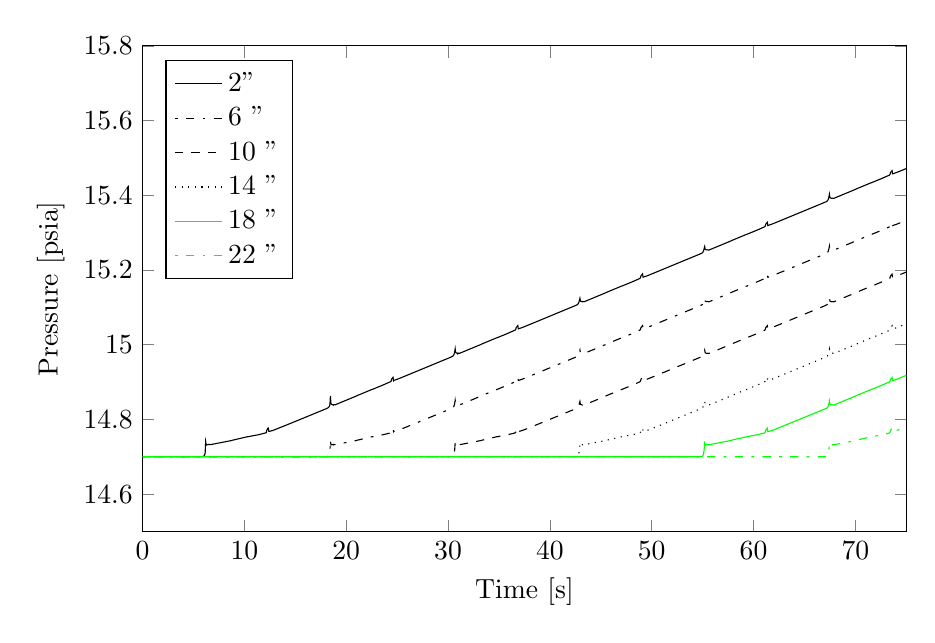
\begin{tikzpicture}

\begin{axis}[%
width=0.8\textwidth,
height=0.508815326102268\textwidth,
scale only axis,
xmin=0.0,
xmax=75.0,
xlabel={Time [s]},
ymin=14.5,
ymax=15.8,
ylabel={Pressure [psia]},
legend style={at={(0.03,0.97)},anchor=north west,draw=black,fill=white,legend cell align=left}
]
\addplot [
color=black,
solid
]
table[row sep=crcr]{
0 14.7007818222046\\
0.000862877757754177 14.7007904052734\\
0.0481183268129826 14.7007827758789\\
0.0981183275580406 14.7007827758789\\
0.148118332028389 14.7007827758789\\
0.198118329048157 14.7007827758789\\
0.248118326067925 14.7007827758789\\
0.298118323087692 14.7007827758789\\
0.348118335008621 14.7007827758789\\
0.398118317127228 14.7007827758789\\
0.448118329048157 14.7007827758789\\
0.498118340969086 14.7007827758789\\
0.548118352890015 14.7007837295532\\
0.598118305206299 14.7007837295532\\
0.648118317127228 14.7007837295532\\
0.698118329048157 14.7007837295532\\
0.748118340969086 14.7007837295532\\
0.798118352890015 14.7007837295532\\
0.848118305206299 14.7007837295532\\
0.898118317127228 14.7007837295532\\
0.948118329048157 14.7007837295532\\
0.998118340969086 14.7007837295532\\
1.04811835289001 14.7007827758789\\
1.0981183052063 14.7007827758789\\
1.14811837673187 14.7007827758789\\
1.19811832904816 14.7007827758789\\
1.24811828136444 14.7007827758789\\
1.29811835289001 14.7007827758789\\
1.3481183052063 14.7007827758789\\
1.39811837673187 14.7007827758789\\
1.44811832904816 14.7007827758789\\
1.49811828136444 14.7007827758789\\
1.54811835289001 14.7007827758789\\
1.5981183052063 14.7007827758789\\
1.64811837673187 14.7007827758789\\
1.69811832904816 14.7007827758789\\
1.74811828136444 14.7007827758789\\
1.79811835289001 14.7007827758789\\
1.8481183052063 14.7007827758789\\
1.89811837673187 14.7007827758789\\
1.94811832904816 14.7007827758789\\
1.99811828136444 14.7007827758789\\
2.04811835289001 14.7007827758789\\
2.0981183052063 14.7007827758789\\
2.14811825752258 14.7007827758789\\
2.19811820983887 14.7007827758789\\
2.24811840057373 14.7007827758789\\
2.29811835289001 14.7007827758789\\
2.3481183052063 14.7007827758789\\
2.39811825752258 14.7007827758789\\
2.44811820983887 14.7007827758789\\
2.49811840057373 14.7007827758789\\
2.54811835289001 14.7007827758789\\
2.5981183052063 14.7007827758789\\
2.64811825752258 14.7007827758789\\
2.69811820983887 14.7007827758789\\
2.74811840057373 14.7007827758789\\
2.79811835289001 14.7007827758789\\
2.8481183052063 14.7007827758789\\
2.89811825752258 14.7007827758789\\
2.94811820983887 14.7007827758789\\
2.99811840057373 14.7007827758789\\
3.04811835289001 14.7007827758789\\
3.0981183052063 14.7007827758789\\
3.14811825752258 14.7007827758789\\
3.19811820983887 14.7007827758789\\
3.24811840057373 14.7007827758789\\
3.29811835289001 14.7007827758789\\
3.3481183052063 14.7007827758789\\
3.39811825752258 14.7007827758789\\
3.44811820983887 14.7007827758789\\
3.49811840057373 14.7007827758789\\
3.54811835289001 14.7007827758789\\
3.5981183052063 14.7007827758789\\
3.64811825752258 14.7007827758789\\
3.69811820983887 14.7007827758789\\
3.74811840057373 14.7007827758789\\
3.79811835289001 14.7007827758789\\
3.8481183052063 14.7007827758789\\
3.89811825752258 14.7007827758789\\
3.94811820983887 14.7007827758789\\
3.99811840057373 14.7007827758789\\
4.04811811447144 14.7007827758789\\
4.0981183052063 14.7007827758789\\
4.14811849594116 14.7007827758789\\
4.19811820983887 14.7007827758789\\
4.24811840057373 14.7007827758789\\
4.29811811447144 14.7007827758789\\
4.3481183052063 14.7007827758789\\
4.39811849594116 14.7007827758789\\
4.44811820983887 14.7007827758789\\
4.49811840057373 14.7007827758789\\
4.54811811447144 14.7007827758789\\
4.5981183052063 14.7007827758789\\
4.64811849594116 14.7007827758789\\
4.69811820983887 14.7007827758789\\
4.74811840057373 14.7007827758789\\
4.79811811447144 14.7007827758789\\
4.8481183052063 14.7007827758789\\
4.89811849594116 14.7007827758789\\
4.94811820983887 14.7007827758789\\
4.99811840057373 14.7007827758789\\
5.04811811447144 14.7007827758789\\
5.0981183052063 14.7007827758789\\
5.14811849594116 14.7007827758789\\
5.19811820983887 14.7007827758789\\
5.24811840057373 14.7007827758789\\
5.29811811447144 14.7007827758789\\
5.3481183052063 14.7007827758789\\
5.39811849594116 14.7007827758789\\
5.44811820983887 14.7007837295532\\
5.49811840057373 14.7007837295532\\
5.54811811447144 14.7007837295532\\
5.5981183052063 14.7007846832275\\
5.64811849594116 14.7007865905762\\
5.69811820983887 14.7007904052734\\
5.74811840057373 14.700798034668\\
5.79811811447144 14.7008142471313\\
5.8481183052063 14.700852394104\\
5.89811849594116 14.7009391784668\\
5.94811820983887 14.7011461257935\\
5.99811840057373 14.7016353607178\\
6.04811811447144 14.7027759552002\\
6.0981183052063 14.7053365707397\\
6.14811849594116 14.7106647491455\\
6.19811820983887 14.740795135498\\
6.24811840057373 14.7324552536011\\
6.29811811447144 14.7318572998047\\
6.3481183052063 14.7325630187988\\
6.39811849594116 14.7329273223877\\
6.44811820983887 14.7330942153931\\
6.49811840057373 14.7331285476685\\
6.54811811447144 14.7327871322632\\
6.5981183052063 14.7332782745361\\
6.64811849594116 14.7326955795288\\
6.69811820983887 14.7328605651855\\
6.74811840057373 14.7331304550171\\
6.79811811447144 14.7333955764771\\
6.8481183052063 14.733660697937\\
6.89811849594116 14.7339267730713\\
6.94811820983887 14.7341918945313\\
6.99811840057373 14.7344570159912\\
7.04811811447144 14.7347221374512\\
7.0981183052063 14.7349872589111\\
7.14811849594116 14.7352533340454\\
7.19811820983887 14.7355184555054\\
7.24811840057373 14.7357835769653\\
7.29811811447144 14.7360486984253\\
7.3481183052063 14.7363147735596\\
7.39811849594116 14.7365798950195\\
7.44811820983887 14.7368450164795\\
7.49811840057373 14.7371110916138\\
7.54811811447144 14.7373762130737\\
7.5981183052063 14.737642288208\\
7.64811849594116 14.737907409668\\
7.69811820983887 14.7381725311279\\
7.74811840057373 14.7384386062622\\
7.79811811447144 14.7387037277222\\
7.8481183052063 14.7389698028564\\
7.89811849594116 14.7392349243164\\
7.94811820983887 14.7395009994507\\
7.99811840057373 14.7397661209106\\
8.04811859130859 14.7400321960449\\
8.09811878204346 14.7402982711792\\
8.148118019104 14.7405633926392\\
8.19811820983887 14.7408294677734\\
8.24811840057373 14.7410955429077\\
8.29811859130859 14.741361618042\\
8.34811878204346 14.741626739502\\
8.398118019104 14.7418928146362\\
8.44811820983887 14.7421588897705\\
8.49811840057373 14.7424249649048\\
8.54811859130859 14.7426910400391\\
8.59811878204346 14.7429571151733\\
8.648118019104 14.7432231903076\\
8.69811820983887 14.7434892654419\\
8.74811840057373 14.7437553405762\\
8.79811859130859 14.7441720962524\\
8.84811878204346 14.7446508407593\\
8.898118019104 14.7449808120728\\
8.94811820983887 14.745304107666\\
8.99811840057373 14.7456274032593\\
9.04811859130859 14.7459497451782\\
9.09811878204346 14.7462720870972\\
9.148118019104 14.7465944290161\\
9.19811820983887 14.7469158172607\\
9.24811840057373 14.7472372055054\\
9.29811859130859 14.7475576400757\\
9.34811878204346 14.747878074646\\
9.398118019104 14.7481985092163\\
9.44811820983887 14.7485189437866\\
9.49811840057373 14.7488384246826\\
9.54811859130859 14.7491579055786\\
9.59811878204346 14.7494773864746\\
9.648118019104 14.7497968673706\\
9.69811820983887 14.7501153945923\\
9.74811840057373 14.7504348754883\\
9.79811859130859 14.75075340271\\
9.84811878204346 14.7510719299316\\
9.898118019104 14.7513904571533\\
9.94811820983887 14.751708984375\\
9.99811840057373 14.7520275115967\\
10.0481185913086 14.7523460388184\\
10.0981187820435 14.75266456604\\
10.148118019104 14.7529821395874\\
10.1981182098389 14.7533006668091\\
10.2481184005737 14.7536106109619\\
10.2981185913086 14.7538509368896\\
10.3481187820435 14.7539186477661\\
10.398118019104 14.7541694641113\\
10.4481182098389 14.7544355392456\\
10.4981184005737 14.7547006607056\\
10.5481185913086 14.7549638748169\\
10.5981187820435 14.7552270889282\\
10.648118019104 14.7554883956909\\
10.6981182098389 14.7557487487793\\
10.7481184005737 14.7560081481934\\
10.7981185913086 14.7562665939331\\
10.8481187820435 14.7565231323242\\
10.898118019104 14.756778717041\\
10.9481182098389 14.7570323944092\\
10.9981184005737 14.757285118103\\
11.0481185913086 14.7575359344482\\
11.0981187820435 14.7577848434448\\
11.148118019104 14.7580318450928\\
11.1981182098389 14.7582759857178\\
11.2481184005737 14.7585182189941\\
11.2981185913086 14.7587585449219\\
11.3481187820435 14.7590141296387\\
11.398118019104 14.7593870162964\\
11.4481182098389 14.7596683502197\\
11.4981184005737 14.7599391937256\\
11.5481185913086 14.7602977752686\\
11.5981187820435 14.7607269287109\\
11.648118019104 14.7610492706299\\
11.6981182098389 14.7613697052002\\
11.7481184005737 14.7616968154907\\
11.7981185913086 14.7620315551758\\
11.8481187820435 14.762375831604\\
11.898118019104 14.7627325057983\\
11.9481182098389 14.7631044387817\\
11.9981184005737 14.7634944915771\\
12.0481185913086 14.7639093399048\\
12.0981187820435 14.7643556594849\\
12.148118019104 14.7648553848267\\
12.1981182098389 14.7710580825806\\
12.2481184005737 14.7730350494385\\
12.2981185913086 14.7768278121948\\
12.3481187820435 14.7772264480591\\
12.398118019104 14.7682046890259\\
12.4481182098389 14.7684726715088\\
12.4981184005737 14.7686452865601\\
12.5481185913086 14.7689199447632\\
12.5981187820435 14.7692365646362\\
12.648118019104 14.7695951461792\\
12.6981182098389 14.7699918746948\\
12.7481184005737 14.7704210281372\\
12.7981185913086 14.7708768844604\\
12.8481187820435 14.7713527679443\\
12.898118019104 14.7718439102173\\
12.9481182098389 14.772346496582\\
12.9981184005737 14.7728586196899\\
13.0481185913086 14.7733774185181\\
13.0981187820435 14.7739028930664\\
13.148118019104 14.7744369506836\\
13.1981182098389 14.7749700546265\\
13.2481184005737 14.7755060195923\\
13.2981185913086 14.7760457992554\\
13.3481187820435 14.7765893936157\\
13.398118019104 14.777135848999\\
13.4481182098389 14.777684211731\\
13.4981184005737 14.7782325744629\\
13.5481185913086 14.7787847518921\\
13.5981187820435 14.7793378829956\\
13.648118019104 14.7798919677734\\
13.6981182098389 14.780445098877\\
13.7481184005737 14.7809991836548\\
13.7981185913086 14.7815542221069\\
13.8481187820435 14.7821083068848\\
13.898118019104 14.7826623916626\\
13.9481182098389 14.7832164764404\\
13.9981184005737 14.7837715148926\\
14.0481185913086 14.7843255996704\\
14.0981187820435 14.7848806381226\\
14.148118019104 14.7854347229004\\
14.1981182098389 14.7859897613525\\
14.2481184005737 14.7865447998047\\
14.2981185913086 14.7870998382568\\
14.3481187820435 14.7876539230347\\
14.398118019104 14.7882089614868\\
14.4481182098389 14.788763999939\\
14.4981184005737 14.7893199920654\\
14.5481185913086 14.7898750305176\\
14.5981187820435 14.7904300689697\\
14.648118019104 14.7909851074219\\
14.6981182098389 14.7915410995483\\
14.7481184005737 14.7920961380005\\
14.7981185913086 14.792652130127\\
14.8481187820435 14.7932081222534\\
14.898118019104 14.7937641143799\\
14.9481182098389 14.7943201065063\\
14.9981184005737 14.7948760986328\\
15.0481185913086 14.7954320907593\\
15.0981187820435 14.7959880828857\\
15.148118019104 14.7965450286865\\
15.1981182098389 14.797101020813\\
15.2481184005737 14.7976579666138\\
15.2981185913086 14.7982139587402\\
15.3481187820435 14.7987699508667\\
15.398118019104 14.7993278503418\\
15.4481182098389 14.7998867034912\\
15.4981184005737 14.8004455566406\\
15.5481185913086 14.80100440979\\
15.5981187820435 14.8015642166138\\
15.648118019104 14.8021240234375\\
15.6981182098389 14.8026828765869\\
15.7481184005737 14.8032426834106\\
15.7981185913086 14.8038024902344\\
15.8481187820435 14.8043622970581\\
15.898118019104 14.8049211502075\\
15.9481182098389 14.8054809570313\\
15.9981184005737 14.806040763855\\
16.0481185913086 14.8066005706787\\
16.0981178283691 14.8071603775024\\
16.1481189727783 14.8077201843262\\
16.1981182098389 14.8082809448242\\
16.2481174468994 14.8088407516479\\
16.2981185913086 14.8094005584717\\
16.3481178283691 14.8099603652954\\
16.3981189727783 14.8105211257935\\
16.4481182098389 14.8110809326172\\
16.4981174468994 14.8116407394409\\
16.5481185913086 14.812201499939\\
16.5981178283691 14.8127613067627\\
16.6481189727783 14.8133220672607\\
16.6981182098389 14.8138818740845\\
16.7481174468994 14.8144426345825\\
16.7981185913086 14.8150033950806\\
16.8481178283691 14.8155641555786\\
16.8981189727783 14.8161239624023\\
16.9481182098389 14.8166847229004\\
16.9981174468994 14.8172454833984\\
17.0481185913086 14.8178062438965\\
17.0981178283691 14.8183670043945\\
17.1481189727783 14.8189277648926\\
17.1981182098389 14.8194885253906\\
17.2481174468994 14.8200492858887\\
17.2981185913086 14.8206100463867\\
17.3481178283691 14.8211708068848\\
17.3981189727783 14.8217325210571\\
17.4481182098389 14.8222932815552\\
17.4981174468994 14.8228540420532\\
17.5481185913086 14.8234148025513\\
17.5981178283691 14.8239765167236\\
17.6481189727783 14.8245372772217\\
17.6981182098389 14.825098991394\\
17.7481174468994 14.8256607055664\\
17.7981185913086 14.8262214660645\\
17.8481178283691 14.8267841339111\\
17.8981189727783 14.8273468017578\\
17.9481182098389 14.8279104232788\\
17.9981174468994 14.8284778594971\\
18.0481185913086 14.8290519714355\\
18.0981178283691 14.829644203186\\
18.1481189727783 14.8302764892578\\
18.1981182098389 14.8310070037842\\
18.2481174468994 14.8319625854492\\
18.2981185913086 14.8334188461304\\
18.3481178283691 14.8358945846558\\
18.3981189727783 14.8401155471802\\
18.4481182098389 14.8634014129639\\
18.4981174468994 14.8427610397339\\
18.5481185913086 14.8407258987427\\
18.5981178283691 14.8401498794556\\
18.6481189727783 14.8397159576416\\
18.6981182098389 14.8394355773926\\
18.7481174468994 14.8382635116577\\
18.7981185913086 14.8398170471191\\
18.8481178283691 14.8393144607544\\
18.8981189727783 14.8391933441162\\
18.9481182098389 14.8397607803345\\
18.9981174468994 14.8403234481812\\
19.0481185913086 14.8408851623535\\
19.0981178283691 14.8414478302002\\
19.1481189727783 14.8420104980469\\
19.1981182098389 14.8425731658936\\
19.2481174468994 14.8431358337402\\
19.2981185913086 14.8436985015869\\
19.3481178283691 14.8442611694336\\
19.3981189727783 14.8448238372803\\
19.4481182098389 14.845386505127\\
19.4981174468994 14.8459491729736\\
19.5481185913086 14.8465118408203\\
19.5981178283691 14.847074508667\\
19.6481189727783 14.8476371765137\\
19.6981182098389 14.8481998443604\\
19.7481174468994 14.8487634658813\\
19.7981185913086 14.849326133728\\
19.8481178283691 14.8498888015747\\
19.8981189727783 14.8504524230957\\
19.9481182098389 14.8510150909424\\
19.9981174468994 14.8515787124634\\
20.0481185913086 14.8521413803101\\
20.0981178283691 14.8527050018311\\
20.1481189727783 14.8532676696777\\
20.1981182098389 14.8538312911987\\
20.2481174468994 14.8543939590454\\
20.2981185913086 14.8549575805664\\
20.3481178283691 14.8555212020874\\
20.3981189727783 14.8560838699341\\
20.4481182098389 14.8566474914551\\
20.4981174468994 14.8572111129761\\
20.5481185913086 14.8577747344971\\
20.5981178283691 14.8583383560181\\
20.6481189727783 14.8589019775391\\
20.6981182098389 14.8594655990601\\
20.7481174468994 14.8600282669067\\
20.7981185913086 14.8605918884277\\
20.8481178283691 14.861156463623\\
20.8981189727783 14.861720085144\\
20.9481182098389 14.862283706665\\
20.9981174468994 14.862847328186\\
21.0481185913086 14.8635883331299\\
21.0981178283691 14.8642778396606\\
21.1481189727783 14.8648443222046\\
21.1981182098389 14.8654079437256\\
21.2481174468994 14.8659715652466\\
21.2981185913086 14.8665361404419\\
21.3481178283691 14.8670997619629\\
21.3981189727783 14.8676643371582\\
21.4481182098389 14.8682289123535\\
21.4981174468994 14.8687934875488\\
21.5481185913086 14.8693580627441\\
21.5981178283691 14.8699226379395\\
21.6481189727783 14.8704872131348\\
21.6981182098389 14.8710517883301\\
21.7481174468994 14.8716173171997\\
21.7981185913086 14.872181892395\\
21.8481178283691 14.8727474212646\\
21.8981189727783 14.87331199646\\
21.9481182098389 14.8738775253296\\
21.9981174468994 14.8744430541992\\
22.0481185913086 14.8750085830688\\
22.0981178283691 14.8755750656128\\
22.1481189727783 14.8761405944824\\
22.1981182098389 14.8767070770264\\
22.2481174468994 14.877272605896\\
22.2981185913086 14.8778390884399\\
22.3481178283691 14.8784055709839\\
22.3981189727783 14.8789720535278\\
22.4481182098389 14.8795394897461\\
22.4981174468994 14.8801002502441\\
22.5481185913086 14.8806104660034\\
22.5981178283691 14.8809413909912\\
22.6481189727783 14.8814888000488\\
22.6981182098389 14.8820505142212\\
22.7481174468994 14.8826103210449\\
22.7981185913086 14.8831701278687\\
22.8481178283691 14.8837299346924\\
22.8981189727783 14.8842887878418\\
22.9481182098389 14.8848485946655\\
22.9981174468994 14.8854074478149\\
23.0481185913086 14.8859663009644\\
23.0981178283691 14.8865251541138\\
23.1481189727783 14.8870830535889\\
23.1981182098389 14.887640953064\\
23.2481174468994 14.8881988525391\\
23.2981185913086 14.8887557983398\\
23.3481178283691 14.8893136978149\\
23.3981189727783 14.8898696899414\\
23.4481182098389 14.8904256820679\\
23.4981174468994 14.8909816741943\\
23.5481185913086 14.8915367126465\\
23.5981178283691 14.892107963562\\
23.6481189727783 14.8927640914917\\
23.6981182098389 14.8933391571045\\
23.7481174468994 14.8939056396484\\
23.7981185913086 14.8945360183716\\
23.8481178283691 14.8952054977417\\
23.8981189727783 14.8957862854004\\
23.9481182098389 14.8963661193848\\
23.9981174468994 14.8969507217407\\
24.0481185913086 14.8975391387939\\
24.0981178283691 14.8981342315674\\
24.1481189727783 14.8987369537354\\
24.1981182098389 14.8993482589722\\
24.2481174468994 14.8999719619751\\
24.2981185913086 14.9006118774414\\
24.3481178283691 14.9012727737427\\
24.3981189727783 14.9019622802734\\
24.4481182098389 14.9080896377563\\
24.4981174468994 14.9095897674561\\
24.5481185913086 14.9110231399536\\
24.5981178283691 14.9127502441406\\
24.6481189727783 14.9035682678223\\
24.6981182098389 14.9049625396729\\
24.7481174468994 14.9053144454956\\
24.7981185913086 14.9057331085205\\
24.8481178283691 14.9061670303345\\
24.8981189727783 14.906623840332\\
24.9481182098389 14.9071035385132\\
24.9981174468994 14.907603263855\\
25.0481185913086 14.9081182479858\\
25.0981178283691 14.9086456298828\\
25.1481189727783 14.9091806411743\\
25.1981182098389 14.909722328186\\
25.2481174468994 14.910267829895\\
25.2981185913086 14.9108171463013\\
25.3481178283691 14.9113683700562\\
25.3981189727783 14.911922454834\\
25.4481182098389 14.9124774932861\\
25.4981174468994 14.9130363464355\\
25.5481185913086 14.9135913848877\\
25.5981178283691 14.9141473770142\\
25.6481189727783 14.9147043228149\\
25.6981182098389 14.9152631759644\\
25.7481174468994 14.9158220291138\\
25.7981185913086 14.9163827896118\\
25.8481178283691 14.9169435501099\\
25.8981189727783 14.9175033569336\\
25.9481182098389 14.9180660247803\\
25.9981174468994 14.9186296463013\\
26.0481185913086 14.9191932678223\\
26.0981178283691 14.9197568893433\\
26.1481189727783 14.9203214645386\\
26.1981182098389 14.9208850860596\\
26.2481174468994 14.9214487075806\\
26.2981185913086 14.9220132827759\\
26.3481178283691 14.9225769042969\\
26.3981189727783 14.9231405258179\\
26.4481182098389 14.9237051010132\\
26.4981174468994 14.9242687225342\\
26.5481185913086 14.9248332977295\\
26.5981178283691 14.9253969192505\\
26.6481189727783 14.9259605407715\\
26.6981182098389 14.9265251159668\\
26.7481174468994 14.9270887374878\\
26.7981185913086 14.9276523590088\\
26.8481178283691 14.9282169342041\\
26.8981189727783 14.9287805557251\\
26.9481182098389 14.9293441772461\\
26.9981174468994 14.9299087524414\\
27.0481185913086 14.9304723739624\\
27.0981178283691 14.9310359954834\\
27.1481189727783 14.9316005706787\\
27.1981182098389 14.9321641921997\\
27.2481174468994 14.9327278137207\\
27.2981185913086 14.9332914352417\\
27.3481178283691 14.933856010437\\
27.3981189727783 14.934419631958\\
27.4481182098389 14.934983253479\\
27.4981174468994 14.9355478286743\\
27.5481185913086 14.9361114501953\\
27.5981178283691 14.9366750717163\\
27.6481189727783 14.9372396469116\\
27.6981182098389 14.9378032684326\\
27.7481174468994 14.9383668899536\\
27.7981185913086 14.9389314651489\\
27.8481178283691 14.9394950866699\\
27.8981189727783 14.9400587081909\\
27.9481182098389 14.9406223297119\\
27.9981174468994 14.9411869049072\\
28.0481185913086 14.9417505264282\\
28.0981178283691 14.9423141479492\\
28.1481189727783 14.9428787231445\\
28.1981182098389 14.9434366226196\\
28.2481174468994 14.9439992904663\\
28.2981185913086 14.9445629119873\\
28.3481178283691 14.9451265335083\\
28.3981189727783 14.9456901550293\\
28.4481182098389 14.9462547302246\\
28.4981174468994 14.9468183517456\\
28.5481185913086 14.9473819732666\\
28.5981178283691 14.9479465484619\\
28.6481189727783 14.9485101699829\\
28.6981182098389 14.9490747451782\\
28.7481174468994 14.9496383666992\\
28.7981185913086 14.9502019882202\\
28.8481178283691 14.9507665634155\\
28.8981189727783 14.9513301849365\\
28.9481182098389 14.9518947601318\\
28.9981174468994 14.9524583816528\\
29.0481185913086 14.9530220031738\\
29.0981178283691 14.9535865783691\\
29.1481189727783 14.9541501998901\\
29.1981182098389 14.9547147750854\\
29.2481174468994 14.9552783966064\\
29.2981185913086 14.9558420181274\\
29.3481178283691 14.9564065933228\\
29.3981189727783 14.9569702148438\\
29.4481182098389 14.9575347900391\\
29.4981174468994 14.9580984115601\\
29.5481185913086 14.9586620330811\\
29.5981178283691 14.9592266082764\\
29.6481189727783 14.9597902297974\\
29.6981182098389 14.9603548049927\\
29.7481174468994 14.9609184265137\\
29.7981185913086 14.9614820480347\\
29.8481178283691 14.96204662323\\
29.8981189727783 14.962610244751\\
29.9481182098389 14.9631748199463\\
29.9981174468994 14.9637393951416\\
30.0481185913086 14.9643039703369\\
30.0981178283691 14.9648685455322\\
30.1481189727783 14.9654340744019\\
30.1981182098389 14.9660015106201\\
30.2481174468994 14.96657371521\\
30.2981185913086 14.9671573638916\\
30.3481178283691 14.9677648544312\\
30.3981189727783 14.9684324264526\\
30.4481182098389 14.9692440032959\\
30.4981174468994 14.9703807830811\\
30.5481185913086 14.9722166061401\\
30.5981178283691 14.9753913879395\\
30.6481189727783 14.9805793762207\\
30.6981182098389 14.9893732070923\\
30.7481174468994 14.9791593551636\\
30.7981185913086 14.9783210754395\\
30.8481178283691 14.9778022766113\\
30.8981189727783 14.977442741394\\
30.9481182098389 14.9756059646606\\
30.9981174468994 14.9778232574463\\
31.0481185913086 14.9774351119995\\
31.0981178283691 14.9769945144653\\
31.1481189727783 14.9773254394531\\
31.1981182098389 14.9778985977173\\
31.2481174468994 14.9784622192383\\
31.2981185913086 14.9790258407593\\
31.3481178283691 14.9795904159546\\
31.3981189727783 14.9801540374756\\
31.4481182098389 14.9807186126709\\
31.4981174468994 14.9812822341919\\
31.5481185913086 14.9818468093872\\
31.5981178283691 14.9824113845825\\
31.6481189727783 14.9829750061035\\
31.6981182098389 14.9835395812988\\
31.7481174468994 14.9841041564941\\
31.7981185913086 14.9846677780151\\
31.8481178283691 14.9852323532104\\
31.8981189727783 14.9857969284058\\
31.9481182098389 14.9863605499268\\
31.9981174468994 14.9869251251221\\
32.0481185913086 14.9874897003174\\
32.0981178283691 14.9880542755127\\
32.1481170654297 14.9886178970337\\
32.1981201171875 14.989182472229\\
32.248119354248 14.9897470474243\\
32.2981185913086 14.9903116226196\\
32.3481178283691 14.9908752441406\\
32.3981170654297 14.9914398193359\\
32.4481201171875 14.9920043945313\\
32.498119354248 14.9925689697266\\
32.5481185913086 14.9931335449219\\
32.5981178283691 14.9936981201172\\
32.6481170654297 14.9942626953125\\
32.6981201171875 14.9948272705078\\
32.748119354248 14.9953918457031\\
32.7981185913086 14.9959564208984\\
32.8481178283691 14.9965209960938\\
32.8981170654297 14.9970855712891\\
32.9481201171875 14.9976501464844\\
32.998119354248 14.9982147216797\\
33.0481185913086 14.998779296875\\
33.0981178283691 14.9993438720703\\
33.1481170654297 14.9999084472656\\
33.1981201171875 15.0004730224609\\
33.248119354248 15.0010375976563\\
33.2981185913086 15.0018730163574\\
33.3481178283691 15.0024681091309\\
33.3981170654297 15.0030326843262\\
33.4481201171875 15.0035972595215\\
33.498119354248 15.0041627883911\\
33.5481185913086 15.0047273635864\\
33.5981178283691 15.0052928924561\\
33.6481170654297 15.0058574676514\\
33.6981201171875 15.006422996521\\
33.748119354248 15.0069885253906\\
33.7981185913086 15.0075531005859\\
33.8481178283691 15.0081186294556\\
33.8981170654297 15.0086841583252\\
33.9481201171875 15.0092496871948\\
33.998119354248 15.0098161697388\\
34.0481185913086 15.0103816986084\\
34.0981178283691 15.010947227478\\
34.1481170654297 15.011513710022\\
34.1981201171875 15.0120792388916\\
34.248119354248 15.0126457214355\\
34.2981185913086 15.0132122039795\\
34.3481178283691 15.0137777328491\\
34.3981170654297 15.0143442153931\\
34.4481201171875 15.0149116516113\\
34.498119354248 15.0154781341553\\
34.5481185913086 15.0160446166992\\
34.5981178283691 15.0166120529175\\
34.6481170654297 15.0171794891357\\
34.6981201171875 15.017746925354\\
34.748119354248 15.0182847976685\\
34.7981185913086 15.0187883377075\\
34.8481178283691 15.0191383361816\\
34.8981170654297 15.0197019577026\\
34.9481201171875 15.0202627182007\\
34.998119354248 15.0208234786987\\
35.0481185913086 15.0213832855225\\
35.0981178283691 15.0219440460205\\
35.1481170654297 15.0225038528442\\
35.1981201171875 15.023063659668\\
35.248119354248 15.0236234664917\\
35.2981185913086 15.0241832733154\\
35.3481178283691 15.0247421264648\\
35.3981170654297 15.0253009796143\\
35.4481201171875 15.0258598327637\\
35.498119354248 15.0264186859131\\
35.5481185913086 15.0269765853882\\
35.5981178283691 15.0275344848633\\
35.6481170654297 15.0280923843384\\
35.6981201171875 15.0286493301392\\
35.748119354248 15.0292062759399\\
35.7981185913086 15.0297622680664\\
35.8481178283691 15.030369758606\\
35.8981170654297 15.030987739563\\
35.9481201171875 15.0315570831299\\
35.998119354248 15.0321245193481\\
36.0481185913086 15.0327959060669\\
36.0981178283691 15.0334129333496\\
36.1481170654297 15.0339918136597\\
36.1981201171875 15.0345726013184\\
36.248119354248 15.0351572036743\\
36.2981185913086 15.0357475280762\\
36.3481178283691 15.0363435745239\\
36.3981170654297 15.0369482040405\\
36.4481201171875 15.037561416626\\
36.498119354248 15.0381889343262\\
36.5481185913086 15.0388317108154\\
36.5981178283691 15.0394983291626\\
36.6481170654297 15.0413951873779\\
36.6981201171875 15.0466623306274\\
36.748119354248 15.0479555130005\\
36.7981185913086 15.0494527816772\\
36.8481178283691 15.0512571334839\\
36.8981170654297 15.0426158905029\\
36.9481201171875 15.0431299209595\\
36.998119354248 15.0434913635254\\
37.0481185913086 15.0439138412476\\
37.0981178283691 15.0443544387817\\
37.1481170654297 15.0448169708252\\
37.1981201171875 15.0453023910522\\
37.248119354248 15.0458068847656\\
37.2981185913086 15.0463256835938\\
37.3481178283691 15.0468549728394\\
37.3981170654297 15.0473928451538\\
37.4481201171875 15.0479354858398\\
37.498119354248 15.0484819412231\\
37.5481185913086 15.0490322113037\\
37.5981178283691 15.0495843887329\\
37.6481170654297 15.0501384735107\\
37.6981201171875 15.0506935119629\\
37.748119354248 15.0512533187866\\
37.7981185913086 15.0518093109131\\
37.8481178283691 15.0523653030396\\
37.8981170654297 15.0529222488403\\
37.9481201171875 15.0534811019897\\
37.998119354248 15.0540409088135\\
38.0481185913086 15.0546016693115\\
38.0981178283691 15.0551624298096\\
38.1481170654297 15.0557241439819\\
38.1981201171875 15.0562858581543\\
38.248119354248 15.056848526001\\
38.2981185913086 15.057412147522\\
38.3481178283691 15.0579767227173\\
38.3981170654297 15.0585403442383\\
38.4481201171875 15.0591049194336\\
38.498119354248 15.0596685409546\\
38.5481185913086 15.0602321624756\\
38.5981178283691 15.0607967376709\\
38.6481170654297 15.0613613128662\\
38.6981201171875 15.0619249343872\\
38.748119354248 15.0624895095825\\
38.7981185913086 15.0630531311035\\
38.8481178283691 15.0636177062988\\
38.8981170654297 15.0641813278198\\
38.9481201171875 15.0647459030151\\
38.998119354248 15.0653095245361\\
39.0481185913086 15.0658740997314\\
39.0981178283691 15.0664377212524\\
39.1481170654297 15.0670022964478\\
39.1981201171875 15.0675659179688\\
39.248119354248 15.0681304931641\\
39.2981185913086 15.0686941146851\\
39.3481178283691 15.0692586898804\\
39.3981170654297 15.0698223114014\\
39.4481201171875 15.0703868865967\\
39.498119354248 15.0709505081177\\
39.5481185913086 15.0715141296387\\
39.5981178283691 15.072078704834\\
39.6481170654297 15.072642326355\\
39.6981201171875 15.0732069015503\\
39.748119354248 15.0737705230713\\
39.7981185913086 15.0743350982666\\
39.8481178283691 15.0748987197876\\
39.8981170654297 15.0754632949829\\
39.9481201171875 15.0760269165039\\
39.998119354248 15.0765914916992\\
40.0481185913086 15.0771551132202\\
40.0981178283691 15.0777196884155\\
40.1481170654297 15.0782833099365\\
40.1981201171875 15.0788469314575\\
40.248119354248 15.0794115066528\\
40.2981185913086 15.0799751281738\\
40.3481178283691 15.0805397033691\\
40.3981170654297 15.0811033248901\\
40.4481201171875 15.0816679000854\\
40.498119354248 15.0822315216064\\
40.5481185913086 15.0827960968018\\
40.5981178283691 15.0833597183228\\
40.6481170654297 15.0839233398438\\
40.6981201171875 15.0845289230347\\
40.748119354248 15.0850477218628\\
40.7981185913086 15.0856103897095\\
40.8481178283691 15.0861730575562\\
40.8981170654297 15.0867366790771\\
40.9481201171875 15.0873003005981\\
40.998119354248 15.0878648757935\\
41.0481185913086 15.0884284973145\\
41.0981178283691 15.0889930725098\\
41.1481170654297 15.0895566940308\\
41.1981201171875 15.0901212692261\\
41.248119354248 15.0906848907471\\
41.2981185913086 15.0912494659424\\
41.3481178283691 15.0918130874634\\
41.3981170654297 15.0923776626587\\
41.4481201171875 15.0929412841797\\
41.498119354248 15.093505859375\\
41.5481185913086 15.094069480896\\
41.5981178283691 15.0946340560913\\
41.6481170654297 15.0951976776123\\
41.6981201171875 15.0957622528076\\
41.748119354248 15.0963268280029\\
41.7981185913086 15.0968904495239\\
41.8481178283691 15.0974550247192\\
41.8981170654297 15.0980186462402\\
41.9481201171875 15.0985832214355\\
41.998119354248 15.0991468429565\\
42.0481185913086 15.0997114181519\\
42.0981178283691 15.1002750396729\\
42.1481170654297 15.1008396148682\\
42.1981201171875 15.1014041900635\\
42.248119354248 15.1019678115845\\
42.2981185913086 15.1025323867798\\
42.3481178283691 15.1030979156494\\
42.3981170654297 15.103663444519\\
42.4481201171875 15.1042318344116\\
42.498119354248 15.1048049926758\\
42.5481185913086 15.1053905487061\\
42.5981178283691 15.1060037612915\\
42.6481170654297 15.1066846847534\\
42.6981201171875 15.1075258255005\\
42.748119354248 15.1087274551392\\
42.7981185913086 15.1106977462769\\
42.8481178283691 15.1141042709351\\
42.8981170654297 15.1195669174194\\
42.9481201171875 15.1245193481445\\
42.998119354248 15.1171159744263\\
43.0481185913086 15.1164035797119\\
43.0981178283691 15.1159038543701\\
43.1481170654297 15.1155643463135\\
43.1981201171875 15.1150550842285\\
43.248119354248 15.1159658432007\\
43.2981185913086 15.1155271530151\\
43.3481178283691 15.1151285171509\\
43.3981170654297 15.1155605316162\\
43.4481201171875 15.1161308288574\\
43.498119354248 15.1166944503784\\
43.5481185913086 15.1172590255737\\
43.5981178283691 15.1178226470947\\
43.6481170654297 15.11838722229\\
43.6981201171875 15.118950843811\\
43.748119354248 15.1195154190063\\
43.7981185913086 15.1200799942017\\
43.8481178283691 15.120644569397\\
43.8981170654297 15.121208190918\\
43.9481201171875 15.1217727661133\\
43.998119354248 15.1223373413086\\
44.0481185913086 15.1229019165039\\
44.0981178283691 15.1234655380249\\
44.1481170654297 15.1240301132202\\
44.1981201171875 15.1245946884155\\
44.248119354248 15.1251592636108\\
44.2981185913086 15.1257238388062\\
44.3481178283691 15.1262884140015\\
44.3981170654297 15.1268520355225\\
44.4481201171875 15.1274166107178\\
44.498119354248 15.1279811859131\\
44.5481185913086 15.1285457611084\\
44.5981178283691 15.1291103363037\\
44.6481170654297 15.129674911499\\
44.6981201171875 15.1302394866943\\
44.748119354248 15.1308040618896\\
44.7981185913086 15.131368637085\\
44.8481178283691 15.1319332122803\\
44.8981170654297 15.1324977874756\\
44.9481201171875 15.1330623626709\\
44.998119354248 15.1336269378662\\
45.0481185913086 15.1341915130615\\
45.0981178283691 15.1347560882568\\
45.1481170654297 15.1353206634521\\
45.1981201171875 15.1358852386475\\
45.248119354248 15.1364498138428\\
45.2981185913086 15.1370143890381\\
45.3481178283691 15.1375799179077\\
45.3981170654297 15.138144493103\\
45.4481201171875 15.1387090682983\\
45.498119354248 15.139274597168\\
45.5481185913086 15.140118598938\\
45.5981178283691 15.1407032012939\\
45.6481170654297 15.1412677764893\\
45.6981201171875 15.1418323516846\\
45.748119354248 15.1423978805542\\
45.7981185913086 15.1429624557495\\
45.8481178283691 15.1435279846191\\
45.8981170654297 15.1440935134888\\
45.9481201171875 15.1446580886841\\
45.998119354248 15.1452236175537\\
46.0481185913086 15.1457891464233\\
46.0981178283691 15.146354675293\\
46.1481170654297 15.1469202041626\\
46.1981201171875 15.1474866867065\\
46.248119354248 15.1480522155762\\
46.2981185913086 15.1486177444458\\
46.3481178283691 15.1491842269897\\
46.3981170654297 15.1497497558594\\
46.4481201171875 15.1503162384033\\
46.498119354248 15.1508827209473\\
46.5481185913086 15.1514482498169\\
46.5981178283691 15.1520147323608\\
46.6481170654297 15.1525821685791\\
46.6981201171875 15.153148651123\\
46.748119354248 15.153715133667\\
46.7981185913086 15.1542825698853\\
46.8481178283691 15.1548500061035\\
46.8981170654297 15.1554174423218\\
46.9481201171875 15.15598487854\\
46.998119354248 15.1565198898315\\
47.0481185913086 15.1569948196411\\
47.0981178283691 15.157377243042\\
47.1481170654297 15.1579418182373\\
47.1981201171875 15.1585035324097\\
47.248119354248 15.1590642929077\\
47.2981185913086 15.1596250534058\\
47.3481178283691 15.1601848602295\\
47.3981170654297 15.1607456207275\\
47.4481201171875 15.1613054275513\\
47.498119354248 15.1618661880493\\
47.5481185913086 15.162425994873\\
47.5981178283691 15.1629848480225\\
47.6481170654297 15.1635446548462\\
47.6981201171875 15.1641035079956\\
47.748119354248 15.164662361145\\
47.7981185913086 15.1652212142944\\
47.8481178283691 15.1657800674438\\
47.8981170654297 15.1663379669189\\
47.9481201171875 15.166895866394\\
47.998119354248 15.1674528121948\\
48.0481185913086 15.1680097579956\\
48.0981178283691 15.1686220169067\\
48.1481170654297 15.1692304611206\\
48.1981201171875 15.1697988510132\\
48.248119354248 15.1703672409058\\
48.2981185913086 15.1710386276245\\
48.3481178283691 15.1716461181641\\
48.3981170654297 15.1722240447998\\
48.4481201171875 15.1728057861328\\
48.498119354248 15.1733903884888\\
48.5481185913086 15.1739807128906\\
48.5981178283691 15.1745777130127\\
48.6481170654297 15.175181388855\\
48.6981201171875 15.1757965087891\\
48.748119354248 15.1764230728149\\
48.7981185913086 15.1770677566528\\
48.8481178283691 15.1777353286743\\
48.8981170654297 15.1801261901855\\
48.9481201171875 15.1849517822266\\
48.998119354248 15.1862287521362\\
49.0481185913086 15.1877403259277\\
49.0981178283691 15.1895637512207\\
49.1481170654297 15.1808404922485\\
49.1981201171875 15.1813564300537\\
49.248119354248 15.1817207336426\\
49.2981185913086 15.1821441650391\\
49.3481178283691 15.1825857162476\\
49.3981170654297 15.183051109314\\
49.4481201171875 15.1835384368896\\
49.498119354248 15.1840438842773\\
49.5481185913086 15.1845626831055\\
49.5981178283691 15.1850929260254\\
49.6481170654297 15.1856307983398\\
49.6981201171875 15.1861743927002\\
49.748119354248 15.1867218017578\\
49.7981185913086 15.1872711181641\\
49.8481178283691 15.1878242492676\\
49.8981170654297 15.1883783340454\\
49.9481201171875 15.1889333724976\\
49.998119354248 15.1894941329956\\
50.0481185913086 15.1900491714478\\
50.0981178283691 15.1906051635742\\
50.1481170654297 15.1911630630493\\
50.1981201171875 15.1917219161987\\
50.248119354248 15.1922817230225\\
50.2981185913086 15.1928424835205\\
50.3481178283691 15.1934032440186\\
50.3981170654297 15.1939649581909\\
50.4481201171875 15.194525718689\\
50.498119354248 15.19508934021\\
50.5481185913086 15.195652961731\\
50.5981178283691 15.196216583252\\
50.6481170654297 15.1967811584473\\
50.6981201171875 15.1973447799683\\
50.748119354248 15.1979093551636\\
50.7981185913086 15.1984729766846\\
50.8481178283691 15.1990375518799\\
50.8981170654297 15.1996011734009\\
50.9481201171875 15.2001657485962\\
50.998119354248 15.2007303237915\\
51.0481185913086 15.2012939453125\\
51.0981178283691 15.2018585205078\\
51.1481170654297 15.2024221420288\\
51.1981201171875 15.2029867172241\\
51.248119354248 15.2035503387451\\
51.2981185913086 15.2041149139404\\
51.3481178283691 15.2046794891357\\
51.3981170654297 15.2052431106567\\
51.4481201171875 15.2058076858521\\
51.498119354248 15.206371307373\\
51.5481185913086 15.2069358825684\\
51.5981178283691 15.2074995040894\\
51.6481170654297 15.2080640792847\\
51.6981201171875 15.2086277008057\\
51.748119354248 15.209192276001\\
51.7981185913086 15.209755897522\\
51.8481178283691 15.2103204727173\\
51.8981170654297 15.2108840942383\\
51.9481201171875 15.2114486694336\\
51.998119354248 15.2120122909546\\
52.0481185913086 15.2125768661499\\
52.0981178283691 15.2131404876709\\
52.1481170654297 15.2137050628662\\
52.1981201171875 15.2142696380615\\
52.248119354248 15.2148332595825\\
52.2981185913086 15.2153978347778\\
52.3481178283691 15.2159614562988\\
52.3981170654297 15.2165260314941\\
52.4481201171875 15.2170896530151\\
52.498119354248 15.2176542282104\\
52.5481185913086 15.2182178497314\\
52.5981178283691 15.2187824249268\\
52.6481170654297 15.2193460464478\\
52.6981201171875 15.2199106216431\\
52.748119354248 15.2204742431641\\
52.7981185913086 15.2210388183594\\
52.8481178283691 15.2216024398804\\
52.8981170654297 15.2221660614014\\
52.9481201171875 15.2227306365967\\
52.998119354248 15.2232942581177\\
53.0481185913086 15.223858833313\\
53.0981178283691 15.224422454834\\
53.1481170654297 15.2249870300293\\
53.1981201171875 15.225549697876\\
53.248119354248 15.2261095046997\\
53.2981185913086 15.2266731262207\\
53.3481178283691 15.2272367477417\\
53.3981170654297 15.2278003692627\\
53.4481201171875 15.2283639907837\\
53.498119354248 15.228928565979\\
53.5481185913086 15.2294921875\\
53.5981178283691 15.2300567626953\\
53.6481170654297 15.2306213378906\\
53.6981201171875 15.2311849594116\\
53.748119354248 15.2317495346069\\
53.7981185913086 15.2323131561279\\
53.8481178283691 15.2328777313232\\
53.8981170654297 15.2334413528442\\
53.9481201171875 15.2340059280396\\
53.998119354248 15.2345695495605\\
54.0481185913086 15.2351341247559\\
54.0981178283691 15.2356986999512\\
54.1481170654297 15.2362623214722\\
54.1981201171875 15.2368268966675\\
54.248119354248 15.2373905181885\\
54.2981185913086 15.2379550933838\\
54.3481178283691 15.2385187149048\\
54.3981170654297 15.2390832901001\\
54.4481201171875 15.2396478652954\\
54.498119354248 15.2402124404907\\
54.5481185913086 15.240777015686\\
54.5981178283691 15.2413415908813\\
54.6481170654297 15.2419080734253\\
54.6981201171875 15.2424764633179\\
54.748119354248 15.243049621582\\
54.7981185913086 15.2436351776123\\
54.8481178283691 15.2442493438721\\
54.8981170654297 15.2449312210083\\
54.9481201171875 15.2457752227783\\
54.998119354248 15.2469844818115\\
55.0481185913086 15.248969078064\\
55.0981178283691 15.2524003982544\\
55.1481170654297 15.2578907012939\\
55.1981201171875 15.2626705169678\\
55.248119354248 15.2553386688232\\
55.2981185913086 15.2546329498291\\
55.3481178283691 15.2541351318359\\
55.3981170654297 15.2537984848022\\
55.4481201171875 15.25377368927\\
55.498119354248 15.2541856765747\\
55.5481185913086 15.2537565231323\\
55.5981178283691 15.2533655166626\\
55.6481170654297 15.2538061141968\\
55.6981201171875 15.254376411438\\
55.748119354248 15.254940032959\\
55.7981185913086 15.2555046081543\\
55.8481178283691 15.2560682296753\\
55.8981170654297 15.2566328048706\\
55.9481201171875 15.2571973800659\\
55.998119354248 15.2577610015869\\
56.0481185913086 15.2583255767822\\
56.0981178283691 15.2588901519775\\
56.1481170654297 15.2594537734985\\
56.1981201171875 15.2600183486938\\
56.248119354248 15.2605829238892\\
56.2981185913086 15.2611474990845\\
56.3481178283691 15.2617120742798\\
56.3981170654297 15.2622766494751\\
56.4481201171875 15.2628402709961\\
56.498119354248 15.2634048461914\\
56.5481185913086 15.2639694213867\\
56.5981178283691 15.264533996582\\
56.6481170654297 15.2650985717773\\
56.6981201171875 15.2656631469727\\
56.748119354248 15.266227722168\\
56.7981185913086 15.266791343689\\
56.8481178283691 15.2673559188843\\
56.8981170654297 15.2679204940796\\
56.9481201171875 15.2684850692749\\
56.998119354248 15.2690496444702\\
57.0481185913086 15.2696142196655\\
57.0981178283691 15.2701797485352\\
57.1481170654297 15.2707443237305\\
57.1981201171875 15.2713088989258\\
57.248119354248 15.2718734741211\\
57.2981185913086 15.2724380493164\\
57.3481178283691 15.2730026245117\\
57.3981170654297 15.273567199707\\
57.4481201171875 15.2741317749023\\
57.498119354248 15.274697303772\\
57.5481185913086 15.2752618789673\\
57.5981178283691 15.2758264541626\\
57.6481170654297 15.2763910293579\\
57.6981201171875 15.2769556045532\\
57.748119354248 15.2775220870972\\
57.7981185913086 15.2783651351929\\
57.8481178283691 15.2789487838745\\
57.8981170654297 15.2795133590698\\
57.9481201171875 15.2800788879395\\
57.998119354248 15.2806434631348\\
58.0481185913086 15.2812089920044\\
58.0981178283691 15.2817735671997\\
58.1481170654297 15.2823390960693\\
58.1981201171875 15.282904624939\\
58.248119354248 15.2834701538086\\
58.2981185913086 15.2840356826782\\
58.3481178283691 15.2846012115479\\
58.3981170654297 15.2851667404175\\
58.4481201171875 15.2857332229614\\
58.498119354248 15.2862987518311\\
58.5481185913086 15.2868642807007\\
58.5981178283691 15.2874307632446\\
58.6481170654297 15.2879962921143\\
58.6981201171875 15.2885627746582\\
58.748119354248 15.2891292572021\\
58.7981185913086 15.2896957397461\\
58.8481178283691 15.29026222229\\
58.8981170654297 15.290828704834\\
58.9481201171875 15.2913951873779\\
58.998119354248 15.2919626235962\\
59.0481185913086 15.2925291061401\\
59.0981178283691 15.2930965423584\\
59.1481170654297 15.2936639785767\\
59.1981201171875 15.2942314147949\\
59.248119354248 15.2947692871094\\
59.2981185913086 15.2952470779419\\
59.3481178283691 15.2956266403198\\
59.3981170654297 15.2961912155151\\
59.4481201171875 15.2967529296875\\
59.498119354248 15.2973136901855\\
59.5481185913086 15.2978744506836\\
59.5981178283691 15.2984352111816\\
59.6481170654297 15.2989959716797\\
59.6981201171875 15.2995557785034\\
59.748119354248 15.3001165390015\\
59.7981185913086 15.3006763458252\\
59.8481178283691 15.3012361526489\\
59.8981170654297 15.3017959594727\\
59.9481201171875 15.3023548126221\\
59.998119354248 15.3029136657715\\
60.0467147827148 15.3034572601318\\
60.0967140197754 15.3040161132813\\
60.1467132568359 15.3045740127563\\
60.1967124938965 15.3051328659058\\
60.246711730957 15.3056907653809\\
60.2967147827148 15.3062477111816\\
60.3467140197754 15.3068542480469\\
60.3967132568359 15.3074636459351\\
60.4467124938965 15.3080320358276\\
60.496711730957 15.3086004257202\\
60.5467147827148 15.3092632293701\\
60.5967140197754 15.3098726272583\\
60.6467132568359 15.310450553894\\
60.6967124938965 15.3110313415527\\
60.746711730957 15.311616897583\\
60.7967147827148 15.3122062683105\\
60.8467140197754 15.3128023147583\\
60.8967132568359 15.3134059906006\\
60.9467124938965 15.3140201568604\\
60.996711730957 15.3146467208862\\
61.0467147827148 15.3152894973755\\
61.0967140197754 15.3159551620483\\
61.1467132568359 15.3179874420166\\
61.1967124938965 15.3231363296509\\
61.246711730957 15.3244171142578\\
61.2967147827148 15.3259153366089\\
61.3467140197754 15.3277215957642\\
61.3967132568359 15.3190536499023\\
61.4467124938965 15.3195943832397\\
61.496711730957 15.3199577331543\\
61.5467147827148 15.3203802108765\\
61.5967140197754 15.320821762085\\
61.6467132568359 15.3212862014771\\
61.6967124938965 15.3217725753784\\
61.746711730957 15.3222770690918\\
61.7967147827148 15.3227968215942\\
61.8467140197754 15.3233261108398\\
61.8967132568359 15.3238639831543\\
61.9467124938965 15.3244066238403\\
61.996711730957 15.3249540328979\\
62.0467147827148 15.3255043029785\\
62.0967140197754 15.3260564804077\\
62.1467132568359 15.3266105651855\\
62.1967124938965 15.327166557312\\
62.246711730957 15.3277263641357\\
62.2967147827148 15.3282814025879\\
62.3467140197754 15.3288383483887\\
62.3967132568359 15.3293952941895\\
62.4467124938965 15.3299541473389\\
62.496711730957 15.3305139541626\\
62.5467147827148 15.3310747146606\\
62.5967140197754 15.3316354751587\\
62.6467132568359 15.3321971893311\\
62.6967124938965 15.3327589035034\\
62.746711730957 15.3333206176758\\
62.7967147827148 15.3338851928711\\
62.8467140197754 15.3344488143921\\
62.8967132568359 15.3350124359131\\
62.9467124938965 15.3355770111084\\
62.996711730957 15.3361406326294\\
63.0467147827148 15.3367071151733\\
63.0967140197754 15.33726978302\\
63.1467132568359 15.337833404541\\
63.1967124938965 15.3383979797363\\
63.246711730957 15.3389616012573\\
63.2967147827148 15.3395261764526\\
63.3467140197754 15.3400907516479\\
63.3967132568359 15.3406543731689\\
63.4467124938965 15.3412189483643\\
63.496711730957 15.3417825698853\\
63.5467147827148 15.3423471450806\\
63.5967140197754 15.3429107666016\\
63.6467132568359 15.3434753417969\\
63.6967124938965 15.3440399169922\\
63.746711730957 15.3446035385132\\
63.7967147827148 15.3451681137085\\
63.8467140197754 15.3457317352295\\
63.8967132568359 15.3462963104248\\
63.9467124938965 15.3468599319458\\
63.996711730957 15.3474245071411\\
64.0467147827148 15.3479881286621\\
64.0967102050781 15.3485527038574\\
64.1467132568359 15.3491172790527\\
64.1967163085938 15.3496809005737\\
64.246711730957 15.350245475769\\
64.2967147827148 15.35080909729\\
64.3467102050781 15.3513736724854\\
64.3967132568359 15.3519372940063\\
64.4467163085938 15.3525018692017\\
64.496711730957 15.3530654907227\\
64.5467147827148 15.353630065918\\
64.5967102050781 15.354193687439\\
64.6467132568359 15.3547582626343\\
64.6967163085938 15.3553218841553\\
64.746711730957 15.3558864593506\\
64.7967147827148 15.3564500808716\\
64.8467102050781 15.3570146560669\\
64.8967132568359 15.3575782775879\\
64.9467163085938 15.3581428527832\\
64.996711730957 15.3587064743042\\
65.0467147827148 15.3592710494995\\
65.0967102050781 15.3598346710205\\
65.1467132568359 15.3603992462158\\
65.1967163085938 15.3609628677368\\
65.246711730957 15.3615274429321\\
65.2967147827148 15.3620920181274\\
65.3467102050781 15.3626556396484\\
65.3967132568359 15.3632202148438\\
65.4467163085938 15.3637838363647\\
65.496711730957 15.3643484115601\\
65.5467147827148 15.3649120330811\\
65.5967102050781 15.3654794692993\\
65.6467132568359 15.3660354614258\\
65.6967163085938 15.3665981292725\\
65.746711730957 15.3671617507935\\
65.7967147827148 15.3677253723145\\
65.8467102050781 15.3682899475098\\
65.8967132568359 15.3688535690308\\
65.9467163085938 15.3694181442261\\
65.996711730957 15.3699817657471\\
66.0467147827148 15.3705463409424\\
66.0967102050781 15.3711099624634\\
66.1467132568359 15.3716745376587\\
66.1967163085938 15.372239112854\\
66.246711730957 15.372802734375\\
66.2967147827148 15.3733673095703\\
66.3467102050781 15.3739309310913\\
66.3967132568359 15.3744955062866\\
66.4467163085938 15.3750600814819\\
66.496711730957 15.3756237030029\\
66.5467147827148 15.3761882781982\\
66.5967102050781 15.3767518997192\\
66.6467132568359 15.3773164749146\\
66.6967163085938 15.3778810501099\\
66.746711730957 15.3784446716309\\
66.7967147827148 15.3790102005005\\
66.8467102050781 15.3795747756958\\
66.8967132568359 15.3801412582397\\
66.9467163085938 15.380708694458\\
66.996711730957 15.3812818527222\\
67.0467147827148 15.3818664550781\\
67.0967102050781 15.3824777603149\\
67.1467132568359 15.383152961731\\
67.1967163085938 15.3839807510376\\
67.246711730957 15.3851528167725\\
67.2967147827148 15.3870639801025\\
67.3467102050781 15.3903684616089\\
67.3967132568359 15.3957090377808\\
67.4467163085938 15.4029207229614\\
67.496711730957 15.3937177658081\\
67.5467147827148 15.3929452896118\\
67.5967102050781 15.3924388885498\\
67.6467132568359 15.3920907974243\\
67.6967163085938 15.3921298980713\\
67.746711730957 15.3924608230591\\
67.7967147827148 15.3920621871948\\
67.8467102050781 15.3916473388672\\
67.8967132568359 15.3920383453369\\
67.9467163085938 15.3926095962524\\
67.996711730957 15.3931741714478\\
68.0467147827148 15.3937377929688\\
68.0967102050781 15.3943023681641\\
68.1467132568359 15.3948669433594\\
68.1967163085938 15.3954305648804\\
68.246711730957 15.3959951400757\\
68.2967147827148 15.396559715271\\
68.3467102050781 15.3971242904663\\
68.3967132568359 15.3976879119873\\
68.4467163085938 15.3982524871826\\
68.496711730957 15.3988170623779\\
68.5467147827148 15.3993816375732\\
68.5967102050781 15.3999462127686\\
68.6467132568359 15.4005098342896\\
68.6967163085938 15.4010744094849\\
68.746711730957 15.4016389846802\\
68.7967147827148 15.4022035598755\\
68.8467102050781 15.4027681350708\\
68.8967132568359 15.4033327102661\\
68.9467163085938 15.4038972854614\\
68.996711730957 15.4044618606567\\
69.0467147827148 15.4050254821777\\
69.0967102050781 15.405590057373\\
69.1467132568359 15.4061546325684\\
69.1967163085938 15.4067192077637\\
69.246711730957 15.407283782959\\
69.2967147827148 15.4078483581543\\
69.3467102050781 15.4084138870239\\
69.3967132568359 15.4089784622192\\
69.4467163085938 15.4095430374146\\
69.496711730957 15.4101076126099\\
69.5467147827148 15.4106721878052\\
69.5967102050781 15.4112367630005\\
69.6467132568359 15.4118013381958\\
69.6967163085938 15.4123659133911\\
69.746711730957 15.4129314422607\\
69.7967147827148 15.4134960174561\\
69.8467102050781 15.4140605926514\\
69.8967132568359 15.4146251678467\\
69.9467163085938 15.4151906967163\\
69.996711730957 15.4157552719116\\
70.0467147827148 15.4165916442871\\
70.0967102050781 15.4171829223633\\
70.1467132568359 15.4177474975586\\
70.1967163085938 15.4183120727539\\
70.246711730957 15.4188776016235\\
70.2967147827148 15.4194421768188\\
70.3467102050781 15.4200077056885\\
70.3967132568359 15.4205732345581\\
70.4467163085938 15.4211387634277\\
70.496711730957 15.4217042922974\\
70.5467147827148 15.422269821167\\
70.5967102050781 15.4228353500366\\
70.6467132568359 15.4234008789063\\
70.6967163085938 15.4239664077759\\
70.746711730957 15.4245328903198\\
70.7967147827148 15.4250984191895\\
70.8467102050781 15.4256649017334\\
70.8967132568359 15.426230430603\\
70.9467163085938 15.426796913147\\
70.996711730957 15.4273633956909\\
71.0467147827148 15.4279298782349\\
71.0967102050781 15.4284963607788\\
71.1467132568359 15.4290628433228\\
71.1967163085938 15.4296293258667\\
71.246711730957 15.430196762085\\
71.2967147827148 15.4307632446289\\
71.3467102050781 15.4313306808472\\
71.3967132568359 15.4318981170654\\
71.4467163085938 15.4324655532837\\
71.496711730957 15.4330101013184\\
71.5467147827148 15.4335174560547\\
71.5967102050781 15.4338626861572\\
71.6467132568359 15.4344272613525\\
71.6967163085938 15.4349889755249\\
71.746711730957 15.4355497360229\\
71.7967147827148 15.436110496521\\
71.8467102050781 15.436671257019\\
71.8967132568359 15.4372320175171\\
71.9467163085938 15.4377927780151\\
71.996711730957 15.4383525848389\\
72.0467147827148 15.4389133453369\\
72.0967102050781 15.4394731521606\\
72.1467132568359 15.4400329589844\\
72.1967163085938 15.4405927658081\\
72.246711730957 15.4411516189575\\
72.2967147827148 15.4417104721069\\
72.3467102050781 15.4422693252563\\
72.3967132568359 15.4428281784058\\
72.4467163085938 15.4433870315552\\
72.496711730957 15.4439449310303\\
72.5467147827148 15.4445028305054\\
72.5967102050781 15.4451026916504\\
72.6467132568359 15.4457139968872\\
72.6967163085938 15.4462833404541\\
72.746711730957 15.4468517303467\\
72.7967147827148 15.4475049972534\\
72.8467102050781 15.4481182098389\\
72.8967132568359 15.4486970901489\\
72.9467163085938 15.4492769241333\\
72.996711730957 15.4498624801636\\
73.0467147827148 15.4504518508911\\
73.0967102050781 15.4510469436646\\
73.1467132568359 15.4516506195068\\
73.1967163085938 15.452262878418\\
73.246711730957 15.4528884887695\\
73.2967147827148 15.4535303115845\\
73.3467102050781 15.454195022583\\
73.3967132568359 15.4557666778564\\
73.4467163085938 15.4613199234009\\
73.496711730957 15.4626159667969\\
73.5467147827148 15.4640979766846\\
73.5967102050781 15.4658813476563\\
73.6467132568359 15.4573278427124\\
73.6967163085938 15.4578542709351\\
73.746711730957 15.4582147598267\\
73.7967147827148 15.4586372375488\\
73.8467102050781 15.459077835083\\
73.8967132568359 15.4595413208008\\
73.9467163085938 15.4600257873535\\
73.996711730957 15.4605302810669\\
74.0467147827148 15.461049079895\\
74.0967102050781 15.4615783691406\\
74.1467132568359 15.4621152877808\\
74.1967163085938 15.4626579284668\\
74.246711730957 15.4632043838501\\
74.2967147827148 15.4637546539307\\
74.3467102050781 15.4643068313599\\
74.3967132568359 15.4648609161377\\
74.4467163085938 15.4654169082642\\
74.496711730957 15.4659767150879\\
74.5467147827148 15.4665327072144\\
74.5967102050781 15.4670886993408\\
74.6467132568359 15.4676465988159\\
74.6967163085938 15.468204498291\\
74.746711730957 15.4687643051147\\
74.7967147827148 15.4693250656128\\
74.8467102050781 15.4698858261108\\
74.8967132568359 15.4704475402832\\
74.9467163085938 15.4710102081299\\
74.996711730957 15.4715709686279\\
};
\addlegendentry{2"};

\addplot [
color=black,
dash pattern=on 1pt off 3pt on 3pt off 3pt
]
table[row sep=crcr]{
0 14.7006950378418\\
0.000862877757754177 14.7007036209106\\
0.0481183268129826 14.7006950378418\\
0.0981183275580406 14.7006959915161\\
0.148118332028389 14.7006959915161\\
0.198118329048157 14.7006959915161\\
0.248118326067925 14.7006959915161\\
0.298118323087692 14.7006959915161\\
0.348118335008621 14.7006959915161\\
0.398118317127228 14.7006959915161\\
0.448118329048157 14.7006959915161\\
0.498118340969086 14.7006959915161\\
0.548118352890015 14.7006959915161\\
0.598118305206299 14.7006959915161\\
0.648118317127228 14.7006959915161\\
0.698118329048157 14.7006959915161\\
0.748118340969086 14.7006959915161\\
0.798118352890015 14.7006959915161\\
0.848118305206299 14.7006959915161\\
0.898118317127228 14.7006959915161\\
0.948118329048157 14.7006959915161\\
0.998118340969086 14.7006959915161\\
1.04811835289001 14.7006950378418\\
1.0981183052063 14.7006950378418\\
1.14811837673187 14.7006950378418\\
1.19811832904816 14.7006950378418\\
1.24811828136444 14.7006950378418\\
1.29811835289001 14.7006950378418\\
1.3481183052063 14.7006950378418\\
1.39811837673187 14.7006950378418\\
1.44811832904816 14.7006950378418\\
1.49811828136444 14.7006950378418\\
1.54811835289001 14.7006950378418\\
1.5981183052063 14.7006950378418\\
1.64811837673187 14.7006950378418\\
1.69811832904816 14.7006950378418\\
1.74811828136444 14.7006950378418\\
1.79811835289001 14.7006950378418\\
1.8481183052063 14.7006950378418\\
1.89811837673187 14.7006950378418\\
1.94811832904816 14.7006950378418\\
1.99811828136444 14.7006950378418\\
2.04811835289001 14.7006950378418\\
2.0981183052063 14.7006950378418\\
2.14811825752258 14.7006950378418\\
2.19811820983887 14.7006950378418\\
2.24811840057373 14.7006950378418\\
2.29811835289001 14.7006950378418\\
2.3481183052063 14.7006950378418\\
2.39811825752258 14.7006950378418\\
2.44811820983887 14.7006950378418\\
2.49811840057373 14.7006950378418\\
2.54811835289001 14.7006950378418\\
2.5981183052063 14.7006950378418\\
2.64811825752258 14.7006950378418\\
2.69811820983887 14.7006950378418\\
2.74811840057373 14.7006950378418\\
2.79811835289001 14.7006950378418\\
2.8481183052063 14.7006950378418\\
2.89811825752258 14.7006950378418\\
2.94811820983887 14.7006950378418\\
2.99811840057373 14.7006950378418\\
3.04811835289001 14.7006950378418\\
3.0981183052063 14.7006950378418\\
3.14811825752258 14.7006950378418\\
3.19811820983887 14.7006950378418\\
3.24811840057373 14.7006950378418\\
3.29811835289001 14.7006950378418\\
3.3481183052063 14.7006950378418\\
3.39811825752258 14.7006950378418\\
3.44811820983887 14.7006950378418\\
3.49811840057373 14.7006950378418\\
3.54811835289001 14.7006950378418\\
3.5981183052063 14.7006950378418\\
3.64811825752258 14.7006950378418\\
3.69811820983887 14.7006950378418\\
3.74811840057373 14.7006950378418\\
3.79811835289001 14.7006950378418\\
3.8481183052063 14.7006950378418\\
3.89811825752258 14.7006950378418\\
3.94811820983887 14.7006950378418\\
3.99811840057373 14.7006950378418\\
4.04811811447144 14.7006950378418\\
4.0981183052063 14.7006950378418\\
4.14811849594116 14.7006950378418\\
4.19811820983887 14.7006950378418\\
4.24811840057373 14.7006950378418\\
4.29811811447144 14.7006950378418\\
4.3481183052063 14.7006950378418\\
4.39811849594116 14.7006950378418\\
4.44811820983887 14.7006950378418\\
4.49811840057373 14.7006950378418\\
4.54811811447144 14.7006950378418\\
4.5981183052063 14.7006950378418\\
4.64811849594116 14.7006950378418\\
4.69811820983887 14.7006950378418\\
4.74811840057373 14.7006950378418\\
4.79811811447144 14.7006950378418\\
4.8481183052063 14.7006950378418\\
4.89811849594116 14.7006950378418\\
4.94811820983887 14.7006950378418\\
4.99811840057373 14.7006950378418\\
5.04811811447144 14.7006950378418\\
5.0981183052063 14.7006950378418\\
5.14811849594116 14.7006950378418\\
5.19811820983887 14.7006950378418\\
5.24811840057373 14.7006950378418\\
5.29811811447144 14.7006950378418\\
5.3481183052063 14.7006950378418\\
5.39811849594116 14.7006950378418\\
5.44811820983887 14.7006950378418\\
5.49811840057373 14.7006950378418\\
5.54811811447144 14.7006950378418\\
5.5981183052063 14.7006950378418\\
5.64811849594116 14.7006950378418\\
5.69811820983887 14.7006950378418\\
5.74811840057373 14.7006950378418\\
5.79811811447144 14.7006950378418\\
5.8481183052063 14.7006950378418\\
5.89811849594116 14.7006950378418\\
5.94811820983887 14.7006950378418\\
5.99811840057373 14.7006950378418\\
6.04811811447144 14.7006940841675\\
6.0981183052063 14.7006931304932\\
6.14811849594116 14.7006902694702\\
6.19811820983887 14.7006931304932\\
6.24811840057373 14.7006988525391\\
6.29811811447144 14.7006959915161\\
6.3481183052063 14.7006959915161\\
6.39811849594116 14.7006959915161\\
6.44811820983887 14.7006959915161\\
6.49811840057373 14.7006959915161\\
6.54811811447144 14.7006959915161\\
6.5981183052063 14.7006969451904\\
6.64811849594116 14.7006959915161\\
6.69811820983887 14.7006950378418\\
6.74811840057373 14.7006950378418\\
6.79811811447144 14.7006950378418\\
6.8481183052063 14.7006950378418\\
6.89811849594116 14.7006950378418\\
6.94811820983887 14.7006950378418\\
6.99811840057373 14.7006950378418\\
7.04811811447144 14.7006950378418\\
7.0981183052063 14.7006950378418\\
7.14811849594116 14.7006950378418\\
7.19811820983887 14.7006950378418\\
7.24811840057373 14.7006950378418\\
7.29811811447144 14.7006950378418\\
7.3481183052063 14.7006950378418\\
7.39811849594116 14.7006950378418\\
7.44811820983887 14.7006950378418\\
7.49811840057373 14.7006950378418\\
7.54811811447144 14.7006950378418\\
7.5981183052063 14.7006950378418\\
7.64811849594116 14.7006950378418\\
7.69811820983887 14.7006950378418\\
7.74811840057373 14.7006950378418\\
7.79811811447144 14.7006950378418\\
7.8481183052063 14.7006950378418\\
7.89811849594116 14.7006950378418\\
7.94811820983887 14.7006950378418\\
7.99811840057373 14.7006950378418\\
8.04811859130859 14.7006950378418\\
8.09811878204346 14.7006950378418\\
8.148118019104 14.7006950378418\\
8.19811820983887 14.7006950378418\\
8.24811840057373 14.7006950378418\\
8.29811859130859 14.7006950378418\\
8.34811878204346 14.7006950378418\\
8.398118019104 14.7006950378418\\
8.44811820983887 14.7006950378418\\
8.49811840057373 14.7006950378418\\
8.54811859130859 14.7006950378418\\
8.59811878204346 14.7006950378418\\
8.648118019104 14.7006950378418\\
8.69811820983887 14.7006950378418\\
8.74811840057373 14.7006950378418\\
8.79811859130859 14.7006950378418\\
8.84811878204346 14.7006950378418\\
8.898118019104 14.7006950378418\\
8.94811820983887 14.7006950378418\\
8.99811840057373 14.7006950378418\\
9.04811859130859 14.7006950378418\\
9.09811878204346 14.7006950378418\\
9.148118019104 14.7006950378418\\
9.19811820983887 14.7006950378418\\
9.24811840057373 14.7006950378418\\
9.29811859130859 14.7006950378418\\
9.34811878204346 14.7006950378418\\
9.398118019104 14.7006950378418\\
9.44811820983887 14.7006950378418\\
9.49811840057373 14.7006950378418\\
9.54811859130859 14.7006950378418\\
9.59811878204346 14.7006950378418\\
9.648118019104 14.7006950378418\\
9.69811820983887 14.7006950378418\\
9.74811840057373 14.7006950378418\\
9.79811859130859 14.7006950378418\\
9.84811878204346 14.7006950378418\\
9.898118019104 14.7006950378418\\
9.94811820983887 14.7006950378418\\
9.99811840057373 14.7006950378418\\
10.0481185913086 14.7006950378418\\
10.0981187820435 14.7006950378418\\
10.148118019104 14.7006950378418\\
10.1981182098389 14.7006950378418\\
10.2481184005737 14.7006950378418\\
10.2981185913086 14.7006950378418\\
10.3481187820435 14.7006950378418\\
10.398118019104 14.7006950378418\\
10.4481182098389 14.7006950378418\\
10.4981184005737 14.7006950378418\\
10.5481185913086 14.7006950378418\\
10.5981187820435 14.7006950378418\\
10.648118019104 14.7006950378418\\
10.6981182098389 14.7006950378418\\
10.7481184005737 14.7006950378418\\
10.7981185913086 14.7006950378418\\
10.8481187820435 14.7006950378418\\
10.898118019104 14.7006950378418\\
10.9481182098389 14.7006950378418\\
10.9981184005737 14.7006950378418\\
11.0481185913086 14.7006950378418\\
11.0981187820435 14.7006950378418\\
11.148118019104 14.7006950378418\\
11.1981182098389 14.7006950378418\\
11.2481184005737 14.7006950378418\\
11.2981185913086 14.7006950378418\\
11.3481187820435 14.7006950378418\\
11.398118019104 14.7006950378418\\
11.4481182098389 14.7006950378418\\
11.4981184005737 14.7006950378418\\
11.5481185913086 14.7006950378418\\
11.5981187820435 14.7006959915161\\
11.648118019104 14.7006959915161\\
11.6981182098389 14.7006950378418\\
11.7481184005737 14.7006950378418\\
11.7981185913086 14.7006950378418\\
11.8481187820435 14.7006950378418\\
11.898118019104 14.7006950378418\\
11.9481182098389 14.7006950378418\\
11.9981184005737 14.7006950378418\\
12.0481185913086 14.7006950378418\\
12.0981187820435 14.7006950378418\\
12.148118019104 14.7006950378418\\
12.1981182098389 14.7006950378418\\
12.2481184005737 14.7006950378418\\
12.2981185913086 14.7006950378418\\
12.3481187820435 14.7006940841675\\
12.398118019104 14.7006959915161\\
12.4481182098389 14.7006950378418\\
12.4981184005737 14.7006950378418\\
12.5481185913086 14.7006950378418\\
12.5981187820435 14.7006950378418\\
12.648118019104 14.7006950378418\\
12.6981182098389 14.7006950378418\\
12.7481184005737 14.7006959915161\\
12.7981185913086 14.7006959915161\\
12.8481187820435 14.7006959915161\\
12.898118019104 14.7006959915161\\
12.9481182098389 14.7006959915161\\
12.9981184005737 14.7006959915161\\
13.0481185913086 14.7006959915161\\
13.0981187820435 14.7006959915161\\
13.148118019104 14.7006959915161\\
13.1981182098389 14.7006959915161\\
13.2481184005737 14.7006959915161\\
13.2981185913086 14.7006959915161\\
13.3481187820435 14.7006959915161\\
13.398118019104 14.7006959915161\\
13.4481182098389 14.7006959915161\\
13.4981184005737 14.7006959915161\\
13.5481185913086 14.7006959915161\\
13.5981187820435 14.7006959915161\\
13.648118019104 14.7006959915161\\
13.6981182098389 14.7006959915161\\
13.7481184005737 14.7006959915161\\
13.7981185913086 14.7006959915161\\
13.8481187820435 14.7006959915161\\
13.898118019104 14.7006959915161\\
13.9481182098389 14.7006959915161\\
13.9981184005737 14.7006959915161\\
14.0481185913086 14.7006959915161\\
14.0981187820435 14.7006959915161\\
14.148118019104 14.7006959915161\\
14.1981182098389 14.7006959915161\\
14.2481184005737 14.7006959915161\\
14.2981185913086 14.7006959915161\\
14.3481187820435 14.7006959915161\\
14.398118019104 14.7006959915161\\
14.4481182098389 14.7006959915161\\
14.4981184005737 14.7006959915161\\
14.5481185913086 14.7006959915161\\
14.5981187820435 14.7006959915161\\
14.648118019104 14.7006959915161\\
14.6981182098389 14.7006959915161\\
14.7481184005737 14.7006959915161\\
14.7981185913086 14.7006959915161\\
14.8481187820435 14.7006959915161\\
14.898118019104 14.7006959915161\\
14.9481182098389 14.7006959915161\\
14.9981184005737 14.7006959915161\\
15.0481185913086 14.7006959915161\\
15.0981187820435 14.7006959915161\\
15.148118019104 14.7006959915161\\
15.1981182098389 14.7006959915161\\
15.2481184005737 14.7006959915161\\
15.2981185913086 14.7006959915161\\
15.3481187820435 14.7006959915161\\
15.398118019104 14.7006959915161\\
15.4481182098389 14.7006959915161\\
15.4981184005737 14.7006959915161\\
15.5481185913086 14.7006959915161\\
15.5981187820435 14.7006959915161\\
15.648118019104 14.7006959915161\\
15.6981182098389 14.7006959915161\\
15.7481184005737 14.7006959915161\\
15.7981185913086 14.7006959915161\\
15.8481187820435 14.7006959915161\\
15.898118019104 14.7006959915161\\
15.9481182098389 14.7006959915161\\
15.9981184005737 14.7006959915161\\
16.0481185913086 14.7006959915161\\
16.0981178283691 14.7006959915161\\
16.1481189727783 14.7006959915161\\
16.1981182098389 14.7006959915161\\
16.2481174468994 14.7006959915161\\
16.2981185913086 14.7006959915161\\
16.3481178283691 14.7006959915161\\
16.3981189727783 14.7006959915161\\
16.4481182098389 14.7006959915161\\
16.4981174468994 14.7006959915161\\
16.5481185913086 14.7006959915161\\
16.5981178283691 14.7006959915161\\
16.6481189727783 14.7006959915161\\
16.6981182098389 14.7006959915161\\
16.7481174468994 14.7006959915161\\
16.7981185913086 14.7006959915161\\
16.8481178283691 14.7006959915161\\
16.8981189727783 14.7006959915161\\
16.9481182098389 14.7006959915161\\
16.9981174468994 14.7006959915161\\
17.0481185913086 14.7006959915161\\
17.0981178283691 14.7006959915161\\
17.1481189727783 14.7006959915161\\
17.1981182098389 14.7006959915161\\
17.2481174468994 14.7006959915161\\
17.2981185913086 14.7006959915161\\
17.3481178283691 14.7006959915161\\
17.3981189727783 14.7006959915161\\
17.4481182098389 14.7006959915161\\
17.4981174468994 14.7006959915161\\
17.5481185913086 14.7006959915161\\
17.5981178283691 14.7006959915161\\
17.6481189727783 14.7006959915161\\
17.6981182098389 14.7006969451904\\
17.7481174468994 14.7006969451904\\
17.7981185913086 14.7006978988647\\
17.8481178283691 14.7006988525391\\
17.8981189727783 14.7007007598877\\
17.9481182098389 14.7007064819336\\
17.9981174468994 14.7007169723511\\
18.0481185913086 14.7007417678833\\
18.0981178283691 14.7007961273193\\
18.1481189727783 14.7009248733521\\
18.1981182098389 14.7012271881104\\
18.2481174468994 14.7019329071045\\
18.2981185913086 14.7035455703735\\
18.3481178283691 14.7070484161377\\
18.3981189727783 14.713942527771\\
18.4481182098389 14.7460117340088\\
18.4981174468994 14.7321634292603\\
18.5481185913086 14.732027053833\\
18.5981178283691 14.7326173782349\\
18.6481189727783 14.7329015731812\\
18.6981182098389 14.7330207824707\\
18.7481174468994 14.7319593429565\\
18.7981185913086 14.733546257019\\
18.8481178283691 14.7329893112183\\
18.8981189727783 14.7326202392578\\
18.9481182098389 14.732889175415\\
18.9981174468994 14.733154296875\\
19.0481185913086 14.7334184646606\\
19.0981178283691 14.7336835861206\\
19.1481189727783 14.7339487075806\\
19.1981182098389 14.7342128753662\\
19.2481174468994 14.7344779968262\\
19.2981185913086 14.7347431182861\\
19.3481178283691 14.7350082397461\\
19.3981189727783 14.7352724075317\\
19.4481182098389 14.7355375289917\\
19.4981174468994 14.7358026504517\\
19.5481185913086 14.7360677719116\\
19.5981178283691 14.7363328933716\\
19.6481189727783 14.7365980148315\\
19.6981182098389 14.7368631362915\\
19.7481174468994 14.7371282577515\\
19.7981185913086 14.7373933792114\\
19.8481178283691 14.7376594543457\\
19.8981189727783 14.7379245758057\\
19.9481182098389 14.7381896972656\\
19.9981174468994 14.7384557723999\\
20.0481185913086 14.7387208938599\\
20.0981178283691 14.7389860153198\\
20.1481189727783 14.7392520904541\\
20.1981182098389 14.7395172119141\\
20.2481174468994 14.7397832870483\\
20.2981185913086 14.7400493621826\\
20.3481178283691 14.7403154373169\\
20.3981189727783 14.7405815124512\\
20.4481182098389 14.7408475875854\\
20.4981174468994 14.7411136627197\\
20.5481185913086 14.741379737854\\
20.5981178283691 14.7416458129883\\
20.6481189727783 14.7419118881226\\
20.6981182098389 14.7421779632568\\
20.7481174468994 14.7424449920654\\
20.7981185913086 14.7427110671997\\
20.8481178283691 14.7429780960083\\
20.8981189727783 14.7432451248169\\
20.9481182098389 14.7435121536255\\
20.9981174468994 14.7437782287598\\
21.0481185913086 14.7442302703857\\
21.0981178283691 14.7446718215942\\
21.1481189727783 14.7449970245361\\
21.1981182098389 14.7453193664551\\
21.2481174468994 14.7456407546997\\
21.2981185913086 14.7459621429443\\
21.3481178283691 14.746283531189\\
21.3981189727783 14.7466049194336\\
21.4481182098389 14.7469253540039\\
21.4981174468994 14.7472457885742\\
21.5481185913086 14.7475662231445\\
21.5981178283691 14.7478866577148\\
21.6481189727783 14.7482061386108\\
21.6981182098389 14.7485256195068\\
21.7481174468994 14.7488451004028\\
21.7981185913086 14.7491645812988\\
21.8481178283691 14.7494831085205\\
21.8981189727783 14.7498025894165\\
21.9481182098389 14.7501211166382\\
21.9981174468994 14.7504405975342\\
22.0481185913086 14.7507591247559\\
22.0981178283691 14.7510776519775\\
22.1481189727783 14.7513961791992\\
22.1981182098389 14.7517147064209\\
22.2481174468994 14.7520341873169\\
22.2981185913086 14.7523527145386\\
22.3481178283691 14.7526712417603\\
22.3981189727783 14.7529907226563\\
22.4481182098389 14.7533092498779\\
22.4981174468994 14.7536220550537\\
22.5481185913086 14.7538795471191\\
22.5981178283691 14.7539396286011\\
22.6481189727783 14.7541971206665\\
22.6981182098389 14.7544660568237\\
22.7481174468994 14.754734992981\\
22.7981185913086 14.7550020217896\\
22.8481178283691 14.7552690505981\\
22.8981189727783 14.7555351257324\\
22.9481182098389 14.7558002471924\\
22.9981174468994 14.756064414978\\
23.0481185913086 14.7563276290894\\
23.0981178283691 14.7565898895264\\
23.1481189727783 14.7568511962891\\
23.1981182098389 14.7571115493774\\
23.2481174468994 14.7573699951172\\
23.2981185913086 14.7576284408569\\
23.3481178283691 14.757884979248\\
23.3981189727783 14.7581396102905\\
23.4481182098389 14.7583932876587\\
23.4981174468994 14.7586450576782\\
23.5481185913086 14.7588949203491\\
23.5981178283691 14.7591600418091\\
23.6481189727783 14.7595195770264\\
23.6981182098389 14.7598028182983\\
23.7481174468994 14.7600803375244\\
23.7981185913086 14.7604217529297\\
23.8481178283691 14.7608194351196\\
23.8981189727783 14.7611360549927\\
23.9481182098389 14.7614526748657\\
23.9981174468994 14.7617769241333\\
24.0481185913086 14.7621078491211\\
24.0981178283691 14.7624483108521\\
24.1481189727783 14.7628002166748\\
24.1981182098389 14.7631673812866\\
24.2481174468994 14.7635526657104\\
24.2981185913086 14.7639627456665\\
24.3481178283691 14.7644033432007\\
24.3981189727783 14.7648849487305\\
24.4481182098389 14.7711553573608\\
24.4981174468994 14.773042678833\\
24.5481185913086 14.7747421264648\\
24.5981178283691 14.7765598297119\\
24.6481189727783 14.7672233581543\\
24.6981182098389 14.7683687210083\\
24.7481174468994 14.7685441970825\\
24.7981185913086 14.7688217163086\\
24.8481178283691 14.7691411972046\\
24.8981189727783 14.7695026397705\\
24.9481182098389 14.7699022293091\\
24.9981174468994 14.7703332901001\\
25.0481185913086 14.7707901000977\\
25.0981178283691 14.7712669372559\\
25.1481189727783 14.7717590332031\\
25.1981182098389 14.7722616195679\\
25.2481174468994 14.7727746963501\\
25.2981185913086 14.7732934951782\\
25.3481178283691 14.7738189697266\\
25.3981189727783 14.7743492126465\\
25.4481182098389 14.7748832702637\\
25.4981174468994 14.7754240036011\\
25.5481185913086 14.7759628295898\\
25.5981178283691 14.7765054702759\\
25.6481189727783 14.7770500183105\\
25.6981182098389 14.7775983810425\\
25.7481174468994 14.7781476974487\\
25.7981185913086 14.7786998748779\\
25.8481178283691 14.7792530059814\\
25.8981189727783 14.7798051834106\\
25.9481182098389 14.7803602218628\\
25.9981174468994 14.7809171676636\\
26.0481185913086 14.78147315979\\
26.0981178283691 14.7820301055908\\
26.1481189727783 14.7825870513916\\
26.1981182098389 14.7831439971924\\
26.2481174468994 14.7837009429932\\
26.2981185913086 14.7842578887939\\
26.3481178283691 14.7848148345947\\
26.3981189727783 14.7853717803955\\
26.4481182098389 14.7859287261963\\
26.4981174468994 14.7864866256714\\
26.5481185913086 14.7870435714722\\
26.5981178283691 14.7876005172729\\
26.6481189727783 14.7881574630737\\
26.6981182098389 14.7887153625488\\
26.7481174468994 14.7892723083496\\
26.7981185913086 14.7898292541504\\
26.8481178283691 14.7903871536255\\
26.8981189727783 14.7909440994263\\
26.9481182098389 14.7915019989014\\
26.9981174468994 14.7920589447021\\
27.0481185913086 14.7926168441772\\
27.0981178283691 14.793173789978\\
27.1481189727783 14.7937316894531\\
27.1981182098389 14.7942886352539\\
27.2481174468994 14.794846534729\\
27.2981185913086 14.7954044342041\\
27.3481178283691 14.7959623336792\\
27.3981189727783 14.79651927948\\
27.4481182098389 14.7970771789551\\
27.4981174468994 14.7976350784302\\
27.5481185913086 14.7981929779053\\
27.5981178283691 14.7987508773804\\
27.6481189727783 14.7993087768555\\
27.6981182098389 14.7998666763306\\
27.7481174468994 14.8004245758057\\
27.7981185913086 14.8009824752808\\
27.8481178283691 14.8015413284302\\
27.8981189727783 14.8020992279053\\
27.9481182098389 14.8026571273804\\
27.9981174468994 14.8032150268555\\
28.0481185913086 14.8037738800049\\
28.0981178283691 14.80433177948\\
28.1481189727783 14.8048915863037\\
28.1981182098389 14.8054475784302\\
28.2481174468994 14.8060073852539\\
28.2981185913086 14.8065671920776\\
28.3481178283691 14.80712890625\\
28.3981189727783 14.807689666748\\
28.4481182098389 14.8082504272461\\
28.4981174468994 14.8088121414185\\
28.5481185913086 14.8093729019165\\
28.5981178283691 14.8099346160889\\
28.6481189727783 14.8104953765869\\
28.6981182098389 14.8110570907593\\
28.7481174468994 14.8116188049316\\
28.7981185913086 14.8121795654297\\
28.8481178283691 14.8127412796021\\
28.8981189727783 14.8133029937744\\
28.9481182098389 14.8138637542725\\
28.9981174468994 14.8144254684448\\
29.0481185913086 14.8149871826172\\
29.0981178283691 14.8155479431152\\
29.1481189727783 14.8161096572876\\
29.1981182098389 14.81667137146\\
29.2481174468994 14.8172330856323\\
29.2981185913086 14.8177947998047\\
29.3481178283691 14.8183555603027\\
29.3981189727783 14.8189172744751\\
29.4481182098389 14.8194789886475\\
29.4981174468994 14.8200407028198\\
29.5481185913086 14.8206024169922\\
29.5981178283691 14.8211641311646\\
29.6481189727783 14.8217258453369\\
29.6981182098389 14.8222875595093\\
29.7481174468994 14.8228492736816\\
29.7981185913086 14.823410987854\\
29.8481178283691 14.8239717483521\\
29.8981189727783 14.8245344161987\\
29.9481182098389 14.8250961303711\\
29.9981174468994 14.8256578445435\\
30.0481185913086 14.8262205123901\\
30.0981178283691 14.8267822265625\\
30.1481189727783 14.8273458480835\\
30.1981182098389 14.8279113769531\\
30.2481174468994 14.8284816741943\\
30.2981185913086 14.829062461853\\
30.3481178283691 14.8296680450439\\
30.3981189727783 14.8303337097168\\
30.4481182098389 14.8311433792114\\
30.4981174468994 14.8322772979736\\
30.5481185913086 14.8341112136841\\
30.5981178283691 14.8372840881348\\
30.6481189727783 14.8424692153931\\
30.6981182098389 14.8512620925903\\
30.7481174468994 14.841046333313\\
30.7981185913086 14.8402061462402\\
30.8481178283691 14.8396854400635\\
30.8981189727783 14.8393230438232\\
30.9481182098389 14.8374862670898\\
30.9981174468994 14.8397006988525\\
31.0481185913086 14.8393096923828\\
31.0981178283691 14.8388681411743\\
31.1481189727783 14.8391971588135\\
31.1981182098389 14.8397674560547\\
31.2481174468994 14.8403301239014\\
31.2981185913086 14.8408918380737\\
31.3481178283691 14.8414545059204\\
31.3981189727783 14.8420171737671\\
31.4481182098389 14.8425788879395\\
31.4981174468994 14.8431415557861\\
31.5481185913086 14.8437042236328\\
31.5981178283691 14.8442668914795\\
31.6481189727783 14.8448295593262\\
31.6981182098389 14.8453912734985\\
31.7481174468994 14.8459539413452\\
31.7981185913086 14.8465166091919\\
31.8481178283691 14.8470792770386\\
31.8981189727783 14.8476419448853\\
31.9481182098389 14.8482046127319\\
31.9981174468994 14.8487672805786\\
32.0481185913086 14.8493299484253\\
32.0981178283691 14.849892616272\\
32.1481170654297 14.8504552841187\\
32.1981201171875 14.8510189056396\\
32.248119354248 14.8515815734863\\
32.2981185913086 14.852144241333\\
32.3481178283691 14.8527069091797\\
32.3981170654297 14.8532695770264\\
32.4481201171875 14.853832244873\\
32.498119354248 14.8543949127197\\
32.5481185913086 14.8549575805664\\
32.5981178283691 14.8555212020874\\
32.6481170654297 14.8560838699341\\
32.6981201171875 14.8566465377808\\
32.748119354248 14.8572092056274\\
32.7981185913086 14.8577728271484\\
32.8481178283691 14.8583354949951\\
32.8981170654297 14.8588981628418\\
32.9481201171875 14.8594617843628\\
32.998119354248 14.8600244522095\\
33.0481185913086 14.8605871200562\\
33.0981178283691 14.8611507415771\\
33.1481170654297 14.8617134094238\\
33.1981201171875 14.8622760772705\\
33.248119354248 14.8628396987915\\
33.2981185913086 14.863673210144\\
33.3481178283691 14.8642673492432\\
33.3981170654297 14.8648300170898\\
33.4481201171875 14.8653936386108\\
33.498119354248 14.8659563064575\\
33.5481185913086 14.8665199279785\\
33.5981178283691 14.8670835494995\\
33.6481170654297 14.8676471710205\\
33.6981201171875 14.8682107925415\\
33.748119354248 14.8687744140625\\
33.7981185913086 14.8693380355835\\
33.8481178283691 14.8699016571045\\
33.8981170654297 14.8704662322998\\
33.9481201171875 14.8710298538208\\
33.998119354248 14.8715944290161\\
34.0481185913086 14.8721580505371\\
34.0981178283691 14.8727226257324\\
34.1481170654297 14.8732872009277\\
34.1981201171875 14.873851776123\\
34.248119354248 14.8744163513184\\
34.2981185913086 14.8749809265137\\
34.3481178283691 14.8755464553833\\
34.3981170654297 14.8761110305786\\
34.4481201171875 14.8766765594482\\
34.498119354248 14.8772420883179\\
34.5481185913086 14.8778066635132\\
34.5981178283691 14.8783731460571\\
34.6481170654297 14.8789386749268\\
34.6981201171875 14.8795042037964\\
34.748119354248 14.8800411224365\\
34.7981185913086 14.8805437088013\\
34.8481178283691 14.8808917999268\\
34.8981170654297 14.8814544677734\\
34.9481201171875 14.8820142745972\\
34.998119354248 14.8825731277466\\
35.0481185913086 14.8831329345703\\
35.0981178283691 14.8836917877197\\
35.1481170654297 14.8842506408691\\
35.1981201171875 14.8848094940186\\
35.248119354248 14.8853673934937\\
35.2981185913086 14.8859262466431\\
35.3481178283691 14.8864841461182\\
35.3981170654297 14.8870420455933\\
35.4481201171875 14.8875999450684\\
35.498119354248 14.8881568908691\\
35.5481185913086 14.8887138366699\\
35.5981178283691 14.8892707824707\\
35.6481170654297 14.8898267745972\\
35.6981201171875 14.8903837203979\\
35.748119354248 14.8909387588501\\
35.7981185913086 14.8914947509766\\
35.8481178283691 14.8921003341675\\
35.8981170654297 14.8927173614502\\
35.9481201171875 14.8932857513428\\
35.998119354248 14.8938522338867\\
36.0481185913086 14.8945226669312\\
36.0981178283691 14.8951387405396\\
36.1481170654297 14.8957166671753\\
36.1981201171875 14.8962965011597\\
36.248119354248 14.8968801498413\\
36.2981185913086 14.8974695205688\\
36.3481178283691 14.8980646133423\\
36.3981170654297 14.8986682891846\\
36.4481201171875 14.89928150177\\
36.498119354248 14.8999071121216\\
36.5481185913086 14.9005498886108\\
36.5981178283691 14.9012145996094\\
36.6481170654297 14.9031114578247\\
36.6981201171875 14.9083766937256\\
36.748119354248 14.9096698760986\\
36.7981185913086 14.9111661911011\\
36.8481178283691 14.9129705429077\\
36.8981170654297 14.9043283462524\\
36.9481201171875 14.9048414230347\\
36.998119354248 14.9052019119263\\
37.0481185913086 14.9056234359741\\
37.0981178283691 14.906063079834\\
37.1481170654297 14.9065256118774\\
37.1981201171875 14.9070100784302\\
37.248119354248 14.9075136184692\\
37.2981185913086 14.908031463623\\
37.3481178283691 14.9085597991943\\
37.3981170654297 14.9090967178345\\
37.4481201171875 14.9096384048462\\
37.498119354248 14.9101848602295\\
37.5481185913086 14.9107341766357\\
37.5981178283691 14.9112854003906\\
37.6481170654297 14.9118385314941\\
37.6981201171875 14.9123935699463\\
37.748119354248 14.9129524230957\\
37.7981185913086 14.9135074615479\\
37.8481178283691 14.9140625\\
37.8981170654297 14.9146194458008\\
37.9481201171875 14.9151773452759\\
37.998119354248 14.9157361984253\\
38.0481185913086 14.916296005249\\
38.0981178283691 14.9168567657471\\
38.1481170654297 14.9174175262451\\
38.1981201171875 14.9179782867432\\
38.248119354248 14.9185409545898\\
38.2981185913086 14.9191036224365\\
38.3481178283691 14.9196672439575\\
38.3981170654297 14.9202299118042\\
38.4481201171875 14.9207935333252\\
38.498119354248 14.9213571548462\\
38.5481185913086 14.9219207763672\\
38.5981178283691 14.9224843978882\\
38.6481170654297 14.9230470657349\\
38.6981201171875 14.9236106872559\\
38.748119354248 14.9241743087769\\
38.7981185913086 14.9247379302979\\
38.8481178283691 14.9253015518188\\
38.8981170654297 14.9258642196655\\
38.9481201171875 14.9264278411865\\
38.998119354248 14.9269914627075\\
39.0481185913086 14.9275550842285\\
39.0981178283691 14.9281187057495\\
39.1481170654297 14.9286823272705\\
39.1981201171875 14.9292449951172\\
39.248119354248 14.9298086166382\\
39.2981185913086 14.9303722381592\\
39.3481178283691 14.9309358596802\\
39.3981170654297 14.9314994812012\\
39.4481201171875 14.9320621490479\\
39.498119354248 14.9326257705688\\
39.5481185913086 14.9331893920898\\
39.5981178283691 14.9337530136108\\
39.6481170654297 14.9343166351318\\
39.6981201171875 14.9348793029785\\
39.748119354248 14.9354429244995\\
39.7981185913086 14.9360065460205\\
39.8481178283691 14.9365701675415\\
39.8981170654297 14.9371337890625\\
39.9481201171875 14.9376964569092\\
39.998119354248 14.9382600784302\\
40.0481185913086 14.9388236999512\\
40.0981178283691 14.9393873214722\\
40.1481170654297 14.9399509429932\\
40.1981201171875 14.9405145645142\\
40.248119354248 14.9410772323608\\
40.2981185913086 14.9416408538818\\
40.3481178283691 14.9422044754028\\
40.3981170654297 14.9427680969238\\
40.4481201171875 14.9433317184448\\
40.498119354248 14.9438943862915\\
40.5481185913086 14.9444580078125\\
40.5981178283691 14.9450216293335\\
40.6481170654297 14.9455852508545\\
40.6981201171875 14.9461898803711\\
40.748119354248 14.9467086791992\\
40.7981185913086 14.9472694396973\\
40.8481178283691 14.9478321075439\\
40.8981170654297 14.9483957290649\\
40.9481201171875 14.9489583969116\\
40.998119354248 14.9495220184326\\
41.0481185913086 14.9500856399536\\
41.0981178283691 14.9506492614746\\
41.1481170654297 14.9512128829956\\
41.1981201171875 14.9517765045166\\
41.248119354248 14.9523401260376\\
41.2981185913086 14.9529037475586\\
41.3481178283691 14.9534673690796\\
41.3981170654297 14.9540309906006\\
41.4481201171875 14.9545946121216\\
41.498119354248 14.9551572799683\\
41.5481185913086 14.9557209014893\\
41.5981178283691 14.9562845230103\\
41.6481170654297 14.9568481445313\\
41.6981201171875 14.9574117660522\\
41.748119354248 14.9579753875732\\
41.7981185913086 14.9585390090942\\
41.8481178283691 14.9591026306152\\
41.8981170654297 14.9596662521362\\
41.9481201171875 14.9602298736572\\
41.998119354248 14.9607934951782\\
42.0481185913086 14.9613571166992\\
42.0981178283691 14.9619207382202\\
42.1481170654297 14.9624843597412\\
42.1981201171875 14.9630479812622\\
42.248119354248 14.9636125564575\\
42.2981185913086 14.9641761779785\\
42.3481178283691 14.9647407531738\\
42.3981170654297 14.9653062820435\\
42.4481201171875 14.9658737182617\\
42.498119354248 14.9664468765259\\
42.5481185913086 14.9670314788818\\
42.5981178283691 14.9676446914673\\
42.6481170654297 14.9683246612549\\
42.6981201171875 14.9691648483276\\
42.748119354248 14.9703664779663\\
42.7981185913086 14.9723358154297\\
42.8481178283691 14.9757423400879\\
42.8981170654297 14.9812040328979\\
42.9481201171875 14.986156463623\\
42.998119354248 14.9787521362305\\
43.0481185913086 14.9780397415161\\
43.0981178283691 14.9775390625\\
43.1481170654297 14.9771995544434\\
43.1981201171875 14.9766893386841\\
43.248119354248 14.9776000976563\\
43.2981185913086 14.9771604537964\\
43.3481178283691 14.9767618179321\\
43.3981170654297 14.9771928787231\\
43.4481201171875 14.97776222229\\
43.498119354248 14.978325843811\\
43.5481185913086 14.978889465332\\
43.5981178283691 14.9794540405273\\
43.6481170654297 14.9800176620483\\
43.6981201171875 14.9805812835693\\
43.748119354248 14.9811449050903\\
43.7981185913086 14.9817085266113\\
43.8481178283691 14.9822731018066\\
43.8981170654297 14.9828367233276\\
43.9481201171875 14.9834003448486\\
43.998119354248 14.9839639663696\\
44.0481185913086 14.9845285415649\\
44.0981178283691 14.9850921630859\\
44.1481170654297 14.9856557846069\\
44.1981201171875 14.9862203598022\\
44.248119354248 14.9867839813232\\
44.2981185913086 14.9873476028442\\
44.3481178283691 14.9879121780396\\
44.3981170654297 14.9884757995605\\
44.4481201171875 14.9890403747559\\
44.498119354248 14.9896039962769\\
44.5481185913086 14.9901676177979\\
44.5981178283691 14.9907321929932\\
44.6481170654297 14.9912958145142\\
44.6981201171875 14.9918603897095\\
44.748119354248 14.9924240112305\\
44.7981185913086 14.9929885864258\\
44.8481178283691 14.9935522079468\\
44.8981170654297 14.9941167831421\\
44.9481201171875 14.9946804046631\\
44.998119354248 14.9952449798584\\
45.0481185913086 14.9958095550537\\
45.0981178283691 14.9963731765747\\
45.1481170654297 14.99693775177\\
45.1981201171875 14.9975023269653\\
45.248119354248 14.9980659484863\\
45.2981185913086 14.9986305236816\\
45.3481178283691 14.999195098877\\
45.3981170654297 14.9997596740723\\
45.4481201171875 15.0003232955933\\
45.498119354248 15.0008888244629\\
45.5481185913086 15.0017328262329\\
45.5981178283691 15.0023164749146\\
45.6481170654297 15.0028810501099\\
45.6981201171875 15.0034456253052\\
45.748119354248 15.0040102005005\\
45.7981185913086 15.0045747756958\\
45.8481178283691 15.0051393508911\\
45.8981170654297 15.0057039260864\\
45.9481201171875 15.0062694549561\\
45.998119354248 15.0068340301514\\
46.0481185913086 15.007399559021\\
46.0981178283691 15.0079641342163\\
46.1481170654297 15.0085296630859\\
46.1981201171875 15.0090951919556\\
46.248119354248 15.0096607208252\\
46.2981185913086 15.0102262496948\\
46.3481178283691 15.0107917785645\\
46.3981170654297 15.0113573074341\\
46.4481201171875 15.0119228363037\\
46.498119354248 15.0124883651733\\
46.5481185913086 15.0130548477173\\
46.5981178283691 15.0136213302612\\
46.6481170654297 15.0141868591309\\
46.6981201171875 15.0147533416748\\
46.748119354248 15.0153198242188\\
46.7981185913086 15.0158863067627\\
46.8481178283691 15.016453742981\\
46.8981170654297 15.0170202255249\\
46.9481201171875 15.0175876617432\\
46.998119354248 15.0181226730347\\
47.0481185913086 15.0185976028442\\
47.0981178283691 15.0189800262451\\
47.1481170654297 15.0195436477661\\
47.1981201171875 15.0201044082642\\
47.248119354248 15.0206651687622\\
47.2981185913086 15.0212249755859\\
47.3481178283691 15.021785736084\\
47.3981170654297 15.0223455429077\\
47.4481201171875 15.0229053497314\\
47.498119354248 15.0234651565552\\
47.5481185913086 15.0240240097046\\
47.5981178283691 15.0245838165283\\
47.6481170654297 15.0251426696777\\
47.6981201171875 15.0257015228271\\
47.748119354248 15.0262603759766\\
47.7981185913086 15.0268182754517\\
47.8481178283691 15.0273761749268\\
47.8981170654297 15.0279340744019\\
47.9481201171875 15.028491973877\\
47.998119354248 15.0290489196777\\
48.0481185913086 15.0296049118042\\
48.0981178283691 15.0302171707153\\
48.1481170654297 15.0308246612549\\
48.1981201171875 15.0313930511475\\
48.248119354248 15.03196144104\\
48.2981185913086 15.0326318740845\\
48.3481178283691 15.033239364624\\
48.3981170654297 15.0338172912598\\
48.4481201171875 15.0343980789185\\
48.498119354248 15.0349826812744\\
48.5481185913086 15.0355730056763\\
48.5981178283691 15.036169052124\\
48.6481170654297 15.0367736816406\\
48.6981201171875 15.0373868942261\\
48.748119354248 15.0380144119263\\
48.7981185913086 15.0386581420898\\
48.8481178283691 15.039324760437\\
48.8981170654297 15.0417156219482\\
48.9481201171875 15.0465412139893\\
48.998119354248 15.0478181838989\\
49.0481185913086 15.0493288040161\\
49.0981178283691 15.0511522293091\\
49.1481170654297 15.0424289703369\\
49.1981201171875 15.0429439544678\\
49.248119354248 15.0433082580566\\
49.2981185913086 15.0437316894531\\
49.3481178283691 15.0441732406616\\
49.3981170654297 15.0446376800537\\
49.4481201171875 15.0451240539551\\
49.498119354248 15.0456295013428\\
49.5481185913086 15.0461492538452\\
49.5981178283691 15.0466785430908\\
49.6481170654297 15.0472164154053\\
49.6981201171875 15.0477590560913\\
49.748119354248 15.0483055114746\\
49.7981185913086 15.0488557815552\\
49.8481178283691 15.0494079589844\\
49.8981170654297 15.0499620437622\\
49.9481201171875 15.0505170822144\\
49.998119354248 15.0510768890381\\
50.0481185913086 15.0516319274902\\
50.0981178283691 15.0521879196167\\
50.1481170654297 15.0527458190918\\
50.1981201171875 15.0533037185669\\
50.248119354248 15.0538635253906\\
50.2981185913086 15.0544233322144\\
50.3481178283691 15.0549850463867\\
50.3981170654297 15.0555458068848\\
50.4481201171875 15.0561065673828\\
50.498119354248 15.0566692352295\\
50.5481185913086 15.0572328567505\\
50.5981178283691 15.0577964782715\\
50.6481170654297 15.0583600997925\\
50.6981201171875 15.0589246749878\\
50.748119354248 15.0594882965088\\
50.7981185913086 15.0600519180298\\
50.8481178283691 15.0606155395508\\
50.8981170654297 15.0611801147461\\
50.9481201171875 15.0617437362671\\
50.998119354248 15.0623073577881\\
51.0481185913086 15.0628709793091\\
51.0981178283691 15.0634355545044\\
51.1481170654297 15.0639991760254\\
51.1981201171875 15.0645627975464\\
51.248119354248 15.0651273727417\\
51.2981185913086 15.0656909942627\\
51.3481178283691 15.0662546157837\\
51.3981170654297 15.0668182373047\\
51.4481201171875 15.0673828125\\
51.498119354248 15.067946434021\\
51.5481185913086 15.068510055542\\
51.5981178283691 15.0690746307373\\
51.6481170654297 15.0696382522583\\
51.6981201171875 15.0702018737793\\
51.748119354248 15.0707654953003\\
51.7981185913086 15.0713300704956\\
51.8481178283691 15.0718936920166\\
51.8981170654297 15.0724573135376\\
51.9481201171875 15.0730209350586\\
51.998119354248 15.0735855102539\\
52.0481185913086 15.0741491317749\\
52.0981178283691 15.0747127532959\\
52.1481170654297 15.0752763748169\\
52.1981201171875 15.0758409500122\\
52.248119354248 15.0764045715332\\
52.2981185913086 15.0769681930542\\
52.3481178283691 15.0775318145752\\
52.3981170654297 15.0780963897705\\
52.4481201171875 15.0786600112915\\
52.498119354248 15.0792236328125\\
52.5481185913086 15.0797872543335\\
52.5981178283691 15.0803518295288\\
52.6481170654297 15.0809154510498\\
52.6981201171875 15.0814790725708\\
52.748119354248 15.0820426940918\\
52.7981185913086 15.0826063156128\\
52.8481178283691 15.0831708908081\\
52.8981170654297 15.0837345123291\\
52.9481201171875 15.0842981338501\\
52.998119354248 15.0848617553711\\
53.0481185913086 15.0854263305664\\
53.0981178283691 15.0859899520874\\
53.1481170654297 15.0865535736084\\
53.1981201171875 15.0871162414551\\
53.248119354248 15.0876760482788\\
53.2981185913086 15.0882387161255\\
53.3481178283691 15.0888023376465\\
53.3981170654297 15.0893659591675\\
53.4481201171875 15.0899295806885\\
53.498119354248 15.0904932022095\\
53.5481185913086 15.0910577774048\\
53.5981178283691 15.0916213989258\\
53.6481170654297 15.0921850204468\\
53.6981201171875 15.0927495956421\\
53.748119354248 15.0933132171631\\
53.7981185913086 15.0938768386841\\
53.8481178283691 15.0944414138794\\
53.8981170654297 15.0950050354004\\
53.9481201171875 15.0955686569214\\
53.998119354248 15.0961332321167\\
54.0481185913086 15.0966968536377\\
54.0981178283691 15.0972604751587\\
54.1481170654297 15.097825050354\\
54.1981201171875 15.098388671875\\
54.248119354248 15.098952293396\\
54.2981185913086 15.0995168685913\\
54.3481178283691 15.1000804901123\\
54.3981170654297 15.1006450653076\\
54.4481201171875 15.1012086868286\\
54.498119354248 15.1017732620239\\
54.5481185913086 15.1023378372192\\
54.5981178283691 15.1029024124146\\
54.6481170654297 15.1034679412842\\
54.6981201171875 15.1040363311768\\
54.748119354248 15.1046094894409\\
54.7981185913086 15.1051950454712\\
54.8481178283691 15.105809211731\\
54.8981170654297 15.1064910888672\\
54.9481201171875 15.1073350906372\\
54.998119354248 15.1085433959961\\
55.0481185913086 15.1105279922485\\
55.0981178283691 15.113959312439\\
55.1481170654297 15.1194486618042\\
55.1981201171875 15.124228477478\\
55.248119354248 15.1168956756592\\
55.2981185913086 15.1161909103394\\
55.3481178283691 15.1156930923462\\
55.3981170654297 15.1153554916382\\
55.4481201171875 15.115330696106\\
55.498119354248 15.1157417297363\\
55.5481185913086 15.1153135299683\\
55.5981178283691 15.1149225234985\\
55.6481170654297 15.1153631210327\\
55.6981201171875 15.1159324645996\\
55.748119354248 15.1164960861206\\
55.7981185913086 15.1170597076416\\
55.8481178283691 15.1176242828369\\
55.8981170654297 15.1181879043579\\
55.9481201171875 15.1187524795532\\
55.998119354248 15.1193161010742\\
56.0481185913086 15.1198806762695\\
56.0981178283691 15.1204442977905\\
56.1481170654297 15.1210088729858\\
56.1981201171875 15.1215724945068\\
56.248119354248 15.1221370697021\\
56.2981185913086 15.1227016448975\\
56.3481178283691 15.1232652664185\\
56.3981170654297 15.1238298416138\\
56.4481201171875 15.1243934631348\\
56.498119354248 15.1249580383301\\
56.5481185913086 15.1255226135254\\
56.5981178283691 15.1260871887207\\
56.6481170654297 15.1266508102417\\
56.6981201171875 15.127215385437\\
56.748119354248 15.1277799606323\\
56.7981185913086 15.1283435821533\\
56.8481178283691 15.1289081573486\\
56.8981170654297 15.1294727325439\\
56.9481201171875 15.1300373077393\\
56.998119354248 15.1306009292603\\
57.0481185913086 15.1311655044556\\
57.0981178283691 15.1317300796509\\
57.1481170654297 15.1322946548462\\
57.1981201171875 15.1328592300415\\
57.248119354248 15.1334238052368\\
57.2981185913086 15.1339883804321\\
57.3481178283691 15.1345529556274\\
57.3981170654297 15.1351175308228\\
57.4481201171875 15.1356821060181\\
57.498119354248 15.1362466812134\\
57.5481185913086 15.1368112564087\\
57.5981178283691 15.137375831604\\
57.6481170654297 15.1379404067993\\
57.6981201171875 15.1385049819946\\
57.748119354248 15.1390705108643\\
57.7981185913086 15.13991355896\\
57.8481178283691 15.1404972076416\\
57.8981170654297 15.1410617828369\\
57.9481201171875 15.1416263580322\\
57.998119354248 15.1421918869019\\
58.0481185913086 15.1427564620972\\
58.0981178283691 15.1433219909668\\
58.1481170654297 15.1438865661621\\
58.1981201171875 15.1444520950317\\
58.248119354248 15.1450176239014\\
58.2981185913086 15.145583152771\\
58.3481178283691 15.1461477279663\\
58.3981170654297 15.1467132568359\\
58.4481201171875 15.1472787857056\\
58.498119354248 15.1478452682495\\
58.5481185913086 15.1484107971191\\
58.5981178283691 15.1489763259888\\
58.6481170654297 15.1495428085327\\
58.6981201171875 15.1501083374023\\
58.748119354248 15.1506748199463\\
58.7981185913086 15.1512413024902\\
58.8481178283691 15.1518077850342\\
58.8981170654297 15.1523742675781\\
58.9481201171875 15.1529407501221\\
58.998119354248 15.153507232666\\
59.0481185913086 15.1540746688843\\
59.0981178283691 15.1546411514282\\
59.1481170654297 15.1552085876465\\
59.1981201171875 15.1557760238647\\
59.248119354248 15.1563138961792\\
59.2981185913086 15.1567907333374\\
59.3481178283691 15.1571702957153\\
59.3981170654297 15.1577348709106\\
59.4481201171875 15.1582956314087\\
59.498119354248 15.1588563919067\\
59.5481185913086 15.1594171524048\\
59.5981178283691 15.1599779129028\\
59.6481170654297 15.1605386734009\\
59.6981201171875 15.1610984802246\\
59.748119354248 15.1616582870483\\
59.7981185913086 15.1622180938721\\
59.8481178283691 15.1627779006958\\
59.8981170654297 15.1633377075195\\
59.9481201171875 15.1638965606689\\
59.998119354248 15.1644563674927\\
60.0467147827148 15.1649990081787\\
60.0967140197754 15.1655578613281\\
60.1467132568359 15.1661157608032\\
60.1967124938965 15.1666736602783\\
60.246711730957 15.1672315597534\\
60.2967147827148 15.1677894592285\\
60.3467140197754 15.1683950424194\\
60.3967132568359 15.1690044403076\\
60.4467124938965 15.1695728302002\\
60.496711730957 15.1701412200928\\
60.5467147827148 15.1708030700684\\
60.5967140197754 15.1714124679565\\
60.6467132568359 15.1719903945923\\
60.6967124938965 15.172571182251\\
60.746711730957 15.1731567382813\\
60.7967147827148 15.1737461090088\\
60.8467140197754 15.1743421554565\\
60.8967132568359 15.1749458312988\\
60.9467124938965 15.1755590438843\\
60.996711730957 15.1761856079102\\
61.0467147827148 15.1768283843994\\
61.0967140197754 15.1774940490723\\
61.1467132568359 15.1795263290405\\
61.1967124938965 15.1846752166748\\
61.246711730957 15.1859560012817\\
61.2967147827148 15.1874542236328\\
61.3467140197754 15.1892604827881\\
61.3967132568359 15.180591583252\\
61.4467124938965 15.1811332702637\\
61.496711730957 15.1814956665039\\
61.5467147827148 15.1819181442261\\
61.5967140197754 15.1823596954346\\
61.6467132568359 15.1828241348267\\
61.6967124938965 15.1833095550537\\
61.746711730957 15.1838150024414\\
61.7967147827148 15.1843338012695\\
61.8467140197754 15.1848630905151\\
61.8967132568359 15.1854009628296\\
61.9467124938965 15.1859436035156\\
61.996711730957 15.1864910125732\\
62.0467147827148 15.1870403289795\\
62.0967140197754 15.1875925064087\\
62.1467132568359 15.1881465911865\\
62.1967124938965 15.188702583313\\
62.246711730957 15.1892623901367\\
62.2967147827148 15.1898174285889\\
62.3467140197754 15.1903743743896\\
62.3967132568359 15.1909313201904\\
62.4467124938965 15.1914901733398\\
62.496711730957 15.1920499801636\\
62.5467147827148 15.1926097869873\\
62.5967140197754 15.1931705474854\\
62.6467132568359 15.1937322616577\\
62.6967124938965 15.1942939758301\\
62.746711730957 15.1948556900024\\
62.7967147827148 15.1954193115234\\
62.8467140197754 15.1959829330444\\
62.8967132568359 15.1965475082397\\
62.9467124938965 15.1971111297607\\
62.996711730957 15.1976757049561\\
63.0467147827148 15.1982412338257\\
63.0967140197754 15.1988039016724\\
63.1467132568359 15.1993675231934\\
63.1967124938965 15.1999320983887\\
63.246711730957 15.2004957199097\\
63.2967147827148 15.201060295105\\
63.3467140197754 15.201623916626\\
63.3967132568359 15.2021884918213\\
63.4467124938965 15.2027521133423\\
63.496711730957 15.2033157348633\\
63.5467147827148 15.2038803100586\\
63.5967140197754 15.2044439315796\\
63.6467132568359 15.2050085067749\\
63.6967124938965 15.2055721282959\\
63.746711730957 15.2061367034912\\
63.7967147827148 15.2067003250122\\
63.8467140197754 15.2072649002075\\
63.8967132568359 15.2078285217285\\
63.9467124938965 15.2083930969238\\
63.996711730957 15.2089567184448\\
64.0467147827148 15.2095203399658\\
64.0967102050781 15.2100849151611\\
64.1467132568359 15.2106485366821\\
64.1967163085938 15.2112131118774\\
64.246711730957 15.2117767333984\\
64.2967147827148 15.2123413085938\\
64.3467102050781 15.2129049301147\\
64.3967132568359 15.2134685516357\\
64.4467163085938 15.2140331268311\\
64.496711730957 15.2145967483521\\
64.5467147827148 15.2151613235474\\
64.5967102050781 15.2157249450684\\
64.6467132568359 15.2162885665894\\
64.6967163085938 15.2168531417847\\
64.746711730957 15.2174167633057\\
64.7967147827148 15.217981338501\\
64.8467102050781 15.218544960022\\
64.8967132568359 15.2191095352173\\
64.9467163085938 15.2196731567383\\
64.996711730957 15.2202367782593\\
65.0467147827148 15.2208013534546\\
65.0967102050781 15.2213649749756\\
65.1467132568359 15.2219295501709\\
65.1967163085938 15.2224931716919\\
65.246711730957 15.2230567932129\\
65.2967147827148 15.2236213684082\\
65.3467102050781 15.2241849899292\\
65.3967132568359 15.2247495651245\\
65.4467163085938 15.2253131866455\\
65.496711730957 15.2258768081665\\
65.5467147827148 15.2264413833618\\
65.5967102050781 15.2270078659058\\
65.6467132568359 15.2275648117065\\
65.6967163085938 15.2281274795532\\
65.746711730957 15.2286911010742\\
65.7967147827148 15.2292547225952\\
65.8467102050781 15.2298183441162\\
65.8967132568359 15.2303819656372\\
65.9467163085938 15.2309465408325\\
65.996711730957 15.2315101623535\\
66.0467147827148 15.2320747375488\\
66.0967102050781 15.2326383590698\\
66.1467132568359 15.2332029342651\\
66.1967163085938 15.2337665557861\\
66.246711730957 15.2343311309814\\
66.2967147827148 15.2348947525024\\
66.3467102050781 15.2354593276978\\
66.3967132568359 15.2360229492188\\
66.4467163085938 15.2365875244141\\
66.496711730957 15.2371511459351\\
66.5467147827148 15.2377157211304\\
66.5967102050781 15.2382793426514\\
66.6467132568359 15.2388439178467\\
66.6967163085938 15.2394075393677\\
66.746711730957 15.239972114563\\
66.7967147827148 15.2405366897583\\
66.8467102050781 15.2411022186279\\
66.8967132568359 15.2416677474976\\
66.9467163085938 15.2422361373901\\
66.996711730957 15.24280834198\\
67.0467147827148 15.2433929443359\\
67.0967102050781 15.2440042495728\\
67.1467132568359 15.2446794509888\\
67.1967163085938 15.2455062866211\\
67.246711730957 15.2466793060303\\
67.2967147827148 15.2485904693604\\
67.3467102050781 15.2518939971924\\
67.3967132568359 15.2572345733643\\
67.4467163085938 15.2644462585449\\
67.496711730957 15.2552433013916\\
67.5467147827148 15.2544717788696\\
67.5967102050781 15.2539644241333\\
67.6467132568359 15.2536163330078\\
67.6967163085938 15.2536554336548\\
67.746711730957 15.2539863586426\\
67.7967147827148 15.2535877227783\\
67.8467102050781 15.2531728744507\\
67.8967132568359 15.2535638809204\\
67.9467163085938 15.2541351318359\\
67.996711730957 15.2546987533569\\
68.0467147827148 15.2552633285522\\
68.0967102050781 15.2558269500732\\
68.1467132568359 15.2563915252686\\
68.1967163085938 15.2569551467896\\
68.246711730957 15.2575197219849\\
68.2967147827148 15.2580842971802\\
68.3467102050781 15.2586479187012\\
68.3967132568359 15.2592124938965\\
68.4467163085938 15.2597770690918\\
68.496711730957 15.2603416442871\\
68.5467147827148 15.2609052658081\\
68.5967102050781 15.2614698410034\\
68.6467132568359 15.2620344161987\\
68.6967163085938 15.262598991394\\
68.746711730957 15.263162612915\\
68.7967147827148 15.2637271881104\\
68.8467102050781 15.2642917633057\\
68.8967132568359 15.264856338501\\
68.9467163085938 15.2654209136963\\
68.996711730957 15.2659854888916\\
69.0467147827148 15.2665491104126\\
69.0967102050781 15.2671136856079\\
69.1467132568359 15.2676782608032\\
69.1967163085938 15.2682428359985\\
69.246711730957 15.2688074111938\\
69.2967147827148 15.2693719863892\\
69.3467102050781 15.2699365615845\\
69.3967132568359 15.2705011367798\\
69.4467163085938 15.2710657119751\\
69.496711730957 15.2716302871704\\
69.5467147827148 15.2721948623657\\
69.5967102050781 15.272759437561\\
69.6467132568359 15.2733240127563\\
69.6967163085938 15.2738885879517\\
69.746711730957 15.2744541168213\\
69.7967147827148 15.2750186920166\\
69.8467102050781 15.2755832672119\\
69.8967132568359 15.2761478424072\\
69.9467163085938 15.2767124176025\\
69.996711730957 15.2772769927979\\
70.0467147827148 15.2781143188477\\
70.0967102050781 15.2787046432495\\
70.1467132568359 15.2792692184448\\
70.1967163085938 15.2798337936401\\
70.246711730957 15.2803993225098\\
70.2967147827148 15.2809638977051\\
70.3467102050781 15.2815294265747\\
70.3967132568359 15.2820949554443\\
70.4467163085938 15.282660484314\\
70.496711730957 15.2832250595093\\
70.5467147827148 15.2837905883789\\
70.5967102050781 15.2843561172485\\
70.6467132568359 15.2849225997925\\
70.6967163085938 15.2854881286621\\
70.746711730957 15.2860536575317\\
70.7967147827148 15.2866191864014\\
70.8467102050781 15.2871856689453\\
70.8967132568359 15.2877511978149\\
70.9467163085938 15.2883176803589\\
70.996711730957 15.2888841629028\\
71.0467147827148 15.2894506454468\\
71.0967102050781 15.2900171279907\\
71.1467132568359 15.2905836105347\\
71.1967163085938 15.2911500930786\\
71.246711730957 15.2917175292969\\
71.2967147827148 15.2922840118408\\
71.3467102050781 15.2928514480591\\
71.3967132568359 15.2934188842773\\
71.4467163085938 15.2939863204956\\
71.496711730957 15.294529914856\\
71.5467147827148 15.2950372695923\\
71.5967102050781 15.2953834533691\\
71.6467132568359 15.2959470748901\\
71.6967163085938 15.2965087890625\\
71.746711730957 15.2970695495605\\
71.7967147827148 15.2976303100586\\
71.8467102050781 15.2981910705566\\
71.8967132568359 15.2987518310547\\
71.9467163085938 15.2993125915527\\
71.996711730957 15.2998723983765\\
72.0467147827148 15.3004322052002\\
72.0967102050781 15.3009929656982\\
72.1467132568359 15.3015518188477\\
72.1967163085938 15.3021116256714\\
72.246711730957 15.3026714324951\\
72.2967147827148 15.3032302856445\\
72.3467102050781 15.3037891387939\\
72.3967132568359 15.3043479919434\\
72.4467163085938 15.3049058914185\\
72.496711730957 15.3054637908936\\
72.5467147827148 15.3060216903687\\
72.5967102050781 15.3066215515137\\
72.6467132568359 15.3072328567505\\
72.6967163085938 15.3078022003174\\
72.746711730957 15.30837059021\\
72.7967147827148 15.3090229034424\\
72.8467102050781 15.3096370697021\\
72.8967132568359 15.3102149963379\\
72.9467163085938 15.3107957839966\\
72.996711730957 15.3113803863525\\
73.0467147827148 15.3119697570801\\
73.0967102050781 15.3125658035278\\
73.1467132568359 15.3131685256958\\
73.1967163085938 15.3137817382813\\
73.246711730957 15.3144063949585\\
73.2967147827148 15.3150491714478\\
73.3467102050781 15.315712928772\\
73.3967132568359 15.3172845840454\\
73.4467163085938 15.3228378295898\\
73.496711730957 15.3241348266602\\
73.5467147827148 15.3256158828735\\
73.5967102050781 15.3273992538452\\
73.6467132568359 15.3188457489014\\
73.6967163085938 15.319372177124\\
73.746711730957 15.3197326660156\\
73.7967147827148 15.3201551437378\\
73.8467102050781 15.320595741272\\
73.8967132568359 15.3210582733154\\
73.9467163085938 15.3215436935425\\
73.996711730957 15.3220472335815\\
74.0467147827148 15.3225660324097\\
74.0967102050781 15.3230953216553\\
74.1467132568359 15.3236322402954\\
74.1967163085938 15.3241748809814\\
74.246711730957 15.3247222900391\\
74.2967147827148 15.3252716064453\\
74.3467102050781 15.3258237838745\\
74.3967132568359 15.3263778686523\\
74.4467163085938 15.3269338607788\\
74.496711730957 15.3274936676025\\
74.5467147827148 15.328049659729\\
74.5967102050781 15.3286056518555\\
74.6467132568359 15.3291635513306\\
74.6967163085938 15.3297214508057\\
74.746711730957 15.3302812576294\\
74.7967147827148 15.3308420181274\\
74.8467102050781 15.3314027786255\\
74.8967132568359 15.3319644927979\\
74.9467163085938 15.3325262069702\\
74.996711730957 15.3330879211426\\
};
\addlegendentry{6 "};

\addplot [
color=black,
dashed
]
table[row sep=crcr]{
0 14.700608253479\\
0.000862877757754177 14.7006168365479\\
0.0481183268129826 14.700608253479\\
0.0981183275580406 14.7006092071533\\
0.148118332028389 14.7006092071533\\
0.198118329048157 14.7006092071533\\
0.248118326067925 14.7006092071533\\
0.298118323087692 14.7006092071533\\
0.348118335008621 14.7006092071533\\
0.398118317127228 14.7006092071533\\
0.448118329048157 14.7006092071533\\
0.498118340969086 14.7006092071533\\
0.548118352890015 14.7006092071533\\
0.598118305206299 14.7006092071533\\
0.648118317127228 14.7006092071533\\
0.698118329048157 14.7006092071533\\
0.748118340969086 14.7006092071533\\
0.798118352890015 14.7006092071533\\
0.848118305206299 14.7006092071533\\
0.898118317127228 14.7006092071533\\
0.948118329048157 14.7006092071533\\
0.998118340969086 14.7006092071533\\
1.04811835289001 14.700608253479\\
1.0981183052063 14.700608253479\\
1.14811837673187 14.700608253479\\
1.19811832904816 14.700608253479\\
1.24811828136444 14.700608253479\\
1.29811835289001 14.700608253479\\
1.3481183052063 14.700608253479\\
1.39811837673187 14.700608253479\\
1.44811832904816 14.700608253479\\
1.49811828136444 14.700608253479\\
1.54811835289001 14.700608253479\\
1.5981183052063 14.700608253479\\
1.64811837673187 14.700608253479\\
1.69811832904816 14.700608253479\\
1.74811828136444 14.700608253479\\
1.79811835289001 14.700608253479\\
1.8481183052063 14.700608253479\\
1.89811837673187 14.700608253479\\
1.94811832904816 14.700608253479\\
1.99811828136444 14.700608253479\\
2.04811835289001 14.700608253479\\
2.0981183052063 14.700608253479\\
2.14811825752258 14.700608253479\\
2.19811820983887 14.700608253479\\
2.24811840057373 14.700608253479\\
2.29811835289001 14.700608253479\\
2.3481183052063 14.700608253479\\
2.39811825752258 14.700608253479\\
2.44811820983887 14.700608253479\\
2.49811840057373 14.700608253479\\
2.54811835289001 14.700608253479\\
2.5981183052063 14.700608253479\\
2.64811825752258 14.700608253479\\
2.69811820983887 14.700608253479\\
2.74811840057373 14.700608253479\\
2.79811835289001 14.700608253479\\
2.8481183052063 14.700608253479\\
2.89811825752258 14.700608253479\\
2.94811820983887 14.700608253479\\
2.99811840057373 14.700608253479\\
3.04811835289001 14.700608253479\\
3.0981183052063 14.700608253479\\
3.14811825752258 14.700608253479\\
3.19811820983887 14.700608253479\\
3.24811840057373 14.700608253479\\
3.29811835289001 14.700608253479\\
3.3481183052063 14.700608253479\\
3.39811825752258 14.700608253479\\
3.44811820983887 14.700608253479\\
3.49811840057373 14.700608253479\\
3.54811835289001 14.700608253479\\
3.5981183052063 14.700608253479\\
3.64811825752258 14.700608253479\\
3.69811820983887 14.700608253479\\
3.74811840057373 14.700608253479\\
3.79811835289001 14.700608253479\\
3.8481183052063 14.700608253479\\
3.89811825752258 14.700608253479\\
3.94811820983887 14.700608253479\\
3.99811840057373 14.700608253479\\
4.04811811447144 14.700608253479\\
4.0981183052063 14.700608253479\\
4.14811849594116 14.700608253479\\
4.19811820983887 14.700608253479\\
4.24811840057373 14.700608253479\\
4.29811811447144 14.700608253479\\
4.3481183052063 14.700608253479\\
4.39811849594116 14.700608253479\\
4.44811820983887 14.700608253479\\
4.49811840057373 14.700608253479\\
4.54811811447144 14.700608253479\\
4.5981183052063 14.700608253479\\
4.64811849594116 14.700608253479\\
4.69811820983887 14.700608253479\\
4.74811840057373 14.700608253479\\
4.79811811447144 14.700608253479\\
4.8481183052063 14.700608253479\\
4.89811849594116 14.700608253479\\
4.94811820983887 14.700608253479\\
4.99811840057373 14.700608253479\\
5.04811811447144 14.700608253479\\
5.0981183052063 14.700608253479\\
5.14811849594116 14.700608253479\\
5.19811820983887 14.700608253479\\
5.24811840057373 14.700608253479\\
5.29811811447144 14.700608253479\\
5.3481183052063 14.700608253479\\
5.39811849594116 14.700608253479\\
5.44811820983887 14.700608253479\\
5.49811840057373 14.700608253479\\
5.54811811447144 14.700608253479\\
5.5981183052063 14.700608253479\\
5.64811849594116 14.700608253479\\
5.69811820983887 14.700608253479\\
5.74811840057373 14.700608253479\\
5.79811811447144 14.700608253479\\
5.8481183052063 14.700608253479\\
5.89811849594116 14.700608253479\\
5.94811820983887 14.700608253479\\
5.99811840057373 14.700608253479\\
6.04811811447144 14.7006072998047\\
6.0981183052063 14.7006063461304\\
6.14811849594116 14.7006044387817\\
6.19811820983887 14.7006063461304\\
6.24811840057373 14.700611114502\\
6.29811811447144 14.7006092071533\\
6.3481183052063 14.7006092071533\\
6.39811849594116 14.7006092071533\\
6.44811820983887 14.7006092071533\\
6.49811840057373 14.7006092071533\\
6.54811811447144 14.7006092071533\\
6.5981183052063 14.7006101608276\\
6.64811849594116 14.700608253479\\
6.69811820983887 14.700608253479\\
6.74811840057373 14.700608253479\\
6.79811811447144 14.700608253479\\
6.8481183052063 14.700608253479\\
6.89811849594116 14.700608253479\\
6.94811820983887 14.700608253479\\
6.99811840057373 14.700608253479\\
7.04811811447144 14.700608253479\\
7.0981183052063 14.700608253479\\
7.14811849594116 14.700608253479\\
7.19811820983887 14.700608253479\\
7.24811840057373 14.700608253479\\
7.29811811447144 14.700608253479\\
7.3481183052063 14.700608253479\\
7.39811849594116 14.700608253479\\
7.44811820983887 14.700608253479\\
7.49811840057373 14.700608253479\\
7.54811811447144 14.700608253479\\
7.5981183052063 14.700608253479\\
7.64811849594116 14.700608253479\\
7.69811820983887 14.700608253479\\
7.74811840057373 14.700608253479\\
7.79811811447144 14.700608253479\\
7.8481183052063 14.700608253479\\
7.89811849594116 14.700608253479\\
7.94811820983887 14.700608253479\\
7.99811840057373 14.700608253479\\
8.04811859130859 14.700608253479\\
8.09811878204346 14.700608253479\\
8.148118019104 14.700608253479\\
8.19811820983887 14.700608253479\\
8.24811840057373 14.700608253479\\
8.29811859130859 14.700608253479\\
8.34811878204346 14.700608253479\\
8.398118019104 14.700608253479\\
8.44811820983887 14.700608253479\\
8.49811840057373 14.700608253479\\
8.54811859130859 14.700608253479\\
8.59811878204346 14.700608253479\\
8.648118019104 14.700608253479\\
8.69811820983887 14.700608253479\\
8.74811840057373 14.700608253479\\
8.79811859130859 14.700608253479\\
8.84811878204346 14.700608253479\\
8.898118019104 14.700608253479\\
8.94811820983887 14.700608253479\\
8.99811840057373 14.700608253479\\
9.04811859130859 14.700608253479\\
9.09811878204346 14.700608253479\\
9.148118019104 14.700608253479\\
9.19811820983887 14.700608253479\\
9.24811840057373 14.700608253479\\
9.29811859130859 14.700608253479\\
9.34811878204346 14.700608253479\\
9.398118019104 14.700608253479\\
9.44811820983887 14.700608253479\\
9.49811840057373 14.700608253479\\
9.54811859130859 14.700608253479\\
9.59811878204346 14.700608253479\\
9.648118019104 14.700608253479\\
9.69811820983887 14.700608253479\\
9.74811840057373 14.700608253479\\
9.79811859130859 14.700608253479\\
9.84811878204346 14.700608253479\\
9.898118019104 14.700608253479\\
9.94811820983887 14.700608253479\\
9.99811840057373 14.700608253479\\
10.0481185913086 14.700608253479\\
10.0981187820435 14.700608253479\\
10.148118019104 14.700608253479\\
10.1981182098389 14.700608253479\\
10.2481184005737 14.700608253479\\
10.2981185913086 14.700608253479\\
10.3481187820435 14.700608253479\\
10.398118019104 14.700608253479\\
10.4481182098389 14.700608253479\\
10.4981184005737 14.700608253479\\
10.5481185913086 14.700608253479\\
10.5981187820435 14.700608253479\\
10.648118019104 14.700608253479\\
10.6981182098389 14.700608253479\\
10.7481184005737 14.700608253479\\
10.7981185913086 14.700608253479\\
10.8481187820435 14.700608253479\\
10.898118019104 14.700608253479\\
10.9481182098389 14.700608253479\\
10.9981184005737 14.700608253479\\
11.0481185913086 14.700608253479\\
11.0981187820435 14.700608253479\\
11.148118019104 14.700608253479\\
11.1981182098389 14.700608253479\\
11.2481184005737 14.700608253479\\
11.2981185913086 14.700608253479\\
11.3481187820435 14.700608253479\\
11.398118019104 14.700608253479\\
11.4481182098389 14.700608253479\\
11.4981184005737 14.700608253479\\
11.5481185913086 14.700608253479\\
11.5981187820435 14.700608253479\\
11.648118019104 14.700608253479\\
11.6981182098389 14.700608253479\\
11.7481184005737 14.700608253479\\
11.7981185913086 14.700608253479\\
11.8481187820435 14.700608253479\\
11.898118019104 14.700608253479\\
11.9481182098389 14.700608253479\\
11.9981184005737 14.700608253479\\
12.0481185913086 14.700608253479\\
12.0981187820435 14.700608253479\\
12.148118019104 14.700608253479\\
12.1981182098389 14.700608253479\\
12.2481184005737 14.700608253479\\
12.2981185913086 14.7006092071533\\
12.3481187820435 14.700608253479\\
12.398118019104 14.7006101608276\\
12.4481182098389 14.7006092071533\\
12.4981184005737 14.700608253479\\
12.5481185913086 14.700608253479\\
12.5981187820435 14.700608253479\\
12.648118019104 14.700608253479\\
12.6981182098389 14.700608253479\\
12.7481184005737 14.700608253479\\
12.7981185913086 14.700608253479\\
12.8481187820435 14.700608253479\\
12.898118019104 14.700608253479\\
12.9481182098389 14.700608253479\\
12.9981184005737 14.700608253479\\
13.0481185913086 14.700608253479\\
13.0981187820435 14.700608253479\\
13.148118019104 14.700608253479\\
13.1981182098389 14.700608253479\\
13.2481184005737 14.700608253479\\
13.2981185913086 14.700608253479\\
13.3481187820435 14.700608253479\\
13.398118019104 14.700608253479\\
13.4481182098389 14.700608253479\\
13.4981184005737 14.700608253479\\
13.5481185913086 14.700608253479\\
13.5981187820435 14.700608253479\\
13.648118019104 14.700608253479\\
13.6981182098389 14.700608253479\\
13.7481184005737 14.700608253479\\
13.7981185913086 14.700608253479\\
13.8481187820435 14.700608253479\\
13.898118019104 14.700608253479\\
13.9481182098389 14.700608253479\\
13.9981184005737 14.700608253479\\
14.0481185913086 14.700608253479\\
14.0981187820435 14.700608253479\\
14.148118019104 14.700608253479\\
14.1981182098389 14.700608253479\\
14.2481184005737 14.700608253479\\
14.2981185913086 14.700608253479\\
14.3481187820435 14.700608253479\\
14.398118019104 14.700608253479\\
14.4481182098389 14.700608253479\\
14.4981184005737 14.700608253479\\
14.5481185913086 14.700608253479\\
14.5981187820435 14.700608253479\\
14.648118019104 14.700608253479\\
14.6981182098389 14.700608253479\\
14.7481184005737 14.700608253479\\
14.7981185913086 14.700608253479\\
14.8481187820435 14.700608253479\\
14.898118019104 14.700608253479\\
14.9481182098389 14.700608253479\\
14.9981184005737 14.700608253479\\
15.0481185913086 14.700608253479\\
15.0981187820435 14.700608253479\\
15.148118019104 14.700608253479\\
15.1981182098389 14.700608253479\\
15.2481184005737 14.700608253479\\
15.2981185913086 14.700608253479\\
15.3481187820435 14.700608253479\\
15.398118019104 14.700608253479\\
15.4481182098389 14.700608253479\\
15.4981184005737 14.700608253479\\
15.5481185913086 14.700608253479\\
15.5981187820435 14.700608253479\\
15.648118019104 14.700608253479\\
15.6981182098389 14.700608253479\\
15.7481184005737 14.700608253479\\
15.7981185913086 14.700608253479\\
15.8481187820435 14.700608253479\\
15.898118019104 14.700608253479\\
15.9481182098389 14.700608253479\\
15.9981184005737 14.700608253479\\
16.0481185913086 14.700608253479\\
16.0981178283691 14.700608253479\\
16.1481189727783 14.700608253479\\
16.1981182098389 14.700608253479\\
16.2481174468994 14.700608253479\\
16.2981185913086 14.700608253479\\
16.3481178283691 14.700608253479\\
16.3981189727783 14.700608253479\\
16.4481182098389 14.700608253479\\
16.4981174468994 14.700608253479\\
16.5481185913086 14.700608253479\\
16.5981178283691 14.700608253479\\
16.6481189727783 14.700608253479\\
16.6981182098389 14.700608253479\\
16.7481174468994 14.700608253479\\
16.7981185913086 14.700608253479\\
16.8481178283691 14.700608253479\\
16.8981189727783 14.700608253479\\
16.9481182098389 14.700608253479\\
16.9981174468994 14.700608253479\\
17.0481185913086 14.700608253479\\
17.0981178283691 14.700608253479\\
17.1481189727783 14.700608253479\\
17.1981182098389 14.700608253479\\
17.2481174468994 14.700608253479\\
17.2981185913086 14.700608253479\\
17.3481178283691 14.700608253479\\
17.3981189727783 14.700608253479\\
17.4481182098389 14.700608253479\\
17.4981174468994 14.700608253479\\
17.5481185913086 14.700608253479\\
17.5981178283691 14.700608253479\\
17.6481189727783 14.700608253479\\
17.6981182098389 14.700608253479\\
17.7481174468994 14.700608253479\\
17.7981185913086 14.700608253479\\
17.8481178283691 14.700608253479\\
17.8981189727783 14.700608253479\\
17.9481182098389 14.700608253479\\
17.9981174468994 14.700608253479\\
18.0481185913086 14.700608253479\\
18.0981178283691 14.700608253479\\
18.1481189727783 14.700608253479\\
18.1981182098389 14.700608253479\\
18.2481174468994 14.7006072998047\\
18.2981185913086 14.7006072998047\\
18.3481178283691 14.7006053924561\\
18.3981189727783 14.7006034851074\\
18.4481182098389 14.7006340026855\\
18.4981174468994 14.7006101608276\\
18.5481185913086 14.7006092071533\\
18.5981178283691 14.7006092071533\\
18.6481189727783 14.7006092071533\\
18.6981182098389 14.7006092071533\\
18.7481174468994 14.7006072998047\\
18.7981185913086 14.700611114502\\
18.8481178283691 14.7006092071533\\
18.8981189727783 14.700608253479\\
18.9481182098389 14.700608253479\\
18.9981174468994 14.700608253479\\
19.0481185913086 14.700608253479\\
19.0981178283691 14.700608253479\\
19.1481189727783 14.700608253479\\
19.1981182098389 14.700608253479\\
19.2481174468994 14.700608253479\\
19.2981185913086 14.700608253479\\
19.3481178283691 14.700608253479\\
19.3981189727783 14.700608253479\\
19.4481182098389 14.700608253479\\
19.4981174468994 14.700608253479\\
19.5481185913086 14.700608253479\\
19.5981178283691 14.700608253479\\
19.6481189727783 14.700608253479\\
19.6981182098389 14.700608253479\\
19.7481174468994 14.700608253479\\
19.7981185913086 14.700608253479\\
19.8481178283691 14.700608253479\\
19.8981189727783 14.700608253479\\
19.9481182098389 14.700608253479\\
19.9981174468994 14.700608253479\\
20.0481185913086 14.700608253479\\
20.0981178283691 14.700608253479\\
20.1481189727783 14.700608253479\\
20.1981182098389 14.700608253479\\
20.2481174468994 14.700608253479\\
20.2981185913086 14.700608253479\\
20.3481178283691 14.700608253479\\
20.3981189727783 14.700608253479\\
20.4481182098389 14.700608253479\\
20.4981174468994 14.700608253479\\
20.5481185913086 14.700608253479\\
20.5981178283691 14.700608253479\\
20.6481189727783 14.700608253479\\
20.6981182098389 14.700608253479\\
20.7481174468994 14.700608253479\\
20.7981185913086 14.700608253479\\
20.8481178283691 14.700608253479\\
20.8981189727783 14.700608253479\\
20.9481182098389 14.700608253479\\
20.9981174468994 14.700608253479\\
21.0481185913086 14.700608253479\\
21.0981178283691 14.700608253479\\
21.1481189727783 14.700608253479\\
21.1981182098389 14.700608253479\\
21.2481174468994 14.700608253479\\
21.2981185913086 14.700608253479\\
21.3481178283691 14.700608253479\\
21.3981189727783 14.700608253479\\
21.4481182098389 14.700608253479\\
21.4981174468994 14.700608253479\\
21.5481185913086 14.700608253479\\
21.5981178283691 14.700608253479\\
21.6481189727783 14.700608253479\\
21.6981182098389 14.700608253479\\
21.7481174468994 14.700608253479\\
21.7981185913086 14.700608253479\\
21.8481178283691 14.700608253479\\
21.8981189727783 14.700608253479\\
21.9481182098389 14.700608253479\\
21.9981174468994 14.700608253479\\
22.0481185913086 14.700608253479\\
22.0981178283691 14.700608253479\\
22.1481189727783 14.700608253479\\
22.1981182098389 14.700608253479\\
22.2481174468994 14.700608253479\\
22.2981185913086 14.700608253479\\
22.3481178283691 14.700608253479\\
22.3981189727783 14.700608253479\\
22.4481182098389 14.700608253479\\
22.4981174468994 14.700608253479\\
22.5481185913086 14.700608253479\\
22.5981178283691 14.700608253479\\
22.6481189727783 14.700608253479\\
22.6981182098389 14.700608253479\\
22.7481174468994 14.700608253479\\
22.7981185913086 14.700608253479\\
22.8481178283691 14.700608253479\\
22.8981189727783 14.700608253479\\
22.9481182098389 14.700608253479\\
22.9981174468994 14.700608253479\\
23.0481185913086 14.700608253479\\
23.0981178283691 14.700608253479\\
23.1481189727783 14.700608253479\\
23.1981182098389 14.700608253479\\
23.2481174468994 14.700608253479\\
23.2981185913086 14.700608253479\\
23.3481178283691 14.700608253479\\
23.3981189727783 14.700608253479\\
23.4481182098389 14.700608253479\\
23.4981174468994 14.700608253479\\
23.5481185913086 14.700608253479\\
23.5981178283691 14.700608253479\\
23.6481189727783 14.700608253479\\
23.6981182098389 14.700608253479\\
23.7481174468994 14.700608253479\\
23.7981185913086 14.700608253479\\
23.8481178283691 14.700608253479\\
23.8981189727783 14.700608253479\\
23.9481182098389 14.700608253479\\
23.9981174468994 14.700608253479\\
24.0481185913086 14.700608253479\\
24.0981178283691 14.700608253479\\
24.1481189727783 14.700608253479\\
24.1981182098389 14.700608253479\\
24.2481174468994 14.700608253479\\
24.2981185913086 14.700608253479\\
24.3481178283691 14.700608253479\\
24.3981189727783 14.700608253479\\
24.4481182098389 14.700608253479\\
24.4981174468994 14.700608253479\\
24.5481185913086 14.7006072998047\\
24.5981178283691 14.7006072998047\\
24.6481189727783 14.7006044387817\\
24.6981182098389 14.700608253479\\
24.7481174468994 14.700608253479\\
24.7981185913086 14.700608253479\\
24.8481178283691 14.700608253479\\
24.8981189727783 14.700608253479\\
24.9481182098389 14.700608253479\\
24.9981174468994 14.700608253479\\
25.0481185913086 14.7006092071533\\
25.0981178283691 14.7006092071533\\
25.1481189727783 14.7006092071533\\
25.1981182098389 14.7006092071533\\
25.2481174468994 14.7006092071533\\
25.2981185913086 14.7006092071533\\
25.3481178283691 14.7006092071533\\
25.3981189727783 14.7006092071533\\
25.4481182098389 14.7006092071533\\
25.4981174468994 14.7006092071533\\
25.5481185913086 14.7006092071533\\
25.5981178283691 14.7006092071533\\
25.6481189727783 14.7006092071533\\
25.6981182098389 14.7006092071533\\
25.7481174468994 14.7006092071533\\
25.7981185913086 14.7006092071533\\
25.8481178283691 14.7006092071533\\
25.8981189727783 14.7006092071533\\
25.9481182098389 14.7006092071533\\
25.9981174468994 14.7006092071533\\
26.0481185913086 14.7006092071533\\
26.0981178283691 14.7006092071533\\
26.1481189727783 14.7006092071533\\
26.1981182098389 14.7006092071533\\
26.2481174468994 14.7006092071533\\
26.2981185913086 14.7006092071533\\
26.3481178283691 14.7006092071533\\
26.3981189727783 14.7006092071533\\
26.4481182098389 14.7006092071533\\
26.4981174468994 14.7006092071533\\
26.5481185913086 14.7006092071533\\
26.5981178283691 14.7006092071533\\
26.6481189727783 14.7006092071533\\
26.6981182098389 14.7006092071533\\
26.7481174468994 14.7006092071533\\
26.7981185913086 14.7006092071533\\
26.8481178283691 14.7006092071533\\
26.8981189727783 14.7006092071533\\
26.9481182098389 14.7006092071533\\
26.9981174468994 14.7006092071533\\
27.0481185913086 14.7006092071533\\
27.0981178283691 14.7006092071533\\
27.1481189727783 14.7006092071533\\
27.1981182098389 14.7006092071533\\
27.2481174468994 14.7006092071533\\
27.2981185913086 14.7006092071533\\
27.3481178283691 14.7006092071533\\
27.3981189727783 14.7006092071533\\
27.4481182098389 14.7006092071533\\
27.4981174468994 14.7006092071533\\
27.5481185913086 14.7006092071533\\
27.5981178283691 14.7006092071533\\
27.6481189727783 14.7006092071533\\
27.6981182098389 14.7006092071533\\
27.7481174468994 14.7006092071533\\
27.7981185913086 14.7006092071533\\
27.8481178283691 14.7006092071533\\
27.8981189727783 14.7006092071533\\
27.9481182098389 14.7006092071533\\
27.9981174468994 14.7006092071533\\
28.0481185913086 14.7006092071533\\
28.0981178283691 14.7006092071533\\
28.1481189727783 14.7006092071533\\
28.1981182098389 14.7006092071533\\
28.2481174468994 14.7006092071533\\
28.2981185913086 14.7006092071533\\
28.3481178283691 14.7006092071533\\
28.3981189727783 14.7006092071533\\
28.4481182098389 14.7006092071533\\
28.4981174468994 14.7006092071533\\
28.5481185913086 14.7006092071533\\
28.5981178283691 14.7006092071533\\
28.6481189727783 14.7006092071533\\
28.6981182098389 14.7006092071533\\
28.7481174468994 14.7006092071533\\
28.7981185913086 14.7006092071533\\
28.8481178283691 14.7006092071533\\
28.8981189727783 14.7006092071533\\
28.9481182098389 14.7006092071533\\
28.9981174468994 14.7006092071533\\
29.0481185913086 14.7006092071533\\
29.0981178283691 14.7006092071533\\
29.1481189727783 14.7006092071533\\
29.1981182098389 14.7006092071533\\
29.2481174468994 14.7006092071533\\
29.2981185913086 14.7006092071533\\
29.3481178283691 14.7006092071533\\
29.3981189727783 14.7006092071533\\
29.4481182098389 14.7006092071533\\
29.4981174468994 14.7006092071533\\
29.5481185913086 14.7006092071533\\
29.5981178283691 14.7006092071533\\
29.6481189727783 14.7006092071533\\
29.6981182098389 14.7006092071533\\
29.7481174468994 14.7006092071533\\
29.7981185913086 14.7006092071533\\
29.8481178283691 14.7006092071533\\
29.8981189727783 14.7006092071533\\
29.9481182098389 14.7006101608276\\
29.9981174468994 14.7006101608276\\
30.0481185913086 14.700611114502\\
30.0981178283691 14.7006130218506\\
30.1481189727783 14.7006158828735\\
30.1981182098389 14.7006235122681\\
30.2481174468994 14.7006387710571\\
30.2981185913086 14.7006731033325\\
30.3481178283691 14.7007532119751\\
30.3981189727783 14.7009401321411\\
30.4481182098389 14.7013826370239\\
30.4981174468994 14.7024078369141\\
30.5481185913086 14.7047119140625\\
30.5981178283691 14.7095394134521\\
30.6481189727783 14.7184286117554\\
30.6981182098389 14.7383871078491\\
30.7481174468994 14.7316198348999\\
30.7981185913086 14.732271194458\\
30.8481178283691 14.7326965332031\\
30.8981189727783 14.7328958511353\\
30.9481182098389 14.7312669754028\\
30.9981174468994 14.7335443496704\\
31.0481185913086 14.7332181930542\\
31.0981178283691 14.7326221466064\\
31.1481189727783 14.7326612472534\\
31.1981182098389 14.7329349517822\\
31.2481174468994 14.7332000732422\\
31.2981185913086 14.7334651947021\\
31.3481178283691 14.7337303161621\\
31.3981189727783 14.7339954376221\\
31.4481182098389 14.734260559082\\
31.4981174468994 14.734525680542\\
31.5481185913086 14.7347917556763\\
31.5981178283691 14.7350568771362\\
31.6481189727783 14.7353219985962\\
31.6981182098389 14.7355871200562\\
31.7481174468994 14.7358531951904\\
31.7981185913086 14.7361183166504\\
31.8481178283691 14.7363834381104\\
31.8981189727783 14.7366495132446\\
31.9481182098389 14.7369146347046\\
31.9981174468994 14.7371807098389\\
32.0481185913086 14.7374458312988\\
32.0981178283691 14.7377119064331\\
32.1481170654297 14.7379770278931\\
32.1981201171875 14.7382431030273\\
32.248119354248 14.7385091781616\\
32.2981185913086 14.7387742996216\\
32.3481178283691 14.7390403747559\\
32.3981170654297 14.7393054962158\\
32.4481201171875 14.7395715713501\\
32.498119354248 14.7398376464844\\
32.5481185913086 14.7401037216187\\
32.5981178283691 14.7403697967529\\
32.6481170654297 14.7406358718872\\
32.6981201171875 14.7409019470215\\
32.748119354248 14.7411680221558\\
32.7981185913086 14.7414350509644\\
32.8481178283691 14.7417011260986\\
32.8981170654297 14.7419672012329\\
32.9481201171875 14.7422342300415\\
32.998119354248 14.7425003051758\\
33.0481185913086 14.7427673339844\\
33.0981178283691 14.7430334091187\\
33.1481170654297 14.7433004379272\\
33.1981201171875 14.7435674667358\\
33.248119354248 14.7438344955444\\
33.2981185913086 14.7443971633911\\
33.3481178283691 14.7447481155396\\
33.3981170654297 14.7450695037842\\
33.4481201171875 14.7453908920288\\
33.498119354248 14.7457113265991\\
33.5481185913086 14.7460327148438\\
33.5981178283691 14.7463521957397\\
33.6481170654297 14.7466726303101\\
33.6981201171875 14.7469921112061\\
33.748119354248 14.7473115921021\\
33.7981185913086 14.747631072998\\
33.8481178283691 14.747950553894\\
33.8981170654297 14.7482690811157\\
33.9481201171875 14.7485876083374\\
33.998119354248 14.7489061355591\\
34.0481185913086 14.7492246627808\\
34.0981178283691 14.7495422363281\\
34.1481170654297 14.7498607635498\\
34.1981201171875 14.7501783370972\\
34.248119354248 14.7504968643188\\
34.2981185913086 14.7508144378662\\
34.3481178283691 14.7511320114136\\
34.3981170654297 14.7514495849609\\
34.4481201171875 14.7517681121826\\
34.498119354248 14.75208568573\\
34.5481185913086 14.7524042129517\\
34.5981178283691 14.752721786499\\
34.6481170654297 14.7530403137207\\
34.6981201171875 14.7533588409424\\
34.748119354248 14.7536468505859\\
34.7981185913086 14.7538938522339\\
34.8481178283691 14.7539615631104\\
34.8981170654297 14.7542343139648\\
34.9481201171875 14.7545032501221\\
34.998119354248 14.7547721862793\\
35.0481185913086 14.7550392150879\\
35.0981178283691 14.7553071975708\\
35.1481170654297 14.7555732727051\\
35.1981201171875 14.755838394165\\
35.248119354248 14.756103515625\\
35.2981185913086 14.7563676834106\\
35.3481178283691 14.756630897522\\
35.3981170654297 14.756893157959\\
35.4481201171875 14.7571544647217\\
35.498119354248 14.7574138641357\\
35.5481185913086 14.7576732635498\\
35.5981178283691 14.7579317092896\\
35.6481170654297 14.7581882476807\\
35.6981201171875 14.7584428787231\\
35.748119354248 14.7586975097656\\
35.7981185913086 14.7589502334595\\
35.8481178283691 14.7592535018921\\
35.8981170654297 14.7595777511597\\
35.9481201171875 14.7598562240601\\
35.998119354248 14.7601337432861\\
36.0481185913086 14.76051902771\\
36.0981178283691 14.7608652114868\\
36.1481170654297 14.7611770629883\\
36.1981201171875 14.7614936828613\\
36.248119354248 14.7618160247803\\
36.2981185913086 14.7621459960938\\
36.3481178283691 14.7624864578247\\
36.3981170654297 14.7628383636475\\
36.4481201171875 14.7632064819336\\
36.498119354248 14.7635936737061\\
36.5481185913086 14.7640056610107\\
36.5981178283691 14.7644510269165\\
36.6481170654297 14.7661533355713\\
36.6981201171875 14.7716913223267\\
36.748119354248 14.7733402252197\\
36.7981185913086 14.7750577926636\\
36.8481178283691 14.7768898010254\\
36.8981170654297 14.7680282592773\\
36.9481201171875 14.7683219909668\\
36.998119354248 14.7685174942017\\
37.0481185913086 14.7688045501709\\
37.0981178283691 14.7691345214844\\
37.1481170654297 14.7695055007935\\
37.1981201171875 14.7699127197266\\
37.248119354248 14.7703504562378\\
37.2981185913086 14.7708120346069\\
37.3481178283691 14.7712917327881\\
37.3981170654297 14.771785736084\\
37.4481201171875 14.7722902297974\\
37.498119354248 14.7728042602539\\
37.5481185913086 14.7733240127563\\
37.5981178283691 14.7738494873047\\
37.6481170654297 14.7743797302246\\
37.6981201171875 14.7749137878418\\
37.748119354248 14.7754545211792\\
37.7981185913086 14.775993347168\\
37.8481178283691 14.7765350341797\\
37.8981170654297 14.7770795822144\\
37.9481201171875 14.777626991272\\
37.998119354248 14.7781763076782\\
38.0481185913086 14.7787275314331\\
38.0981178283691 14.7792797088623\\
38.1481170654297 14.7798337936401\\
38.1981201171875 14.7803869247437\\
38.248119354248 14.7809419631958\\
38.2981185913086 14.7814979553223\\
38.3481178283691 14.782054901123\\
38.3981170654297 14.7826108932495\\
38.4481201171875 14.7831678390503\\
38.498119354248 14.7837238311768\\
38.5481185913086 14.7842807769775\\
38.5981178283691 14.7848377227783\\
38.6481170654297 14.7853946685791\\
38.6981201171875 14.7859506607056\\
38.748119354248 14.7865076065063\\
38.7981185913086 14.7870645523071\\
38.8481178283691 14.7876214981079\\
38.8981170654297 14.7881784439087\\
38.9481201171875 14.7887353897095\\
38.998119354248 14.7892923355103\\
39.0481185913086 14.789849281311\\
39.0981178283691 14.7904062271118\\
39.1481170654297 14.7909631729126\\
39.1981201171875 14.7915201187134\\
39.248119354248 14.7920770645142\\
39.2981185913086 14.7926340103149\\
39.3481178283691 14.7931909561157\\
39.3981170654297 14.7937479019165\\
39.4481201171875 14.7943048477173\\
39.498119354248 14.7948627471924\\
39.5481185913086 14.7954196929932\\
39.5981178283691 14.7959766387939\\
39.6481170654297 14.796534538269\\
39.6981201171875 14.7970914840698\\
39.748119354248 14.7976484298706\\
39.7981185913086 14.7982063293457\\
39.8481178283691 14.7987632751465\\
39.8981170654297 14.7993211746216\\
39.9481201171875 14.7998781204224\\
39.998119354248 14.8004360198975\\
40.0481185913086 14.8009939193726\\
40.0981178283691 14.8015508651733\\
40.1481170654297 14.8021087646484\\
40.1981201171875 14.8026666641235\\
40.248119354248 14.8032245635986\\
40.2981185913086 14.8037815093994\\
40.3481178283691 14.8043394088745\\
40.3981170654297 14.8048973083496\\
40.4481201171875 14.8054552078247\\
40.498119354248 14.8060131072998\\
40.5481185913086 14.8065710067749\\
40.5981178283691 14.80712890625\\
40.6481170654297 14.8076868057251\\
40.6981201171875 14.8082866668701\\
40.748119354248 14.808801651001\\
40.7981185913086 14.8093605041504\\
40.8481178283691 14.8099203109741\\
40.8981170654297 14.8104810714722\\
40.9481201171875 14.8110418319702\\
40.998119354248 14.8116025924683\\
41.0481185913086 14.8121633529663\\
41.0981178283691 14.8127241134644\\
41.1481170654297 14.8132848739624\\
41.1981201171875 14.8138465881348\\
41.248119354248 14.8144073486328\\
41.2981185913086 14.8149681091309\\
41.3481178283691 14.8155288696289\\
41.3981170654297 14.8160905838013\\
41.4481201171875 14.8166513442993\\
41.498119354248 14.8172121047974\\
41.5481185913086 14.8177738189697\\
41.5981178283691 14.8183345794678\\
41.6481170654297 14.8188953399658\\
41.6981201171875 14.8194570541382\\
41.748119354248 14.8200178146362\\
41.7981185913086 14.8205785751343\\
41.8481178283691 14.8211402893066\\
41.8981170654297 14.8217010498047\\
41.9481201171875 14.8222627639771\\
41.998119354248 14.8228235244751\\
42.0481185913086 14.8233852386475\\
42.0981178283691 14.8239459991455\\
42.1481170654297 14.8245077133179\\
42.1981201171875 14.8250694274902\\
42.248119354248 14.8256301879883\\
42.2981185913086 14.826192855835\\
42.3481178283691 14.8267545700073\\
42.3981170654297 14.8273181915283\\
42.4481201171875 14.8278837203979\\
42.498119354248 14.8284540176392\\
42.5481185913086 14.8290367126465\\
42.5981178283691 14.829647064209\\
42.6481170654297 14.8303251266479\\
42.6981201171875 14.8311634063721\\
42.748119354248 14.8323621749878\\
42.7981185913086 14.8343296051025\\
42.8481178283691 14.8377342224121\\
42.8981170654297 14.8431940078735\\
42.9481201171875 14.8481464385986\\
42.998119354248 14.8407382965088\\
43.0481185913086 14.8400230407715\\
43.0981178283691 14.8395204544067\\
43.1481170654297 14.8391790390015\\
43.1981201171875 14.8386669158936\\
43.248119354248 14.8395757675171\\
43.2981185913086 14.8391342163086\\
43.3481178283691 14.8387336730957\\
43.3981170654297 14.8391628265381\\
43.4481201171875 14.8397302627563\\
43.498119354248 14.8402919769287\\
43.5481185913086 14.8408546447754\\
43.5981178283691 14.8414163589478\\
43.6481170654297 14.8419780731201\\
43.6981201171875 14.8425397872925\\
43.748119354248 14.8431015014648\\
43.7981185913086 14.8436641693115\\
43.8481178283691 14.8442258834839\\
43.8981170654297 14.8447875976563\\
43.9481201171875 14.8453502655029\\
43.998119354248 14.8459119796753\\
44.0481185913086 14.846474647522\\
44.0981178283691 14.8470363616943\\
44.1481170654297 14.847599029541\\
44.1981201171875 14.8481607437134\\
44.248119354248 14.8487234115601\\
44.2981185913086 14.8492851257324\\
44.3481178283691 14.8498477935791\\
44.3981170654297 14.8504104614258\\
44.4481201171875 14.8509721755981\\
44.498119354248 14.8515348434448\\
44.5481185913086 14.8520965576172\\
44.5981178283691 14.8526592254639\\
44.6481170654297 14.8532218933105\\
44.6981201171875 14.8537845611572\\
44.748119354248 14.8543462753296\\
44.7981185913086 14.8549089431763\\
44.8481178283691 14.8554716110229\\
44.8981170654297 14.8560342788696\\
44.9481201171875 14.8565969467163\\
44.998119354248 14.8571586608887\\
45.0481185913086 14.8577213287354\\
45.0981178283691 14.858283996582\\
45.1481170654297 14.8588466644287\\
45.1981201171875 14.8594093322754\\
45.248119354248 14.8599720001221\\
45.2981185913086 14.8605337142944\\
45.3481178283691 14.8610963821411\\
45.3981170654297 14.8616590499878\\
45.4481201171875 14.8622217178345\\
45.498119354248 14.8627853393555\\
45.5481185913086 14.8636274337769\\
45.5981178283691 14.8642091751099\\
45.6481170654297 14.8647718429565\\
45.6981201171875 14.8653345108032\\
45.748119354248 14.8658981323242\\
45.7981185913086 14.8664608001709\\
45.8481178283691 14.8670234680176\\
45.8981170654297 14.8675870895386\\
45.9481201171875 14.8681497573853\\
45.998119354248 14.8687133789063\\
46.0481185913086 14.8692770004272\\
46.0981178283691 14.8698406219482\\
46.1481170654297 14.8704042434692\\
46.1981201171875 14.8709678649902\\
46.248119354248 14.8715314865112\\
46.2981185913086 14.8720951080322\\
46.3481178283691 14.8726587295532\\
46.3981170654297 14.8732233047485\\
46.4481201171875 14.8737869262695\\
46.498119354248 14.8743515014648\\
46.5481185913086 14.8749160766602\\
46.5981178283691 14.8754806518555\\
46.6481170654297 14.8760452270508\\
46.6981201171875 14.8766098022461\\
46.748119354248 14.8771743774414\\
46.7981185913086 14.877739906311\\
46.8481178283691 14.8783054351807\\
46.8981170654297 14.8788709640503\\
46.9481201171875 14.8794364929199\\
46.998119354248 14.8799695968628\\
47.0481185913086 14.8804426193237\\
47.0981178283691 14.8808240890503\\
47.1481170654297 14.881386756897\\
47.1981201171875 14.8819456100464\\
47.248119354248 14.8825044631958\\
47.2981185913086 14.8830633163452\\
47.3481178283691 14.8836221694946\\
47.3981170654297 14.884181022644\\
47.4481201171875 14.8847398757935\\
47.498119354248 14.8852977752686\\
47.5481185913086 14.8858556747437\\
47.5981178283691 14.8864135742188\\
47.6481170654297 14.8869714736938\\
47.6981201171875 14.8875293731689\\
47.748119354248 14.8880863189697\\
47.7981185913086 14.8886432647705\\
47.8481178283691 14.8892002105713\\
47.8981170654297 14.8897571563721\\
47.9481201171875 14.8903131484985\\
47.998119354248 14.890869140625\\
48.0481185913086 14.8914241790771\\
48.0981178283691 14.892035484314\\
48.1481170654297 14.8926420211792\\
48.1981201171875 14.8932094573975\\
48.248119354248 14.8937759399414\\
48.2981185913086 14.8944454193115\\
48.3481178283691 14.8950519561768\\
48.3981170654297 14.8956289291382\\
48.4481201171875 14.8962087631226\\
48.498119354248 14.8967924118042\\
48.5481185913086 14.8973808288574\\
48.5981178283691 14.8979768753052\\
48.6481170654297 14.8985795974731\\
48.6981201171875 14.8991928100586\\
48.748119354248 14.8998184204102\\
48.7981185913086 14.9004611968994\\
48.8481178283691 14.9011278152466\\
48.8981170654297 14.9035177230835\\
48.9481201171875 14.9083414077759\\
48.998119354248 14.9096174240112\\
49.0481185913086 14.9111270904541\\
49.0981178283691 14.9129495620728\\
49.1481170654297 14.9042272567749\\
49.1981201171875 14.9047403335571\\
49.248119354248 14.9051027297974\\
49.2981185913086 14.9055252075195\\
49.3481178283691 14.905966758728\\
49.3981170654297 14.9064302444458\\
49.4481201171875 14.9069156646729\\
49.498119354248 14.9074201583862\\
49.5481185913086 14.9079389572144\\
49.5981178283691 14.9084672927856\\
49.6481170654297 14.9090042114258\\
49.6981201171875 14.9095458984375\\
49.748119354248 14.9100923538208\\
49.7981185913086 14.9106416702271\\
49.8481178283691 14.9111928939819\\
49.8981170654297 14.9117460250854\\
49.9481201171875 14.9123001098633\\
49.998119354248 14.9128589630127\\
50.0481185913086 14.9134130477905\\
50.0981178283691 14.9139680862427\\
50.1481170654297 14.9145250320435\\
50.1981201171875 14.9150829315186\\
50.248119354248 14.9156408309937\\
50.2981185913086 14.9162006378174\\
50.3481178283691 14.9167604446411\\
50.3981170654297 14.9173212051392\\
50.4481201171875 14.9178810119629\\
50.498119354248 14.9184436798096\\
50.5481185913086 14.9190053939819\\
50.5981178283691 14.9195690155029\\
50.6481170654297 14.9201316833496\\
50.6981201171875 14.9206943511963\\
50.748119354248 14.9212579727173\\
50.7981185913086 14.921820640564\\
50.8481178283691 14.922384262085\\
50.8981170654297 14.9229469299316\\
50.9481201171875 14.9235105514526\\
50.998119354248 14.9240732192993\\
51.0481185913086 14.9246368408203\\
51.0981178283691 14.925199508667\\
51.1481170654297 14.925763130188\\
51.1981201171875 14.9263257980347\\
51.248119354248 14.9268884658813\\
51.2981185913086 14.9274520874023\\
51.3481178283691 14.928014755249\\
51.3981170654297 14.92857837677\\
51.4481201171875 14.9291410446167\\
51.498119354248 14.9297046661377\\
51.5481185913086 14.9302673339844\\
51.5981178283691 14.9308309555054\\
51.6481170654297 14.9313936233521\\
51.6981201171875 14.931957244873\\
51.748119354248 14.9325199127197\\
51.7981185913086 14.9330835342407\\
51.8481178283691 14.9336462020874\\
51.8981170654297 14.9342098236084\\
51.9481201171875 14.9347724914551\\
51.998119354248 14.9353351593018\\
52.0481185913086 14.9358987808228\\
52.0981178283691 14.9364614486694\\
52.1481170654297 14.9370250701904\\
52.1981201171875 14.9375877380371\\
52.248119354248 14.9381513595581\\
52.2981185913086 14.9387140274048\\
52.3481178283691 14.9392776489258\\
52.3981170654297 14.9398403167725\\
52.4481201171875 14.9404039382935\\
52.498119354248 14.9409666061401\\
52.5481185913086 14.9415302276611\\
52.5981178283691 14.9420928955078\\
52.6481170654297 14.9426565170288\\
52.6981201171875 14.9432191848755\\
52.748119354248 14.9437828063965\\
52.7981185913086 14.9443454742432\\
52.8481178283691 14.9449090957642\\
52.8981170654297 14.9454717636108\\
52.9481201171875 14.9460353851318\\
52.998119354248 14.9465980529785\\
53.0481185913086 14.9471616744995\\
53.0981178283691 14.9477243423462\\
53.1481170654297 14.9482879638672\\
53.1981201171875 14.9488496780396\\
53.248119354248 14.949408531189\\
53.2981185913086 14.9499711990356\\
53.3481178283691 14.9505338668823\\
53.3981170654297 14.951096534729\\
53.4481201171875 14.9516592025757\\
53.498119354248 14.9522228240967\\
53.5481185913086 14.9527864456177\\
53.5981178283691 14.9533491134644\\
53.6481170654297 14.9539127349854\\
53.6981201171875 14.954475402832\\
53.748119354248 14.955039024353\\
53.7981185913086 14.955602645874\\
53.8481178283691 14.9561653137207\\
53.8981170654297 14.9567289352417\\
53.9481201171875 14.9572925567627\\
53.998119354248 14.9578552246094\\
54.0481185913086 14.9584188461304\\
54.0981178283691 14.9589824676514\\
54.1481170654297 14.959545135498\\
54.1981201171875 14.960108757019\\
54.248119354248 14.9606714248657\\
54.2981185913086 14.9612350463867\\
54.3481178283691 14.9617986679077\\
54.3981170654297 14.9623622894287\\
54.4481201171875 14.9629249572754\\
54.498119354248 14.9634885787964\\
54.5481185913086 14.9640531539917\\
54.5981178283691 14.9646167755127\\
54.6481170654297 14.9651823043823\\
54.6981201171875 14.9657497406006\\
54.748119354248 14.9663219451904\\
54.7981185913086 14.9669065475464\\
54.8481178283691 14.9675197601318\\
54.8981170654297 14.9682016372681\\
54.9481201171875 14.9690446853638\\
54.998119354248 14.9702529907227\\
55.0481185913086 14.9722366333008\\
55.0981178283691 14.9756669998169\\
55.1481170654297 14.9811563491821\\
55.1981201171875 14.985936164856\\
55.248119354248 14.9786024093628\\
55.2981185913086 14.9778966903687\\
55.3481178283691 14.9773979187012\\
55.3981170654297 14.9770603179932\\
55.4481201171875 14.9770345687866\\
55.498119354248 14.977445602417\\
55.5481185913086 14.9770164489746\\
55.5981178283691 14.9766244888306\\
55.6481170654297 14.9770641326904\\
55.6981201171875 14.9776334762573\\
55.748119354248 14.978196144104\\
55.7981185913086 14.978759765625\\
55.8481178283691 14.979323387146\\
55.8981170654297 14.979887008667\\
55.9481201171875 14.9804496765137\\
55.998119354248 14.9810132980347\\
56.0481185913086 14.9815769195557\\
56.0981178283691 14.9821405410767\\
56.1481170654297 14.9827041625977\\
56.1981201171875 14.9832677841187\\
56.248119354248 14.9838314056396\\
56.2981185913086 14.9843950271606\\
56.3481178283691 14.9849586486816\\
56.3981170654297 14.9855222702026\\
56.4481201171875 14.9860858917236\\
56.498119354248 14.9866495132446\\
56.5481185913086 14.9872131347656\\
56.5981178283691 14.9877767562866\\
56.6481170654297 14.9883413314819\\
56.6981201171875 14.9889049530029\\
56.748119354248 14.9894685745239\\
56.7981185913086 14.9900321960449\\
56.8481178283691 14.9905958175659\\
56.8981170654297 14.9911594390869\\
56.9481201171875 14.9917230606079\\
56.998119354248 14.9922876358032\\
57.0481185913086 14.9928512573242\\
57.0981178283691 14.9934148788452\\
57.1481170654297 14.9939785003662\\
57.1981201171875 14.9945430755615\\
57.248119354248 14.9951066970825\\
57.2981185913086 14.9956712722778\\
57.3481178283691 14.9962348937988\\
57.3981170654297 14.9967985153198\\
57.4481201171875 14.9973630905151\\
57.498119354248 14.9979267120361\\
57.5481185913086 14.9984912872314\\
57.5981178283691 14.9990549087524\\
57.6481170654297 14.9996194839478\\
57.6981201171875 15.0001831054688\\
57.748119354248 15.0007486343384\\
57.7981185913086 15.0015907287598\\
57.8481178283691 15.0021743774414\\
57.8981170654297 15.0027379989624\\
57.9481201171875 15.0033025741577\\
57.998119354248 15.0038661956787\\
58.0481185913086 15.004430770874\\
58.0981178283691 15.0049953460693\\
58.1481170654297 15.0055599212646\\
58.1981201171875 15.0061254501343\\
58.248119354248 15.0066900253296\\
58.2981185913086 15.0072546005249\\
58.3481178283691 15.0078191757202\\
58.3981170654297 15.0083847045898\\
58.4481201171875 15.0089492797852\\
58.498119354248 15.0095148086548\\
58.5481185913086 15.0100803375244\\
58.5981178283691 15.010645866394\\
58.6481170654297 15.0112104415894\\
58.6981201171875 15.0117769241333\\
58.748119354248 15.0123424530029\\
58.7981185913086 15.0129079818726\\
58.8481178283691 15.0134735107422\\
58.8981170654297 15.0140399932861\\
58.9481201171875 15.0146055221558\\
58.998119354248 15.0151720046997\\
59.0481185913086 15.0157384872437\\
59.0981178283691 15.0163049697876\\
59.1481170654297 15.0168724060059\\
59.1981201171875 15.0174388885498\\
59.248119354248 15.0179758071899\\
59.2981185913086 15.0184526443481\\
59.3481178283691 15.0188322067261\\
59.3981170654297 15.0193958282471\\
59.4481201171875 15.0199565887451\\
59.498119354248 15.0205163955688\\
59.5481185913086 15.0210771560669\\
59.5981178283691 15.0216369628906\\
59.6481170654297 15.0221967697144\\
59.6981201171875 15.0227565765381\\
59.748119354248 15.0233163833618\\
59.7981185913086 15.0238752365112\\
59.8481178283691 15.024435043335\\
59.8981170654297 15.0249938964844\\
59.9481201171875 15.0255527496338\\
59.998119354248 15.0261116027832\\
60.0467147827148 15.0266542434692\\
60.0967140197754 15.0272121429443\\
60.1467132568359 15.0277700424194\\
60.1967124938965 15.0283269882202\\
60.246711730957 15.0288848876953\\
60.2967147827148 15.0294418334961\\
60.3467140197754 15.030047416687\\
60.3967132568359 15.0306558609009\\
60.4467124938965 15.0312242507935\\
60.496711730957 15.0317916870117\\
60.5467147827148 15.0324535369873\\
60.5967140197754 15.0330619812012\\
60.6467132568359 15.0336399078369\\
60.6967124938965 15.0342206954956\\
60.746711730957 15.0348052978516\\
60.7967147827148 15.0353946685791\\
60.8467140197754 15.0359897613525\\
60.8967132568359 15.0365924835205\\
60.9467124938965 15.037205696106\\
60.996711730957 15.0378322601318\\
61.0467147827148 15.0384740829468\\
61.0967140197754 15.0391397476196\\
61.1467132568359 15.0411720275879\\
61.1967124938965 15.0463190078735\\
61.246711730957 15.0475997924805\\
61.2967147827148 15.0490980148315\\
61.3467140197754 15.0509033203125\\
61.3967132568359 15.0422344207764\\
61.4467124938965 15.0427751541138\\
61.496711730957 15.043137550354\\
61.5467147827148 15.0435600280762\\
61.5967140197754 15.0440006256104\\
61.6467132568359 15.0444641113281\\
61.6967124938965 15.0449495315552\\
61.746711730957 15.0454540252686\\
61.7967147827148 15.0459728240967\\
61.8467140197754 15.0465021133423\\
61.8967132568359 15.0470390319824\\
61.9467124938965 15.0475816726685\\
61.996711730957 15.0481281280518\\
62.0467147827148 15.048677444458\\
62.0967140197754 15.0492296218872\\
62.1467132568359 15.0497827529907\\
62.1967124938965 15.0503377914429\\
62.246711730957 15.0508975982666\\
62.2967147827148 15.0514526367188\\
62.3467140197754 15.0520086288452\\
62.3967132568359 15.052565574646\\
62.4467124938965 15.0531234741211\\
62.496711730957 15.0536832809448\\
62.5467147827148 15.0542430877686\\
62.5967140197754 15.0548038482666\\
62.6467132568359 15.0553646087646\\
62.6967124938965 15.055926322937\\
62.746711730957 15.0564870834351\\
62.7967147827148 15.0570507049561\\
62.8467140197754 15.0576143264771\\
62.8967132568359 15.058177947998\\
62.9467124938965 15.058741569519\\
62.996711730957 15.05930519104\\
63.0467147827148 15.0598707199097\\
63.0967140197754 15.060432434082\\
63.1467132568359 15.060996055603\\
63.1967124938965 15.061559677124\\
63.246711730957 15.062123298645\\
63.2967147827148 15.062686920166\\
63.3467140197754 15.063250541687\\
63.3967132568359 15.063814163208\\
63.4467124938965 15.064377784729\\
63.496711730957 15.06494140625\\
63.5467147827148 15.065505027771\\
63.5967140197754 15.0660696029663\\
63.6467132568359 15.0666332244873\\
63.6967124938965 15.0671968460083\\
63.746711730957 15.0677604675293\\
63.7967147827148 15.0683240890503\\
63.8467140197754 15.0688877105713\\
63.8967132568359 15.0694513320923\\
63.9467124938965 15.0700149536133\\
63.996711730957 15.0705785751343\\
64.0467147827148 15.0711421966553\\
64.0967102050781 15.0717058181763\\
64.1467132568359 15.0722694396973\\
64.1967163085938 15.0728330612183\\
64.246711730957 15.0733966827393\\
64.2967147827148 15.0739603042603\\
64.3467102050781 15.0745239257813\\
64.3967132568359 15.0750875473022\\
64.4467163085938 15.0756511688232\\
64.496711730957 15.0762147903442\\
64.5467147827148 15.0767784118652\\
64.5967102050781 15.0773420333862\\
64.6467132568359 15.0779066085815\\
64.6967163085938 15.0784702301025\\
64.746711730957 15.0790338516235\\
64.7967147827148 15.0795974731445\\
64.8467102050781 15.0801610946655\\
64.8967132568359 15.0807247161865\\
64.9467163085938 15.0812883377075\\
64.996711730957 15.0818519592285\\
65.0467147827148 15.0824155807495\\
65.0967102050781 15.0829792022705\\
65.1467132568359 15.0835428237915\\
65.1967163085938 15.0841064453125\\
65.246711730957 15.0846700668335\\
65.2967147827148 15.0852336883545\\
65.3467102050781 15.0857973098755\\
65.3967132568359 15.0863609313965\\
65.4467163085938 15.0869245529175\\
65.496711730957 15.0874881744385\\
65.5467147827148 15.0880517959595\\
65.5967102050781 15.0886182785034\\
65.6467132568359 15.0891742706299\\
65.6967163085938 15.0897369384766\\
65.746711730957 15.0903005599976\\
65.7967147827148 15.0908632278442\\
65.8467102050781 15.0914268493652\\
65.8967132568359 15.0919914245605\\
65.9467163085938 15.0925550460815\\
65.996711730957 15.0931186676025\\
66.0467147827148 15.0936822891235\\
66.0967102050781 15.0942459106445\\
66.1467132568359 15.0948095321655\\
66.1967163085938 15.0953731536865\\
66.246711730957 15.0959367752075\\
66.2967147827148 15.0965013504028\\
66.3467102050781 15.0970649719238\\
66.3967132568359 15.0976285934448\\
66.4467163085938 15.0981922149658\\
66.496711730957 15.0987558364868\\
66.5467147827148 15.0993194580078\\
66.5967102050781 15.0998830795288\\
66.6467132568359 15.1004476547241\\
66.6967163085938 15.1010112762451\\
66.746711730957 15.1015748977661\\
66.7967147827148 15.1021394729614\\
66.8467102050781 15.1027040481567\\
66.8967132568359 15.1032695770264\\
66.9467163085938 15.1038379669189\\
66.996711730957 15.1044101715088\\
67.0467147827148 15.1049938201904\\
67.0967102050781 15.1056051254272\\
67.1467132568359 15.1062803268433\\
67.1967163085938 15.1071071624756\\
67.246711730957 15.1082792282104\\
67.2967147827148 15.1101903915405\\
67.3467102050781 15.1134939193726\\
67.3967132568359 15.1188344955444\\
67.4467163085938 15.1260461807251\\
67.496711730957 15.1168422698975\\
67.5467147827148 15.1160697937012\\
67.5967102050781 15.1155624389648\\
67.6467132568359 15.1152143478394\\
67.6967163085938 15.1152534484863\\
67.746711730957 15.1155834197998\\
67.7967147827148 15.1151847839355\\
67.8467102050781 15.1147689819336\\
67.8967132568359 15.1151599884033\\
67.9467163085938 15.1157312393188\\
67.996711730957 15.1162948608398\\
68.0467147827148 15.1168584823608\\
68.0967102050781 15.1174221038818\\
68.1467132568359 15.1179857254028\\
68.1967163085938 15.1185503005981\\
68.246711730957 15.1191139221191\\
68.2967147827148 15.1196775436401\\
68.3467102050781 15.1202421188354\\
68.3967132568359 15.1208057403564\\
68.4467163085938 15.1213703155518\\
68.496711730957 15.1219339370728\\
68.5467147827148 15.1224975585938\\
68.5967102050781 15.1230621337891\\
68.6467132568359 15.1236257553101\\
68.6967163085938 15.1241903305054\\
68.746711730957 15.1247539520264\\
68.7967147827148 15.1253185272217\\
68.8467102050781 15.1258821487427\\
68.8967132568359 15.126446723938\\
68.9467163085938 15.1270112991333\\
68.996711730957 15.1275749206543\\
69.0467147827148 15.1281385421753\\
69.0967102050781 15.1287031173706\\
69.1467132568359 15.1292676925659\\
69.1967163085938 15.1298313140869\\
69.246711730957 15.1303958892822\\
69.2967147827148 15.1309604644775\\
69.3467102050781 15.1315240859985\\
69.3967132568359 15.1320886611938\\
69.4467163085938 15.1326532363892\\
69.496711730957 15.1332178115845\\
69.5467147827148 15.1337823867798\\
69.5967102050781 15.1343460083008\\
69.6467132568359 15.1349105834961\\
69.6967163085938 15.1354751586914\\
69.746711730957 15.1360397338867\\
69.7967147827148 15.136604309082\\
69.8467102050781 15.1371688842773\\
69.8967132568359 15.1377325057983\\
69.9467163085938 15.1382970809937\\
69.996711730957 15.138861656189\\
70.0467147827148 15.1396980285645\\
70.0967102050781 15.1402883529663\\
70.1467132568359 15.1408529281616\\
70.1967163085938 15.1414175033569\\
70.246711730957 15.1419820785522\\
70.2967147827148 15.1425476074219\\
70.3467102050781 15.1431121826172\\
70.3967132568359 15.1436777114868\\
70.4467163085938 15.1442422866821\\
70.496711730957 15.1448078155518\\
70.5467147827148 15.1453723907471\\
70.5967102050781 15.1459379196167\\
70.6467132568359 15.1465034484863\\
70.6967163085938 15.147068977356\\
70.746711730957 15.1476345062256\\
70.7967147827148 15.1482000350952\\
70.8467102050781 15.1487655639648\\
70.8967132568359 15.1493320465088\\
70.9467163085938 15.1498975753784\\
70.996711730957 15.1504640579224\\
71.0467147827148 15.151029586792\\
71.0967102050781 15.1515960693359\\
71.1467132568359 15.1521625518799\\
71.1967163085938 15.1527290344238\\
71.246711730957 15.1532955169678\\
71.2967147827148 15.1538619995117\\
71.3467102050781 15.15442943573\\
71.3967132568359 15.1549968719482\\
71.4467163085938 15.1555633544922\\
71.496711730957 15.1561069488525\\
71.5467147827148 15.1566143035889\\
71.5967102050781 15.1569595336914\\
71.6467132568359 15.1575241088867\\
71.6967163085938 15.1580848693848\\
71.746711730957 15.1586456298828\\
71.7967147827148 15.1592063903809\\
71.8467102050781 15.1597671508789\\
71.8967132568359 15.1603269577026\\
71.9467163085938 15.1608877182007\\
71.996711730957 15.1614475250244\\
72.0467147827148 15.1620073318481\\
72.0967102050781 15.1625671386719\\
72.1467132568359 15.1631269454956\\
72.1967163085938 15.163685798645\\
72.246711730957 15.1642446517944\\
72.2967147827148 15.1648035049438\\
72.3467102050781 15.1653623580933\\
72.3967132568359 15.1659212112427\\
72.4467163085938 15.1664791107178\\
72.496711730957 15.1670370101929\\
72.5467147827148 15.167594909668\\
72.5967102050781 15.1681938171387\\
72.6467132568359 15.1688051223755\\
72.6967163085938 15.1693744659424\\
72.746711730957 15.1699419021606\\
72.7967147827148 15.1705951690674\\
72.8467102050781 15.1712083816528\\
72.8967132568359 15.1717863082886\\
72.9467163085938 15.1723670959473\\
72.996711730957 15.1729507446289\\
73.0467147827148 15.1735401153564\\
73.0967102050781 15.1741361618042\\
73.1467132568359 15.1747388839722\\
73.1967163085938 15.1753511428833\\
73.246711730957 15.1759767532349\\
73.2967147827148 15.1766176223755\\
73.3467102050781 15.177282333374\\
73.3967132568359 15.1788539886475\\
73.4467163085938 15.1844062805176\\
73.496711730957 15.1857032775879\\
73.5467147827148 15.1871843338013\\
73.5967102050781 15.1889677047729\\
73.6467132568359 15.1804141998291\\
73.6967163085938 15.1809406280518\\
73.746711730957 15.181300163269\\
73.7967147827148 15.1817226409912\\
73.8467102050781 15.1821622848511\\
73.8967132568359 15.1826257705688\\
73.9467163085938 15.1831102371216\\
73.996711730957 15.1836137771606\\
74.0467147827148 15.1841325759888\\
74.0967102050781 15.1846618652344\\
74.1467132568359 15.1851987838745\\
74.1967163085938 15.1857404708862\\
74.246711730957 15.1862878799438\\
74.2967147827148 15.1868371963501\\
74.3467102050781 15.1873893737793\\
74.3967132568359 15.1879434585571\\
74.4467163085938 15.1884984970093\\
74.496711730957 15.189058303833\\
74.5467147827148 15.1896133422852\\
74.5967102050781 15.1901693344116\\
74.6467132568359 15.1907272338867\\
74.6967163085938 15.1912851333618\\
74.746711730957 15.1918449401855\\
74.7967147827148 15.1924047470093\\
74.8467102050781 15.1929655075073\\
74.8967132568359 15.1935272216797\\
74.9467163085938 15.1940889358521\\
74.996711730957 15.1946506500244\\
};
\addlegendentry{10 "};

\addplot [
color=black,
dotted
]
table[row sep=crcr]{
0 14.7005214691162\\
0.000862877757754177 14.7005290985107\\
0.0481183268129826 14.7005214691162\\
0.0981183275580406 14.7005214691162\\
0.148118332028389 14.7005214691162\\
0.198118329048157 14.7005214691162\\
0.248118326067925 14.7005214691162\\
0.298118323087692 14.7005214691162\\
0.348118335008621 14.7005214691162\\
0.398118317127228 14.7005214691162\\
0.448118329048157 14.7005214691162\\
0.498118340969086 14.7005214691162\\
0.548118352890015 14.7005214691162\\
0.598118305206299 14.7005214691162\\
0.648118317127228 14.7005214691162\\
0.698118329048157 14.7005214691162\\
0.748118340969086 14.7005214691162\\
0.798118352890015 14.7005214691162\\
0.848118305206299 14.7005214691162\\
0.898118317127228 14.7005214691162\\
0.948118329048157 14.7005214691162\\
0.998118340969086 14.7005214691162\\
1.04811835289001 14.7005214691162\\
1.0981183052063 14.7005214691162\\
1.14811837673187 14.7005214691162\\
1.19811832904816 14.7005214691162\\
1.24811828136444 14.7005214691162\\
1.29811835289001 14.7005214691162\\
1.3481183052063 14.7005214691162\\
1.39811837673187 14.7005214691162\\
1.44811832904816 14.7005214691162\\
1.49811828136444 14.7005214691162\\
1.54811835289001 14.7005214691162\\
1.5981183052063 14.7005214691162\\
1.64811837673187 14.7005214691162\\
1.69811832904816 14.7005214691162\\
1.74811828136444 14.7005214691162\\
1.79811835289001 14.7005214691162\\
1.8481183052063 14.7005214691162\\
1.89811837673187 14.7005214691162\\
1.94811832904816 14.7005214691162\\
1.99811828136444 14.7005214691162\\
2.04811835289001 14.7005214691162\\
2.0981183052063 14.7005214691162\\
2.14811825752258 14.7005214691162\\
2.19811820983887 14.7005214691162\\
2.24811840057373 14.7005214691162\\
2.29811835289001 14.7005214691162\\
2.3481183052063 14.7005214691162\\
2.39811825752258 14.7005214691162\\
2.44811820983887 14.7005214691162\\
2.49811840057373 14.7005214691162\\
2.54811835289001 14.7005214691162\\
2.5981183052063 14.7005214691162\\
2.64811825752258 14.7005214691162\\
2.69811820983887 14.7005214691162\\
2.74811840057373 14.7005214691162\\
2.79811835289001 14.7005214691162\\
2.8481183052063 14.7005214691162\\
2.89811825752258 14.7005214691162\\
2.94811820983887 14.7005214691162\\
2.99811840057373 14.7005214691162\\
3.04811835289001 14.7005214691162\\
3.0981183052063 14.7005214691162\\
3.14811825752258 14.7005214691162\\
3.19811820983887 14.7005214691162\\
3.24811840057373 14.7005214691162\\
3.29811835289001 14.7005214691162\\
3.3481183052063 14.7005214691162\\
3.39811825752258 14.7005214691162\\
3.44811820983887 14.7005214691162\\
3.49811840057373 14.7005214691162\\
3.54811835289001 14.7005214691162\\
3.5981183052063 14.7005214691162\\
3.64811825752258 14.7005214691162\\
3.69811820983887 14.7005214691162\\
3.74811840057373 14.7005214691162\\
3.79811835289001 14.7005214691162\\
3.8481183052063 14.7005214691162\\
3.89811825752258 14.7005214691162\\
3.94811820983887 14.7005214691162\\
3.99811840057373 14.7005214691162\\
4.04811811447144 14.7005214691162\\
4.0981183052063 14.7005214691162\\
4.14811849594116 14.7005214691162\\
4.19811820983887 14.7005214691162\\
4.24811840057373 14.7005214691162\\
4.29811811447144 14.7005214691162\\
4.3481183052063 14.7005214691162\\
4.39811849594116 14.7005214691162\\
4.44811820983887 14.7005214691162\\
4.49811840057373 14.7005214691162\\
4.54811811447144 14.7005214691162\\
4.5981183052063 14.7005214691162\\
4.64811849594116 14.7005214691162\\
4.69811820983887 14.7005214691162\\
4.74811840057373 14.7005214691162\\
4.79811811447144 14.7005214691162\\
4.8481183052063 14.7005214691162\\
4.89811849594116 14.7005214691162\\
4.94811820983887 14.7005214691162\\
4.99811840057373 14.7005214691162\\
5.04811811447144 14.7005214691162\\
5.0981183052063 14.7005214691162\\
5.14811849594116 14.7005214691162\\
5.19811820983887 14.7005214691162\\
5.24811840057373 14.7005214691162\\
5.29811811447144 14.7005214691162\\
5.3481183052063 14.7005214691162\\
5.39811849594116 14.7005214691162\\
5.44811820983887 14.7005214691162\\
5.49811840057373 14.7005214691162\\
5.54811811447144 14.7005214691162\\
5.5981183052063 14.7005214691162\\
5.64811849594116 14.7005214691162\\
5.69811820983887 14.7005214691162\\
5.74811840057373 14.7005214691162\\
5.79811811447144 14.7005214691162\\
5.8481183052063 14.7005214691162\\
5.89811849594116 14.7005214691162\\
5.94811820983887 14.7005214691162\\
5.99811840057373 14.7005214691162\\
6.04811811447144 14.7005205154419\\
6.0981183052063 14.7005195617676\\
6.14811849594116 14.7005176544189\\
6.19811820983887 14.7005195617676\\
6.24811840057373 14.7005243301392\\
6.29811811447144 14.7005224227905\\
6.3481183052063 14.7005224227905\\
6.39811849594116 14.7005224227905\\
6.44811820983887 14.7005224227905\\
6.49811840057373 14.7005224227905\\
6.54811811447144 14.7005224227905\\
6.5981183052063 14.7005224227905\\
6.64811849594116 14.7005214691162\\
6.69811820983887 14.7005214691162\\
6.74811840057373 14.7005214691162\\
6.79811811447144 14.7005214691162\\
6.8481183052063 14.7005214691162\\
6.89811849594116 14.7005214691162\\
6.94811820983887 14.7005214691162\\
6.99811840057373 14.7005214691162\\
7.04811811447144 14.7005214691162\\
7.0981183052063 14.7005214691162\\
7.14811849594116 14.7005214691162\\
7.19811820983887 14.7005214691162\\
7.24811840057373 14.7005214691162\\
7.29811811447144 14.7005214691162\\
7.3481183052063 14.7005214691162\\
7.39811849594116 14.7005214691162\\
7.44811820983887 14.7005214691162\\
7.49811840057373 14.7005214691162\\
7.54811811447144 14.7005214691162\\
7.5981183052063 14.7005214691162\\
7.64811849594116 14.7005214691162\\
7.69811820983887 14.7005214691162\\
7.74811840057373 14.7005214691162\\
7.79811811447144 14.7005214691162\\
7.8481183052063 14.7005214691162\\
7.89811849594116 14.7005214691162\\
7.94811820983887 14.7005214691162\\
7.99811840057373 14.7005214691162\\
8.04811859130859 14.7005214691162\\
8.09811878204346 14.7005214691162\\
8.148118019104 14.7005214691162\\
8.19811820983887 14.7005214691162\\
8.24811840057373 14.7005214691162\\
8.29811859130859 14.7005214691162\\
8.34811878204346 14.7005214691162\\
8.398118019104 14.7005214691162\\
8.44811820983887 14.7005214691162\\
8.49811840057373 14.7005214691162\\
8.54811859130859 14.7005214691162\\
8.59811878204346 14.7005214691162\\
8.648118019104 14.7005214691162\\
8.69811820983887 14.7005214691162\\
8.74811840057373 14.7005214691162\\
8.79811859130859 14.7005214691162\\
8.84811878204346 14.7005214691162\\
8.898118019104 14.7005214691162\\
8.94811820983887 14.7005214691162\\
8.99811840057373 14.7005214691162\\
9.04811859130859 14.7005214691162\\
9.09811878204346 14.7005214691162\\
9.148118019104 14.7005214691162\\
9.19811820983887 14.7005214691162\\
9.24811840057373 14.7005214691162\\
9.29811859130859 14.7005214691162\\
9.34811878204346 14.7005214691162\\
9.398118019104 14.7005214691162\\
9.44811820983887 14.7005214691162\\
9.49811840057373 14.7005214691162\\
9.54811859130859 14.7005214691162\\
9.59811878204346 14.7005214691162\\
9.648118019104 14.7005214691162\\
9.69811820983887 14.7005214691162\\
9.74811840057373 14.7005214691162\\
9.79811859130859 14.7005214691162\\
9.84811878204346 14.7005214691162\\
9.898118019104 14.7005214691162\\
9.94811820983887 14.7005214691162\\
9.99811840057373 14.7005214691162\\
10.0481185913086 14.7005214691162\\
10.0981187820435 14.7005214691162\\
10.148118019104 14.7005214691162\\
10.1981182098389 14.7005214691162\\
10.2481184005737 14.7005214691162\\
10.2981185913086 14.7005214691162\\
10.3481187820435 14.7005214691162\\
10.398118019104 14.7005214691162\\
10.4481182098389 14.7005214691162\\
10.4981184005737 14.7005214691162\\
10.5481185913086 14.7005214691162\\
10.5981187820435 14.7005214691162\\
10.648118019104 14.7005214691162\\
10.6981182098389 14.7005214691162\\
10.7481184005737 14.7005214691162\\
10.7981185913086 14.7005214691162\\
10.8481187820435 14.7005214691162\\
10.898118019104 14.7005214691162\\
10.9481182098389 14.7005214691162\\
10.9981184005737 14.7005214691162\\
11.0481185913086 14.7005214691162\\
11.0981187820435 14.7005214691162\\
11.148118019104 14.7005214691162\\
11.1981182098389 14.7005214691162\\
11.2481184005737 14.7005214691162\\
11.2981185913086 14.7005214691162\\
11.3481187820435 14.7005214691162\\
11.398118019104 14.7005214691162\\
11.4481182098389 14.7005214691162\\
11.4981184005737 14.7005214691162\\
11.5481185913086 14.7005214691162\\
11.5981187820435 14.7005214691162\\
11.648118019104 14.7005214691162\\
11.6981182098389 14.7005214691162\\
11.7481184005737 14.7005214691162\\
11.7981185913086 14.7005214691162\\
11.8481187820435 14.7005214691162\\
11.898118019104 14.7005214691162\\
11.9481182098389 14.7005214691162\\
11.9981184005737 14.7005214691162\\
12.0481185913086 14.7005214691162\\
12.0981187820435 14.7005214691162\\
12.148118019104 14.7005214691162\\
12.1981182098389 14.7005214691162\\
12.2481184005737 14.7005214691162\\
12.2981185913086 14.7005214691162\\
12.3481187820435 14.7005214691162\\
12.398118019104 14.7005233764648\\
12.4481182098389 14.7005214691162\\
12.4981184005737 14.7005214691162\\
12.5481185913086 14.7005214691162\\
12.5981187820435 14.7005214691162\\
12.648118019104 14.7005214691162\\
12.6981182098389 14.7005214691162\\
12.7481184005737 14.7005214691162\\
12.7981185913086 14.7005214691162\\
12.8481187820435 14.7005214691162\\
12.898118019104 14.7005214691162\\
12.9481182098389 14.7005214691162\\
12.9981184005737 14.7005214691162\\
13.0481185913086 14.7005214691162\\
13.0981187820435 14.7005214691162\\
13.148118019104 14.7005214691162\\
13.1981182098389 14.7005214691162\\
13.2481184005737 14.7005214691162\\
13.2981185913086 14.7005214691162\\
13.3481187820435 14.7005214691162\\
13.398118019104 14.7005214691162\\
13.4481182098389 14.7005214691162\\
13.4981184005737 14.7005214691162\\
13.5481185913086 14.7005214691162\\
13.5981187820435 14.7005214691162\\
13.648118019104 14.7005214691162\\
13.6981182098389 14.7005214691162\\
13.7481184005737 14.7005214691162\\
13.7981185913086 14.7005214691162\\
13.8481187820435 14.7005214691162\\
13.898118019104 14.7005214691162\\
13.9481182098389 14.7005214691162\\
13.9981184005737 14.7005214691162\\
14.0481185913086 14.7005214691162\\
14.0981187820435 14.7005214691162\\
14.148118019104 14.7005214691162\\
14.1981182098389 14.7005214691162\\
14.2481184005737 14.7005214691162\\
14.2981185913086 14.7005214691162\\
14.3481187820435 14.7005214691162\\
14.398118019104 14.7005214691162\\
14.4481182098389 14.7005214691162\\
14.4981184005737 14.7005214691162\\
14.5481185913086 14.7005214691162\\
14.5981187820435 14.7005214691162\\
14.648118019104 14.7005214691162\\
14.6981182098389 14.7005214691162\\
14.7481184005737 14.7005214691162\\
14.7981185913086 14.7005214691162\\
14.8481187820435 14.7005214691162\\
14.898118019104 14.7005214691162\\
14.9481182098389 14.7005214691162\\
14.9981184005737 14.7005214691162\\
15.0481185913086 14.7005214691162\\
15.0981187820435 14.7005214691162\\
15.148118019104 14.7005214691162\\
15.1981182098389 14.7005214691162\\
15.2481184005737 14.7005214691162\\
15.2981185913086 14.7005214691162\\
15.3481187820435 14.7005214691162\\
15.398118019104 14.7005214691162\\
15.4481182098389 14.7005214691162\\
15.4981184005737 14.7005214691162\\
15.5481185913086 14.7005214691162\\
15.5981187820435 14.7005214691162\\
15.648118019104 14.7005214691162\\
15.6981182098389 14.7005214691162\\
15.7481184005737 14.7005214691162\\
15.7981185913086 14.7005214691162\\
15.8481187820435 14.7005214691162\\
15.898118019104 14.7005214691162\\
15.9481182098389 14.7005214691162\\
15.9981184005737 14.7005214691162\\
16.0481185913086 14.7005214691162\\
16.0981178283691 14.7005214691162\\
16.1481189727783 14.7005214691162\\
16.1981182098389 14.7005214691162\\
16.2481174468994 14.7005214691162\\
16.2981185913086 14.7005214691162\\
16.3481178283691 14.7005214691162\\
16.3981189727783 14.7005214691162\\
16.4481182098389 14.7005214691162\\
16.4981174468994 14.7005214691162\\
16.5481185913086 14.7005214691162\\
16.5981178283691 14.7005214691162\\
16.6481189727783 14.7005214691162\\
16.6981182098389 14.7005214691162\\
16.7481174468994 14.7005214691162\\
16.7981185913086 14.7005214691162\\
16.8481178283691 14.7005214691162\\
16.8981189727783 14.7005214691162\\
16.9481182098389 14.7005214691162\\
16.9981174468994 14.7005214691162\\
17.0481185913086 14.7005214691162\\
17.0981178283691 14.7005214691162\\
17.1481189727783 14.7005214691162\\
17.1981182098389 14.7005214691162\\
17.2481174468994 14.7005214691162\\
17.2981185913086 14.7005214691162\\
17.3481178283691 14.7005214691162\\
17.3981189727783 14.7005214691162\\
17.4481182098389 14.7005214691162\\
17.4981174468994 14.7005214691162\\
17.5481185913086 14.7005214691162\\
17.5981178283691 14.7005214691162\\
17.6481189727783 14.7005214691162\\
17.6981182098389 14.7005214691162\\
17.7481174468994 14.7005214691162\\
17.7981185913086 14.7005214691162\\
17.8481178283691 14.7005214691162\\
17.8981189727783 14.7005214691162\\
17.9481182098389 14.7005214691162\\
17.9981174468994 14.7005214691162\\
18.0481185913086 14.7005214691162\\
18.0981178283691 14.7005214691162\\
18.1481189727783 14.7005214691162\\
18.1981182098389 14.7005214691162\\
18.2481174468994 14.7005205154419\\
18.2981185913086 14.7005205154419\\
18.3481178283691 14.7005186080933\\
18.3981189727783 14.7005167007446\\
18.4481182098389 14.7005434036255\\
18.4981174468994 14.7005233764648\\
18.5481185913086 14.7005224227905\\
18.5981178283691 14.7005224227905\\
18.6481189727783 14.7005224227905\\
18.6981182098389 14.7005224227905\\
18.7481174468994 14.7005205154419\\
18.7981185913086 14.7005233764648\\
18.8481178283691 14.7005224227905\\
18.8981189727783 14.7005214691162\\
18.9481182098389 14.7005214691162\\
18.9981174468994 14.7005214691162\\
19.0481185913086 14.7005214691162\\
19.0981178283691 14.7005214691162\\
19.1481189727783 14.7005214691162\\
19.1981182098389 14.7005214691162\\
19.2481174468994 14.7005214691162\\
19.2981185913086 14.7005214691162\\
19.3481178283691 14.7005214691162\\
19.3981189727783 14.7005214691162\\
19.4481182098389 14.7005214691162\\
19.4981174468994 14.7005214691162\\
19.5481185913086 14.7005214691162\\
19.5981178283691 14.7005214691162\\
19.6481189727783 14.7005214691162\\
19.6981182098389 14.7005214691162\\
19.7481174468994 14.7005214691162\\
19.7981185913086 14.7005214691162\\
19.8481178283691 14.7005214691162\\
19.8981189727783 14.7005214691162\\
19.9481182098389 14.7005214691162\\
19.9981174468994 14.7005214691162\\
20.0481185913086 14.7005214691162\\
20.0981178283691 14.7005214691162\\
20.1481189727783 14.7005214691162\\
20.1981182098389 14.7005214691162\\
20.2481174468994 14.7005214691162\\
20.2981185913086 14.7005214691162\\
20.3481178283691 14.7005214691162\\
20.3981189727783 14.7005214691162\\
20.4481182098389 14.7005214691162\\
20.4981174468994 14.7005214691162\\
20.5481185913086 14.7005214691162\\
20.5981178283691 14.7005214691162\\
20.6481189727783 14.7005214691162\\
20.6981182098389 14.7005214691162\\
20.7481174468994 14.7005214691162\\
20.7981185913086 14.7005214691162\\
20.8481178283691 14.7005214691162\\
20.8981189727783 14.7005214691162\\
20.9481182098389 14.7005214691162\\
20.9981174468994 14.7005214691162\\
21.0481185913086 14.7005214691162\\
21.0981178283691 14.7005214691162\\
21.1481189727783 14.7005214691162\\
21.1981182098389 14.7005214691162\\
21.2481174468994 14.7005214691162\\
21.2981185913086 14.7005214691162\\
21.3481178283691 14.7005214691162\\
21.3981189727783 14.7005214691162\\
21.4481182098389 14.7005214691162\\
21.4981174468994 14.7005214691162\\
21.5481185913086 14.7005214691162\\
21.5981178283691 14.7005214691162\\
21.6481189727783 14.7005214691162\\
21.6981182098389 14.7005214691162\\
21.7481174468994 14.7005214691162\\
21.7981185913086 14.7005214691162\\
21.8481178283691 14.7005214691162\\
21.8981189727783 14.7005214691162\\
21.9481182098389 14.7005214691162\\
21.9981174468994 14.7005214691162\\
22.0481185913086 14.7005214691162\\
22.0981178283691 14.7005214691162\\
22.1481189727783 14.7005214691162\\
22.1981182098389 14.7005214691162\\
22.2481174468994 14.7005214691162\\
22.2981185913086 14.7005214691162\\
22.3481178283691 14.7005214691162\\
22.3981189727783 14.7005214691162\\
22.4481182098389 14.7005214691162\\
22.4981174468994 14.7005214691162\\
22.5481185913086 14.7005214691162\\
22.5981178283691 14.7005214691162\\
22.6481189727783 14.7005214691162\\
22.6981182098389 14.7005214691162\\
22.7481174468994 14.7005214691162\\
22.7981185913086 14.7005214691162\\
22.8481178283691 14.7005214691162\\
22.8981189727783 14.7005214691162\\
22.9481182098389 14.7005214691162\\
22.9981174468994 14.7005214691162\\
23.0481185913086 14.7005214691162\\
23.0981178283691 14.7005214691162\\
23.1481189727783 14.7005214691162\\
23.1981182098389 14.7005214691162\\
23.2481174468994 14.7005214691162\\
23.2981185913086 14.7005214691162\\
23.3481178283691 14.7005214691162\\
23.3981189727783 14.7005214691162\\
23.4481182098389 14.7005214691162\\
23.4981174468994 14.7005214691162\\
23.5481185913086 14.7005214691162\\
23.5981178283691 14.7005214691162\\
23.6481189727783 14.7005214691162\\
23.6981182098389 14.7005214691162\\
23.7481174468994 14.7005214691162\\
23.7981185913086 14.7005214691162\\
23.8481178283691 14.7005214691162\\
23.8981189727783 14.7005214691162\\
23.9481182098389 14.7005214691162\\
23.9981174468994 14.7005214691162\\
24.0481185913086 14.7005214691162\\
24.0981178283691 14.7005214691162\\
24.1481189727783 14.7005214691162\\
24.1981182098389 14.7005214691162\\
24.2481174468994 14.7005214691162\\
24.2981185913086 14.7005214691162\\
24.3481178283691 14.7005214691162\\
24.3981189727783 14.7005214691162\\
24.4481182098389 14.7005214691162\\
24.4981174468994 14.7005214691162\\
24.5481185913086 14.7005214691162\\
24.5981178283691 14.7005214691162\\
24.6481189727783 14.7005195617676\\
24.6981182098389 14.7005214691162\\
24.7481174468994 14.7005214691162\\
24.7981185913086 14.7005214691162\\
24.8481178283691 14.7005214691162\\
24.8981189727783 14.7005214691162\\
24.9481182098389 14.7005214691162\\
24.9981174468994 14.7005214691162\\
25.0481185913086 14.7005214691162\\
25.0981178283691 14.7005214691162\\
25.1481189727783 14.7005214691162\\
25.1981182098389 14.7005214691162\\
25.2481174468994 14.7005214691162\\
25.2981185913086 14.7005214691162\\
25.3481178283691 14.7005214691162\\
25.3981189727783 14.7005214691162\\
25.4481182098389 14.7005214691162\\
25.4981174468994 14.7005214691162\\
25.5481185913086 14.7005214691162\\
25.5981178283691 14.7005214691162\\
25.6481189727783 14.7005214691162\\
25.6981182098389 14.7005214691162\\
25.7481174468994 14.7005214691162\\
25.7981185913086 14.7005214691162\\
25.8481178283691 14.7005214691162\\
25.8981189727783 14.7005214691162\\
25.9481182098389 14.7005214691162\\
25.9981174468994 14.7005214691162\\
26.0481185913086 14.7005214691162\\
26.0981178283691 14.7005214691162\\
26.1481189727783 14.7005214691162\\
26.1981182098389 14.7005214691162\\
26.2481174468994 14.7005214691162\\
26.2981185913086 14.7005214691162\\
26.3481178283691 14.7005214691162\\
26.3981189727783 14.7005214691162\\
26.4481182098389 14.7005214691162\\
26.4981174468994 14.7005214691162\\
26.5481185913086 14.7005214691162\\
26.5981178283691 14.7005214691162\\
26.6481189727783 14.7005214691162\\
26.6981182098389 14.7005214691162\\
26.7481174468994 14.7005214691162\\
26.7981185913086 14.7005214691162\\
26.8481178283691 14.7005214691162\\
26.8981189727783 14.7005214691162\\
26.9481182098389 14.7005214691162\\
26.9981174468994 14.7005214691162\\
27.0481185913086 14.7005214691162\\
27.0981178283691 14.7005214691162\\
27.1481189727783 14.7005214691162\\
27.1981182098389 14.7005214691162\\
27.2481174468994 14.7005214691162\\
27.2981185913086 14.7005214691162\\
27.3481178283691 14.7005214691162\\
27.3981189727783 14.7005214691162\\
27.4481182098389 14.7005214691162\\
27.4981174468994 14.7005214691162\\
27.5481185913086 14.7005214691162\\
27.5981178283691 14.7005214691162\\
27.6481189727783 14.7005214691162\\
27.6981182098389 14.7005214691162\\
27.7481174468994 14.7005214691162\\
27.7981185913086 14.7005214691162\\
27.8481178283691 14.7005214691162\\
27.8981189727783 14.7005214691162\\
27.9481182098389 14.7005214691162\\
27.9981174468994 14.7005214691162\\
28.0481185913086 14.7005214691162\\
28.0981178283691 14.7005214691162\\
28.1481189727783 14.7005214691162\\
28.1981182098389 14.7005214691162\\
28.2481174468994 14.7005214691162\\
28.2981185913086 14.7005214691162\\
28.3481178283691 14.7005214691162\\
28.3981189727783 14.7005214691162\\
28.4481182098389 14.7005214691162\\
28.4981174468994 14.7005214691162\\
28.5481185913086 14.7005214691162\\
28.5981178283691 14.7005214691162\\
28.6481189727783 14.7005214691162\\
28.6981182098389 14.7005214691162\\
28.7481174468994 14.7005214691162\\
28.7981185913086 14.7005214691162\\
28.8481178283691 14.7005214691162\\
28.8981189727783 14.7005214691162\\
28.9481182098389 14.7005214691162\\
28.9981174468994 14.7005214691162\\
29.0481185913086 14.7005214691162\\
29.0981178283691 14.7005214691162\\
29.1481189727783 14.7005214691162\\
29.1981182098389 14.7005214691162\\
29.2481174468994 14.7005214691162\\
29.2981185913086 14.7005214691162\\
29.3481178283691 14.7005214691162\\
29.3981189727783 14.7005214691162\\
29.4481182098389 14.7005214691162\\
29.4981174468994 14.7005214691162\\
29.5481185913086 14.7005214691162\\
29.5981178283691 14.7005214691162\\
29.6481189727783 14.7005214691162\\
29.6981182098389 14.7005214691162\\
29.7481174468994 14.7005214691162\\
29.7981185913086 14.7005214691162\\
29.8481178283691 14.7005214691162\\
29.8981189727783 14.7005214691162\\
29.9481182098389 14.7005214691162\\
29.9981174468994 14.7005214691162\\
30.0481185913086 14.7005214691162\\
30.0981178283691 14.7005214691162\\
30.1481189727783 14.7005214691162\\
30.1981182098389 14.7005214691162\\
30.2481174468994 14.7005214691162\\
30.2981185913086 14.7005214691162\\
30.3481178283691 14.7005214691162\\
30.3981189727783 14.7005205154419\\
30.4481182098389 14.7005214691162\\
30.4981174468994 14.7005205154419\\
30.5481185913086 14.7005195617676\\
30.5981178283691 14.7005186080933\\
30.6481189727783 14.7005157470703\\
30.6981182098389 14.7005310058594\\
30.7481174468994 14.7005224227905\\
30.7981185913086 14.7005224227905\\
30.8481178283691 14.7005224227905\\
30.8981189727783 14.7005224227905\\
30.9481182098389 14.7005195617676\\
30.9981174468994 14.7005243301392\\
31.0481185913086 14.7005233764648\\
31.0981178283691 14.7005214691162\\
31.1481189727783 14.7005214691162\\
31.1981182098389 14.7005214691162\\
31.2481174468994 14.7005214691162\\
31.2981185913086 14.7005214691162\\
31.3481178283691 14.7005214691162\\
31.3981189727783 14.7005214691162\\
31.4481182098389 14.7005214691162\\
31.4981174468994 14.7005214691162\\
31.5481185913086 14.7005214691162\\
31.5981178283691 14.7005214691162\\
31.6481189727783 14.7005214691162\\
31.6981182098389 14.7005214691162\\
31.7481174468994 14.7005214691162\\
31.7981185913086 14.7005214691162\\
31.8481178283691 14.7005214691162\\
31.8981189727783 14.7005214691162\\
31.9481182098389 14.7005214691162\\
31.9981174468994 14.7005214691162\\
32.0481185913086 14.7005214691162\\
32.0981178283691 14.7005214691162\\
32.1481170654297 14.7005214691162\\
32.1981201171875 14.7005214691162\\
32.248119354248 14.7005214691162\\
32.2981185913086 14.7005214691162\\
32.3481178283691 14.7005214691162\\
32.3981170654297 14.7005214691162\\
32.4481201171875 14.7005214691162\\
32.498119354248 14.7005214691162\\
32.5481185913086 14.7005214691162\\
32.5981178283691 14.7005214691162\\
32.6481170654297 14.7005214691162\\
32.6981201171875 14.7005214691162\\
32.748119354248 14.7005214691162\\
32.7981185913086 14.7005214691162\\
32.8481178283691 14.7005214691162\\
32.8981170654297 14.7005214691162\\
32.9481201171875 14.7005214691162\\
32.998119354248 14.7005214691162\\
33.0481185913086 14.7005214691162\\
33.0981178283691 14.7005214691162\\
33.1481170654297 14.7005214691162\\
33.1981201171875 14.7005214691162\\
33.248119354248 14.7005214691162\\
33.2981185913086 14.7005214691162\\
33.3481178283691 14.7005214691162\\
33.3981170654297 14.7005214691162\\
33.4481201171875 14.7005214691162\\
33.498119354248 14.7005214691162\\
33.5481185913086 14.7005214691162\\
33.5981178283691 14.7005214691162\\
33.6481170654297 14.7005214691162\\
33.6981201171875 14.7005214691162\\
33.748119354248 14.7005214691162\\
33.7981185913086 14.7005214691162\\
33.8481178283691 14.7005214691162\\
33.8981170654297 14.7005214691162\\
33.9481201171875 14.7005214691162\\
33.998119354248 14.7005214691162\\
34.0481185913086 14.7005214691162\\
34.0981178283691 14.7005214691162\\
34.1481170654297 14.7005214691162\\
34.1981201171875 14.7005214691162\\
34.248119354248 14.7005214691162\\
34.2981185913086 14.7005214691162\\
34.3481178283691 14.7005214691162\\
34.3981170654297 14.7005214691162\\
34.4481201171875 14.7005214691162\\
34.498119354248 14.7005214691162\\
34.5481185913086 14.7005214691162\\
34.5981178283691 14.7005214691162\\
34.6481170654297 14.7005214691162\\
34.6981201171875 14.7005214691162\\
34.748119354248 14.7005214691162\\
34.7981185913086 14.7005214691162\\
34.8481178283691 14.7005214691162\\
34.8981170654297 14.7005214691162\\
34.9481201171875 14.7005214691162\\
34.998119354248 14.7005214691162\\
35.0481185913086 14.7005214691162\\
35.0981178283691 14.7005214691162\\
35.1481170654297 14.7005214691162\\
35.1981201171875 14.7005214691162\\
35.248119354248 14.7005214691162\\
35.2981185913086 14.7005214691162\\
35.3481178283691 14.7005214691162\\
35.3981170654297 14.7005214691162\\
35.4481201171875 14.7005214691162\\
35.498119354248 14.7005214691162\\
35.5481185913086 14.7005214691162\\
35.5981178283691 14.7005214691162\\
35.6481170654297 14.7005214691162\\
35.6981201171875 14.7005214691162\\
35.748119354248 14.7005214691162\\
35.7981185913086 14.7005214691162\\
35.8481178283691 14.7005214691162\\
35.8981170654297 14.7005214691162\\
35.9481201171875 14.7005214691162\\
35.998119354248 14.7005214691162\\
36.0481185913086 14.7005214691162\\
36.0981178283691 14.7005214691162\\
36.1481170654297 14.7005214691162\\
36.1981201171875 14.7005214691162\\
36.248119354248 14.7005214691162\\
36.2981185913086 14.7005214691162\\
36.3481178283691 14.7005214691162\\
36.3981170654297 14.7005214691162\\
36.4481201171875 14.7005214691162\\
36.498119354248 14.7005214691162\\
36.5481185913086 14.7005214691162\\
36.5981178283691 14.7005214691162\\
36.6481170654297 14.7005205154419\\
36.6981201171875 14.7005205154419\\
36.748119354248 14.7005205154419\\
36.7981185913086 14.7005205154419\\
36.8481178283691 14.7005205154419\\
36.8981170654297 14.7005205154419\\
36.9481201171875 14.7005205154419\\
36.998119354248 14.7005214691162\\
37.0481185913086 14.7005214691162\\
37.0981178283691 14.7005214691162\\
37.1481170654297 14.7005214691162\\
37.1981201171875 14.7005214691162\\
37.248119354248 14.7005214691162\\
37.2981185913086 14.7005214691162\\
37.3481178283691 14.7005224227905\\
37.3981170654297 14.7005224227905\\
37.4481201171875 14.7005224227905\\
37.498119354248 14.7005224227905\\
37.5481185913086 14.7005224227905\\
37.5981178283691 14.7005224227905\\
37.6481170654297 14.7005224227905\\
37.6981201171875 14.7005224227905\\
37.748119354248 14.7005224227905\\
37.7981185913086 14.7005224227905\\
37.8481178283691 14.7005224227905\\
37.8981170654297 14.7005224227905\\
37.9481201171875 14.7005224227905\\
37.998119354248 14.7005224227905\\
38.0481185913086 14.7005224227905\\
38.0981178283691 14.7005224227905\\
38.1481170654297 14.7005224227905\\
38.1981201171875 14.7005224227905\\
38.248119354248 14.7005224227905\\
38.2981185913086 14.7005224227905\\
38.3481178283691 14.7005224227905\\
38.3981170654297 14.7005224227905\\
38.4481201171875 14.7005224227905\\
38.498119354248 14.7005224227905\\
38.5481185913086 14.7005224227905\\
38.5981178283691 14.7005224227905\\
38.6481170654297 14.7005224227905\\
38.6981201171875 14.7005224227905\\
38.748119354248 14.7005224227905\\
38.7981185913086 14.7005224227905\\
38.8481178283691 14.7005224227905\\
38.8981170654297 14.7005224227905\\
38.9481201171875 14.7005224227905\\
38.998119354248 14.7005224227905\\
39.0481185913086 14.7005224227905\\
39.0981178283691 14.7005224227905\\
39.1481170654297 14.7005224227905\\
39.1981201171875 14.7005224227905\\
39.248119354248 14.7005224227905\\
39.2981185913086 14.7005224227905\\
39.3481178283691 14.7005224227905\\
39.3981170654297 14.7005224227905\\
39.4481201171875 14.7005224227905\\
39.498119354248 14.7005224227905\\
39.5481185913086 14.7005224227905\\
39.5981178283691 14.7005224227905\\
39.6481170654297 14.7005224227905\\
39.6981201171875 14.7005224227905\\
39.748119354248 14.7005224227905\\
39.7981185913086 14.7005224227905\\
39.8481178283691 14.7005224227905\\
39.8981170654297 14.7005224227905\\
39.9481201171875 14.7005224227905\\
39.998119354248 14.7005224227905\\
40.0481185913086 14.7005224227905\\
40.0981178283691 14.7005224227905\\
40.1481170654297 14.7005224227905\\
40.1981201171875 14.7005224227905\\
40.248119354248 14.7005224227905\\
40.2981185913086 14.7005224227905\\
40.3481178283691 14.7005224227905\\
40.3981170654297 14.7005224227905\\
40.4481201171875 14.7005224227905\\
40.498119354248 14.7005224227905\\
40.5481185913086 14.7005224227905\\
40.5981178283691 14.7005224227905\\
40.6481170654297 14.7005224227905\\
40.6981201171875 14.7005233764648\\
40.748119354248 14.7005224227905\\
40.7981185913086 14.7005224227905\\
40.8481178283691 14.7005224227905\\
40.8981170654297 14.7005224227905\\
40.9481201171875 14.7005224227905\\
40.998119354248 14.7005224227905\\
41.0481185913086 14.7005224227905\\
41.0981178283691 14.7005224227905\\
41.1481170654297 14.7005224227905\\
41.1981201171875 14.7005224227905\\
41.248119354248 14.7005224227905\\
41.2981185913086 14.7005224227905\\
41.3481178283691 14.7005224227905\\
41.3981170654297 14.7005224227905\\
41.4481201171875 14.7005224227905\\
41.498119354248 14.7005224227905\\
41.5481185913086 14.7005224227905\\
41.5981178283691 14.7005224227905\\
41.6481170654297 14.7005224227905\\
41.6981201171875 14.7005224227905\\
41.748119354248 14.7005224227905\\
41.7981185913086 14.7005224227905\\
41.8481178283691 14.7005224227905\\
41.8981170654297 14.7005224227905\\
41.9481201171875 14.7005224227905\\
41.998119354248 14.7005224227905\\
42.0481185913086 14.7005224227905\\
42.0981178283691 14.7005224227905\\
42.1481170654297 14.7005224227905\\
42.1981201171875 14.7005224227905\\
42.248119354248 14.7005233764648\\
42.2981185913086 14.7005243301392\\
42.3481178283691 14.7005262374878\\
42.3981170654297 14.7005300521851\\
42.4481201171875 14.7005376815796\\
42.498119354248 14.7005548477173\\
42.5481185913086 14.7005939483643\\
42.5981178283691 14.70068359375\\
42.6481170654297 14.7008934020996\\
42.6981201171875 14.7013874053955\\
42.748119354248 14.7025318145752\\
42.7981185913086 14.7050838470459\\
42.8481178283691 14.7103605270386\\
42.8981170654297 14.7198495864868\\
42.9481201171875 14.7360925674438\\
42.998119354248 14.7315711975098\\
43.0481185913086 14.7322616577148\\
43.0981178283691 14.7326469421387\\
43.1481170654297 14.7328252792358\\
43.1981201171875 14.7323760986328\\
43.248119354248 14.7334680557251\\
43.2981185913086 14.7330589294434\\
43.3481178283691 14.7324800491333\\
43.3981170654297 14.7326154708862\\
43.4481201171875 14.7328863143921\\
43.498119354248 14.7331514358521\\
43.5481185913086 14.733416557312\\
43.5981178283691 14.733681678772\\
43.6481170654297 14.7339477539063\\
43.6981201171875 14.7342128753662\\
43.748119354248 14.7344779968262\\
43.7981185913086 14.7347440719604\\
43.8481178283691 14.7350091934204\\
43.8981170654297 14.7352743148804\\
43.9481201171875 14.7355403900146\\
43.998119354248 14.7358055114746\\
44.0481185913086 14.7360706329346\\
44.0981178283691 14.7363367080688\\
44.1481170654297 14.7366018295288\\
44.1981201171875 14.7368679046631\\
44.248119354248 14.737133026123\\
44.2981185913086 14.7373991012573\\
44.3481178283691 14.7376651763916\\
44.3981170654297 14.7379302978516\\
44.4481201171875 14.7381963729858\\
44.498119354248 14.7384624481201\\
44.5481185913086 14.7387285232544\\
44.5981178283691 14.7389936447144\\
44.6481170654297 14.7392597198486\\
44.6981201171875 14.7395257949829\\
44.748119354248 14.7397918701172\\
44.7981185913086 14.7400579452515\\
44.8481178283691 14.7403240203857\\
44.8981170654297 14.7405910491943\\
44.9481201171875 14.7408571243286\\
44.998119354248 14.7411231994629\\
45.0481185913086 14.7413892745972\\
45.0981178283691 14.7416563034058\\
45.1481170654297 14.74192237854\\
45.1981201171875 14.7421894073486\\
45.248119354248 14.7424564361572\\
45.2981185913086 14.7427225112915\\
45.3481178283691 14.7429895401001\\
45.3981170654297 14.7432565689087\\
45.4481201171875 14.7435235977173\\
45.498119354248 14.7437925338745\\
45.5481185913086 14.7443675994873\\
45.5981178283691 14.7447080612183\\
45.6481170654297 14.7450294494629\\
45.6981201171875 14.7453498840332\\
45.748119354248 14.7456703186035\\
45.7981185913086 14.7459907531738\\
45.8481178283691 14.7463111877441\\
45.8981170654297 14.7466306686401\\
45.9481201171875 14.7469501495361\\
45.998119354248 14.7472696304321\\
46.0481185913086 14.7475881576538\\
46.0981178283691 14.7479076385498\\
46.1481170654297 14.7482261657715\\
46.1981201171875 14.7485446929932\\
46.248119354248 14.7488622665405\\
46.2981185913086 14.7491807937622\\
46.3481178283691 14.7494983673096\\
46.3981170654297 14.7498168945313\\
46.4481201171875 14.7501344680786\\
46.498119354248 14.750452041626\\
46.5481185913086 14.7507696151733\\
46.5981178283691 14.7510871887207\\
46.6481170654297 14.7514057159424\\
46.6981201171875 14.7517232894897\\
46.748119354248 14.7520408630371\\
46.7981185913086 14.7523584365845\\
46.8481178283691 14.7526769638062\\
46.8981170654297 14.7529945373535\\
46.9481201171875 14.7533130645752\\
46.998119354248 14.7535982131958\\
47.0481185913086 14.7538166046143\\
47.0981178283691 14.7539148330688\\
47.1481170654297 14.7541885375977\\
47.1981201171875 14.7544584274292\\
47.248119354248 14.7547273635864\\
47.2981185913086 14.7549953460693\\
47.3481178283691 14.7552633285522\\
47.3981170654297 14.7555303573608\\
47.4481201171875 14.7557964324951\\
47.498119354248 14.7560615539551\\
47.5481185913086 14.756326675415\\
47.5981178283691 14.7565908432007\\
47.6481170654297 14.756854057312\\
47.6981201171875 14.757116317749\\
47.748119354248 14.7573766708374\\
47.7981185913086 14.7576370239258\\
47.8481178283691 14.7578964233398\\
47.8981170654297 14.7581548690796\\
47.9481201171875 14.7584114074707\\
47.998119354248 14.7586669921875\\
48.0481185913086 14.75892162323\\
48.0981178283691 14.7592315673828\\
48.1481170654297 14.7595462799072\\
48.1981201171875 14.7598247528076\\
48.248119354248 14.760103225708\\
48.2981185913086 14.7604894638062\\
48.3481178283691 14.7608261108398\\
48.3981170654297 14.7611360549927\\
48.4481201171875 14.7614517211914\\
48.498119354248 14.761773109436\\
48.5481185913086 14.7621021270752\\
48.5981178283691 14.7624416351318\\
48.6481170654297 14.7627935409546\\
48.6981201171875 14.7631607055664\\
48.748119354248 14.7635469436646\\
48.7981185913086 14.7639589309692\\
48.8481178283691 14.7644052505493\\
48.8981170654297 14.7666091918945\\
48.9481201171875 14.771728515625\\
48.998119354248 14.7733488082886\\
49.0481185913086 14.7750663757324\\
49.0981178283691 14.7768993377686\\
49.1481170654297 14.7679538726807\\
49.1981201171875 14.7682447433472\\
49.248119354248 14.7684450149536\\
49.2981185913086 14.7687349319458\\
49.3481178283691 14.7690677642822\\
49.3981170654297 14.7694406509399\\
49.4481201171875 14.769850730896\\
49.498119354248 14.7702894210815\\
49.5481185913086 14.770751953125\\
49.5981178283691 14.7712326049805\\
49.6481170654297 14.7717275619507\\
49.6981201171875 14.7722330093384\\
49.748119354248 14.7727460861206\\
49.7981185913086 14.773265838623\\
49.8481178283691 14.7737922668457\\
49.8981170654297 14.7743225097656\\
49.9481201171875 14.7748565673828\\
49.998119354248 14.7753973007202\\
50.0481185913086 14.7759351730347\\
50.0981178283691 14.7764768600464\\
50.1481170654297 14.7770214080811\\
50.1981201171875 14.7775688171387\\
50.248119354248 14.7781181335449\\
50.2981185913086 14.7786684036255\\
50.3481178283691 14.7792205810547\\
50.3981170654297 14.7797737121582\\
50.4481201171875 14.7803268432617\\
50.498119354248 14.7808818817139\\
50.5481185913086 14.7814378738403\\
50.5981178283691 14.7819938659668\\
50.6481170654297 14.7825508117676\\
50.6981201171875 14.783106803894\\
50.748119354248 14.7836637496948\\
50.7981185913086 14.7842206954956\\
50.8481178283691 14.7847766876221\\
50.8981170654297 14.7853336334229\\
50.9481201171875 14.7858905792236\\
50.998119354248 14.7864465713501\\
51.0481185913086 14.7870035171509\\
51.0981178283691 14.7875604629517\\
51.1481170654297 14.7881174087524\\
51.1981201171875 14.7886743545532\\
51.248119354248 14.789231300354\\
51.2981185913086 14.7897872924805\\
51.3481178283691 14.7903442382813\\
51.3981170654297 14.790901184082\\
51.4481201171875 14.7914581298828\\
51.498119354248 14.7920150756836\\
51.5481185913086 14.7925720214844\\
51.5981178283691 14.7931289672852\\
51.6481170654297 14.7936859130859\\
51.6981201171875 14.7942428588867\\
51.748119354248 14.7947998046875\\
51.7981185913086 14.7953577041626\\
51.8481178283691 14.7959146499634\\
51.8981170654297 14.7964715957642\\
51.9481201171875 14.7970285415649\\
51.998119354248 14.7975854873657\\
52.0481185913086 14.7981433868408\\
52.0981178283691 14.7987003326416\\
52.1481170654297 14.7992572784424\\
52.1981201171875 14.7998151779175\\
52.248119354248 14.8003721237183\\
52.2981185913086 14.8009300231934\\
52.3481178283691 14.8014869689941\\
52.3981170654297 14.8020448684692\\
52.4481201171875 14.80260181427\\
52.498119354248 14.8031597137451\\
52.5481185913086 14.8037176132202\\
52.5981178283691 14.804274559021\\
52.6481170654297 14.8048324584961\\
52.6981201171875 14.8053903579712\\
52.748119354248 14.8059482574463\\
52.7981185913086 14.8065061569214\\
52.8481178283691 14.8070640563965\\
52.8981170654297 14.8076219558716\\
52.9481201171875 14.8081789016724\\
52.998119354248 14.8087377548218\\
53.0481185913086 14.8092956542969\\
53.0981178283691 14.809853553772\\
53.1481170654297 14.8104114532471\\
53.1981201171875 14.8109693527222\\
53.248119354248 14.8115262985229\\
53.2981185913086 14.8120861053467\\
53.3481178283691 14.8126459121704\\
53.3981170654297 14.8132066726685\\
53.4481201171875 14.8137674331665\\
53.498119354248 14.8143281936646\\
53.5481185913086 14.8148889541626\\
53.5981178283691 14.8154497146606\\
53.6481170654297 14.8160104751587\\
53.6981201171875 14.8165712356567\\
53.748119354248 14.8171319961548\\
53.7981185913086 14.8176927566528\\
53.8481178283691 14.8182544708252\\
53.8981170654297 14.8188152313232\\
53.9481201171875 14.8193759918213\\
53.998119354248 14.8199367523193\\
54.0481185913086 14.8204975128174\\
54.0981178283691 14.8210592269897\\
54.1481170654297 14.8216199874878\\
54.1981201171875 14.8221807479858\\
54.248119354248 14.8227415084839\\
54.2981185913086 14.8233032226563\\
54.3481178283691 14.8238639831543\\
54.3981170654297 14.8244256973267\\
54.4481201171875 14.8249864578247\\
54.498119354248 14.8255481719971\\
54.5481185913086 14.8261098861694\\
54.5981178283691 14.8266716003418\\
54.6481170654297 14.8272342681885\\
54.6981201171875 14.8277997970581\\
54.748119354248 14.8283700942993\\
54.7981185913086 14.8289527893066\\
54.8481178283691 14.8295640945435\\
54.8981170654297 14.8302431106567\\
54.9481201171875 14.8310842514038\\
54.998119354248 14.8322906494141\\
55.0481185913086 14.8342723846436\\
55.0981178283691 14.837700843811\\
55.1481170654297 14.8431873321533\\
55.1981201171875 14.8479700088501\\
55.248119354248 14.840630531311\\
55.2981185913086 14.8399219512939\\
55.3481178283691 14.8394222259521\\
55.3981170654297 14.8390827178955\\
55.4481201171875 14.839054107666\\
55.498119354248 14.8394632339478\\
55.5481185913086 14.8390331268311\\
55.5981178283691 14.8386392593384\\
55.6481170654297 14.8390769958496\\
55.6981201171875 14.8396444320679\\
55.748119354248 14.8402051925659\\
55.7981185913086 14.8407669067383\\
55.8481178283691 14.8413286209106\\
55.8981170654297 14.841890335083\\
55.9481201171875 14.8424520492554\\
55.998119354248 14.8430137634277\\
56.0481185913086 14.8435764312744\\
56.0981178283691 14.8441381454468\\
56.1481170654297 14.8446998596191\\
56.1981201171875 14.8452615737915\\
56.248119354248 14.8458232879639\\
56.2981185913086 14.8463859558105\\
56.3481178283691 14.8469476699829\\
56.3981170654297 14.8475093841553\\
56.4481201171875 14.8480710983276\\
56.498119354248 14.8486337661743\\
56.5481185913086 14.8491954803467\\
56.5981178283691 14.8497581481934\\
56.6481170654297 14.8503198623657\\
56.6981201171875 14.8508815765381\\
56.748119354248 14.8514442443848\\
56.7981185913086 14.8520059585571\\
56.8481178283691 14.8525686264038\\
56.8981170654297 14.8531303405762\\
56.9481201171875 14.8536930084229\\
56.998119354248 14.8542547225952\\
57.0481185913086 14.8548173904419\\
57.0981178283691 14.8553791046143\\
57.1481170654297 14.8559417724609\\
57.1981201171875 14.8565044403076\\
57.248119354248 14.85706615448\\
57.2981185913086 14.8576288223267\\
57.3481178283691 14.858190536499\\
57.3981170654297 14.8587532043457\\
57.4481201171875 14.8593158721924\\
57.498119354248 14.8598775863647\\
57.5481185913086 14.8604402542114\\
57.5981178283691 14.8610029220581\\
57.6481170654297 14.8615655899048\\
57.6981201171875 14.8621273040771\\
57.748119354248 14.8626909255981\\
57.7981185913086 14.8635320663452\\
57.8481178283691 14.8641138076782\\
57.8981170654297 14.8646755218506\\
57.9481201171875 14.8652381896973\\
57.998119354248 14.8658008575439\\
58.0481185913086 14.8663635253906\\
58.0981178283691 14.8669261932373\\
58.1481170654297 14.8674898147583\\
58.1981201171875 14.868052482605\\
58.248119354248 14.868616104126\\
58.2981185913086 14.8691787719727\\
58.3481178283691 14.8697423934937\\
58.3981170654297 14.8703060150146\\
58.4481201171875 14.8708686828613\\
58.498119354248 14.8714323043823\\
58.5481185913086 14.8719959259033\\
58.5981178283691 14.8725605010986\\
58.6481170654297 14.8731241226196\\
58.6981201171875 14.8736877441406\\
58.748119354248 14.8742523193359\\
58.7981185913086 14.8748159408569\\
58.8481178283691 14.8753805160522\\
58.8981170654297 14.8759450912476\\
58.9481201171875 14.8765096664429\\
58.998119354248 14.8770742416382\\
59.0481185913086 14.8776388168335\\
59.0981178283691 14.8782043457031\\
59.1481170654297 14.8787689208984\\
59.1981201171875 14.8793344497681\\
59.248119354248 14.8798704147339\\
59.2981185913086 14.8803453445435\\
59.3481178283691 14.8807229995728\\
59.3981170654297 14.8812856674194\\
59.4481201171875 14.8818454742432\\
59.498119354248 14.8824043273926\\
59.5481185913086 14.882963180542\\
59.5981178283691 14.8835220336914\\
59.6481170654297 14.8840799331665\\
59.6981201171875 14.8846387863159\\
59.748119354248 14.885196685791\\
59.7981185913086 14.8857545852661\\
59.8481178283691 14.8863124847412\\
59.8981170654297 14.8868703842163\\
59.9481201171875 14.8874282836914\\
59.998119354248 14.8879852294922\\
60.0467147827148 14.8885269165039\\
60.0967140197754 14.8890838623047\\
60.1467132568359 14.8896408081055\\
60.1967124938965 14.8901968002319\\
60.246711730957 14.8907527923584\\
60.2967147827148 14.8913087844849\\
60.3467140197754 14.8919134140015\\
60.3967132568359 14.8925199508667\\
60.4467124938965 14.893087387085\\
60.496711730957 14.8936538696289\\
60.5467147827148 14.8943147659302\\
60.5967140197754 14.8949222564697\\
60.6467132568359 14.8954992294312\\
60.6967124938965 14.8960790634155\\
60.746711730957 14.8966617584229\\
60.7967147827148 14.8972501754761\\
60.8467140197754 14.8978452682495\\
60.8967132568359 14.8984470367432\\
60.9467124938965 14.8990592956543\\
60.996711730957 14.8996839523315\\
61.0467147827148 14.9003257751465\\
61.0967140197754 14.900990486145\\
61.1467132568359 14.903021812439\\
61.1967124938965 14.9081678390503\\
61.246711730957 14.9094476699829\\
61.2967147827148 14.9109439849854\\
61.3467140197754 14.912748336792\\
61.3967132568359 14.9040784835815\\
61.4467124938965 14.9046192169189\\
61.496711730957 14.9049806594849\\
61.5467147827148 14.9054021835327\\
61.5967140197754 14.9058418273926\\
61.6467132568359 14.9063053131104\\
61.6967124938965 14.9067897796631\\
61.746711730957 14.9072933197021\\
61.7967147827148 14.907811164856\\
61.8467140197754 14.9083395004272\\
61.8967132568359 14.9088754653931\\
61.9467124938965 14.9094171524048\\
61.996711730957 14.9099626541138\\
62.0467147827148 14.91051197052\\
62.0967140197754 14.9110622406006\\
62.1467132568359 14.9116153717041\\
62.1967124938965 14.9121694564819\\
62.246711730957 14.9127283096313\\
62.2967147827148 14.9132823944092\\
62.3467140197754 14.9138374328613\\
62.3967132568359 14.9143934249878\\
62.4467124938965 14.9149513244629\\
62.496711730957 14.915509223938\\
62.5467147827148 14.9160690307617\\
62.5967140197754 14.9166288375854\\
62.6467132568359 14.9171886444092\\
62.6967124938965 14.9177494049072\\
62.746711730957 14.9183101654053\\
62.7967147827148 14.918872833252\\
62.8467140197754 14.9194345474243\\
62.8967132568359 14.9199981689453\\
62.9467124938965 14.920560836792\\
62.996711730957 14.9211235046387\\
63.0467147827148 14.9216890335083\\
63.0967140197754 14.922248840332\\
63.1467132568359 14.922812461853\\
63.1967124938965 14.9233751296997\\
63.246711730957 14.9239377975464\\
63.2967147827148 14.9245004653931\\
63.3467140197754 14.9250640869141\\
63.3967132568359 14.9256267547607\\
63.4467124938965 14.9261894226074\\
63.496711730957 14.9267520904541\\
63.5467147827148 14.9273157119751\\
63.5967140197754 14.9278783798218\\
63.6467132568359 14.9284410476685\\
63.6967124938965 14.9290037155151\\
63.746711730957 14.9295673370361\\
63.7967147827148 14.9301300048828\\
63.8467140197754 14.9306926727295\\
63.8967132568359 14.9312553405762\\
63.9467124938965 14.9318189620972\\
63.996711730957 14.9323816299438\\
64.0467147827148 14.9329442977905\\
64.0967102050781 14.9335069656372\\
64.1467132568359 14.9340705871582\\
64.1967163085938 14.9346332550049\\
64.246711730957 14.9351959228516\\
64.2967147827148 14.9357585906982\\
64.3467102050781 14.9363222122192\\
64.3967132568359 14.9368848800659\\
64.4467163085938 14.9374475479126\\
64.496711730957 14.9380111694336\\
64.5467147827148 14.9385738372803\\
64.5967102050781 14.939136505127\\
64.6467132568359 14.9396991729736\\
64.6967163085938 14.9402627944946\\
64.746711730957 14.9408254623413\\
64.7967147827148 14.941388130188\\
64.8467102050781 14.9419507980347\\
64.8967132568359 14.9425144195557\\
64.9467163085938 14.9430770874023\\
64.996711730957 14.943639755249\\
65.0467147827148 14.94420337677\\
65.0967102050781 14.9447660446167\\
65.1467132568359 14.9453287124634\\
65.1967163085938 14.9458913803101\\
65.246711730957 14.9464550018311\\
65.2967147827148 14.9470176696777\\
65.3467102050781 14.9475803375244\\
65.3967132568359 14.9481439590454\\
65.4467163085938 14.9487066268921\\
65.496711730957 14.9492692947388\\
65.5467147827148 14.9498329162598\\
65.5967102050781 14.9503984451294\\
65.6467132568359 14.9509534835815\\
65.6967163085938 14.9515151977539\\
65.746711730957 14.9520778656006\\
65.7967147827148 14.9526405334473\\
65.8467102050781 14.9532032012939\\
65.8967132568359 14.9537668228149\\
65.9467163085938 14.9543294906616\\
65.996711730957 14.9548921585083\\
66.0467147827148 14.9554557800293\\
66.0967102050781 14.956018447876\\
66.1467132568359 14.956582069397\\
66.1967163085938 14.9571447372437\\
66.246711730957 14.9577074050903\\
66.2967147827148 14.9582710266113\\
66.3467102050781 14.958833694458\\
66.3967132568359 14.959397315979\\
66.4467163085938 14.9599599838257\\
66.496711730957 14.9605236053467\\
66.5467147827148 14.9610862731934\\
66.5967102050781 14.9616498947144\\
66.6467132568359 14.962212562561\\
66.6967163085938 14.962776184082\\
66.746711730957 14.9633388519287\\
66.7967147827148 14.9639024734497\\
66.8467102050781 14.964467048645\\
66.8967132568359 14.9650316238403\\
66.9467163085938 14.9655990600586\\
66.996711730957 14.9661703109741\\
67.0467147827148 14.9667539596558\\
67.0967102050781 14.9673643112183\\
67.1467132568359 14.96803855896\\
67.1967163085938 14.9688653945923\\
67.246711730957 14.9700365066528\\
67.2967147827148 14.9719467163086\\
67.3467102050781 14.9752492904663\\
67.3967132568359 14.9805889129639\\
67.4467163085938 14.9878025054932\\
67.496711730957 14.9785966873169\\
67.5467147827148 14.9778232574463\\
67.5967102050781 14.9773149490356\\
67.6467132568359 14.9769659042358\\
67.6967163085938 14.9770040512085\\
67.746711730957 14.977334022522\\
67.7967147827148 14.9769344329834\\
67.8467102050781 14.9765186309814\\
67.8967132568359 14.9769086837769\\
67.9467163085938 14.9774789810181\\
67.996711730957 14.9780416488647\\
68.0467147827148 14.9786052703857\\
68.0967102050781 14.9791688919067\\
68.1467132568359 14.9797315597534\\
68.1967163085938 14.9802951812744\\
68.246711730957 14.9808588027954\\
68.2967147827148 14.9814214706421\\
68.3467102050781 14.9819850921631\\
68.3967132568359 14.9825487136841\\
68.4467163085938 14.9831123352051\\
68.496711730957 14.9836750030518\\
68.5467147827148 14.9842386245728\\
68.5967102050781 14.9848022460938\\
68.6467132568359 14.9853658676147\\
68.6967163085938 14.9859294891357\\
68.746711730957 14.9864921569824\\
68.7967147827148 14.9870557785034\\
68.8467102050781 14.9876194000244\\
68.8967132568359 14.9881830215454\\
68.9467163085938 14.9887466430664\\
68.996711730957 14.9893102645874\\
69.0467147827148 14.9898738861084\\
69.0967102050781 14.9904375076294\\
69.1467132568359 14.9910011291504\\
69.1967163085938 14.9915647506714\\
69.246711730957 14.9921283721924\\
69.2967147827148 14.9926919937134\\
69.3467102050781 14.9932556152344\\
69.3967132568359 14.9938192367554\\
69.4467163085938 14.9943828582764\\
69.496711730957 14.9949464797974\\
69.5467147827148 14.9955110549927\\
69.5967102050781 14.9960746765137\\
69.6467132568359 14.9966382980347\\
69.6967163085938 14.9972019195557\\
69.746711730957 14.9977655410767\\
69.7967147827148 14.998330116272\\
69.8467102050781 14.998893737793\\
69.8967132568359 14.999457359314\\
69.9467163085938 15.0000219345093\\
69.996711730957 15.0005855560303\\
70.0467147827148 15.0014209747314\\
70.0967102050781 15.0020112991333\\
70.1467132568359 15.0025749206543\\
70.1967163085938 15.0031385421753\\
70.246711730957 15.0037031173706\\
70.2967147827148 15.0042676925659\\
70.3467102050781 15.0048313140869\\
70.3967132568359 15.0053958892822\\
70.4467163085938 15.0059604644775\\
70.496711730957 15.0065250396729\\
70.5467147827148 15.0070896148682\\
70.5967102050781 15.0076551437378\\
70.6467132568359 15.0082197189331\\
70.6967163085938 15.0087842941284\\
70.746711730957 15.009349822998\\
70.7967147827148 15.0099143981934\\
70.8467102050781 15.010479927063\\
70.8967132568359 15.0110454559326\\
70.9467163085938 15.0116100311279\\
70.996711730957 15.0121755599976\\
71.0467147827148 15.0127410888672\\
71.0967102050781 15.0133075714111\\
71.1467132568359 15.0138731002808\\
71.1967163085938 15.0144386291504\\
71.246711730957 15.0150051116943\\
71.2967147827148 15.0155715942383\\
71.3467102050781 15.0161380767822\\
71.3967132568359 15.0167045593262\\
71.4467163085938 15.0172710418701\\
71.496711730957 15.0178136825562\\
71.5467147827148 15.0183210372925\\
71.5967102050781 15.0186653137207\\
71.6467132568359 15.0192289352417\\
71.6967163085938 15.0197896957397\\
71.746711730957 15.0203495025635\\
71.7967147827148 15.0209102630615\\
71.8467102050781 15.0214700698853\\
71.8967132568359 15.022029876709\\
71.9467163085938 15.0225896835327\\
71.996711730957 15.0231485366821\\
72.0467147827148 15.0237083435059\\
72.0967102050781 15.0242671966553\\
72.1467132568359 15.0248260498047\\
72.1967163085938 15.0253849029541\\
72.246711730957 15.0259437561035\\
72.2967147827148 15.0265026092529\\
72.3467102050781 15.027060508728\\
72.3967132568359 15.0276184082031\\
72.4467163085938 15.0281763076782\\
72.496711730957 15.028733253479\\
72.5467147827148 15.0292901992798\\
72.5967102050781 15.0298891067505\\
72.6467132568359 15.0305004119873\\
72.6967163085938 15.0310688018799\\
72.746711730957 15.0316362380981\\
72.7967147827148 15.0322875976563\\
72.8467102050781 15.0329008102417\\
72.8967132568359 15.0334787368774\\
72.9467163085938 15.0340585708618\\
72.996711730957 15.0346422195435\\
73.0467147827148 15.035231590271\\
73.0967102050781 15.0358257293701\\
73.1467132568359 15.0364284515381\\
73.1967163085938 15.0370407104492\\
73.246711730957 15.0376653671265\\
73.2967147827148 15.0383062362671\\
73.3467102050781 15.0389699935913\\
73.3967132568359 15.0405416488647\\
73.4467163085938 15.0460929870605\\
73.496711730957 15.0473890304565\\
73.5467147827148 15.0488700866699\\
73.5967102050781 15.0506525039673\\
73.6467132568359 15.0420999526978\\
73.6967163085938 15.0426244735718\\
73.746711730957 15.0429840087891\\
73.7967147827148 15.0434064865112\\
73.8467102050781 15.0438451766968\\
73.8967132568359 15.0443077087402\\
73.9467163085938 15.044792175293\\
73.996711730957 15.045295715332\\
74.0467147827148 15.0458135604858\\
74.0967102050781 15.0463418960571\\
74.1467132568359 15.0468788146973\\
74.1967163085938 15.047420501709\\
74.246711730957 15.0479669570923\\
74.2967147827148 15.0485162734985\\
74.3467102050781 15.0490674972534\\
74.3967132568359 15.0496206283569\\
74.4467163085938 15.0501756668091\\
74.496711730957 15.0507354736328\\
74.5467147827148 15.051290512085\\
74.5967102050781 15.0518455505371\\
74.6467132568359 15.0524024963379\\
74.6967163085938 15.052960395813\\
74.746711730957 15.0535192489624\\
74.7967147827148 15.0540790557861\\
74.8467102050781 15.0546398162842\\
74.8967132568359 15.0552005767822\\
74.9467163085938 15.0557622909546\\
74.996711730957 15.0563220977783\\
};
\addlegendentry{14 "};

\addplot [
color=green,
solid
]
table[row sep=crcr]{
0 14.7004346847534\\
0.000862877757754177 14.7004413604736\\
0.0481183268129826 14.7004346847534\\
0.0981183275580406 14.7004346847534\\
0.148118332028389 14.7004346847534\\
0.198118329048157 14.7004346847534\\
0.248118326067925 14.7004346847534\\
0.298118323087692 14.7004346847534\\
0.348118335008621 14.7004346847534\\
0.398118317127228 14.7004346847534\\
0.448118329048157 14.7004346847534\\
0.498118340969086 14.7004346847534\\
0.548118352890015 14.7004346847534\\
0.598118305206299 14.7004346847534\\
0.648118317127228 14.7004346847534\\
0.698118329048157 14.7004346847534\\
0.748118340969086 14.7004346847534\\
0.798118352890015 14.7004346847534\\
0.848118305206299 14.7004346847534\\
0.898118317127228 14.7004346847534\\
0.948118329048157 14.7004346847534\\
0.998118340969086 14.7004346847534\\
1.04811835289001 14.7004346847534\\
1.0981183052063 14.7004346847534\\
1.14811837673187 14.7004346847534\\
1.19811832904816 14.7004346847534\\
1.24811828136444 14.7004346847534\\
1.29811835289001 14.7004346847534\\
1.3481183052063 14.7004346847534\\
1.39811837673187 14.7004346847534\\
1.44811832904816 14.7004346847534\\
1.49811828136444 14.7004346847534\\
1.54811835289001 14.7004346847534\\
1.5981183052063 14.7004346847534\\
1.64811837673187 14.7004346847534\\
1.69811832904816 14.7004346847534\\
1.74811828136444 14.7004346847534\\
1.79811835289001 14.7004346847534\\
1.8481183052063 14.7004346847534\\
1.89811837673187 14.7004346847534\\
1.94811832904816 14.7004346847534\\
1.99811828136444 14.7004346847534\\
2.04811835289001 14.7004346847534\\
2.0981183052063 14.7004346847534\\
2.14811825752258 14.7004346847534\\
2.19811820983887 14.7004346847534\\
2.24811840057373 14.7004346847534\\
2.29811835289001 14.7004346847534\\
2.3481183052063 14.7004346847534\\
2.39811825752258 14.7004346847534\\
2.44811820983887 14.7004346847534\\
2.49811840057373 14.7004346847534\\
2.54811835289001 14.7004346847534\\
2.5981183052063 14.7004346847534\\
2.64811825752258 14.7004346847534\\
2.69811820983887 14.7004346847534\\
2.74811840057373 14.7004346847534\\
2.79811835289001 14.7004346847534\\
2.8481183052063 14.7004346847534\\
2.89811825752258 14.7004346847534\\
2.94811820983887 14.7004346847534\\
2.99811840057373 14.7004346847534\\
3.04811835289001 14.7004346847534\\
3.0981183052063 14.7004346847534\\
3.14811825752258 14.7004346847534\\
3.19811820983887 14.7004346847534\\
3.24811840057373 14.7004346847534\\
3.29811835289001 14.7004346847534\\
3.3481183052063 14.7004346847534\\
3.39811825752258 14.7004346847534\\
3.44811820983887 14.7004346847534\\
3.49811840057373 14.7004346847534\\
3.54811835289001 14.7004346847534\\
3.5981183052063 14.7004346847534\\
3.64811825752258 14.7004346847534\\
3.69811820983887 14.7004346847534\\
3.74811840057373 14.7004346847534\\
3.79811835289001 14.7004346847534\\
3.8481183052063 14.7004346847534\\
3.89811825752258 14.7004346847534\\
3.94811820983887 14.7004346847534\\
3.99811840057373 14.7004346847534\\
4.04811811447144 14.7004346847534\\
4.0981183052063 14.7004346847534\\
4.14811849594116 14.7004346847534\\
4.19811820983887 14.7004346847534\\
4.24811840057373 14.7004346847534\\
4.29811811447144 14.7004346847534\\
4.3481183052063 14.7004346847534\\
4.39811849594116 14.7004346847534\\
4.44811820983887 14.7004346847534\\
4.49811840057373 14.7004346847534\\
4.54811811447144 14.7004346847534\\
4.5981183052063 14.7004346847534\\
4.64811849594116 14.7004346847534\\
4.69811820983887 14.7004346847534\\
4.74811840057373 14.7004346847534\\
4.79811811447144 14.7004346847534\\
4.8481183052063 14.7004346847534\\
4.89811849594116 14.7004346847534\\
4.94811820983887 14.7004346847534\\
4.99811840057373 14.7004346847534\\
5.04811811447144 14.7004346847534\\
5.0981183052063 14.7004346847534\\
5.14811849594116 14.7004346847534\\
5.19811820983887 14.7004346847534\\
5.24811840057373 14.7004346847534\\
5.29811811447144 14.7004346847534\\
5.3481183052063 14.7004346847534\\
5.39811849594116 14.7004346847534\\
5.44811820983887 14.7004346847534\\
5.49811840057373 14.7004346847534\\
5.54811811447144 14.7004346847534\\
5.5981183052063 14.7004346847534\\
5.64811849594116 14.7004346847534\\
5.69811820983887 14.7004346847534\\
5.74811840057373 14.7004346847534\\
5.79811811447144 14.7004346847534\\
5.8481183052063 14.7004346847534\\
5.89811849594116 14.7004346847534\\
5.94811820983887 14.7004346847534\\
5.99811840057373 14.7004337310791\\
6.04811811447144 14.7004337310791\\
6.0981183052063 14.7004327774048\\
6.14811849594116 14.7004318237305\\
6.19811820983887 14.7004327774048\\
6.24811840057373 14.7004365921021\\
6.29811811447144 14.7004346847534\\
6.3481183052063 14.7004346847534\\
6.39811849594116 14.7004346847534\\
6.44811820983887 14.7004346847534\\
6.49811840057373 14.7004346847534\\
6.54811811447144 14.7004346847534\\
6.5981183052063 14.7004356384277\\
6.64811849594116 14.7004346847534\\
6.69811820983887 14.7004346847534\\
6.74811840057373 14.7004346847534\\
6.79811811447144 14.7004346847534\\
6.8481183052063 14.7004346847534\\
6.89811849594116 14.7004346847534\\
6.94811820983887 14.7004346847534\\
6.99811840057373 14.7004346847534\\
7.04811811447144 14.7004346847534\\
7.0981183052063 14.7004346847534\\
7.14811849594116 14.7004346847534\\
7.19811820983887 14.7004346847534\\
7.24811840057373 14.7004346847534\\
7.29811811447144 14.7004346847534\\
7.3481183052063 14.7004346847534\\
7.39811849594116 14.7004346847534\\
7.44811820983887 14.7004346847534\\
7.49811840057373 14.7004346847534\\
7.54811811447144 14.7004346847534\\
7.5981183052063 14.7004346847534\\
7.64811849594116 14.7004346847534\\
7.69811820983887 14.7004346847534\\
7.74811840057373 14.7004346847534\\
7.79811811447144 14.7004346847534\\
7.8481183052063 14.7004346847534\\
7.89811849594116 14.7004346847534\\
7.94811820983887 14.7004346847534\\
7.99811840057373 14.7004346847534\\
8.04811859130859 14.7004346847534\\
8.09811878204346 14.7004346847534\\
8.148118019104 14.7004346847534\\
8.19811820983887 14.7004346847534\\
8.24811840057373 14.7004346847534\\
8.29811859130859 14.7004346847534\\
8.34811878204346 14.7004346847534\\
8.398118019104 14.7004346847534\\
8.44811820983887 14.7004346847534\\
8.49811840057373 14.7004346847534\\
8.54811859130859 14.7004346847534\\
8.59811878204346 14.7004346847534\\
8.648118019104 14.7004346847534\\
8.69811820983887 14.7004346847534\\
8.74811840057373 14.7004346847534\\
8.79811859130859 14.7004346847534\\
8.84811878204346 14.7004346847534\\
8.898118019104 14.7004346847534\\
8.94811820983887 14.7004346847534\\
8.99811840057373 14.7004346847534\\
9.04811859130859 14.7004346847534\\
9.09811878204346 14.7004346847534\\
9.148118019104 14.7004346847534\\
9.19811820983887 14.7004346847534\\
9.24811840057373 14.7004346847534\\
9.29811859130859 14.7004346847534\\
9.34811878204346 14.7004346847534\\
9.398118019104 14.7004346847534\\
9.44811820983887 14.7004346847534\\
9.49811840057373 14.7004346847534\\
9.54811859130859 14.7004346847534\\
9.59811878204346 14.7004346847534\\
9.648118019104 14.7004346847534\\
9.69811820983887 14.7004346847534\\
9.74811840057373 14.7004346847534\\
9.79811859130859 14.7004346847534\\
9.84811878204346 14.7004346847534\\
9.898118019104 14.7004346847534\\
9.94811820983887 14.7004346847534\\
9.99811840057373 14.7004346847534\\
10.0481185913086 14.7004346847534\\
10.0981187820435 14.7004346847534\\
10.148118019104 14.7004346847534\\
10.1981182098389 14.7004346847534\\
10.2481184005737 14.7004346847534\\
10.2981185913086 14.7004346847534\\
10.3481187820435 14.7004346847534\\
10.398118019104 14.7004346847534\\
10.4481182098389 14.7004346847534\\
10.4981184005737 14.7004346847534\\
10.5481185913086 14.7004346847534\\
10.5981187820435 14.7004346847534\\
10.648118019104 14.7004346847534\\
10.6981182098389 14.7004346847534\\
10.7481184005737 14.7004346847534\\
10.7981185913086 14.7004346847534\\
10.8481187820435 14.7004346847534\\
10.898118019104 14.7004346847534\\
10.9481182098389 14.7004346847534\\
10.9981184005737 14.7004346847534\\
11.0481185913086 14.7004346847534\\
11.0981187820435 14.7004346847534\\
11.148118019104 14.7004346847534\\
11.1981182098389 14.7004346847534\\
11.2481184005737 14.7004346847534\\
11.2981185913086 14.7004346847534\\
11.3481187820435 14.7004346847534\\
11.398118019104 14.7004346847534\\
11.4481182098389 14.7004346847534\\
11.4981184005737 14.7004346847534\\
11.5481185913086 14.7004346847534\\
11.5981187820435 14.7004346847534\\
11.648118019104 14.7004346847534\\
11.6981182098389 14.7004346847534\\
11.7481184005737 14.7004346847534\\
11.7981185913086 14.7004346847534\\
11.8481187820435 14.7004346847534\\
11.898118019104 14.7004346847534\\
11.9481182098389 14.7004346847534\\
11.9981184005737 14.7004346847534\\
12.0481185913086 14.7004346847534\\
12.0981187820435 14.7004346847534\\
12.148118019104 14.7004346847534\\
12.1981182098389 14.7004346847534\\
12.2481184005737 14.7004346847534\\
12.2981185913086 14.7004346847534\\
12.3481187820435 14.7004346847534\\
12.398118019104 14.7004365921021\\
12.4481182098389 14.7004346847534\\
12.4981184005737 14.7004346847534\\
12.5481185913086 14.7004346847534\\
12.5981187820435 14.7004346847534\\
12.648118019104 14.7004346847534\\
12.6981182098389 14.7004346847534\\
12.7481184005737 14.7004346847534\\
12.7981185913086 14.7004346847534\\
12.8481187820435 14.7004346847534\\
12.898118019104 14.7004346847534\\
12.9481182098389 14.7004346847534\\
12.9981184005737 14.7004346847534\\
13.0481185913086 14.7004346847534\\
13.0981187820435 14.7004346847534\\
13.148118019104 14.7004346847534\\
13.1981182098389 14.7004346847534\\
13.2481184005737 14.7004346847534\\
13.2981185913086 14.7004346847534\\
13.3481187820435 14.7004346847534\\
13.398118019104 14.7004346847534\\
13.4481182098389 14.7004346847534\\
13.4981184005737 14.7004346847534\\
13.5481185913086 14.7004346847534\\
13.5981187820435 14.7004346847534\\
13.648118019104 14.7004346847534\\
13.6981182098389 14.7004346847534\\
13.7481184005737 14.7004346847534\\
13.7981185913086 14.7004346847534\\
13.8481187820435 14.7004346847534\\
13.898118019104 14.7004346847534\\
13.9481182098389 14.7004346847534\\
13.9981184005737 14.7004346847534\\
14.0481185913086 14.7004346847534\\
14.0981187820435 14.7004346847534\\
14.148118019104 14.7004346847534\\
14.1981182098389 14.7004346847534\\
14.2481184005737 14.7004346847534\\
14.2981185913086 14.7004346847534\\
14.3481187820435 14.7004346847534\\
14.398118019104 14.7004346847534\\
14.4481182098389 14.7004346847534\\
14.4981184005737 14.7004346847534\\
14.5481185913086 14.7004346847534\\
14.5981187820435 14.7004346847534\\
14.648118019104 14.7004346847534\\
14.6981182098389 14.7004346847534\\
14.7481184005737 14.7004346847534\\
14.7981185913086 14.7004346847534\\
14.8481187820435 14.7004346847534\\
14.898118019104 14.7004346847534\\
14.9481182098389 14.7004346847534\\
14.9981184005737 14.7004346847534\\
15.0481185913086 14.7004346847534\\
15.0981187820435 14.7004346847534\\
15.148118019104 14.7004346847534\\
15.1981182098389 14.7004346847534\\
15.2481184005737 14.7004346847534\\
15.2981185913086 14.7004346847534\\
15.3481187820435 14.7004346847534\\
15.398118019104 14.7004346847534\\
15.4481182098389 14.7004346847534\\
15.4981184005737 14.7004346847534\\
15.5481185913086 14.7004346847534\\
15.5981187820435 14.7004346847534\\
15.648118019104 14.7004346847534\\
15.6981182098389 14.7004346847534\\
15.7481184005737 14.7004346847534\\
15.7981185913086 14.7004346847534\\
15.8481187820435 14.7004346847534\\
15.898118019104 14.7004346847534\\
15.9481182098389 14.7004346847534\\
15.9981184005737 14.7004346847534\\
16.0481185913086 14.7004346847534\\
16.0981178283691 14.7004346847534\\
16.1481189727783 14.7004346847534\\
16.1981182098389 14.7004346847534\\
16.2481174468994 14.7004346847534\\
16.2981185913086 14.7004346847534\\
16.3481178283691 14.7004346847534\\
16.3981189727783 14.7004346847534\\
16.4481182098389 14.7004346847534\\
16.4981174468994 14.7004346847534\\
16.5481185913086 14.7004346847534\\
16.5981178283691 14.7004346847534\\
16.6481189727783 14.7004346847534\\
16.6981182098389 14.7004346847534\\
16.7481174468994 14.7004346847534\\
16.7981185913086 14.7004346847534\\
16.8481178283691 14.7004346847534\\
16.8981189727783 14.7004346847534\\
16.9481182098389 14.7004346847534\\
16.9981174468994 14.7004346847534\\
17.0481185913086 14.7004346847534\\
17.0981178283691 14.7004346847534\\
17.1481189727783 14.7004346847534\\
17.1981182098389 14.7004346847534\\
17.2481174468994 14.7004346847534\\
17.2981185913086 14.7004346847534\\
17.3481178283691 14.7004346847534\\
17.3981189727783 14.7004346847534\\
17.4481182098389 14.7004346847534\\
17.4981174468994 14.7004346847534\\
17.5481185913086 14.7004346847534\\
17.5981178283691 14.7004346847534\\
17.6481189727783 14.7004346847534\\
17.6981182098389 14.7004346847534\\
17.7481174468994 14.7004346847534\\
17.7981185913086 14.7004346847534\\
17.8481178283691 14.7004346847534\\
17.8981189727783 14.7004346847534\\
17.9481182098389 14.7004346847534\\
17.9981174468994 14.7004346847534\\
18.0481185913086 14.7004346847534\\
18.0981178283691 14.7004346847534\\
18.1481189727783 14.7004346847534\\
18.1981182098389 14.7004346847534\\
18.2481174468994 14.7004337310791\\
18.2981185913086 14.7004337310791\\
18.3481178283691 14.7004327774048\\
18.3981189727783 14.7004308700562\\
18.4481182098389 14.7004528045654\\
18.4981174468994 14.7004356384277\\
18.5481185913086 14.7004346847534\\
18.5981178283691 14.7004346847534\\
18.6481189727783 14.7004346847534\\
18.6981182098389 14.7004346847534\\
18.7481174468994 14.7004337310791\\
18.7981185913086 14.7004365921021\\
18.8481178283691 14.7004356384277\\
18.8981189727783 14.7004346847534\\
18.9481182098389 14.7004346847534\\
18.9981174468994 14.7004346847534\\
19.0481185913086 14.7004346847534\\
19.0981178283691 14.7004346847534\\
19.1481189727783 14.7004346847534\\
19.1981182098389 14.7004346847534\\
19.2481174468994 14.7004346847534\\
19.2981185913086 14.7004346847534\\
19.3481178283691 14.7004346847534\\
19.3981189727783 14.7004346847534\\
19.4481182098389 14.7004346847534\\
19.4981174468994 14.7004346847534\\
19.5481185913086 14.7004346847534\\
19.5981178283691 14.7004346847534\\
19.6481189727783 14.7004346847534\\
19.6981182098389 14.7004346847534\\
19.7481174468994 14.7004346847534\\
19.7981185913086 14.7004346847534\\
19.8481178283691 14.7004346847534\\
19.8981189727783 14.7004346847534\\
19.9481182098389 14.7004346847534\\
19.9981174468994 14.7004346847534\\
20.0481185913086 14.7004346847534\\
20.0981178283691 14.7004346847534\\
20.1481189727783 14.7004346847534\\
20.1981182098389 14.7004346847534\\
20.2481174468994 14.7004346847534\\
20.2981185913086 14.7004346847534\\
20.3481178283691 14.7004346847534\\
20.3981189727783 14.7004346847534\\
20.4481182098389 14.7004346847534\\
20.4981174468994 14.7004346847534\\
20.5481185913086 14.7004346847534\\
20.5981178283691 14.7004346847534\\
20.6481189727783 14.7004346847534\\
20.6981182098389 14.7004346847534\\
20.7481174468994 14.7004346847534\\
20.7981185913086 14.7004346847534\\
20.8481178283691 14.7004346847534\\
20.8981189727783 14.7004346847534\\
20.9481182098389 14.7004346847534\\
20.9981174468994 14.7004346847534\\
21.0481185913086 14.7004346847534\\
21.0981178283691 14.7004346847534\\
21.1481189727783 14.7004346847534\\
21.1981182098389 14.7004346847534\\
21.2481174468994 14.7004346847534\\
21.2981185913086 14.7004346847534\\
21.3481178283691 14.7004346847534\\
21.3981189727783 14.7004346847534\\
21.4481182098389 14.7004346847534\\
21.4981174468994 14.7004346847534\\
21.5481185913086 14.7004346847534\\
21.5981178283691 14.7004346847534\\
21.6481189727783 14.7004346847534\\
21.6981182098389 14.7004346847534\\
21.7481174468994 14.7004346847534\\
21.7981185913086 14.7004346847534\\
21.8481178283691 14.7004346847534\\
21.8981189727783 14.7004346847534\\
21.9481182098389 14.7004346847534\\
21.9981174468994 14.7004346847534\\
22.0481185913086 14.7004346847534\\
22.0981178283691 14.7004346847534\\
22.1481189727783 14.7004346847534\\
22.1981182098389 14.7004346847534\\
22.2481174468994 14.7004346847534\\
22.2981185913086 14.7004346847534\\
22.3481178283691 14.7004346847534\\
22.3981189727783 14.7004346847534\\
22.4481182098389 14.7004346847534\\
22.4981174468994 14.7004346847534\\
22.5481185913086 14.7004346847534\\
22.5981178283691 14.7004346847534\\
22.6481189727783 14.7004346847534\\
22.6981182098389 14.7004346847534\\
22.7481174468994 14.7004346847534\\
22.7981185913086 14.7004346847534\\
22.8481178283691 14.7004346847534\\
22.8981189727783 14.7004346847534\\
22.9481182098389 14.7004346847534\\
22.9981174468994 14.7004346847534\\
23.0481185913086 14.7004346847534\\
23.0981178283691 14.7004346847534\\
23.1481189727783 14.7004346847534\\
23.1981182098389 14.7004346847534\\
23.2481174468994 14.7004346847534\\
23.2981185913086 14.7004346847534\\
23.3481178283691 14.7004346847534\\
23.3981189727783 14.7004346847534\\
23.4481182098389 14.7004346847534\\
23.4981174468994 14.7004346847534\\
23.5481185913086 14.7004346847534\\
23.5981178283691 14.7004346847534\\
23.6481189727783 14.7004346847534\\
23.6981182098389 14.7004346847534\\
23.7481174468994 14.7004346847534\\
23.7981185913086 14.7004346847534\\
23.8481178283691 14.7004346847534\\
23.8981189727783 14.7004346847534\\
23.9481182098389 14.7004346847534\\
23.9981174468994 14.7004346847534\\
24.0481185913086 14.7004346847534\\
24.0981178283691 14.7004346847534\\
24.1481189727783 14.7004346847534\\
24.1981182098389 14.7004346847534\\
24.2481174468994 14.7004346847534\\
24.2981185913086 14.7004346847534\\
24.3481178283691 14.7004346847534\\
24.3981189727783 14.7004346847534\\
24.4481182098389 14.7004346847534\\
24.4981174468994 14.7004346847534\\
24.5481185913086 14.7004346847534\\
24.5981178283691 14.7004346847534\\
24.6481189727783 14.7004327774048\\
24.6981182098389 14.7004346847534\\
24.7481174468994 14.7004346847534\\
24.7981185913086 14.7004346847534\\
24.8481178283691 14.7004346847534\\
24.8981189727783 14.7004346847534\\
24.9481182098389 14.7004346847534\\
24.9981174468994 14.7004346847534\\
25.0481185913086 14.7004346847534\\
25.0981178283691 14.7004346847534\\
25.1481189727783 14.7004346847534\\
25.1981182098389 14.7004346847534\\
25.2481174468994 14.7004346847534\\
25.2981185913086 14.7004346847534\\
25.3481178283691 14.7004346847534\\
25.3981189727783 14.7004346847534\\
25.4481182098389 14.7004346847534\\
25.4981174468994 14.7004346847534\\
25.5481185913086 14.7004346847534\\
25.5981178283691 14.7004346847534\\
25.6481189727783 14.7004346847534\\
25.6981182098389 14.7004346847534\\
25.7481174468994 14.7004346847534\\
25.7981185913086 14.7004346847534\\
25.8481178283691 14.7004346847534\\
25.8981189727783 14.7004346847534\\
25.9481182098389 14.7004346847534\\
25.9981174468994 14.7004346847534\\
26.0481185913086 14.7004346847534\\
26.0981178283691 14.7004346847534\\
26.1481189727783 14.7004346847534\\
26.1981182098389 14.7004346847534\\
26.2481174468994 14.7004346847534\\
26.2981185913086 14.7004346847534\\
26.3481178283691 14.7004346847534\\
26.3981189727783 14.7004346847534\\
26.4481182098389 14.7004346847534\\
26.4981174468994 14.7004346847534\\
26.5481185913086 14.7004346847534\\
26.5981178283691 14.7004346847534\\
26.6481189727783 14.7004346847534\\
26.6981182098389 14.7004346847534\\
26.7481174468994 14.7004346847534\\
26.7981185913086 14.7004346847534\\
26.8481178283691 14.7004346847534\\
26.8981189727783 14.7004346847534\\
26.9481182098389 14.7004346847534\\
26.9981174468994 14.7004346847534\\
27.0481185913086 14.7004346847534\\
27.0981178283691 14.7004346847534\\
27.1481189727783 14.7004346847534\\
27.1981182098389 14.7004346847534\\
27.2481174468994 14.7004346847534\\
27.2981185913086 14.7004346847534\\
27.3481178283691 14.7004346847534\\
27.3981189727783 14.7004346847534\\
27.4481182098389 14.7004346847534\\
27.4981174468994 14.7004346847534\\
27.5481185913086 14.7004346847534\\
27.5981178283691 14.7004346847534\\
27.6481189727783 14.7004346847534\\
27.6981182098389 14.7004346847534\\
27.7481174468994 14.7004346847534\\
27.7981185913086 14.7004346847534\\
27.8481178283691 14.7004346847534\\
27.8981189727783 14.7004346847534\\
27.9481182098389 14.7004346847534\\
27.9981174468994 14.7004346847534\\
28.0481185913086 14.7004346847534\\
28.0981178283691 14.7004346847534\\
28.1481189727783 14.7004346847534\\
28.1981182098389 14.7004346847534\\
28.2481174468994 14.7004346847534\\
28.2981185913086 14.7004346847534\\
28.3481178283691 14.7004346847534\\
28.3981189727783 14.7004346847534\\
28.4481182098389 14.7004346847534\\
28.4981174468994 14.7004346847534\\
28.5481185913086 14.7004346847534\\
28.5981178283691 14.7004346847534\\
28.6481189727783 14.7004346847534\\
28.6981182098389 14.7004346847534\\
28.7481174468994 14.7004346847534\\
28.7981185913086 14.7004346847534\\
28.8481178283691 14.7004346847534\\
28.8981189727783 14.7004346847534\\
28.9481182098389 14.7004346847534\\
28.9981174468994 14.7004346847534\\
29.0481185913086 14.7004346847534\\
29.0981178283691 14.7004346847534\\
29.1481189727783 14.7004346847534\\
29.1981182098389 14.7004346847534\\
29.2481174468994 14.7004346847534\\
29.2981185913086 14.7004346847534\\
29.3481178283691 14.7004346847534\\
29.3981189727783 14.7004346847534\\
29.4481182098389 14.7004346847534\\
29.4981174468994 14.7004346847534\\
29.5481185913086 14.7004346847534\\
29.5981178283691 14.7004346847534\\
29.6481189727783 14.7004346847534\\
29.6981182098389 14.7004346847534\\
29.7481174468994 14.7004346847534\\
29.7981185913086 14.7004346847534\\
29.8481178283691 14.7004346847534\\
29.8981189727783 14.7004346847534\\
29.9481182098389 14.7004346847534\\
29.9981174468994 14.7004346847534\\
30.0481185913086 14.7004346847534\\
30.0981178283691 14.7004346847534\\
30.1481189727783 14.7004346847534\\
30.1981182098389 14.7004346847534\\
30.2481174468994 14.7004346847534\\
30.2981185913086 14.7004346847534\\
30.3481178283691 14.7004346847534\\
30.3981189727783 14.7004337310791\\
30.4481182098389 14.7004346847534\\
30.4981174468994 14.7004337310791\\
30.5481185913086 14.7004327774048\\
30.5981178283691 14.7004318237305\\
30.6481189727783 14.7004299163818\\
30.6981182098389 14.7004423141479\\
30.7481174468994 14.7004346847534\\
30.7981185913086 14.7004346847534\\
30.8481178283691 14.7004346847534\\
30.8981189727783 14.7004346847534\\
30.9481182098389 14.7004327774048\\
30.9981174468994 14.7004365921021\\
31.0481185913086 14.7004356384277\\
31.0981178283691 14.7004346847534\\
31.1481189727783 14.7004346847534\\
31.1981182098389 14.7004346847534\\
31.2481174468994 14.7004346847534\\
31.2981185913086 14.7004346847534\\
31.3481178283691 14.7004346847534\\
31.3981189727783 14.7004346847534\\
31.4481182098389 14.7004346847534\\
31.4981174468994 14.7004346847534\\
31.5481185913086 14.7004346847534\\
31.5981178283691 14.7004346847534\\
31.6481189727783 14.7004346847534\\
31.6981182098389 14.7004346847534\\
31.7481174468994 14.7004346847534\\
31.7981185913086 14.7004346847534\\
31.8481178283691 14.7004346847534\\
31.8981189727783 14.7004346847534\\
31.9481182098389 14.7004346847534\\
31.9981174468994 14.7004346847534\\
32.0481185913086 14.7004346847534\\
32.0981178283691 14.7004346847534\\
32.1481170654297 14.7004346847534\\
32.1981201171875 14.7004346847534\\
32.248119354248 14.7004346847534\\
32.2981185913086 14.7004346847534\\
32.3481178283691 14.7004346847534\\
32.3981170654297 14.7004346847534\\
32.4481201171875 14.7004346847534\\
32.498119354248 14.7004346847534\\
32.5481185913086 14.7004346847534\\
32.5981178283691 14.7004346847534\\
32.6481170654297 14.7004346847534\\
32.6981201171875 14.7004346847534\\
32.748119354248 14.7004346847534\\
32.7981185913086 14.7004346847534\\
32.8481178283691 14.7004346847534\\
32.8981170654297 14.7004346847534\\
32.9481201171875 14.7004346847534\\
32.998119354248 14.7004346847534\\
33.0481185913086 14.7004346847534\\
33.0981178283691 14.7004346847534\\
33.1481170654297 14.7004346847534\\
33.1981201171875 14.7004346847534\\
33.248119354248 14.7004346847534\\
33.2981185913086 14.7004346847534\\
33.3481178283691 14.7004346847534\\
33.3981170654297 14.7004346847534\\
33.4481201171875 14.7004346847534\\
33.498119354248 14.7004346847534\\
33.5481185913086 14.7004346847534\\
33.5981178283691 14.7004346847534\\
33.6481170654297 14.7004346847534\\
33.6981201171875 14.7004346847534\\
33.748119354248 14.7004346847534\\
33.7981185913086 14.7004346847534\\
33.8481178283691 14.7004346847534\\
33.8981170654297 14.7004346847534\\
33.9481201171875 14.7004346847534\\
33.998119354248 14.7004346847534\\
34.0481185913086 14.7004346847534\\
34.0981178283691 14.7004346847534\\
34.1481170654297 14.7004346847534\\
34.1981201171875 14.7004346847534\\
34.248119354248 14.7004346847534\\
34.2981185913086 14.7004346847534\\
34.3481178283691 14.7004346847534\\
34.3981170654297 14.7004346847534\\
34.4481201171875 14.7004346847534\\
34.498119354248 14.7004346847534\\
34.5481185913086 14.7004346847534\\
34.5981178283691 14.7004346847534\\
34.6481170654297 14.7004346847534\\
34.6981201171875 14.7004346847534\\
34.748119354248 14.7004346847534\\
34.7981185913086 14.7004346847534\\
34.8481178283691 14.7004346847534\\
34.8981170654297 14.7004346847534\\
34.9481201171875 14.7004346847534\\
34.998119354248 14.7004346847534\\
35.0481185913086 14.7004346847534\\
35.0981178283691 14.7004346847534\\
35.1481170654297 14.7004346847534\\
35.1981201171875 14.7004346847534\\
35.248119354248 14.7004346847534\\
35.2981185913086 14.7004346847534\\
35.3481178283691 14.7004346847534\\
35.3981170654297 14.7004346847534\\
35.4481201171875 14.7004346847534\\
35.498119354248 14.7004346847534\\
35.5481185913086 14.7004346847534\\
35.5981178283691 14.7004346847534\\
35.6481170654297 14.7004346847534\\
35.6981201171875 14.7004346847534\\
35.748119354248 14.7004346847534\\
35.7981185913086 14.7004346847534\\
35.8481178283691 14.7004346847534\\
35.8981170654297 14.7004346847534\\
35.9481201171875 14.7004346847534\\
35.998119354248 14.7004346847534\\
36.0481185913086 14.7004346847534\\
36.0981178283691 14.7004346847534\\
36.1481170654297 14.7004346847534\\
36.1981201171875 14.7004346847534\\
36.248119354248 14.7004346847534\\
36.2981185913086 14.7004346847534\\
36.3481178283691 14.7004346847534\\
36.3981170654297 14.7004346847534\\
36.4481201171875 14.7004346847534\\
36.498119354248 14.7004346847534\\
36.5481185913086 14.7004346847534\\
36.5981178283691 14.7004346847534\\
36.6481170654297 14.7004346847534\\
36.6981201171875 14.7004346847534\\
36.748119354248 14.7004346847534\\
36.7981185913086 14.7004346847534\\
36.8481178283691 14.7004346847534\\
36.8981170654297 14.7004346847534\\
36.9481201171875 14.7004346847534\\
36.998119354248 14.7004346847534\\
37.0481185913086 14.7004346847534\\
37.0981178283691 14.7004346847534\\
37.1481170654297 14.7004346847534\\
37.1981201171875 14.7004346847534\\
37.248119354248 14.7004346847534\\
37.2981185913086 14.7004346847534\\
37.3481178283691 14.7004346847534\\
37.3981170654297 14.7004346847534\\
37.4481201171875 14.7004346847534\\
37.498119354248 14.7004346847534\\
37.5481185913086 14.7004346847534\\
37.5981178283691 14.7004346847534\\
37.6481170654297 14.7004346847534\\
37.6981201171875 14.7004346847534\\
37.748119354248 14.7004346847534\\
37.7981185913086 14.7004346847534\\
37.8481178283691 14.7004346847534\\
37.8981170654297 14.7004346847534\\
37.9481201171875 14.7004346847534\\
37.998119354248 14.7004346847534\\
38.0481185913086 14.7004346847534\\
38.0981178283691 14.7004346847534\\
38.1481170654297 14.7004346847534\\
38.1981201171875 14.7004346847534\\
38.248119354248 14.7004346847534\\
38.2981185913086 14.7004346847534\\
38.3481178283691 14.7004346847534\\
38.3981170654297 14.7004346847534\\
38.4481201171875 14.7004346847534\\
38.498119354248 14.7004346847534\\
38.5481185913086 14.7004346847534\\
38.5981178283691 14.7004346847534\\
38.6481170654297 14.7004346847534\\
38.6981201171875 14.7004346847534\\
38.748119354248 14.7004346847534\\
38.7981185913086 14.7004346847534\\
38.8481178283691 14.7004346847534\\
38.8981170654297 14.7004346847534\\
38.9481201171875 14.7004346847534\\
38.998119354248 14.7004346847534\\
39.0481185913086 14.7004346847534\\
39.0981178283691 14.7004346847534\\
39.1481170654297 14.7004346847534\\
39.1981201171875 14.7004346847534\\
39.248119354248 14.7004346847534\\
39.2981185913086 14.7004346847534\\
39.3481178283691 14.7004346847534\\
39.3981170654297 14.7004346847534\\
39.4481201171875 14.7004346847534\\
39.498119354248 14.7004346847534\\
39.5481185913086 14.7004346847534\\
39.5981178283691 14.7004346847534\\
39.6481170654297 14.7004346847534\\
39.6981201171875 14.7004346847534\\
39.748119354248 14.7004346847534\\
39.7981185913086 14.7004346847534\\
39.8481178283691 14.7004346847534\\
39.8981170654297 14.7004346847534\\
39.9481201171875 14.7004346847534\\
39.998119354248 14.7004346847534\\
40.0481185913086 14.7004346847534\\
40.0981178283691 14.7004346847534\\
40.1481170654297 14.7004346847534\\
40.1981201171875 14.7004346847534\\
40.248119354248 14.7004346847534\\
40.2981185913086 14.7004346847534\\
40.3481178283691 14.7004346847534\\
40.3981170654297 14.7004346847534\\
40.4481201171875 14.7004346847534\\
40.498119354248 14.7004346847534\\
40.5481185913086 14.7004346847534\\
40.5981178283691 14.7004346847534\\
40.6481170654297 14.7004346847534\\
40.6981201171875 14.7004346847534\\
40.748119354248 14.7004346847534\\
40.7981185913086 14.7004346847534\\
40.8481178283691 14.7004346847534\\
40.8981170654297 14.7004346847534\\
40.9481201171875 14.7004346847534\\
40.998119354248 14.7004346847534\\
41.0481185913086 14.7004346847534\\
41.0981178283691 14.7004346847534\\
41.1481170654297 14.7004346847534\\
41.1981201171875 14.7004346847534\\
41.248119354248 14.7004346847534\\
41.2981185913086 14.7004346847534\\
41.3481178283691 14.7004346847534\\
41.3981170654297 14.7004346847534\\
41.4481201171875 14.7004346847534\\
41.498119354248 14.7004346847534\\
41.5481185913086 14.7004346847534\\
41.5981178283691 14.7004346847534\\
41.6481170654297 14.7004346847534\\
41.6981201171875 14.7004346847534\\
41.748119354248 14.7004346847534\\
41.7981185913086 14.7004346847534\\
41.8481178283691 14.7004346847534\\
41.8981170654297 14.7004346847534\\
41.9481201171875 14.7004346847534\\
41.998119354248 14.7004346847534\\
42.0481185913086 14.7004346847534\\
42.0981178283691 14.7004346847534\\
42.1481170654297 14.7004346847534\\
42.1981201171875 14.7004346847534\\
42.248119354248 14.7004346847534\\
42.2981185913086 14.7004346847534\\
42.3481178283691 14.7004346847534\\
42.3981170654297 14.7004346847534\\
42.4481201171875 14.7004346847534\\
42.498119354248 14.7004346847534\\
42.5481185913086 14.7004346847534\\
42.5981178283691 14.7004337310791\\
42.6481170654297 14.7004337310791\\
42.6981201171875 14.7004346847534\\
42.748119354248 14.7004337310791\\
42.7981185913086 14.7004327774048\\
42.8481178283691 14.7004318237305\\
42.8981170654297 14.7004299163818\\
42.9481201171875 14.7004404067993\\
42.998119354248 14.7004346847534\\
43.0481185913086 14.7004346847534\\
43.0981178283691 14.7004346847534\\
43.1481170654297 14.7004346847534\\
43.1981201171875 14.7004337310791\\
43.248119354248 14.7004365921021\\
43.2981185913086 14.7004356384277\\
43.3481178283691 14.7004346847534\\
43.3981170654297 14.7004346847534\\
43.4481201171875 14.7004346847534\\
43.498119354248 14.7004346847534\\
43.5481185913086 14.7004346847534\\
43.5981178283691 14.7004346847534\\
43.6481170654297 14.7004346847534\\
43.6981201171875 14.7004346847534\\
43.748119354248 14.7004346847534\\
43.7981185913086 14.7004346847534\\
43.8481178283691 14.7004346847534\\
43.8981170654297 14.7004346847534\\
43.9481201171875 14.7004346847534\\
43.998119354248 14.7004346847534\\
44.0481185913086 14.7004346847534\\
44.0981178283691 14.7004346847534\\
44.1481170654297 14.7004346847534\\
44.1981201171875 14.7004346847534\\
44.248119354248 14.7004346847534\\
44.2981185913086 14.7004346847534\\
44.3481178283691 14.7004346847534\\
44.3981170654297 14.7004346847534\\
44.4481201171875 14.7004346847534\\
44.498119354248 14.7004346847534\\
44.5481185913086 14.7004346847534\\
44.5981178283691 14.7004346847534\\
44.6481170654297 14.7004346847534\\
44.6981201171875 14.7004346847534\\
44.748119354248 14.7004346847534\\
44.7981185913086 14.7004346847534\\
44.8481178283691 14.7004346847534\\
44.8981170654297 14.7004346847534\\
44.9481201171875 14.7004346847534\\
44.998119354248 14.7004346847534\\
45.0481185913086 14.7004346847534\\
45.0981178283691 14.7004346847534\\
45.1481170654297 14.7004346847534\\
45.1981201171875 14.7004346847534\\
45.248119354248 14.7004346847534\\
45.2981185913086 14.7004346847534\\
45.3481178283691 14.7004346847534\\
45.3981170654297 14.7004346847534\\
45.4481201171875 14.7004346847534\\
45.498119354248 14.7004346847534\\
45.5481185913086 14.7004346847534\\
45.5981178283691 14.7004346847534\\
45.6481170654297 14.7004346847534\\
45.6981201171875 14.7004346847534\\
45.748119354248 14.7004346847534\\
45.7981185913086 14.7004346847534\\
45.8481178283691 14.7004346847534\\
45.8981170654297 14.7004346847534\\
45.9481201171875 14.7004346847534\\
45.998119354248 14.7004346847534\\
46.0481185913086 14.7004346847534\\
46.0981178283691 14.7004346847534\\
46.1481170654297 14.7004346847534\\
46.1981201171875 14.7004346847534\\
46.248119354248 14.7004346847534\\
46.2981185913086 14.7004346847534\\
46.3481178283691 14.7004346847534\\
46.3981170654297 14.7004346847534\\
46.4481201171875 14.7004346847534\\
46.498119354248 14.7004346847534\\
46.5481185913086 14.7004346847534\\
46.5981178283691 14.7004346847534\\
46.6481170654297 14.7004346847534\\
46.6981201171875 14.7004346847534\\
46.748119354248 14.7004346847534\\
46.7981185913086 14.7004346847534\\
46.8481178283691 14.7004346847534\\
46.8981170654297 14.7004346847534\\
46.9481201171875 14.7004346847534\\
46.998119354248 14.7004346847534\\
47.0481185913086 14.7004346847534\\
47.0981178283691 14.7004346847534\\
47.1481170654297 14.7004346847534\\
47.1981201171875 14.7004346847534\\
47.248119354248 14.7004346847534\\
47.2981185913086 14.7004346847534\\
47.3481178283691 14.7004346847534\\
47.3981170654297 14.7004346847534\\
47.4481201171875 14.7004346847534\\
47.498119354248 14.7004346847534\\
47.5481185913086 14.7004346847534\\
47.5981178283691 14.7004346847534\\
47.6481170654297 14.7004346847534\\
47.6981201171875 14.7004346847534\\
47.748119354248 14.7004346847534\\
47.7981185913086 14.7004346847534\\
47.8481178283691 14.7004346847534\\
47.8981170654297 14.7004346847534\\
47.9481201171875 14.7004346847534\\
47.998119354248 14.7004346847534\\
48.0481185913086 14.7004346847534\\
48.0981178283691 14.7004346847534\\
48.1481170654297 14.7004346847534\\
48.1981201171875 14.7004346847534\\
48.248119354248 14.7004346847534\\
48.2981185913086 14.7004346847534\\
48.3481178283691 14.7004346847534\\
48.3981170654297 14.7004346847534\\
48.4481201171875 14.7004346847534\\
48.498119354248 14.7004346847534\\
48.5481185913086 14.7004346847534\\
48.5981178283691 14.7004346847534\\
48.6481170654297 14.7004346847534\\
48.6981201171875 14.7004346847534\\
48.748119354248 14.7004346847534\\
48.7981185913086 14.7004346847534\\
48.8481178283691 14.7004337310791\\
48.8981170654297 14.7004337310791\\
48.9481201171875 14.7004337310791\\
48.998119354248 14.7004337310791\\
49.0481185913086 14.7004337310791\\
49.0981178283691 14.7004337310791\\
49.1481170654297 14.7004547119141\\
49.1981201171875 14.7004337310791\\
49.248119354248 14.7004337310791\\
49.2981185913086 14.7004346847534\\
49.3481178283691 14.7004346847534\\
49.3981170654297 14.7004346847534\\
49.4481201171875 14.7004346847534\\
49.498119354248 14.7004346847534\\
49.5481185913086 14.7004346847534\\
49.5981178283691 14.7004346847534\\
49.6481170654297 14.7004356384277\\
49.6981201171875 14.7004356384277\\
49.748119354248 14.7004356384277\\
49.7981185913086 14.7004356384277\\
49.8481178283691 14.7004356384277\\
49.8981170654297 14.7004356384277\\
49.9481201171875 14.7004356384277\\
49.998119354248 14.7004356384277\\
50.0481185913086 14.7004356384277\\
50.0981178283691 14.7004356384277\\
50.1481170654297 14.7004356384277\\
50.1981201171875 14.7004356384277\\
50.248119354248 14.7004356384277\\
50.2981185913086 14.7004356384277\\
50.3481178283691 14.7004356384277\\
50.3981170654297 14.7004356384277\\
50.4481201171875 14.7004356384277\\
50.498119354248 14.7004356384277\\
50.5481185913086 14.7004356384277\\
50.5981178283691 14.7004356384277\\
50.6481170654297 14.7004356384277\\
50.6981201171875 14.7004356384277\\
50.748119354248 14.7004356384277\\
50.7981185913086 14.7004356384277\\
50.8481178283691 14.7004356384277\\
50.8981170654297 14.7004356384277\\
50.9481201171875 14.7004356384277\\
50.998119354248 14.7004356384277\\
51.0481185913086 14.7004356384277\\
51.0981178283691 14.7004356384277\\
51.1481170654297 14.7004356384277\\
51.1981201171875 14.7004356384277\\
51.248119354248 14.7004356384277\\
51.2981185913086 14.7004356384277\\
51.3481178283691 14.7004356384277\\
51.3981170654297 14.7004356384277\\
51.4481201171875 14.7004356384277\\
51.498119354248 14.7004356384277\\
51.5481185913086 14.7004356384277\\
51.5981178283691 14.7004356384277\\
51.6481170654297 14.7004356384277\\
51.6981201171875 14.7004356384277\\
51.748119354248 14.7004356384277\\
51.7981185913086 14.7004356384277\\
51.8481178283691 14.7004356384277\\
51.8981170654297 14.7004356384277\\
51.9481201171875 14.7004356384277\\
51.998119354248 14.7004356384277\\
52.0481185913086 14.7004356384277\\
52.0981178283691 14.7004356384277\\
52.1481170654297 14.7004356384277\\
52.1981201171875 14.7004356384277\\
52.248119354248 14.7004356384277\\
52.2981185913086 14.7004356384277\\
52.3481178283691 14.7004356384277\\
52.3981170654297 14.7004356384277\\
52.4481201171875 14.7004356384277\\
52.498119354248 14.7004356384277\\
52.5481185913086 14.7004356384277\\
52.5981178283691 14.7004356384277\\
52.6481170654297 14.7004356384277\\
52.6981201171875 14.7004356384277\\
52.748119354248 14.7004356384277\\
52.7981185913086 14.7004356384277\\
52.8481178283691 14.7004356384277\\
52.8981170654297 14.7004356384277\\
52.9481201171875 14.7004356384277\\
52.998119354248 14.7004356384277\\
53.0481185913086 14.7004356384277\\
53.0981178283691 14.7004356384277\\
53.1481170654297 14.7004356384277\\
53.1981201171875 14.7004356384277\\
53.248119354248 14.7004356384277\\
53.2981185913086 14.7004356384277\\
53.3481178283691 14.7004356384277\\
53.3981170654297 14.7004356384277\\
53.4481201171875 14.7004356384277\\
53.498119354248 14.7004356384277\\
53.5481185913086 14.7004356384277\\
53.5981178283691 14.7004356384277\\
53.6481170654297 14.7004356384277\\
53.6981201171875 14.7004356384277\\
53.748119354248 14.7004356384277\\
53.7981185913086 14.7004356384277\\
53.8481178283691 14.7004356384277\\
53.8981170654297 14.7004356384277\\
53.9481201171875 14.7004356384277\\
53.998119354248 14.7004356384277\\
54.0481185913086 14.7004356384277\\
54.0981178283691 14.7004356384277\\
54.1481170654297 14.7004356384277\\
54.1981201171875 14.7004356384277\\
54.248119354248 14.7004356384277\\
54.2981185913086 14.7004356384277\\
54.3481178283691 14.7004356384277\\
54.3981170654297 14.7004356384277\\
54.4481201171875 14.7004356384277\\
54.498119354248 14.7004365921021\\
54.5481185913086 14.7004375457764\\
54.5981178283691 14.700439453125\\
54.6481170654297 14.7004432678223\\
54.6981201171875 14.7004508972168\\
54.748119354248 14.7004680633545\\
54.7981185913086 14.7005081176758\\
54.8481178283691 14.7005987167358\\
54.8981170654297 14.7008104324341\\
54.9481201171875 14.7013111114502\\
54.998119354248 14.7024688720703\\
55.0481185913086 14.7050476074219\\
55.0981178283691 14.7103719711304\\
55.1481170654297 14.7199220657349\\
55.1981201171875 14.7359733581543\\
55.248119354248 14.7314939498901\\
55.2981185913086 14.7321825027466\\
55.3481178283691 14.7325649261475\\
55.3981170654297 14.732741355896\\
55.4481201171875 14.7327489852905\\
55.498119354248 14.7333679199219\\
55.5481185913086 14.7329654693604\\
55.5981178283691 14.7323913574219\\
55.6481170654297 14.7325344085693\\
55.6981201171875 14.7328052520752\\
55.748119354248 14.7330703735352\\
55.7981185913086 14.7333364486694\\
55.8481178283691 14.7336015701294\\
55.8981170654297 14.7338676452637\\
55.9481201171875 14.7341327667236\\
55.998119354248 14.7343978881836\\
56.0481185913086 14.7346639633179\\
56.0981178283691 14.7349290847778\\
56.1481170654297 14.7351951599121\\
56.1981201171875 14.7354602813721\\
56.248119354248 14.7357263565063\\
56.2981185913086 14.7359914779663\\
56.3481178283691 14.7362575531006\\
56.3981170654297 14.7365226745605\\
56.4481201171875 14.7367887496948\\
56.498119354248 14.7370548248291\\
56.5481185913086 14.7373199462891\\
56.5981178283691 14.7375860214233\\
56.6481170654297 14.7378520965576\\
56.6981201171875 14.7381181716919\\
56.748119354248 14.7383842468262\\
56.7981185913086 14.7386493682861\\
56.8481178283691 14.7389154434204\\
56.8981170654297 14.7391815185547\\
56.9481201171875 14.739447593689\\
56.998119354248 14.7397146224976\\
57.0481185913086 14.7399806976318\\
57.0981178283691 14.7402467727661\\
57.1481170654297 14.7405128479004\\
57.1981201171875 14.740779876709\\
57.248119354248 14.7410459518433\\
57.2981185913086 14.7413129806519\\
57.3481178283691 14.7415790557861\\
57.3981170654297 14.7418460845947\\
57.4481201171875 14.742112159729\\
57.498119354248 14.7423791885376\\
57.5481185913086 14.7426462173462\\
57.5981178283691 14.7429132461548\\
57.6481170654297 14.7431802749634\\
57.6981201171875 14.743447303772\\
57.748119354248 14.7437162399292\\
57.7981185913086 14.744291305542\\
57.8481178283691 14.7446308135986\\
57.8981170654297 14.7449522018433\\
57.9481201171875 14.7452726364136\\
57.998119354248 14.7455930709839\\
58.0481185913086 14.7459135055542\\
58.0981178283691 14.7462339401245\\
58.1481170654297 14.7465534210205\\
58.1981201171875 14.7468729019165\\
58.248119354248 14.7471923828125\\
58.2981185913086 14.7475109100342\\
58.3481178283691 14.7478294372559\\
58.3981170654297 14.7481479644775\\
58.4481201171875 14.7484664916992\\
58.498119354248 14.7487850189209\\
58.5481185913086 14.7491025924683\\
58.5981178283691 14.7494211196899\\
58.6481170654297 14.7497386932373\\
58.6981201171875 14.7500562667847\\
58.748119354248 14.750373840332\\
58.7981185913086 14.7506914138794\\
58.8481178283691 14.7510089874268\\
58.8981170654297 14.7513275146484\\
58.9481201171875 14.7516450881958\\
58.998119354248 14.7519626617432\\
59.0481185913086 14.7522802352905\\
59.0981178283691 14.7525978088379\\
59.1481170654297 14.7529163360596\\
59.1981201171875 14.7532348632813\\
59.248119354248 14.7535219192505\\
59.2981185913086 14.7537431716919\\
59.3481178283691 14.7538394927979\\
59.3981170654297 14.7541131973267\\
59.4481201171875 14.7543830871582\\
59.498119354248 14.7546520233154\\
59.5481185913086 14.7549209594727\\
59.5981178283691 14.7551889419556\\
59.6481170654297 14.7554569244385\\
59.6981201171875 14.7557239532471\\
59.748119354248 14.7559900283813\\
59.7981185913086 14.7562551498413\\
59.8481178283691 14.756519317627\\
59.8981170654297 14.7567834854126\\
59.9481201171875 14.7570466995239\\
59.998119354248 14.7573080062866\\
60.0467147827148 14.7575616836548\\
60.0967140197754 14.7578220367432\\
60.1467132568359 14.7580814361572\\
60.1967124938965 14.7583389282227\\
60.246711730957 14.7585964202881\\
60.2967147827148 14.7588520050049\\
60.3467140197754 14.7591562271118\\
60.3967132568359 14.7594728469849\\
60.4467124938965 14.7597513198853\\
60.496711730957 14.7600297927856\\
60.5467147827148 14.7604074478149\\
60.5967140197754 14.7607450485229\\
60.6467132568359 14.7610540390015\\
60.6967124938965 14.7613677978516\\
60.746711730957 14.7616882324219\\
60.7967147827148 14.7620162963867\\
60.8467140197754 14.7623538970947\\
60.8967132568359 14.7627038955688\\
60.9467124938965 14.763069152832\\
60.996711730957 14.7634544372559\\
61.0467147827148 14.7638635635376\\
61.0967140197754 14.7643060684204\\
61.1467132568359 14.7661447525024\\
61.1967124938965 14.7715635299683\\
61.246711730957 14.7731904983521\\
61.2967147827148 14.7748985290527\\
61.3467140197754 14.7767200469971\\
61.3967132568359 14.7678213119507\\
61.4467124938965 14.7681493759155\\
61.496711730957 14.7683458328247\\
61.5467147827148 14.7686347961426\\
61.5967140197754 14.7689657211304\\
61.6467132568359 14.7693367004395\\
61.6967124938965 14.7697448730469\\
61.746711730957 14.7701835632324\\
61.7967147827148 14.7706451416016\\
61.8467140197754 14.7711248397827\\
61.8967132568359 14.7716188430786\\
61.9467124938965 14.772123336792\\
61.996711730957 14.7726364135742\\
62.0467147827148 14.7731561660767\\
62.0967140197754 14.773681640625\\
62.1467132568359 14.7742118835449\\
62.1967124938965 14.7747449874878\\
62.246711730957 14.7752857208252\\
62.2967147827148 14.775824546814\\
62.3467140197754 14.7763652801514\\
62.3967132568359 14.776909828186\\
62.4467124938965 14.7774562835693\\
62.496711730957 14.7780055999756\\
62.5467147827148 14.7785558700562\\
62.5967140197754 14.7791080474854\\
62.6467132568359 14.7796611785889\\
62.6967124938965 14.7802143096924\\
62.746711730957 14.7807683944702\\
62.7967147827148 14.7813243865967\\
62.8467140197754 14.7818803787231\\
62.8967132568359 14.7824373245239\\
62.9467124938965 14.7829933166504\\
62.996711730957 14.7835502624512\\
63.0467147827148 14.7841091156006\\
63.0967140197754 14.7846632003784\\
63.1467132568359 14.7852201461792\\
63.1967124938965 14.7857761383057\\
63.246711730957 14.7863330841064\\
63.2967147827148 14.7868900299072\\
63.3467140197754 14.787446975708\\
63.3967132568359 14.7880029678345\\
63.4467124938965 14.7885599136353\\
63.496711730957 14.789116859436\\
63.5467147827148 14.7896738052368\\
63.5967140197754 14.7902307510376\\
63.6467132568359 14.7907876968384\\
63.6967124938965 14.7913436889648\\
63.746711730957 14.7919006347656\\
63.7967147827148 14.7924575805664\\
63.8467140197754 14.7930145263672\\
63.8967132568359 14.793571472168\\
63.9467124938965 14.7941284179688\\
63.996711730957 14.7946853637695\\
64.0467147827148 14.7952423095703\\
64.0967102050781 14.7958002090454\\
64.1467132568359 14.7963571548462\\
64.1967163085938 14.796914100647\\
64.246711730957 14.7974710464478\\
64.2967147827148 14.7980279922485\\
64.3467102050781 14.7985858917236\\
64.3967132568359 14.7991428375244\\
64.4467163085938 14.7996997833252\\
64.496711730957 14.8002576828003\\
64.5467147827148 14.8008146286011\\
64.5967102050781 14.8013725280762\\
64.6467132568359 14.801929473877\\
64.6967163085938 14.8024864196777\\
64.746711730957 14.8030443191528\\
64.7967147827148 14.8036022186279\\
64.8467102050781 14.8041591644287\\
64.8967132568359 14.8047170639038\\
64.9467163085938 14.8052749633789\\
64.996711730957 14.8058319091797\\
65.0467147827148 14.8063898086548\\
65.0967102050781 14.8069477081299\\
65.1467132568359 14.807505607605\\
65.1967163085938 14.8080635070801\\
65.246711730957 14.8086214065552\\
65.2967147827148 14.809178352356\\
65.3467102050781 14.8097362518311\\
65.3967132568359 14.8102951049805\\
65.4467163085938 14.8108530044556\\
65.496711730957 14.8114109039307\\
65.5467147827148 14.8119688034058\\
65.5967102050781 14.8125305175781\\
65.6467132568359 14.8130836486816\\
65.6967163085938 14.8136425018311\\
65.746711730957 14.8142032623291\\
65.7967147827148 14.8147630691528\\
65.8467102050781 14.8153238296509\\
65.8967132568359 14.8158845901489\\
65.9467163085938 14.816445350647\\
65.996711730957 14.817006111145\\
66.0467147827148 14.8175668716431\\
66.0967102050781 14.8181276321411\\
66.1467132568359 14.8186883926392\\
66.1967163085938 14.8192491531372\\
66.246711730957 14.8198099136353\\
66.2967147827148 14.8203716278076\\
66.3467102050781 14.8209323883057\\
66.3967132568359 14.8214931488037\\
66.4467163085938 14.8220539093018\\
66.496711730957 14.8226146697998\\
66.5467147827148 14.8231763839722\\
66.5967102050781 14.8237371444702\\
66.6467132568359 14.8242979049683\\
66.6967163085938 14.8248586654663\\
66.746711730957 14.8254203796387\\
66.7967147827148 14.825982093811\\
66.8467102050781 14.8265438079834\\
66.8967132568359 14.8271064758301\\
66.9467163085938 14.8276720046997\\
66.996711730957 14.8282413482666\\
67.0467147827148 14.8288230895996\\
67.0967102050781 14.8294305801392\\
67.1467132568359 14.8301029205322\\
67.1967163085938 14.8309278488159\\
67.246711730957 14.8320980072021\\
67.2967147827148 14.834005355835\\
67.3467102050781 14.8373069763184\\
67.3967132568359 14.8426446914673\\
67.4467163085938 14.8498620986938\\
67.496711730957 14.840648651123\\
67.5467147827148 14.8398723602295\\
67.5967102050781 14.8393630981445\\
67.6467132568359 14.8390121459961\\
67.6967163085938 14.8390464782715\\
67.746711730957 14.839376449585\\
67.7967147827148 14.8389749526978\\
67.8467102050781 14.8385581970215\\
67.8967132568359 14.8389463424683\\
67.9467163085938 14.8395147323608\\
67.996711730957 14.8400764465332\\
68.0467147827148 14.8406372070313\\
68.0967102050781 14.8411989212036\\
68.1467132568359 14.841760635376\\
68.1967163085938 14.8423223495483\\
68.246711730957 14.8428840637207\\
68.2967147827148 14.8434457778931\\
68.3467102050781 14.8440074920654\\
68.3967132568359 14.8445692062378\\
68.4467163085938 14.8451309204102\\
68.496711730957 14.8456926345825\\
68.5467147827148 14.8462543487549\\
68.5967102050781 14.8468170166016\\
68.6467132568359 14.8473787307739\\
68.6967163085938 14.8479404449463\\
68.746711730957 14.8485021591187\\
68.7967147827148 14.849063873291\\
68.8467102050781 14.8496265411377\\
68.8967132568359 14.8501882553101\\
68.9467163085938 14.8507499694824\\
68.996711730957 14.8513126373291\\
69.0467147827148 14.8518743515015\\
69.0967102050781 14.8524360656738\\
69.1467132568359 14.8529987335205\\
69.1967163085938 14.8535604476929\\
69.246711730957 14.8541221618652\\
69.2967147827148 14.8546848297119\\
69.3467102050781 14.8552465438843\\
69.3967132568359 14.855809211731\\
69.4467163085938 14.8563709259033\\
69.496711730957 14.85693359375\\
69.5467147827148 14.8574953079224\\
69.5967102050781 14.858057975769\\
69.6467132568359 14.8586196899414\\
69.6967163085938 14.8591823577881\\
69.746711730957 14.8597440719604\\
69.7967147827148 14.8603067398071\\
69.8467102050781 14.8608694076538\\
69.8967132568359 14.8614311218262\\
69.9467163085938 14.8619937896729\\
69.996711730957 14.8625555038452\\
70.0467147827148 14.8633899688721\\
70.0967102050781 14.8639783859253\\
70.1467132568359 14.8645401000977\\
70.1967163085938 14.8651027679443\\
70.246711730957 14.865665435791\\
70.2967147827148 14.8662281036377\\
70.3467102050781 14.8667907714844\\
70.3967132568359 14.8673534393311\\
70.4467163085938 14.8679170608521\\
70.496711730957 14.8684797286987\\
70.5467147827148 14.8690423965454\\
70.5967102050781 14.8696060180664\\
70.6467132568359 14.8701696395874\\
70.6967163085938 14.8707323074341\\
70.746711730957 14.8712959289551\\
70.7967147827148 14.8718595504761\\
70.8467102050781 14.8724231719971\\
70.8967132568359 14.8729867935181\\
70.9467163085938 14.8735504150391\\
70.996711730957 14.8741149902344\\
71.0467147827148 14.8746786117554\\
71.0967102050781 14.8752431869507\\
71.1467132568359 14.8758068084717\\
71.1967163085938 14.876371383667\\
71.246711730957 14.8769359588623\\
71.2967147827148 14.8775014877319\\
71.3467102050781 14.8780660629272\\
71.3967132568359 14.8786315917969\\
71.4467163085938 14.8791961669922\\
71.496711730957 14.8797378540039\\
71.5467147827148 14.8802433013916\\
71.5967102050781 14.8805866241455\\
71.6467132568359 14.8811483383179\\
71.6967163085938 14.8817081451416\\
71.746711730957 14.882266998291\\
71.7967147827148 14.8828258514404\\
71.8467102050781 14.8833847045898\\
71.8967132568359 14.8839426040649\\
71.9467163085938 14.8845014572144\\
71.996711730957 14.8850593566895\\
72.0467147827148 14.8856172561646\\
72.0967102050781 14.8861751556396\\
72.1467132568359 14.8867330551147\\
72.1967163085938 14.8872909545898\\
72.246711730957 14.8878479003906\\
72.2967147827148 14.8884057998657\\
72.3467102050781 14.8889627456665\\
72.3967132568359 14.889518737793\\
72.4467163085938 14.8900756835938\\
72.496711730957 14.8906316757202\\
72.5467147827148 14.8911876678467\\
72.5967102050781 14.8917856216431\\
72.6467132568359 14.8923950195313\\
72.6967163085938 14.8929634094238\\
72.746711730957 14.8935289382935\\
72.7967147827148 14.8941802978516\\
72.8467102050781 14.8947916030884\\
72.8967132568359 14.8953685760498\\
72.9467163085938 14.8959474563599\\
72.996711730957 14.8965301513672\\
73.0467147827148 14.8971185684204\\
73.0967102050781 14.8977117538452\\
73.1467132568359 14.8983135223389\\
73.1967163085938 14.8989248275757\\
73.246711730957 14.8995485305786\\
73.2967147827148 14.9001884460449\\
73.3467102050781 14.9008512496948\\
73.3967132568359 14.9024248123169\\
73.4467163085938 14.9079723358154\\
73.496711730957 14.9092683792114\\
73.5467147827148 14.9107475280762\\
73.5967102050781 14.9125299453735\\
73.6467132568359 14.903980255127\\
73.6967163085938 14.9045000076294\\
73.746711730957 14.9048585891724\\
73.7967147827148 14.9052801132202\\
73.8467102050781 14.9057188034058\\
73.8967132568359 14.9061803817749\\
73.9467163085938 14.9066638946533\\
73.996711730957 14.9071664810181\\
74.0467147827148 14.9076833724976\\
74.0967102050781 14.9082107543945\\
74.1467132568359 14.9087467193604\\
74.1967163085938 14.9092884063721\\
74.246711730957 14.9098329544067\\
74.2967147827148 14.9103813171387\\
74.3467102050781 14.9109325408936\\
74.3967132568359 14.9114847183228\\
74.4467163085938 14.9120388031006\\
74.496711730957 14.91259765625\\
74.5467147827148 14.9131517410278\\
74.5967102050781 14.91370677948\\
74.6467132568359 14.9142627716064\\
74.6967163085938 14.9148197174072\\
74.746711730957 14.9153776168823\\
74.7967147827148 14.9159364700317\\
74.8467102050781 14.9164962768555\\
74.8967132568359 14.9170570373535\\
74.9467163085938 14.9176177978516\\
74.996711730957 14.9181776046753\\
};
\addlegendentry{18 "};

\addplot [
color=green,
dash pattern=on 1pt off 3pt on 3pt off 3pt
]
table[row sep=crcr]{
0 14.7003479003906\\
0.000862877757754177 14.7003536224365\\
0.0481183268129826 14.7003479003906\\
0.0981183275580406 14.7003479003906\\
0.148118332028389 14.7003479003906\\
0.198118329048157 14.7003479003906\\
0.248118326067925 14.7003479003906\\
0.298118323087692 14.7003479003906\\
0.348118335008621 14.7003479003906\\
0.398118317127228 14.7003479003906\\
0.448118329048157 14.7003479003906\\
0.498118340969086 14.7003479003906\\
0.548118352890015 14.7003479003906\\
0.598118305206299 14.7003479003906\\
0.648118317127228 14.7003479003906\\
0.698118329048157 14.7003479003906\\
0.748118340969086 14.7003479003906\\
0.798118352890015 14.7003479003906\\
0.848118305206299 14.7003479003906\\
0.898118317127228 14.7003479003906\\
0.948118329048157 14.7003479003906\\
0.998118340969086 14.7003479003906\\
1.04811835289001 14.7003479003906\\
1.0981183052063 14.7003479003906\\
1.14811837673187 14.7003479003906\\
1.19811832904816 14.7003479003906\\
1.24811828136444 14.7003479003906\\
1.29811835289001 14.7003479003906\\
1.3481183052063 14.7003479003906\\
1.39811837673187 14.7003479003906\\
1.44811832904816 14.7003479003906\\
1.49811828136444 14.7003479003906\\
1.54811835289001 14.7003479003906\\
1.5981183052063 14.7003479003906\\
1.64811837673187 14.7003479003906\\
1.69811832904816 14.7003479003906\\
1.74811828136444 14.7003479003906\\
1.79811835289001 14.7003479003906\\
1.8481183052063 14.7003479003906\\
1.89811837673187 14.7003479003906\\
1.94811832904816 14.7003479003906\\
1.99811828136444 14.7003479003906\\
2.04811835289001 14.7003479003906\\
2.0981183052063 14.7003479003906\\
2.14811825752258 14.7003479003906\\
2.19811820983887 14.7003479003906\\
2.24811840057373 14.7003479003906\\
2.29811835289001 14.7003479003906\\
2.3481183052063 14.7003479003906\\
2.39811825752258 14.7003479003906\\
2.44811820983887 14.7003479003906\\
2.49811840057373 14.7003479003906\\
2.54811835289001 14.7003479003906\\
2.5981183052063 14.7003479003906\\
2.64811825752258 14.7003479003906\\
2.69811820983887 14.7003479003906\\
2.74811840057373 14.7003479003906\\
2.79811835289001 14.7003479003906\\
2.8481183052063 14.7003479003906\\
2.89811825752258 14.7003479003906\\
2.94811820983887 14.7003479003906\\
2.99811840057373 14.7003479003906\\
3.04811835289001 14.7003479003906\\
3.0981183052063 14.7003479003906\\
3.14811825752258 14.7003479003906\\
3.19811820983887 14.7003479003906\\
3.24811840057373 14.7003479003906\\
3.29811835289001 14.7003479003906\\
3.3481183052063 14.7003479003906\\
3.39811825752258 14.7003479003906\\
3.44811820983887 14.7003479003906\\
3.49811840057373 14.7003479003906\\
3.54811835289001 14.7003479003906\\
3.5981183052063 14.7003479003906\\
3.64811825752258 14.7003479003906\\
3.69811820983887 14.7003479003906\\
3.74811840057373 14.7003479003906\\
3.79811835289001 14.7003479003906\\
3.8481183052063 14.7003479003906\\
3.89811825752258 14.7003479003906\\
3.94811820983887 14.7003479003906\\
3.99811840057373 14.7003479003906\\
4.04811811447144 14.7003479003906\\
4.0981183052063 14.7003479003906\\
4.14811849594116 14.7003479003906\\
4.19811820983887 14.7003479003906\\
4.24811840057373 14.7003479003906\\
4.29811811447144 14.7003479003906\\
4.3481183052063 14.7003479003906\\
4.39811849594116 14.7003479003906\\
4.44811820983887 14.7003479003906\\
4.49811840057373 14.7003479003906\\
4.54811811447144 14.7003479003906\\
4.5981183052063 14.7003479003906\\
4.64811849594116 14.7003479003906\\
4.69811820983887 14.7003479003906\\
4.74811840057373 14.7003479003906\\
4.79811811447144 14.7003479003906\\
4.8481183052063 14.7003479003906\\
4.89811849594116 14.7003479003906\\
4.94811820983887 14.7003479003906\\
4.99811840057373 14.7003479003906\\
5.04811811447144 14.7003479003906\\
5.0981183052063 14.7003479003906\\
5.14811849594116 14.7003479003906\\
5.19811820983887 14.7003479003906\\
5.24811840057373 14.7003479003906\\
5.29811811447144 14.7003479003906\\
5.3481183052063 14.7003479003906\\
5.39811849594116 14.7003479003906\\
5.44811820983887 14.7003479003906\\
5.49811840057373 14.7003479003906\\
5.54811811447144 14.7003479003906\\
5.5981183052063 14.7003479003906\\
5.64811849594116 14.7003479003906\\
5.69811820983887 14.7003479003906\\
5.74811840057373 14.7003479003906\\
5.79811811447144 14.7003479003906\\
5.8481183052063 14.7003479003906\\
5.89811849594116 14.7003479003906\\
5.94811820983887 14.7003479003906\\
5.99811840057373 14.7003469467163\\
6.04811811447144 14.7003469467163\\
6.0981183052063 14.700345993042\\
6.14811849594116 14.7003450393677\\
6.19811820983887 14.7003469467163\\
6.24811840057373 14.7003488540649\\
6.29811811447144 14.7003479003906\\
6.3481183052063 14.7003479003906\\
6.39811849594116 14.7003479003906\\
6.44811820983887 14.7003479003906\\
6.49811840057373 14.7003479003906\\
6.54811811447144 14.7003479003906\\
6.5981183052063 14.7003488540649\\
6.64811849594116 14.7003479003906\\
6.69811820983887 14.7003479003906\\
6.74811840057373 14.7003479003906\\
6.79811811447144 14.7003479003906\\
6.8481183052063 14.7003479003906\\
6.89811849594116 14.7003479003906\\
6.94811820983887 14.7003479003906\\
6.99811840057373 14.7003479003906\\
7.04811811447144 14.7003479003906\\
7.0981183052063 14.7003479003906\\
7.14811849594116 14.7003479003906\\
7.19811820983887 14.7003479003906\\
7.24811840057373 14.7003479003906\\
7.29811811447144 14.7003479003906\\
7.3481183052063 14.7003479003906\\
7.39811849594116 14.7003479003906\\
7.44811820983887 14.7003479003906\\
7.49811840057373 14.7003479003906\\
7.54811811447144 14.7003479003906\\
7.5981183052063 14.7003479003906\\
7.64811849594116 14.7003479003906\\
7.69811820983887 14.7003479003906\\
7.74811840057373 14.7003479003906\\
7.79811811447144 14.7003479003906\\
7.8481183052063 14.7003479003906\\
7.89811849594116 14.7003479003906\\
7.94811820983887 14.7003479003906\\
7.99811840057373 14.7003479003906\\
8.04811859130859 14.7003479003906\\
8.09811878204346 14.7003479003906\\
8.148118019104 14.7003479003906\\
8.19811820983887 14.7003479003906\\
8.24811840057373 14.7003479003906\\
8.29811859130859 14.7003479003906\\
8.34811878204346 14.7003479003906\\
8.398118019104 14.7003479003906\\
8.44811820983887 14.7003479003906\\
8.49811840057373 14.7003479003906\\
8.54811859130859 14.7003479003906\\
8.59811878204346 14.7003479003906\\
8.648118019104 14.7003479003906\\
8.69811820983887 14.7003479003906\\
8.74811840057373 14.7003479003906\\
8.79811859130859 14.7003479003906\\
8.84811878204346 14.7003479003906\\
8.898118019104 14.7003479003906\\
8.94811820983887 14.7003479003906\\
8.99811840057373 14.7003479003906\\
9.04811859130859 14.7003479003906\\
9.09811878204346 14.7003479003906\\
9.148118019104 14.7003479003906\\
9.19811820983887 14.7003479003906\\
9.24811840057373 14.7003479003906\\
9.29811859130859 14.7003479003906\\
9.34811878204346 14.7003479003906\\
9.398118019104 14.7003479003906\\
9.44811820983887 14.7003479003906\\
9.49811840057373 14.7003479003906\\
9.54811859130859 14.7003479003906\\
9.59811878204346 14.7003479003906\\
9.648118019104 14.7003479003906\\
9.69811820983887 14.7003479003906\\
9.74811840057373 14.7003479003906\\
9.79811859130859 14.7003479003906\\
9.84811878204346 14.7003479003906\\
9.898118019104 14.7003479003906\\
9.94811820983887 14.7003479003906\\
9.99811840057373 14.7003479003906\\
10.0481185913086 14.7003479003906\\
10.0981187820435 14.7003479003906\\
10.148118019104 14.7003479003906\\
10.1981182098389 14.7003479003906\\
10.2481184005737 14.7003479003906\\
10.2981185913086 14.7003479003906\\
10.3481187820435 14.7003479003906\\
10.398118019104 14.7003479003906\\
10.4481182098389 14.7003479003906\\
10.4981184005737 14.7003479003906\\
10.5481185913086 14.7003479003906\\
10.5981187820435 14.7003479003906\\
10.648118019104 14.7003479003906\\
10.6981182098389 14.7003479003906\\
10.7481184005737 14.7003479003906\\
10.7981185913086 14.7003479003906\\
10.8481187820435 14.7003479003906\\
10.898118019104 14.7003479003906\\
10.9481182098389 14.7003479003906\\
10.9981184005737 14.7003479003906\\
11.0481185913086 14.7003479003906\\
11.0981187820435 14.7003479003906\\
11.148118019104 14.7003479003906\\
11.1981182098389 14.7003479003906\\
11.2481184005737 14.7003479003906\\
11.2981185913086 14.7003479003906\\
11.3481187820435 14.7003479003906\\
11.398118019104 14.7003479003906\\
11.4481182098389 14.7003479003906\\
11.4981184005737 14.7003479003906\\
11.5481185913086 14.7003479003906\\
11.5981187820435 14.7003479003906\\
11.648118019104 14.7003479003906\\
11.6981182098389 14.7003479003906\\
11.7481184005737 14.7003479003906\\
11.7981185913086 14.7003479003906\\
11.8481187820435 14.7003479003906\\
11.898118019104 14.7003479003906\\
11.9481182098389 14.7003479003906\\
11.9981184005737 14.7003479003906\\
12.0481185913086 14.7003479003906\\
12.0981187820435 14.7003479003906\\
12.148118019104 14.7003479003906\\
12.1981182098389 14.7003479003906\\
12.2481184005737 14.7003479003906\\
12.2981185913086 14.7003479003906\\
12.3481187820435 14.7003479003906\\
12.398118019104 14.7003488540649\\
12.4481182098389 14.7003479003906\\
12.4981184005737 14.7003479003906\\
12.5481185913086 14.7003479003906\\
12.5981187820435 14.7003479003906\\
12.648118019104 14.7003479003906\\
12.6981182098389 14.7003479003906\\
12.7481184005737 14.7003479003906\\
12.7981185913086 14.7003479003906\\
12.8481187820435 14.7003479003906\\
12.898118019104 14.7003479003906\\
12.9481182098389 14.7003479003906\\
12.9981184005737 14.7003479003906\\
13.0481185913086 14.7003479003906\\
13.0981187820435 14.7003479003906\\
13.148118019104 14.7003479003906\\
13.1981182098389 14.7003479003906\\
13.2481184005737 14.7003479003906\\
13.2981185913086 14.7003479003906\\
13.3481187820435 14.7003479003906\\
13.398118019104 14.7003479003906\\
13.4481182098389 14.7003479003906\\
13.4981184005737 14.7003479003906\\
13.5481185913086 14.7003479003906\\
13.5981187820435 14.7003479003906\\
13.648118019104 14.7003479003906\\
13.6981182098389 14.7003479003906\\
13.7481184005737 14.7003479003906\\
13.7981185913086 14.7003479003906\\
13.8481187820435 14.7003479003906\\
13.898118019104 14.7003479003906\\
13.9481182098389 14.7003479003906\\
13.9981184005737 14.7003479003906\\
14.0481185913086 14.7003479003906\\
14.0981187820435 14.7003479003906\\
14.148118019104 14.7003479003906\\
14.1981182098389 14.7003479003906\\
14.2481184005737 14.7003479003906\\
14.2981185913086 14.7003479003906\\
14.3481187820435 14.7003479003906\\
14.398118019104 14.7003479003906\\
14.4481182098389 14.7003479003906\\
14.4981184005737 14.7003479003906\\
14.5481185913086 14.7003479003906\\
14.5981187820435 14.7003479003906\\
14.648118019104 14.7003479003906\\
14.6981182098389 14.7003479003906\\
14.7481184005737 14.7003479003906\\
14.7981185913086 14.7003479003906\\
14.8481187820435 14.7003479003906\\
14.898118019104 14.7003479003906\\
14.9481182098389 14.7003479003906\\
14.9981184005737 14.7003479003906\\
15.0481185913086 14.7003479003906\\
15.0981187820435 14.7003479003906\\
15.148118019104 14.7003479003906\\
15.1981182098389 14.7003479003906\\
15.2481184005737 14.7003479003906\\
15.2981185913086 14.7003479003906\\
15.3481187820435 14.7003479003906\\
15.398118019104 14.7003479003906\\
15.4481182098389 14.7003479003906\\
15.4981184005737 14.7003479003906\\
15.5481185913086 14.7003479003906\\
15.5981187820435 14.7003479003906\\
15.648118019104 14.7003479003906\\
15.6981182098389 14.7003479003906\\
15.7481184005737 14.7003479003906\\
15.7981185913086 14.7003479003906\\
15.8481187820435 14.7003479003906\\
15.898118019104 14.7003479003906\\
15.9481182098389 14.7003479003906\\
15.9981184005737 14.7003479003906\\
16.0481185913086 14.7003479003906\\
16.0981178283691 14.7003479003906\\
16.1481189727783 14.7003479003906\\
16.1981182098389 14.7003479003906\\
16.2481174468994 14.7003479003906\\
16.2981185913086 14.7003479003906\\
16.3481178283691 14.7003479003906\\
16.3981189727783 14.7003479003906\\
16.4481182098389 14.7003479003906\\
16.4981174468994 14.7003479003906\\
16.5481185913086 14.7003479003906\\
16.5981178283691 14.7003479003906\\
16.6481189727783 14.7003479003906\\
16.6981182098389 14.7003479003906\\
16.7481174468994 14.7003479003906\\
16.7981185913086 14.7003479003906\\
16.8481178283691 14.7003479003906\\
16.8981189727783 14.7003479003906\\
16.9481182098389 14.7003479003906\\
16.9981174468994 14.7003479003906\\
17.0481185913086 14.7003479003906\\
17.0981178283691 14.7003479003906\\
17.1481189727783 14.7003479003906\\
17.1981182098389 14.7003479003906\\
17.2481174468994 14.7003479003906\\
17.2981185913086 14.7003479003906\\
17.3481178283691 14.7003479003906\\
17.3981189727783 14.7003479003906\\
17.4481182098389 14.7003479003906\\
17.4981174468994 14.7003479003906\\
17.5481185913086 14.7003479003906\\
17.5981178283691 14.7003479003906\\
17.6481189727783 14.7003479003906\\
17.6981182098389 14.7003479003906\\
17.7481174468994 14.7003479003906\\
17.7981185913086 14.7003479003906\\
17.8481178283691 14.7003479003906\\
17.8981189727783 14.7003479003906\\
17.9481182098389 14.7003479003906\\
17.9981174468994 14.7003479003906\\
18.0481185913086 14.7003479003906\\
18.0981178283691 14.7003479003906\\
18.1481189727783 14.7003479003906\\
18.1981182098389 14.7003479003906\\
18.2481174468994 14.7003469467163\\
18.2981185913086 14.7003469467163\\
18.3481178283691 14.700345993042\\
18.3981189727783 14.7003450393677\\
18.4481182098389 14.7003622055054\\
18.4981174468994 14.7003488540649\\
18.5481185913086 14.7003479003906\\
18.5981178283691 14.7003479003906\\
18.6481189727783 14.7003479003906\\
18.6981182098389 14.7003479003906\\
18.7481174468994 14.7003469467163\\
18.7981185913086 14.7003488540649\\
18.8481178283691 14.7003479003906\\
18.8981189727783 14.7003479003906\\
18.9481182098389 14.7003479003906\\
18.9981174468994 14.7003479003906\\
19.0481185913086 14.7003479003906\\
19.0981178283691 14.7003479003906\\
19.1481189727783 14.7003479003906\\
19.1981182098389 14.7003479003906\\
19.2481174468994 14.7003479003906\\
19.2981185913086 14.7003479003906\\
19.3481178283691 14.7003479003906\\
19.3981189727783 14.7003479003906\\
19.4481182098389 14.7003479003906\\
19.4981174468994 14.7003479003906\\
19.5481185913086 14.7003479003906\\
19.5981178283691 14.7003479003906\\
19.6481189727783 14.7003479003906\\
19.6981182098389 14.7003479003906\\
19.7481174468994 14.7003479003906\\
19.7981185913086 14.7003479003906\\
19.8481178283691 14.7003479003906\\
19.8981189727783 14.7003479003906\\
19.9481182098389 14.7003479003906\\
19.9981174468994 14.7003479003906\\
20.0481185913086 14.7003479003906\\
20.0981178283691 14.7003479003906\\
20.1481189727783 14.7003479003906\\
20.1981182098389 14.7003479003906\\
20.2481174468994 14.7003479003906\\
20.2981185913086 14.7003479003906\\
20.3481178283691 14.7003479003906\\
20.3981189727783 14.7003479003906\\
20.4481182098389 14.7003479003906\\
20.4981174468994 14.7003479003906\\
20.5481185913086 14.7003479003906\\
20.5981178283691 14.7003479003906\\
20.6481189727783 14.7003479003906\\
20.6981182098389 14.7003479003906\\
20.7481174468994 14.7003479003906\\
20.7981185913086 14.7003479003906\\
20.8481178283691 14.7003479003906\\
20.8981189727783 14.7003479003906\\
20.9481182098389 14.7003479003906\\
20.9981174468994 14.7003479003906\\
21.0481185913086 14.7003479003906\\
21.0981178283691 14.7003479003906\\
21.1481189727783 14.7003479003906\\
21.1981182098389 14.7003479003906\\
21.2481174468994 14.7003479003906\\
21.2981185913086 14.7003479003906\\
21.3481178283691 14.7003479003906\\
21.3981189727783 14.7003479003906\\
21.4481182098389 14.7003479003906\\
21.4981174468994 14.7003479003906\\
21.5481185913086 14.7003479003906\\
21.5981178283691 14.7003479003906\\
21.6481189727783 14.7003479003906\\
21.6981182098389 14.7003479003906\\
21.7481174468994 14.7003479003906\\
21.7981185913086 14.7003479003906\\
21.8481178283691 14.7003479003906\\
21.8981189727783 14.7003479003906\\
21.9481182098389 14.7003479003906\\
21.9981174468994 14.7003479003906\\
22.0481185913086 14.7003479003906\\
22.0981178283691 14.7003479003906\\
22.1481189727783 14.7003479003906\\
22.1981182098389 14.7003479003906\\
22.2481174468994 14.7003479003906\\
22.2981185913086 14.7003479003906\\
22.3481178283691 14.7003479003906\\
22.3981189727783 14.7003479003906\\
22.4481182098389 14.7003479003906\\
22.4981174468994 14.7003479003906\\
22.5481185913086 14.7003479003906\\
22.5981178283691 14.7003479003906\\
22.6481189727783 14.7003479003906\\
22.6981182098389 14.7003479003906\\
22.7481174468994 14.7003479003906\\
22.7981185913086 14.7003479003906\\
22.8481178283691 14.7003479003906\\
22.8981189727783 14.7003479003906\\
22.9481182098389 14.7003479003906\\
22.9981174468994 14.7003479003906\\
23.0481185913086 14.7003479003906\\
23.0981178283691 14.7003479003906\\
23.1481189727783 14.7003479003906\\
23.1981182098389 14.7003479003906\\
23.2481174468994 14.7003479003906\\
23.2981185913086 14.7003479003906\\
23.3481178283691 14.7003479003906\\
23.3981189727783 14.7003479003906\\
23.4481182098389 14.7003479003906\\
23.4981174468994 14.7003479003906\\
23.5481185913086 14.7003479003906\\
23.5981178283691 14.7003479003906\\
23.6481189727783 14.7003479003906\\
23.6981182098389 14.7003479003906\\
23.7481174468994 14.7003479003906\\
23.7981185913086 14.7003479003906\\
23.8481178283691 14.7003479003906\\
23.8981189727783 14.7003479003906\\
23.9481182098389 14.7003479003906\\
23.9981174468994 14.7003479003906\\
24.0481185913086 14.7003479003906\\
24.0981178283691 14.7003479003906\\
24.1481189727783 14.7003479003906\\
24.1981182098389 14.7003479003906\\
24.2481174468994 14.7003479003906\\
24.2981185913086 14.7003479003906\\
24.3481178283691 14.7003479003906\\
24.3981189727783 14.7003479003906\\
24.4481182098389 14.7003479003906\\
24.4981174468994 14.7003479003906\\
24.5481185913086 14.7003479003906\\
24.5981178283691 14.7003479003906\\
24.6481189727783 14.7003469467163\\
24.6981182098389 14.7003479003906\\
24.7481174468994 14.7003479003906\\
24.7981185913086 14.7003479003906\\
24.8481178283691 14.7003479003906\\
24.8981189727783 14.7003479003906\\
24.9481182098389 14.7003479003906\\
24.9981174468994 14.7003479003906\\
25.0481185913086 14.7003479003906\\
25.0981178283691 14.7003479003906\\
25.1481189727783 14.7003479003906\\
25.1981182098389 14.7003479003906\\
25.2481174468994 14.7003479003906\\
25.2981185913086 14.7003479003906\\
25.3481178283691 14.7003479003906\\
25.3981189727783 14.7003479003906\\
25.4481182098389 14.7003479003906\\
25.4981174468994 14.7003479003906\\
25.5481185913086 14.7003479003906\\
25.5981178283691 14.7003479003906\\
25.6481189727783 14.7003479003906\\
25.6981182098389 14.7003479003906\\
25.7481174468994 14.7003479003906\\
25.7981185913086 14.7003479003906\\
25.8481178283691 14.7003479003906\\
25.8981189727783 14.7003479003906\\
25.9481182098389 14.7003479003906\\
25.9981174468994 14.7003479003906\\
26.0481185913086 14.7003479003906\\
26.0981178283691 14.7003479003906\\
26.1481189727783 14.7003479003906\\
26.1981182098389 14.7003479003906\\
26.2481174468994 14.7003479003906\\
26.2981185913086 14.7003479003906\\
26.3481178283691 14.7003479003906\\
26.3981189727783 14.7003479003906\\
26.4481182098389 14.7003479003906\\
26.4981174468994 14.7003479003906\\
26.5481185913086 14.7003479003906\\
26.5981178283691 14.7003479003906\\
26.6481189727783 14.7003479003906\\
26.6981182098389 14.7003479003906\\
26.7481174468994 14.7003479003906\\
26.7981185913086 14.7003479003906\\
26.8481178283691 14.7003479003906\\
26.8981189727783 14.7003479003906\\
26.9481182098389 14.7003479003906\\
26.9981174468994 14.7003479003906\\
27.0481185913086 14.7003479003906\\
27.0981178283691 14.7003479003906\\
27.1481189727783 14.7003479003906\\
27.1981182098389 14.7003479003906\\
27.2481174468994 14.7003479003906\\
27.2981185913086 14.7003479003906\\
27.3481178283691 14.7003479003906\\
27.3981189727783 14.7003479003906\\
27.4481182098389 14.7003479003906\\
27.4981174468994 14.7003479003906\\
27.5481185913086 14.7003479003906\\
27.5981178283691 14.7003479003906\\
27.6481189727783 14.7003479003906\\
27.6981182098389 14.7003479003906\\
27.7481174468994 14.7003479003906\\
27.7981185913086 14.7003479003906\\
27.8481178283691 14.7003479003906\\
27.8981189727783 14.7003479003906\\
27.9481182098389 14.7003479003906\\
27.9981174468994 14.7003479003906\\
28.0481185913086 14.7003479003906\\
28.0981178283691 14.7003479003906\\
28.1481189727783 14.7003479003906\\
28.1981182098389 14.7003479003906\\
28.2481174468994 14.7003479003906\\
28.2981185913086 14.7003479003906\\
28.3481178283691 14.7003479003906\\
28.3981189727783 14.7003479003906\\
28.4481182098389 14.7003479003906\\
28.4981174468994 14.7003479003906\\
28.5481185913086 14.7003479003906\\
28.5981178283691 14.7003479003906\\
28.6481189727783 14.7003479003906\\
28.6981182098389 14.7003479003906\\
28.7481174468994 14.7003479003906\\
28.7981185913086 14.7003479003906\\
28.8481178283691 14.7003479003906\\
28.8981189727783 14.7003479003906\\
28.9481182098389 14.7003479003906\\
28.9981174468994 14.7003479003906\\
29.0481185913086 14.7003479003906\\
29.0981178283691 14.7003479003906\\
29.1481189727783 14.7003479003906\\
29.1981182098389 14.7003479003906\\
29.2481174468994 14.7003479003906\\
29.2981185913086 14.7003479003906\\
29.3481178283691 14.7003479003906\\
29.3981189727783 14.7003479003906\\
29.4481182098389 14.7003479003906\\
29.4981174468994 14.7003479003906\\
29.5481185913086 14.7003479003906\\
29.5981178283691 14.7003479003906\\
29.6481189727783 14.7003479003906\\
29.6981182098389 14.7003479003906\\
29.7481174468994 14.7003479003906\\
29.7981185913086 14.7003479003906\\
29.8481178283691 14.7003479003906\\
29.8981189727783 14.7003479003906\\
29.9481182098389 14.7003479003906\\
29.9981174468994 14.7003479003906\\
30.0481185913086 14.7003479003906\\
30.0981178283691 14.7003479003906\\
30.1481189727783 14.7003479003906\\
30.1981182098389 14.7003479003906\\
30.2481174468994 14.7003479003906\\
30.2981185913086 14.7003479003906\\
30.3481178283691 14.7003469467163\\
30.3981189727783 14.7003469467163\\
30.4481182098389 14.7003469467163\\
30.4981174468994 14.7003469467163\\
30.5481185913086 14.7003469467163\\
30.5981178283691 14.7003450393677\\
30.6481189727783 14.7003440856934\\
30.6981182098389 14.7003536224365\\
30.7481174468994 14.7003479003906\\
30.7981185913086 14.7003479003906\\
30.8481178283691 14.7003479003906\\
30.8981189727783 14.7003479003906\\
30.9481182098389 14.700345993042\\
30.9981174468994 14.7003498077393\\
31.0481185913086 14.7003488540649\\
31.0981178283691 14.7003479003906\\
31.1481189727783 14.7003479003906\\
31.1981182098389 14.7003479003906\\
31.2481174468994 14.7003479003906\\
31.2981185913086 14.7003479003906\\
31.3481178283691 14.7003479003906\\
31.3981189727783 14.7003479003906\\
31.4481182098389 14.7003479003906\\
31.4981174468994 14.7003479003906\\
31.5481185913086 14.7003479003906\\
31.5981178283691 14.7003479003906\\
31.6481189727783 14.7003479003906\\
31.6981182098389 14.7003479003906\\
31.7481174468994 14.7003479003906\\
31.7981185913086 14.7003479003906\\
31.8481178283691 14.7003479003906\\
31.8981189727783 14.7003479003906\\
31.9481182098389 14.7003479003906\\
31.9981174468994 14.7003479003906\\
32.0481185913086 14.7003479003906\\
32.0981178283691 14.7003479003906\\
32.1481170654297 14.7003479003906\\
32.1981201171875 14.7003479003906\\
32.248119354248 14.7003479003906\\
32.2981185913086 14.7003479003906\\
32.3481178283691 14.7003479003906\\
32.3981170654297 14.7003479003906\\
32.4481201171875 14.7003479003906\\
32.498119354248 14.7003479003906\\
32.5481185913086 14.7003479003906\\
32.5981178283691 14.7003479003906\\
32.6481170654297 14.7003479003906\\
32.6981201171875 14.7003479003906\\
32.748119354248 14.7003479003906\\
32.7981185913086 14.7003479003906\\
32.8481178283691 14.7003479003906\\
32.8981170654297 14.7003479003906\\
32.9481201171875 14.7003479003906\\
32.998119354248 14.7003479003906\\
33.0481185913086 14.7003479003906\\
33.0981178283691 14.7003479003906\\
33.1481170654297 14.7003479003906\\
33.1981201171875 14.7003479003906\\
33.248119354248 14.7003479003906\\
33.2981185913086 14.7003479003906\\
33.3481178283691 14.7003479003906\\
33.3981170654297 14.7003479003906\\
33.4481201171875 14.7003479003906\\
33.498119354248 14.7003479003906\\
33.5481185913086 14.7003479003906\\
33.5981178283691 14.7003479003906\\
33.6481170654297 14.7003479003906\\
33.6981201171875 14.7003479003906\\
33.748119354248 14.7003479003906\\
33.7981185913086 14.7003479003906\\
33.8481178283691 14.7003479003906\\
33.8981170654297 14.7003479003906\\
33.9481201171875 14.7003479003906\\
33.998119354248 14.7003479003906\\
34.0481185913086 14.7003479003906\\
34.0981178283691 14.7003479003906\\
34.1481170654297 14.7003479003906\\
34.1981201171875 14.7003479003906\\
34.248119354248 14.7003479003906\\
34.2981185913086 14.7003479003906\\
34.3481178283691 14.7003479003906\\
34.3981170654297 14.7003479003906\\
34.4481201171875 14.7003479003906\\
34.498119354248 14.7003479003906\\
34.5481185913086 14.7003479003906\\
34.5981178283691 14.7003479003906\\
34.6481170654297 14.7003479003906\\
34.6981201171875 14.7003479003906\\
34.748119354248 14.7003479003906\\
34.7981185913086 14.7003479003906\\
34.8481178283691 14.7003479003906\\
34.8981170654297 14.7003479003906\\
34.9481201171875 14.7003479003906\\
34.998119354248 14.7003479003906\\
35.0481185913086 14.7003479003906\\
35.0981178283691 14.7003479003906\\
35.1481170654297 14.7003479003906\\
35.1981201171875 14.7003479003906\\
35.248119354248 14.7003479003906\\
35.2981185913086 14.7003479003906\\
35.3481178283691 14.7003479003906\\
35.3981170654297 14.7003479003906\\
35.4481201171875 14.7003479003906\\
35.498119354248 14.7003479003906\\
35.5481185913086 14.7003479003906\\
35.5981178283691 14.7003479003906\\
35.6481170654297 14.7003479003906\\
35.6981201171875 14.7003479003906\\
35.748119354248 14.7003479003906\\
35.7981185913086 14.7003479003906\\
35.8481178283691 14.7003479003906\\
35.8981170654297 14.7003479003906\\
35.9481201171875 14.7003479003906\\
35.998119354248 14.7003479003906\\
36.0481185913086 14.7003479003906\\
36.0981178283691 14.7003479003906\\
36.1481170654297 14.7003479003906\\
36.1981201171875 14.7003479003906\\
36.248119354248 14.7003479003906\\
36.2981185913086 14.7003479003906\\
36.3481178283691 14.7003479003906\\
36.3981170654297 14.7003479003906\\
36.4481201171875 14.7003479003906\\
36.498119354248 14.7003479003906\\
36.5481185913086 14.7003479003906\\
36.5981178283691 14.7003479003906\\
36.6481170654297 14.7003469467163\\
36.6981201171875 14.7003479003906\\
36.748119354248 14.7003479003906\\
36.7981185913086 14.7003479003906\\
36.8481178283691 14.7003479003906\\
36.8981170654297 14.7003479003906\\
36.9481201171875 14.7003479003906\\
36.998119354248 14.7003479003906\\
37.0481185913086 14.7003479003906\\
37.0981178283691 14.7003479003906\\
37.1481170654297 14.7003479003906\\
37.1981201171875 14.7003479003906\\
37.248119354248 14.7003479003906\\
37.2981185913086 14.7003479003906\\
37.3481178283691 14.7003479003906\\
37.3981170654297 14.7003479003906\\
37.4481201171875 14.7003479003906\\
37.498119354248 14.7003479003906\\
37.5481185913086 14.7003479003906\\
37.5981178283691 14.7003479003906\\
37.6481170654297 14.7003479003906\\
37.6981201171875 14.7003479003906\\
37.748119354248 14.7003479003906\\
37.7981185913086 14.7003479003906\\
37.8481178283691 14.7003479003906\\
37.8981170654297 14.7003479003906\\
37.9481201171875 14.7003479003906\\
37.998119354248 14.7003479003906\\
38.0481185913086 14.7003479003906\\
38.0981178283691 14.7003479003906\\
38.1481170654297 14.7003479003906\\
38.1981201171875 14.7003479003906\\
38.248119354248 14.7003479003906\\
38.2981185913086 14.7003479003906\\
38.3481178283691 14.7003479003906\\
38.3981170654297 14.7003479003906\\
38.4481201171875 14.7003479003906\\
38.498119354248 14.7003479003906\\
38.5481185913086 14.7003479003906\\
38.5981178283691 14.7003479003906\\
38.6481170654297 14.7003479003906\\
38.6981201171875 14.7003479003906\\
38.748119354248 14.7003479003906\\
38.7981185913086 14.7003479003906\\
38.8481178283691 14.7003479003906\\
38.8981170654297 14.7003479003906\\
38.9481201171875 14.7003479003906\\
38.998119354248 14.7003479003906\\
39.0481185913086 14.7003479003906\\
39.0981178283691 14.7003479003906\\
39.1481170654297 14.7003479003906\\
39.1981201171875 14.7003479003906\\
39.248119354248 14.7003479003906\\
39.2981185913086 14.7003479003906\\
39.3481178283691 14.7003479003906\\
39.3981170654297 14.7003479003906\\
39.4481201171875 14.7003479003906\\
39.498119354248 14.7003479003906\\
39.5481185913086 14.7003479003906\\
39.5981178283691 14.7003479003906\\
39.6481170654297 14.7003479003906\\
39.6981201171875 14.7003479003906\\
39.748119354248 14.7003479003906\\
39.7981185913086 14.7003479003906\\
39.8481178283691 14.7003479003906\\
39.8981170654297 14.7003479003906\\
39.9481201171875 14.7003479003906\\
39.998119354248 14.7003479003906\\
40.0481185913086 14.7003479003906\\
40.0981178283691 14.7003479003906\\
40.1481170654297 14.7003479003906\\
40.1981201171875 14.7003479003906\\
40.248119354248 14.7003479003906\\
40.2981185913086 14.7003479003906\\
40.3481178283691 14.7003479003906\\
40.3981170654297 14.7003479003906\\
40.4481201171875 14.7003479003906\\
40.498119354248 14.7003479003906\\
40.5481185913086 14.7003479003906\\
40.5981178283691 14.7003479003906\\
40.6481170654297 14.7003479003906\\
40.6981201171875 14.7003479003906\\
40.748119354248 14.7003479003906\\
40.7981185913086 14.7003479003906\\
40.8481178283691 14.7003479003906\\
40.8981170654297 14.7003479003906\\
40.9481201171875 14.7003479003906\\
40.998119354248 14.7003479003906\\
41.0481185913086 14.7003479003906\\
41.0981178283691 14.7003479003906\\
41.1481170654297 14.7003479003906\\
41.1981201171875 14.7003479003906\\
41.248119354248 14.7003479003906\\
41.2981185913086 14.7003479003906\\
41.3481178283691 14.7003479003906\\
41.3981170654297 14.7003479003906\\
41.4481201171875 14.7003479003906\\
41.498119354248 14.7003479003906\\
41.5481185913086 14.7003479003906\\
41.5981178283691 14.7003479003906\\
41.6481170654297 14.7003479003906\\
41.6981201171875 14.7003479003906\\
41.748119354248 14.7003479003906\\
41.7981185913086 14.7003479003906\\
41.8481178283691 14.7003479003906\\
41.8981170654297 14.7003479003906\\
41.9481201171875 14.7003479003906\\
41.998119354248 14.7003479003906\\
42.0481185913086 14.7003479003906\\
42.0981178283691 14.7003479003906\\
42.1481170654297 14.7003479003906\\
42.1981201171875 14.7003479003906\\
42.248119354248 14.7003479003906\\
42.2981185913086 14.7003479003906\\
42.3481178283691 14.7003479003906\\
42.3981170654297 14.7003479003906\\
42.4481201171875 14.7003479003906\\
42.498119354248 14.7003479003906\\
42.5481185913086 14.7003479003906\\
42.5981178283691 14.7003469467163\\
42.6481170654297 14.7003469467163\\
42.6981201171875 14.7003469467163\\
42.748119354248 14.7003469467163\\
42.7981185913086 14.700345993042\\
42.8481178283691 14.7003450393677\\
42.8981170654297 14.7003440856934\\
42.9481201171875 14.7003517150879\\
42.998119354248 14.7003479003906\\
43.0481185913086 14.7003479003906\\
43.0981178283691 14.7003479003906\\
43.1481170654297 14.7003479003906\\
43.1981201171875 14.7003469467163\\
43.248119354248 14.7003498077393\\
43.2981185913086 14.7003488540649\\
43.3481178283691 14.7003479003906\\
43.3981170654297 14.7003479003906\\
43.4481201171875 14.7003479003906\\
43.498119354248 14.7003479003906\\
43.5481185913086 14.7003479003906\\
43.5981178283691 14.7003479003906\\
43.6481170654297 14.7003479003906\\
43.6981201171875 14.7003479003906\\
43.748119354248 14.7003479003906\\
43.7981185913086 14.7003479003906\\
43.8481178283691 14.7003479003906\\
43.8981170654297 14.7003479003906\\
43.9481201171875 14.7003479003906\\
43.998119354248 14.7003479003906\\
44.0481185913086 14.7003479003906\\
44.0981178283691 14.7003479003906\\
44.1481170654297 14.7003479003906\\
44.1981201171875 14.7003479003906\\
44.248119354248 14.7003479003906\\
44.2981185913086 14.7003479003906\\
44.3481178283691 14.7003479003906\\
44.3981170654297 14.7003479003906\\
44.4481201171875 14.7003479003906\\
44.498119354248 14.7003479003906\\
44.5481185913086 14.7003479003906\\
44.5981178283691 14.7003479003906\\
44.6481170654297 14.7003479003906\\
44.6981201171875 14.7003479003906\\
44.748119354248 14.7003479003906\\
44.7981185913086 14.7003479003906\\
44.8481178283691 14.7003479003906\\
44.8981170654297 14.7003479003906\\
44.9481201171875 14.7003479003906\\
44.998119354248 14.7003479003906\\
45.0481185913086 14.7003479003906\\
45.0981178283691 14.7003479003906\\
45.1481170654297 14.7003479003906\\
45.1981201171875 14.7003479003906\\
45.248119354248 14.7003479003906\\
45.2981185913086 14.7003479003906\\
45.3481178283691 14.7003479003906\\
45.3981170654297 14.7003479003906\\
45.4481201171875 14.7003479003906\\
45.498119354248 14.7003479003906\\
45.5481185913086 14.7003479003906\\
45.5981178283691 14.7003479003906\\
45.6481170654297 14.7003479003906\\
45.6981201171875 14.7003479003906\\
45.748119354248 14.7003479003906\\
45.7981185913086 14.7003479003906\\
45.8481178283691 14.7003479003906\\
45.8981170654297 14.7003479003906\\
45.9481201171875 14.7003479003906\\
45.998119354248 14.7003479003906\\
46.0481185913086 14.7003479003906\\
46.0981178283691 14.7003479003906\\
46.1481170654297 14.7003479003906\\
46.1981201171875 14.7003479003906\\
46.248119354248 14.7003479003906\\
46.2981185913086 14.7003479003906\\
46.3481178283691 14.7003479003906\\
46.3981170654297 14.7003479003906\\
46.4481201171875 14.7003479003906\\
46.498119354248 14.7003479003906\\
46.5481185913086 14.7003479003906\\
46.5981178283691 14.7003479003906\\
46.6481170654297 14.7003479003906\\
46.6981201171875 14.7003479003906\\
46.748119354248 14.7003479003906\\
46.7981185913086 14.7003479003906\\
46.8481178283691 14.7003479003906\\
46.8981170654297 14.7003479003906\\
46.9481201171875 14.7003479003906\\
46.998119354248 14.7003479003906\\
47.0481185913086 14.7003479003906\\
47.0981178283691 14.7003479003906\\
47.1481170654297 14.7003479003906\\
47.1981201171875 14.7003479003906\\
47.248119354248 14.7003479003906\\
47.2981185913086 14.7003479003906\\
47.3481178283691 14.7003479003906\\
47.3981170654297 14.7003479003906\\
47.4481201171875 14.7003479003906\\
47.498119354248 14.7003479003906\\
47.5481185913086 14.7003479003906\\
47.5981178283691 14.7003479003906\\
47.6481170654297 14.7003479003906\\
47.6981201171875 14.7003479003906\\
47.748119354248 14.7003479003906\\
47.7981185913086 14.7003479003906\\
47.8481178283691 14.7003479003906\\
47.8981170654297 14.7003479003906\\
47.9481201171875 14.7003479003906\\
47.998119354248 14.7003479003906\\
48.0481185913086 14.7003479003906\\
48.0981178283691 14.7003479003906\\
48.1481170654297 14.7003479003906\\
48.1981201171875 14.7003479003906\\
48.248119354248 14.7003479003906\\
48.2981185913086 14.7003479003906\\
48.3481178283691 14.7003479003906\\
48.3981170654297 14.7003479003906\\
48.4481201171875 14.7003479003906\\
48.498119354248 14.7003479003906\\
48.5481185913086 14.7003479003906\\
48.5981178283691 14.7003479003906\\
48.6481170654297 14.7003479003906\\
48.6981201171875 14.7003479003906\\
48.748119354248 14.7003479003906\\
48.7981185913086 14.7003479003906\\
48.8481178283691 14.7003479003906\\
48.8981170654297 14.7003469467163\\
48.9481201171875 14.7003479003906\\
48.998119354248 14.7003479003906\\
49.0481185913086 14.7003479003906\\
49.0981178283691 14.7003479003906\\
49.1481170654297 14.7003622055054\\
49.1981201171875 14.7003479003906\\
49.248119354248 14.7003479003906\\
49.2981185913086 14.7003479003906\\
49.3481178283691 14.7003479003906\\
49.3981170654297 14.7003479003906\\
49.4481201171875 14.7003479003906\\
49.498119354248 14.7003479003906\\
49.5481185913086 14.7003479003906\\
49.5981178283691 14.7003479003906\\
49.6481170654297 14.7003479003906\\
49.6981201171875 14.7003479003906\\
49.748119354248 14.7003479003906\\
49.7981185913086 14.7003479003906\\
49.8481178283691 14.7003479003906\\
49.8981170654297 14.7003479003906\\
49.9481201171875 14.7003479003906\\
49.998119354248 14.7003479003906\\
50.0481185913086 14.7003479003906\\
50.0981178283691 14.7003479003906\\
50.1481170654297 14.7003479003906\\
50.1981201171875 14.7003479003906\\
50.248119354248 14.7003479003906\\
50.2981185913086 14.7003479003906\\
50.3481178283691 14.7003479003906\\
50.3981170654297 14.7003479003906\\
50.4481201171875 14.7003479003906\\
50.498119354248 14.7003479003906\\
50.5481185913086 14.7003479003906\\
50.5981178283691 14.7003479003906\\
50.6481170654297 14.7003479003906\\
50.6981201171875 14.7003479003906\\
50.748119354248 14.7003479003906\\
50.7981185913086 14.7003479003906\\
50.8481178283691 14.7003479003906\\
50.8981170654297 14.7003479003906\\
50.9481201171875 14.7003479003906\\
50.998119354248 14.7003479003906\\
51.0481185913086 14.7003479003906\\
51.0981178283691 14.7003479003906\\
51.1481170654297 14.7003479003906\\
51.1981201171875 14.7003479003906\\
51.248119354248 14.7003479003906\\
51.2981185913086 14.7003479003906\\
51.3481178283691 14.7003479003906\\
51.3981170654297 14.7003479003906\\
51.4481201171875 14.7003479003906\\
51.498119354248 14.7003479003906\\
51.5481185913086 14.7003479003906\\
51.5981178283691 14.7003479003906\\
51.6481170654297 14.7003479003906\\
51.6981201171875 14.7003479003906\\
51.748119354248 14.7003479003906\\
51.7981185913086 14.7003479003906\\
51.8481178283691 14.7003479003906\\
51.8981170654297 14.7003479003906\\
51.9481201171875 14.7003479003906\\
51.998119354248 14.7003479003906\\
52.0481185913086 14.7003479003906\\
52.0981178283691 14.7003479003906\\
52.1481170654297 14.7003479003906\\
52.1981201171875 14.7003479003906\\
52.248119354248 14.7003479003906\\
52.2981185913086 14.7003479003906\\
52.3481178283691 14.7003479003906\\
52.3981170654297 14.7003479003906\\
52.4481201171875 14.7003479003906\\
52.498119354248 14.7003479003906\\
52.5481185913086 14.7003479003906\\
52.5981178283691 14.7003479003906\\
52.6481170654297 14.7003479003906\\
52.6981201171875 14.7003479003906\\
52.748119354248 14.7003479003906\\
52.7981185913086 14.7003479003906\\
52.8481178283691 14.7003479003906\\
52.8981170654297 14.7003479003906\\
52.9481201171875 14.7003479003906\\
52.998119354248 14.7003479003906\\
53.0481185913086 14.7003479003906\\
53.0981178283691 14.7003479003906\\
53.1481170654297 14.7003479003906\\
53.1981201171875 14.7003479003906\\
53.248119354248 14.7003479003906\\
53.2981185913086 14.7003479003906\\
53.3481178283691 14.7003479003906\\
53.3981170654297 14.7003479003906\\
53.4481201171875 14.7003479003906\\
53.498119354248 14.7003479003906\\
53.5481185913086 14.7003479003906\\
53.5981178283691 14.7003479003906\\
53.6481170654297 14.7003479003906\\
53.6981201171875 14.7003479003906\\
53.748119354248 14.7003479003906\\
53.7981185913086 14.7003479003906\\
53.8481178283691 14.7003479003906\\
53.8981170654297 14.7003479003906\\
53.9481201171875 14.7003479003906\\
53.998119354248 14.7003479003906\\
54.0481185913086 14.7003479003906\\
54.0981178283691 14.7003479003906\\
54.1481170654297 14.7003479003906\\
54.1981201171875 14.7003479003906\\
54.248119354248 14.7003479003906\\
54.2981185913086 14.7003479003906\\
54.3481178283691 14.7003479003906\\
54.3981170654297 14.7003479003906\\
54.4481201171875 14.7003479003906\\
54.498119354248 14.7003479003906\\
54.5481185913086 14.7003479003906\\
54.5981178283691 14.7003479003906\\
54.6481170654297 14.7003479003906\\
54.6981201171875 14.7003479003906\\
54.748119354248 14.7003479003906\\
54.7981185913086 14.7003479003906\\
54.8481178283691 14.7003469467163\\
54.8981170654297 14.7003469467163\\
54.9481201171875 14.7003469467163\\
54.998119354248 14.7003469467163\\
55.0481185913086 14.700345993042\\
55.0981178283691 14.7003450393677\\
55.1481170654297 14.7003440856934\\
55.1981201171875 14.7003517150879\\
55.248119354248 14.7003479003906\\
55.2981185913086 14.7003479003906\\
55.3481178283691 14.7003479003906\\
55.3981170654297 14.7003479003906\\
55.4481201171875 14.7003479003906\\
55.498119354248 14.7003488540649\\
55.5481185913086 14.7003488540649\\
55.5981178283691 14.7003479003906\\
55.6481170654297 14.7003479003906\\
55.6981201171875 14.7003479003906\\
55.748119354248 14.7003479003906\\
55.7981185913086 14.7003479003906\\
55.8481178283691 14.7003479003906\\
55.8981170654297 14.7003479003906\\
55.9481201171875 14.7003479003906\\
55.998119354248 14.7003479003906\\
56.0481185913086 14.7003479003906\\
56.0981178283691 14.7003479003906\\
56.1481170654297 14.7003479003906\\
56.1981201171875 14.7003479003906\\
56.248119354248 14.7003479003906\\
56.2981185913086 14.7003479003906\\
56.3481178283691 14.7003479003906\\
56.3981170654297 14.7003479003906\\
56.4481201171875 14.7003479003906\\
56.498119354248 14.7003479003906\\
56.5481185913086 14.7003479003906\\
56.5981178283691 14.7003479003906\\
56.6481170654297 14.7003479003906\\
56.6981201171875 14.7003479003906\\
56.748119354248 14.7003479003906\\
56.7981185913086 14.7003479003906\\
56.8481178283691 14.7003479003906\\
56.8981170654297 14.7003479003906\\
56.9481201171875 14.7003479003906\\
56.998119354248 14.7003479003906\\
57.0481185913086 14.7003479003906\\
57.0981178283691 14.7003479003906\\
57.1481170654297 14.7003479003906\\
57.1981201171875 14.7003479003906\\
57.248119354248 14.7003479003906\\
57.2981185913086 14.7003479003906\\
57.3481178283691 14.7003479003906\\
57.3981170654297 14.7003479003906\\
57.4481201171875 14.7003479003906\\
57.498119354248 14.7003479003906\\
57.5481185913086 14.7003479003906\\
57.5981178283691 14.7003479003906\\
57.6481170654297 14.7003479003906\\
57.6981201171875 14.7003479003906\\
57.748119354248 14.7003479003906\\
57.7981185913086 14.7003479003906\\
57.8481178283691 14.7003479003906\\
57.8981170654297 14.7003479003906\\
57.9481201171875 14.7003479003906\\
57.998119354248 14.7003479003906\\
58.0481185913086 14.7003479003906\\
58.0981178283691 14.7003479003906\\
58.1481170654297 14.7003479003906\\
58.1981201171875 14.7003479003906\\
58.248119354248 14.7003479003906\\
58.2981185913086 14.7003479003906\\
58.3481178283691 14.7003479003906\\
58.3981170654297 14.7003479003906\\
58.4481201171875 14.7003479003906\\
58.498119354248 14.7003479003906\\
58.5481185913086 14.7003479003906\\
58.5981178283691 14.7003479003906\\
58.6481170654297 14.7003479003906\\
58.6981201171875 14.7003479003906\\
58.748119354248 14.7003479003906\\
58.7981185913086 14.7003479003906\\
58.8481178283691 14.7003479003906\\
58.8981170654297 14.7003479003906\\
58.9481201171875 14.7003479003906\\
58.998119354248 14.7003479003906\\
59.0481185913086 14.7003479003906\\
59.0981178283691 14.7003479003906\\
59.1481170654297 14.7003479003906\\
59.1981201171875 14.7003479003906\\
59.248119354248 14.7003479003906\\
59.2981185913086 14.7003479003906\\
59.3481178283691 14.7003479003906\\
59.3981170654297 14.7003479003906\\
59.4481201171875 14.7003479003906\\
59.498119354248 14.7003479003906\\
59.5481185913086 14.7003479003906\\
59.5981178283691 14.7003479003906\\
59.6481170654297 14.7003479003906\\
59.6981201171875 14.7003479003906\\
59.748119354248 14.7003479003906\\
59.7981185913086 14.7003479003906\\
59.8481178283691 14.7003479003906\\
59.8981170654297 14.7003479003906\\
59.9481201171875 14.7003479003906\\
59.998119354248 14.7003479003906\\
60.0467147827148 14.7003479003906\\
60.0967140197754 14.7003479003906\\
60.1467132568359 14.7003479003906\\
60.1967124938965 14.7003479003906\\
60.246711730957 14.7003479003906\\
60.2967147827148 14.7003479003906\\
60.3467140197754 14.7003479003906\\
60.3967132568359 14.7003479003906\\
60.4467124938965 14.7003479003906\\
60.496711730957 14.7003479003906\\
60.5467147827148 14.7003479003906\\
60.5967140197754 14.7003479003906\\
60.6467132568359 14.7003479003906\\
60.6967124938965 14.7003479003906\\
60.746711730957 14.7003479003906\\
60.7967147827148 14.7003479003906\\
60.8467140197754 14.7003479003906\\
60.8967132568359 14.7003479003906\\
60.9467124938965 14.7003479003906\\
60.996711730957 14.7003469467163\\
61.0467147827148 14.7003469467163\\
61.0967140197754 14.7003469467163\\
61.1467132568359 14.7003469467163\\
61.1967124938965 14.7003469467163\\
61.246711730957 14.7003469467163\\
61.2967147827148 14.7003469467163\\
61.3467140197754 14.700345993042\\
61.3967132568359 14.7003021240234\\
61.4467124938965 14.7003469467163\\
61.496711730957 14.7003469467163\\
61.5467147827148 14.7003469467163\\
61.5967140197754 14.7003479003906\\
61.6467132568359 14.7003479003906\\
61.6967124938965 14.7003479003906\\
61.746711730957 14.7003479003906\\
61.7967147827148 14.7003479003906\\
61.8467140197754 14.7003479003906\\
61.8967132568359 14.7003479003906\\
61.9467124938965 14.7003479003906\\
61.996711730957 14.7003488540649\\
62.0467147827148 14.7003488540649\\
62.0967140197754 14.7003488540649\\
62.1467132568359 14.7003488540649\\
62.1967124938965 14.7003488540649\\
62.246711730957 14.7003488540649\\
62.2967147827148 14.7003488540649\\
62.3467140197754 14.7003488540649\\
62.3967132568359 14.7003488540649\\
62.4467124938965 14.7003488540649\\
62.496711730957 14.7003488540649\\
62.5467147827148 14.7003488540649\\
62.5967140197754 14.7003488540649\\
62.6467132568359 14.7003488540649\\
62.6967124938965 14.7003488540649\\
62.746711730957 14.7003488540649\\
62.7967147827148 14.7003488540649\\
62.8467140197754 14.7003488540649\\
62.8967132568359 14.7003488540649\\
62.9467124938965 14.7003488540649\\
62.996711730957 14.7003488540649\\
63.0467147827148 14.7003488540649\\
63.0967140197754 14.7003488540649\\
63.1467132568359 14.7003488540649\\
63.1967124938965 14.7003488540649\\
63.246711730957 14.7003488540649\\
63.2967147827148 14.7003488540649\\
63.3467140197754 14.7003488540649\\
63.3967132568359 14.7003488540649\\
63.4467124938965 14.7003488540649\\
63.496711730957 14.7003488540649\\
63.5467147827148 14.7003488540649\\
63.5967140197754 14.7003488540649\\
63.6467132568359 14.7003488540649\\
63.6967124938965 14.7003488540649\\
63.746711730957 14.7003488540649\\
63.7967147827148 14.7003488540649\\
63.8467140197754 14.7003488540649\\
63.8967132568359 14.7003488540649\\
63.9467124938965 14.7003488540649\\
63.996711730957 14.7003488540649\\
64.0467147827148 14.7003488540649\\
64.0967102050781 14.7003488540649\\
64.1467132568359 14.7003488540649\\
64.1967163085938 14.7003488540649\\
64.246711730957 14.7003488540649\\
64.2967147827148 14.7003488540649\\
64.3467102050781 14.7003488540649\\
64.3967132568359 14.7003488540649\\
64.4467163085938 14.7003488540649\\
64.496711730957 14.7003488540649\\
64.5467147827148 14.7003488540649\\
64.5967102050781 14.7003488540649\\
64.6467132568359 14.7003488540649\\
64.6967163085938 14.7003488540649\\
64.746711730957 14.7003488540649\\
64.7967147827148 14.7003488540649\\
64.8467102050781 14.7003488540649\\
64.8967132568359 14.7003488540649\\
64.9467163085938 14.7003488540649\\
64.996711730957 14.7003488540649\\
65.0467147827148 14.7003488540649\\
65.0967102050781 14.7003488540649\\
65.1467132568359 14.7003488540649\\
65.1967163085938 14.7003488540649\\
65.246711730957 14.7003488540649\\
65.2967147827148 14.7003488540649\\
65.3467102050781 14.7003488540649\\
65.3967132568359 14.7003488540649\\
65.4467163085938 14.7003488540649\\
65.496711730957 14.7003488540649\\
65.5467147827148 14.7003488540649\\
65.5967102050781 14.7003488540649\\
65.6467132568359 14.7003488540649\\
65.6967163085938 14.7003488540649\\
65.746711730957 14.7003488540649\\
65.7967147827148 14.7003488540649\\
65.8467102050781 14.7003488540649\\
65.8967132568359 14.7003488540649\\
65.9467163085938 14.7003488540649\\
65.996711730957 14.7003488540649\\
66.0467147827148 14.7003488540649\\
66.0967102050781 14.7003488540649\\
66.1467132568359 14.7003488540649\\
66.1967163085938 14.7003488540649\\
66.246711730957 14.7003488540649\\
66.2967147827148 14.7003488540649\\
66.3467102050781 14.7003488540649\\
66.3967132568359 14.7003488540649\\
66.4467163085938 14.7003488540649\\
66.496711730957 14.7003488540649\\
66.5467147827148 14.7003488540649\\
66.5967102050781 14.7003488540649\\
66.6467132568359 14.7003488540649\\
66.6967163085938 14.7003488540649\\
66.746711730957 14.7003498077393\\
66.7967147827148 14.7003507614136\\
66.8467102050781 14.7003526687622\\
66.8967132568359 14.7003555297852\\
66.9467163085938 14.7003631591797\\
66.996711730957 14.7003803253174\\
67.0467147827148 14.7004165649414\\
67.0967102050781 14.7005023956299\\
67.1467132568359 14.7007026672363\\
67.1967163085938 14.7011737823486\\
67.246711730957 14.7022657394409\\
67.2967147827148 14.7047080993652\\
67.3467102050781 14.7097854614258\\
67.3967132568359 14.7190084457397\\
67.4467163085938 14.7374038696289\\
67.496711730957 14.731390953064\\
67.5467147827148 14.7320566177368\\
67.5967102050781 14.732460975647\\
67.6467132568359 14.732647895813\\
67.6967163085938 14.7327184677124\\
67.746711730957 14.7332763671875\\
67.7967147827148 14.7329177856445\\
67.8467102050781 14.7323331832886\\
67.8967132568359 14.7324295043945\\
67.9467163085938 14.732702255249\\
67.996711730957 14.732967376709\\
68.0467147827148 14.7332324981689\\
68.0967102050781 14.7334985733032\\
68.1467132568359 14.7337636947632\\
68.1967163085938 14.7340297698975\\
68.246711730957 14.7342948913574\\
68.2967147827148 14.7345609664917\\
68.3467102050781 14.7348260879517\\
68.3967132568359 14.7350921630859\\
68.4467163085938 14.7353572845459\\
68.496711730957 14.7356233596802\\
68.5467147827148 14.7358894348145\\
68.5967102050781 14.7361545562744\\
68.6467132568359 14.7364206314087\\
68.6967163085938 14.736686706543\\
68.746711730957 14.7369518280029\\
68.7967147827148 14.7372179031372\\
68.8467102050781 14.7374839782715\\
68.8967132568359 14.7377500534058\\
68.9467163085938 14.73801612854\\
68.996711730957 14.7382822036743\\
69.0467147827148 14.7385482788086\\
69.0967102050781 14.7388143539429\\
69.1467132568359 14.7390804290771\\
69.1967163085938 14.7393465042114\\
69.246711730957 14.7396125793457\\
69.2967147827148 14.73987865448\\
69.3467102050781 14.7401456832886\\
69.3967132568359 14.7404117584229\\
69.4467163085938 14.7406787872314\\
69.496711730957 14.7409448623657\\
69.5467147827148 14.7412118911743\\
69.5967102050781 14.7414779663086\\
69.6467132568359 14.7417449951172\\
69.6967163085938 14.7420120239258\\
69.746711730957 14.7422790527344\\
69.7967147827148 14.742546081543\\
69.8467102050781 14.7428131103516\\
69.8967132568359 14.7430801391602\\
69.9467163085938 14.7433481216431\\
69.996711730957 14.7436151504517\\
70.0467147827148 14.744179725647\\
70.0967102050781 14.7445259094238\\
70.1467132568359 14.7448472976685\\
70.1967163085938 14.7451677322388\\
70.246711730957 14.7454881668091\\
70.2967147827148 14.7458086013794\\
70.3467102050781 14.7461290359497\\
70.3967132568359 14.7464485168457\\
70.4467163085938 14.7467679977417\\
70.496711730957 14.7470865249634\\
70.5467147827148 14.7474060058594\\
70.5967102050781 14.7477245330811\\
70.6467132568359 14.7480430603027\\
70.6967163085938 14.7483615875244\\
70.746711730957 14.7486801147461\\
70.7967147827148 14.7489976882935\\
70.8467102050781 14.7493162155151\\
70.8967132568359 14.7496337890625\\
70.9467163085938 14.7499513626099\\
70.996711730957 14.7502689361572\\
71.0467147827148 14.7505865097046\\
71.0967102050781 14.750904083252\\
71.1467132568359 14.7512216567993\\
71.1967163085938 14.7515392303467\\
71.246711730957 14.7518577575684\\
71.2967147827148 14.7521753311157\\
71.3467102050781 14.7524929046631\\
71.3967132568359 14.7528114318848\\
71.4467163085938 14.7531290054321\\
71.496711730957 14.7534236907959\\
71.5467147827148 14.7536754608154\\
71.5967102050781 14.7537403106689\\
71.6467132568359 14.7540140151978\\
71.6967163085938 14.7542839050293\\
71.746711730957 14.7545537948608\\
71.7967147827148 14.7548227310181\\
71.8467102050781 14.7550916671753\\
71.8967132568359 14.7553596496582\\
71.9467163085938 14.7556266784668\\
71.996711730957 14.7558927536011\\
72.0467147827148 14.7561588287354\\
72.0967102050781 14.7564239501953\\
72.1467132568359 14.756688117981\\
72.1967163085938 14.7569522857666\\
72.246711730957 14.7572145462036\\
72.2967147827148 14.7574768066406\\
72.3467102050781 14.757737159729\\
72.3967132568359 14.7579975128174\\
72.4467163085938 14.7582559585571\\
72.496711730957 14.7585134506226\\
72.5467147827148 14.7587699890137\\
72.5967102050781 14.7590684890747\\
72.6467132568359 14.7593879699707\\
72.6967163085938 14.7596673965454\\
72.746711730957 14.7599458694458\\
72.7967147827148 14.7603120803833\\
72.8467102050781 14.7606534957886\\
72.8967132568359 14.7609624862671\\
72.9467163085938 14.7612752914429\\
72.996711730957 14.7615947723389\\
73.0467147827148 14.7619218826294\\
73.0967102050781 14.7622585296631\\
73.1467132568359 14.7626066207886\\
73.1967163085938 14.7629699707031\\
73.246711730957 14.763352394104\\
73.2967147827148 14.7637596130371\\
73.3467102050781 14.764199256897\\
73.3967132568359 14.7655725479126\\
73.4467163085938 14.7713623046875\\
73.496711730957 14.7730093002319\\
73.5467147827148 14.7747068405151\\
73.5967102050781 14.776517868042\\
73.6467132568359 14.7677555084229\\
73.6967163085938 14.7680511474609\\
73.746711730957 14.7682428359985\\
73.7967147827148 14.7685298919678\\
73.8467102050781 14.7688579559326\\
73.8967132568359 14.7692279815674\\
73.9467163085938 14.7696342468262\\
73.996711730957 14.7700710296631\\
74.0467147827148 14.7705316543579\\
74.0967102050781 14.7710103988647\\
74.1467132568359 14.7715034484863\\
74.1967163085938 14.7720069885254\\
74.246711730957 14.7725200653076\\
74.2967147827148 14.7730388641357\\
74.3467102050781 14.7735643386841\\
74.3967132568359 14.7740936279297\\
74.4467163085938 14.7746276855469\\
74.496711730957 14.77516746521\\
74.5467147827148 14.7757053375244\\
74.5967102050781 14.7762470245361\\
74.6467132568359 14.7767906188965\\
74.6967163085938 14.7773370742798\\
74.746711730957 14.7778854370117\\
74.7967147827148 14.7784357070923\\
74.8467102050781 14.7789878845215\\
74.8967132568359 14.779541015625\\
74.9467163085938 14.7800951004028\\
74.996711730957 14.7806482315063\\
};
\addlegendentry{22 "};

\end{axis}
\end{tikzpicture}%
\caption{Filling problem with \dtmax{} = \expneg{1.6}{3}{[s]} with the nonlinear solver active.}
\label{fig:nlnFill1pt6em3}
\end{figure}

Resolving the nonlinear error allows \cobra{} to run at larger \dt{} without a reduction in the accuracy of the solution.
However, the use of the nonlinear solver imposes additional computational costs.
These costs are evident in \tab{tab:vmpNlnRunTime}.
The run time per timestep of the nonlinear solver for this problem is on average 5.5 times that of the linear solver.

\begin{table}[ht]
\centering
\singlespace
1.0000e-01,   830, 4.9523e+00, 5.9666e-03
5.0000e-02,  1565, 9.0006e+00, 5.7512e-03
2.5000e-02,  3058, 1.6685e+01, 5.4562e-03
1.2500e-02,  6051, 3.0550e+01, 5.0487e-03
6.2500e-03, 12046, 5.6932e+01, 4.7262e-03
3.1250e-03, 24039, 1.0341e+02, 4.3019e-03
1.5625e-03, 48036, 1.9271e+02, 4.0117e-03

\caption{Nonlinear solver's data for the fill problem.}
\label{tab:vmpNlnRunTime}
\end{table}

These results make a case that using the nonlinear solver at large timestep sizes can produce more accurate solutions that are comparable to those from the linear solver at smaller timesteps.
The application of the domain decomposition algorithm provides more insight into impact of unresolved local nonlinearities.
The domain decomposition simulations were run with \dtmax{} = \expneg{1.0}{1}{[s]}.
The first simulation to be examined will be the one with the bottom channel in the nonlinear domain, \fig{fig:vmpDDBotChan}.

\begin{figure}[h!t]
\centering
% This file was created by matlab2tikz v0.4.3.
% Copyright (c) 2008--2013, Nico Schlömer <nico.schloemer@gmail.com>
% All rights reserved.
% 
\tikzsetnextfilename{plots/vmpBotNLN1em1_eps}
%
% defining custom colors
\definecolor{mycolor1}{rgb}{0.800000011920929,0.800000011920929,0.800000011920929}%
%
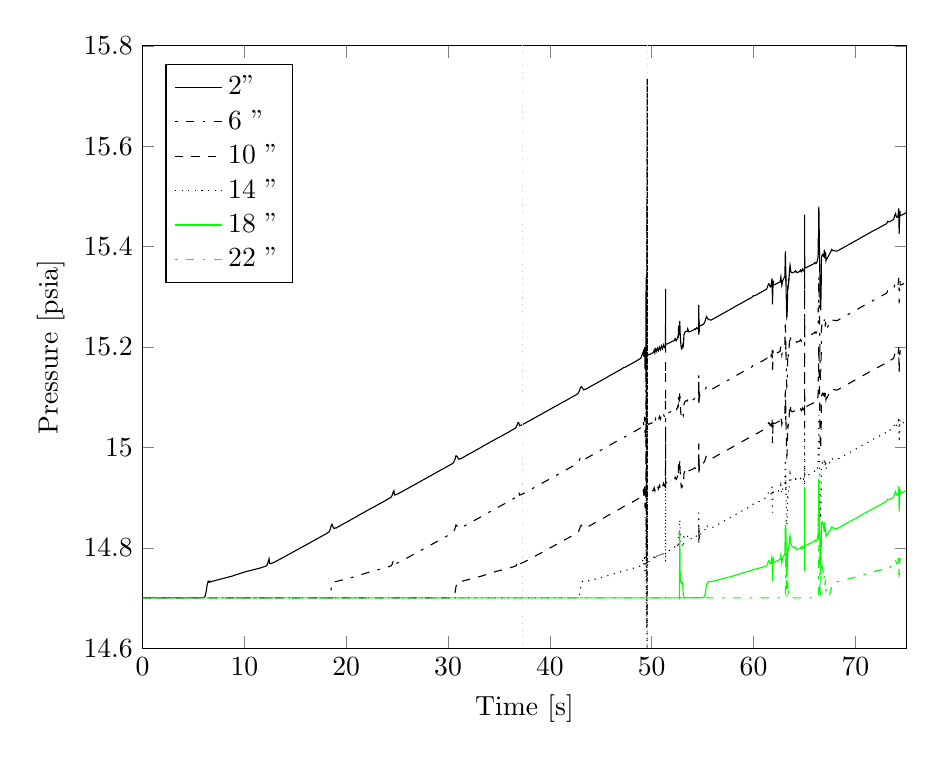
\begin{tikzpicture}

\begin{axis}[%
width=0.8\textwidth,
height=0.630967741935484\textwidth,
scale only axis,
xmin=0,
xmax=75,
xlabel={Time [s]},
ymin=14.6,
ymax=15.8,
ylabel={Pressure [psia]},
legend style={at={(0.03,0.97)},anchor=north west,draw=black,fill=white,legend cell align=left}
]
\addplot [
color=black,
solid
]
table[row sep=crcr]{
0 14.7007818222046\\
9.99999971718069e-10 14.7007818222046\\
2.49999998480632e-09 14.7007818222046\\
4.74999994892755e-09 14.7007818222046\\
8.1250002281763e-09 14.7007818222046\\
1.31874999809156e-08 14.7007818222046\\
2.0781250498203e-08 14.7007818222046\\
3.21718758300449e-08 14.7007818222046\\
4.92578138278077e-08 14.7007818222046\\
7.48867208244519e-08 14.7007818222046\\
1.13330081319418e-07 14.7007818222046\\
1.70995122061868e-07 14.7007818222046\\
2.57492672517401e-07 14.7007818222046\\
3.8723902662241e-07 14.7007818222046\\
5.81858500936505e-07 14.7007818222046\\
8.73787769251066e-07 14.7007818222046\\
1.31168167172291e-06 14.7007818222046\\
1.9685226106958e-06 14.7007827758789\\
2.95378367809462e-06 14.7007827758789\\
4.43167573394021e-06 14.7007827758789\\
6.64851359033491e-06 14.7007827758789\\
9.97376992017962e-06 14.7007837295532\\
1.49616553244414e-05 14.7007846832275\\
2.24434825213393e-05 14.7007856369019\\
3.36662233166862e-05 14.7007865905762\\
5.05003372381907e-05 14.7007884979248\\
7.57515081204474e-05 14.7007904052734\\
0.000113628258986864 14.7007932662964\\
0.000170443381648511 14.700795173645\\
0.000255666091106832 14.7007970809937\\
0.000383500126190484 14.7007970809937\\
0.000575251178815961 14.7007942199707\\
0.000862877757754177 14.7007904052734\\
0.00129431765526533 14.7007865905762\\
0.00194147753063589 14.7007837295532\\
0.00291221728548408 14.700779914856\\
0.00436832662671804 14.7007780075073\\
0.00597004732117057 14.700779914856\\
0.00773194013163447 14.7007827758789\\
0.009670021943748 14.7007837295532\\
0.0118019115179777 14.7007827758789\\
0.0141469910740852 14.7007827758789\\
0.0167265776544809 14.7007827758789\\
0.0195641238242388 14.7007827758789\\
0.0226854234933853 14.7007827758789\\
0.0261188540607691 14.7007827758789\\
0.0298956278711557 14.7007827758789\\
0.0340500771999359 14.7007827758789\\
0.0386199727654457 14.7007827758789\\
0.0436468608677387 14.7007827758789\\
0.0491764321923256 14.7007827758789\\
0.0552589632570744 14.7007827758789\\
0.0619497485458851 14.7007827758789\\
0.0693096145987511 14.7007827758789\\
0.0774054601788521 14.700777053833\\
0.0863108932971954 14.7007865905762\\
0.0961068719625473 14.7007827758789\\
0.106882445514202 14.7007827758789\\
0.118735581636429 14.7007827758789\\
0.13177402317524 14.7007827758789\\
0.146116316318512 14.7007827758789\\
0.161892831325531 14.7007827758789\\
0.179247006773949 14.7007827758789\\
0.198336601257324 14.7007827758789\\
0.21933513879776 14.7007827758789\\
0.242433547973633 14.7007827758789\\
0.267841786146164 14.7007827758789\\
0.29579085111618 14.7007827758789\\
0.32653483748436 14.7007827758789\\
0.360353201627731 14.7007827758789\\
0.397553414106369 14.7007837295532\\
0.438473641872406 14.7007837295532\\
0.483485877513886 14.7007837295532\\
0.532999336719513 14.7007837295532\\
0.587464153766632 14.7007837295532\\
0.647375464439392 14.7007837295532\\
0.71327793598175 14.7007837295532\\
0.7857705950737 14.7007837295532\\
0.865512549877167 14.7007837295532\\
0.953228712081909 14.7007837295532\\
1.04971647262573 14.7007837295532\\
1.14971649646759 14.7007827758789\\
1.24971640110016 14.7007827758789\\
1.34971642494202 14.7007827758789\\
1.44971644878387 14.7007827758789\\
1.54971647262573 14.7007827758789\\
1.64971649646759 14.7007827758789\\
1.74971640110016 14.7007827758789\\
1.84971642494202 14.7007827758789\\
1.94971644878387 14.7007827758789\\
2.04971647262573 14.7007827758789\\
2.1497163772583 14.7007827758789\\
2.24971652030945 14.7007827758789\\
2.34971642494202 14.7007827758789\\
2.44971656799316 14.7007827758789\\
2.54971647262573 14.7007827758789\\
2.6497163772583 14.7007827758789\\
2.74971652030945 14.7007827758789\\
2.84971642494202 14.7007827758789\\
2.94971656799316 14.7007827758789\\
3.04971647262573 14.7007827758789\\
3.1497163772583 14.7007827758789\\
3.24971652030945 14.7007827758789\\
3.34971642494202 14.7007827758789\\
3.44971656799316 14.7007827758789\\
3.54971647262573 14.7007827758789\\
3.6497163772583 14.7007827758789\\
3.74971652030945 14.7007827758789\\
3.84971642494202 14.7007827758789\\
3.94971656799316 14.7007827758789\\
4.04971647262573 14.7007827758789\\
4.1497163772583 14.7007827758789\\
4.24971628189087 14.7007827758789\\
4.3497166633606 14.7007827758789\\
4.44971656799316 14.7007827758789\\
4.54971647262573 14.7007827758789\\
4.6497163772583 14.7007827758789\\
4.74971628189087 14.7007827758789\\
4.8497166633606 14.7007827758789\\
4.94971656799316 14.7007827758789\\
5.04971647262573 14.7007837295532\\
5.1497163772583 14.7007837295532\\
5.24971628189087 14.7007837295532\\
5.3497166633606 14.7007837295532\\
5.44971656799316 14.7007837295532\\
5.54971647262573 14.7007837295532\\
5.6497163772583 14.7007846832275\\
5.74971628189087 14.7007894515991\\
5.8497166633606 14.7008085250854\\
5.94971656799316 14.7009077072144\\
6.04971647262573 14.7014436721802\\
6.1497163772583 14.7040977478027\\
6.24971628189087 14.7128324508667\\
6.3497166633606 14.7271690368652\\
6.44971656799316 14.7334566116333\\
6.54971647262573 14.7314443588257\\
6.6497163772583 14.7334966659546\\
6.74971628189087 14.7322854995728\\
6.8497166633606 14.7336616516113\\
6.94971656799316 14.7335815429688\\
7.04971647262573 14.7345237731934\\
7.1497163772583 14.7347774505615\\
7.24971628189087 14.7354955673218\\
7.3497166633606 14.7358999252319\\
7.44971656799316 14.7365169525146\\
7.54971647262573 14.7369899749756\\
7.6497163772583 14.7375602722168\\
7.74971628189087 14.7380647659302\\
7.8497166633606 14.7386140823364\\
7.94971656799316 14.7391328811646\\
8.04971599578857 14.739673614502\\
8.1497163772583 14.7401990890503\\
8.24971675872803 14.7407350540161\\
8.34971618652344 14.7412633895874\\
8.44971656799316 14.7417974472046\\
8.54971599578857 14.7423276901245\\
8.6497163772583 14.7428607940674\\
8.74971675872803 14.7433929443359\\
8.84971618652344 14.7439479827881\\
8.94971656799316 14.7448120117188\\
9.04971599578857 14.7454252243042\\
9.1497163772583 14.7460870742798\\
9.24971675872803 14.7467250823975\\
9.34971618652344 14.7473707199097\\
9.44971656799316 14.748010635376\\
9.54971599578857 14.7486515045166\\
9.6497163772583 14.7492904663086\\
9.74971675872803 14.7499284744263\\
9.84971618652344 14.7505655288696\\
9.94971656799316 14.751202583313\\
10.0497159957886 14.751838684082\\
10.1497163772583 14.7524747848511\\
10.249716758728 14.7531108856201\\
10.3497161865234 14.7537298202515\\
10.4497165679932 14.7540988922119\\
10.5497159957886 14.7545909881592\\
10.6497163772583 14.7551307678223\\
10.749716758728 14.755651473999\\
10.8497161865234 14.7561731338501\\
10.9497165679932 14.756688117981\\
11.0497159957886 14.7571992874146\\
11.1497163772583 14.7577028274536\\
11.249716758728 14.7581987380981\\
11.3497161865234 14.7586870193481\\
11.4497165679932 14.7591991424561\\
11.5497159957886 14.7598543167114\\
11.6497163772583 14.7605504989624\\
11.749716758728 14.7611818313599\\
11.8497161865234 14.7618141174316\\
11.9497165679932 14.7624731063843\\
12.0497159957886 14.7631711959839\\
12.1497163772583 14.7639303207397\\
12.249716758728 14.7665214538574\\
12.3471450805664 14.7732496261597\\
12.4250917434692 14.7781705856323\\
12.4879579544067 14.768609046936\\
12.557110786438 14.7686433792114\\
12.6331787109375 14.7690782546997\\
12.7168531417847 14.7695474624634\\
12.808895111084 14.7702302932739\\
12.9088954925537 14.7711057662964\\
13.0088949203491 14.7721309661865\\
13.1088953018188 14.7731733322144\\
13.2088947296143 14.7742366790771\\
13.308895111084 14.7753143310547\\
13.4088954925537 14.7763986587524\\
13.5088949203491 14.777494430542\\
13.6088953018188 14.7785978317261\\
13.7088947296143 14.7797069549561\\
13.808895111084 14.780816078186\\
13.9088954925537 14.781925201416\\
14.0088949203491 14.783034324646\\
14.1088953018188 14.784143447876\\
14.2088947296143 14.7852535247803\\
14.308895111084 14.7863636016846\\
14.4088954925537 14.7874736785889\\
14.5088949203491 14.7885837554932\\
14.6088953018188 14.7896947860718\\
14.7088947296143 14.7908058166504\\
14.808895111084 14.7919178009033\\
14.9088954925537 14.7930297851563\\
15.0088949203491 14.7941417694092\\
15.1088953018188 14.7952537536621\\
15.2088947296143 14.7963666915894\\
15.308895111084 14.7974805831909\\
15.4088954925537 14.7986001968384\\
15.5088949203491 14.7997035980225\\
15.6088953018188 14.8008260726929\\
15.7088947296143 14.8019437789917\\
15.808895111084 14.8030633926392\\
15.9088954925537 14.8041830062866\\
16.0088958740234 14.8053026199341\\
16.1088943481445 14.8064222335815\\
16.2088947296143 14.8075428009033\\
16.308895111084 14.8086624145508\\
16.4088954925537 14.8097829818726\\
16.5088958740234 14.8109035491943\\
16.6088943481445 14.8120241165161\\
16.7088947296143 14.8131446838379\\
16.808895111084 14.814266204834\\
16.9088954925537 14.8153867721558\\
17.0088958740234 14.8165082931519\\
17.1088943481445 14.8176298141479\\
17.2088947296143 14.818751335144\\
17.308895111084 14.8198738098145\\
17.4088954925537 14.8209953308105\\
17.5088958740234 14.822117805481\\
17.6088943481445 14.8232402801514\\
17.7088947296143 14.8243627548218\\
17.808895111084 14.8254852294922\\
17.9088954925537 14.8266096115112\\
18.0088958740234 14.8277368545532\\
18.1088943481445 14.8288841247559\\
18.2088947296143 14.830132484436\\
18.308895111084 14.8319272994995\\
18.4088954925537 14.8359346389771\\
18.5088958740234 14.8431234359741\\
18.6088943481445 14.8468885421753\\
18.7088947296143 14.8412246704102\\
18.808895111084 14.8385257720947\\
18.9088954925537 14.8396024703979\\
19.0088958740234 14.8392372131348\\
19.1088943481445 14.8409767150879\\
19.2088947296143 14.8416633605957\\
19.308895111084 14.8430795669556\\
19.4088954925537 14.8440103530884\\
19.5088958740234 14.8452653884888\\
19.6088943481445 14.8463039398193\\
19.7088947296143 14.8474884033203\\
19.808895111084 14.848575592041\\
19.9088954925537 14.8497276306152\\
20.0088958740234 14.8508358001709\\
20.1088943481445 14.8519744873047\\
20.2088947296143 14.8530921936035\\
20.308895111084 14.8542242050171\\
20.4088954925537 14.8553476333618\\
20.5088958740234 14.8564767837524\\
20.6088943481445 14.8576021194458\\
20.7088947296143 14.8587303161621\\
20.808895111084 14.8598566055298\\
20.9088954925537 14.8609848022461\\
21.0088958740234 14.8621110916138\\
21.1088943481445 14.8633079528809\\
21.2088947296143 14.8647031784058\\
21.308895111084 14.8657855987549\\
21.4088954925537 14.8669328689575\\
21.5088958740234 14.8680543899536\\
21.6088943481445 14.8691864013672\\
21.7088947296143 14.8703145980835\\
21.808895111084 14.8714447021484\\
21.9088954925537 14.8725738525391\\
22.0088958740234 14.8737049102783\\
22.1088943481445 14.8748359680176\\
22.2088947296143 14.8759670257568\\
22.308895111084 14.8770990371704\\
22.4088954925537 14.878231048584\\
22.5088958740234 14.8793640136719\\
22.6088943481445 14.8804807662964\\
22.7088947296143 14.8813285827637\\
22.808895111084 14.8824396133423\\
22.9088954925537 14.8835592269897\\
23.0088958740234 14.8846778869629\\
23.1088943481445 14.8857955932617\\
23.2088947296143 14.8869123458862\\
23.308895111084 14.8880281448364\\
23.4088954925537 14.889142036438\\
23.5088958740234 14.8902549743652\\
23.6088943481445 14.8913650512695\\
23.7088947296143 14.8925113677979\\
23.808895111084 14.8937644958496\\
23.9088954925537 14.894998550415\\
24.0088958740234 14.8961601257324\\
24.1088943481445 14.8973197937012\\
24.2088947296143 14.8984975814819\\
24.308895111084 14.8997011184692\\
24.4088954925537 14.9009475708008\\
24.5088958740234 14.9045486450195\\
24.6048831939697 14.910834312439\\
24.681676864624 14.9136018753052\\
24.7464084625244 14.9051694869995\\
24.8176136016846 14.9055252075195\\
24.895938873291 14.9060869216919\\
24.9820976257324 14.9067459106445\\
25.0768718719482 14.9075870513916\\
25.176872253418 14.9086112976074\\
25.2768707275391 14.9097194671631\\
25.3768711090088 14.9108257293701\\
25.4768714904785 14.911937713623\\
25.5768718719482 14.9130535125732\\
25.676872253418 14.9141712188721\\
25.7768707275391 14.9152879714966\\
25.8768711090088 14.9164094924927\\
25.9768714904785 14.9175319671631\\
26.0768718719482 14.9186611175537\\
26.176872253418 14.9197883605957\\
26.2768707275391 14.920916557312\\
26.3768711090088 14.9220447540283\\
26.4768714904785 14.9231729507446\\
26.5768718719482 14.9243001937866\\
26.676872253418 14.9254283905029\\
26.7768707275391 14.9265565872192\\
26.8768711090088 14.9276838302612\\
26.9768714904785 14.9288120269775\\
27.0768718719482 14.9299402236938\\
27.176872253418 14.9310674667358\\
27.2768707275391 14.9321956634521\\
27.3768711090088 14.9333238601685\\
27.4768714904785 14.9344511032104\\
27.5768718719482 14.9355792999268\\
27.676872253418 14.9367065429688\\
27.7768707275391 14.9378347396851\\
27.8768711090088 14.9389629364014\\
27.9768714904785 14.9400901794434\\
28.0768718719482 14.9412183761597\\
28.176872253418 14.9423456192017\\
28.2768707275391 14.9434804916382\\
28.3768711090088 14.9445905685425\\
28.4768714904785 14.9457235336304\\
28.5768718719482 14.946849822998\\
28.676872253418 14.9479780197144\\
28.7768707275391 14.9491062164307\\
28.8768711090088 14.950234413147\\
28.9768714904785 14.9513626098633\\
29.0768718719482 14.9524898529053\\
29.176872253418 14.9536180496216\\
29.2768707275391 14.9547462463379\\
29.3768711090088 14.9558744430542\\
29.4768714904785 14.9570026397705\\
29.5768718719482 14.9581298828125\\
29.676872253418 14.9592580795288\\
29.7768707275391 14.9603862762451\\
29.8768711090088 14.9615144729614\\
29.9768714904785 14.9626426696777\\
30.0768718719482 14.963770866394\\
30.176872253418 14.964900970459\\
30.2768707275391 14.9660387039185\\
30.3768711090088 14.9672107696533\\
30.4768714904785 14.9685831069946\\
30.5768718719482 14.9709510803223\\
30.676872253418 14.9764404296875\\
30.7768707275391 14.9835319519043\\
30.8768711090088 14.9819793701172\\
30.9768714904785 14.9787912368774\\
31.0768718719482 14.9764232635498\\
31.176872253418 14.9774360656738\\
31.2768707275391 14.9776411056519\\
31.3768711090088 14.9792537689209\\
31.4768714904785 14.9800567626953\\
31.5768718719482 14.9814014434814\\
31.676872253418 14.982385635376\\
31.7768707275391 14.9836101531982\\
31.8768711090088 14.9846744537354\\
31.9768714904785 14.9858465194702\\
32.0768699645996 14.986946105957\\
32.176872253418 14.988094329834\\
32.2768707275391 14.9892101287842\\
32.3768730163574 14.9903469085693\\
32.4768714904785 14.9914693832397\\
32.5768699645996 14.9926023483276\\
32.676872253418 14.9937286376953\\
32.7768707275391 14.9948596954346\\
32.8768730163574 14.9959878921509\\
32.9768714904785 14.9971179962158\\
33.0768699645996 14.9982461929321\\
33.176872253418 14.9993753433228\\
33.2768707275391 15.0005044937134\\
33.3768730163574 15.0018339157104\\
33.4768714904785 15.0030736923218\\
33.5768699645996 15.0041904449463\\
33.676872253418 15.0053262710571\\
33.7768707275391 15.0064544677734\\
33.8768730163574 15.0075855255127\\
33.9768714904785 15.0087156295776\\
34.0768699645996 15.0098466873169\\
34.176872253418 15.0109786987305\\
34.2768707275391 15.0121097564697\\
34.3768730163574 15.0132417678833\\
34.4768714904785 15.0143747329712\\
34.5768699645996 15.0155076980591\\
34.676872253418 15.0166416168213\\
34.7768707275391 15.0177755355835\\
34.8768730163574 15.0188503265381\\
34.9768714904785 15.0196676254272\\
35.0768699645996 15.0208778381348\\
35.176872253418 15.0219659805298\\
35.2768707275391 15.0230979919434\\
35.3768730163574 15.0242118835449\\
35.4768714904785 15.0253314971924\\
35.5768699645996 15.0264482498169\\
35.676872253418 15.0275640487671\\
35.7768707275391 15.0286779403687\\
35.8768730163574 15.0297899246216\\
35.9768714904785 15.0309648513794\\
36.0768699645996 15.0322227478027\\
36.176872253418 15.0334167480469\\
36.2768707275391 15.034571647644\\
36.3768730163574 15.0357360839844\\
36.4768714904785 15.036919593811\\
36.5768699645996 15.0381326675415\\
36.676872253418 15.0393943786621\\
36.7768707275391 15.0450391769409\\
36.8673248291016 15.049633026123\\
36.9396858215332 15.0495882034302\\
37.0192794799805 15.043267250061\\
37.1068305969238 15.0439186096191\\
37.2031402587891 15.0445747375488\\
37.3031425476074 15.0454931259155\\
37.4031410217285 15.046555519104\\
37.5031433105469 15.0476732254028\\
37.603141784668 15.0487785339355\\
37.7031402587891 15.0498905181885\\
37.8031425476074 15.0510053634644\\
37.9031410217285 15.0521259307861\\
38.0031433105469 15.053240776062\\
38.103141784668 15.0543622970581\\
38.2031402587891 15.0554847717285\\
38.3031425476074 15.0566120147705\\
38.4031410217285 15.0577402114868\\
38.5031433105469 15.0588684082031\\
38.603141784668 15.0599966049194\\
38.7031402587891 15.0611248016357\\
38.8031425476074 15.0622529983521\\
38.9031410217285 15.0633811950684\\
39.0031433105469 15.064510345459\\
39.103141784668 15.0656385421753\\
39.2031402587891 15.0667657852173\\
39.3031425476074 15.0678939819336\\
39.4031410217285 15.0690221786499\\
39.5031433105469 15.0701503753662\\
39.603141784668 15.0712785720825\\
39.7031402587891 15.0724067687988\\
39.8031425476074 15.0735349655151\\
39.9031410217285 15.0746631622314\\
40.0031433105469 15.0757913589478\\
40.103141784668 15.0769195556641\\
40.2031402587891 15.0780477523804\\
40.3031425476074 15.0791759490967\\
40.4031410217285 15.080304145813\\
40.5031433105469 15.0814323425293\\
40.603141784668 15.0825595855713\\
40.7031402587891 15.0836877822876\\
40.8031425476074 15.0848159790039\\
40.9031410217285 15.0859508514404\\
41.0031433105469 15.0870609283447\\
41.103141784668 15.0881948471069\\
41.2031402587891 15.0893211364746\\
41.3031425476074 15.0904502868652\\
41.4031410217285 15.0915775299072\\
41.5031433105469 15.0927066802979\\
41.603141784668 15.0938348770142\\
41.7031402587891 15.0949630737305\\
41.8031425476074 15.0960912704468\\
41.9031410217285 15.0972194671631\\
42.0031433105469 15.0983476638794\\
42.103141784668 15.0994758605957\\
42.2031402587891 15.100604057312\\
42.3031425476074 15.1017332077026\\
42.4031410217285 15.1028623580933\\
42.5031433105469 15.1039972305298\\
42.603141784668 15.1051578521729\\
42.7031402587891 15.106463432312\\
42.8031425476074 15.1085205078125\\
42.9031410217285 15.1132192611694\\
43.0031433105469 15.1198301315308\\
43.103141784668 15.1210536956787\\
43.2031402587891 15.1182489395142\\
43.3031425476074 15.1148796081543\\
43.4031410217285 15.1154232025146\\
43.5031433105469 15.1156797409058\\
43.603141784668 15.1171436309814\\
43.7031402587891 15.1179189682007\\
43.8031425476074 15.1194105148315\\
43.9031410217285 15.1202983856201\\
44.0031433105469 15.1215867996216\\
44.103141784668 15.1226081848145\\
44.2031402587891 15.1238079071045\\
44.3031425476074 15.1248893737793\\
44.4031410217285 15.1260499954224\\
44.5031433105469 15.1271572113037\\
44.603141784668 15.1282997131348\\
44.7031402587891 15.1294183731079\\
44.8031425476074 15.1305532455444\\
44.9031410217285 15.1316776275635\\
45.0031433105469 15.1328096389771\\
45.103141784668 15.1339359283447\\
45.2031402587891 15.1350660324097\\
45.3031425476074 15.136194229126\\
45.4031410217285 15.1373233795166\\
45.5031433105469 15.1384515762329\\
45.603141784668 15.139723777771\\
45.7031402587891 15.1410293579102\\
45.8031425476074 15.1421155929565\\
45.9031410217285 15.1432571411133\\
46.0031433105469 15.1443815231323\\
46.103141784668 15.1455116271973\\
46.2031402587891 15.1466398239136\\
46.3031425476074 15.1477689743042\\
46.4031410217285 15.1488981246948\\
46.5031433105469 15.1500263214111\\
46.603141784668 15.1511554718018\\
46.7031402587891 15.1522836685181\\
46.8031425476074 15.1534128189087\\
46.9031410217285 15.154541015625\\
47.0031433105469 15.1556701660156\\
47.103141784668 15.1567935943604\\
47.2031402587891 15.1587295532227\\
47.3031425476074 15.1590728759766\\
47.4031410217285 15.1598958969116\\
47.5031433105469 15.1610918045044\\
47.603141784668 15.162181854248\\
47.7031402587891 15.163311958313\\
47.8031425476074 15.1644258499146\\
47.9031410217285 15.1655435562134\\
48.0031433105469 15.1666584014893\\
48.103141784668 15.1677722930908\\
48.2031402587891 15.1689252853394\\
48.3031425476074 15.1701030731201\\
48.4031410217285 15.1714162826538\\
48.5031433105469 15.1725482940674\\
48.603141784668 15.1736869812012\\
48.7031402587891 15.1748695373535\\
48.8031425476074 15.1760702133179\\
48.9031410217285 15.1773176193237\\
49.0031433105469 15.1813631057739\\
49.098030090332 15.186785697937\\
49.1739387512207 15.1910095214844\\
49.2346649169922 15.1802492141724\\
49.3014602661133 15.1998834609985\\
49.3450546264648 15.1551971435547\\
49.3930053710938 15.1706562042236\\
49.4215202331543 15.193733215332\\
49.4451713562012 15.3380928039551\\
49.47119140625 15.055549621582\\
49.4998092651367 15.1796255111694\\
49.515323638916 15.1865968704224\\
49.5276222229004 15.4837913513184\\
49.5411529541016 14.9221239089966\\
49.5560340881348 15.1116857528687\\
49.5575561523438 15.7338838577271\\
49.5592269897461 15.3602809906006\\
49.5610656738281 15.1738147735596\\
49.5630912780762 15.1993160247803\\
49.565315246582 15.2013034820557\\
49.5677642822266 15.1970310211182\\
49.5704574584961 15.1936655044556\\
49.5734214782715 15.1910648345947\\
49.5766792297363 15.1890506744385\\
49.5791168212891 15.1878967285156\\
49.5817947387695 15.1869592666626\\
49.5847434997559 15.1862087249756\\
49.5879859924316 15.1856250762939\\
49.591552734375 15.1851825714111\\
49.5954742431641 15.1848583221436\\
49.5997886657715 15.1846294403076\\
49.6045341491699 15.1844730377197\\
49.6097564697266 15.1843709945679\\
49.6155014038086 15.1843090057373\\
49.6218185424805 15.1842756271362\\
49.6287651062012 15.1842632293701\\
49.6364097595215 15.1842651367188\\
49.6448211669922 15.1842803955078\\
49.6540679931641 15.18430519104\\
49.6642456054688 15.1843414306641\\
49.6754379272461 15.1844673156738\\
49.6877479553223 15.184681892395\\
49.7012901306152 15.1848411560059\\
49.7161865234375 15.1849393844604\\
49.7325744628906 15.1849765777588\\
49.7505989074707 15.1849966049194\\
49.7704238891602 15.1850490570068\\
49.792236328125 15.1853446960449\\
49.8162269592285 15.1856250762939\\
49.8426170349121 15.1858415603638\\
49.8716468811035 15.1860265731812\\
49.9035758972168 15.1862478256226\\
49.9387016296387 15.1865177154541\\
49.9773406982422 15.1868839263916\\
50.0198440551758 15.1873455047607\\
50.066593170166 15.1879167556763\\
50.1180229187012 15.1886320114136\\
50.1745910644531 15.1894807815552\\
50.23681640625 15.1942272186279\\
50.3052673339844 15.1885976791382\\
50.3805618286133 15.1955699920654\\
50.4633865356445 15.1914644241333\\
50.5544929504395 15.1978197097778\\
50.6544914245605 15.1927089691162\\
50.7544898986816 15.1998929977417\\
50.8544921875 15.1946296691895\\
50.9544906616211 15.2021837234497\\
51.0544929504395 15.1967191696167\\
51.1544914245605 15.2043790817261\\
51.2544898986816 15.1989612579346\\
51.3544921875 15.2012796401978\\
51.3568458557129 15.3158397674561\\
51.359432220459 15.2306413650513\\
51.3622817993164 15.1889343261719\\
51.3654136657715 15.1953868865967\\
51.3688583374023 15.2051019668579\\
51.3726463317871 15.206883430481\\
51.3768157958984 15.2060050964355\\
51.3814010620117 15.2056035995483\\
51.3864479064941 15.205605506897\\
51.3919944763184 15.2056283950806\\
51.3980979919434 15.2056255340576\\
51.4048118591309 15.2056226730347\\
51.4121971130371 15.2056264877319\\
51.4203224182129 15.2056398391724\\
51.4292602539063 15.2056617736816\\
51.4390869140625 15.2056941986084\\
51.4499015808105 15.2057399749756\\
51.4617958068848 15.2058000564575\\
51.4748802185059 15.2058763504028\\
51.4892692565918 15.2059707641602\\
51.5051002502441 15.2060852050781\\
51.522518157959 15.2062206268311\\
51.5416717529297 15.2063808441162\\
51.562744140625 15.2065658569336\\
51.5859222412109 15.2067785263062\\
51.6114196777344 15.2070207595825\\
51.6394653320313 15.2072925567627\\
51.6703147888184 15.2075986862183\\
51.7042503356934 15.2079391479492\\
51.7415771484375 15.2083177566528\\
51.7826385498047 15.2087364196777\\
51.827808380127 15.2091979980469\\
51.8774948120117 15.2097072601318\\
51.9321479797363 15.2102670669556\\
51.9922637939453 15.2108840942383\\
52.0583953857422 15.2115631103516\\
52.1311378479004 15.212308883667\\
52.2111587524414 15.2131586074829\\
52.2991790771484 15.2166986465454\\
52.3959999084473 15.2122888565063\\
52.4959983825684 15.2162237167358\\
52.5960006713867 15.2233877182007\\
52.6160011291504 15.2175693511963\\
52.6228942871094 15.2351388931274\\
52.6304740905762 15.2396717071533\\
52.637622833252 15.2409086227417\\
52.6454811096191 15.2411556243896\\
52.6532897949219 15.240891456604\\
52.6618766784668 15.2379388809204\\
52.6713256835938 15.2349061965942\\
52.6817169189453 15.2345190048218\\
52.6931457519531 15.232684135437\\
52.7057189941406 15.2282514572144\\
52.7195510864258 15.2291049957275\\
52.7347640991211 15.2381162643433\\
52.7514991760254 15.251898765564\\
52.7699089050293 15.2411470413208\\
52.7901573181152 15.2278718948364\\
52.8124351501465 15.2203044891357\\
52.8369369506836 15.2122440338135\\
52.8638877868652 15.204083442688\\
52.8935356140137 15.1988039016724\\
52.9261474609375 15.1959705352783\\
52.9620208740234 15.1962118148804\\
53.0014839172363 15.2002544403076\\
53.0448913574219 15.2043762207031\\
53.0926399230957 15.2019996643066\\
53.1261940002441 15.2084064483643\\
53.1631088256836 15.2250728607178\\
53.1971549987793 15.2256288528442\\
53.2346038818359 15.2281303405762\\
53.2757987976074 15.2299757003784\\
53.3211135864258 15.2309226989746\\
53.3709602355957 15.2312850952148\\
53.4181785583496 15.2309350967407\\
53.4612884521484 15.230842590332\\
53.4995498657227 15.2311086654663\\
53.5327682495117 15.2360734939575\\
53.5693130493164 15.2341794967651\\
53.6095085144043 15.231861114502\\
53.6537246704102 15.230170249939\\
53.7023620605469 15.2305145263672\\
53.7558631896973 15.2309226989746\\
53.8147125244141 15.2312860488892\\
53.8794479370117 15.2318029403687\\
53.9506568908691 15.2324628829956\\
54.0289878845215 15.2331943511963\\
54.1151542663574 15.2340221405029\\
54.2099342346191 15.2361001968384\\
54.3099327087402 15.2347192764282\\
54.4099311828613 15.2384662628174\\
54.5099334716797 15.2368202209473\\
54.6099319458008 15.2386226654053\\
54.6148452758789 15.2837533950806\\
54.6202507019043 15.2247676849365\\
54.6261940002441 15.2574901580811\\
54.6327362060547 15.2257776260376\\
54.6399269104004 15.2558479309082\\
54.6478385925293 15.2280359268188\\
54.6565437316895 15.2537355422974\\
54.6661186218262 15.2300968170166\\
54.6766510009766 15.2391567230225\\
54.6824378967285 15.2456026077271\\
54.6888046264648 15.2419948577881\\
54.6958045959473 15.2416915893555\\
54.7035064697266 15.2417936325073\\
54.7119827270508 15.2418432235718\\
54.7213020324707 15.2418947219849\\
54.7315559387207 15.2419576644897\\
54.7428321838379 15.2420320510864\\
54.7552375793457 15.2421236038208\\
54.7688827514648 15.2422285079956\\
54.7838935852051 15.2423505783081\\
54.800407409668 15.2424917221069\\
54.8185691833496 15.242654800415\\
54.8385467529297 15.2428407669067\\
54.8605270385742 15.243052482605\\
54.8847007751465 15.2432889938354\\
54.9112930297852 15.2435665130615\\
54.940544128418 15.2438774108887\\
54.9727210998535 15.244236946106\\
55.008113861084 15.2446613311768\\
55.0470504760742 15.245189666748\\
55.0898742675781 15.2459030151367\\
55.1369857788086 15.2469835281372\\
55.1888084411621 15.2488088607788\\
55.2458114624023 15.2520313262939\\
55.3085136413574 15.2566051483154\\
55.3774871826172 15.2605056762695\\
55.4533576965332 15.2577028274536\\
55.5368156433105 15.2554473876953\\
55.6286201477051 15.2545604705811\\
55.7286186218262 15.2540254592896\\
55.8286209106445 15.2535276412964\\
55.9286193847656 15.254768371582\\
56.0286178588867 15.2557430267334\\
56.1286201477051 15.2571449279785\\
56.2286186218262 15.258092880249\\
56.3286209106445 15.2593393325806\\
56.4286193847656 15.2603893280029\\
56.5286178588867 15.2615690231323\\
56.6286201477051 15.2626628875732\\
56.7286186218262 15.2638139724731\\
56.8286209106445 15.2649602890015\\
56.9286193847656 15.266077041626\\
57.0286178588867 15.2671804428101\\
57.1286201477051 15.2683191299438\\
57.2286186218262 15.2694387435913\\
57.3286209106445 15.2705726623535\\
57.4286193847656 15.2716970443726\\
57.5286178588867 15.2728281021118\\
57.6286201477051 15.2739543914795\\
57.7286186218262 15.2750844955444\\
57.8286209106445 15.2762117385864\\
57.9286193847656 15.2773418426514\\
58.0286178588867 15.2787885665894\\
58.1286201477051 15.2798681259155\\
58.2286186218262 15.2810182571411\\
58.3286209106445 15.2821378707886\\
58.4286193847656 15.2832689285278\\
58.5286178588867 15.2843961715698\\
58.6286201477051 15.2855253219604\\
58.7286186218262 15.2866535186768\\
58.8286209106445 15.2877817153931\\
58.9286193847656 15.2889108657837\\
59.0286178588867 15.2900390625\\
59.1286201477051 15.2911701202393\\
59.2286186218262 15.2922983169556\\
59.3286209106445 15.2934274673462\\
59.4286193847656 15.2945556640625\\
59.5286178588867 15.2955083847046\\
59.6286201477051 15.2964887619019\\
59.7286186218262 15.2976522445679\\
59.8286209106445 15.2987480163574\\
59.9143104553223 15.3011493682861\\
60 15.3022813796997\\
60.0942611694336 15.3021421432495\\
60.1942596435547 15.3029870986938\\
60.2942581176758 15.3041391372681\\
60.3942604064941 15.3052577972412\\
60.4942588806152 15.3063888549805\\
60.5942611694336 15.3075199127197\\
60.6942596435547 15.3086557388306\\
60.7942581176758 15.3098049163818\\
60.8942604064941 15.3109512329102\\
60.9942588806152 15.312108039856\\
61.0942611694336 15.3132829666138\\
61.1942596435547 15.3144845962524\\
61.2942581176758 15.3157434463501\\
61.3942604064941 15.321587562561\\
61.4835205078125 15.3258171081543\\
61.5549278259277 15.3251113891602\\
61.6334800720215 15.3196935653687\\
61.7198829650879 15.3203210830688\\
61.8149299621582 15.3367099761963\\
61.8549957275391 15.2851409912109\\
61.8990707397461 15.3168239593506\\
61.9192581176758 15.3288249969482\\
61.9358787536621 15.3320579528809\\
61.9541664123535 15.3236618041992\\
61.9742813110352 15.3236713409424\\
61.9964065551758 15.3238325119019\\
62.0207443237305 15.3240013122559\\
62.0475158691406 15.3242092132568\\
62.0769653320313 15.3244562149048\\
62.1093559265137 15.324746131897\\
62.1449890136719 15.3250799179077\\
62.1841850280762 15.3254594802856\\
62.2273025512695 15.325888633728\\
62.274730682373 15.3263683319092\\
62.3269004821777 15.3269014358521\\
62.3842887878418 15.3274908065796\\
62.4474143981934 15.3281402587891\\
62.5168533325195 15.3288536071777\\
62.5932350158691 15.3296384811401\\
62.6772575378418 15.3396949768066\\
62.7696800231934 15.3228168487549\\
62.8696823120117 15.3325929641724\\
62.9696807861328 15.3367834091187\\
63.0696792602539 15.3411664962769\\
63.1196823120117 15.3907136917114\\
63.1572036743164 15.3497362136841\\
63.1601943969727 15.3309259414673\\
63.1634902954102 15.3392190933228\\
63.1671104431152 15.3568449020386\\
63.1710968017578 15.3588838577271\\
63.175479888916 15.3461332321167\\
63.1803016662598 15.3361902236938\\
63.185604095459 15.3247270584106\\
63.1914367675781 15.3136568069458\\
63.1978569030762 15.3068113327026\\
63.2049140930176 15.3020153045654\\
63.2126808166504 15.2971162796021\\
63.2212219238281 15.2908229827881\\
63.2306175231934 15.2818756103516\\
63.2409515380859 15.2716054916382\\
63.2523231506348 15.2633075714111\\
63.2648277282715 15.2594404220581\\
63.2785835266113 15.2605962753296\\
63.2937164306641 15.2666864395142\\
63.310359954834 15.2788066864014\\
63.328670501709 15.2962188720703\\
63.3488121032715 15.3215398788452\\
63.3709678649902 15.3141469955444\\
63.395336151123 15.3186225891113\\
63.4221420288086 15.3311576843262\\
63.4516296386719 15.3289785385132\\
63.4840698242188 15.3344812393188\\
63.4999580383301 15.3429727554321\\
63.5174407958984 15.347864151001\\
63.5366668701172 15.352068901062\\
63.5578193664551 15.3585720062256\\
63.5810852050781 15.3631057739258\\
63.6066780090332 15.359956741333\\
63.6348304748535 15.3532676696777\\
63.6657981872559 15.3498363494873\\
63.6998634338379 15.34876537323\\
63.7373313903809 15.348352432251\\
63.7785491943359 15.3478736877441\\
63.8238906860352 15.3477048873901\\
63.8737640380859 15.348180770874\\
63.9286231994629 15.3492069244385\\
63.9762001037598 15.3493194580078\\
64.0218276977539 15.3493127822876\\
64.0647964477539 15.3504915237427\\
64.112060546875 15.352147102356\\
64.1640548706055 15.3508062362671\\
64.2212448120117 15.3481941223145\\
64.2841567993164 15.3484973907471\\
64.3533554077148 15.3490533828735\\
64.4294738769531 15.3495655059814\\
64.5132064819336 15.3502960205078\\
64.6053161621094 15.3531799316406\\
64.7053146362305 15.3500699996948\\
64.8053131103516 15.3554763793945\\
64.9053115844727 15.3520078659058\\
65.0053176879883 15.354395866394\\
65.0079345703125 15.4639558792114\\
65.0108184814453 15.3271446228027\\
65.0139923095703 15.3169078826904\\
65.0165023803711 15.3648796081543\\
65.0192642211914 15.3793926239014\\
65.0223007202148 15.3610067367554\\
65.025634765625 15.3563375473022\\
65.0293121337891 15.3573131561279\\
65.0333557128906 15.3577079772949\\
65.0377960205078 15.357684135437\\
65.0426864624023 15.3576622009277\\
65.0480651855469 15.3576612472534\\
65.0539855957031 15.357666015625\\
65.0604934692383 15.3576745986938\\
65.0676498413086 15.3576898574829\\
65.0755233764648 15.3577127456665\\
65.0841903686523 15.3577442169189\\
65.0937194824219 15.3577861785889\\
65.1042022705078 15.3578386306763\\
65.1157302856445 15.3579053878784\\
65.1284103393555 15.3579864501953\\
65.1423645019531 15.3580846786499\\
65.1577072143555 15.3582010269165\\
65.1745910644531 15.3583374023438\\
65.1931610107422 15.3584957122803\\
65.2135848999023 15.358678817749\\
65.2360534667969 15.35888671875\\
65.2607727050781 15.3591232299805\\
65.287956237793 15.3593883514404\\
65.3178634643555 15.3596849441528\\
65.3507614135742 15.3600158691406\\
65.3869476318359 15.3603830337524\\
65.4267501831055 15.3607883453369\\
65.4705352783203 15.3612356185913\\
65.5186996459961 15.3617296218872\\
65.5716781616211 15.3622722625732\\
65.6299591064453 15.3628702163696\\
65.6940612792969 15.3635272979736\\
65.7645797729492 15.3642511367798\\
65.8421478271484 15.3650465011597\\
65.9274749755859 15.3659219741821\\
66.0213317871094 15.3685941696167\\
66.1213302612305 15.3660669326782\\
66.2213287353516 15.3691816329956\\
66.3213272094727 15.378080368042\\
66.3413314819336 15.3859300613403\\
66.3490600585938 15.4133529663086\\
66.3565673828125 15.4173974990845\\
66.3648223876953 15.4138975143433\\
66.3727111816406 15.4104156494141\\
66.3813858032227 15.4161310195923\\
66.3909301757813 15.4455499649048\\
66.4014358520508 15.4762687683105\\
66.4129867553711 15.4794082641602\\
66.4256896972656 15.4570236206055\\
66.4396667480469 15.4365787506104\\
66.4550399780273 15.4139404296875\\
66.4719543457031 15.3901805877686\\
66.4905548095703 15.3658885955811\\
66.5110244750977 15.3353652954102\\
66.5335311889648 15.2999982833862\\
66.5504302978516 15.2850399017334\\
66.5690307617188 15.2758960723877\\
66.5894775390625 15.2730531692505\\
66.6119766235352 15.2928838729858\\
66.6367263793945 15.3197946548462\\
66.663948059082 15.3735342025757\\
66.6938934326172 15.3803434371948\\
66.7268295288086 15.3830423355103\\
66.7630615234375 15.3843870162964\\
66.8029174804688 15.3834896087646\\
66.8467636108398 15.3816804885864\\
66.8949890136719 15.3803443908691\\
66.9480361938477 15.3936891555786\\
67.0063934326172 15.3768825531006\\
67.0705795288086 15.3887996673584\\
67.111457824707 15.372163772583\\
67.1564254760742 15.3757543563843\\
67.1973037719727 15.3756227493286\\
67.2330703735352 15.3765630722046\\
67.2724151611328 15.3781366348267\\
67.3156967163086 15.3802709579468\\
67.3633117675781 15.3817958831787\\
67.4156799316406 15.3833484649658\\
67.4732894897461 15.3856945037842\\
67.5366516113281 15.3882837295532\\
67.6063613891602 15.3914194107056\\
67.6830368041992 15.3942546844482\\
67.7673797607422 15.3919649124146\\
67.8601531982422 15.3919610977173\\
67.9601516723633 15.3914823532104\\
68.0601577758789 15.3912115097046\\
68.16015625 15.3908996582031\\
68.2601547241211 15.3916702270508\\
68.3601531982422 15.3928184509277\\
68.4601516723633 15.3940868377686\\
68.5601577758789 15.3951177597046\\
68.66015625 15.3963060379028\\
68.7601547241211 15.3973922729492\\
68.8601531982422 15.3985471725464\\
68.9601516723633 15.3996572494507\\
69.0601577758789 15.4007978439331\\
69.16015625 15.4019184112549\\
69.2601547241211 15.4030513763428\\
69.3601531982422 15.4041767120361\\
69.4601516723633 15.4053068161011\\
69.5601577758789 15.4064340591431\\
69.66015625 15.4075632095337\\
69.7601547241211 15.40869140625\\
69.8601531982422 15.4098196029663\\
69.9601516723633 15.4109477996826\\
70.0601577758789 15.4120769500732\\
70.16015625 15.4132051467896\\
70.2601547241211 15.4143447875977\\
70.3601531982422 15.4155149459839\\
70.4601516723633 15.4169282913208\\
70.5601577758789 15.4179801940918\\
70.66015625 15.4191312789917\\
70.7601547241211 15.4202537536621\\
70.8601531982422 15.4213848114014\\
70.9601516723633 15.4225130081177\\
71.0601577758789 15.4236421585083\\
71.16015625 15.4247703552246\\
71.2601547241211 15.4258995056152\\
71.3601531982422 15.4270277023315\\
71.4601516723633 15.4281568527222\\
71.5601577758789 15.4292850494385\\
71.66015625 15.4304141998291\\
71.7601547241211 15.4315423965454\\
71.8601531982422 15.4326705932617\\
71.9601516723633 15.4335880279541\\
72.0601577758789 15.4346160888672\\
72.16015625 15.4357604980469\\
72.2601547241211 15.436863899231\\
72.3601531982422 15.4379787445068\\
72.4601516723633 15.4390878677368\\
72.5601577758789 15.4401950836182\\
72.66015625 15.4412994384766\\
72.7601547241211 15.442400932312\\
72.8601531982422 15.4434976577759\\
72.9601516723633 15.4445896148682\\
73.0601577758789 15.4456777572632\\
73.16015625 15.4502382278442\\
73.2601547241211 15.4491577148438\\
73.3601531982422 15.4493551254272\\
73.4601516723633 15.4507055282593\\
73.5601577758789 15.4518146514893\\
73.66015625 15.4530668258667\\
73.7601547241211 15.4545545578003\\
73.8601531982422 15.4621381759644\\
73.943000793457 15.4655313491821\\
74.00927734375 15.4601888656616\\
74.0821685791016 15.4579839706421\\
74.162353515625 15.458553314209\\
74.2505569458008 15.4759168624878\\
74.2926559448242 15.4255390167236\\
74.3389587402344 15.4545516967773\\
74.3595275878906 15.4681148529053\\
74.3765106201172 15.4706335067749\\
74.3951873779297 15.461893081665\\
74.4157409667969 15.4618902206421\\
74.438346862793 15.4620590209961\\
74.4632110595703 15.4622325897217\\
74.4905624389648 15.4624462127686\\
74.5206527709961 15.462700843811\\
74.5537414550781 15.4629983901978\\
74.5901489257813 15.4633407592773\\
74.6301956176758 15.4637308120728\\
74.6742477416992 15.4641704559326\\
74.7227020263672 15.4646615982056\\
74.7760009765625 15.4652070999146\\
74.8346328735352 15.4658088684082\\
74.8991317749023 15.4664716720581\\
74.9495620727539 15.4672031402588\\
75 15.4677715301514\\
};
\addlegendentry{2"};

\addplot [
color=black,
dash pattern=on 1pt off 3pt on 3pt off 3pt
]
table[row sep=crcr]{
0 14.7006950378418\\
9.99999971718069e-10 14.7006950378418\\
2.49999998480632e-09 14.7006950378418\\
4.74999994892755e-09 14.7006950378418\\
8.1250002281763e-09 14.7006950378418\\
1.31874999809156e-08 14.7006950378418\\
2.0781250498203e-08 14.7006950378418\\
3.21718758300449e-08 14.7006950378418\\
4.92578138278077e-08 14.7006950378418\\
7.48867208244519e-08 14.7006950378418\\
1.13330081319418e-07 14.7006950378418\\
1.70995122061868e-07 14.7006950378418\\
2.57492672517401e-07 14.7006950378418\\
3.8723902662241e-07 14.7006950378418\\
5.81858500936505e-07 14.7006950378418\\
8.73787769251066e-07 14.7006950378418\\
1.31168167172291e-06 14.7006950378418\\
1.9685226106958e-06 14.7006950378418\\
2.95378367809462e-06 14.7006959915161\\
4.43167573394021e-06 14.7006959915161\\
6.64851359033491e-06 14.7006959915161\\
9.97376992017962e-06 14.7006959915161\\
1.49616553244414e-05 14.7006969451904\\
2.24434825213393e-05 14.7006978988647\\
3.36662233166862e-05 14.7006988525391\\
5.05003372381907e-05 14.7006998062134\\
7.57515081204474e-05 14.700701713562\\
0.000113628258986864 14.7007036209106\\
0.000170443381648511 14.7007055282593\\
0.000255666091106832 14.7007074356079\\
0.000383500126190484 14.7007083892822\\
0.000575251178815961 14.7007074356079\\
0.000862877757754177 14.7007036209106\\
0.00129431765526533 14.7007007598877\\
0.00194147753063589 14.7006969451904\\
0.00291221728548408 14.7006931304932\\
0.00436832662671804 14.7006912231445\\
0.00597004732117057 14.7006931304932\\
0.00773194013163447 14.7006950378418\\
0.009670021943748 14.7006959915161\\
0.0118019115179777 14.7006959915161\\
0.0141469910740852 14.7006959915161\\
0.0167265776544809 14.7006959915161\\
0.0195641238242388 14.7006959915161\\
0.0226854234933853 14.7006959915161\\
0.0261188540607691 14.7006959915161\\
0.0298956278711557 14.7006959915161\\
0.0340500771999359 14.7006959915161\\
0.0386199727654457 14.7006950378418\\
0.0436468608677387 14.7006950378418\\
0.0491764321923256 14.7006950378418\\
0.0552589632570744 14.7006950378418\\
0.0619497485458851 14.7006950378418\\
0.0693096145987511 14.7006959915161\\
0.0774054601788521 14.7006912231445\\
0.0863108932971954 14.7006988525391\\
0.0961068719625473 14.7006959915161\\
0.106882445514202 14.7006959915161\\
0.118735581636429 14.7006959915161\\
0.13177402317524 14.7006959915161\\
0.146116316318512 14.7006959915161\\
0.161892831325531 14.7006959915161\\
0.179247006773949 14.7006959915161\\
0.198336601257324 14.7006959915161\\
0.21933513879776 14.7006959915161\\
0.242433547973633 14.7006950378418\\
0.267841786146164 14.7006959915161\\
0.29579085111618 14.7006959915161\\
0.32653483748436 14.7006959915161\\
0.360353201627731 14.7006959915161\\
0.397553414106369 14.7006959915161\\
0.438473641872406 14.7006959915161\\
0.483485877513886 14.7006959915161\\
0.532999336719513 14.7006959915161\\
0.587464153766632 14.7006959915161\\
0.647375464439392 14.7006959915161\\
0.71327793598175 14.7006959915161\\
0.7857705950737 14.7006959915161\\
0.865512549877167 14.7006959915161\\
0.953228712081909 14.7006959915161\\
1.04971647262573 14.7006950378418\\
1.14971649646759 14.7006950378418\\
1.24971640110016 14.7006950378418\\
1.34971642494202 14.7006950378418\\
1.44971644878387 14.7006950378418\\
1.54971647262573 14.7006950378418\\
1.64971649646759 14.7006950378418\\
1.74971640110016 14.7006950378418\\
1.84971642494202 14.7006950378418\\
1.94971644878387 14.7006950378418\\
2.04971647262573 14.7006950378418\\
2.1497163772583 14.7006950378418\\
2.24971652030945 14.7006950378418\\
2.34971642494202 14.7006950378418\\
2.44971656799316 14.7006950378418\\
2.54971647262573 14.7006950378418\\
2.6497163772583 14.7006950378418\\
2.74971652030945 14.7006950378418\\
2.84971642494202 14.7006950378418\\
2.94971656799316 14.7006950378418\\
3.04971647262573 14.7006950378418\\
3.1497163772583 14.7006950378418\\
3.24971652030945 14.7006950378418\\
3.34971642494202 14.7006950378418\\
3.44971656799316 14.7006950378418\\
3.54971647262573 14.7006950378418\\
3.6497163772583 14.7006950378418\\
3.74971652030945 14.7006950378418\\
3.84971642494202 14.7006950378418\\
3.94971656799316 14.7006950378418\\
4.04971647262573 14.7006950378418\\
4.1497163772583 14.7006950378418\\
4.24971628189087 14.7006950378418\\
4.3497166633606 14.7006950378418\\
4.44971656799316 14.7006950378418\\
4.54971647262573 14.7006950378418\\
4.6497163772583 14.7006950378418\\
4.74971628189087 14.7006950378418\\
4.8497166633606 14.7006950378418\\
4.94971656799316 14.7006950378418\\
5.04971647262573 14.7006950378418\\
5.1497163772583 14.7006950378418\\
5.24971628189087 14.7006950378418\\
5.3497166633606 14.7006950378418\\
5.44971656799316 14.7006950378418\\
5.54971647262573 14.7006950378418\\
5.6497163772583 14.7006950378418\\
5.74971628189087 14.7006950378418\\
5.8497166633606 14.7006950378418\\
5.94971656799316 14.7006950378418\\
6.04971647262573 14.7006950378418\\
6.1497163772583 14.7006940841675\\
6.24971628189087 14.7006921768188\\
6.3497166633606 14.7006912231445\\
6.44971656799316 14.7006940841675\\
6.54971647262573 14.7006969451904\\
6.6497163772583 14.7006959915161\\
6.74971628189087 14.7006978988647\\
6.8497166633606 14.7006940841675\\
6.94971656799316 14.7006959915161\\
7.04971647262573 14.7006950378418\\
7.1497163772583 14.7006959915161\\
7.24971628189087 14.7006950378418\\
7.3497166633606 14.7006950378418\\
7.44971656799316 14.7006950378418\\
7.54971647262573 14.7006950378418\\
7.6497163772583 14.7006950378418\\
7.74971628189087 14.7006950378418\\
7.8497166633606 14.7006950378418\\
7.94971656799316 14.7006950378418\\
8.04971599578857 14.7006950378418\\
8.1497163772583 14.7006950378418\\
8.24971675872803 14.7006950378418\\
8.34971618652344 14.7006950378418\\
8.44971656799316 14.7006950378418\\
8.54971599578857 14.7006950378418\\
8.6497163772583 14.7006950378418\\
8.74971675872803 14.7006950378418\\
8.84971618652344 14.7006950378418\\
8.94971656799316 14.7006950378418\\
9.04971599578857 14.7006950378418\\
9.1497163772583 14.7006950378418\\
9.24971675872803 14.7006950378418\\
9.34971618652344 14.7006950378418\\
9.44971656799316 14.7006950378418\\
9.54971599578857 14.7006950378418\\
9.6497163772583 14.7006950378418\\
9.74971675872803 14.7006950378418\\
9.84971618652344 14.7006950378418\\
9.94971656799316 14.7006950378418\\
10.0497159957886 14.7006950378418\\
10.1497163772583 14.7006950378418\\
10.249716758728 14.7006950378418\\
10.3497161865234 14.7006950378418\\
10.4497165679932 14.7006950378418\\
10.5497159957886 14.7006950378418\\
10.6497163772583 14.7006950378418\\
10.749716758728 14.7006950378418\\
10.8497161865234 14.7006950378418\\
10.9497165679932 14.7006950378418\\
11.0497159957886 14.7006950378418\\
11.1497163772583 14.7006950378418\\
11.249716758728 14.7006950378418\\
11.3497161865234 14.7006950378418\\
11.4497165679932 14.7006950378418\\
11.5497159957886 14.7006950378418\\
11.6497163772583 14.7006959915161\\
11.749716758728 14.7006959915161\\
11.8497161865234 14.7006950378418\\
11.9497165679932 14.7006950378418\\
12.0497159957886 14.7006950378418\\
12.1497163772583 14.7006950378418\\
12.249716758728 14.7006950378418\\
12.3471450805664 14.7006950378418\\
12.4250917434692 14.7006950378418\\
12.4879579544067 14.7006959915161\\
12.557110786438 14.7006931304932\\
12.6331787109375 14.7006959915161\\
12.7168531417847 14.7006959915161\\
12.808895111084 14.7006959915161\\
12.9088954925537 14.7006959915161\\
13.0088949203491 14.7006959915161\\
13.1088953018188 14.7006969451904\\
13.2088947296143 14.7006969451904\\
13.308895111084 14.7006969451904\\
13.4088954925537 14.7006969451904\\
13.5088949203491 14.7006969451904\\
13.6088953018188 14.7006969451904\\
13.7088947296143 14.7006959915161\\
13.808895111084 14.7006959915161\\
13.9088954925537 14.7006959915161\\
14.0088949203491 14.7006959915161\\
14.1088953018188 14.7006959915161\\
14.2088947296143 14.7006959915161\\
14.308895111084 14.7006959915161\\
14.4088954925537 14.7006959915161\\
14.5088949203491 14.7006959915161\\
14.6088953018188 14.7006959915161\\
14.7088947296143 14.7006959915161\\
14.808895111084 14.7006959915161\\
14.9088954925537 14.7006959915161\\
15.0088949203491 14.7006959915161\\
15.1088953018188 14.7006959915161\\
15.2088947296143 14.7006959915161\\
15.308895111084 14.7006959915161\\
15.4088954925537 14.7006969451904\\
15.5088949203491 14.7006959915161\\
15.6088953018188 14.7006959915161\\
15.7088947296143 14.7006959915161\\
15.808895111084 14.7006959915161\\
15.9088954925537 14.7006959915161\\
16.0088958740234 14.7006959915161\\
16.1088943481445 14.7006959915161\\
16.2088947296143 14.7006959915161\\
16.308895111084 14.7006959915161\\
16.4088954925537 14.7006959915161\\
16.5088958740234 14.7006959915161\\
16.6088943481445 14.7006959915161\\
16.7088947296143 14.7006959915161\\
16.808895111084 14.7006959915161\\
16.9088954925537 14.7006959915161\\
17.0088958740234 14.7006959915161\\
17.1088943481445 14.7006959915161\\
17.2088947296143 14.7006959915161\\
17.308895111084 14.7006959915161\\
17.4088954925537 14.7006959915161\\
17.5088958740234 14.7006959915161\\
17.6088943481445 14.7006959915161\\
17.7088947296143 14.7006959915161\\
17.808895111084 14.7006969451904\\
17.9088954925537 14.7006988525391\\
18.0088958740234 14.7007055282593\\
18.1088943481445 14.700737953186\\
18.2088947296143 14.7009048461914\\
18.308895111084 14.7017889022827\\
18.4088954925537 14.705792427063\\
18.5088958740234 14.7166261672974\\
18.6088943481445 14.7299156188965\\
18.7088947296143 14.7327671051025\\
18.808895111084 14.7320785522461\\
18.9088954925537 14.7330684661865\\
19.0088958740234 14.7325553894043\\
19.1088943481445 14.7335662841797\\
19.2088947296143 14.7337579727173\\
19.308895111084 14.7345132827759\\
19.4088954925537 14.7348937988281\\
19.5088958740234 14.7355241775513\\
19.6088943481445 14.7359867095947\\
19.7088947296143 14.7365627288818\\
19.808895111084 14.7370634078979\\
19.9088954925537 14.7376136779785\\
20.0088958740234 14.7381315231323\\
20.1088943481445 14.7386722564697\\
20.2088947296143 14.7391967773438\\
20.308895111084 14.7397327423096\\
20.4088954925537 14.7402610778809\\
20.5088958740234 14.740795135498\\
20.6088943481445 14.7413263320923\\
20.7088947296143 14.7418594360352\\
20.808895111084 14.7423915863037\\
20.9088954925537 14.7429256439209\\
21.0088958740234 14.7434587478638\\
21.1088943481445 14.7440614700317\\
21.2088947296143 14.7448883056641\\
21.308895111084 14.7454996109009\\
21.4088954925537 14.7461566925049\\
21.5088958740234 14.7467947006226\\
21.6088943481445 14.7474365234375\\
21.7088947296143 14.7480764389038\\
21.808895111084 14.7487154006958\\
21.9088954925537 14.7493534088135\\
22.0088958740234 14.7499904632568\\
22.1088943481445 14.7506275177002\\
22.2088947296143 14.7512645721436\\
22.308895111084 14.7519016265869\\
22.4088954925537 14.752537727356\\
22.5088958740234 14.7531747817993\\
22.6088943481445 14.753794670105\\
22.7088947296143 14.7541408538818\\
22.808895111084 14.7546730041504\\
22.9088954925537 14.7552080154419\\
23.0088958740234 14.7557401657104\\
23.1088943481445 14.7562694549561\\
23.2088947296143 14.7567949295044\\
23.308895111084 14.7573156356812\\
23.4088954925537 14.7578315734863\\
23.5088958740234 14.7583417892456\\
23.6088943481445 14.758846282959\\
23.7088947296143 14.7593812942505\\
23.808895111084 14.760027885437\\
23.9088954925537 14.7606897354126\\
24.0088958740234 14.7613086700439\\
24.1088943481445 14.7619352340698\\
24.2088947296143 14.7625885009766\\
24.308895111084 14.7632789611816\\
24.4088954925537 14.7640314102173\\
24.5088958740234 14.7671670913696\\
24.6048831939697 14.7735557556152\\
24.681676864624 14.7769861221313\\
24.7464084625244 14.7684936523438\\
24.8176136016846 14.7686386108398\\
24.895938873291 14.7690258026123\\
24.9820976257324 14.7695426940918\\
25.0768718719482 14.7702665328979\\
25.176872253418 14.7711944580078\\
25.2768707275391 14.7722263336182\\
25.3768711090088 14.7732744216919\\
25.4768714904785 14.7743406295776\\
25.5768718719482 14.7754201889038\\
25.676872253418 14.7765102386475\\
25.7768707275391 14.7776050567627\\
25.8768711090088 14.7787103652954\\
25.9768714904785 14.7798185348511\\
26.0768718719482 14.780933380127\\
26.176872253418 14.7820472717285\\
26.2768707275391 14.7831611633301\\
26.3768711090088 14.7842750549316\\
26.4768714904785 14.7853899002075\\
26.5768718719482 14.7865047454834\\
26.676872253418 14.787618637085\\
26.7768707275391 14.7887334823608\\
26.8768711090088 14.7898483276367\\
26.9768714904785 14.7909631729126\\
27.0768718719482 14.7920780181885\\
27.176872253418 14.7931938171387\\
27.2768707275391 14.7943086624146\\
27.3768711090088 14.7954244613647\\
27.4768714904785 14.7965402603149\\
27.5768718719482 14.7976560592651\\
27.676872253418 14.7987718582153\\
27.7768707275391 14.7998876571655\\
27.8768711090088 14.80100440979\\
27.9768714904785 14.8021211624146\\
28.0768718719482 14.8032369613647\\
28.176872253418 14.8043537139893\\
28.2768707275391 14.8054780960083\\
28.3768711090088 14.8065824508667\\
28.4768714904785 14.8077096939087\\
28.5768718719482 14.8088302612305\\
28.676872253418 14.8099536895752\\
28.7768707275391 14.8110761642456\\
28.8768711090088 14.8121995925903\\
28.9768714904785 14.8133220672607\\
29.0768718719482 14.8144454956055\\
29.176872253418 14.8155679702759\\
29.2768707275391 14.8166913986206\\
29.3768711090088 14.8178148269653\\
29.4768714904785 14.8189373016357\\
29.5768718719482 14.8200607299805\\
29.676872253418 14.8211841583252\\
29.7768707275391 14.8223075866699\\
29.8768711090088 14.8234310150146\\
29.9768714904785 14.8245544433594\\
30.0768718719482 14.8256788253784\\
30.176872253418 14.8268051147461\\
30.2768707275391 14.8279371261597\\
30.3768711090088 14.8291063308716\\
30.4768714904785 14.8304738998413\\
30.5768718719482 14.8328371047974\\
30.676872253418 14.8383226394653\\
30.7768707275391 14.8454103469849\\
30.8768711090088 14.8438529968262\\
30.9768714904785 14.8406610488892\\
31.0768718719482 14.8382902145386\\
31.176872253418 14.8392992019653\\
31.2768707275391 14.8395013809204\\
31.3768711090088 14.8411102294922\\
31.4768714904785 14.8419094085693\\
31.5768718719482 14.8432512283325\\
31.676872253418 14.8442316055298\\
31.7768707275391 14.8454532623291\\
31.8768711090088 14.8465137481689\\
31.9768714904785 14.8476819992065\\
32.0768699645996 14.8487787246704\\
32.176872253418 14.8499231338501\\
32.2768707275391 14.8510360717773\\
32.3768730163574 14.8521709442139\\
32.4768714904785 14.8532905578613\\
32.5768699645996 14.854419708252\\
32.676872253418 14.8555431365967\\
32.7768707275391 14.8566703796387\\
32.8768730163574 14.857795715332\\
32.9768714904785 14.8589220046997\\
33.0768699645996 14.8600473403931\\
33.176872253418 14.8611736297607\\
33.2768707275391 14.8622999191284\\
33.3768730163574 14.8636255264282\\
33.4768714904785 14.8648624420166\\
33.5768699645996 14.8659763336182\\
33.676872253418 14.8671083450317\\
33.7768707275391 14.8682336807251\\
33.8768730163574 14.8693618774414\\
33.9768714904785 14.8704891204834\\
34.0768699645996 14.8716173171997\\
34.176872253418 14.872745513916\\
34.2768707275391 14.8738746643066\\
34.3768730163574 14.8750038146973\\
34.4768714904785 14.8761329650879\\
34.5768699645996 14.8772640228271\\
34.676872253418 14.8783941268921\\
34.7768707275391 14.8795261383057\\
34.8768730163574 14.880597114563\\
34.9768714904785 14.8814125061035\\
35.0768699645996 14.8826198577881\\
35.176872253418 14.8837060928345\\
35.2768707275391 14.8848352432251\\
35.3768730163574 14.885947227478\\
35.4768714904785 14.8870639801025\\
35.5768699645996 14.8881778717041\\
35.676872253418 14.8892917633057\\
35.7768707275391 14.8904037475586\\
35.8768730163574 14.8915138244629\\
35.9768714904785 14.8926858901978\\
36.0768699645996 14.8939428329468\\
36.176872253418 14.895133972168\\
36.2768707275391 14.8962869644165\\
36.3768730163574 14.8974504470825\\
36.4768714904785 14.8986320495605\\
36.5768699645996 14.8998432159424\\
36.676872253418 14.9011030197144\\
36.7768707275391 14.9067459106445\\
36.8673248291016 14.911337852478\\
36.9396858215332 14.9112911224365\\
37.0192794799805 14.9049701690674\\
37.1068305969238 14.9056196212769\\
37.2031402587891 14.9062757492065\\
37.3031425476074 14.9071912765503\\
37.4031410217285 14.9082527160645\\
37.5031433105469 14.909369468689\\
37.603141784668 14.910472869873\\
37.7031402587891 14.9115839004517\\
37.8031425476074 14.9126968383789\\
37.9031410217285 14.9138154983521\\
38.0031433105469 14.9149293899536\\
38.103141784668 14.9160499572754\\
38.2031402587891 14.9171714782715\\
38.3031425476074 14.9182968139648\\
38.4031410217285 14.9194240570068\\
38.5031433105469 14.9205503463745\\
38.603141784668 14.9216775894165\\
38.7031402587891 14.9228048324585\\
38.8031425476074 14.9239311218262\\
38.9031410217285 14.9250583648682\\
39.0031433105469 14.9261856079102\\
39.103141784668 14.9273128509521\\
39.2031402587891 14.9284391403198\\
39.3031425476074 14.9295663833618\\
39.4031410217285 14.9306936264038\\
39.5031433105469 14.9318199157715\\
39.603141784668 14.9329471588135\\
39.7031402587891 14.9340744018555\\
39.8031425476074 14.9352006912231\\
39.9031410217285 14.9363279342651\\
40.0031433105469 14.9374551773071\\
40.103141784668 14.9385814666748\\
40.2031402587891 14.9397087097168\\
40.3031425476074 14.9408359527588\\
40.4031410217285 14.9419622421265\\
40.5031433105469 14.9430894851685\\
40.603141784668 14.9442167282104\\
40.7031402587891 14.9453430175781\\
40.8031425476074 14.9464702606201\\
40.9031410217285 14.9476041793823\\
41.0031433105469 14.9487133026123\\
41.103141784668 14.9498453140259\\
41.2031402587891 14.9509706497192\\
41.3031425476074 14.9520988464355\\
41.4031410217285 14.9532260894775\\
41.5031433105469 14.9543533325195\\
41.603141784668 14.9554796218872\\
41.7031402587891 14.9566068649292\\
41.8031425476074 14.9577341079712\\
41.9031410217285 14.9588613510132\\
42.0031433105469 14.9599885940552\\
42.103141784668 14.9611158370972\\
42.2031402587891 14.9622430801392\\
42.3031425476074 14.9633712768555\\
42.4031410217285 14.9644994735718\\
42.5031433105469 14.9656343460083\\
42.603141784668 14.9667940139771\\
42.7031402587891 14.9680976867676\\
42.8031425476074 14.9701538085938\\
42.9031410217285 14.9748525619507\\
43.0031433105469 14.9814624786377\\
43.103141784668 14.982684135437\\
43.2031402587891 14.9798784255981\\
43.3031425476074 14.9765090942383\\
43.4031410217285 14.9770517349243\\
43.5031433105469 14.9773063659668\\
43.603141784668 14.9787702560425\\
43.7031402587891 14.9795446395874\\
43.8031425476074 14.9810352325439\\
43.9031410217285 14.9819221496582\\
44.0031433105469 14.9832096099854\\
44.103141784668 14.9842300415039\\
44.2031402587891 14.9854297637939\\
44.3031425476074 14.9865093231201\\
44.4031410217285 14.9876689910889\\
44.5031433105469 14.9887752532959\\
44.603141784668 14.9899168014526\\
44.7031402587891 14.9910354614258\\
44.8031425476074 14.992169380188\\
44.9031410217285 14.9932928085327\\
45.0031433105469 14.994423866272\\
45.103141784668 14.9955501556396\\
45.2031402587891 14.9966793060303\\
45.3031425476074 14.9978055953979\\
45.4031410217285 14.9989347457886\\
45.5031433105469 15.0000619888306\\
45.603141784668 15.0013332366943\\
45.7031402587891 15.0026388168335\\
45.8031425476074 15.0037231445313\\
45.9031410217285 15.004864692688\\
46.0031433105469 15.0059881210327\\
46.103141784668 15.0071172714233\\
46.2031402587891 15.0082454681396\\
46.3031425476074 15.009373664856\\
46.4031410217285 15.0105009078979\\
46.5031433105469 15.0116291046143\\
46.603141784668 15.0127573013306\\
46.7031402587891 15.0138854980469\\
46.8031425476074 15.0150127410889\\
46.9031410217285 15.0161409378052\\
47.0031433105469 15.0172691345215\\
47.103141784668 15.0183916091919\\
47.2031402587891 15.0203266143799\\
47.3031425476074 15.0206699371338\\
47.4031410217285 15.0214920043945\\
47.5031433105469 15.0226879119873\\
47.603141784668 15.0237770080566\\
47.7031402587891 15.0249061584473\\
47.8031425476074 15.0260190963745\\
47.9031410217285 15.0271368026733\\
48.0031433105469 15.0282506942749\\
48.103141784668 15.0293645858765\\
48.2031402587891 15.0305166244507\\
48.3031425476074 15.0316934585571\\
48.4031410217285 15.0330066680908\\
48.5031433105469 15.0341377258301\\
48.603141784668 15.0352754592896\\
48.7031402587891 15.0364570617676\\
48.8031425476074 15.0376577377319\\
48.9031410217285 15.0389041900635\\
49.0031433105469 15.0429487228394\\
49.098030090332 15.0483713150024\\
49.1739387512207 15.0525941848755\\
49.2346649169922 15.0418338775635\\
49.3014602661133 15.0614671707153\\
49.3450546264648 15.0167808532715\\
49.3930053710938 15.0322408676147\\
49.4215202331543 15.0553159713745\\
49.4451713562012 15.1996784210205\\
49.47119140625 14.9171228408813\\
49.4998092651367 15.0412168502808\\
49.515323638916 15.0481758117676\\
49.5276222229004 15.3453989028931\\
49.5411529541016 14.7836408615112\\
49.5560340881348 14.9733180999756\\
49.5575561523438 15.5988883972168\\
49.5592269897461 15.2169075012207\\
49.5610656738281 15.0362415313721\\
49.5630912780762 15.0616502761841\\
49.565315246582 15.0628156661987\\
49.5677642822266 15.0585985183716\\
49.5704574584961 15.0552501678467\\
49.5734214782715 15.0526494979858\\
49.5766792297363 15.0506343841553\\
49.5791168212891 15.0494794845581\\
49.5817947387695 15.0485420227051\\
49.5847434997559 15.0477914810181\\
49.5879859924316 15.0472068786621\\
49.591552734375 15.0467653274536\\
49.5954742431641 15.046441078186\\
49.5997886657715 15.0462112426758\\
49.6045341491699 15.0460548400879\\
49.6097564697266 15.045952796936\\
49.6155014038086 15.0458908081055\\
49.6218185424805 15.0458574295044\\
49.6287651062012 15.0458450317383\\
49.6364097595215 15.0458478927612\\
49.6448211669922 15.045862197876\\
49.6540679931641 15.0458869934082\\
49.6642456054688 15.0459232330322\\
49.6754379272461 15.046049118042\\
49.6877479553223 15.0462636947632\\
49.7012901306152 15.046422958374\\
49.7161865234375 15.0465211868286\\
49.7325744628906 15.046558380127\\
49.7505989074707 15.0465784072876\\
49.7704238891602 15.046630859375\\
49.792236328125 15.0469255447388\\
49.8162269592285 15.0472068786621\\
49.8426170349121 15.0474224090576\\
49.8716468811035 15.047607421875\\
49.9035758972168 15.0478286743164\\
49.9387016296387 15.0480985641479\\
49.9773406982422 15.0484647750854\\
50.0198440551758 15.0489253997803\\
50.066593170166 15.0494966506958\\
50.1180229187012 15.0502109527588\\
50.1745910644531 15.0510606765747\\
50.23681640625 15.0558061599731\\
50.3052673339844 15.0501766204834\\
50.3805618286133 15.0571479797363\\
50.4633865356445 15.0530424118042\\
50.5544929504395 15.0593967437744\\
50.6544914245605 15.0542850494385\\
50.7544898986816 15.061469078064\\
50.8544921875 15.0562057495117\\
50.9544906616211 15.0637588500977\\
51.0544929504395 15.0582933425903\\
51.1544914245605 15.0659532546997\\
51.2544898986816 15.0605354309082\\
51.3544921875 15.0628519058228\\
51.3568458557129 15.1776628494263\\
51.359432220459 15.0918312072754\\
51.3622817993164 15.0505838394165\\
51.3654136657715 15.0570240020752\\
51.3688583374023 15.0666770935059\\
51.3726463317871 15.0684490203857\\
51.3768157958984 15.0675754547119\\
51.3814010620117 15.0671768188477\\
51.3864479064941 15.067177772522\\
51.3919944763184 15.0672006607056\\
51.3980979919434 15.0671977996826\\
51.4048118591309 15.0671949386597\\
51.4121971130371 15.0671987533569\\
51.4203224182129 15.0672121047974\\
51.4292602539063 15.0672340393066\\
51.4390869140625 15.0672664642334\\
51.4499015808105 15.0673122406006\\
51.4617958068848 15.0673723220825\\
51.4748802185059 15.0674486160278\\
51.4892692565918 15.0675430297852\\
51.5051002502441 15.0676565170288\\
51.522518157959 15.0677928924561\\
51.5416717529297 15.0679521560669\\
51.562744140625 15.0681371688843\\
51.5859222412109 15.0683498382568\\
51.6114196777344 15.0685920715332\\
51.6394653320313 15.0688638687134\\
51.6703147888184 15.0691699981689\\
51.7042503356934 15.0695104598999\\
51.7415771484375 15.0698881149292\\
51.7826385498047 15.0703067779541\\
51.827808380127 15.0707683563232\\
51.8774948120117 15.0712776184082\\
51.9321479797363 15.0718374252319\\
51.9922637939453 15.0724534988403\\
52.0583953857422 15.0731325149536\\
52.1311378479004 15.073878288269\\
52.2111587524414 15.074728012085\\
52.2991790771484 15.0782670974731\\
52.3959999084473 15.0738563537598\\
52.4959983825684 15.0777912139893\\
52.5960006713867 15.0849552154541\\
52.6160011291504 15.0791358947754\\
52.6228942871094 15.0967102050781\\
52.6304740905762 15.1012353897095\\
52.637622833252 15.1024742126465\\
52.6454811096191 15.1027212142944\\
52.6532897949219 15.1024570465088\\
52.6618766784668 15.0995054244995\\
52.6713256835938 15.0964727401733\\
52.6817169189453 15.0960855484009\\
52.6931457519531 15.0942506790161\\
52.7057189941406 15.0898180007935\\
52.7195510864258 15.0906715393066\\
52.7347640991211 15.0996828079224\\
52.7514991760254 15.1134643554688\\
52.7699089050293 15.1027116775513\\
52.7901573181152 15.0894374847412\\
52.8124351501465 15.0818700790405\\
52.8369369506836 15.0738096237183\\
52.8638877868652 15.0656490325928\\
52.8935356140137 15.0603694915771\\
52.9261474609375 15.0575361251831\\
52.9620208740234 15.0577774047852\\
53.0014839172363 15.0618190765381\\
53.0448913574219 15.0659408569336\\
53.0926399230957 15.0635643005371\\
53.1261940002441 15.0699710845947\\
53.1631088256836 15.0866365432739\\
53.1971549987793 15.0871925354004\\
53.2346038818359 15.0896949768066\\
53.2757987976074 15.0915393829346\\
53.3211135864258 15.0924863815308\\
53.3709602355957 15.092848777771\\
53.4181785583496 15.0924978256226\\
53.4612884521484 15.0924053192139\\
53.4995498657227 15.0926713943481\\
53.5327682495117 15.0976362228394\\
53.5693130493164 15.0957412719727\\
53.6095085144043 15.0934238433838\\
53.6537246704102 15.0917320251465\\
53.7023620605469 15.0920763015747\\
53.7558631896973 15.0924835205078\\
53.8147125244141 15.0928478240967\\
53.8794479370117 15.0933637619019\\
53.9506568908691 15.0940237045288\\
54.0289878845215 15.0947551727295\\
54.1151542663574 15.0955820083618\\
54.2099342346191 15.0976600646973\\
54.3099327087402 15.0962791442871\\
54.4099311828613 15.100025177002\\
54.5099334716797 15.0983791351318\\
54.6099319458008 15.1001815795898\\
54.6148452758789 15.1453304290771\\
54.6202507019043 15.0862865447998\\
54.6261940002441 15.1190767288208\\
54.6327362060547 15.0873193740845\\
54.6399269104004 15.1174182891846\\
54.6478385925293 15.0895843505859\\
54.6565437316895 15.1153011322021\\
54.6661186218262 15.091649055481\\
54.6766510009766 15.1007175445557\\
54.6824378967285 15.1071605682373\\
54.6888046264648 15.1035499572754\\
54.6958045959473 15.10325050354\\
54.7035064697266 15.1033515930176\\
54.7119827270508 15.103401184082\\
54.7213020324707 15.1034526824951\\
54.7315559387207 15.1035146713257\\
54.7428321838379 15.1035900115967\\
54.7552375793457 15.1036815643311\\
54.7688827514648 15.1037855148315\\
54.7838935852051 15.103907585144\\
54.800407409668 15.1040496826172\\
54.8185691833496 15.104211807251\\
54.8385467529297 15.1043977737427\\
54.8605270385742 15.1046094894409\\
54.8847007751465 15.1048460006714\\
54.9112930297852 15.1051235198975\\
54.940544128418 15.1054344177246\\
54.9727210998535 15.1057929992676\\
55.008113861084 15.1062183380127\\
55.0470504760742 15.106746673584\\
55.0898742675781 15.1074590682983\\
55.1369857788086 15.1085395812988\\
55.1888084411621 15.1103639602661\\
55.2458114624023 15.1135873794556\\
55.3085136413574 15.1181612014771\\
55.3774871826172 15.1220607757568\\
55.4533576965332 15.1192579269409\\
55.5368156433105 15.1170024871826\\
55.6286201477051 15.116114616394\\
55.7286186218262 15.1155796051025\\
55.8286209106445 15.1150817871094\\
55.9286193847656 15.1163215637207\\
56.0286178588867 15.1172952651978\\
56.1286201477051 15.1186971664429\\
56.2286186218262 15.1196451187134\\
56.3286209106445 15.1208915710449\\
56.4286193847656 15.121940612793\\
56.5286178588867 15.1231203079224\\
56.6286201477051 15.1242141723633\\
56.7286186218262 15.1253643035889\\
56.8286209106445 15.1265106201172\\
56.9286193847656 15.1276264190674\\
57.0286178588867 15.1287298202515\\
57.1286201477051 15.1298685073853\\
57.2286186218262 15.1309871673584\\
57.3286209106445 15.1321210861206\\
57.4286193847656 15.1332454681396\\
57.5286178588867 15.1343765258789\\
57.6286201477051 15.1355018615723\\
57.7286186218262 15.1366319656372\\
57.8286209106445 15.1377592086792\\
57.9286193847656 15.1388883590698\\
58.0286178588867 15.1403350830078\\
58.1286201477051 15.1414136886597\\
58.2286186218262 15.1425638198853\\
58.3286209106445 15.1436834335327\\
58.4286193847656 15.1448135375977\\
58.5286178588867 15.1459407806396\\
58.6286201477051 15.147068977356\\
58.7286186218262 15.1481971740723\\
58.8286209106445 15.1493253707886\\
58.9286193847656 15.1504535675049\\
59.0286178588867 15.1515827178955\\
59.1286201477051 15.1527128219604\\
59.2286186218262 15.1538410186768\\
59.3286209106445 15.1549692153931\\
59.4286193847656 15.1560974121094\\
59.5286178588867 15.1570501327515\\
59.6286201477051 15.1580305099487\\
59.7286186218262 15.1591939926147\\
59.8286209106445 15.16028881073\\
59.9143104553223 15.1626892089844\\
60 15.1638212203979\\
60.0942611694336 15.1636819839478\\
60.1942596435547 15.1645278930664\\
60.2942581176758 15.1656789779663\\
60.3942604064941 15.1667966842651\\
60.4942588806152 15.1679286956787\\
60.5942611694336 15.1690587997437\\
60.6942596435547 15.1701946258545\\
60.7942581176758 15.1713438034058\\
60.8942604064941 15.1724891662598\\
60.9942588806152 15.1736459732056\\
61.0942611694336 15.1748208999634\\
61.1942596435547 15.1760215759277\\
61.2942581176758 15.1772804260254\\
61.3942604064941 15.1831245422363\\
61.4835205078125 15.1873540878296\\
61.5549278259277 15.1866474151611\\
61.6334800720215 15.1812295913696\\
61.7198829650879 15.1818571090698\\
61.8149299621582 15.1982460021973\\
61.8549957275391 15.1466770172119\\
61.8990707397461 15.1783599853516\\
61.9192581176758 15.1903600692749\\
61.9358787536621 15.1935930252075\\
61.9541664123535 15.1851968765259\\
61.9742813110352 15.1852073669434\\
61.9964065551758 15.1853675842285\\
62.0207443237305 15.1855373382568\\
62.0475158691406 15.1857442855835\\
62.0769653320313 15.1859922409058\\
62.1093559265137 15.1862812042236\\
62.1449890136719 15.1866149902344\\
62.1841850280762 15.1869945526123\\
62.2273025512695 15.1874237060547\\
62.274730682373 15.1879034042358\\
62.3269004821777 15.1884365081787\\
62.3842887878418 15.1890249252319\\
62.4474143981934 15.1896743774414\\
62.5168533325195 15.1903877258301\\
62.5932350158691 15.1911725997925\\
62.6772575378418 15.201229095459\\
62.7696800231934 15.1843509674072\\
62.8696823120117 15.1941270828247\\
62.9696807861328 15.1983165740967\\
63.0696792602539 15.2026996612549\\
63.1196823120117 15.2522468566895\\
63.1572036743164 15.2112684249878\\
63.1601943969727 15.1924457550049\\
63.1634902954102 15.2007713317871\\
63.1671104431152 15.2183818817139\\
63.1710968017578 15.2204084396362\\
63.175479888916 15.2076606750488\\
63.1803016662598 15.1977243423462\\
63.185604095459 15.1862592697144\\
63.1914367675781 15.1751899719238\\
63.1978569030762 15.1683444976807\\
63.2049140930176 15.1635484695435\\
63.2126808166504 15.1586484909058\\
63.2212219238281 15.1523551940918\\
63.2306175231934 15.1434078216553\\
63.2409515380859 15.1331386566162\\
63.2523231506348 15.1248407363892\\
63.2648277282715 15.1209726333618\\
63.2785835266113 15.1221284866333\\
63.2937164306641 15.1282186508179\\
63.310359954834 15.1403388977051\\
63.328670501709 15.157751083374\\
63.3488121032715 15.1830720901489\\
63.3709678649902 15.1756792068481\\
63.395336151123 15.1801557540894\\
63.4221420288086 15.1926898956299\\
63.4516296386719 15.1905107498169\\
63.4840698242188 15.1960134506226\\
63.4999580383301 15.2045049667358\\
63.5174407958984 15.2093963623047\\
63.5366668701172 15.2136011123657\\
63.5578193664551 15.2201042175293\\
63.5810852050781 15.2246379852295\\
63.6066780090332 15.2214879989624\\
63.6348304748535 15.2147998809814\\
63.6657981872559 15.211368560791\\
63.6998634338379 15.2102966308594\\
63.7373313903809 15.2098836898804\\
63.7785491943359 15.2094049453735\\
63.8238906860352 15.2092361450195\\
63.8737640380859 15.2097120285034\\
63.9286231994629 15.2107381820679\\
63.9762001037598 15.2108507156372\\
64.0218276977539 15.210844039917\\
64.0647964477539 15.2120227813721\\
64.112060546875 15.213677406311\\
64.1640548706055 15.2123365402222\\
64.2212448120117 15.2097244262695\\
64.2841567993164 15.2100276947021\\
64.3533554077148 15.2105836868286\\
64.4294738769531 15.2110958099365\\
64.5132064819336 15.2118263244629\\
64.6053161621094 15.2147092819214\\
64.7053146362305 15.2116003036499\\
64.8053131103516 15.2170057296753\\
64.9053115844727 15.2135372161865\\
65.0053176879883 15.2159252166748\\
65.0079345703125 15.3255929946899\\
65.0108184814453 15.1884622573853\\
65.0139923095703 15.1785326004028\\
65.0165023803711 15.2264699935913\\
65.0192642211914 15.2408866882324\\
65.0223007202148 15.2225103378296\\
65.025634765625 15.2178754806519\\
65.0293121337891 15.2188453674316\\
65.0333557128906 15.2192363739014\\
65.0377960205078 15.2192134857178\\
65.0426864624023 15.2191905975342\\
65.0480651855469 15.2191905975342\\
65.0539855957031 15.2191944122314\\
65.0604934692383 15.2192039489746\\
65.0676498413086 15.2192192077637\\
65.0755233764648 15.2192420959473\\
65.0841903686523 15.2192735671997\\
65.0937194824219 15.2193145751953\\
65.1042022705078 15.219367980957\\
65.1157302856445 15.2194337844849\\
65.1284103393555 15.2195148468018\\
65.1423645019531 15.2196130752563\\
65.1577072143555 15.2197294235229\\
65.1745910644531 15.2198657989502\\
65.1931610107422 15.220025062561\\
65.2135848999023 15.2202072143555\\
65.2360534667969 15.2204160690308\\
65.2607727050781 15.2206516265869\\
65.287956237793 15.2209167480469\\
65.3178634643555 15.2212142944336\\
65.3507614135742 15.2215442657471\\
65.3869476318359 15.2219114303589\\
65.4267501831055 15.2223167419434\\
65.4705352783203 15.2227640151978\\
65.5186996459961 15.2232570648193\\
65.5716781616211 15.2238006591797\\
65.6299591064453 15.2243976593018\\
65.6940612792969 15.2250556945801\\
65.7645797729492 15.2257785797119\\
65.8421478271484 15.2265739440918\\
65.9274749755859 15.2274494171143\\
66.0213317871094 15.2301216125488\\
66.1213302612305 15.227593421936\\
66.2213287353516 15.2307081222534\\
66.3213272094727 15.2396078109741\\
66.3413314819336 15.2474565505981\\
66.3490600585938 15.2748823165894\\
66.3565673828125 15.2789211273193\\
66.3648223876953 15.2754240036011\\
66.3727111816406 15.2719421386719\\
66.3813858032227 15.2776584625244\\
66.3909301757813 15.3070783615112\\
66.4014358520508 15.3377952575684\\
66.4129867553711 15.3409328460693\\
66.4256896972656 15.318549156189\\
66.4396667480469 15.2981052398682\\
66.4550399780273 15.2754669189453\\
66.4719543457031 15.2517070770264\\
66.4905548095703 15.2274150848389\\
66.5110244750977 15.196891784668\\
66.5335311889648 15.161524772644\\
66.5504302978516 15.1465663909912\\
66.5690307617188 15.1374225616455\\
66.5894775390625 15.1345796585083\\
66.6119766235352 15.1544103622437\\
66.6367263793945 15.181321144104\\
66.663948059082 15.2350606918335\\
66.6938934326172 15.2418689727783\\
66.7268295288086 15.2445688247681\\
66.7630615234375 15.2459135055542\\
66.8029174804688 15.2450160980225\\
66.8467636108398 15.2432069778442\\
66.8949890136719 15.2418699264526\\
66.9480361938477 15.2552146911621\\
67.0063934326172 15.2384090423584\\
67.0705795288086 15.2503252029419\\
67.111457824707 15.2336893081665\\
67.1564254760742 15.2372798919678\\
67.1973037719727 15.2371482849121\\
67.2330703735352 15.2380876541138\\
67.2724151611328 15.2396621704102\\
67.3156967163086 15.2417964935303\\
67.3633117675781 15.2433214187622\\
67.4156799316406 15.2448740005493\\
67.4732894897461 15.2472190856934\\
67.5366516113281 15.2498083114624\\
67.6063613891602 15.2529439926147\\
67.6830368041992 15.2557792663574\\
67.7673797607422 15.2534894943237\\
67.8601531982422 15.2534856796265\\
67.9601516723633 15.2530069351196\\
68.0601577758789 15.2527360916138\\
68.16015625 15.2524242401123\\
68.2601547241211 15.2531938552856\\
68.3601531982422 15.2543420791626\\
68.4601516723633 15.2556104660034\\
68.5601577758789 15.2566413879395\\
68.66015625 15.2578296661377\\
68.7601547241211 15.2589159011841\\
68.8601531982422 15.2600698471069\\
68.9601516723633 15.2611799240112\\
69.0601577758789 15.2623205184937\\
69.16015625 15.2634401321411\\
69.2601547241211 15.2645740509033\\
69.3601531982422 15.2656984329224\\
69.4601516723633 15.2668294906616\\
69.5601577758789 15.2679557800293\\
69.66015625 15.2690849304199\\
69.7601547241211 15.2702131271362\\
69.8601531982422 15.2713413238525\\
69.9601516723633 15.2724695205688\\
70.0601577758789 15.2735977172852\\
70.16015625 15.2747259140015\\
70.2601547241211 15.2758665084839\\
70.3601531982422 15.2770357131958\\
70.4601516723633 15.2784490585327\\
70.5601577758789 15.2795009613037\\
70.66015625 15.2806520462036\\
70.7601547241211 15.281774520874\\
70.8601531982422 15.282904624939\\
70.9601516723633 15.2840328216553\\
71.0601577758789 15.2851619720459\\
71.16015625 15.2862901687622\\
71.2601547241211 15.2874193191528\\
71.3601531982422 15.2885475158691\\
71.4601516723633 15.2896766662598\\
71.5601577758789 15.2908048629761\\
71.66015625 15.2919330596924\\
71.7601547241211 15.293062210083\\
71.8601531982422 15.2941904067993\\
71.9601516723633 15.2951078414917\\
72.0601577758789 15.2961349487305\\
72.16015625 15.2972793579102\\
72.2601547241211 15.2983818054199\\
72.3601531982422 15.2994976043701\\
72.4601516723633 15.3006057739258\\
72.5601577758789 15.3017139434814\\
72.66015625 15.3028182983398\\
72.7601547241211 15.303918838501\\
72.8601531982422 15.3050155639648\\
72.9601516723633 15.3061075210571\\
73.0601577758789 15.3071956634521\\
73.16015625 15.3117561340332\\
73.2601547241211 15.3106756210327\\
73.3601531982422 15.3108730316162\\
73.4601516723633 15.3122224807739\\
73.5601577758789 15.3133325576782\\
73.66015625 15.3145837783813\\
73.7601547241211 15.3160724639893\\
73.8601531982422 15.323655128479\\
73.943000793457 15.3270483016968\\
74.00927734375 15.3217058181763\\
74.0821685791016 15.3195009231567\\
74.162353515625 15.3200702667236\\
74.2505569458008 15.3374328613281\\
74.2926559448242 15.2870559692383\\
74.3389587402344 15.316068649292\\
74.3595275878906 15.3296318054199\\
74.3765106201172 15.3321495056152\\
74.3951873779297 15.3234100341797\\
74.4157409667969 15.3234071731567\\
74.438346862793 15.3235759735107\\
74.4632110595703 15.3237495422363\\
74.4905624389648 15.3239631652832\\
74.5206527709961 15.3242168426514\\
74.5537414550781 15.3245143890381\\
74.5901489257813 15.3248567581177\\
74.6301956176758 15.3252468109131\\
74.6742477416992 15.3256864547729\\
74.7227020263672 15.3261775970459\\
74.7760009765625 15.3267230987549\\
74.8346328735352 15.3273248672485\\
74.8991317749023 15.3279876708984\\
74.9495620727539 15.3287191390991\\
75 15.3292875289917\\
};
\addlegendentry{6 "};

\addplot [
color=black,
dashed
]
table[row sep=crcr]{
0 14.700608253479\\
9.99999971718069e-10 14.700608253479\\
2.49999998480632e-09 14.700608253479\\
4.74999994892755e-09 14.700608253479\\
8.1250002281763e-09 14.700608253479\\
1.31874999809156e-08 14.700608253479\\
2.0781250498203e-08 14.700608253479\\
3.21718758300449e-08 14.700608253479\\
4.92578138278077e-08 14.700608253479\\
7.48867208244519e-08 14.700608253479\\
1.13330081319418e-07 14.700608253479\\
1.70995122061868e-07 14.700608253479\\
2.57492672517401e-07 14.700608253479\\
3.8723902662241e-07 14.700608253479\\
5.81858500936505e-07 14.700608253479\\
8.73787769251066e-07 14.700608253479\\
1.31168167172291e-06 14.700608253479\\
1.9685226106958e-06 14.700608253479\\
2.95378367809462e-06 14.700608253479\\
4.43167573394021e-06 14.700608253479\\
6.64851359033491e-06 14.7006092071533\\
9.97376992017962e-06 14.7006092071533\\
1.49616553244414e-05 14.7006092071533\\
2.24434825213393e-05 14.7006101608276\\
3.36662233166862e-05 14.700611114502\\
5.05003372381907e-05 14.7006120681763\\
7.57515081204474e-05 14.7006130218506\\
0.000113628258986864 14.7006149291992\\
0.000170443381648511 14.7006158828735\\
0.000255666091106832 14.7006177902222\\
0.000383500126190484 14.7006187438965\\
0.000575251178815961 14.7006187438965\\
0.000862877757754177 14.7006168365479\\
0.00129431765526533 14.7006139755249\\
0.00194147753063589 14.7006101608276\\
0.00291221728548408 14.7006063461304\\
0.00436832662671804 14.7006044387817\\
0.00597004732117057 14.7006063461304\\
0.00773194013163447 14.700608253479\\
0.009670021943748 14.7006092071533\\
0.0118019115179777 14.7006092071533\\
0.0141469910740852 14.7006092071533\\
0.0167265776544809 14.700608253479\\
0.0195641238242388 14.700608253479\\
0.0226854234933853 14.700608253479\\
0.0261188540607691 14.700608253479\\
0.0298956278711557 14.700608253479\\
0.0340500771999359 14.700608253479\\
0.0386199727654457 14.700608253479\\
0.0436468608677387 14.700608253479\\
0.0491764321923256 14.700608253479\\
0.0552589632570744 14.700608253479\\
0.0619497485458851 14.700608253479\\
0.0693096145987511 14.700608253479\\
0.0774054601788521 14.7006044387817\\
0.0863108932971954 14.7006120681763\\
0.0961068719625473 14.7006092071533\\
0.106882445514202 14.700608253479\\
0.118735581636429 14.700608253479\\
0.13177402317524 14.7006092071533\\
0.146116316318512 14.7006092071533\\
0.161892831325531 14.7006092071533\\
0.179247006773949 14.7006092071533\\
0.198336601257324 14.7006092071533\\
0.21933513879776 14.7006092071533\\
0.242433547973633 14.700608253479\\
0.267841786146164 14.7006092071533\\
0.29579085111618 14.7006092071533\\
0.32653483748436 14.7006092071533\\
0.360353201627731 14.7006092071533\\
0.397553414106369 14.7006092071533\\
0.438473641872406 14.7006092071533\\
0.483485877513886 14.7006092071533\\
0.532999336719513 14.7006092071533\\
0.587464153766632 14.7006092071533\\
0.647375464439392 14.7006092071533\\
0.71327793598175 14.7006092071533\\
0.7857705950737 14.7006092071533\\
0.865512549877167 14.7006092071533\\
0.953228712081909 14.7006092071533\\
1.04971647262573 14.700608253479\\
1.14971649646759 14.700608253479\\
1.24971640110016 14.700608253479\\
1.34971642494202 14.700608253479\\
1.44971644878387 14.700608253479\\
1.54971647262573 14.700608253479\\
1.64971649646759 14.700608253479\\
1.74971640110016 14.700608253479\\
1.84971642494202 14.700608253479\\
1.94971644878387 14.700608253479\\
2.04971647262573 14.700608253479\\
2.1497163772583 14.700608253479\\
2.24971652030945 14.700608253479\\
2.34971642494202 14.700608253479\\
2.44971656799316 14.700608253479\\
2.54971647262573 14.700608253479\\
2.6497163772583 14.700608253479\\
2.74971652030945 14.700608253479\\
2.84971642494202 14.700608253479\\
2.94971656799316 14.700608253479\\
3.04971647262573 14.700608253479\\
3.1497163772583 14.700608253479\\
3.24971652030945 14.700608253479\\
3.34971642494202 14.700608253479\\
3.44971656799316 14.700608253479\\
3.54971647262573 14.700608253479\\
3.6497163772583 14.700608253479\\
3.74971652030945 14.700608253479\\
3.84971642494202 14.700608253479\\
3.94971656799316 14.700608253479\\
4.04971647262573 14.700608253479\\
4.1497163772583 14.700608253479\\
4.24971628189087 14.700608253479\\
4.3497166633606 14.700608253479\\
4.44971656799316 14.700608253479\\
4.54971647262573 14.700608253479\\
4.6497163772583 14.700608253479\\
4.74971628189087 14.700608253479\\
4.8497166633606 14.700608253479\\
4.94971656799316 14.700608253479\\
5.04971647262573 14.700608253479\\
5.1497163772583 14.700608253479\\
5.24971628189087 14.700608253479\\
5.3497166633606 14.700608253479\\
5.44971656799316 14.700608253479\\
5.54971647262573 14.700608253479\\
5.6497163772583 14.700608253479\\
5.74971628189087 14.700608253479\\
5.8497166633606 14.700608253479\\
5.94971656799316 14.700608253479\\
6.04971647262573 14.700608253479\\
6.1497163772583 14.7006072998047\\
6.24971628189087 14.7006063461304\\
6.3497166633606 14.7006044387817\\
6.44971656799316 14.7006072998047\\
6.54971647262573 14.7006101608276\\
6.6497163772583 14.7006092071533\\
6.74971628189087 14.700611114502\\
6.8497166633606 14.7006072998047\\
6.94971656799316 14.7006092071533\\
7.04971647262573 14.700608253479\\
7.1497163772583 14.700608253479\\
7.24971628189087 14.700608253479\\
7.3497166633606 14.700608253479\\
7.44971656799316 14.700608253479\\
7.54971647262573 14.700608253479\\
7.6497163772583 14.700608253479\\
7.74971628189087 14.700608253479\\
7.8497166633606 14.700608253479\\
7.94971656799316 14.700608253479\\
8.04971599578857 14.700608253479\\
8.1497163772583 14.700608253479\\
8.24971675872803 14.700608253479\\
8.34971618652344 14.700608253479\\
8.44971656799316 14.700608253479\\
8.54971599578857 14.700608253479\\
8.6497163772583 14.700608253479\\
8.74971675872803 14.700608253479\\
8.84971618652344 14.700608253479\\
8.94971656799316 14.700608253479\\
9.04971599578857 14.700608253479\\
9.1497163772583 14.700608253479\\
9.24971675872803 14.700608253479\\
9.34971618652344 14.700608253479\\
9.44971656799316 14.700608253479\\
9.54971599578857 14.700608253479\\
9.6497163772583 14.700608253479\\
9.74971675872803 14.700608253479\\
9.84971618652344 14.700608253479\\
9.94971656799316 14.700608253479\\
10.0497159957886 14.700608253479\\
10.1497163772583 14.700608253479\\
10.249716758728 14.700608253479\\
10.3497161865234 14.700608253479\\
10.4497165679932 14.700608253479\\
10.5497159957886 14.700608253479\\
10.6497163772583 14.700608253479\\
10.749716758728 14.700608253479\\
10.8497161865234 14.700608253479\\
10.9497165679932 14.700608253479\\
11.0497159957886 14.700608253479\\
11.1497163772583 14.700608253479\\
11.249716758728 14.700608253479\\
11.3497161865234 14.700608253479\\
11.4497165679932 14.700608253479\\
11.5497159957886 14.700608253479\\
11.6497163772583 14.700608253479\\
11.749716758728 14.700608253479\\
11.8497161865234 14.700608253479\\
11.9497165679932 14.700608253479\\
12.0497159957886 14.700608253479\\
12.1497163772583 14.700608253479\\
12.249716758728 14.700608253479\\
12.3471450805664 14.700608253479\\
12.4250917434692 14.700608253479\\
12.4879579544067 14.7006101608276\\
12.557110786438 14.7006072998047\\
12.6331787109375 14.7006092071533\\
12.7168531417847 14.700608253479\\
12.808895111084 14.700608253479\\
12.9088954925537 14.700608253479\\
13.0088949203491 14.700608253479\\
13.1088953018188 14.700608253479\\
13.2088947296143 14.700608253479\\
13.308895111084 14.700608253479\\
13.4088954925537 14.700608253479\\
13.5088949203491 14.700608253479\\
13.6088953018188 14.700608253479\\
13.7088947296143 14.700608253479\\
13.808895111084 14.700608253479\\
13.9088954925537 14.700608253479\\
14.0088949203491 14.700608253479\\
14.1088953018188 14.700608253479\\
14.2088947296143 14.700608253479\\
14.308895111084 14.700608253479\\
14.4088954925537 14.700608253479\\
14.5088949203491 14.700608253479\\
14.6088953018188 14.700608253479\\
14.7088947296143 14.700608253479\\
14.808895111084 14.700608253479\\
14.9088954925537 14.700608253479\\
15.0088949203491 14.700608253479\\
15.1088953018188 14.700608253479\\
15.2088947296143 14.700608253479\\
15.308895111084 14.700608253479\\
15.4088954925537 14.700608253479\\
15.5088949203491 14.700608253479\\
15.6088953018188 14.700608253479\\
15.7088947296143 14.700608253479\\
15.808895111084 14.700608253479\\
15.9088954925537 14.700608253479\\
16.0088958740234 14.700608253479\\
16.1088943481445 14.700608253479\\
16.2088947296143 14.700608253479\\
16.308895111084 14.700608253479\\
16.4088954925537 14.700608253479\\
16.5088958740234 14.700608253479\\
16.6088943481445 14.700608253479\\
16.7088947296143 14.700608253479\\
16.808895111084 14.700608253479\\
16.9088954925537 14.700608253479\\
17.0088958740234 14.700608253479\\
17.1088943481445 14.700608253479\\
17.2088947296143 14.700608253479\\
17.308895111084 14.700608253479\\
17.4088954925537 14.700608253479\\
17.5088958740234 14.700608253479\\
17.6088943481445 14.700608253479\\
17.7088947296143 14.700608253479\\
17.808895111084 14.700608253479\\
17.9088954925537 14.700608253479\\
18.0088958740234 14.700608253479\\
18.1088943481445 14.700608253479\\
18.2088947296143 14.700608253479\\
18.308895111084 14.7006072998047\\
18.4088954925537 14.700608253479\\
18.5088958740234 14.7006053924561\\
18.6088943481445 14.7006053924561\\
18.7088947296143 14.700608253479\\
18.808895111084 14.7006092071533\\
18.9088954925537 14.7006101608276\\
19.0088958740234 14.7006092071533\\
19.1088943481445 14.700608253479\\
19.2088947296143 14.700608253479\\
19.308895111084 14.700608253479\\
19.4088954925537 14.700608253479\\
19.5088958740234 14.700608253479\\
19.6088943481445 14.700608253479\\
19.7088947296143 14.700608253479\\
19.808895111084 14.700608253479\\
19.9088954925537 14.700608253479\\
20.0088958740234 14.700608253479\\
20.1088943481445 14.700608253479\\
20.2088947296143 14.700608253479\\
20.308895111084 14.700608253479\\
20.4088954925537 14.700608253479\\
20.5088958740234 14.700608253479\\
20.6088943481445 14.700608253479\\
20.7088947296143 14.700608253479\\
20.808895111084 14.700608253479\\
20.9088954925537 14.700608253479\\
21.0088958740234 14.700608253479\\
21.1088943481445 14.700608253479\\
21.2088947296143 14.700608253479\\
21.308895111084 14.700608253479\\
21.4088954925537 14.700608253479\\
21.5088958740234 14.700608253479\\
21.6088943481445 14.700608253479\\
21.7088947296143 14.700608253479\\
21.808895111084 14.700608253479\\
21.9088954925537 14.700608253479\\
22.0088958740234 14.700608253479\\
22.1088943481445 14.700608253479\\
22.2088947296143 14.700608253479\\
22.308895111084 14.700608253479\\
22.4088954925537 14.700608253479\\
22.5088958740234 14.700608253479\\
22.6088943481445 14.700608253479\\
22.7088947296143 14.700608253479\\
22.808895111084 14.700608253479\\
22.9088954925537 14.700608253479\\
23.0088958740234 14.700608253479\\
23.1088943481445 14.700608253479\\
23.2088947296143 14.700608253479\\
23.308895111084 14.700608253479\\
23.4088954925537 14.700608253479\\
23.5088958740234 14.700608253479\\
23.6088943481445 14.700608253479\\
23.7088947296143 14.700608253479\\
23.808895111084 14.700608253479\\
23.9088954925537 14.700608253479\\
24.0088958740234 14.700608253479\\
24.1088943481445 14.700608253479\\
24.2088947296143 14.700608253479\\
24.308895111084 14.700608253479\\
24.4088954925537 14.700608253479\\
24.5088958740234 14.700608253479\\
24.6048831939697 14.700608253479\\
24.681676864624 14.7006072998047\\
24.7464084625244 14.700608253479\\
24.8176136016846 14.700608253479\\
24.895938873291 14.700608253479\\
24.9820976257324 14.7006092071533\\
25.0768718719482 14.7006092071533\\
25.176872253418 14.7006092071533\\
25.2768707275391 14.7006092071533\\
25.3768711090088 14.7006092071533\\
25.4768714904785 14.7006092071533\\
25.5768718719482 14.7006092071533\\
25.676872253418 14.7006092071533\\
25.7768707275391 14.7006092071533\\
25.8768711090088 14.7006092071533\\
25.9768714904785 14.7006092071533\\
26.0768718719482 14.7006092071533\\
26.176872253418 14.7006092071533\\
26.2768707275391 14.7006092071533\\
26.3768711090088 14.7006092071533\\
26.4768714904785 14.7006092071533\\
26.5768718719482 14.7006092071533\\
26.676872253418 14.7006092071533\\
26.7768707275391 14.7006092071533\\
26.8768711090088 14.7006092071533\\
26.9768714904785 14.7006092071533\\
27.0768718719482 14.7006092071533\\
27.176872253418 14.7006092071533\\
27.2768707275391 14.7006092071533\\
27.3768711090088 14.7006092071533\\
27.4768714904785 14.7006092071533\\
27.5768718719482 14.7006092071533\\
27.676872253418 14.7006092071533\\
27.7768707275391 14.7006092071533\\
27.8768711090088 14.7006092071533\\
27.9768714904785 14.7006092071533\\
28.0768718719482 14.7006092071533\\
28.176872253418 14.7006092071533\\
28.2768707275391 14.7006092071533\\
28.3768711090088 14.7006092071533\\
28.4768714904785 14.7006092071533\\
28.5768718719482 14.7006092071533\\
28.676872253418 14.7006092071533\\
28.7768707275391 14.7006092071533\\
28.8768711090088 14.7006092071533\\
28.9768714904785 14.7006092071533\\
29.0768718719482 14.7006092071533\\
29.176872253418 14.7006092071533\\
29.2768707275391 14.7006092071533\\
29.3768711090088 14.7006092071533\\
29.4768714904785 14.7006092071533\\
29.5768718719482 14.7006092071533\\
29.676872253418 14.7006092071533\\
29.7768707275391 14.7006092071533\\
29.8768711090088 14.7006092071533\\
29.9768714904785 14.7006092071533\\
30.0768718719482 14.7006101608276\\
30.176872253418 14.7006130218506\\
30.2768707275391 14.700626373291\\
30.3768711090088 14.7006864547729\\
30.4768714904785 14.7010078430176\\
30.5768718719482 14.702657699585\\
30.676872253418 14.7090797424316\\
30.7768707275391 14.7222843170166\\
30.8768711090088 14.7311239242554\\
30.9768714904785 14.7330932617188\\
31.0768718719482 14.7321681976318\\
31.176872253418 14.732889175415\\
31.2768707275391 14.732741355896\\
31.3768711090088 14.7336473464966\\
31.4768714904785 14.7339267730713\\
31.5768718719482 14.7346258163452\\
31.676872253418 14.7350444793701\\
31.7768707275391 14.735650062561\\
31.8768711090088 14.7361316680908\\
31.9768714904785 14.7366962432861\\
32.0768699645996 14.7372055053711\\
32.176872253418 14.7377510070801\\
32.2768707275391 14.7382726669312\\
32.3768730163574 14.7388114929199\\
32.4768714904785 14.7393388748169\\
32.5768699645996 14.7398738861084\\
32.676872253418 14.7404041290283\\
32.7768707275391 14.7409372329712\\
32.8768730163574 14.7414693832397\\
32.9768714904785 14.7420024871826\\
33.0768699645996 14.7425346374512\\
33.176872253418 14.7430686950684\\
33.2768707275391 14.7436017990112\\
33.3768730163574 14.7443351745605\\
33.4768714904785 14.7450523376465\\
33.5768699645996 14.7456855773926\\
33.676872253418 14.7463312149048\\
33.7768707275391 14.7469692230225\\
33.8768730163574 14.7476081848145\\
33.9768714904785 14.7482461929321\\
34.0768699645996 14.7488822937012\\
34.176872253418 14.7495183944702\\
34.2768707275391 14.7501544952393\\
34.3768730163574 14.750789642334\\
34.4768714904785 14.7514247894287\\
34.5768699645996 14.7520589828491\\
34.676872253418 14.7526941299438\\
34.7768707275391 14.7533292770386\\
34.8768730163574 14.7539043426514\\
34.9768714904785 14.7542066574097\\
35.0768699645996 14.7548160552979\\
35.176872253418 14.7553253173828\\
35.2768707275391 14.7558679580688\\
35.3768730163574 14.7563934326172\\
35.4768714904785 14.7569208145142\\
35.5768699645996 14.7574415206909\\
35.676872253418 14.7579593658447\\
35.7768707275391 14.7584714889526\\
35.8768730163574 14.7589778900146\\
35.9768714904785 14.75954246521\\
36.0768699645996 14.7602033615112\\
36.176872253418 14.760835647583\\
36.2768707275391 14.7614469528198\\
36.3768730163574 14.7620754241943\\
36.4768714904785 14.7627305984497\\
36.5768699645996 14.7634296417236\\
36.676872253418 14.764199256897\\
36.7768707275391 14.7693824768066\\
36.8673248291016 14.774468421936\\
36.9396858215332 14.7748498916626\\
37.0192794799805 14.7683591842651\\
37.1068305969238 14.7687568664551\\
37.2031402587891 14.7692346572876\\
37.3031425476074 14.7700042724609\\
37.4031410217285 14.770959854126\\
37.5031433105469 14.7719964981079\\
37.603141784668 14.7730398178101\\
37.7031402587891 14.7741031646729\\
37.8031425476074 14.7751789093018\\
37.9031410217285 14.7762670516968\\
38.0031433105469 14.7773590087891\\
38.103141784668 14.7784605026245\\
38.2031402587891 14.7795677185059\\
38.3031425476074 14.7806787490845\\
38.4031410217285 14.781792640686\\
38.5031433105469 14.7829065322876\\
38.603141784668 14.7840204238892\\
38.7031402587891 14.7851333618164\\
38.8031425476074 14.786247253418\\
38.9031410217285 14.7873611450195\\
39.0031433105469 14.7884759902954\\
39.103141784668 14.789589881897\\
39.2031402587891 14.7907037734985\\
39.3031425476074 14.7918176651001\\
39.4031410217285 14.792932510376\\
39.5031433105469 14.7940473556519\\
39.603141784668 14.7951612472534\\
39.7031402587891 14.7962760925293\\
39.8031425476074 14.7973909378052\\
39.9031410217285 14.7985067367554\\
40.0031433105469 14.7996215820313\\
40.103141784668 14.8007373809814\\
40.2031402587891 14.8018522262573\\
40.3031425476074 14.8029680252075\\
40.4031410217285 14.8040838241577\\
40.5031433105469 14.8051996231079\\
40.603141784668 14.8063163757324\\
40.7031402587891 14.8074321746826\\
40.8031425476074 14.8085489273071\\
40.9031410217285 14.8096723556519\\
41.0031433105469 14.8107757568359\\
41.103141784668 14.8119029998779\\
41.2031402587891 14.8130235671997\\
41.3031425476074 14.8141460418701\\
41.4031410217285 14.8152685165405\\
41.5031433105469 14.8163900375366\\
41.603141784668 14.817512512207\\
41.7031402587891 14.8186349868774\\
41.8031425476074 14.8197574615479\\
41.9031410217285 14.8208799362183\\
42.0031433105469 14.8220024108887\\
42.103141784668 14.8231258392334\\
42.2031402587891 14.8242483139038\\
42.3031425476074 14.8253717422485\\
42.4031410217285 14.8264951705933\\
42.5031433105469 14.8276252746582\\
42.603141784668 14.8287801742554\\
42.7031402587891 14.8300809860229\\
42.8031425476074 14.8321323394775\\
42.9031410217285 14.8368263244629\\
43.0031433105469 14.8434324264526\\
43.103141784668 14.8446493148804\\
43.2031402587891 14.8418397903442\\
43.3031425476074 14.8384666442871\\
43.4031410217285 14.8390064239502\\
43.5031433105469 14.8392572402954\\
43.603141784668 14.8407173156738\\
43.7031402587891 14.8414878845215\\
43.8031425476074 14.8429746627808\\
43.9031410217285 14.8438577651978\\
44.0031433105469 14.845142364502\\
44.103141784668 14.8461599349976\\
44.2031402587891 14.8473558425903\\
44.3031425476074 14.8484315872192\\
44.4031410217285 14.849588394165\\
44.5031433105469 14.8506917953491\\
44.603141784668 14.8518304824829\\
44.7031402587891 14.8529453277588\\
44.8031425476074 14.854076385498\\
44.9031410217285 14.8551959991455\\
45.0031433105469 14.8563241958618\\
45.103141784668 14.8574466705322\\
45.2031402587891 14.8585720062256\\
45.3031425476074 14.8596954345703\\
45.4031410217285 14.8608207702637\\
45.5031433105469 14.8619451522827\\
45.603141784668 14.8632135391235\\
45.7031402587891 14.8645153045654\\
45.8031425476074 14.8655967712402\\
45.9031410217285 14.8667345046997\\
46.0031433105469 14.8678550720215\\
46.103141784668 14.8689804077148\\
46.2031402587891 14.8701047897339\\
46.3031425476074 14.8712301254272\\
46.4031410217285 14.8723545074463\\
46.5031433105469 14.8734788894653\\
46.603141784668 14.8746042251587\\
46.7031402587891 14.8757286071777\\
46.8031425476074 14.8768539428711\\
46.9031410217285 14.8779783248901\\
47.0031433105469 14.8791036605835\\
47.103141784668 14.880223274231\\
47.2031402587891 14.882155418396\\
47.3031425476074 14.882495880127\\
47.4031410217285 14.8833150863647\\
47.5031433105469 14.8845081329346\\
47.603141784668 14.885594367981\\
47.7031402587891 14.8867216110229\\
47.8031425476074 14.8878316879272\\
47.9031410217285 14.8889465332031\\
48.0031433105469 14.8900585174561\\
48.103141784668 14.8911695480347\\
48.2031402587891 14.8923187255859\\
48.3031425476074 14.8934936523438\\
48.4031410217285 14.8948049545288\\
48.5031433105469 14.8959341049194\\
48.603141784668 14.897068977356\\
48.7031402587891 14.8982496261597\\
48.8031425476074 14.8994474411011\\
48.9031410217285 14.9006929397583\\
49.0031433105469 14.9047355651855\\
49.098030090332 14.91015625\\
49.1739387512207 14.9143772125244\\
49.2346649169922 14.9036140441895\\
49.3014602661133 14.9232406616211\\
49.3450546264648 14.8785486221313\\
49.3930053710938 14.8940105438232\\
49.4215202331543 14.9170846939087\\
49.4451713562012 15.061466217041\\
49.47119140625 14.7788228988647\\
49.4998092651367 14.9030342102051\\
49.515323638916 14.9099149703979\\
49.5276222229004 15.2073469161987\\
49.5411529541016 14.6449298858643\\
49.5560340881348 14.8354415893555\\
49.5575561523438 15.4850368499756\\
49.5592269897461 15.0425844192505\\
49.5610656738281 14.9042062759399\\
49.5630912780762 14.928560256958\\
49.565315246582 14.9238977432251\\
49.5677642822266 14.9201231002808\\
49.5704574584961 14.9168939590454\\
49.5734214782715 14.9143028259277\\
49.5766792297363 14.9123020172119\\
49.5791168212891 14.911169052124\\
49.5817947387695 14.9102449417114\\
49.5847434997559 14.9095125198364\\
49.5879859924316 14.9089479446411\\
49.591552734375 14.9085292816162\\
49.5954742431641 14.9082307815552\\
49.5997886657715 14.9080295562744\\
49.6045341491699 14.9079055786133\\
49.6097564697266 14.9078388214111\\
49.6155014038086 14.9078149795532\\
49.6218185424805 14.9078235626221\\
49.6287651062012 14.9078559875488\\
49.6364097595215 14.9079084396362\\
49.6448211669922 14.907977104187\\
49.6540679931641 14.9080600738525\\
49.6642456054688 14.9081592559814\\
49.6754379272461 14.9083528518677\\
49.6877479553223 14.9086408615112\\
49.7012901306152 14.9088802337646\\
49.7161865234375 14.909065246582\\
49.7325744628906 14.9091968536377\\
49.7505989074707 14.9093198776245\\
49.7704238891602 14.9094800949097\\
49.792236328125 14.9098882675171\\
49.8162269592285 14.9102878570557\\
49.8426170349121 14.9106273651123\\
49.8716468811035 14.9109420776367\\
49.9035758972168 14.9112949371338\\
49.9387016296387 14.9116916656494\\
49.9773406982422 14.9121742248535\\
50.0198440551758 14.9127321243286\\
50.066593170166 14.9133682250977\\
50.1180229187012 14.9141063690186\\
50.1745910644531 14.914927482605\\
50.23681640625 14.9195871353149\\
50.3052673339844 14.9137649536133\\
50.3805618286133 14.9206027984619\\
50.4633865356445 14.9163112640381\\
50.5544929504395 14.9225578308105\\
50.6544914245605 14.9173336029053\\
50.7544898986816 14.9244241714478\\
50.8544921875 14.9190740585327\\
50.9544906616211 14.9265604019165\\
51.0544929504395 14.92103099823\\
51.1544914245605 14.9286394119263\\
51.2544898986816 14.9231719970703\\
51.3544921875 14.9254550933838\\
51.3568458557129 15.0419750213623\\
51.359432220459 14.9517049789429\\
51.3622817993164 14.9136972427368\\
51.3654136657715 14.9200401306152\\
51.3688583374023 14.9292583465576\\
51.3726463317871 14.9309577941895\\
51.3768157958984 14.930121421814\\
51.3814010620117 14.9297380447388\\
51.3864479064941 14.9297370910645\\
51.3919944763184 14.9297571182251\\
51.3980979919434 14.9297523498535\\
51.4048118591309 14.9297475814819\\
51.4121971130371 14.9297504425049\\
51.4203224182129 14.9297609329224\\
51.4292602539063 14.9297800064087\\
51.4390869140625 14.9298105239868\\
51.4499015808105 14.9298534393311\\
51.4617958068848 14.92991065979\\
51.4748802185059 14.9299831390381\\
51.4892692565918 14.9300737380981\\
51.5051002502441 14.9301843643188\\
51.522518157959 14.9303159713745\\
51.5416717529297 14.9304714202881\\
51.562744140625 14.9306516647339\\
51.5859222412109 14.9308586120605\\
51.6114196777344 14.931095123291\\
51.6394653320313 14.9313611984253\\
51.6703147888184 14.9316606521606\\
51.7042503356934 14.9319944381714\\
51.7415771484375 14.9323644638062\\
51.7826385498047 14.9327745437622\\
51.827808380127 14.9332275390625\\
51.8774948120117 14.9337272644043\\
51.9321479797363 14.9342775344849\\
51.9922637939453 14.9348840713501\\
52.0583953857422 14.9355506896973\\
52.1311378479004 14.9362850189209\\
52.2111587524414 14.9371223449707\\
52.2991790771484 14.9406538009644\\
52.3959999084473 14.9362344741821\\
52.4959983825684 14.940167427063\\
52.5960006713867 14.9473218917847\\
52.6160011291504 14.9414834976196\\
52.6228942871094 14.9590892791748\\
52.6304740905762 14.9635601043701\\
52.637622833252 14.9648132324219\\
52.6454811096191 14.9650630950928\\
52.6532897949219 14.9647989273071\\
52.6618766784668 14.9618434906006\\
52.6713256835938 14.958812713623\\
52.6817169189453 14.9584264755249\\
52.6931457519531 14.9565877914429\\
52.7057189941406 14.9521532058716\\
52.7195510864258 14.9530096054077\\
52.7347640991211 14.9620189666748\\
52.7514991760254 14.9757976531982\\
52.7699089050293 14.9650344848633\\
52.7901573181152 14.9517316818237\\
52.8124351501465 14.9441261291504\\
52.8369369506836 14.9360189437866\\
52.8638877868652 14.9278078079224\\
52.8935356140137 14.9224720001221\\
52.9261474609375 14.9195766448975\\
52.9620208740234 14.9198160171509\\
53.0014839172363 14.9238557815552\\
53.0448913574219 14.9279737472534\\
53.0926399230957 14.9255933761597\\
53.1261940002441 14.9319286346436\\
53.1631088256836 14.9485940933228\\
53.1971549987793 14.9491443634033\\
53.2346038818359 14.9516468048096\\
53.2757987976074 14.9534902572632\\
53.3211135864258 14.9544343948364\\
53.3709602355957 14.954794883728\\
53.4181785583496 14.9544429779053\\
53.4612884521484 14.9543485641479\\
53.4995498657227 14.9546136856079\\
53.5327682495117 14.9595766067505\\
53.5693130493164 14.9576807022095\\
53.6095085144043 14.955361366272\\
53.6537246704102 14.9536685943604\\
53.7023620605469 14.9540119171143\\
53.7558631896973 14.9544172286987\\
53.8147125244141 14.954779624939\\
53.8794479370117 14.9552946090698\\
53.9506568908691 14.9559516906738\\
54.0289878845215 14.9566812515259\\
54.1151542663574 14.9575061798096\\
54.2099342346191 14.9595813751221\\
54.3099327087402 14.958197593689\\
54.4099311828613 14.9619359970093\\
54.5099334716797 14.9602861404419\\
54.6099319458008 14.9620819091797\\
54.6148452758789 15.0073566436768\\
54.6202507019043 14.9479274749756\\
54.6261940002441 14.981164932251\\
54.6327362060547 14.949107170105\\
54.6399269104004 14.9794025421143\\
54.6478385925293 14.9514141082764\\
54.6565437316895 14.9772491455078\\
54.6661186218262 14.9535064697266\\
54.6766510009766 14.9626369476318\\
54.6824378967285 14.9690599441528\\
54.6888046264648 14.965428352356\\
54.6958045959473 14.9651517868042\\
54.7035064697266 14.9652481079102\\
54.7119827270508 14.9652967453003\\
54.7213020324707 14.9653482437134\\
54.7315559387207 14.9654102325439\\
54.7428321838379 14.9654846191406\\
54.7552375793457 14.965576171875\\
54.7688827514648 14.9656801223755\\
54.7838935852051 14.965802192688\\
54.800407409668 14.9659423828125\\
54.8185691833496 14.9661054611206\\
54.8385467529297 14.966290473938\\
54.8605270385742 14.9665021896362\\
54.8847007751465 14.9667377471924\\
54.9112930297852 14.9670143127441\\
54.940544128418 14.967324256897\\
54.9727210998535 14.9676828384399\\
55.008113861084 14.9681062698364\\
55.0470504760742 14.9686336517334\\
55.0898742675781 14.9693460464478\\
55.1369857788086 14.9704246520996\\
55.1888084411621 14.9722480773926\\
55.2458114624023 14.9754695892334\\
55.3085136413574 14.9800415039063\\
55.3774871826172 14.9839401245117\\
55.4533576965332 14.9811353683472\\
55.5368156433105 14.9788789749146\\
55.6286201477051 14.9779901504517\\
55.7286186218262 14.9774522781372\\
55.8286209106445 14.9769515991211\\
55.9286193847656 14.9781894683838\\
56.0286178588867 14.9791612625122\\
56.1286201477051 14.9805603027344\\
56.2286186218262 14.9815053939819\\
56.3286209106445 14.9827489852905\\
56.4286193847656 14.9837961196899\\
56.5286178588867 14.9849729537964\\
56.6286201477051 14.9860639572144\\
56.7286186218262 14.9872121810913\\
56.8286209106445 14.9883556365967\\
56.9286193847656 14.9894695281982\\
57.0286178588867 14.9905700683594\\
57.1286201477051 14.9917058944702\\
57.2286186218262 14.9928226470947\\
57.3286209106445 14.9939546585083\\
57.4286193847656 14.9950761795044\\
57.5286178588867 14.9962043762207\\
57.6286201477051 14.9973278045654\\
57.7286186218262 14.9984560012817\\
57.8286209106445 14.9995803833008\\
57.9286193847656 15.0007076263428\\
58.0286178588867 15.0021514892578\\
58.1286201477051 15.003228187561\\
58.2286186218262 15.004376411438\\
58.3286209106445 15.0054931640625\\
58.4286193847656 15.0066213607788\\
58.5286178588867 15.0077466964722\\
58.6286201477051 15.0088729858398\\
58.7286186218262 15.0099992752075\\
58.8286209106445 15.0111255645752\\
58.9286193847656 15.0122509002686\\
59.0286178588867 15.0133771896362\\
59.1286201477051 15.0145063400269\\
59.2286186218262 15.0156326293945\\
59.3286209106445 15.0167579650879\\
59.4286193847656 15.0178842544556\\
59.5286178588867 15.018835067749\\
59.6286201477051 15.0198135375977\\
59.7286186218262 15.0209741592407\\
59.8286209106445 15.0220680236816\\
59.9143104553223 15.0244665145874\\
60 15.0255966186523\\
60.0942611694336 15.0254554748535\\
60.1942596435547 15.0262994766235\\
60.2942581176758 15.0274486541748\\
60.3942604064941 15.0285654067993\\
60.4942588806152 15.0296945571899\\
60.5942611694336 15.0308237075806\\
60.6942596435547 15.0319566726685\\
60.7942581176758 15.0331039428711\\
60.8942604064941 15.0342483520508\\
60.9942588806152 15.0354022979736\\
61.0942611694336 15.0365762710571\\
61.1942596435547 15.0377750396729\\
61.2942581176758 15.0390319824219\\
61.3942604064941 15.0448741912842\\
61.4835205078125 15.0491018295288\\
61.5549278259277 15.048394203186\\
61.6334800720215 15.0429744720459\\
61.7198829650879 15.0436010360718\\
61.8149299621582 15.0599889755249\\
61.8549957275391 15.0084161758423\\
61.8990707397461 15.0401029586792\\
61.9192581176758 15.0521001815796\\
61.9358787536621 15.0553321838379\\
61.9541664123535 15.0469341278076\\
61.9742813110352 15.0469465255737\\
61.9964065551758 15.0471057891846\\
62.0207443237305 15.0472755432129\\
62.0475158691406 15.0474824905396\\
62.0769653320313 15.0477294921875\\
62.1093559265137 15.0480175018311\\
62.1449890136719 15.0483512878418\\
62.1841850280762 15.0487308502197\\
62.2273025512695 15.0491590499878\\
62.274730682373 15.0496377944946\\
62.3269004821777 15.0501699447632\\
62.3842887878418 15.0507583618164\\
62.4474143981934 15.0514059066772\\
62.5168533325195 15.0521192550659\\
62.5932350158691 15.0529022216797\\
62.6772575378418 15.0629568099976\\
62.7696800231934 15.0460777282715\\
62.8696823120117 15.0558528900146\\
62.9696807861328 15.0600414276123\\
63.0696792602539 15.0644226074219\\
63.1196823120117 15.1139688491821\\
63.1572036743164 15.0729856491089\\
63.1601943969727 15.0540952682495\\
63.1634902954102 15.0625991821289\\
63.1671104431152 15.0801277160645\\
63.1710968017578 15.0820846557617\\
63.175479888916 15.0693483352661\\
63.1803016662598 15.0594511032104\\
63.185604095459 15.0479784011841\\
63.1914367675781 15.0369110107422\\
63.1978569030762 15.0300693511963\\
63.2049140930176 15.0252704620361\\
63.2126808166504 15.0203685760498\\
63.2212219238281 15.0140743255615\\
63.2306175231934 15.0051259994507\\
63.2409515380859 14.9948577880859\\
63.2523231506348 14.9865608215332\\
63.2648277282715 14.9826936721802\\
63.2785835266113 14.9838495254517\\
63.2937164306641 14.9899387359619\\
63.310359954834 15.0020589828491\\
63.328670501709 15.0194702148438\\
63.3488121032715 15.0447902679443\\
63.3709678649902 15.0373935699463\\
63.395336151123 15.0418729782104\\
63.4221420288086 15.0544061660767\\
63.4516296386719 15.0522260665894\\
63.4840698242188 15.057728767395\\
63.4999580383301 15.0662212371826\\
63.5174407958984 15.0711097717285\\
63.5366668701172 15.0753154754639\\
63.5578193664551 15.0818176269531\\
63.5810852050781 15.0863513946533\\
63.6066780090332 15.0832014083862\\
63.6348304748535 15.076512336731\\
63.6657981872559 15.0730810165405\\
63.6998634338379 15.0720090866089\\
63.7373313903809 15.0715951919556\\
63.7785491943359 15.0711154937744\\
63.8238906860352 15.0709466934204\\
63.8737640380859 15.0714225769043\\
63.9286231994629 15.0724477767944\\
63.9762001037598 15.0725593566895\\
64.0218276977539 15.0725517272949\\
64.0647964477539 15.0737295150757\\
64.112060546875 15.0753841400146\\
64.1640548706055 15.0740423202515\\
64.2212448120117 15.0714302062988\\
64.2841567993164 15.0717325210571\\
64.3533554077148 15.0722875595093\\
64.4294738769531 15.0727987289429\\
64.5132064819336 15.0735273361206\\
64.6053161621094 15.0764093399048\\
64.7053146362305 15.0732984542847\\
64.8053131103516 15.0787038803101\\
64.9053115844727 15.0752334594727\\
65.0053176879883 15.0776205062866\\
65.0079345703125 15.1878614425659\\
65.0108184814453 15.0490379333496\\
65.0139923095703 15.0407304763794\\
65.0165023803711 15.0884857177734\\
65.0192642211914 15.1023979187012\\
65.0223007202148 15.0840692520142\\
65.025634765625 15.0796194076538\\
65.0293121337891 15.0805549621582\\
65.0333557128906 15.0809278488159\\
65.0377960205078 15.0809059143066\\
65.0426864624023 15.0808839797974\\
65.0480651855469 15.080883026123\\
65.0539855957031 15.0808877944946\\
65.0604934692383 15.0808973312378\\
65.0676498413086 15.0809125900269\\
65.0755233764648 15.0809345245361\\
65.0841903686523 15.0809659957886\\
65.0937194824219 15.0810070037842\\
65.1042022705078 15.0810604095459\\
65.1157302856445 15.0811262130737\\
65.1284103393555 15.0812072753906\\
65.1423645019531 15.0813055038452\\
65.1577072143555 15.0814208984375\\
65.1745910644531 15.0815572738647\\
65.1931610107422 15.0817165374756\\
65.2135848999023 15.08189868927\\
65.2360534667969 15.082106590271\\
65.2607727050781 15.0823421478271\\
65.287956237793 15.0826072692871\\
65.3178634643555 15.0829038619995\\
65.3507614135742 15.083233833313\\
65.3869476318359 15.0836000442505\\
65.4267501831055 15.084005355835\\
65.4705352783203 15.0844526290894\\
65.5186996459961 15.0849447250366\\
65.5716781616211 15.0854873657227\\
65.6299591064453 15.0860843658447\\
65.6940612792969 15.0867404937744\\
65.7645797729492 15.0874633789063\\
65.8421478271484 15.0882577896118\\
65.9274749755859 15.08913230896\\
66.0213317871094 15.0918035507202\\
66.1213302612305 15.0892744064331\\
66.2213287353516 15.0923871994019\\
66.3213272094727 15.1012849807739\\
66.3413314819336 15.1091337203979\\
66.3490600585938 15.1365728378296\\
66.3565673828125 15.1405839920044\\
66.3648223876953 15.137095451355\\
66.3727111816406 15.1336183547974\\
66.3813858032227 15.1393384933472\\
66.3909301757813 15.1687622070313\\
66.4014358520508 15.1994705200195\\
66.4129867553711 15.202600479126\\
66.4256896972656 15.1802177429199\\
66.4396667480469 15.1597805023193\\
66.4550399780273 15.1371421813965\\
66.4719543457031 15.1133823394775\\
66.4905548095703 15.0890893936157\\
66.5110244750977 15.0585670471191\\
66.5335311889648 15.0232000350952\\
66.5504302978516 15.0082426071167\\
66.5690307617188 14.9990978240967\\
66.5894775390625 14.9962549209595\\
66.6119766235352 15.0160865783691\\
66.6367263793945 15.0429954528809\\
66.663948059082 15.0967350006104\\
66.6938934326172 15.1035394668579\\
66.7268295288086 15.106240272522\\
66.7630615234375 15.1075849533081\\
66.8029174804688 15.1066875457764\\
66.8467636108398 15.1048774719238\\
66.8949890136719 15.1035404205322\\
66.9480361938477 15.1168851852417\\
67.0063934326172 15.1000776290894\\
67.0705795288086 15.1119947433472\\
67.111457824707 15.0953569412231\\
67.1564254760742 15.0989484786987\\
67.1973037719727 15.0988159179688\\
67.2330703735352 15.0997552871704\\
67.2724151611328 15.1013288497925\\
67.3156967163086 15.1034622192383\\
67.3633117675781 15.1049871444702\\
67.4156799316406 15.106538772583\\
67.4732894897461 15.1088838577271\\
67.5366516113281 15.1114721298218\\
67.6063613891602 15.1146068572998\\
67.6830368041992 15.1174421310425\\
67.7673797607422 15.1151504516602\\
67.8601531982422 15.1151466369629\\
67.9601516723633 15.1146669387817\\
68.0601577758789 15.1143951416016\\
68.16015625 15.1140813827515\\
68.2601547241211 15.1148500442505\\
68.3601531982422 15.1159973144531\\
68.4601516723633 15.1172647476196\\
68.5601577758789 15.1182947158813\\
68.66015625 15.1194820404053\\
68.7601547241211 15.1205673217773\\
68.8601531982422 15.1217203140259\\
68.9601516723633 15.1228294372559\\
69.0601577758789 15.1239681243896\\
69.16015625 15.1250877380371\\
69.2601547241211 15.1262197494507\\
69.3601531982422 15.1273441314697\\
69.4601516723633 15.1284732818604\\
69.5601577758789 15.1295986175537\\
69.66015625 15.13072681427\\
69.7601547241211 15.131854057312\\
69.8601531982422 15.132981300354\\
69.9601516723633 15.134108543396\\
70.0601577758789 15.135235786438\\
70.16015625 15.13636302948\\
70.2601547241211 15.1375026702881\\
70.3601531982422 15.1386709213257\\
70.4601516723633 15.1400833129883\\
70.5601577758789 15.141134262085\\
70.66015625 15.1422843933105\\
70.7601547241211 15.1434059143066\\
70.8601531982422 15.1445350646973\\
70.9601516723633 15.1456623077393\\
71.0601577758789 15.1467905044556\\
71.16015625 15.1479187011719\\
71.2601547241211 15.1490459442139\\
71.3601531982422 15.1501741409302\\
71.4601516723633 15.1513013839722\\
71.5601577758789 15.1524295806885\\
71.66015625 15.1535568237305\\
71.7601547241211 15.1546850204468\\
71.8601531982422 15.1558113098145\\
71.9601516723633 15.1567287445068\\
72.0601577758789 15.1577548980713\\
72.16015625 15.1588983535767\\
72.2601547241211 15.1600008010864\\
72.3601531982422 15.1611156463623\\
72.4601516723633 15.1622228622437\\
72.5601577758789 15.163330078125\\
72.66015625 15.1644334793091\\
72.7601547241211 15.1655330657959\\
72.8601531982422 15.1666297912598\\
72.9601516723633 15.1677207946777\\
73.0601577758789 15.1688070297241\\
73.16015625 15.1733665466309\\
73.2601547241211 15.1722860336304\\
73.3601531982422 15.1724824905396\\
73.4601516723633 15.1738319396973\\
73.5601577758789 15.1749401092529\\
73.66015625 15.1761913299561\\
73.7601547241211 15.1776790618896\\
73.8601531982422 15.1852607727051\\
73.943000793457 15.1886539459229\\
74.00927734375 15.183310508728\\
74.0821685791016 15.1811046600342\\
74.162353515625 15.1816740036011\\
74.2505569458008 15.1990365982056\\
74.2926559448242 15.1486577987671\\
74.3389587402344 15.1776723861694\\
74.3595275878906 15.1912336349487\\
74.3765106201172 15.193751335144\\
74.3951873779297 15.1850109100342\\
74.4157409667969 15.1850090026855\\
74.438346862793 15.1851768493652\\
74.4632110595703 15.1853504180908\\
74.4905624389648 15.1855640411377\\
74.5206527709961 15.1858177185059\\
74.5537414550781 15.1861152648926\\
74.5901489257813 15.1864576339722\\
74.6301956176758 15.1868476867676\\
74.6742477416992 15.1872863769531\\
74.7227020263672 15.1877775192261\\
74.7760009765625 15.1883220672607\\
74.8346328735352 15.1889238357544\\
74.8991317749023 15.1895866394043\\
74.9495620727539 15.1903171539307\\
75 15.1908855438232\\
};
\addlegendentry{10 "};

\addplot [
color=black,
dotted
]
table[row sep=crcr]{
0 14.7005214691162\\
9.99999971718069e-10 14.7005214691162\\
2.49999998480632e-09 14.7005214691162\\
4.74999994892755e-09 14.7005214691162\\
8.1250002281763e-09 14.7005214691162\\
1.31874999809156e-08 14.7005214691162\\
2.0781250498203e-08 14.7005214691162\\
3.21718758300449e-08 14.7005214691162\\
4.92578138278077e-08 14.7005214691162\\
7.48867208244519e-08 14.7005214691162\\
1.13330081319418e-07 14.7005214691162\\
1.70995122061868e-07 14.7005214691162\\
2.57492672517401e-07 14.7005214691162\\
3.8723902662241e-07 14.7005214691162\\
5.81858500936505e-07 14.7005214691162\\
8.73787769251066e-07 14.7005214691162\\
1.31168167172291e-06 14.7005214691162\\
1.9685226106958e-06 14.7005214691162\\
2.95378367809462e-06 14.7005214691162\\
4.43167573394021e-06 14.7005214691162\\
6.64851359033491e-06 14.7005214691162\\
9.97376992017962e-06 14.7005214691162\\
1.49616553244414e-05 14.7005224227905\\
2.24434825213393e-05 14.7005224227905\\
3.36662233166862e-05 14.7005233764648\\
5.05003372381907e-05 14.7005233764648\\
7.57515081204474e-05 14.7005243301392\\
0.000113628258986864 14.7005252838135\\
0.000170443381648511 14.7005262374878\\
0.000255666091106832 14.7005271911621\\
0.000383500126190484 14.7005281448364\\
0.000575251178815961 14.7005290985107\\
0.000862877757754177 14.7005290985107\\
0.00129431765526533 14.7005281448364\\
0.00194147753063589 14.7005243301392\\
0.00291221728548408 14.7005195617676\\
0.00436832662671804 14.7005176544189\\
0.00597004732117057 14.7005195617676\\
0.00773194013163447 14.7005214691162\\
0.009670021943748 14.7005224227905\\
0.0118019115179777 14.7005224227905\\
0.0141469910740852 14.7005214691162\\
0.0167265776544809 14.7005214691162\\
0.0195641238242388 14.7005214691162\\
0.0226854234933853 14.7005214691162\\
0.0261188540607691 14.7005214691162\\
0.0298956278711557 14.7005214691162\\
0.0340500771999359 14.7005214691162\\
0.0386199727654457 14.7005214691162\\
0.0436468608677387 14.7005214691162\\
0.0491764321923256 14.7005214691162\\
0.0552589632570744 14.7005214691162\\
0.0619497485458851 14.7005214691162\\
0.0693096145987511 14.7005214691162\\
0.0774054601788521 14.7005176544189\\
0.0863108932971954 14.7005243301392\\
0.0961068719625473 14.7005214691162\\
0.106882445514202 14.7005214691162\\
0.118735581636429 14.7005214691162\\
0.13177402317524 14.7005214691162\\
0.146116316318512 14.7005214691162\\
0.161892831325531 14.7005214691162\\
0.179247006773949 14.7005214691162\\
0.198336601257324 14.7005214691162\\
0.21933513879776 14.7005214691162\\
0.242433547973633 14.7005214691162\\
0.267841786146164 14.7005214691162\\
0.29579085111618 14.7005214691162\\
0.32653483748436 14.7005214691162\\
0.360353201627731 14.7005214691162\\
0.397553414106369 14.7005214691162\\
0.438473641872406 14.7005214691162\\
0.483485877513886 14.7005214691162\\
0.532999336719513 14.7005214691162\\
0.587464153766632 14.7005214691162\\
0.647375464439392 14.7005214691162\\
0.71327793598175 14.7005214691162\\
0.7857705950737 14.7005214691162\\
0.865512549877167 14.7005214691162\\
0.953228712081909 14.7005214691162\\
1.04971647262573 14.7005214691162\\
1.14971649646759 14.7005214691162\\
1.24971640110016 14.7005214691162\\
1.34971642494202 14.7005214691162\\
1.44971644878387 14.7005214691162\\
1.54971647262573 14.7005214691162\\
1.64971649646759 14.7005214691162\\
1.74971640110016 14.7005214691162\\
1.84971642494202 14.7005214691162\\
1.94971644878387 14.7005214691162\\
2.04971647262573 14.7005214691162\\
2.1497163772583 14.7005214691162\\
2.24971652030945 14.7005214691162\\
2.34971642494202 14.7005214691162\\
2.44971656799316 14.7005214691162\\
2.54971647262573 14.7005214691162\\
2.6497163772583 14.7005214691162\\
2.74971652030945 14.7005214691162\\
2.84971642494202 14.7005214691162\\
2.94971656799316 14.7005214691162\\
3.04971647262573 14.7005214691162\\
3.1497163772583 14.7005214691162\\
3.24971652030945 14.7005214691162\\
3.34971642494202 14.7005214691162\\
3.44971656799316 14.7005214691162\\
3.54971647262573 14.7005214691162\\
3.6497163772583 14.7005214691162\\
3.74971652030945 14.7005214691162\\
3.84971642494202 14.7005214691162\\
3.94971656799316 14.7005214691162\\
4.04971647262573 14.7005214691162\\
4.1497163772583 14.7005214691162\\
4.24971628189087 14.7005214691162\\
4.3497166633606 14.7005214691162\\
4.44971656799316 14.7005214691162\\
4.54971647262573 14.7005214691162\\
4.6497163772583 14.7005214691162\\
4.74971628189087 14.7005214691162\\
4.8497166633606 14.7005214691162\\
4.94971656799316 14.7005214691162\\
5.04971647262573 14.7005214691162\\
5.1497163772583 14.7005214691162\\
5.24971628189087 14.7005214691162\\
5.3497166633606 14.7005214691162\\
5.44971656799316 14.7005214691162\\
5.54971647262573 14.7005214691162\\
5.6497163772583 14.7005214691162\\
5.74971628189087 14.7005214691162\\
5.8497166633606 14.7005214691162\\
5.94971656799316 14.7005214691162\\
6.04971647262573 14.7005214691162\\
6.1497163772583 14.7005205154419\\
6.24971628189087 14.7005195617676\\
6.3497166633606 14.7005186080933\\
6.44971656799316 14.7005205154419\\
6.54971647262573 14.7005224227905\\
6.6497163772583 14.7005224227905\\
6.74971628189087 14.7005233764648\\
6.8497166633606 14.7005205154419\\
6.94971656799316 14.7005214691162\\
7.04971647262573 14.7005214691162\\
7.1497163772583 14.7005214691162\\
7.24971628189087 14.7005214691162\\
7.3497166633606 14.7005214691162\\
7.44971656799316 14.7005214691162\\
7.54971647262573 14.7005214691162\\
7.6497163772583 14.7005214691162\\
7.74971628189087 14.7005214691162\\
7.8497166633606 14.7005214691162\\
7.94971656799316 14.7005214691162\\
8.04971599578857 14.7005214691162\\
8.1497163772583 14.7005214691162\\
8.24971675872803 14.7005214691162\\
8.34971618652344 14.7005214691162\\
8.44971656799316 14.7005214691162\\
8.54971599578857 14.7005214691162\\
8.6497163772583 14.7005214691162\\
8.74971675872803 14.7005214691162\\
8.84971618652344 14.7005214691162\\
8.94971656799316 14.7005214691162\\
9.04971599578857 14.7005214691162\\
9.1497163772583 14.7005214691162\\
9.24971675872803 14.7005214691162\\
9.34971618652344 14.7005214691162\\
9.44971656799316 14.7005214691162\\
9.54971599578857 14.7005214691162\\
9.6497163772583 14.7005214691162\\
9.74971675872803 14.7005214691162\\
9.84971618652344 14.7005214691162\\
9.94971656799316 14.7005214691162\\
10.0497159957886 14.7005214691162\\
10.1497163772583 14.7005214691162\\
10.249716758728 14.7005214691162\\
10.3497161865234 14.7005214691162\\
10.4497165679932 14.7005214691162\\
10.5497159957886 14.7005214691162\\
10.6497163772583 14.7005214691162\\
10.749716758728 14.7005214691162\\
10.8497161865234 14.7005214691162\\
10.9497165679932 14.7005214691162\\
11.0497159957886 14.7005214691162\\
11.1497163772583 14.7005214691162\\
11.249716758728 14.7005214691162\\
11.3497161865234 14.7005214691162\\
11.4497165679932 14.7005214691162\\
11.5497159957886 14.7005214691162\\
11.6497163772583 14.7005214691162\\
11.749716758728 14.7005214691162\\
11.8497161865234 14.7005214691162\\
11.9497165679932 14.7005214691162\\
12.0497159957886 14.7005214691162\\
12.1497163772583 14.7005214691162\\
12.249716758728 14.7005214691162\\
12.3471450805664 14.7005214691162\\
12.4250917434692 14.7005214691162\\
12.4879579544067 14.7005224227905\\
12.557110786438 14.7005205154419\\
12.6331787109375 14.7005224227905\\
12.7168531417847 14.7005214691162\\
12.808895111084 14.7005214691162\\
12.9088954925537 14.7005214691162\\
13.0088949203491 14.7005214691162\\
13.1088953018188 14.7005214691162\\
13.2088947296143 14.7005214691162\\
13.308895111084 14.7005214691162\\
13.4088954925537 14.7005214691162\\
13.5088949203491 14.7005214691162\\
13.6088953018188 14.7005214691162\\
13.7088947296143 14.7005214691162\\
13.808895111084 14.7005214691162\\
13.9088954925537 14.7005214691162\\
14.0088949203491 14.7005214691162\\
14.1088953018188 14.7005214691162\\
14.2088947296143 14.7005214691162\\
14.308895111084 14.7005214691162\\
14.4088954925537 14.7005214691162\\
14.5088949203491 14.7005214691162\\
14.6088953018188 14.7005214691162\\
14.7088947296143 14.7005214691162\\
14.808895111084 14.7005214691162\\
14.9088954925537 14.7005214691162\\
15.0088949203491 14.7005214691162\\
15.1088953018188 14.7005214691162\\
15.2088947296143 14.7005214691162\\
15.308895111084 14.7005214691162\\
15.4088954925537 14.7005214691162\\
15.5088949203491 14.7005214691162\\
15.6088953018188 14.7005214691162\\
15.7088947296143 14.7005214691162\\
15.808895111084 14.7005214691162\\
15.9088954925537 14.7005214691162\\
16.0088958740234 14.7005214691162\\
16.1088943481445 14.7005214691162\\
16.2088947296143 14.7005214691162\\
16.308895111084 14.7005214691162\\
16.4088954925537 14.7005214691162\\
16.5088958740234 14.7005214691162\\
16.6088943481445 14.7005214691162\\
16.7088947296143 14.7005214691162\\
16.808895111084 14.7005214691162\\
16.9088954925537 14.7005214691162\\
17.0088958740234 14.7005214691162\\
17.1088943481445 14.7005214691162\\
17.2088947296143 14.7005214691162\\
17.308895111084 14.7005214691162\\
17.4088954925537 14.7005214691162\\
17.5088958740234 14.7005214691162\\
17.6088943481445 14.7005214691162\\
17.7088947296143 14.7005214691162\\
17.808895111084 14.7005214691162\\
17.9088954925537 14.7005214691162\\
18.0088958740234 14.7005214691162\\
18.1088943481445 14.7005214691162\\
18.2088947296143 14.7005214691162\\
18.308895111084 14.7005205154419\\
18.4088954925537 14.7005214691162\\
18.5088958740234 14.7005195617676\\
18.6088943481445 14.7005186080933\\
18.7088947296143 14.7005214691162\\
18.808895111084 14.7005224227905\\
18.9088954925537 14.7005233764648\\
19.0088958740234 14.7005224227905\\
19.1088943481445 14.7005214691162\\
19.2088947296143 14.7005214691162\\
19.308895111084 14.7005214691162\\
19.4088954925537 14.7005214691162\\
19.5088958740234 14.7005214691162\\
19.6088943481445 14.7005214691162\\
19.7088947296143 14.7005214691162\\
19.808895111084 14.7005214691162\\
19.9088954925537 14.7005214691162\\
20.0088958740234 14.7005214691162\\
20.1088943481445 14.7005214691162\\
20.2088947296143 14.7005214691162\\
20.308895111084 14.7005214691162\\
20.4088954925537 14.7005214691162\\
20.5088958740234 14.7005214691162\\
20.6088943481445 14.7005214691162\\
20.7088947296143 14.7005214691162\\
20.808895111084 14.7005214691162\\
20.9088954925537 14.7005214691162\\
21.0088958740234 14.7005214691162\\
21.1088943481445 14.7005214691162\\
21.2088947296143 14.7005214691162\\
21.308895111084 14.7005214691162\\
21.4088954925537 14.7005214691162\\
21.5088958740234 14.7005214691162\\
21.6088943481445 14.7005214691162\\
21.7088947296143 14.7005214691162\\
21.808895111084 14.7005214691162\\
21.9088954925537 14.7005214691162\\
22.0088958740234 14.7005214691162\\
22.1088943481445 14.7005214691162\\
22.2088947296143 14.7005214691162\\
22.308895111084 14.7005214691162\\
22.4088954925537 14.7005214691162\\
22.5088958740234 14.7005214691162\\
22.6088943481445 14.7005214691162\\
22.7088947296143 14.7005214691162\\
22.808895111084 14.7005214691162\\
22.9088954925537 14.7005214691162\\
23.0088958740234 14.7005214691162\\
23.1088943481445 14.7005214691162\\
23.2088947296143 14.7005214691162\\
23.308895111084 14.7005214691162\\
23.4088954925537 14.7005214691162\\
23.5088958740234 14.7005214691162\\
23.6088943481445 14.7005214691162\\
23.7088947296143 14.7005214691162\\
23.808895111084 14.7005214691162\\
23.9088954925537 14.7005214691162\\
24.0088958740234 14.7005214691162\\
24.1088943481445 14.7005214691162\\
24.2088947296143 14.7005214691162\\
24.308895111084 14.7005214691162\\
24.4088954925537 14.7005214691162\\
24.5088958740234 14.7005214691162\\
24.6048831939697 14.7005214691162\\
24.681676864624 14.7005214691162\\
24.7464084625244 14.7005224227905\\
24.8176136016846 14.7005214691162\\
24.895938873291 14.7005214691162\\
24.9820976257324 14.7005214691162\\
25.0768718719482 14.7005214691162\\
25.176872253418 14.7005214691162\\
25.2768707275391 14.7005214691162\\
25.3768711090088 14.7005214691162\\
25.4768714904785 14.7005214691162\\
25.5768718719482 14.7005214691162\\
25.676872253418 14.7005214691162\\
25.7768707275391 14.7005214691162\\
25.8768711090088 14.7005214691162\\
25.9768714904785 14.7005214691162\\
26.0768718719482 14.7005214691162\\
26.176872253418 14.7005214691162\\
26.2768707275391 14.7005214691162\\
26.3768711090088 14.7005214691162\\
26.4768714904785 14.7005214691162\\
26.5768718719482 14.7005214691162\\
26.676872253418 14.7005214691162\\
26.7768707275391 14.7005214691162\\
26.8768711090088 14.7005214691162\\
26.9768714904785 14.7005214691162\\
27.0768718719482 14.7005214691162\\
27.176872253418 14.7005214691162\\
27.2768707275391 14.7005214691162\\
27.3768711090088 14.7005214691162\\
27.4768714904785 14.7005214691162\\
27.5768718719482 14.7005214691162\\
27.676872253418 14.7005214691162\\
27.7768707275391 14.7005214691162\\
27.8768711090088 14.7005214691162\\
27.9768714904785 14.7005214691162\\
28.0768718719482 14.7005214691162\\
28.176872253418 14.7005214691162\\
28.2768707275391 14.7005214691162\\
28.3768711090088 14.7005214691162\\
28.4768714904785 14.7005214691162\\
28.5768718719482 14.7005214691162\\
28.676872253418 14.7005214691162\\
28.7768707275391 14.7005214691162\\
28.8768711090088 14.7005214691162\\
28.9768714904785 14.7005214691162\\
29.0768718719482 14.7005214691162\\
29.176872253418 14.7005214691162\\
29.2768707275391 14.7005214691162\\
29.3768711090088 14.7005214691162\\
29.4768714904785 14.7005214691162\\
29.5768718719482 14.7005214691162\\
29.676872253418 14.7005214691162\\
29.7768707275391 14.7005214691162\\
29.8768711090088 14.7005214691162\\
29.9768714904785 14.7005214691162\\
30.0768718719482 14.7005214691162\\
30.176872253418 14.7005214691162\\
30.2768707275391 14.7005214691162\\
30.3768711090088 14.7005214691162\\
30.4768714904785 14.7005214691162\\
30.5768718719482 14.7005195617676\\
30.676872253418 14.7005214691162\\
30.7768707275391 14.7005186080933\\
30.8768711090088 14.7005205154419\\
30.9768714904785 14.7005214691162\\
31.0768718719482 14.7005233764648\\
31.176872253418 14.7005224227905\\
31.2768707275391 14.7005214691162\\
31.3768711090088 14.7005214691162\\
31.4768714904785 14.7005214691162\\
31.5768718719482 14.7005214691162\\
31.676872253418 14.7005214691162\\
31.7768707275391 14.7005214691162\\
31.8768711090088 14.7005214691162\\
31.9768714904785 14.7005214691162\\
32.0768699645996 14.7005214691162\\
32.176872253418 14.7005214691162\\
32.2768707275391 14.7005214691162\\
32.3768730163574 14.7005214691162\\
32.4768714904785 14.7005214691162\\
32.5768699645996 14.7005214691162\\
32.676872253418 14.7005214691162\\
32.7768707275391 14.7005214691162\\
32.8768730163574 14.7005214691162\\
32.9768714904785 14.7005214691162\\
33.0768699645996 14.7005214691162\\
33.176872253418 14.7005214691162\\
33.2768707275391 14.7005214691162\\
33.3768730163574 14.7005214691162\\
33.4768714904785 14.7005214691162\\
33.5768699645996 14.7005214691162\\
33.676872253418 14.7005214691162\\
33.7768707275391 14.7005214691162\\
33.8768730163574 14.7005214691162\\
33.9768714904785 14.7005214691162\\
34.0768699645996 14.7005214691162\\
34.176872253418 14.7005214691162\\
34.2768707275391 14.7005214691162\\
34.3768730163574 14.7005214691162\\
34.4768714904785 14.7005214691162\\
34.5768699645996 14.7005214691162\\
34.676872253418 14.7005214691162\\
34.7768707275391 14.7005214691162\\
34.8768730163574 14.7005214691162\\
34.9768714904785 14.7005214691162\\
35.0768699645996 14.7005214691162\\
35.176872253418 14.7005214691162\\
35.2768707275391 14.7005214691162\\
35.3768730163574 14.7005214691162\\
35.4768714904785 14.7005214691162\\
35.5768699645996 14.7005214691162\\
35.676872253418 14.7005214691162\\
35.7768707275391 14.7005214691162\\
35.8768730163574 14.7005214691162\\
35.9768714904785 14.7005214691162\\
36.0768699645996 14.7005214691162\\
36.176872253418 14.7005214691162\\
36.2768707275391 14.7005214691162\\
36.3768730163574 14.7005214691162\\
36.4768714904785 14.7005214691162\\
36.5768699645996 14.7005214691162\\
36.676872253418 14.7005214691162\\
36.7768707275391 14.7005214691162\\
36.8673248291016 14.7005205154419\\
36.9396858215332 14.7005214691162\\
37.0192794799805 14.7005205154419\\
37.1068305969238 14.7005205154419\\
37.2031402587891 14.7005214691162\\
37.3031425476074 14.7005224227905\\
37.4031410217285 14.7005224227905\\
37.5031433105469 14.7005224227905\\
37.603141784668 14.7005224227905\\
37.7031402587891 14.7005224227905\\
37.8031425476074 14.7005224227905\\
37.9031410217285 14.7005224227905\\
38.0031433105469 14.7005224227905\\
38.103141784668 14.7005224227905\\
38.2031402587891 14.7005224227905\\
38.3031425476074 14.7005224227905\\
38.4031410217285 14.7005224227905\\
38.5031433105469 14.7005224227905\\
38.603141784668 14.7005224227905\\
38.7031402587891 14.7005224227905\\
38.8031425476074 14.7005224227905\\
38.9031410217285 14.7005224227905\\
39.0031433105469 14.7005224227905\\
39.103141784668 14.7005224227905\\
39.2031402587891 14.7005224227905\\
39.3031425476074 14.7005224227905\\
39.4031410217285 14.7005224227905\\
39.5031433105469 14.7005224227905\\
39.603141784668 14.7005224227905\\
39.7031402587891 14.7005224227905\\
39.8031425476074 14.7005224227905\\
39.9031410217285 14.7005224227905\\
40.0031433105469 14.7005224227905\\
40.103141784668 14.7005224227905\\
40.2031402587891 14.7005224227905\\
40.3031425476074 14.7005224227905\\
40.4031410217285 14.7005224227905\\
40.5031433105469 14.7005224227905\\
40.603141784668 14.7005224227905\\
40.7031402587891 14.7005224227905\\
40.8031425476074 14.7005224227905\\
40.9031410217285 14.7005224227905\\
41.0031433105469 14.7005224227905\\
41.103141784668 14.7005224227905\\
41.2031402587891 14.7005224227905\\
41.3031425476074 14.7005224227905\\
41.4031410217285 14.7005224227905\\
41.5031433105469 14.7005224227905\\
41.603141784668 14.7005224227905\\
41.7031402587891 14.7005224227905\\
41.8031425476074 14.7005224227905\\
41.9031410217285 14.7005224227905\\
42.0031433105469 14.7005224227905\\
42.103141784668 14.7005224227905\\
42.2031402587891 14.7005224227905\\
42.3031425476074 14.7005233764648\\
42.4031410217285 14.7005252838135\\
42.5031433105469 14.7005348205566\\
42.603141784668 14.7005796432495\\
42.7031402587891 14.700813293457\\
42.8031425476074 14.7020397186279\\
42.9031410217285 14.7071542739868\\
43.0031433105469 14.7185764312744\\
43.103141784668 14.7293090820313\\
43.2031402587891 14.7331857681274\\
43.3031425476074 14.7322092056274\\
43.4031410217285 14.7326755523682\\
43.5031433105469 14.7325897216797\\
43.603141784668 14.7333745956421\\
43.7031402587891 14.7335987091064\\
43.8031425476074 14.7344036102295\\
43.9031410217285 14.7347440719604\\
44.0031433105469 14.7353925704956\\
44.103141784668 14.7358360290527\\
44.2031402587891 14.7364168167114\\
44.3031425476074 14.7369050979614\\
44.4031410217285 14.737455368042\\
44.5031433105469 14.737964630127\\
44.603141784668 14.7385015487671\\
44.7031402587891 14.7390193939209\\
44.8031425476074 14.7395496368408\\
44.9031410217285 14.7400722503662\\
45.0031433105469 14.7405996322632\\
45.103141784668 14.7411241531372\\
45.2031402587891 14.7416505813599\\
45.3031425476074 14.7421751022339\\
45.4031410217285 14.7427015304565\\
45.5031433105469 14.7432260513306\\
45.603141784668 14.7438955307007\\
45.7031402587891 14.7446517944336\\
45.8031425476074 14.7452526092529\\
45.9031410217285 14.7458925247192\\
46.0031433105469 14.7465181350708\\
46.103141784668 14.747145652771\\
46.2031402587891 14.7477703094482\\
46.3031425476074 14.7483940124512\\
46.4031410217285 14.7490158081055\\
46.5031433105469 14.7496366500854\\
46.603141784668 14.7502565383911\\
46.7031402587891 14.7508745193481\\
46.8031425476074 14.7514915466309\\
46.9031410217285 14.7521076202393\\
47.0031433105469 14.752721786499\\
47.103141784668 14.7533302307129\\
47.2031402587891 14.7547473907471\\
47.3031425476074 14.7548007965088\\
47.4031410217285 14.75510597229\\
47.5031433105469 14.7557010650635\\
47.603141784668 14.7562093734741\\
47.7031402587891 14.7567462921143\\
47.8031425476074 14.757266998291\\
47.9031410217285 14.7577886581421\\
48.0031433105469 14.7583045959473\\
48.103141784668 14.7588148117065\\
48.2031402587891 14.7593603134155\\
48.3031425476074 14.7599382400513\\
48.4031410217285 14.7606639862061\\
48.5031433105469 14.7612600326538\\
48.603141784668 14.7618627548218\\
48.7031402587891 14.7625112533569\\
48.8031425476074 14.7631931304932\\
48.9031410217285 14.7639379501343\\
49.0031433105469 14.7675094604492\\
49.098030090332 14.7731132507324\\
49.1739387512207 14.7778854370117\\
49.2346649169922 14.7670297622681\\
49.3014602661133 14.7864770889282\\
49.3450546264648 14.7413110733032\\
49.3930053710938 14.7568492889404\\
49.4215202331543 14.7794589996338\\
49.4451713562012 14.9238920211792\\
49.47119140625 14.6406326293945\\
49.4998092651367 14.7655096054077\\
49.515323638916 14.7719631195068\\
49.5276222229004 15.0700016021729\\
49.5411529541016 14.5051183700562\\
49.5560340881348 14.7441434860229\\
49.5575561523438 14.9260988235474\\
49.5592269897461 14.8672685623169\\
49.5610656738281 14.7720851898193\\
49.5630912780762 14.7697839736938\\
49.565315246582 14.775013923645\\
49.5677642822266 14.7745523452759\\
49.5704574584961 14.7732105255127\\
49.5734214782715 14.7722997665405\\
49.5766792297363 14.7716579437256\\
49.5791168212891 14.7713174819946\\
49.5817947387695 14.7710256576538\\
49.5847434997559 14.7708053588867\\
49.5879859924316 14.7706470489502\\
49.591552734375 14.7705421447754\\
49.5954742431641 14.7704830169678\\
49.5997886657715 14.7704610824585\\
49.6045341491699 14.770471572876\\
49.6097564697266 14.7705078125\\
49.6155014038086 14.7705659866333\\
49.6218185424805 14.7706422805786\\
49.6287651062012 14.7707366943359\\
49.6364097595215 14.7708473205566\\
49.6448211669922 14.7709741592407\\
49.6540679931641 14.7711191177368\\
49.6642456054688 14.7712831497192\\
49.6754379272461 14.7714939117432\\
49.6877479553223 14.7717561721802\\
49.7012901306152 14.772027015686\\
49.7161865234375 14.7723045349121\\
49.7325744628906 14.7726030349731\\
49.7505989074707 14.7729425430298\\
49.7704238891602 14.7733125686646\\
49.792236328125 14.7737236022949\\
49.8162269592285 14.7742366790771\\
49.8426170349121 14.7747392654419\\
49.8716468811035 14.7752819061279\\
49.9035758972168 14.7758703231812\\
49.9387016296387 14.7765121459961\\
49.9773406982422 14.7772274017334\\
50.0198440551758 14.7779836654663\\
50.066593170166 14.7787675857544\\
50.1180229187012 14.7795886993408\\
50.1745910644531 14.7804069519043\\
50.23681640625 14.7852191925049\\
50.3052673339844 14.7783489227295\\
50.3805618286133 14.7855243682861\\
50.4633865356445 14.7805738449097\\
50.5544929504395 14.7869434356689\\
50.6544914245605 14.7814540863037\\
50.7544898986816 14.7884674072266\\
50.8544921875 14.7828998565674\\
50.9544906616211 14.7903347015381\\
51.0544929504395 14.784631729126\\
51.1544914245605 14.7922086715698\\
51.2544898986816 14.7865896224976\\
51.3544921875 14.7888717651367\\
51.3568458557129 14.9311866760254\\
51.359432220459 14.771879196167\\
51.3622817993164 14.7858896255493\\
51.3654136657715 14.7889060974121\\
51.3688583374023 14.7922592163086\\
51.3726463317871 14.7928676605225\\
51.3768157958984 14.7925300598145\\
51.3814010620117 14.7923707962036\\
51.3864479064941 14.7923583984375\\
51.3919944763184 14.7923574447632\\
51.3980979919434 14.7923488616943\\
51.4048118591309 14.7923440933228\\
51.4121971130371 14.7923460006714\\
51.4203224182129 14.7923564910889\\
51.4292602539063 14.7923755645752\\
51.4390869140625 14.7924060821533\\
51.4499015808105 14.7924480438232\\
51.4617958068848 14.7925043106079\\
51.4748802185059 14.792576789856\\
51.4892692565918 14.792667388916\\
51.5051002502441 14.7927761077881\\
51.522518157959 14.7929077148438\\
51.5416717529297 14.7930612564087\\
51.562744140625 14.7932405471802\\
51.5859222412109 14.7934465408325\\
51.6114196777344 14.7936811447144\\
51.6394653320313 14.7939462661743\\
51.6703147888184 14.794243812561\\
51.7042503356934 14.7945747375488\\
51.7415771484375 14.794942855835\\
51.7826385498047 14.7953510284424\\
51.827808380127 14.7958002090454\\
51.8774948120117 14.7962970733643\\
51.9321479797363 14.7968425750732\\
51.9922637939453 14.7974443435669\\
52.0583953857422 14.7981061935425\\
52.1311378479004 14.7988348007202\\
52.2111587524414 14.7996473312378\\
52.2991790771484 14.8031940460205\\
52.3959999084473 14.7987470626831\\
52.4959983825684 14.8027029037476\\
52.5960006713867 14.8096828460693\\
52.6160011291504 14.8044166564941\\
52.6228942871094 14.8235206604004\\
52.6304740905762 14.8275203704834\\
52.637622833252 14.8295345306396\\
52.6454811096191 14.8304376602173\\
52.6532897949219 14.8309841156006\\
52.6618766784668 14.8288736343384\\
52.6713256835938 14.827000617981\\
52.6817169189453 14.8279972076416\\
52.6931457519531 14.8277835845947\\
52.7057189941406 14.8253555297852\\
52.7195510864258 14.8286399841309\\
52.7347640991211 14.8403186798096\\
52.7514991760254 14.8563413619995\\
52.7699089050293 14.8471593856812\\
52.7901573181152 14.8343667984009\\
52.8124351501465 14.8274850845337\\
52.8369369506836 14.8198614120483\\
52.8638877868652 14.8119401931763\\
52.8935356140137 14.8066883087158\\
52.9261474609375 14.8033123016357\\
52.9620208740234 14.803032875061\\
53.0014839172363 14.8056116104126\\
53.0448913574219 14.8073863983154\\
53.0926399230957 14.8022766113281\\
53.1261940002441 14.8064365386963\\
53.1631088256836 14.821720123291\\
53.1971549987793 14.8213319778442\\
53.2346038818359 14.8228759765625\\
53.2757987976074 14.8236560821533\\
53.3211135864258 14.8235054016113\\
53.3709602355957 14.8227787017822\\
53.4181785583496 14.8213768005371\\
53.4612884521484 14.8203830718994\\
53.4995498657227 14.8198862075806\\
53.5327682495117 14.8242158889771\\
53.5693130493164 14.8219871520996\\
53.6095085144043 14.8194122314453\\
53.6537246704102 14.8175020217896\\
53.7023620605469 14.8176488876343\\
53.7558631896973 14.8178815841675\\
53.8147125244141 14.8181009292603\\
53.8794479370117 14.81849193573\\
53.9506568908691 14.8190412521362\\
54.0289878845215 14.819676399231\\
54.1151542663574 14.8204202651978\\
54.2099342346191 14.8224248886108\\
54.3099327087402 14.8209629058838\\
54.4099311828613 14.8246622085571\\
54.5099334716797 14.8229570388794\\
54.6099319458008 14.8247308731079\\
54.6148452758789 14.8701305389404\\
54.6202507019043 14.8082237243652\\
54.6261940002441 14.84446144104\\
54.6327362060547 14.8103818893433\\
54.6399269104004 14.842001914978\\
54.6478385925293 14.8129749298096\\
54.6565437316895 14.8396100997925\\
54.6661186218262 14.8152551651001\\
54.6766510009766 14.8247995376587\\
54.6824378967285 14.8310499191284\\
54.6888046264648 14.8272819519043\\
54.6958045959473 14.8271617889404\\
54.7035064697266 14.8272266387939\\
54.7119827270508 14.8272714614868\\
54.7213020324707 14.8273229598999\\
54.7315559387207 14.8273849487305\\
54.7428321838379 14.8274593353271\\
54.7552375793457 14.8275499343872\\
54.7688827514648 14.827654838562\\
54.7838935852051 14.8277759552002\\
54.800407409668 14.827917098999\\
54.8185691833496 14.8280792236328\\
54.8385467529297 14.8282642364502\\
54.8605270385742 14.8284749984741\\
54.8847007751465 14.8287105560303\\
54.9112930297852 14.828987121582\\
54.940544128418 14.8292970657349\\
54.9727210998535 14.8296546936035\\
55.008113861084 14.830078125\\
55.0470504760742 14.8306045532227\\
55.0898742675781 14.8313159942627\\
55.1369857788086 14.8323945999146\\
55.1888084411621 14.8342180252075\\
55.2458114624023 14.837438583374\\
55.3085136413574 14.8420095443726\\
55.3774871826172 14.8459062576294\\
55.4533576965332 14.8430995941162\\
55.5368156433105 14.8408432006836\\
55.6286201477051 14.8399534225464\\
55.7286186218262 14.8394145965576\\
55.8286209106445 14.8389129638672\\
55.9286193847656 14.8401489257813\\
56.0286178588867 14.841118812561\\
56.1286201477051 14.8425168991089\\
56.2286186218262 14.8434600830078\\
56.3286209106445 14.8447027206421\\
56.4286193847656 14.8457479476929\\
56.5286178588867 14.8469228744507\\
56.6286201477051 14.8480129241943\\
56.7286186218262 14.8491592407227\\
56.8286209106445 14.8503007888794\\
56.9286193847656 14.8514137268066\\
57.0286178588867 14.8525123596191\\
57.1286201477051 14.8536462783813\\
57.2286186218262 14.8547620773315\\
57.3286209106445 14.8558912277222\\
57.4286193847656 14.8570108413696\\
57.5286178588867 14.8581380844116\\
57.6286201477051 14.859260559082\\
57.7286186218262 14.8603858947754\\
57.8286209106445 14.8615093231201\\
57.9286193847656 14.8626337051392\\
58.0286178588867 14.8640766143799\\
58.1286201477051 14.8651514053345\\
58.2286186218262 14.8662977218628\\
58.3286209106445 14.867413520813\\
58.4286193847656 14.8685398101807\\
58.5286178588867 14.8696622848511\\
58.6286201477051 14.8707866668701\\
58.7286186218262 14.8719110488892\\
58.8286209106445 14.8730354309082\\
58.9286193847656 14.8741598129272\\
59.0286178588867 14.8752841949463\\
59.1286201477051 14.876410484314\\
59.2286186218262 14.877534866333\\
59.3286209106445 14.8786592483521\\
59.4286193847656 14.8797836303711\\
59.5286178588867 14.8807325363159\\
59.6286201477051 14.8817081451416\\
59.7286186218262 14.8828678131104\\
59.8286209106445 14.8839597702026\\
59.9143104553223 14.8863573074341\\
60 14.8874864578247\\
60.0942611694336 14.8873443603516\\
60.1942596435547 14.8881864547729\\
60.2942581176758 14.8893346786499\\
60.3942604064941 14.8904495239258\\
60.4942588806152 14.8915777206421\\
60.5942611694336 14.8927049636841\\
60.6942596435547 14.8938369750977\\
60.7942581176758 14.894983291626\\
60.8942604064941 14.896125793457\\
60.9942588806152 14.8972797393799\\
61.0942611694336 14.8984518051147\\
61.1942596435547 14.8996496200562\\
61.2942581176758 14.9009046554565\\
61.3942604064941 14.9067459106445\\
61.4835205078125 14.9109716415405\\
61.5549278259277 14.9102621078491\\
61.6334800720215 14.904842376709\\
61.7198829650879 14.9054689407349\\
61.8149299621582 14.9218549728394\\
61.8549957275391 14.8702697753906\\
61.8990707397461 14.9019804000854\\
61.9192581176758 14.9139614105225\\
61.9358787536621 14.9171876907349\\
61.9541664123535 14.9087867736816\\
61.9742813110352 14.9088153839111\\
61.9964065551758 14.9089679718018\\
62.0207443237305 14.9091367721558\\
62.0475158691406 14.9093437194824\\
62.0769653320313 14.9095907211304\\
62.1093559265137 14.9098787307739\\
62.1449890136719 14.9102115631104\\
62.1841850280762 14.9105911254883\\
62.2273025512695 14.911018371582\\
62.274730682373 14.9114971160889\\
62.3269004821777 14.9120292663574\\
62.3842887878418 14.9126167297363\\
62.4474143981934 14.9132633209229\\
62.5168533325195 14.9139757156372\\
62.5932350158691 14.914758682251\\
62.6772575378418 14.9248132705688\\
62.7696800231934 14.9079313278198\\
62.8696823120117 14.9177074432373\\
62.9696807861328 14.921893119812\\
63.0696792602539 14.9262704849243\\
63.1196823120117 14.9758176803589\\
63.1572036743164 14.9348125457764\\
63.1601943969727 14.915491104126\\
63.1634902954102 14.9251308441162\\
63.1671104431152 14.9421281814575\\
63.1710968017578 14.9436464309692\\
63.175479888916 14.9309911727905\\
63.1803016662598 14.9213371276855\\
63.185604095459 14.9098138809204\\
63.1914367675781 14.8987636566162\\
63.1978569030762 14.8919439315796\\
63.2049140930176 14.8871259689331\\
63.2126808166504 14.8822116851807\\
63.2212219238281 14.8759126663208\\
63.2306175231934 14.866961479187\\
63.2409515380859 14.8566970825195\\
63.2523231506348 14.8484077453613\\
63.2648277282715 14.8445434570313\\
63.2785835266113 14.8456974029541\\
63.2937164306641 14.8517847061157\\
63.310359954834 14.8639039993286\\
63.328670501709 14.8813123703003\\
63.3488121032715 14.9066333770752\\
63.3709678649902 14.8992128372192\\
63.395336151123 14.9037160873413\\
63.4221420288086 14.9162464141846\\
63.4516296386719 14.9140577316284\\
63.4840698242188 14.9195671081543\\
63.4999580383301 14.9280624389648\\
63.5174407958984 14.9329414367676\\
63.5366668701172 14.9371490478516\\
63.5578193664551 14.9436540603638\\
63.5810852050781 14.9481840133667\\
63.6066780090332 14.945032119751\\
63.6348304748535 14.9383449554443\\
63.6657981872559 14.9349155426025\\
63.6998634338379 14.9338417053223\\
63.7373313903809 14.9334278106689\\
63.7785491943359 14.9329471588135\\
63.8238906860352 14.9327774047852\\
63.8737640380859 14.9332523345947\\
63.9286231994629 14.9342765808105\\
63.9762001037598 14.9343881607056\\
64.0218276977539 14.9343795776367\\
64.0647964477539 14.9355573654175\\
64.112060546875 14.9372110366821\\
64.1640548706055 14.9358682632446\\
64.2212448120117 14.9332551956177\\
64.2841567993164 14.933557510376\\
64.3533554077148 14.9341106414795\\
64.4294738769531 14.9346218109131\\
64.5132064819336 14.9353494644165\\
64.6053161621094 14.9382305145264\\
64.7053146362305 14.9351186752319\\
64.8053131103516 14.940523147583\\
64.9053115844727 14.937050819397\\
65.0053176879883 14.9394378662109\\
65.0079345703125 15.0532741546631\\
65.0108184814453 14.9038276672363\\
65.0139923095703 14.9057626724243\\
65.0165023803711 14.9522666931152\\
65.0192642211914 14.9630641937256\\
65.0223007202148 14.9450578689575\\
65.025634765625 14.9417514801025\\
65.0293121337891 14.9424686431885\\
65.0333557128906 14.9427337646484\\
65.0377960205078 14.9427156448364\\
65.0426864624023 14.942699432373\\
65.0480651855469 14.9426984786987\\
65.0539855957031 14.942702293396\\
65.0604934692383 14.9427118301392\\
65.0676498413086 14.9427270889282\\
65.0755233764648 14.9427490234375\\
65.0841903686523 14.9427804946899\\
65.0937194824219 14.9428215026855\\
65.1042022705078 14.9428749084473\\
65.1157302856445 14.9429407119751\\
65.1284103393555 14.943021774292\\
65.1423645019531 14.9431190490723\\
65.1577072143555 14.9432353973389\\
65.1745910644531 14.9433717727661\\
65.1931610107422 14.9435300827026\\
65.2135848999023 14.9437122344971\\
65.2360534667969 14.943920135498\\
65.2607727050781 14.9441556930542\\
65.287956237793 14.9444198608398\\
65.3178634643555 14.9447164535522\\
65.3507614135742 14.9450464248657\\
65.3869476318359 14.9454126358032\\
65.4267501831055 14.9458169937134\\
65.4705352783203 14.9462633132935\\
65.5186996459961 14.9467554092407\\
65.5716781616211 14.9472970962524\\
65.6299591064453 14.9478940963745\\
65.6940612792969 14.9485502243042\\
65.7645797729492 14.9492712020874\\
65.8421478271484 14.950065612793\\
65.9274749755859 14.9509391784668\\
66.0213317871094 14.9536094665527\\
66.1213302612305 14.9510793685913\\
66.2213287353516 14.9541921615601\\
66.3213272094727 14.9630889892578\\
66.3413314819336 14.9709367752075\\
66.3490600585938 14.9984550476074\\
66.3565673828125 15.0022993087769\\
66.3648223876953 14.9988698959351\\
66.3727111816406 14.9954147338867\\
66.3813858032227 15.0011625289917\\
66.3909301757813 15.030611038208\\
66.4014358520508 15.0612630844116\\
66.4129867553711 15.0643491744995\\
66.4256896972656 15.0419807434082\\
66.4396667480469 15.021580696106\\
66.4550399780273 14.9989366531372\\
66.4719543457031 14.9751787185669\\
66.4905548095703 14.9508867263794\\
66.5110244750977 14.9203605651855\\
66.5335311889648 14.8849954605103\\
66.5504302978516 14.8700475692749\\
66.5690307617188 14.8608989715576\\
66.5894775390625 14.8580551147461\\
66.6119766235352 14.8778924942017\\
66.6367263793945 14.9047927856445\\
66.663948059082 14.9585361480713\\
66.6938934326172 14.9653215408325\\
66.7268295288086 14.9680328369141\\
66.7630615234375 14.9693775177002\\
66.8029174804688 14.9684762954712\\
66.8467636108398 14.9666681289673\\
66.8949890136719 14.9652538299561\\
66.9480361938477 14.9785985946655\\
67.0063934326172 14.9617881774902\\
67.0705795288086 14.973708152771\\
67.111457824707 14.9570655822754\\
67.1564254760742 14.9606628417969\\
67.1973037719727 14.9605274200439\\
67.2330703735352 14.9614667892456\\
67.2724151611328 14.9630403518677\\
67.3156967163086 14.9651737213135\\
67.3633117675781 14.9666976928711\\
67.4156799316406 14.9682493209839\\
67.4732894897461 14.9705944061279\\
67.5366516113281 14.9731826782227\\
67.6063613891602 14.9763174057007\\
67.6830368041992 14.979151725769\\
67.7673797607422 14.9768600463867\\
67.8601531982422 14.9768552780151\\
67.9601516723633 14.976375579834\\
68.0601577758789 14.9761028289795\\
68.16015625 14.9757890701294\\
68.2601547241211 14.9765577316284\\
68.3601531982422 14.9777040481567\\
68.4601516723633 14.9789714813232\\
68.5601577758789 14.9800004959106\\
68.66015625 14.9811868667603\\
68.7601547241211 14.9822721481323\\
68.8601531982422 14.9834251403809\\
68.9601516723633 14.9845333099365\\
69.0601577758789 14.9856719970703\\
69.16015625 14.9867906570435\\
69.2601547241211 14.987922668457\\
69.3601531982422 14.9890460968018\\
69.4601516723633 14.9901752471924\\
69.5601577758789 14.9912996292114\\
69.66015625 14.9924278259277\\
69.7601547241211 14.9935541152954\\
69.8601531982422 14.9946813583374\\
69.9601516723633 14.9958076477051\\
70.0601577758789 14.9969348907471\\
70.16015625 14.9980611801147\\
70.2601547241211 14.9991998672485\\
70.3601531982422 15.0003681182861\\
70.4601516723633 15.0017805099487\\
70.5601577758789 15.0028305053711\\
70.66015625 15.0039796829224\\
70.7601547241211 15.0051002502441\\
70.8601531982422 15.0062303543091\\
70.9601516723633 15.0073566436768\\
71.0601577758789 15.0084838867188\\
71.16015625 15.0096111297607\\
71.2601547241211 15.0107383728027\\
71.3601531982422 15.0118656158447\\
71.4601516723633 15.0129928588867\\
71.5601577758789 15.0141201019287\\
71.66015625 15.0152473449707\\
71.7601547241211 15.0163745880127\\
71.8601531982422 15.0175008773804\\
71.9601516723633 15.0184164047241\\
72.0601577758789 15.0194425582886\\
72.16015625 15.0205860137939\\
72.2601547241211 15.0216875076294\\
72.3601531982422 15.022801399231\\
72.4601516723633 15.0239086151123\\
72.5601577758789 15.0250148773193\\
72.66015625 15.0261173248291\\
72.7601547241211 15.0272178649902\\
72.8601531982422 15.0283126831055\\
72.9601516723633 15.0294036865234\\
73.0601577758789 15.0304899215698\\
73.16015625 15.0350484848022\\
73.2601547241211 15.0339670181274\\
73.3601531982422 15.0341634750366\\
73.4601516723633 15.03551197052\\
73.5601577758789 15.0366191864014\\
73.66015625 15.0378694534302\\
73.7601547241211 15.0393571853638\\
73.8601531982422 15.0469388961792\\
73.943000793457 15.0503301620483\\
74.00927734375 15.0449857711792\\
74.0821685791016 15.0427808761597\\
74.162353515625 15.0433492660522\\
74.2505569458008 15.0607118606567\\
74.2926559448242 15.0103273391724\\
74.3389587402344 15.0393514633179\\
74.3595275878906 15.0529079437256\\
74.3765106201172 15.0554208755493\\
74.3951873779297 15.0466804504395\\
74.4157409667969 15.046685218811\\
74.438346862793 15.0468502044678\\
74.4632110595703 15.0470237731934\\
74.4905624389648 15.0472373962402\\
74.5206527709961 15.0474910736084\\
74.5537414550781 15.0477876663208\\
74.5901489257813 15.0481300354004\\
74.6301956176758 15.0485200881958\\
74.6742477416992 15.0489587783813\\
74.7227020263672 15.0494499206543\\
74.7760009765625 15.0499935150146\\
74.8346328735352 15.0505952835083\\
74.8991317749023 15.0512571334839\\
74.9495620727539 15.0519876480103\\
75 15.0525560379028\\
};
\addlegendentry{14 "};

\addplot [
color=green,
solid
]
table[row sep=crcr]{
0 14.7004346847534\\
9.99999971718069e-10 14.7004346847534\\
2.49999998480632e-09 14.7004346847534\\
4.74999994892755e-09 14.7004346847534\\
8.1250002281763e-09 14.7004346847534\\
1.31874999809156e-08 14.7004346847534\\
2.0781250498203e-08 14.7004346847534\\
3.21718758300449e-08 14.7004346847534\\
4.92578138278077e-08 14.7004346847534\\
7.48867208244519e-08 14.7004346847534\\
1.13330081319418e-07 14.7004346847534\\
1.70995122061868e-07 14.7004346847534\\
2.57492672517401e-07 14.7004346847534\\
3.8723902662241e-07 14.7004346847534\\
5.81858500936505e-07 14.7004346847534\\
8.73787769251066e-07 14.7004346847534\\
1.31168167172291e-06 14.7004346847534\\
1.9685226106958e-06 14.7004346847534\\
2.95378367809462e-06 14.7004346847534\\
4.43167573394021e-06 14.7004346847534\\
6.64851359033491e-06 14.7004346847534\\
9.97376992017962e-06 14.7004346847534\\
1.49616553244414e-05 14.7004346847534\\
2.24434825213393e-05 14.7004346847534\\
3.36662233166862e-05 14.7004346847534\\
5.05003372381907e-05 14.7004356384277\\
7.57515081204474e-05 14.7004356384277\\
0.000113628258986864 14.7004356384277\\
0.000170443381648511 14.7004365921021\\
0.000255666091106832 14.7004375457764\\
0.000383500126190484 14.7004384994507\\
0.000575251178815961 14.7004404067993\\
0.000862877757754177 14.7004413604736\\
0.00129431765526533 14.7004413604736\\
0.00194147753063589 14.7004375457764\\
0.00291221728548408 14.7004327774048\\
0.00436832662671804 14.7004318237305\\
0.00597004732117057 14.7004327774048\\
0.00773194013163447 14.7004346847534\\
0.009670021943748 14.7004356384277\\
0.0118019115179777 14.7004356384277\\
0.0141469910740852 14.7004346847534\\
0.0167265776544809 14.7004346847534\\
0.0195641238242388 14.7004346847534\\
0.0226854234933853 14.7004346847534\\
0.0261188540607691 14.7004346847534\\
0.0298956278711557 14.7004346847534\\
0.0340500771999359 14.7004346847534\\
0.0386199727654457 14.7004346847534\\
0.0436468608677387 14.7004346847534\\
0.0491764321923256 14.7004346847534\\
0.0552589632570744 14.7004346847534\\
0.0619497485458851 14.7004346847534\\
0.0693096145987511 14.7004346847534\\
0.0774054601788521 14.7004318237305\\
0.0863108932971954 14.7004365921021\\
0.0961068719625473 14.7004346847534\\
0.106882445514202 14.7004346847534\\
0.118735581636429 14.7004346847534\\
0.13177402317524 14.7004346847534\\
0.146116316318512 14.7004346847534\\
0.161892831325531 14.7004346847534\\
0.179247006773949 14.7004346847534\\
0.198336601257324 14.7004346847534\\
0.21933513879776 14.7004346847534\\
0.242433547973633 14.7004346847534\\
0.267841786146164 14.7004346847534\\
0.29579085111618 14.7004346847534\\
0.32653483748436 14.7004346847534\\
0.360353201627731 14.7004346847534\\
0.397553414106369 14.7004346847534\\
0.438473641872406 14.7004346847534\\
0.483485877513886 14.7004346847534\\
0.532999336719513 14.7004346847534\\
0.587464153766632 14.7004346847534\\
0.647375464439392 14.7004346847534\\
0.71327793598175 14.7004346847534\\
0.7857705950737 14.7004346847534\\
0.865512549877167 14.7004346847534\\
0.953228712081909 14.7004346847534\\
1.04971647262573 14.7004346847534\\
1.14971649646759 14.7004346847534\\
1.24971640110016 14.7004346847534\\
1.34971642494202 14.7004346847534\\
1.44971644878387 14.7004346847534\\
1.54971647262573 14.7004346847534\\
1.64971649646759 14.7004346847534\\
1.74971640110016 14.7004346847534\\
1.84971642494202 14.7004346847534\\
1.94971644878387 14.7004346847534\\
2.04971647262573 14.7004346847534\\
2.1497163772583 14.7004346847534\\
2.24971652030945 14.7004346847534\\
2.34971642494202 14.7004346847534\\
2.44971656799316 14.7004346847534\\
2.54971647262573 14.7004346847534\\
2.6497163772583 14.7004346847534\\
2.74971652030945 14.7004346847534\\
2.84971642494202 14.7004346847534\\
2.94971656799316 14.7004346847534\\
3.04971647262573 14.7004346847534\\
3.1497163772583 14.7004346847534\\
3.24971652030945 14.7004346847534\\
3.34971642494202 14.7004346847534\\
3.44971656799316 14.7004346847534\\
3.54971647262573 14.7004346847534\\
3.6497163772583 14.7004346847534\\
3.74971652030945 14.7004346847534\\
3.84971642494202 14.7004346847534\\
3.94971656799316 14.7004346847534\\
4.04971647262573 14.7004346847534\\
4.1497163772583 14.7004346847534\\
4.24971628189087 14.7004346847534\\
4.3497166633606 14.7004346847534\\
4.44971656799316 14.7004346847534\\
4.54971647262573 14.7004346847534\\
4.6497163772583 14.7004346847534\\
4.74971628189087 14.7004346847534\\
4.8497166633606 14.7004346847534\\
4.94971656799316 14.7004346847534\\
5.04971647262573 14.7004346847534\\
5.1497163772583 14.7004346847534\\
5.24971628189087 14.7004346847534\\
5.3497166633606 14.7004346847534\\
5.44971656799316 14.7004346847534\\
5.54971647262573 14.7004346847534\\
5.6497163772583 14.7004346847534\\
5.74971628189087 14.7004346847534\\
5.8497166633606 14.7004346847534\\
5.94971656799316 14.7004346847534\\
6.04971647262573 14.7004346847534\\
6.1497163772583 14.7004337310791\\
6.24971628189087 14.7004327774048\\
6.3497166633606 14.7004318237305\\
6.44971656799316 14.7004337310791\\
6.54971647262573 14.7004356384277\\
6.6497163772583 14.7004356384277\\
6.74971628189087 14.7004365921021\\
6.8497166633606 14.7004337310791\\
6.94971656799316 14.7004346847534\\
7.04971647262573 14.7004346847534\\
7.1497163772583 14.7004346847534\\
7.24971628189087 14.7004346847534\\
7.3497166633606 14.7004346847534\\
7.44971656799316 14.7004346847534\\
7.54971647262573 14.7004346847534\\
7.6497163772583 14.7004346847534\\
7.74971628189087 14.7004346847534\\
7.8497166633606 14.7004346847534\\
7.94971656799316 14.7004346847534\\
8.04971599578857 14.7004346847534\\
8.1497163772583 14.7004346847534\\
8.24971675872803 14.7004346847534\\
8.34971618652344 14.7004346847534\\
8.44971656799316 14.7004346847534\\
8.54971599578857 14.7004346847534\\
8.6497163772583 14.7004346847534\\
8.74971675872803 14.7004346847534\\
8.84971618652344 14.7004346847534\\
8.94971656799316 14.7004346847534\\
9.04971599578857 14.7004346847534\\
9.1497163772583 14.7004346847534\\
9.24971675872803 14.7004346847534\\
9.34971618652344 14.7004346847534\\
9.44971656799316 14.7004346847534\\
9.54971599578857 14.7004346847534\\
9.6497163772583 14.7004346847534\\
9.74971675872803 14.7004346847534\\
9.84971618652344 14.7004346847534\\
9.94971656799316 14.7004346847534\\
10.0497159957886 14.7004346847534\\
10.1497163772583 14.7004346847534\\
10.249716758728 14.7004346847534\\
10.3497161865234 14.7004346847534\\
10.4497165679932 14.7004346847534\\
10.5497159957886 14.7004346847534\\
10.6497163772583 14.7004346847534\\
10.749716758728 14.7004346847534\\
10.8497161865234 14.7004346847534\\
10.9497165679932 14.7004346847534\\
11.0497159957886 14.7004346847534\\
11.1497163772583 14.7004346847534\\
11.249716758728 14.7004346847534\\
11.3497161865234 14.7004346847534\\
11.4497165679932 14.7004346847534\\
11.5497159957886 14.7004346847534\\
11.6497163772583 14.7004346847534\\
11.749716758728 14.7004346847534\\
11.8497161865234 14.7004346847534\\
11.9497165679932 14.7004346847534\\
12.0497159957886 14.7004346847534\\
12.1497163772583 14.7004346847534\\
12.249716758728 14.7004346847534\\
12.3471450805664 14.7004346847534\\
12.4250917434692 14.7004346847534\\
12.4879579544067 14.7004356384277\\
12.557110786438 14.7004337310791\\
12.6331787109375 14.7004346847534\\
12.7168531417847 14.7004346847534\\
12.808895111084 14.7004346847534\\
12.9088954925537 14.7004346847534\\
13.0088949203491 14.7004346847534\\
13.1088953018188 14.7004346847534\\
13.2088947296143 14.7004346847534\\
13.308895111084 14.7004346847534\\
13.4088954925537 14.7004346847534\\
13.5088949203491 14.7004346847534\\
13.6088953018188 14.7004346847534\\
13.7088947296143 14.7004346847534\\
13.808895111084 14.7004346847534\\
13.9088954925537 14.7004346847534\\
14.0088949203491 14.7004346847534\\
14.1088953018188 14.7004346847534\\
14.2088947296143 14.7004346847534\\
14.308895111084 14.7004346847534\\
14.4088954925537 14.7004346847534\\
14.5088949203491 14.7004346847534\\
14.6088953018188 14.7004346847534\\
14.7088947296143 14.7004346847534\\
14.808895111084 14.7004346847534\\
14.9088954925537 14.7004346847534\\
15.0088949203491 14.7004346847534\\
15.1088953018188 14.7004346847534\\
15.2088947296143 14.7004346847534\\
15.308895111084 14.7004346847534\\
15.4088954925537 14.7004346847534\\
15.5088949203491 14.7004346847534\\
15.6088953018188 14.7004346847534\\
15.7088947296143 14.7004346847534\\
15.808895111084 14.7004346847534\\
15.9088954925537 14.7004346847534\\
16.0088958740234 14.7004346847534\\
16.1088943481445 14.7004346847534\\
16.2088947296143 14.7004346847534\\
16.308895111084 14.7004346847534\\
16.4088954925537 14.7004346847534\\
16.5088958740234 14.7004346847534\\
16.6088943481445 14.7004346847534\\
16.7088947296143 14.7004346847534\\
16.808895111084 14.7004346847534\\
16.9088954925537 14.7004346847534\\
17.0088958740234 14.7004346847534\\
17.1088943481445 14.7004346847534\\
17.2088947296143 14.7004346847534\\
17.308895111084 14.7004346847534\\
17.4088954925537 14.7004346847534\\
17.5088958740234 14.7004346847534\\
17.6088943481445 14.7004346847534\\
17.7088947296143 14.7004346847534\\
17.808895111084 14.7004346847534\\
17.9088954925537 14.7004346847534\\
18.0088958740234 14.7004346847534\\
18.1088943481445 14.7004346847534\\
18.2088947296143 14.7004346847534\\
18.308895111084 14.7004337310791\\
18.4088954925537 14.7004346847534\\
18.5088958740234 14.7004327774048\\
18.6088943481445 14.7004327774048\\
18.7088947296143 14.7004346847534\\
18.808895111084 14.7004356384277\\
18.9088954925537 14.7004356384277\\
19.0088958740234 14.7004356384277\\
19.1088943481445 14.7004346847534\\
19.2088947296143 14.7004346847534\\
19.308895111084 14.7004346847534\\
19.4088954925537 14.7004346847534\\
19.5088958740234 14.7004346847534\\
19.6088943481445 14.7004346847534\\
19.7088947296143 14.7004346847534\\
19.808895111084 14.7004346847534\\
19.9088954925537 14.7004346847534\\
20.0088958740234 14.7004346847534\\
20.1088943481445 14.7004346847534\\
20.2088947296143 14.7004346847534\\
20.308895111084 14.7004346847534\\
20.4088954925537 14.7004346847534\\
20.5088958740234 14.7004346847534\\
20.6088943481445 14.7004346847534\\
20.7088947296143 14.7004346847534\\
20.808895111084 14.7004346847534\\
20.9088954925537 14.7004346847534\\
21.0088958740234 14.7004346847534\\
21.1088943481445 14.7004346847534\\
21.2088947296143 14.7004346847534\\
21.308895111084 14.7004346847534\\
21.4088954925537 14.7004346847534\\
21.5088958740234 14.7004346847534\\
21.6088943481445 14.7004346847534\\
21.7088947296143 14.7004346847534\\
21.808895111084 14.7004346847534\\
21.9088954925537 14.7004346847534\\
22.0088958740234 14.7004346847534\\
22.1088943481445 14.7004346847534\\
22.2088947296143 14.7004346847534\\
22.308895111084 14.7004346847534\\
22.4088954925537 14.7004346847534\\
22.5088958740234 14.7004346847534\\
22.6088943481445 14.7004346847534\\
22.7088947296143 14.7004346847534\\
22.808895111084 14.7004346847534\\
22.9088954925537 14.7004346847534\\
23.0088958740234 14.7004346847534\\
23.1088943481445 14.7004346847534\\
23.2088947296143 14.7004346847534\\
23.308895111084 14.7004346847534\\
23.4088954925537 14.7004346847534\\
23.5088958740234 14.7004346847534\\
23.6088943481445 14.7004346847534\\
23.7088947296143 14.7004346847534\\
23.808895111084 14.7004346847534\\
23.9088954925537 14.7004346847534\\
24.0088958740234 14.7004346847534\\
24.1088943481445 14.7004346847534\\
24.2088947296143 14.7004346847534\\
24.308895111084 14.7004346847534\\
24.4088954925537 14.7004346847534\\
24.5088958740234 14.7004346847534\\
24.6048831939697 14.7004346847534\\
24.681676864624 14.7004346847534\\
24.7464084625244 14.7004346847534\\
24.8176136016846 14.7004346847534\\
24.895938873291 14.7004346847534\\
24.9820976257324 14.7004346847534\\
25.0768718719482 14.7004346847534\\
25.176872253418 14.7004346847534\\
25.2768707275391 14.7004346847534\\
25.3768711090088 14.7004346847534\\
25.4768714904785 14.7004346847534\\
25.5768718719482 14.7004346847534\\
25.676872253418 14.7004346847534\\
25.7768707275391 14.7004346847534\\
25.8768711090088 14.7004346847534\\
25.9768714904785 14.7004346847534\\
26.0768718719482 14.7004346847534\\
26.176872253418 14.7004346847534\\
26.2768707275391 14.7004346847534\\
26.3768711090088 14.7004346847534\\
26.4768714904785 14.7004346847534\\
26.5768718719482 14.7004346847534\\
26.676872253418 14.7004346847534\\
26.7768707275391 14.7004346847534\\
26.8768711090088 14.7004346847534\\
26.9768714904785 14.7004346847534\\
27.0768718719482 14.7004346847534\\
27.176872253418 14.7004346847534\\
27.2768707275391 14.7004346847534\\
27.3768711090088 14.7004346847534\\
27.4768714904785 14.7004346847534\\
27.5768718719482 14.7004346847534\\
27.676872253418 14.7004346847534\\
27.7768707275391 14.7004346847534\\
27.8768711090088 14.7004346847534\\
27.9768714904785 14.7004346847534\\
28.0768718719482 14.7004346847534\\
28.176872253418 14.7004346847534\\
28.2768707275391 14.7004346847534\\
28.3768711090088 14.7004346847534\\
28.4768714904785 14.7004346847534\\
28.5768718719482 14.7004346847534\\
28.676872253418 14.7004346847534\\
28.7768707275391 14.7004346847534\\
28.8768711090088 14.7004346847534\\
28.9768714904785 14.7004346847534\\
29.0768718719482 14.7004346847534\\
29.176872253418 14.7004346847534\\
29.2768707275391 14.7004346847534\\
29.3768711090088 14.7004346847534\\
29.4768714904785 14.7004346847534\\
29.5768718719482 14.7004346847534\\
29.676872253418 14.7004346847534\\
29.7768707275391 14.7004346847534\\
29.8768711090088 14.7004346847534\\
29.9768714904785 14.7004346847534\\
30.0768718719482 14.7004346847534\\
30.176872253418 14.7004346847534\\
30.2768707275391 14.7004346847534\\
30.3768711090088 14.7004346847534\\
30.4768714904785 14.7004346847534\\
30.5768718719482 14.7004337310791\\
30.676872253418 14.7004346847534\\
30.7768707275391 14.7004318237305\\
30.8768711090088 14.7004337310791\\
30.9768714904785 14.7004346847534\\
31.0768718719482 14.7004356384277\\
31.176872253418 14.7004346847534\\
31.2768707275391 14.7004346847534\\
31.3768711090088 14.7004346847534\\
31.4768714904785 14.7004346847534\\
31.5768718719482 14.7004346847534\\
31.676872253418 14.7004346847534\\
31.7768707275391 14.7004346847534\\
31.8768711090088 14.7004346847534\\
31.9768714904785 14.7004346847534\\
32.0768699645996 14.7004346847534\\
32.176872253418 14.7004346847534\\
32.2768707275391 14.7004346847534\\
32.3768730163574 14.7004346847534\\
32.4768714904785 14.7004346847534\\
32.5768699645996 14.7004346847534\\
32.676872253418 14.7004346847534\\
32.7768707275391 14.7004346847534\\
32.8768730163574 14.7004346847534\\
32.9768714904785 14.7004346847534\\
33.0768699645996 14.7004346847534\\
33.176872253418 14.7004346847534\\
33.2768707275391 14.7004346847534\\
33.3768730163574 14.7004346847534\\
33.4768714904785 14.7004346847534\\
33.5768699645996 14.7004346847534\\
33.676872253418 14.7004346847534\\
33.7768707275391 14.7004346847534\\
33.8768730163574 14.7004346847534\\
33.9768714904785 14.7004346847534\\
34.0768699645996 14.7004346847534\\
34.176872253418 14.7004346847534\\
34.2768707275391 14.7004346847534\\
34.3768730163574 14.7004346847534\\
34.4768714904785 14.7004346847534\\
34.5768699645996 14.7004346847534\\
34.676872253418 14.7004346847534\\
34.7768707275391 14.7004346847534\\
34.8768730163574 14.7004346847534\\
34.9768714904785 14.7004346847534\\
35.0768699645996 14.7004346847534\\
35.176872253418 14.7004346847534\\
35.2768707275391 14.7004346847534\\
35.3768730163574 14.7004346847534\\
35.4768714904785 14.7004346847534\\
35.5768699645996 14.7004346847534\\
35.676872253418 14.7004346847534\\
35.7768707275391 14.7004346847534\\
35.8768730163574 14.7004346847534\\
35.9768714904785 14.7004346847534\\
36.0768699645996 14.7004346847534\\
36.176872253418 14.7004346847534\\
36.2768707275391 14.7004346847534\\
36.3768730163574 14.7004346847534\\
36.4768714904785 14.7004346847534\\
36.5768699645996 14.7004346847534\\
36.676872253418 14.7004346847534\\
36.7768707275391 14.7004346847534\\
36.8673248291016 14.7004346847534\\
36.9396858215332 14.7004346847534\\
37.0192794799805 14.7004346847534\\
37.1068305969238 14.7004346847534\\
37.2031402587891 14.7004346847534\\
37.3031425476074 14.7004346847534\\
37.4031410217285 14.7004346847534\\
37.5031433105469 14.7004346847534\\
37.603141784668 14.7004346847534\\
37.7031402587891 14.7004346847534\\
37.8031425476074 14.7004346847534\\
37.9031410217285 14.7004346847534\\
38.0031433105469 14.7004346847534\\
38.103141784668 14.7004346847534\\
38.2031402587891 14.7004346847534\\
38.3031425476074 14.7004346847534\\
38.4031410217285 14.7004346847534\\
38.5031433105469 14.7004346847534\\
38.603141784668 14.7004346847534\\
38.7031402587891 14.7004346847534\\
38.8031425476074 14.7004346847534\\
38.9031410217285 14.7004346847534\\
39.0031433105469 14.7004346847534\\
39.103141784668 14.7004346847534\\
39.2031402587891 14.7004346847534\\
39.3031425476074 14.7004346847534\\
39.4031410217285 14.7004346847534\\
39.5031433105469 14.7004346847534\\
39.603141784668 14.7004346847534\\
39.7031402587891 14.7004346847534\\
39.8031425476074 14.7004346847534\\
39.9031410217285 14.7004346847534\\
40.0031433105469 14.7004346847534\\
40.103141784668 14.7004346847534\\
40.2031402587891 14.7004346847534\\
40.3031425476074 14.7004346847534\\
40.4031410217285 14.7004346847534\\
40.5031433105469 14.7004346847534\\
40.603141784668 14.7004346847534\\
40.7031402587891 14.7004346847534\\
40.8031425476074 14.7004346847534\\
40.9031410217285 14.7004346847534\\
41.0031433105469 14.7004346847534\\
41.103141784668 14.7004346847534\\
41.2031402587891 14.7004346847534\\
41.3031425476074 14.7004346847534\\
41.4031410217285 14.7004346847534\\
41.5031433105469 14.7004346847534\\
41.603141784668 14.7004346847534\\
41.7031402587891 14.7004346847534\\
41.8031425476074 14.7004346847534\\
41.9031410217285 14.7004346847534\\
42.0031433105469 14.7004346847534\\
42.103141784668 14.7004346847534\\
42.2031402587891 14.7004346847534\\
42.3031425476074 14.7004346847534\\
42.4031410217285 14.7004346847534\\
42.5031433105469 14.7004346847534\\
42.603141784668 14.7004346847534\\
42.7031402587891 14.7004346847534\\
42.8031425476074 14.7004337310791\\
42.9031410217285 14.7004337310791\\
43.0031433105469 14.7004327774048\\
43.103141784668 14.7004327774048\\
43.2031402587891 14.7004346847534\\
43.3031425476074 14.7004356384277\\
43.4031410217285 14.7004356384277\\
43.5031433105469 14.7004346847534\\
43.603141784668 14.7004346847534\\
43.7031402587891 14.7004346847534\\
43.8031425476074 14.7004346847534\\
43.9031410217285 14.7004346847534\\
44.0031433105469 14.7004346847534\\
44.103141784668 14.7004346847534\\
44.2031402587891 14.7004346847534\\
44.3031425476074 14.7004346847534\\
44.4031410217285 14.7004346847534\\
44.5031433105469 14.7004346847534\\
44.603141784668 14.7004346847534\\
44.7031402587891 14.7004346847534\\
44.8031425476074 14.7004346847534\\
44.9031410217285 14.7004346847534\\
45.0031433105469 14.7004346847534\\
45.103141784668 14.7004346847534\\
45.2031402587891 14.7004346847534\\
45.3031425476074 14.7004346847534\\
45.4031410217285 14.7004346847534\\
45.5031433105469 14.7004346847534\\
45.603141784668 14.7004346847534\\
45.7031402587891 14.7004346847534\\
45.8031425476074 14.7004346847534\\
45.9031410217285 14.7004346847534\\
46.0031433105469 14.7004346847534\\
46.103141784668 14.7004346847534\\
46.2031402587891 14.7004346847534\\
46.3031425476074 14.7004346847534\\
46.4031410217285 14.7004346847534\\
46.5031433105469 14.7004346847534\\
46.603141784668 14.7004346847534\\
46.7031402587891 14.7004346847534\\
46.8031425476074 14.7004346847534\\
46.9031410217285 14.7004346847534\\
47.0031433105469 14.7004346847534\\
47.103141784668 14.7004346847534\\
47.2031402587891 14.7004346847534\\
47.3031425476074 14.7004346847534\\
47.4031410217285 14.7004346847534\\
47.5031433105469 14.7004346847534\\
47.603141784668 14.7004346847534\\
47.7031402587891 14.7004346847534\\
47.8031425476074 14.7004346847534\\
47.9031410217285 14.7004346847534\\
48.0031433105469 14.7004346847534\\
48.103141784668 14.7004346847534\\
48.2031402587891 14.7004346847534\\
48.3031425476074 14.7004346847534\\
48.4031410217285 14.7004346847534\\
48.5031433105469 14.7004346847534\\
48.603141784668 14.7004346847534\\
48.7031402587891 14.7004346847534\\
48.8031425476074 14.7004346847534\\
48.9031410217285 14.7004346847534\\
49.0031433105469 14.7004337310791\\
49.098030090332 14.7004337310791\\
49.1739387512207 14.7004337310791\\
49.2346649169922 14.7004346847534\\
49.3014602661133 14.7004327774048\\
49.3450546264648 14.7004337310791\\
49.3930053710938 14.7004280090332\\
49.4215202331543 14.7004451751709\\
49.4451713562012 14.7004337310791\\
49.47119140625 14.7004327774048\\
49.4998092651367 14.700421333313\\
49.515323638916 14.7004585266113\\
49.5276222229004 14.7004289627075\\
49.5411529541016 14.7004442214966\\
49.5560340881348 14.7002801895142\\
49.5575561523438 14.7013158798218\\
49.5592269897461 14.7010650634766\\
49.5610656738281 14.700511932373\\
49.5630912780762 14.7003774642944\\
49.565315246582 14.7004451751709\\
49.5677642822266 14.7004709243774\\
49.5704574584961 14.7004613876343\\
49.5734214782715 14.7004528045654\\
49.5766792297363 14.7004470825195\\
49.5791168212891 14.7004442214966\\
49.5817947387695 14.7004423141479\\
49.5847434997559 14.7004404067993\\
49.5879859924316 14.700439453125\\
49.591552734375 14.7004375457764\\
49.5954742431641 14.7004365921021\\
49.5997886657715 14.7004356384277\\
49.6045341491699 14.7004356384277\\
49.6097564697266 14.7004346847534\\
49.6155014038086 14.7004346847534\\
49.6218185424805 14.7004346847534\\
49.6287651062012 14.7004346847534\\
49.6364097595215 14.7004346847534\\
49.6448211669922 14.7004346847534\\
49.6540679931641 14.7004346847534\\
49.6642456054688 14.7004346847534\\
49.6754379272461 14.7004346847534\\
49.6877479553223 14.7004356384277\\
49.7012901306152 14.7004356384277\\
49.7161865234375 14.7004356384277\\
49.7325744628906 14.7004356384277\\
49.7505989074707 14.7004356384277\\
49.7704238891602 14.7004356384277\\
49.792236328125 14.7004356384277\\
49.8162269592285 14.7004356384277\\
49.8426170349121 14.7004356384277\\
49.8716468811035 14.7004356384277\\
49.9035758972168 14.7004346847534\\
49.9387016296387 14.7004346847534\\
49.9773406982422 14.7004346847534\\
50.0198440551758 14.7004346847534\\
50.066593170166 14.7004337310791\\
50.1180229187012 14.7004337310791\\
50.1745910644531 14.7004337310791\\
50.23681640625 14.7004318237305\\
50.3052673339844 14.7004365921021\\
50.3805618286133 14.7004337310791\\
50.4633865356445 14.7004365921021\\
50.5544929504395 14.7004346847534\\
50.6544914245605 14.7004356384277\\
50.7544898986816 14.7004346847534\\
50.8544921875 14.7004356384277\\
50.9544906616211 14.7004346847534\\
51.0544929504395 14.7004365921021\\
51.1544914245605 14.7004346847534\\
51.2544898986816 14.7004365921021\\
51.3544921875 14.7004356384277\\
51.3568458557129 14.700343132019\\
51.359432220459 14.7005558013916\\
51.3622817993164 14.7004327774048\\
51.3654136657715 14.7004117965698\\
51.3688583374023 14.7004337310791\\
51.3726463317871 14.7004404067993\\
51.3768157958984 14.7004384994507\\
51.3814010620117 14.7004365921021\\
51.3864479064941 14.7004365921021\\
51.3919944763184 14.7004365921021\\
51.3980979919434 14.7004365921021\\
51.4048118591309 14.7004365921021\\
51.4121971130371 14.7004365921021\\
51.4203224182129 14.7004365921021\\
51.4292602539063 14.7004365921021\\
51.4390869140625 14.7004365921021\\
51.4499015808105 14.7004365921021\\
51.4617958068848 14.7004365921021\\
51.4748802185059 14.7004356384277\\
51.4892692565918 14.7004356384277\\
51.5051002502441 14.7004356384277\\
51.522518157959 14.7004356384277\\
51.5416717529297 14.7004356384277\\
51.562744140625 14.7004356384277\\
51.5859222412109 14.7004356384277\\
51.6114196777344 14.7004356384277\\
51.6394653320313 14.7004356384277\\
51.6703147888184 14.7004356384277\\
51.7042503356934 14.7004356384277\\
51.7415771484375 14.7004356384277\\
51.7826385498047 14.7004356384277\\
51.827808380127 14.7004356384277\\
51.8774948120117 14.7004356384277\\
51.9321479797363 14.7004356384277\\
51.9922637939453 14.7004356384277\\
52.0583953857422 14.7004356384277\\
52.1311378479004 14.7004356384277\\
52.2111587524414 14.7004356384277\\
52.2991790771484 14.7004346847534\\
52.3959999084473 14.7004365921021\\
52.4959983825684 14.7004346847534\\
52.5960006713867 14.7004671096802\\
52.6160011291504 14.7005157470703\\
52.6228942871094 14.7006378173828\\
52.6304740905762 14.7006931304932\\
52.637622833252 14.7007284164429\\
52.6454811096191 14.7007627487183\\
52.6532897949219 14.7008094787598\\
52.6618766784668 14.7008581161499\\
52.6713256835938 14.700873374939\\
52.6817169189453 14.7008419036865\\
52.6931457519531 14.7008333206177\\
52.7057189941406 14.7008457183838\\
52.7195510864258 14.7162704467773\\
52.7347640991211 14.7814197540283\\
52.7514991760254 14.8313913345337\\
52.7699089050293 14.7942914962769\\
52.7901573181152 14.7505931854248\\
52.8124351501465 14.7507543563843\\
52.8369369506836 14.741641998291\\
52.8638877868652 14.7334995269775\\
52.8935356140137 14.7306871414185\\
52.9261474609375 14.7293510437012\\
52.9620208740234 14.7293262481689\\
53.0014839172363 14.7307090759277\\
53.0448913574219 14.7264175415039\\
53.0926399230957 14.7075109481812\\
53.1261940002441 14.7034454345703\\
53.1631088256836 14.7010097503662\\
53.1971549987793 14.7005605697632\\
53.2346038818359 14.7004499435425\\
53.2757987976074 14.7004337310791\\
53.3211135864258 14.7004327774048\\
53.3709602355957 14.7004337310791\\
53.4181785583496 14.7004337310791\\
53.4612884521484 14.70046043396\\
53.4995498657227 14.7006483078003\\
53.5327682495117 14.7005710601807\\
53.5693130493164 14.7004871368408\\
53.6095085144043 14.7005214691162\\
53.6537246704102 14.7005128860474\\
53.7023620605469 14.7005004882813\\
53.7558631896973 14.7004919052124\\
53.8147125244141 14.7004842758179\\
53.8794479370117 14.7004613876343\\
53.9506568908691 14.7004737854004\\
54.0289878845215 14.7004680633545\\
54.1151542663574 14.70046043396\\
54.2099342346191 14.7004537582397\\
54.3099327087402 14.7004518508911\\
54.4099311828613 14.7004461288452\\
54.5099334716797 14.7004461288452\\
54.6099319458008 14.7004432678223\\
54.6148452758789 14.7004356384277\\
54.6202507019043 14.7004528045654\\
54.6261940002441 14.7004356384277\\
54.6327362060547 14.7004489898682\\
54.6399269104004 14.7004384994507\\
54.6478385925293 14.7004470825195\\
54.6565437316895 14.700439453125\\
54.6661186218262 14.7004470825195\\
54.6766510009766 14.7004413604736\\
54.6824378967285 14.7004451751709\\
54.6888046264648 14.7004461288452\\
54.6958045959473 14.7004451751709\\
54.7035064697266 14.7004461288452\\
54.7119827270508 14.7004461288452\\
54.7213020324707 14.7004461288452\\
54.7315559387207 14.7004461288452\\
54.7428321838379 14.7004461288452\\
54.7552375793457 14.7004489898682\\
54.7688827514648 14.7004489898682\\
54.7838935852051 14.7004508972168\\
54.800407409668 14.7004528045654\\
54.8185691833496 14.7004566192627\\
54.8385467529297 14.7004613876343\\
54.8605270385742 14.7004680633545\\
54.8847007751465 14.700475692749\\
54.9112930297852 14.7004976272583\\
54.940544128418 14.7005290985107\\
54.9727210998535 14.7005844116211\\
55.008113861084 14.7006883621216\\
55.0470504760742 14.7008943557739\\
55.0898742675781 14.7013206481934\\
55.1369857788086 14.702244758606\\
55.1888084411621 14.7042741775513\\
55.2458114624023 14.708592414856\\
55.3085136413574 14.71617603302\\
55.3774871826172 14.7257823944092\\
55.4533576965332 14.7300510406494\\
55.5368156433105 14.7317171096802\\
55.6286201477051 14.73264503479\\
55.7286186218262 14.7328653335571\\
55.8286209106445 14.732367515564\\
55.9286193847656 14.7329635620117\\
56.0286178588867 14.7333345413208\\
56.1286201477051 14.7340755462646\\
56.2286186218262 14.7344665527344\\
56.3286209106445 14.73508644104\\
56.4286193847656 14.7355556488037\\
56.5286178588867 14.7361240386963\\
56.6286201477051 14.736626625061\\
56.7286186218262 14.73717212677\\
56.8286209106445 14.7377223968506\\
56.9286193847656 14.7382497787476\\
57.0286178588867 14.7387590408325\\
57.1286201477051 14.739294052124\\
57.2286186218262 14.7398147583008\\
57.3286209106445 14.740345954895\\
57.4286193847656 14.7408685684204\\
57.5286178588867 14.741397857666\\
57.6286201477051 14.7419233322144\\
57.7286186218262 14.7424516677856\\
57.8286209106445 14.742977142334\\
57.9286193847656 14.7435054779053\\
58.0286178588867 14.7443513870239\\
58.1286201477051 14.7449464797974\\
58.2286186218262 14.7455930709839\\
58.3286209106445 14.7462158203125\\
58.4286193847656 14.746844291687\\
58.5286178588867 14.7474679946899\\
58.6286201477051 14.7480926513672\\
58.7286186218262 14.7487144470215\\
58.8286209106445 14.7493352890015\\
58.9286193847656 14.7499551773071\\
59.0286178588867 14.7505731582642\\
59.1286201477051 14.7511920928955\\
59.2286186218262 14.7518091201782\\
59.3286209106445 14.7524242401123\\
59.4286193847656 14.7530374526978\\
59.5286178588867 14.753475189209\\
59.6286201477051 14.7538871765137\\
59.7286186218262 14.7544393539429\\
59.8286209106445 14.7549333572388\\
59.9143104553223 14.756724357605\\
60 14.7576465606689\\
60.0942611694336 14.7573175430298\\
60.1942596435547 14.7576713562012\\
60.2942581176758 14.7582445144653\\
60.3942604064941 14.7587900161743\\
60.4942588806152 14.7593469619751\\
60.5942611694336 14.7599039077759\\
60.6942596435547 14.7604656219482\\
60.7942581176758 14.761043548584\\
60.8942604064941 14.7616233825684\\
60.9942588806152 14.7622175216675\\
61.0942611694336 14.7628374099731\\
61.1942596435547 14.7634944915771\\
61.2942581176758 14.7642259597778\\
61.3942604064941 14.7695741653442\\
61.4835205078125 14.7742338180542\\
61.5549278259277 14.7738199234009\\
61.6334800720215 14.7681999206543\\
61.7198829650879 14.7685880661011\\
61.8149299621582 14.78480052948\\
61.8549957275391 14.7326602935791\\
61.8990707397461 14.7645215988159\\
61.9192581176758 14.7761859893799\\
61.9358787536621 14.779317855835\\
61.9541664123535 14.7709083557129\\
61.9742813110352 14.7709636688232\\
61.9964065551758 14.7711057662964\\
62.0207443237305 14.7712736129761\\
62.0475158691406 14.7714796066284\\
62.0769653320313 14.7717247009277\\
62.1093559265137 14.772011756897\\
62.1449890136719 14.7723426818848\\
62.1841850280762 14.7727203369141\\
62.2273025512695 14.7731466293335\\
62.274730682373 14.7736234664917\\
62.3269004821777 14.7741527557373\\
62.3842887878418 14.7747383117676\\
62.4474143981934 14.7753829956055\\
62.5168533325195 14.7760925292969\\
62.5932350158691 14.7768716812134\\
62.6772575378418 14.7869234085083\\
62.7696800231934 14.7699384689331\\
62.8696823120117 14.7797727584839\\
62.9696807861328 14.7835788726807\\
63.0696792602539 14.7879552841187\\
63.1196823120117 14.8459377288818\\
63.1572036743164 14.8215522766113\\
63.1601943969727 14.8122129440308\\
63.1634902954102 14.8215837478638\\
63.1671104431152 14.8384027481079\\
63.1710968017578 14.8398990631104\\
63.175479888916 14.827826499939\\
63.1803016662598 14.8189325332642\\
63.185604095459 14.8077821731567\\
63.1914367675781 14.7971477508545\\
63.1978569030762 14.7906932830811\\
63.2049140930176 14.7861375808716\\
63.2126808166504 14.7814483642578\\
63.2212219238281 14.775354385376\\
63.2306175231934 14.7665920257568\\
63.2409515380859 14.7565002441406\\
63.2523231506348 14.7483263015747\\
63.2648277282715 14.7444591522217\\
63.2785835266113 14.74538230896\\
63.2937164306641 14.7508277893066\\
63.310359954834 14.7618427276611\\
63.328670501709 14.7775745391846\\
63.3488121032715 14.8004503250122\\
63.3709678649902 14.7910413742065\\
63.395336151123 14.794038772583\\
63.4221420288086 14.8046808242798\\
63.4516296386719 14.8002023696899\\
63.4840698242188 14.8033075332642\\
63.4999580383301 14.8089237213135\\
63.5174407958984 14.8124809265137\\
63.5366668701172 14.8153057098389\\
63.5578193664551 14.820484161377\\
63.5810852050781 14.8240013122559\\
63.6066780090332 14.8201875686646\\
63.6348304748535 14.8128347396851\\
63.6657981872559 14.8085241317749\\
63.6998634338379 14.8064451217651\\
63.7373313903809 14.8049812316895\\
63.7785491943359 14.8034334182739\\
63.8238906860352 14.8021631240845\\
63.8737640380859 14.8015108108521\\
63.9286231994629 14.8014316558838\\
63.9762001037598 14.8005447387695\\
64.0218276977539 14.7997951507568\\
64.0647964477539 14.8003396987915\\
64.112060546875 14.8015193939209\\
64.1640548706055 14.7998294830322\\
64.2212448120117 14.7968893051147\\
64.2841567993164 14.7969312667847\\
64.3533554077148 14.7972631454468\\
64.4294738769531 14.7976064682007\\
64.5132064819336 14.7981977462769\\
64.6053161621094 14.800968170166\\
64.7053146362305 14.7977294921875\\
64.8053131103516 14.8030796051025\\
64.9053115844727 14.799521446228\\
65.0053176879883 14.8018865585327\\
65.0079345703125 14.9211874008179\\
65.0108184814453 14.7532529830933\\
65.0139923095703 14.7732934951782\\
65.0165023803711 14.8170938491821\\
65.0192642211914 14.8227758407593\\
65.0223007202148 14.8054294586182\\
65.025634765625 14.8040208816528\\
65.0293121337891 14.8043365478516\\
65.0333557128906 14.8044385910034\\
65.0377960205078 14.8044281005859\\
65.0426864624023 14.8044195175171\\
65.0480651855469 14.8044185638428\\
65.0539855957031 14.80442237854\\
65.0604934692383 14.8044319152832\\
65.0676498413086 14.8044471740723\\
65.0755233764648 14.8044691085815\\
65.0841903686523 14.804500579834\\
65.0937194824219 14.8045415878296\\
65.1042022705078 14.8045949935913\\
65.1157302856445 14.8046607971191\\
65.1284103393555 14.804741859436\\
65.1423645019531 14.8048400878906\\
65.1577072143555 14.8049554824829\\
65.1745910644531 14.8050918579102\\
65.1931610107422 14.8052501678467\\
65.2135848999023 14.8054323196411\\
65.2360534667969 14.8056402206421\\
65.2607727050781 14.8058757781982\\
65.287956237793 14.8061408996582\\
65.3178634643555 14.8064374923706\\
65.3507614135742 14.8067674636841\\
65.3869476318359 14.8071336746216\\
65.4267501831055 14.8075380325317\\
65.4705352783203 14.8079853057861\\
65.5186996459961 14.8084774017334\\
65.5716781616211 14.8090200424194\\
65.6299591064453 14.8096160888672\\
65.6940612792969 14.8102731704712\\
65.7645797729492 14.8109951019287\\
65.8421478271484 14.81178855896\\
65.9274749755859 14.8126621246338\\
66.0213317871094 14.8153343200684\\
66.1213302612305 14.8127927780151\\
66.2213287353516 14.8159160614014\\
66.3213272094727 14.8247833251953\\
66.3413314819336 14.8341493606567\\
66.3490600585938 14.8635358810425\\
66.3565673828125 14.8677759170532\\
66.3648223876953 14.8654117584229\\
66.3727111816406 14.8633127212524\\
66.3813858032227 14.8705043792725\\
66.3909301757813 14.901686668396\\
66.4014358520508 14.9339475631714\\
66.4129867553711 14.9385004043579\\
66.4256896972656 14.9176511764526\\
66.4396667480469 14.8991689682007\\
66.4550399780273 14.8786306381226\\
66.4719543457031 14.8571538925171\\
66.4905548095703 14.8352222442627\\
66.5110244750977 14.8070163726807\\
66.5335311889648 14.7739591598511\\
66.5504302978516 14.7611961364746\\
66.5690307617188 14.75328540802\\
66.5894775390625 14.7513961791992\\
66.6119766235352 14.7717170715332\\
66.6367263793945 14.7980251312256\\
66.663948059082 14.8486166000366\\
66.6938934326172 14.8523149490356\\
66.7268295288086 14.8523588180542\\
66.7630615234375 14.8497171401978\\
66.8029174804688 14.8483695983887\\
66.8467636108398 14.8427743911743\\
66.8949890136719 14.8378305435181\\
66.9480361938477 14.850546836853\\
67.0063934326172 14.8312520980835\\
67.0705795288086 14.8423528671265\\
67.111457824707 14.823787689209\\
67.1564254760742 14.8267183303833\\
67.1973037719727 14.8257665634155\\
67.2330703735352 14.8260259628296\\
67.2724151611328 14.827169418335\\
67.3156967163086 14.8289728164673\\
67.3633117675781 14.8302440643311\\
67.4156799316406 14.8315734863281\\
67.4732894897461 14.8337287902832\\
67.5366516113281 14.8361644744873\\
67.6063613891602 14.8391675949097\\
67.6830368041992 14.841890335083\\
67.7673797607422 14.8395042419434\\
67.8601531982422 14.8394212722778\\
67.9601516723633 14.8388748168945\\
68.0601577758789 14.838547706604\\
68.16015625 14.8381910324097\\
68.2601547241211 14.8389263153076\\
68.3601531982422 14.8400468826294\\
68.4601516723633 14.8412933349609\\
68.5601577758789 14.8423051834106\\
68.66015625 14.8434772491455\\
68.7601547241211 14.8445472717285\\
68.8601531982422 14.8456869125366\\
68.9601516723633 14.8467817306519\\
69.0601577758789 14.8479070663452\\
69.16015625 14.8490133285522\\
69.2601547241211 14.8501329421997\\
69.3601531982422 14.8512439727783\\
69.4601516723633 14.8523607254028\\
69.5601577758789 14.8534736633301\\
69.66015625 14.8545894622803\\
69.7601547241211 14.8557043075562\\
69.8601531982422 14.8568201065063\\
69.9601516723633 14.8579359054565\\
70.0601577758789 14.8590526580811\\
70.16015625 14.8601684570313\\
70.2601547241211 14.8612966537476\\
70.3601531982422 14.8624601364136\\
70.4601516723633 14.8638668060303\\
70.5601577758789 14.8649110794067\\
70.66015625 14.8660554885864\\
70.7601547241211 14.8671712875366\\
70.8601531982422 14.8682956695557\\
70.9601516723633 14.8694171905518\\
71.0601577758789 14.8705396652222\\
71.16015625 14.8716621398926\\
71.2601547241211 14.872784614563\\
71.3601531982422 14.8739070892334\\
71.4601516723633 14.8750295639038\\
71.5601577758789 14.8761520385742\\
71.66015625 14.8772745132446\\
71.7601547241211 14.878396987915\\
71.8601531982422 14.8795185089111\\
71.9601516723633 14.8804302215576\\
72.0601577758789 14.8814516067505\\
72.16015625 14.8825902938843\\
72.2601547241211 14.8836879730225\\
72.3601531982422 14.8847980499268\\
72.4601516723633 14.8859014511108\\
72.5601577758789 14.8870038986206\\
72.66015625 14.8881025314331\\
72.7601547241211 14.8891983032227\\
72.8601531982422 14.8902902603149\\
72.9601516723633 14.8913774490356\\
73.0601577758789 14.8924598693848\\
73.16015625 14.8970155715942\\
73.2601547241211 14.8959302902222\\
73.3601531982422 14.8961229324341\\
73.4601516723633 14.8974685668945\\
73.5601577758789 14.8985738754272\\
73.66015625 14.8998203277588\\
73.7601547241211 14.9013042449951\\
73.8601531982422 14.9088830947876\\
73.943000793457 14.9122714996338\\
74.00927734375 14.9069242477417\\
74.0821685791016 14.9047174453735\\
74.162353515625 14.9052839279175\\
74.2505569458008 14.9226446151733\\
74.2926559448242 14.8722496032715\\
74.3389587402344 14.9012889862061\\
74.3595275878906 14.9148330688477\\
74.3765106201172 14.9173383712769\\
74.3951873779297 14.9085969924927\\
74.4157409667969 14.9086132049561\\
74.438346862793 14.9087734222412\\
74.4632110595703 14.9089460372925\\
74.4905624389648 14.909158706665\\
74.5206527709961 14.9094123840332\\
74.5537414550781 14.9097080230713\\
74.5901489257813 14.9100503921509\\
74.6301956176758 14.9104385375977\\
74.6742477416992 14.9108772277832\\
74.7227020263672 14.9113664627075\\
74.7760009765625 14.9119100570679\\
74.8346328735352 14.9125108718872\\
74.8991317749023 14.9131717681885\\
74.9495620727539 14.9139003753662\\
75 14.9144678115845\\
};
\addlegendentry{18 "};

\addplot [
color=green,
dash pattern=on 1pt off 3pt on 3pt off 3pt
]
table[row sep=crcr]{
0 14.7003479003906\\
9.99999971718069e-10 14.7003479003906\\
2.49999998480632e-09 14.7003479003906\\
4.74999994892755e-09 14.7003479003906\\
8.1250002281763e-09 14.7003479003906\\
1.31874999809156e-08 14.7003479003906\\
2.0781250498203e-08 14.7003479003906\\
3.21718758300449e-08 14.7003479003906\\
4.92578138278077e-08 14.7003479003906\\
7.48867208244519e-08 14.7003479003906\\
1.13330081319418e-07 14.7003479003906\\
1.70995122061868e-07 14.7003479003906\\
2.57492672517401e-07 14.7003479003906\\
3.8723902662241e-07 14.7003479003906\\
5.81858500936505e-07 14.7003479003906\\
8.73787769251066e-07 14.7003479003906\\
1.31168167172291e-06 14.7003479003906\\
1.9685226106958e-06 14.7003479003906\\
2.95378367809462e-06 14.7003479003906\\
4.43167573394021e-06 14.7003479003906\\
6.64851359033491e-06 14.7003479003906\\
9.97376992017962e-06 14.7003479003906\\
1.49616553244414e-05 14.7003479003906\\
2.24434825213393e-05 14.7003479003906\\
3.36662233166862e-05 14.7003479003906\\
5.05003372381907e-05 14.7003479003906\\
7.57515081204474e-05 14.7003479003906\\
0.000113628258986864 14.7003479003906\\
0.000170443381648511 14.7003479003906\\
0.000255666091106832 14.7003488540649\\
0.000383500126190484 14.7003498077393\\
0.000575251178815961 14.7003507614136\\
0.000862877757754177 14.7003536224365\\
0.00129431765526533 14.7003536224365\\
0.00194147753063589 14.7003507614136\\
0.00291221728548408 14.7003469467163\\
0.00436832662671804 14.7003450393677\\
0.00597004732117057 14.700345993042\\
0.00773194013163447 14.7003479003906\\
0.009670021943748 14.7003479003906\\
0.0118019115179777 14.7003479003906\\
0.0141469910740852 14.7003479003906\\
0.0167265776544809 14.7003479003906\\
0.0195641238242388 14.7003479003906\\
0.0226854234933853 14.7003479003906\\
0.0261188540607691 14.7003479003906\\
0.0298956278711557 14.7003479003906\\
0.0340500771999359 14.7003479003906\\
0.0386199727654457 14.7003479003906\\
0.0436468608677387 14.7003479003906\\
0.0491764321923256 14.7003479003906\\
0.0552589632570744 14.7003479003906\\
0.0619497485458851 14.7003479003906\\
0.0693096145987511 14.7003479003906\\
0.0774054601788521 14.7003450393677\\
0.0863108932971954 14.7003498077393\\
0.0961068719625473 14.7003479003906\\
0.106882445514202 14.7003479003906\\
0.118735581636429 14.7003479003906\\
0.13177402317524 14.7003479003906\\
0.146116316318512 14.7003479003906\\
0.161892831325531 14.7003479003906\\
0.179247006773949 14.7003479003906\\
0.198336601257324 14.7003479003906\\
0.21933513879776 14.7003479003906\\
0.242433547973633 14.7003479003906\\
0.267841786146164 14.7003479003906\\
0.29579085111618 14.7003479003906\\
0.32653483748436 14.7003479003906\\
0.360353201627731 14.7003479003906\\
0.397553414106369 14.7003479003906\\
0.438473641872406 14.7003479003906\\
0.483485877513886 14.7003479003906\\
0.532999336719513 14.7003479003906\\
0.587464153766632 14.7003479003906\\
0.647375464439392 14.7003479003906\\
0.71327793598175 14.7003479003906\\
0.7857705950737 14.7003479003906\\
0.865512549877167 14.7003479003906\\
0.953228712081909 14.7003479003906\\
1.04971647262573 14.7003479003906\\
1.14971649646759 14.7003479003906\\
1.24971640110016 14.7003479003906\\
1.34971642494202 14.7003479003906\\
1.44971644878387 14.7003479003906\\
1.54971647262573 14.7003479003906\\
1.64971649646759 14.7003479003906\\
1.74971640110016 14.7003479003906\\
1.84971642494202 14.7003479003906\\
1.94971644878387 14.7003479003906\\
2.04971647262573 14.7003479003906\\
2.1497163772583 14.7003479003906\\
2.24971652030945 14.7003479003906\\
2.34971642494202 14.7003479003906\\
2.44971656799316 14.7003479003906\\
2.54971647262573 14.7003479003906\\
2.6497163772583 14.7003479003906\\
2.74971652030945 14.7003479003906\\
2.84971642494202 14.7003479003906\\
2.94971656799316 14.7003479003906\\
3.04971647262573 14.7003479003906\\
3.1497163772583 14.7003479003906\\
3.24971652030945 14.7003479003906\\
3.34971642494202 14.7003479003906\\
3.44971656799316 14.7003479003906\\
3.54971647262573 14.7003479003906\\
3.6497163772583 14.7003479003906\\
3.74971652030945 14.7003479003906\\
3.84971642494202 14.7003479003906\\
3.94971656799316 14.7003479003906\\
4.04971647262573 14.7003479003906\\
4.1497163772583 14.7003479003906\\
4.24971628189087 14.7003479003906\\
4.3497166633606 14.7003479003906\\
4.44971656799316 14.7003479003906\\
4.54971647262573 14.7003479003906\\
4.6497163772583 14.7003479003906\\
4.74971628189087 14.7003479003906\\
4.8497166633606 14.7003479003906\\
4.94971656799316 14.7003479003906\\
5.04971647262573 14.7003479003906\\
5.1497163772583 14.7003479003906\\
5.24971628189087 14.7003479003906\\
5.3497166633606 14.7003479003906\\
5.44971656799316 14.7003479003906\\
5.54971647262573 14.7003479003906\\
5.6497163772583 14.7003479003906\\
5.74971628189087 14.7003479003906\\
5.8497166633606 14.7003479003906\\
5.94971656799316 14.7003479003906\\
6.04971647262573 14.7003479003906\\
6.1497163772583 14.7003469467163\\
6.24971628189087 14.700345993042\\
6.3497166633606 14.700345993042\\
6.44971656799316 14.7003469467163\\
6.54971647262573 14.7003488540649\\
6.6497163772583 14.7003479003906\\
6.74971628189087 14.7003488540649\\
6.8497166633606 14.7003469467163\\
6.94971656799316 14.7003479003906\\
7.04971647262573 14.7003469467163\\
7.1497163772583 14.7003479003906\\
7.24971628189087 14.7003479003906\\
7.3497166633606 14.7003479003906\\
7.44971656799316 14.7003479003906\\
7.54971647262573 14.7003479003906\\
7.6497163772583 14.7003479003906\\
7.74971628189087 14.7003479003906\\
7.8497166633606 14.7003479003906\\
7.94971656799316 14.7003479003906\\
8.04971599578857 14.7003479003906\\
8.1497163772583 14.7003479003906\\
8.24971675872803 14.7003479003906\\
8.34971618652344 14.7003479003906\\
8.44971656799316 14.7003479003906\\
8.54971599578857 14.7003479003906\\
8.6497163772583 14.7003479003906\\
8.74971675872803 14.7003479003906\\
8.84971618652344 14.7003479003906\\
8.94971656799316 14.7003479003906\\
9.04971599578857 14.7003479003906\\
9.1497163772583 14.7003479003906\\
9.24971675872803 14.7003479003906\\
9.34971618652344 14.7003479003906\\
9.44971656799316 14.7003479003906\\
9.54971599578857 14.7003479003906\\
9.6497163772583 14.7003479003906\\
9.74971675872803 14.7003479003906\\
9.84971618652344 14.7003479003906\\
9.94971656799316 14.7003479003906\\
10.0497159957886 14.7003479003906\\
10.1497163772583 14.7003479003906\\
10.249716758728 14.7003479003906\\
10.3497161865234 14.7003479003906\\
10.4497165679932 14.7003479003906\\
10.5497159957886 14.7003479003906\\
10.6497163772583 14.7003479003906\\
10.749716758728 14.7003479003906\\
10.8497161865234 14.7003479003906\\
10.9497165679932 14.7003479003906\\
11.0497159957886 14.7003479003906\\
11.1497163772583 14.7003479003906\\
11.249716758728 14.7003479003906\\
11.3497161865234 14.7003479003906\\
11.4497165679932 14.7003479003906\\
11.5497159957886 14.7003479003906\\
11.6497163772583 14.7003479003906\\
11.749716758728 14.7003479003906\\
11.8497161865234 14.7003479003906\\
11.9497165679932 14.7003479003906\\
12.0497159957886 14.7003479003906\\
12.1497163772583 14.7003479003906\\
12.249716758728 14.7003479003906\\
12.3471450805664 14.7003479003906\\
12.4250917434692 14.7003479003906\\
12.4879579544067 14.7003488540649\\
12.557110786438 14.7003469467163\\
12.6331787109375 14.7003479003906\\
12.7168531417847 14.7003479003906\\
12.808895111084 14.7003479003906\\
12.9088954925537 14.7003479003906\\
13.0088949203491 14.7003479003906\\
13.1088953018188 14.7003479003906\\
13.2088947296143 14.7003479003906\\
13.308895111084 14.7003479003906\\
13.4088954925537 14.7003479003906\\
13.5088949203491 14.7003479003906\\
13.6088953018188 14.7003479003906\\
13.7088947296143 14.7003479003906\\
13.808895111084 14.7003479003906\\
13.9088954925537 14.7003479003906\\
14.0088949203491 14.7003479003906\\
14.1088953018188 14.7003479003906\\
14.2088947296143 14.7003479003906\\
14.308895111084 14.7003479003906\\
14.4088954925537 14.7003479003906\\
14.5088949203491 14.7003479003906\\
14.6088953018188 14.7003479003906\\
14.7088947296143 14.7003479003906\\
14.808895111084 14.7003479003906\\
14.9088954925537 14.7003479003906\\
15.0088949203491 14.7003479003906\\
15.1088953018188 14.7003479003906\\
15.2088947296143 14.7003479003906\\
15.308895111084 14.7003479003906\\
15.4088954925537 14.7003479003906\\
15.5088949203491 14.7003479003906\\
15.6088953018188 14.7003479003906\\
15.7088947296143 14.7003479003906\\
15.808895111084 14.7003479003906\\
15.9088954925537 14.7003479003906\\
16.0088958740234 14.7003479003906\\
16.1088943481445 14.7003479003906\\
16.2088947296143 14.7003479003906\\
16.308895111084 14.7003479003906\\
16.4088954925537 14.7003479003906\\
16.5088958740234 14.7003479003906\\
16.6088943481445 14.7003479003906\\
16.7088947296143 14.7003479003906\\
16.808895111084 14.7003479003906\\
16.9088954925537 14.7003479003906\\
17.0088958740234 14.7003479003906\\
17.1088943481445 14.7003479003906\\
17.2088947296143 14.7003479003906\\
17.308895111084 14.7003479003906\\
17.4088954925537 14.7003479003906\\
17.5088958740234 14.7003479003906\\
17.6088943481445 14.7003479003906\\
17.7088947296143 14.7003479003906\\
17.808895111084 14.7003479003906\\
17.9088954925537 14.7003479003906\\
18.0088958740234 14.7003479003906\\
18.1088943481445 14.7003479003906\\
18.2088947296143 14.7003479003906\\
18.308895111084 14.7003469467163\\
18.4088954925537 14.7003479003906\\
18.5088958740234 14.700345993042\\
18.6088943481445 14.700345993042\\
18.7088947296143 14.7003479003906\\
18.808895111084 14.7003479003906\\
18.9088954925537 14.7003488540649\\
19.0088958740234 14.7003479003906\\
19.1088943481445 14.7003479003906\\
19.2088947296143 14.7003479003906\\
19.308895111084 14.7003479003906\\
19.4088954925537 14.7003479003906\\
19.5088958740234 14.7003479003906\\
19.6088943481445 14.7003479003906\\
19.7088947296143 14.7003479003906\\
19.808895111084 14.7003479003906\\
19.9088954925537 14.7003479003906\\
20.0088958740234 14.7003479003906\\
20.1088943481445 14.7003479003906\\
20.2088947296143 14.7003479003906\\
20.308895111084 14.7003479003906\\
20.4088954925537 14.7003479003906\\
20.5088958740234 14.7003479003906\\
20.6088943481445 14.7003479003906\\
20.7088947296143 14.7003479003906\\
20.808895111084 14.7003479003906\\
20.9088954925537 14.7003479003906\\
21.0088958740234 14.7003479003906\\
21.1088943481445 14.7003479003906\\
21.2088947296143 14.7003479003906\\
21.308895111084 14.7003479003906\\
21.4088954925537 14.7003479003906\\
21.5088958740234 14.7003479003906\\
21.6088943481445 14.7003479003906\\
21.7088947296143 14.7003479003906\\
21.808895111084 14.7003479003906\\
21.9088954925537 14.7003479003906\\
22.0088958740234 14.7003479003906\\
22.1088943481445 14.7003479003906\\
22.2088947296143 14.7003479003906\\
22.308895111084 14.7003479003906\\
22.4088954925537 14.7003479003906\\
22.5088958740234 14.7003479003906\\
22.6088943481445 14.7003479003906\\
22.7088947296143 14.7003479003906\\
22.808895111084 14.7003479003906\\
22.9088954925537 14.7003479003906\\
23.0088958740234 14.7003479003906\\
23.1088943481445 14.7003479003906\\
23.2088947296143 14.7003479003906\\
23.308895111084 14.7003479003906\\
23.4088954925537 14.7003479003906\\
23.5088958740234 14.7003479003906\\
23.6088943481445 14.7003479003906\\
23.7088947296143 14.7003479003906\\
23.808895111084 14.7003479003906\\
23.9088954925537 14.7003479003906\\
24.0088958740234 14.7003479003906\\
24.1088943481445 14.7003479003906\\
24.2088947296143 14.7003479003906\\
24.308895111084 14.7003479003906\\
24.4088954925537 14.7003479003906\\
24.5088958740234 14.7003479003906\\
24.6048831939697 14.7003479003906\\
24.681676864624 14.7003479003906\\
24.7464084625244 14.7003479003906\\
24.8176136016846 14.7003479003906\\
24.895938873291 14.7003479003906\\
24.9820976257324 14.7003479003906\\
25.0768718719482 14.7003479003906\\
25.176872253418 14.7003479003906\\
25.2768707275391 14.7003479003906\\
25.3768711090088 14.7003479003906\\
25.4768714904785 14.7003479003906\\
25.5768718719482 14.7003479003906\\
25.676872253418 14.7003479003906\\
25.7768707275391 14.7003479003906\\
25.8768711090088 14.7003479003906\\
25.9768714904785 14.7003479003906\\
26.0768718719482 14.7003479003906\\
26.176872253418 14.7003479003906\\
26.2768707275391 14.7003479003906\\
26.3768711090088 14.7003479003906\\
26.4768714904785 14.7003479003906\\
26.5768718719482 14.7003479003906\\
26.676872253418 14.7003479003906\\
26.7768707275391 14.7003479003906\\
26.8768711090088 14.7003479003906\\
26.9768714904785 14.7003479003906\\
27.0768718719482 14.7003479003906\\
27.176872253418 14.7003479003906\\
27.2768707275391 14.7003479003906\\
27.3768711090088 14.7003479003906\\
27.4768714904785 14.7003479003906\\
27.5768718719482 14.7003479003906\\
27.676872253418 14.7003479003906\\
27.7768707275391 14.7003479003906\\
27.8768711090088 14.7003479003906\\
27.9768714904785 14.7003479003906\\
28.0768718719482 14.7003479003906\\
28.176872253418 14.7003479003906\\
28.2768707275391 14.7003479003906\\
28.3768711090088 14.7003479003906\\
28.4768714904785 14.7003479003906\\
28.5768718719482 14.7003479003906\\
28.676872253418 14.7003479003906\\
28.7768707275391 14.7003479003906\\
28.8768711090088 14.7003479003906\\
28.9768714904785 14.7003479003906\\
29.0768718719482 14.7003479003906\\
29.176872253418 14.7003479003906\\
29.2768707275391 14.7003479003906\\
29.3768711090088 14.7003479003906\\
29.4768714904785 14.7003479003906\\
29.5768718719482 14.7003479003906\\
29.676872253418 14.7003479003906\\
29.7768707275391 14.7003479003906\\
29.8768711090088 14.7003479003906\\
29.9768714904785 14.7003479003906\\
30.0768718719482 14.7003479003906\\
30.176872253418 14.7003479003906\\
30.2768707275391 14.7003479003906\\
30.3768711090088 14.7003479003906\\
30.4768714904785 14.7003469467163\\
30.5768718719482 14.7003469467163\\
30.676872253418 14.7003469467163\\
30.7768707275391 14.700345993042\\
30.8768711090088 14.7003469467163\\
30.9768714904785 14.7003479003906\\
31.0768718719482 14.7003488540649\\
31.176872253418 14.7003479003906\\
31.2768707275391 14.7003479003906\\
31.3768711090088 14.7003479003906\\
31.4768714904785 14.7003479003906\\
31.5768718719482 14.7003479003906\\
31.676872253418 14.7003479003906\\
31.7768707275391 14.7003479003906\\
31.8768711090088 14.7003479003906\\
31.9768714904785 14.7003479003906\\
32.0768699645996 14.7003479003906\\
32.176872253418 14.7003479003906\\
32.2768707275391 14.7003479003906\\
32.3768730163574 14.7003479003906\\
32.4768714904785 14.7003479003906\\
32.5768699645996 14.7003479003906\\
32.676872253418 14.7003479003906\\
32.7768707275391 14.7003479003906\\
32.8768730163574 14.7003479003906\\
32.9768714904785 14.7003479003906\\
33.0768699645996 14.7003479003906\\
33.176872253418 14.7003479003906\\
33.2768707275391 14.7003479003906\\
33.3768730163574 14.7003479003906\\
33.4768714904785 14.7003479003906\\
33.5768699645996 14.7003479003906\\
33.676872253418 14.7003479003906\\
33.7768707275391 14.7003479003906\\
33.8768730163574 14.7003479003906\\
33.9768714904785 14.7003479003906\\
34.0768699645996 14.7003479003906\\
34.176872253418 14.7003479003906\\
34.2768707275391 14.7003479003906\\
34.3768730163574 14.7003479003906\\
34.4768714904785 14.7003479003906\\
34.5768699645996 14.7003479003906\\
34.676872253418 14.7003479003906\\
34.7768707275391 14.7003479003906\\
34.8768730163574 14.7003479003906\\
34.9768714904785 14.7003479003906\\
35.0768699645996 14.7003479003906\\
35.176872253418 14.7003479003906\\
35.2768707275391 14.7003479003906\\
35.3768730163574 14.7003479003906\\
35.4768714904785 14.7003479003906\\
35.5768699645996 14.7003479003906\\
35.676872253418 14.7003479003906\\
35.7768707275391 14.7003479003906\\
35.8768730163574 14.7003479003906\\
35.9768714904785 14.7003479003906\\
36.0768699645996 14.7003479003906\\
36.176872253418 14.7003479003906\\
36.2768707275391 14.7003479003906\\
36.3768730163574 14.7003479003906\\
36.4768714904785 14.7003479003906\\
36.5768699645996 14.7003479003906\\
36.676872253418 14.7003479003906\\
36.7768707275391 14.7003479003906\\
36.8673248291016 14.7003479003906\\
36.9396858215332 14.7003479003906\\
37.0192794799805 14.7003479003906\\
37.1068305969238 14.7003469467163\\
37.2031402587891 14.7003479003906\\
37.3031425476074 14.7003479003906\\
37.4031410217285 14.7003479003906\\
37.5031433105469 14.7003479003906\\
37.603141784668 14.7003479003906\\
37.7031402587891 14.7003479003906\\
37.8031425476074 14.7003479003906\\
37.9031410217285 14.7003479003906\\
38.0031433105469 14.7003479003906\\
38.103141784668 14.7003479003906\\
38.2031402587891 14.7003479003906\\
38.3031425476074 14.7003479003906\\
38.4031410217285 14.7003479003906\\
38.5031433105469 14.7003479003906\\
38.603141784668 14.7003479003906\\
38.7031402587891 14.7003479003906\\
38.8031425476074 14.7003479003906\\
38.9031410217285 14.7003479003906\\
39.0031433105469 14.7003479003906\\
39.103141784668 14.7003479003906\\
39.2031402587891 14.7003479003906\\
39.3031425476074 14.7003479003906\\
39.4031410217285 14.7003479003906\\
39.5031433105469 14.7003479003906\\
39.603141784668 14.7003479003906\\
39.7031402587891 14.7003479003906\\
39.8031425476074 14.7003479003906\\
39.9031410217285 14.7003479003906\\
40.0031433105469 14.7003479003906\\
40.103141784668 14.7003479003906\\
40.2031402587891 14.7003479003906\\
40.3031425476074 14.7003479003906\\
40.4031410217285 14.7003479003906\\
40.5031433105469 14.7003479003906\\
40.603141784668 14.7003479003906\\
40.7031402587891 14.7003479003906\\
40.8031425476074 14.7003479003906\\
40.9031410217285 14.7003479003906\\
41.0031433105469 14.7003479003906\\
41.103141784668 14.7003479003906\\
41.2031402587891 14.7003479003906\\
41.3031425476074 14.7003479003906\\
41.4031410217285 14.7003479003906\\
41.5031433105469 14.7003479003906\\
41.603141784668 14.7003479003906\\
41.7031402587891 14.7003479003906\\
41.8031425476074 14.7003479003906\\
41.9031410217285 14.7003479003906\\
42.0031433105469 14.7003479003906\\
42.103141784668 14.7003479003906\\
42.2031402587891 14.7003479003906\\
42.3031425476074 14.7003479003906\\
42.4031410217285 14.7003479003906\\
42.5031433105469 14.7003479003906\\
42.603141784668 14.7003479003906\\
42.7031402587891 14.7003479003906\\
42.8031425476074 14.7003469467163\\
42.9031410217285 14.7003469467163\\
43.0031433105469 14.700345993042\\
43.103141784668 14.700345993042\\
43.2031402587891 14.7003479003906\\
43.3031425476074 14.7003479003906\\
43.4031410217285 14.7003488540649\\
43.5031433105469 14.7003479003906\\
43.603141784668 14.7003479003906\\
43.7031402587891 14.7003479003906\\
43.8031425476074 14.7003479003906\\
43.9031410217285 14.7003479003906\\
44.0031433105469 14.7003479003906\\
44.103141784668 14.7003479003906\\
44.2031402587891 14.7003479003906\\
44.3031425476074 14.7003479003906\\
44.4031410217285 14.7003479003906\\
44.5031433105469 14.7003479003906\\
44.603141784668 14.7003479003906\\
44.7031402587891 14.7003479003906\\
44.8031425476074 14.7003479003906\\
44.9031410217285 14.7003479003906\\
45.0031433105469 14.7003479003906\\
45.103141784668 14.7003479003906\\
45.2031402587891 14.7003479003906\\
45.3031425476074 14.7003479003906\\
45.4031410217285 14.7003479003906\\
45.5031433105469 14.7003479003906\\
45.603141784668 14.7003479003906\\
45.7031402587891 14.7003479003906\\
45.8031425476074 14.7003479003906\\
45.9031410217285 14.7003479003906\\
46.0031433105469 14.7003479003906\\
46.103141784668 14.7003479003906\\
46.2031402587891 14.7003479003906\\
46.3031425476074 14.7003479003906\\
46.4031410217285 14.7003479003906\\
46.5031433105469 14.7003479003906\\
46.603141784668 14.7003479003906\\
46.7031402587891 14.7003479003906\\
46.8031425476074 14.7003479003906\\
46.9031410217285 14.7003479003906\\
47.0031433105469 14.7003479003906\\
47.103141784668 14.7003479003906\\
47.2031402587891 14.7003479003906\\
47.3031425476074 14.7003479003906\\
47.4031410217285 14.7003479003906\\
47.5031433105469 14.7003479003906\\
47.603141784668 14.7003479003906\\
47.7031402587891 14.7003479003906\\
47.8031425476074 14.7003479003906\\
47.9031410217285 14.7003479003906\\
48.0031433105469 14.7003479003906\\
48.103141784668 14.7003479003906\\
48.2031402587891 14.7003479003906\\
48.3031425476074 14.7003479003906\\
48.4031410217285 14.7003479003906\\
48.5031433105469 14.7003479003906\\
48.603141784668 14.7003479003906\\
48.7031402587891 14.7003479003906\\
48.8031425476074 14.7003479003906\\
48.9031410217285 14.7003479003906\\
49.0031433105469 14.7003479003906\\
49.098030090332 14.7003479003906\\
49.1739387512207 14.7003479003906\\
49.2346649169922 14.7003488540649\\
49.3014602661133 14.7003469467163\\
49.3450546264648 14.7003488540649\\
49.3930053710938 14.7003421783447\\
49.4215202331543 14.7003555297852\\
49.4451713562012 14.7003469467163\\
49.47119140625 14.7003498077393\\
49.4998092651367 14.7003364562988\\
49.515323638916 14.7003660202026\\
49.5276222229004 14.700343132019\\
49.5411529541016 14.7003602981567\\
49.5560340881348 14.7002239227295\\
49.5575561523438 14.7010269165039\\
49.5592269897461 14.7008752822876\\
49.5610656738281 14.7004156112671\\
49.5630912780762 14.7002944946289\\
49.565315246582 14.7003526687622\\
49.5677642822266 14.7003765106201\\
49.5704574584961 14.7003688812256\\
49.5734214782715 14.7003612518311\\
49.5766792297363 14.7003574371338\\
49.5791168212891 14.7003555297852\\
49.5817947387695 14.7003536224365\\
49.5847434997559 14.7003517150879\\
49.5879859924316 14.7003507614136\\
49.591552734375 14.7003498077393\\
49.5954742431641 14.7003488540649\\
49.5997886657715 14.7003488540649\\
49.6045341491699 14.7003479003906\\
49.6097564697266 14.7003479003906\\
49.6155014038086 14.7003479003906\\
49.6218185424805 14.7003469467163\\
49.6287651062012 14.7003469467163\\
49.6364097595215 14.7003469467163\\
49.6448211669922 14.7003469467163\\
49.6540679931641 14.7003469467163\\
49.6642456054688 14.7003469467163\\
49.6754379272461 14.7003469467163\\
49.6877479553223 14.7003479003906\\
49.7012901306152 14.7003479003906\\
49.7161865234375 14.7003479003906\\
49.7325744628906 14.7003479003906\\
49.7505989074707 14.7003479003906\\
49.7704238891602 14.7003479003906\\
49.792236328125 14.7003479003906\\
49.8162269592285 14.7003479003906\\
49.8426170349121 14.7003479003906\\
49.8716468811035 14.7003479003906\\
49.9035758972168 14.7003469467163\\
49.9387016296387 14.7003469467163\\
49.9773406982422 14.7003469467163\\
50.0198440551758 14.700345993042\\
50.066593170166 14.700345993042\\
50.1180229187012 14.700345993042\\
50.1745910644531 14.700345993042\\
50.23681640625 14.7003450393677\\
50.3052673339844 14.7003479003906\\
50.3805618286133 14.7003469467163\\
50.4633865356445 14.7003488540649\\
50.5544929504395 14.7003469467163\\
50.6544914245605 14.7003479003906\\
50.7544898986816 14.7003469467163\\
50.8544921875 14.7003479003906\\
50.9544906616211 14.7003469467163\\
51.0544929504395 14.7003479003906\\
51.1544914245605 14.7003469467163\\
51.2544898986816 14.7003479003906\\
51.3544921875 14.7003469467163\\
51.3568458557129 14.7002773284912\\
51.359432220459 14.7004432678223\\
51.3622817993164 14.700343132019\\
51.3654136657715 14.7003288269043\\
51.3688583374023 14.700345993042\\
51.3726463317871 14.7003507614136\\
51.3768157958984 14.7003498077393\\
51.3814010620117 14.7003488540649\\
51.3864479064941 14.7003488540649\\
51.3919944763184 14.7003479003906\\
51.3980979919434 14.7003479003906\\
51.4048118591309 14.7003479003906\\
51.4121971130371 14.7003479003906\\
51.4203224182129 14.7003479003906\\
51.4292602539063 14.7003479003906\\
51.4390869140625 14.7003479003906\\
51.4499015808105 14.7003479003906\\
51.4617958068848 14.7003479003906\\
51.4748802185059 14.7003479003906\\
51.4892692565918 14.7003479003906\\
51.5051002502441 14.7003479003906\\
51.522518157959 14.7003479003906\\
51.5416717529297 14.7003479003906\\
51.562744140625 14.7003479003906\\
51.5859222412109 14.7003479003906\\
51.6114196777344 14.7003479003906\\
51.6394653320313 14.7003479003906\\
51.6703147888184 14.7003479003906\\
51.7042503356934 14.7003479003906\\
51.7415771484375 14.7003479003906\\
51.7826385498047 14.7003479003906\\
51.827808380127 14.7003479003906\\
51.8774948120117 14.7003479003906\\
51.9321479797363 14.7003479003906\\
51.9922637939453 14.7003479003906\\
52.0583953857422 14.7003479003906\\
52.1311378479004 14.7003479003906\\
52.2111587524414 14.7003479003906\\
52.2991790771484 14.7003469467163\\
52.3959999084473 14.7003479003906\\
52.4959983825684 14.7003469467163\\
52.5960006713867 14.7003707885742\\
52.6160011291504 14.7004060745239\\
52.6228942871094 14.7004947662354\\
52.6304740905762 14.7005338668823\\
52.637622833252 14.7005567550659\\
52.6454811096191 14.7005786895752\\
52.6532897949219 14.7006063461304\\
52.6618766784668 14.7006349563599\\
52.6713256835938 14.7006368637085\\
52.6817169189453 14.7005996704102\\
52.6931457519531 14.7005710601807\\
52.7057189941406 14.7005233764648\\
52.7195510864258 14.700234413147\\
52.7347640991211 14.6992664337158\\
52.7514991760254 14.7002639770508\\
52.7699089050293 14.7004365921021\\
52.7901573181152 14.7004327774048\\
52.8124351501465 14.7004852294922\\
52.8369369506836 14.7003126144409\\
52.8638877868652 14.7002782821655\\
52.8935356140137 14.7002391815186\\
52.9261474609375 14.7002658843994\\
52.9620208740234 14.7002820968628\\
53.0014839172363 14.7002935409546\\
53.0448913574219 14.7003383636475\\
53.0926399230957 14.7003927230835\\
53.1261940002441 14.7003040313721\\
53.1631088256836 14.7003421783447\\
53.1971549987793 14.7003364562988\\
53.2346038818359 14.7003383636475\\
53.2757987976074 14.7003440856934\\
53.3211135864258 14.700345993042\\
53.3709602355957 14.7003469467163\\
53.4181785583496 14.7003469467163\\
53.4612884521484 14.7003479003906\\
53.4995498657227 14.7003469467163\\
53.5327682495117 14.7003479003906\\
53.5693130493164 14.7003479003906\\
53.6095085144043 14.7003469467163\\
53.6537246704102 14.7003479003906\\
53.7023620605469 14.7003479003906\\
53.7558631896973 14.7003479003906\\
53.8147125244141 14.7003479003906\\
53.8794479370117 14.7003479003906\\
53.9506568908691 14.7003479003906\\
54.0289878845215 14.7003479003906\\
54.1151542663574 14.7003479003906\\
54.2099342346191 14.7003469467163\\
54.3099327087402 14.7003479003906\\
54.4099311828613 14.7003469467163\\
54.5099334716797 14.7003488540649\\
54.6099319458008 14.7003469467163\\
54.6148452758789 14.700343132019\\
54.6202507019043 14.7003555297852\\
54.6261940002441 14.700343132019\\
54.6327362060547 14.7003517150879\\
54.6399269104004 14.7003450393677\\
54.6478385925293 14.7003507614136\\
54.6565437316895 14.7003450393677\\
54.6661186218262 14.7003498077393\\
54.6766510009766 14.700345993042\\
54.6824378967285 14.7003488540649\\
54.6888046264648 14.7003498077393\\
54.6958045959473 14.7003488540649\\
54.7035064697266 14.7003488540649\\
54.7119827270508 14.7003488540649\\
54.7213020324707 14.7003488540649\\
54.7315559387207 14.7003488540649\\
54.7428321838379 14.7003479003906\\
54.7552375793457 14.7003479003906\\
54.7688827514648 14.7003479003906\\
54.7838935852051 14.7003479003906\\
54.800407409668 14.7003479003906\\
54.8185691833496 14.7003479003906\\
54.8385467529297 14.7003479003906\\
54.8605270385742 14.7003479003906\\
54.8847007751465 14.7003479003906\\
54.9112930297852 14.7003479003906\\
54.940544128418 14.7003479003906\\
54.9727210998535 14.7003479003906\\
55.008113861084 14.7003479003906\\
55.0470504760742 14.7003469467163\\
55.0898742675781 14.7003469467163\\
55.1369857788086 14.700345993042\\
55.1888084411621 14.7003450393677\\
55.2458114624023 14.7003479003906\\
55.3085136413574 14.700345993042\\
55.3774871826172 14.700345993042\\
55.4533576965332 14.7003479003906\\
55.5368156433105 14.7003479003906\\
55.6286201477051 14.7003479003906\\
55.7286186218262 14.7003479003906\\
55.8286209106445 14.7003479003906\\
55.9286193847656 14.7003479003906\\
56.0286178588867 14.7003479003906\\
56.1286201477051 14.7003479003906\\
56.2286186218262 14.7003479003906\\
56.3286209106445 14.7003479003906\\
56.4286193847656 14.7003479003906\\
56.5286178588867 14.7003479003906\\
56.6286201477051 14.7003479003906\\
56.7286186218262 14.7003479003906\\
56.8286209106445 14.7003479003906\\
56.9286193847656 14.7003479003906\\
57.0286178588867 14.7003479003906\\
57.1286201477051 14.7003479003906\\
57.2286186218262 14.7003479003906\\
57.3286209106445 14.7003479003906\\
57.4286193847656 14.7003479003906\\
57.5286178588867 14.7003479003906\\
57.6286201477051 14.7003479003906\\
57.7286186218262 14.7003479003906\\
57.8286209106445 14.7003479003906\\
57.9286193847656 14.7003479003906\\
58.0286178588867 14.7003469467163\\
58.1286201477051 14.7003479003906\\
58.2286186218262 14.7003479003906\\
58.3286209106445 14.7003479003906\\
58.4286193847656 14.7003479003906\\
58.5286178588867 14.7003479003906\\
58.6286201477051 14.7003479003906\\
58.7286186218262 14.7003479003906\\
58.8286209106445 14.7003479003906\\
58.9286193847656 14.7003479003906\\
59.0286178588867 14.7003479003906\\
59.1286201477051 14.7003479003906\\
59.2286186218262 14.7003479003906\\
59.3286209106445 14.7003479003906\\
59.4286193847656 14.7003479003906\\
59.5286178588867 14.7003479003906\\
59.6286201477051 14.7003479003906\\
59.7286186218262 14.7003479003906\\
59.8286209106445 14.7003479003906\\
59.9143104553223 14.700345993042\\
60 14.7003488540649\\
60.0942611694336 14.7003479003906\\
60.1942596435547 14.7003479003906\\
60.2942581176758 14.7003479003906\\
60.3942604064941 14.7003479003906\\
60.4942588806152 14.7003479003906\\
60.5942611694336 14.7003479003906\\
60.6942596435547 14.7003479003906\\
60.7942581176758 14.7003479003906\\
60.8942604064941 14.7003479003906\\
60.9942588806152 14.7003479003906\\
61.0942611694336 14.7003479003906\\
61.1942596435547 14.7003479003906\\
61.2942581176758 14.7003479003906\\
61.3942604064941 14.7003479003906\\
61.4835205078125 14.7003479003906\\
61.5549278259277 14.7003479003906\\
61.6334800720215 14.7003479003906\\
61.7198829650879 14.7003479003906\\
61.8149299621582 14.7003479003906\\
61.8549957275391 14.7003479003906\\
61.8990707397461 14.7003488540649\\
61.9192581176758 14.7003488540649\\
61.9358787536621 14.7003517150879\\
61.9541664123535 14.7003507614136\\
61.9742813110352 14.7003498077393\\
61.9964065551758 14.7003498077393\\
62.0207443237305 14.7003498077393\\
62.0475158691406 14.7003498077393\\
62.0769653320313 14.7003498077393\\
62.1093559265137 14.7003498077393\\
62.1449890136719 14.7003498077393\\
62.1841850280762 14.7003498077393\\
62.2273025512695 14.7003498077393\\
62.274730682373 14.7003498077393\\
62.3269004821777 14.7003498077393\\
62.3842887878418 14.7003498077393\\
62.4474143981934 14.7003498077393\\
62.5168533325195 14.7003498077393\\
62.5932350158691 14.7003498077393\\
62.6772575378418 14.7003488540649\\
62.7696800231934 14.7003498077393\\
62.8696823120117 14.7003488540649\\
62.9696807861328 14.7003612518311\\
63.0696792602539 14.70046043396\\
63.1196823120117 14.7011070251465\\
63.1572036743164 14.7501459121704\\
63.1601943969727 14.8082304000854\\
63.1634902954102 14.8275775909424\\
63.1671104431152 14.8587884902954\\
63.1710968017578 14.8385429382324\\
63.175479888916 14.81520652771\\
63.1803016662598 14.809139251709\\
63.185604095459 14.7970771789551\\
63.1914367675781 14.7816677093506\\
63.1978569030762 14.7636184692383\\
63.2049140930176 14.7450733184814\\
63.2126808166504 14.7287282943726\\
63.2212219238281 14.7167320251465\\
63.2306175231934 14.7091121673584\\
63.2409515380859 14.7047214508057\\
63.2523231506348 14.7030181884766\\
63.2648277282715 14.7023553848267\\
63.2785835266113 14.7026662826538\\
63.2937164306641 14.7052640914917\\
63.310359954834 14.7136421203613\\
63.328670501709 14.727481842041\\
63.3488121032715 14.7294492721558\\
63.3709678649902 14.7086715698242\\
63.395336151123 14.7093486785889\\
63.4221420288086 14.7154245376587\\
63.4516296386719 14.7043342590332\\
63.4840698242188 14.7007217407227\\
63.4999580383301 14.700325012207\\
63.5174407958984 14.7003307342529\\
63.5366668701172 14.7003364562988\\
63.5578193664551 14.7003393173218\\
63.5810852050781 14.700345993042\\
63.6066780090332 14.7003650665283\\
63.6348304748535 14.700366973877\\
63.6657981872559 14.7003660202026\\
63.6998634338379 14.7003622055054\\
63.7373313903809 14.7003612518311\\
63.7785491943359 14.7003479003906\\
63.8238906860352 14.7003479003906\\
63.8737640380859 14.7003479003906\\
63.9286231994629 14.7003488540649\\
63.9762001037598 14.7003479003906\\
64.0218276977539 14.7003479003906\\
64.0647964477539 14.7003469467163\\
64.112060546875 14.7003469467163\\
64.1640548706055 14.7003469467163\\
64.2212448120117 14.7003479003906\\
64.2841567993164 14.7003488540649\\
64.3533554077148 14.7003488540649\\
64.4294738769531 14.7003488540649\\
64.5132064819336 14.7003488540649\\
64.6053161621094 14.7003488540649\\
64.7053146362305 14.7003498077393\\
64.8053131103516 14.7003488540649\\
64.9053115844727 14.7003498077393\\
65.0053176879883 14.7003488540649\\
65.0079345703125 14.7003269195557\\
65.0108184814453 14.7003898620605\\
65.0139923095703 14.7002935409546\\
65.0165023803711 14.7003793716431\\
65.0192642211914 14.7003622055054\\
65.0223007202148 14.7003545761108\\
65.025634765625 14.7003488540649\\
65.0293121337891 14.7003498077393\\
65.0333557128906 14.7003498077393\\
65.0377960205078 14.7003498077393\\
65.0426864624023 14.7003498077393\\
65.0480651855469 14.7003498077393\\
65.0539855957031 14.7003498077393\\
65.0604934692383 14.7003498077393\\
65.0676498413086 14.7003498077393\\
65.0755233764648 14.7003498077393\\
65.0841903686523 14.7003498077393\\
65.0937194824219 14.7003498077393\\
65.1042022705078 14.7003498077393\\
65.1157302856445 14.7003498077393\\
65.1284103393555 14.7003498077393\\
65.1423645019531 14.7003488540649\\
65.1577072143555 14.7003488540649\\
65.1745910644531 14.7003488540649\\
65.1931610107422 14.7003488540649\\
65.2135848999023 14.7003488540649\\
65.2360534667969 14.7003488540649\\
65.2607727050781 14.7003488540649\\
65.287956237793 14.7003488540649\\
65.3178634643555 14.7003488540649\\
65.3507614135742 14.7003488540649\\
65.3869476318359 14.7003488540649\\
65.4267501831055 14.7003488540649\\
65.4705352783203 14.7003488540649\\
65.5186996459961 14.7003488540649\\
65.5716781616211 14.7003488540649\\
65.6299591064453 14.7003488540649\\
65.6940612792969 14.7003488540649\\
65.7645797729492 14.7003488540649\\
65.8421478271484 14.7003488540649\\
65.9274749755859 14.7003488540649\\
66.0213317871094 14.7003479003906\\
66.1213302612305 14.7003498077393\\
66.2213287353516 14.7003488540649\\
66.3213272094727 14.700382232666\\
66.3413314819336 14.7005805969238\\
66.3490600585938 14.7007627487183\\
66.3565673828125 14.7008609771729\\
66.3648223876953 14.7009506225586\\
66.3727111816406 14.702073097229\\
66.3813858032227 14.7257041931152\\
66.3909301757813 14.8084630966187\\
66.4014358520508 14.8818635940552\\
66.4129867553711 14.861626625061\\
66.4256896972656 14.791332244873\\
66.4396667480469 14.7891397476196\\
66.4550399780273 14.7783813476563\\
66.4719543457031 14.7659130096436\\
66.4905548095703 14.753342628479\\
66.5110244750977 14.7273330688477\\
66.5335311889648 14.7030553817749\\
66.5504302978516 14.7008428573608\\
66.5690307617188 14.7004652023315\\
66.5894775390625 14.7029008865356\\
66.6119766235352 14.7356910705566\\
66.6367263793945 14.7598648071289\\
66.663948059082 14.774320602417\\
66.6938934326172 14.7670192718506\\
66.7268295288086 14.7647190093994\\
66.7630615234375 14.7602691650391\\
66.8029174804688 14.7569589614868\\
66.8467636108398 14.7471675872803\\
66.8949890136719 14.7358732223511\\
66.9480361938477 14.7454681396484\\
67.0063934326172 14.7260799407959\\
67.0705795288086 14.7364339828491\\
67.111457824707 14.7149486541748\\
67.1564254760742 14.7174549102783\\
67.1973037719727 14.7130289077759\\
67.2330703735352 14.7074823379517\\
67.2724151611328 14.7050952911377\\
67.3156967163086 14.7045469284058\\
67.3633117675781 14.7049865722656\\
67.4156799316406 14.7060270309448\\
67.4732894897461 14.7079210281372\\
67.5366516113281 14.7116451263428\\
67.6063613891602 14.7174367904663\\
67.6830368041992 14.7247123718262\\
67.7673797607422 14.7278480529785\\
67.8601531982422 14.7306604385376\\
67.9601516723633 14.7320785522461\\
68.0601577758789 14.7326364517212\\
68.16015625 14.7323799133301\\
68.2601547241211 14.7326145172119\\
68.3601531982422 14.7331008911133\\
68.4601516723633 14.7337217330933\\
68.5601577758789 14.7341613769531\\
68.66015625 14.7347240447998\\
68.7601547241211 14.7352075576782\\
68.8601531982422 14.7357444763184\\
68.9601516723633 14.7362461090088\\
69.0601577758789 14.7367715835571\\
69.16015625 14.7372827529907\\
69.2601547241211 14.7378034591675\\
69.3601531982422 14.738317489624\\
69.4601516723633 14.7388362884521\\
69.5601577758789 14.7393522262573\\
69.66015625 14.7398710250854\\
69.7601547241211 14.7403879165649\\
69.8601531982422 14.7409067153931\\
69.9601516723633 14.7414245605469\\
70.0601577758789 14.7419424057007\\
70.16015625 14.7424612045288\\
70.2601547241211 14.7429828643799\\
70.3601531982422 14.7435598373413\\
70.4601516723633 14.7443885803223\\
70.5601577758789 14.7449607849121\\
70.66015625 14.7456026077271\\
70.7601547241211 14.7462224960327\\
70.8601531982422 14.7468461990356\\
70.9601516723633 14.7474679946899\\
71.0601577758789 14.7480878829956\\
71.16015625 14.748706817627\\
71.2601547241211 14.7493238449097\\
71.3601531982422 14.7499399185181\\
71.4601516723633 14.7505550384521\\
71.5601577758789 14.7511682510376\\
71.66015625 14.751781463623\\
71.7601547241211 14.7523927688599\\
71.8601531982422 14.753002166748\\
71.9601516723633 14.753399848938\\
72.0601577758789 14.7538452148438\\
72.16015625 14.7543783187866\\
72.2601547241211 14.7548751831055\\
72.3601531982422 14.7553758621216\\
72.4601516723633 14.7558660507202\\
72.5601577758789 14.7563505172729\\
72.66015625 14.7568244934082\\
72.7601547241211 14.757287979126\\
72.8601531982422 14.7577381134033\\
72.9601516723633 14.7581739425659\\
73.0601577758789 14.7585926055908\\
73.16015625 14.7624711990356\\
73.2601547241211 14.7617177963257\\
73.3601531982422 14.761568069458\\
73.4601516723633 14.7623281478882\\
73.5601577758789 14.762903213501\\
73.66015625 14.7636156082153\\
73.7601547241211 14.764594078064\\
73.8601531982422 14.7717514038086\\
73.943000793457 14.7758617401123\\
74.00927734375 14.7706327438354\\
74.0821685791016 14.7681941986084\\
74.162353515625 14.7685651779175\\
74.2505569458008 14.7857704162598\\
74.2926559448242 14.7348537445068\\
74.3389587402344 14.7640619277954\\
74.3595275878906 14.7772178649902\\
74.3765106201172 14.7796487808228\\
74.3951873779297 14.7709054946899\\
74.4157409667969 14.770956993103\\
74.438346862793 14.7711029052734\\
74.4632110595703 14.7712745666504\\
74.4905624389648 14.7714853286743\\
74.5206527709961 14.7717370986938\\
74.5537414550781 14.7720317840576\\
74.5901489257813 14.7723712921143\\
74.6301956176758 14.7727584838867\\
74.6742477416992 14.7731943130493\\
74.7227020263672 14.7736806869507\\
74.7760009765625 14.7742214202881\\
74.8346328735352 14.7748184204102\\
74.8991317749023 14.7754764556885\\
74.9495620727539 14.7762012481689\\
75 14.7767648696899\\
};
\addlegendentry{22 "};

\addplot [
color=mycolor1,
dotted,
forget plot
]
table[row sep=crcr]{
37.3019608320264 14.0\\
37.3019608320264 18.0\\
};
\addplot [
color=mycolor1,
dotted,
forget plot
]
table[row sep=crcr]{
49.5692811093685 14.0\\
49.5692811093685 18.0\\
};
\end{axis}
\end{tikzpicture}%
\caption{Filling problem with the bottom channel in the nonlinear domain.}
\label{fig:vmpDDBotChan}
\end{figure}

While the water front is in the nonlinear domain, the pressures everywhere are in alignment with the analytic solution.
However, once the water front enters the linear domain, the unresolved nonlinearities in the linear domain induce nonphysical pressure oscillations in both domains.

This result is mirrored in the case where the top channel is in the nonlinear domain, \fig{fig:vmpDDTopChan}.

\begin{figure}[h!t]
\centering
% This file was created by matlab2tikz v0.4.3.
% Copyright (c) 2008--2013, Nico Schlömer <nico.schloemer@gmail.com>
% All rights reserved.
% 
\tikzsetnextfilename{plots/vmpTopNLN1em1_eps}
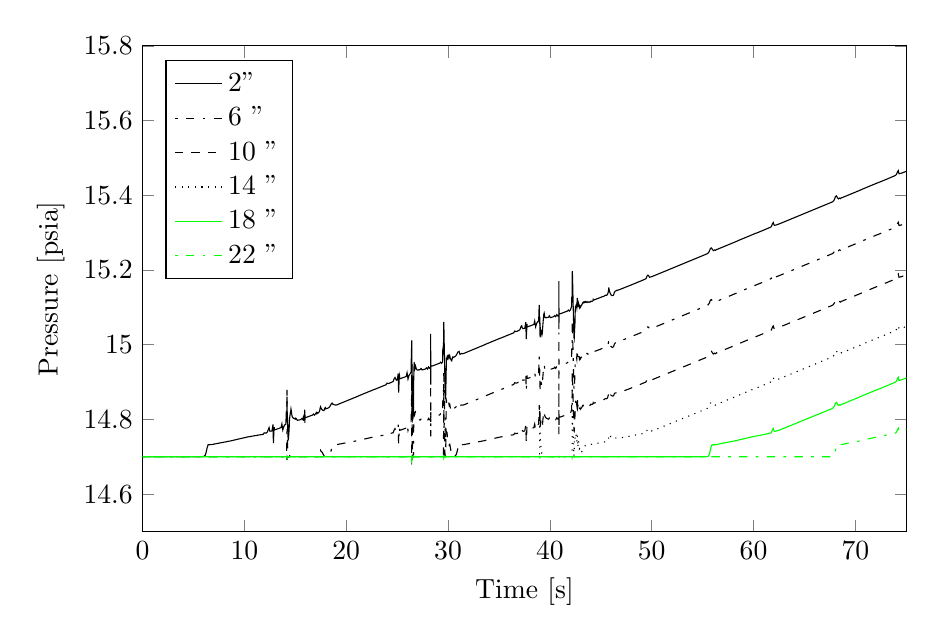
\begin{tikzpicture}

\begin{axis}[%
width=0.8\textwidth,
height=0.508815326102268\textwidth,
scale only axis,
xmin=0.0,
xmax=75.0,
xlabel={Time [s]},
ymin=14.5,
ymax=15.8,
ylabel={Pressure [psia]},
legend style={at={(0.03,0.97)},anchor=north west,draw=black,fill=white,legend cell align=left}
]
\addplot [
color=black,
solid
]
table[row sep=crcr]{
0 14.7007818222046\\
9.99999971718069e-10 14.7007818222046\\
2.49999998480632e-09 14.7007818222046\\
4.74999994892755e-09 14.7007818222046\\
8.1250002281763e-09 14.7007818222046\\
1.31874999809156e-08 14.7007818222046\\
2.0781250498203e-08 14.7007818222046\\
3.21718758300449e-08 14.7007818222046\\
4.92578138278077e-08 14.7007818222046\\
7.48867208244519e-08 14.7007818222046\\
1.13330081319418e-07 14.7007818222046\\
1.70995122061868e-07 14.7007818222046\\
2.57492672517401e-07 14.7007818222046\\
3.8723902662241e-07 14.7007818222046\\
5.81858500936505e-07 14.7007818222046\\
8.73787769251066e-07 14.7007818222046\\
1.31168167172291e-06 14.7007818222046\\
1.9685226106958e-06 14.7007827758789\\
2.95378367809462e-06 14.7007827758789\\
4.43167573394021e-06 14.7007827758789\\
6.64851359033491e-06 14.7007827758789\\
9.97376992017962e-06 14.7007837295532\\
1.49616553244414e-05 14.7007846832275\\
2.24434825213393e-05 14.7007856369019\\
3.36662233166862e-05 14.7007865905762\\
5.05003372381907e-05 14.7007884979248\\
7.57515081204474e-05 14.7007904052734\\
0.000113628258986864 14.7007932662964\\
0.000170443381648511 14.700795173645\\
0.000255666091106832 14.7007970809937\\
0.000383500126190484 14.7007970809937\\
0.000575251178815961 14.7007942199707\\
0.000862877757754177 14.7007904052734\\
0.00129431765526533 14.7007865905762\\
0.00194147753063589 14.7007837295532\\
0.00291221728548408 14.700779914856\\
0.00436832662671804 14.7007780075073\\
0.00597004732117057 14.700779914856\\
0.00773194013163447 14.7007827758789\\
0.009670021943748 14.7007837295532\\
0.0118019115179777 14.7007837295532\\
0.0141469910740852 14.7007827758789\\
0.0167265776544809 14.7007827758789\\
0.0195641238242388 14.7007827758789\\
0.0226854234933853 14.7007827758789\\
0.0261188540607691 14.7007827758789\\
0.0298956278711557 14.7007827758789\\
0.0340500771999359 14.7007827758789\\
0.0386199727654457 14.7007827758789\\
0.0436468608677387 14.7007827758789\\
0.0491764321923256 14.7007827758789\\
0.0552589632570744 14.7007827758789\\
0.0619497485458851 14.7007827758789\\
0.0693096145987511 14.7007827758789\\
0.0774054601788521 14.7007827758789\\
0.0863108932971954 14.700779914856\\
0.0961068719625473 14.7007827758789\\
0.106882445514202 14.7007827758789\\
0.118735581636429 14.7007827758789\\
0.13177402317524 14.7007827758789\\
0.146116316318512 14.7007827758789\\
0.161892831325531 14.7007827758789\\
0.179247006773949 14.7007827758789\\
0.198336601257324 14.7007827758789\\
0.21933513879776 14.7007827758789\\
0.242433547973633 14.7007827758789\\
0.267841786146164 14.7007827758789\\
0.29579085111618 14.7007827758789\\
0.32653483748436 14.7007827758789\\
0.360353201627731 14.7007827758789\\
0.397553414106369 14.7007837295532\\
0.438473641872406 14.7007837295532\\
0.483485877513886 14.7007837295532\\
0.532999336719513 14.7007837295532\\
0.587464153766632 14.7007837295532\\
0.647375464439392 14.7007837295532\\
0.71327793598175 14.7007837295532\\
0.7857705950737 14.7007837295532\\
0.865512549877167 14.7007837295532\\
0.953228712081909 14.7007837295532\\
1.04971647262573 14.7007837295532\\
1.14971649646759 14.7007827758789\\
1.24971640110016 14.7007827758789\\
1.34971642494202 14.7007827758789\\
1.44971644878387 14.7007827758789\\
1.54971647262573 14.7007827758789\\
1.64971649646759 14.7007827758789\\
1.74971640110016 14.7007827758789\\
1.84971642494202 14.7007827758789\\
1.94971644878387 14.7007827758789\\
2.04971647262573 14.7007827758789\\
2.1497163772583 14.7007827758789\\
2.24971652030945 14.7007827758789\\
2.34971642494202 14.7007827758789\\
2.44971656799316 14.7007827758789\\
2.54971647262573 14.7007827758789\\
2.6497163772583 14.7007827758789\\
2.74971652030945 14.7007827758789\\
2.84971642494202 14.7007827758789\\
2.94971656799316 14.7007827758789\\
3.04971647262573 14.7007827758789\\
3.1497163772583 14.7007827758789\\
3.24971652030945 14.7007827758789\\
3.34971642494202 14.7007827758789\\
3.44971656799316 14.7007827758789\\
3.54971647262573 14.7007827758789\\
3.6497163772583 14.7007827758789\\
3.74971652030945 14.7007827758789\\
3.84971642494202 14.7007827758789\\
3.94971656799316 14.7007827758789\\
4.04971647262573 14.7007827758789\\
4.1497163772583 14.7007827758789\\
4.24971628189087 14.7007827758789\\
4.3497166633606 14.7007827758789\\
4.44971656799316 14.7007827758789\\
4.54971647262573 14.7007827758789\\
4.6497163772583 14.7007827758789\\
4.74971628189087 14.7007827758789\\
4.8497166633606 14.7007827758789\\
4.94971656799316 14.7007827758789\\
5.04971647262573 14.7007837295532\\
5.1497163772583 14.7007837295532\\
5.24971628189087 14.7007837295532\\
5.3497166633606 14.7007837295532\\
5.44971656799316 14.7007837295532\\
5.54971647262573 14.7007837295532\\
5.6497163772583 14.7007837295532\\
5.74971628189087 14.7007884979248\\
5.8497166633606 14.7008085250854\\
5.94971656799316 14.70090675354\\
6.04971647262573 14.7014398574829\\
6.1497163772583 14.704080581665\\
6.24971628189087 14.7125511169434\\
6.3497166633606 14.725396156311\\
6.44971656799316 14.7330207824707\\
6.54971647262573 14.732325553894\\
6.6497163772583 14.733006477356\\
6.74971628189087 14.732626914978\\
6.8497166633606 14.7333736419678\\
6.94971656799316 14.7336568832397\\
7.04971647262573 14.734393119812\\
7.1497163772583 14.7347822189331\\
7.24971628189087 14.7354030609131\\
7.3497166633606 14.7358684539795\\
7.44971656799316 14.7364387512207\\
7.54971647262573 14.7369375228882\\
7.6497163772583 14.7374849319458\\
7.74971628189087 14.7379999160767\\
7.8497166633606 14.7385368347168\\
7.94971656799316 14.7390584945679\\
8.04971599578857 14.7395906448364\\
8.1497163772583 14.7401151657104\\
8.24971675872803 14.7406454086304\\
8.34971618652344 14.741171836853\\
8.44971656799316 14.7417011260986\\
8.54971599578857 14.7422285079956\\
8.6497163772583 14.7427568435669\\
8.74971675872803 14.7432851791382\\
8.84971618652344 14.743842124939\\
8.94971656799316 14.744704246521\\
9.04971599578857 14.7452869415283\\
9.1497163772583 14.7459402084351\\
9.24971675872803 14.7465677261353\\
9.34971618652344 14.7472019195557\\
9.44971656799316 14.7478313446045\\
9.54971599578857 14.748459815979\\
9.6497163772583 14.7490863800049\\
9.74971675872803 14.7497119903564\\
9.84971618652344 14.7503356933594\\
9.94971656799316 14.750958442688\\
10.0497159957886 14.751579284668\\
10.1497163772583 14.7521991729736\\
10.249716758728 14.752818107605\\
10.3497161865234 14.7534303665161\\
10.4497165679932 14.7537994384766\\
10.5497159957886 14.7542762756348\\
10.6497163772583 14.7548017501831\\
10.749716758728 14.7553043365479\\
10.8497161865234 14.7558059692383\\
10.9497165679932 14.7562980651855\\
11.0497159957886 14.7567825317383\\
11.1497163772583 14.7572574615479\\
11.249716758728 14.7577199935913\\
11.3497161865234 14.7581701278687\\
11.4497165679932 14.7586069107056\\
11.5497159957886 14.7590341567993\\
11.6497163772583 14.7594566345215\\
11.749716758728 14.7598266601563\\
11.8497161865234 14.7601566314697\\
11.9497165679932 14.7643003463745\\
12.0497159957886 14.7638158798218\\
12.1497163772583 14.7637815475464\\
12.249716758728 14.7665519714355\\
12.347146987915 14.7727012634277\\
12.4250946044922 14.7783174514771\\
12.4874591827393 14.7692184448242\\
12.5560598373413 14.7686729431152\\
12.6315202713013 14.7690563201904\\
12.714527130127 14.7695341110229\\
12.8058338165283 14.7866821289063\\
12.8497476577759 14.7367706298828\\
12.8980522155762 14.7679605484009\\
12.9143037796021 14.7766189575195\\
12.9277105331421 14.7797164916992\\
12.9424571990967 14.7722702026367\\
12.9586782455444 14.7723064422607\\
12.9765224456787 14.772406578064\\
12.9961500167847 14.7725305557251\\
13.0177412033081 14.77268409729\\
13.0414915084839 14.7728700637817\\
13.0676164627075 14.7730894088745\\
13.0963535308838 14.7733449935913\\
13.1279649734497 14.7736377716064\\
13.1627368927002 14.7739715576172\\
13.2009868621826 14.7743463516235\\
13.2430610656738 14.7747659683228\\
13.289342880249 14.7752323150635\\
13.3402528762817 14.7757482528687\\
13.3962545394897 14.7763185501099\\
13.4578561782837 14.7769460678101\\
13.5256175994873 14.7776365280151\\
13.600154876709 14.778395652771\\
13.6821460723877 14.7879543304443\\
13.7723369598389 14.7718334197998\\
13.871545791626 14.7812509536743\\
13.9715461730957 14.7859354019165\\
14.0715456008911 14.7874317169189\\
14.1215467453003 14.8222885131836\\
14.147439956665 14.8224458694458\\
14.1759233474731 14.8214206695557\\
14.1775197982788 14.8230495452881\\
14.1792755126953 14.8388214111328\\
14.1812076568604 14.8541812896729\\
14.1833324432373 14.8612461090088\\
14.1856698989868 14.8579320907593\\
14.1882400512695 14.848048210144\\
14.191068649292 14.8357906341553\\
14.1941795349121 14.8241014480591\\
14.1976013183594 14.8225889205933\\
14.2013654708862 14.8215818405151\\
14.2055063247681 14.8197231292725\\
14.2100610733032 14.8171873092651\\
14.2150716781616 14.8140468597412\\
14.2205829620361 14.81028175354\\
14.2266454696655 14.8058986663818\\
14.2333135604858 14.8009548187256\\
14.2406492233276 14.7955570220947\\
14.2487182617188 14.7895851135254\\
14.2575941085815 14.7806301116943\\
14.2673578262329 14.7690601348877\\
14.27809715271 14.7588787078857\\
14.2899112701416 14.7508697509766\\
14.3029069900513 14.7460966110229\\
14.3172016143799 14.7458801269531\\
14.3329257965088 14.7500343322754\\
14.3502225875854 14.7575302124023\\
14.3692483901978 14.764627456665\\
14.3901777267456 14.7696876525879\\
14.4131994247437 14.7905673980713\\
14.4385232925415 14.8013181686401\\
14.4663791656494 14.8087797164917\\
14.4970216751099 14.8139886856079\\
14.520975112915 14.8184442520142\\
14.5473232269287 14.8209476470947\\
14.5763063430786 14.8280334472656\\
14.6081876754761 14.8234481811523\\
14.6432571411133 14.8154821395874\\
14.6818342208862 14.8090295791626\\
14.7242679595947 14.8064222335815\\
14.7709455490112 14.8045387268066\\
14.8222913742065 14.8033390045166\\
14.8712491989136 14.8034515380859\\
14.9185028076172 14.8024024963379\\
14.9638071060181 14.8014860153198\\
15.0066013336182 14.8008108139038\\
15.0464649200439 14.8033781051636\\
15.0903158187866 14.8021049499512\\
15.1385507583618 14.8002147674561\\
15.1916093826294 14.7980537414551\\
15.2499742507935 14.7981424331665\\
15.3141756057739 14.7984142303467\\
15.3847970962524 14.7987470626831\\
15.4624805450439 14.7992877960205\\
15.5479326248169 14.7999620437622\\
15.6419296264648 14.8027620315552\\
15.7419300079346 14.7995977401733\\
15.7919301986694 14.8068828582764\\
15.8469295501709 14.7996120452881\\
15.9074296951294 14.8025875091553\\
15.920783996582 14.8267011642456\\
15.9354724884033 14.7910566329956\\
15.9516305923462 14.8026876449585\\
15.9645795822144 14.8078603744507\\
15.9788236618042 14.8051252365112\\
15.9944925308228 14.8051795959473\\
16.0117282867432 14.8052787780762\\
16.0306873321533 14.8054027557373\\
16.0515422821045 14.8055582046509\\
16.0744819641113 14.8057441711426\\
16.0997161865234 14.8059644699097\\
16.1274738311768 14.8062191009521\\
16.1580085754395 14.8065099716187\\
16.1915950775146 14.8068380355835\\
16.2285404205322 14.8072052001953\\
16.2691822052002 14.8076133728027\\
16.3138847351074 14.8080654144287\\
16.3630599975586 14.8085641860962\\
16.4171524047852 14.8091144561768\\
16.4766540527344 14.8097200393677\\
16.542106628418 14.8103857040405\\
16.6141033172607 14.8111190795898\\
16.6932983398438 14.8119249343872\\
16.7804145812988 14.8146600723267\\
16.87624168396 14.8118324279785\\
16.9762420654297 14.8149604797363\\
17.0762424468994 14.8186702728271\\
17.0962505340576 14.8169832229614\\
17.1021957397461 14.8160438537598\\
17.1087341308594 14.8157091140747\\
17.1159267425537 14.8163604736328\\
17.1238384246826 14.8173379898071\\
17.1325416564941 14.8179922103882\\
17.1421165466309 14.8181858062744\\
17.1526470184326 14.8177623748779\\
17.1642322540283 14.8177585601807\\
17.1769752502441 14.8181552886963\\
17.1909923553467 14.8182220458984\\
17.2064094543457 14.8181581497192\\
17.2233715057373 14.8179349899292\\
17.2420272827148 14.8172750473022\\
17.2625503540039 14.817795753479\\
17.2851238250732 14.8186664581299\\
17.3099555969238 14.8194894790649\\
17.3372707366943 14.8202610015869\\
17.367317199707 14.8214244842529\\
17.400369644165 14.824499130249\\
17.4367256164551 14.8309907913208\\
17.4767169952393 14.8342952728271\\
17.5207099914551 14.8310642242432\\
17.5690994262695 14.8282308578491\\
17.6223297119141 14.8265428543091\\
17.6808815002441 14.8251361846924\\
17.745288848877 14.8237962722778\\
17.8161373138428 14.8237657546997\\
17.8624935150146 14.8278837203979\\
17.9028415679932 14.8306369781494\\
17.9472217559814 14.8317584991455\\
17.9960422515869 14.8284797668457\\
18.0497417449951 14.8292589187622\\
18.108814239502 14.8296241760254\\
18.173791885376 14.8301248550415\\
18.245267868042 14.8310031890869\\
18.3238925933838 14.8325843811035\\
18.41037940979 14.8356885910034\\
18.5055141448975 14.8405809402466\\
18.6055145263672 14.8439178466797\\
18.7055149078369 14.8405122756958\\
18.805513381958 14.8397369384766\\
18.9055137634277 14.8389377593994\\
19.0055141448975 14.8386125564575\\
19.1055145263672 14.8394756317139\\
19.2055149078369 14.8405332565308\\
19.305513381958 14.8418436050415\\
19.4055137634277 14.8428249359131\\
19.5055141448975 14.8440217971802\\
19.6055145263672 14.8450775146484\\
19.7055149078369 14.846227645874\\
19.805513381958 14.8473148345947\\
19.9055137634277 14.8484697341919\\
20.0055141448975 14.8495569229126\\
20.1055145263672 14.8506593704224\\
20.2055149078369 14.8517713546753\\
20.305513381958 14.8528823852539\\
20.4055137634277 14.8539962768555\\
20.5055141448975 14.8551092147827\\
20.6055145263672 14.8562231063843\\
20.7055149078369 14.8573360443115\\
20.805513381958 14.8584508895874\\
20.9055137634277 14.859564781189\\
21.0055141448975 14.8606786727905\\
21.1055145263672 14.8617935180664\\
21.2055149078369 14.862982749939\\
21.305513381958 14.8643550872803\\
21.4055137634277 14.8654136657715\\
21.5055141448975 14.8665447235107\\
21.6055145263672 14.867657661438\\
21.7055149078369 14.8687791824341\\
21.805513381958 14.8698987960815\\
21.9055137634277 14.871018409729\\
22.0055141448975 14.8721380233765\\
22.1055145263672 14.8732585906982\\
22.2055149078369 14.87437915802\\
22.305513381958 14.8754987716675\\
22.4055137634277 14.8766193389893\\
22.5055141448975 14.8777408599854\\
22.6055145263672 14.8788614273071\\
22.7055149078369 14.8799819946289\\
22.805513381958 14.8809013366699\\
22.9055137634277 14.8819103240967\\
23.0055141448975 14.8830518722534\\
23.1055145263672 14.8841466903687\\
23.2055149078369 14.8852558135986\\
23.305513381958 14.8863582611084\\
23.4055137634277 14.8874597549438\\
23.5055141448975 14.888557434082\\
23.6055145263672 14.8896532058716\\
23.7055149078369 14.8907442092896\\
23.805513381958 14.8918313980103\\
23.9055137634277 14.8929147720337\\
24.0055141448975 14.8973426818848\\
24.1055145263672 14.8963432312012\\
24.2055149078369 14.8965749740601\\
24.305513381958 14.897912979126\\
24.4055137634277 14.899019241333\\
24.5055141448975 14.9002637863159\\
24.6055145263672 14.9015207290649\\
24.7055149078369 14.9091014862061\\
24.789867401123 14.9124031066895\\
24.8573379516602 14.908429145813\\
24.9315567016602 14.9052228927612\\
25.0131969451904 14.9058017730713\\
25.1030006408691 14.9229736328125\\
25.1443557739258 14.8719282150269\\
25.189847946167 14.9017992019653\\
25.2099170684814 14.9156122207642\\
25.2266445159912 14.9176540374756\\
25.245044708252 14.9090824127197\\
25.2652854919434 14.9091358184814\\
25.2875499725342 14.9092798233032\\
25.3120403289795 14.9094495773315\\
25.3389797210693 14.9096584320068\\
25.3686122894287 14.9099073410034\\
25.4012107849121 14.9101982116699\\
25.4370670318604 14.9105339050293\\
25.4765090942383 14.9109153747559\\
25.5198955535889 14.9113464355469\\
25.5676212310791 14.911828994751\\
25.6201171875 14.9123640060425\\
25.6778659820557 14.9129552841187\\
25.7413883209229 14.9136066436768\\
25.8112621307373 14.9143228530884\\
25.8881244659424 14.9151105880737\\
25.9726715087891 14.9250268936157\\
26.065673828125 14.9084243774414\\
26.1656742095947 14.9180812835693\\
26.2656745910645 14.9219942092896\\
26.3656749725342 14.9271039962769\\
26.409065246582 14.9905433654785\\
26.4240894317627 14.9428100585938\\
26.4268970489502 14.9467554092407\\
26.4299831390381 14.9844131469727\\
26.4333801269531 15.0116138458252\\
26.4371166229248 15.006160736084\\
26.4412250518799 14.9833459854126\\
26.4457454681396 14.9567747116089\\
26.4507179260254 14.9507646560669\\
26.4561862945557 14.9450531005859\\
26.4622020721436 14.9374942779541\\
26.4688205718994 14.9286851882935\\
26.4761009216309 14.9186964035034\\
26.4841079711914 14.9024829864502\\
26.4929161071777 14.8745708465576\\
26.5026054382324 14.8438882827759\\
26.5132637023926 14.8130626678467\\
26.5249881744385 14.8001461029053\\
26.5378837585449 14.8013877868652\\
26.5520706176758 14.8034315109253\\
26.5676746368408 14.8064813613892\\
26.5848388671875 14.8114957809448\\
26.6037216186523 14.823561668396\\
26.624490737915 14.9041938781738\\
26.6473369598389 14.9308948516846\\
26.6724681854248 14.9534959793091\\
26.7001132965088 14.9321537017822\\
26.7305221557617 14.934362411499\\
26.7594413757324 14.9430532455444\\
26.7881412506104 14.9447593688965\\
26.8180274963379 14.9418487548828\\
26.848762512207 14.9389333724976\\
26.8805618286133 14.9358825683594\\
26.9128971099854 14.9342393875122\\
26.9456844329834 14.9331693649292\\
26.97873878479 14.9324254989624\\
27.0120601654053 14.9320163726807\\
27.0457935333252 14.9321355819702\\
27.0821418762207 14.932279586792\\
27.1221237182617 14.9328956604004\\
27.1524639129639 14.9334154129028\\
27.1838111877441 14.9332399368286\\
27.2182941436768 14.9331483840942\\
27.2558403015137 14.9333639144897\\
27.2955665588379 14.9349718093872\\
27.3392658233643 14.9365282058716\\
27.3873329162598 14.9355592727661\\
27.4402103424072 14.932731628418\\
27.4983730316162 14.9329652786255\\
27.5623531341553 14.9334697723389\\
27.6327304840088 14.9339361190796\\
27.7101459503174 14.9345626831055\\
27.7953014373779 14.935338973999\\
27.8889751434326 14.9383172988892\\
27.9889755249023 14.935079574585\\
28.0889739990234 14.9406566619873\\
28.1889743804932 14.9370632171631\\
28.2889747619629 14.9397621154785\\
28.2927665710449 15.029182434082\\
28.2969398498535 14.8933029174805\\
28.3015289306641 14.9227323532104\\
28.304780960083 14.9578008651733\\
28.307991027832 14.9553022384644\\
28.3115215301514 14.9428262710571\\
28.3154048919678 14.9426984786987\\
28.3196773529053 14.9427585601807\\
28.3243770599365 14.942756652832\\
28.3295459747314 14.9427576065063\\
28.3352317810059 14.9427623748779\\
28.3414859771729 14.9427719116211\\
28.3483657836914 14.9427871704102\\
28.3559341430664 14.9428091049194\\
28.3642578125 14.9428386688232\\
28.3734169006348 14.9428787231445\\
28.3834896087646 14.9429292678833\\
28.3945693969727 14.9429922103882\\
28.4067573547363 14.9430694580078\\
28.4201641082764 14.9431619644165\\
28.4349136352539 14.9432725906372\\
28.451135635376 14.9434022903442\\
28.4689807891846 14.9435529708862\\
28.4886093139648 14.9437265396118\\
28.5102024078369 14.9439249038696\\
28.5339546203613 14.9441499710083\\
28.5600814819336 14.9444036483765\\
28.5888214111328 14.9446878433228\\
28.620433807373 14.9450044631958\\
28.6552085876465 14.9453554153442\\
28.6934604644775 14.9457445144653\\
28.735538482666 14.946174621582\\
28.7818241119385 14.9466485977173\\
28.8327369689941 14.9471702575684\\
28.8887424468994 14.9477443695068\\
28.9503479003906 14.9483757019043\\
29.0181159973145 14.949070930481\\
29.092658996582 14.9498357772827\\
29.1746559143066 14.9506769180298\\
29.2648525238037 14.9534139633179\\
29.3640689849854 14.9506978988647\\
29.4640693664551 14.9538469314575\\
29.4847068786621 14.990306854248\\
29.4888343811035 14.9767799377441\\
29.4933738708496 14.9730243682861\\
29.4983692169189 14.9749917984009\\
29.5038623809814 14.9799671173096\\
29.5099067687988 14.9851007461548\\
29.5165538787842 14.9893236160278\\
29.5230560302734 14.9923229217529\\
29.5302066802979 14.992057800293\\
29.5380744934082 14.9914808273315\\
29.5467281341553 14.9924287796021\\
29.556245803833 15.0068359375\\
29.5667171478271 15.0434789657593\\
29.5782356262207 15.0608205795288\\
29.5909042358398 15.048900604248\\
29.6048412322998 15.0223159790039\\
29.6201705932617 15.0033016204834\\
29.637035369873 14.98193359375\\
29.6555843353271 14.9575176239014\\
29.675989151001 14.9270372390747\\
29.6984329223633 14.8900175094604\\
29.7114696502686 14.8749370574951\\
29.7258071899414 14.865478515625\\
29.7415809631348 14.8589191436768\\
29.7589302062988 14.8572874069214\\
29.7780151367188 14.8754825592041\\
29.7990093231201 14.9062395095825\\
29.8221015930176 14.9403438568115\\
29.8475036621094 14.9625034332275\\
29.8754444122314 14.9619789123535\\
29.9061813354492 14.9667282104492\\
29.9399909973145 14.9624214172363\\
29.9771823883057 14.9616079330444\\
30.0180931091309 14.9706830978394\\
30.0630931854248 14.9721250534058\\
30.1125946044922 14.9658699035645\\
30.1670475006104 14.9701681137085\\
30.2269439697266 14.9626846313477\\
30.2706527709961 14.9616565704346\\
30.318733215332 14.9579372406006\\
30.3593273162842 14.9569540023804\\
30.3947944641113 14.9615793228149\\
30.4330863952637 14.9652519226074\\
30.4652576446533 14.9671697616577\\
30.5006484985352 14.9657430648804\\
30.5330505371094 14.9660358428955\\
30.5677318572998 14.9668111801147\\
30.6004276275635 14.967357635498\\
30.6349658966064 14.9677438735962\\
30.6682662963867 14.9683675765991\\
30.7048969268799 14.9690294265747\\
30.7451915740967 14.9700117111206\\
30.789514541626 14.9714412689209\\
30.8382682800293 14.9735927581787\\
30.8918991088867 14.9766263961792\\
30.9508934020996 14.9801692962646\\
31.0157871246338 14.9810523986816\\
31.0871696472168 14.9822988510132\\
31.1656913757324 14.9743814468384\\
31.2520637512207 14.9756555557251\\
31.347074508667 14.9767618179321\\
31.4470748901367 14.976035118103\\
31.5470752716064 14.9768695831299\\
31.6470737457275 14.9779739379883\\
31.7470741271973 14.9792556762695\\
31.847074508667 14.9802827835083\\
31.9470748901367 14.9814729690552\\
32.0470733642578 14.9825601577759\\
32.1470756530762 14.9837141036987\\
32.2470741271973 14.984842300415\\
32.3470764160156 14.9859609603882\\
32.4470748901367 14.9870824813843\\
32.5470733642578 14.9882154464722\\
32.6470756530762 14.9893407821655\\
32.7470741271973 14.9904708862305\\
32.8470764160156 14.9915981292725\\
32.9470748901367 14.9927272796631\\
33.0470733642578 14.9938554763794\\
33.1470756530762 14.99498462677\\
33.2470741271973 14.9961128234863\\
33.3470764160156 14.9972410202026\\
33.4470748901367 14.9983692169189\\
33.5470733642578 14.9994983673096\\
33.6470756530762 15.0007028579712\\
33.7470741271973 15.0020895004272\\
33.8470764160156 15.0031490325928\\
33.9470748901367 15.0042991638184\\
34.0470733642578 15.0054216384888\\
34.1470756530762 15.0065517425537\\
34.2470741271973 15.0076808929443\\
34.3470764160156 15.0088090896606\\
34.4470748901367 15.0099382400513\\
34.5470733642578 15.0110673904419\\
34.6470756530762 15.0121955871582\\
34.7470741271973 15.0133247375488\\
34.8470764160156 15.0144529342651\\
34.9470748901367 15.0155820846558\\
35.0470733642578 15.0167102813721\\
35.1470756530762 15.0178375244141\\
35.2470741271973 15.0187406539917\\
35.3470764160156 15.0197877883911\\
35.4470748901367 15.0209245681763\\
35.5470733642578 15.0220308303833\\
35.6470756530762 15.0231447219849\\
35.7470741271973 15.0242538452148\\
35.8470764160156 15.0253620147705\\
35.9470748901367 15.0264663696289\\
36.0470733642578 15.02756690979\\
36.1470756530762 15.0286645889282\\
36.2470741271973 15.0297565460205\\
36.3470764160156 15.0308456420898\\
36.4470748901367 15.0319299697876\\
36.5470733642578 15.0367088317871\\
36.6470756530762 15.0355014801025\\
36.7470741271973 15.0357141494751\\
36.8470764160156 15.0370750427246\\
36.9470748901367 15.0382385253906\\
37.0470733642578 15.0399618148804\\
37.1470756530762 15.0478219985962\\
37.2293395996094 15.0507116317749\\
37.2951393127441 15.0446720123291\\
37.3675231933594 15.0430946350098\\
37.4471435546875 15.0437049865723\\
37.534725189209 15.0443515777588\\
37.6310653686523 15.0602254867554\\
37.6772041320801 15.0154504776001\\
37.7279586791992 15.0434455871582\\
37.7453880310059 15.0559968948364\\
37.7602653503418 15.0504083633423\\
37.7766304016113 15.0480985641479\\
37.7946319580078 15.0481758117676\\
37.8144378662109 15.0482902526855\\
37.8362197875977 15.0484342575073\\
37.860179901123 15.0486125946045\\
37.8865356445313 15.048828125\\
37.9155311584473 15.0490818023682\\
37.9474220275879 15.0493755340576\\
37.9825019836426 15.0497102737427\\
38.0210914611816 15.0500898361206\\
38.0635414123535 15.0505151748657\\
38.1102333068848 15.050989151001\\
38.1615982055664 15.051513671875\\
38.2180976867676 15.0520925521851\\
38.2802429199219 15.0527305603027\\
38.3486099243164 15.0534334182739\\
38.4238090515137 15.0542049407959\\
38.5065269470215 15.0635442733765\\
38.5975189208984 15.0479984283447\\
38.6975212097168 15.0571489334106\\
38.7975196838379 15.0615015029907\\
38.8975219726563 15.0646104812622\\
38.9475212097168 15.1068248748779\\
38.9856338500977 15.0554523468018\\
39.0002326965332 15.0596685409546\\
39.0162887573242 15.074875831604\\
39.0339508056641 15.0196542739868\\
39.0533828735352 15.0236587524414\\
39.0747528076172 15.0281391143799\\
39.0982627868652 15.0386371612549\\
39.1241226196289 15.0343189239502\\
39.1525688171387 15.0356178283691\\
39.1838569641113 15.0318927764893\\
39.2182769775391 15.0263814926147\\
39.2382202148438 15.0288171768188\\
39.2601547241211 15.0320692062378\\
39.2842864990234 15.0438995361328\\
39.3108291625977 15.0539636611938\\
39.3400230407715 15.0636329650879\\
39.3721389770508 15.071759223938\\
39.4047470092773 15.0824699401855\\
39.4365348815918 15.0848035812378\\
39.4690742492676 15.0786380767822\\
39.5013847351074 15.073860168457\\
39.5341873168945 15.0730228424072\\
39.5668563842773 15.0727167129517\\
39.5998191833496 15.0723686218262\\
39.632698059082 15.0722303390503\\
39.6657829284668 15.0726518630981\\
39.6988639831543 15.0733270645142\\
39.7321624755859 15.0734090805054\\
39.7687873840332 15.0733156204224\\
39.8090744018555 15.0733938217163\\
39.8533935546875 15.0735673904419\\
39.8968162536621 15.0747079849243\\
39.939453125 15.0775203704834\\
39.9863548278809 15.0754022598267\\
40.0379447937012 15.0727977752686\\
40.0946960449219 15.0729818344116\\
40.1571197509766 15.0735454559326\\
40.2257843017578 15.0739345550537\\
40.3013191223145 15.0745630264282\\
40.384407043457 15.0753135681152\\
40.4758033752441 15.0781593322754\\
40.5758018493652 15.0751533508301\\
40.6758041381836 15.0804147720337\\
40.7758026123047 15.0771484375\\
40.875804901123 15.0795545578003\\
40.8792419433594 15.1705026626587\\
40.8830223083496 15.0418367385864\\
40.8871841430664 15.0566053390503\\
40.8903007507324 15.0976390838623\\
40.8937301635742 15.0959091186523\\
40.8975028991699 15.0830898284912\\
40.9016532897949 15.0823287963867\\
40.9062156677246 15.0826759338379\\
40.9112396240234 15.0827026367188\\
40.9167633056641 15.0826959609985\\
40.9228363037109 15.0826978683472\\
40.9295196533203 15.082706451416\\
40.9368743896484 15.0827217102051\\
40.9449615478516 15.0827445983887\\
40.953857421875 15.0827770233154\\
40.9636421203613 15.0828189849854\\
40.9744033813477 15.0828733444214\\
40.9862442016602 15.0829420089722\\
40.999267578125 15.083025932312\\
41.0135955810547 15.0831279754639\\
41.029354095459 15.0832481384277\\
41.046688079834 15.0833892822266\\
41.0657577514648 15.083553314209\\
41.0867347717285 15.0837421417236\\
41.109806060791 15.0839576721191\\
41.1351852416992 15.0842008590698\\
41.1631050109863 15.0844745635986\\
41.1938133239746 15.0847806930542\\
41.227596282959 15.0851202011108\\
41.2647552490234 15.0854978561401\\
41.3056297302246 15.0859146118164\\
41.3505935668945 15.0863742828369\\
41.4000511169434 15.0868816375732\\
41.4544563293457 15.087438583374\\
41.5143013000488 15.0880527496338\\
41.5801315307617 15.0887279510498\\
41.6525421142578 15.0894708633423\\
41.7321968078613 15.0902881622314\\
41.8198165893555 15.0929698944092\\
41.9161987304688 15.0902862548828\\
42.0161972045898 15.0933780670166\\
42.1161994934082 15.1014089584351\\
42.1361999511719 15.1044054031372\\
42.1442070007324 15.1263380050659\\
42.1520309448242 15.1286678314209\\
42.1606330871582 15.1251840591431\\
42.1689529418945 15.1250610351563\\
42.1781005859375 15.1263246536255\\
42.1881637573242 15.1490697860718\\
42.1992378234863 15.196873664856\\
42.2114143371582 15.189733505249\\
42.2248077392578 15.1753234863281\\
42.2395439147949 15.1590957641602\\
42.2557525634766 15.1399297714233\\
42.2735824584961 15.1175594329834\\
42.2931938171387 15.0951271057129\\
42.3147659301758 15.0735559463501\\
42.3384971618652 15.0424995422363\\
42.3646011352539 15.0191345214844\\
42.3847808837891 15.0164680480957\\
42.4069786071777 15.0296792984009\\
42.431396484375 15.0430812835693\\
42.4582557678223 15.0570974349976\\
42.4878005981445 15.0924634933472\\
42.5203018188477 15.102765083313\\
42.5560493469238 15.104564666748\\
42.5953750610352 15.1070861816406\\
42.6386299133301 15.1000471115112\\
42.6862144470215 15.1255187988281\\
42.7385559082031 15.1007146835327\\
42.7959022521973 15.1126689910889\\
42.8589859008789 15.1065330505371\\
42.9028167724609 15.099627494812\\
42.9510307312012 15.1031665802002\\
42.9925117492676 15.1003246307373\\
43.0297622680664 15.1022920608521\\
43.0707359313965 15.1042146682739\\
43.1158065795898 15.1059608459473\\
43.1579742431641 15.108437538147\\
43.203685760498 15.1111583709717\\
43.2497863769531 15.1133432388306\\
43.3005027770996 15.112265586853\\
43.3562850952148 15.1151332855225\\
43.4176483154297 15.1133279800415\\
43.4851493835449 15.115701675415\\
43.559398651123 15.1133918762207\\
43.6410713195801 15.1153106689453\\
43.7309150695801 15.1132593154907\\
43.8297386169434 15.1149082183838\\
43.9297409057617 15.1136474609375\\
44.0297393798828 15.1167106628418\\
44.1297416687012 15.1160287857056\\
44.2297401428223 15.1178121566772\\
44.2499618530273 15.1207723617554\\
44.2722015380859 15.1194009780884\\
44.2966690063477 15.1196460723877\\
44.3235816955566 15.1199216842651\\
44.3531875610352 15.1202249526978\\
44.3857498168945 15.1205577850342\\
44.421573638916 15.120924949646\\
44.4609756469727 15.1213293075562\\
44.5043182373047 15.1217737197876\\
44.5519981384277 15.1222620010376\\
44.6044425964355 15.1227998733521\\
44.6621360778809 15.1233921051025\\
44.7255935668945 15.1240425109863\\
44.7953987121582 15.1247587203979\\
44.872184753418 15.1255464553833\\
44.9566497802734 15.1264123916626\\
45.0495643615723 15.127366065979\\
45.1495628356934 15.1290063858032\\
45.2495613098145 15.1289091110229\\
45.3495635986328 15.1305780410767\\
45.4495620727539 15.1325855255127\\
45.5495643615723 15.1322498321533\\
45.6495628356934 15.1340141296387\\
45.7495613098145 15.143045425415\\
45.7695655822754 15.1518993377686\\
45.7816352844238 15.1519794464111\\
45.7949142456055 15.1501445770264\\
45.8095207214355 15.1481800079346\\
45.8255882263184 15.1468181610107\\
45.8432655334473 15.145131111145\\
45.8627052307129 15.1430063247681\\
45.884090423584 15.1402645111084\\
45.9076156616211 15.1387748718262\\
45.9334945678711 15.137110710144\\
45.9619598388672 15.1353178024292\\
45.9932708740234 15.1338310241699\\
46.0277099609375 15.1329689025879\\
46.0655975341797 15.1322021484375\\
46.1072731018066 15.1316795349121\\
46.1531181335449 15.131516456604\\
46.2035446166992 15.1321287155151\\
46.2590141296387 15.1336517333984\\
46.3200302124023 15.1395454406738\\
46.387149810791 15.1426134109497\\
46.4504814147949 15.1439905166626\\
46.5130958557129 15.1447420120239\\
46.581974029541 15.1458339691162\\
46.6577415466309 15.1459465026855\\
46.7410850524902 15.1467313766479\\
46.8327598571777 15.1475620269775\\
46.9327621459961 15.148699760437\\
47.0327606201172 15.1497564315796\\
47.1327629089355 15.1508131027222\\
47.2327613830566 15.1519069671631\\
47.3327598571777 15.1530160903931\\
47.4327621459961 15.1541423797607\\
47.5327606201172 15.1552734375\\
47.6327629089355 15.1562194824219\\
47.7327613830566 15.1572999954224\\
47.8327598571777 15.1583862304688\\
47.9327621459961 15.1595058441162\\
48.0327606201172 15.160626411438\\
48.1327629089355 15.16175365448\\
48.2327613830566 15.1628799438477\\
48.3327598571777 15.1640071868896\\
48.4327621459961 15.1651334762573\\
48.5327606201172 15.1662607192993\\
48.6327629089355 15.1673879623413\\
48.7327613830566 15.1685171127319\\
48.8327598571777 15.1696453094482\\
48.9327621459961 15.1707582473755\\
49.0327606201172 15.1719007492065\\
49.1327629089355 15.1730527877808\\
49.2327613830566 15.1742172241211\\
49.3327598571777 15.175404548645\\
49.4327621459961 15.1766338348389\\
49.5327606201172 15.1835803985596\\
49.6257057189941 15.1864309310913\\
49.6982688903809 15.1847476959229\\
49.7780876159668 15.1806678771973\\
49.8658905029297 15.1813354492188\\
49.962474822998 15.1820306777954\\
50.0624732971191 15.1829824447632\\
50.1624755859375 15.1840620040894\\
50.2624740600586 15.1851768493652\\
50.3624725341797 15.1862812042236\\
50.462474822998 15.1873931884766\\
50.5624732971191 15.1885080337524\\
50.6624755859375 15.1896276473999\\
50.7624740600586 15.190749168396\\
50.8624725341797 15.1918678283691\\
50.962474822998 15.1929903030396\\
51.0624732971191 15.1941137313843\\
51.1624755859375 15.195240020752\\
51.2624740600586 15.1963663101196\\
51.3624725341797 15.1974925994873\\
51.462474822998 15.1986207962036\\
51.5624732971191 15.1997499465942\\
51.6624755859375 15.2008781433105\\
51.7624740600586 15.2020063400269\\
51.8624725341797 15.2031345367432\\
51.962474822998 15.2042627334595\\
52.0624732971191 15.2053909301758\\
52.1624755859375 15.2065200805664\\
52.2624740600586 15.2076482772827\\
52.3624725341797 15.208776473999\\
52.462474822998 15.2099046707153\\
52.5624732971191 15.2110328674316\\
52.6624755859375 15.2121610641479\\
52.7624740600586 15.2132892608643\\
52.8624725341797 15.2144174575806\\
52.962474822998 15.2155456542969\\
53.0624732971191 15.2166738510132\\
53.1624755859375 15.2178020477295\\
53.2624740600586 15.2189311981201\\
53.3624725341797 15.2200593948364\\
53.462474822998 15.2211875915527\\
53.5624732971191 15.222315788269\\
53.6624755859375 15.2234439849854\\
53.7624740600586 15.2245721817017\\
53.8624725341797 15.225700378418\\
53.962474822998 15.2268285751343\\
54.0624732971191 15.2279567718506\\
54.1624755859375 15.2290849685669\\
54.2624740600586 15.2302131652832\\
54.3624725341797 15.2313413619995\\
54.462474822998 15.2324695587158\\
54.5624732971191 15.2335977554321\\
54.6624755859375 15.2347259521484\\
54.7624740600586 15.2358541488647\\
54.8624725341797 15.2369823455811\\
54.962474822998 15.2381105422974\\
55.0624732971191 15.2392387390137\\
55.1624755859375 15.2403688430786\\
55.2624740600586 15.2415037155151\\
55.3624725341797 15.2426662445068\\
55.462474822998 15.2439756393433\\
55.5624732971191 15.2460346221924\\
55.6624755859375 15.2506475448608\\
55.7624740600586 15.2581014633179\\
55.8624725341797 15.2591276168823\\
55.962474822998 15.2546482086182\\
56.0624732971191 15.2517595291138\\
56.1624755859375 15.253833770752\\
56.2624740600586 15.2526025772095\\
56.3624725341797 15.2550840377808\\
56.462474822998 15.2553071975708\\
56.5624732971191 15.2570285797119\\
56.6624755859375 15.2577657699585\\
56.7624740600586 15.2591514587402\\
56.8624725341797 15.2601108551025\\
56.962474822998 15.2613506317139\\
57.0624732971191 15.2624063491821\\
57.1624755859375 15.2635831832886\\
57.2624740600586 15.2646799087524\\
57.3624725341797 15.265830039978\\
57.462474822998 15.2669591903687\\
57.5624732971191 15.2680835723877\\
57.6624755859375 15.2692041397095\\
57.7624740600586 15.270339012146\\
57.8624725341797 15.2714653015137\\
57.962474822998 15.2725963592529\\
58.0624732971191 15.2737245559692\\
58.1624755859375 15.2748556137085\\
58.2624740600586 15.2759847640991\\
58.3624725341797 15.2771787643433\\
58.462474822998 15.2785768508911\\
58.5624732971191 15.2796430587769\\
58.6624755859375 15.2807950973511\\
58.7624740600586 15.2819194793701\\
58.8624725341797 15.2830533981323\\
58.962474822998 15.2841835021973\\
59.0624732971191 15.2853164672852\\
59.1624755859375 15.2864484786987\\
59.2624740600586 15.2875804901123\\
59.3624725341797 15.2887134552002\\
59.462474822998 15.2898473739624\\
59.5624732971191 15.2909803390503\\
59.6624755859375 15.2921152114868\\
59.7624740600586 15.2932500839233\\
59.8624725341797 15.2943830490112\\
59.9312362670898 15.2952404022217\\
60 15.2960224151611\\
60.0756378173828 15.2967901229858\\
60.1588439941406 15.2976398468018\\
60.2503662109375 15.2985744476318\\
60.3503646850586 15.2996025085449\\
60.450366973877 15.3007154464722\\
60.550365447998 15.3018445968628\\
60.6503677368164 15.3029661178589\\
60.7503662109375 15.3040895462036\\
60.8503646850586 15.305212020874\\
60.950366973877 15.3063402175903\\
61.050365447998 15.3075017929077\\
61.1503677368164 15.3086757659912\\
61.2503662109375 15.3098239898682\\
61.3503646850586 15.310977935791\\
61.450366973877 15.3121452331543\\
61.550365447998 15.3133325576782\\
61.6503677368164 15.3145561218262\\
61.7503662109375 15.3162097930908\\
61.8503646850586 15.3241939544678\\
61.9325637817383 15.3269824981689\\
61.998291015625 15.3208036422729\\
62.0705947875977 15.3194065093994\\
62.1501274108887 15.3200178146362\\
62.2376098632813 15.3206624984741\\
62.3338470458984 15.3215112686157\\
62.4338455200195 15.3225431442261\\
62.5338439941406 15.3236522674561\\
62.633846282959 15.3247575759888\\
62.7338447570801 15.3258695602417\\
62.8338470458984 15.3269834518433\\
62.9338455200195 15.3281030654907\\
63.0338439941406 15.3292217254639\\
63.133846282959 15.3303413391113\\
63.2338447570801 15.3314638137817\\
63.3338470458984 15.3325891494751\\
63.4338455200195 15.3337135314941\\
63.5338439941406 15.3348426818848\\
63.633846282959 15.3359708786011\\
63.7338447570801 15.3371000289917\\
63.8338470458984 15.338228225708\\
63.9338455200195 15.3393564224243\\
64.0338439941406 15.3404846191406\\
64.1338424682617 15.3416128158569\\
64.2338485717773 15.3427419662476\\
64.3338470458984 15.3438701629639\\
64.4338455200195 15.3449983596802\\
64.5338439941406 15.3461265563965\\
64.6338424682617 15.3472547531128\\
64.7338485717773 15.3483829498291\\
64.8338470458984 15.3495111465454\\
64.9338455200195 15.3506393432617\\
65.0338439941406 15.351767539978\\
65.1338424682617 15.3528966903687\\
65.2338485717773 15.354024887085\\
65.3338470458984 15.3551530838013\\
65.4338455200195 15.3562812805176\\
65.5338439941406 15.3574094772339\\
65.6338424682617 15.3585376739502\\
65.7338485717773 15.3596658706665\\
65.8338470458984 15.3607940673828\\
65.9338455200195 15.3619222640991\\
66.0338439941406 15.3630504608154\\
66.1338424682617 15.3641786575317\\
66.2338485717773 15.365306854248\\
66.3338470458984 15.3664350509644\\
66.4338455200195 15.3675632476807\\
66.5338439941406 15.368691444397\\
66.6338424682617 15.3698196411133\\
66.7338485717773 15.3709478378296\\
66.8338470458984 15.3720760345459\\
66.9338455200195 15.3732042312622\\
67.0338439941406 15.3743324279785\\
67.1338424682617 15.3754606246948\\
67.2338485717773 15.3765888214111\\
67.3338470458984 15.3777179718018\\
67.4338455200195 15.3788471221924\\
67.5338439941406 15.3799810409546\\
67.6338424682617 15.3811378479004\\
67.7338485717773 15.3824148178101\\
67.8338470458984 15.3843259811401\\
67.9338455200195 15.3885641098022\\
68.0338439941406 15.3959884643555\\
68.1338424682617 15.3985404968262\\
68.2338485717773 15.3932781219482\\
68.3338470458984 15.3902626037598\\
68.4338455200195 15.3925457000732\\
68.5338439941406 15.3910255432129\\
68.6338424682617 15.3936004638672\\
68.7338485717773 15.3937511444092\\
68.8338470458984 15.3955230712891\\
68.9338455200195 15.3962259292603\\
69.0338439941406 15.3976345062256\\
69.1338424682617 15.3985786437988\\
69.2338485717773 15.399829864502\\
69.3338470458984 15.4008779525757\\
69.4338455200195 15.4020595550537\\
69.5338439941406 15.4031534194946\\
69.6338424682617 15.4043064117432\\
69.7338485717773 15.4054193496704\\
69.8338470458984 15.4065589904785\\
69.9338455200195 15.4076814651489\\
70.0338439941406 15.4088153839111\\
70.1338424682617 15.4099426269531\\
70.2338485717773 15.4110736846924\\
70.3338470458984 15.4122018814087\\
70.4338455200195 15.4133329391479\\
70.5338439941406 15.4144620895386\\
70.6338424682617 15.4156684875488\\
70.7338485717773 15.4170522689819\\
70.8338470458984 15.4181261062622\\
70.9338455200195 15.4192762374878\\
71.0338439941406 15.4204006195068\\
71.1338424682617 15.421534538269\\
71.2338485717773 15.422664642334\\
71.3338470458984 15.4237966537476\\
71.4338455200195 15.4249286651611\\
71.5338439941406 15.4260606765747\\
71.6338424682617 15.4271936416626\\
71.7338485717773 15.4283275604248\\
71.8338470458984 15.4294605255127\\
71.9338455200195 15.4305953979492\\
72.0338439941406 15.4317302703857\\
72.1338424682617 15.4328594207764\\
72.2338485717773 15.4337282180786\\
72.3338470458984 15.4348306655884\\
72.4338455200195 15.4359569549561\\
72.5338439941406 15.4370794296265\\
72.6338424682617 15.4382019042969\\
72.7338485717773 15.4393243789673\\
72.8338470458984 15.4404458999634\\
72.9338455200195 15.4415674209595\\
73.0338439941406 15.4426879882813\\
73.1338424682617 15.4438095092773\\
73.2338485717773 15.4449443817139\\
73.3338470458984 15.4461278915405\\
73.4338455200195 15.4473123550415\\
73.5338439941406 15.44846534729\\
73.6338424682617 15.4496212005615\\
73.7338485717773 15.4507942199707\\
73.8338470458984 15.4519844055176\\
73.9338455200195 15.4532203674316\\
74.0338439941406 15.4560813903809\\
74.1323699951172 15.4629106521606\\
74.2112121582031 15.4660730361938\\
74.2755126953125 15.457633972168\\
74.3462524414063 15.4579305648804\\
74.4240570068359 15.458517074585\\
74.509651184082 15.4591579437256\\
74.6037979125977 15.4599933624268\\
74.7037963867188 15.4610061645508\\
74.8037948608398 15.4621171951294\\
74.9019012451172 15.4632234573364\\
75 15.4643135070801\\
};
\addlegendentry{2"};

\addplot [
color=black,
dash pattern=on 1pt off 3pt on 3pt off 3pt
]
table[row sep=crcr]{
0 14.7006950378418\\
9.99999971718069e-10 14.7006950378418\\
2.49999998480632e-09 14.7006950378418\\
4.74999994892755e-09 14.7006950378418\\
8.1250002281763e-09 14.7006950378418\\
1.31874999809156e-08 14.7006950378418\\
2.0781250498203e-08 14.7006950378418\\
3.21718758300449e-08 14.7006950378418\\
4.92578138278077e-08 14.7006950378418\\
7.48867208244519e-08 14.7006950378418\\
1.13330081319418e-07 14.7006950378418\\
1.70995122061868e-07 14.7006950378418\\
2.57492672517401e-07 14.7006950378418\\
3.8723902662241e-07 14.7006950378418\\
5.81858500936505e-07 14.7006950378418\\
8.73787769251066e-07 14.7006950378418\\
1.31168167172291e-06 14.7006950378418\\
1.9685226106958e-06 14.7006950378418\\
2.95378367809462e-06 14.7006959915161\\
4.43167573394021e-06 14.7006959915161\\
6.64851359033491e-06 14.7006959915161\\
9.97376992017962e-06 14.7006959915161\\
1.49616553244414e-05 14.7006969451904\\
2.24434825213393e-05 14.7006978988647\\
3.36662233166862e-05 14.7006988525391\\
5.05003372381907e-05 14.7006998062134\\
7.57515081204474e-05 14.700701713562\\
0.000113628258986864 14.7007036209106\\
0.000170443381648511 14.7007055282593\\
0.000255666091106832 14.7007074356079\\
0.000383500126190484 14.7007083892822\\
0.000575251178815961 14.7007074356079\\
0.000862877757754177 14.7007036209106\\
0.00129431765526533 14.7007007598877\\
0.00194147753063589 14.7006969451904\\
0.00291221728548408 14.7006931304932\\
0.00436832662671804 14.7006912231445\\
0.00597004732117057 14.7006931304932\\
0.00773194013163447 14.7006950378418\\
0.009670021943748 14.7006959915161\\
0.0118019115179777 14.7006959915161\\
0.0141469910740852 14.7006959915161\\
0.0167265776544809 14.7006959915161\\
0.0195641238242388 14.7006959915161\\
0.0226854234933853 14.7006959915161\\
0.0261188540607691 14.7006959915161\\
0.0298956278711557 14.7006959915161\\
0.0340500771999359 14.7006950378418\\
0.0386199727654457 14.7006950378418\\
0.0436468608677387 14.7006950378418\\
0.0491764321923256 14.7006950378418\\
0.0552589632570744 14.7006950378418\\
0.0619497485458851 14.7006959915161\\
0.0693096145987511 14.7006959915161\\
0.0774054601788521 14.7006959915161\\
0.0863108932971954 14.7006931304932\\
0.0961068719625473 14.7006959915161\\
0.106882445514202 14.7006959915161\\
0.118735581636429 14.7006959915161\\
0.13177402317524 14.7006959915161\\
0.146116316318512 14.7006959915161\\
0.161892831325531 14.7006959915161\\
0.179247006773949 14.7006959915161\\
0.198336601257324 14.7006959915161\\
0.21933513879776 14.7006959915161\\
0.242433547973633 14.7006950378418\\
0.267841786146164 14.7006959915161\\
0.29579085111618 14.7006959915161\\
0.32653483748436 14.7006959915161\\
0.360353201627731 14.7006959915161\\
0.397553414106369 14.7006959915161\\
0.438473641872406 14.7006959915161\\
0.483485877513886 14.7006959915161\\
0.532999336719513 14.7006959915161\\
0.587464153766632 14.7006959915161\\
0.647375464439392 14.7006959915161\\
0.71327793598175 14.7006959915161\\
0.7857705950737 14.7006959915161\\
0.865512549877167 14.7006959915161\\
0.953228712081909 14.7006959915161\\
1.04971647262573 14.7006950378418\\
1.14971649646759 14.7006950378418\\
1.24971640110016 14.7006950378418\\
1.34971642494202 14.7006950378418\\
1.44971644878387 14.7006950378418\\
1.54971647262573 14.7006950378418\\
1.64971649646759 14.7006950378418\\
1.74971640110016 14.7006950378418\\
1.84971642494202 14.7006950378418\\
1.94971644878387 14.7006950378418\\
2.04971647262573 14.7006950378418\\
2.1497163772583 14.7006950378418\\
2.24971652030945 14.7006950378418\\
2.34971642494202 14.7006950378418\\
2.44971656799316 14.7006950378418\\
2.54971647262573 14.7006950378418\\
2.6497163772583 14.7006950378418\\
2.74971652030945 14.7006950378418\\
2.84971642494202 14.7006950378418\\
2.94971656799316 14.7006950378418\\
3.04971647262573 14.7006950378418\\
3.1497163772583 14.7006950378418\\
3.24971652030945 14.7006950378418\\
3.34971642494202 14.7006950378418\\
3.44971656799316 14.7006950378418\\
3.54971647262573 14.7006950378418\\
3.6497163772583 14.7006950378418\\
3.74971652030945 14.7006950378418\\
3.84971642494202 14.7006950378418\\
3.94971656799316 14.7006950378418\\
4.04971647262573 14.7006950378418\\
4.1497163772583 14.7006950378418\\
4.24971628189087 14.7006950378418\\
4.3497166633606 14.7006950378418\\
4.44971656799316 14.7006950378418\\
4.54971647262573 14.7006950378418\\
4.6497163772583 14.7006950378418\\
4.74971628189087 14.7006950378418\\
4.8497166633606 14.7006950378418\\
4.94971656799316 14.7006950378418\\
5.04971647262573 14.7006950378418\\
5.1497163772583 14.7006950378418\\
5.24971628189087 14.7006950378418\\
5.3497166633606 14.7006950378418\\
5.44971656799316 14.7006950378418\\
5.54971647262573 14.7006950378418\\
5.6497163772583 14.7006950378418\\
5.74971628189087 14.7006950378418\\
5.8497166633606 14.7006950378418\\
5.94971656799316 14.7006950378418\\
6.04971647262573 14.7006950378418\\
6.1497163772583 14.7006940841675\\
6.24971628189087 14.7006931304932\\
6.3497166633606 14.7006921768188\\
6.44971656799316 14.7006940841675\\
6.54971647262573 14.7006969451904\\
6.6497163772583 14.7006969451904\\
6.74971628189087 14.7006969451904\\
6.8497166633606 14.7006950378418\\
6.94971656799316 14.7006959915161\\
7.04971647262573 14.7006950378418\\
7.1497163772583 14.7006950378418\\
7.24971628189087 14.7006950378418\\
7.3497166633606 14.7006950378418\\
7.44971656799316 14.7006950378418\\
7.54971647262573 14.7006950378418\\
7.6497163772583 14.7006950378418\\
7.74971628189087 14.7006950378418\\
7.8497166633606 14.7006950378418\\
7.94971656799316 14.7006950378418\\
8.04971599578857 14.7006950378418\\
8.1497163772583 14.7006950378418\\
8.24971675872803 14.7006950378418\\
8.34971618652344 14.7006950378418\\
8.44971656799316 14.7006950378418\\
8.54971599578857 14.7006950378418\\
8.6497163772583 14.7006950378418\\
8.74971675872803 14.7006950378418\\
8.84971618652344 14.7006950378418\\
8.94971656799316 14.7006950378418\\
9.04971599578857 14.7006950378418\\
9.1497163772583 14.7006950378418\\
9.24971675872803 14.7006950378418\\
9.34971618652344 14.7006950378418\\
9.44971656799316 14.7006950378418\\
9.54971599578857 14.7006950378418\\
9.6497163772583 14.7006950378418\\
9.74971675872803 14.7006950378418\\
9.84971618652344 14.7006950378418\\
9.94971656799316 14.7006950378418\\
10.0497159957886 14.7006950378418\\
10.1497163772583 14.7006950378418\\
10.249716758728 14.7006950378418\\
10.3497161865234 14.7006950378418\\
10.4497165679932 14.7006950378418\\
10.5497159957886 14.7006950378418\\
10.6497163772583 14.7006950378418\\
10.749716758728 14.7006950378418\\
10.8497161865234 14.7006950378418\\
10.9497165679932 14.7006950378418\\
11.0497159957886 14.7006950378418\\
11.1497163772583 14.7006950378418\\
11.249716758728 14.7006950378418\\
11.3497161865234 14.7006950378418\\
11.4497165679932 14.7006950378418\\
11.5497159957886 14.7006950378418\\
11.6497163772583 14.7006959915161\\
11.749716758728 14.7006959915161\\
11.8497161865234 14.7006959915161\\
11.9497165679932 14.7006950378418\\
12.0497159957886 14.7006950378418\\
12.1497163772583 14.7006950378418\\
12.249716758728 14.7006950378418\\
12.347146987915 14.7006950378418\\
12.4250946044922 14.7006950378418\\
12.4874591827393 14.7006959915161\\
12.5560598373413 14.7006940841675\\
12.6315202713013 14.7006940841675\\
12.714527130127 14.7006950378418\\
12.8058338165283 14.7006959915161\\
12.8497476577759 14.7006959915161\\
12.8980522155762 14.7006950378418\\
12.9143037796021 14.7006959915161\\
12.9277105331421 14.7006978988647\\
12.9424571990967 14.7006978988647\\
12.9586782455444 14.7006969451904\\
12.9765224456787 14.7006969451904\\
12.9961500167847 14.7006959915161\\
13.0177412033081 14.7006959915161\\
13.0414915084839 14.7006959915161\\
13.0676164627075 14.7006959915161\\
13.0963535308838 14.7006959915161\\
13.1279649734497 14.7006959915161\\
13.1627368927002 14.7006959915161\\
13.2009868621826 14.7006959915161\\
13.2430610656738 14.7006959915161\\
13.289342880249 14.7006959915161\\
13.3402528762817 14.7006959915161\\
13.3962545394897 14.7006959915161\\
13.4578561782837 14.7006959915161\\
13.5256175994873 14.7006959915161\\
13.600154876709 14.7006959915161\\
13.6821460723877 14.7006959915161\\
13.7723369598389 14.7006969451904\\
13.871545791626 14.7006959915161\\
13.9715461730957 14.7007293701172\\
14.0715456008911 14.7008724212646\\
14.1215467453003 14.7015933990479\\
14.147439956665 14.7021436691284\\
14.1759233474731 14.7775974273682\\
14.1775197982788 14.8057174682617\\
14.1792755126953 14.8608150482178\\
14.1812076568604 14.878981590271\\
14.1833324432373 14.8715009689331\\
14.1856698989868 14.8500652313232\\
14.1882400512695 14.8300609588623\\
14.191068649292 14.8133125305176\\
14.1941795349121 14.7969388961792\\
14.1976013183594 14.7934789657593\\
14.2013654708862 14.7855930328369\\
14.2055063247681 14.7780284881592\\
14.2100610733032 14.7707757949829\\
14.2150716781616 14.7635793685913\\
14.2205829620361 14.7563791275024\\
14.2266454696655 14.7492876052856\\
14.2333135604858 14.7424945831299\\
14.2406492233276 14.7362041473389\\
14.2487182617188 14.7298812866211\\
14.2575941085815 14.718391418457\\
14.2673578262329 14.7074756622314\\
14.27809715271 14.7032098770142\\
14.2899112701416 14.7014875411987\\
14.3029069900513 14.7006855010986\\
14.3172016143799 14.7004013061523\\
14.3329257965088 14.7003364562988\\
14.3502225875854 14.7003593444824\\
14.3692483901978 14.7004528045654\\
14.3901777267456 14.7005615234375\\
14.4131994247437 14.7007923126221\\
14.4385232925415 14.7030200958252\\
14.4663791656494 14.7026329040527\\
14.4970216751099 14.7008476257324\\
14.520975112915 14.7006750106812\\
14.5473232269287 14.7006874084473\\
14.5763063430786 14.7007102966309\\
14.6081876754761 14.7007188796997\\
14.6432571411133 14.7007179260254\\
14.6818342208862 14.7007179260254\\
14.7242679595947 14.7007083892822\\
14.7709455490112 14.7007083892822\\
14.8222913742065 14.7007064819336\\
14.8712491989136 14.7007093429565\\
14.9185028076172 14.7006978988647\\
14.9638071060181 14.7006969451904\\
15.0066013336182 14.7006959915161\\
15.0464649200439 14.7006940841675\\
15.0903158187866 14.7006950378418\\
15.1385507583618 14.7006950378418\\
15.1916093826294 14.7006959915161\\
15.2499742507935 14.7006959915161\\
15.3141756057739 14.7006959915161\\
15.3847970962524 14.7006959915161\\
15.4624805450439 14.7006969451904\\
15.5479326248169 14.7006969451904\\
15.6419296264648 14.7006959915161\\
15.7419300079346 14.7006969451904\\
15.7919301986694 14.7006950378418\\
15.8469295501709 14.7006978988647\\
15.9074296951294 14.7006959915161\\
15.920783996582 14.7006950378418\\
15.9354724884033 14.7006998062134\\
15.9516305923462 14.7006950378418\\
15.9645795822144 14.7006978988647\\
15.9788236618042 14.7006978988647\\
15.9944925308228 14.7006978988647\\
16.0117282867432 14.7006969451904\\
16.0306873321533 14.7006969451904\\
16.0515422821045 14.7006969451904\\
16.0744819641113 14.7006969451904\\
16.0997161865234 14.7006969451904\\
16.1274738311768 14.7006969451904\\
16.1580085754395 14.7006969451904\\
16.1915950775146 14.7006969451904\\
16.2285404205322 14.7006969451904\\
16.2691822052002 14.7006969451904\\
16.3138847351074 14.7006969451904\\
16.3630599975586 14.7006969451904\\
16.4171524047852 14.7006969451904\\
16.4766540527344 14.7006969451904\\
16.542106628418 14.7006969451904\\
16.6141033172607 14.7006969451904\\
16.6932983398438 14.7006969451904\\
16.7804145812988 14.7006959915161\\
16.87624168396 14.7006969451904\\
16.9762420654297 14.7006959915161\\
17.0762424468994 14.7007169723511\\
17.0962505340576 14.700737953186\\
17.1021957397461 14.7007350921631\\
17.1087341308594 14.7007303237915\\
17.1159267425537 14.7007312774658\\
17.1238384246826 14.7007360458374\\
17.1325416564941 14.700740814209\\
17.1421165466309 14.7007436752319\\
17.1526470184326 14.7007446289063\\
17.1642322540283 14.700740814209\\
17.1769752502441 14.7007369995117\\
17.1909923553467 14.7007350921631\\
17.2064094543457 14.7007312774658\\
17.2233715057373 14.7007265090942\\
17.2420272827148 14.7007188796997\\
17.2625503540039 14.700704574585\\
17.2851238250732 14.7006978988647\\
17.3099555969238 14.7007093429565\\
17.3372707366943 14.7007665634155\\
17.367317199707 14.7014036178589\\
17.400369644165 14.7046594619751\\
17.4367256164551 14.7127485275269\\
17.4767169952393 14.7173728942871\\
17.5207099914551 14.7151708602905\\
17.5690994262695 14.713773727417\\
17.6223297119141 14.7127704620361\\
17.6808815002441 14.7103567123413\\
17.745288848877 14.7067518234253\\
17.8161373138428 14.7031755447388\\
17.8624935150146 14.7012090682983\\
17.9028415679932 14.7008924484253\\
17.9472217559814 14.700831413269\\
17.9960422515869 14.7008447647095\\
18.0497417449951 14.700891494751\\
18.108814239502 14.7009944915771\\
18.173791885376 14.7012376785278\\
18.245267868042 14.7018308639526\\
18.3238925933838 14.7033967971802\\
18.41037940979 14.7074222564697\\
18.5055141448975 14.7157716751099\\
18.6055145263672 14.7264890670776\\
18.7055149078369 14.7307796478271\\
18.805513381958 14.7326993942261\\
18.9055137634277 14.7329883575439\\
19.0055141448975 14.7327213287354\\
19.1055145263672 14.7330560684204\\
19.2055149078369 14.733494758606\\
19.305513381958 14.7341642379761\\
19.4055137634277 14.7345790863037\\
19.5055141448975 14.7351608276367\\
19.6055145263672 14.7356328964233\\
19.7055149078369 14.736177444458\\
19.805513381958 14.7366733551025\\
19.9055137634277 14.7372274398804\\
20.0055141448975 14.7377290725708\\
20.1055145263672 14.7382364273071\\
20.2055149078369 14.7387504577637\\
20.305513381958 14.7392625808716\\
20.4055137634277 14.7397756576538\\
20.5055141448975 14.740288734436\\
20.6055145263672 14.7408027648926\\
20.7055149078369 14.7413158416748\\
20.805513381958 14.7418308258057\\
20.9055137634277 14.7423448562622\\
21.0055141448975 14.7428598403931\\
21.1055145263672 14.7433738708496\\
21.2055149078369 14.7439641952515\\
21.305513381958 14.7447643280029\\
21.4055137634277 14.7453393936157\\
21.5055141448975 14.7459745407104\\
21.6055145263672 14.7465906143188\\
21.7055149078369 14.7472105026245\\
21.805513381958 14.7478284835815\\
21.9055137634277 14.7484445571899\\
22.0055141448975 14.749059677124\\
22.1055145263672 14.7496738433838\\
22.2055149078369 14.7502870559692\\
22.305513381958 14.7508983612061\\
22.4055137634277 14.7515096664429\\
22.5055141448975 14.7521190643311\\
22.6055145263672 14.7527275085449\\
22.7055149078369 14.7533349990845\\
22.805513381958 14.7537393569946\\
22.9055137634277 14.7541742324829\\
23.0055141448975 14.7547082901001\\
23.1055145263672 14.7552013397217\\
23.2055149078369 14.7557010650635\\
23.305513381958 14.7561902999878\\
23.4055137634277 14.7566728591919\\
23.5055141448975 14.7571449279785\\
23.6055145263672 14.757607460022\\
23.7055149078369 14.7580575942993\\
23.805513381958 14.7584924697876\\
23.9055137634277 14.7589120864868\\
24.0055141448975 14.7626638412476\\
24.1055145263672 14.7619619369507\\
24.2055149078369 14.7618417739868\\
24.305513381958 14.7625942230225\\
24.4055137634277 14.7631692886353\\
24.5055141448975 14.7638778686523\\
24.6055145263672 14.764627456665\\
24.7055149078369 14.7717323303223\\
24.789867401123 14.7757654190063\\
24.8573379516602 14.7719659805298\\
24.9315567016602 14.7685289382935\\
25.0131969451904 14.7688999176025\\
25.1030006408691 14.78590965271\\
25.1443557739258 14.7343425750732\\
25.189847946167 14.7643365859985\\
25.2099170684814 14.7778463363647\\
25.2266445159912 14.7797927856445\\
25.245044708252 14.7712144851685\\
25.2652854919434 14.7712774276733\\
25.2875499725342 14.7714157104492\\
25.3120403289795 14.7715845108032\\
25.3389797210693 14.7717905044556\\
25.3686122894287 14.7720375061035\\
25.4012107849121 14.7723255157471\\
25.4370670318604 14.7726583480835\\
25.4765090942383 14.7730369567871\\
25.5198955535889 14.7734642028809\\
25.5676212310791 14.7739429473877\\
25.6201171875 14.7744731903076\\
25.6778659820557 14.7750606536865\\
25.7413883209229 14.7757062911987\\
25.8112621307373 14.7764177322388\\
25.8881244659424 14.7771997451782\\
25.9726715087891 14.7871103286743\\
26.065673828125 14.7704029083252\\
26.1656742095947 14.7801122665405\\
26.2656745910645 14.7836456298828\\
26.3656749725342 14.7887620925903\\
26.409065246582 14.8607425689697\\
26.4240894317627 14.82839012146\\
26.4268970489502 14.8374729156494\\
26.4299831390381 14.8749341964722\\
26.4333801269531 14.9023380279541\\
26.4371166229248 14.8974323272705\\
26.4412250518799 14.8754510879517\\
26.4457454681396 14.8496561050415\\
26.4507179260254 14.8444328308105\\
26.4561862945557 14.8393049240112\\
26.4622020721436 14.8323955535889\\
26.4688205718994 14.8242340087891\\
26.4761009216309 14.8148803710938\\
26.4841079711914 14.7992858886719\\
26.4929161071777 14.7720003128052\\
26.5026054382324 14.7419347763062\\
26.5132637023926 14.7116203308105\\
26.5249881744385 14.6989736557007\\
26.5378837585449 14.7000589370728\\
26.5520706176758 14.7008085250854\\
26.5676746368408 14.700888633728\\
26.5848388671875 14.7009897232056\\
26.6037216186523 14.7068471908569\\
26.624490737915 14.7774820327759\\
26.6473369598389 14.8038082122803\\
26.6724681854248 14.8295211791992\\
26.7001132965088 14.8111772537231\\
26.7305221557617 14.8129739761353\\
26.7594413757324 14.8204298019409\\
26.7881412506104 14.8210220336914\\
26.8180274963379 14.8170986175537\\
26.848762512207 14.8131685256958\\
26.8805618286133 14.8091526031494\\
26.9128971099854 14.8065423965454\\
26.9456844329834 14.8045520782471\\
26.97873878479 14.8029336929321\\
27.0120601654053 14.8016910552979\\
27.0457935333252 14.8010110855103\\
27.0821418762207 14.8004035949707\\
27.1221237182617 14.8002653121948\\
27.1524639129639 14.8000402450562\\
27.1838111877441 14.7993679046631\\
27.2182941436768 14.7987899780273\\
27.2558403015137 14.7985029220581\\
27.2955665588379 14.7996072769165\\
27.3392658233643 14.8007402420044\\
27.3873329162598 14.79944896698\\
27.4402103424072 14.7963056564331\\
27.4983730316162 14.7962818145752\\
27.5623531341553 14.7965641021729\\
27.6327304840088 14.7968549728394\\
27.7101459503174 14.7973413467407\\
27.7953014373779 14.797999382019\\
27.8889751434326 14.8008794784546\\
27.9889755249023 14.7975244522095\\
28.0889739990234 14.8030557632446\\
28.1889743804932 14.7993812561035\\
28.2889747619629 14.8020620346069\\
28.2927665710449 14.8907194137573\\
28.2969398498535 14.7548770904541\\
28.3015289306641 14.7844171524048\\
28.304780960083 14.8194255828857\\
28.307991027832 14.8168888092041\\
28.3115215301514 14.8044271469116\\
28.3154048919678 14.8043069839478\\
28.3196773529053 14.8043622970581\\
28.3243770599365 14.8043603897095\\
28.3295459747314 14.8043613433838\\
28.3352317810059 14.8043661117554\\
28.3414859771729 14.8043756484985\\
28.3483657836914 14.8043899536133\\
28.3559341430664 14.8044128417969\\
28.3642578125 14.8044424057007\\
28.3734169006348 14.804482460022\\
28.3834896087646 14.8045330047607\\
28.3945693969727 14.8045949935913\\
28.4067573547363 14.8046722412109\\
28.4201641082764 14.8047647476196\\
28.4349136352539 14.8048753738403\\
28.451135635376 14.8050050735474\\
28.4689807891846 14.805154800415\\
28.4886093139648 14.8053283691406\\
28.5102024078369 14.8055267333984\\
28.5339546203613 14.8057518005371\\
28.5600814819336 14.8060054779053\\
28.5888214111328 14.8062887191772\\
28.620433807373 14.8066053390503\\
28.6552085876465 14.8069562911987\\
28.6934604644775 14.8073453903198\\
28.735538482666 14.8077745437622\\
28.7818241119385 14.8082475662231\\
28.8327369689941 14.8087692260742\\
28.8887424468994 14.8093423843384\\
28.9503479003906 14.8099737167358\\
29.0181159973145 14.8106679916382\\
29.092658996582 14.8114318847656\\
29.1746559143066 14.8122720718384\\
29.2648525238037 14.8150081634521\\
29.3640689849854 14.8122806549072\\
29.4640693664551 14.8154392242432\\
29.4847068786621 14.8518590927124\\
29.4888343811035 14.839527130127\\
29.4933738708496 14.8358459472656\\
29.4983692169189 14.8380994796753\\
29.5038623809814 14.8434314727783\\
29.5099067687988 14.8490161895752\\
29.5165538787842 14.8538227081299\\
29.5230560302734 14.857590675354\\
29.5302066802979 14.8581743240356\\
29.5380744934082 14.8586883544922\\
29.5467281341553 14.8610038757324\\
29.556245803833 14.8771142959595\\
29.5667171478271 14.9156627655029\\
29.5782356262207 14.9348030090332\\
29.5909042358398 14.9245138168335\\
29.6048412322998 14.8996801376343\\
29.6201705932617 14.8828029632568\\
29.637035369873 14.8636388778687\\
29.6555843353271 14.8414516448975\\
29.675989151001 14.8131999969482\\
29.6984329223633 14.7784404754639\\
29.7114696502686 14.7655954360962\\
29.7258071899414 14.7571582794189\\
29.7415809631348 14.7515525817871\\
29.7589302062988 14.7506418228149\\
29.7780151367188 14.7692098617554\\
29.7990093231201 14.7995586395264\\
29.8221015930176 14.8309669494629\\
29.8475036621094 14.8500289916992\\
29.8754444122314 14.8471164703369\\
29.9061813354492 14.8495998382568\\
29.9399909973145 14.8428249359131\\
29.9771823883057 14.8395290374756\\
30.0180931091309 14.8460636138916\\
30.0630931854248 14.8451824188232\\
30.1125946044922 14.8372097015381\\
30.1670475006104 14.8400993347168\\
30.2269439697266 14.831151008606\\
30.2706527709961 14.8286352157593\\
30.318733215332 14.8240871429443\\
30.3593273162842 14.8222198486328\\
30.3947944641113 14.8261480331421\\
30.4330863952637 14.8293514251709\\
30.4652576446533 14.8309202194214\\
30.5006484985352 14.8292961120605\\
30.5330505371094 14.8294124603271\\
30.5677318572998 14.8300466537476\\
30.6004276275635 14.8304691314697\\
30.6349658966064 14.8307609558105\\
30.6682662963867 14.8312969207764\\
30.7048969268799 14.8318872451782\\
30.7451915740967 14.8327989578247\\
30.789514541626 14.8341617584229\\
30.8382682800293 14.8362503051758\\
30.8918991088867 14.8392238616943\\
30.9508934020996 14.8427104949951\\
31.0157871246338 14.843542098999\\
31.0871696472168 14.8447504043579\\
31.1656913757324 14.8367958068848\\
31.2520637512207 14.8380374908447\\
31.347074508667 14.8391056060791\\
31.4470748901367 14.8383436203003\\
31.5470752716064 14.8391494750977\\
31.6470737457275 14.8402299880981\\
31.7470741271973 14.8414936065674\\
31.847074508667 14.8425025939941\\
31.9470748901367 14.843677520752\\
32.0470733642578 14.8447484970093\\
32.1470756530762 14.8458871841431\\
32.2470741271973 14.8470010757446\\
32.3470764160156 14.8481121063232\\
32.4470748901367 14.8492269515991\\
32.5470733642578 14.8503522872925\\
32.6470756530762 14.8514709472656\\
32.7470741271973 14.852593421936\\
32.8470764160156 14.8537139892578\\
32.9470748901367 14.8548364639282\\
33.0470733642578 14.8559579849243\\
33.1470756530762 14.8570795059204\\
33.2470741271973 14.8582010269165\\
33.3470764160156 14.8593225479126\\
33.4470748901367 14.8604440689087\\
33.5470733642578 14.8615655899048\\
33.6470756530762 14.8627634048462\\
33.7470741271973 14.864143371582\\
33.8470764160156 14.8651962280273\\
33.9470748901367 14.8663396835327\\
34.0470733642578 14.8674554824829\\
34.1470756530762 14.8685789108276\\
34.2470741271973 14.869701385498\\
34.3470764160156 14.8708238601685\\
34.4470748901367 14.8719453811646\\
34.5470733642578 14.873067855835\\
34.6470756530762 14.8741903305054\\
34.7470741271973 14.8753128051758\\
34.8470764160156 14.8764352798462\\
34.9470748901367 14.8775577545166\\
35.0470733642578 14.878680229187\\
35.1470756530762 14.8798027038574\\
35.2470741271973 14.8806991577148\\
35.3470764160156 14.8817405700684\\
35.4470748901367 14.8828716278076\\
35.5470733642578 14.8839721679688\\
35.6470756530762 14.8850812911987\\
35.7470741271973 14.8861856460571\\
35.8470764160156 14.8872880935669\\
35.9470748901367 14.8883876800537\\
36.0470733642578 14.8894834518433\\
36.1470756530762 14.8905754089355\\
36.2470741271973 14.8916635513306\\
36.3470764160156 14.8927478790283\\
36.4470748901367 14.8938283920288\\
36.5470733642578 14.8986015319824\\
36.6470756530762 14.8973903656006\\
36.7470741271973 14.8975992202759\\
36.8470764160156 14.8989562988281\\
36.9470748901367 14.9001150131226\\
37.0470733642578 14.901834487915\\
37.1470756530762 14.9096908569336\\
37.2293395996094 14.912576675415\\
37.2951393127441 14.9065322875977\\
37.3675231933594 14.904953956604\\
37.4471435546875 14.9055604934692\\
37.534725189209 14.9062042236328\\
37.6310653686523 14.9220752716064\\
37.6772041320801 14.8772964477539\\
37.7279586791992 14.905291557312\\
37.7453880310059 14.9178409576416\\
37.7602653503418 14.9122505187988\\
37.7766304016113 14.9099416732788\\
37.7946319580078 14.9100179672241\\
37.8144378662109 14.9101324081421\\
37.8362197875977 14.9102745056152\\
37.860179901123 14.9104528427124\\
37.8865356445313 14.9106674194336\\
37.9155311584473 14.9109201431274\\
37.9474220275879 14.9112129211426\\
37.9825019836426 14.9115476608276\\
38.0210914611816 14.9119262695313\\
38.0635414123535 14.9123506546021\\
38.1102333068848 14.9128227233887\\
38.1615982055664 14.9133462905884\\
38.2180976867676 14.9139242172241\\
38.2802429199219 14.9145603179932\\
38.3486099243164 14.9152612686157\\
38.4238090515137 14.9160318374634\\
38.5065269470215 14.925368309021\\
38.5975189208984 14.9098205566406\\
38.6975212097168 14.9189682006836\\
38.7975196838379 14.9233179092407\\
38.8975219726563 14.9264163970947\\
38.9475212097168 14.9686193466187\\
38.9856338500977 14.9172391891479\\
39.0002326965332 14.9214525222778\\
39.0162887573242 14.9366588592529\\
39.0339508056641 14.8814353942871\\
39.0533828735352 14.8854417800903\\
39.0747528076172 14.8899202346802\\
39.0982627868652 14.9004173278809\\
39.1241226196289 14.8960981369019\\
39.1525688171387 14.8973960876465\\
39.1838569641113 14.8936700820923\\
39.2182769775391 14.8881578445435\\
39.2382202148438 14.8905925750732\\
39.2601547241211 14.8938446044922\\
39.2842864990234 14.9056739807129\\
39.3108291625977 14.9157371520996\\
39.3400230407715 14.925404548645\\
39.3721389770508 14.9335298538208\\
39.4047470092773 14.944239616394\\
39.4365348815918 14.9465713500977\\
39.4690742492676 14.9404048919678\\
39.5013847351074 14.9356250762939\\
39.5341873168945 14.9347867965698\\
39.5668563842773 14.9344797134399\\
39.5998191833496 14.9341306686401\\
39.632698059082 14.9339904785156\\
39.6657829284668 14.9344120025635\\
39.6988639831543 14.9350862503052\\
39.7321624755859 14.9351663589478\\
39.7687873840332 14.9350719451904\\
39.8090744018555 14.9351491928101\\
39.8533935546875 14.9353218078613\\
39.8968162536621 14.9364604949951\\
39.939453125 14.9392719268799\\
39.9863548278809 14.9371528625488\\
40.0379447937012 14.9345474243164\\
40.0946960449219 14.9347305297852\\
40.1571197509766 14.9352922439575\\
40.2257843017578 14.9356803894043\\
40.3013191223145 14.9363069534302\\
40.384407043457 14.9370546340942\\
40.4758033752441 14.9398994445801\\
40.5758018493652 14.9368915557861\\
40.6758041381836 14.9421501159668\\
40.7758026123047 14.9388818740845\\
40.875804901123 14.9412860870361\\
40.8792419433594 15.032265663147\\
40.8830223083496 14.9034938812256\\
40.8871841430664 14.9183750152588\\
40.8903007507324 14.9593820571899\\
40.8937301635742 14.9576196670532\\
40.8975028991699 14.9448156356812\\
40.9016532897949 14.9440612792969\\
40.9062156677246 14.9444046020508\\
40.9112396240234 14.9444313049316\\
40.9167633056641 14.9444246292114\\
40.9228363037109 14.9444265365601\\
40.9295196533203 14.9444351196289\\
40.9368743896484 14.944450378418\\
40.9449615478516 14.9444723129272\\
40.953857421875 14.944504737854\\
40.9636421203613 14.9445466995239\\
40.9744033813477 14.94460105896\\
40.9862442016602 14.9446697235107\\
40.999267578125 14.9447536468506\\
41.0135955810547 14.9448547363281\\
41.029354095459 14.944974899292\\
41.046688079834 14.9451160430908\\
41.0657577514648 14.9452800750732\\
41.0867347717285 14.9454679489136\\
41.109806060791 14.9456825256348\\
41.1351852416992 14.9459257125854\\
41.1631050109863 14.9461994171143\\
41.1938133239746 14.9465045928955\\
41.227596282959 14.9468441009521\\
41.2647552490234 14.9472208023071\\
41.3056297302246 14.9476366043091\\
41.3505935668945 14.9480962753296\\
41.4000511169434 14.9486017227173\\
41.4544563293457 14.9491586685181\\
41.5143013000488 14.9497718811035\\
41.5801315307617 14.9504461288452\\
41.6525421142578 14.9511871337891\\
41.7321968078613 14.9520034790039\\
41.8198165893555 14.9546842575073\\
41.9161987304688 14.9519987106323\\
42.0161972045898 14.9550886154175\\
42.1161994934082 14.9631185531616\\
42.1361999511719 14.9661073684692\\
42.1442070007324 14.9880399703979\\
42.1520309448242 14.99036693573\\
42.1606330871582 14.9868831634521\\
42.1689529418945 14.9867601394653\\
42.1781005859375 14.9880237579346\\
42.1881637573242 15.0107698440552\\
42.1992378234863 15.0585737228394\\
42.2114143371582 15.0514297485352\\
42.2248077392578 15.0370216369629\\
42.2395439147949 15.0207929611206\\
42.2557525634766 15.0016269683838\\
42.2735824584961 14.9792566299438\\
42.2931938171387 14.9568243026733\\
42.3147659301758 14.9352531433105\\
42.3384971618652 14.9041957855225\\
42.3646011352539 14.8808307647705\\
42.3847808837891 14.8781642913818\\
42.4069786071777 14.891375541687\\
42.431396484375 14.9047765731812\\
42.4582557678223 14.9187927246094\\
42.4878005981445 14.954158782959\\
42.5203018188477 14.9644584655762\\
42.5560493469238 14.9662570953369\\
42.5953750610352 14.9687767028809\\
42.6386299133301 14.9617357254028\\
42.6862144470215 14.9872074127197\\
42.7385559082031 14.9624004364014\\
42.7959022521973 14.9743537902832\\
42.8589859008789 14.9682159423828\\
42.9028167724609 14.9613094329834\\
42.9510307312012 14.9648466110229\\
42.9925117492676 14.9620046615601\\
43.0297622680664 14.9639711380005\\
43.0707359313965 14.965892791748\\
43.1158065795898 14.9676380157471\\
43.1579742431641 14.9701137542725\\
43.203685760498 14.9728336334229\\
43.2497863769531 14.9750175476074\\
43.3005027770996 14.9739389419556\\
43.3562850952148 14.9768056869507\\
43.4176483154297 14.9750003814697\\
43.4851493835449 14.9773731231689\\
43.559398651123 14.9750623703003\\
43.6410713195801 14.9769802093506\\
43.7309150695801 14.9749279022217\\
43.8297386169434 14.9765748977661\\
43.9297409057617 14.9753122329712\\
44.0297393798828 14.9783744812012\\
44.1297416687012 14.9776916503906\\
44.2297401428223 14.979474067688\\
44.2499618530273 14.9824323654175\\
44.2722015380859 14.9810600280762\\
44.2966690063477 14.9813051223755\\
44.3235816955566 14.9815797805786\\
44.3531875610352 14.9818830490112\\
44.3857498168945 14.9822158813477\\
44.421573638916 14.9825820922852\\
44.4609756469727 14.9829864501953\\
44.5043182373047 14.9834299087524\\
44.5519981384277 14.9839181900024\\
44.6044425964355 14.9844551086426\\
44.6621360778809 14.9850463867188\\
44.7255935668945 14.9856967926025\\
44.7953987121582 14.9864120483398\\
44.872184753418 14.9871988296509\\
44.9566497802734 14.9880638122559\\
45.0495643615723 14.9890165328979\\
45.1495628356934 14.9906549453735\\
45.2495613098145 14.9905576705933\\
45.3495635986328 14.9922256469727\\
45.4495620727539 14.9942312240601\\
45.5495643615723 14.9938936233521\\
45.6495628356934 14.9956569671631\\
45.7495613098145 15.0046863555908\\
45.7695655822754 15.0135383605957\\
45.7816352844238 15.0136184692383\\
45.7949142456055 15.0117835998535\\
45.8095207214355 15.0098190307617\\
45.8255882263184 15.0084562301636\\
45.8432655334473 15.0067701339722\\
45.8627052307129 15.0046443939209\\
45.884090423584 15.0019025802612\\
45.9076156616211 15.000412940979\\
45.9334945678711 14.9987478256226\\
45.9619598388672 14.996955871582\\
45.9932708740234 14.9954690933228\\
46.0277099609375 14.9946060180664\\
46.0655975341797 14.9938383102417\\
46.1072731018066 14.9933156967163\\
46.1531181335449 14.9931516647339\\
46.2035446166992 14.9937629699707\\
46.2590141296387 14.995285987854\\
46.3200302124023 15.0011787414551\\
46.387149810791 15.0042457580566\\
46.4504814147949 15.0056219100952\\
46.5130958557129 15.0063724517822\\
46.581974029541 15.0074634552002\\
46.6577415466309 15.0075750350952\\
46.7410850524902 15.0083589553833\\
46.8327598571777 15.0091886520386\\
46.9327621459961 15.0103254318237\\
47.0327606201172 15.0113801956177\\
47.1327629089355 15.0124368667603\\
47.2327613830566 15.0135288238525\\
47.3327598571777 15.0146369934082\\
47.4327621459961 15.0157623291016\\
47.5327606201172 15.0168914794922\\
47.6327629089355 15.0178375244141\\
47.7327613830566 15.0189170837402\\
47.8327598571777 15.0200023651123\\
47.9327621459961 15.0211210250854\\
48.0327606201172 15.0222406387329\\
48.1327629089355 15.0233669281006\\
48.2327613830566 15.0244922637939\\
48.3327598571777 15.0256175994873\\
48.4327621459961 15.026743888855\\
48.5327606201172 15.0278692245483\\
48.6327629089355 15.0289964675903\\
48.7327613830566 15.0301246643066\\
48.8327598571777 15.0312528610229\\
48.9327621459961 15.0323638916016\\
49.0327606201172 15.0335054397583\\
49.1327629089355 15.0346574783325\\
49.2327613830566 15.0358200073242\\
49.3327598571777 15.0370063781738\\
49.4327621459961 15.0382356643677\\
49.5327606201172 15.0451812744141\\
49.6257057189941 15.0480308532715\\
49.6982688903809 15.0463466644287\\
49.7780876159668 15.0422668457031\\
49.8658905029297 15.0429334640503\\
49.962474822998 15.043628692627\\
50.0624732971191 15.0445795059204\\
50.1624755859375 15.0456581115723\\
50.2624740600586 15.0467720031738\\
50.3624725341797 15.0478754043579\\
50.462474822998 15.0489873886108\\
50.5624732971191 15.0501012802124\\
50.6624755859375 15.0512199401855\\
50.7624740600586 15.0523405075073\\
50.8624725341797 15.0534582138062\\
50.962474822998 15.0545797348022\\
51.0624732971191 15.055703163147\\
51.1624755859375 15.0568284988403\\
51.2624740600586 15.0579538345337\\
51.3624725341797 15.0590801239014\\
51.462474822998 15.0602083206177\\
51.5624732971191 15.0613355636597\\
51.6624755859375 15.0624628067017\\
51.7624740600586 15.063591003418\\
51.8624725341797 15.06471824646\\
51.962474822998 15.0658464431763\\
52.0624732971191 15.0669736862183\\
52.1624755859375 15.0681018829346\\
52.2624740600586 15.0692291259766\\
52.3624725341797 15.0703573226929\\
52.462474822998 15.0714845657349\\
52.5624732971191 15.0726127624512\\
52.6624755859375 15.0737400054932\\
52.7624740600586 15.0748682022095\\
52.8624725341797 15.0759954452515\\
52.962474822998 15.0771226882935\\
53.0624732971191 15.0782508850098\\
53.1624755859375 15.0793781280518\\
53.2624740600586 15.0805063247681\\
53.3624725341797 15.0816335678101\\
53.462474822998 15.0827617645264\\
53.5624732971191 15.0838890075684\\
53.6624755859375 15.0850172042847\\
53.7624740600586 15.0861444473267\\
53.8624725341797 15.0872716903687\\
53.962474822998 15.088399887085\\
54.0624732971191 15.089527130127\\
54.1624755859375 15.0906553268433\\
54.2624740600586 15.0917825698853\\
54.3624725341797 15.0929107666016\\
54.462474822998 15.0940380096436\\
54.5624732971191 15.0951662063599\\
54.6624755859375 15.0962934494019\\
54.7624740600586 15.0974206924438\\
54.8624725341797 15.0985488891602\\
54.962474822998 15.0996761322021\\
55.0624732971191 15.1008043289185\\
55.1624755859375 15.1019344329834\\
55.2624740600586 15.1030683517456\\
55.3624725341797 15.104229927063\\
55.462474822998 15.1055393218994\\
55.5624732971191 15.1075983047485\\
55.6624755859375 15.1122102737427\\
55.7624740600586 15.1196641921997\\
55.8624725341797 15.1206893920898\\
55.962474822998 15.1162099838257\\
56.0624732971191 15.113320350647\\
56.1624755859375 15.1153945922852\\
56.2624740600586 15.1141624450684\\
56.3624725341797 15.1166439056396\\
56.462474822998 15.1168661117554\\
56.5624732971191 15.1185874938965\\
56.6624755859375 15.1193237304688\\
56.7624740600586 15.1207084655762\\
56.8624725341797 15.1216678619385\\
56.962474822998 15.1229066848755\\
57.0624732971191 15.1239624023438\\
57.1624755859375 15.1251392364502\\
57.2624740600586 15.1262350082397\\
57.3624725341797 15.1273851394653\\
57.462474822998 15.1285133361816\\
57.5624732971191 15.1296377182007\\
57.6624755859375 15.1307582855225\\
57.7624740600586 15.1318922042847\\
57.8624725341797 15.133017539978\\
57.962474822998 15.1341495513916\\
58.0624732971191 15.1352767944336\\
58.1624755859375 15.1364078521729\\
58.2624740600586 15.1375360488892\\
58.3624725341797 15.1387300491333\\
58.462474822998 15.1401271820068\\
58.5624732971191 15.1411933898926\\
58.6624755859375 15.1423444747925\\
58.7624740600586 15.1434688568115\\
58.8624725341797 15.1446018218994\\
58.962474822998 15.1457328796387\\
59.0624732971191 15.1468648910522\\
59.1624755859375 15.1479959487915\\
59.2624740600586 15.1491289138794\\
59.3624725341797 15.150260925293\\
59.462474822998 15.1513938903809\\
59.5624732971191 15.1525278091431\\
59.6624755859375 15.1536617279053\\
59.7624740600586 15.1547966003418\\
59.8624725341797 15.1559286117554\\
59.9312362670898 15.1567859649658\\
60 15.157567024231\\
60.0756378173828 15.1583347320557\\
60.1588439941406 15.1591844558716\\
60.2503662109375 15.1601190567017\\
60.3503646850586 15.1611461639404\\
60.450366973877 15.1622591018677\\
60.550365447998 15.1633882522583\\
60.6503677368164 15.1645088195801\\
60.7503662109375 15.1656322479248\\
60.8503646850586 15.1667547225952\\
60.950366973877 15.1678819656372\\
61.050365447998 15.1690435409546\\
61.1503677368164 15.1702175140381\\
61.2503662109375 15.171365737915\\
61.3503646850586 15.1725187301636\\
61.450366973877 15.1736860275269\\
61.550365447998 15.1748733520508\\
61.6503677368164 15.1760959625244\\
61.7503662109375 15.1777496337891\\
61.8503646850586 15.1857328414917\\
61.9325637817383 15.1885213851929\\
61.998291015625 15.1823425292969\\
62.0705947875977 15.1809453964233\\
62.1501274108887 15.1815567016602\\
62.2376098632813 15.182201385498\\
62.3338470458984 15.1830501556396\\
62.4338455200195 15.1840810775757\\
62.5338439941406 15.1851902008057\\
62.633846282959 15.1862955093384\\
62.7338447570801 15.187406539917\\
62.8338470458984 15.1885204315186\\
62.9338455200195 15.189640045166\\
63.0338439941406 15.1907587051392\\
63.133846282959 15.1918773651123\\
63.2338447570801 15.1929998397827\\
63.3338470458984 15.1941242218018\\
63.4338455200195 15.1952495574951\\
63.5338439941406 15.1963777542114\\
63.633846282959 15.1975059509277\\
63.7338447570801 15.198634147644\\
63.8338470458984 15.1997623443604\\
63.9338455200195 15.2008905410767\\
64.0338439941406 15.202018737793\\
64.1338424682617 15.2031469345093\\
64.2338485717773 15.2042751312256\\
64.3338470458984 15.2054033279419\\
64.4338455200195 15.2065315246582\\
64.5338439941406 15.2076587677002\\
64.6338424682617 15.2087869644165\\
64.7338485717773 15.2099151611328\\
64.8338470458984 15.2110433578491\\
64.9338455200195 15.2121715545654\\
65.0338439941406 15.2132997512817\\
65.1338424682617 15.214427947998\\
65.2338485717773 15.21555519104\\
65.3338470458984 15.2166833877563\\
65.4338455200195 15.2178115844727\\
65.5338439941406 15.218939781189\\
65.6338424682617 15.2200679779053\\
65.7338485717773 15.2211961746216\\
65.8338470458984 15.2223234176636\\
65.9338455200195 15.2234516143799\\
66.0338439941406 15.2245798110962\\
66.1338424682617 15.2257080078125\\
66.2338485717773 15.2268362045288\\
66.3338470458984 15.2279634475708\\
66.4338455200195 15.2290916442871\\
66.5338439941406 15.2302198410034\\
66.6338424682617 15.2313480377197\\
66.7338485717773 15.232476234436\\
66.8338470458984 15.233603477478\\
66.9338455200195 15.2347316741943\\
67.0338439941406 15.2358598709106\\
67.1338424682617 15.236988067627\\
67.2338485717773 15.2381162643433\\
67.3338470458984 15.2392444610596\\
67.4338455200195 15.2403736114502\\
67.5338439941406 15.2415075302124\\
67.6338424682617 15.2426633834839\\
67.7338485717773 15.2439413070679\\
67.8338470458984 15.2458524703979\\
67.9338455200195 15.2500896453857\\
68.0338439941406 15.2575149536133\\
68.1338424682617 15.2600660324097\\
68.2338485717773 15.2548036575317\\
68.3338470458984 15.2517881393433\\
68.4338455200195 15.2540702819824\\
68.5338439941406 15.2525510787964\\
68.6338424682617 15.2551250457764\\
68.7338485717773 15.2552757263184\\
68.8338470458984 15.2570466995239\\
68.9338455200195 15.2577505111694\\
69.0338439941406 15.2591590881348\\
69.1338424682617 15.2601022720337\\
69.2338485717773 15.2613534927368\\
69.3338470458984 15.2624015808105\\
69.4338455200195 15.2635831832886\\
69.5338439941406 15.2646770477295\\
69.6338424682617 15.2658290863037\\
69.7338485717773 15.2669429779053\\
69.8338470458984 15.2680816650391\\
69.9338455200195 15.2692041397095\\
70.0338439941406 15.2703380584717\\
70.1338424682617 15.2714643478394\\
70.2338485717773 15.2725963592529\\
70.3338470458984 15.2737236022949\\
70.4338455200195 15.2748546600342\\
70.5338439941406 15.2759838104248\\
70.6338424682617 15.2771902084351\\
70.7338485717773 15.2785730361938\\
70.8338470458984 15.2796478271484\\
70.9338455200195 15.2807970046997\\
71.0338439941406 15.2819213867188\\
71.1338424682617 15.283055305481\\
71.2338485717773 15.2841854095459\\
71.3338470458984 15.2853174209595\\
71.4338455200195 15.286449432373\\
71.5338439941406 15.2875814437866\\
71.6338424682617 15.2887144088745\\
71.7338485717773 15.2898473739624\\
71.8338470458984 15.2909803390503\\
71.9338455200195 15.2921152114868\\
72.0338439941406 15.2932500839233\\
72.1338424682617 15.294379234314\\
72.2338485717773 15.2952470779419\\
72.3338470458984 15.296350479126\\
72.4338455200195 15.2974758148193\\
72.5338439941406 15.2985982894897\\
72.6338424682617 15.2997207641602\\
72.7338485717773 15.3008432388306\\
72.8338470458984 15.3019647598267\\
72.9338455200195 15.3030862808228\\
73.0338439941406 15.3042068481445\\
73.1338424682617 15.3053274154663\\
73.2338485717773 15.3064622879028\\
73.3338470458984 15.3076457977295\\
73.4338455200195 15.3088302612305\\
73.5338439941406 15.309983253479\\
73.6338424682617 15.3111391067505\\
73.7338485717773 15.3123121261597\\
73.8338470458984 15.3135023117065\\
73.9338455200195 15.3147373199463\\
74.0338439941406 15.3175983428955\\
74.1323699951172 15.3244285583496\\
74.2112121582031 15.3275899887085\\
74.2755126953125 15.3191509246826\\
74.3462524414063 15.319447517395\\
74.4240570068359 15.3200340270996\\
74.509651184082 15.3206748962402\\
74.6037979125977 15.3215103149414\\
74.7037963867188 15.3225231170654\\
74.8037948608398 15.323634147644\\
74.9019012451172 15.3247394561768\\
75 15.3258295059204\\
};
\addlegendentry{6 "};

\addplot [
color=black,
dashed
]
table[row sep=crcr]{
0 14.700608253479\\
9.99999971718069e-10 14.700608253479\\
2.49999998480632e-09 14.700608253479\\
4.74999994892755e-09 14.700608253479\\
8.1250002281763e-09 14.700608253479\\
1.31874999809156e-08 14.700608253479\\
2.0781250498203e-08 14.700608253479\\
3.21718758300449e-08 14.700608253479\\
4.92578138278077e-08 14.700608253479\\
7.48867208244519e-08 14.700608253479\\
1.13330081319418e-07 14.700608253479\\
1.70995122061868e-07 14.700608253479\\
2.57492672517401e-07 14.700608253479\\
3.8723902662241e-07 14.700608253479\\
5.81858500936505e-07 14.700608253479\\
8.73787769251066e-07 14.700608253479\\
1.31168167172291e-06 14.700608253479\\
1.9685226106958e-06 14.700608253479\\
2.95378367809462e-06 14.700608253479\\
4.43167573394021e-06 14.700608253479\\
6.64851359033491e-06 14.7006092071533\\
9.97376992017962e-06 14.7006092071533\\
1.49616553244414e-05 14.7006092071533\\
2.24434825213393e-05 14.7006101608276\\
3.36662233166862e-05 14.700611114502\\
5.05003372381907e-05 14.7006120681763\\
7.57515081204474e-05 14.7006130218506\\
0.000113628258986864 14.7006149291992\\
0.000170443381648511 14.7006158828735\\
0.000255666091106832 14.7006177902222\\
0.000383500126190484 14.7006187438965\\
0.000575251178815961 14.7006187438965\\
0.000862877757754177 14.7006168365479\\
0.00129431765526533 14.7006139755249\\
0.00194147753063589 14.7006101608276\\
0.00291221728548408 14.7006063461304\\
0.00436832662671804 14.7006044387817\\
0.00597004732117057 14.7006063461304\\
0.00773194013163447 14.700608253479\\
0.009670021943748 14.7006092071533\\
0.0118019115179777 14.7006092071533\\
0.0141469910740852 14.7006092071533\\
0.0167265776544809 14.700608253479\\
0.0195641238242388 14.700608253479\\
0.0226854234933853 14.700608253479\\
0.0261188540607691 14.700608253479\\
0.0298956278711557 14.700608253479\\
0.0340500771999359 14.700608253479\\
0.0386199727654457 14.700608253479\\
0.0436468608677387 14.700608253479\\
0.0491764321923256 14.700608253479\\
0.0552589632570744 14.700608253479\\
0.0619497485458851 14.700608253479\\
0.0693096145987511 14.700608253479\\
0.0774054601788521 14.700608253479\\
0.0863108932971954 14.7006072998047\\
0.0961068719625473 14.7006092071533\\
0.106882445514202 14.7006092071533\\
0.118735581636429 14.7006092071533\\
0.13177402317524 14.7006092071533\\
0.146116316318512 14.7006092071533\\
0.161892831325531 14.7006092071533\\
0.179247006773949 14.7006092071533\\
0.198336601257324 14.7006092071533\\
0.21933513879776 14.7006092071533\\
0.242433547973633 14.700608253479\\
0.267841786146164 14.7006092071533\\
0.29579085111618 14.7006092071533\\
0.32653483748436 14.7006092071533\\
0.360353201627731 14.7006092071533\\
0.397553414106369 14.7006092071533\\
0.438473641872406 14.7006092071533\\
0.483485877513886 14.7006092071533\\
0.532999336719513 14.7006092071533\\
0.587464153766632 14.7006092071533\\
0.647375464439392 14.7006092071533\\
0.71327793598175 14.7006092071533\\
0.7857705950737 14.7006092071533\\
0.865512549877167 14.7006092071533\\
0.953228712081909 14.7006092071533\\
1.04971647262573 14.700608253479\\
1.14971649646759 14.700608253479\\
1.24971640110016 14.700608253479\\
1.34971642494202 14.700608253479\\
1.44971644878387 14.700608253479\\
1.54971647262573 14.700608253479\\
1.64971649646759 14.700608253479\\
1.74971640110016 14.700608253479\\
1.84971642494202 14.700608253479\\
1.94971644878387 14.700608253479\\
2.04971647262573 14.700608253479\\
2.1497163772583 14.700608253479\\
2.24971652030945 14.700608253479\\
2.34971642494202 14.700608253479\\
2.44971656799316 14.700608253479\\
2.54971647262573 14.700608253479\\
2.6497163772583 14.700608253479\\
2.74971652030945 14.700608253479\\
2.84971642494202 14.700608253479\\
2.94971656799316 14.700608253479\\
3.04971647262573 14.700608253479\\
3.1497163772583 14.700608253479\\
3.24971652030945 14.700608253479\\
3.34971642494202 14.700608253479\\
3.44971656799316 14.700608253479\\
3.54971647262573 14.700608253479\\
3.6497163772583 14.700608253479\\
3.74971652030945 14.700608253479\\
3.84971642494202 14.700608253479\\
3.94971656799316 14.700608253479\\
4.04971647262573 14.700608253479\\
4.1497163772583 14.700608253479\\
4.24971628189087 14.700608253479\\
4.3497166633606 14.700608253479\\
4.44971656799316 14.700608253479\\
4.54971647262573 14.700608253479\\
4.6497163772583 14.700608253479\\
4.74971628189087 14.700608253479\\
4.8497166633606 14.700608253479\\
4.94971656799316 14.700608253479\\
5.04971647262573 14.700608253479\\
5.1497163772583 14.700608253479\\
5.24971628189087 14.700608253479\\
5.3497166633606 14.700608253479\\
5.44971656799316 14.700608253479\\
5.54971647262573 14.700608253479\\
5.6497163772583 14.700608253479\\
5.74971628189087 14.700608253479\\
5.8497166633606 14.700608253479\\
5.94971656799316 14.700608253479\\
6.04971647262573 14.700608253479\\
6.1497163772583 14.7006072998047\\
6.24971628189087 14.7006063461304\\
6.3497166633606 14.7006053924561\\
6.44971656799316 14.7006072998047\\
6.54971647262573 14.7006092071533\\
6.6497163772583 14.7006101608276\\
6.74971628189087 14.7006101608276\\
6.8497166633606 14.700608253479\\
6.94971656799316 14.700608253479\\
7.04971647262573 14.700608253479\\
7.1497163772583 14.700608253479\\
7.24971628189087 14.700608253479\\
7.3497166633606 14.700608253479\\
7.44971656799316 14.700608253479\\
7.54971647262573 14.700608253479\\
7.6497163772583 14.700608253479\\
7.74971628189087 14.700608253479\\
7.8497166633606 14.700608253479\\
7.94971656799316 14.700608253479\\
8.04971599578857 14.700608253479\\
8.1497163772583 14.700608253479\\
8.24971675872803 14.700608253479\\
8.34971618652344 14.700608253479\\
8.44971656799316 14.700608253479\\
8.54971599578857 14.700608253479\\
8.6497163772583 14.700608253479\\
8.74971675872803 14.700608253479\\
8.84971618652344 14.700608253479\\
8.94971656799316 14.700608253479\\
9.04971599578857 14.700608253479\\
9.1497163772583 14.700608253479\\
9.24971675872803 14.700608253479\\
9.34971618652344 14.700608253479\\
9.44971656799316 14.700608253479\\
9.54971599578857 14.700608253479\\
9.6497163772583 14.700608253479\\
9.74971675872803 14.700608253479\\
9.84971618652344 14.700608253479\\
9.94971656799316 14.700608253479\\
10.0497159957886 14.700608253479\\
10.1497163772583 14.700608253479\\
10.249716758728 14.700608253479\\
10.3497161865234 14.700608253479\\
10.4497165679932 14.700608253479\\
10.5497159957886 14.700608253479\\
10.6497163772583 14.700608253479\\
10.749716758728 14.700608253479\\
10.8497161865234 14.700608253479\\
10.9497165679932 14.700608253479\\
11.0497159957886 14.700608253479\\
11.1497163772583 14.700608253479\\
11.249716758728 14.700608253479\\
11.3497161865234 14.700608253479\\
11.4497165679932 14.700608253479\\
11.5497159957886 14.700608253479\\
11.6497163772583 14.700608253479\\
11.749716758728 14.700608253479\\
11.8497161865234 14.700608253479\\
11.9497165679932 14.700608253479\\
12.0497159957886 14.700608253479\\
12.1497163772583 14.700608253479\\
12.249716758728 14.700608253479\\
12.347146987915 14.700608253479\\
12.4250946044922 14.7006092071533\\
12.4874591827393 14.7006101608276\\
12.5560598373413 14.700608253479\\
12.6315202713013 14.7006072998047\\
12.714527130127 14.700608253479\\
12.8058338165283 14.700608253479\\
12.8497476577759 14.7006101608276\\
12.8980522155762 14.7006072998047\\
12.9143037796021 14.700608253479\\
12.9277105331421 14.7006101608276\\
12.9424571990967 14.7006092071533\\
12.9586782455444 14.7006092071533\\
12.9765224456787 14.700608253479\\
12.9961500167847 14.700608253479\\
13.0177412033081 14.700608253479\\
13.0414915084839 14.700608253479\\
13.0676164627075 14.700608253479\\
13.0963535308838 14.700608253479\\
13.1279649734497 14.700608253479\\
13.1627368927002 14.700608253479\\
13.2009868621826 14.700608253479\\
13.2430610656738 14.700608253479\\
13.289342880249 14.700608253479\\
13.3402528762817 14.700608253479\\
13.3962545394897 14.700608253479\\
13.4578561782837 14.700608253479\\
13.5256175994873 14.700608253479\\
13.600154876709 14.700608253479\\
13.6821460723877 14.7006072998047\\
13.7723369598389 14.700608253479\\
13.871545791626 14.700608253479\\
13.9715461730957 14.7006368637085\\
14.0715456008911 14.7007598876953\\
14.1215467453003 14.7013568878174\\
14.147439956665 14.701621055603\\
14.1759233474731 14.7025394439697\\
14.1775197982788 14.6906423568726\\
14.1792755126953 14.6931867599487\\
14.1812076568604 14.6985626220703\\
14.1833324432373 14.7019205093384\\
14.1856698989868 14.7030448913574\\
14.1882400512695 14.7021379470825\\
14.191068649292 14.7021017074585\\
14.1941795349121 14.7017002105713\\
14.1976013183594 14.7017459869385\\
14.2013654708862 14.701545715332\\
14.2055063247681 14.7012624740601\\
14.2100610733032 14.7010364532471\\
14.2150716781616 14.7008752822876\\
14.2205829620361 14.7007360458374\\
14.2266454696655 14.7006206512451\\
14.2333135604858 14.7005023956299\\
14.2406492233276 14.7003955841064\\
14.2487182617188 14.7003631591797\\
14.2575941085815 14.7004070281982\\
14.2673578262329 14.7001333236694\\
14.27809715271 14.7002182006836\\
14.2899112701416 14.7003011703491\\
14.3029069900513 14.7003002166748\\
14.3172016143799 14.7002716064453\\
14.3329257965088 14.7002735137939\\
14.3502225875854 14.700309753418\\
14.3692483901978 14.7003936767578\\
14.3901777267456 14.7004871368408\\
14.4131994247437 14.7006158828735\\
14.4385232925415 14.7005462646484\\
14.4663791656494 14.7005920410156\\
14.4970216751099 14.7006120681763\\
14.520975112915 14.700590133667\\
14.5473232269287 14.7006053924561\\
14.5763063430786 14.7006092071533\\
14.6081876754761 14.7006158828735\\
14.6432571411133 14.7006158828735\\
14.6818342208862 14.7006168365479\\
14.7242679595947 14.7006101608276\\
14.7709455490112 14.7006101608276\\
14.8222913742065 14.7006092071533\\
14.8712491989136 14.7006130218506\\
14.9185028076172 14.700611114502\\
14.9638071060181 14.7006101608276\\
15.0066013336182 14.7006101608276\\
15.0464649200439 14.7006092071533\\
15.0903158187866 14.7006092071533\\
15.1385507583618 14.700608253479\\
15.1916093826294 14.700608253479\\
15.2499742507935 14.7006092071533\\
15.3141756057739 14.700608253479\\
15.3847970962524 14.700608253479\\
15.4624805450439 14.700608253479\\
15.5479326248169 14.700608253479\\
15.6419296264648 14.7006072998047\\
15.7419300079346 14.7006092071533\\
15.7919301986694 14.7006072998047\\
15.8469295501709 14.7006092071533\\
15.9074296951294 14.7006072998047\\
15.920783996582 14.7006072998047\\
15.9354724884033 14.700611114502\\
15.9516305923462 14.7006072998047\\
15.9645795822144 14.7006092071533\\
15.9788236618042 14.7006092071533\\
15.9944925308228 14.7006092071533\\
16.0117282867432 14.7006092071533\\
16.0306873321533 14.7006092071533\\
16.0515422821045 14.700608253479\\
16.0744819641113 14.700608253479\\
16.0997161865234 14.700608253479\\
16.1274738311768 14.700608253479\\
16.1580085754395 14.700608253479\\
16.1915950775146 14.700608253479\\
16.2285404205322 14.700608253479\\
16.2691822052002 14.700608253479\\
16.3138847351074 14.700608253479\\
16.3630599975586 14.700608253479\\
16.4171524047852 14.700608253479\\
16.4766540527344 14.700608253479\\
16.542106628418 14.700608253479\\
16.6141033172607 14.700608253479\\
16.6932983398438 14.700608253479\\
16.7804145812988 14.7006072998047\\
16.87624168396 14.7006092071533\\
16.9762420654297 14.700608253479\\
17.0762424468994 14.7006254196167\\
17.0962505340576 14.7006425857544\\
17.1021957397461 14.7006397247314\\
17.1087341308594 14.7006349563599\\
17.1159267425537 14.7006349563599\\
17.1238384246826 14.7006387710571\\
17.1325416564941 14.7006425857544\\
17.1421165466309 14.700644493103\\
17.1526470184326 14.7006454467773\\
17.1642322540283 14.7006425857544\\
17.1769752502441 14.7006387710571\\
17.1909923553467 14.7006378173828\\
17.2064094543457 14.7006349563599\\
17.2233715057373 14.7006301879883\\
17.2420272827148 14.7006244659424\\
17.2625503540039 14.7006130218506\\
17.2851238250732 14.7006053924561\\
17.3099555969238 14.7006006240845\\
17.3372707366943 14.7005958557129\\
17.367317199707 14.700587272644\\
17.400369644165 14.7005615234375\\
17.4367256164551 14.7005290985107\\
17.4767169952393 14.7006139755249\\
17.5207099914551 14.700611114502\\
17.5690994262695 14.700608253479\\
17.6223297119141 14.7006053924561\\
17.6808815002441 14.7006053924561\\
17.745288848877 14.7006139755249\\
17.8161373138428 14.7006053924561\\
17.8624935150146 14.7005977630615\\
17.9028415679932 14.7005968093872\\
17.9472217559814 14.7006063461304\\
17.9960422515869 14.7006072998047\\
18.0497417449951 14.700608253479\\
18.108814239502 14.700608253479\\
18.173791885376 14.700608253479\\
18.245267868042 14.700608253479\\
18.3238925933838 14.7006063461304\\
18.41037940979 14.7006044387817\\
18.5055141448975 14.7006092071533\\
18.6055145263672 14.7006063461304\\
18.7055149078369 14.700608253479\\
18.805513381958 14.7006092071533\\
18.9055137634277 14.7006092071533\\
19.0055141448975 14.7006092071533\\
19.1055145263672 14.700608253479\\
19.2055149078369 14.700608253479\\
19.305513381958 14.700608253479\\
19.4055137634277 14.700608253479\\
19.5055141448975 14.700608253479\\
19.6055145263672 14.700608253479\\
19.7055149078369 14.700608253479\\
19.805513381958 14.700608253479\\
19.9055137634277 14.7006092071533\\
20.0055141448975 14.700608253479\\
20.1055145263672 14.700608253479\\
20.2055149078369 14.700608253479\\
20.305513381958 14.700608253479\\
20.4055137634277 14.700608253479\\
20.5055141448975 14.700608253479\\
20.6055145263672 14.700608253479\\
20.7055149078369 14.700608253479\\
20.805513381958 14.700608253479\\
20.9055137634277 14.700608253479\\
21.0055141448975 14.700608253479\\
21.1055145263672 14.700608253479\\
21.2055149078369 14.700608253479\\
21.305513381958 14.700608253479\\
21.4055137634277 14.700608253479\\
21.5055141448975 14.700608253479\\
21.6055145263672 14.700608253479\\
21.7055149078369 14.700608253479\\
21.805513381958 14.700608253479\\
21.9055137634277 14.700608253479\\
22.0055141448975 14.700608253479\\
22.1055145263672 14.700608253479\\
22.2055149078369 14.700608253479\\
22.305513381958 14.700608253479\\
22.4055137634277 14.700608253479\\
22.5055141448975 14.700608253479\\
22.6055145263672 14.700608253479\\
22.7055149078369 14.700608253479\\
22.805513381958 14.700608253479\\
22.9055137634277 14.700608253479\\
23.0055141448975 14.700608253479\\
23.1055145263672 14.700608253479\\
23.2055149078369 14.700608253479\\
23.305513381958 14.700608253479\\
23.4055137634277 14.700608253479\\
23.5055141448975 14.700608253479\\
23.6055145263672 14.700608253479\\
23.7055149078369 14.700608253479\\
23.805513381958 14.700608253479\\
23.9055137634277 14.700608253479\\
24.0055141448975 14.700608253479\\
24.1055145263672 14.700608253479\\
24.2055149078369 14.700608253479\\
24.305513381958 14.700608253479\\
24.4055137634277 14.700608253479\\
24.5055141448975 14.700608253479\\
24.6055145263672 14.700608253479\\
24.7055149078369 14.7006072998047\\
24.789867401123 14.7006072998047\\
24.8573379516602 14.700608253479\\
24.9315567016602 14.700608253479\\
25.0131969451904 14.7006072998047\\
25.1030006408691 14.700608253479\\
25.1443557739258 14.700608253479\\
25.189847946167 14.7006044387817\\
25.2099170684814 14.7006187438965\\
25.2266445159912 14.7006130218506\\
25.245044708252 14.700611114502\\
25.2652854919434 14.7006101608276\\
25.2875499725342 14.7006092071533\\
25.3120403289795 14.7006092071533\\
25.3389797210693 14.7006092071533\\
25.3686122894287 14.7006092071533\\
25.4012107849121 14.7006092071533\\
25.4370670318604 14.7006092071533\\
25.4765090942383 14.7006092071533\\
25.5198955535889 14.7006092071533\\
25.5676212310791 14.7006092071533\\
25.6201171875 14.7006092071533\\
25.6778659820557 14.7006092071533\\
25.7413883209229 14.7006092071533\\
25.8112621307373 14.7006092071533\\
25.8881244659424 14.7006101608276\\
25.9726715087891 14.700608253479\\
26.065673828125 14.7006101608276\\
26.1656742095947 14.7006092071533\\
26.2656745910645 14.7006282806396\\
26.3656749725342 14.7008085250854\\
26.409065246582 14.7020082473755\\
26.4240894317627 14.7075719833374\\
26.4268970489502 14.8330392837524\\
26.4299831390381 14.9396123886108\\
26.4333801269531 14.9484939575195\\
26.4371166229248 14.8965311050415\\
26.4412250518799 14.8519287109375\\
26.4457454681396 14.8220481872559\\
26.4507179260254 14.8179616928101\\
26.4561862945557 14.8049793243408\\
26.4622020721436 14.7912492752075\\
26.4688205718994 14.7775077819824\\
26.4761009216309 14.7641344070435\\
26.4841079711914 14.7443590164185\\
26.4929161071777 14.7199792861938\\
26.5026054382324 14.7085657119751\\
26.5132637023926 14.7012510299683\\
26.5249881744385 14.6981964111328\\
26.5378837585449 14.6994886398315\\
26.5520706176758 14.7004013061523\\
26.5676746368408 14.7006120681763\\
26.5848388671875 14.7006921768188\\
26.6037216186523 14.7020883560181\\
26.624490737915 14.6995515823364\\
26.6473369598389 14.7001657485962\\
26.6724681854248 14.7007608413696\\
26.7001132965088 14.7006225585938\\
26.7305221557617 14.7005672454834\\
26.7594413757324 14.7005615234375\\
26.7881412506104 14.7005786895752\\
26.8180274963379 14.7006015777588\\
26.848762512207 14.7006063461304\\
26.8805618286133 14.7006101608276\\
26.9128971099854 14.7006092071533\\
26.9456844329834 14.7006092071533\\
26.97873878479 14.7006092071533\\
27.0120601654053 14.700608253479\\
27.0457935333252 14.7006092071533\\
27.0821418762207 14.7006101608276\\
27.1221237182617 14.700611114502\\
27.1524639129639 14.700611114502\\
27.1838111877441 14.7006101608276\\
27.2182941436768 14.7006092071533\\
27.2558403015137 14.700608253479\\
27.2955665588379 14.7006072998047\\
27.3392658233643 14.7006072998047\\
27.3873329162598 14.700608253479\\
27.4402103424072 14.700608253479\\
27.4983730316162 14.700608253479\\
27.5623531341553 14.7006101608276\\
27.6327304840088 14.7006092071533\\
27.7101459503174 14.7006092071533\\
27.7953014373779 14.7006092071533\\
27.8889751434326 14.700608253479\\
27.9889755249023 14.7006101608276\\
28.0889739990234 14.7006092071533\\
28.1889743804932 14.7006101608276\\
28.2889747619629 14.7006092071533\\
28.2927665710449 14.7006034851074\\
28.2969398498535 14.7006206512451\\
28.3015289306641 14.7005386352539\\
28.304780960083 14.7006778717041\\
28.307991027832 14.7006387710571\\
28.3115215301514 14.7006120681763\\
28.3154048919678 14.7006101608276\\
28.3196773529053 14.7006120681763\\
28.3243770599365 14.7006120681763\\
28.3295459747314 14.700611114502\\
28.3352317810059 14.700611114502\\
28.3414859771729 14.700611114502\\
28.3483657836914 14.700611114502\\
28.3559341430664 14.700611114502\\
28.3642578125 14.700611114502\\
28.3734169006348 14.7006101608276\\
28.3834896087646 14.7006101608276\\
28.3945693969727 14.7006101608276\\
28.4067573547363 14.7006101608276\\
28.4201641082764 14.7006101608276\\
28.4349136352539 14.7006101608276\\
28.451135635376 14.7006101608276\\
28.4689807891846 14.7006101608276\\
28.4886093139648 14.7006101608276\\
28.5102024078369 14.7006101608276\\
28.5339546203613 14.7006101608276\\
28.5600814819336 14.7006101608276\\
28.5888214111328 14.7006101608276\\
28.620433807373 14.7006101608276\\
28.6552085876465 14.7006101608276\\
28.6934604644775 14.7006101608276\\
28.735538482666 14.7006101608276\\
28.7818241119385 14.7006101608276\\
28.8327369689941 14.7006101608276\\
28.8887424468994 14.7006101608276\\
28.9503479003906 14.7006101608276\\
29.0181159973145 14.7006101608276\\
29.092658996582 14.7006101608276\\
29.1746559143066 14.7006101608276\\
29.2648525238037 14.700608253479\\
29.3640689849854 14.7006101608276\\
29.4640693664551 14.7006092071533\\
29.4847068786621 14.7009754180908\\
29.4888343811035 14.7010774612427\\
29.4933738708496 14.700966835022\\
29.4983692169189 14.7009925842285\\
29.5038623809814 14.7010583877563\\
29.5099067687988 14.7011394500732\\
29.5165538787842 14.7012329101563\\
29.5230560302734 14.7013444900513\\
29.5302066802979 14.701452255249\\
29.5380744934082 14.7015533447266\\
29.5467281341553 14.7033586502075\\
29.556245803833 14.7535715103149\\
29.5667171478271 14.8463010787964\\
29.5782356262207 14.8755788803101\\
29.5909042358398 14.8282041549683\\
29.6048412322998 14.7773714065552\\
29.6201705932617 14.7907190322876\\
29.637035369873 14.7759046554565\\
29.6555843353271 14.7576093673706\\
29.675989151001 14.7312831878662\\
29.6984329223633 14.704517364502\\
29.7114696502686 14.7016630172729\\
29.7258071899414 14.7007369995117\\
29.7415809631348 14.7005338668823\\
29.7589302062988 14.7033634185791\\
29.7780151367188 14.7350234985352\\
29.7990093231201 14.7702569961548\\
29.8221015930176 14.7679309844971\\
29.8475036621094 14.7670278549194\\
29.8754444122314 14.7600269317627\\
29.9061813354492 14.7619876861572\\
29.9399909973145 14.7530488967896\\
29.9771823883057 14.747127532959\\
30.0180931091309 14.7481756210327\\
30.0630931854248 14.7414245605469\\
30.1125946044922 14.7313919067383\\
30.1670475006104 14.7335319519043\\
30.2269439697266 14.7248487472534\\
30.2706527709961 14.7174825668335\\
30.318733215332 14.7115631103516\\
30.3593273162842 14.7052364349365\\
30.3947944641113 14.7023334503174\\
30.4330863952637 14.701434135437\\
30.4652576446533 14.701192855835\\
30.5006484985352 14.7011852264404\\
30.5330505371094 14.7012434005737\\
30.5677318572998 14.7013483047485\\
30.6004276275635 14.7015352249146\\
30.6349658966064 14.7018280029297\\
30.6682662963867 14.7022867202759\\
30.7048969268799 14.7029676437378\\
30.7451915740967 14.7041110992432\\
30.789514541626 14.7060413360596\\
30.8382682800293 14.7093057632446\\
30.8918991088867 14.7145195007324\\
30.9508934020996 14.7218151092529\\
31.0157871246338 14.7280025482178\\
31.0871696472168 14.7341451644897\\
31.1656913757324 14.7303953170776\\
31.2520637512207 14.7317905426025\\
31.347074508667 14.7330884933472\\
31.4470748901367 14.7325534820557\\
31.5470752716064 14.7328481674194\\
31.6470737457275 14.7333068847656\\
31.7470741271973 14.7339391708374\\
31.847074508667 14.7343769073486\\
31.9470748901367 14.7349405288696\\
32.0470733642578 14.735424041748\\
32.1470756530762 14.7359590530396\\
32.2470741271973 14.7364673614502\\
32.3470764160156 14.7369928359985\\
32.4470748901367 14.7375106811523\\
32.5470733642578 14.7380361557007\\
32.6470756530762 14.7385568618774\\
32.7470741271973 14.7390813827515\\
32.8470764160156 14.7396030426025\\
32.9470748901367 14.7401266098022\\
33.0470733642578 14.7406482696533\\
33.1470756530762 14.7411708831787\\
33.2470741271973 14.7416934967041\\
33.3470764160156 14.7422161102295\\
33.4470748901367 14.7427387237549\\
33.5470733642578 14.7432613372803\\
33.6470756530762 14.743860244751\\
33.7470741271973 14.7446699142456\\
33.8470764160156 14.745246887207\\
33.9470748901367 14.7458877563477\\
34.0470733642578 14.746506690979\\
34.1470756530762 14.7471303939819\\
34.2470741271973 14.7477502822876\\
34.3470764160156 14.7483701705933\\
34.4470748901367 14.7489881515503\\
34.5470733642578 14.7496042251587\\
34.6470756530762 14.7502202987671\\
34.7470741271973 14.7508344650269\\
34.8470764160156 14.7514476776123\\
34.9470748901367 14.7520599365234\\
35.0470733642578 14.7526702880859\\
35.1470756530762 14.7532787322998\\
35.2470741271973 14.7536611557007\\
35.3470764160156 14.7541217803955\\
35.4470748901367 14.7546472549438\\
35.5470733642578 14.755145072937\\
35.6470756530762 14.7556447982788\\
35.7470741271973 14.7561349868774\\
35.8470764160156 14.7566175460815\\
35.9470748901367 14.7570905685425\\
36.0470733642578 14.7575531005859\\
36.1470756530762 14.758002281189\\
36.2470741271973 14.7584371566772\\
36.3470764160156 14.7588577270508\\
36.4470748901367 14.759259223938\\
36.5470733642578 14.7633399963379\\
36.6470756530762 14.7625246047974\\
36.7470741271973 14.7624053955078\\
36.8470764160156 14.7631921768188\\
36.9470748901367 14.7638397216797\\
37.0470733642578 14.7650547027588\\
37.1470756530762 14.7725477218628\\
37.2293395996094 14.776219367981\\
37.2951393127441 14.7702379226685\\
37.3675231933594 14.7684335708618\\
37.4471435546875 14.7688436508179\\
37.534725189209 14.7693328857422\\
37.6310653686523 14.7850761413574\\
37.6772041320801 14.7398271560669\\
37.7279586791992 14.7679586410522\\
37.7453880310059 14.7801971435547\\
37.7602653503418 14.7744770050049\\
37.7766304016113 14.7722024917603\\
37.7946319580078 14.7722778320313\\
37.8144378662109 14.7723894119263\\
37.8362197875977 14.7725305557251\\
37.860179901123 14.7727079391479\\
37.8865356445313 14.7729215621948\\
37.9155311584473 14.77317237854\\
37.9474220275879 14.7734632492065\\
37.9825019836426 14.773796081543\\
38.0210914611816 14.7741727828979\\
38.0635414123535 14.7745943069458\\
38.1102333068848 14.7750644683838\\
38.1615982055664 14.7755842208862\\
38.2180976867676 14.776159286499\\
38.2802429199219 14.7767925262451\\
38.3486099243164 14.7774887084961\\
38.4238090515137 14.7782554626465\\
38.5065269470215 14.7875881195068\\
38.5975189208984 14.7719497680664\\
38.6975212097168 14.7811489105225\\
38.7975196838379 14.7851705551147\\
38.8975219726563 14.7882423400879\\
38.9475212097168 14.8382053375244\\
38.9856338500977 14.8013620376587\\
39.0002326965332 14.8161401748657\\
39.0162887573242 14.833155632019\\
39.0339508056641 14.7793445587158\\
39.0533828735352 14.7840824127197\\
39.0747528076172 14.7882699966431\\
39.0982627868652 14.7975759506226\\
39.1241226196289 14.7917604446411\\
39.1525688171387 14.7914037704468\\
39.1838569641113 14.7857885360718\\
39.2182769775391 14.7782182693481\\
39.2382202148438 14.7788038253784\\
39.2601547241211 14.7807712554932\\
39.2842864990234 14.7908363342285\\
39.3108291625977 14.7989864349365\\
39.3400230407715 14.8065252304077\\
39.3721389770508 14.8123645782471\\
39.4047470092773 14.8208017349243\\
39.4365348815918 14.8217630386353\\
39.4690742492676 14.8147678375244\\
39.5013847351074 14.8090543746948\\
39.5341873168945 14.8072032928467\\
39.5668563842773 14.8059225082397\\
39.5998191833496 14.8046703338623\\
39.632698059082 14.8036670684814\\
39.6657829284668 14.8032712936401\\
39.6988639831543 14.8031902313232\\
39.7321624755859 14.8025960922241\\
39.7687873840332 14.8018817901611\\
39.8090744018555 14.8013277053833\\
39.8533935546875 14.8008670806885\\
39.8968162536621 14.8013782501221\\
39.939453125 14.8036880493164\\
39.9863548278809 14.8012666702271\\
40.0379447937012 14.7983522415161\\
40.0946960449219 14.7982845306396\\
40.1571197509766 14.7986211776733\\
40.2257843017578 14.7988386154175\\
40.3013191223145 14.7993240356445\\
40.384407043457 14.7999534606934\\
40.4758033752441 14.802698135376\\
40.5758018493652 14.7995738983154\\
40.6758041381836 14.804783821106\\
40.7758026123047 14.8014316558838\\
40.875804901123 14.8038167953491\\
40.8792419433594 14.8960933685303\\
40.8830223083496 14.7611074447632\\
40.8871841430664 14.7825517654419\\
40.8903007507324 14.8220062255859\\
40.8937301635742 14.8183765411377\\
40.8975028991699 14.8064222335815\\
40.9016532897949 14.8060741424561\\
40.9062156677246 14.8062314987183\\
40.9112396240234 14.8062400817871\\
40.9167633056641 14.8062362670898\\
40.9228363037109 14.8062391281128\\
40.9295196533203 14.8062477111816\\
40.9368743896484 14.8062629699707\\
40.9449615478516 14.8062858581543\\
40.953857421875 14.8063173294067\\
40.9636421203613 14.8063592910767\\
40.9744033813477 14.8064136505127\\
40.9862442016602 14.8064823150635\\
40.999267578125 14.8065662384033\\
41.0135955810547 14.8066663742065\\
41.029354095459 14.8067865371704\\
41.046688079834 14.8069276809692\\
41.0657577514648 14.8070917129517\\
41.0867347717285 14.807279586792\\
41.109806060791 14.8074941635132\\
41.1351852416992 14.8077373504639\\
41.1631050109863 14.8080101013184\\
41.1938133239746 14.8083152770996\\
41.227596282959 14.8086538314819\\
41.2647552490234 14.8090305328369\\
41.3056297302246 14.8094463348389\\
41.3505935668945 14.8099050521851\\
41.4000511169434 14.8104104995728\\
41.4544563293457 14.8109664916992\\
41.5143013000488 14.8115787506104\\
41.5801315307617 14.8122520446777\\
41.6525421142578 14.8129930496216\\
41.7321968078613 14.8138084411621\\
41.8198165893555 14.8164882659912\\
41.9161987304688 14.8137912750244\\
42.0161972045898 14.8168897628784\\
42.1161994934082 14.8248729705811\\
42.1361999511719 14.8291673660278\\
42.1442070007324 14.852593421936\\
42.1520309448242 14.8552503585815\\
42.1606330871582 14.8526744842529\\
42.1689529418945 14.8536882400513\\
42.1781005859375 14.8561382293701\\
42.1881637573242 14.8804187774658\\
42.1992378234863 14.9297533035278\\
42.2114143371582 14.92360496521\\
42.2248077392578 14.9104614257813\\
42.2395439147949 14.8958578109741\\
42.2557525634766 14.8787059783936\\
42.2735824584961 14.8586225509644\\
42.2931938171387 14.8386106491089\\
42.3147659301758 14.8194217681885\\
42.3384971618652 14.790548324585\\
42.3646011352539 14.7692842483521\\
42.3847808837891 14.7683639526367\\
42.4069786071777 14.7822370529175\\
42.431396484375 14.7954044342041\\
42.4582557678223 14.8076066970825\\
42.4878005981445 14.8400793075562\\
42.5203018188477 14.848087310791\\
42.5560493469238 14.8473196029663\\
42.5953750610352 14.8462696075439\\
42.6386299133301 14.8382730484009\\
42.6862144470215 14.8601264953613\\
42.7385559082031 14.8342657089233\\
42.7959022521973 14.8444900512695\\
42.8589859008789 14.8366861343384\\
42.9028167724609 14.8282566070557\\
42.9510307312012 14.831036567688\\
42.9925117492676 14.8273391723633\\
43.0297622680664 14.8286476135254\\
43.0707359313965 14.830132484436\\
43.1158065795898 14.8315591812134\\
43.1579742431641 14.8337850570679\\
43.203685760498 14.8362989425659\\
43.2497863769531 14.8383131027222\\
43.3005027770996 14.8371000289917\\
43.3562850952148 14.8398532867432\\
43.4176483154297 14.8379344940186\\
43.4851493835449 14.840220451355\\
43.559398651123 14.837818145752\\
43.6410713195801 14.8396701812744\\
43.7309150695801 14.8375434875488\\
43.8297386169434 14.8391427993774\\
43.9297409057617 14.8378210067749\\
44.0297393798828 14.8408517837524\\
44.1297416687012 14.8401279449463\\
44.2297401428223 14.841893196106\\
44.2499618530273 14.8444700241089\\
44.2722015380859 14.8431005477905\\
44.2966690063477 14.8433475494385\\
44.3235816955566 14.8436212539673\\
44.3531875610352 14.843921661377\\
44.3857498168945 14.8442525863647\\
44.421573638916 14.8446178436279\\
44.4609756469727 14.8450183868408\\
44.5043182373047 14.8454599380493\\
44.5519981384277 14.8459444046021\\
44.6044425964355 14.8464784622192\\
44.6621360778809 14.8470659255981\\
44.7255935668945 14.8477125167847\\
44.7953987121582 14.8484230041504\\
44.872184753418 14.8492050170898\\
44.9566497802734 14.8500652313232\\
45.0495643615723 14.8510122299194\\
45.1495628356934 14.8526449203491\\
45.2495613098145 14.8525362014771\\
45.3495635986328 14.8542003631592\\
45.4495620727539 14.8559513092041\\
45.5495643615723 14.8556089401245\\
45.6495628356934 14.8573741912842\\
45.7495613098145 14.8663511276245\\
45.7695655822754 14.8766441345215\\
45.7816352844238 14.8774070739746\\
45.7949142456055 14.8760204315186\\
45.8095207214355 14.8745975494385\\
45.8255882263184 14.8738279342651\\
45.8432655334473 14.872784614563\\
45.8627052307129 14.8713493347168\\
45.884090423584 14.8693227767944\\
45.9076156616211 14.868540763855\\
45.9334945678711 14.8674955368042\\
45.9619598388672 14.8662166595459\\
45.9932708740234 14.8651332855225\\
46.0277099609375 14.8645372390747\\
46.0655975341797 14.8638582229614\\
46.1072731018066 14.8632478713989\\
46.1531181335449 14.8628215789795\\
46.2035446166992 14.8629741668701\\
46.2590141296387 14.8637828826904\\
46.3200302124023 14.8686790466309\\
46.387149810791 14.8708410263062\\
46.4504814147949 14.8713541030884\\
46.5130958557129 14.8714208602905\\
46.581974029541 14.8719568252563\\
46.6577415466309 14.8716735839844\\
46.7410850524902 14.8721294403076\\
46.8327598571777 14.8727016448975\\
46.9327621459961 14.8736228942871\\
47.0327606201172 14.8745012283325\\
47.1327629089355 14.8754215240479\\
47.2327613830566 14.8764047622681\\
47.3327598571777 14.8774242401123\\
47.4327621459961 14.8784761428833\\
47.5327606201172 14.8795461654663\\
47.6327629089355 14.8804426193237\\
47.7327613830566 14.8814821243286\\
47.8327598571777 14.8825330734253\\
47.9327621459961 14.8836221694946\\
48.0327606201172 14.8847169876099\\
48.1327629089355 14.8858203887939\\
48.2327613830566 14.8869256973267\\
48.3327598571777 14.8880338668823\\
48.4327621459961 14.8891429901123\\
48.5327606201172 14.8902540206909\\
48.6327629089355 14.8913679122925\\
48.7327613830566 14.8924827575684\\
48.8327598571777 14.8935985565186\\
48.9327621459961 14.8946990966797\\
49.0327606201172 14.8958292007446\\
49.1327629089355 14.8969688415527\\
49.2327613830566 14.898120880127\\
49.3327598571777 14.8992958068848\\
49.4327621459961 14.9005136489868\\
49.5327606201172 14.9074468612671\\
49.6257057189941 14.9102649688721\\
49.6982688903809 14.9085607528687\\
49.7780876159668 14.9044771194458\\
49.8658905029297 14.9051399230957\\
49.962474822998 14.9058303833008\\
50.0624732971191 14.9067764282227\\
50.1624755859375 14.9078502655029\\
50.2624740600586 14.9089584350586\\
50.3624725341797 14.9100570678711\\
50.462474822998 14.9111642837524\\
50.5624732971191 14.9122734069824\\
50.6624755859375 14.9133863449097\\
50.7624740600586 14.9145030975342\\
50.8624725341797 14.9156150817871\\
50.962474822998 14.9167327880859\\
51.0624732971191 14.9178514480591\\
51.1624755859375 14.9189720153809\\
51.2624740600586 14.9200925827026\\
51.3624725341797 14.9212131500244\\
51.462474822998 14.9223365783691\\
51.5624732971191 14.9234600067139\\
51.6624755859375 14.9245834350586\\
51.7624740600586 14.9257068634033\\
51.8624725341797 14.9268293380737\\
51.962474822998 14.9279527664185\\
52.0624732971191 14.9290761947632\\
52.1624755859375 14.9301996231079\\
52.2624740600586 14.9313230514526\\
52.3624725341797 14.9324464797974\\
52.462474822998 14.9335699081421\\
52.5624732971191 14.9346933364868\\
52.6624755859375 14.9358167648315\\
52.7624740600586 14.9369401931763\\
52.8624725341797 14.938063621521\\
52.962474822998 14.9391870498657\\
53.0624732971191 14.9403104782104\\
53.1624755859375 14.9414339065552\\
53.2624740600586 14.9425573348999\\
53.3624725341797 14.9436817169189\\
53.462474822998 14.9448051452637\\
53.5624732971191 14.9459285736084\\
53.6624755859375 14.9470520019531\\
53.7624740600586 14.9481763839722\\
53.8624725341797 14.9492998123169\\
53.962474822998 14.9504241943359\\
54.0624732971191 14.9515476226807\\
54.1624755859375 14.9526720046997\\
54.2624740600586 14.9537954330444\\
54.3624725341797 14.9549198150635\\
54.462474822998 14.9560432434082\\
54.5624732971191 14.9571676254272\\
54.6624755859375 14.958291053772\\
54.7624740600586 14.959415435791\\
54.8624725341797 14.9605398178101\\
54.962474822998 14.9616632461548\\
55.0624732971191 14.9627885818481\\
55.1624755859375 14.9639139175415\\
55.2624740600586 14.9650449752808\\
55.3624725341797 14.9662036895752\\
55.462474822998 14.9675092697144\\
55.5624732971191 14.9695634841919\\
55.6624755859375 14.9741716384888\\
55.7624740600586 14.9816217422485\\
55.8624725341797 14.9826431274414\\
55.962474822998 14.97815990448\\
56.0624732971191 14.9752674102783\\
56.1624755859375 14.9773387908936\\
56.2624740600586 14.9761028289795\\
56.3624725341797 14.9785804748535\\
56.462474822998 14.9787998199463\\
56.5624732971191 14.9805183410645\\
56.6624755859375 14.9812507629395\\
56.7624740600586 14.9826326370239\\
56.8624725341797 14.983588218689\\
56.962474822998 14.984824180603\\
57.0624732971191 14.985876083374\\
57.1624755859375 14.9870500564575\\
57.2624740600586 14.9881429672241\\
57.3624725341797 14.9892902374268\\
57.462474822998 14.9904155731201\\
57.5624732971191 14.9915370941162\\
57.6624755859375 14.992654800415\\
57.7624740600586 14.9937858581543\\
57.8624725341797 14.9949083328247\\
57.962474822998 14.9960374832153\\
58.0624732971191 14.9971618652344\\
58.1624755859375 14.9982900619507\\
58.2624740600586 14.999415397644\\
58.3624725341797 15.0006074905396\\
58.462474822998 15.0020008087158\\
58.5624732971191 15.0030641555786\\
58.6624755859375 15.0042123794556\\
58.7624740600586 15.0053339004517\\
58.8624725341797 15.0064649581909\\
58.962474822998 15.0075931549072\\
59.0624732971191 15.0087223052979\\
59.1624755859375 15.0098514556885\\
59.2624740600586 15.0109806060791\\
59.3624725341797 15.012110710144\\
59.462474822998 15.013240814209\\
59.5624732971191 15.0143718719482\\
59.6624755859375 15.0155038833618\\
59.7624740600586 15.0166358947754\\
59.8624725341797 15.0177659988403\\
59.9312362670898 15.0186204910278\\
60 15.0194005966187\\
60.0756378173828 15.0201663970947\\
60.1588439941406 15.021014213562\\
60.2503662109375 15.0219469070435\\
60.3503646850586 15.0229721069336\\
60.450366973877 15.0240821838379\\
60.550365447998 15.0252084732056\\
60.6503677368164 15.0263271331787\\
60.7503662109375 15.0274486541748\\
60.8503646850586 15.0285692214966\\
60.950366973877 15.0296936035156\\
61.050365447998 15.0308532714844\\
61.1503677368164 15.0320243835449\\
61.2503662109375 15.0331707000732\\
61.3503646850586 15.0343217849731\\
61.450366973877 15.0354862213135\\
61.550365447998 15.0366716384888\\
61.6503677368164 15.0378913879395\\
61.7503662109375 15.0395431518555\\
61.8503646850586 15.0475234985352\\
61.9325637817383 15.0503091812134\\
61.998291015625 15.0441284179688\\
62.0705947875977 15.0427303314209\\
62.1501274108887 15.0433397293091\\
62.2376098632813 15.0439825057983\\
62.3338470458984 15.0448293685913\\
62.4338455200195 15.0458583831787\\
62.5338439941406 15.0469655990601\\
62.633846282959 15.0480690002441\\
62.7338447570801 15.0491781234741\\
62.8338470458984 15.0502901077271\\
62.9338455200195 15.0514078140259\\
63.0338439941406 15.0525236129761\\
63.133846282959 15.0536413192749\\
63.2338447570801 15.0547618865967\\
63.3338470458984 15.0558843612671\\
63.4338455200195 15.0570077896118\\
63.5338439941406 15.0581340789795\\
63.633846282959 15.0592603683472\\
63.7338447570801 15.0603866577148\\
63.8338470458984 15.0615129470825\\
63.9338455200195 15.0626392364502\\
64.0338439941406 15.0637655258179\\
64.1338424682617 15.0648918151855\\
64.2338485717773 15.0660181045532\\
64.3338470458984 15.0671453475952\\
64.4338455200195 15.0682716369629\\
64.5338439941406 15.0693979263306\\
64.6338424682617 15.0705242156982\\
64.7338485717773 15.0716505050659\\
64.8338470458984 15.0727767944336\\
64.9338455200195 15.0739030838013\\
65.0338439941406 15.0750293731689\\
65.1338424682617 15.0761556625366\\
65.2338485717773 15.0772819519043\\
65.3338470458984 15.078408241272\\
65.4338455200195 15.079535484314\\
65.5338439941406 15.0806617736816\\
65.6338424682617 15.0817880630493\\
65.7338485717773 15.082914352417\\
65.8338470458984 15.0840406417847\\
65.9338455200195 15.0851669311523\\
66.0338439941406 15.0862941741943\\
66.1338424682617 15.087420463562\\
66.2338485717773 15.0885467529297\\
66.3338470458984 15.0896730422974\\
66.4338455200195 15.090799331665\\
66.5338439941406 15.091926574707\\
66.6338424682617 15.0930528640747\\
66.7338485717773 15.0941791534424\\
66.8338470458984 15.0953054428101\\
66.9338455200195 15.0964326858521\\
67.0338439941406 15.0975589752197\\
67.1338424682617 15.0986852645874\\
67.2338485717773 15.0998125076294\\
67.3338470458984 15.1009397506714\\
67.4338455200195 15.1020669937134\\
67.5338439941406 15.1031999588013\\
67.6338424682617 15.1043548583984\\
67.7338485717773 15.1056308746338\\
67.8338470458984 15.1075391769409\\
67.9338455200195 15.1117744445801\\
68.0338439941406 15.1191968917847\\
68.1338424682617 15.1217460632324\\
68.2338485717773 15.1164817810059\\
68.3338470458984 15.1134653091431\\
68.4338455200195 15.1157464981079\\
68.5338439941406 15.1142244338989\\
68.6338424682617 15.1167974472046\\
68.7338485717773 15.1169462203979\\
68.8338470458984 15.1187152862549\\
68.9338455200195 15.1194171905518\\
69.0338439941406 15.1208238601685\\
69.1338424682617 15.1217660903931\\
69.2338485717773 15.1230154037476\\
69.3338470458984 15.1240606307983\\
69.4338455200195 15.1252422332764\\
69.5338439941406 15.1263332366943\\
69.6338424682617 15.1274843215942\\
69.7338485717773 15.1285972595215\\
69.8338470458984 15.129734992981\\
69.9338455200195 15.1308565139771\\
70.0338439941406 15.1319894790649\\
70.1338424682617 15.1331148147583\\
70.2338485717773 15.1342449188232\\
70.3338470458984 15.1353721618652\\
70.4338455200195 15.1365013122559\\
70.5338439941406 15.1376295089722\\
70.6338424682617 15.1388349533081\\
70.7338485717773 15.1402158737183\\
70.8338470458984 15.1412878036499\\
70.9338455200195 15.1424369812012\\
71.0338439941406 15.1435604095459\\
71.1338424682617 15.1446924209595\\
71.2338485717773 15.1458225250244\\
71.3338470458984 15.1469535827637\\
71.4338455200195 15.1480836868286\\
71.5338439941406 15.1492156982422\\
71.6338424682617 15.1503467559814\\
71.7338485717773 15.151478767395\\
71.8338470458984 15.1526117324829\\
71.9338455200195 15.1537446975708\\
72.0338439941406 15.154878616333\\
72.1338424682617 15.1560077667236\\
72.2338485717773 15.1568746566772\\
72.3338470458984 15.157977104187\\
72.4338455200195 15.1591014862061\\
72.5338439941406 15.1602230072021\\
72.6338424682617 15.1613445281982\\
72.7338485717773 15.1624660491943\\
72.8338470458984 15.1635866165161\\
72.9338455200195 15.1647071838379\\
73.0338439941406 15.1658277511597\\
73.1338424682617 15.1669473648071\\
73.2338485717773 15.1680812835693\\
73.3338470458984 15.1692638397217\\
73.4338455200195 15.170446395874\\
73.5338439941406 15.1715974807739\\
73.6338424682617 15.1727523803711\\
73.7338485717773 15.173924446106\\
73.8338470458984 15.1751136779785\\
73.9338455200195 15.1763477325439\\
74.0338439941406 15.1792068481445\\
74.1323699951172 15.18603515625\\
74.2112121582031 15.1891946792603\\
74.2755126953125 15.1807537078857\\
74.3462524414063 15.1810503005981\\
74.4240570068359 15.1816368103027\\
74.509651184082 15.182276725769\\
74.6037979125977 15.1831111907959\\
74.7037963867188 15.1841239929199\\
74.8037948608398 15.1852331161499\\
74.9019012451172 15.1863384246826\\
75 15.1874284744263\\
};
\addlegendentry{10 "};

\addplot [
color=black,
dotted
]
table[row sep=crcr]{
0 14.7005214691162\\
9.99999971718069e-10 14.7005214691162\\
2.49999998480632e-09 14.7005214691162\\
4.74999994892755e-09 14.7005214691162\\
8.1250002281763e-09 14.7005214691162\\
1.31874999809156e-08 14.7005214691162\\
2.0781250498203e-08 14.7005214691162\\
3.21718758300449e-08 14.7005214691162\\
4.92578138278077e-08 14.7005214691162\\
7.48867208244519e-08 14.7005214691162\\
1.13330081319418e-07 14.7005214691162\\
1.70995122061868e-07 14.7005214691162\\
2.57492672517401e-07 14.7005214691162\\
3.8723902662241e-07 14.7005214691162\\
5.81858500936505e-07 14.7005214691162\\
8.73787769251066e-07 14.7005214691162\\
1.31168167172291e-06 14.7005214691162\\
1.9685226106958e-06 14.7005214691162\\
2.95378367809462e-06 14.7005214691162\\
4.43167573394021e-06 14.7005214691162\\
6.64851359033491e-06 14.7005214691162\\
9.97376992017962e-06 14.7005214691162\\
1.49616553244414e-05 14.7005224227905\\
2.24434825213393e-05 14.7005224227905\\
3.36662233166862e-05 14.7005233764648\\
5.05003372381907e-05 14.7005233764648\\
7.57515081204474e-05 14.7005243301392\\
0.000113628258986864 14.7005252838135\\
0.000170443381648511 14.7005262374878\\
0.000255666091106832 14.7005271911621\\
0.000383500126190484 14.7005281448364\\
0.000575251178815961 14.7005290985107\\
0.000862877757754177 14.7005290985107\\
0.00129431765526533 14.7005281448364\\
0.00194147753063589 14.7005243301392\\
0.00291221728548408 14.7005195617676\\
0.00436832662671804 14.7005176544189\\
0.00597004732117057 14.7005195617676\\
0.00773194013163447 14.7005214691162\\
0.009670021943748 14.7005224227905\\
0.0118019115179777 14.7005224227905\\
0.0141469910740852 14.7005214691162\\
0.0167265776544809 14.7005214691162\\
0.0195641238242388 14.7005214691162\\
0.0226854234933853 14.7005214691162\\
0.0261188540607691 14.7005214691162\\
0.0298956278711557 14.7005214691162\\
0.0340500771999359 14.7005214691162\\
0.0386199727654457 14.7005214691162\\
0.0436468608677387 14.7005214691162\\
0.0491764321923256 14.7005214691162\\
0.0552589632570744 14.7005214691162\\
0.0619497485458851 14.7005214691162\\
0.0693096145987511 14.7005214691162\\
0.0774054601788521 14.7005214691162\\
0.0863108932971954 14.7005205154419\\
0.0961068719625473 14.7005224227905\\
0.106882445514202 14.7005224227905\\
0.118735581636429 14.7005214691162\\
0.13177402317524 14.7005214691162\\
0.146116316318512 14.7005214691162\\
0.161892831325531 14.7005214691162\\
0.179247006773949 14.7005214691162\\
0.198336601257324 14.7005214691162\\
0.21933513879776 14.7005214691162\\
0.242433547973633 14.7005214691162\\
0.267841786146164 14.7005214691162\\
0.29579085111618 14.7005214691162\\
0.32653483748436 14.7005214691162\\
0.360353201627731 14.7005214691162\\
0.397553414106369 14.7005214691162\\
0.438473641872406 14.7005214691162\\
0.483485877513886 14.7005214691162\\
0.532999336719513 14.7005214691162\\
0.587464153766632 14.7005214691162\\
0.647375464439392 14.7005214691162\\
0.71327793598175 14.7005214691162\\
0.7857705950737 14.7005214691162\\
0.865512549877167 14.7005214691162\\
0.953228712081909 14.7005214691162\\
1.04971647262573 14.7005214691162\\
1.14971649646759 14.7005214691162\\
1.24971640110016 14.7005214691162\\
1.34971642494202 14.7005214691162\\
1.44971644878387 14.7005214691162\\
1.54971647262573 14.7005214691162\\
1.64971649646759 14.7005214691162\\
1.74971640110016 14.7005214691162\\
1.84971642494202 14.7005214691162\\
1.94971644878387 14.7005214691162\\
2.04971647262573 14.7005214691162\\
2.1497163772583 14.7005214691162\\
2.24971652030945 14.7005214691162\\
2.34971642494202 14.7005214691162\\
2.44971656799316 14.7005214691162\\
2.54971647262573 14.7005214691162\\
2.6497163772583 14.7005214691162\\
2.74971652030945 14.7005214691162\\
2.84971642494202 14.7005214691162\\
2.94971656799316 14.7005214691162\\
3.04971647262573 14.7005214691162\\
3.1497163772583 14.7005214691162\\
3.24971652030945 14.7005214691162\\
3.34971642494202 14.7005214691162\\
3.44971656799316 14.7005214691162\\
3.54971647262573 14.7005214691162\\
3.6497163772583 14.7005214691162\\
3.74971652030945 14.7005214691162\\
3.84971642494202 14.7005214691162\\
3.94971656799316 14.7005214691162\\
4.04971647262573 14.7005214691162\\
4.1497163772583 14.7005214691162\\
4.24971628189087 14.7005214691162\\
4.3497166633606 14.7005214691162\\
4.44971656799316 14.7005214691162\\
4.54971647262573 14.7005214691162\\
4.6497163772583 14.7005214691162\\
4.74971628189087 14.7005214691162\\
4.8497166633606 14.7005214691162\\
4.94971656799316 14.7005214691162\\
5.04971647262573 14.7005214691162\\
5.1497163772583 14.7005214691162\\
5.24971628189087 14.7005214691162\\
5.3497166633606 14.7005214691162\\
5.44971656799316 14.7005214691162\\
5.54971647262573 14.7005214691162\\
5.6497163772583 14.7005214691162\\
5.74971628189087 14.7005214691162\\
5.8497166633606 14.7005214691162\\
5.94971656799316 14.7005214691162\\
6.04971647262573 14.7005214691162\\
6.1497163772583 14.7005205154419\\
6.24971628189087 14.7005195617676\\
6.3497166633606 14.7005186080933\\
6.44971656799316 14.7005205154419\\
6.54971647262573 14.7005224227905\\
6.6497163772583 14.7005233764648\\
6.74971628189087 14.7005224227905\\
6.8497166633606 14.7005214691162\\
6.94971656799316 14.7005214691162\\
7.04971647262573 14.7005214691162\\
7.1497163772583 14.7005214691162\\
7.24971628189087 14.7005214691162\\
7.3497166633606 14.7005214691162\\
7.44971656799316 14.7005214691162\\
7.54971647262573 14.7005214691162\\
7.6497163772583 14.7005214691162\\
7.74971628189087 14.7005214691162\\
7.8497166633606 14.7005214691162\\
7.94971656799316 14.7005214691162\\
8.04971599578857 14.7005214691162\\
8.1497163772583 14.7005214691162\\
8.24971675872803 14.7005214691162\\
8.34971618652344 14.7005214691162\\
8.44971656799316 14.7005214691162\\
8.54971599578857 14.7005214691162\\
8.6497163772583 14.7005214691162\\
8.74971675872803 14.7005214691162\\
8.84971618652344 14.7005214691162\\
8.94971656799316 14.7005214691162\\
9.04971599578857 14.7005214691162\\
9.1497163772583 14.7005214691162\\
9.24971675872803 14.7005214691162\\
9.34971618652344 14.7005214691162\\
9.44971656799316 14.7005214691162\\
9.54971599578857 14.7005214691162\\
9.6497163772583 14.7005214691162\\
9.74971675872803 14.7005214691162\\
9.84971618652344 14.7005214691162\\
9.94971656799316 14.7005214691162\\
10.0497159957886 14.7005214691162\\
10.1497163772583 14.7005214691162\\
10.249716758728 14.7005214691162\\
10.3497161865234 14.7005214691162\\
10.4497165679932 14.7005214691162\\
10.5497159957886 14.7005214691162\\
10.6497163772583 14.7005214691162\\
10.749716758728 14.7005214691162\\
10.8497161865234 14.7005214691162\\
10.9497165679932 14.7005214691162\\
11.0497159957886 14.7005214691162\\
11.1497163772583 14.7005214691162\\
11.249716758728 14.7005214691162\\
11.3497161865234 14.7005214691162\\
11.4497165679932 14.7005214691162\\
11.5497159957886 14.7005214691162\\
11.6497163772583 14.7005214691162\\
11.749716758728 14.7005214691162\\
11.8497161865234 14.7005214691162\\
11.9497165679932 14.7005214691162\\
12.0497159957886 14.7005214691162\\
12.1497163772583 14.7005214691162\\
12.249716758728 14.7005214691162\\
12.347146987915 14.7005214691162\\
12.4250946044922 14.7005214691162\\
12.4874591827393 14.7005224227905\\
12.5560598373413 14.7005214691162\\
12.6315202713013 14.7005205154419\\
12.714527130127 14.7005214691162\\
12.8058338165283 14.7005214691162\\
12.8497476577759 14.7005224227905\\
12.8980522155762 14.7005205154419\\
12.9143037796021 14.7005214691162\\
12.9277105331421 14.7005224227905\\
12.9424571990967 14.7005224227905\\
12.9586782455444 14.7005214691162\\
12.9765224456787 14.7005214691162\\
12.9961500167847 14.7005214691162\\
13.0177412033081 14.7005214691162\\
13.0414915084839 14.7005214691162\\
13.0676164627075 14.7005214691162\\
13.0963535308838 14.7005214691162\\
13.1279649734497 14.7005214691162\\
13.1627368927002 14.7005214691162\\
13.2009868621826 14.7005214691162\\
13.2430610656738 14.7005214691162\\
13.289342880249 14.7005214691162\\
13.3402528762817 14.7005214691162\\
13.3962545394897 14.7005214691162\\
13.4578561782837 14.7005214691162\\
13.5256175994873 14.7005214691162\\
13.600154876709 14.7005214691162\\
13.6821460723877 14.7005205154419\\
13.7723369598389 14.7005214691162\\
13.871545791626 14.7005214691162\\
13.9715461730957 14.7005462646484\\
14.0715456008911 14.7006511688232\\
14.1215467453003 14.7011642456055\\
14.147439956665 14.7014102935791\\
14.1759233474731 14.6993856430054\\
14.1775197982788 14.6922054290771\\
14.1792755126953 14.6938762664795\\
14.1812076568604 14.6986751556396\\
14.1833324432373 14.7015905380249\\
14.1856698989868 14.7026424407959\\
14.1882400512695 14.7018547058105\\
14.191068649292 14.7017850875854\\
14.1941795349121 14.7014532089233\\
14.1976013183594 14.7014856338501\\
14.2013654708862 14.701319694519\\
14.2055063247681 14.701075553894\\
14.2100610733032 14.7008810043335\\
14.2150716781616 14.700740814209\\
14.2205829620361 14.7006196975708\\
14.2266454696655 14.7005205154419\\
14.2333135604858 14.7004175186157\\
14.2406492233276 14.70032787323\\
14.2487182617188 14.7003011703491\\
14.2575941085815 14.7003393173218\\
14.2673578262329 14.7001152038574\\
14.27809715271 14.7001924514771\\
14.2899112701416 14.7002668380737\\
14.3029069900513 14.7002716064453\\
14.3172016143799 14.7002477645874\\
14.3329257965088 14.7002487182617\\
14.3502225875854 14.7002773284912\\
14.3692483901978 14.7003488540649\\
14.3901777267456 14.7004194259644\\
14.4131994247437 14.7005281448364\\
14.4385232925415 14.7004671096802\\
14.4663791656494 14.7005062103271\\
14.4970216751099 14.7005243301392\\
14.520975112915 14.7005052566528\\
14.5473232269287 14.7005186080933\\
14.5763063430786 14.7005214691162\\
14.6081876754761 14.7005271911621\\
14.6432571411133 14.7005271911621\\
14.6818342208862 14.7005281448364\\
14.7242679595947 14.7005224227905\\
14.7709455490112 14.7005224227905\\
14.8222913742065 14.7005224227905\\
14.8712491989136 14.7005252838135\\
14.9185028076172 14.7005233764648\\
14.9638071060181 14.7005233764648\\
15.0066013336182 14.7005224227905\\
15.0464649200439 14.7005224227905\\
15.0903158187866 14.7005214691162\\
15.1385507583618 14.7005214691162\\
15.1916093826294 14.7005214691162\\
15.2499742507935 14.7005224227905\\
15.3141756057739 14.7005214691162\\
15.3847970962524 14.7005214691162\\
15.4624805450439 14.7005214691162\\
15.5479326248169 14.7005214691162\\
15.6419296264648 14.7005205154419\\
15.7419300079346 14.7005214691162\\
15.7919301986694 14.7005205154419\\
15.8469295501709 14.7005224227905\\
15.9074296951294 14.7005205154419\\
15.920783996582 14.7005205154419\\
15.9354724884033 14.7005233764648\\
15.9516305923462 14.7005205154419\\
15.9645795822144 14.7005224227905\\
15.9788236618042 14.7005224227905\\
15.9944925308228 14.7005224227905\\
16.0117282867432 14.7005214691162\\
16.0306873321533 14.7005214691162\\
16.0515422821045 14.7005214691162\\
16.0744819641113 14.7005214691162\\
16.0997161865234 14.7005214691162\\
16.1274738311768 14.7005214691162\\
16.1580085754395 14.7005214691162\\
16.1915950775146 14.7005214691162\\
16.2285404205322 14.7005214691162\\
16.2691822052002 14.7005214691162\\
16.3138847351074 14.7005214691162\\
16.3630599975586 14.7005214691162\\
16.4171524047852 14.7005214691162\\
16.4766540527344 14.7005214691162\\
16.542106628418 14.7005214691162\\
16.6141033172607 14.7005214691162\\
16.6932983398438 14.7005214691162\\
16.7804145812988 14.7005205154419\\
16.87624168396 14.7005214691162\\
16.9762420654297 14.7005205154419\\
17.0762424468994 14.700535774231\\
17.0962505340576 14.70055103302\\
17.1021957397461 14.7005481719971\\
17.1087341308594 14.7005443572998\\
17.1159267425537 14.7005443572998\\
17.1238384246826 14.7005481719971\\
17.1325416564941 14.70055103302\\
17.1421165466309 14.7005529403687\\
17.1526470184326 14.700553894043\\
17.1642322540283 14.70055103302\\
17.1769752502441 14.7005481719971\\
17.1909923553467 14.7005472183228\\
17.2064094543457 14.7005443572998\\
17.2233715057373 14.7005414962769\\
17.2420272827148 14.7005367279053\\
17.2625503540039 14.7005262374878\\
17.2851238250732 14.7005205154419\\
17.3099555969238 14.7005157470703\\
17.3372707366943 14.700511932373\\
17.367317199707 14.7005033493042\\
17.400369644165 14.7004804611206\\
17.4367256164551 14.7004528045654\\
17.4767169952393 14.7005262374878\\
17.5207099914551 14.7005233764648\\
17.5690994262695 14.7005214691162\\
17.6223297119141 14.7005186080933\\
17.6808815002441 14.7005195617676\\
17.745288848877 14.7005262374878\\
17.8161373138428 14.7005186080933\\
17.8624935150146 14.7005128860474\\
17.9028415679932 14.700511932373\\
17.9472217559814 14.7005195617676\\
17.9960422515869 14.7005205154419\\
18.0497417449951 14.7005214691162\\
18.108814239502 14.7005214691162\\
18.173791885376 14.7005214691162\\
18.245267868042 14.7005214691162\\
18.3238925933838 14.7005205154419\\
18.41037940979 14.7005186080933\\
18.5055141448975 14.7005224227905\\
18.6055145263672 14.7005195617676\\
18.7055149078369 14.7005214691162\\
18.805513381958 14.7005214691162\\
18.9055137634277 14.7005224227905\\
19.0055141448975 14.7005224227905\\
19.1055145263672 14.7005214691162\\
19.2055149078369 14.7005214691162\\
19.305513381958 14.7005214691162\\
19.4055137634277 14.7005214691162\\
19.5055141448975 14.7005214691162\\
19.6055145263672 14.7005214691162\\
19.7055149078369 14.7005214691162\\
19.805513381958 14.7005214691162\\
19.9055137634277 14.7005214691162\\
20.0055141448975 14.7005214691162\\
20.1055145263672 14.7005214691162\\
20.2055149078369 14.7005214691162\\
20.305513381958 14.7005214691162\\
20.4055137634277 14.7005214691162\\
20.5055141448975 14.7005214691162\\
20.6055145263672 14.7005214691162\\
20.7055149078369 14.7005214691162\\
20.805513381958 14.7005214691162\\
20.9055137634277 14.7005214691162\\
21.0055141448975 14.7005214691162\\
21.1055145263672 14.7005214691162\\
21.2055149078369 14.7005214691162\\
21.305513381958 14.7005214691162\\
21.4055137634277 14.7005214691162\\
21.5055141448975 14.7005214691162\\
21.6055145263672 14.7005214691162\\
21.7055149078369 14.7005214691162\\
21.805513381958 14.7005214691162\\
21.9055137634277 14.7005214691162\\
22.0055141448975 14.7005214691162\\
22.1055145263672 14.7005214691162\\
22.2055149078369 14.7005214691162\\
22.305513381958 14.7005214691162\\
22.4055137634277 14.7005214691162\\
22.5055141448975 14.7005214691162\\
22.6055145263672 14.7005214691162\\
22.7055149078369 14.7005214691162\\
22.805513381958 14.7005214691162\\
22.9055137634277 14.7005214691162\\
23.0055141448975 14.7005214691162\\
23.1055145263672 14.7005214691162\\
23.2055149078369 14.7005214691162\\
23.305513381958 14.7005214691162\\
23.4055137634277 14.7005214691162\\
23.5055141448975 14.7005214691162\\
23.6055145263672 14.7005214691162\\
23.7055149078369 14.7005214691162\\
23.805513381958 14.7005214691162\\
23.9055137634277 14.7005214691162\\
24.0055141448975 14.7005214691162\\
24.1055145263672 14.7005214691162\\
24.2055149078369 14.7005214691162\\
24.305513381958 14.7005214691162\\
24.4055137634277 14.7005214691162\\
24.5055141448975 14.7005214691162\\
24.6055145263672 14.7005214691162\\
24.7055149078369 14.7005214691162\\
24.789867401123 14.7005214691162\\
24.8573379516602 14.7005224227905\\
24.9315567016602 14.7005214691162\\
25.0131969451904 14.7005205154419\\
25.1030006408691 14.7005205154419\\
25.1443557739258 14.7005224227905\\
25.189847946167 14.7005176544189\\
25.2099170684814 14.7005290985107\\
25.2266445159912 14.7005243301392\\
25.245044708252 14.7005224227905\\
25.2652854919434 14.7005214691162\\
25.2875499725342 14.7005214691162\\
25.3120403289795 14.7005214691162\\
25.3389797210693 14.7005214691162\\
25.3686122894287 14.7005214691162\\
25.4012107849121 14.7005214691162\\
25.4370670318604 14.7005214691162\\
25.4765090942383 14.7005214691162\\
25.5198955535889 14.7005214691162\\
25.5676212310791 14.7005214691162\\
25.6201171875 14.7005214691162\\
25.6778659820557 14.7005214691162\\
25.7413883209229 14.7005214691162\\
25.8112621307373 14.7005214691162\\
25.8881244659424 14.7005214691162\\
25.9726715087891 14.7005205154419\\
26.065673828125 14.7005224227905\\
26.1656742095947 14.7005205154419\\
26.2656745910645 14.7005367279053\\
26.3656749725342 14.7006921768188\\
26.409065246582 14.7017135620117\\
26.4240894317627 14.7040319442749\\
26.4268970489502 14.679594039917\\
26.4299831390381 14.6945314407349\\
26.4333801269531 14.7002611160278\\
26.4371166229248 14.7028903961182\\
26.4412250518799 14.7019510269165\\
26.4457454681396 14.7024879455566\\
26.4507179260254 14.7020864486694\\
26.4561862945557 14.7014570236206\\
26.4622020721436 14.7011957168579\\
26.4688205718994 14.70094871521\\
26.4761009216309 14.7006912231445\\
26.4841079711914 14.7009782791138\\
26.4929161071777 14.6998996734619\\
26.5026054382324 14.7000255584717\\
26.5132637023926 14.6993074417114\\
26.5249881744385 14.6985559463501\\
26.5378837585449 14.6996326446533\\
26.5520706176758 14.7003126144409\\
26.5676746368408 14.7004976272583\\
26.5848388671875 14.7005586624146\\
26.6037216186523 14.7017478942871\\
26.624490737915 14.6995964050293\\
26.6473369598389 14.7001476287842\\
26.6724681854248 14.7006454467773\\
26.7001132965088 14.7005205154419\\
26.7305221557617 14.7004957199097\\
26.7594413757324 14.7004947662354\\
26.7881412506104 14.7005081176758\\
26.8180274963379 14.7005176544189\\
26.848762512207 14.7005205154419\\
26.8805618286133 14.7005233764648\\
26.9128971099854 14.7005224227905\\
26.9456844329834 14.7005224227905\\
26.97873878479 14.7005224227905\\
27.0120601654053 14.7005224227905\\
27.0457935333252 14.7005224227905\\
27.0821418762207 14.7005233764648\\
27.1221237182617 14.7005243301392\\
27.1524639129639 14.7005243301392\\
27.1838111877441 14.7005233764648\\
27.2182941436768 14.7005233764648\\
27.2558403015137 14.7005224227905\\
27.2955665588379 14.7005224227905\\
27.3392658233643 14.7005224227905\\
27.3873329162598 14.7005214691162\\
27.4402103424072 14.7005214691162\\
27.4983730316162 14.7005214691162\\
27.5623531341553 14.7005224227905\\
27.6327304840088 14.7005214691162\\
27.7101459503174 14.7005214691162\\
27.7953014373779 14.7005214691162\\
27.8889751434326 14.7005205154419\\
27.9889755249023 14.7005224227905\\
28.0889739990234 14.7005205154419\\
28.1889743804932 14.7005224227905\\
28.2889747619629 14.7005205154419\\
28.2927665710449 14.7005167007446\\
28.2969398498535 14.7005300521851\\
28.3015289306641 14.7004632949829\\
28.304780960083 14.7005815505981\\
28.307991027832 14.7005405426025\\
28.3115215301514 14.7005233764648\\
28.3154048919678 14.7005214691162\\
28.3196773529053 14.7005233764648\\
28.3243770599365 14.7005233764648\\
28.3295459747314 14.7005233764648\\
28.3352317810059 14.7005224227905\\
28.3414859771729 14.7005224227905\\
28.3483657836914 14.7005224227905\\
28.3559341430664 14.7005224227905\\
28.3642578125 14.7005224227905\\
28.3734169006348 14.7005224227905\\
28.3834896087646 14.7005224227905\\
28.3945693969727 14.7005214691162\\
28.4067573547363 14.7005214691162\\
28.4201641082764 14.7005214691162\\
28.4349136352539 14.7005214691162\\
28.451135635376 14.7005214691162\\
28.4689807891846 14.7005214691162\\
28.4886093139648 14.7005214691162\\
28.5102024078369 14.7005214691162\\
28.5339546203613 14.7005214691162\\
28.5600814819336 14.7005214691162\\
28.5888214111328 14.7005214691162\\
28.620433807373 14.7005214691162\\
28.6552085876465 14.7005214691162\\
28.6934604644775 14.7005214691162\\
28.735538482666 14.7005214691162\\
28.7818241119385 14.7005214691162\\
28.8327369689941 14.7005214691162\\
28.8887424468994 14.7005214691162\\
28.9503479003906 14.7005214691162\\
29.0181159973145 14.7005214691162\\
29.092658996582 14.7005214691162\\
29.1746559143066 14.7005214691162\\
29.2648525238037 14.7005205154419\\
29.3640689849854 14.7005224227905\\
29.4640693664551 14.7005205154419\\
29.4847068786621 14.7008361816406\\
29.4888343811035 14.7007741928101\\
29.4933738708496 14.7007970809937\\
29.4983692169189 14.70081615448\\
29.5038623809814 14.7008647918701\\
29.5099067687988 14.7009239196777\\
29.5165538787842 14.7009906768799\\
29.5230560302734 14.7010650634766\\
29.5302066802979 14.7011346817017\\
29.5380744934082 14.7011613845825\\
29.5467281341553 14.7010793685913\\
29.556245803833 14.6992692947388\\
29.5667171478271 14.6978635787964\\
29.5782356262207 14.7019662857056\\
29.5909042358398 14.701153755188\\
29.6048412322998 14.7009496688843\\
29.6201705932617 14.7015628814697\\
29.637035369873 14.7008209228516\\
29.6555843353271 14.7006845474243\\
29.675989151001 14.7006616592407\\
29.6984329223633 14.7003402709961\\
29.7114696502686 14.7002182006836\\
29.7258071899414 14.7001867294312\\
29.7415809631348 14.7001638412476\\
29.7589302062988 14.7002286911011\\
29.7780151367188 14.6995000839233\\
29.7990093231201 14.7001218795776\\
29.8221015930176 14.700608253479\\
29.8475036621094 14.7004766464233\\
29.8754444122314 14.7005472183228\\
29.9061813354492 14.7005195617676\\
29.9399909973145 14.7005462646484\\
29.9771823883057 14.7005319595337\\
30.0180931091309 14.7005195617676\\
30.0630931854248 14.7005300521851\\
30.1125946044922 14.7005338668823\\
30.1670475006104 14.7005167007446\\
30.2269439697266 14.7005348205566\\
30.2706527709961 14.7005710601807\\
30.318733215332 14.7005176544189\\
30.3593273162842 14.7005252838135\\
30.3947944641113 14.7005109786987\\
30.4330863952637 14.7005071640015\\
30.4652576446533 14.7005109786987\\
30.5006484985352 14.7005157470703\\
30.5330505371094 14.7005186080933\\
30.5677318572998 14.7005195617676\\
30.6004276275635 14.7005205154419\\
30.6349658966064 14.7005205154419\\
30.6682662963867 14.7005205154419\\
30.7048969268799 14.7005205154419\\
30.7451915740967 14.7005224227905\\
30.789514541626 14.7005205154419\\
30.8382682800293 14.7005205154419\\
30.8918991088867 14.7005195617676\\
30.9508934020996 14.7005186080933\\
31.0157871246338 14.7005205154419\\
31.0871696472168 14.7005205154419\\
31.1656913757324 14.7005233764648\\
31.2520637512207 14.7005214691162\\
31.347074508667 14.7005214691162\\
31.4470748901367 14.7005224227905\\
31.5470752716064 14.7005214691162\\
31.6470737457275 14.7005214691162\\
31.7470741271973 14.7005214691162\\
31.847074508667 14.7005214691162\\
31.9470748901367 14.7005214691162\\
32.0470733642578 14.7005214691162\\
32.1470756530762 14.7005214691162\\
32.2470741271973 14.7005214691162\\
32.3470764160156 14.7005214691162\\
32.4470748901367 14.7005214691162\\
32.5470733642578 14.7005214691162\\
32.6470756530762 14.7005214691162\\
32.7470741271973 14.7005214691162\\
32.8470764160156 14.7005214691162\\
32.9470748901367 14.7005214691162\\
33.0470733642578 14.7005214691162\\
33.1470756530762 14.7005214691162\\
33.2470741271973 14.7005214691162\\
33.3470764160156 14.7005214691162\\
33.4470748901367 14.7005214691162\\
33.5470733642578 14.7005214691162\\
33.6470756530762 14.7005214691162\\
33.7470741271973 14.7005214691162\\
33.8470764160156 14.7005214691162\\
33.9470748901367 14.7005214691162\\
34.0470733642578 14.7005214691162\\
34.1470756530762 14.7005214691162\\
34.2470741271973 14.7005214691162\\
34.3470764160156 14.7005214691162\\
34.4470748901367 14.7005214691162\\
34.5470733642578 14.7005214691162\\
34.6470756530762 14.7005214691162\\
34.7470741271973 14.7005214691162\\
34.8470764160156 14.7005214691162\\
34.9470748901367 14.7005214691162\\
35.0470733642578 14.7005214691162\\
35.1470756530762 14.7005214691162\\
35.2470741271973 14.7005214691162\\
35.3470764160156 14.7005214691162\\
35.4470748901367 14.7005214691162\\
35.5470733642578 14.7005214691162\\
35.6470756530762 14.7005214691162\\
35.7470741271973 14.7005214691162\\
35.8470764160156 14.7005214691162\\
35.9470748901367 14.7005214691162\\
36.0470733642578 14.7005214691162\\
36.1470756530762 14.7005214691162\\
36.2470741271973 14.7005214691162\\
36.3470764160156 14.7005214691162\\
36.4470748901367 14.7005214691162\\
36.5470733642578 14.7005214691162\\
36.6470756530762 14.7005214691162\\
36.7470741271973 14.7005214691162\\
36.8470764160156 14.7005214691162\\
36.9470748901367 14.7005214691162\\
37.0470733642578 14.7005214691162\\
37.1470756530762 14.7005205154419\\
37.2293395996094 14.7005205154419\\
37.2951393127441 14.7005214691162\\
37.3675231933594 14.7005205154419\\
37.4471435546875 14.7005224227905\\
37.534725189209 14.7005224227905\\
37.6310653686523 14.7005214691162\\
37.6772041320801 14.7005224227905\\
37.7279586791992 14.7005157470703\\
37.7453880310059 14.7005386352539\\
37.7602653503418 14.7005252838135\\
37.7766304016113 14.7005233764648\\
37.7946319580078 14.7005233764648\\
37.8144378662109 14.7005233764648\\
37.8362197875977 14.7005224227905\\
37.860179901123 14.7005224227905\\
37.8865356445313 14.7005224227905\\
37.9155311584473 14.7005224227905\\
37.9474220275879 14.7005224227905\\
37.9825019836426 14.7005224227905\\
38.0210914611816 14.7005224227905\\
38.0635414123535 14.7005224227905\\
38.1102333068848 14.7005224227905\\
38.1615982055664 14.7005224227905\\
38.2180976867676 14.7005224227905\\
38.2802429199219 14.7005224227905\\
38.3486099243164 14.7005224227905\\
38.4238090515137 14.7005224227905\\
38.5065269470215 14.7005214691162\\
38.5975189208984 14.7005233764648\\
38.6975212097168 14.7005224227905\\
38.7975196838379 14.7005424499512\\
38.8975219726563 14.7006349563599\\
38.9475212097168 14.7014837265015\\
38.9856338500977 14.7027235031128\\
39.0002326965332 14.8218641281128\\
39.0162887573242 14.8336391448975\\
39.0339508056641 14.7699060440063\\
39.0533828735352 14.7605018615723\\
39.0747528076172 14.7409057617188\\
39.0982627868652 14.7352437973022\\
39.1241226196289 14.7261028289795\\
39.1525688171387 14.724986076355\\
39.1838569641113 14.7174682617188\\
39.2182769775391 14.7027702331543\\
39.2382202148438 14.7020587921143\\
39.2601547241211 14.7016553878784\\
39.2842864990234 14.7009305953979\\
39.3108291625977 14.7005643844604\\
39.3400230407715 14.7005043029785\\
39.3721389770508 14.7005071640015\\
39.4047470092773 14.7005128860474\\
39.4365348815918 14.7005224227905\\
39.4690742492676 14.7005414962769\\
39.5013847351074 14.7005424499512\\
39.5341873168945 14.7005233764648\\
39.5668563842773 14.7005243301392\\
39.5998191833496 14.7005224227905\\
39.632698059082 14.7005224227905\\
39.6657829284668 14.7005224227905\\
39.6988639831543 14.7005243301392\\
39.7321624755859 14.7005233764648\\
39.7687873840332 14.7005224227905\\
39.8090744018555 14.7005214691162\\
39.8533935546875 14.7005214691162\\
39.8968162536621 14.7005205154419\\
39.939453125 14.7005195617676\\
39.9863548278809 14.7005205154419\\
40.0379447937012 14.7005214691162\\
40.0946960449219 14.7005224227905\\
40.1571197509766 14.7005224227905\\
40.2257843017578 14.7005224227905\\
40.3013191223145 14.7005224227905\\
40.384407043457 14.7005224227905\\
40.4758033752441 14.7005214691162\\
40.5758018493652 14.7005233764648\\
40.6758041381836 14.7005224227905\\
40.7758026123047 14.7005233764648\\
40.875804901123 14.7005224227905\\
40.8792419433594 14.7005090713501\\
40.8830223083496 14.7005481719971\\
40.8871841430664 14.7004261016846\\
40.8903007507324 14.7006130218506\\
40.8937301635742 14.7005472183228\\
40.8975028991699 14.7005252838135\\
40.9016532897949 14.7005224227905\\
40.9062156677246 14.7005243301392\\
40.9112396240234 14.7005243301392\\
40.9167633056641 14.7005243301392\\
40.9228363037109 14.7005243301392\\
40.9295196533203 14.7005243301392\\
40.9368743896484 14.7005233764648\\
40.9449615478516 14.7005233764648\\
40.953857421875 14.7005233764648\\
40.9636421203613 14.7005233764648\\
40.9744033813477 14.7005233764648\\
40.9862442016602 14.7005233764648\\
40.999267578125 14.7005233764648\\
41.0135955810547 14.7005233764648\\
41.029354095459 14.7005233764648\\
41.046688079834 14.7005233764648\\
41.0657577514648 14.7005233764648\\
41.0867347717285 14.7005224227905\\
41.109806060791 14.7005224227905\\
41.1351852416992 14.7005224227905\\
41.1631050109863 14.7005224227905\\
41.1938133239746 14.7005224227905\\
41.227596282959 14.7005224227905\\
41.2647552490234 14.7005224227905\\
41.3056297302246 14.7005224227905\\
41.3505935668945 14.7005224227905\\
41.4000511169434 14.7005224227905\\
41.4544563293457 14.7005224227905\\
41.5143013000488 14.7005224227905\\
41.5801315307617 14.7005224227905\\
41.6525421142578 14.7005224227905\\
41.7321968078613 14.7005224227905\\
41.8198165893555 14.7005214691162\\
41.9161987304688 14.7005233764648\\
42.0161972045898 14.7005224227905\\
42.1161994934082 14.7005662918091\\
42.1361999511719 14.700756072998\\
42.1442070007324 14.7009811401367\\
42.1520309448242 14.7010622024536\\
42.1606330871582 14.7011251449585\\
42.1689529418945 14.70130443573\\
42.1781005859375 14.7069730758667\\
42.1881637573242 14.7789726257324\\
42.1992378234863 14.8953943252563\\
42.2114143371582 14.8294239044189\\
42.2248077392578 14.7825241088867\\
42.2395439147949 14.7758989334106\\
42.2557525634766 14.771656036377\\
42.2735824584961 14.7628574371338\\
42.2931938171387 14.7536773681641\\
42.3147659301758 14.7434539794922\\
42.3384971618652 14.7132425308228\\
42.3646011352539 14.7018718719482\\
42.3847808837891 14.7178812026978\\
42.4069786071777 14.7434091567993\\
42.431396484375 14.7503242492676\\
42.4582557678223 14.7466602325439\\
42.4878005981445 14.7564325332642\\
42.5203018188477 14.7627782821655\\
42.5560493469238 14.7591323852539\\
42.5953750610352 14.7552919387817\\
42.6386299133301 14.7415943145752\\
42.6862144470215 14.758056640625\\
42.7385559082031 14.7251062393188\\
42.7959022521973 14.7442684173584\\
42.8589859008789 14.7337284088135\\
42.9028167724609 14.7218246459961\\
42.9510307312012 14.7238111495972\\
42.9925117492676 14.7177438735962\\
43.0297622680664 14.7141418457031\\
43.0707359313965 14.7126760482788\\
43.1158065795898 14.7130670547485\\
43.1579742431641 14.7154331207275\\
43.203685760498 14.7177610397339\\
43.2497863769531 14.7213020324707\\
43.3005027770996 14.7234125137329\\
43.3562850952148 14.7260751724243\\
43.4176483154297 14.7283363342285\\
43.4851493835449 14.7303762435913\\
43.559398651123 14.7315559387207\\
43.6410713195801 14.7324800491333\\
43.7309150695801 14.7327299118042\\
43.8297386169434 14.7327213287354\\
43.9297409057617 14.7326316833496\\
44.0297393798828 14.7334089279175\\
44.1297416687012 14.7337350845337\\
44.2297401428223 14.7343606948853\\
44.2499618530273 14.7344675064087\\
44.2722015380859 14.7345676422119\\
44.2966690063477 14.7346906661987\\
44.3235816955566 14.7348213195801\\
44.3531875610352 14.7349653244019\\
44.3857498168945 14.7351236343384\\
44.421573638916 14.735297203064\\
44.4609756469727 14.7354888916016\\
44.5043182373047 14.7356996536255\\
44.5519981384277 14.7359323501587\\
44.6044425964355 14.7361869812012\\
44.6621360778809 14.7364683151245\\
44.7255935668945 14.7367763519287\\
44.7953987121582 14.7371168136597\\
44.872184753418 14.7374897003174\\
44.9566497802734 14.7379007339478\\
45.0495643615723 14.738353729248\\
45.1495628356934 14.7388324737549\\
45.2495613098145 14.7393960952759\\
45.3495635986328 14.7399053573608\\
45.4495620727539 14.740270614624\\
45.5495643615723 14.7406969070435\\
45.6495628356934 14.7413082122803\\
45.7495613098145 14.7454128265381\\
45.7695655822754 14.7518892288208\\
45.7816352844238 14.7558612823486\\
45.7949142456055 14.7579107284546\\
45.8095207214355 14.7593936920166\\
45.8255882263184 14.7592372894287\\
45.8432655334473 14.7587327957153\\
45.8627052307129 14.758355140686\\
45.884090423584 14.7574462890625\\
45.9076156616211 14.7587394714355\\
45.9334945678711 14.7569437026978\\
45.9619598388672 14.7548732757568\\
45.9932708740234 14.7536277770996\\
46.0277099609375 14.752965927124\\
46.0655975341797 14.7512979507446\\
46.1072731018066 14.7498359680176\\
46.1531181335449 14.7489671707153\\
46.2035446166992 14.7484302520752\\
46.2590141296387 14.7481298446655\\
46.3200302124023 14.7493534088135\\
46.387149810791 14.7507944107056\\
46.4504814147949 14.750659942627\\
46.5130958557129 14.7503032684326\\
46.581974029541 14.7500820159912\\
46.6577415466309 14.7501611709595\\
46.7410850524902 14.7502708435059\\
46.8327598571777 14.7505140304565\\
46.9327621459961 14.7509918212891\\
47.0327606201172 14.7514228820801\\
47.1327629089355 14.751880645752\\
47.2327613830566 14.7523813247681\\
47.3327598571777 14.7529096603394\\
47.4327621459961 14.7534608840942\\
47.5327606201172 14.7540311813354\\
47.6327629089355 14.7544317245483\\
47.7327613830566 14.7549276351929\\
47.8327598571777 14.7554235458374\\
47.9327621459961 14.7559471130371\\
48.0327606201172 14.7564735412598\\
48.1327629089355 14.757007598877\\
48.2327613830566 14.7575435638428\\
48.3327598571777 14.7580814361572\\
48.4327621459961 14.758620262146\\
48.5327606201172 14.7591609954834\\
48.6327629089355 14.7597026824951\\
48.7327613830566 14.7602472305298\\
48.8327598571777 14.7607927322388\\
48.9327621459961 14.7613220214844\\
49.0327606201172 14.7618780136108\\
49.1327629089355 14.7624464035034\\
49.2327613830566 14.763032913208\\
49.3327598571777 14.7636499404907\\
49.4327621459961 14.7643251419067\\
49.5327606201172 14.7707414627075\\
49.6257057189941 14.7741250991821\\
49.6982688903809 14.7725954055786\\
49.7780876159668 14.7682867050171\\
49.8658905029297 14.7687177658081\\
49.962474822998 14.7692365646362\\
50.0624732971191 14.7700414657593\\
50.1624755859375 14.7710103988647\\
50.2624740600586 14.7720394134521\\
50.3624725341797 14.7730770111084\\
50.462474822998 14.7741355895996\\
50.5624732971191 14.7752056121826\\
50.6624755859375 14.7762870788574\\
50.7624740600586 14.7773761749268\\
50.8624725341797 14.778468132019\\
50.962474822998 14.7795686721802\\
51.0624732971191 14.7806739807129\\
51.1624755859375 14.7817821502686\\
51.2624740600586 14.7828922271729\\
51.3624725341797 14.7840032577515\\
51.462474822998 14.785117149353\\
51.5624732971191 14.7862300872803\\
51.6624755859375 14.7873430252075\\
51.7624740600586 14.7884569168091\\
51.8624725341797 14.7895698547363\\
51.962474822998 14.7906837463379\\
52.0624732971191 14.7917966842651\\
52.1624755859375 14.7929105758667\\
52.2624740600586 14.7940235137939\\
52.3624725341797 14.7951374053955\\
52.462474822998 14.7962512969971\\
52.5624732971191 14.7973642349243\\
52.6624755859375 14.7984781265259\\
52.7624740600586 14.7995910644531\\
52.8624725341797 14.8007049560547\\
52.962474822998 14.8018188476563\\
53.0624732971191 14.8029327392578\\
53.1624755859375 14.8040466308594\\
53.2624740600586 14.8051595687866\\
53.3624725341797 14.8062734603882\\
53.462474822998 14.8073873519897\\
53.5624732971191 14.8085012435913\\
53.6624755859375 14.8096151351929\\
53.7624740600586 14.8107290267944\\
53.8624725341797 14.8118438720703\\
53.962474822998 14.8129577636719\\
54.0624732971191 14.8140716552734\\
54.1624755859375 14.8151865005493\\
54.2624740600586 14.8163003921509\\
54.3624725341797 14.8174142837524\\
54.462474822998 14.8185291290283\\
54.5624732971191 14.8196439743042\\
54.6624755859375 14.8207578659058\\
54.7624740600586 14.8218727111816\\
54.8624725341797 14.8229875564575\\
54.962474822998 14.8241024017334\\
55.0624732971191 14.8252182006836\\
55.1624755859375 14.8263339996338\\
55.2624740600586 14.8274564743042\\
55.3624725341797 14.8286056518555\\
55.462474822998 14.8299016952515\\
55.5624732971191 14.8319473266602\\
55.6624755859375 14.8365468978882\\
55.7624740600586 14.8439874649048\\
55.8624725341797 14.8449983596802\\
55.962474822998 14.8405065536499\\
56.0624732971191 14.8376092910767\\
56.1624755859375 14.8396768569946\\
56.2624740600586 14.8384313583374\\
56.3624725341797 14.8409013748169\\
56.462474822998 14.8411121368408\\
56.5624732971191 14.8428220748901\\
56.6624755859375 14.8435468673706\\
56.7624740600586 14.8449201583862\\
56.8624725341797 14.8458681106567\\
56.962474822998 14.8470964431763\\
57.0624732971191 14.8481407165527\\
57.1624755859375 14.8493061065674\\
57.2624740600586 14.8503923416138\\
57.3624725341797 14.8515310287476\\
57.462474822998 14.8526496887207\\
57.5624732971191 14.8537664413452\\
57.6624755859375 14.8548803329468\\
57.7624740600586 14.8560085296631\\
57.8624725341797 14.8571271896362\\
57.962474822998 14.8582515716553\\
58.0624732971191 14.8593730926514\\
58.1624755859375 14.8604965209961\\
58.2624740600586 14.8616189956665\\
58.3624725341797 14.8628063201904\\
58.462474822998 14.8641967773438\\
58.5624732971191 14.865255355835\\
58.6624755859375 14.866400718689\\
58.7624740600586 14.8675174713135\\
58.8624725341797 14.8686447143555\\
58.962474822998 14.8697681427002\\
59.0624732971191 14.8708934783936\\
59.1624755859375 14.8720188140869\\
59.2624740600586 14.8731451034546\\
59.3624725341797 14.8742713928223\\
59.462474822998 14.8753976821899\\
59.5624732971191 14.8765249252319\\
59.6624755859375 14.8776531219482\\
59.7624740600586 14.8787813186646\\
59.8624725341797 14.8799076080322\\
59.9312362670898 14.8807582855225\\
60 14.8815355300903\\
60.0756378173828 14.8822994232178\\
60.1588439941406 14.8831443786621\\
60.2503662109375 14.8840742111206\\
60.3503646850586 14.8850965499878\\
60.450366973877 14.8862037658691\\
60.550365447998 14.8873262405396\\
60.6503677368164 14.8884420394897\\
60.7503662109375 14.8895597457886\\
60.8503646850586 14.8906764984131\\
60.950366973877 14.8917989730835\\
61.050365447998 14.8929538726807\\
61.1503677368164 14.8941221237183\\
61.2503662109375 14.8952674865723\\
61.3503646850586 14.8964147567749\\
61.450366973877 14.8975763320923\\
61.550365447998 14.8987579345703\\
61.6503677368164 14.8999757766724\\
61.7503662109375 14.9016246795654\\
61.8503646850586 14.9096021652222\\
61.9325637817383 14.9123849868774\\
61.998291015625 14.9062013626099\\
62.0705947875977 14.9048023223877\\
62.1501274108887 14.9054098129272\\
62.2376098632813 14.9060506820679\\
62.3338470458984 14.9068946838379\\
62.4338455200195 14.9079217910767\\
62.5338439941406 14.9090270996094\\
62.633846282959 14.9101276397705\\
62.7338447570801 14.9112339019775\\
62.8338470458984 14.9123439788818\\
62.9338455200195 14.9134588241577\\
63.0338439941406 14.9145727157593\\
63.133846282959 14.9156875610352\\
63.2338447570801 14.9168062210083\\
63.3338470458984 14.9179258346558\\
63.4338455200195 14.9190464019775\\
63.5338439941406 14.9201707839966\\
63.633846282959 14.9212951660156\\
63.7338447570801 14.9224195480347\\
63.8338470458984 14.9235429763794\\
63.9338455200195 14.9246673583984\\
64.0338439941406 14.9257907867432\\
64.1338424682617 14.9269151687622\\
64.2338485717773 14.9280385971069\\
64.3338470458984 14.929162979126\\
64.4338455200195 14.930287361145\\
64.5338439941406 14.9314107894897\\
64.6338424682617 14.9325351715088\\
64.7338485717773 14.9336595535278\\
64.8338470458984 14.9347829818726\\
64.9338455200195 14.9359073638916\\
65.0338439941406 14.9370317459106\\
65.1338424682617 14.9381551742554\\
65.2338485717773 14.9392795562744\\
65.3338470458984 14.9404039382935\\
65.4338455200195 14.9415283203125\\
65.5338439941406 14.9426517486572\\
65.6338424682617 14.9437761306763\\
65.7338485717773 14.9449005126953\\
65.8338470458984 14.9460248947144\\
65.9338455200195 14.9471483230591\\
66.0338439941406 14.9482727050781\\
66.1338424682617 14.9493970870972\\
66.2338485717773 14.9505214691162\\
66.3338470458984 14.9516458511353\\
66.4338455200195 14.9527702331543\\
66.5338439941406 14.9538946151733\\
66.6338424682617 14.9550189971924\\
66.7338485717773 14.9561433792114\\
66.8338470458984 14.9572677612305\\
66.9338455200195 14.9583921432495\\
67.0338439941406 14.9595165252686\\
67.1338424682617 14.9606409072876\\
67.2338485717773 14.9617652893066\\
67.3338470458984 14.9628896713257\\
67.4338455200195 14.9640159606934\\
67.5338439941406 14.9651460647583\\
67.6338424682617 14.9662990570068\\
67.7338485717773 14.9675731658936\\
67.8338470458984 14.9694795608521\\
67.9338455200195 14.9737119674683\\
68.0338439941406 14.9811325073242\\
68.1338424682617 14.9836797714233\\
68.2338485717773 14.9784126281738\\
68.3338470458984 14.9753942489624\\
68.4338455200195 14.9776735305786\\
68.5338439941406 14.976149559021\\
68.6338424682617 14.978720664978\\
68.7338485717773 14.9788665771484\\
68.8338470458984 14.9806346893311\\
68.9338455200195 14.981333732605\\
69.0338439941406 14.982738494873\\
69.1338424682617 14.983678817749\\
69.2338485717773 14.9849252700806\\
69.3338470458984 14.985969543457\\
69.4338455200195 14.9871482849121\\
69.5338439941406 14.9882383346558\\
69.6338424682617 14.9893865585327\\
69.7338485717773 14.9904975891113\\
69.8338470458984 14.9916334152222\\
69.9338455200195 14.9927530288696\\
70.0338439941406 14.9938831329346\\
70.1338424682617 14.9950065612793\\
70.2338485717773 14.9961347579956\\
70.3338470458984 14.997260093689\\
70.4338455200195 14.998387336731\\
70.5338439941406 14.9995136260986\\
70.6338424682617 15.0007171630859\\
70.7338485717773 15.0020961761475\\
70.8338470458984 15.0031661987305\\
70.9338455200195 15.0043134689331\\
71.0338439941406 15.0054349899292\\
71.1338424682617 15.0065650939941\\
71.2338485717773 15.0076923370361\\
71.3338470458984 15.0088214874268\\
71.4338455200195 15.0099506378174\\
71.5338439941406 15.011079788208\\
71.6338424682617 15.0122098922729\\
71.7338485717773 15.0133399963379\\
71.8338470458984 15.0144701004028\\
71.9338455200195 15.0156021118164\\
72.0338439941406 15.01673412323\\
72.1338424682617 15.0178604125977\\
72.2338485717773 15.018726348877\\
72.3338470458984 15.0198259353638\\
72.4338455200195 15.0209493637085\\
72.5338439941406 15.022068977356\\
72.6338424682617 15.0231885910034\\
72.7338485717773 15.0243082046509\\
72.8338470458984 15.025426864624\\
72.9338455200195 15.0265455245972\\
73.0338439941406 15.0276641845703\\
73.1338424682617 15.0287818908691\\
73.2338485717773 15.0299139022827\\
73.3338470458984 15.0310945510864\\
73.4338455200195 15.0322761535645\\
73.5338439941406 15.0334253311157\\
73.6338424682617 15.0345783233643\\
73.7338485717773 15.0357465744019\\
73.8338470458984 15.0369386672974\\
73.9338455200195 15.0381679534912\\
74.0338439941406 15.0410251617432\\
74.1323699951172 15.0478515625\\
74.2112121582031 15.0510091781616\\
74.2755126953125 15.0425672531128\\
74.3462524414063 15.0428628921509\\
74.4240570068359 15.0434484481812\\
74.509651184082 15.0440874099731\\
74.6037979125977 15.0449199676514\\
74.7037963867188 15.0459308624268\\
74.8037948608398 15.0470390319824\\
74.9019012451172 15.0481424331665\\
75 15.0492305755615\\
};
\addlegendentry{14 "};

\addplot [
color=green,
solid
]
table[row sep=crcr]{
0 14.7004346847534\\
9.99999971718069e-10 14.7004346847534\\
2.49999998480632e-09 14.7004346847534\\
4.74999994892755e-09 14.7004346847534\\
8.1250002281763e-09 14.7004346847534\\
1.31874999809156e-08 14.7004346847534\\
2.0781250498203e-08 14.7004346847534\\
3.21718758300449e-08 14.7004346847534\\
4.92578138278077e-08 14.7004346847534\\
7.48867208244519e-08 14.7004346847534\\
1.13330081319418e-07 14.7004346847534\\
1.70995122061868e-07 14.7004346847534\\
2.57492672517401e-07 14.7004346847534\\
3.8723902662241e-07 14.7004346847534\\
5.81858500936505e-07 14.7004346847534\\
8.73787769251066e-07 14.7004346847534\\
1.31168167172291e-06 14.7004346847534\\
1.9685226106958e-06 14.7004346847534\\
2.95378367809462e-06 14.7004346847534\\
4.43167573394021e-06 14.7004346847534\\
6.64851359033491e-06 14.7004346847534\\
9.97376992017962e-06 14.7004346847534\\
1.49616553244414e-05 14.7004346847534\\
2.24434825213393e-05 14.7004346847534\\
3.36662233166862e-05 14.7004346847534\\
5.05003372381907e-05 14.7004356384277\\
7.57515081204474e-05 14.7004356384277\\
0.000113628258986864 14.7004356384277\\
0.000170443381648511 14.7004365921021\\
0.000255666091106832 14.7004375457764\\
0.000383500126190484 14.7004384994507\\
0.000575251178815961 14.7004404067993\\
0.000862877757754177 14.7004413604736\\
0.00129431765526533 14.7004413604736\\
0.00194147753063589 14.7004375457764\\
0.00291221728548408 14.7004327774048\\
0.00436832662671804 14.7004318237305\\
0.00597004732117057 14.7004327774048\\
0.00773194013163447 14.7004346847534\\
0.009670021943748 14.7004356384277\\
0.0118019115179777 14.7004356384277\\
0.0141469910740852 14.7004346847534\\
0.0167265776544809 14.7004346847534\\
0.0195641238242388 14.7004346847534\\
0.0226854234933853 14.7004346847534\\
0.0261188540607691 14.7004346847534\\
0.0298956278711557 14.7004346847534\\
0.0340500771999359 14.7004346847534\\
0.0386199727654457 14.7004346847534\\
0.0436468608677387 14.7004346847534\\
0.0491764321923256 14.7004346847534\\
0.0552589632570744 14.7004346847534\\
0.0619497485458851 14.7004346847534\\
0.0693096145987511 14.7004346847534\\
0.0774054601788521 14.7004346847534\\
0.0863108932971954 14.7004337310791\\
0.0961068719625473 14.7004346847534\\
0.106882445514202 14.7004346847534\\
0.118735581636429 14.7004346847534\\
0.13177402317524 14.7004346847534\\
0.146116316318512 14.7004346847534\\
0.161892831325531 14.7004346847534\\
0.179247006773949 14.7004346847534\\
0.198336601257324 14.7004346847534\\
0.21933513879776 14.7004346847534\\
0.242433547973633 14.7004346847534\\
0.267841786146164 14.7004346847534\\
0.29579085111618 14.7004346847534\\
0.32653483748436 14.7004346847534\\
0.360353201627731 14.7004346847534\\
0.397553414106369 14.7004346847534\\
0.438473641872406 14.7004346847534\\
0.483485877513886 14.7004346847534\\
0.532999336719513 14.7004346847534\\
0.587464153766632 14.7004346847534\\
0.647375464439392 14.7004346847534\\
0.71327793598175 14.7004346847534\\
0.7857705950737 14.7004346847534\\
0.865512549877167 14.7004346847534\\
0.953228712081909 14.7004346847534\\
1.04971647262573 14.7004346847534\\
1.14971649646759 14.7004346847534\\
1.24971640110016 14.7004346847534\\
1.34971642494202 14.7004346847534\\
1.44971644878387 14.7004346847534\\
1.54971647262573 14.7004346847534\\
1.64971649646759 14.7004346847534\\
1.74971640110016 14.7004346847534\\
1.84971642494202 14.7004346847534\\
1.94971644878387 14.7004346847534\\
2.04971647262573 14.7004346847534\\
2.1497163772583 14.7004346847534\\
2.24971652030945 14.7004346847534\\
2.34971642494202 14.7004346847534\\
2.44971656799316 14.7004346847534\\
2.54971647262573 14.7004346847534\\
2.6497163772583 14.7004346847534\\
2.74971652030945 14.7004346847534\\
2.84971642494202 14.7004346847534\\
2.94971656799316 14.7004346847534\\
3.04971647262573 14.7004346847534\\
3.1497163772583 14.7004346847534\\
3.24971652030945 14.7004346847534\\
3.34971642494202 14.7004346847534\\
3.44971656799316 14.7004346847534\\
3.54971647262573 14.7004346847534\\
3.6497163772583 14.7004346847534\\
3.74971652030945 14.7004346847534\\
3.84971642494202 14.7004346847534\\
3.94971656799316 14.7004346847534\\
4.04971647262573 14.7004346847534\\
4.1497163772583 14.7004346847534\\
4.24971628189087 14.7004346847534\\
4.3497166633606 14.7004346847534\\
4.44971656799316 14.7004346847534\\
4.54971647262573 14.7004346847534\\
4.6497163772583 14.7004346847534\\
4.74971628189087 14.7004346847534\\
4.8497166633606 14.7004346847534\\
4.94971656799316 14.7004346847534\\
5.04971647262573 14.7004346847534\\
5.1497163772583 14.7004346847534\\
5.24971628189087 14.7004346847534\\
5.3497166633606 14.7004346847534\\
5.44971656799316 14.7004346847534\\
5.54971647262573 14.7004346847534\\
5.6497163772583 14.7004346847534\\
5.74971628189087 14.7004346847534\\
5.8497166633606 14.7004346847534\\
5.94971656799316 14.7004346847534\\
6.04971647262573 14.7004346847534\\
6.1497163772583 14.7004337310791\\
6.24971628189087 14.7004327774048\\
6.3497166633606 14.7004327774048\\
6.44971656799316 14.7004337310791\\
6.54971647262573 14.7004356384277\\
6.6497163772583 14.7004356384277\\
6.74971628189087 14.7004356384277\\
6.8497166633606 14.7004346847534\\
6.94971656799316 14.7004346847534\\
7.04971647262573 14.7004346847534\\
7.1497163772583 14.7004346847534\\
7.24971628189087 14.7004346847534\\
7.3497166633606 14.7004346847534\\
7.44971656799316 14.7004346847534\\
7.54971647262573 14.7004346847534\\
7.6497163772583 14.7004346847534\\
7.74971628189087 14.7004346847534\\
7.8497166633606 14.7004346847534\\
7.94971656799316 14.7004346847534\\
8.04971599578857 14.7004346847534\\
8.1497163772583 14.7004346847534\\
8.24971675872803 14.7004346847534\\
8.34971618652344 14.7004346847534\\
8.44971656799316 14.7004346847534\\
8.54971599578857 14.7004346847534\\
8.6497163772583 14.7004346847534\\
8.74971675872803 14.7004346847534\\
8.84971618652344 14.7004346847534\\
8.94971656799316 14.7004346847534\\
9.04971599578857 14.7004346847534\\
9.1497163772583 14.7004346847534\\
9.24971675872803 14.7004346847534\\
9.34971618652344 14.7004346847534\\
9.44971656799316 14.7004346847534\\
9.54971599578857 14.7004346847534\\
9.6497163772583 14.7004346847534\\
9.74971675872803 14.7004346847534\\
9.84971618652344 14.7004346847534\\
9.94971656799316 14.7004346847534\\
10.0497159957886 14.7004346847534\\
10.1497163772583 14.7004346847534\\
10.249716758728 14.7004346847534\\
10.3497161865234 14.7004346847534\\
10.4497165679932 14.7004346847534\\
10.5497159957886 14.7004346847534\\
10.6497163772583 14.7004346847534\\
10.749716758728 14.7004346847534\\
10.8497161865234 14.7004346847534\\
10.9497165679932 14.7004346847534\\
11.0497159957886 14.7004346847534\\
11.1497163772583 14.7004346847534\\
11.249716758728 14.7004346847534\\
11.3497161865234 14.7004346847534\\
11.4497165679932 14.7004346847534\\
11.5497159957886 14.7004346847534\\
11.6497163772583 14.7004346847534\\
11.749716758728 14.7004346847534\\
11.8497161865234 14.7004346847534\\
11.9497165679932 14.7004346847534\\
12.0497159957886 14.7004346847534\\
12.1497163772583 14.7004346847534\\
12.249716758728 14.7004346847534\\
12.347146987915 14.7004346847534\\
12.4250946044922 14.7004346847534\\
12.4874591827393 14.7004356384277\\
12.5560598373413 14.7004346847534\\
12.6315202713013 14.7004337310791\\
12.714527130127 14.7004346847534\\
12.8058338165283 14.7004346847534\\
12.8497476577759 14.7004356384277\\
12.8980522155762 14.7004337310791\\
12.9143037796021 14.7004346847534\\
12.9277105331421 14.7004356384277\\
12.9424571990967 14.7004356384277\\
12.9586782455444 14.7004346847534\\
12.9765224456787 14.7004346847534\\
12.9961500167847 14.7004346847534\\
13.0177412033081 14.7004346847534\\
13.0414915084839 14.7004346847534\\
13.0676164627075 14.7004346847534\\
13.0963535308838 14.7004346847534\\
13.1279649734497 14.7004346847534\\
13.1627368927002 14.7004346847534\\
13.2009868621826 14.7004346847534\\
13.2430610656738 14.7004346847534\\
13.289342880249 14.7004346847534\\
13.3402528762817 14.7004346847534\\
13.3962545394897 14.7004346847534\\
13.4578561782837 14.7004346847534\\
13.5256175994873 14.7004346847534\\
13.600154876709 14.7004346847534\\
13.6821460723877 14.7004337310791\\
13.7723369598389 14.7004346847534\\
13.871545791626 14.7004346847534\\
13.9715461730957 14.7004547119141\\
14.0715456008911 14.7005434036255\\
14.1215467453003 14.7009696960449\\
14.147439956665 14.7011756896973\\
14.1759233474731 14.6994876861572\\
14.1775197982788 14.6936931610107\\
14.1792755126953 14.6947050094604\\
14.1812076568604 14.6988182067871\\
14.1833324432373 14.7013626098633\\
14.1856698989868 14.7022333145142\\
14.1882400512695 14.7015657424927\\
14.191068649292 14.7014808654785\\
14.1941795349121 14.7012119293213\\
14.1976013183594 14.7012357711792\\
14.2013654708862 14.7011013031006\\
14.2055063247681 14.7008972167969\\
14.2100610733032 14.7007341384888\\
14.2150716781616 14.7006177902222\\
14.2205829620361 14.7005176544189\\
14.2266454696655 14.7004356384277\\
14.2333135604858 14.7003498077393\\
14.2406492233276 14.7002763748169\\
14.2487182617188 14.7002534866333\\
14.2575941085815 14.7002859115601\\
14.2673578262329 14.7000999450684\\
14.27809715271 14.7001628875732\\
14.2899112701416 14.7002248764038\\
14.3029069900513 14.7002277374268\\
14.3172016143799 14.7002077102661\\
14.3329257965088 14.7002077102661\\
14.3502225875854 14.7002305984497\\
14.3692483901978 14.7002897262573\\
14.3901777267456 14.7003488540649\\
14.4131994247437 14.700439453125\\
14.4385232925415 14.7003889083862\\
14.4663791656494 14.700421333313\\
14.4970216751099 14.7004365921021\\
14.520975112915 14.7004203796387\\
14.5473232269287 14.7004318237305\\
14.5763063430786 14.7004337310791\\
14.6081876754761 14.700439453125\\
14.6432571411133 14.700439453125\\
14.6818342208862 14.7004404067993\\
14.7242679595947 14.7004356384277\\
14.7709455490112 14.7004356384277\\
14.8222913742065 14.7004346847534\\
14.8712491989136 14.7004375457764\\
14.9185028076172 14.7004365921021\\
14.9638071060181 14.7004356384277\\
15.0066013336182 14.7004356384277\\
15.0464649200439 14.7004346847534\\
15.0903158187866 14.7004346847534\\
15.1385507583618 14.7004346847534\\
15.1916093826294 14.7004346847534\\
15.2499742507935 14.7004346847534\\
15.3141756057739 14.7004346847534\\
15.3847970962524 14.7004346847534\\
15.4624805450439 14.7004346847534\\
15.5479326248169 14.7004346847534\\
15.6419296264648 14.7004337310791\\
15.7419300079346 14.7004346847534\\
15.7919301986694 14.7004337310791\\
15.8469295501709 14.7004346847534\\
15.9074296951294 14.7004337310791\\
15.920783996582 14.7004337310791\\
15.9354724884033 14.7004365921021\\
15.9516305923462 14.7004337310791\\
15.9645795822144 14.7004356384277\\
15.9788236618042 14.7004356384277\\
15.9944925308228 14.7004346847534\\
16.0117282867432 14.7004346847534\\
16.0306873321533 14.7004346847534\\
16.0515422821045 14.7004346847534\\
16.0744819641113 14.7004346847534\\
16.0997161865234 14.7004346847534\\
16.1274738311768 14.7004346847534\\
16.1580085754395 14.7004346847534\\
16.1915950775146 14.7004346847534\\
16.2285404205322 14.7004346847534\\
16.2691822052002 14.7004346847534\\
16.3138847351074 14.7004346847534\\
16.3630599975586 14.7004346847534\\
16.4171524047852 14.7004346847534\\
16.4766540527344 14.7004346847534\\
16.542106628418 14.7004346847534\\
16.6141033172607 14.7004346847534\\
16.6932983398438 14.7004346847534\\
16.7804145812988 14.7004337310791\\
16.87624168396 14.7004346847534\\
16.9762420654297 14.7004337310791\\
17.0762424468994 14.7004461288452\\
17.0962505340576 14.7004585266113\\
17.1021957397461 14.7004566192627\\
17.1087341308594 14.7004537582397\\
17.1159267425537 14.7004537582397\\
17.1238384246826 14.7004566192627\\
17.1325416564941 14.7004594802856\\
17.1421165466309 14.70046043396\\
17.1526470184326 14.7004613876343\\
17.1642322540283 14.7004594802856\\
17.1769752502441 14.7004566192627\\
17.1909923553467 14.7004556655884\\
17.2064094543457 14.7004537582397\\
17.2233715057373 14.7004508972168\\
17.2420272827148 14.7004470825195\\
17.2625503540039 14.7004384994507\\
17.2851238250732 14.7004337310791\\
17.3099555969238 14.7004299163818\\
17.3372707366943 14.7004261016846\\
17.367317199707 14.7004194259644\\
17.400369644165 14.700400352478\\
17.4367256164551 14.7003774642944\\
17.4767169952393 14.7004384994507\\
17.5207099914551 14.7004365921021\\
17.5690994262695 14.7004346847534\\
17.6223297119141 14.7004327774048\\
17.6808815002441 14.7004327774048\\
17.745288848877 14.7004384994507\\
17.8161373138428 14.7004327774048\\
17.8624935150146 14.7004270553589\\
17.9028415679932 14.7004261016846\\
17.9472217559814 14.7004337310791\\
17.9960422515869 14.7004337310791\\
18.0497417449951 14.7004346847534\\
18.108814239502 14.7004346847534\\
18.173791885376 14.7004346847534\\
18.245267868042 14.7004337310791\\
18.3238925933838 14.7004337310791\\
18.41037940979 14.7004318237305\\
18.5055141448975 14.7004346847534\\
18.6055145263672 14.7004327774048\\
18.7055149078369 14.7004346847534\\
18.805513381958 14.7004346847534\\
18.9055137634277 14.7004356384277\\
19.0055141448975 14.7004356384277\\
19.1055145263672 14.7004346847534\\
19.2055149078369 14.7004346847534\\
19.305513381958 14.7004346847534\\
19.4055137634277 14.7004346847534\\
19.5055141448975 14.7004346847534\\
19.6055145263672 14.7004346847534\\
19.7055149078369 14.7004346847534\\
19.805513381958 14.7004346847534\\
19.9055137634277 14.7004346847534\\
20.0055141448975 14.7004346847534\\
20.1055145263672 14.7004346847534\\
20.2055149078369 14.7004346847534\\
20.305513381958 14.7004346847534\\
20.4055137634277 14.7004346847534\\
20.5055141448975 14.7004346847534\\
20.6055145263672 14.7004346847534\\
20.7055149078369 14.7004346847534\\
20.805513381958 14.7004346847534\\
20.9055137634277 14.7004346847534\\
21.0055141448975 14.7004346847534\\
21.1055145263672 14.7004346847534\\
21.2055149078369 14.7004346847534\\
21.305513381958 14.7004346847534\\
21.4055137634277 14.7004346847534\\
21.5055141448975 14.7004346847534\\
21.6055145263672 14.7004346847534\\
21.7055149078369 14.7004346847534\\
21.805513381958 14.7004346847534\\
21.9055137634277 14.7004346847534\\
22.0055141448975 14.7004346847534\\
22.1055145263672 14.7004346847534\\
22.2055149078369 14.7004346847534\\
22.305513381958 14.7004346847534\\
22.4055137634277 14.7004346847534\\
22.5055141448975 14.7004346847534\\
22.6055145263672 14.7004346847534\\
22.7055149078369 14.7004346847534\\
22.805513381958 14.7004346847534\\
22.9055137634277 14.7004346847534\\
23.0055141448975 14.7004346847534\\
23.1055145263672 14.7004346847534\\
23.2055149078369 14.7004346847534\\
23.305513381958 14.7004346847534\\
23.4055137634277 14.7004346847534\\
23.5055141448975 14.7004346847534\\
23.6055145263672 14.7004346847534\\
23.7055149078369 14.7004346847534\\
23.805513381958 14.7004346847534\\
23.9055137634277 14.7004346847534\\
24.0055141448975 14.7004346847534\\
24.1055145263672 14.7004346847534\\
24.2055149078369 14.7004346847534\\
24.305513381958 14.7004346847534\\
24.4055137634277 14.7004346847534\\
24.5055141448975 14.7004346847534\\
24.6055145263672 14.7004346847534\\
24.7055149078369 14.7004346847534\\
24.789867401123 14.7004346847534\\
24.8573379516602 14.7004356384277\\
24.9315567016602 14.7004346847534\\
25.0131969451904 14.7004337310791\\
25.1030006408691 14.7004337310791\\
25.1443557739258 14.7004356384277\\
25.189847946167 14.7004308700562\\
25.2099170684814 14.7004413604736\\
25.2266445159912 14.7004365921021\\
25.245044708252 14.7004356384277\\
25.2652854919434 14.7004346847534\\
25.2875499725342 14.7004346847534\\
25.3120403289795 14.7004346847534\\
25.3389797210693 14.7004346847534\\
25.3686122894287 14.7004346847534\\
25.4012107849121 14.7004346847534\\
25.4370670318604 14.7004346847534\\
25.4765090942383 14.7004346847534\\
25.5198955535889 14.7004346847534\\
25.5676212310791 14.7004346847534\\
25.6201171875 14.7004346847534\\
25.6778659820557 14.7004346847534\\
25.7413883209229 14.7004346847534\\
25.8112621307373 14.7004346847534\\
25.8881244659424 14.7004346847534\\
25.9726715087891 14.7004337310791\\
26.065673828125 14.7004346847534\\
26.1656742095947 14.7004337310791\\
26.2656745910645 14.7004480361938\\
26.3656749725342 14.7005767822266\\
26.409065246582 14.7014284133911\\
26.4240894317627 14.7017812728882\\
26.4268970489502 14.683367729187\\
26.4299831390381 14.6951837539673\\
26.4333801269531 14.7002420425415\\
26.4371166229248 14.7024335861206\\
26.4412250518799 14.7016401290894\\
26.4457454681396 14.7020626068115\\
26.4507179260254 14.7017259597778\\
26.4561862945557 14.7011966705322\\
26.4622020721436 14.7009696960449\\
26.4688205718994 14.700758934021\\
26.4761009216309 14.7005376815796\\
26.4841079711914 14.7007627487183\\
26.4929161071777 14.6998863220215\\
26.5026054382324 14.6999998092651\\
26.5132637023926 14.6994352340698\\
26.5249881744385 14.6988401412964\\
26.5378837585449 14.6997184753418\\
26.5520706176758 14.7002658843994\\
26.5676746368408 14.7004146575928\\
26.5848388671875 14.7004632949829\\
26.6037216186523 14.7014112472534\\
26.624490737915 14.6997003555298\\
26.6473369598389 14.7001371383667\\
26.6724681854248 14.700532913208\\
26.7001132965088 14.7004356384277\\
26.7305221557617 14.7004146575928\\
26.7594413757324 14.7004117965698\\
26.7881412506104 14.7004222869873\\
26.8180274963379 14.7004308700562\\
26.848762512207 14.7004337310791\\
26.8805618286133 14.7004356384277\\
26.9128971099854 14.7004346847534\\
26.9456844329834 14.7004356384277\\
26.97873878479 14.7004356384277\\
27.0120601654053 14.7004346847534\\
27.0457935333252 14.7004356384277\\
27.0821418762207 14.7004356384277\\
27.1221237182617 14.7004365921021\\
27.1524639129639 14.7004356384277\\
27.1838111877441 14.7004356384277\\
27.2182941436768 14.7004356384277\\
27.2558403015137 14.7004346847534\\
27.2955665588379 14.7004346847534\\
27.3392658233643 14.7004346847534\\
27.3873329162598 14.7004346847534\\
27.4402103424072 14.7004346847534\\
27.4983730316162 14.7004346847534\\
27.5623531341553 14.7004356384277\\
27.6327304840088 14.7004346847534\\
27.7101459503174 14.7004346847534\\
27.7953014373779 14.7004346847534\\
27.8889751434326 14.7004337310791\\
27.9889755249023 14.7004346847534\\
28.0889739990234 14.7004337310791\\
28.1889743804932 14.7004356384277\\
28.2889747619629 14.7004337310791\\
28.2927665710449 14.7004299163818\\
28.2969398498535 14.7004423141479\\
28.3015289306641 14.7003860473633\\
28.304780960083 14.7004842758179\\
28.307991027832 14.7004518508911\\
28.3115215301514 14.7004356384277\\
28.3154048919678 14.7004346847534\\
28.3196773529053 14.7004356384277\\
28.3243770599365 14.7004356384277\\
28.3295459747314 14.7004356384277\\
28.3352317810059 14.7004356384277\\
28.3414859771729 14.7004356384277\\
28.3483657836914 14.7004356384277\\
28.3559341430664 14.7004356384277\\
28.3642578125 14.7004356384277\\
28.3734169006348 14.7004346847534\\
28.3834896087646 14.7004346847534\\
28.3945693969727 14.7004346847534\\
28.4067573547363 14.7004346847534\\
28.4201641082764 14.7004346847534\\
28.4349136352539 14.7004346847534\\
28.451135635376 14.7004346847534\\
28.4689807891846 14.7004346847534\\
28.4886093139648 14.7004346847534\\
28.5102024078369 14.7004346847534\\
28.5339546203613 14.7004346847534\\
28.5600814819336 14.7004346847534\\
28.5888214111328 14.7004346847534\\
28.620433807373 14.7004346847534\\
28.6552085876465 14.7004346847534\\
28.6934604644775 14.7004346847534\\
28.735538482666 14.7004346847534\\
28.7818241119385 14.7004346847534\\
28.8327369689941 14.7004346847534\\
28.8887424468994 14.7004346847534\\
28.9503479003906 14.7004346847534\\
29.0181159973145 14.7004346847534\\
29.092658996582 14.7004346847534\\
29.1746559143066 14.7004346847534\\
29.2648525238037 14.7004337310791\\
29.3640689849854 14.7004346847534\\
29.4640693664551 14.7004337310791\\
29.4847068786621 14.7006969451904\\
29.4888343811035 14.7006454467773\\
29.4933738708496 14.700665473938\\
29.4983692169189 14.7006816864014\\
29.5038623809814 14.700722694397\\
29.5099067687988 14.7007732391357\\
29.5165538787842 14.7008295059204\\
29.5230560302734 14.7008943557739\\
29.5302066802979 14.7009553909302\\
29.5380744934082 14.700982093811\\
29.5467281341553 14.7009220123291\\
29.556245803833 14.6994256973267\\
29.5667171478271 14.6982154846191\\
29.5782356262207 14.7016353607178\\
29.5909042358398 14.7009706497192\\
29.6048412322998 14.7007942199707\\
29.6201705932617 14.7012987136841\\
29.637035369873 14.7006692886353\\
29.6555843353271 14.700532913208\\
29.675989151001 14.7004976272583\\
29.6984329223633 14.7003059387207\\
29.7114696502686 14.7001695632935\\
29.7258071899414 14.7001609802246\\
29.7415809631348 14.700156211853\\
29.7589302062988 14.700216293335\\
29.7780151367188 14.699649810791\\
29.7990093231201 14.7001132965088\\
29.8221015930176 14.7005014419556\\
29.8475036621094 14.7003917694092\\
29.8754444122314 14.7004499435425\\
29.9061813354492 14.7004280090332\\
29.9399909973145 14.7004499435425\\
29.9771823883057 14.700439453125\\
30.0180931091309 14.7004299163818\\
30.0630931854248 14.700439453125\\
30.1125946044922 14.7004442214966\\
30.1670475006104 14.7004299163818\\
30.2269439697266 14.7004451751709\\
30.2706527709961 14.700475692749\\
30.318733215332 14.7004308700562\\
30.3593273162842 14.7004375457764\\
30.3947944641113 14.7004251480103\\
30.4330863952637 14.7004222869873\\
30.4652576446533 14.7004251480103\\
30.5006484985352 14.7004289627075\\
30.5330505371094 14.7004308700562\\
30.5677318572998 14.7004327774048\\
30.6004276275635 14.7004337310791\\
30.6349658966064 14.7004337310791\\
30.6682662963867 14.7004337310791\\
30.7048969268799 14.7004327774048\\
30.7451915740967 14.7004346847534\\
30.789514541626 14.7004337310791\\
30.8382682800293 14.7004337310791\\
30.8918991088867 14.7004327774048\\
30.9508934020996 14.7004327774048\\
31.0157871246338 14.7004337310791\\
31.0871696472168 14.7004337310791\\
31.1656913757324 14.7004365921021\\
31.2520637512207 14.7004346847534\\
31.347074508667 14.7004346847534\\
31.4470748901367 14.7004356384277\\
31.5470752716064 14.7004346847534\\
31.6470737457275 14.7004346847534\\
31.7470741271973 14.7004346847534\\
31.847074508667 14.7004346847534\\
31.9470748901367 14.7004346847534\\
32.0470733642578 14.7004346847534\\
32.1470756530762 14.7004346847534\\
32.2470741271973 14.7004346847534\\
32.3470764160156 14.7004346847534\\
32.4470748901367 14.7004346847534\\
32.5470733642578 14.7004346847534\\
32.6470756530762 14.7004346847534\\
32.7470741271973 14.7004346847534\\
32.8470764160156 14.7004346847534\\
32.9470748901367 14.7004346847534\\
33.0470733642578 14.7004346847534\\
33.1470756530762 14.7004346847534\\
33.2470741271973 14.7004346847534\\
33.3470764160156 14.7004346847534\\
33.4470748901367 14.7004346847534\\
33.5470733642578 14.7004346847534\\
33.6470756530762 14.7004346847534\\
33.7470741271973 14.7004346847534\\
33.8470764160156 14.7004346847534\\
33.9470748901367 14.7004346847534\\
34.0470733642578 14.7004346847534\\
34.1470756530762 14.7004346847534\\
34.2470741271973 14.7004346847534\\
34.3470764160156 14.7004346847534\\
34.4470748901367 14.7004346847534\\
34.5470733642578 14.7004346847534\\
34.6470756530762 14.7004346847534\\
34.7470741271973 14.7004346847534\\
34.8470764160156 14.7004346847534\\
34.9470748901367 14.7004346847534\\
35.0470733642578 14.7004346847534\\
35.1470756530762 14.7004346847534\\
35.2470741271973 14.7004346847534\\
35.3470764160156 14.7004346847534\\
35.4470748901367 14.7004346847534\\
35.5470733642578 14.7004346847534\\
35.6470756530762 14.7004346847534\\
35.7470741271973 14.7004346847534\\
35.8470764160156 14.7004346847534\\
35.9470748901367 14.7004346847534\\
36.0470733642578 14.7004346847534\\
36.1470756530762 14.7004346847534\\
36.2470741271973 14.7004346847534\\
36.3470764160156 14.7004346847534\\
36.4470748901367 14.7004346847534\\
36.5470733642578 14.7004346847534\\
36.6470756530762 14.7004346847534\\
36.7470741271973 14.7004346847534\\
36.8470764160156 14.7004346847534\\
36.9470748901367 14.7004346847534\\
37.0470733642578 14.7004346847534\\
37.1470756530762 14.7004346847534\\
37.2293395996094 14.7004346847534\\
37.2951393127441 14.7004356384277\\
37.3675231933594 14.7004337310791\\
37.4471435546875 14.7004346847534\\
37.534725189209 14.7004346847534\\
37.6310653686523 14.7004337310791\\
37.6772041320801 14.7004356384277\\
37.7279586791992 14.7004289627075\\
37.7453880310059 14.7004480361938\\
37.7602653503418 14.7004365921021\\
37.7766304016113 14.7004356384277\\
37.7946319580078 14.7004356384277\\
37.8144378662109 14.7004346847534\\
37.8362197875977 14.7004346847534\\
37.860179901123 14.7004346847534\\
37.8865356445313 14.7004346847534\\
37.9155311584473 14.7004346847534\\
37.9474220275879 14.7004346847534\\
37.9825019836426 14.7004346847534\\
38.0210914611816 14.7004346847534\\
38.0635414123535 14.7004346847534\\
38.1102333068848 14.7004346847534\\
38.1615982055664 14.7004346847534\\
38.2180976867676 14.7004346847534\\
38.2802429199219 14.7004346847534\\
38.3486099243164 14.7004346847534\\
38.4238090515137 14.7004346847534\\
38.5065269470215 14.7004337310791\\
38.5975189208984 14.7004346847534\\
38.6975212097168 14.7004337310791\\
38.7975196838379 14.7004508972168\\
38.8975219726563 14.7005262374878\\
38.9475212097168 14.7011890411377\\
38.9856338500977 14.7012968063354\\
39.0002326965332 14.6960802078247\\
39.0162887573242 14.7003889083862\\
39.0339508056641 14.7009620666504\\
39.0533828735352 14.7008686065674\\
39.0747528076172 14.7001876831055\\
39.0982627868652 14.7000579833984\\
39.1241226196289 14.7002983093262\\
39.1525688171387 14.7002506256104\\
39.1838569641113 14.7004060745239\\
39.2182769775391 14.700457572937\\
39.2382202148438 14.7003240585327\\
39.2601547241211 14.7003412246704\\
39.2842864990234 14.7004013061523\\
39.3108291625977 14.7004098892212\\
39.3400230407715 14.700421333313\\
39.3721389770508 14.7004280090332\\
39.4047470092773 14.7004318237305\\
39.4365348815918 14.7004375457764\\
39.4690742492676 14.700439453125\\
39.5013847351074 14.7004404067993\\
39.5341873168945 14.7004356384277\\
39.5668563842773 14.7004365921021\\
39.5998191833496 14.7004356384277\\
39.632698059082 14.7004356384277\\
39.6657829284668 14.7004356384277\\
39.6988639831543 14.7004365921021\\
39.7321624755859 14.7004365921021\\
39.7687873840332 14.7004356384277\\
39.8090744018555 14.7004356384277\\
39.8533935546875 14.7004356384277\\
39.8968162536621 14.7004346847534\\
39.939453125 14.7004346847534\\
39.9863548278809 14.7004346847534\\
40.0379447937012 14.7004346847534\\
40.0946960449219 14.7004346847534\\
40.1571197509766 14.7004346847534\\
40.2257843017578 14.7004346847534\\
40.3013191223145 14.7004346847534\\
40.384407043457 14.7004346847534\\
40.4758033752441 14.7004337310791\\
40.5758018493652 14.7004346847534\\
40.6758041381836 14.7004337310791\\
40.7758026123047 14.7004346847534\\
40.875804901123 14.7004337310791\\
40.8792419433594 14.7004241943359\\
40.8830223083496 14.7004537582397\\
40.8871841430664 14.7003593444824\\
40.8903007507324 14.7005033493042\\
40.8937301635742 14.7004556655884\\
40.8975028991699 14.7004356384277\\
40.9016532897949 14.7004346847534\\
40.9062156677246 14.7004356384277\\
40.9112396240234 14.7004356384277\\
40.9167633056641 14.7004356384277\\
40.9228363037109 14.7004356384277\\
40.9295196533203 14.7004356384277\\
40.9368743896484 14.7004356384277\\
40.9449615478516 14.7004356384277\\
40.953857421875 14.7004346847534\\
40.9636421203613 14.7004346847534\\
40.9744033813477 14.7004346847534\\
40.9862442016602 14.7004346847534\\
40.999267578125 14.7004346847534\\
41.0135955810547 14.7004346847534\\
41.029354095459 14.7004346847534\\
41.046688079834 14.7004346847534\\
41.0657577514648 14.7004346847534\\
41.0867347717285 14.7004346847534\\
41.109806060791 14.7004346847534\\
41.1351852416992 14.7004346847534\\
41.1631050109863 14.7004346847534\\
41.1938133239746 14.7004346847534\\
41.227596282959 14.7004346847534\\
41.2647552490234 14.7004346847534\\
41.3056297302246 14.7004346847534\\
41.3505935668945 14.7004346847534\\
41.4000511169434 14.7004346847534\\
41.4544563293457 14.7004346847534\\
41.5143013000488 14.7004346847534\\
41.5801315307617 14.7004346847534\\
41.6525421142578 14.7004346847534\\
41.7321968078613 14.7004346847534\\
41.8198165893555 14.7004337310791\\
41.9161987304688 14.7004346847534\\
42.0161972045898 14.7004337310791\\
42.1161994934082 14.7004671096802\\
42.1361999511719 14.7006092071533\\
42.1442070007324 14.7007675170898\\
42.1520309448242 14.7008237838745\\
42.1606330871582 14.700855255127\\
42.1689529418945 14.7008533477783\\
42.1781005859375 14.70068359375\\
42.1881637573242 14.6987838745117\\
42.1992378234863 14.700231552124\\
42.2114143371582 14.7009496688843\\
42.2248077392578 14.7008018493652\\
42.2395439147949 14.700909614563\\
42.2557525634766 14.7008361816406\\
42.2735824584961 14.7006721496582\\
42.2931938171387 14.7005052566528\\
42.3147659301758 14.7003908157349\\
42.3384971618652 14.7005567550659\\
42.3646011352539 14.700098991394\\
42.3847808837891 14.7000894546509\\
42.4069786071777 14.6997203826904\\
42.431396484375 14.7003383636475\\
42.4582557678223 14.7003240585327\\
42.4878005981445 14.7004423141479\\
42.5203018188477 14.7004308700562\\
42.5560493469238 14.7004470825195\\
42.5953750610352 14.7004423141479\\
42.6386299133301 14.7004508972168\\
42.6862144470215 14.7004175186157\\
42.7385559082031 14.7004642486572\\
42.7959022521973 14.700400352478\\
42.8589859008789 14.7004652023315\\
42.9028167724609 14.7004852294922\\
42.9510307312012 14.7004060745239\\
42.9925117492676 14.7004480361938\\
43.0297622680664 14.7004346847534\\
43.0707359313965 14.7004270553589\\
43.1158065795898 14.7004261016846\\
43.1579742431641 14.7004241943359\\
43.203685760498 14.7004365921021\\
43.2497863769531 14.7004337310791\\
43.3005027770996 14.7004346847534\\
43.3562850952148 14.7004346847534\\
43.4176483154297 14.7004346847534\\
43.4851493835449 14.7004346847534\\
43.559398651123 14.7004356384277\\
43.6410713195801 14.7004346847534\\
43.7309150695801 14.7004356384277\\
43.8297386169434 14.7004356384277\\
43.9297409057617 14.7004346847534\\
44.0297393798828 14.7004346847534\\
44.1297416687012 14.7004346847534\\
44.2297401428223 14.7004346847534\\
44.2499618530273 14.7004346847534\\
44.2722015380859 14.7004346847534\\
44.2966690063477 14.7004346847534\\
44.3235816955566 14.7004346847534\\
44.3531875610352 14.7004346847534\\
44.3857498168945 14.7004346847534\\
44.421573638916 14.7004346847534\\
44.4609756469727 14.7004346847534\\
44.5043182373047 14.7004346847534\\
44.5519981384277 14.7004346847534\\
44.6044425964355 14.7004346847534\\
44.6621360778809 14.7004346847534\\
44.7255935668945 14.7004346847534\\
44.7953987121582 14.7004346847534\\
44.872184753418 14.7004346847534\\
44.9566497802734 14.7004346847534\\
45.0495643615723 14.7004346847534\\
45.1495628356934 14.7004346847534\\
45.2495613098145 14.7004346847534\\
45.3495635986328 14.7004346847534\\
45.4495620727539 14.7004346847534\\
45.5495643615723 14.7004346847534\\
45.6495628356934 14.7004346847534\\
45.7495613098145 14.7004508972168\\
45.7695655822754 14.7004632949829\\
45.7816352844238 14.700457572937\\
45.7949142456055 14.70046043396\\
45.8095207214355 14.7004518508911\\
45.8255882263184 14.7004432678223\\
45.8432655334473 14.700439453125\\
45.8627052307129 14.7004356384277\\
45.884090423584 14.7004299163818\\
45.9076156616211 14.7004346847534\\
45.9334945678711 14.7004461288452\\
45.9619598388672 14.7004299163818\\
45.9932708740234 14.700421333313\\
46.0277099609375 14.7004108428955\\
46.0655975341797 14.700421333313\\
46.1072731018066 14.700421333313\\
46.1531181335449 14.7004222869873\\
46.2035446166992 14.7004232406616\\
46.2590141296387 14.7004251480103\\
46.3200302124023 14.7004308700562\\
46.387149810791 14.7004346847534\\
46.4504814147949 14.7004356384277\\
46.5130958557129 14.7004356384277\\
46.581974029541 14.7004356384277\\
46.6577415466309 14.7004356384277\\
46.7410850524902 14.7004356384277\\
46.8327598571777 14.7004356384277\\
46.9327621459961 14.7004356384277\\
47.0327606201172 14.7004356384277\\
47.1327629089355 14.7004356384277\\
47.2327613830566 14.7004356384277\\
47.3327598571777 14.7004346847534\\
47.4327621459961 14.7004346847534\\
47.5327606201172 14.7004346847534\\
47.6327629089355 14.7004356384277\\
47.7327613830566 14.7004346847534\\
47.8327598571777 14.7004346847534\\
47.9327621459961 14.7004346847534\\
48.0327606201172 14.7004346847534\\
48.1327629089355 14.7004346847534\\
48.2327613830566 14.7004346847534\\
48.3327598571777 14.7004346847534\\
48.4327621459961 14.7004346847534\\
48.5327606201172 14.7004346847534\\
48.6327629089355 14.7004346847534\\
48.7327613830566 14.7004346847534\\
48.8327598571777 14.7004346847534\\
48.9327621459961 14.7004346847534\\
49.0327606201172 14.7004346847534\\
49.1327629089355 14.7004346847534\\
49.2327613830566 14.7004346847534\\
49.3327598571777 14.7004346847534\\
49.4327621459961 14.7004337310791\\
49.5327606201172 14.7004337310791\\
49.6257057189941 14.7004337310791\\
49.6982688903809 14.7004346847534\\
49.7780876159668 14.7004337310791\\
49.8658905029297 14.7004346847534\\
49.962474822998 14.7004356384277\\
50.0624732971191 14.7004356384277\\
50.1624755859375 14.7004356384277\\
50.2624740600586 14.7004356384277\\
50.3624725341797 14.7004356384277\\
50.462474822998 14.7004356384277\\
50.5624732971191 14.7004356384277\\
50.6624755859375 14.7004356384277\\
50.7624740600586 14.7004356384277\\
50.8624725341797 14.7004356384277\\
50.962474822998 14.7004356384277\\
51.0624732971191 14.7004356384277\\
51.1624755859375 14.7004356384277\\
51.2624740600586 14.7004356384277\\
51.3624725341797 14.7004356384277\\
51.462474822998 14.7004356384277\\
51.5624732971191 14.7004356384277\\
51.6624755859375 14.7004356384277\\
51.7624740600586 14.7004356384277\\
51.8624725341797 14.7004356384277\\
51.962474822998 14.7004356384277\\
52.0624732971191 14.7004356384277\\
52.1624755859375 14.7004356384277\\
52.2624740600586 14.7004356384277\\
52.3624725341797 14.7004356384277\\
52.462474822998 14.7004356384277\\
52.5624732971191 14.7004356384277\\
52.6624755859375 14.7004356384277\\
52.7624740600586 14.7004356384277\\
52.8624725341797 14.7004356384277\\
52.962474822998 14.7004356384277\\
53.0624732971191 14.7004356384277\\
53.1624755859375 14.7004356384277\\
53.2624740600586 14.7004356384277\\
53.3624725341797 14.7004356384277\\
53.462474822998 14.7004356384277\\
53.5624732971191 14.7004356384277\\
53.6624755859375 14.7004356384277\\
53.7624740600586 14.7004356384277\\
53.8624725341797 14.7004356384277\\
53.962474822998 14.7004356384277\\
54.0624732971191 14.7004356384277\\
54.1624755859375 14.7004356384277\\
54.2624740600586 14.7004356384277\\
54.3624725341797 14.7004356384277\\
54.462474822998 14.7004356384277\\
54.5624732971191 14.7004356384277\\
54.6624755859375 14.7004356384277\\
54.7624740600586 14.7004356384277\\
54.8624725341797 14.7004356384277\\
54.962474822998 14.7004356384277\\
55.0624732971191 14.7004365921021\\
55.1624755859375 14.700439453125\\
55.2624740600586 14.7004489898682\\
55.3624725341797 14.7004957199097\\
55.462474822998 14.7007360458374\\
55.5624732971191 14.7019739151001\\
55.6624755859375 14.7070140838623\\
55.7624740600586 14.7191886901855\\
55.8624725341797 14.7304124832153\\
55.962474822998 14.7327260971069\\
56.0624732971191 14.7315616607666\\
56.1624755859375 14.7333087921143\\
56.2624740600586 14.7320785522461\\
56.3624725341797 14.733660697937\\
56.462474822998 14.7334928512573\\
56.5624732971191 14.7344827651978\\
56.6624755859375 14.7347106933594\\
56.7624740600586 14.7354402542114\\
56.8624725341797 14.73583984375\\
56.962474822998 14.7364568710327\\
57.0624732971191 14.736930847168\\
57.1624755859375 14.7374992370605\\
57.2624740600586 14.7380065917969\\
57.3624725341797 14.7385540008545\\
57.462474822998 14.7390823364258\\
57.5624732971191 14.7396211624146\\
57.6624755859375 14.7401504516602\\
57.7624740600586 14.7406911849976\\
57.8624725341797 14.7412242889404\\
57.962474822998 14.7417631149292\\
58.0624732971191 14.7423000335693\\
58.1624755859375 14.7428379058838\\
58.2624740600586 14.7433757781982\\
58.3624725341797 14.7439794540405\\
58.462474822998 14.7448091506958\\
58.5624732971191 14.7454013824463\\
58.6624755859375 14.7460565567017\\
58.7624740600586 14.7466897964478\\
58.8624725341797 14.7473287582397\\
58.962474822998 14.7479648590088\\
59.0624732971191 14.7486009597778\\
59.1624755859375 14.7492361068726\\
59.2624740600586 14.749870300293\\
59.3624725341797 14.7505054473877\\
59.462474822998 14.7511396408081\\
59.5624732971191 14.7517738342285\\
59.6624755859375 14.7524089813232\\
59.7624740600586 14.753044128418\\
59.8624725341797 14.7536773681641\\
59.9312362670898 14.7540311813354\\
60 14.7544212341309\\
60.0756378173828 14.7547960281372\\
60.1588439941406 14.7552108764648\\
60.2503662109375 14.7556676864624\\
60.3503646850586 14.7561683654785\\
60.450366973877 14.75670337677\\
60.550365447998 14.7572507858276\\
60.6503677368164 14.7577905654907\\
60.7503662109375 14.7583303451538\\
60.8503646850586 14.7588691711426\\
60.950366973877 14.7594108581543\\
61.050365447998 14.7599859237671\\
61.1503677368164 14.7605819702148\\
61.2503662109375 14.7611665725708\\
61.3503646850586 14.7617588043213\\
61.450366973877 14.7623710632324\\
61.550365447998 14.7630138397217\\
61.6503677368164 14.7637071609497\\
61.7503662109375 14.764853477478\\
61.8503646850586 14.7724523544312\\
61.9325637817383 14.7760171890259\\
61.998291015625 14.7698783874512\\
62.0705947875977 14.768256187439\\
62.1501274108887 14.768669128418\\
62.2376098632813 14.7691583633423\\
62.3338470458984 14.7698764801025\\
62.4338455200195 14.7708015441895\\
62.5338439941406 14.7718257904053\\
62.633846282959 14.7728662490845\\
62.7338447570801 14.77392578125\\
62.8338470458984 14.774998664856\\
62.9338455200195 14.776083946228\\
63.0338439941406 14.7771739959717\\
63.133846282959 14.7782716751099\\
63.2338447570801 14.7793760299683\\
63.3338470458984 14.7804841995239\\
63.4338455200195 14.7815952301025\\
63.5338439941406 14.7827091217041\\
63.633846282959 14.78382396698\\
63.7338447570801 14.7849378585815\\
63.8338470458984 14.7860517501831\\
63.9338455200195 14.787166595459\\
64.0338439941406 14.7882804870605\\
64.1338424682617 14.7893953323364\\
64.2338485717773 14.790509223938\\
64.3338470458984 14.7916240692139\\
64.4338455200195 14.7927379608154\\
64.5338439941406 14.7938528060913\\
64.6338424682617 14.7949666976929\\
64.7338485717773 14.7960815429688\\
64.8338470458984 14.7971963882446\\
64.9338455200195 14.7983112335205\\
65.0338439941406 14.7994260787964\\
65.1338424682617 14.8005409240723\\
65.2338485717773 14.8016557693481\\
65.3338470458984 14.802770614624\\
65.4338455200195 14.8038854598999\\
65.5338439941406 14.8050003051758\\
65.6338424682617 14.8061151504517\\
65.7338485717773 14.8072309494019\\
65.8338470458984 14.8083457946777\\
65.9338455200195 14.8094615936279\\
66.0338439941406 14.8105773925781\\
66.1338424682617 14.811692237854\\
66.2338485717773 14.8128080368042\\
66.3338470458984 14.8139238357544\\
66.4338455200195 14.8150396347046\\
66.5338439941406 14.8161563873291\\
66.6338424682617 14.8172721862793\\
66.7338485717773 14.8183879852295\\
66.8338470458984 14.819504737854\\
66.9338455200195 14.8206205368042\\
67.0338439941406 14.8217372894287\\
67.1338424682617 14.8228540420532\\
67.2338485717773 14.8239707946777\\
67.3338470458984 14.8250875473022\\
67.4338455200195 14.8262062072754\\
67.5338439941406 14.8273286819458\\
67.6338424682617 14.8284740447998\\
67.7338485717773 14.829740524292\\
67.8338470458984 14.8316411972046\\
67.9338455200195 14.8358678817749\\
68.0338439941406 14.8432817459106\\
68.1338424682617 14.8458261489868\\
68.2338485717773 14.8405570983887\\
68.3338470458984 14.8375368118286\\
68.4338455200195 14.8398132324219\\
68.5338439941406 14.8382863998413\\
68.6338424682617 14.8408555984497\\
68.7338485717773 14.8409996032715\\
68.8338470458984 14.8427648544312\\
68.9338455200195 14.8434619903564\\
69.0338439941406 14.8448648452759\\
69.1338424682617 14.8458023071289\\
69.2338485717773 14.8470468521118\\
69.3338470458984 14.8480892181396\\
69.4338455200195 14.8492660522461\\
69.5338439941406 14.8503532409668\\
69.6338424682617 14.8515005111694\\
69.7338485717773 14.8526077270508\\
69.8338470458984 14.853741645813\\
69.9338455200195 14.8548574447632\\
70.0338439941406 14.8559856414795\\
70.1338424682617 14.8571062088013\\
70.2338485717773 14.8582324981689\\
70.3338470458984 14.859354019165\\
70.4338455200195 14.8604793548584\\
70.5338439941406 14.8616018295288\\
70.6338424682617 14.8628034591675\\
70.7338485717773 14.8641805648804\\
70.8338470458984 14.8652486801147\\
70.9338455200195 14.8663930892944\\
71.0338439941406 14.8675107955933\\
71.1338424682617 14.8686389923096\\
71.2338485717773 14.8697633743286\\
71.3338470458984 14.8708896636963\\
71.4338455200195 14.872015953064\\
71.5338439941406 14.8731422424316\\
71.6338424682617 14.8742694854736\\
71.7338485717773 14.8753967285156\\
71.8338470458984 14.8765239715576\\
71.9338455200195 14.8776531219482\\
72.0338439941406 14.8787822723389\\
72.1338424682617 14.8799057006836\\
72.2338485717773 14.8807687759399\\
72.3338470458984 14.8818664550781\\
72.4338455200195 14.8829870223999\\
72.5338439941406 14.8841037750244\\
72.6338424682617 14.8852214813232\\
72.7338485717773 14.8863382339478\\
72.8338470458984 14.8874549865723\\
72.9338455200195 14.8885717391968\\
73.0338439941406 14.889687538147\\
73.1338424682617 14.8908033370972\\
73.2338485717773 14.8919334411621\\
73.3338470458984 14.8931112289429\\
73.4338455200195 14.8942918777466\\
73.5338439941406 14.8954401016235\\
73.6338424682617 14.8965911865234\\
73.7338485717773 14.8977575302124\\
73.8338470458984 14.8989477157593\\
73.9338455200195 14.9001760482788\\
74.0338439941406 14.9030332565308\\
74.1323699951172 14.9098587036133\\
74.2112121582031 14.9130144119263\\
74.2755126953125 14.9045715332031\\
74.3462524414063 14.9048681259155\\
74.4240570068359 14.9054508209229\\
74.509651184082 14.9060888290405\\
74.6037979125977 14.9069204330444\\
74.7037963867188 14.9079294204712\\
74.8037948608398 14.9090356826782\\
74.9019012451172 14.9101371765137\\
75 14.9112234115601\\
};
\addlegendentry{18 "};

\addplot [
color=green,
dash pattern=on 1pt off 3pt on 3pt off 3pt
]
table[row sep=crcr]{
0 14.7003479003906\\
9.99999971718069e-10 14.7003479003906\\
2.49999998480632e-09 14.7003479003906\\
4.74999994892755e-09 14.7003479003906\\
8.1250002281763e-09 14.7003479003906\\
1.31874999809156e-08 14.7003479003906\\
2.0781250498203e-08 14.7003479003906\\
3.21718758300449e-08 14.7003479003906\\
4.92578138278077e-08 14.7003479003906\\
7.48867208244519e-08 14.7003479003906\\
1.13330081319418e-07 14.7003479003906\\
1.70995122061868e-07 14.7003479003906\\
2.57492672517401e-07 14.7003479003906\\
3.8723902662241e-07 14.7003479003906\\
5.81858500936505e-07 14.7003479003906\\
8.73787769251066e-07 14.7003479003906\\
1.31168167172291e-06 14.7003479003906\\
1.9685226106958e-06 14.7003479003906\\
2.95378367809462e-06 14.7003479003906\\
4.43167573394021e-06 14.7003479003906\\
6.64851359033491e-06 14.7003479003906\\
9.97376992017962e-06 14.7003479003906\\
1.49616553244414e-05 14.7003479003906\\
2.24434825213393e-05 14.7003479003906\\
3.36662233166862e-05 14.7003479003906\\
5.05003372381907e-05 14.7003479003906\\
7.57515081204474e-05 14.7003479003906\\
0.000113628258986864 14.7003479003906\\
0.000170443381648511 14.7003479003906\\
0.000255666091106832 14.7003488540649\\
0.000383500126190484 14.7003498077393\\
0.000575251178815961 14.7003507614136\\
0.000862877757754177 14.7003536224365\\
0.00129431765526533 14.7003536224365\\
0.00194147753063589 14.7003507614136\\
0.00291221728548408 14.7003469467163\\
0.00436832662671804 14.7003450393677\\
0.00597004732117057 14.700345993042\\
0.00773194013163447 14.7003479003906\\
0.009670021943748 14.7003479003906\\
0.0118019115179777 14.7003479003906\\
0.0141469910740852 14.7003479003906\\
0.0167265776544809 14.7003479003906\\
0.0195641238242388 14.7003479003906\\
0.0226854234933853 14.7003479003906\\
0.0261188540607691 14.7003479003906\\
0.0298956278711557 14.7003479003906\\
0.0340500771999359 14.7003479003906\\
0.0386199727654457 14.7003479003906\\
0.0436468608677387 14.7003479003906\\
0.0491764321923256 14.7003479003906\\
0.0552589632570744 14.7003479003906\\
0.0619497485458851 14.7003479003906\\
0.0693096145987511 14.7003479003906\\
0.0774054601788521 14.7003479003906\\
0.0863108932971954 14.7003469467163\\
0.0961068719625473 14.7003479003906\\
0.106882445514202 14.7003479003906\\
0.118735581636429 14.7003479003906\\
0.13177402317524 14.7003479003906\\
0.146116316318512 14.7003479003906\\
0.161892831325531 14.7003479003906\\
0.179247006773949 14.7003479003906\\
0.198336601257324 14.7003479003906\\
0.21933513879776 14.7003479003906\\
0.242433547973633 14.7003479003906\\
0.267841786146164 14.7003479003906\\
0.29579085111618 14.7003479003906\\
0.32653483748436 14.7003479003906\\
0.360353201627731 14.7003479003906\\
0.397553414106369 14.7003479003906\\
0.438473641872406 14.7003479003906\\
0.483485877513886 14.7003479003906\\
0.532999336719513 14.7003479003906\\
0.587464153766632 14.7003479003906\\
0.647375464439392 14.7003479003906\\
0.71327793598175 14.7003479003906\\
0.7857705950737 14.7003479003906\\
0.865512549877167 14.7003479003906\\
0.953228712081909 14.7003479003906\\
1.04971647262573 14.7003479003906\\
1.14971649646759 14.7003479003906\\
1.24971640110016 14.7003479003906\\
1.34971642494202 14.7003479003906\\
1.44971644878387 14.7003479003906\\
1.54971647262573 14.7003479003906\\
1.64971649646759 14.7003479003906\\
1.74971640110016 14.7003479003906\\
1.84971642494202 14.7003479003906\\
1.94971644878387 14.7003479003906\\
2.04971647262573 14.7003479003906\\
2.1497163772583 14.7003479003906\\
2.24971652030945 14.7003479003906\\
2.34971642494202 14.7003479003906\\
2.44971656799316 14.7003479003906\\
2.54971647262573 14.7003479003906\\
2.6497163772583 14.7003479003906\\
2.74971652030945 14.7003479003906\\
2.84971642494202 14.7003479003906\\
2.94971656799316 14.7003479003906\\
3.04971647262573 14.7003479003906\\
3.1497163772583 14.7003479003906\\
3.24971652030945 14.7003479003906\\
3.34971642494202 14.7003479003906\\
3.44971656799316 14.7003479003906\\
3.54971647262573 14.7003479003906\\
3.6497163772583 14.7003479003906\\
3.74971652030945 14.7003479003906\\
3.84971642494202 14.7003479003906\\
3.94971656799316 14.7003479003906\\
4.04971647262573 14.7003479003906\\
4.1497163772583 14.7003479003906\\
4.24971628189087 14.7003479003906\\
4.3497166633606 14.7003479003906\\
4.44971656799316 14.7003479003906\\
4.54971647262573 14.7003479003906\\
4.6497163772583 14.7003479003906\\
4.74971628189087 14.7003479003906\\
4.8497166633606 14.7003479003906\\
4.94971656799316 14.7003479003906\\
5.04971647262573 14.7003479003906\\
5.1497163772583 14.7003479003906\\
5.24971628189087 14.7003479003906\\
5.3497166633606 14.7003479003906\\
5.44971656799316 14.7003479003906\\
5.54971647262573 14.7003479003906\\
5.6497163772583 14.7003479003906\\
5.74971628189087 14.7003479003906\\
5.8497166633606 14.7003479003906\\
5.94971656799316 14.7003479003906\\
6.04971647262573 14.7003479003906\\
6.1497163772583 14.7003469467163\\
6.24971628189087 14.700345993042\\
6.3497166633606 14.700345993042\\
6.44971656799316 14.7003469467163\\
6.54971647262573 14.7003479003906\\
6.6497163772583 14.7003488540649\\
6.74971628189087 14.7003488540649\\
6.8497166633606 14.7003479003906\\
6.94971656799316 14.7003479003906\\
7.04971647262573 14.7003479003906\\
7.1497163772583 14.7003479003906\\
7.24971628189087 14.7003479003906\\
7.3497166633606 14.7003479003906\\
7.44971656799316 14.7003479003906\\
7.54971647262573 14.7003479003906\\
7.6497163772583 14.7003479003906\\
7.74971628189087 14.7003479003906\\
7.8497166633606 14.7003479003906\\
7.94971656799316 14.7003479003906\\
8.04971599578857 14.7003479003906\\
8.1497163772583 14.7003479003906\\
8.24971675872803 14.7003479003906\\
8.34971618652344 14.7003479003906\\
8.44971656799316 14.7003479003906\\
8.54971599578857 14.7003479003906\\
8.6497163772583 14.7003479003906\\
8.74971675872803 14.7003479003906\\
8.84971618652344 14.7003479003906\\
8.94971656799316 14.7003479003906\\
9.04971599578857 14.7003479003906\\
9.1497163772583 14.7003479003906\\
9.24971675872803 14.7003479003906\\
9.34971618652344 14.7003479003906\\
9.44971656799316 14.7003479003906\\
9.54971599578857 14.7003479003906\\
9.6497163772583 14.7003479003906\\
9.74971675872803 14.7003479003906\\
9.84971618652344 14.7003479003906\\
9.94971656799316 14.7003479003906\\
10.0497159957886 14.7003479003906\\
10.1497163772583 14.7003479003906\\
10.249716758728 14.7003479003906\\
10.3497161865234 14.7003479003906\\
10.4497165679932 14.7003479003906\\
10.5497159957886 14.7003479003906\\
10.6497163772583 14.7003479003906\\
10.749716758728 14.7003479003906\\
10.8497161865234 14.7003479003906\\
10.9497165679932 14.7003479003906\\
11.0497159957886 14.7003479003906\\
11.1497163772583 14.7003479003906\\
11.249716758728 14.7003479003906\\
11.3497161865234 14.7003479003906\\
11.4497165679932 14.7003479003906\\
11.5497159957886 14.7003479003906\\
11.6497163772583 14.7003479003906\\
11.749716758728 14.7003479003906\\
11.8497161865234 14.7003479003906\\
11.9497165679932 14.7003479003906\\
12.0497159957886 14.7003479003906\\
12.1497163772583 14.7003479003906\\
12.249716758728 14.7003479003906\\
12.347146987915 14.7003479003906\\
12.4250946044922 14.7003479003906\\
12.4874591827393 14.7003488540649\\
12.5560598373413 14.7003479003906\\
12.6315202713013 14.7003469467163\\
12.714527130127 14.7003479003906\\
12.8058338165283 14.7003479003906\\
12.8497476577759 14.7003488540649\\
12.8980522155762 14.7003469467163\\
12.9143037796021 14.7003479003906\\
12.9277105331421 14.7003488540649\\
12.9424571990967 14.7003479003906\\
12.9586782455444 14.7003479003906\\
12.9765224456787 14.7003479003906\\
12.9961500167847 14.7003479003906\\
13.0177412033081 14.7003479003906\\
13.0414915084839 14.7003479003906\\
13.0676164627075 14.7003479003906\\
13.0963535308838 14.7003479003906\\
13.1279649734497 14.7003479003906\\
13.1627368927002 14.7003479003906\\
13.2009868621826 14.7003479003906\\
13.2430610656738 14.7003479003906\\
13.289342880249 14.7003479003906\\
13.3402528762817 14.7003479003906\\
13.3962545394897 14.7003479003906\\
13.4578561782837 14.7003479003906\\
13.5256175994873 14.7003479003906\\
13.600154876709 14.7003479003906\\
13.6821460723877 14.7003469467163\\
13.7723369598389 14.7003479003906\\
13.871545791626 14.7003469467163\\
13.9715461730957 14.700364112854\\
14.0715456008911 14.7004346847534\\
14.1215467453003 14.7007761001587\\
14.147439956665 14.7009401321411\\
14.1759233474731 14.6995906829834\\
14.1775197982788 14.6950759887695\\
14.1792755126953 14.6956443786621\\
14.1812076568604 14.6990003585815\\
14.1833324432373 14.7011137008667\\
14.1856698989868 14.7018070220947\\
14.1882400512695 14.7012662887573\\
14.191068649292 14.7011804580688\\
14.1941795349121 14.7009706497192\\
14.1976013183594 14.7009878158569\\
14.2013654708862 14.7008810043335\\
14.2055063247681 14.7007179260254\\
14.2100610733032 14.700587272644\\
14.2150716781616 14.700493812561\\
14.2205829620361 14.7004137039185\\
14.2266454696655 14.7003479003906\\
14.2333135604858 14.7002801895142\\
14.2406492233276 14.7002201080322\\
14.2487182617188 14.7002029418945\\
14.2575941085815 14.7002286911011\\
14.2673578262329 14.7000799179077\\
14.27809715271 14.7001304626465\\
14.2899112701416 14.7001800537109\\
14.3029069900513 14.7001829147339\\
14.3172016143799 14.7001667022705\\
14.3329257965088 14.7001657485962\\
14.3502225875854 14.7001848220825\\
14.3692483901978 14.7002325057983\\
14.3901777267456 14.7002782821655\\
14.4131994247437 14.7003517150879\\
14.4385232925415 14.7003107070923\\
14.4663791656494 14.7003364562988\\
14.4970216751099 14.7003488540649\\
14.520975112915 14.7003364562988\\
14.5473232269287 14.7003450393677\\
14.5763063430786 14.7003469467163\\
14.6081876754761 14.7003517150879\\
14.6432571411133 14.7003517150879\\
14.6818342208862 14.7003517150879\\
14.7242679595947 14.7003479003906\\
14.7709455490112 14.7003479003906\\
14.8222913742065 14.7003479003906\\
14.8712491989136 14.7003498077393\\
14.9185028076172 14.7003488540649\\
14.9638071060181 14.7003488540649\\
15.0066013336182 14.7003479003906\\
15.0464649200439 14.7003479003906\\
15.0903158187866 14.7003479003906\\
15.1385507583618 14.7003479003906\\
15.1916093826294 14.7003479003906\\
15.2499742507935 14.7003479003906\\
15.3141756057739 14.7003479003906\\
15.3847970962524 14.7003479003906\\
15.4624805450439 14.7003479003906\\
15.5479326248169 14.7003479003906\\
15.6419296264648 14.7003469467163\\
15.7419300079346 14.7003479003906\\
15.7919301986694 14.7003469467163\\
15.8469295501709 14.7003479003906\\
15.9074296951294 14.7003469467163\\
15.920783996582 14.7003469467163\\
15.9354724884033 14.7003488540649\\
15.9516305923462 14.7003469467163\\
15.9645795822144 14.7003479003906\\
15.9788236618042 14.7003479003906\\
15.9944925308228 14.7003479003906\\
16.0117282867432 14.7003479003906\\
16.0306873321533 14.7003479003906\\
16.0515422821045 14.7003479003906\\
16.0744819641113 14.7003479003906\\
16.0997161865234 14.7003479003906\\
16.1274738311768 14.7003479003906\\
16.1580085754395 14.7003479003906\\
16.1915950775146 14.7003479003906\\
16.2285404205322 14.7003479003906\\
16.2691822052002 14.7003479003906\\
16.3138847351074 14.7003479003906\\
16.3630599975586 14.7003479003906\\
16.4171524047852 14.7003479003906\\
16.4766540527344 14.7003479003906\\
16.542106628418 14.7003479003906\\
16.6141033172607 14.7003479003906\\
16.6932983398438 14.7003479003906\\
16.7804145812988 14.7003469467163\\
16.87624168396 14.7003479003906\\
16.9762420654297 14.7003469467163\\
17.0762424468994 14.7003574371338\\
17.0962505340576 14.700366973877\\
17.1021957397461 14.7003650665283\\
17.1087341308594 14.7003631591797\\
17.1159267425537 14.7003631591797\\
17.1238384246826 14.7003650665283\\
17.1325416564941 14.700366973877\\
17.1421165466309 14.7003679275513\\
17.1526470184326 14.7003688812256\\
17.1642322540283 14.700366973877\\
17.1769752502441 14.7003650665283\\
17.1909923553467 14.700364112854\\
17.2064094543457 14.7003631591797\\
17.2233715057373 14.7003602981567\\
17.2420272827148 14.7003574371338\\
17.2625503540039 14.7003507614136\\
17.2851238250732 14.7003469467163\\
17.3099555969238 14.7003440856934\\
17.3372707366943 14.7003412246704\\
17.367317199707 14.7003355026245\\
17.400369644165 14.7003202438354\\
17.4367256164551 14.7003021240234\\
17.4767169952393 14.7003507614136\\
17.5207099914551 14.7003488540649\\
17.5690994262695 14.7003469467163\\
17.6223297119141 14.700345993042\\
17.6808815002441 14.700345993042\\
17.745288848877 14.7003507614136\\
17.8161373138428 14.700345993042\\
17.8624935150146 14.7003421783447\\
17.9028415679932 14.7003412246704\\
17.9472217559814 14.7003469467163\\
17.9960422515869 14.7003469467163\\
18.0497417449951 14.7003479003906\\
18.108814239502 14.7003479003906\\
18.173791885376 14.7003479003906\\
18.245267868042 14.7003469467163\\
18.3238925933838 14.7003469467163\\
18.41037940979 14.7003450393677\\
18.5055141448975 14.7003479003906\\
18.6055145263672 14.700345993042\\
18.7055149078369 14.7003479003906\\
18.805513381958 14.7003479003906\\
18.9055137634277 14.7003479003906\\
19.0055141448975 14.7003479003906\\
19.1055145263672 14.7003479003906\\
19.2055149078369 14.7003479003906\\
19.305513381958 14.7003479003906\\
19.4055137634277 14.7003479003906\\
19.5055141448975 14.7003479003906\\
19.6055145263672 14.7003479003906\\
19.7055149078369 14.7003479003906\\
19.805513381958 14.7003479003906\\
19.9055137634277 14.7003479003906\\
20.0055141448975 14.7003479003906\\
20.1055145263672 14.7003479003906\\
20.2055149078369 14.7003479003906\\
20.305513381958 14.7003479003906\\
20.4055137634277 14.7003479003906\\
20.5055141448975 14.7003479003906\\
20.6055145263672 14.7003479003906\\
20.7055149078369 14.7003479003906\\
20.805513381958 14.7003479003906\\
20.9055137634277 14.7003479003906\\
21.0055141448975 14.7003479003906\\
21.1055145263672 14.7003479003906\\
21.2055149078369 14.7003479003906\\
21.305513381958 14.7003479003906\\
21.4055137634277 14.7003479003906\\
21.5055141448975 14.7003479003906\\
21.6055145263672 14.7003479003906\\
21.7055149078369 14.7003479003906\\
21.805513381958 14.7003479003906\\
21.9055137634277 14.7003479003906\\
22.0055141448975 14.7003479003906\\
22.1055145263672 14.7003479003906\\
22.2055149078369 14.7003479003906\\
22.305513381958 14.7003479003906\\
22.4055137634277 14.7003479003906\\
22.5055141448975 14.7003479003906\\
22.6055145263672 14.7003479003906\\
22.7055149078369 14.7003479003906\\
22.805513381958 14.7003479003906\\
22.9055137634277 14.7003479003906\\
23.0055141448975 14.7003479003906\\
23.1055145263672 14.7003479003906\\
23.2055149078369 14.7003479003906\\
23.305513381958 14.7003479003906\\
23.4055137634277 14.7003479003906\\
23.5055141448975 14.7003479003906\\
23.6055145263672 14.7003479003906\\
23.7055149078369 14.7003479003906\\
23.805513381958 14.7003479003906\\
23.9055137634277 14.7003479003906\\
24.0055141448975 14.7003469467163\\
24.1055145263672 14.7003479003906\\
24.2055149078369 14.7003479003906\\
24.305513381958 14.7003479003906\\
24.4055137634277 14.7003479003906\\
24.5055141448975 14.7003479003906\\
24.6055145263672 14.7003479003906\\
24.7055149078369 14.7003479003906\\
24.789867401123 14.7003479003906\\
24.8573379516602 14.7003488540649\\
24.9315567016602 14.7003479003906\\
25.0131969451904 14.7003469467163\\
25.1030006408691 14.7003469467163\\
25.1443557739258 14.7003488540649\\
25.189847946167 14.7003450393677\\
25.2099170684814 14.7003526687622\\
25.2266445159912 14.7003498077393\\
25.245044708252 14.7003488540649\\
25.2652854919434 14.7003479003906\\
25.2875499725342 14.7003479003906\\
25.3120403289795 14.7003479003906\\
25.3389797210693 14.7003479003906\\
25.3686122894287 14.7003479003906\\
25.4012107849121 14.7003479003906\\
25.4370670318604 14.7003479003906\\
25.4765090942383 14.7003479003906\\
25.5198955535889 14.7003479003906\\
25.5676212310791 14.7003479003906\\
25.6201171875 14.7003479003906\\
25.6778659820557 14.7003479003906\\
25.7413883209229 14.7003479003906\\
25.8112621307373 14.7003479003906\\
25.8881244659424 14.7003479003906\\
25.9726715087891 14.7003469467163\\
26.065673828125 14.7003479003906\\
26.1656742095947 14.7003469467163\\
26.2656745910645 14.7003583908081\\
26.3656749725342 14.7004613876343\\
26.409065246582 14.7011423110962\\
26.4240894317627 14.7014245986938\\
26.4268970489502 14.686824798584\\
26.4299831390381 14.6959629058838\\
26.4333801269531 14.7002267837524\\
26.4371166229248 14.7019624710083\\
26.4412250518799 14.701322555542\\
26.4457454681396 14.7016468048096\\
26.4507179260254 14.7013826370239\\
26.4561862945557 14.7009582519531\\
26.4622020721436 14.7007761001587\\
26.4688205718994 14.7006101608276\\
26.4761009216309 14.7004356384277\\
26.4841079711914 14.7006168365479\\
26.4929161071777 14.6999206542969\\
26.5026054382324 14.7000093460083\\
26.5132637023926 14.6995620727539\\
26.5249881744385 14.6990823745728\\
26.5378837585449 14.6997766494751\\
26.5520706176758 14.700213432312\\
26.5676746368408 14.7003316879272\\
26.5848388671875 14.7003707885742\\
26.6037216186523 14.7011280059814\\
26.624490737915 14.6997661590576\\
26.6473369598389 14.7001094818115\\
26.6724681854248 14.7004261016846\\
26.7001132965088 14.7003479003906\\
26.7305221557617 14.7003316879272\\
26.7594413757324 14.7003297805786\\
26.7881412506104 14.7003374099731\\
26.8180274963379 14.7003440856934\\
26.848762512207 14.700345993042\\
26.8805618286133 14.7003479003906\\
26.9128971099854 14.7003479003906\\
26.9456844329834 14.7003479003906\\
26.97873878479 14.7003479003906\\
27.0120601654053 14.7003479003906\\
27.0457935333252 14.7003479003906\\
27.0821418762207 14.7003479003906\\
27.1221237182617 14.7003488540649\\
27.1524639129639 14.7003479003906\\
27.1838111877441 14.7003479003906\\
27.2182941436768 14.7003479003906\\
27.2558403015137 14.7003479003906\\
27.2955665588379 14.7003479003906\\
27.3392658233643 14.7003479003906\\
27.3873329162598 14.7003479003906\\
27.4402103424072 14.7003479003906\\
27.4983730316162 14.7003479003906\\
27.5623531341553 14.7003479003906\\
27.6327304840088 14.7003479003906\\
27.7101459503174 14.7003479003906\\
27.7953014373779 14.7003479003906\\
27.8889751434326 14.7003469467163\\
27.9889755249023 14.7003479003906\\
28.0889739990234 14.7003469467163\\
28.1889743804932 14.7003479003906\\
28.2889747619629 14.7003469467163\\
28.2927665710449 14.7003440856934\\
28.2969398498535 14.7003536224365\\
28.3015289306641 14.700309753418\\
28.304780960083 14.7003860473633\\
28.307991027832 14.7003622055054\\
28.3115215301514 14.7003488540649\\
28.3154048919678 14.7003479003906\\
28.3196773529053 14.7003488540649\\
28.3243770599365 14.7003488540649\\
28.3295459747314 14.7003488540649\\
28.3352317810059 14.7003488540649\\
28.3414859771729 14.7003488540649\\
28.3483657836914 14.7003479003906\\
28.3559341430664 14.7003479003906\\
28.3642578125 14.7003479003906\\
28.3734169006348 14.7003479003906\\
28.3834896087646 14.7003479003906\\
28.3945693969727 14.7003479003906\\
28.4067573547363 14.7003479003906\\
28.4201641082764 14.7003479003906\\
28.4349136352539 14.7003479003906\\
28.451135635376 14.7003479003906\\
28.4689807891846 14.7003479003906\\
28.4886093139648 14.7003479003906\\
28.5102024078369 14.7003479003906\\
28.5339546203613 14.7003479003906\\
28.5600814819336 14.7003479003906\\
28.5888214111328 14.7003479003906\\
28.620433807373 14.7003479003906\\
28.6552085876465 14.7003479003906\\
28.6934604644775 14.7003479003906\\
28.735538482666 14.7003479003906\\
28.7818241119385 14.7003479003906\\
28.8327369689941 14.7003479003906\\
28.8887424468994 14.7003479003906\\
28.9503479003906 14.7003479003906\\
29.0181159973145 14.7003479003906\\
29.092658996582 14.7003479003906\\
29.1746559143066 14.7003479003906\\
29.2648525238037 14.7003469467163\\
29.3640689849854 14.7003479003906\\
29.4640693664551 14.7003469467163\\
29.4847068786621 14.7005577087402\\
29.4888343811035 14.7005167007446\\
29.4933738708496 14.7005319595337\\
29.4983692169189 14.7005453109741\\
29.5038623809814 14.7005777359009\\
29.5099067687988 14.7006187438965\\
29.5165538787842 14.7006635665894\\
29.5230560302734 14.7007150650024\\
29.5302066802979 14.7007637023926\\
29.5380744934082 14.7007856369019\\
29.5467281341553 14.700737953186\\
29.556245803833 14.6995410919189\\
29.5667171478271 14.6985721588135\\
29.5782356262207 14.7013063430786\\
29.5909042358398 14.7007780075073\\
29.6048412322998 14.7006349563599\\
29.6201705932617 14.7010383605957\\
29.637035369873 14.7005300521851\\
29.6555843353271 14.7004308700562\\
29.675989151001 14.7004089355469\\
29.6984329223633 14.7000226974487\\
29.7114696502686 14.7001466751099\\
29.7258071899414 14.7001419067383\\
29.7415809631348 14.7001361846924\\
29.7589302062988 14.7001810073853\\
29.7780151367188 14.699725151062\\
29.7990093231201 14.7000904083252\\
29.8221015930176 14.7004013061523\\
29.8475036621094 14.7003135681152\\
29.8754444122314 14.7003602981567\\
29.9061813354492 14.7003421783447\\
29.9399909973145 14.7003602981567\\
29.9771823883057 14.7003517150879\\
30.0180931091309 14.7003440856934\\
30.0630931854248 14.7003517150879\\
30.1125946044922 14.7003555297852\\
30.1670475006104 14.7003440856934\\
30.2269439697266 14.7003564834595\\
30.2706527709961 14.7003803253174\\
30.318733215332 14.7003450393677\\
30.3593273162842 14.7003498077393\\
30.3947944641113 14.7003402709961\\
30.4330863952637 14.7003374099731\\
30.4652576446533 14.7003402709961\\
30.5006484985352 14.700343132019\\
30.5330505371094 14.7003450393677\\
30.5677318572998 14.700345993042\\
30.6004276275635 14.7003469467163\\
30.6349658966064 14.7003469467163\\
30.6682662963867 14.7003469467163\\
30.7048969268799 14.7003469467163\\
30.7451915740967 14.7003479003906\\
30.789514541626 14.7003469467163\\
30.8382682800293 14.7003469467163\\
30.8918991088867 14.700345993042\\
30.9508934020996 14.700345993042\\
31.0157871246338 14.7003469467163\\
31.0871696472168 14.7003469467163\\
31.1656913757324 14.7003488540649\\
31.2520637512207 14.7003479003906\\
31.347074508667 14.7003479003906\\
31.4470748901367 14.7003488540649\\
31.5470752716064 14.7003479003906\\
31.6470737457275 14.7003479003906\\
31.7470741271973 14.7003479003906\\
31.847074508667 14.7003479003906\\
31.9470748901367 14.7003479003906\\
32.0470733642578 14.7003479003906\\
32.1470756530762 14.7003479003906\\
32.2470741271973 14.7003479003906\\
32.3470764160156 14.7003479003906\\
32.4470748901367 14.7003479003906\\
32.5470733642578 14.7003479003906\\
32.6470756530762 14.7003479003906\\
32.7470741271973 14.7003479003906\\
32.8470764160156 14.7003479003906\\
32.9470748901367 14.7003479003906\\
33.0470733642578 14.7003479003906\\
33.1470756530762 14.7003479003906\\
33.2470741271973 14.7003479003906\\
33.3470764160156 14.7003479003906\\
33.4470748901367 14.7003479003906\\
33.5470733642578 14.7003479003906\\
33.6470756530762 14.7003479003906\\
33.7470741271973 14.7003479003906\\
33.8470764160156 14.7003479003906\\
33.9470748901367 14.7003479003906\\
34.0470733642578 14.7003479003906\\
34.1470756530762 14.7003479003906\\
34.2470741271973 14.7003479003906\\
34.3470764160156 14.7003479003906\\
34.4470748901367 14.7003479003906\\
34.5470733642578 14.7003479003906\\
34.6470756530762 14.7003479003906\\
34.7470741271973 14.7003479003906\\
34.8470764160156 14.7003479003906\\
34.9470748901367 14.7003479003906\\
35.0470733642578 14.7003479003906\\
35.1470756530762 14.7003479003906\\
35.2470741271973 14.7003479003906\\
35.3470764160156 14.7003479003906\\
35.4470748901367 14.7003479003906\\
35.5470733642578 14.7003479003906\\
35.6470756530762 14.7003479003906\\
35.7470741271973 14.7003479003906\\
35.8470764160156 14.7003479003906\\
35.9470748901367 14.7003479003906\\
36.0470733642578 14.7003479003906\\
36.1470756530762 14.7003479003906\\
36.2470741271973 14.7003479003906\\
36.3470764160156 14.7003479003906\\
36.4470748901367 14.7003479003906\\
36.5470733642578 14.7003479003906\\
36.6470756530762 14.7003479003906\\
36.7470741271973 14.7003479003906\\
36.8470764160156 14.7003479003906\\
36.9470748901367 14.7003479003906\\
37.0470733642578 14.7003479003906\\
37.1470756530762 14.7003479003906\\
37.2293395996094 14.7003479003906\\
37.2951393127441 14.7003488540649\\
37.3675231933594 14.7003469467163\\
37.4471435546875 14.7003479003906\\
37.534725189209 14.7003479003906\\
37.6310653686523 14.7003469467163\\
37.6772041320801 14.7003488540649\\
37.7279586791992 14.700343132019\\
37.7453880310059 14.7003583908081\\
37.7602653503418 14.7003498077393\\
37.7766304016113 14.7003488540649\\
37.7946319580078 14.7003479003906\\
37.8144378662109 14.7003479003906\\
37.8362197875977 14.7003479003906\\
37.860179901123 14.7003479003906\\
37.8865356445313 14.7003479003906\\
37.9155311584473 14.7003479003906\\
37.9474220275879 14.7003479003906\\
37.9825019836426 14.7003479003906\\
38.0210914611816 14.7003479003906\\
38.0635414123535 14.7003479003906\\
38.1102333068848 14.7003479003906\\
38.1615982055664 14.7003479003906\\
38.2180976867676 14.7003479003906\\
38.2802429199219 14.7003479003906\\
38.3486099243164 14.7003479003906\\
38.4238090515137 14.7003479003906\\
38.5065269470215 14.7003469467163\\
38.5975189208984 14.7003479003906\\
38.6975212097168 14.7003469467163\\
38.7975196838379 14.7003602981567\\
38.8975219726563 14.700421333313\\
38.9475212097168 14.7009515762329\\
38.9856338500977 14.700831413269\\
39.0002326965332 14.6970434188843\\
39.0162887573242 14.7003164291382\\
39.0339508056641 14.7007751464844\\
39.0533828735352 14.7007064819336\\
39.0747528076172 14.7001695632935\\
39.0982627868652 14.70006275177\\
39.1241226196289 14.7002410888672\\
39.1525688171387 14.7002058029175\\
39.1838569641113 14.7003259658813\\
39.2182769775391 14.700366973877\\
39.2382202148438 14.7002630233765\\
39.2601547241211 14.7002744674683\\
39.2842864990234 14.7003211975098\\
39.3108291625977 14.70032787323\\
39.3400230407715 14.7003364562988\\
39.3721389770508 14.7003421783447\\
39.4047470092773 14.7003450393677\\
39.4365348815918 14.7003488540649\\
39.4690742492676 14.7003507614136\\
39.5013847351074 14.7003517150879\\
39.5341873168945 14.7003479003906\\
39.5668563842773 14.7003488540649\\
39.5998191833496 14.7003479003906\\
39.632698059082 14.7003479003906\\
39.6657829284668 14.7003479003906\\
39.6988639831543 14.7003488540649\\
39.7321624755859 14.7003488540649\\
39.7687873840332 14.7003488540649\\
39.8090744018555 14.7003479003906\\
39.8533935546875 14.7003479003906\\
39.8968162536621 14.7003479003906\\
39.939453125 14.7003479003906\\
39.9863548278809 14.7003479003906\\
40.0379447937012 14.7003479003906\\
40.0946960449219 14.7003479003906\\
40.1571197509766 14.7003479003906\\
40.2257843017578 14.7003479003906\\
40.3013191223145 14.7003479003906\\
40.384407043457 14.7003479003906\\
40.4758033752441 14.7003469467163\\
40.5758018493652 14.7003479003906\\
40.6758041381836 14.7003469467163\\
40.7758026123047 14.7003479003906\\
40.875804901123 14.7003469467163\\
40.8792419433594 14.7003393173218\\
40.8830223083496 14.7003631591797\\
40.8871841430664 14.7002878189087\\
40.8903007507324 14.7004013061523\\
40.8937301635742 14.7003660202026\\
40.8975028991699 14.7003488540649\\
40.9016532897949 14.7003469467163\\
40.9062156677246 14.7003488540649\\
40.9112396240234 14.7003488540649\\
40.9167633056641 14.7003488540649\\
40.9228363037109 14.7003488540649\\
40.9295196533203 14.7003479003906\\
40.9368743896484 14.7003479003906\\
40.9449615478516 14.7003479003906\\
40.953857421875 14.7003479003906\\
40.9636421203613 14.7003479003906\\
40.9744033813477 14.7003479003906\\
40.9862442016602 14.7003479003906\\
40.999267578125 14.7003479003906\\
41.0135955810547 14.7003479003906\\
41.029354095459 14.7003479003906\\
41.046688079834 14.7003479003906\\
41.0657577514648 14.7003479003906\\
41.0867347717285 14.7003479003906\\
41.109806060791 14.7003479003906\\
41.1351852416992 14.7003479003906\\
41.1631050109863 14.7003479003906\\
41.1938133239746 14.7003479003906\\
41.227596282959 14.7003479003906\\
41.2647552490234 14.7003479003906\\
41.3056297302246 14.7003479003906\\
41.3505935668945 14.7003479003906\\
41.4000511169434 14.7003479003906\\
41.4544563293457 14.7003479003906\\
41.5143013000488 14.7003479003906\\
41.5801315307617 14.7003479003906\\
41.6525421142578 14.7003479003906\\
41.7321968078613 14.7003479003906\\
41.8198165893555 14.7003469467163\\
41.9161987304688 14.7003479003906\\
42.0161972045898 14.7003469467163\\
42.1161994934082 14.7003736495972\\
42.1361999511719 14.7004880905151\\
42.1442070007324 14.7006158828735\\
42.1520309448242 14.7006616592407\\
42.1606330871582 14.7006893157959\\
42.1689529418945 14.7006912231445\\
42.1781005859375 14.7005605697632\\
42.1881637573242 14.699047088623\\
42.1992378234863 14.7001857757568\\
42.2114143371582 14.7007608413696\\
42.2248077392578 14.7006464004517\\
42.2395439147949 14.7007312774658\\
42.2557525634766 14.7006711959839\\
42.2735824584961 14.7005300521851\\
42.2931938171387 14.7003879547119\\
42.3147659301758 14.7002897262573\\
42.3384971618652 14.7004270553589\\
42.3646011352539 14.7000827789307\\
42.3847808837891 14.7000951766968\\
42.4069786071777 14.6998195648193\\
42.431396484375 14.7002754211426\\
42.4582557678223 14.7002630233765\\
42.4878005981445 14.7003488540649\\
42.5203018188477 14.7003393173218\\
42.5560493469238 14.7003536224365\\
42.5953750610352 14.7003498077393\\
42.6386299133301 14.7003574371338\\
42.6862144470215 14.7003316879272\\
42.7385559082031 14.7003698348999\\
42.7959022521973 14.7003202438354\\
42.8589859008789 14.7003717422485\\
42.9028167724609 14.7003870010376\\
42.9510307312012 14.7003240585327\\
42.9925117492676 14.7003574371338\\
43.0297622680664 14.7003469467163\\
43.0707359313965 14.7003412246704\\
43.1158065795898 14.7003402709961\\
43.1579742431641 14.7003383636475\\
43.203685760498 14.7003488540649\\
43.2497863769531 14.700345993042\\
43.3005027770996 14.7003469467163\\
43.3562850952148 14.7003469467163\\
43.4176483154297 14.7003479003906\\
43.4851493835449 14.7003469467163\\
43.559398651123 14.7003479003906\\
43.6410713195801 14.7003479003906\\
43.7309150695801 14.7003479003906\\
43.8297386169434 14.7003479003906\\
43.9297409057617 14.7003479003906\\
44.0297393798828 14.7003479003906\\
44.1297416687012 14.7003479003906\\
44.2297401428223 14.7003479003906\\
44.2499618530273 14.7003479003906\\
44.2722015380859 14.7003479003906\\
44.2966690063477 14.7003479003906\\
44.3235816955566 14.7003479003906\\
44.3531875610352 14.7003479003906\\
44.3857498168945 14.7003479003906\\
44.421573638916 14.7003479003906\\
44.4609756469727 14.7003479003906\\
44.5043182373047 14.7003479003906\\
44.5519981384277 14.7003479003906\\
44.6044425964355 14.7003479003906\\
44.6621360778809 14.7003479003906\\
44.7255935668945 14.7003479003906\\
44.7953987121582 14.7003479003906\\
44.872184753418 14.7003479003906\\
44.9566497802734 14.7003479003906\\
45.0495643615723 14.7003479003906\\
45.1495628356934 14.7003479003906\\
45.2495613098145 14.7003479003906\\
45.3495635986328 14.7003479003906\\
45.4495620727539 14.7003479003906\\
45.5495643615723 14.7003479003906\\
45.6495628356934 14.7003479003906\\
45.7495613098145 14.7003612518311\\
45.7695655822754 14.7003707885742\\
45.7816352844238 14.700366973877\\
45.7949142456055 14.7003688812256\\
45.8095207214355 14.7003631591797\\
45.8255882263184 14.7003564834595\\
45.8432655334473 14.7003536224365\\
45.8627052307129 14.7003498077393\\
45.884090423584 14.700345993042\\
45.9076156616211 14.7003507614136\\
45.9334945678711 14.7003602981567\\
45.9619598388672 14.700345993042\\
45.9932708740234 14.7003402709961\\
46.0277099609375 14.7003307342529\\
46.0655975341797 14.7003393173218\\
46.1072731018066 14.7003383636475\\
46.1531181335449 14.7003383636475\\
46.2035446166992 14.7003383636475\\
46.2590141296387 14.7003393173218\\
46.3200302124023 14.7003440856934\\
46.387149810791 14.7003469467163\\
46.4504814147949 14.7003479003906\\
46.5130958557129 14.7003479003906\\
46.581974029541 14.7003479003906\\
46.6577415466309 14.7003479003906\\
46.7410850524902 14.7003479003906\\
46.8327598571777 14.7003479003906\\
46.9327621459961 14.7003479003906\\
47.0327606201172 14.7003479003906\\
47.1327629089355 14.7003479003906\\
47.2327613830566 14.7003479003906\\
47.3327598571777 14.7003479003906\\
47.4327621459961 14.7003479003906\\
47.5327606201172 14.7003479003906\\
47.6327629089355 14.7003479003906\\
47.7327613830566 14.7003479003906\\
47.8327598571777 14.7003479003906\\
47.9327621459961 14.7003479003906\\
48.0327606201172 14.7003479003906\\
48.1327629089355 14.7003479003906\\
48.2327613830566 14.7003479003906\\
48.3327598571777 14.7003479003906\\
48.4327621459961 14.7003479003906\\
48.5327606201172 14.7003479003906\\
48.6327629089355 14.7003479003906\\
48.7327613830566 14.7003479003906\\
48.8327598571777 14.7003479003906\\
48.9327621459961 14.7003479003906\\
49.0327606201172 14.7003479003906\\
49.1327629089355 14.7003479003906\\
49.2327613830566 14.7003479003906\\
49.3327598571777 14.7003479003906\\
49.4327621459961 14.7003479003906\\
49.5327606201172 14.7003479003906\\
49.6257057189941 14.7003479003906\\
49.6982688903809 14.7003479003906\\
49.7780876159668 14.7003469467163\\
49.8658905029297 14.7003479003906\\
49.962474822998 14.7003479003906\\
50.0624732971191 14.7003479003906\\
50.1624755859375 14.7003479003906\\
50.2624740600586 14.7003479003906\\
50.3624725341797 14.7003479003906\\
50.462474822998 14.7003479003906\\
50.5624732971191 14.7003479003906\\
50.6624755859375 14.7003479003906\\
50.7624740600586 14.7003479003906\\
50.8624725341797 14.7003479003906\\
50.962474822998 14.7003479003906\\
51.0624732971191 14.7003479003906\\
51.1624755859375 14.7003479003906\\
51.2624740600586 14.7003479003906\\
51.3624725341797 14.7003479003906\\
51.462474822998 14.7003479003906\\
51.5624732971191 14.7003479003906\\
51.6624755859375 14.7003479003906\\
51.7624740600586 14.7003479003906\\
51.8624725341797 14.7003479003906\\
51.962474822998 14.7003479003906\\
52.0624732971191 14.7003479003906\\
52.1624755859375 14.7003479003906\\
52.2624740600586 14.7003479003906\\
52.3624725341797 14.7003479003906\\
52.462474822998 14.7003479003906\\
52.5624732971191 14.7003479003906\\
52.6624755859375 14.7003479003906\\
52.7624740600586 14.7003479003906\\
52.8624725341797 14.7003479003906\\
52.962474822998 14.7003479003906\\
53.0624732971191 14.7003479003906\\
53.1624755859375 14.7003479003906\\
53.2624740600586 14.7003479003906\\
53.3624725341797 14.7003479003906\\
53.462474822998 14.7003479003906\\
53.5624732971191 14.7003479003906\\
53.6624755859375 14.7003479003906\\
53.7624740600586 14.7003479003906\\
53.8624725341797 14.7003479003906\\
53.962474822998 14.7003479003906\\
54.0624732971191 14.7003479003906\\
54.1624755859375 14.7003479003906\\
54.2624740600586 14.7003479003906\\
54.3624725341797 14.7003479003906\\
54.462474822998 14.7003479003906\\
54.5624732971191 14.7003479003906\\
54.6624755859375 14.7003479003906\\
54.7624740600586 14.7003479003906\\
54.8624725341797 14.7003479003906\\
54.962474822998 14.7003479003906\\
55.0624732971191 14.7003479003906\\
55.1624755859375 14.7003479003906\\
55.2624740600586 14.7003479003906\\
55.3624725341797 14.7003479003906\\
55.462474822998 14.7003479003906\\
55.5624732971191 14.7003469467163\\
55.6624755859375 14.7003450393677\\
55.7624740600586 14.7003479003906\\
55.8624725341797 14.700345993042\\
55.962474822998 14.7003479003906\\
56.0624732971191 14.7003488540649\\
56.1624755859375 14.7003479003906\\
56.2624740600586 14.7003479003906\\
56.3624725341797 14.7003469467163\\
56.462474822998 14.7003479003906\\
56.5624732971191 14.7003479003906\\
56.6624755859375 14.7003479003906\\
56.7624740600586 14.7003479003906\\
56.8624725341797 14.7003479003906\\
56.962474822998 14.7003479003906\\
57.0624732971191 14.7003479003906\\
57.1624755859375 14.7003479003906\\
57.2624740600586 14.7003479003906\\
57.3624725341797 14.7003479003906\\
57.462474822998 14.7003479003906\\
57.5624732971191 14.7003479003906\\
57.6624755859375 14.7003479003906\\
57.7624740600586 14.7003479003906\\
57.8624725341797 14.7003479003906\\
57.962474822998 14.7003479003906\\
58.0624732971191 14.7003479003906\\
58.1624755859375 14.7003479003906\\
58.2624740600586 14.7003479003906\\
58.3624725341797 14.7003479003906\\
58.462474822998 14.7003479003906\\
58.5624732971191 14.7003479003906\\
58.6624755859375 14.7003479003906\\
58.7624740600586 14.7003479003906\\
58.8624725341797 14.7003479003906\\
58.962474822998 14.7003479003906\\
59.0624732971191 14.7003479003906\\
59.1624755859375 14.7003479003906\\
59.2624740600586 14.7003479003906\\
59.3624725341797 14.7003479003906\\
59.462474822998 14.7003479003906\\
59.5624732971191 14.7003479003906\\
59.6624755859375 14.7003479003906\\
59.7624740600586 14.7003479003906\\
59.8624725341797 14.7003479003906\\
59.9312362670898 14.7003479003906\\
60 14.7003479003906\\
60.0756378173828 14.7003479003906\\
60.1588439941406 14.7003479003906\\
60.2503662109375 14.7003479003906\\
60.3503646850586 14.7003479003906\\
60.450366973877 14.7003479003906\\
60.550365447998 14.7003479003906\\
60.6503677368164 14.7003479003906\\
60.7503662109375 14.7003479003906\\
60.8503646850586 14.7003479003906\\
60.950366973877 14.7003479003906\\
61.050365447998 14.7003479003906\\
61.1503677368164 14.7003479003906\\
61.2503662109375 14.7003479003906\\
61.3503646850586 14.7003479003906\\
61.450366973877 14.7003479003906\\
61.550365447998 14.7003469467163\\
61.6503677368164 14.7003469467163\\
61.7503662109375 14.7003469467163\\
61.8503646850586 14.7003469467163\\
61.9325637817383 14.7003469467163\\
61.998291015625 14.7003469467163\\
62.0705947875977 14.7003469467163\\
62.1501274108887 14.7003479003906\\
62.2376098632813 14.7003479003906\\
62.3338470458984 14.7003488540649\\
62.4338455200195 14.7003488540649\\
62.5338439941406 14.7003488540649\\
62.633846282959 14.7003488540649\\
62.7338447570801 14.7003488540649\\
62.8338470458984 14.7003488540649\\
62.9338455200195 14.7003488540649\\
63.0338439941406 14.7003488540649\\
63.133846282959 14.7003488540649\\
63.2338447570801 14.7003488540649\\
63.3338470458984 14.7003488540649\\
63.4338455200195 14.7003488540649\\
63.5338439941406 14.7003488540649\\
63.633846282959 14.7003488540649\\
63.7338447570801 14.7003488540649\\
63.8338470458984 14.7003488540649\\
63.9338455200195 14.7003488540649\\
64.0338439941406 14.7003488540649\\
64.1338424682617 14.7003488540649\\
64.2338485717773 14.7003488540649\\
64.3338470458984 14.7003488540649\\
64.4338455200195 14.7003488540649\\
64.5338439941406 14.7003488540649\\
64.6338424682617 14.7003488540649\\
64.7338485717773 14.7003488540649\\
64.8338470458984 14.7003488540649\\
64.9338455200195 14.7003488540649\\
65.0338439941406 14.7003488540649\\
65.1338424682617 14.7003488540649\\
65.2338485717773 14.7003488540649\\
65.3338470458984 14.7003488540649\\
65.4338455200195 14.7003488540649\\
65.5338439941406 14.7003488540649\\
65.6338424682617 14.7003488540649\\
65.7338485717773 14.7003488540649\\
65.8338470458984 14.7003488540649\\
65.9338455200195 14.7003488540649\\
66.0338439941406 14.7003488540649\\
66.1338424682617 14.7003488540649\\
66.2338485717773 14.7003488540649\\
66.3338470458984 14.7003488540649\\
66.4338455200195 14.7003488540649\\
66.5338439941406 14.7003488540649\\
66.6338424682617 14.7003488540649\\
66.7338485717773 14.7003488540649\\
66.8338470458984 14.7003488540649\\
66.9338455200195 14.7003488540649\\
67.0338439941406 14.7003488540649\\
67.1338424682617 14.7003488540649\\
67.2338485717773 14.7003488540649\\
67.3338470458984 14.7003498077393\\
67.4338455200195 14.7003517150879\\
67.5338439941406 14.7003602981567\\
67.6338424682617 14.7003984451294\\
67.7338485717773 14.7005977630615\\
67.8338470458984 14.7016334533691\\
67.9338455200195 14.7060508728027\\
68.0338439941406 14.7175426483154\\
68.1338424682617 14.7300148010254\\
68.2338485717773 14.7325229644775\\
68.3338470458984 14.7313499450684\\
68.4338455200195 14.7333145141602\\
68.5338439941406 14.7319011688232\\
68.6338424682617 14.7335596084595\\
68.7338485717773 14.7333393096924\\
68.8338470458984 14.7343702316284\\
68.9338455200195 14.7345752716064\\
69.0338439941406 14.7353248596191\\
69.1338424682617 14.7357158660889\\
69.2338485717773 14.7363433837891\\
69.3338470458984 14.7368144989014\\
69.4338455200195 14.7373905181885\\
69.5338439941406 14.7378969192505\\
69.6338424682617 14.7384490966797\\
69.7338485717773 14.7389717102051\\
69.8338470458984 14.7395143508911\\
69.9338455200195 14.740044593811\\
70.0338439941406 14.7405834197998\\
70.1338424682617 14.7411165237427\\
70.2338485717773 14.7416534423828\\
70.3338470458984 14.7421894073486\\
70.4338455200195 14.7427263259888\\
70.5338439941406 14.7432632446289\\
70.6338424682617 14.7438774108887\\
70.7338485717773 14.7446966171265\\
70.8338470458984 14.7452974319458\\
70.9338455200195 14.7459516525269\\
71.0338439941406 14.7465858459473\\
71.1338424682617 14.7472248077393\\
71.2338485717773 14.7478618621826\\
71.3338470458984 14.748498916626\\
71.4338455200195 14.7491340637207\\
71.5338439941406 14.7497701644897\\
71.6338424682617 14.7504043579102\\
71.7338485717773 14.7510395050049\\
71.8338470458984 14.7516746520996\\
71.9338455200195 14.7523097991943\\
72.0338439941406 14.7529449462891\\
72.1338424682617 14.7535753250122\\
72.2338485717773 14.753942489624\\
72.3338470458984 14.7544736862183\\
72.4338455200195 14.7550210952759\\
72.5338439941406 14.7555646896362\\
72.6338424682617 14.7561063766479\\
72.7338485717773 14.756646156311\\
72.8338470458984 14.7571849822998\\
72.9338455200195 14.7577199935913\\
73.0338439941406 14.7582540512085\\
73.1338424682617 14.7587852478027\\
73.2338485717773 14.7593288421631\\
73.3338470458984 14.7599220275879\\
73.4338455200195 14.7605323791504\\
73.5338439941406 14.7611246109009\\
73.6338424682617 14.7617254257202\\
73.7338485717773 14.7623500823975\\
73.8338470458984 14.7630071640015\\
73.9338455200195 14.7637195587158\\
74.0338439941406 14.7660856246948\\
74.1323699951172 14.7728147506714\\
74.2112121582031 14.7766342163086\\
74.2755126953125 14.7681369781494\\
74.3462524414063 14.7682304382324\\
74.4240570068359 14.7686338424683\\
74.509651184082 14.7691287994385\\
74.6037979125977 14.7698411941528\\
74.7037963867188 14.7707529067993\\
74.8037948608398 14.7717819213867\\
74.9019012451172 14.7728242874146\\
75 14.7738656997681\\
};
\addlegendentry{22 "};

\end{axis}
\end{tikzpicture}%
\caption{Filling problem with the top channel in the nonlinear domain.}
\label{fig:vmpDDTopChan}
\end{figure}

\fig{fig:vmpDDTopChan} shows that when the water level is in the bottom channel, the nonphysical solution propagates globally.
In addition, once the water level enters the nonlinear domain, the solution is out of sync with the analytic solution.
This discrepancy is due to the time lag introduced by the linear solver while the water level is in the linear domain.

This problem highlights the impact of unresolved local nonlinearities on the global solution.
Isolating places where the nonlinearities are present and solving those regions with the nonlinear solver allows for a global solution that more accurately solves the nonlinear equations.

%============================================================================
% Capstone problem that how the domain decomposition is useful in a quasi-realistic model.
%============================================================================
\section{Reflood Problem}
\label{sect:refloodProblem}

The intent of this model reflood problem is to bring together the individual assertions from the previous test problems.
If there are localized nonlinearities, then the use of the domain decomposition algorithm can produce results that are not only more accurate than those produced by the linear solver but are also less computationally expensive than those produced by the nonlinear solver.

\subsection{Model}
\label{sect:refloodModel}

This problem is a rough model of a nuclear reactor.
There are three sections in the problem.
The components can be viewed as concentric annulii.
The outer annulus represents the downcomer.
Inside the downcomer is the reflector.

The 

\subsection{Results}
\label{sect:refloodResults}

Like previous problems, this simulation was subject to timestep sensitivity studies.
The set of timestep sizes analyzed is is given by \eqref{eqn:timeStepAlgo}.
For this problem, $\dtmax{}_{o}$, $r_{f}$, and ${n}$ were 0.02, 2.0, and 4 respectively.
Additionally, the nonlinear convergence parameters \kmax{}, $f_{tol}$, and $d_{tol}$ were 10, \expneg{1.0}{6}, and \expneg{1.0}{8}.


The two channels in section two that represent the core region and the four channels in section three above the core region comprise the nonlinear domain in this problem.

There are several items that are of interest in this simulation.
Since this model was intended to model a reflood, the parameters of interest are safety related.
Included in these items are the condensation occurring in the channel above the core that contains the safety injection mass source.
The 

